%2multibyte Version: 5.50.0.2960 CodePage: 65001
% MQF_Manuale_Master_SW55_Memoir.tex
% Master del manuale MQF costruito sullo shell SW5.5 "Memoir Class for Configurable Typesetting".
% Versione modulare: i capitoli scritti sono inclusi con \input.%
% POSIZIONE DEI FILE
% Questo master deve stare nella cartella 01_Manuale.
% I capitoli devono stare nella sottocartella 01_Manuale/Capitoli.
% Non mettere il master dentro Capitoli.
% I capitoli futuri restano come traccia, ma non generano pagine nel documento.
% Evita pagine bianche dovute all'apertura dei capitoli su pagina dispari.
% ------------------------------------------------------------
% Nomi italiani
% ------------------------------------------------------------
% ------------------------------------------------------------
% Macro matematiche ufficiali del progetto MQF
% Coerenti con MQF_Notazione.tex
% ------------------------------------------------------------
% ------------------------------------------------------------
% Ambienti di tipo teorema.
% I nomi interni restano compatibili con lo shell SW.
% Le etichette stampate sono in italiano.
% ------------------------------------------------------------

\documentclass[oneside,openany]{memoir}%
%\documentclass[a4paper,oneside,openany]{memoir}% % layout stampa finale
\usepackage{amsfonts}
\usepackage{amsmath}
\usepackage{amssymb}
\usepackage{graphicx}%
\usepackage[T1]{fontenc}
\usepackage[latin1]{inputenc}
\usepackage[italian]{babel}
\usepackage{indentfirst}
\setcounter{MaxMatrixCols}{30}
%TCIDATA{OutputFilter=latex2.dll}
%TCIDATA{Version=5.50.0.2960}
%TCIDATA{Codepage=65001}
%TCIDATA{CSTFile=memoir.cst}
%TCIDATA{Created=Wednesday, May 13, 2026 15:06:28}
%TCIDATA{LastRevised=Thursday, May 14, 2026 15:51:28}
%TCIDATA{<META NAME="GraphicsSave" CONTENT="32">}
%TCIDATA{<META NAME="SaveForMode" CONTENT="1">}
%TCIDATA{BibliographyScheme=Manual}
%TCIDATA{<META NAME="DocumentShell" CONTENT="Books\SW\Memoir Class for Configurable Typesetting">}
%BeginMSIPreambleData
\providecommand{\U}[1]{\protect\rule{.1in}{.1in}}
%EndMSIPreambleData
\let\cleardoublepage\clearpage
\setlength{\headheight}{14pt}
\setlength{\emergencystretch}{3em}
%\setlength{\parindent}{0pt}
%\setlength{\parskip}{6pt}

% -----------------------------------
% Layout stampa finale MQF -- NON ATTIVO IN FASE DI SVILUPPO
% -----------------------------------
%\let\cleardoublepage\clearpage
% \settypeblocksize{245mm}{165mm}{*}
% \setlrmargins{22mm}{*}{*}
% \setulmargins{22mm}{*}{*}
% \setheadfoot{14pt}{24pt}
% \setheaderspaces{*}{8mm}{*}
% \checkandfixthelayout

% %\setlength{\parindent}{0pt}
% %\setlength{\parskip}{6pt}
% \addtolength{\headsep}{2mm}
% \addtolength{\textheight}{5mm}

\renewcommand{\contentsname}{Indice}
\renewcommand{\abstractname}{Sommario}
\renewcommand{\bibname}{Bibliografia}
\renewcommand{\partname}{Parte}
\renewcommand{\chaptername}{Capitolo}
\renewcommand{\figurename}{Figura}
\renewcommand{\tablename}{Tabella}
\setcounter{tocdepth}{2}
\setcounter{secnumdepth}{2}
\newcommand{\R}{\mathbb{R}}
\newcommand{\N}{\mathbb{N}}
\newcommand{\E}{\mathbb{E}}
\newcommand{\Prob}{\mathbb{P}}
\newcommand{\Q}{\mathbb{Q}}
\newcommand{\F}{\mathcal{F}}
\newcommand{\B}{\mathcal{B}}
\newcommand{\G}{\mathcal{G}}
\newcommand{\1}{\mathbf{1}}
\newcommand{\Var}{\operatorname{Var}}
\newcommand{\Cov}{\operatorname{Cov}}
\newcommand{\Corr}{\operatorname{Corr}}
\newcommand{\VaR}{\operatorname{VaR}}
\newcommand{\CVaR}{\operatorname{CVaR}}
\newcommand{\argmin}{\operatorname*{arg\,min}}
\newcommand{\argmax}{\operatorname*{arg\,max}}
\newcommand{\EVPI}{\operatorname{EVPI}}
\newcommand{\VSS}{\operatorname{VSS}}
\newcommand{\diag}{\operatorname{diag}}
\newtheorem{theorem}{Teorema}[chapter]
\newtheorem{acknowledgement}[theorem]{Ringraziamenti}
\newtheorem{algorithm}[theorem]{Algoritmo}
\newtheorem{axiom}[theorem]{Assioma}
\newtheorem{case}[theorem]{Caso}
\newtheorem{claim}[theorem]{Affermazione}
\newtheorem{conclusion}[theorem]{Conclusione}
\newtheorem{condition}[theorem]{Condizione}
\newtheorem{conjecture}[theorem]{Congettura}
\newtheorem{corollary}[theorem]{Corollario}
\newtheorem{criterion}[theorem]{Criterio}
\newtheorem{definition}[theorem]{Definizione}
\newtheorem{example}[theorem]{Esempio}
\newtheorem{exercise}[theorem]{Esercizio}
\newtheorem{lemma}[theorem]{Lemma}
\newtheorem{notation}[theorem]{Notazione}
\newtheorem{problem}[theorem]{Problema}
\newtheorem{proposition}[theorem]{Proposizione}
\newtheorem{remark}[theorem]{Osservazione}
\newtheorem{solution}[theorem]{Soluzione}
\newtheorem{summary}[theorem]{Sintesi}
\newenvironment{proof}[1][Dimostrazione]{\noindent\textbf{#1.} }{\ \rule{0.5em}{0.5em}}


\begin{document}

\frontmatter
\title{Metodi Quantitativi per la Finanza\\Probabilit\`{a}, rischio e ottimizzazione}
\author{Corso MQF}
\date{}
\maketitle

\begin{abstract}
Il manuale introduce i principali strumenti quantitativi per la
rappresentazione dell'incertezza finanziaria, la misurazione del rischio e la
formulazione di problemi di ottimizzazione in tempo discreto. Il percorso
integra probabilita', variabili casuali, informazione condizionata, processi
stocastici in tempo discreto e continuo, catene di Markov, misure di rischio,
ottimizzazione e programmazione stocastica. Si ricorrer\`{a} ad applicazioni
in Python.

\end{abstract}
\begingroup
\hfuzz=2pt
\tableofcontents
\endgroup

\chapter*{Prefazione}

\addcontentsline{toc}{chapter}{Prefazione}

Questo manuale raccoglie il materiale teorico, applicativo e computazionale
del corso di Metodi Quantitativi per la Finanza. Il suo obiettivo non \`{e}
sostituire le lezioni, le slides, gli esercizi o il codice Python, ma fornire
un riferimento organico nel quale i diversi strumenti quantitativi siano
presentati all'interno di un percorso unitario.

Il filo conduttore del manuale \`{e} la rappresentazione dell'incertezza in
finanza. La valutazione di un payoff, la misurazione di una perdita, il
calcolo di una probabilit\`{a} di default, la costruzione di un albero
binomiale, la simulazione di scenari e la formulazione di un problema di
ottimizzazione sotto incertezza richiedono tutti una struttura probabilistica
esplicita. Per questo motivo il manuale inizia dagli elementi fondamentali
della teoria della probabilit\`{a} e procede poi verso variabili casuali,
informazione condizionata, processi stocastici, catene di Markov, misure di
rischio, ottimizzazione e programmazione stocastica.

Una scelta metodologica centrale del manuale \`{e} la formulazione in tempo
discreto. Gli istanti temporali sono indicati con
\[
t=0,1,\ldots,T.
\]
Questa scelta non deve essere interpretata come una semplice riduzione della
complessit\`{a} matematica. Il tempo discreto costituisce, al contrario, un
ambiente naturale per molti problemi finanziari e computazionali. Le decisioni
di investimento vengono spesso assunte a date prefissate; i bilanci, i rating,
i dati di mercato e le informazioni rilevanti sono osservati su griglie
temporali; i modelli di scenario, gli alberi ricombinanti, le catene di Markov
e i problemi di programmazione stocastica sono formulati in modo diretto su
insiemi finiti o numerabili di date, stati e scenari.

La formulazione discreta presenta inoltre un vantaggio didattico e
computazionale rilevante. Essa consente di mantenere un collegamento
trasparente tra tre livelli del discorso: la definizione matematica, la sua
interpretazione finanziaria e la sua implementazione numerica. Uno spazio di
probabilit\`{a} finito o discreto pu\`{o} essere rappresentato mediante
scenari; una variabile casuale pu\`{o} essere descritta tramite i valori
assunti sugli scenari; un valore atteso diventa una somma pesata; una
probabilit\`{a} condizionata pu\`{o} essere calcolata attraverso una tabella;
una catena di Markov \`{e} descritta da una matrice di transizione; un
problema di ottimizzazione sotto incertezza pu\`{o} essere scritto come
modello deterministico equivalente su un insieme finito di scenari.

Il tempo continuo rimane naturalmente un riferimento importante nella finanza
matematica, in particolare nella teoria del pricing, nel calcolo stocastico e
nei modelli di diffusione. Tuttavia, esso non costituisce il centro di questo
manuale. La scelta adottata \`{e} quella di costruire prima un linguaggio
solido in tempo discreto, nel quale i concetti fondamentali possano essere
compresi, calcolati e implementati. Tale linguaggio conserva un valore anche
oltre il contesto discreto, poich\'{e} molte tecniche numeriche per modelli a
tempo continuo richiedono comunque una discretizzazione del tempo, dello
spazio degli stati o delle possibili traiettorie. La scelta adottata \`{e}
quella di costruire prima un linguaggio solido in tempo discreto, nel quale i
concetti fondamentali possano essere compresi, calcolati e implementati. In
questa prospettiva, il tempo discreto non \`{e} un'alternativa debole al tempo
continuo, ma una struttura autonoma e particolarmente adatta alla
modellizzazione quantitativa, alla simulazione e all'ottimizzazione finanziaria.

Il manuale \`{e} organizzato in quattro parti. La prima parte introduce
probabilit\`{a}, variabili casuali, informazione e processi stocastici. La
seconda parte sviluppa i processi stocastici in tempo continuo, la
simulazione e le catene di Markov per il rischio. La terza parte introduce l'ottimizzazione deterministica e
l'Asset--Liability Management, sviluppando il passaggio dalla programmazione
lineare statica alla gestione intertemporale di attivit\`a, passivit\`a,
liquidit\`a e funding. La quarta parte \`e dedicata alla programmazione
stocastica e ai modelli di decisione sotto incertezza.

La notazione \`{e} mantenuta coerente lungo tutto il testo. Uno spazio di
probabilit\`{a} \`{e} indicato con
\[
(\Omega,\mathcal{F},\mathbb{P}),
\]
dove $\Omega$ \`{e} lo spazio campionario, $\mathcal{F}$ \`{e} la
sigma-algebra degli eventi e $\mathbb{P}$ \`{e} la misura di probabilit\`{a}.
Le variabili casuali reali sono indicate con $X,Y,Z$, le perdite con $L$, i
payoff terminali con $H$, i processi stocastici con $X_{t}$ o $S_{t}$ a
seconda del contesto. Questa coerenza notazionale \`{e} parte integrante del
progetto didattico: gli stessi simboli devono accompagnare lo studente dalla
probabilit\`{a} elementare fino ai modelli di rischio e ottimizzazione.

Ogni capitolo combina definizioni, interpretazioni finanziarie, esempi
numerici ed esercizi. Le dimostrazioni sono incluse quando aiutano a
comprendere il meccanismo quantitativo sottostante; non sono invece
privilegiate come fine autonomo. Nei capitoli computazionali, il codice Python
ha una funzione strumentale: rendere visibile il passaggio dalla formula al
calcolo e dal modello teorico all'analisi numerica.

Il risultato atteso \`{e} un percorso nel quale probabilit\`{a}, rischio e
ottimizzazione non siano trattati come argomenti separati, ma come componenti
di un unico linguaggio quantitativo per la finanza. La formulazione discreta
presenta inoltre un vantaggio didattico, computazionale e metodologico
rilevante. Essa consente di mantenere un collegamento trasparente tra tre
livelli del discorso: la definizione matematica, la sua interpretazione
finanziaria e la sua implementazione numerica. Uno spazio di probabilit\`{a}
finito o discreto pu\`{o} essere rappresentato mediante scenari; una variabile
casuale pu\`{o} essere descritta tramite i valori assunti sugli scenari; un
valore atteso diventa una somma pesata; una probabilit\`{a} condizionata
pu\`{o} essere calcolata attraverso una tabella; una catena di Markov \`{e}
descritta da una matrice di transizione; un problema di ottimizzazione sotto
incertezza pu\`{o} essere scritto come modello deterministico equivalente su
un insieme finito di scenari.

Un ulteriore elemento di pregio della formulazione discreta \`{e} che essa
permette di introdurre modelli e metodi computazionali che risultano utili
anche quando l'oggetto teorico di riferimento \`{e} formulato in tempo
continuo. Molte procedure numeriche per modelli continui si basano infatti su
discretizzazioni temporali, approssimazioni mediante alberi, simulazioni di
traiettorie, schemi ricorsivi o rappresentazioni finite dello spazio degli
scenari. In questa prospettiva, lo studio del tempo discreto non \`{e} solo
una premessa didattica, ma anche una porta di accesso ai metodi numerici con
cui si approssimano, si simulano e si implementano modelli finanziari pi\`{u} complessi.

\chapter*{Struttura del manuale}

\addcontentsline{toc}{chapter}{Struttura del manuale}

Il manuale \`{e} organizzato in quattro parti. In questa fase i capitoli
successivi al primo sono mantenuti come traccia editoriale. Verranno inclusi
nel file master solo quando saranno redatti in file autonomi.

\section*{Parte I -- Probabilit\`{a}, informazione e processi discreti}

\begin{center}%
\begin{tabular}
[c]{ll}\hline
Capitolo & Titolo\\\hline
1 & Elementi di teoria della probabilit\`{a}\\
2 & Variabili casuali e distribuzioni\\
3 & Valori attesi condizionati e informazione\\
4 & Applicazione in Python: probabilit\`{a}, variabili casuali e
condizionamento\\
5 & Processi stocastici in tempo discreto\\\hline
\end{tabular}



\end{center}

\section*{Parte II -- Processi continui, simulazione e rischio di credito}

\begin{center}%
\begin{tabular}
[c]{ll}\hline
Capitolo & Titolo\\\hline
6 & Processi stocastici in tempo continuo\\
7 & Applicazione in Python: traiettorie, simulazione e pricing Monte Carlo\\
8 & Catene di Markov\\
9 & Catene di Markov e misure di rischio\\
10 & Applicazione in Python: rischio di credito\\\hline
\end{tabular}



\end{center}

\section*{Parte III -- Ottimizzazione e applicazioni finanziarie}

\begin{center}%
\begin{tabular}
[c]{ll}\hline
Capitolo & Titolo\\\hline
11 & Programmazione lineare\\
12 & Dualit\`a e Asset--Liability Management deterministico\\
13 & Applicazione in Python: programmazione lineare e Asset--Liability
Management deterministico\\\hline
\end{tabular}
\end{center}

\section*{Parte IV -- Programmazione stocastica}

\begin{center}%
\begin{tabular}
[c]{ll}\hline
Capitolo & Titolo\\\hline
14 & Programmazione stocastica a due stadi\\
15 & Programmazione stocastica multistadio\\
16 & Applicazione in Python: programmazione stocastica\\\hline
\end{tabular}

\end{center}

\chapter*{Notazione}

\addcontentsline{toc}{chapter}{Notazione}

La notazione principale del manuale segue il documento di notazione del
progetto. In particolare, lo spazio di probabilit\`{a} \`{e} sempre indicato
con
\[
(\Omega,\mathcal{F},\mathbb{P}).
\]


\begin{center}%
\begin{tabular}
[c]{ll}\hline
Simbolo & Significato\\\hline
$\Omega$ & spazio campionario\\
$\omega\in\Omega$ & esito elementare\\
$\mathcal{F}$ & sigma-algebra degli eventi\\
$\mathbb{P}$ & misura di probabilit\`{a}\\
$(\Omega,\mathcal{F},\mathbb{P})$ & spazio di probabilit\`{a}\\
$t=0,1,\ldots,T$ & tempo discreto\\
$X,Y,Z$ & variabili casuali reali\\
$L$ & variabile casuale di perdita\\
$H$ & payoff terminale\\
$\mathbb{E}[X]$ & valore atteso di $X$\\
$\operatorname{Var}(X)$ & varianza di $X$\\
$\operatorname{Cov}(X,Y)$ & covarianza tra $X$ e $Y$\\
$\{\mathcal{F}_{t}\}_{t=0}^{T}$ & filtrazione in tempo discreto\\
$X_{t}$ & processo stocastico generico al tempo $t$\\
$S_{t}$ & prezzo di una attivit\`{a} finanziaria al tempo $t$\\
$r$ & tasso privo di rischio su un periodo, salvo diversa specificazione\\
$\mathbb{Q}$ & misura risk-neutral, quando introdotta\\
$q$ & probabilit\`{a} risk-neutral nel modello binomiale\\
$x$ & vettore di variabili decisionali nei problemi di ottimizzazione\\
$\xi$ & vettore aleatorio o informazione incerta nei problemi decisionali\\
$\mathcal{S}=\{1,\ldots,N\}$ & insieme finito degli scenari discreti\\
$s\in\mathcal{S},\ p_{s}$ & indice di scenario e probabilit\`{a} dello
scenario $s$\\
$\xi_{s}$ & realizzazione dei dati aleatori nello scenario $s$\\
$\mathcal{I}=\{1,\ldots,m\}$ & insieme finito degli stati di una catena di
Markov\\
$\operatorname{VaR}_{\alpha}$ & Value-at-Risk al livello $\alpha$\\
$\operatorname{CVaR}_{\alpha}$ & Conditional Value-at-Risk al livello $\alpha
$\\
$M,\ k=1,\ldots,M$ & numero e indice delle repliche simulate\\\hline
\end{tabular}



\end{center}

\mainmatter


%============================================================
%Capitoli redatti e inclusi
%Inseriti come Subdocument SWP, non come semplice input nativo
%============================================================
%

%TCIMACRO{\QSubDoc{Include subdoc}%
%{%2multibyte Version: 5.50.0.2960 CodePage: 65001
% MQF_Manuale_Master_SW55_Memoir.tex
% Master del manuale MQF costruito sullo shell SW5.5 "Memoir Class for Configurable Typesetting".
% Versione modulare: i capitoli scritti sono inclusi con \input.%
% POSIZIONE DEI FILE
% Questo master deve stare nella cartella 01_Manuale.
% I capitoli devono stare nella sottocartella 01_Manuale/Capitoli.
% Non mettere il master dentro Capitoli.
% I capitoli futuri restano come traccia, ma non generano pagine nel documento.
% Evita pagine bianche dovute all'apertura dei capitoli su pagina dispari.
% ------------------------------------------------------------
% Nomi italiani
% ------------------------------------------------------------
% ------------------------------------------------------------
% Macro matematiche ufficiali del progetto MQF
% Coerenti con MQF_Notazione.tex
% ------------------------------------------------------------
% ------------------------------------------------------------
% Ambienti di tipo teorema.
% I nomi interni restano compatibili con lo shell SW.
% Le etichette stampate sono in italiano.
% ------------------------------------------------------------
% MQF_Manuale_Master_SW55_Memoir.tex
% Master del manuale MQF costruito sullo shell SW5.5 "Memoir Class for Configurable Typesetting".
% Versione modulare: i capitoli scritti sono inclusi con \input.%
% POSIZIONE DEI FILE
% Questo master deve stare nella cartella 01_Manuale.
% I capitoli devono stare nella sottocartella 01_Manuale/Capitoli.
% Non mettere il master dentro Capitoli.
% I capitoli futuri restano come traccia, ma non generano pagine nel documento.
% Evita pagine bianche dovute all'apertura dei capitoli su pagina dispari.
% ------------------------------------------------------------
% Nomi italiani
% ------------------------------------------------------------
% ------------------------------------------------------------
% Macro matematiche ufficiali del progetto MQF
% Coerenti con MQF_Notazione.tex
% ------------------------------------------------------------
% ------------------------------------------------------------
% Ambienti di tipo teorema.
% I nomi interni restano compatibili con lo shell SW.
% Le etichette stampate sono in italiano.
% ------------------------------------------------------------

%TCIDATA{OutputFilter=latex2.dll}
%TCIDATA{Version=5.50.0.2960}
%TCIDATA{LaTeXparent=1,1,MQF_Manuale_Master.tex}


\chapter{Elementi di teoria della probabilit\`{a}}

\label{cap:probabilita}

\section{Obiettivi della lezione}

La finanza quantitativa studia grandezze economiche e finanziarie che non sono
note con certezza nel momento in cui una decisione viene assunta. Il
rendimento futuro di un titolo, il valore di un portafoglio alla fine di un
periodo, l'eventuale default di un debitore, la variazione di un tasso di
interesse o il superamento di una soglia di perdita sono esempi di fenomeni il
cui esito dipende da condizioni future non pienamente osservabili al tempo
della decisione.

Il primo obiettivo di questo capitolo \`{e} introdurre il linguaggio
matematico di base con cui tale incertezza viene rappresentata. Questo
linguaggio \`{e} quello della teoria della probabilit\`{a}. In particolare, il
capitolo introduce gli elementi costitutivi di uno spazio di probabilit\`{a}:
\[
(\Omega,\mathcal{F},\mathbb{P}).
\]
L'insieme $\Omega$ rappresenta gli esiti elementari possibili, $\mathcal{F}$
rappresenta la famiglia degli eventi ai quali il modello assegna significato
probabilistico, mentre $\mathbb{P}$ assegna a ciascun evento una probabilit\`{a}.

Il secondo obiettivo \`{e} chiarire come si calcolano le probabilit\`{a} di
eventi composti e come si interpreta il condizionamento. In finanza, il
condizionamento \`{e} essenziale: un segnale di mercato, un deterioramento del
rating, una variazione dello spread o un nuovo dato macroeconomico modificano
l'informazione disponibile e quindi la valutazione probabilistica degli eventi futuri.

Al termine del capitolo lo studente dovr\`{a} essere in grado di:

\begin{itemize}
\item distinguere tra esiti elementari, eventi e famiglie di eventi;

\item interpretare uno spazio di probabilit\`{a} in un contesto finanziario;

\item utilizzare le operazioni fondamentali sugli eventi;

\item applicare le regole elementari della probabilit\`{a};

\item calcolare probabilit\`{a} condizionate;

\item distinguere tra eventi disgiunti ed eventi indipendenti;

\item applicare la formula delle probabilit\`{a} totali e la formula di Bayes;

\item interpretare l'aggiornamento bayesiano come revisione della
probabilit\`{a} in presenza di nuova informazione.
\end{itemize}

Il capitolo prepara il passaggio al Capitolo 2. In questa fase l'attenzione
\`{e} posta sugli eventi. Nel capitolo successivo gli scenari saranno
trasformati in grandezze numeriche mediante il concetto di variabile casuale.

\section{Motivazione finanziaria: incertezza, scenari ed eventi}

Consideriamo un investitore che osserva oggi il prezzo di un titolo e deve
valutare il possibile valore del proprio investimento alla fine del periodo
successivo. Al tempo iniziale, indicato con $t=0$, il valore futuro non \`{e}
noto. Esistono diversi scenari compatibili con l'informazione disponibile: il
prezzo potrebbe aumentare, rimanere sostanzialmente stabile oppure diminuire.

In termini elementari, possiamo rappresentare questi scenari mediante uno
spazio campionario finito:
\[
\Omega=\{\omega_{1},\omega_{2},\omega_{3}\},
\]
dove $\omega_{1}$ rappresenta uno scenario di ribasso, $\omega_{2}$ uno
scenario di stabilit\`{a} e $\omega_{3}$ uno scenario di rialzo. Lo spazio
$\Omega$ non \`{e} ancora un modello probabilistico completo: esso elenca
soltanto gli esiti possibili.

Se definiamo
\[
A=\{\omega_{1}\},
\]
l'evento $A$ pu\`{o} essere interpretato come evento di perdita. Se definiamo
\[
B=\{\omega_{2},\omega_{3}\},
\]
l'evento $B$ rappresenta la circostanza in cui il rendimento non \`{e}
negativo. L'evento certo \`{e} $\Omega$, mentre l'evento impossibile \`{e}
$\emptyset$.

Un secondo esempio riguarda il rischio di credito. Un debitore pu\`{o}
rimborsare regolarmente oppure andare in default. In una rappresentazione
elementare si pu\`{o} porre
\[
\Omega=\{\omega_{N},\omega_{D}\},
\]
dove $\omega_{N}$ indica lo stato di non default e $\omega_{D}$ indica lo
stato di default. L'evento di default \`{e}
\[
D=\{\omega_{D}\}.
\]
La probabilit\`{a} $\mathbb{P}(D)$ rappresenta la probabilit\`{a} di default
sull'orizzonte temporale considerato. Tale probabilit\`{a}, tuttavia, pu\`{o}
essere rivista se si osserva un nuovo segnale informativo, ad esempio un
peggioramento del rating o un aumento dello spread.

Questi esempi mostrano che un modello probabilistico richiede tre elementi:
\[
\text{scenari possibili}\quad\longrightarrow\quad\text{eventi rilevanti}%
\quad\longrightarrow\quad\text{probabilit\`{a} degli eventi}.
\]
La tripla $(\Omega,\mathcal{F},\mathbb{P})$ formalizza precisamente questi tre elementi.

\section{Spazio campionario ed eventi}

\begin{definition}
Lo spazio campionario $\Omega$ \`{e} l'insieme degli esiti elementari
possibili di un esperimento aleatorio. Un elemento $\omega\in\Omega$ \`{e}
detto evento o esito elementare.
\end{definition}

Nel contesto finanziario, gli esiti elementari possono rappresentare scenari
di mercato, stati di credito, evoluzioni di un tasso di interesse oppure
possibili realizzazioni di un insieme di fattori di rischio.

\begin{definition}
Un evento \`{e} un sottoinsieme dello spazio campionario. Se $A\subseteq
\Omega$, dire che l'evento $A$ si verifica significa che l'esito elementare
realizzato appartiene ad $A$.
\end{definition}

Nel caso di uno spazio finito, ad esempio
\[
\Omega=\{\omega_{1},\omega_{2},\omega_{3},\omega_{4}\},
\]
un evento pu\`{o} essere
\[
A=\{\omega_{1},\omega_{2}\}.
\]
Se $\omega_{1}$ o $\omega_{2}$ si realizza, allora si dice che $A$ si \`{e}
verificato. Se invece si realizza $\omega_{3}$ o $\omega_{4}$, l'evento $A$
non si \`{e} verificato.

In questo capitolo useremo soprattutto spazi campionari finiti o discreti. Gli
spazi continui saranno richiamati solo quando necessario e saranno ripresi nel
Capitolo 2, quando introdurremo variabili casuali e distribuzioni.

\section{Spazi campionari generati da esperimenti ripetuti}

Molti problemi finanziari non riguardano un singolo esperimento aleatorio, ma
una sequenza di esperimenti osservati nel tempo. Si pensi, ad esempio, ai
movimenti giornalieri di un prezzo, all'evoluzione periodica del rating di una
controparte, alla successione di rialzi e ribassi del valore di un
portafoglio, oppure alla simulazione di una traiettoria di mercato su pi\`{u}
date future.

Supponiamo che l'incertezza sia osservata in $n$ date successive e che, alla
data $i=1,\ldots,n$, gli esiti possibili siano descritti da uno spazio
campionario $\Omega_{i}$. Lo spazio campionario complessivo \`{e} allora il
prodotto cartesiano
\[
\Omega=\Omega_{1}\times\Omega_{2}\times\cdots\times\Omega_{n}.
\]
Un esito elementare $\omega\in\Omega$ \`{e} una $n$-pla
\[
\omega=(\omega_{1},\omega_{2},\ldots,\omega_{n}),
\]
dove $\omega_{i}\in\Omega_{i}$ rappresenta l'esito elementare realizzato nella
$i$-esima osservazione.

Questa notazione \`{e} particolarmente importante per il seguito del manuale.
Essa permette di interpretare un esito elementare non come un singolo stato
isolato ad una sola data $i$, ma come una \textit{sequenza ordinata} di
realizzazioni. In questo senso, un elemento $\omega\in\Omega$ pu\`{o} essere
letto come una \textit{traiettoria} elementare.

Nel caso in cui lo stesso esperimento sia ripetuto $n$ volte e ciascuno spazio
degli esiti sia lo stesso a ogni data, cio\`{e}
\[
\Omega_{1}=\Omega_{2}=\cdots=\Omega_{n}=\Omega^{\ast},
\]
si scrive pi\`{u} semplicemente
\[
\Omega=\underset{\text{n volte}}{\underbrace{\Omega^{\ast}\times\Omega^{\ast
}\times...\times\Omega^{\ast}}}=(\Omega^{\ast})^{n}.
\]
Se $\Omega^{\ast}$ contiene $m$ esiti elementari, allora lo spazio prodotto
$(\Omega^{\ast})^{n}$ contiene
\[
m^{n}%
\]
esiti elementari.

\begin{example}
Consideriamo tre movimenti successivi del prezzo di un titolo. A ogni data il
prezzo pu\`{o} registrare un rialzo, indicato con $u$, oppure un ribasso,
indicato con $d$. Lo spazio degli esiti di una singola osservazione \`{e}
\[
\Omega^{\ast}=\{u,d\}.
\]
Per tre osservazioni successive, lo spazio campionario \`{e}
\[
\Omega=(\Omega^{\ast})^{3}=\{u,d\}^{3}.
\]
Gli esiti elementari sono le otto sequenze
\[
\Omega=\{uuu,uud,udu,udd,duu,dud,ddu,ddd\}.
\]
Ad esempio,
\[
\omega=udd
\]
rappresenta la traiettoria in cui il primo movimento \`{e} un rialzo, mentre
il secondo e il terzo sono ribassi.
\end{example}

In questa rappresentazione, gli eventi sono sottoinsiemi di sequenze. Ad
esempio, nell'esempio precedente, l'evento
\[
A=\{uuu,uud,udu,udd\}
\]
rappresenta la circostanza in cui il primo movimento \`{e} un rialzo.
L'evento
\[
B=\{udd,dud,ddu\}
\]
rappresenta invece la circostanza in cui si osserva esattamente un rialzo nei
tre periodi. L'evento
\[
C=\{uuu,uud,udu,duu\}
\]
rappresenta la circostanza in cui si osservano almeno due rialzi.

Questi esempi mostrano che, quando gli esiti elementari sono sequenze, gli
eventi possono descrivere propriet\`{a} della traiettoria: il primo movimento,
il numero totale di rialzi, il verificarsi di due ribassi consecutivi, oppure
il superamento di una soglia lungo il percorso.

\begin{example}
Consideriamo ora quattro date trimestrali di osservazione del merito
creditizio di una controparte. A ogni trimestre si osserva se il merito
creditizio rimane stabile, indicato con $s$, oppure si deteriora, indicato con
$d$. Lo spazio degli esiti di una singola osservazione \`{e}
\[
\Omega^{\ast}=\{s,d\}.
\]
Su quattro trimestri,
\[
\Omega=(\Omega^{\ast})^{4}=\{s,d\}^{4},
\]
e quindi lo spazio campionario contiene
\[
2^{4}=16
\]
traiettorie elementari.

L'esito
\[
\omega=sdds
\]
rappresenta una traiettoria nella quale il merito creditizio resta stabile nel
primo trimestre, si deteriora nel secondo e nel terzo, e torna stabile nel quarto.

L'evento
\[
A=\{\omega\in\Omega:\text{ in }\omega\text{ compaiono almeno due simboli }d\}
\]
rappresenta la circostanza in cui si osservano almeno due deterioramenti nel
periodo considerato. Questo evento non riguarda un singolo trimestre, ma una
propriet\`{a} dell'intera traiettoria.
\end{example}

La stessa logica si estende al caso di un numero infinito di osservazioni. Se
l'esperimento viene ripetuto indefinitamente e lo spazio elementare \`{e}
$\Omega^{\ast}$, si pu\`{o} considerare lo spazio
\[
\Omega=(\Omega^{\ast})^{\mathbb{N}}.
\]
In questo caso un esito elementare \`{e} una successione infinita
\[
\omega=(\omega_{1},\omega_{2},\ldots).
\]
Nel presente manuale lavoreremo prevalentemente con orizzonti finiti
$t=0,1,\ldots,T$, ma la notazione per successioni infinite \`{e} utile per
comprendere il legame con modelli stocastici pi\`{u} generali.

Questa costruzione sar\`{a} ripresa pi\`{u} volte. Nei processi stocastici,
una traiettoria descrive l'evoluzione temporale di una variabile aleatoria.
Negli alberi binomiali, ogni percorso dalla radice, detta \textit{foglia},
rappresenta una sequenza di rialzi e ribassi. Nella simulazione, ogni replica
genera una traiettoria casuale. Nella programmazione stocastica, uno scenario
pu\`{o} essere interpretato come una realizzazione coerente dell'incertezza
lungo l'orizzonte temporale considerato.

\section{Operazioni sugli eventi}

Siano $A,B\subseteq\Omega$ due eventi.

L'\textit{unione}
\[
A\cup B
\]
\`{e} l'evento che si verifica quando si verifica almeno uno tra $A$ e $B$.
L'\textit{intersezione}
\[
A\cap B
\]
\`{e} l'evento che si verifica quando si verificano simultaneamente $A$ e $B$.
Il complemento
\[
A^{c}=\Omega\setminus A
\]
\`{e} l'evento che si verifica quando $A$ non si verifica.

Due eventi $A$ e $B$ si dicono disgiunti se
\[
A\cap B=\emptyset.
\]
In questo caso non possono verificarsi simultaneamente.

\begin{example}
Supponiamo che $\Omega=\{\omega_{1},\omega_{2},\omega_{3}\}$ rappresenti tre
scenari di mercato: ribasso, stabilit\`{a} e rialzo. Se
\[
A=\{\omega_{1}\},\qquad B=\{\omega_{1},\omega_{2}\},
\]
allora $A$ rappresenta l'evento di perdita, mentre $B$ rappresenta l'evento in
cui non vi \`{e} rialzo. Si ha
\[
A\cap B=\{\omega_{1}\},\qquad A\cup B=\{\omega_{1},\omega_{2}\},\qquad
A^{c}=\{\omega_{2},\omega_{3}\}.
\]

\end{example}

\subsection{Famiglie di eventi}
In molte situazioni non interessa considerare un singolo evento, ma un insieme di eventi accomunati da una certa propriet\`{a}. 
Una famiglia di eventi \`{e} un insieme del tipo
\[
\mathcal{A}=\{A_i:i\in I\},
\]
dove ogni \(A_i\) \`{e} un evento.
Occorre distinguere accuratamente la famiglia \(\mathcal{A}\) dall'evento ottenuto unendo gli eventi che la compongono:
\[
\bigcup_{i\in I} A_i.
\]
La famiglia \(\mathcal{A}\) \`{e} un insieme i cui elementi sono eventi, ma non è un evento; l'unione \(\bigcup_{i\in I}A_i\), invece, \`{e} un sottoinsieme di \(\Omega\), e quindi pu\`{o} essere un evento.

\begin{example}
Sia
\[
\Omega=\{1,2,3,4,5,6\}
\]
lo spazio dei risultati del lancio di un dado. Consideriamo gli eventi
\[
A=\{2,4,6\},\qquad B=\{1,3,5\}.
\]
La famiglia
\[
\mathcal{A}=\{A,B\}
\]
ha come elementi due eventi: l'evento ``esce un numero pari'' e l'evento ``esce un numero dispari''. 
Essa non coincide con l'evento
\[
A\cup B=\{1,2,3,4,5,6\}=\Omega.
\]
Infatti \(\mathcal{A}\) \`{e} un insieme di sottoinsiemi di \(\Omega\), mentre \(A\cup B\) \`{e} un sottoinsieme di \(\Omega\). 
La probabilit\`{a} \(P(A\cup B)\) \`{e} ben definita; al contrario, \(P(\mathcal{A})\) non ha significato nello spazio di probabilit\`{a} originario, perch\'{e} \(\mathcal{A}\) non \`{e} un evento di \(\mathcal{F}\), ma una collezione di eventi.
\end{example}

In altre parole:
\[
\mathcal{A}=\{A,B\}\neq A\cup B.
\]
e
\[
\mathcal{A}=\{A_i:i\in I\},
\qquad
A_i\subseteq\Omega,
\qquad
\bigcup_{i\in I}A_i\subseteq\Omega.
\]
Le famiglie di eventi permettono di descrivere in modo compatto classi di eventi, operazioni collettive e strutture logiche. 
Per esempio, data una famiglia \(\{A_i:i\in I\}\), l'evento
\[
\bigcup_{i\in I}A_i
\]
rappresenta il verificarsi di almeno uno degli eventi \(A_i\), mentre
\[
\bigcap_{i\in I}A_i
\]
rappresenta il verificarsi simultaneo di tutti gli eventi della famiglia. 
Analogamente,
\[
\left(\bigcup_{i\in I}A_i\right)^c
\]
rappresenta l'evento in cui nessuno degli eventi \(A_i\) si verifica.

\subsection{Partizione di $\Omega$}
Una importante famiglia di eventi è la \textbf{partizione di $\Omega$}.

\begin{definition}
Una famiglia di eventi $B_{1},\ldots,B_{n}$ \`{e} una partizione di $\Omega$
se gli eventi sono due a due disgiunti e la loro unione \`{e} l'intero spazio
campionario:
\[
B_{i}\cap B_{j}=\emptyset\quad(i\neq j),\qquad\bigcup_{i=1}^{n}B_{i}=\Omega.
\]

\end{definition}

Le partizioni sono importanti perch\'{e} permettono di decomporre un problema
probabilistico rispetto a scenari alternativi e mutuamente esclusivi.

\section{Sigma-algebra e informazione}

\begin{definition}
Una sigma-algebra $\mathcal{F}$ su $\Omega$ \`{e} una famiglia di sottoinsiemi
di $\Omega$ tale che:

\begin{enumerate}
\item $\Omega\in\mathcal{F}$;

\item se $A\in\mathcal{F}$, allora $A^{c}\in\mathcal{F}$;

\item se $A_{1},A_{2},\ldots$ appartengono a $\mathcal{F}$, allora
$\bigcup_{n=1}^{\infty} A_{n}\in\mathcal{F}$.
\end{enumerate}
\end{definition}

Nel seguito, gli elementi di $\mathcal{F}$ saranno chiamati eventi. In uno
spazio campionario finito si lavora spesso con l'insieme delle parti di
$\Omega$; in tal caso tutti i sottoinsiemi di $\Omega$ sono eventi. Per il
manuale \`{e} tuttavia utile mantenere la notazione generale $\mathcal{F}$,
perch\'{e} essa consente di rappresentare formalmente l'informazione disponibile.

L'interpretazione finanziaria \`{e} la seguente: $\mathcal{F}$ descrive quali
eventi sono distinguibili nel modello. Una sigma-algebra pi\`{u} ricca
consente di distinguere pi\`{u} eventi; una sigma-algebra pi\`{u} povera
rappresenta un livello informativo pi\`{u} aggregato.

\begin{example}
Consideriamo tre movimenti successivi di un titolo, ciascuno dei quali pu\`{o}
essere un rialzo $u$ oppure un ribasso $d$. Lo spazio campionario \`{e}
\[
\Omega=\{uuu,uud,udu,udd,duu,dud,ddu,ddd\}.
\]
Prima di osservare i movimenti, l'informazione \`{e} minima. Dopo il primo
movimento si pu\`{o} distinguere tra gli scenari che iniziano con $u$ e quelli
che iniziano con $d$. Dopo due movimenti, la distinzione diventa pi\`{u} fine.
Dopo tre movimenti l'informazione \`{e} completa. Questa successione di
livelli informativi anticipa il ruolo delle filtrazioni $\{\mathcal{F}%
_{t}\}_{t=0}^{T}$, che saranno introdotte nei capitoli successivi.
\end{example}

\section{Misura di probabilit\`{a}}

\begin{definition}
Una misura di probabilit\`{a} su $(\Omega,\mathcal{F})$ \`{e} una funzione
\[
\mathbb{P}:\mathcal{F}\longrightarrow\lbrack0,1]
\]
tale che:

\begin{enumerate}
\item $\mathbb{P}(A)\geq0$ per ogni $A\in\mathcal{F}$;

\item $\mathbb{P}(\Omega)=1$;

\item se $A_{1},A_{2},\ldots$ sono eventi due a due disgiunti, allora
\[
\mathbb{P}\left(  \bigcup_{n=1}^{\infty} A_{n}\right)  = \sum_{n=1}^{\infty
}\mathbb{P}(A_{n}).
\]

\end{enumerate}
\end{definition}

Da questi assiomi discendono alcune regole di calcolo elementari. Per ogni
$A,B\in\mathcal{F}$,
\[
\mathbb{P}(A^{c})=1-\mathbb{P}(A),
\]
e
\[
\mathbb{P}(A\cup B)=\mathbb{P}(A)+\mathbb{P}(B)-\mathbb{P}(A\cap B).
\]
Se $A$ e $B$ sono disgiunti, allora
\[
\mathbb{P}(A\cup B)=\mathbb{P}(A)+\mathbb{P}(B).
\]


\begin{example}
Supponiamo che uno spazio campionario finito sia dato da
\[
\Omega=\{\omega_{1},\omega_{2},\omega_{3}\},
\]
con
\[
\mathbb{P}(\{\omega_{1}\})=0.25,\qquad\mathbb{P}(\{\omega_{2}\})=0.35,\qquad
\mathbb{P}(\{\omega_{3}\})=0.40.
\]
Se $A=\{\omega_{1}\}$ e $B=\{\omega_{2},\omega_{3}\}$, allora
\[
\mathbb{P}(A)=0.25,\qquad\mathbb{P}(B)=0.35+0.40=0.75.
\]

\end{example}

\section{Spazio di probabilit\`{a}}

\begin{definition}
Uno spazio di probabilit\`{a} \`{e} una tripla
\[
(\Omega,\mathcal{F},\mathbb{P}),
\]
dove $\Omega$ \`{e} lo spazio campionario, $\mathcal{F}$ \`{e} una
sigma-algebra di eventi e $\mathbb{P}$ \`{e} una misura di probabilit\`{a} su
$\mathcal{F}$.
\end{definition}

Questa tripla separa tre piani concettuali distinti: gli scenari possibili,
gli eventi osservabili o modellizzati, e la probabilit\`{a} assegnata a tali
eventi. La distinzione \`{e} essenziale in finanza, perch\'{e} una stessa
struttura di scenari pu\`{o} essere valutata con misure di probabilit\`{a}
diverse, ad esempio una misura storica oppure, nei modelli di pricing, una
misura risk-neutral $\mathbb{Q}$.

\section{Probabilit\`{a} condizionata}

\begin{definition}
Siano $A,B\in\mathcal{F}$ e sia $\mathbb{P}(B)>0$. La probabilit\`{a}
condizionata di $A$ dato $B$ \`{e} definita da
\[
\mathbb{P}(A\mid B)=\frac{\mathbb{P}(A\cap B)}{\mathbb{P}(B)}.
\]

\end{definition}

La probabilit\`{a} condizionata rappresenta la probabilit\`{a} dell'evento $A$
quando si assume noto che l'evento $B$ si sia verificato. In questa
prospettiva, $B$ restringe lo spazio informativo rilevante.

Dalla definizione segue la regola del prodotto:
\[
\mathbb{P}(A\cap B)=\mathbb{P}(A\mid B)\mathbb{P}(B).
\]
Simmetricamente, se $\mathbb{P}(A)>0$,
\[
\mathbb{P}(A\cap B)=\mathbb{P}(B\mid A)\mathbb{P}(A).
\]


\begin{example}
Questo esempio ha funzione qualitativa. Sia $D$ l'evento di default di un
debitore e sia $S$ l'evento che rappresenta l'osservazione di un segnale
negativo di mercato. La probabilit\`{a}
\[
\mathbb{P}(D\mid S)
\]
misura la probabilit\`{a} di default dopo avere osservato il segnale negativo.

In generale, $\mathbb{P}(D\mid S)$ pu\`{o} essere molto diversa dalla
probabilit\`{a} non condizionata $\mathbb{P}(D)$. Il segnale $S$ modifica
infatti l'informazione disponibile e restringe l'attenzione agli scenari nei
quali tale segnale si \`{e} verificato.
\end{example}

\begin{example}
Consideriamo due esposizioni creditizie appartenenti allo stesso portafoglio.
Per ciascuna esposizione si osserva, su un dato orizzonte temporale, se vi
\`{e} stato un deterioramento del merito creditizio oppure no. Indichiamo con
$D$ il deterioramento e con $N$ l'assenza di deterioramento. Supponiamo, in
forma puramente stilizzata, che i quattro esiti elementari
\[
\Omega=\{NN,ND,DN,DD\}
\]
siano equiprobabili.

Sia
\[
A=\{DD\}
\]
l'evento in cui entrambe le esposizioni si deteriorano, e sia
\[
B=\{ND,DN,DD\}
\]
l'evento in cui almeno una delle due esposizioni si deteriora. Vogliamo
calcolare la probabilit\`{a} che entrambe le esposizioni si deteriorino
sapendo che almeno una si \`{e} deteriorata.

Per definizione,
\[
\mathbb{P}(A\mid B)=\frac{\mathbb{P}(A\cap B)}{\mathbb{P}(B)}.
\]
Poich\'{e} $A\subseteq B$, si ha $A\cap B=A$. Inoltre,
\[
\mathbb{P}(A)=\frac{1}{4},\qquad\mathbb{P}(B)=\frac{3}{4}.
\]
Pertanto
\[
\mathbb{P}(A\mid B)=\frac{1/4}{3/4}=\frac{1}{3}.
\]


Il risultato mostra che l'informazione \textquotedblleft almeno una
esposizione si \`{e} deteriorata\textquotedblright\ modifica lo spazio degli
scenari rilevanti. Non si considera pi\`{u} l'intero insieme $\Omega$, ma solo
il sottoinsieme $B$ degli scenari compatibili con l'informazione osservata.
\end{example}

\begin{example}
Un modello preliminare assegna a una controparte uno score intero compreso tra
$1$ e $10$, dove valori pi\`{u} elevati indicano migliore qualit\`{a}
creditizia. In assenza di ulteriori informazioni, supponiamo che i dieci
valori siano equiprobabili:
\[
\Omega=\{1,2,\ldots,10\},\qquad\mathbb{P}(\{\omega\})=\frac{1}{10}%
\quad\text{per ogni }\omega\in\Omega.
\]


Sia
\[
A=\{10\}
\]
l'evento in cui la controparte riceve lo score massimo. Supponiamo ora di
sapere che la controparte ha superato una prima soglia di ammissibilit\`{a},
cio\`{e} che lo score \`{e} almeno pari a $5$. L'evento informativo \`{e}
\[
B=\{5,6,7,8,9,10\}.
\]
Vogliamo calcolare
\[
\mathbb{P}(A\mid B).
\]


Poich\'{e} $A\subseteq B$, si ha $A\cap B=A$. Inoltre,
\[
\mathbb{P}(A)=\frac{1}{10},\qquad\mathbb{P}(B)=\frac{6}{10}.
\]
Quindi
\[
\mathbb{P}(A\mid B)=\frac{\mathbb{P}(A\cap B)}{\mathbb{P}(B)}=\frac
{1/10}{6/10}=\frac{1}{6}.
\]


L'informazione che lo score \`{e} almeno pari a $5$ elimina gli scenari
$\{1,2,3,4\}$ dallo spazio rilevante. La probabilit\`{a} condizionata dello
score massimo non \`{e} quindi $1/10$, ma $1/6$, perch\'{e} il calcolo viene
effettuato all'interno del sottoinsieme degli scenari compatibili con
l'informazione disponibile.
\end{example}

I due esempi precedenti mostrano che il condizionamento non modifica gli
eventi in s\`{e}, ma modifica lo spazio informativo rispetto al quale le loro
probabilit\`{a} vengono valutate. In entrambi i casi, l'evento condizionante
seleziona un sottoinsieme di scenari compatibili con l'informazione osservata;
la probabilit\`{a} condizionata \`{e} quindi una probabilit\`{a} relativa a
tale sottoinsieme.

\section{Indipendenza tra eventi}

\begin{definition}
Due eventi $A,B\in\mathcal{F}$ si dicono indipendenti se
\[
\mathbb{P}(A\cap B)=\mathbb{P}(A)\mathbb{P}(B).
\]

\end{definition}

Se $\mathbb{P}(B)>0$, l'indipendenza \`{e} equivalente a
\[
\mathbb{P}(A\mid B)=\mathbb{P}(A).
\]
Quindi $A$ e $B$ sono indipendenti quando la conoscenza del verificarsi di $B$
non modifica la probabilit\`{a} attribuita ad $A$.

\`{e} importante distinguere indipendenza e incompatibilit\`{a}. Se $A$ e $B$
sono disgiunti e hanno probabilit\`{a} positiva, allora non sono indipendenti:
infatti
\[
\mathbb{P}(A\cap B)=0,
\]
mentre
\[
\mathbb{P}(A)\mathbb{P}(B)>0.
\]
In finanza, l'ipotesi di indipendenza deve essere utilizzata con cautela.
Eventi di default apparentemente separati possono diventare fortemente
dipendenti in presenza di uno shock macroeconomico comune.

\section{Formula delle probabilit\`{a} totali}

Sia $B_{1},\ldots,B_{n}$ una partizione di $\Omega$ con $\mathbb{P}(B_{i})>0$
per ogni $i$. Per ogni evento $A\in\mathcal{F}$ vale
\[
\mathbb{P}(A)=\sum_{i=1}^{n}\mathbb{P}(A\mid B_{i})\mathbb{P}(B_{i}).
\]


La formula delle probabilit\`{a} totali consente di calcolare la
probabilit\`{a} di un evento aggregando le probabilit\`{a} condizionate
rispetto a scenari alternativi.

\begin{example}
Supponiamo che l'economia possa trovarsi in tre stati:
\[
B_{1}=\text{crescita},\qquad B_{2}=\text{stagnazione},\qquad B_{3}%
=\text{recessione}.
\]
Sia $D$ l'evento di default di un debitore. Se conosciamo le probabilit\`{a}
$\mathbb{P}(B_{i})$ e le probabilit\`{a} condizionate $\mathbb{P}(D\mid
B_{i})$, allora
\[
\mathbb{P}(D)=\mathbb{P}(D\mid B_{1})\mathbb{P}(B_{1})+\mathbb{P}(D\mid
B_{2})\mathbb{P}(B_{2})+\mathbb{P}(D\mid B_{3})\mathbb{P}(B_{3}).
\]

\end{example}

\section{Formula di Bayes}

Nelle stesse ipotesi della sezione precedente, per ogni $j=1,\ldots,n$ vale
\[
\mathbb{P}(B_{j}\mid A) = \frac{\mathbb{P}(A\mid B_{j})\mathbb{P}(B_{j})}
{\sum_{i=1}^{n}\mathbb{P}(A\mid B_{i})\mathbb{P}(B_{i})}.
\]


La formula di Bayes permette di aggiornare la probabilit\`{a} di uno scenario
$B_{j}$ dopo l'osservazione dell'evento $A$. In termini finanziari, essa
formalizza il passaggio da probabilit\`{a} a priori a probabilit\`{a} a posteriori.

Nel linguaggio del rischio di credito, $B_{j}$ pu\`{o} rappresentare uno stato
latente del debitore e $A$ un segnale osservabile, come un peggioramento dello
spread. La formula di Bayes consente allora di calcolare la probabilit\`{a}
aggiornata dello stato del debitore dopo il segnale.

\section{Esempio finanziario integrato}

Consideriamo un debitore che pu\`{o} trovarsi in uno di tre stati latenti:
\[
B_{1}=\text{solido},\qquad B_{2}=\text{fragile},\qquad B_{3}=\text{critico}.
\]
Supponiamo che tali stati formino una partizione di $\Omega$ e che le
probabilit\`{a} a priori siano
\[
\mathbb{P}(B_{1})=0.60,\qquad\mathbb{P}(B_{2})=0.30,\qquad\mathbb{P}%
(B_{3})=0.10.
\]
Si osserva un segnale negativo di mercato, indicato con $S$. Le
probabilit\`{a} del segnale condizionate allo stato del debitore sono
\[
\mathbb{P}(S\mid B_{1})=0.10,\qquad\mathbb{P}(S\mid B_{2})=0.40,\qquad
\mathbb{P}(S\mid B_{3})=0.80.
\]


La probabilit\`{a} non condizionata del segnale \`{e}
\[
\begin{aligned}
\Prob(S)
&=\Prob(S\mid B_1)\Prob(B_1)
+\Prob(S\mid B_2)\Prob(B_2)
+\Prob(S\mid B_3)\Prob(B_3)\\
&=0.10\cdot 0.60+0.40\cdot 0.30+0.80\cdot 0.10\\
&=0.26.
\end{aligned}
\]


La probabilit\`{a} a posteriori dello stato critico, dato il segnale negativo,
\`{e}
\[
\mathbb{P}(B_{3}\mid S)=\frac{\mathbb{P}(S\mid B_{3})\mathbb{P}(B_{3}%
)}{\mathbb{P}(S)}=\frac{0.80\cdot0.10}{0.26}\simeq0.3077.
\]
L'osservazione del segnale negativo aumenta quindi la probabilit\`{a} dello
stato critico dal $10\%$ a circa il $30.77\%$.

Supponiamo ora che la probabilit\`{a} di default condizionata allo stato sia
\[
\mathbb{P}(D\mid B_{1})=0.01,\qquad\mathbb{P}(D\mid B_{2})=0.05,\qquad
\mathbb{P}(D\mid B_{3})=0.20.
\]
Per calcolare la probabilit\`{a} di default dopo il segnale si determinano
prima le probabilit\`{a} posteriori degli stati:
\[
\mathbb{P}(B_{1}\mid S)=\frac{0.10\cdot0.60}{0.26}\simeq0.2308,
\]%
\[
\mathbb{P}(B_{2}\mid S)=\frac{0.40\cdot0.30}{0.26}\simeq0.4615,
\]%
\[
\mathbb{P}(B_{3}\mid S)=\frac{0.80\cdot0.10}{0.26}\simeq0.3077.
\]
La probabilit\`{a} di default condizionata al segnale \`{e} quindi
\[
\begin{aligned}
\Prob(D\mid S)
&=\Prob(D\mid B_1)\Prob(B_1\mid S)
+\Prob(D\mid B_2)\Prob(B_2\mid S)
+\Prob(D\mid B_3)\Prob(B_3\mid S)\\
&=0.01\cdot 0.2308+0.05\cdot 0.4615+0.20\cdot 0.3077\\
&\simeq 0.0869.
\end{aligned}
\]
Il segnale negativo porta quindi la probabilit\`{a} di default aggiornata a
circa l'$8.69\%$. L'esempio mostra come probabilit\`{a} totali e formula di
Bayes permettano di passare da un modello di scenari a una valutazione
aggiornata del rischio.

\section{Esercizi svolti}

\begin{exercise}
Sia
\[
\Omega=\{\omega_{1},\omega_{2},\omega_{3},\omega_{4}\}
\]
con probabilit\`{a} degli esiti elementari pari a $0.20,0.30,0.10,0.40$.
Siano
\[
A=\{\omega_{1},\omega_{2}\},\qquad B=\{\omega_{2},\omega_{4}\}.
\]
Calcolare $\mathbb{P}(A)$, $\mathbb{P}(B)$, $\mathbb{P}(A\cap B)$,
$\mathbb{P}(A\cup B)$ e $\mathbb{P}(A^{c})$.
\end{exercise}

\begin{solution}
Si ha
\[
\mathbb{P}(A)=0.20+0.30=0.50,
\]
\[
\mathbb{P}(B)=0.30+0.40=0.70,
\]
\[
A\cap B=\{\omega_{2}\}, \qquad\mathbb{P}(A\cap B)=0.30.
\]
Pertanto
\[
\mathbb{P}(A\cup B)=\mathbb{P}(A)+\mathbb{P}(B)-\mathbb{P}(A\cap B)
=0.50+0.70-0.30=0.90.
\]
Infine
\[
\mathbb{P}(A^{c})=1-\mathbb{P}(A)=0.50.
\]

\end{solution}

\begin{exercise}
Sia $D$ l'evento di default e sia $S$ un segnale negativo. Supponiamo che
\[
\mathbb{P}(D\cap S)=0.04,\qquad\mathbb{P}(S)=0.20.
\]
Calcolare $\mathbb{P}(D\mid S)$.
\end{exercise}

\begin{solution}
Per definizione di probabilit\`{a} condizionata,
\[
\mathbb{P}(D\mid S)=\frac{\mathbb{P}(D\cap S)}{\mathbb{P}(S)}=\frac
{0.04}{0.20}=0.20.
\]
La probabilit\`{a} di default condizionata al segnale negativo \`{e} quindi
pari al $20\%$.
\end{solution}

\section{Esercizi proposti}

\begin{exercise}
Si consideri uno spazio campionario con tre scenari di mercato: ribasso,
stabilit\`{a} e rialzo. Si definiscano due eventi finanziari rilevanti e si
calcolino unione, intersezione e complemento.
\end{exercise}

\begin{exercise}
Siano $A$ e $B$ due eventi con
\[
\mathbb{P}(A)=0.40,\qquad\mathbb{P}(B)=0.50,\qquad\mathbb{P}(A\cap B)=0.20.
\]
Verificare se $A$ e $B$ sono indipendenti.
\end{exercise}

\begin{exercise}
Un debitore pu\`{o} trovarsi in due stati, solido e fragile. Le
probabilit\`{a} a priori sono $0.70$ e $0.30$. La probabilit\`{a} di osservare
un segnale negativo \`{e} $0.10$ nello stato solido e $0.50$ nello stato
fragile. Calcolare la probabilit\`{a} a posteriori dello stato fragile dopo
l'osservazione del segnale.
\end{exercise}

\section{Sintesi finale}

Uno spazio di probabilit\`{a} $(\Omega,\mathcal{F},\mathbb{P})$ fornisce la
rappresentazione formale dell'incertezza. Lo spazio campionario $\Omega$
descrive gli esiti possibili; la sigma-algebra $\mathcal{F}$ descrive gli
eventi considerati dal modello; la misura $\mathbb{P}$ assegna probabilit\`{a}
agli eventi.

Le operazioni sugli eventi consentono di rappresentare eventi alternativi,
congiunti o complementari. La probabilit\`{a} condizionata formalizza
l'effetto dell'informazione sulla valutazione probabilistica. L'indipendenza
rappresenta il caso in cui tale informazione non modifica la probabilit\`{a}
dell'evento di interesse.

La formula delle probabilit\`{a} totali permette di decomporre una
probabilit\`{a} rispetto a una partizione di scenari. La formula di Bayes
permette di aggiornare le probabilit\`{a} degli scenari dopo l'osservazione di
un segnale. Questi strumenti costituiscono la base per la trattazione delle
variabili casuali, dei valori attesi condizionati e dei processi stocastici
nei capitoli successivi.

}}%
%BeginExpansion
%2multibyte Version: 5.50.0.2960 CodePage: 65001
% MQF_Manuale_Master_SW55_Memoir.tex
% Master del manuale MQF costruito sullo shell SW5.5 "Memoir Class for Configurable Typesetting".
% Versione modulare: i capitoli scritti sono inclusi con \input.%
% POSIZIONE DEI FILE
% Questo master deve stare nella cartella 01_Manuale.
% I capitoli devono stare nella sottocartella 01_Manuale/Capitoli.
% Non mettere il master dentro Capitoli.
% I capitoli futuri restano come traccia, ma non generano pagine nel documento.
% Evita pagine bianche dovute all'apertura dei capitoli su pagina dispari.
% ------------------------------------------------------------
% Nomi italiani
% ------------------------------------------------------------
% ------------------------------------------------------------
% Macro matematiche ufficiali del progetto MQF
% Coerenti con MQF_Notazione.tex
% ------------------------------------------------------------
% ------------------------------------------------------------
% Ambienti di tipo teorema.
% I nomi interni restano compatibili con lo shell SW.
% Le etichette stampate sono in italiano.
% ------------------------------------------------------------
% MQF_Manuale_Master_SW55_Memoir.tex
% Master del manuale MQF costruito sullo shell SW5.5 "Memoir Class for Configurable Typesetting".
% Versione modulare: i capitoli scritti sono inclusi con \input.%
% POSIZIONE DEI FILE
% Questo master deve stare nella cartella 01_Manuale.
% I capitoli devono stare nella sottocartella 01_Manuale/Capitoli.
% Non mettere il master dentro Capitoli.
% I capitoli futuri restano come traccia, ma non generano pagine nel documento.
% Evita pagine bianche dovute all'apertura dei capitoli su pagina dispari.
% ------------------------------------------------------------
% Nomi italiani
% ------------------------------------------------------------
% ------------------------------------------------------------
% Macro matematiche ufficiali del progetto MQF
% Coerenti con MQF_Notazione.tex
% ------------------------------------------------------------
% ------------------------------------------------------------
% Ambienti di tipo teorema.
% I nomi interni restano compatibili con lo shell SW.
% Le etichette stampate sono in italiano.
% ------------------------------------------------------------

%TCIDATA{OutputFilter=latex2.dll}
%TCIDATA{Version=5.50.0.2960}
%TCIDATA{LaTeXparent=1,1,MQF_Manuale_Master.tex}


\chapter{Elementi di teoria della probabilit\`{a}}

\label{cap:probabilita}

\section{Obiettivi della lezione}

La finanza quantitativa studia grandezze economiche e finanziarie che non sono
note con certezza nel momento in cui una decisione viene assunta. Il
rendimento futuro di un titolo, il valore di un portafoglio alla fine di un
periodo, l'eventuale default di un debitore, la variazione di un tasso di
interesse o il superamento di una soglia di perdita sono esempi di fenomeni il
cui esito dipende da condizioni future non pienamente osservabili al tempo
della decisione.

Il primo obiettivo di questo capitolo \`{e} introdurre il linguaggio
matematico di base con cui tale incertezza viene rappresentata. Questo
linguaggio \`{e} quello della teoria della probabilit\`{a}. In particolare, il
capitolo introduce gli elementi costitutivi di uno spazio di probabilit\`{a}:
\[
(\Omega,\mathcal{F},\mathbb{P}).
\]
L'insieme $\Omega$ rappresenta gli esiti elementari possibili, $\mathcal{F}$
rappresenta la famiglia degli eventi ai quali il modello assegna significato
probabilistico, mentre $\mathbb{P}$ assegna a ciascun evento una probabilit\`{a}.

Il secondo obiettivo \`{e} chiarire come si calcolano le probabilit\`{a} di
eventi composti e come si interpreta il condizionamento. In finanza, il
condizionamento \`{e} essenziale: un segnale di mercato, un deterioramento del
rating, una variazione dello spread o un nuovo dato macroeconomico modificano
l'informazione disponibile e quindi la valutazione probabilistica degli eventi futuri.

Al termine del capitolo lo studente dovr\`{a} essere in grado di:

\begin{itemize}
\item distinguere tra esiti elementari, eventi e famiglie di eventi;

\item interpretare uno spazio di probabilit\`{a} in un contesto finanziario;

\item utilizzare le operazioni fondamentali sugli eventi;

\item applicare le regole elementari della probabilit\`{a};

\item calcolare probabilit\`{a} condizionate;

\item distinguere tra eventi disgiunti ed eventi indipendenti;

\item applicare la formula delle probabilit\`{a} totali e la formula di Bayes;

\item interpretare l'aggiornamento bayesiano come revisione della
probabilit\`{a} in presenza di nuova informazione.
\end{itemize}

Il capitolo prepara il passaggio al Capitolo 2. In questa fase l'attenzione
\`{e} posta sugli eventi. Nel capitolo successivo gli scenari saranno
trasformati in grandezze numeriche mediante il concetto di variabile casuale.

\section{Motivazione finanziaria: incertezza, scenari ed eventi}

Consideriamo un investitore che osserva oggi il prezzo di un titolo e deve
valutare il possibile valore del proprio investimento alla fine del periodo
successivo. Al tempo iniziale, indicato con $t=0$, il valore futuro non \`{e}
noto. Esistono diversi scenari compatibili con l'informazione disponibile: il
prezzo potrebbe aumentare, rimanere sostanzialmente stabile oppure diminuire.

In termini elementari, possiamo rappresentare questi scenari mediante uno
spazio campionario finito:
\[
\Omega=\{\omega_{1},\omega_{2},\omega_{3}\},
\]
dove $\omega_{1}$ rappresenta uno scenario di ribasso, $\omega_{2}$ uno
scenario di stabilit\`{a} e $\omega_{3}$ uno scenario di rialzo. Lo spazio
$\Omega$ non \`{e} ancora un modello probabilistico completo: esso elenca
soltanto gli esiti possibili.

Se definiamo
\[
A=\{\omega_{1}\},
\]
l'evento $A$ pu\`{o} essere interpretato come evento di perdita. Se definiamo
\[
B=\{\omega_{2},\omega_{3}\},
\]
l'evento $B$ rappresenta la circostanza in cui il rendimento non \`{e}
negativo. L'evento certo \`{e} $\Omega$, mentre l'evento impossibile \`{e}
$\emptyset$.

Un secondo esempio riguarda il rischio di credito. Un debitore pu\`{o}
rimborsare regolarmente oppure andare in default. In una rappresentazione
elementare si pu\`{o} porre
\[
\Omega=\{\omega_{N},\omega_{D}\},
\]
dove $\omega_{N}$ indica lo stato di non default e $\omega_{D}$ indica lo
stato di default. L'evento di default \`{e}
\[
D=\{\omega_{D}\}.
\]
La probabilit\`{a} $\mathbb{P}(D)$ rappresenta la probabilit\`{a} di default
sull'orizzonte temporale considerato. Tale probabilit\`{a}, tuttavia, pu\`{o}
essere rivista se si osserva un nuovo segnale informativo, ad esempio un
peggioramento del rating o un aumento dello spread.

Questi esempi mostrano che un modello probabilistico richiede tre elementi:
\[
\text{scenari possibili}\quad\longrightarrow\quad\text{eventi rilevanti}%
\quad\longrightarrow\quad\text{probabilit\`{a} degli eventi}.
\]
La tripla $(\Omega,\mathcal{F},\mathbb{P})$ formalizza precisamente questi tre elementi.

\section{Spazio campionario ed eventi}

\begin{definition}
Lo spazio campionario $\Omega$ \`{e} l'insieme degli esiti elementari
possibili di un esperimento aleatorio. Un elemento $\omega\in\Omega$ \`{e}
detto evento o esito elementare.
\end{definition}

Nel contesto finanziario, gli esiti elementari possono rappresentare scenari
di mercato, stati di credito, evoluzioni di un tasso di interesse oppure
possibili realizzazioni di un insieme di fattori di rischio.

\begin{definition}
Un evento \`{e} un sottoinsieme dello spazio campionario. Se $A\subseteq
\Omega$, dire che l'evento $A$ si verifica significa che l'esito elementare
realizzato appartiene ad $A$.
\end{definition}

Nel caso di uno spazio finito, ad esempio
\[
\Omega=\{\omega_{1},\omega_{2},\omega_{3},\omega_{4}\},
\]
un evento pu\`{o} essere
\[
A=\{\omega_{1},\omega_{2}\}.
\]
Se $\omega_{1}$ o $\omega_{2}$ si realizza, allora si dice che $A$ si \`{e}
verificato. Se invece si realizza $\omega_{3}$ o $\omega_{4}$, l'evento $A$
non si \`{e} verificato.

In questo capitolo useremo soprattutto spazi campionari finiti o discreti. Gli
spazi continui saranno richiamati solo quando necessario e saranno ripresi nel
Capitolo 2, quando introdurremo variabili casuali e distribuzioni.

\section{Spazi campionari generati da esperimenti ripetuti}

Molti problemi finanziari non riguardano un singolo esperimento aleatorio, ma
una sequenza di esperimenti osservati nel tempo. Si pensi, ad esempio, ai
movimenti giornalieri di un prezzo, all'evoluzione periodica del rating di una
controparte, alla successione di rialzi e ribassi del valore di un
portafoglio, oppure alla simulazione di una traiettoria di mercato su pi\`{u}
date future.

Supponiamo che l'incertezza sia osservata in $n$ date successive e che, alla
data $i=1,\ldots,n$, gli esiti possibili siano descritti da uno spazio
campionario $\Omega_{i}$. Lo spazio campionario complessivo \`{e} allora il
prodotto cartesiano
\[
\Omega=\Omega_{1}\times\Omega_{2}\times\cdots\times\Omega_{n}.
\]
Un esito elementare $\omega\in\Omega$ \`{e} una $n$-pla
\[
\omega=(\omega_{1},\omega_{2},\ldots,\omega_{n}),
\]
dove $\omega_{i}\in\Omega_{i}$ rappresenta l'esito elementare realizzato nella
$i$-esima osservazione.

Questa notazione \`{e} particolarmente importante per il seguito del manuale.
Essa permette di interpretare un esito elementare non come un singolo stato
isolato ad una sola data $i$, ma come una \textit{sequenza ordinata} di
realizzazioni. In questo senso, un elemento $\omega\in\Omega$ pu\`{o} essere
letto come una \textit{traiettoria} elementare.

Nel caso in cui lo stesso esperimento sia ripetuto $n$ volte e ciascuno spazio
degli esiti sia lo stesso a ogni data, cio\`{e}
\[
\Omega_{1}=\Omega_{2}=\cdots=\Omega_{n}=\Omega^{\ast},
\]
si scrive pi\`{u} semplicemente
\[
\Omega=\underset{\text{n volte}}{\underbrace{\Omega^{\ast}\times\Omega^{\ast
}\times...\times\Omega^{\ast}}}=(\Omega^{\ast})^{n}.
\]
Se $\Omega^{\ast}$ contiene $m$ esiti elementari, allora lo spazio prodotto
$(\Omega^{\ast})^{n}$ contiene
\[
m^{n}%
\]
esiti elementari.

\begin{example}
Consideriamo tre movimenti successivi del prezzo di un titolo. A ogni data il
prezzo pu\`{o} registrare un rialzo, indicato con $u$, oppure un ribasso,
indicato con $d$. Lo spazio degli esiti di una singola osservazione \`{e}
\[
\Omega^{\ast}=\{u,d\}.
\]
Per tre osservazioni successive, lo spazio campionario \`{e}
\[
\Omega=(\Omega^{\ast})^{3}=\{u,d\}^{3}.
\]
Gli esiti elementari sono le otto sequenze
\[
\Omega=\{uuu,uud,udu,udd,duu,dud,ddu,ddd\}.
\]
Ad esempio,
\[
\omega=udd
\]
rappresenta la traiettoria in cui il primo movimento \`{e} un rialzo, mentre
il secondo e il terzo sono ribassi.
\end{example}

In questa rappresentazione, gli eventi sono sottoinsiemi di sequenze. Ad
esempio, nell'esempio precedente, l'evento
\[
A=\{uuu,uud,udu,udd\}
\]
rappresenta la circostanza in cui il primo movimento \`{e} un rialzo.
L'evento
\[
B=\{udd,dud,ddu\}
\]
rappresenta invece la circostanza in cui si osserva esattamente un rialzo nei
tre periodi. L'evento
\[
C=\{uuu,uud,udu,duu\}
\]
rappresenta la circostanza in cui si osservano almeno due rialzi.

Questi esempi mostrano che, quando gli esiti elementari sono sequenze, gli
eventi possono descrivere propriet\`{a} della traiettoria: il primo movimento,
il numero totale di rialzi, il verificarsi di due ribassi consecutivi, oppure
il superamento di una soglia lungo il percorso.

\begin{example}
Consideriamo ora quattro date trimestrali di osservazione del merito
creditizio di una controparte. A ogni trimestre si osserva se il merito
creditizio rimane stabile, indicato con $s$, oppure si deteriora, indicato con
$d$. Lo spazio degli esiti di una singola osservazione \`{e}
\[
\Omega^{\ast}=\{s,d\}.
\]
Su quattro trimestri,
\[
\Omega=(\Omega^{\ast})^{4}=\{s,d\}^{4},
\]
e quindi lo spazio campionario contiene
\[
2^{4}=16
\]
traiettorie elementari.

L'esito
\[
\omega=sdds
\]
rappresenta una traiettoria nella quale il merito creditizio resta stabile nel
primo trimestre, si deteriora nel secondo e nel terzo, e torna stabile nel quarto.

L'evento
\[
A=\{\omega\in\Omega:\text{ in }\omega\text{ compaiono almeno due simboli }d\}
\]
rappresenta la circostanza in cui si osservano almeno due deterioramenti nel
periodo considerato. Questo evento non riguarda un singolo trimestre, ma una
propriet\`{a} dell'intera traiettoria.
\end{example}

La stessa logica si estende al caso di un numero infinito di osservazioni. Se
l'esperimento viene ripetuto indefinitamente e lo spazio elementare \`{e}
$\Omega^{\ast}$, si pu\`{o} considerare lo spazio
\[
\Omega=(\Omega^{\ast})^{\mathbb{N}}.
\]
In questo caso un esito elementare \`{e} una successione infinita
\[
\omega=(\omega_{1},\omega_{2},\ldots).
\]
Nel presente manuale lavoreremo prevalentemente con orizzonti finiti
$t=0,1,\ldots,T$, ma la notazione per successioni infinite \`{e} utile per
comprendere il legame con modelli stocastici pi\`{u} generali.

Questa costruzione sar\`{a} ripresa pi\`{u} volte. Nei processi stocastici,
una traiettoria descrive l'evoluzione temporale di una variabile aleatoria.
Negli alberi binomiali, ogni percorso dalla radice, detta \textit{foglia},
rappresenta una sequenza di rialzi e ribassi. Nella simulazione, ogni replica
genera una traiettoria casuale. Nella programmazione stocastica, uno scenario
pu\`{o} essere interpretato come una realizzazione coerente dell'incertezza
lungo l'orizzonte temporale considerato.

\section{Operazioni sugli eventi}

Siano $A,B\subseteq\Omega$ due eventi.

L'\textit{unione}
\[
A\cup B
\]
\`{e} l'evento che si verifica quando si verifica almeno uno tra $A$ e $B$.
L'\textit{intersezione}
\[
A\cap B
\]
\`{e} l'evento che si verifica quando si verificano simultaneamente $A$ e $B$.
Il complemento
\[
A^{c}=\Omega\setminus A
\]
\`{e} l'evento che si verifica quando $A$ non si verifica.

Due eventi $A$ e $B$ si dicono disgiunti se
\[
A\cap B=\emptyset.
\]
In questo caso non possono verificarsi simultaneamente.

\begin{example}
Supponiamo che $\Omega=\{\omega_{1},\omega_{2},\omega_{3}\}$ rappresenti tre
scenari di mercato: ribasso, stabilit\`{a} e rialzo. Se
\[
A=\{\omega_{1}\},\qquad B=\{\omega_{1},\omega_{2}\},
\]
allora $A$ rappresenta l'evento di perdita, mentre $B$ rappresenta l'evento in
cui non vi \`{e} rialzo. Si ha
\[
A\cap B=\{\omega_{1}\},\qquad A\cup B=\{\omega_{1},\omega_{2}\},\qquad
A^{c}=\{\omega_{2},\omega_{3}\}.
\]

\end{example}

\subsection{Famiglie di eventi}
In molte situazioni non interessa considerare un singolo evento, ma un insieme di eventi accomunati da una certa propriet\`{a}. 
Una famiglia di eventi \`{e} un insieme del tipo
\[
\mathcal{A}=\{A_i:i\in I\},
\]
dove ogni \(A_i\) \`{e} un evento.
Occorre distinguere accuratamente la famiglia \(\mathcal{A}\) dall'evento ottenuto unendo gli eventi che la compongono:
\[
\bigcup_{i\in I} A_i.
\]
La famiglia \(\mathcal{A}\) \`{e} un insieme i cui elementi sono eventi, ma non è un evento; l'unione \(\bigcup_{i\in I}A_i\), invece, \`{e} un sottoinsieme di \(\Omega\), e quindi pu\`{o} essere un evento.

\begin{example}
Sia
\[
\Omega=\{1,2,3,4,5,6\}
\]
lo spazio dei risultati del lancio di un dado. Consideriamo gli eventi
\[
A=\{2,4,6\},\qquad B=\{1,3,5\}.
\]
La famiglia
\[
\mathcal{A}=\{A,B\}
\]
ha come elementi due eventi: l'evento ``esce un numero pari'' e l'evento ``esce un numero dispari''. 
Essa non coincide con l'evento
\[
A\cup B=\{1,2,3,4,5,6\}=\Omega.
\]
Infatti \(\mathcal{A}\) \`{e} un insieme di sottoinsiemi di \(\Omega\), mentre \(A\cup B\) \`{e} un sottoinsieme di \(\Omega\). 
La probabilit\`{a} \(P(A\cup B)\) \`{e} ben definita; al contrario, \(P(\mathcal{A})\) non ha significato nello spazio di probabilit\`{a} originario, perch\'{e} \(\mathcal{A}\) non \`{e} un evento di \(\mathcal{F}\), ma una collezione di eventi.
\end{example}

In altre parole:
\[
\mathcal{A}=\{A,B\}\neq A\cup B.
\]
e
\[
\mathcal{A}=\{A_i:i\in I\},
\qquad
A_i\subseteq\Omega,
\qquad
\bigcup_{i\in I}A_i\subseteq\Omega.
\]
Le famiglie di eventi permettono di descrivere in modo compatto classi di eventi, operazioni collettive e strutture logiche. 
Per esempio, data una famiglia \(\{A_i:i\in I\}\), l'evento
\[
\bigcup_{i\in I}A_i
\]
rappresenta il verificarsi di almeno uno degli eventi \(A_i\), mentre
\[
\bigcap_{i\in I}A_i
\]
rappresenta il verificarsi simultaneo di tutti gli eventi della famiglia. 
Analogamente,
\[
\left(\bigcup_{i\in I}A_i\right)^c
\]
rappresenta l'evento in cui nessuno degli eventi \(A_i\) si verifica.

\subsection{Partizione di $\Omega$}
Una importante famiglia di eventi è la \textbf{partizione di $\Omega$}.

\begin{definition}
Una famiglia di eventi $B_{1},\ldots,B_{n}$ \`{e} una partizione di $\Omega$
se gli eventi sono due a due disgiunti e la loro unione \`{e} l'intero spazio
campionario:
\[
B_{i}\cap B_{j}=\emptyset\quad(i\neq j),\qquad\bigcup_{i=1}^{n}B_{i}=\Omega.
\]

\end{definition}

Le partizioni sono importanti perch\'{e} permettono di decomporre un problema
probabilistico rispetto a scenari alternativi e mutuamente esclusivi.

\section{Sigma-algebra e informazione}

\begin{definition}
Una sigma-algebra $\mathcal{F}$ su $\Omega$ \`{e} una famiglia di sottoinsiemi
di $\Omega$ tale che:

\begin{enumerate}
\item $\Omega\in\mathcal{F}$;

\item se $A\in\mathcal{F}$, allora $A^{c}\in\mathcal{F}$;

\item se $A_{1},A_{2},\ldots$ appartengono a $\mathcal{F}$, allora
$\bigcup_{n=1}^{\infty} A_{n}\in\mathcal{F}$.
\end{enumerate}
\end{definition}

Nel seguito, gli elementi di $\mathcal{F}$ saranno chiamati eventi. In uno
spazio campionario finito si lavora spesso con l'insieme delle parti di
$\Omega$; in tal caso tutti i sottoinsiemi di $\Omega$ sono eventi. Per il
manuale \`{e} tuttavia utile mantenere la notazione generale $\mathcal{F}$,
perch\'{e} essa consente di rappresentare formalmente l'informazione disponibile.

L'interpretazione finanziaria \`{e} la seguente: $\mathcal{F}$ descrive quali
eventi sono distinguibili nel modello. Una sigma-algebra pi\`{u} ricca
consente di distinguere pi\`{u} eventi; una sigma-algebra pi\`{u} povera
rappresenta un livello informativo pi\`{u} aggregato.

\begin{example}
Consideriamo tre movimenti successivi di un titolo, ciascuno dei quali pu\`{o}
essere un rialzo $u$ oppure un ribasso $d$. Lo spazio campionario \`{e}
\[
\Omega=\{uuu,uud,udu,udd,duu,dud,ddu,ddd\}.
\]
Prima di osservare i movimenti, l'informazione \`{e} minima. Dopo il primo
movimento si pu\`{o} distinguere tra gli scenari che iniziano con $u$ e quelli
che iniziano con $d$. Dopo due movimenti, la distinzione diventa pi\`{u} fine.
Dopo tre movimenti l'informazione \`{e} completa. Questa successione di
livelli informativi anticipa il ruolo delle filtrazioni $\{\mathcal{F}%
_{t}\}_{t=0}^{T}$, che saranno introdotte nei capitoli successivi.
\end{example}

\section{Misura di probabilit\`{a}}

\begin{definition}
Una misura di probabilit\`{a} su $(\Omega,\mathcal{F})$ \`{e} una funzione
\[
\mathbb{P}:\mathcal{F}\longrightarrow\lbrack0,1]
\]
tale che:

\begin{enumerate}
\item $\mathbb{P}(A)\geq0$ per ogni $A\in\mathcal{F}$;

\item $\mathbb{P}(\Omega)=1$;

\item se $A_{1},A_{2},\ldots$ sono eventi due a due disgiunti, allora
\[
\mathbb{P}\left(  \bigcup_{n=1}^{\infty} A_{n}\right)  = \sum_{n=1}^{\infty
}\mathbb{P}(A_{n}).
\]

\end{enumerate}
\end{definition}

Da questi assiomi discendono alcune regole di calcolo elementari. Per ogni
$A,B\in\mathcal{F}$,
\[
\mathbb{P}(A^{c})=1-\mathbb{P}(A),
\]
e
\[
\mathbb{P}(A\cup B)=\mathbb{P}(A)+\mathbb{P}(B)-\mathbb{P}(A\cap B).
\]
Se $A$ e $B$ sono disgiunti, allora
\[
\mathbb{P}(A\cup B)=\mathbb{P}(A)+\mathbb{P}(B).
\]


\begin{example}
Supponiamo che uno spazio campionario finito sia dato da
\[
\Omega=\{\omega_{1},\omega_{2},\omega_{3}\},
\]
con
\[
\mathbb{P}(\{\omega_{1}\})=0.25,\qquad\mathbb{P}(\{\omega_{2}\})=0.35,\qquad
\mathbb{P}(\{\omega_{3}\})=0.40.
\]
Se $A=\{\omega_{1}\}$ e $B=\{\omega_{2},\omega_{3}\}$, allora
\[
\mathbb{P}(A)=0.25,\qquad\mathbb{P}(B)=0.35+0.40=0.75.
\]

\end{example}

\section{Spazio di probabilit\`{a}}

\begin{definition}
Uno spazio di probabilit\`{a} \`{e} una tripla
\[
(\Omega,\mathcal{F},\mathbb{P}),
\]
dove $\Omega$ \`{e} lo spazio campionario, $\mathcal{F}$ \`{e} una
sigma-algebra di eventi e $\mathbb{P}$ \`{e} una misura di probabilit\`{a} su
$\mathcal{F}$.
\end{definition}

Questa tripla separa tre piani concettuali distinti: gli scenari possibili,
gli eventi osservabili o modellizzati, e la probabilit\`{a} assegnata a tali
eventi. La distinzione \`{e} essenziale in finanza, perch\'{e} una stessa
struttura di scenari pu\`{o} essere valutata con misure di probabilit\`{a}
diverse, ad esempio una misura storica oppure, nei modelli di pricing, una
misura risk-neutral $\mathbb{Q}$.

\section{Probabilit\`{a} condizionata}

\begin{definition}
Siano $A,B\in\mathcal{F}$ e sia $\mathbb{P}(B)>0$. La probabilit\`{a}
condizionata di $A$ dato $B$ \`{e} definita da
\[
\mathbb{P}(A\mid B)=\frac{\mathbb{P}(A\cap B)}{\mathbb{P}(B)}.
\]

\end{definition}

La probabilit\`{a} condizionata rappresenta la probabilit\`{a} dell'evento $A$
quando si assume noto che l'evento $B$ si sia verificato. In questa
prospettiva, $B$ restringe lo spazio informativo rilevante.

Dalla definizione segue la regola del prodotto:
\[
\mathbb{P}(A\cap B)=\mathbb{P}(A\mid B)\mathbb{P}(B).
\]
Simmetricamente, se $\mathbb{P}(A)>0$,
\[
\mathbb{P}(A\cap B)=\mathbb{P}(B\mid A)\mathbb{P}(A).
\]


\begin{example}
Questo esempio ha funzione qualitativa. Sia $D$ l'evento di default di un
debitore e sia $S$ l'evento che rappresenta l'osservazione di un segnale
negativo di mercato. La probabilit\`{a}
\[
\mathbb{P}(D\mid S)
\]
misura la probabilit\`{a} di default dopo avere osservato il segnale negativo.

In generale, $\mathbb{P}(D\mid S)$ pu\`{o} essere molto diversa dalla
probabilit\`{a} non condizionata $\mathbb{P}(D)$. Il segnale $S$ modifica
infatti l'informazione disponibile e restringe l'attenzione agli scenari nei
quali tale segnale si \`{e} verificato.
\end{example}

\begin{example}
Consideriamo due esposizioni creditizie appartenenti allo stesso portafoglio.
Per ciascuna esposizione si osserva, su un dato orizzonte temporale, se vi
\`{e} stato un deterioramento del merito creditizio oppure no. Indichiamo con
$D$ il deterioramento e con $N$ l'assenza di deterioramento. Supponiamo, in
forma puramente stilizzata, che i quattro esiti elementari
\[
\Omega=\{NN,ND,DN,DD\}
\]
siano equiprobabili.

Sia
\[
A=\{DD\}
\]
l'evento in cui entrambe le esposizioni si deteriorano, e sia
\[
B=\{ND,DN,DD\}
\]
l'evento in cui almeno una delle due esposizioni si deteriora. Vogliamo
calcolare la probabilit\`{a} che entrambe le esposizioni si deteriorino
sapendo che almeno una si \`{e} deteriorata.

Per definizione,
\[
\mathbb{P}(A\mid B)=\frac{\mathbb{P}(A\cap B)}{\mathbb{P}(B)}.
\]
Poich\'{e} $A\subseteq B$, si ha $A\cap B=A$. Inoltre,
\[
\mathbb{P}(A)=\frac{1}{4},\qquad\mathbb{P}(B)=\frac{3}{4}.
\]
Pertanto
\[
\mathbb{P}(A\mid B)=\frac{1/4}{3/4}=\frac{1}{3}.
\]


Il risultato mostra che l'informazione \textquotedblleft almeno una
esposizione si \`{e} deteriorata\textquotedblright\ modifica lo spazio degli
scenari rilevanti. Non si considera pi\`{u} l'intero insieme $\Omega$, ma solo
il sottoinsieme $B$ degli scenari compatibili con l'informazione osservata.
\end{example}

\begin{example}
Un modello preliminare assegna a una controparte uno score intero compreso tra
$1$ e $10$, dove valori pi\`{u} elevati indicano migliore qualit\`{a}
creditizia. In assenza di ulteriori informazioni, supponiamo che i dieci
valori siano equiprobabili:
\[
\Omega=\{1,2,\ldots,10\},\qquad\mathbb{P}(\{\omega\})=\frac{1}{10}%
\quad\text{per ogni }\omega\in\Omega.
\]


Sia
\[
A=\{10\}
\]
l'evento in cui la controparte riceve lo score massimo. Supponiamo ora di
sapere che la controparte ha superato una prima soglia di ammissibilit\`{a},
cio\`{e} che lo score \`{e} almeno pari a $5$. L'evento informativo \`{e}
\[
B=\{5,6,7,8,9,10\}.
\]
Vogliamo calcolare
\[
\mathbb{P}(A\mid B).
\]


Poich\'{e} $A\subseteq B$, si ha $A\cap B=A$. Inoltre,
\[
\mathbb{P}(A)=\frac{1}{10},\qquad\mathbb{P}(B)=\frac{6}{10}.
\]
Quindi
\[
\mathbb{P}(A\mid B)=\frac{\mathbb{P}(A\cap B)}{\mathbb{P}(B)}=\frac
{1/10}{6/10}=\frac{1}{6}.
\]


L'informazione che lo score \`{e} almeno pari a $5$ elimina gli scenari
$\{1,2,3,4\}$ dallo spazio rilevante. La probabilit\`{a} condizionata dello
score massimo non \`{e} quindi $1/10$, ma $1/6$, perch\'{e} il calcolo viene
effettuato all'interno del sottoinsieme degli scenari compatibili con
l'informazione disponibile.
\end{example}

I due esempi precedenti mostrano che il condizionamento non modifica gli
eventi in s\`{e}, ma modifica lo spazio informativo rispetto al quale le loro
probabilit\`{a} vengono valutate. In entrambi i casi, l'evento condizionante
seleziona un sottoinsieme di scenari compatibili con l'informazione osservata;
la probabilit\`{a} condizionata \`{e} quindi una probabilit\`{a} relativa a
tale sottoinsieme.

\section{Indipendenza tra eventi}

\begin{definition}
Due eventi $A,B\in\mathcal{F}$ si dicono indipendenti se
\[
\mathbb{P}(A\cap B)=\mathbb{P}(A)\mathbb{P}(B).
\]

\end{definition}

Se $\mathbb{P}(B)>0$, l'indipendenza \`{e} equivalente a
\[
\mathbb{P}(A\mid B)=\mathbb{P}(A).
\]
Quindi $A$ e $B$ sono indipendenti quando la conoscenza del verificarsi di $B$
non modifica la probabilit\`{a} attribuita ad $A$.

\`{e} importante distinguere indipendenza e incompatibilit\`{a}. Se $A$ e $B$
sono disgiunti e hanno probabilit\`{a} positiva, allora non sono indipendenti:
infatti
\[
\mathbb{P}(A\cap B)=0,
\]
mentre
\[
\mathbb{P}(A)\mathbb{P}(B)>0.
\]
In finanza, l'ipotesi di indipendenza deve essere utilizzata con cautela.
Eventi di default apparentemente separati possono diventare fortemente
dipendenti in presenza di uno shock macroeconomico comune.

\section{Formula delle probabilit\`{a} totali}

Sia $B_{1},\ldots,B_{n}$ una partizione di $\Omega$ con $\mathbb{P}(B_{i})>0$
per ogni $i$. Per ogni evento $A\in\mathcal{F}$ vale
\[
\mathbb{P}(A)=\sum_{i=1}^{n}\mathbb{P}(A\mid B_{i})\mathbb{P}(B_{i}).
\]


La formula delle probabilit\`{a} totali consente di calcolare la
probabilit\`{a} di un evento aggregando le probabilit\`{a} condizionate
rispetto a scenari alternativi.

\begin{example}
Supponiamo che l'economia possa trovarsi in tre stati:
\[
B_{1}=\text{crescita},\qquad B_{2}=\text{stagnazione},\qquad B_{3}%
=\text{recessione}.
\]
Sia $D$ l'evento di default di un debitore. Se conosciamo le probabilit\`{a}
$\mathbb{P}(B_{i})$ e le probabilit\`{a} condizionate $\mathbb{P}(D\mid
B_{i})$, allora
\[
\mathbb{P}(D)=\mathbb{P}(D\mid B_{1})\mathbb{P}(B_{1})+\mathbb{P}(D\mid
B_{2})\mathbb{P}(B_{2})+\mathbb{P}(D\mid B_{3})\mathbb{P}(B_{3}).
\]

\end{example}

\section{Formula di Bayes}

Nelle stesse ipotesi della sezione precedente, per ogni $j=1,\ldots,n$ vale
\[
\mathbb{P}(B_{j}\mid A) = \frac{\mathbb{P}(A\mid B_{j})\mathbb{P}(B_{j})}
{\sum_{i=1}^{n}\mathbb{P}(A\mid B_{i})\mathbb{P}(B_{i})}.
\]


La formula di Bayes permette di aggiornare la probabilit\`{a} di uno scenario
$B_{j}$ dopo l'osservazione dell'evento $A$. In termini finanziari, essa
formalizza il passaggio da probabilit\`{a} a priori a probabilit\`{a} a posteriori.

Nel linguaggio del rischio di credito, $B_{j}$ pu\`{o} rappresentare uno stato
latente del debitore e $A$ un segnale osservabile, come un peggioramento dello
spread. La formula di Bayes consente allora di calcolare la probabilit\`{a}
aggiornata dello stato del debitore dopo il segnale.

\section{Esempio finanziario integrato}

Consideriamo un debitore che pu\`{o} trovarsi in uno di tre stati latenti:
\[
B_{1}=\text{solido},\qquad B_{2}=\text{fragile},\qquad B_{3}=\text{critico}.
\]
Supponiamo che tali stati formino una partizione di $\Omega$ e che le
probabilit\`{a} a priori siano
\[
\mathbb{P}(B_{1})=0.60,\qquad\mathbb{P}(B_{2})=0.30,\qquad\mathbb{P}%
(B_{3})=0.10.
\]
Si osserva un segnale negativo di mercato, indicato con $S$. Le
probabilit\`{a} del segnale condizionate allo stato del debitore sono
\[
\mathbb{P}(S\mid B_{1})=0.10,\qquad\mathbb{P}(S\mid B_{2})=0.40,\qquad
\mathbb{P}(S\mid B_{3})=0.80.
\]


La probabilit\`{a} non condizionata del segnale \`{e}
\[
\begin{aligned}
\Prob(S)
&=\Prob(S\mid B_1)\Prob(B_1)
+\Prob(S\mid B_2)\Prob(B_2)
+\Prob(S\mid B_3)\Prob(B_3)\\
&=0.10\cdot 0.60+0.40\cdot 0.30+0.80\cdot 0.10\\
&=0.26.
\end{aligned}
\]


La probabilit\`{a} a posteriori dello stato critico, dato il segnale negativo,
\`{e}
\[
\mathbb{P}(B_{3}\mid S)=\frac{\mathbb{P}(S\mid B_{3})\mathbb{P}(B_{3}%
)}{\mathbb{P}(S)}=\frac{0.80\cdot0.10}{0.26}\simeq0.3077.
\]
L'osservazione del segnale negativo aumenta quindi la probabilit\`{a} dello
stato critico dal $10\%$ a circa il $30.77\%$.

Supponiamo ora che la probabilit\`{a} di default condizionata allo stato sia
\[
\mathbb{P}(D\mid B_{1})=0.01,\qquad\mathbb{P}(D\mid B_{2})=0.05,\qquad
\mathbb{P}(D\mid B_{3})=0.20.
\]
Per calcolare la probabilit\`{a} di default dopo il segnale si determinano
prima le probabilit\`{a} posteriori degli stati:
\[
\mathbb{P}(B_{1}\mid S)=\frac{0.10\cdot0.60}{0.26}\simeq0.2308,
\]%
\[
\mathbb{P}(B_{2}\mid S)=\frac{0.40\cdot0.30}{0.26}\simeq0.4615,
\]%
\[
\mathbb{P}(B_{3}\mid S)=\frac{0.80\cdot0.10}{0.26}\simeq0.3077.
\]
La probabilit\`{a} di default condizionata al segnale \`{e} quindi
\[
\begin{aligned}
\Prob(D\mid S)
&=\Prob(D\mid B_1)\Prob(B_1\mid S)
+\Prob(D\mid B_2)\Prob(B_2\mid S)
+\Prob(D\mid B_3)\Prob(B_3\mid S)\\
&=0.01\cdot 0.2308+0.05\cdot 0.4615+0.20\cdot 0.3077\\
&\simeq 0.0869.
\end{aligned}
\]
Il segnale negativo porta quindi la probabilit\`{a} di default aggiornata a
circa l'$8.69\%$. L'esempio mostra come probabilit\`{a} totali e formula di
Bayes permettano di passare da un modello di scenari a una valutazione
aggiornata del rischio.

\section{Esercizi svolti}

\begin{exercise}
Sia
\[
\Omega=\{\omega_{1},\omega_{2},\omega_{3},\omega_{4}\}
\]
con probabilit\`{a} degli esiti elementari pari a $0.20,0.30,0.10,0.40$.
Siano
\[
A=\{\omega_{1},\omega_{2}\},\qquad B=\{\omega_{2},\omega_{4}\}.
\]
Calcolare $\mathbb{P}(A)$, $\mathbb{P}(B)$, $\mathbb{P}(A\cap B)$,
$\mathbb{P}(A\cup B)$ e $\mathbb{P}(A^{c})$.
\end{exercise}

\begin{solution}
Si ha
\[
\mathbb{P}(A)=0.20+0.30=0.50,
\]
\[
\mathbb{P}(B)=0.30+0.40=0.70,
\]
\[
A\cap B=\{\omega_{2}\}, \qquad\mathbb{P}(A\cap B)=0.30.
\]
Pertanto
\[
\mathbb{P}(A\cup B)=\mathbb{P}(A)+\mathbb{P}(B)-\mathbb{P}(A\cap B)
=0.50+0.70-0.30=0.90.
\]
Infine
\[
\mathbb{P}(A^{c})=1-\mathbb{P}(A)=0.50.
\]

\end{solution}

\begin{exercise}
Sia $D$ l'evento di default e sia $S$ un segnale negativo. Supponiamo che
\[
\mathbb{P}(D\cap S)=0.04,\qquad\mathbb{P}(S)=0.20.
\]
Calcolare $\mathbb{P}(D\mid S)$.
\end{exercise}

\begin{solution}
Per definizione di probabilit\`{a} condizionata,
\[
\mathbb{P}(D\mid S)=\frac{\mathbb{P}(D\cap S)}{\mathbb{P}(S)}=\frac
{0.04}{0.20}=0.20.
\]
La probabilit\`{a} di default condizionata al segnale negativo \`{e} quindi
pari al $20\%$.
\end{solution}

\section{Esercizi proposti}

\begin{exercise}
Si consideri uno spazio campionario con tre scenari di mercato: ribasso,
stabilit\`{a} e rialzo. Si definiscano due eventi finanziari rilevanti e si
calcolino unione, intersezione e complemento.
\end{exercise}

\begin{exercise}
Siano $A$ e $B$ due eventi con
\[
\mathbb{P}(A)=0.40,\qquad\mathbb{P}(B)=0.50,\qquad\mathbb{P}(A\cap B)=0.20.
\]
Verificare se $A$ e $B$ sono indipendenti.
\end{exercise}

\begin{exercise}
Un debitore pu\`{o} trovarsi in due stati, solido e fragile. Le
probabilit\`{a} a priori sono $0.70$ e $0.30$. La probabilit\`{a} di osservare
un segnale negativo \`{e} $0.10$ nello stato solido e $0.50$ nello stato
fragile. Calcolare la probabilit\`{a} a posteriori dello stato fragile dopo
l'osservazione del segnale.
\end{exercise}

\section{Sintesi finale}

Uno spazio di probabilit\`{a} $(\Omega,\mathcal{F},\mathbb{P})$ fornisce la
rappresentazione formale dell'incertezza. Lo spazio campionario $\Omega$
descrive gli esiti possibili; la sigma-algebra $\mathcal{F}$ descrive gli
eventi considerati dal modello; la misura $\mathbb{P}$ assegna probabilit\`{a}
agli eventi.

Le operazioni sugli eventi consentono di rappresentare eventi alternativi,
congiunti o complementari. La probabilit\`{a} condizionata formalizza
l'effetto dell'informazione sulla valutazione probabilistica. L'indipendenza
rappresenta il caso in cui tale informazione non modifica la probabilit\`{a}
dell'evento di interesse.

La formula delle probabilit\`{a} totali permette di decomporre una
probabilit\`{a} rispetto a una partizione di scenari. La formula di Bayes
permette di aggiornare le probabilit\`{a} degli scenari dopo l'osservazione di
un segnale. Questi strumenti costituiscono la base per la trattazione delle
variabili casuali, dei valori attesi condizionati e dei processi stocastici
nei capitoli successivi.


%EndExpansion


%============================================================
%Capitoli futuri: traccia operativa.
%Attivare una riga solo quando il corrispondente file e' stato redatto.
%============================================================
%%2multibyte Version: 5.50.0.2960 CodePage: 65001
% MQF_Manuale_Master_SW55_Memoir.tex
% Master del manuale MQF costruito sullo shell SW5.5 "Memoir Class for Configurable Typesetting".
% Versione modulare: i capitoli scritti sono inclusi con \input.%
% POSIZIONE DEI FILE
% Questo master deve stare nella cartella 01_Manuale.
% I capitoli devono stare nella sottocartella 01_Manuale/Capitoli.
% Non mettere il master dentro Capitoli.
% I capitoli futuri restano come traccia, ma non generano pagine nel documento.
% Evita pagine bianche dovute all'apertura dei capitoli su pagina dispari.
% ------------------------------------------------------------
% Nomi italiani
% ------------------------------------------------------------
% ------------------------------------------------------------
% Macro matematiche ufficiali del progetto MQF
% Coerenti con MQF_Notazione.tex
% ------------------------------------------------------------
% ------------------------------------------------------------
% Ambienti di tipo teorema.
% I nomi interni restano compatibili con lo shell SW.
% Le etichette stampate sono in italiano.
% ------------------------------------------------------------

%TCIDATA{OutputFilter=latex2.dll}
%TCIDATA{Version=5.50.0.2960}
%TCIDATA{LaTeXparent=1,1,MQF_Manuale_Master.tex}


\chapter{Variabili casuali e distribuzioni}

\section{Obiettivi della lezione}

\label{sec:cap2-obiettivi}

Nel Capitolo 1 sono stati introdotti gli elementi fondamentali del linguaggio
probabilistico: lo spazio degli esiti, gli eventi, le operazioni sugli eventi
e la misura di probabilit\`{a}. Tale linguaggio consente di descrivere
l'incertezza in termini di eventi del tipo ``un certo scenario si verifica''
oppure ``un certo insieme di esiti si realizza''.

In molte applicazioni della finanza quantitativa, tuttavia, l'interesse
principale non \`{e} rivolto direttamente agli esiti elementari dello spazio
campionario, ma a quantit\`{a} numeriche che dipendono da tali esiti. Un
rendimento futuro, una perdita di portafoglio, il prezzo futuro di
un'attivit\`{a} finanziaria o il payoff di un contratto derivato sono esempi
di grandezze aleatorie. Formalmente, esse sono rappresentate mediante
variabili casuali, cio\`{e} funzioni del tipo
\[
X:\Omega\longrightarrow\mathbb{R}.
\]


Lo scopo di questo capitolo \`{e} introdurre il linguaggio delle variabili
casuali e delle loro distribuzioni. Il passaggio concettuale fondamentale
\`{e} il seguente: da una probabilit\`{a} definita sugli eventi dello spazio
campionario si costruisce una descrizione probabilistica dei valori assunti da
una grandezza numerica aleatoria. In questo modo diventa possibile studiare
eventi finanziariamente rilevanti quali
\[
\{R<0\},\qquad\{L>\ell\},\qquad\{S_{T}>K\},
\]
dove $R$ pu\`{o} rappresentare un rendimento, $L$ una perdita e $S_{T}$ il
prezzo futuro di un'attivit\`{a} finanziaria.

Al termine della lezione lo studente dovr\`{a} essere in grado di:

\begin{enumerate}
\item definire una variabile casuale come funzione misurabile dallo spazio
campionario alla retta reale;

\item interpretare eventi del tipo
\[
\{X\leq x\},\qquad\{X=x_{i}\},\qquad\{a<X\leq b\}
\]
come eventi appartenenti alla sigma-algebra $\mathcal{F}$;

\item definire la distribuzione di una variabile casuale e la funzione di
ripartizione
\[
F_{X}(x)=\mathbb{P}(X\leq x);
\]


\item distinguere tra variabili casuali discrete, descritte mediante una
funzione di massa $p_{X}$, e variabili casuali assolutamente continue,
descritte mediante una densit\`{a} $f_{X}$;

\item calcolare probabilit\`{a} associate a intervalli e code distributive,
usando la funzione di ripartizione, la funzione di massa o la densit\`{a};

\item definire e interpretare il valore atteso
\[
\mathbb{E}[X],
\]
la varianza
\[
\operatorname{Var}(X),
\]
la deviazione standard e, pi\`{u} in generale, i momenti di una variabile casuale;

\item calcolare il valore atteso di funzioni di variabili casuali, con
particolare riferimento a payoff finanziari del tipo $g(X)$;

\item introdurre il concetto di quantile, con particolare attenzione alla sua
interpretazione nella misura delle perdite e del rischio;

\item riconoscere alcune famiglie distributive fondamentali, tra cui le
distribuzioni di Bernoulli, binomiale, di Poisson, uniforme, normale e lognormale.
\end{enumerate}

Il capitolo costruisce quindi il ponte tra la teoria degli eventi e la
misurazione quantitativa del rischio. La sequenza logica che guider\`{a}
l'esposizione \`{e}
\[
(\Omega,\mathcal{F},\mathbb{P}) \quad\longrightarrow\quad X \quad
\longrightarrow\quad F_{X},\ p_{X},\ f_{X} \quad\longrightarrow\quad
\mathbb{E}[X],\ \operatorname{Var}(X),\ q_{\alpha}(X).
\]
Questa sequenza permette di passare dalla descrizione astratta dell'incertezza
alla rappresentazione analitica di rendimenti, perdite e payoff aleatori.

\section{Motivazione finanziaria: rendimenti, perdite e payoff aleatori}

\label{sec:cap2-motivazione-finanziaria}

Nelle applicazioni finanziarie l'incertezza non riguarda soltanto il
verificarsi o meno di un evento, ma soprattutto il valore numerico assunto da
una grandezza economica o finanziaria. L'esito futuro di un mercato pu\`{o}
determinare un rendimento positivo o negativo, una perdita di portafoglio, il
prezzo futuro di un'attivit\`{a} finanziaria o il payoff di un contratto
derivato. Tali grandezze non sono note al tempo iniziale, ma diventano note
solo dopo la realizzazione dello scenario rilevante.

Il linguaggio degli eventi, introdotto nel Capitolo 1, consente di formulare
affermazioni del tipo
\[
A=\{\text{il mercato scende}\}, \qquad B=\{\text{il debitore non rimborsa il
prestito}\}.
\]
Tuttavia, in molti problemi di finanza quantitativa, \`{e} necessario
descrivere non solo se un evento si verifica, ma anche quanto vale una
determinata grandezza in ciascuno scenario. Per questo motivo si introduce il
concetto di variabile casuale.

Ad esempio, se $R$ indica il rendimento aleatorio di un'attivit\`{a}
finanziaria, non interessa soltanto l'evento
\[
\{R<0\},
\]
cio\`{e} l'evento in cui il rendimento \`{e} negativo. Interessa anche la
distribuzione dei possibili valori di $R$, perch\'{e} tale distribuzione
consente di valutare la probabilit\`{a} di perdite moderate, di perdite
estreme, di rendimenti elevati o di risultati prossimi al valore medio.

In modo analogo, se $L$ indica la perdita aleatoria di un portafoglio, eventi
del tipo
\[
\{L>\ell\}
\]
descrivono il superamento di una soglia di perdita $\ell$. La quantit\`{a}
\[
\mathbb{P}(L>\ell)
\]
rappresenta quindi una probabilit\`{a} di coda, cio\`{e} la probabilit\`{a}
che la perdita superi un livello prefissato. Questo tipo di probabilit\`{a}
\`{e} centrale nella misurazione del rischio finanziario, poich\'{e} permette
di studiare non soltanto il comportamento medio di un portafoglio, ma anche la
severit\`{a} degli scenari sfavorevoli.

Un terzo esempio fondamentale \`{e} fornito dai contratti derivati. Sia
$S_{T}$ il prezzo aleatorio, al tempo futuro $T$, di un'attivit\`{a}
sottostante. Il payoff di un'opzione call europea con prezzo di esercizio $K$
\`{e}
\[
H=(S_{T}-K)^{+},
\]
dove
\[
(S_{T}-K)^{+}=\max\{S_{T}-K,0\}.
\]
Anche in questo caso il payoff $H$ \`{e} una variabile casuale: il suo valore
dipende dallo scenario futuro e, in particolare, dal valore assunto da $S_{T}%
$. L'evento
\[
\{S_{T}>K\}
\]
indica che l'opzione termina in the money, mentre la quantit\`{a}
\[
\mathbb{P}(S_{T}>K)
\]
misura la probabilit\`{a} che il payoff sia strettamente positivo.

Questi esempi mostrano che una parte rilevante della finanza quantitativa
pu\`{o} essere formulata mediante grandezze aleatorie numeriche:
\[%
\begin{array}
[c]{ll}%
R=\mbox{rendimento aleatorio}, & L=\mbox{perdita aleatoria},\\[4pt]%
S_{T}=\mbox{prezzo futuro aleatorio}, & H=\mbox{payoff aleatorio}.
\end{array}
\]
La variabile casuale \`{e} dunque lo strumento matematico che consente di
associare un numero reale a ciascuno scenario possibile.

Il problema centrale diventa allora descrivere la distribuzione probabilistica
di tali grandezze. In particolare, si vogliono rispondere domande del tipo:
\[
\mathbb{P}(R<0)=?
\]
\[
\mathbb{P}(L>\ell)=?
\]
\[
\mathbb{E}[R]=?
\]
\[
\operatorname{Var}(R)=?
\]
\[
q_{\alpha}(L)=?
\]
Le prime due domande riguardano probabilit\`{a} di eventi definiti tramite
variabili casuali. La terza riguarda il rendimento medio atteso. La quarta
riguarda la dispersione del rendimento intorno al proprio valore atteso. La
quinta riguarda un quantile della distribuzione della perdita, cio\`{e} una
soglia che viene superata solo con una probabilit\`{a} prefissata.

In questa prospettiva, una variabile casuale non \`{e} semplicemente un numero
incerto. Essa \`{e} una funzione che trasforma gli esiti elementari in valori
numerici:
\[
X:\Omega\longrightarrow\mathbb{R}.
\]
La probabilit\`{a}, definita originariamente sugli eventi dello spazio
campionario, induce cos\`{\i} una distribuzione sui valori assunti da $X$.
Questo passaggio \`{e} essenziale: permette di sostituire la descrizione
astratta degli scenari con una descrizione quantitativa dei risultati
economici associati a tali scenari.

Il capitolo sviluppa quindi gli strumenti necessari per descrivere e
utilizzare questa distribuzione: la funzione di ripartizione $F_{X}$, la
funzione di massa $p_{X}$ nel caso discreto, la densit\`{a} $f_{X}$ nel caso
continuo, il valore atteso, la varianza, i momenti e i quantili. Questi
oggetti costituiscono la base probabilistica per l'analisi di rendimenti,
perdite, payoff e rischio finanziario.

\section{Dallo spazio degli eventi alle variabili casuali}

\label{sec:cap2-dallo-spazio-eventi-vc}

Nel Capitolo 1 l'incertezza \`{e} stata descritta mediante uno spazio di
probabilit\`{a}
\[
(\Omega,\mathcal{F},\mathbb{P}),
\]
dove $\Omega$ rappresenta l'insieme degli esiti possibili, $\mathcal{F}$ \`{e}
la sigma-algebra degli eventi osservabili e $\mathbb{P}$ \`{e} la misura di
probabilit\`{a} definita su tali eventi.

In molte applicazioni, tuttavia, non interessa direttamente l'esito elementare
$\omega\in\Omega$, ma una quantit\`{a} numerica che dipende da tale esito. Una
variabile casuale formalizza precisamente questo passaggio.

\begin{definition}
[Variabile casuale]Sia $(\Omega,\mathcal{F},\mathbb{P})$ uno spazio di
probabilit\`{a}. Una variabile casuale reale \`{e} una funzione
\[
X:\Omega\longrightarrow\mathbb{R}
\]
tale che, per ogni $x\in\mathbb{R}$,
\[
\{\omega\in\Omega:X(\omega)\leq x\}\in\mathcal{F}.
\]

\end{definition}

La condizione precedente significa che, per ogni soglia reale $x$, l'insieme
degli esiti per i quali la variabile casuale assume un valore non superiore a
$x$ \`{e} un evento. Di conseguenza, la sua probabilit\`{a} \`{e} ben definita.

Per alleggerire la notazione, si scrive normalmente
\[
\{X\leq x\}
\]
al posto di
\[
\{\omega\in\Omega:X(\omega)\leq x\}.
\]
Con questa convenzione, la quantit\`{a}
\[
\mathbb{P}(X\leq x)
\]
deve essere letta come abbreviazione di
\[
\mathbb{P}(\{\omega\in\Omega:X(\omega)\leq x\}).
\]


In modo analogo, scritture come
\[
\{X=x_{i}\},\qquad\{a<X\leq b\},\qquad\{X\in B\}
\]
indicano rispettivamente gli eventi
\[
\{\omega\in\Omega:X(\omega)=x_{i}\},
\]
\[
\{\omega\in\Omega:a<X(\omega)\leq b\},
\]
\[
\{\omega\in\Omega:X(\omega)\in B\},
\]
dove $B$ \`{e} un sottoinsieme opportuno della retta reale.

\paragraph{Esempio guida: rendimento discreto su tre regimi di mercato.}

Consideriamo un modello elementare con sei esiti possibili:
\[
\Omega=\{\omega_{1},\omega_{2},\omega_{3},\omega_{4},\omega_{5},\omega_{6}\}.
\]
Gli esiti elementari rappresentano sei scenari di mercato. Supponiamo tuttavia
che l'informazione rilevante distingua soltanto tre regimi: mercato
sfavorevole, mercato intermedio e mercato favorevole. Introduciamo quindi la
partizione
\[
A_{1}=\{\omega_{1},\omega_{2}\}, \qquad A_{2}=\{\omega_{3},\omega_{4}\},
\qquad A_{3}=\{\omega_{5},\omega_{6}\}.
\]
L'evento $A_{1}$ rappresenta il regime sfavorevole, $A_{2}$ il regime
intermedio e $A_{3}$ il regime favorevole. La sigma-algebra generata da questa
partizione \`{e}
\[
\mathcal{F}=\sigma(A_{1},A_{2},A_{3}).
\]
Esplicitamente,
\[
\mathcal{F}= \{\varnothing, A_{1},A_{2},A_{3}, A_{1}\cup A_{2},A_{1}\cup
A_{3},A_{2}\cup A_{3}, \Omega\}.
\]
In questo modello non tutte le distinzioni tra gli esiti elementari sono
osservabili attraverso $\mathcal{F}$: gli eventi ammissibili sono le unioni
degli elementi della partizione.

Definiamo ora una variabile casuale $X$ che rappresenta il rendimento di un
portafoglio in ciascuno scenario. Supponiamo che il rendimento dipenda
soltanto dal regime di mercato e sia dato dalla seguente tabella:
\[%
\begin{array}
[c]{c|c|c}%
\mbox{esito} & \mbox{regime} & X(\omega)\\\hline
\omega_{1},\omega_{2} & A_{1}\ \mbox{sfavorevole} & -0.04\\
\omega_{3},\omega_{4} & A_{2}\ \mbox{intermedio} & 0.01\\
\omega_{5},\omega_{6} & A_{3}\ \mbox{favorevole} & 0.06
\end{array}
\]
La variabile casuale $X$ trasforma quindi i sei esiti elementari in tre valori
reali:
\[
x_{1}=-0.04, \qquad x_{2}=0.01, \qquad x_{3}=0.06.
\]
I tre valori assunti da $X$ determinano una partizione sulla retta reale. Le
regioni rilevanti sono
\[
(-\infty,-0.04), \qquad[-0.04,0.01), \qquad[0.01,0.06, \qquad[0.06,+\infty).
\]
Eventi descritti in termini di rendimenti (valori numerici) $X \in\mathbb{R}$
sono in corrispondenza con eventi qualitativi in $\Omega$. Ad esempio,
l'evento ``rendimento negativo'' \`{e}
\[
\{X<0\}=A_{1}=\{\omega_{1},\omega_{2}\}.
\]
L'evento ``rendimento almeno pari all'$1\%$'' \`{e}
\[
\{X\geq0.01\}=A_{2}\cup A_{3} =\{\omega_{3},\omega_{4},\omega_{5},\omega
_{6}\}.
\]
L'evento ``rendimento non superiore all'$1\%$'' \`{e}
\[
\{X\leq0.01\}=A_{1}\cup A_{2} =\{\omega_{1},\omega_{2},\omega_{3},\omega
_{4}\}.
\]
In tutti questi casi la probabilit\`{a} resta formalmente una probabilit\`{a}
assegnata a eventi appartenenti a $\mathcal{F}$:
\[
\mathbb{P}(X<0)=\mathbb{P}(A_{1}),
\]
\[
\mathbb{P}(X\geq0.01)=\mathbb{P}(A_{2}\cup A_{3}),
\]
\[
\mathbb{P}(X\leq0.01)=\mathbb{P}(A_{1}\cup A_{2}).
\]
La variabile casuale consente per\`{o} di descrivere tali eventi mediante
condizioni sui valori numerici del rendimento.

\paragraph{Controimmagini e misurabilit\`{a}.}

Il legame formale tra valori numerici ed eventi \`{e} dato dalla nozione di
controimmagine. Sia
\[
X:\Omega\longrightarrow\mathbb{R}
\]
una funzione e sia $B\subseteq\mathbb{R}$. Si definisce controimmagine di $B$
mediante $X$ l'insieme
\[
X^{-1}(B)=\{\omega\in\Omega:X(\omega)\in B\}.
\]
La controimmagine $X^{-1}(B)$ \`{e} quindi un sottoinsieme di $\Omega$: essa
raccoglie tutti gli esiti elementari che, attraverso la funzione $X$, vengono
mandati in $B$.

La notazione $X^{-1}(B)$ indica l'insieme degli esiti la cui immagine
appartiene a $B$. Ad esempio, se $B=(-\infty,a]$, allora
\[
X^{-1}((-\infty,a]) = \{\omega\in\Omega:X(\omega)\leq a\} = \{X\leq a\}.
\]
Analogamente,
\[
X^{-1}((a,b]) = \{\omega\in\Omega:a<X(\omega)\leq b\} = \{a<X\leq b\}.
\]


La nozione di variabile casuale richiede che queste controimmagini siano
eventi ai quali sia possibile assegnare una probabilit\`{a}. Per garantire
questo fatto si dimostra che \`{e} necessario e sufficiente che, per ogni
scelta arbitraria del valore $a\in\mathbf{R}$ negli intervalli di tipo
$(-\infty,a],$ risulti:%
\begin{equation}
X^{-1}(-\infty,a]\in\mathcal{F}.\label{cmisur}%
\end{equation}
Se vale la precedente condizione, allora discende anche
\[
X^{-1}(a,b]\in\mathcal{F}%
\]
per ogni scelta di $a,b$.  In termini generali, una funzione $X:\Omega
\rightarrow\mathbb{R}$ per cui vale la condizione \ref{cmisur} \`{e} detta
variabile casuale \textbf{misurabile}.

Nel seguito useremo prevalentemente eventi del tipo
\[
\{X\leq x\},\qquad\{a<X\leq b\},\qquad\{X\in B\},
\]
poich\'{e} sono quelli che permettono di costruire la funzione di
ripartizione, la funzione di massa, la densit\`{a} e i quantili.

\begin{example}
[Controimmagini nell'esempio del rendimento discreto]Riprendiamo la variabile
casuale $X$ definita sull'insieme
\[
\Omega=\{\omega_{1},\omega_{2},\omega_{3},\omega_{4},\omega_{5},\omega_{6}\}
\]
mediante la tabella
\[%
\begin{array}
[c]{c|c|c}%
\mbox{esito} & \mbox{regime} & X(\omega)\\\hline
\omega_{1},\omega_{2} & A_{1}\ \mbox{sfavorevole} & -0.04\\
\omega_{3},\omega_{4} & A_{2}\ \mbox{intermedio} & 0.01\\
\omega_{5},\omega_{6} & A_{3}\ \mbox{favorevole} & 0.06
\end{array}
\]
dove
\[
A_{1}=\{\omega_{1},\omega_{2}\}, \qquad A_{2}=\{\omega_{3},\omega_{4}\},
\qquad A_{3}=\{\omega_{5},\omega_{6}\}.
\]
La sigma-algebra considerata \`{e}
\[
\mathcal{F}=\sigma(A_{1},A_{2},A_{3}) = \{\varnothing, A_{1},A_{2},A_{3},
A_{1}\cup A_{2},A_{1}\cup A_{3},A_{2}\cup A_{3}, \Omega\}.
\]


Poich\'{e} i possibili rendimenti $X$ assumo soltanto i valori%
\[
-0.04<0.01<0.06,
\]
la controimmagine di un intervallo del tipo $(-\infty,a]$ dipende dalla
posizione della soglia $a$ rispetto a questi tre valori. Si ottiene:
\[%
\begin{array}
[c]{c|c}%
\text{valori }a\text{ per intervalli }(-\infty,a] & X^{-1}((-\infty
,a])=\{X\leq a\}\\\hline
a<-0.04 & \varnothing\\
-0.04\leq a<0.01 & A_{1}\\
0.01\leq a<0.06 & A_{1}\cup A_{2}\\
a\geq0.06 & \Omega
\end{array}
\]
Ogni insieme nella seconda colonna appartiene a $\mathcal{F}$. La tabella
mostra quindi, in modo esplicito, che $X$ \`{e} misurabile rispetto alla
sigma-algebra considerata.

La stessa logica vale per altri sottoinsiemi della retta reale. Ad esempio,
\[
X^{-1}([0,+\infty))=A_{2}\cup A_{3},
\]
perch\'{e} i valori non negativi di $X$ sono $0.01$ e $0.06$. Inoltre,
\[
X^{-1}((-\infty,0))=A_{1}.
\]
In termini finanziari, il primo evento rappresenta gli scenari con rendimento
non negativo, mentre il secondo rappresenta gli scenari con rendimento negativo.
\end{example}

\paragraph{Variabili indicatrici.}

Un caso particolarmente importante di variabile casuale \`{e} la variabile
indicatrice di un evento. Se $A\in\mathcal{F}$, si definisce
\[
\mathbf{1}_{A}(\omega)=
\begin{cases}
1, & \mbox{se }\omega\in A,\\
0, & \mbox{se }\omega\notin A.
\end{cases}
\]
La variabile $\mathbf{1}_{A}$ assume quindi valore $1$ quando l'evento $A$ si
verifica e valore $0$ quando l'evento non si verifica.

Nell'esempio del rendimento discreto, l'indicatrice dell'evento di rendimento
negativo \`{e}
\[
\mathbf{1}_{\{X<0\}}=\mathbf{1}_{A_{1}}.
\]
Essa vale $1$ negli scenari $\omega_{1}$ e $\omega_{2}$, e vale $0$ negli
altri scenari. Analogamente, l'indicatrice dell'evento di rendimento almeno
pari all'$1\%$ \`{e}
\[
\mathbf{1}_{\{X\geq0.01\}}=\mathbf{1}_{A_{2}\cup A_{3}}.
\]


Nelle applicazioni finanziarie, variabili indicatrici di questo tipo compaiono
frequentemente:
\[
\mathbf{1}_{\{R<0\}}, \qquad\mathbf{1}_{\{L>\ell\}}, \qquad\mathbf{1}%
_{\{S_{T}>K\}}.
\]
Esse indicano rispettivamente il verificarsi di un rendimento negativo, il
superamento di una soglia di perdita e il superamento dello strike da parte
del sottostante. Saranno utili anche per rappresentare payoff digitali, eventi
di default e vincoli probabilistici.

In conclusione, una variabile casuale non sostituisce lo spazio di
probabilit\`{a}, ma lo utilizza per costruire una descrizione numerica
dell'incertezza. Lo spazio $(\Omega,\mathcal{F},\mathbb{P})$ resta il
fondamento formale; la variabile casuale $X$ traduce gli esiti $\omega$ in
valori reali $X(\omega)$; la distribuzione di $X$, introdotta nella sezione
successiva, descrive la probabilit\`{a} con cui tali valori possono manifestarsi.
%%2multibyte Version: 5.50.0.2960 CodePage: 65001
% MQF_Manuale_Master_SW55_Memoir.tex
% Master del manuale MQF costruito sullo shell SW5.5 "Memoir Class for Configurable Typesetting".
% Versione modulare: i capitoli scritti sono inclusi con \input.%
% POSIZIONE DEI FILE
% Questo master deve stare nella cartella 01_Manuale.
% I capitoli devono stare nella sottocartella 01_Manuale/Capitoli.
% Non mettere il master dentro Capitoli.
% I capitoli futuri restano come traccia, ma non generano pagine nel documento.
% Evita pagine bianche dovute all'apertura dei capitoli su pagina dispari.
% ------------------------------------------------------------
% Nomi italiani
% ------------------------------------------------------------
% ------------------------------------------------------------
% Macro matematiche ufficiali del progetto MQF
% Coerenti con MQF_Notazione.tex
% ------------------------------------------------------------
% ------------------------------------------------------------
% Ambienti di tipo teorema.
% I nomi interni restano compatibili con lo shell SW.
% Le etichette stampate sono in italiano.
% ------------------------------------------------------------

%TCIDATA{OutputFilter=latex2.dll}
%TCIDATA{Version=5.50.0.2960}
%TCIDATA{LaTeXparent=1,1,MQF_Manuale_Master.tex}

\chapter{Valori attesi condizionati e informazione}


\section{Obiettivi della lezione}

Il capitolo introduce il valore atteso condizionato come strumento per rappresentare in modo quantitativo il ruolo dell'informazione. Nei capitoli precedenti una variabile casuale $X$ è stata studiata rispetto alla distribuzione di probabilità assegnata sullo spazio campionario. In molte applicazioni finanziarie e decisionali, tuttavia, la valutazione di un payoff, di una perdita o di un rendimento cambia quando diventa disponibile nuova informazione.

La domanda centrale del capitolo è la seguente: come cambia la valutazione media di una variabile casuale quando non si considera più l'intero spazio degli scenari, ma solo l'informazione effettivamente osservata?

L'obiettivo non è soltanto introdurre una nuova formula, ma chiarire che il valore atteso condizionato è una valutazione coerente con il livello informativo disponibile. Il condizionamento su un evento produce un numero, mentre il condizionamento rispetto a una sigma-algebra produce una variabile casuale, cioè una valutazione che dipende dall'informazione osservata.

Al termine della lezione lo studente dovrà essere in grado di:

\begin{enumerate}
    \item richiamare la nozione di probabilità condizionata e collegarla alla distribuzione condizionata di una variabile casuale discreta;

    \item definire il valore atteso condizionato rispetto a un evento $A$, interpretando $ \mathbb{E}[X\mid A] $ come media calcolata sotto l'informazione che $A$ si sia verificato;

    \item utilizzare la formula del valore atteso totale per scomporre $ \mathbb{E}[X] $ come media ponderata di valori attesi condizionati rispetto a una partizione dello spazio campionario;

    \item interpretare una partizione $ \{B_1,\ldots,B_n\} $ come modello elementare di informazione disponibile;

    \item costruire il valore atteso condizionato rispetto a una sigma-algebra $ \mathcal{G} $, riconoscendo $ \mathbb{E}[X\mid\mathcal{G}] $ come una variabile casuale costante sui blocchi informativi generati da $ \mathcal{G} $;

    \item applicare le principali proprietà del valore atteso condizionato, con particolare attenzione alla linearità, alla coerenza con il valore atteso non condizionato e alla proprietà della torre;

    \item interpretare $ \mathbb{E}[H\mid\mathcal{F}_t] $ come valutazione al tempo $t$ di un payoff terminale $H$, basata sull'informazione disponibile in quel momento;

    \item applicare il formalismo a semplici problemi finanziari, quali la valutazione condizionata di un payoff, la perdita attesa in uno scenario di stress e l'aggiornamento di una previsione dopo l'arrivo di un segnale informativo.
\end{enumerate}

Il capitolo prepara inoltre il passaggio allo studio dei processi stocastici in tempo discreto. La rappresentazione dell'informazione mediante una famiglia crescente di sigma-algebre consentirà, nei capitoli successivi, di formalizzare valutazioni dinamiche, strategie adattate all'informazione disponibile e modelli elementari di pricing.

\section{Motivazione finanziaria: valutare un payoff con informazione incompleta}

In finanza quantitativa molte decisioni devono essere prese prima che lo stato futuro dell'economia sia noto. Un investitore osserva prezzi correnti, dati macroeconomici, segnali di mercato e informazioni societarie, ma non conosce ancora il valore futuro di un titolo, il rendimento di un portafoglio o il payoff finale di un contratto. La valutazione deve quindi essere formulata in condizioni di informazione incompleta.

Sia $H$ un payoff terminale. Prima dell'arrivo di nuova informazione, la sua valutazione media è rappresentata dal valore atteso non condizionato $ \mathbb{E}[H] $. Questa quantità sintetizza il payoff medio considerando tutti gli scenari possibili, ponderati con le rispettive probabilità.

Tuttavia, quando diventa disponibile un'informazione parziale, la valutazione cambia. Se, per esempio, si osserva che si è verificato un evento informativo $A$, non è più appropriato valutare $H$ sull'intero spazio degli scenari. Occorre invece considerare la distribuzione di $H$ condizionata al verificarsi di $A$. La grandezza rilevante diventa quindi $ \mathbb{E}[H\mid A] $.

Il passaggio da $ \mathbb{E}[H] $ a $ \mathbb{E}[H\mid A] $ non consiste soltanto nel restringere l'attenzione agli scenari compatibili con $A$. Consiste anche nel modificare i pesi probabilistici assegnati a tali scenari. Dopo l'osservazione di $A$, le probabilità originarie vengono sostituite dalle probabilità condizionate.

Nel caso discreto, se $\omega\in A$, il peso rilevante dello scenario $\omega$ diventa:
\[
\mathbb{P}(\omega\mid A)
=
\frac{\mathbb{P}(\omega)}{\mathbb{P}(A)}.
\]

Gli scenari che non appartengono ad $A$ ricevono probabilità condizionata nulla. Il valore atteso condizionato è quindi una media calcolata con questi nuovi pesi probabilistici.

L'informazione non modifica il payoff $H$. Modifica, piuttosto, l'insieme degli scenari che vengono considerati rilevanti per la valutazione e le probabilità con cui tali scenari vengono ponderati. Il valore atteso condizionato formalizza esattamente questo aggiornamento.

\medskip

\noindent
\textbf{Esempio introduttivo.}
Si consideri un payoff terminale $H$ associato a quattro scenari macro-finanziari.

\[
\begin{array}{c|c|c|c}
\text{Scenario} & \text{Descrizione} & \mathbb{P}(\omega) & H(\omega) \\
\hline
\omega_1 & \text{espansione} & 0.25 & 120 \\
\omega_2 & \text{crescita moderata} & 0.35 & 105 \\
\omega_3 & \text{stagnazione} & 0.25 & 90 \\
\omega_4 & \text{recessione} & 0.15 & 60 \\
\end{array}
\]

Il valore atteso non condizionato è:

\[
\mathbb{E}[H]
=
0.25\cdot 120
+
0.35\cdot 105
+
0.25\cdot 90
+
0.15\cdot 60
=
98.25.
\]

Supponiamo ora che, prima della scadenza, venga osservato un segnale macroeconomico favorevole. Tale segnale non identifica lo scenario elementare esatto, ma consente di restringere l'attenzione agli scenari $ \omega_1 $ e $ \omega_2 $. Indichiamo questo evento con:

\[
A=\{\omega_1,\omega_2\}.
\]

La probabilità dell'evento è:

\[
\mathbb{P}(A)=0.25+0.35=0.60.
\]

Le probabilità condizionate degli scenari compatibili con il segnale favorevole sono quindi:

\[
\mathbb{P}(\omega_1\mid A)
=
\frac{0.25}{0.60}
=
0.4167,
\qquad
\mathbb{P}(\omega_2\mid A)
=
\frac{0.35}{0.60}
=
0.5833.
\]

Gli scenari $\omega_3$ e $\omega_4$ non sono compatibili con il segnale favorevole e hanno probabilità condizionata nulla dato $A$.

Il payoff medio condizionato al segnale favorevole può allora essere calcolato come media dei payoff negli scenari compatibili con $A$, pesati con le probabilità condizionate:

\[
\mathbb{E}[H\mid A]
=
120\cdot 0.4167
+
105\cdot 0.5833
=
111.25.
\]

In forma equivalente:

\[
\mathbb{E}[H\mid A]
=
\frac{0.25\cdot 120+0.35\cdot 105}{0.60}
=
111.25.
\]

La valutazione passa quindi da $98.25$ a $111.25$. L'aumento non deriva da una modifica del contratto o del payoff terminale, ma dal fatto che l'informazione osservata rende rilevanti soltanto gli scenari compatibili con il segnale favorevole.

Analogamente, se il segnale osservato fosse sfavorevole, l'evento informativo sarebbe:

\[
A^c=\{\omega_3,\omega_4\}.
\]
La probabilità dell'evento sfavorevole è:

\[
\mathbb{P}(A^c)=0.25+0.15=0.40.
\]

Le probabilità condizionate degli scenari compatibili con $A^c$ sono:

\[
\mathbb{P}(\omega_3\mid A^c)
=
\frac{0.25}{0.40}
=
0.625,
\qquad
\mathbb{P}(\omega_4\mid A^c)
=
\frac{0.15}{0.40}
=
0.375.
\]

In questo caso il payoff medio condizionato è:

\[
\mathbb{E}[H\mid A^c]
=
90\cdot 0.625
+
60\cdot 0.375
=
78.75.
\]

In forma equivalente:

\[
\mathbb{E}[H\mid A^c]
=
\frac{0.25\cdot 90+0.15\cdot 60}{0.40}
=
78.75.
\]

Il confronto tra $ \mathbb{E}[H] $, $ \mathbb{E}[H\mid A] $ e $ \mathbb{E}[H\mid A^c] $ mostra il ruolo essenziale dell'informazione. La stessa variabile casuale $H$ può avere valutazioni medie diverse a seconda del contenuto informativo disponibile.

\medskip

La relazione tra valutazione non condizionata e valutazioni condizionate è:

\[
\mathbb{E}[H]
=
\mathbb{E}[H\mid A]\mathbb{P}(A)
+
\mathbb{E}[H\mid A^c]\mathbb{P}(A^c).
\]

Nel caso numerico:

\[
98.25
=
111.25\cdot 0.60
+
78.75\cdot 0.40.
\]

Questa identità evidenzia un punto fondamentale: prima di osservare il segnale, il valore atteso non condizionato è una media ponderata delle valutazioni che si otterrebbero nei diversi casi informativi. Dopo l'osservazione del segnale, invece, la valutazione diventa quella corrispondente all'informazione effettivamente ricevuta.

Il linguaggio del valore atteso condizionato consente quindi di distinguere tre livelli:

\begin{enumerate}
    \item la valutazione prima dell'informazione, rappresentata da $ \mathbb{E}[H] $;

    \item la valutazione dopo l'osservazione di un evento informativo specifico, rappresentata da $ \mathbb{E}[H\mid A] $;

    \item la valutazione come funzione dell'informazione che sarà osservata, rappresentata più in generale da $ \mathbb{E}[H\mid \mathcal{G}] $.
\end{enumerate}

L'ultimo punto è concettualmente il più importante. Quando l'informazione disponibile è descritta da una sigma-algebra $ \mathcal{G} $, il valore atteso condizionato $ \mathbb{E}[H\mid \mathcal{G}] $ non è più un singolo numero. Esso è una variabile casuale: assume valori diversi a seconda dell'informazione che viene effettivamente osservata.

Questa impostazione è alla base della valutazione dinamica in finanza. Se $ \mathcal{F}_t $ rappresenta l'informazione disponibile al tempo $t$, allora $ \mathbb{E}[H\mid \mathcal{F}_t] $ rappresenta la valutazione del payoff terminale $H$ formulata al tempo $t$, sulla base dell'informazione osservabile in quel momento. Nei capitoli successivi questa idea diventerà essenziale per descrivere processi stocastici, strategie adattate all'informazione disponibile e modelli dinamici di pricing.

\section{Richiamo: probabilità condizionata e distribuzione condizionata}

Prima di definire formalmente il valore atteso condizionato, è utile richiamare la nozione di probabilità condizionata. Il punto essenziale è che l'osservazione di un evento informativo modifica lo spazio degli scenari rilevanti e, di conseguenza, modifica anche i pesi probabilistici attribuiti agli eventi e ai valori assunti da una variabile casuale.

Siano $A$ e $B$ due eventi appartenenti a $\mathcal{F}$, con $\mathbb{P}(B)>0$. La probabilità condizionata di $A$ dato $B$ è definita da:

\[
\mathbb{P}(A\mid B)
=
\frac{\mathbb{P}(A\cap B)}{\mathbb{P}(B)}.
\]

L'evento $B$ rappresenta l'informazione osservata. Dopo avere osservato $B$, l'evento $A$ viene valutato non più rispetto all'intero spazio campionario $\Omega$, ma rispetto alla porzione di spazio compatibile con $B$. La probabilità $\mathbb{P}(A\mid B)$ misura quindi quanto è probabile $A$ all'interno degli scenari in cui $B$ si è verificato.

In particolare, se $A$ e $B$ sono disgiunti, allora $A\cap B=\varnothing$ e quindi:

\[
\mathbb{P}(A\mid B)=0.
\]

Se invece $B\subseteq A$, allora $A\cap B=B$ e quindi:

\[
\mathbb{P}(A\mid B)=1.
\]

Questi due casi estremi chiariscono l'interpretazione informativa della probabilità condizionata. Dopo avere osservato $B$, gli eventi incompatibili con $B$ hanno probabilità nulla, mentre gli eventi che contengono $B$ diventano certi.

\medskip

\noindent
\textbf{Distribuzione condizionata di una variabile casuale discreta.}

Sia $X$ una variabile casuale discreta con valori possibili $x_1,\ldots,x_m$. Se si osserva un evento $B$, con $\mathbb{P}(B)>0$, la distribuzione di $X$ condizionata a $B$ è descritta dalle probabilità:

\[
\mathbb{P}(X=x_j\mid B),
\qquad j=1,\ldots,m.
\]

Applicando la definizione di probabilità condizionata, si ottiene:

\[
\mathbb{P}(X=x_j\mid B)
=
\frac{\mathbb{P}(\{X=x_j\}\cap B)}{\mathbb{P}(B)}.
\]

La distribuzione condizionata descrive quindi come cambiano le probabilità dei diversi valori di $X$ quando l'informazione disponibile è rappresentata dall'evento $B$.

È importante osservare che non si sta modificando la variabile casuale $X$. La funzione $X:\Omega\to\mathbb{R}$ rimane la stessa. Ciò che cambia è la distribuzione di probabilità utilizzata per valutarla. Prima dell'informazione si considerano le probabilità non condizionate $\mathbb{P}(X=x_j)$; dopo l'informazione si considerano le probabilità condizionate $\mathbb{P}(X=x_j\mid B)$.

\medskip

\noindent
\textbf{Caso di scenari elementari.}

Nel caso finito, se lo spazio campionario è formato da scenari elementari $\omega_1,\ldots,\omega_n$, l'evento $B$ seleziona un sottoinsieme di scenari compatibili con l'informazione osservata.

Per ogni scenario $\omega_i\in B$, la probabilità condizionata è:

\[
\mathbb{P}(\omega_i\mid B)
=
\frac{\mathbb{P}(\omega_i)}{\mathbb{P}(B)}.
\]

Per ogni scenario $\omega_i\notin B$, invece:

\[
\mathbb{P}(\omega_i\mid B)=0.
\]

Quindi il condizionamento produce due effetti simultanei: elimina gli scenari incompatibili con l'informazione osservata e ripesa gli scenari compatibili in modo che le nuove probabilità sommino a uno.

Infatti:

\[
\sum_{\omega_i\in B}\mathbb{P}(\omega_i\mid B)
=
\sum_{\omega_i\in B}
\frac{\mathbb{P}(\omega_i)}{\mathbb{P}(B)}
=
\frac{\mathbb{P}(B)}{\mathbb{P}(B)}
=
1.
\]

Questo passaggio è centrale per comprendere il valore atteso condizionato: una media condizionata è una media calcolata non con le probabilità originarie, ma con le probabilità aggiornate dall'informazione osservata.

\medskip

\noindent
\textbf{Esempio.}

Riprendiamo il payoff terminale $H$ della sezione precedente:

\[
\begin{array}{c|c|c}
\text{Scenario} & \mathbb{P}(\omega) & H(\omega) \\
\hline
\omega_1 & 0.25 & 120 \\
\omega_2 & 0.35 & 105 \\
\omega_3 & 0.25 & 90 \\
\omega_4 & 0.15 & 60 \\
\end{array}
\]

Supponiamo che venga osservato il segnale favorevole:

\[
B=\{\omega_1,\omega_2\}.
\]

La probabilità dell'evento informativo è:

\[
\mathbb{P}(B)=0.25+0.35=0.60.
\]

Le probabilità condizionate degli scenari compatibili con $B$ sono:

\[
\mathbb{P}(\omega_1\mid B)
=
\frac{0.25}{0.60}
=
0.4167,
\qquad
\mathbb{P}(\omega_2\mid B)
=
\frac{0.35}{0.60}
=
0.5833.
\]

Gli scenari $\omega_3$ e $\omega_4$ sono incompatibili con il segnale favorevole. Pertanto:

\[
\mathbb{P}(\omega_3\mid B)=0,
\qquad
\mathbb{P}(\omega_4\mid B)=0.
\]

La distribuzione condizionata di $H$ dato $B$ assegna quindi probabilità $0.4167$ al valore $120$ e probabilità $0.5833$ al valore $105$. I valori $90$ e $60$, pur restando possibili in senso originario, non sono compatibili con l'informazione osservata $B$.

In forma tabellare:

\[
\begin{array}{c|c|c|c}
\text{Scenario} & H(\omega) & \mathbb{P}(\omega) & \mathbb{P}(\omega\mid B) \\
\hline
\omega_1 & 120 & 0.25 & 0.4167 \\
\omega_2 & 105 & 0.35 & 0.5833 \\
\omega_3 & 90  & 0.25 & 0 \\
\omega_4 & 60  & 0.15 & 0 \\
\hline
\ &   & 1 & 1 \\
\end{array}
\]

La tabella mostra in modo esplicito la differenza tra distribuzione originaria e distribuzione condizionata. La variabile casuale $H$ non cambia; cambiano i pesi probabilistici con cui i suoi valori vengono considerati dopo l'osservazione del segnale.

\medskip

\noindent
\textbf{Dalla distribuzione condizionata al valore atteso condizionato.}

Una volta costruita la distribuzione condizionata, il passaggio al valore atteso condizionato è naturale. Nel caso discreto, il valore atteso condizionato di $X$ dato $B$ è la media dei valori possibili di $X$, pesata con le probabilità condizionate:

\[
\mathbb{E}[X\mid B]
=
\sum_j x_j\,\mathbb{P}(X=x_j\mid B).
\]

Questa formula sarà analizzata nella sezione successiva. Per il momento è sufficiente sottolineare la logica: il valore atteso condizionato non è una nuova nozione indipendente dalla probabilità condizionata, ma è il valore atteso calcolato rispetto alla distribuzione condizionata.

\section{Valore atteso condizionato rispetto a un evento}

Sia $X$ una variabile casuale integrabile definita su uno spazio di probabilit\`{a}
$(\Omega,\mathcal{F},\mathbb{P})$. Sia inoltre $A\in\mathcal{F}$ un evento
con probabilit\`{a} positiva, cio\`{e} $\mathbb{P}(A)>0$.

Il valore atteso condizionato di $X$ dato l'evento $A$ \`{e} la media di $X$
calcolata considerando soltanto gli scenari compatibili con $A$, ripesati
mediante la probabilit\`{a} condizionata. Si indica con:

\[
\mathbb{E}[X\mid A].
\]

Il condizionamento rispetto a un evento produce un numero. Esso rappresenta la
valutazione media di $X$ sotto l'informazione che l'evento $A$ si sia
verificato.

\medskip

\noindent
\textbf{Caso discreto.}

Se $X$ \`{e} una variabile casuale discreta con valori possibili
$x_1,\ldots,x_m$, allora:

\[
\mathbb{E}[X\mid A]
=
\sum_{j=1}^{m}
x_j\,\mathbb{P}(X=x_j\mid A).
\]

Usando la definizione di probabilit\`{a} condizionata, si ha:

\[
\mathbb{P}(X=x_j\mid A)
=
\frac{
\mathbb{P}(\{X=x_j\}\cap A)
}{
\mathbb{P}(A)
}.
\]

Pertanto:

\[
\mathbb{E}[X\mid A]
=
\sum_{j=1}^{m}
x_j
\frac{
\mathbb{P}(\{X=x_j\}\cap A)
}{
\mathbb{P}(A)
}.
\]

Questa formula mostra che il valore atteso condizionato \`{e} un valore atteso
calcolato rispetto alla distribuzione condizionata di $X$ dato $A$.

\medskip

\noindent
\textbf{Caso continuo.}

Se $X$ \`{e} una variabile casuale continua, l'informazione $A$ modifica la
distribuzione di $X$. La funzione di ripartizione condizionata \`{e}:

\[
F_{X\mid A}(x)
=
\mathbb{P}(X\leq x\mid A).
\]

Se la distribuzione condizionata ammette densit\`{a}, indicata con
$f_{X\mid A}(x)$, allora il valore atteso condizionato \`{e}:

\[
\mathbb{E}[X\mid A]
=
\int_{-\infty}^{+\infty}
x f_{X\mid A}(x)\,dx.
\]

La logica \`{e} la stessa del caso discreto. Nel caso discreto si modificano le
probabilit\`{a} dei singoli valori assunti da $X$; nel caso continuo si
modifica la densit\`{a} rispetto alla quale si calcola l'integrale.

\medskip

\noindent
\textbf{Formula con la funzione indicatrice.}

Una rappresentazione compatta, valida per ogni variabile casuale integrabile,
\`{e} ottenuta mediante la funzione indicatrice dell'evento $A$. Poich\'{e}
$X\mathbf{1}_{A}$ coincide con $X$ sugli scenari appartenenti ad $A$ ed
\`{e} uguale a zero fuori da $A$, si ha:

\[
\mathbb{E}[X\mid A]
=
\frac{
\mathbb{E}[X\mathbf{1}_{A}]
}{
\mathbb{P}(A)
}.
\]

Questa formula \`{e} particolarmente utile perch\'{e} mette in evidenza il
meccanismo del condizionamento. Il numeratore considera il contributo di $X$
solo sugli scenari in cui $A$ si verifica; il denominatore normalizza tale
contributo rispetto alla probabilit\`{a} dell'evento $A$.

Nel caso finito:

\[
\mathbb{E}[X\mathbf{1}_{A}]
=
\sum_{\omega\in A}
X(\omega)\mathbb{P}(\omega).
\]

Di conseguenza:

\[
\mathbb{E}[X\mid A]
=
\frac{
\sum_{\omega\in A}
X(\omega)\mathbb{P}(\omega)
}{
\mathbb{P}(A)
}.
\]

\medskip

\noindent
\textbf{Interpretazione finanziaria.}

Se $X=H$ \`{e} un payoff terminale, allora $ \mathbb{E}[H\mid A] $
rappresenta il payoff medio sotto l'informazione che l'evento $A$ si sia
verificato. Per esempio, $A$ pu\`{o} rappresentare uno scenario di mercato
favorevole, un segnale positivo sugli utili di un'impresa oppure il superamento
di una soglia macroeconomica.

Se invece $X=L$ \`{e} una perdita, allora $ \mathbb{E}[L\mid A] $
rappresenta la perdita media negli scenari selezionati dall'evento $A$. In
questo caso $A$ pu\`{o} rappresentare uno scenario di stress, una recessione,
un aumento dei tassi o un deterioramento del merito creditizio.

In entrambi i casi, il valore atteso condizionato non modifica la variabile
casuale considerata. Modifica la distribuzione rispetto alla quale essa viene
valutata.

\section{Formula del valore atteso totale}

La formula del valore atteso totale mostra come il valore atteso non condizionato possa essere ricostruito a partire da valori attesi condizionati rispetto a eventi che formano una partizione dello spazio campionario.

Sia $\{B_1,\ldots,B_n\}$ una partizione di $\Omega$, cio\`{e} una famiglia di eventi tale che:

\[
B_i\cap B_j=\varnothing
\quad \text{per } i\neq j,
\]

\[
\bigcup_{i=1}^{n}B_i=\Omega.
\]

Supponiamo inoltre che $\mathbb{P}(B_i)>0$ per ogni $i=1,\ldots,n$. Allora, per ogni variabile casuale integrabile $X$, vale:

\[
\mathbb{E}[X]
=
\sum_{i=1}^{n}
\mathbb{E}[X\mid B_i]\mathbb{P}(B_i).
\]

Questa identit\`{a} afferma che la media complessiva di $X$ \`{e} una media ponderata delle medie condizionate sui blocchi della partizione. Il peso assegnato alla media condizionata su $B_i$ \`{e} la probabilit\`{a} dell'evento $B_i$.

\medskip

\noindent
\textbf{Dimostrazione.}

Dalla formula con la funzione indicatrice si ha:

\[
\mathbb{E}[X\mid B_i]
=
\frac{\mathbb{E}[X\mathbf{1}_{B_i}]}{\mathbb{P}(B_i)}.
\]

Moltiplicando entrambi i membri per $\mathbb{P}(B_i)$ si ottiene:

\[
\mathbb{E}[X\mid B_i]\mathbb{P}(B_i)
=
\mathbb{E}[X\mathbf{1}_{B_i}].
\]

Sommando rispetto a $i$:

\[
\sum_{i=1}^{n}
\mathbb{E}[X\mid B_i]\mathbb{P}(B_i)
=
\sum_{i=1}^{n}
\mathbb{E}[X\mathbf{1}_{B_i}].
\]

Per linearit\`{a} del valore atteso:

\[
\sum_{i=1}^{n}
\mathbb{E}[X\mathbf{1}_{B_i}]
=
\mathbb{E}\left[
X\sum_{i=1}^{n}\mathbf{1}_{B_i}
\right].
\]

Poich\'{e} gli eventi $B_1,\ldots,B_n$ formano una partizione di $\Omega$, si ha:

\[
\sum_{i=1}^{n}\mathbf{1}_{B_i}=\mathbf{1}_{\Omega}=1.
\]

Pertanto:

\[
\mathbb{E}\left[
X\sum_{i=1}^{n}\mathbf{1}_{B_i}
\right]
=
\mathbb{E}[X].
\]

Segue quindi:

\[
\mathbb{E}[X]
=
\sum_{i=1}^{n}
\mathbb{E}[X\mid B_i]\mathbb{P}(B_i).
\]

\medskip

\noindent
\textbf{Interpretazione informativa.}

La partizione $\{B_1,\ldots,B_n\}$ pu\`{o} essere interpretata come un insieme di possibili informazioni alternative. Prima di osservare quale evento $B_i$ si verifica, il valore atteso di $X$ \`{e} dato da $\mathbb{E}[X]$. Dopo l'osservazione dell'informazione, la valutazione diventa $\mathbb{E}[X\mid B_i]$, dove $B_i$ \`{e} il blocco informativo effettivamente osservato.

La formula del valore atteso totale mostra che la valutazione ex ante \`{e} la media ponderata delle valutazioni ex post possibili. In altri termini, prima dell'informazione si aggregano tutte le valutazioni condizionate, pesandole con la probabilit\`{a} che ciascun blocco informativo venga osservato.

\medskip

\noindent
\textbf{Esempio finanziario.}

Si consideri un payoff terminale $H$ associato a tre stati di mercato: scenario favorevole, scenario intermedio e scenario sfavorevole. Indichiamo questi eventi con $B_1$, $B_2$ e $B_3$.

Supponiamo che:

\[
\mathbb{P}(B_1)=0.30,
\qquad
\mathbb{P}(B_2)=0.50,
\qquad
\mathbb{P}(B_3)=0.20.
\]

Supponiamo inoltre che i valori attesi condizionati del payoff siano:

\[
\mathbb{E}[H\mid B_1]=120,
\qquad
\mathbb{E}[H\mid B_2]=95,
\qquad
\mathbb{E}[H\mid B_3]=60.
\]

Il valore atteso non condizionato del payoff \`{e} allora:

\[
\mathbb{E}[H]
=
120\cdot 0.30
+
95\cdot 0.50
+
60\cdot 0.20.
\]

Quindi:

\[
\mathbb{E}[H]
=
36
+
47.5
+
12
=
95.5.
\]

Il payoff medio ex ante \`{e} pari a $95.5$. Tuttavia, se successivamente viene osservato che lo stato di mercato \`{e} $B_1$, la valutazione aggiornata diventa $120$; se viene osservato $B_2$, diventa $95$; se viene osservato $B_3$, diventa $60$.

La formula del valore atteso totale mostra che il valore $95.5$ \`{e} la media, prima dell'osservazione dello stato di mercato, delle tre possibili valutazioni condizionate.

\medskip

\noindent
\textbf{Collegamento con il caso a due eventi.}

Nel caso particolare di un evento $A$ e del suo complementare $A^c$, la partizione \`{e} data da:

\[
\{A,A^c\}.
\]

La formula del valore atteso totale diventa:

\[
\mathbb{E}[X]
=
\mathbb{E}[X\mid A]\mathbb{P}(A)
+
\mathbb{E}[X\mid A^c]\mathbb{P}(A^c).
\]

Questa \`{e} la forma pi\`{u} semplice della formula. Essa \`{e} particolarmente utile nelle applicazioni in cui l'informazione distingue soltanto due casi: uno scenario favorevole e uno sfavorevole, oppure uno scenario ordinario e uno scenario di stress.

\medskip

\noindent
\textbf{Lettura economica della formula.}

Nel contesto finanziario, la formula del valore atteso totale consente di distinguere tra valutazione prima e dopo l'informazione.

Prima dell'informazione, l'analista considera tutti i possibili stati di mercato e assegna a ciascuno una probabilit\`{a}. Dopo l'informazione, invece, la valutazione si concentra sullo stato informativo effettivamente osservato. La formula garantisce che la valutazione iniziale sia coerente con tutte le valutazioni condizionate che potrebbero emergere in seguito.

Questa coerenza \`{e} essenziale nei modelli dinamici. Se le valutazioni condizionate rappresentano i valori aggiornati di un payoff dopo l'arrivo di nuova informazione, allora il valore iniziale deve essere la media ponderata dei valori aggiornati possibili. Questa idea sar\`{a} ripresa nella propriet\`{a} della torre e, successivamente, nello studio dei processi stocastici e delle valutazioni in tempo discreto.

\section{Partizioni informative e informazione osservabile}

Nella sezione precedente una partizione $\{B_1,\ldots,B_n\}$ di $\Omega$ \`{e} stata utilizzata per scomporre il valore atteso non condizionato in una media ponderata di valori attesi condizionati. In questa sezione la stessa struttura viene interpretata dal punto di vista informativo.

L'idea di base \`{e} che l'informazione disponibile non riveli necessariamente l'esito elementare $\omega$, ma possa rivelare soltanto il blocco della partizione a cui $\omega$ appartiene. Gli eventi $B_1,\ldots,B_n$ rappresentano quindi possibili stati informativi alternativi.

Se si osserva che si \`{e} verificato il blocco $B_i$, si sa che lo scenario realizzato appartiene a $B_i$, ma non si conosce necessariamente quale esito elementare interno a $B_i$ si sia realizzato. In questo senso, la partizione rappresenta un'informazione parziale o aggregata sullo stato del mondo.

\medskip

\noindent
\textbf{Informazione grossolana e informazione completa.}

La conoscenza dello scenario elementare $\omega$ rappresenta l'informazione pi\`{u} dettagliata possibile. Una partizione non banale rappresenta invece un'informazione pi\`{u} grossolana, perch\'{e} raggruppa pi\`{u} scenari elementari nello stesso blocco informativo.

Per esempio, se due scenari $\omega_1$ e $\omega_2$ appartengono allo stesso blocco $B_i$, l'informazione descritta dalla partizione non consente di distinguerli. Dal punto di vista dell'osservatore, essi sono compatibili con la stessa informazione.

Questa distinzione \`{e} importante nelle applicazioni finanziarie. Un segnale di mercato pu\`{o} indicare che l'economia si trova in una fase favorevole, senza per\`{o} determinare con precisione quale scenario macro-finanziario si realizzer\`{a}. Analogamente, un'informazione di stress pu\`{o} indicare che il sistema si trova in una regione sfavorevole della distribuzione, senza identificare un singolo esito.

\medskip

\noindent
\textbf{Sigma-algebra generata dalla partizione.}

La partizione induce una sigma-algebra informativa, indicata con:

\[
\mathcal{G}
=
\sigma(B_1,\ldots,B_n).
\]

Nel caso finito, $\mathcal{G}$ contiene tutte le unioni possibili dei blocchi della partizione. Quindi un evento appartiene a $\mathcal{G}$ se e solo se pu\`{o} essere scritto come unione di alcuni blocchi $B_i$.

Gli eventi appartenenti a $\mathcal{G}$ sono gli eventi osservabili con l'informazione disponibile. Al contrario, un sottoinsieme proprio di un blocco $B_i$ non \`{e} osservabile rispetto a $\mathcal{G}$, perch\'{e} l'informazione non distingue gli esiti elementari contenuti nello stesso blocco.

In questo senso, la sigma-algebra $\mathcal{G}$ descrive formalmente il contenuto informativo della partizione: essa stabilisce quali eventi possono essere distinti e quali restano indistinguibili.

\medskip

\noindent
\textbf{Esempio.}

Riprendiamo uno spazio campionario formato da quattro scenari macro-finanziari:

\[
\Omega
=
\{\omega_1,\omega_2,\omega_3,\omega_4\}.
\]

Supponiamo che l'informazione disponibile distingua soltanto tra mercato favorevole e mercato sfavorevole. Definiamo quindi:

\[
B_1
=
\{\omega_1,\omega_2\},
\qquad
B_2
=
\{\omega_3,\omega_4\}.
\]

Il blocco $B_1$ rappresenta l'informazione ``mercato favorevole'', mentre il blocco $B_2$ rappresenta l'informazione ``mercato sfavorevole''. Se si osserva $B_1$, si sa che lo scenario realizzato \`{e} $\omega_1$ oppure $\omega_2$, ma non si distingue tra i due. Se si osserva $B_2$, si sa che lo scenario realizzato \`{e} $\omega_3$ oppure $\omega_4$, ma non si distingue tra questi due scenari.

La sigma-algebra informativa generata dalla partizione \`{e}:

\[
\mathcal{G}
=
\sigma(B_1,B_2)
=
\{\varnothing,B_1,B_2,\Omega\}.
\]

Gli eventi osservabili sono quindi soltanto l'evento impossibile, il mercato favorevole, il mercato sfavorevole e l'evento certo. Eventi come $\{\omega_1\}$ o $\{\omega_3\}$ non appartengono a $\mathcal{G}$, perch\'{e} richiederebbero un'informazione pi\`{u} dettagliata di quella disponibile.

La struttura informativa pu\`{o} essere rappresentata nella seguente tabella:

\[
\begin{array}{c|c|c}
\text{Scenario} & \text{Descrizione} & \text{Blocco informativo} \\
\hline
\omega_1 & \text{espansione} & B_1 \\
\omega_2 & \text{crescita moderata} & B_1 \\
\omega_3 & \text{stagnazione} & B_2 \\
\omega_4 & \text{recessione} & B_2 \\
\end{array}
\]

La tabella mostra che il blocco informativo non identifica lo scenario elementare. Identifica soltanto la classe di scenari compatibili con l'informazione osservata.

\medskip

\noindent
\textbf{Variabili osservabili rispetto all'informazione.}

Una variabile casuale $Y$ \`{e} osservabile rispetto all'informazione $\mathcal{G}$ se \`{e} $\mathcal{G}$-misurabile. Nel caso di una partizione finita, questo significa che $Y$ non pu\`{o} assumere valori diversi su scenari che appartengono allo stesso blocco informativo.

Pertanto, se $\mathcal{G}=\sigma(B_1,\ldots,B_n)$, una variabile casuale osservabile rispetto a $\mathcal{G}$ deve essere costante su ciascun blocco $B_i$. Essa pu\`{o} essere scritta nella forma:

\[
Y
=
\sum_{i=1}^{n}
y_i\mathbf{1}_{B_i},
\]

dove $y_i$ \`{e} il valore assunto da $Y$ quando l'informazione osservata \`{e} il blocco $B_i$.

Questa rappresentazione sar\`{a} essenziale nella sezione successiva. Il valore atteso condizionato rispetto a $\mathcal{G}$ sar\`{a} infatti una variabile casuale osservabile rispetto all'informazione $\mathcal{G}$, e quindi costante su ciascun blocco della partizione.

\section{Valore atteso condizionato rispetto a sigma-algebre}

Nella sezione precedente una partizione informativa \`{e} stata interpretata
come una rappresentazione dell'informazione osservabile. Gli eventi
$B_1,\ldots,B_n$ sono blocchi informativi alternativi: osservare il blocco
$B_i$ significa sapere che lo scenario realizzato appartiene a $B_i$, senza
conoscere necessariamente l'esito elementare interno al blocco.

La partizione, tuttavia, non \`{e} l'oggetto rispetto al quale si condiziona
in senso formale. L'oggetto formale \`{e} la sigma-algebra generata dalla
partizione. Se $\{B_1,\ldots,B_n\}$ \`{e} una partizione finita informativa,
poniamo:

\[
\mathcal{G}
=
\sigma(B_1,\ldots,B_n).
\]

La sigma-algebra $\mathcal{G}$ contiene tutti e soli gli eventi osservabili
mediante l'informazione rappresentata dalla partizione, cio\`{e} le unioni dei
blocchi $B_i$. Per questo motivo, il valore atteso condizionato viene scritto
come $\mathbb{E}[X\mid\mathcal{G}]$: il condizionamento \`{e} rispetto alla
sigma-algebra informativa $\mathcal{G}$.

Sia $X$ una variabile casuale integrabile e supponiamo che
$\mathbb{P}(B_i)>0$ per ogni $i=1,\ldots,n$. Per ciascun blocco $B_i$ \`{e}
definito il valore atteso condizionato rispetto all'evento $B_i$:

\[
\mathbb{E}[X\mid B_i].
\]

Questa quantit\`{a} \`{e} un numero. Rappresenta la media di $X$ calcolata
sotto l'informazione che il blocco $B_i$ si sia verificato.

Il valore atteso condizionato di $X$ rispetto alla sigma-algebra
$\mathcal{G}=\sigma(B_1,\ldots,B_n)$ \`{e} invece la variabile casuale:

\[
\mathbb{E}[X\mid\mathcal{G}]
=
\sum_{i=1}^{n}
\mathbb{E}[X\mid B_i]\mathbf{1}_{B_i}.
\]

La partizione interviene quindi attraverso la sigma-algebra che essa genera.
I blocchi $B_i$ determinano gli insiemi sui quali
$\mathbb{E}[X\mid\mathcal{G}]$ \`{e} costante, ma il condizionamento formale
\`{e} rispetto alla sigma-algebra $\mathcal{G}$.

Se $\omega\in B_i$, allora:

\[
\mathbb{E}[X\mid\mathcal{G}](\omega)
=
\mathbb{E}[X\mid B_i].
\]

Pertanto $\mathbb{E}[X\mid\mathcal{G}]$ non \`{e}, in generale, un numero.
\`{E} una variabile casuale che assume un valore diverso a seconda del blocco
informativo osservato. Essa \`{e} costante su ciascun blocco della partizione
e quindi \`{e} osservabile rispetto all'informazione $\mathcal{G}$.

\medskip

\noindent
\textbf{Interpretazione informativa.}

Prima dell'osservazione dell'informazione non si sa quale blocco della
partizione si realizzer\`{a}. La variabile
$\mathbb{E}[X\mid\mathcal{G}]$ descrive quindi tutte le possibili medie
condizionate associate ai diversi blocchi informativi.

Dopo l'osservazione dell'informazione, se si verifica il blocco $B_i$, la
variabile $\mathbb{E}[X\mid\mathcal{G}]$ assume il valore numerico
$\mathbb{E}[X\mid B_i]$.

In questo senso, $\mathbb{E}[X\mid\mathcal{G}]$ rappresenta la previsione di
$X$ coerente con l'informazione contenuta nella sigma-algebra $\mathcal{G}$.

\medskip

\noindent
\textbf{Esempio.}

Riprendiamo il payoff terminale $H$ associato ai quattro scenari:

\[
\begin{array}{c|c|c}
\text{Scenario} & \mathbb{P}(\omega) & H(\omega) \\
\hline
\omega_1 & 0.25 & 120 \\
\omega_2 & 0.35 & 105 \\
\omega_3 & 0.25 & 90 \\
\omega_4 & 0.15 & 60 \\
\end{array}
\]

Consideriamo la partizione informativa:

\[
B_1=\{\omega_1,\omega_2\},
\qquad
B_2=\{\omega_3,\omega_4\}.
\]

Il blocco $B_1$ rappresenta l'informazione ``mercato favorevole'', mentre
$B_2$ rappresenta l'informazione ``mercato sfavorevole''. La sigma-algebra
generata dalla partizione \`{e}:

\[
\mathcal{G}
=
\sigma(B_1,B_2)
=
\{\varnothing,B_1,B_2,\Omega\}.
\]

Le probabilit\`{a} dei due blocchi sono:

\[
\mathbb{P}(B_1)=0.25+0.35=0.60,
\qquad
\mathbb{P}(B_2)=0.25+0.15=0.40.
\]

Il valore atteso condizionato rispetto all'evento $B_1$ \`{e}:

\[
\mathbb{E}[H\mid B_1]
=
\frac{0.25\cdot 120+0.35\cdot 105}{0.60}
=
111.25.
\]

Il valore atteso condizionato rispetto all'evento $B_2$ \`{e}:

\[
\mathbb{E}[H\mid B_2]
=
\frac{0.25\cdot 90+0.15\cdot 60}{0.40}
=
78.75.
\]

Il valore atteso condizionato rispetto alla sigma-algebra $\mathcal{G}$ \`{e}
quindi:

\[
\mathbb{E}[H\mid\mathcal{G}]
=
111.25\,\mathbf{1}_{B_1}
+
78.75\,\mathbf{1}_{B_2}.
\]

Questa variabile casuale assume valore $111.25$ sugli scenari appartenenti a
$B_1$ e valore $78.75$ sugli scenari appartenenti a $B_2$:

\[
\begin{array}{c|c|c|c}
\text{Scenario} & H(\omega) & \text{Blocco informativo}
& \mathbb{E}[H\mid\mathcal{G}](\omega) \\
\hline
\omega_1 & 120 & B_1 & 111.25 \\
\omega_2 & 105 & B_1 & 111.25 \\
\omega_3 & 90  & B_2 & 78.75 \\
\omega_4 & 60  & B_2 & 78.75 \\
\end{array}
\]

Si osservi che $\mathbb{E}[H\mid\mathcal{G}]$ non coincide con $H$. Il payoff
$H$ distingue tutti gli scenari elementari, mentre
$\mathbb{E}[H\mid\mathcal{G}]$ distingue soltanto i blocchi informativi
osservabili mediante $\mathcal{G}$.

\medskip

\noindent
\textbf{Coerenza con il valore atteso totale.}

Il valore atteso della variabile casuale condizionata coincide con il valore
atteso non condizionato:

\[
\mathbb{E}\left[
\mathbb{E}[H\mid\mathcal{G}]
\right]
=
\mathbb{E}[H].
\]

Nel caso numerico:

\[
\mathbb{E}\left[
\mathbb{E}[H\mid\mathcal{G}]
\right]
=
111.25\cdot 0.60
+
78.75\cdot 0.40
=
98.25.
\]

D'altra parte:

\[
\mathbb{E}[H]
=
0.25\cdot 120
+
0.35\cdot 105
+
0.25\cdot 90
+
0.15\cdot 60
=
98.25.
\]

Questa identit\`{a} \`{e} la versione, in termini di valore atteso condizionato
rispetto a $\mathcal{G}$, della formula del valore atteso totale. Prima
dell'osservazione dell'informazione, la media delle previsioni condizionate
coincide con la media non condizionata. Dopo l'osservazione dell'informazione,
diventa rilevante il valore associato al blocco informativo effettivamente
osservato.

\medskip

\noindent
\textbf{Definizione generale rispetto a una sigma-algebra.}

La costruzione precedente, basata sulla sigma-algebra generata da una
partizione finita, suggerisce la definizione generale.

Sia $\mathcal{G}\subseteq\mathcal{F}$ una sigma-algebra informativa e sia $X$
una variabile casuale integrabile. Un valore atteso condizionato di $X$
rispetto a $\mathcal{G}$ \`{e} una variabile casuale
$\mathbb{E}[X\mid\mathcal{G}]$ tale che:

\begin{enumerate}
    \item $\mathbb{E}[X\mid\mathcal{G}]$ \`{e} $\mathcal{G}$-misurabile;

    \item per ogni evento $C\in\mathcal{G}$ vale
    \[
    \mathbb{E}\left[
    \mathbb{E}[X\mid\mathcal{G}]\mathbf{1}_C
    \right]
    =
    \mathbb{E}[X\mathbf{1}_C].
    \]
\end{enumerate}

La prima condizione richiede che la previsione condizionata utilizzi soltanto
l'informazione contenuta in $\mathcal{G}$. La seconda condizione richiede che,
su ogni evento osservabile mediante $\mathcal{G}$, la variabile
$\mathbb{E}[X\mid\mathcal{G}]$ abbia la stessa media di $X$.

Il valore atteso condizionato rispetto a una sigma-algebra \`{e} definito a
meno di uguaglianza quasi certa. Ci\`{o} significa che due versioni di
$\mathbb{E}[X\mid\mathcal{G}]$ sono considerate equivalenti se coincidono
tranne che su un evento di probabilit\`{a} nulla.

\medskip

\noindent
\textbf{Due casi estremi.}

Se l'informazione \`{e} nulla, la sigma-algebra informativa \`{e}:

\[
\mathcal{G}_0
=
\{\varnothing,\Omega\}.
\]

In questo caso il valore atteso condizionato \`{e} costante:

\[
\mathbb{E}[X\mid\mathcal{G}_0]
=
\mathbb{E}[X].
\]

Se invece l'informazione \`{e} completa e $X$ \`{e} osservabile rispetto a
$\mathcal{F}$, allora:

\[
\mathbb{E}[X\mid\mathcal{F}]
=
X.
\]

Nel primo caso l'informazione non modifica la previsione non condizionata. Nel
secondo caso l'informazione \`{e} sufficientemente dettagliata da rendere
osservabile direttamente la variabile casuale $X$.
%% Capitoli/MQF_Cap_04_Processi_Stocastici.tex

\chapter{Processi stocastici, traiettorie e scenari}

\section{Obiettivi della lezione}

Capitolo in preparazione.


%% Capitoli/MQF_Cap_05_Python_Processi_Stocastici.tex

\chapter{Applicazioni Python a processi stocastici e valori attesi condizionati}

\section{Obiettivi della lezione}

Capitolo in preparazione.


%% Capitoli/MQF_Cap_06_Catene_Markov.tex

\chapter{Catene di Markov: definizioni e proprieta'}

\section{Obiettivi della lezione}

Capitolo in preparazione.


%\input{./Capitoli/MQF_Cap_07_Python_Traiettorie_Pricing}
%\input{./Capitoli/MQF_Cap_08_Python_Rischio_Credito}
%\input{./Capitoli/MQF_Cap_09_Modelli_Binomiali}
%\input{./Capitoli/MQF_Cap_10_Python_Pricing}
%% !TeX root = ../MQF_Manuale_Master.tex
% Capitoli/MQF_Cap_11_Programmazione_Lineare.tex

\chapter{Programmazione lineare}

\label{cap:programmazione-lineare}

\section{Obiettivi della lezione e problema guida}

\label{sec:cap11-obiettivi}

Il fallimento di Silicon Valley Bank nel marzo 2023 ha mostrato come una
strategia di bilancio possa risultare redditizia in condizioni ordinarie e,
nello stesso tempo, lasciare una banca fortemente esposta a un cambiamento
dello scenario finanziario.

La banca aveva raccolto una quota molto elevata di depositi non assicurati,
concentrati presso imprese tecnologiche e fondi di venture capital, e aveva
investito una parte rilevante delle risorse in titoli a lunga scadenza.
L'aumento dei tassi di interesse ne ridusse il valore, mentre il rallentamento
del settore tecnologico aliment\`{o} i deflussi dei depositi. Quando la banca
dovette vendere attivit\`{a} e cercare nuovo capitale, la perdita di fiducia
produsse una corsa agli sportelli di eccezionale rapidit\`{a}.

Il caso suggerisce una domanda che precede la crisi e riguarda la costruzione
del bilancio:

\begin{quote}
\emph{Come dovrebbe una banca allocare il proprio attivo per sostenere la
redditivit\`{a} senza compromettere la capacit\`{a} di fronteggiare deflussi
di liquidit\`{a} e perdite di valore, e quale costo economico comportano i
vincoli prudenziali?}
\end{quote}

La programmazione lineare permette di rappresentare questa decisione mediante
variabili decisionali, una funzione obiettivo e un sistema di vincoli. La
dualit\`{a} consente inoltre di stabilire quali requisiti limitino
effettivamente la scelta e quale valore marginale debba essere attribuito al
loro allentamento o irrigidimento.

Il percorso concettuale del capitolo \`{e}:

\[
\begin{array}{c}
\text{problema finanziario}
\longrightarrow
\text{modello lineare}
\longrightarrow
\text{regione ammissibile}
\\[5pt]
\longrightarrow
\text{soluzione ottima}
\longrightarrow
\text{problema duale}
\longrightarrow
\text{prezzi ombra}.
\end{array}
\]

Al termine del capitolo lo studente dovr\`{a} essere in grado di formulare un
problema finanziario in forma lineare, interpretarne la regione ammissibile e
i vincoli attivi, costruire il problema duale, comprendere i risultati di
dualit\`{a} debole e forte, applicare le condizioni di complementariet\`{a} e
attribuire un significato economico-finanziario alle variabili duali.

\section{Il caso Silicon Valley Bank e la decisione preventiva di bilancio}

\label{sec:cap11-caso-svb}

Silicon Valley Bank era specializzata nei servizi finanziari alle imprese
tecnologiche, alle societ\`{a} innovative e agli operatori di venture capital.
La forte espansione di questi settori tra il 2019 e il 2021 produsse una rapida
crescita dei depositi e del totale dell'attivo della banca.

Una quota molto elevata dei depositi superava il limite della garanzia
pubblica. Alla fine del 2022 circa il $94\%$ dei depositi di Silicon Valley
Bank non era assicurato. La raccolta era inoltre concentrata presso clienti
appartenenti allo stesso settore e collegati da relazioni economiche e
informative particolarmente strette.

La banca invest\`{i} una parte rilevante delle risorse raccolte in titoli
obbligazionari e mortgage-backed securities a lunga scadenza. Questi strumenti
presentavano un rischio di credito contenuto, ma erano esposti al rischio di
tasso: quando i tassi di mercato aumentarono, il valore dei titoli gi\`{a}
detenuti diminu\`{i}.

Si determin\`{o} pertanto una combinazione critica:

\[
\begin{array}{c}
\text{depositi concentrati e potenzialmente instabili}
\\
+
\\
\text{attivit\`{a} a lunga durata e sensibili ai tassi}
\\
+
\\
\text{capacit\`{a} di liquidazione immediata insufficiente}.
\end{array}
\]

Il rallentamento della raccolta di capitale nel settore tecnologico spinse
molti clienti a utilizzare i depositi per finanziare la propria operativit\`{a}.
La banca dovette quindi affrontare deflussi crescenti proprio mentre il valore
di mercato di una parte rilevante del portafoglio titoli si era ridotto.

L'8 marzo 2023 Silicon Valley Bank annunci\`{o} la vendita di circa
21 miliardi di dollari di titoli disponibili per la vendita, con una perdita
al netto delle imposte di circa 1,8 miliardi, e un progetto di aumento di
capitale. L'annuncio rese visibile la fragilit\`{a} del bilancio e contribu\`{i}
alla perdita di fiducia. Il giorno successivo i deflussi dei depositi
superarono 40 miliardi di dollari; la banca venne chiusa il 10 marzo.

Il fallimento non pu\`{o} essere ricondotto a una sola decisione di
portafoglio. Vi contribuirono carenze di governo e controllo dei rischi,
debolezze nella gestione della liquidit\`{a}, concentrazione della raccolta,
rischio di tasso e insufficiente capacit\`{a} di risposta alla corsa ai
depositi.

Il capitolo non intende ricostruire integralmente il bilancio di Silicon
Valley Bank n\'{e} valutare a posteriori tutte le decisioni assunte dalla
banca. Il caso reale viene utilizzato per formulare un problema preventivo e
stilizzato:

\begin{quote}
\emph{come allocare le risorse disponibili prima dello shock, tenendo conto
congiuntamente di redditivit\`{a}, liquidit\`{a}, perdite potenziali e
concentrazione?}
\end{quote}

Consideriamo quindi una banca che, al tempo $t_{0}$, deve distribuire il
proprio attivo tra:

\[
x_{C},
\qquad
x_{S},
\qquad
x_{B},
\qquad
x_{P},
\]

dove $x_{C}$ indica la cassa, $x_{S}$ i titoli liquidi a breve termine,
$x_{B}$ le obbligazioni a pi\`{u} lunga scadenza e $x_{P}$ i prestiti.

Le quattro classi svolgono funzioni differenti:

\begin{itemize}

\item la cassa garantisce disponibilit\`{a} immediata, ma offre una
redditivit\`{a} limitata;

\item i titoli a breve termine combinano rendimento e relativa facilit\`{a}
di monetizzazione;

\item le obbligazioni a lunga scadenza possono offrire un rendimento maggiore,
ma sono pi\`{u} sensibili a un aumento dei tassi;

\item i prestiti sostengono la funzione commerciale della banca, ma non sono
normalmente liquidabili in tempi brevi senza costi.

\end{itemize}

La decisione viene assunta prima dello stress. Il modello non descrive quindi
le operazioni di emergenza effettuate durante una corsa ai depositi, ma la
composizione dell'attivo che la banca sceglie quando dispone ancora della
possibilit\`{a} di prevenire la fragilit\`{a}.

La calibrazione numerica sar\`{a} costruita a partire dai dati e dagli ordini
di grandezza osservati nel bilancio di Silicon Valley Bank prima del
fallimento. Saranno preservate, per quanto compatibile con la struttura
semplificata del modello, la rilevanza dei depositi non assicurati, la
concentrazione del portafoglio in titoli a lunga durata, l'esposizione alle
perdite da aumento dei tassi e la limitata capacit\`{a} di fronteggiare
deflussi eccezionalmente rapidi.

Per mantenere leggibili i calcoli, gli importi potranno essere espressi in
unit\`{a} monetarie aggregate e arrotondati a zero o una cifra decimale. Le
poste contabili saranno inoltre ricondotte alle quattro classi di attivo del
modello. Tali semplificazioni non dovranno alterare il meccanismo economico
fondamentale evidenziato dal caso reale.

\section{Orizzonti temporali, ipotesi e variabili decisionali}

\label{sec:cap11-ipotesi-variabili}

La decisione viene assunta al tempo $t_{0}$, prima che si manifesti lo
scenario avverso. Il modello considera due orizzonti:

\[
\tau=t_{0}+30\mbox{ giorni},
\qquad
t_{1}=t_{0}+1\mbox{ anno}.
\]

Al tempo $\tau$ si verifica la capacit\`{a} della banca di fronteggiare
deflussi dei depositi e perdite di valore. Al tempo $t_{1}$ si valuta invece
la redditivit\`{a} annuale prodotta dalla composizione dell'attivo.

\subsection{Ipotesi del modello}

Il caso \`{e} costruito sotto le seguenti ipotesi:

\begin{enumerate}

\item la composizione dell'attivo viene scelta una sola volta al tempo $t_{0}$;

\item non sono previste decisioni di ribilanciamento successive;

\item il totale delle fonti disponibili \`{e} noto al tempo $t_{0}$;

\item rendimenti, coefficienti di liquidabilit\`{a} e perdite nello scenario
di stress sono rappresentati mediante parametri deterministici;

\item costi, rendimenti e assorbimenti sono proporzionali agli importi
investiti;

\item le quantit\`{a} decisionali possono assumere valori continui e non
negativi.

\item i parametri numerici sono ottenuti aggregando e arrotondando dati e
ordini di grandezza riconducibili al bilancio di Silicon Valley Bank; gli
aggiustamenti didattici devono preservare le principali proporzioni
economiche del caso reale;

\end{enumerate}



Le ipotesi di proporzionalit\`{a} e additivit\`{a} permettono di formulare il
problema come programma lineare. Esse costituiscono una semplificazione:
nella realt\`{a}, costi di liquidazione, rendimenti e perdite possono dipendere
dalla dimensione delle posizioni e dalle condizioni di mercato.

\subsection{Fonti disponibili}

Le passivit\`{a} iniziali sono rappresentate da:

\[
D_{I},
\qquad
D_{U},
\qquad
F_{0},
\qquad
E_{0},
\]

dove:

\begin{itemize}

\item $D_{I}$ indica i depositi assicurati;

\item $D_{U}$ indica i depositi non assicurati;

\item $F_{0}$ indica le altre fonti di finanziamento;

\item $E_{0}$ indica il capitale iniziale.

\end{itemize}

Il totale delle risorse da allocare \`{e} quindi:

\[
A_{0}
=
D_{I}+D_{U}+F_{0}+E_{0}.
\]

Le fonti sono dati del problema: la banca decide come impiegare le risorse,
non come modificarne la composizione.

\subsection{Variabili decisionali}

Le variabili decisionali sono:

\[
x=
\begin{pmatrix}
x_{C}\\
x_{S}\\
x_{B}\\
x_{P}
\end{pmatrix},
\]

dove:

\[
\begin{array}{ll}
x_{C} & \text{cassa e disponibilit\`{a} immediatamente liquide},\\
x_{S} & \text{titoli liquidi a breve termine},\\
x_{B} & \text{obbligazioni a pi\`{u} lunga scadenza},\\
x_{P} & \text{prestiti}.
\end{array}
\]

Per ciascuna classe vale il vincolo di non negativit\`{a}:

\[
x_{C},x_{S},x_{B},x_{P}\geq0.
\]

Il vettore $x$ descrive quindi la composizione preventiva dell'attivo scelta
dalla banca al tempo $t_{0}$.

\section{Costruzione del modello bancario}

\label{sec:cap11-modello-bancario}

La composizione dell'attivo deve rispettare il vincolo di bilancio:

\[
x_{C}+x_{S}+x_{B}+x_{P}=A_{0}.
\]

Indichiamo con

\[
c_{C},\qquad c_{S},\qquad c_{B},\qquad c_{P}
\]

i rendimenti annui unitari delle quattro classi di attivo. La redditivit\`{a}
complessiva \`{e} quindi:

\[
R(x)
=
c_{C}x_{C}
+
c_{S}x_{S}
+
c_{B}x_{B}
+
c_{P}x_{P}.
\]

L'obiettivo della banca consiste nel massimizzare tale quantit\`{a}:

\[
\max_{x}\;R(x).
\]

\subsection{Deflusso dei depositi e disponibilit\`{a} nello stress}

Indichiamo con

\[
\rho_{I}
\qquad\text{e}\qquad
\rho_{U}
\]

le quote dei depositi assicurati e non assicurati che vengono ritirate entro
l'orizzonte di stress. Il deflusso complessivo da fronteggiare \`{e}:

\[
\overline{u}
=
\rho_{I}D_{I}
+
\rho_{U}D_{U}.
\]

La distinzione tra le due categorie di depositi \`{e} rilevante nel caso
ispirato a Silicon Valley Bank, poich\'{e} una quota particolarmente elevata
della raccolta non era coperta dalla garanzia sui depositi e poteva quindi
reagire pi\`{u} rapidamente alla perdita di fiducia.

Non tutte le attivit\`{a} possono essere trasformate in mezzi di pagamento
nella stessa misura. Introduciamo i coefficienti:

\[
1,\qquad q_{S},\qquad q_{B},\qquad q_{P},
\]

con valori compresi tra zero e uno. Essi rappresentano la quota monetizzabile
di ciascuna classe entro l'orizzonte $\tau$.

La disponibilit\`{a} ottenibile nello scenario di stress \`{e}:

\[
Q(x)
=
x_{C}
+
q_{S}x_{S}
+
q_{B}x_{B}
+
q_{P}x_{P}.
\]

Il requisito di liquidit\`{a} impone:

\[
Q(x)\geq\overline{u}.
\]

La cassa entra con coefficiente unitario. I coefficienti delle altre attivit\`{a}
possono invece essere inferiori a uno per riflettere tempi di vendita,
riduzioni di prezzo o difficolt\`{a} di liquidazione.

\subsection{Perdite di valore e capacit\`{a} patrimoniale}

Indichiamo con

\[
m_{S},\qquad m_{B},\qquad m_{P}
\]

le perdite unitarie associate allo scenario avverso. La perdita complessiva
sull'attivo \`{e}:

\[
M(x)
=
m_{S}x_{S}
+
m_{B}x_{B}
+
m_{P}x_{P}.
\]

La cassa non compare nell'espressione, poich\'{e} nel modello non subisce
perdite di valore nello scenario considerato.

Sia $E_{\min}$ il livello minimo di capitale che la banca intende preservare.
La capacit\`{a} disponibile per assorbire perdite \`{e}:

\[
K
=
E_{0}-E_{\min}.
\]

Il vincolo patrimoniale \`{e} quindi:

\[
M(x)\leq K.
\]

I coefficienti $q_{j}$ e $m_{j}$ descrivono aspetti distinti. Il coefficiente
$q_{j}$ misura quanto dell'attivit\`{a} pu\`{o} essere monetizzato entro lo
stress; il coefficiente $m_{j}$ misura la perdita economica prodotta dallo
scenario avverso.

\subsection{Vincoli operativi e di concentrazione}

La banca mantiene almeno un livello minimo di cassa:

\[
x_{C}\geq C_{\min}.
\]

Per preservare la funzione commerciale e il finanziamento alla clientela,
impone inoltre:

\[
x_{P}\geq P_{\min}.
\]

La concentrazione nelle obbligazioni a lunga scadenza viene limitata mediante:

\[
x_{B}\leq\alpha_{B}A_{0},
\]

dove $\alpha_{B}$ rappresenta la quota massima dell'attivo destinabile a tale
classe.

\subsection{Programma lineare completo}

Il problema decisionale assume quindi la forma:

\[
\begin{array}{ll}
\max
&
c_{C}x_{C}
+
c_{S}x_{S}
+
c_{B}x_{B}
+
c_{P}x_{P}
\\[4pt]
\mbox{soggetto a}
&
x_{C}+x_{S}+x_{B}+x_{P}=A_{0},
\\
&
x_{C}+q_{S}x_{S}+q_{B}x_{B}+q_{P}x_{P}
\geq\overline{u},
\\
&
m_{S}x_{S}+m_{B}x_{B}+m_{P}x_{P}
\leq K,
\\
&
x_{C}\geq C_{\min},
\\
&
x_{P}\geq P_{\min},
\\
&
x_{B}\leq\alpha_{B}A_{0},
\\
&
x_{C},x_{S},x_{B},x_{P}\geq0.
\end{array}
\]

Il modello traduce il problema finanziario in una struttura composta da una
funzione obiettivo e da un insieme di decisioni ammissibili. La soluzione
ottima sar\`{a} la composizione dell'attivo che massimizza la redditivit\`{a}
annua rispettando tutti i requisiti assegnati.
%% !TeX root = ../MQF_Manuale_Master.tex
% Capitoli/MQF_Cap_12_Dualita_ALM_Deterministico.tex

\chapter[Dualit\`{a} e ALM deterministico]{Dualit\`{a} e Asset--Liability Management deterministico}

\label{cap:dualita-alm-deterministico}

\medskip

\noindent
\textbf{Obiettivi della lezione.}

Il Capitolo 11 ha introdotto la programmazione lineare attraverso un problema
stilizzato di composizione dell'attivo bancario ispirato al caso Silicon
Valley Bank. La soluzione ottima non \`{e} stata letta soltanto attraverso il
vettore delle decisioni $x^*$ e il valore ottimo $z^*$, ma anche attraverso i
vincoli attivi, l'analisi di sensitivit\`{a} e i valori duali associati ai
diversi requisiti.

Il presente capitolo utilizza questi risultati per compiere un secondo
passaggio. La composizione dell'attivo e della raccolta di una banca non
produce infatti conseguenze soltanto in termini aggregati: attivit\`{a} e
passivit\`{a} generano flussi monetari in date differenti, e una disponibilit\`{a}
di liquidit\`{a} pu\`{o} risultare abbondante in una data e insufficiente in
un'altra. Il problema decisionale deve quindi essere esteso dalla composizione
statica del bilancio al coordinamento intertemporale di attivit\`{a},
passivit\`{a}, liquidit\`{a} e funding.

Al termine del capitolo lo studente dovr\`{a} essere in grado di:

\begin{itemize}

\item utilizzare la relazione tra problema primale e problema duale per
interpretare economicamente il valore marginale dei vincoli;

\item utilizzare dualit\`{a} forte e condizioni di complementariet\`{a} per
collegare soluzione ottima, margini e valori duali;

\item distinguere un requisito aggregato di liquidit\`{a} da un insieme di
fabbisogni distribuiti lungo diverse date;

\item rappresentare mediante una matrice i cash flow prodotti nel tempo dalle
diverse classi di attivo;

\item formulare vincoli di bilancio intertemporali nei quali la liquidit\`{a}
disponibile in un periodo possa essere trasferita al periodo successivo;

\item rappresentare in forma lineare il ricorso a una fonte di funding e il
corrispondente obbligo di rimborso futuro;

\item formulare e interpretare un modello essenziale di
Asset--Liability Management deterministico;

\item interpretare i valori duali dei vincoli temporali come valori marginali
della liquidit\`{a} nelle diverse date;

\item riconoscere quali coefficienti del modello sono trattati come dati
deterministici e comprendere quale modifica concettuale sar\`{a} necessaria
quando tali coefficienti verranno considerati incerti.

\end{itemize}

\section{Dal vincolo aggregato alla struttura temporale del bilancio}

\label{sec:cap12-dal-vincolo-al-tempo}

Il modello sviluppato nel Capitolo~\ref{cap:programmazione-lineare} ha
permesso di isolare alcuni trade-off essenziali nella composizione dell'attivo
bancario. Nel caso SVB stilizzato, le quattro variabili decisionali

\[
x_1,\quad x_2,\quad x_3,\quad x_4
\]

rappresentano rispettivamente cassa e riserve, titoli a breve scadenza, titoli
a lunga scadenza e prestiti o impieghi meno liquidi. La banca sceglie la
composizione che massimizza il risultato economico, rispettando un vincolo di
bilancio, un requisito minimo di liquidit\`a, un limite alla perdita nello
scenario di stress e un limite di concentrazione.

La soluzione numerica ottenuta nel Capitolo 11 \`e

\[
x^*
\approx
\begin{pmatrix}
0\\
41.045\\
20.896\\
38.060
\end{pmatrix},
\qquad
z^*
\approx
3.765.
\]

Il requisito di liquidit\`a \`e

\[
\sum_{j=1}^{4}q_jx_j
\geq
Q_{\min},
\]

e nella soluzione considerata risulta attivo:

\[
\sum_{j=1}^{4}q_jx_j^*
=
Q_{\min}
=
55.
\]

L'analisi di sensitivit\`a e la teoria della dualit\`a sviluppate nel
Capitolo 11 hanno mostrato che a questo requisito pu\`o essere associato un
valore marginale. In prossimit\`a della soluzione considerata, il valore duale
associato al requisito di liquidit\`a \`e

\[
\lambda_Q^*
\approx
0.03507.
\]

La funzione obiettivo misura il risultato economico che la banca cerca di
massimizzare. Un requisito di liquidit\`a pi\`u severo restringe invece
l'insieme delle allocazioni disponibili e pu\`o costringere la banca a
rinunciare a impieghi pi\`u redditizi.

Per questo motivo $\lambda_Q^*$ pu\`o essere interpretato come il
\emph{costo marginale della liquidit\`a}: localmente, un aumento unitario del
requisito $Q_{\min}$ riduce il valore ottimo di circa

\[
0.03507.
\]

Equivalentemente, per una piccola variazione del requisito,

\[
\Delta z^*
\approx
-\lambda_Q^*\,\Delta Q_{\min}.
\]

Il valore duale \`e quindi positivo perch\'e misura il costo marginale della
maggiore prudenza; l'effetto sul risultato massimo \`e negativo perch\'e tale
costo si traduce in una riduzione del risultato economico ottenibile.

Questa lettura completa l'analisi del requisito di liquidit\`a nel modello
statico, ma lascia aperta una questione finanziaria essenziale. Il coefficiente
$q_j$ riassume in un solo numero la capacit\`a dell'attivit\`a $j$ di
contribuire alla liquidit\`a disponibile. Il modello non specifica per\`o
\emph{quando} tale liquidit\`a diventi effettivamente disponibile.

Consideriamo, per esempio, due portafogli che producano cash flow su tre date.
Il portafoglio $A$ genera il profilo

\[
(6,\;2,\;2),
\]

mentre il portafoglio $B$ genera

\[
(1,\;2,\;7).
\]

In entrambi i casi il cash flow complessivo sull'intero orizzonte \`e pari a

\[
10.
\]

Se si considerasse soltanto questa quantit\`a aggregata, i due portafogli
apparirebbero equivalenti sotto il profilo della liquidit\`a.

Supponiamo tuttavia che alla prima data la banca debba fronteggiare un
fabbisogno pari a

\[
d_1=5.
\]

Il portafoglio $A$ produce alla data $t=1$ un cash flow pari a $6$ e pu\`o
quindi soddisfare il fabbisogno. Il portafoglio $B$ produce invece soltanto
$1$: le ulteriori $9$ unit\`a che saranno incassate nelle date successive non
possono essere utilizzate retroattivamente per soddisfare un pagamento che
deve essere effettuato alla prima data.

\begin{figure}[htbp]
\centering
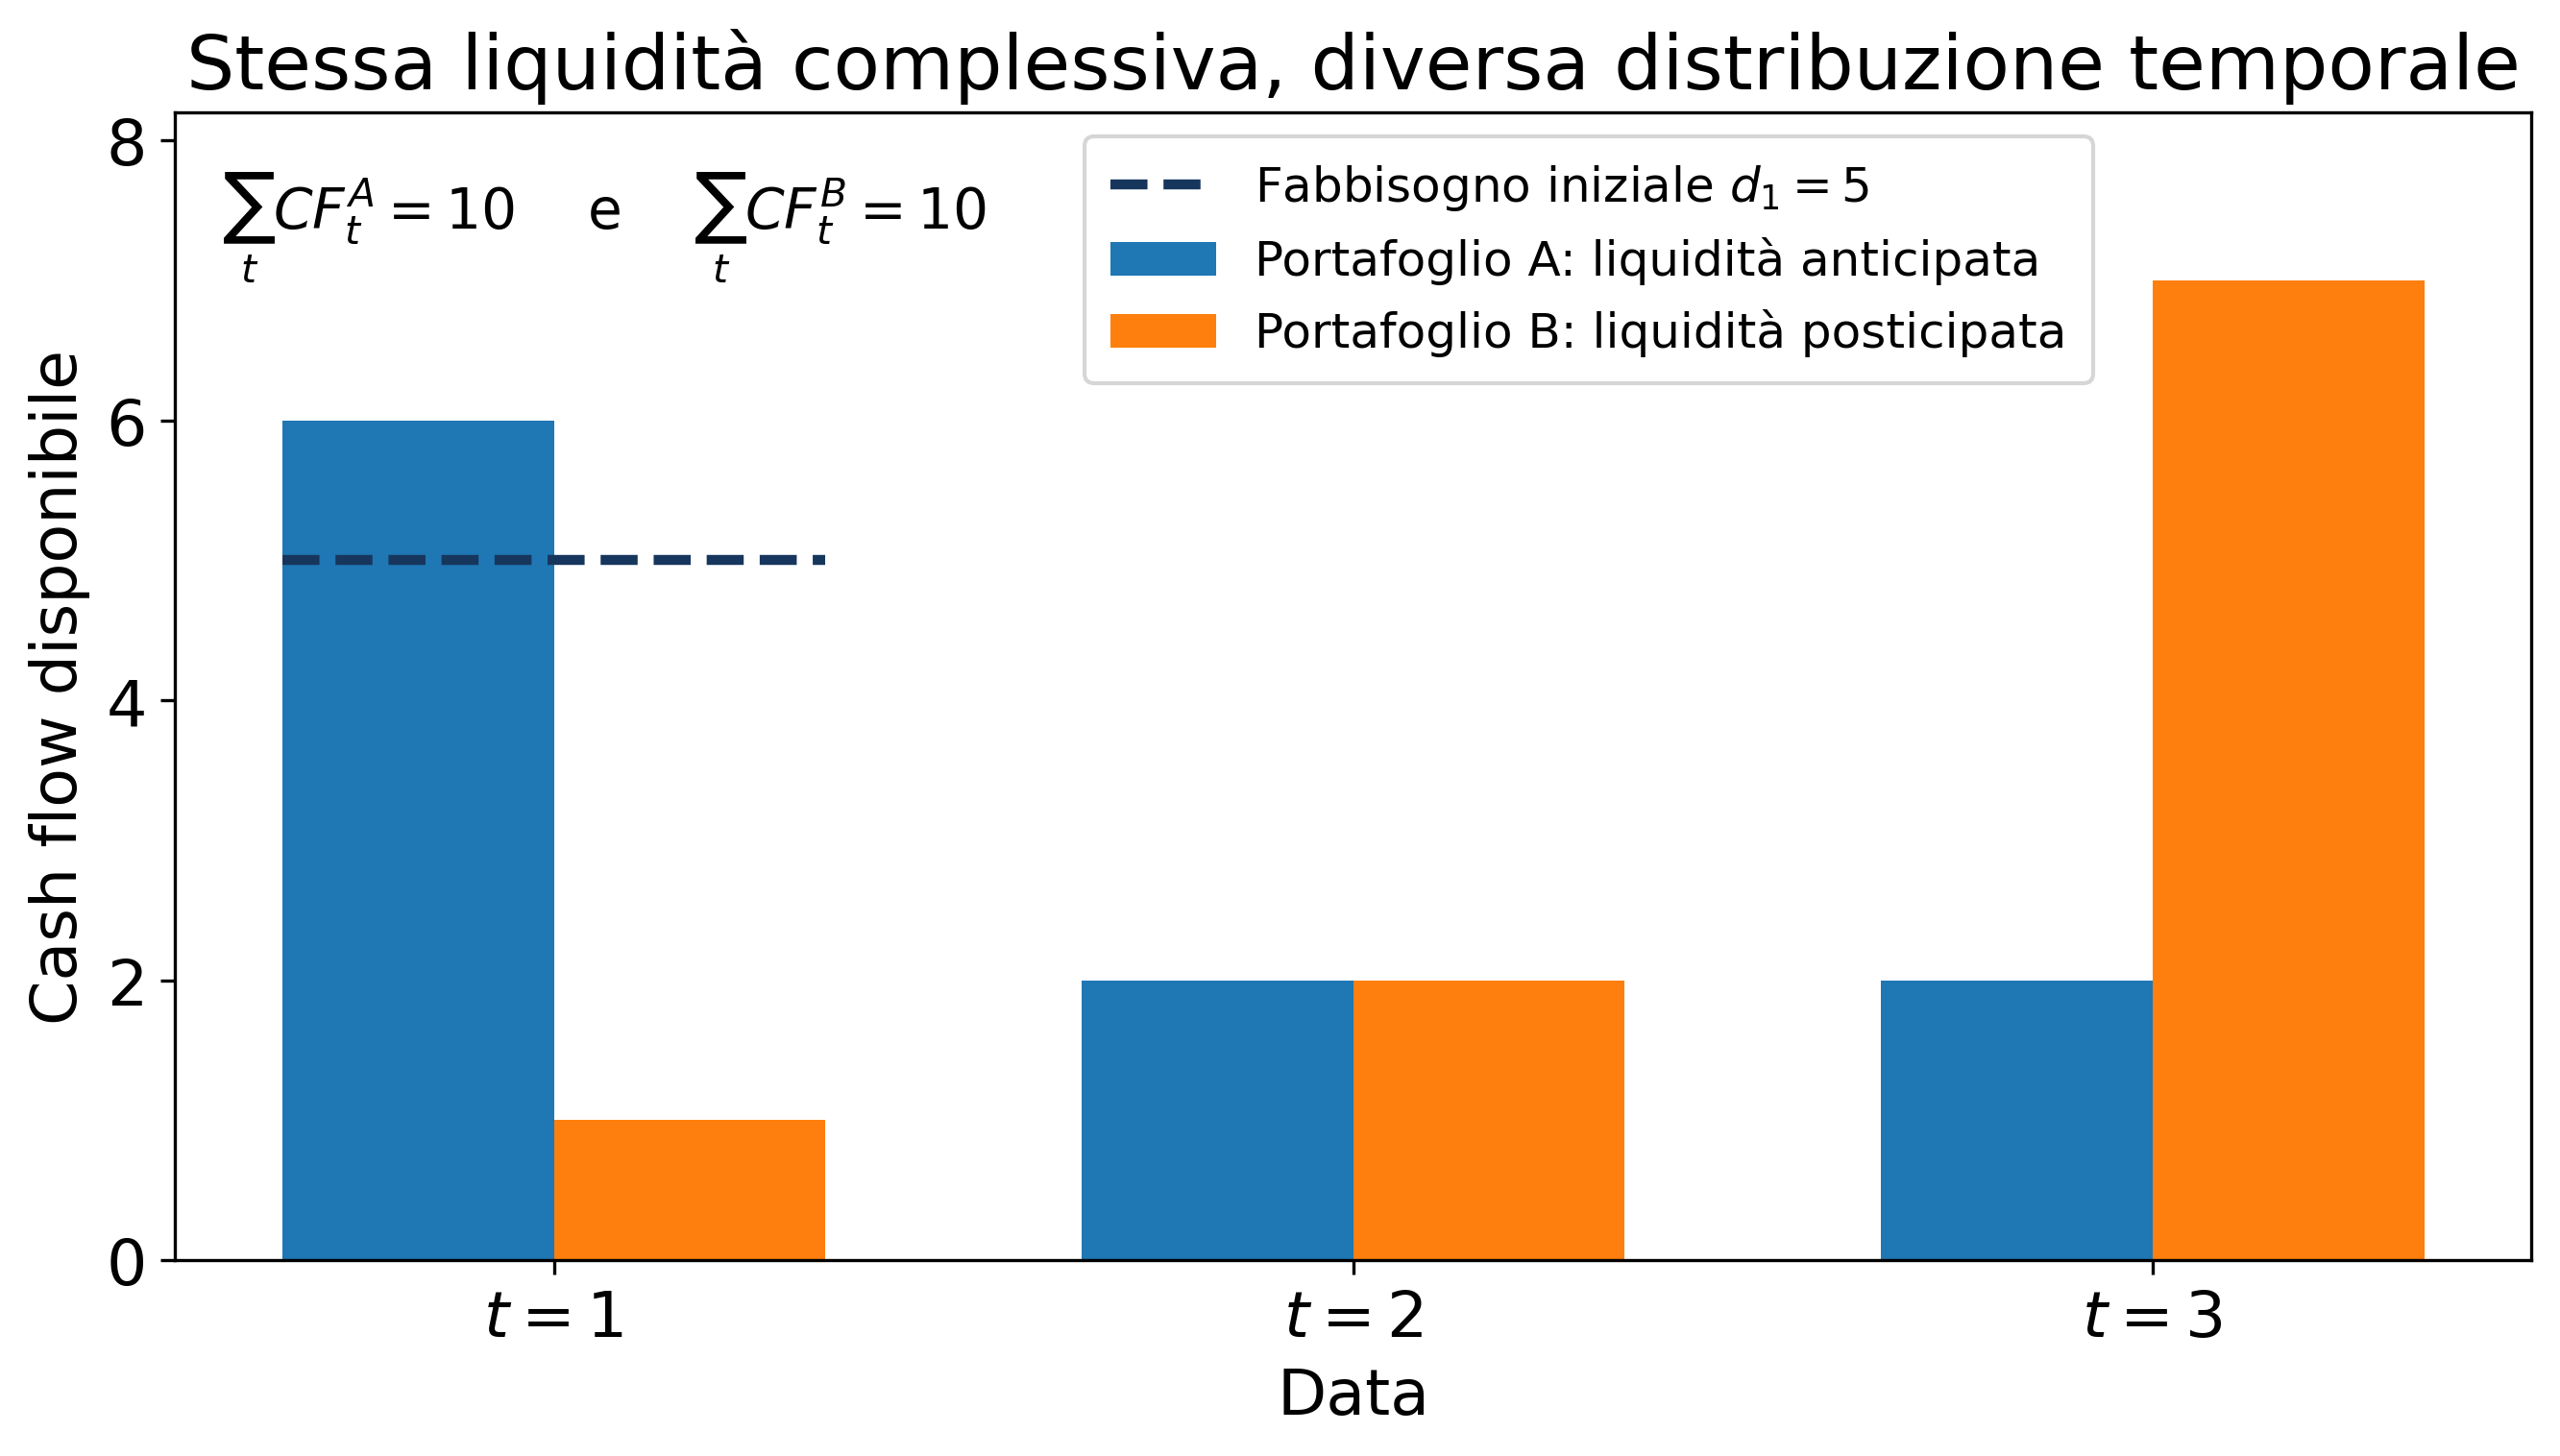
\includegraphics[width=0.90\textwidth]
{../graphics/Cap12_liquidita_aggregata_temporale.png}
\caption{Due portafogli con lo stesso cash flow complessivo ma con diversa
distribuzione temporale. Il portafoglio $A$ produce liquidit\`a in misura
sufficiente a soddisfare il fabbisogno $d_1=5$ alla prima data; il
portafoglio $B$ concentra invece gran parte dei propri flussi alla data
finale.}
\label{fig:cap12-liquidita-aggregata-temporale}
\end{figure}

La Figura~\ref{fig:cap12-liquidita-aggregata-temporale} mostra quindi che la
somma dei cash flow lungo l'intero orizzonte non \`e sufficiente per valutare
la capacit\`a della banca di far fronte ai propri impegni.

La differenza rilevante non riguarda soltanto la quantit\`a complessiva di
liquidit\`a, ma la sua distribuzione nel tempo:

\[
\text{quanto}
\qquad\longrightarrow\qquad
\text{quanto e quando}.
\]

Lo stesso problema si presenta dal lato delle passivit\`a. Una banca non deve
soddisfare un unico fabbisogno aggregato, ma una successione di obblighi,
rimborsi e deflussi collocati in date differenti. La compatibilit\`a tra
attivo e passivo richiede pertanto di confrontare, periodo per periodo, i
flussi prodotti dalle attivit\`a con le risorse richieste dalle passivit\`a.

Introduciamo quindi una sequenza di date

\[
t=0,1,\ldots,T.
\]

Il tempo $t=0$ rappresenta la data nella quale viene scelta la composizione
iniziale del bilancio; le date $t=1,\ldots,T$ rappresentano invece le
scadenze future nelle quali si manifestano cash flow e fabbisogni.

Il problema non consiste pi\`u soltanto nello scegliere una composizione
dell'attivo che soddisfi un requisito complessivo di liquidit\`a. Occorre
scegliere una struttura del bilancio che renda compatibili i flussi generati
dall'attivo con i fabbisogni del passivo lungo l'intero orizzonte temporale.

Il passaggio centrale pu\`o essere sintetizzato come

\[
\boxed{
\text{requisito aggregato di liquidit\`a}
\quad\longrightarrow\quad
\text{bilanci di liquidit\`a alle diverse date}.
}
\]

Questa estensione costituisce il punto di ingresso
nell'Asset--Liability Management deterministico. Il problema resta un
programma lineare: non viene introdotta una nuova classe di ottimizzazione.
Cambiano invece la struttura dei dati e dei vincoli, perch\'e le decisioni
devono ora essere coerenti con una successione di cash flow e fabbisogni
distribuiti nel tempo.

\section{Cash flow degli attivi e fabbisogni alle diverse date}

\label{sec:cap12-cash-flow-fabbisogni}

La sezione precedente ha mostrato che due portafogli con lo stesso cash flow
complessivo possono avere capacit\`a molto diverse di fronteggiare i
fabbisogni della banca. Per rappresentare questa differenza occorre descrivere
separatamente i flussi monetari prodotti alle diverse date.

Consideriamo l'orizzonte discreto

\[
t=0,1,\ldots,T,
\]

e manteniamo il vettore delle decisioni iniziali

\[
x=
\begin{pmatrix}
x_1\\
\vdots\\
x_n
\end{pmatrix},
\]

dove $x_j$ rappresenta l'ammontare destinato alla classe di attivo $j$ al
tempo $0$.

\subsection{Il profilo temporale dei cash flow}

Per ogni attivit\`a $j$ e per ogni data futura $t$, indichiamo con

\[
a_{tj}
\]

il cash flow monetario disponibile alla data $t$ per una unit\`a investita
nell'attivit\`a $j$ al tempo $0$.

L'investimento $x_j$ produce quindi alla data $t$ il flusso

\[
a_{tj}x_j.
\]

Per effetto dell'ipotesi di proporzionalit\`a gi\`a introdotta nel
Capitolo 11, il coefficiente $a_{tj}$ viene trattato come indipendente
dall'ammontare investito. Il cash flow complessivamente prodotto dall'attivo
alla data $t$ \`e pertanto

\[
\sum_{j=1}^{n}a_{tj}x_j.
\]

I coefficienti possono essere raccolti nella matrice dei cash flow

\[
A^{\mathrm{CF}}
=
\begin{pmatrix}
a_{11} & a_{12} & \cdots & a_{1n}\\
a_{21} & a_{22} & \cdots & a_{2n}\\
\vdots & \vdots & \ddots & \vdots\\
a_{T1} & a_{T2} & \cdots & a_{Tn}
\end{pmatrix}.
\]

La matrice $A^{\mathrm{CF}}$ ha $T$ righe e $n$ colonne.

Ogni colonna

\[
\begin{pmatrix}
a_{1j}\\
a_{2j}\\
\vdots\\
a_{Tj}
\end{pmatrix}
\]

descrive il profilo temporale dei cash flow prodotti da una unit\`a della
classe di attivo $j$.

Ogni riga

\[
(a_{t1},\ldots,a_{tn})
\]

descrive invece i cash flow unitari prodotti alla data $t$ dalle diverse
classi di attivo.

Questa organizzazione mantiene la logica matriciale introdotta nel
Capitolo 11. Una colonna continua a descrivere come una variabile decisionale
contribuisce ai diversi requisiti del modello; nel problema multiperiodale,
tali contributi sono ora distinti anche in base alla data nella quale si
manifestano.

\subsection{Il profilo dei fabbisogni}

Dal lato delle passivit\`a, indichiamo con

\[
d_t\geq0
\]

il fabbisogno monetario che deve essere soddisfatto alla data $t$.

La quantit\`a $d_t$ rappresenta l'ammontare di risorse che la banca deve
rendere disponibile in quella data. A seconda della specificazione del
modello, esso pu\`o comprendere rimborsi di passivit\`a, pagamenti
contrattuali, deflussi della raccolta o altri impieghi di liquidit\`a.

Nel modello deterministico sviluppato in questo capitolo, i valori

\[
d_1,d_2,\ldots,d_T
\]

sono trattati come dati noti prima della soluzione del problema e vengono
raccolti nel vettore

\[
d=
\begin{pmatrix}
d_1\\
d_2\\
\vdots\\
d_T
\end{pmatrix}.
\]

La natura deterministica di $d_t$ non implica che i futuri deflussi siano
certi nella realt\`a. Significa che il modello analizza le conseguenze di uno
specifico profilo di fabbisogni assunto come dato nella formulazione
considerata.

Pi\`u avanti il modo in cui tali fabbisogni vengono determinati sar\`a
collegato in modo esplicito alle condizioni economico-finanziarie e alla
situazione patrimoniale della banca. Per il momento, tuttavia, interessa
isolare il problema fondamentale del coordinamento temporale tra risorse
disponibili e risorse richieste.

\begin{figure}[htbp]
\centering
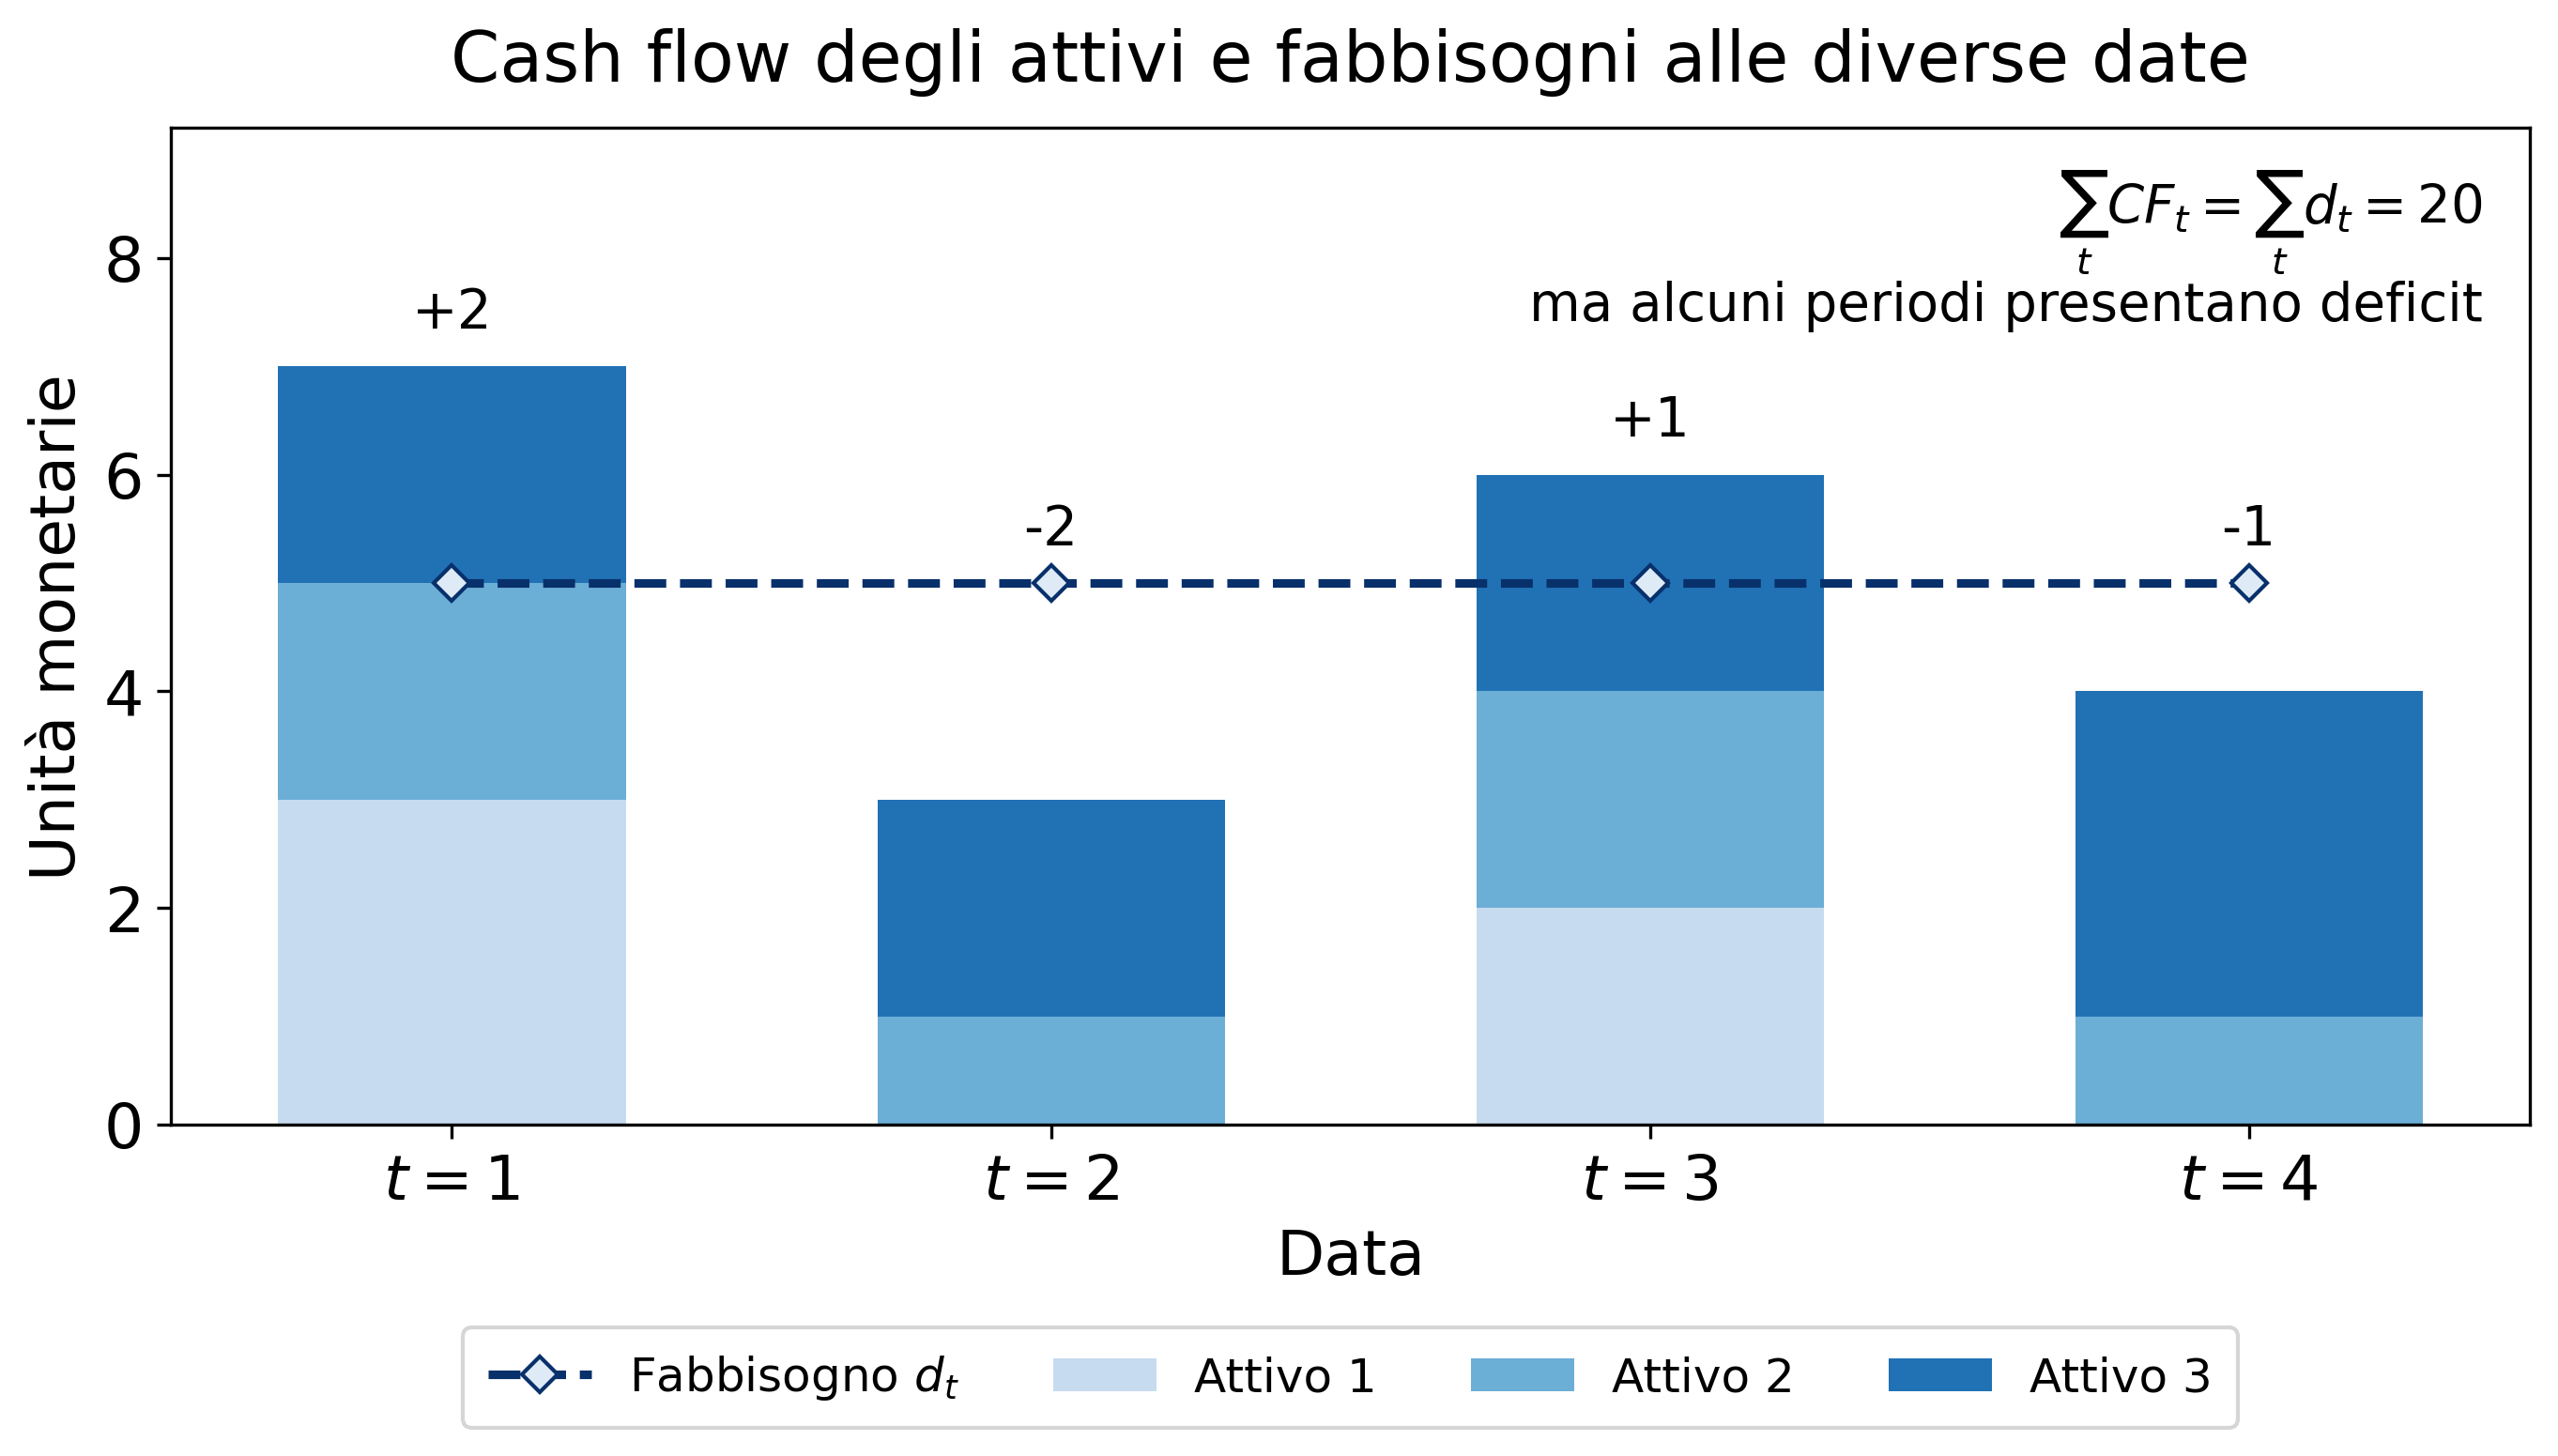
\includegraphics[width=0.92\textwidth]
{../graphics/Cap12_cashflow_attivi_fabbisogni.png}
\caption{Cash flow prodotti dalle diverse classi di attivo e fabbisogni
alle quattro date. Pur coincidendo i cash flow complessivi e i fabbisogni
complessivi sull'intero orizzonte, il profilo temporale presenta surplus
alle date $t=1$ e $t=3$ e deficit alle date $t=2$ e $t=4$.}
\label{fig:cap12-cashflow-fabbisogni}
\end{figure}

La Figura~\ref{fig:cap12-cashflow-fabbisogni} mostra perch\'e il confronto
aggregato non \`e sufficiente. Sull'intero orizzonte le risorse prodotte
dagli attivi coincidono con i fabbisogni:

\[
\sum_{t=1}^{T}CF_t
=
\sum_{t=1}^{T}d_t.
\]

Ci\`o non impedisce tuttavia la presenza di deficit in singole date.
L'Asset--Liability Management deve quindi verificare non soltanto
l'equilibrio complessivo delle risorse, ma la loro disponibilit\`a nel
momento in cui i pagamenti devono essere effettuati.

\subsection{Una prima formulazione: cash-flow matching per data}

Una prima formulazione consiste nel richiedere che, a ciascuna data, i cash
flow prodotti dagli attivi siano almeno sufficienti a coprire il fabbisogno
corrispondente:

\[
\sum_{j=1}^{n}a_{tj}x_j
\geq
d_t,
\qquad
t=1,\ldots,T.
\]

In forma matriciale,

\[
A^{\mathrm{CF}}x
\geq
d.
\]

Il singolo requisito aggregato di liquidit\`a del Capitolo 11 viene quindi
sostituito da $T$ requisiti distinti. La dimensione temporale non viene pi\`u
compressa in un unico coefficiente: per ciascuna data il modello confronta le
risorse monetarie prodotte dall'attivo con il corrispondente fabbisogno.

Questa formulazione rappresenta un primo modello di \emph{cash-flow
matching}. Una composizione dell'attivo \`e ammissibile soltanto se i cash
flow disponibili risultano sufficienti in tutte le date considerate.

Il passaggio dal requisito aggregato

\[
\sum_{j=1}^{n}q_jx_j
\geq
Q_{\min}
\]

ai vincoli

\[
\sum_{j=1}^{n}a_{tj}x_j
\geq
d_t,
\qquad
t=1,\ldots,T,
\]

rende esplicita una differenza fondamentale. Nel primo caso la liquidit\`a
viene misurata come caratteristica complessiva della composizione
dell'attivo; nel secondo viene confrontata con fabbisogni che possiedono una
scadenza precisa.

\subsection{Il limite del matching separato per data}

La formulazione precedente introduce correttamente il tempo, ma considera
ancora ogni data come se fosse indipendente dalle altre.

Supponiamo che, alla data $t$, il portafoglio produca un cash flow superiore
al fabbisogno:

\[
\sum_{j=1}^{n}a_{tj}x_j
>
d_t.
\]

La differenza

\[
\sum_{j=1}^{n}a_{tj}x_j-d_t
\]

rappresenta una disponibilit\`a monetaria residua dopo avere soddisfatto il
fabbisogno della data $t$.

Nei vincoli di cash-flow matching appena formulati, tuttavia, questa
eccedenza non compare nel periodo successivo. Le risorse disponibili alla
data $t$ che non vengono utilizzate scompaiono dal modello e non possono
contribuire alla copertura del fabbisogno alla data $t+1$.

Si tratta di una limitazione economicamente rilevante. Una banca pu\`o
conservare una parte della liquidit\`a disponibile oppure reinvestirla in una
forma compatibile con l'orizzonte successivo. La posizione di liquidit\`a di
una data dipende quindi anche da quanto \`e accaduto nelle date precedenti.

Il problema ALM non pu\`o essere descritto come una semplice successione di
$T$ vincoli indipendenti. Occorre introdurre una variabile che rappresenti la
liquidit\`a residua trasferita da un periodo al successivo.

Il passaggio successivo \`e quindi

\[
\boxed{
\text{cash-flow matching per data}
\quad\longrightarrow\quad
\text{bilanci di liquidit\`a collegati nel tempo}.
}
\]

L'introduzione di questa variabile render\`a esplicita la dipendenza tra il
vincolo relativo alla data $t$ e quello relativo alla data $t+1$ e
costituir\`a il primo vero elemento intertemporale del modello ALM.

\section{Liquidit\`a residua e bilanci intertemporali}

\label{sec:cap12-bilanci-intertemporali}

Il cash-flow matching introdotto nella
Sezione~\ref{sec:cap12-cash-flow-fabbisogni} confronta, per ogni data,
i flussi prodotti dall'attivo con il corrispondente fabbisogno:

\[
\sum_{j=1}^{n}a_{tj}x_j
\geq
d_t,
\qquad
t=1,\ldots,T.
\]

Questa formulazione riconosce che la liquidit\`a deve essere disponibile
nella data in cui viene richiesta, ma non descrive ancora che cosa accade
quando i cash flow prodotti in un periodo superano il fabbisogno dello stesso
periodo.

In una gestione intertemporale, l'eccedenza non scompare. Pu\`o essere
conservata e utilizzata nelle date successive. Per rappresentare questo
meccanismo introduciamo una nuova variabile decisionale.

\begin{definition}[Giacenza di liquidit\`a]

Per ogni data $t=1,\ldots,T$, indichiamo con

\[
g_t\geq0
\]

la liquidit\`a che rimane disponibile immediatamente dopo avere soddisfatto
il fabbisogno $d_t$.

\end{definition}

La variabile $g_t$ \`e quindi uno \emph{stock}, misurato in unit\`a
monetarie. Non rappresenta un nuovo cash flow prodotto dall'attivo, ma la
parte delle risorse disponibili alla data $t$ che non viene utilizzata e
viene trasferita al periodo successivo.

\subsection{Il primo bilancio temporale}

Consideriamo inizialmente la prima data, $t=1$.

I cash flow prodotti dall'attivo sono

\[
\sum_{j=1}^{n}a_{1j}x_j.
\]

Queste risorse devono essere utilizzate per soddisfare il fabbisogno $d_1$;
l'eventuale eccedenza costituisce la giacenza $g_1$.

Il bilancio monetario alla prima data \`e quindi

\[
\sum_{j=1}^{n}a_{1j}x_j
=
d_1+g_1.
\]

La relazione \`e un'uguaglianza, non una disuguaglianza. Tutte le risorse
monetarie disponibili alla data $1$ devono avere una destinazione: una parte
viene utilizzata per soddisfare il fabbisogno, la parte restante viene
conservata come liquidit\`a.

Equivalentemente,

\[
g_1
=
\sum_{j=1}^{n}a_{1j}x_j-d_1.
\]

La condizione

\[
g_1\geq0
\]

garantisce che il fabbisogno della prima data possa essere interamente
soddisfatto.

\subsection{Il collegamento con la data successiva}

Alla data $t=2$ la banca dispone di due fonti di liquidit\`a:

\begin{itemize}

\item i nuovi cash flow prodotti dagli attivi,

\[
\sum_{j=1}^{n}a_{2j}x_j;
\]

\item la giacenza $g_1$ trasferita dalla data precedente.

\end{itemize}

Se, in una prima formulazione, assumiamo che la liquidit\`a trasferita non
produca rendimento, il bilancio alla seconda data diventa

\[
\sum_{j=1}^{n}a_{2j}x_j
+
g_1
=
d_2+g_2.
\]

Pi\`u in generale, per

\[
t=2,\ldots,T,
\]

si ottiene

\[
\sum_{j=1}^{n}a_{tj}x_j
+
g_{t-1}
=
d_t+g_t.
\]

Il sistema completo dei bilanci temporali \`e pertanto

\[
\begin{array}{rcl}
\displaystyle
\sum_{j=1}^{n}a_{1j}x_j
-
g_1
&=&
d_1,
\\[8pt]
\displaystyle
\sum_{j=1}^{n}a_{2j}x_j
+
g_1-g_2
&=&
d_2,
\\
&\vdots&
\\
\displaystyle
\sum_{j=1}^{n}a_{Tj}x_j
+
g_{T-1}-g_T
&=&
d_T.
\end{array}
\]

La differenza rispetto al cash-flow matching separato per data \`e
fondamentale. La variabile $g_t$ compare contemporaneamente nel bilancio
della data $t$ e in quello della data $t+1$.

Il vincolo relativo a una data non pu\`o quindi pi\`u essere interpretato
isolatamente:

\[
\boxed{
g_t
\text{ collega il bilancio della data }t
\text{ al bilancio della data }t+1.
}
\]

Questa \`e la struttura intertemporale essenziale del modello.

\subsection{La liquidit\`a come variabile di stato}

La giacenza $g_t$ possiede una funzione diversa dalle variabili iniziali
$x_j$.

Le quantit\`a

\[
x_1,\ldots,x_n
\]

determinano la composizione dell'attivo \textbf{scelta} al tempo $0$.

La quantit\`a

\[
g_t
\]

descrive invece la posizione di liquidit\`a con la quale la banca conclude la
data $t$ e affronta la data successiva.

In questo senso, $g_t$ pu\`o essere interpretata come una semplice
\emph{variabile di stato}: sintetizza una conseguenza delle decisioni e dei
cash flow passati che diventa rilevante per i vincoli futuri.

Dal bilancio temporale segue infatti la relazione ricorsiva

\[
g_t
=
g_{t-1}
+
\sum_{j=1}^{n}a_{tj}x_j
-
d_t,
\qquad
t=1,\ldots,T,
\]

ponendo per il momento

\[
g_0=0.
\]

La liquidit\`a disponibile alla fine di ogni data dipende quindi dalla
liquidit\`a ereditata dal periodo precedente, dai nuovi flussi prodotti
dall'attivo e dal fabbisogno corrente.

Questa rappresentazione rende esplicito un principio centrale
dell'Asset--Liability Management:

\[
\boxed{
\begin{array}{c}
\text{la posizione finanziaria a una data dipende anche}\\
\text{dalle decisioni e dai saldi accumulati nelle date precedenti}
\end{array}
}
\]

\subsection{Il rendimento della liquidit\`a trasferita}

L'ipotesi secondo cui la liquidit\`a trasferita da una data alla successiva
mantenga invariato il proprio valore \`e utile per isolare la struttura dei
bilanci, ma pu\`o essere raffinata.

Supponiamo che la giacenza disponibile dopo la data $t-1$ possa essere
impiegata fino alla data $t$ a un tasso deterministico $r_{t-1}$.

Una unit\`a monetaria detenuta alla fine della data $t-1$ diventa quindi

\[
1+r_{t-1}
\]

unit\`a alla data $t$.

Per $t=2,\ldots,T$, il bilancio diventa

\[
\sum_{j=1}^{n}a_{tj}x_j
+
(1+r_{t-1})g_{t-1}
=
d_t+g_t.
\]

Per la prima data resta

\[
\sum_{j=1}^{n}a_{1j}x_j
=
d_1+g_1,
\]

se si assume che non esista una giacenza iniziale separata dalla composizione
$x$ scelta al tempo $0$.

Il sistema pu\`o quindi essere scritto come

\[
\begin{array}{rcl}
\displaystyle
\sum_{j=1}^{n}a_{1j}x_j-g_1
&=&
d_1,
\\[8pt]
\displaystyle
\sum_{j=1}^{n}a_{2j}x_j
+
(1+r_1)g_1-g_2
&=&
d_2,
\\
&\vdots&
\\
\displaystyle
\sum_{j=1}^{n}a_{Tj}x_j
+
(1+r_{T-1})g_{T-1}-g_T
&=&
d_T.
\end{array}
\]

Il coefficiente $1+r_{t-1}$ non modifica la natura lineare del modello,
poich\'e il tasso $r_{t-1}$ \`e trattato come un dato deterministico.

\subsection{Condizione finale}

La variabile $g_T$ rappresenta la liquidit\`a residua alla fine
dell'orizzonte considerato. Il suo trattamento dipende dalla funzione del
modello.

Se l'orizzonte termina quando tutti gli obblighi rilevanti sono stati
soddisfatti e non si attribuisce valore alla liquidit\`a residua, pu\`o essere
imposta la condizione

\[
g_T=0.
\]

Se invece la liquidit\`a finale rappresenta una risorsa economicamente utile
oltre l'orizzonte del modello, essa non deve essere forzata a zero: dovr\`a
essere mantenuta come variabile oppure valorizzata nella funzione obiettivo.

La condizione terminale non \`e quindi un dettaglio tecnico. Stabilisce che
cosa il modello considera economicamente rilevante al termine
dell'orizzonte.

\subsection{Dal matching al bilancio dinamico}

Il passaggio compiuto in questa sezione pu\`o essere riassunto confrontando le
due formulazioni.

Nel cash-flow matching separato per data:

\[
\sum_{j=1}^{n}a_{tj}x_j
\geq
d_t.
\]

Nel modello con trasferimento della liquidit\`a:

\[
\sum_{j=1}^{n}a_{tj}x_j
+
(1+r_{t-1})g_{t-1}
=
d_t+g_t.
\]

Nel primo caso ciascuna data costituisce un confronto autonomo tra flussi e
fabbisogni. Nel secondo, il saldo di un periodo diventa una risorsa del
periodo successivo.

La programmazione rimane lineare, ma la struttura economica del problema
cambia profondamente: il modello non confronta pi\`u soltanto attivit\`a e
passivit\`a alle singole date, bens\`i descrive l'evoluzione nel tempo della
posizione di liquidit\`a della banca.

Questo collegamento prepara il passo successivo. La liquidit\`a accumulata
internamente non \`e infatti l'unico strumento con cui una banca pu\`o
fronteggiare un fabbisogno temporaneo. Quando i cash flow dell'attivo e la
giacenza disponibile non sono sufficienti, la banca pu\`o ricorrere a
funding esterno. Tale scelta produce liquidit\`a nella data corrente, ma
genera contemporaneamente un obbligo di rimborso futuro.

\section{Funding esterno e obblighi di rimborso}

\label{sec:cap12-funding}

I bilanci intertemporali introdotti nella
Sezione~\ref{sec:cap12-bilanci-intertemporali} assumono che la banca possa
soddisfare i propri fabbisogni utilizzando esclusivamente i cash flow prodotti
dall'attivo e la liquidit\`a accumulata nelle date precedenti.

Questa rappresentazione mette in evidenza il collegamento temporale tra le
diverse date, ma trascura una possibilit\`a importante. Se le risorse interne
non sono sufficienti a soddisfare un fabbisogno corrente, la banca pu\`o
ricorrere a una fonte esterna di funding.

Il funding modifica la disponibilit\`a di liquidit\`a nella data in cui viene
raccolto, ma non costituisce una risorsa gratuita. Le somme ottenute devono
essere rimborsate in una data successiva insieme al relativo costo
finanziario.

\subsection{Una fonte di funding a un periodo}

Per mantenere leggibile la struttura del modello, consideriamo una sola forma
stilizzata di funding con durata pari a un periodo.

Per

\[
t=1,\ldots,T-1,
\]

indichiamo con

\[
u_t\geq0
\]

l'ammontare di funding raccolto alla data $t$.

La quantit\`a $u_t$ \`e immediatamente disponibile e pu\`o quindi essere
utilizzata per soddisfare il fabbisogno della stessa data.

Supponiamo che il funding raccolto alla data $t$ debba essere rimborsato alla
data $t+1$ a un tasso deterministico $\rho_t$. L'obbligo di rimborso generato
da $u_t$ \`e pertanto

\[
(1+\rho_t)u_t.
\]

La sequenza economica \`e quindi

\[
\boxed{
\begin{array}{c}
\text{funding raccolto alla data }t:\quad u_t\\[3pt]
\downarrow\\[3pt]
\text{liquidit\`a disponibile alla data }t\\[3pt]
\downarrow\\[3pt]
\text{rimborso alla data }t+1:\quad (1+\rho_t)u_t
\end{array}
}
\]

Il funding trasferisce quindi risorse dalla data futura alla data corrente:
aumenta la liquidit\`a disponibile oggi, ma riduce quella disponibile domani.

\subsection{Il bilancio alla prima data}

Alla data $t=1$ la banca dispone dei cash flow prodotti dagli attivi,

\[
\sum_{j=1}^{n}a_{1j}x_j,
\]

e pu\`o inoltre raccogliere funding per un ammontare $u_1$.

Le risorse vengono utilizzate per soddisfare il fabbisogno $d_1$ e
l'eventuale eccedenza viene mantenuta come giacenza $g_1$.

Il bilancio diventa quindi

\[
\sum_{j=1}^{n}a_{1j}x_j
+
u_1
=
d_1+g_1.
\]

Rispetto alla formulazione della sezione precedente, il termine $u_1$
costituisce una nuova fonte di liquidit\`a.

Il suo utilizzo produce tuttavia un effetto sul periodo successivo.

\subsection{Il bilancio nelle date intermedie}

Consideriamo una generica data

\[
t=2,\ldots,T-1.
\]

Le risorse disponibili sono ora costituite da tre componenti:

\begin{itemize}

\item i cash flow prodotti dagli attivi,

\[
\sum_{j=1}^{n}a_{tj}x_j;
\]

\item la giacenza proveniente dalla data precedente, capitalizzata al tasso
$r_{t-1}$,

\[
(1+r_{t-1})g_{t-1};
\]

\item il nuovo funding raccolto alla data corrente,

\[
u_t.
\]

\end{itemize}

A queste risorse si contrappongono tre utilizzi:

\begin{itemize}

\item il fabbisogno corrente $d_t$;

\item il rimborso del funding raccolto alla data precedente,

\[
(1+\rho_{t-1})u_{t-1};
\]

\item la nuova giacenza di liquidit\`a $g_t$.

\end{itemize}

Il bilancio intertemporale completo \`e quindi

\[
\sum_{j=1}^{n}a_{tj}x_j
+
(1+r_{t-1})g_{t-1}
+
u_t
=
d_t
+
(1+\rho_{t-1})u_{t-1}
+
g_t.
\]

La stessa variabile $u_t$ svolge quindi due ruoli in date consecutive:

\[
u_t
\]

\`e una risorsa nel bilancio della data $t$, mentre

\[
(1+\rho_t)u_t
\]

diventa un utilizzo nel bilancio della data $t+1$.

Il funding introduce cos\`i un secondo collegamento intertemporale, accanto a
quello gi\`a prodotto dalla giacenza $g_t$.

\begin{figure}[htbp]
\centering
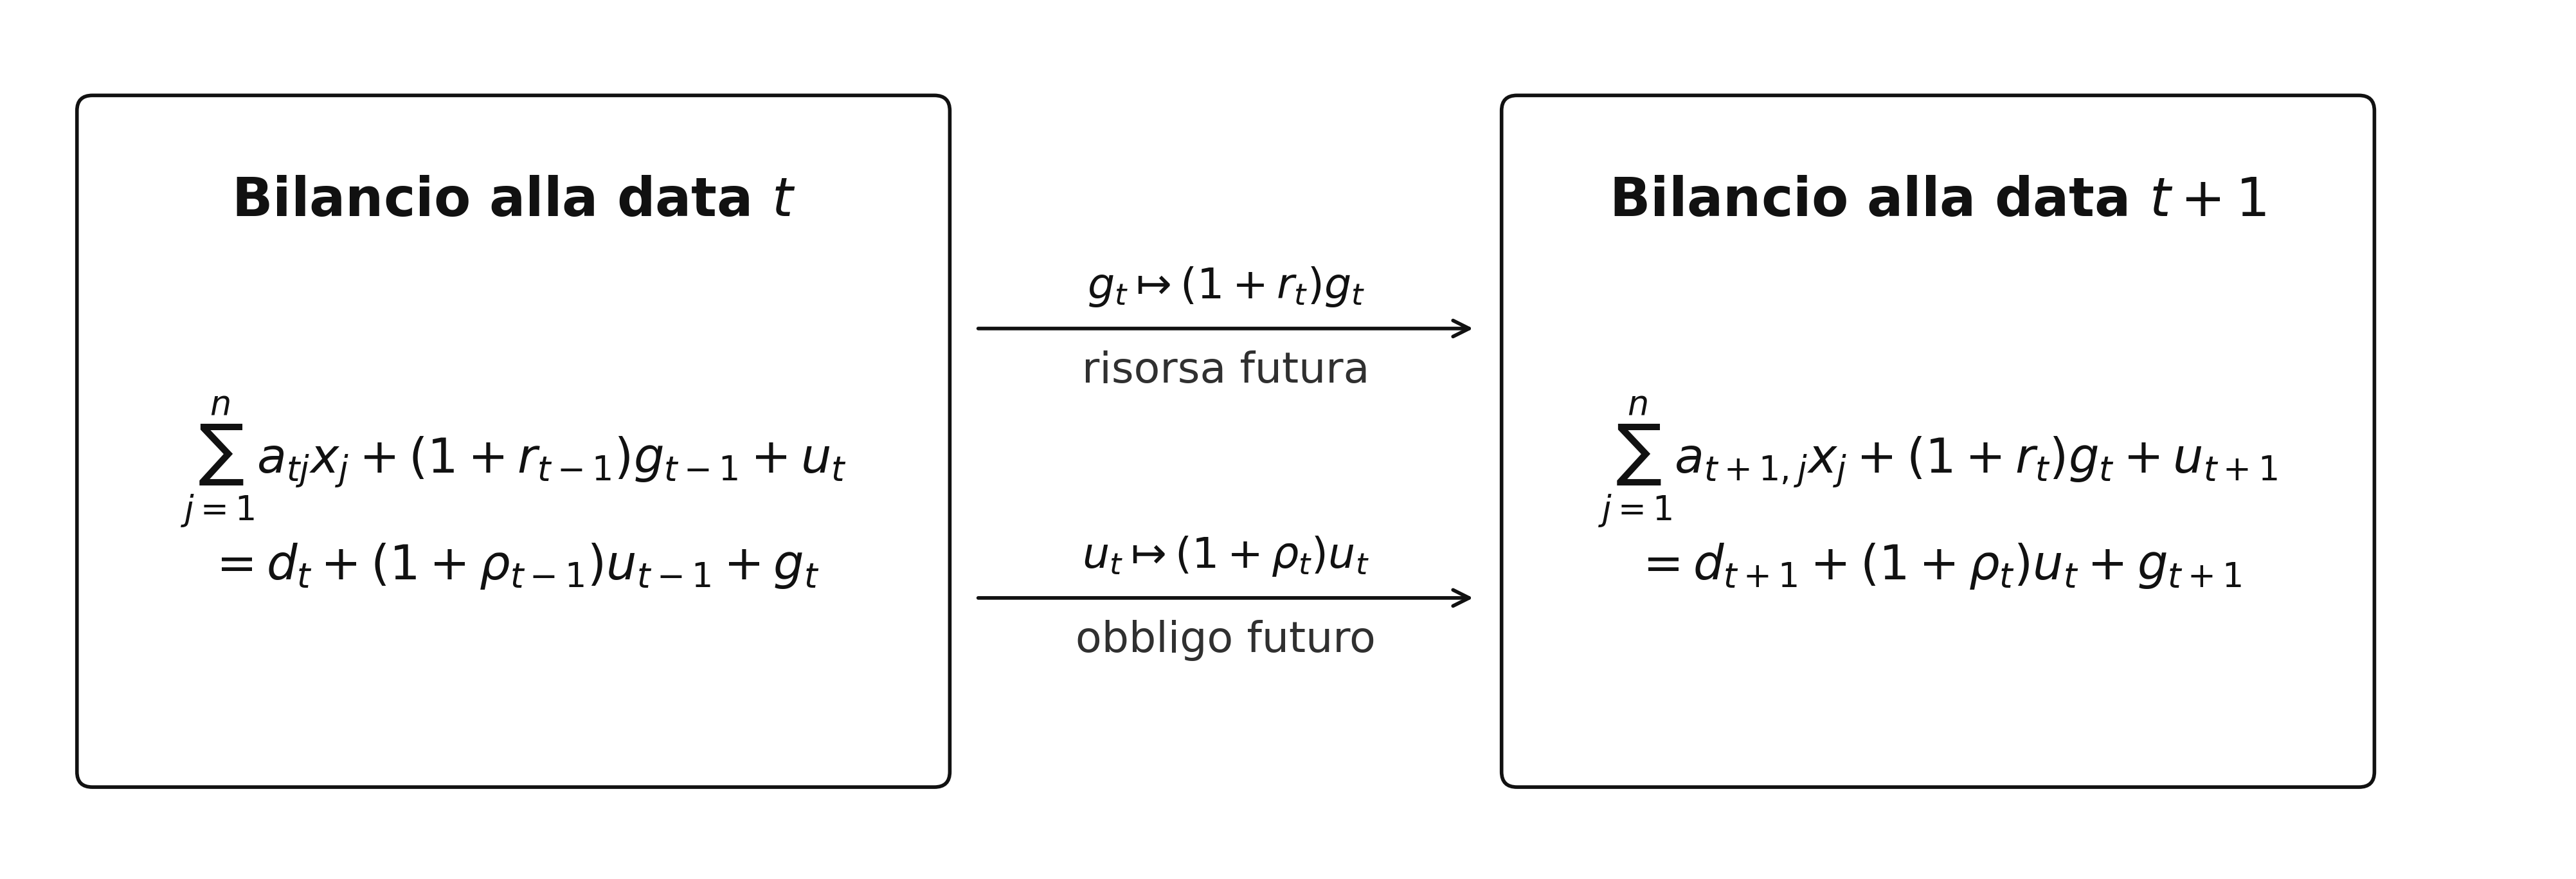
\includegraphics[width=0.96\textwidth]
{../graphics/Cap12_bilancio_intertemporale.png}
\caption{Collegamento tra due bilanci di liquidit\`a consecutivi. La
giacenza $g_t$ costituisce una risorsa disponibile alla data successiva,
mentre il funding $u_t$ raccolto alla data corrente genera un obbligo di
rimborso pari a $(1+\rho_t)u_t$ alla data successiva.}
\label{fig:cap12-bilancio-intertemporale}
\end{figure}

La Figura~\ref{fig:cap12-bilancio-intertemporale} rende visibili i due
collegamenti fondamentali tra date consecutive. La giacenza trasferisce
risorse verso il futuro; il funding trasferisce invece risorse dal futuro
al presente e genera per questo un successivo obbligo di rimborso.

Le due variabili hanno quindi effetti temporali opposti:

\[
g_t
\quad\text{accumula una risorsa per il periodo successivo},
\]

mentre

\[
u_t
\quad\text{anticipa una risorsa creando un'obbligazione futura}.
\]

La struttura intertemporale del modello nasce precisamente dalla presenza
simultanea di questi collegamenti.

\subsection{Il bilancio alla data finale}

Alla data finale $T$ non introduciamo nuovo funding. Questa scelta garantisce
che ogni posizione di funding aperta all'interno dell'orizzonte venga anche
rimborsata entro l'orizzonte stesso.

Il bilancio finale \`e pertanto

\[
\sum_{j=1}^{n}a_{Tj}x_j
+
(1+r_{T-1})g_{T-1}
=
d_T
+
(1+\rho_{T-1})u_{T-1}
+
g_T.
\]

Il sistema completo pu\`o quindi essere scritto come

\[
\begin{array}{rcl}
\displaystyle
\sum_{j=1}^{n}a_{1j}x_j+u_1-g_1
&=&
d_1,
\\[8pt]
\displaystyle
\sum_{j=1}^{n}a_{tj}x_j
+
(1+r_{t-1})g_{t-1}
+
u_t
-
(1+\rho_{t-1})u_{t-1}
-
g_t
&=&
d_t,
\\
&&
t=2,\ldots,T-1,
\\[8pt]
\displaystyle
\sum_{j=1}^{n}a_{Tj}x_j
+
(1+r_{T-1})g_{T-1}
-
(1+\rho_{T-1})u_{T-1}
-
g_T
&=&
d_T.
\end{array}
\]

Le condizioni di non negativit\`a sono

\[
g_t\geq0,
\qquad
t=1,\ldots,T,
\]

e

\[
u_t\geq0,
\qquad
t=1,\ldots,T-1.
\]

\subsection{Limiti alla disponibilit\`a di funding}

La possibilit\`a di raccogliere funding non pu\`o essere considerata
illimitata.

Introduciamo pertanto, per ogni data,

\[
\bar{u}_t\geq0,
\]

che rappresenta l'ammontare massimo di funding accessibile alla banca.

Il vincolo

\[
0\leq u_t\leq\bar{u}_t,
\qquad
t=1,\ldots,T-1,
\]

pu\`o riflettere limiti contrattuali, capacit\`a di accesso al mercato,
disponibilit\`a di linee di credito o altri vincoli sulla raccolta
incrementale.

Il parametro $\bar{u}_t$ ha un significato diverso da $u_t$:

\[
u_t
=
\text{decisione di funding},
\]

mentre

\[
\bar{u}_t
=
\text{massima capacit\`a di funding disponibile}.
\]

La banca decide quindi quanto funding utilizzare all'interno di una
capacit\`a data.

\subsection{Costo del funding e assenza di arbitraggio artificiale}

Il tasso $\rho_t$ rappresenta il costo complessivo della fonte di funding
utilizzata tra le date $t$ e $t+1$.

Nello stesso intervallo, la giacenza di liquidit\`a produce il rendimento
$r_t$.

Per evitare che il modello trovi conveniente raccogliere funding unicamente
per investirlo nella giacenza di liquidit\`a, \`e naturale assumere

\[
\rho_t\geq r_t.
\]

In una rappresentazione bancaria realistica ci si attende normalmente

\[
\rho_t>r_t,
\]

poich\'e la raccolta esterna incorpora un costo superiore al rendimento di una
posizione liquida priva di rischio comparabile.

La differenza

\[
\rho_t-r_t
\]

rappresenta quindi, in forma stilizzata, il costo aggiuntivo associato
all'accesso al funding.

Questa condizione non \`e necessaria per la linearit\`a matematica del
problema, ma evita un comportamento economicamente artificiale del modello.

\subsection{Funding e gestione della liquidit\`a}

L'introduzione di $u_t$ modifica il significato del problema ALM.

Senza funding, un'insufficienza dei cash flow e della liquidit\`a accumulata
rende il piano non ammissibile.

Con il funding, la banca dispone di una seconda possibilit\`a:

\[
\text{deficit corrente}
\quad\longrightarrow\quad
\text{funding oggi}
\quad\longrightarrow\quad
\text{obbligo di rimborso domani}.
\]

Il funding non elimina quindi il problema della liquidit\`a. Ne modifica la
distribuzione temporale.

Una scelta di funding che risolve un deficit alla data $t$ pu\`o infatti
rendere pi\`u difficile soddisfare il bilancio alla data $t+1$, a causa del
rimborso

\[
(1+\rho_t)u_t.
\]

La decisione non pu\`o pertanto essere valutata considerando esclusivamente il
periodo corrente.

Il modello comincia cos\`i a rappresentare il nucleo dell'Asset--Liability
Management:

\[
\boxed{
\begin{array}{c}
\text{le risorse disponibili oggi dipendono dalle decisioni passate,}\\
\text{mentre le decisioni assunte oggi modificano i fabbisogni futuri.}
\end{array}
}
\]

La struttura resta interamente lineare. I coefficienti $a_{tj}$, $d_t$,
$r_t$, $\rho_t$ e $\bar{u}_t$ sono, in questa fase, dati deterministici;
$x_j$, $g_t$ e $u_t$ sono invece le variabili attraverso le quali il modello
descrive la composizione dell'attivo e la gestione intertemporale della
liquidit\`a.

La sezione successiva preciser\`a come tali coefficienti possano essere
ricondotti a un ambiente economico-finanziario deterministico e come il
modello ALM possa essere collegato in modo coerente al caso bancario
sviluppato nel Capitolo 11.

\section{L'ambiente economico-finanziario deterministico}

\label{sec:cap12-ambiente-deterministico}

Le sezioni precedenti hanno costruito la struttura intertemporale del modello
ALM. I cash flow degli attivi, la giacenza di liquidit\`a e il funding
collegano le diverse date attraverso i bilanci

\[
\sum_{j=1}^{n}a_{tj}x_j
+
(1+r_{t-1})g_{t-1}
+
u_t
=
d_t
+
(1+\rho_{t-1})u_{t-1}
+
g_t.
\]

Finora i coefficienti

\[
a_{tj},\qquad r_t,\qquad \rho_t,\qquad \bar{u}_t
\]

sono stati trattati semplicemente come dati del modello. In un problema
bancario, tuttavia, tali coefficienti riflettono le condizioni
economico-finanziarie nelle quali la banca opera.

Per rendere esplicito questo collegamento introduciamo, per ogni data
$t=0,1,\ldots,T$, il vettore

\[
\bar{Z}_t
=
\left(
\bar{R}_t,\bar{C}_t,\bar{F}_t
\right).
\]

La barra indica che, nel presente capitolo, l'intera traiettoria

\[
\bar{Z}_0,\bar{Z}_1,\ldots,\bar{Z}_T
\]

\`e considerata nota al momento della formulazione del problema.

Il modello \`e quindi deterministico, ma i valori dei fattori possono variare
nel tempo:

\[
\bar{Z}_t
\neq
\bar{Z}_{t+1}.
\]

La caratteristica deterministica riguarda la conoscenza della traiettoria,
non la sua costanza.

\subsection{Tre dimensioni dell'ambiente finanziario}

Le tre componenti di $\bar{Z}_t$ hanno funzioni economiche distinte.

Il fattore

\[
\bar{R}_t
\]

rappresenta il livello dei tassi privi di rischio rilevante nell'intervallo
considerato. Esso pu\`o essere interpretato come il \emph{prezzo del tempo}:
determina il rendimento delle disponibilit\`a liquide e contribuisce alla
valutazione dei flussi monetari distribuiti nel tempo.

Il fattore

\[
\bar{C}_t
\]

rappresenta il livello dello spread di credito osservato sul mercato. Esso
misura il premio richiesto per detenere esposizioni soggette a rischio di
credito e pu\`o essere interpretato come il \emph{prezzo del rischio di
credito}.

Il fattore

\[
\bar{F}_t
\]

rappresenta invece lo spread o la tensione associata al funding della banca.
Esso misura quanto l'accesso alla raccolta esterna sia costoso o difficile
rispetto a una fonte priva di rischio comparabile e pu\`o essere interpretato
come il \emph{prezzo della scarsit\`a di funding}.

La distinzione pu\`o essere sintetizzata come

\[
\boxed{
\begin{array}{c}
\bar{R}_t:\ \text{prezzo del tempo},\\[3pt]
\bar{C}_t:\ \text{prezzo del rischio di credito},\\[3pt]
\bar{F}_t:\ \text{prezzo della scarsit\`a di funding}.
\end{array}
}
\]

I tre fattori descrivono l'ambiente esterno nel quale la banca opera. Non
dipendono dalle decisioni $x_j$, $g_t$ o $u_t$ assunte nel modello.

\subsection{Dal livello dei tassi al rendimento della liquidit\`a}

Nella Sezione~\ref{sec:cap12-bilanci-intertemporali} il parametro $r_t$
rappresenta il rendimento ottenibile mantenendo una giacenza di liquidit\`a
tra le date $t$ e $t+1$.

Il suo valore pu\`o essere ricondotto al livello del tasso privo di rischio:

\[
r_t
=
r(\bar{R}_t).
\]

Nella rappresentazione pi\`u semplice, se $\bar{R}_t$ indica direttamente il
tasso applicabile alla giacenza nell'intervallo considerato, si pu\`o porre

\[
r_t=\bar{R}_t.
\]

Il bilancio utilizza quindi

\[
(1+\bar{R}_t)g_t
\]

come ammontare disponibile alla data successiva.

La relazione non deve essere interpretata come una legge generale di mercato.
Essa costituisce una specificazione coerente con un modello nel quale la
liquidit\`a residua viene investita per un periodo in una forma a rischio
trascurabile.

\subsection{Il costo del funding}

Il tasso $\rho_t$ introdotto nella
Sezione~\ref{sec:cap12-funding} rappresenta invece il costo del funding
raccolto alla data $t$ e rimborsato alla data $t+1$.

Il suo valore dipende sia dal livello generale dei tassi sia dalle condizioni
specifiche di funding della banca. Una rappresentazione naturale \`e

\[
\rho_t
=
\rho(\bar{R}_t,\bar{F}_t).
\]

Se $\bar{F}_t$ viene misurato direttamente come spread sul tasso privo di
rischio, una specificazione particolarmente semplice \`e

\[
\rho_t
=
\bar{R}_t+\bar{F}_t.
\]

Il rimborso del funding diventa quindi

\[
\left(
1+\bar{R}_t+\bar{F}_t
\right)u_t.
\]

Questa rappresentazione rende esplicita la differenza tra il rendimento della
liquidit\`a e il costo della raccolta esterna. Se

\[
\bar{F}_t>0,
\]

allora

\[
\rho_t>r_t,
\]

coerentemente con l'ipotesi introdotta nella sezione precedente.

Il funding \`e quindi tanto pi\`u costoso quanto maggiore \`e la tensione
associata alla raccolta della banca.

\subsection{Disponibilit\`a di funding}

Le condizioni di funding possono incidere non soltanto sul costo della
raccolta, ma anche sull'ammontare massimo accessibile.

Il parametro

\[
\bar{u}_t
\]

rappresenta la capacit\`a massima di funding disponibile alla data $t$.

In forma generale si pu\`o scrivere

\[
\bar{u}_t
=
\bar{u}(\bar{F}_t).
\]

In condizioni di funding favorevoli la banca pu\`o disporre di una maggiore
capacit\`a di raccolta; in condizioni di stress tale capacit\`a pu\`o
ridursi.

Non \`e necessario specificare in questa fase una particolare forma
funzionale. Nel problema deterministico, una volta fissata la traiettoria
$\bar{F}_t$, anche

\[
\bar{u}_1,\ldots,\bar{u}_{T-1}
\]

sono coefficienti noti.

Il vincolo

\[
0\leq u_t\leq\bar{u}_t
\]

rimane pertanto lineare.

\subsection{Il ruolo dello spread di credito}

Il fattore $\bar{C}_t$ richiede una precisazione particolare.

Se un'attivit\`a produce cash flow contrattuali certi e viene mantenuta fino
alla scadenza, una variazione dello spread di credito di mercato non modifica
automaticamente tali cash flow.

Non sarebbe quindi corretto introdurre $\bar{C}_t$ nei coefficienti
$a_{tj}$ per il solo fatto che il modello contiene un fattore di credito.

Il fattore $\bar{C}_t$ diventa invece rilevante quando i flussi disponibili
per l'ALM dipendono dalla qualit\`a creditizia o dal valore economico delle
attivit\`a. Ci\`o pu\`o accadere, per esempio, quando il modello considera:

\begin{itemize}

\item cash flow corretti per perdite creditizie;

\item valori di realizzo di titoli o prestiti;

\item haircuts applicati alle attivit\`a utilizzate per ottenere liquidit\`a;

\item valori di mercato di esposizioni creditizie.

\end{itemize}

In tali casi i coefficienti dei cash flow possono essere scritti, in forma
generale, come

\[
a_{tj}
=
a_{tj}
\left(
\bar{R}_t,\bar{C}_t
\right),
\]

per le classi di attivo sensibili a tali fattori.

Per altre attivit\`a, invece, la dipendenza da $\bar{C}_t$ pu\`o essere
assente.

Questa distinzione \`e importante: non tutti i fattori economici devono
entrare in tutti i coefficienti del modello.

\subsection{Fattori esterni e coefficienti del modello}

La relazione tra ambiente esterno e parametri ALM pu\`o essere sintetizzata
come

\[
\bar{Z}_t
=
(\bar{R}_t,\bar{C}_t,\bar{F}_t)
\quad\longrightarrow\quad
\left\{
a_{tj},\,
r_t,\,
\rho_t,\,
\bar{u}_t
\right\}.
\]

Il vettore $\bar{Z}_t$ descrive condizioni economico-finanziarie esterne.

I coefficienti

\[
a_{tj},\qquad r_t,\qquad \rho_t,\qquad \bar{u}_t
\]

traducono tali condizioni nella struttura quantitativa del problema ALM.

Una volta fissata la traiettoria

\[
\bar{Z}_0,\ldots,\bar{Z}_T,
\]

tutti questi coefficienti sono numeri noti. Il problema rimane quindi un
programma lineare deterministico.

In particolare, la dipendenza dei coefficienti dall'ambiente esterno non
introduce non linearit\`a nelle variabili decisionali, poich\'e

\[
\bar{Z}_t
\]

non costituisce una variabile scelta dalla banca.

\subsection{Ci\`o che l'ambiente esterno non descrive}

Il vettore $\bar{Z}_t$ non contiene informazioni sulla solidit\`a interna
della banca.

Due banche possono trovarsi, alla stessa data, nelle medesime condizioni di
tassi, spread creditizi e funding:

\[
\bar{Z}_t^{(A)}
=
\bar{Z}_t^{(B)},
\]

ma avere strutture patrimoniali molto differenti.

Una banca pu\`o disporre di abbondante liquidit\`a, perdite contenute e
capitale elevato; un'altra pu\`o presentare forte esposizione a perdite di
mercato, liquidit\`a limitata e una struttura di funding pi\`u fragile.

Tali differenze non devono essere incorporate artificialmente nel vettore
$\bar{Z}_t$. Esse dipendono dallo stato della banca, che \`e a sua volta il
risultato delle decisioni assunte e dei flussi accumulati nel tempo.

Occorre pertanto distinguere due livelli:

\[
\boxed{
\begin{array}{c}
\bar{Z}_t:
\text{ condizioni economico-finanziarie esterne},\\[4pt]
X_t:
\text{ stato patrimoniale e finanziario della banca}.
\end{array}
}
\]

Il primo \`e esogeno rispetto alle decisioni della banca; il secondo evolve
anche come conseguenza delle decisioni precedenti.

La sezione successiva introdurr\`a questa distinzione in modo esplicito e
mostrer\`a come lo stato della banca e l'ambiente esterno concorrano a
determinare la sua solidit\`a e i fabbisogni di liquidit\`a.

\section{Stato della banca, solidit\`a e fabbisogni di liquidit\`a}

\label{sec:cap12-stato-banca}

La Sezione~\ref{sec:cap12-ambiente-deterministico} ha descritto le condizioni
economico-finanziarie esterne attraverso il vettore

\[
\bar Z_t
=
(\bar R_t,\bar C_t,\bar F_t).
\]

Questi fattori incidono sui tassi, sul valore delle attivit\`a e sulle
condizioni di accesso al funding. Essi non descrivono tuttavia la situazione
interna della banca.

A parit\`a di condizioni di mercato, due banche possono presentare capacit\`a
molto diverse di assorbire uno shock di liquidit\`a. Una banca pu\`o disporre
di abbondanti attivit\`a liquide, capitale elevato e limitata dipendenza dal
funding; un'altra pu\`o trovarsi nella situazione opposta.

Per distinguere questi due livelli introduciamo lo stato interno della banca.

\begin{definition}[Stato della banca]

Indichiamo con

\[
X_t
\]

il vettore che descrive le variabili patrimoniali e finanziarie della banca
rilevanti alla data $t$.

\end{definition}

Le componenti precise di $X_t$ dipendono dal livello di dettaglio del modello.
Possono comprendere, per esempio:

\begin{itemize}

\item la composizione e il valore delle attivit\`a;

\item la disponibilit\`a di liquidit\`a;

\item la consistenza del capitale;

\item le passivit\`a in essere;

\item il funding precedentemente raccolto e ancora da rimborsare.

\end{itemize}

Nel modello costruito nelle sezioni precedenti, la giacenza $g_t$ e gli
obblighi generati dal funding sono quindi esempi di informazioni che
contribuiscono a determinare lo stato della banca.

\subsection{Ambiente esterno e stato interno}

La distinzione tra $\bar Z_t$ e $X_t$ \`e essenziale.

Il vettore

\[
\bar Z_t
\]

descrive condizioni che la singola banca considera esterne alle proprie
decisioni.

Il vettore

\[
X_t
\]

descrive invece la posizione con la quale la banca affronta quelle
condizioni.

Possiamo quindi rappresentare schematicamente la situazione alla data $t$
come

\[
(\bar Z_t,X_t).
\]

Due banche possono affrontare lo stesso ambiente,

\[
\bar Z_t^{(A)}
=
\bar Z_t^{(B)},
\]

ma avere stati interni differenti,

\[
X_t^{(A)}
\neq
X_t^{(B)}.
\]

Esse possono pertanto reagire in modo molto diverso allo stesso shock.

Questa distinzione evita di attribuire all'ambiente di mercato caratteristiche
che appartengono invece al bilancio della singola banca.

\subsection{Un indicatore di solidit\`a}

Per sintetizzare la capacit\`a della banca di fronteggiare le condizioni
economico-finanziarie correnti introduciamo un indicatore di solidit\`a o
resilienza

\[
h_t.
\]

In forma generale possiamo scrivere

\[
h_t
=
h(X_t,\bar Z_t).
\]

L'indicatore dipende quindi sia dallo stato interno della banca sia
dall'ambiente nel quale tale stato deve essere valutato.

Lo stesso livello di liquidit\`a o di capitale pu\`o infatti assumere un
significato diverso in condizioni di mercato normali o in presenza di forte
tensione sul funding e sugli spread.

Non \`e necessario, in questa fase, specificare una particolare funzione
$h(\cdot)$. Ci interessa soprattutto distinguere le determinanti della
solidit\`a:

\[
\boxed{
\begin{array}{c}
\text{solidit\`a della banca}\\[3pt]
\uparrow\\[3pt]
\text{stato interno }X_t
\quad+\quad
\text{ambiente esterno }\bar Z_t.
\end{array}
}
\]

L'indicatore $h_t$ non rappresenta quindi un nuovo fattore di mercato. \`E
una caratteristica della banca valutata nelle condizioni di mercato
correnti.

\subsection{Dalla solidit\`a ai deflussi}

La relazione tra stato della banca e liquidit\`a diventa particolarmente
importante quando si considerano i deflussi della raccolta.

In una rappresentazione pi\`u ricca, il fabbisogno di liquidit\`a alla data
$t$ non dipenderebbe necessariamente soltanto dall'ambiente esterno.
Potrebbe dipendere anche dalla solidit\`a percepita della banca.

In termini schematici si potrebbe scrivere

\[
d_t
=
d(\bar Z_t,h_t),
\]

e quindi

\[
d_t
=
d\left(
\bar Z_t,
h(X_t,\bar Z_t)
\right).
\]

La struttura esprime un meccanismo economicamente importante:

\[
\bar Z_t
\longrightarrow
h_t
\longrightarrow
d_t,
\]

ma anche

\[
X_t
\longrightarrow
h_t
\longrightarrow
d_t.
\]

Uno shock esterno pu\`o quindi generare conseguenze diverse a seconda della
condizione patrimoniale con cui la banca lo affronta.

Per esempio, una tensione generalizzata sul funding pu\`o risultare
gestibile per una banca con ampia disponibilit\`a di attivit\`a liquide e
capitale elevato, mentre pu\`o produrre un fabbisogno molto pi\`u severo per
una banca con struttura finanziaria fragile.

\subsection{La retroazione delle decisioni sullo stato della banca}

Lo stato interno non rimane necessariamente invariato nel tempo.

Le decisioni prese alla data $t$ modificano infatti la posizione con la quale
la banca affronta la data successiva.

In forma generale possiamo rappresentare questa evoluzione come

\[
X_{t+1}
=
G(X_t,u_t,\bar Z_t,d_t),
\]

dove la funzione $G(\cdot)$ sintetizza le relazioni contabili e finanziarie
che determinano il nuovo stato.

Il funding $u_t$, per esempio, aumenta le risorse disponibili alla data $t$,
ma genera un obbligo di rimborso futuro. Analogamente, la liquidit\`a
residua $g_t$ migliora la posizione con la quale la banca affronta il periodo
successivo.

La sequenza concettuale diventa quindi

\[
\boxed{
\begin{array}{ccccc}
\bar Z_t
&
\longrightarrow
&
h_t,\ d_t
&
\longrightarrow
&
u_t
\\[3pt]
&&
\uparrow
&&
\downarrow
\\[-2pt]
&&
X_t
&&
X_{t+1}.
\end{array}
}
\]

L'ambiente esterno influenza le condizioni nelle quali la banca opera; lo
stato interno contribuisce a determinarne la resilienza; le decisioni
correnti modificano lo stato futuro.

\subsection{Perch\'e nel modello deterministico manteniamo $d_t$ come dato}

La rappresentazione precedente chiarisce il meccanismo economico, ma non
implica che tutte queste relazioni debbano essere rese endogene nel modello
di programmazione lineare sviluppato in questo capitolo.

Se il fabbisogno $d_t$ dipendesse direttamente da variabili contenute in
$X_t$, che a loro volta dipendono dalle decisioni della banca, il termine
$d_t$ diventerebbe endogeno.

Una specificazione apparentemente semplice del tipo

\[
d_t
=
\delta_t B_t,
\]

per esempio, non rimane lineare se sia il tasso di deflusso $\delta_t$ sia la
base $B_t$ dipendono dalle decisioni del modello.

Il problema non \`e puramente tecnico. Una relazione non lineare introdotta
senza una precisa motivazione economica renderebbe meno trasparente il
meccanismo che vogliamo studiare.

Nel modello ALM deterministico di questo capitolo adottiamo quindi una scelta
pi\`u semplice.

Per ogni data viene fissato ex ante un profilo

\[
d_1,d_2,\ldots,d_T,
\]

coerente con il percorso economico-finanziario deterministico considerato.

Una volta definito tale profilo, i valori $d_t$ entrano nel programma lineare
come coefficienti noti.

Possiamo quindi distinguere:

\[
\boxed{
\begin{array}{c}
\text{meccanismo economico generale:}\\[2pt]
d_t=d(\bar Z_t,h_t),
\\[8pt]
\text{specificazione utilizzata nel modello LP del capitolo:}\\[2pt]
d_t=\bar d_t\quad\text{dato deterministico}.
\end{array}
}
\]

Questa scelta permette di mantenere separati due problemi.

Il primo consiste nel determinare quale profilo di fabbisogni sia appropriato
per rappresentare un determinato scenario economico e bancario.

Il secondo consiste nel determinare come la banca debba strutturare attivi,
liquidit\`a e funding per soddisfare quel profilo nel modo economicamente
migliore.

Il presente capitolo concentra l'attenzione sul secondo problema.

\subsection{Una separazione utile per il modello ALM}

La struttura costruita nelle ultime due sezioni pu\`o essere riassunta
distinguendo tre livelli:

\[
\boxed{
\begin{array}{c}
\text{ambiente esterno}\\
\bar Z_t=(\bar R_t,\bar C_t,\bar F_t)
\\[6pt]
\downarrow
\\[6pt]
\text{stato e solidit\`a della banca}\\
X_t,\quad h_t
\\[6pt]
\downarrow
\\[6pt]
\text{fabbisogni e decisioni ALM}\\
d_t,\quad g_t,\quad u_t.
\end{array}
}
\]

Nel problema deterministico che verr\`a formulato nella sezione successiva,
la traiettoria dell'ambiente esterno e il profilo dei fabbisogni sono fissati
prima della soluzione.

Le variabili decisionali determinano invece la composizione dell'attivo, la
gestione della liquidit\`a e il ricorso al funding.

Questa separazione permette di costruire un programma lineare sufficientemente
ricco da rappresentare il problema intertemporale senza confondere la
formulazione ALM con un modello completo della dinamica di una crisi bancaria.

La sezione successiva raccoglier\`a gli elementi introdotti finora in un'unica
formulazione di Asset--Liability Management deterministico.

\section{Il modello di Asset--Liability Management deterministico}

\label{sec:cap12-modello-alm-completo}

Le sezioni precedenti hanno introdotto separatamente gli elementi necessari
per descrivere un problema di Asset--Liability Management intertemporale:
cash flow degli attivi, fabbisogni alle diverse date, giacenze di liquidit\`a,
funding e condizioni economico-finanziarie esterne.

Possiamo ora raccogliere questi elementi in un unico programma lineare.

L'obiettivo non \`e costruire un modello completo del bilancio bancario, ma
estendere in modo coerente il problema di allocazione del Capitolo 11,
sostituendo il requisito aggregato di liquidit\`a con una successione di
bilanci monetari collegati nel tempo.

\subsection{Ipotesi del modello}

Consideriamo le date

\[
t=0,1,\ldots,T.
\]

Al tempo $0$ la banca dispone di risorse iniziali pari ad $A_0$ e sceglie
l'allocazione

\[
x=
\begin{pmatrix}
x_1\\
\vdots\\
x_n
\end{pmatrix},
\qquad
x_j\geq0.
\]

L'intera traiettoria delle condizioni economico-finanziarie

\[
\bar Z_0,\bar Z_1,\ldots,\bar Z_T
\]

\`e assunta nota.

Di conseguenza sono noti anche:

\[
a_{tj},
\qquad
d_t,
\qquad
r_t,
\qquad
\rho_t,
\qquad
\bar u_t.
\]

In particolare:

\begin{itemize}

\item $a_{tj}$ \`e il cash flow disponibile alla data $t$ per una unit\`a
investita nella classe di attivo $j$;

\item $d_t$ \`e il fabbisogno di liquidit\`a da soddisfare alla data $t$;

\item $r_t$ \`e il rendimento della liquidit\`a trasferita dalla data $t$
alla data $t+1$;

\item $\rho_t$ \`e il costo del funding raccolto alla data $t$ e rimborsato
alla data $t+1$;

\item $\bar u_t$ \`e la massima quantit\`a di funding accessibile alla data
$t$.

\end{itemize}

Il profilo

\[
d_1,\ldots,d_T
\]

viene quindi trattato, nella formulazione operativa del modello, come dato
deterministico. Le relazioni concettuali tra ambiente esterno, stato della
banca e fabbisogni discusse nella sezione precedente non vengono rese
endogene all'interno del programma lineare.

\subsection{Variabili decisionali}

Il modello contiene tre gruppi di variabili.

La composizione iniziale dell'attivo \`e descritta da

\[
x_j\geq0,
\qquad
j=1,\ldots,n.
\]

La liquidit\`a residua dopo avere soddisfatto il fabbisogno alla data $t$ \`e

\[
g_t\geq0,
\qquad
t=1,\ldots,T.
\]

Il funding raccolto alla data $t$ \`e

\[
u_t\geq0,
\qquad
t=1,\ldots,T-1.
\]

Non viene introdotto nuovo funding alla data finale, perch\'e un finanziamento
raccolto in $T$ produrrebbe un rimborso successivo all'orizzonte del modello.

La convenzione temporale richiede una precisazione anche per la data iniziale.
Nel modello non vengono introdotte variabili $g_0$ e $u_0$.

Al tempo $0$ la banca dispone delle risorse iniziali $A_0$ e le alloca
interamente nelle classi di attivo attraverso il vettore $x$. L'eventuale
componente liquida iniziale \`e quindi gi\`a rappresentata dalle classi di
attivo che svolgono tale funzione, e non da una giacenza separata $g_0$.

Analogamente, il modello non prevede raccolta addizionale di funding al tempo
$0$. Le variabili

\[
u_1,\ldots,u_{T-1}
\]

rappresentano funding che diventa disponibile nelle successive date di
gestione della liquidit\`a.

La prima riga della matrice dei cash flow,

\[
(a_{11},\ldots,a_{1n}),
\]

descrive invece le risorse prodotte dall'allocazione iniziale e disponibili
alla data $1$. Il passaggio dall'istante $0$ alla prima data futura \`e
quindi gi\`a incorporato nella scelta $x$ e nei coefficienti $a_{1j}$.

Nel problema deterministico tutte queste quantit\`a possono essere determinate
simultaneamente al tempo $0$, poich\'e l'intera traiettoria dei coefficienti
futuri \`e nota. L'indicizzazione temporale di $g_t$ e $u_t$ descrive quindi
la data alla quale le decisioni producono i propri effetti, non una reazione
a informazioni future non ancora note.

\subsection{La funzione obiettivo}

Nel Capitolo 11 la funzione obiettivo

\[
c'x
=
\sum_{j=1}^{n}c_jx_j
\]

misura il contributo economico prodotto dalla composizione dell'attivo.

Manteniamo la stessa interpretazione, considerando $c_j$ come contributo
economico unitario della classe $j$ sull'orizzonte del modello.

Nel problema multiperiodale occorre per\`o considerare anche due componenti
aggiuntive.

La giacenza $g_t$ mantenuta tra le date $t$ e $t+1$ produce un interesse

\[
r_tg_t.
\]

Il funding $u_t$ utilizzato nello stesso intervallo produce invece un costo

\[
\rho_tu_t.
\]

La funzione obiettivo diventa pertanto

\[
\max\;
\Pi(x,g,u)
=
\sum_{j=1}^{n}c_jx_j
+
\sum_{t=1}^{T-1}r_tg_t
-
\sum_{t=1}^{T-1}\rho_tu_t.
\]

I termini

\[
r_tg_t
\]

e

\[
\rho_tu_t
\]

rappresentano rispettivamente interessi attivi e interessi passivi.

Il capitale del funding, invece, non costituisce un costo economico: $u_t$
entra come risorsa nel bilancio della data $t$ e viene restituito alla data
successiva. Per questo motivo nei vincoli compare il rimborso complessivo

\[
(1+\rho_t)u_t,
\]

mentre nella funzione obiettivo compare soltanto il costo

\[
\rho_tu_t.
\]

Analogamente, il termine

\[
(1+r_t)g_t
\]

nei bilanci descrive la disponibilit\`a monetaria alla data successiva,
mentre $r_tg_t$ rappresenta il corrispondente contributo al risultato
economico.

\subsection{Il vincolo di bilancio iniziale}

Come nel modello del Capitolo 11, le risorse inizialmente disponibili devono
essere interamente allocate:

\[
\sum_{j=1}^{n}x_j
=
A_0.
\]

Il funding futuro non modifica questo vincolo. Le quantit\`a $u_t$ vengono
raccolte successivamente e servono alla gestione della liquidit\`a nel corso
dell'orizzonte.

\subsection{I bilanci di liquidit\`a}

Alla prima data il bilancio \`e

\[
\sum_{j=1}^{n}a_{1j}x_j
+
u_1
=
d_1+g_1.
\]

Per le date intermedie,

\[
t=2,\ldots,T-1,
\]

vale

\[
\sum_{j=1}^{n}a_{tj}x_j
+
(1+r_{t-1})g_{t-1}
+
u_t
=
d_t
+
(1+\rho_{t-1})u_{t-1}
+
g_t.
\]

Alla data finale non viene raccolto nuovo funding:

\[
\sum_{j=1}^{n}a_{Tj}x_j
+
(1+r_{T-1})g_{T-1}
=
d_T
+
(1+\rho_{T-1})u_{T-1}
+
g_T.
\]

Queste uguaglianze costituiscono il nucleo del modello ALM.

Ogni bilancio stabilisce che

\[
\boxed{
\begin{array}{c}
\text{risorse disponibili alla data }t\\
=\\
\text{pagamenti dovuti alla data }t
+
\text{liquidit\`a trasferita alla data successiva}.
\end{array}
}
\]

I bilanci non sono indipendenti. Le variabili $g_t$ e $u_t$ collegano
direttamente date consecutive.

\subsection{Vincoli sul funding}

Per ogni data nella quale il funding pu\`o essere raccolto imponiamo

\[
0\leq u_t\leq\bar u_t,
\qquad
t=1,\ldots,T-1.
\]

Il limite $\bar u_t$ impedisce che la banca possa soddisfare qualsiasi
fabbisogno ricorrendo a una quantit\`a arbitrariamente elevata di raccolta
esterna.

Le condizioni

\[
\rho_t>r_t
\]

escludono inoltre che sia economicamente conveniente raccogliere funding al
solo scopo di conservarlo come liquidit\`a.

\subsection{I vincoli prudenziali sull'attivo}

L'introduzione della struttura temporale non rende necessariamente
irrilevanti gli altri requisiti presenti nel modello del Capitolo 11.

Nel caso bancario stilizzato manteniamo il limite alla perdita nello scenario
di stress:

\[
\sum_{j=1}^{n}\ell_jx_j
\leq
K,
\]

dove $\ell_j$ rappresenta la perdita unitaria associata alla classe di attivo
$j$.

Nel caso SVB a quattro classi manteniamo inoltre il limite di concentrazione
sui titoli a lunga scadenza:

\[
x_3
\leq
\alpha A_0.
\]

Questi vincoli svolgono una funzione diversa dai bilanci temporali. I bilanci
garantiscono che i fabbisogni siano finanziabili alle diverse date; il limite
alle perdite e il limite di concentrazione controllano invece altre
dimensioni della struttura dell'attivo.

Il requisito aggregato di liquidit\`a

\[
\sum_{j=1}^{n}q_jx_j
\geq
Q_{\min},
\]

utilizzato nel Capitolo 11, non viene invece mantenuto nella formulazione di
base.

La sua funzione viene sostituita dai bilanci temporali, che verificano
direttamente se le risorse monetarie sono disponibili nelle date nelle quali
devono essere utilizzate.

\subsection{La formulazione completa}

Il modello deterministico pu\`o quindi essere scritto come

\[
\begin{array}{ll}
\max\limits_{x,g,u}
&
\displaystyle
\sum_{j=1}^{n}c_jx_j
+
\sum_{t=1}^{T-1}r_tg_t
-
\sum_{t=1}^{T-1}\rho_tu_t
\\[10pt]

\mbox{soggetto a}
&
\displaystyle
\sum_{j=1}^{n}x_j=A_0,
\\[10pt]

&
\displaystyle
\sum_{j=1}^{n}a_{1j}x_j+u_1-g_1=d_1,
\\[10pt]

&
\displaystyle
\sum_{j=1}^{n}a_{tj}x_j
+
(1+r_{t-1})g_{t-1}
+
u_t
-
(1+\rho_{t-1})u_{t-1}
-
g_t
=
d_t,
\\[-2pt]
&
\hfill t=2,\ldots,T-1,
\\[10pt]

&
\displaystyle
\sum_{j=1}^{n}a_{Tj}x_j
+
(1+r_{T-1})g_{T-1}
-
(1+\rho_{T-1})u_{T-1}
-
g_T
=
d_T,
\\[10pt]

&
\displaystyle
\sum_{j=1}^{n}\ell_jx_j\leq K,
\\[10pt]

&
x_3\leq\alpha A_0,
\\[6pt]

&
0\leq u_t\leq\bar u_t,
\qquad
t=1,\ldots,T-1,
\\[6pt]

&
g_t\geq0,
\qquad
t=1,\ldots,T,
\\[6pt]

&
x_j\geq0,
\qquad
j=1,\ldots,n.
\end{array}
\]

Il vincolo

\[
x_3\leq\alpha A_0
\]

\`e specifico del caso SVB a quattro classi di attivo. In una formulazione
generale pu\`o essere sostituito da uno o pi\`u vincoli lineari di
concentrazione appropriati al problema considerato.

\subsection{Perch\'e il problema rimane lineare}

La presenza di pi\`u date non modifica la classe matematica del problema.

Le variabili decisionali sono

\[
x_j,\qquad g_t,\qquad u_t,
\]

e tutte compaiono linearmente.

I coefficienti

\[
a_{tj},
\quad
c_j,
\quad
\ell_j,
\quad
r_t,
\quad
\rho_t,
\quad
d_t,
\quad
\bar u_t
\]

sono fissati prima della soluzione.

Anche termini quali

\[
(1+r_{t-1})g_{t-1}
\]

e

\[
(1+\rho_{t-1})u_{t-1}
\]

sono lineari, poich\'e $r_{t-1}$ e $\rho_{t-1}$ sono coefficienti noti e non
variabili decisionali.

La struttura temporale aumenta quindi il numero e l'organizzazione dei
vincoli, ma non richiede una nuova tecnica di ottimizzazione:

\[
\boxed{
\begin{array}{c}
\text{ALM deterministico}\\[3pt]
=\\[3pt]
\text{programma lineare con vincoli di bilancio collegati nel tempo}.
\end{array}
}
\]

\subsection{Dalla formulazione matematica al solver}

Una volta formulato il problema ALM, la soluzione numerica pu\`o essere
ottenuta mediante un solver di programmazione lineare.

Per passare dalla formulazione economico-finanziaria alla rappresentazione
richiesta dal solver, conviene raccogliere tutte le variabili in un unico
vettore. Con l'ordinamento

\[
z
=
\begin{pmatrix}
x_1 & \cdots & x_n &
g_1 & \cdots & g_T &
u_1 & \cdots & u_{T-1}
\end{pmatrix}',
\]

la funzione obiettivo pu\`o essere scritta come

\[
\max\; (c^{\mathrm{ALM}})'z,
\]

dove

\[
c^{\mathrm{ALM}}
=
\begin{pmatrix}
c_1 & \cdots & c_n &
r_1 & \cdots & r_{T-1} & 0 &
-\rho_1 & \cdots & -\rho_{T-1}
\end{pmatrix}'.
\]

I vincoli possono quindi essere organizzati nella forma matriciale

\[
A_{\mathrm{eq}}z=b_{\mathrm{eq}},
\]

per il vincolo di bilancio iniziale e i bilanci di liquidit\`a, e

\[
A_{\mathrm{ub}}z\leq b_{\mathrm{ub}},
\]

per i vincoli prudenziali e gli eventuali altri limiti espressi come
diseguaglianze.

I limiti inferiori e superiori sulle singole variabili completano la
specificazione:

\[
\underline z\leq z\leq\overline z.
\]

Questa \`e la rappresentazione direttamente utilizzabile da un solver di
programmazione lineare.

Nell'applicazione Python della Lezione 13 utilizzeremo
\texttt{scipy.optimize.linprog} con il metodo \texttt{highs}. Poich\'e
\texttt{linprog} formula il problema come minimizzazione, il problema

\[
\max\;(c^{\mathrm{ALM}})'z
\]

viene passato al solver come

\[
\min\;-(c^{\mathrm{ALM}})'z.
\]

La traduzione in forma matriciale non modifica quindi il modello economico:
organizza semplicemente variabili e vincoli nella struttura richiesta dal
software.

\subsection{Che cosa determina la soluzione}

La soluzione ottima non indica soltanto come allocare le risorse iniziali.

Essa determina simultaneamente

\[
x^*,
\qquad
g_1^*,\ldots,g_T^*,
\qquad
u_1^*,\ldots,u_{T-1}^*.
\]

Il vettore $x^*$ descrive la composizione iniziale dell'attivo.

La sequenza

\[
g_1^*,\ldots,g_T^*
\]

descrive l'evoluzione ottima della posizione di liquidit\`a.

La sequenza

\[
u_1^*,\ldots,u_{T-1}^*
\]

indica invece quando e in quale misura risulta conveniente o necessario
ricorrere al funding esterno.

La soluzione deve pertanto essere letta come un piano intertemporale e non
come una semplice allocazione statica.

Il modello permette di rispondere simultaneamente a tre domande:

\[
\boxed{
\begin{array}{c}
\text{come investire le risorse iniziali?}\\[3pt]
\text{quanta liquidit\`a trasferire tra le diverse date?}\\[3pt]
\text{quando ricorrere al funding esterno?}
\end{array}
}
\]

La sezione successiva applicher\`a questa struttura a un caso numerico
multiperiodale costruito come estensione del modello SVB del Capitolo 11.

\section{Il caso SVB multiperiodale}

\label{sec:cap12-caso-svb-multiperiodale}

Applichiamo ora il modello della
Sezione~\ref{sec:cap12-modello-alm-completo} al caso bancario utilizzato nel
Capitolo~\ref{cap:programmazione-lineare}.

L'obiettivo resta quello adottato nel Capitolo 11: non ricostruire
storicamente il bilancio di Silicon Valley Bank, ma utilizzare un caso
stilizzato per isolare alcuni meccanismi quantitativi rilevanti.

Nel problema statico la liquidit\`a era rappresentata attraverso un unico
requisito aggregato. Nel modello ALM viene invece specificato il profilo
temporale con cui le diverse classi di attivo rendono disponibili risorse
monetarie.

\subsection{Dati del caso}

Manteniamo le quattro classi di attivo del Capitolo 11 e le risorse iniziali

\[
A_0=100.
\]

I coefficienti di redditivit\`a ($c_j$)e di perdita sotto stress ($\ell_j$) sono riassunti
nella tabella seguente:

\[
\begin{array}{c|l|c|c}
\hline
j & \text{classe di attivo} & c_j & \ell_j\\
\hline
1 & \text{cassa e riserve}                 & 0.010 & 0\\
2 & \text{titoli a breve scadenza}         & 0.025 & 0.02\\
3 & \text{titoli a lunga scadenza}         & 0.040 & 0.15\\
4 & \text{prestiti e impieghi meno liquidi}& 0.050 & 0.08\\
\hline
\end{array}
\]

Pertanto,

\[
c'
=
(0.010,\;0.025,\;0.040,\;0.050),
\]

\[
\ell'
=
(0,\;0.02,\;0.15,\;0.08).
\]

Come nel Capitolo 11 imponiamo

\[
\ell'x\leq K,
\qquad
K=7,
\]

e il limite di concentrazione

\[
x_3\leq30.
\]

Consideriamo quattro date future. La matrice dei cash flow \`e

\[
A^{\mathrm{CF}}
=
\begin{pmatrix}
1.00 & 0.65 & 0.05 & 0.05\\
0.00 & 0.35 & 0.10 & 0.15\\
0.00 & 0.00 & 0.25 & 0.30\\
0.00 & 0.00 & 0.60 & 0.50
\end{pmatrix}.
\]

Nel presente caso i coefficienti $a_{tj}$ sono interpretati come la quota
di una unit\`a monetaria investita nella classe di attivo $j$ al tempo $0$
che diventa disponibile come liquidit\`a alla data $t$.

Per esempio, la seconda colonna,

\[
\begin{pmatrix}
0.65\\
0.35\\
0\\
0
\end{pmatrix},
\]

indica che, per ogni unit\`a investita inizialmente nei titoli a breve
scadenza, $0.65$ unit\`a diventano disponibili alla data $1$ e le restanti
$0.35$ alla data $2$.

In questa specificazione numerica si assume, per semplicit\`a, che

\[
\sum_{t=1}^{4}a_{tj}=1,
\qquad
j=1,\ldots,4.
\]

L'intera unit\`a inizialmente investita viene quindi resa disponibile entro
l'orizzonte del modello; ci\`o che differenzia le classi di attivo \`e il
profilo temporale con cui tale liquidit\`a emerge.

I restanti parametri temporali sono:

\[
\begin{array}{c|c|c|c|c}
\hline
t & d_t & r_t & \rho_t & \bar u_t\\
\hline
1 & 30 & 0.005 & 0.015 & 10\\
2 & 30 & 0.006 & 0.020 & 8\\
3 & 22 & 0.007 & 0.025 & 6\\
4 & 15 & -     & -     & -\\
\hline
\end{array}
\]

e quindi

\[
d'
=
(30,\;30,\;22,\;15),
\]

\[
r'
=
(0.005,\;0.006,\;0.007),
\]

\[
\rho'
=
(0.015,\;0.020,\;0.025),
\]

\[
\bar u'
=
(10,\;8,\;6).
\]

Il profilo combina fabbisogni elevati nelle prime date con una capacit\`a di
funding che si riduce progressivamente. Il caso crea quindi una tensione
temporale che non pu\`o essere rappresentata dal solo ammontare complessivo
della liquidit\`a.

\subsection{Formulazione del problema}

Indichiamo con

\[
a_t'
=
(a_{t1},a_{t2},a_{t3},a_{t4})
\]

la riga $t$ della matrice $A^{\mathrm{CF}}$.

Per $T=4$, la funzione obiettivo della
Sezione~\ref{sec:cap12-modello-alm-completo} diventa

\[
\max_{x,g,u}
\Pi(x,g,u)
=
c'x
+
\sum_{t=1}^{3}r_tg_t
-
\sum_{t=1}^{3}\rho_tu_t.
\]

Il vincolo sulle risorse iniziali \`e

\[
\sum_{j=1}^{4}x_j=A_0.
\]

Il primo bilancio di liquidit\`a \`e

\[
a_1'x+u_1-g_1=d_1.
\]

Per le date intermedie,

\[
t=2,3,
\]

si ha

\[
a_t'x
+
(1+r_{t-1})g_{t-1}
+
u_t
-
(1+\rho_{t-1})u_{t-1}
-
g_t
=
d_t.
\]

Alla data finale,

\[
a_4'x
+
(1+r_3)g_3
-
(1+\rho_3)u_3
-
g_4
=
d_4.
\]

Completano il modello

\[
\ell'x\leq K,
\qquad
x_3\leq30,
\]

\[
0\leq u_t\leq\bar u_t,
\qquad
t=1,2,3,
\]

\[
x_j\geq0,
\qquad
g_t\geq0.
\]

Sostituendo i dati del caso, la funzione obiettivo \`e

\[
\begin{split}
\max\quad
&
0.010x_1
+
0.025x_2
+
0.040x_3
+
0.050x_4
\\
&
+
0.005g_1
+
0.006g_2
+
0.007g_3
\\
&
-
0.015u_1
-
0.020u_2
-
0.025u_3.
\end{split}
\]

I vincoli di bilancio temporale diventano

\[
\begin{array}{rcl}
x_1
+0.65x_2
+0.05x_3
+0.05x_4
+u_1-g_1
&=&30,
\\[6pt]

0.35x_2
+0.10x_3
+0.15x_4
+1.005g_1
+u_2
-1.015u_1
-g_2
&=&30,
\\[6pt]

0.25x_3
+0.30x_4
+1.006g_2
+u_3
-1.020u_2
-g_3
&=&22,
\\[6pt]

0.60x_3
+0.50x_4
+1.007g_3
-1.025u_3
-g_4
&=&15.
\end{array}
\]

Il vincolo iniziale e i vincoli prudenziali sono

\[
x_1+x_2+x_3+x_4=100,
\]

\[
0.02x_2+0.15x_3+0.08x_4\leq7,
\qquad
x_3\leq30,
\]

mentre

\[
0\leq u_1\leq10,
\qquad
0\leq u_2\leq8,
\qquad
0\leq u_3\leq6.
\]

La forma numerica rende quindi operativo lo stesso programma lineare
introdotto nella sezione precedente: cambiano i coefficienti, non la
struttura matematica.

\subsection{Che cosa accade alla soluzione statica}

La soluzione ottenuta nel Capitolo 11 era

\[
x^{\mathrm{stat}}
\approx
\begin{pmatrix}
0\\
41.045\\
20.896\\
38.060
\end{pmatrix}.
\]

Applicando a tale composizione la matrice dei cash flow si ottiene

\[
A^{\mathrm{CF}}x^{\mathrm{stat}}
\approx
\begin{pmatrix}
29.627\\
22.164\\
16.642\\
31.568
\end{pmatrix}.
\]

Il requisito aggregato del Capitolo 11 risultava soddisfatto, ma il profilo
temporale rivela un problema.

Alla prima data occorre raccogliere almeno

\[
u_1
=
30-29.627
\approx
0.373.
\]

Alla seconda data, anche utilizzando interamente la capacit\`a disponibile,

\[
u_2=\bar u_2=8,
\]

le risorse massime sono

\[
22.164+8
=
30.164,
\]

mentre il fabbisogno corrente e il rimborso del funding precedente richiedono

\[
30+1.015(0.373)
\approx
30.379.
\]

Rimane quindi un deficit di circa

\[
0.215.
\]

La soluzione statica non appartiene all'insieme ammissibile del problema
multiperiodale.

Questo \`e il risultato centrale del confronto. Il requisito aggregato di
liquidit\`a non aveva individuato un disallineamento che emerge invece quando
i cash flow e i fabbisogni vengono collocati nelle date in cui si
manifestano.

\subsection{Soluzione ALM e interpretazione}

La soluzione ottima del problema multiperiodale \`e

\[
x^*
\approx
\begin{pmatrix}
0\\
51.920\\
0\\
48.080
\end{pmatrix},
\qquad
g^*
\approx
\begin{pmatrix}
6.152\\
1.567\\
0\\
2.890
\end{pmatrix},
\qquad
u^*
=
\begin{pmatrix}
0\\
0\\
6
\end{pmatrix}.
\]

I cash flow prodotti dalla nuova composizione dell'attivo sono

\[
A^{\mathrm{CF}}x^*
\approx
\begin{pmatrix}
36.152\\
25.384\\
14.424\\
24.040
\end{pmatrix}.
\]

L'intero piano pu\`o essere verificato in forma compatta attraverso i bilanci
alle quattro date:

\[
\begin{array}{c|r|r|r|r|r|r}
\hline
t
&
a_t'x^*
&
(1+r_{t-1})g_{t-1}^*
&
u_t^*
&
d_t
&
(1+\rho_{t-1})u_{t-1}^*
&
g_t^*
\\
\hline
1 & 36.152 & 0     & 0 & 30 & 0     & 6.152\\
2 & 25.384 & 6.183 & 0 & 30 & 0     & 1.567\\
3 & 14.424 & 1.576 & 6 & 22 & 0     & 0\\
4 & 24.040 & 0     & 0 & 15 & 6.150 & 2.890\\
\hline
\end{array}
\]

La modifica pi\`u evidente rispetto al problema statico riguarda la
composizione dell'attivo. La quota di titoli a breve scadenza aumenta, mentre

\[
x_3^*=0.
\]

Questo risultato dipende congiuntamente dalla struttura temporale dei cash
flow e dagli altri coefficienti del caso. Rispetto ai titoli a lunga
scadenza, i prestiti producono maggiore liquidit\`a nelle due date
intermedie,

\[
0.15>0.10,
\qquad
0.30>0.25,
\]

e presentano contemporaneamente

\[
c_4>c_3,
\qquad
\ell_4<\ell_3.
\]

Il vantaggio dei titoli a lunga scadenza nel cash flow finale non compensa
quindi, con questi dati, la loro minore convenienza nelle altre dimensioni
rilevanti del problema.

Il secondo risultato importante riguarda la terza data:

\[
u_3^*
=
\bar u_3
=
6.
\]

La capacit\`a di funding disponibile viene utilizzata interamente. La data
$t=3$ costituisce quindi il punto nel quale la disponibilit\`a di risorse
esterne diventa particolarmente rilevante per la soluzione.

\begin{figure}[htbp]
\centering
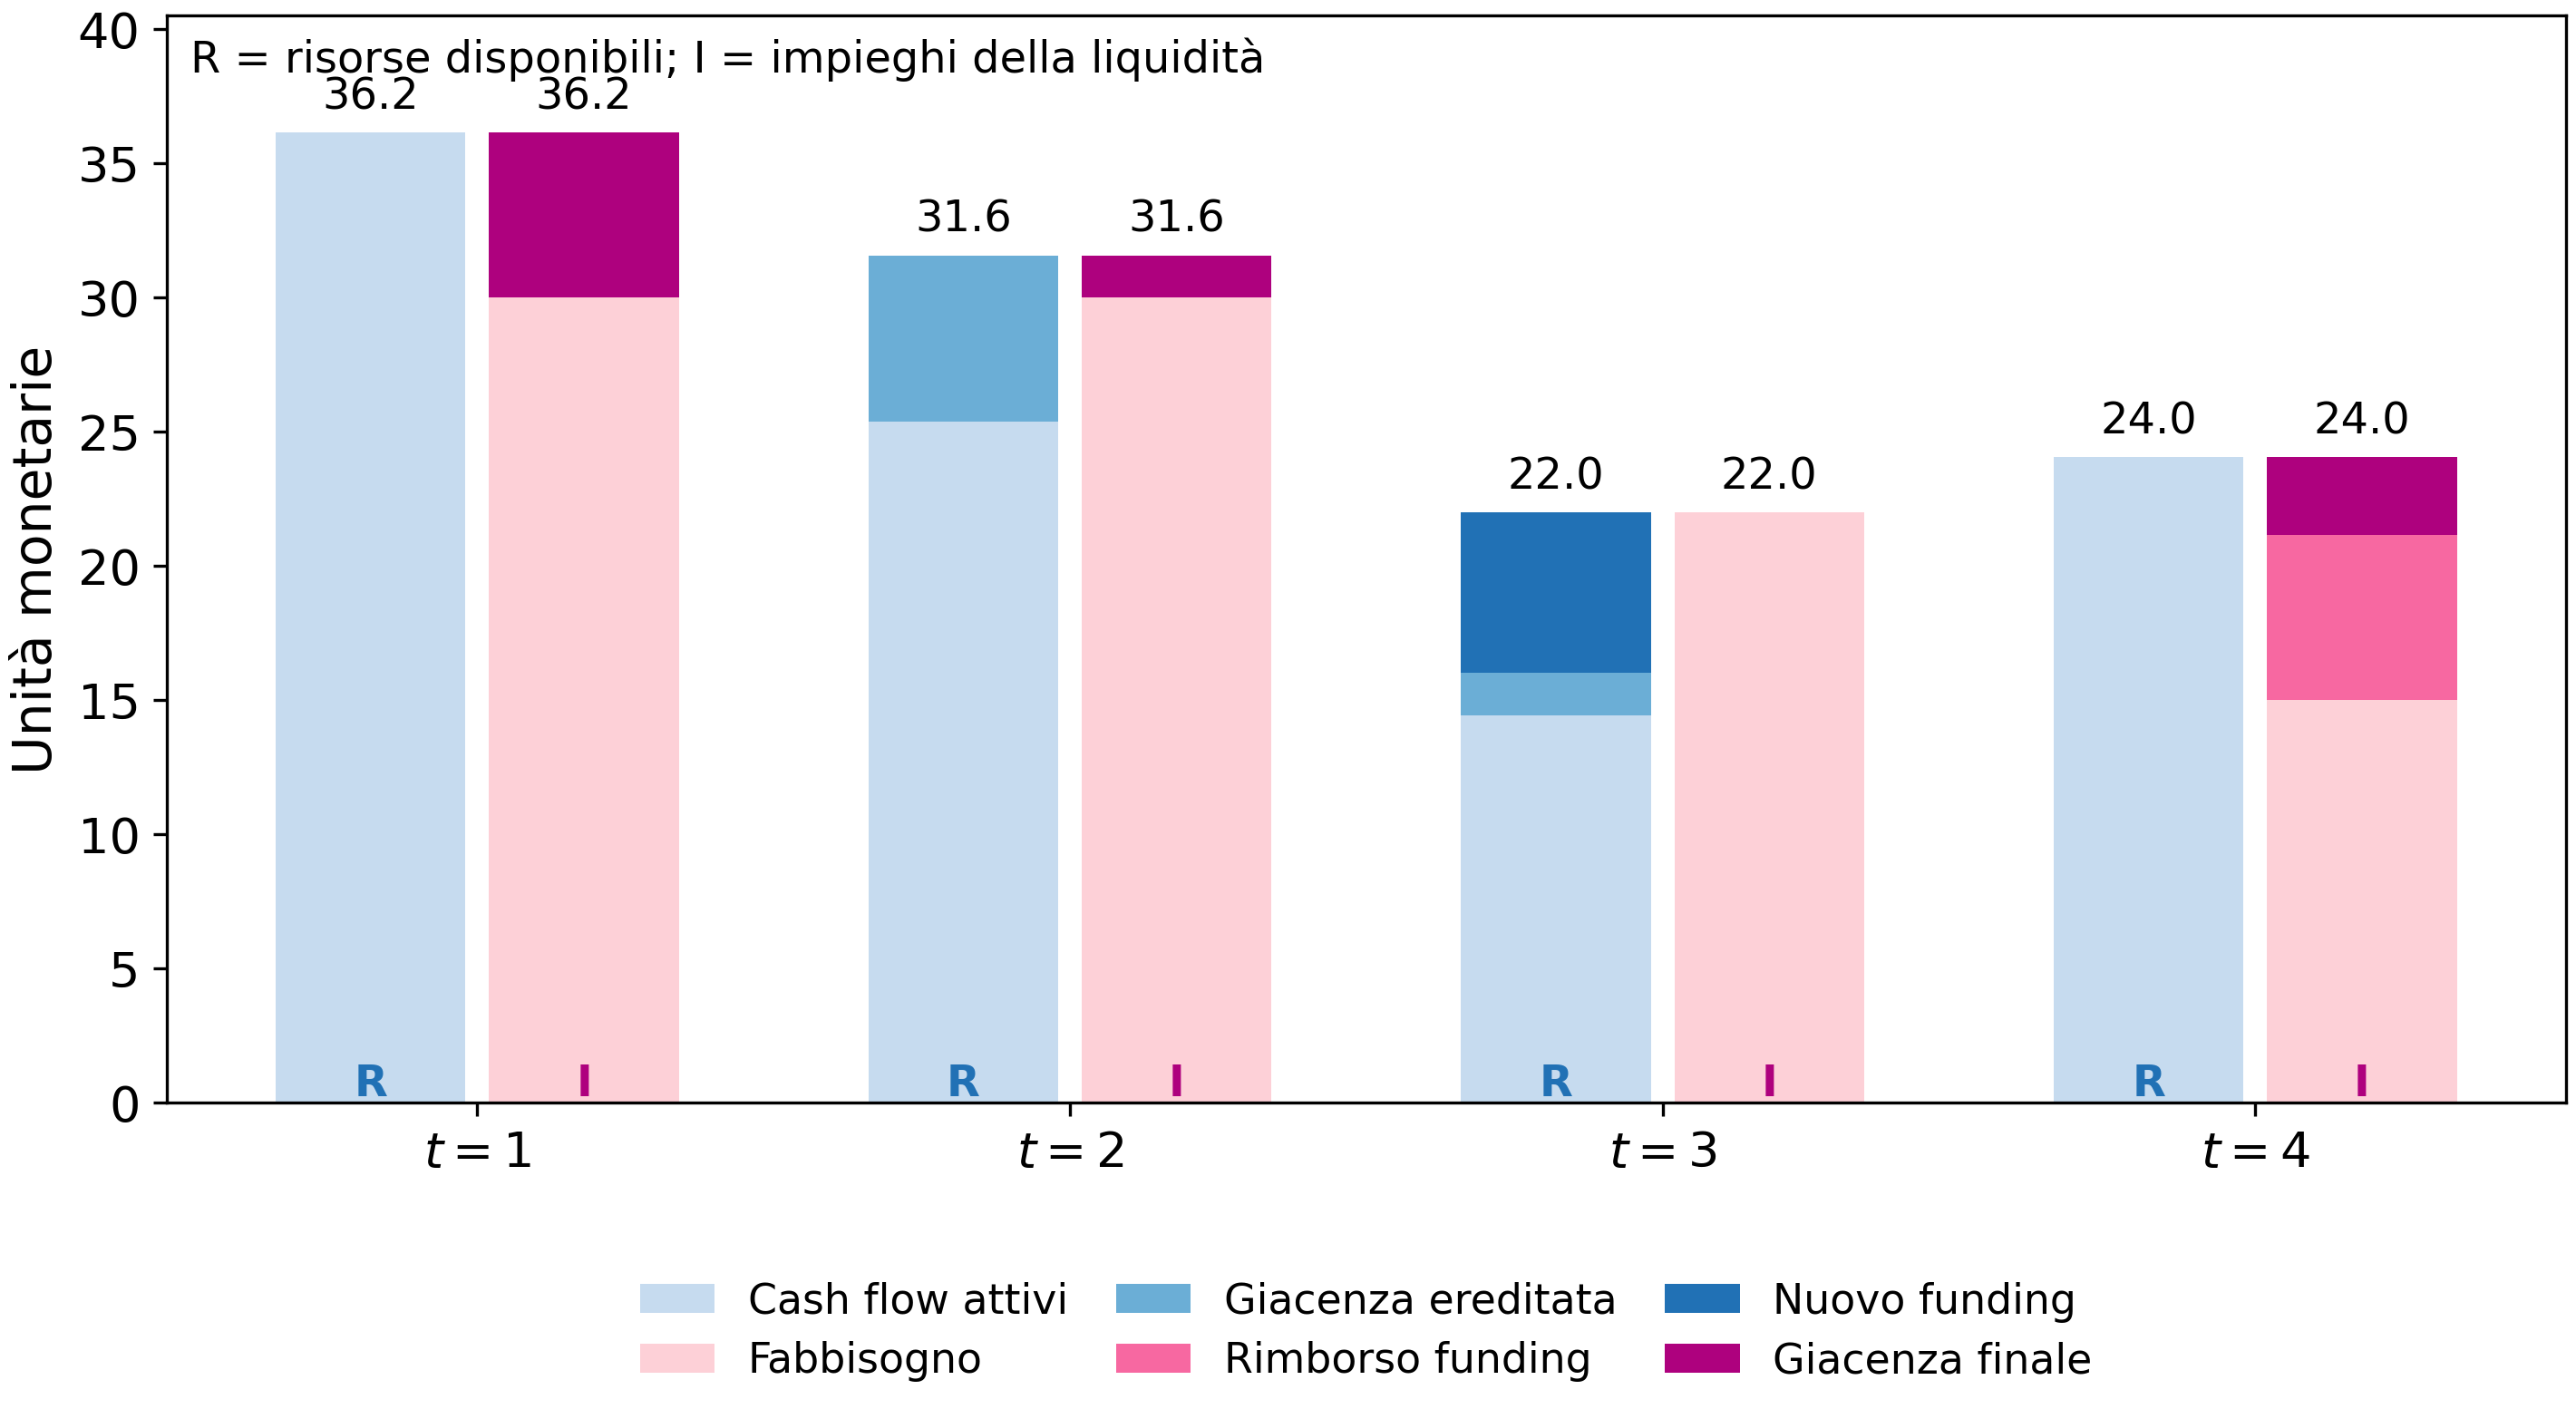
\includegraphics[width=0.94\textwidth]
{../graphics/Cap12_ALM_profili_ottimi.png}
\caption{Risorse e impieghi nelle quattro date della soluzione ottima del
caso SVB multiperiodale. La liquidit\`a accumulata trasferisce risorse verso
le date successive, mentre alla data $t=3$ il modello utilizza interamente
la capacit\`a di funding disponibile.}
\label{fig:cap12-alm-profili-ottimi}
\end{figure}

Infine, il contributo della composizione dell'attivo \`e

\[
c'x^*
\approx
3.7020,
\]

gli interessi sulle giacenze sono

\[
\sum_{t=1}^{3}r_tg_t^*
\approx
0.0402,
\]

e il costo del funding \`e

\[
\sum_{t=1}^{3}\rho_tu_t^*
=
0.1500.
\]

Pertanto,

\[
\Pi^*
\approx
3.5922.
\]

Il confronto diretto tra questo valore e il valore ottimo del problema
statico,

\[
z^{\mathrm{stat}}
\approx
3.765,
\]

non sarebbe tuttavia del tutto corretto, poich\'e la funzione obiettivo ALM
contiene anche interessi sulle giacenze e costi di funding. Per isolare
l'effetto sulla sola composizione dell'attivo \`e pi\`u informativo confrontare

\[
c'x^{\mathrm{stat}}
\approx
3.765
\]

con

\[
c'x^*
\approx
3.702.
\]

I vincoli prudenziali non risultano determinanti nella nuova soluzione:

\[
\ell'x^*
\approx
4.885
<
7,
\qquad
x_3^*=0<30.
\]

Al contrario, il limite

\[
u_3\leq6
\]

\`e raggiunto.

La sola osservazione dei vincoli attivi indica dove si concentra la scarsit\`a,
ma non ne misura ancora il valore economico. La domanda naturale diventa
quindi quale sia il valore marginale di una unit\`a aggiuntiva di risorse
disponibili nelle diverse date. Questo problema conduce direttamente
all'interpretazione duale dei bilanci temporali.

\section{Dualit\`a nell'ALM: il valore della liquidit\`a nelle diverse date}

\label{sec:cap12-dualita-alm}

Il Capitolo~\ref{cap:programmazione-lineare} ha mostrato che una variabile
duale consente di attribuire un valore marginale a una risorsa o a un
requisito del problema primale. Nel modello statico, un unico prezzo ombra
era associato al requisito aggregato di liquidit\`a.

Nel modello ALM la liquidit\`a non \`e invece concentrata in un solo vincolo.
Esiste un bilancio monetario per ciascuna data:

\[
a_t'x
+
(1+r_{t-1})g_{t-1}
+
u_t
-
(1+\rho_{t-1})u_{t-1}
-
g_t
=
d_t,
\]

con le opportune modifiche alla prima e all'ultima data.

La dualit\`a permette quindi di passare da un unico valore della liquidit\`a
a un profilo temporale di valori marginali.

\subsection{Il valore marginale dei bilanci temporali}

Associamo al bilancio della data $t$ una variabile duale

\[
\lambda_t\in\mathbb{R}.
\]

Poich\'e il vincolo di bilancio \`e un'uguaglianza, $\lambda_t$ non \`e
soggetta a un vincolo di segno.

Scrivendo il bilancio nella forma

\[
\text{risorse nette alla data }t=d_t,
\]

la convenzione adottata implica

\[
\frac{\partial\Pi^*}{\partial d_t}
=
-\lambda_t^*.
\]

Per una piccola variazione $\Delta d_t$ si ha quindi

\[
\Delta\Pi^*
\approx
-\lambda_t^*\,\Delta d_t.
\]

Se

\[
\lambda_t^*>0,
\]

un aumento unitario del fabbisogno alla data $t$ riduce localmente il
risultato ottimo di $\lambda_t^*$.

Equivalentemente, $\lambda_t^*$ misura il valore marginale di una unit\`a
aggiuntiva di liquidit\`a disponibile in quella stessa data.

Il passaggio rispetto al modello statico \`e quindi

\[
\boxed{
\text{un prezzo della liquidit\`a}
\quad\longrightarrow\quad
\text{un prezzo della liquidit\`a per ciascuna data}.
}
\]

\subsection{I valori duali nel caso SVB multiperiodale}

Per la soluzione della Sezione~\ref{sec:cap12-caso-svb-multiperiodale}, i
valori marginali dei quattro bilanci sono

\[
\lambda^*
\approx
\begin{pmatrix}
0.04524\\
0.04004\\
0.03383\\
0
\end{pmatrix}.
\]

La relazione tra posizione primale e valore marginale pu\`o essere riassunta
come segue:

\[
\begin{array}{c|c|c|c}
\hline
t & g_t^* & u_t^* & \lambda_t^*\\
\hline
1 & 6.152 & 0 & 0.04524\\
2 & 1.567 & 0 & 0.04004\\
3 & 0     & 6 & 0.03383\\
4 & 2.890 & - & 0\\
\hline
\end{array}
\]

Alla prima data, per esempio,

\[
\lambda_1^*
\approx
0.04524
\]

significa che un aumento marginale di una unit\`a del fabbisogno $d_1$
riduce il risultato ottimo di circa

\[
0.04524.
\]

Alla seconda e alla terza data il costo marginale rimane positivo, ma
diminuisce rispettivamente a

\[
0.04004
\]

e

\[
0.03383.
\]

Il risultato alla data finale richiede invece un'interpretazione specifica.

Poich\'e

\[
g_4^*
\approx
2.890>0
\]

e la giacenza terminale non riceve un valore nella funzione obiettivo, un
piccolo aumento di $d_4$ pu\`o essere assorbito semplicemente riducendo
$g_4$.

Localmente,

\[
\lambda_4^*=0.
\]

Questo non significa che la liquidit\`a alla data finale non abbia valore in
generale. Il risultato dipende dalla specificazione terminale del modello e
rimane valido finch\'e il margine rappresentato da $g_4^*$ non viene
esaurito.

\begin{figure}[htbp]
\centering
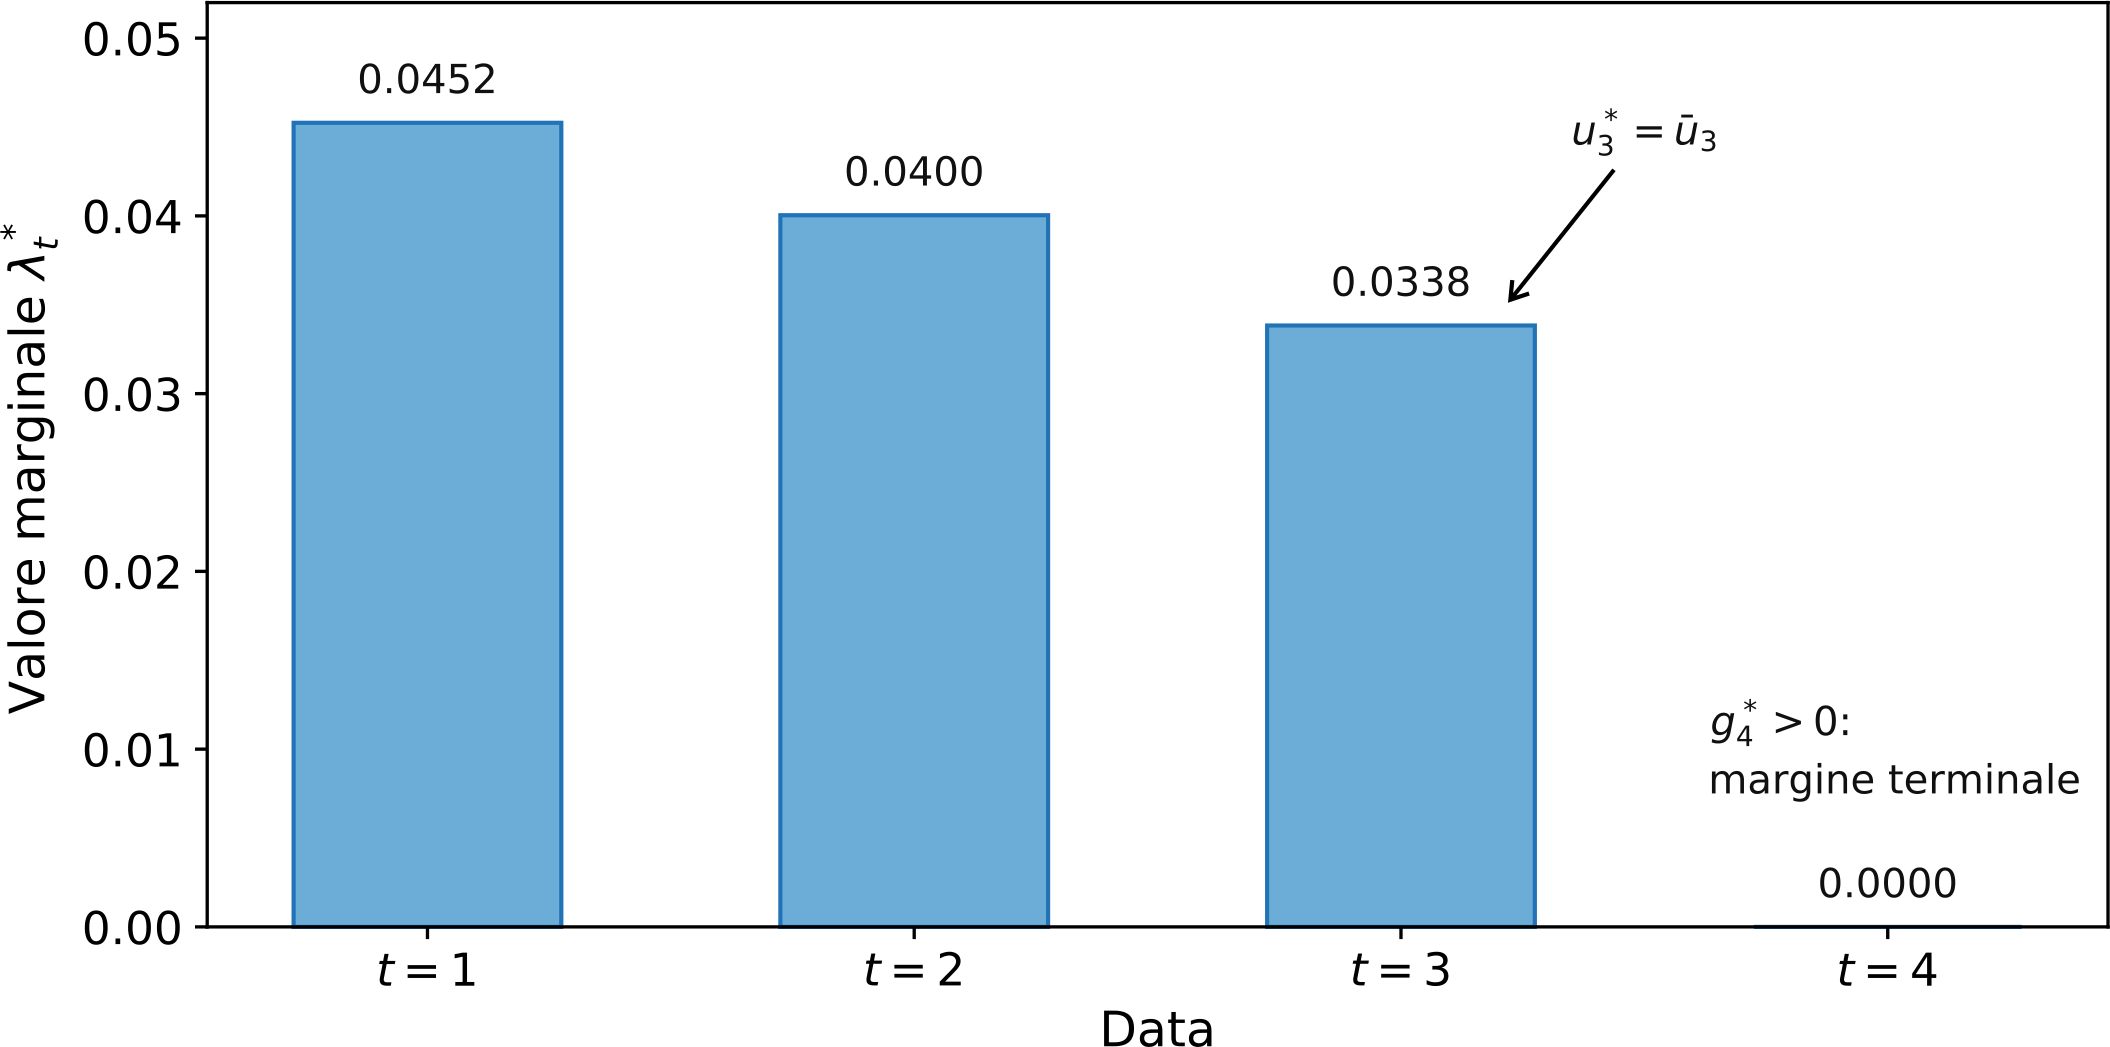
\includegraphics[width=0.88\textwidth]
{../graphics/Cap12_prezzi_ombra_scadenze.png}
\caption{Valore marginale della liquidit\`a nelle quattro date del caso SVB
multiperiodale. Il valore terminale \`e nullo localmente perch\'e la
soluzione presenta una giacenza finale positiva; alla data $t=3$ la banca
utilizza invece interamente la capacit\`a di funding disponibile.}
\label{fig:cap12-prezzi-ombra-scadenze}
\end{figure}

La Figura~\ref{fig:cap12-prezzi-ombra-scadenze} mostra un profilo decrescente
dei valori marginali. Tale andamento appartiene alla soluzione considerata e
non costituisce una propriet\`a generale dei modelli ALM: dipende dai cash
flow, dai fabbisogni, dai tassi, dai limiti di funding e dalla condizione
terminale.

\subsection{Il valore della capacit\`a di funding}

Un secondo valore duale rilevante riguarda il limite

\[
u_t\leq\bar u_t.
\]

Indichiamo con

\[
\lambda_{u,t}^*
\]

il valore marginale associato alla capacit\`a massima di funding. Localmente,

\[
\Delta\Pi^*
\approx
\lambda_{u,t}^*\,\Delta\bar u_t.
\]

Nella soluzione considerata,

\[
u_1^*<\bar u_1,
\qquad
u_2^*<\bar u_2,
\]

e i corrispondenti valori marginali sono nulli.

Alla terza data vale invece

\[
u_3^*
=
\bar u_3
=
6,
\]

e il valore duale associato al limite risulta

\[
\lambda_{u,3}^*
\approx
0.00883.
\]

Una piccola espansione della capacit\`a di funding disponibile alla data $3$
aumenterebbe quindi il valore ottimo di circa $0.00883$ per ogni unit\`a
aggiuntiva di capacit\`a.

Il risultato completa l'informazione fornita dalla soluzione primale:
l'uguaglianza

\[
u_3^*=\bar u_3
\]

individua una risorsa completamente utilizzata, mentre il corrispondente
valore duale misura quanto sarebbe economicamente utile, localmente,
allentarne il limite.

\section{Limiti del modello e passaggio all'incertezza}

\label{sec:cap12-limiti-incertezza}

Il modello sviluppato nelle sezioni precedenti permette di coordinare
composizione dell'attivo, liquidit\`a e funding lungo pi\`u date. La sua
struttura temporale \`e quindi pi\`u ricca di quella del problema statico del
Capitolo 11.

Rimane tuttavia un'ipotesi particolarmente forte: al tempo $0$ la banca
conosce l'intera traiettoria dei coefficienti che determineranno il problema
nelle date future.

\subsection{Che cosa significa deterministico}

Nel modello del capitolo sono noti al tempo $0$, tra gli altri,

\[
A^{\mathrm{CF}},
\qquad
d_t,
\qquad
r_t,
\qquad
\rho_t,
\qquad
\bar u_t.
\]

L'ipotesi deterministica non richiede che tali coefficienti siano costanti
nel tempo. Nel caso SVB multiperiodale, per esempio,

\[
r_1\neq r_2\neq r_3
\]

e anche la capacit\`a di funding varia:

\[
\bar u_1>\bar u_2>\bar u_3.
\]

Ci\`o che caratterizza il modello come deterministico \`e invece il fatto che
l'intero percorso

\[
\left\{
A^{\mathrm{CF}},
d_t,
r_t,
\rho_t,
\bar u_t
\right\}_{t=1}^{T}
\]

sia considerato noto quando il problema viene risolto.

Di conseguenza, la banca pu\`o determinare fin dal tempo $0$ l'intero piano

\[
x^*,
\qquad
g_1^*,\ldots,g_T^*,
\qquad
u_1^*,\ldots,u_{T-1}^*.
\]

Il modello risponde quindi alla domanda:

\[
\boxed{
\begin{array}{c}
\text{quale sarebbe il piano ottimo se la traiettoria futura}\\
\text{dei coefficienti fosse conosciuta?}
\end{array}
}
\]

Questa rappresentazione costituisce un benchmark utile, ma non descrive
completamente il problema decisionale affrontato da una banca reale.

\subsection{Quali elementi possono diventare incerti}

Nella realt\`a, alla data iniziale la banca non conosce con certezza le
condizioni che si manifesteranno nelle date successive.

Il vettore deterministico introdotto nella
Sezione~\ref{sec:cap12-ambiente-deterministico},

\[
\bar Z_t
=
(\bar R_t,\bar C_t,\bar F_t),
\]

pu\`o essere sostituito, in una rappresentazione incerta, da uno stato
economico-finanziario

\[
Z_t
=
(R_t,C_t,F_t).
\]

La distinzione \`e sostanziale. Nel primo caso

\[
\bar Z_t
\]

\`e un valore noto al momento della formulazione; nel secondo

\[
Z_t
\]

rappresenta uno stato futuro che non \`e ancora conosciuto al tempo $0$.

L'incertezza pu\`o quindi propagarsi ai coefficienti dell'ALM. In forma
schematica,

\[
Z_t
\quad\longrightarrow\quad
r_t,\ \rho_t,\ \bar u_t,
\]

e, quando economicamente appropriato, anche ai cash flow disponibili e ai
fabbisogni.

In particolare, il fabbisogno deterministico

\[
d_t
\]

pu\`o essere sostituito da una quantit\`a futura

\[
D_t,
\]

il cui valore dipende dalle condizioni che si realizzano.

La struttura concettuale discussa nella
Sezione~\ref{sec:cap12-stato-banca} suggerisce pi\`u precisamente

\[
D_t
=
d(Z_t,h_t),
\]

dove

\[
h_t
=
h(X_t,Z_t)
\]

dipende sia dall'ambiente esterno sia dallo stato della banca.

Non renderemo qui operative queste relazioni. Esse servono a individuare il
punto nel quale l'ipotesi deterministica dovr\`a essere abbandonata.

\subsection{Dal piano unico alle decisioni contingenti}

L'effetto pi\`u importante dell'incertezza riguarda la natura stessa delle
decisioni.

Nel modello deterministico il valore futuro di

\[
u_t
\]

pu\`o essere scelto gi\`a al tempo $0$, perch\'e i fabbisogni, i costi e la
capacit\`a di funding futuri sono noti.

In presenza di incertezza questa impostazione non \`e generalmente
appropriata. Il funding da utilizzare alla data $t$ dovrebbe poter dipendere
dalle condizioni effettivamente osservate a quella data.

Si passa quindi concettualmente da

\[
u_t
=
\text{numero fissato al tempo }0
\]

a una decisione del tipo

\[
u_t
=
u_t(\text{informazione disponibile alla data }t).
\]

La composizione iniziale $x$, invece, deve essere scelta prima di conoscere
gli stati futuri. Essa deve quindi tenere conto delle conseguenze che potranno
emergere lungo pi\`u evoluzioni possibili.

Il passaggio fondamentale pu\`o essere sintetizzato come

\[
\boxed{
\begin{array}{ccc}
\text{ALM deterministico}
&
\longrightarrow
&
\text{ALM sotto incertezza}
\\[4pt]
\text{una traiettoria nota}
&&
\text{pi\`u evoluzioni possibili}
\\[4pt]
\text{un piano fissato al tempo }0
&&
\text{decisioni compatibili con l'informazione disponibile}.
\end{array}
}
\]

Anche i valori duali ottenuti nelle sezioni precedenti devono essere letti
alla luce di questa distinzione. Essi misurano valori marginali
\emph{condizionati alla traiettoria deterministica assunta}: non incorporano
da soli il rischio che tassi, fabbisogni o disponibilit\`a di funding seguano
percorsi differenti.

Il modello deterministico rimane quindi un riferimento essenziale. Permette
di isolare la struttura dei bilanci intertemporali, identificare le date nelle
quali le risorse risultano scarse e attribuire loro un valore marginale.

Il passo successivo consiste nel mantenere questa struttura temporale
abbandonando l'ipotesi di conoscenza perfetta del futuro.

\section{Esercizi svolti}

\label{sec:cap12-esercizi-svolti}

Gli esercizi seguenti consolidano tre passaggi centrali del capitolo:
la formulazione di un problema ALM, la verifica della fattibilit\`a
intertemporale e l'interpretazione dei valori duali.

\begin{exercise}[Dalla descrizione del problema alla formulazione]

\label{ex:cap12-formulazione-alm-solver}

Una banca dispone al tempo $0$ di $50$ unit\`a monetarie, che devono essere
interamente allocate tra tre classi di attivo.

La prima classe rappresenta cassa e riserve. Produce un contributo economico
pari all'1\% dell'investimento e l'intero ammontare investito diventa
disponibile come liquidit\`a alla data $1$.

La seconda classe \`e costituita da titoli a breve scadenza. Produce un
contributo economico del $2.5\%$; il $60\%$ dell'investimento iniziale diventa
disponibile alla data $1$ e il restante $40\%$ alla data $2$.

La terza classe \`e costituita da prestiti. Produce un contributo economico
del $4.5\%$; il $10\%$ dell'investimento iniziale diventa disponibile alla
data $1$, il $30\%$ alla data $2$ e il restante $60\%$ alla data $3$.

I fabbisogni di liquidit\`a alle tre date sono rispettivamente

\[
25,\qquad18,\qquad12.
\]

La liquidit\`a non utilizzata alla data $1$ pu\`o essere trasferita alla data
$2$ con un rendimento dello $0.5\%$; quella non utilizzata alla data $2$ pu\`o
essere trasferita alla data $3$ con un rendimento dello $0.6\%$.

La banca pu\`o inoltre raccogliere funding alla data $1$ fino a un massimo di
$4$ unit\`a, con costo dell'1.5\%, e alla data $2$ fino a un massimo di $3$
unit\`a, con costo del $2\%$. Il funding raccolto in una data deve essere
rimborsato alla data successiva.

In uno scenario di stress, le perdite unitarie associate alle tre classi di
attivo sono rispettivamente

\[
0,\qquad0.03,\qquad0.08,
\]

e la perdita complessiva non pu\`o superare $2.6$.

Infine, l'investimento nei prestiti non pu\`o superare $25$ unit\`a.

A partire esclusivamente da queste informazioni:

\begin{enumerate}

\item individuare le variabili decisionali;

\item costruire i vettori e la matrice dei parametri necessari;

\item formulare matematicamente la funzione obiettivo;

\item scrivere il vincolo sulle risorse iniziali, i tre bilanci di liquidit\`a,
i vincoli prudenziali, i limiti sul funding e le condizioni di non negativit\`a;

\item raccogliere tutte le variabili in un unico vettore $z$ e scrivere il
problema nella forma matriciale necessaria per l'utilizzo di un solver LP:

\[
\min\;\widetilde c'z,
\qquad
A_{\mathrm{ub}}z\leq b_{\mathrm{ub}},
\qquad
A_{\mathrm{eq}}z=b_{\mathrm{eq}},
\]

specificando inoltre i bounds delle variabili.
\end{enumerate}

\end{exercise}

\noindent
\textbf{Soluzione.}

\begin{enumerate}

\item \textbf{Variabili decisionali.}

Indichiamo con

\[
x_1,\qquad x_2,\qquad x_3
\]

gli importi investiti al tempo $0$ rispettivamente in cassa e riserve,
titoli a breve scadenza e prestiti.

Le giacenze di liquidit\`a residue alle tre date sono

\[
g_1,\qquad g_2,\qquad g_3,
\]

mentre il funding raccolto alle prime due date \`e rappresentato da

\[
u_1,\qquad u_2.
\]

Non viene introdotto nuovo funding alla data finale, poich\'e il relativo
rimborso cadrebbe oltre l'orizzonte del modello.

Tutte le variabili sono non negative:

\[
x_j\geq0,
\qquad
j=1,2,3,
\]

\[
g_t\geq0,
\qquad
t=1,2,3,
\]

\[
u_t\geq0,
\qquad
t=1,2.
\]


\item \textbf{Costruzione dei parametri.}

Dalla descrizione delle tre classi di attivo si ricava il vettore dei
contributi economici unitari

\[
c
=
\begin{pmatrix}
0.010\\
0.025\\
0.045
\end{pmatrix}.
\]

I profili temporali con cui le risorse investite nelle tre classi diventano
disponibili determinano la matrice dei cash flow

\[
A^{\mathrm{CF}}
=
\begin{pmatrix}
1.00 & 0.60 & 0.10\\
0    & 0.40 & 0.30\\
0    & 0    & 0.60
\end{pmatrix}.
\]

Il vettore dei fabbisogni \`e

\[
d
=
\begin{pmatrix}
25\\
18\\
12
\end{pmatrix}.
\]

I rendimenti delle giacenze sono

\[
r_1=0.005,
\qquad
r_2=0.006,
\]

mentre i costi del funding sono

\[
\rho_1=0.015,
\qquad
\rho_2=0.020.
\]

La capacit\`a massima di funding \`e

\[
\bar u_1=4,
\qquad
\bar u_2=3.
\]

Il vettore delle perdite unitarie nello scenario di stress \`e

\[
\ell
=
\begin{pmatrix}
0\\
0.03\\
0.08
\end{pmatrix},
\]

con limite complessivo

\[
K=2.6.
\]

Infine, il limite di concentrazione sui prestiti \`e

\[
x_3\leq25.
\]


\item \textbf{Funzione obiettivo.}

In forma simbolica, per un orizzonte con $T=3$ date future, la funzione
obiettivo \`e

\[
\max\;
\Pi(x,g,u)
=
c'x
+
\sum_{t=1}^{2}r_tg_t
-
\sum_{t=1}^{2}\rho_tu_t.
\]

Sostituendo i valori numerici si ottiene

\[
\boxed{
\max\;
0.010x_1
+
0.025x_2
+
0.045x_3
+
0.005g_1
+
0.006g_2
-
0.015u_1
-
0.020u_2.
}
\]


\item \textbf{Vincoli del modello ALM.}

Le risorse iniziali devono essere interamente allocate:

\[
x_1+x_2+x_3=50.
\]

Alla prima data sono disponibili i cash flow prodotti dagli attivi e il
funding eventualmente raccolto in $t=1$. Il bilancio di liquidit\`a \`e

\[
x_1
+
0.60x_2
+
0.10x_3
+
u_1
=
25+g_1,
\]

ovvero

\[
x_1
+
0.60x_2
+
0.10x_3
+
u_1
-
g_1
=
25.
\]

Alla seconda data diventano disponibili i nuovi cash flow degli attivi, la
giacenza precedente capitalizzata e il nuovo funding. Deve inoltre essere
rimborsato il funding raccolto alla prima data:

\[
0.40x_2
+
0.30x_3
+
1.005g_1
+
u_2
=
18
+
1.015u_1
+
g_2.
\]

Pertanto,

\[
0.40x_2
+
0.30x_3
+
1.005g_1
+
u_2
-
1.015u_1
-
g_2
=
18.
\]

Alla data finale non viene raccolto nuovo funding:

\[
0.60x_3
+
1.006g_2
=
12
+
1.020u_2
+
g_3,
\]

ossia

\[
0.60x_3
+
1.006g_2
-
1.020u_2
-
g_3
=
12.
\]

Il vincolo sulla perdita nello scenario di stress \`e

\[
0.03x_2+0.08x_3\leq2.6.
\]

Il limite di concentrazione sui prestiti \`e

\[
x_3\leq25.
\]

I limiti sul funding sono

\[
0\leq u_1\leq4,
\qquad
0\leq u_2\leq3.
\]

Infine,

\[
x_1,x_2,x_3\geq0,
\qquad
g_1,g_2,g_3\geq0.
\]

Il programma lineare completo \`e quindi

\[
\begin{array}{ll}

\max
&
\displaystyle
0.010x_1
+
0.025x_2
+
0.045x_3
\\
& +
0.005g_1
+
0.006g_2
-
0.015u_1
-
0.020u_2
\\[8pt]

\mbox{soggetto a}
&
x_1+x_2+x_3=50,
\\[6pt]

&
x_1+0.60x_2+0.10x_3+u_1-g_1=25,
\\[6pt]

&
0.40x_2+0.30x_3+1.005g_1
+u_2-1.015u_1-g_2=18,
\\[6pt]

&
0.60x_3+1.006g_2-1.020u_2-g_3=12,
\\[6pt]

&
0.03x_2+0.08x_3\leq2.6,
\\[6pt]

&
x_3\leq25,
\\[6pt]

&
0\leq u_1\leq4,
\qquad
0\leq u_2\leq3,
\\[6pt]

&
x_1,x_2,x_3,g_1,g_2,g_3\geq0.
\end{array}
\]


\item \textbf{Forma matriciale per il solver.}

Raccogliamo le variabili secondo l'ordine

\[
z
=
\begin{pmatrix}
x_1&
x_2&
x_3&
g_1&
g_2&
g_3&
u_1&
u_2
\end{pmatrix}'.
\]

Rispetto a questo ordinamento, il vettore dei coefficienti della funzione
obiettivo in massimizzazione \`e

\[
c^{\mathrm{ALM}}
=
\begin{pmatrix}
0.010\\
0.025\\
0.045\\
0.005\\
0.006\\
0\\
-0.015\\
-0.020
\end{pmatrix}.
\]

Poich\'e il solver \texttt{scipy.optimize.linprog} utilizza una formulazione
in minimizzazione, si pone

\[
\widetilde c
=
-c^{\mathrm{ALM}},
\]

e quindi

\[
\widetilde c
=
\begin{pmatrix}
-0.010\\
-0.025\\
-0.045\\
-0.005\\
-0.006\\
0\\
0.015\\
0.020
\end{pmatrix}.
\]

Il problema passato al solver ha pertanto funzione obiettivo

\[
\min\;\widetilde c'z.
\]

Il vincolo sulle risorse iniziali e i tre bilanci temporali sono uguaglianze.
Essi possono essere raccolti nella matrice

\[
A_{\mathrm{eq}}
=
\begin{pmatrix}
1 & 1    & 1    & 0     & 0     & 0  & 0      & 0\\
1 & 0.60 & 0.10 & -1    & 0     & 0  & 1      & 0\\
0 & 0.40 & 0.30 & 1.005 & -1    & 0  & -1.015 & 1\\
0 & 0    & 0.60 & 0     & 1.006 & -1 & 0      & -1.020
\end{pmatrix},
\]

con

\[
b_{\mathrm{eq}}
=
\begin{pmatrix}
50\\
25\\
18\\
12
\end{pmatrix}.
\]

I due vincoli espressi come disuguaglianze sono

\[
0.03x_2+0.08x_3\leq2.6
\]

e

\[
x_3\leq25.
\]

Pertanto,

\[
A_{\mathrm{ub}}
=
\begin{pmatrix}
0 & 0.03 & 0.08 & 0 & 0 & 0 & 0 & 0\\
0 & 0    & 1    & 0 & 0 & 0 & 0 & 0
\end{pmatrix},
\]

e

\[
b_{\mathrm{ub}}
=
\begin{pmatrix}
2.6\\
25
\end{pmatrix}.
\]

Infine, i limiti delle variabili sono

\[
\begin{array}{c|c}
\text{variabili} & \text{bounds}\\
\hline
x_1,x_2,x_3 & [0,+\infty)\\
g_1,g_2,g_3 & [0,+\infty)\\
u_1 & [0,4]\\
u_2 & [0,3].
\end{array}
\]

La formulazione da trasmettere al solver \`e quindi completamente
specificata da

\[
\boxed{
\begin{array}{c}
\displaystyle
\min\;\widetilde c'z
\\[6pt]
A_{\mathrm{eq}}z=b_{\mathrm{eq}},
\\[4pt]
A_{\mathrm{ub}}z\leq b_{\mathrm{ub}},
\\[4pt]
\underline z\leq z\leq\overline z.
\end{array}
}
\]

Il passaggio decisivo non consiste nell'applicazione del solver, ma nella
traduzione coerente della descrizione finanziaria in variabili, coefficienti
e vincoli. Una volta costruita correttamente questa rappresentazione, il
problema \`e un programma lineare standard e pu\`o essere risolto
numericamente senza ulteriori modifiche alla sua struttura economica.

\end{enumerate}


\begin{exercise}[Fattibilit\`a temporale e limite al funding]

\label{ex:cap12-fattibilita-funding}

Una banca ha investito al tempo $0$ in due classi di attivo secondo la
composizione

\[
x=
\begin{pmatrix}
20\\
20
\end{pmatrix}.
\]

La distribuzione temporale dei cash flow prodotti dagli attivi \`e descritta
dalla matrice

\[
A^{\mathrm{CF}}
=
\begin{pmatrix}
0.70 & 0.10\\
0.30 & 0.30\\
0    & 0.60
\end{pmatrix}.
\]

I fabbisogni di liquidit\`a alle tre date sono

\[
d'
=
(15,\;14,\;8).
\]

La liquidit\`a residua alla prima data pu\`o essere trasferita alla seconda
con rendimento

\[
r_1=0.005.
\]

Si assume che non venga raccolto funding alla prima data,

\[
u_1=0,
\]

mentre alla seconda data la banca pu\`o ricorrere a funding che dovr\`a essere
rimborsato alla data finale con costo

\[
\rho_2=0.020.
\]

In condizioni ordinarie la capacit\`a di funding alla seconda data \`e

\[
\bar u_2=3.
\]

\begin{enumerate}

\item Calcolare il profilo temporale dei cash flow prodotto dagli attivi.

\item Verificare se la composizione assegnata permette di soddisfare i
fabbisogni alle tre date senza ricorrere al funding.

\item Determinare il funding minimo necessario alla seconda data e calcolare
la giacenza terminale risultante.

\item Supporre ora che la capacit\`a massima di funding alla seconda data si
riduca a

\[
\bar u_2=0.8.
\]

Stabilire se il piano rimane ammissibile e interpretare il risultato.

\end{enumerate}

\end{exercise}

\noindent
\textbf{Soluzione.}

\begin{enumerate}

\item Il profilo dei cash flow \`e

\[
A^{\mathrm{CF}}x
=
\begin{pmatrix}
0.70 & 0.10\\
0.30 & 0.30\\
0    & 0.60
\end{pmatrix}
\begin{pmatrix}
20\\
20
\end{pmatrix}
=
\begin{pmatrix}
16\\
12\\
12
\end{pmatrix}.
\]

\item Alla prima data, ponendo $u_1=0$,

\[
16=15+g_1,
\]

da cui

\[
g_1=1.
\]

Alla seconda data, in assenza di funding, le risorse disponibili sarebbero

\[
12+1.005(1)
=
13.005.
\]

Il fabbisogno \`e invece

\[
d_2=14.
\]

Pertanto

\[
13.005<14
\]

e la composizione non \`e temporalmente fattibile senza funding.

Il punto importante \`e che l'insufficienza emerge alla seconda data:
non pu\`o essere compensata utilizzando anticipatamente il cash flow pari a
$12$ che sar\`a disponibile soltanto alla data successiva.

\item Ponendo $g_2=0$, il bilancio della seconda data richiede

\[
12
+
1.005(1)
+
u_2
=
14.
\]

Il funding minimo \`e quindi

\[
u_2
=
14-13.005
=
0.995.
\]

Alla data finale il rimborso dovuto \`e

\[
1.020(0.995)
=
1.0149.
\]

Il bilancio terminale diventa

\[
12
=
8
+
1.0149
+
g_3,
\]

da cui

\[
g_3
=
2.9851.
\]

Il funding anticipa quindi $0.995$ unit\`a alla seconda data e genera alla
terza un rimborso pari a $1.0149$.

\item Se

\[
\bar u_2=0.8,
\]

il funding massimo disponibile sarebbe inferiore al fabbisogno minimo

\[
u_2^{\min}=0.995.
\]

La composizione considerata diventerebbe quindi non ammissibile:

\[
\bar u_2<u_2^{\min}.
\]

\end{enumerate}

L'esercizio distingue due concetti che non devono essere confusi:
l'esistenza di risorse lungo l'intero orizzonte e la loro disponibilit\`a
nella data nella quale devono essere utilizzate.


\begin{exercise}[Interpretazione dei valori duali]

\label{ex:cap12-valori-duali}

Nel caso SVB multiperiodale della
Sezione~\ref{sec:cap12-caso-svb-multiperiodale}, i valori marginali associati
ai quattro bilanci temporali sono

\[
\lambda^*
\approx
\begin{pmatrix}
0.04524\\
0.04004\\
0.03383\\
0
\end{pmatrix}.
\]

Il valore duale associato al limite

\[
u_3\leq\bar u_3
\]

\`e inoltre

\[
\lambda_{u,3}^*
\approx
0.00883.
\]

Si assuma che le variazioni considerate siano sufficientemente piccole da
non modificare la struttura della soluzione ottima.

\begin{enumerate}

\item Stimare l'effetto sul valore ottimo di un aumento

\[
\Delta d_2=0.5.
\]

\item Interpretare il risultato

\[
\lambda_4^*=0
\]

sapendo che

\[
g_4^*\approx2.890.
\]

\item Stimare l'effetto di un aumento unitario della capacit\`a di funding
alla terza data.

\item Spiegare perch\'e queste valutazioni devono essere interpretate
localmente.

\end{enumerate}

\end{exercise}

\noindent
\textbf{Soluzione.}

\begin{enumerate}

\item Per una piccola variazione del fabbisogno vale

\[
\Delta\Pi^*
\approx
-\lambda_2^*\,\Delta d_2.
\]

Pertanto

\[
\Delta\Pi^*
\approx
-0.04004(0.5)
=
-0.02002.
\]

Un aumento di mezzo punto del fabbisogno alla seconda data riduce quindi
localmente il valore ottimo di circa $0.020$.

\item Il risultato

\[
\lambda_4^*=0
\]

non significa che la liquidit\`a alla data finale sia priva di significato
finanziario.

Nella soluzione considerata esiste infatti una giacenza terminale positiva:

\[
g_4^*\approx2.890.
\]

Un piccolo aumento di $d_4$ pu\`o essere assorbito riducendo questa giacenza,
senza richiedere una modifica della composizione dell'attivo o del piano di
funding e senza modificare localmente la funzione obiettivo.

Il valore marginale nullo riflette quindi l'esistenza di un margine terminale
nella soluzione considerata.

\item Per il limite sulla capacit\`a di funding vale localmente

\[
\Delta\Pi^*
\approx
\lambda_{u,3}^*
\Delta\bar u_3.
\]

Con

\[
\Delta\bar u_3=1
\]

si ottiene

\[
\Delta\Pi^*
\approx
0.00883.
\]

Una unit\`a aggiuntiva di capacit\`a di funding alla terza data aumenterebbe
quindi il risultato massimo di circa $0.00883$.

\item I valori duali descrivono la pendenza locale della funzione valore
rispetto ai termini noti o ai limiti considerati.

Se una variazione sufficientemente ampia modifica i vincoli determinanti
della soluzione, anche i corrispondenti valori marginali possono cambiare.
Non \`e quindi corretto utilizzare indefinitamente lo stesso prezzo ombra
per variazioni arbitrarie dei parametri.

\end{enumerate}

Il confronto tra soluzione primale e valori duali mette in evidenza due
informazioni complementari: il primale mostra come vengono impiegate le
risorse disponibili, mentre il duale quantifica il valore marginale di una
variazione dei requisiti o delle risorse scarse.

\section{Esercizi proposti}

\label{sec:cap12-esercizi-proposti}


\begin{exercise}[Cash flow aggregati e distribuzione temporale]

\label{ex:cap12-proposto-cashflow-temporali}

Una banca considera tre classi di attivo. La matrice dei cash flow \`e

\[
A^{\mathrm{CF}}
=
\begin{pmatrix}
0.80 & 0.30 & 0.10\\
0.20 & 0.40 & 0.30\\
0    & 0.30 & 0.60
\end{pmatrix},
\]

e la composizione iniziale \`e

\[
x'
=
(10,\;20,\;30).
\]

I fabbisogni sono

\[
d'
=
(16,\;21,\;18).
\]

Si assumano, per semplicit\`a,

\[
r_1=r_2=0.
\]

Alla seconda data la banca pu\`o raccogliere funding al tasso

\[
\rho_2=0.02.
\]

\begin{enumerate}

\item Calcolare il profilo temporale

\[
A^{\mathrm{CF}}x.
\]

\item Verificare che il cash flow complessivo prodotto lungo l'orizzonte
coincida con l'ammontare inizialmente investito.

\item Stabilire se i fabbisogni possono essere soddisfatti senza funding,
tenendo conto del trasferimento delle giacenze tra date consecutive.

\item Determinare il funding minimo necessario alla seconda data e la
giacenza terminale risultante.

\item Spiegare perch\'e il confronto tra

\[
\sum_t d_t
\]

e il cash flow complessivo dell'attivo non \`e sufficiente per stabilire
l'ammissibilit\`a del piano.

\end{enumerate}

\end{exercise}

\noindent
\textit{Risultati:}

\[
A^{\mathrm{CF}}x
=
\begin{pmatrix}
17\\
19\\
24
\end{pmatrix},
\qquad
\sum_{t=1}^{3}(A^{\mathrm{CF}}x)_t=60.
\]

Alla prima data

\[
g_1=1.
\]

Alla seconda data rimane un deficit pari a $1$, per cui il funding minimo
\`e

\[
u_2=1.
\]

Tenendo conto del rimborso alla data finale,

\[
g_3=24-18-1.02=4.98.
\]


\begin{exercise}[Due portafogli con diversa struttura temporale]

\label{ex:cap12-proposto-confronto-portafogli}

Si consideri la matrice

\[
A^{\mathrm{CF}}
=
\begin{pmatrix}
0.90 & 0.40 & 0.10\\
0.10 & 0.40 & 0.30\\
0    & 0.20 & 0.60
\end{pmatrix}
\]

e i due portafogli

\[
x^{(A)}
=
\begin{pmatrix}
20\\
20\\
10
\end{pmatrix},
\qquad
x^{(B)}
=
\begin{pmatrix}
10\\
20\\
20
\end{pmatrix}.
\]

Entrambi utilizzano risorse iniziali pari a

\[
A_0=50.
\]

I fabbisogni sono

\[
d'
=
(22,\;16,\;10).
\]

I parametri finanziari sono

\[
r_1=0.004,
\qquad
r_2=0.005,
\]

\[
\rho_1=0.014,
\qquad
\rho_2=0.018,
\]

con

\[
\bar u_1=5,
\qquad
\bar u_2=4.
\]

\begin{enumerate}

\item Calcolare i profili

\[
A^{\mathrm{CF}}x^{(A)}
\qquad\text{e}\qquad
A^{\mathrm{CF}}x^{(B)}.
\]

\item Verificare se il portafoglio $A$ pu\`o soddisfare i tre fabbisogni
senza ricorrere al funding.

\item Per il portafoglio $B$, determinare il funding minimo necessario alla
prima data.

\item Verificare se la capacit\`a massima di funding alla seconda data
permette di proseguire il piano.

\item Interpretare la differenza tra i due portafogli dal punto di vista
dell'ALM.

\end{enumerate}

\end{exercise}

\noindent
\textit{Risultati:}

\[
A^{\mathrm{CF}}x^{(A)}
=
\begin{pmatrix}
27\\
13\\
10
\end{pmatrix},
\qquad
A^{\mathrm{CF}}x^{(B)}
=
\begin{pmatrix}
19\\
15\\
16
\end{pmatrix}.
\]

Il portafoglio $A$ \`e finanziariamente ammissibile senza funding.

Per il portafoglio $B$ occorre alla prima data

\[
u_1=3.
\]

Alla seconda data il funding minimo richiesto \`e circa

\[
u_2=4.042,
\]

ma

\[
\bar u_2=4.
\]

Il portafoglio $B$ non \`e quindi ammissibile.


\begin{exercise}[Formulazione completa di un problema ALM]

\label{ex:cap12-proposto-formulazione-completa}

Una banca dispone di

\[
A_0=50
\]

unit\`a monetarie e pu\`o scegliere tra tre classi di attivo.

I parametri dell'attivo sono

\[
\begin{array}{c|cc}
\hline
j & c_j & \ell_j\\
\hline
1 & 0.015 & 0\\
2 & 0.030 & 0.04\\
3 & 0.045 & 0.10\\
\hline
\end{array}
\]

e

\[
A^{\mathrm{CF}}
=
\begin{pmatrix}
0.90 & 0.40 & 0.10\\
0.10 & 0.40 & 0.30\\
0    & 0.20 & 0.60
\end{pmatrix}.
\]

I parametri temporali sono

\[
\begin{array}{c|cccc}
\hline
t & d_t & r_t & \rho_t & \bar u_t\\
\hline
1 & 20 & 0.004 & 0.014 & 5\\
2 & 18 & 0.005 & 0.018 & 4\\
3 & 10 & -     & -     & -\\
\hline
\end{array}
\]

e il limite alla perdita sotto stress \`e

\[
\ell'x\leq3.2.
\]

La terza classe di attivo non pu\`o inoltre superare

\[
x_3\leq20.
\]

\begin{enumerate}

\item Individuare tutte le variabili decisionali.

\item Scrivere la funzione obiettivo prima in forma simbolica e poi in forma
numerica.

\item Scrivere il vincolo sulle risorse iniziali.

\item Scrivere i tre bilanci di liquidit\`a prima in forma simbolica e poi
sostituendo i coefficienti numerici.

\item Completare il programma lineare con i limiti di funding, il vincolo di
stress, il limite di concentrazione e le condizioni di non negativit\`a.

\item Indicare quali coefficienti del modello potrebbero dipendere
dall'ambiente economico-finanziario

\[
\bar Z_t=(\bar R_t,\bar C_t,\bar F_t).
\]

\end{enumerate}

\end{exercise}

\noindent
\textit{Risultati di controllo:} le variabili sono

\[
x_1,x_2,x_3,
\qquad
g_1,g_2,g_3,
\qquad
u_1,u_2.
\]

La funzione obiettivo numerica \`e

\[
\max\;
0.015x_1+0.030x_2+0.045x_3
+0.004g_1+0.005g_2
-0.014u_1-0.018u_2.
\]

Il primo bilancio \`e

\[
0.90x_1+0.40x_2+0.10x_3+u_1-g_1=20.
\]


\begin{exercise}[Sensitivit\`a dei fabbisogni e della capacit\`a di funding]

\label{ex:cap12-proposto-sensitivita}

Nel caso SVB multiperiodale sono stati ottenuti i valori marginali

\[
\lambda^*
\approx
\begin{pmatrix}
0.04524\\
0.04004\\
0.03383\\
0
\end{pmatrix}
\]

per i quattro bilanci temporali.

Il valore duale del limite sulla capacit\`a di funding alla terza data \`e

\[
\lambda_{u,3}^*
\approx
0.00883.
\]

Si considerino variazioni sufficientemente piccole da non modificare la
struttura della soluzione ottima.

\begin{enumerate}

\item Stimare la variazione del valore ottimo se

\[
d_1
\]

aumenta di $0.4$.

\item Ripetere il calcolo per un aumento di $0.4$ di $d_3$.

\item Stimare il beneficio di un aumento pari a $0.5$ della capacit\`a

\[
\bar u_3.
\]

\item Spiegare perch\'e un piccolo aumento di $d_4$ ha valore marginale nullo
nella soluzione considerata.

\item Stabilire se sarebbe corretto utilizzare

\[
\lambda_4^*=0
\]

per valutare un aumento di $d_4$ pari a $4$ unit\`a, sapendo che

\[
g_4^*\approx2.890.
\]

\end{enumerate}

\end{exercise}

\noindent
\textit{Risultati:}

\[
\Delta\Pi^*
\approx
-0.04524(0.4)
=
-0.01810
\]

per la prima data,

\[
\Delta\Pi^*
\approx
-0.03383(0.4)
=
-0.01353
\]

per la terza data, e

\[
\Delta\Pi^*
\approx
0.00883(0.5)
=
0.00442
\]

per l'espansione della capacit\`a di funding.

Il valore $\lambda_4^*=0$ non pu\`o essere esteso automaticamente a una
variazione di $4$ unit\`a, poich\'e essa supera la giacenza terminale
disponibile nella soluzione di riferimento.


\begin{exercise}[Dal modello deterministico all'incertezza]

\label{ex:cap12-proposto-deterministico-incertezza}

Nel modello ALM deterministico, al tempo $0$ sono considerati noti

\[
d_t,
\qquad
r_t,
\qquad
\rho_t,
\qquad
\bar u_t,
\]

per tutte le date future.

Supponiamo invece che alla data $2$ possano manifestarsi condizioni normali
oppure condizioni di stress, con differenti livelli dei fabbisogni e della
capacit\`a di funding.

\begin{enumerate}

\item Spiegare quale ipotesi del modello deterministico viene meno.

\item Indicare perch\'e non sarebbe generalmente corretto fissare al tempo
$0$ un unico valore di $u_2$ senza conoscere quale condizione si
realizzer\`a.

\item Distinguere la natura della decisione iniziale $x$ da quella della
decisione di funding alla data $2$.

\item Spiegare che cosa dovrebbe significare, in presenza di incertezza,

\[
u_2
=
u_2(\text{informazione disponibile alla data }2).
\]

\item Indicare quali elementi della struttura ALM sviluppata nel capitolo
rimangono comunque utili anche quando l'ipotesi deterministica viene
abbandonata.

\end{enumerate}

\end{exercise}

\section{Sintesi}

\label{sec:cap12-sintesi}

Il passaggio dalla programmazione lineare statica all'Asset--Liability
Management deterministico consiste soprattutto nell'introdurre
esplicitamente la dimensione temporale della liquidit\`a.

I risultati principali del capitolo possono essere riassunti nei seguenti
punti.

\begin{enumerate}

\item \textbf{La liquidit\`a aggregata non garantisce la liquidit\`a alle
diverse scadenze.}

Nel modello statico del Capitolo 11 la disponibilit\`a di liquidit\`a era
rappresentata da un unico vincolo

\[
q'x\geq Q_{\min}.
\]

In un problema ALM occorre invece verificare che le risorse monetarie siano
disponibili nelle date nelle quali devono essere utilizzate. Il vincolo
aggregato viene quindi sostituito da una successione di bilanci temporali.

\item \textbf{La matrice dei cash flow collega l'allocazione iniziale alle
risorse future.}

Se

\[
A^{\mathrm{CF}}
=
(a_{tj}),
\]

il coefficiente $a_{tj}$ descrive la quantit\`a di liquidit\`a resa disponibile
alla data $t$ da una unit\`a investita inizialmente nella classe di attivo $j$.

Il vettore

\[
A^{\mathrm{CF}}x
\]

determina quindi il profilo temporale dei cash flow generato dalla
composizione dell'attivo.

\item \textbf{Le giacenze e il funding collegano date consecutive.}

La giacenza

\[
g_t
\]

trasferisce liquidit\`a verso la data successiva e diventa

\[
(1+r_t)g_t.
\]

Il funding

\[
u_t
\]

produce invece liquidit\`a alla data corrente ma genera alla data successiva
un obbligo pari a

\[
(1+\rho_t)u_t.
\]

I due strumenti realizzano quindi collegamenti intertemporali di segno
economico opposto.

\item \textbf{Il problema ALM deterministico rimane un programma lineare.}

Le decisioni riguardano simultaneamente

\[
x_j,
\qquad
g_t,
\qquad
u_t.
\]

La funzione obiettivo considera il contributo economico dell'attivo, il
rendimento delle giacenze mantenute tra date successive e il costo del
funding:

\[
\max\;
\Pi(x,g,u)
=
\sum_{j=1}^{n}c_jx_j
+
\sum_{t=1}^{T-1}r_tg_t
-
\sum_{t=1}^{T-1}\rho_tu_t.
\]

I bilanci temporali, i limiti alla disponibilit\`a di funding e gli eventuali
vincoli prudenziali completano la formulazione.

La presenza di pi\`u date aumenta la struttura del problema, ma non modifica
la sua natura lineare.

\item \textbf{La soluzione statica pu\`o risultare inadeguata quando viene
considerato il profilo temporale dei flussi.}

Nel caso SVB multiperiodale, la soluzione ottenuta con il modello statico
soddisfa il requisito aggregato di liquidit\`a, ma non riesce a finanziare
tutti i fabbisogni alle rispettive date, neppure utilizzando completamente
la capacit\`a di funding disponibile.

La soluzione ALM modifica quindi la composizione iniziale dell'attivo per
tenere conto non soltanto della redditivit\`a e dei vincoli prudenziali, ma
anche della distribuzione temporale dei cash flow.

Nel caso considerato la terza data emerge come particolarmente critica:

\[
u_3^*=\bar u_3=6,
\]

mentre il vincolo di stress e il limite di concentrazione non risultano
determinanti per la soluzione ottima.

\item \textbf{La dualit\`a attribuisce un valore marginale alla liquidit\`a
nelle diverse date.}

A ciascun bilancio temporale pu\`o essere associato un valore duale

\[
\lambda_t^*,
\]

che misura localmente l'effetto sul valore ottimo di una variazione del
fabbisogno alla data $t$:

\[
\Delta\Pi^*
\approx
-\lambda_t^*\,\Delta d_t.
\]

Nel caso SVB i valori marginali differiscono tra le date. La liquidit\`a non
ha quindi un unico valore economico indipendente dalla scadenza.

Analogamente, il valore duale associato al limite

\[
u_t\leq\bar u_t
\]

misura il beneficio marginale di una maggiore capacit\`a di funding.

Queste interpretazioni sono locali: variazioni sufficientemente ampie dei
parametri possono modificare la struttura della soluzione ottima e quindi
anche i corrispondenti valori marginali.

\item \textbf{Il carattere deterministico riguarda la conoscenza del futuro,
non la costanza dei parametri.}

Nel modello sviluppato nel capitolo i coefficienti possono variare nel tempo,
ma la loro intera traiettoria viene considerata nota al tempo $0$.

La banca pu\`o quindi determinare fin dall'inizio il piano completo

\[
x^*,
\qquad
g_1^*,\ldots,g_T^*,
\qquad
u_1^*,\ldots,u_{T-1}^*.
\]

Questa ipotesi costituisce il principale limite del modello.

In presenza di incertezza, le condizioni economico-finanziarie future

\[
Z_t=(R_t,C_t,F_t)
\]

non sono note al tempo $0$ e alcune decisioni future devono dipendere
dall'informazione effettivamente disponibile quando vengono assunte.

\end{enumerate}

Il percorso sviluppato nel capitolo pu\`o quindi essere sintetizzato come

\[
\boxed{
\begin{array}{c}
\text{allocazione iniziale dell'attivo}
\\[3pt]
\downarrow
\\[3pt]
\text{cash flow distribuiti nel tempo}
\\[3pt]
\downarrow
\\[3pt]
\text{bilanci di liquidit\`a intertemporali}
\\[3pt]
\downarrow
\\[3pt]
\text{giacenze e funding}
\\[3pt]
\downarrow
\\[3pt]
\text{soluzione ottima e valori marginali per scadenza}.
\end{array}
}
\]

L'Asset--Liability Management deterministico fornisce cos\`i il ponte tra la
programmazione lineare statica e i problemi decisionali nei quali la
dimensione temporale e, successivamente, l'incertezza diventano componenti
essenziali del modello.
%\input{./Capitoli/MQF_Cap_13_Python_ALM_Deterministico}
%% !TeX root = ../MQF_Manuale_Master.tex
% Capitoli/MQF_Cap_14_Programmazione_Stocastica_I.tex

\chapter{Programmazione stocastica a due stadi}

\label{cap:programmazione-stocastica-due-stadi}

\medskip

\noindent
\textbf{Obiettivi della lezione}

Il Capitolo 12 ha formulato un problema di Asset--Liability Management
deterministico nel quale la composizione iniziale dell'attivo, le giacenze
di liquidit\`{a} e il funding vengono coordinati lungo pi\`{u} date. La
dimensione temporale \`{e} esplicita, ma l'intera traiettoria dei coefficienti
futuri \`{e} considerata nota al tempo $0$. In queste condizioni il modello
pu\`{o} determinare fin dall'inizio un unico piano completo.

Il presente capitolo abbandona questa ipotesi. Il problema non consiste
semplicemente nel sostituire alcuni coefficienti deterministici con
quantit\`{a} aleatorie. Quando il futuro non \`{e} noto, occorre specificare
anche \emph{quando} le decisioni vengono assunte, \emph{quale informazione}
sia disponibile in quel momento e \emph{quali decisioni} possano essere
modificate dopo avere osservato l'esito dell'incertezza.

Questa struttura conduce alla programmazione stocastica a due stadi. Una
prima decisione viene assunta prima della rivelazione dell'incertezza; una
seconda decisione pu\`{o} invece reagire all'informazione successivamente
osservata. La soluzione non \`{e} quindi costituita soltanto da una scelta
iniziale, ma comprende anche una politica di risposta contingente ai
possibili esiti futuri.

Il capitolo sviluppa questa metodologia mantenendo in parallelo due casi
guida, scelti perch\'e permettono di osservare la stessa struttura matematica
in contesti finanziari ed economici differenti.

Il primo caso prosegue il problema SVB sviluppato nei Capitoli 11--12. Nel
modello deterministico la banca costruisce il proprio piano conoscendo
l'intera traiettoria dei dati futuri. La formulazione stocastica elimina
questa ipotesi: alcune decisioni devono essere assunte prima di conoscere
l'evoluzione delle condizioni economico-finanziarie, mentre altre decisioni
di liquidit\`a e funding possono essere adattate all'informazione
successivamente osservata.

Il secondo caso \`e ispirato al complesso industriale Alcoa di San
Cipri\'an, situato in Galizia, nella provincia di Lugo, tra i comuni di
Cervo e Xove. Il sito, operativo dal 1980, comprende una raffineria di
allumina e un impianto per la produzione di alluminio primario. La produzione
di alluminio mediante elettrolisi rende il costo e la disponibilit\`a
dell'energia elementi economicamente rilevanti per l'attivit\`a produttiva.
Negli anni recenti proprio le condizioni di approvvigionamento energetico
hanno avuto un ruolo centrale nel dibattito sulla continuit\`a e sulla
competitivit\`a dell'impianto.

Il caso utilizzato nel capitolo \`e una rappresentazione stilizzata e non
una ricostruzione dei contratti effettivamente sottoscritti da Alcoa. Il suo
interesse risiede nella struttura della decisione. Una parte
dell'approvvigionamento pu\`o essere definita anticipatamente mediante
decisioni contrattuali, mentre quantit\`a e costi correttivi possono essere
determinati dopo l'osservazione delle condizioni future. Il problema combina
quindi rischio di prezzo, decisioni intertemporali e flessibilit\`a
contrattuale.

Dal punto di vista matematico, il caso \`e particolarmente utile perch\'e
l'incertezza riguarda grandezze che evolvono nel tempo e che possono essere
dipendenti tra loro. Esso consente quindi di collegare i processi stocastici
e la simulazione di traiettorie studiati nei capitoli precedenti alla
costruzione di scenari per un problema di ottimizzazione. Il confronto con
il caso SVB permette inoltre di mostrare due modi differenti di ottenere una
rappresentazione finita dell'incertezza: a partire da un modello
probabilistico discreto nel primo caso e mediante simulazione e successiva
riduzione degli scenari nel secondo.

Al termine del capitolo lo studente dovr\`a essere in grado di:

\begin{itemize}

\item riconoscere la struttura temporale e informativa di un problema
decisionale sotto incertezza, distinguendo decisioni preventive e decisioni
di recourse;

\item rappresentare i dati aleatori mediante processi stocastici e scenari
finiti, comprendendo la relazione tra modello probabilistico e
rappresentazione utilizzata nell'ottimizzazione;

\item formulare e interpretare un problema di programmazione stocastica a
due stadi, dalla funzione di recourse alla forma estesa per scenari;

\item valutare il ruolo economico della flessibilit\`a decisionale e
dell'informazione attraverso i problemi stochastic programming,
wait-and-see ed expected value e gli indicatori EVPI e VSS;

\item applicare il formalismo ai casi SVB--ALM e Alcoa, riconoscendo al
tempo stesso il limite della struttura a due stadi quando l'informazione
viene rivelata progressivamente.

\end{itemize}

\section{Decisioni nel tempo sotto incertezza}

\label{sec:cap14-scegliere-reagire}

Il modello di Asset--Liability Management del Capitolo 12 \`e
multiperiodale: cash flow, fabbisogni di liquidit\`a, giacenze e funding
sono distribuiti lungo un insieme di date

\[
\mathcal T=\{0,1,\ldots,T\}.
\]

La presenza di pi\`u date non rende tuttavia il problema stocastico. Nel
modello deterministico i dati esogeni relativi alle date future sono
considerati noti quando il problema viene risolto al tempo iniziale. Di
conseguenza, l'intero piano pu\`o essere determinato utilizzando fin
dall'inizio informazioni relative a tutto l'orizzonte.

Il passaggio alla programmazione stocastica richiede di modificare questa
ipotesi. Occorre anzitutto rappresentare matematicamente l'evoluzione
temporale dei dati incerti e, successivamente, stabilire quale parte di tale
informazione sia disponibile quando vengono assunte le diverse decisioni.

\subsection{Dalla traiettoria deterministica al processo dei dati incerti}

Supponiamo che alla data $t$ il modello utilizzi $m$ parametri esogeni.
Nel problema deterministico essi possono essere raccolti nel vettore

\[
\bar\xi_t
=
\begin{pmatrix}
\bar\xi_{t1}\\
\vdots\\
\bar\xi_{tm}
\end{pmatrix}
\in\R^m,
\qquad
t\in\mathcal T.
\]

La successione

\[
\{\bar\xi_t\}_{t\in\mathcal T}
\]

descrive quindi una traiettoria deterministica dei dati esogeni lungo
l'orizzonte. La barra sovrapposta indica che tali valori sono trattati come
deterministici e fissati; non indica un valore atteso.

Quando il problema viene risolto al tempo $0$, l'intera traiettoria

\[
\bar\xi_0,\bar\xi_1,\ldots,\bar\xi_T
\]

\`e assunta nota.

Nel caso ALM del Capitolo 12 questa ipotesi permette di determinare
congiuntamente le variabili del piano,

\[
x,
\qquad
g_1,\ldots,g_T,
\qquad
u_1,\ldots,u_{T-1}.
\]

Una variabile come $u_3$ riguarda una decisione di funding riferita alla
data $3$, ma il suo valore pu\`o essere determinato quando il problema viene
risolto al tempo $0$, poich\'e i dati necessari per calcolarlo sono gi\`a
noti. La data alla quale una decisione produce i propri effetti economici
non coincide quindi necessariamente con il momento nel quale l'informazione
utilizzata per determinarla diventa disponibile.

Abbandoniamo ora l'ipotesi che la traiettoria dei dati esogeni sia nota.
Alla data $t$ gli stessi $m$ parametri vengono rappresentati dal vettore
aleatorio

\[
\xi_t
=
\begin{pmatrix}
\xi_{t1}\\
\vdots\\
\xi_{tm}
\end{pmatrix},
\]

dove

\[
\xi_t:(\Omega,\F)\longrightarrow
(\R^m,\B(\R^m)).
\]

La famiglia

\[
\{\xi_t\}_{t\in\mathcal T}
\]

costituisce pertanto un processo stocastico vettoriale. Equivalentemente,
l'intero processo pu\`o essere letto attraverso l'applicazione

\[
(t,\omega)
\longmapsto
\xi_t(\omega),
\qquad
(t,\omega)\in\mathcal T\times\Omega.
\]

Questa rappresentazione riprende direttamente il formalismo dei processi
stocastici introdotto nel Capitolo 5, estendendo lo spazio degli stati dal
caso scalare al caso vettoriale.

Per ogni $t$ fissato,

\[
\omega\longmapsto\xi_t(\omega)
\]

\`e un vettore aleatorio che descrive congiuntamente i parametri incerti
riferiti alla data $t$. Per ogni $\omega$ fissato, invece,

\[
t\longmapsto\xi_t(\omega)
\]

descrive una traiettoria del processo, cio\`e una possibile evoluzione
congiunta dei dati esogeni lungo il tempo.

La natura vettoriale di $\xi_t$ consente di rappresentare simultaneamente
pi\`u fonti di incertezza alla stessa data, mentre la successione temporale

\[
\xi_0,\xi_1,\ldots,\xi_T
\]

consente di rappresentarne l'evoluzione. Nessuna ipotesi di indipendenza
tra le componenti di $\xi_t$, n\'e tra valori assunti a date differenti,
\`e implicata da questa notazione: tali dipendenze fanno parte della legge
congiunta del processo.

\subsection{Dal processo stocastico al vettore dei dati aleatori}

La programmazione stocastica a due stadi utilizza normalmente una notazione
pi\`u compatta. I dati incerti che diventano rilevanti tra il primo e il
secondo stadio vengono raccolti in un unico vettore aleatorio, indicato con

\[
\xi.
\]

Quando il problema utilizza l'intera evoluzione futura del processo e i dati
al tempo $0$ sono gi\`a osservati, tale vettore pu\`o essere costruito
impilando i valori futuri:

\[
\xi
=
\begin{pmatrix}
\xi_1\\
\vdots\\
\xi_T
\end{pmatrix}
=
\begin{pmatrix}
\xi_1' & \cdots & \xi_T'
\end{pmatrix}',
\]

e quindi

\[
\xi:\mathcal T \times\Omega\longrightarrow\Xi\subseteq\R^{m}.
\]

Per ogni $\omega\in\Omega$,

\[
\xi(\omega)
=
\begin{pmatrix}
\xi_1(\omega)\\
\vdots\\
\xi_T(\omega)
\end{pmatrix}
\]

rappresenta una possibile traiettoria congiunta dei dati incerti, espressa
come un unico vettore.

Non tutti i problemi richiedono necessariamente l'intera traiettoria. Se
soltanto alcuni valori del processo sono rilevanti per il secondo stadio,
$\xi$ raccoglie soltanto tali dati. Il simbolo $\xi$ indica quindi il
vettore aleatorio dei dati che entrano nella formulazione stocastica,
mentre $\{\xi_t\}_{t\in\mathcal T}$ descrive il processo temporale dal quale
tali dati hanno origine.

Questa distinzione sar\`a utile nei due casi guida del capitolo. Nel caso
SVB--ALM la distribuzione dei dati del secondo stadio verr\`a costruita a
partire dall'evoluzione dello stato economico-finanziario. Nel caso di
approvvigionamento energetico, invece, una realizzazione di $\xi$ potr\`a
raccogliere una traiettoria di dati simulati lungo pi\`u date.

\subsection{Informazione disponibile e possibilit\`a di reazione}

La specificazione del processo

\[
\{\xi_t\}_{t\in\mathcal T}
\]

descrive come possono evolvere i dati esogeni. Essa non determina per\`o,
da sola, la struttura del problema decisionale. Occorre stabilire quali
informazioni siano disponibili nel momento in cui una decisione viene
assunta.

Consideriamo una decisione iniziale

\[
x
\]

che deve essere scelta prima che siano osservati i dati aleatori raccolti
in $\xi$. Poich\'e la realizzazione futura non \`e ancora nota, $x$ non
pu\`o essere scelta separatamente per ciascuna possibile realizzazione
$\xi(\omega)$.

Supponiamo che, dopo la rivelazione dell'informazione rappresentata da
$\xi$, sia possibile assumere una seconda decisione. Poich\'e questa
decisione viene presa dopo l'osservazione dell'esito, essa pu\`o dipendere
dalla realizzazione osservata e viene indicata con

\[
y(\xi).
\]

La struttura essenziale del problema a due stadi pu\`o quindi essere
rappresentata come

\[
x
\longrightarrow
\xi
\longrightarrow
y(\xi).
\]

\begin{definition}[Decisione di primo stadio e decisione di recourse]
La decisione $x$, che deve essere assunta prima della rivelazione
dell'informazione rappresentata da $\xi$, si dice \emph{decisione di primo
stadio}.

La decisione $y(\xi)$, assunta dopo tale rivelazione e quindi adattabile
alla realizzazione osservata, si dice \emph{decisione di secondo stadio} o
\emph{decisione di recourse}.
\end{definition}

Il termine \emph{recourse} non identifica una specifica operazione
economica. Esprime la possibilit\`a di reagire alle condizioni che si sono
effettivamente manifestate dopo che la decisione iniziale \`e stata fissata.

La legge del processo stocastico e la struttura delle decisioni svolgono
pertanto funzioni differenti. La prima descrive l'incertezza; la seconda
specifica quali decisioni devono essere fissate prima che tale incertezza
sia osservata e quali possano invece utilizzare l'informazione
successivamente disponibile.

\begin{remark}[Date temporali e stadi decisionali]
L'indice $t$ di $\xi_t$ identifica la data alla quale si riferiscono i dati
aleatori. Esso non identifica automaticamente uno stadio decisionale.

Un problema pu\`o contenere dati riferiti a molte date,

\[
\xi_1,\ldots,\xi_T,
\]

e avere tuttavia soltanto due stadi decisionali. Ci\`o accade quando, ai
fini del modello, i dati raccolti nel vettore $\xi$ vengono rivelati nello
stesso passaggio informativo prima delle decisioni di secondo stadio.

La distinzione tra periodo temporale e stadio decisionale dipende quindi
dalla struttura dell'informazione, non dal numero di indici temporali
presenti nel modello.
\end{remark}

Questa osservazione individua il punto nel quale la programmazione stocastica
si collega alla teoria dell'informazione sviluppata nei capitoli precedenti.
Dire che una decisione viene assunta ``prima'' o ``dopo'' l'osservazione di
$\xi$ deve essere tradotto matematicamente specificando rispetto a quale
sigma-algebra essa sia misurabile. Tale formalizzazione verr\`a sviluppata
nella sezione successiva mediante la filtrazione.

\subsection{Caso SVB--ALM}

La struttura astratta

\[
x
\longrightarrow
\xi
\longrightarrow
y(\xi)
\]

pu\`o ora essere letta utilizzando direttamente le variabili dei due casi
guida. In questo modo la distinzione tra decisioni preventive, dati incerti
e decisioni di recourse assume un contenuto economico preciso.

Nel caso SVB la composizione iniziale dell'attivo rimane quella introdotta
nel Capitolo 11:

\[
x=
\begin{pmatrix}
x_1\\
x_2\\
x_3\\
x_4
\end{pmatrix},
\]

dove

\[
\begin{array}{ll}
x_1 & \text{cassa e riserve},\\
x_2 & \text{titoli a breve scadenza},\\
x_3 & \text{titoli a lunga scadenza},\\
x_4 & \text{prestiti e altri impieghi meno liquidi}.
\end{array}
\]

Queste quattro variabili sono scelte al tempo $0$ e soddisfano il vincolo

\[
x_1+x_2+x_3+x_4=A_0.
\]

Il passaggio al modello ALM del Capitolo 12 non modifica la natura di $x$.
Introduce invece quattro date future e la matrice

\[
A^{\mathrm{CF}}
=
(a_{tj}),
\qquad
t=1,\ldots,4,
\qquad
j=1,\ldots,4,
\]

che determina la distribuzione temporale dei cash flow prodotti dalle quattro
classi di attivo.

Alle diverse date la banca deve soddisfare i fabbisogni

\[
d_1,d_2,d_3,d_4.
\]

Le decisioni che consentono di gestire la liquidit\`a nel corso
dell'orizzonte sono

\[
g_1,g_2,g_3,g_4,
\]

dove $g_t$ rappresenta la giacenza di liquidit\`a dopo il soddisfacimento
del fabbisogno alla data $t$, e

\[
u_1,u_2,u_3,
\]

dove $u_t$ rappresenta il funding raccolto alla data $t$ e rimborsato alla
data successiva.

Nel Capitolo 12 l'ambiente economico-finanziario \`e rappresentato dalla
traiettoria deterministica

\[
\bar Z_t
=
(\bar R_t,\bar C_t,\bar F_t),
\]

considerata interamente nota al tempo $0$. Nel passaggio al modello
stocastico questa ipotesi viene modificata esplicitamente: l'ambiente esterno
\`e descritto dal processo

\[
Z_t
=
(Z_t^R,Z_t^C,Z_t^F),
\]

la cui evoluzione futura non \`e nota quando viene scelta la composizione
iniziale $x$.

In particolare, il fabbisogno di liquidit\`a viene ora fatto dipendere dallo
stato esterno:

\[
d_t=d(Z_t).
\]

Si tratta di una modifica rispetto al modello deterministico, nel quale
$d_t$ era un coefficiente noto al tempo $0$. Le altre relazioni del caso
SVB--ALM conservano invece il significato attribuito loro nel Capitolo 12
finch\'e non venga esplicitamente dichiarata una diversa specificazione.

La struttura decisionale diventa quindi

\[
\begin{array}{ccccc}
x
&
\longrightarrow
&
Z_t
&
\longrightarrow
&
g_t,\;u_t,
\end{array}
\]

con

\[
d_t=d(Z_t).
\]

Il vettore $x$ deve essere fissato senza conoscere gli stati futuri. Le
variabili $g_t$ e $u_t$, che nel modello deterministico potevano essere
calcolate tutte al tempo $0$, acquistano nel modello stocastico il ruolo di
decisioni di recourse: il loro valore pu\`o dipendere dall'informazione
rivelata dopo la decisione iniziale.

In termini della notazione generale della programmazione stocastica,

\[
x
=
\begin{pmatrix}
x_1\\
x_2\\
x_3\\
x_4
\end{pmatrix}
\]

\`e quindi la decisione di primo stadio, mentre le variabili

\[
g_1,\ldots,g_4,
\qquad
u_1,u_2,u_3
\]

costituiscono le componenti economicamente rilevanti della decisione di
recourse $y(\xi)$.

\section{Il caso Alcoa: mercato elettrico e struttura della decisione}

\label{sec:cap14-alcoa-mercato}

Il secondo caso guida considera il problema di approvvigionamento elettrico
di un grande consumatore industriale. Il riferimento metodologico \`e il
modello di grande consumatore sviluppato da Conejo, Carri\'on e
Morales.\footnote{A. J. Conejo, M. Carri\'on e J. M. Morales,
\emph{Decision Making Under Uncertainty in Electricity Markets},
Springer, 2010, Capitolo 9.}

La produzione di alluminio costituisce un contesto naturale per questo tipo
di problema, poich\'e il consumo di energia elettrica rappresenta una
componente rilevante del processo produttivo e del costo industriale.
Utilizzeremo pertanto Alcoa San Cipri\'an come riferimento economico del
caso.

Il modello che verr\`a costruito non intende tuttavia ricostruire i contratti
effettivamente sottoscritti da Alcoa, n\'e riprodurre integralmente il
modello di Conejo et al. L'obiettivo \`e isolare una struttura sufficientemente
realistica da rendere economicamente significativa la decisione, ma
sufficientemente semplice da poter essere studiata come problema lineare di
programmazione stocastica a due stadi.

\subsection{Il mercato dell'energia elettrica}

L'energia elettrica presenta caratteristiche che rendono il suo mercato
diverso da quello di molte altre commodity. Produzione e consumo devono
rimanere continuamente bilanciati e le possibilit\`a di immagazzinamento,
pur crescenti, restano limitate rispetto alla dimensione complessiva del
sistema. Il valore dell'energia dipende quindi non soltanto dalla quantit\`a,
ma anche dal periodo nel quale essa viene resa disponibile.

Nel mercato all'ingrosso operano diversi soggetti. I produttori immettono
energia nel sistema; grossisti e trader acquistano e vendono energia e
strumenti collegati; societ\`a di vendita e grandi consumatori acquistano
energia per soddisfare il proprio fabbisogno. Gli operatori di mercato
organizzano le piattaforme di negoziazione, mentre il gestore della rete di
trasmissione assicura l'equilibrio fisico del sistema.

Le transazioni possono essere concluse su mercati organizzati oppure
direttamente tra controparti. In quest'ultimo caso si parla di negoziazione
\emph{over the counter} (OTC). Un contratto OTC pu\`o essere costruito sulle
esigenze delle parti specificando quantit\`a, periodo di fornitura, profilo
temporale e regola di prezzo. I contratti bilaterali di approvvigionamento
costituiscono un esempio importante di questa forma di negoziazione.

Su un orizzonte pi\`u lungo operano anche i mercati dei derivati
sull'elettricit\`a. Tra gli strumenti pi\`u diffusi vi sono i futures, cio\`e
contratti standardizzati negoziati su mercati organizzati il cui valore
dipende dal prezzo futuro dell'energia. Essi permettono a produttori,
intermediari e consumatori di ridurre l'esposizione alle variazioni dei
prezzi che si realizzeranno successivamente sul mercato spot.

Il termine \emph{spot} comprende invece le negoziazioni prossime al momento
della fornitura fisica. Nel mercato \emph{day-ahead} vengono scambiate
quantit\`a di energia per il giorno successivo. I mercati
\emph{intraday} consentono di modificare successivamente le posizioni,
avvicinandole alle condizioni di produzione e consumo che diventano
progressivamente osservabili.

A ridosso della consegna interviene infine il meccanismo di bilanciamento,
attraverso il quale il gestore della rete corregge gli scostamenti tra
immissioni e prelievi e mantiene l'equilibrio fisico del sistema. Il mercato
di bilanciamento svolge quindi una funzione diversa da quella dei mercati
utilizzati principalmente per l'approvvigionamento o per la copertura del
rischio di prezzo.

Per il problema che svilupperemo sono particolarmente rilevanti tre
possibilit\`a:

\begin{itemize}

\item stipulare anticipatamente contratti bilaterali OTC per assicurarsi una
parte dell'energia futura a condizioni definite;

\item utilizzare contratti futures per coprire finanziariamente
l'esposizione alle variazioni dei prezzi;

\item acquistare o vendere energia sul mercato spot quando ci si avvicina al
periodo di consumo.

\end{itemize}

La dimensione temporale \`e particolarmente importante. La domanda di
elettricit\`a varia durante la giornata e, insieme alle condizioni
dell'offerta, determina profili di prezzo differenti nelle diverse ore.

Per descrivere questa variazione senza lavorare necessariamente a frequenza
oraria, \`e utile raggruppare le ore della giornata in \emph{fasce di
carico}. Una classificazione semplice distingue:

\begin{itemize}

\item \emph{base}, per le ore caratterizzate da domanda relativamente
bassa;

\item \emph{shoulder}, per le ore con condizioni intermedie;

\item \emph{peak}, per le ore nelle quali la domanda sul sistema \`e
relativamente elevata.

\end{itemize}

I confini esatti di queste fasce dipendono dal mercato e dal prodotto
considerato: base, shoulder e peak devono quindi essere intese come
categorie economiche utili a rappresentare differenti condizioni
intragiornaliere, non come una suddivisione universale delle ventiquattro
ore.

La stessa struttura temporale compare nei prodotti di approvvigionamento.
Un profilo \emph{base} prevede una fornitura costante lungo tutti i periodi
compresi nell'intervallo contrattuale; un profilo \emph{peak} concentra
invece la fornitura nei periodi di maggiore carico. Contratti con profili
differenti permettono quindi a un consumatore di costruire una copertura
pi\`u vicina alla forma temporale del proprio fabbisogno.

Per un grande consumatore industriale il problema non consiste pertanto
soltanto nell'acquistare una certa quantit\`a complessiva di elettricit\`a.
Occorre decidere quanto approvvigionamento fissare anticipatamente, quale
profilo temporale coprire e quanta esposizione lasciare alle condizioni che
si manifesteranno successivamente sul mercato spot.

\subsection{Un grande consumatore nel mercato elettrico}

Un grande consumatore industriale deve garantire, periodo per periodo, la
disponibilit\`a dell'energia necessaria al processo produttivo. Nel caso di
un impianto per la produzione di alluminio, il costo dell'elettricit\`a
rappresenta inoltre una componente rilevante del costo industriale.

Il problema di approvvigionamento combina quindi due esigenze: assicurare la
copertura del fabbisogno fisico e limitare l'esposizione a prezzi futuri
sfavorevoli.

Nel caso Alcoa consideriamo tre strumenti: contratti bilaterali stipulati
anticipatamente, transazioni successive sul pool e autoproduzione. La
decisione assume pertanto una struttura naturale:


\[
\boxed{
\begin{array}{c}
\text{scelta dei tre contratti bilaterali}
\\[3pt]
\downarrow
\\[3pt]
\text{rivelazione della traiettoria dei prezzi spot}
\\[3pt]
\downarrow
\\[3pt]
\text{transazioni spot e autoproduzione}.
\end{array}
}
\]


La prima scelta deve essere effettuata prima di conoscere i prezzi futuri;
le decisioni successive possono invece adattarsi alle condizioni che si
realizzano. Dopo la rivelazione dei prezzi l'impresa pu\`o acquistare o vendere energia
sul mercato spot e utilizzare la propria capacit\`a di autoproduzione.
Quest'ultima \`e rappresentata mediante un costo marginale costante e un
limite di capacit\`a.

La rivelazione progressiva dell'informazione su pi\`u date verr\`a considerata nel
capitolo successivo attraverso una formulazione multistadio.

\subsection{Orizzonte temporale, periodi e consumo}

L'orizzonte di pianificazione \`e di quattro settimane. Ogni giornata viene
suddivisa in tre periodi di otto ore, associati alle fasce base, shoulder e
peak. Si ottengono quindi $84$ periodi operativi.

Indichiamo l'insieme dei periodi con $\mathcal T=\{1,\ldots,84\}$ e con

\[
\mathcal T_{\mathrm{shoulder}}
=
\{2,5,8,\ldots,83\}, \qquad \mathcal T_{\mathrm{peak}}
=
\{3,6,9,\ldots,84\}
\]

l'insieme dei periodi shoulder e peak. Ciascun periodo ha durata

\[
\Delta_t=8
\]

ore, ove il pedice $t$ identifica l'intervallo temporale di otto ore, non un
istante.

Consideriamo tre contratti bilaterali, con profilo rispettivamente base,
shoulder e peak. La struttura temporale e la copertura offerta dai tre contratti bilaterali
sono illustrate nella Tabella~\ref{tab:alcoa-periodi}.

\begin{table}[!ht]
\centering
\caption{Fasce temporali e copertura dei consumi dei contratti bilaterali}
\label{tab:alcoa-periodi}
\small
\begin{tabular}{|l|ccccccccccc|}
\hline
Periodo
& 1 & 2 & 3 & 4 & 5 & 6 & 7 & 8 & 9 & $\cdots$ & 84 \\
\hline
Fascia
& B & S & P
& B & S & P
& B & S & P
& $\cdots$ & P \\
\hline
Contratto base
& $\times$ & $\times$ & $\times$
& $\times$ & $\times$ & $\times$
& $\times$ & $\times$ & $\times$
& $\cdots$ & $\times$ \\
Contratto shoulder
& & $\times$ &
& & $\times$ &
& & $\times$ &
& $\cdots$ & \\
Contratto peak
& & & $\times$
& & & $\times$
& & & $\times$
& $\cdots$ & $\times$ \\
\hline
\end{tabular}
\end{table}

Indichiamo con

\[
C_t
\]

il consumo elettrico dello stabilimento nel periodo $t$, espresso in MWh.
Nel modello il profilo dei consumi

\[
C_1,\ldots,C_{84}
\]

\`e noto. L'incertezza riguarda invece il prezzo futuro dell'energia sul
mercato spot.


\subsection{La decisione preventiva: i contratti bilaterali}

Indichiamo con

\[
x_{\mathrm B},
\qquad
x_{\mathrm{Sh}},
\qquad
x_{\mathrm P}
\]

le potenze, espresse in MW, contrattate rispettivamente mediante il contratto
base, shoulder e peak. Le quantit\`a contrattate sono grandezze continue e vengono tutte decise nel primo stadio.

La decisione di primo stadio \`e quindi

\[
x
=
\begin{pmatrix}
x_{\mathrm B}\\
x_{\mathrm{Sh}}\\
x_{\mathrm P}
\end{pmatrix}.
\]

Il contratto base opera in tutti i periodi dell'orizzonte; il contratto
shoulder soltanto per $t\in\mathcal T_{\mathrm{shoulder}}$; il contratto
peak soltanto per $t\in\mathcal T_{\mathrm{peak}}$.

Indichiamo con

\[
c_{\mathrm B}^{B},
\qquad
c_{\mathrm{Sh}}^{B},
\qquad
c_{\mathrm P}^{B}
\]

i rispettivi prezzi contrattuali, espressi in euro/MWh, e con

\[
\bar x_{\mathrm B},
\qquad
\bar x_{\mathrm{Sh}},
\qquad
\bar x_{\mathrm P}
\]

le massime potenze contrattabili. Le decisioni soddisfano quindi

\[
0\leq x_{\mathrm B}\leq\bar x_{\mathrm B},
\qquad
0\leq x_{\mathrm{Sh}}\leq\bar x_{\mathrm{Sh}},
\qquad
0\leq x_{\mathrm P}\leq\bar x_{\mathrm P}.
\]

L'energia fornita dai contratti nel periodo $t$ \`e

\[
\Delta_t
\left[
x_{\mathrm B}
+
\1_{\{t\in\mathcal T_{\mathrm{shoulder}}\}}x_{\mathrm{Sh}}
+
\1_{\{t\in\mathcal T_{\mathrm{peak}}\}}x_{\mathrm P}
\right].
\]

Il costo complessivo della copertura contrattuale \`e

\[
c_{\mathrm B}^{B}x_{\mathrm B}
\sum_{t\in\mathcal T}\Delta_t
+
c_{\mathrm{Sh}}^{B}x_{\mathrm{Sh}}
\sum_{t\in\mathcal T_{\mathrm{shoulder}}}\Delta_t
+
c_{\mathrm P}^{B}x_{\mathrm P}
\sum_{t\in\mathcal T_{\mathrm{peak}}}\Delta_t.
\]


\subsection{Il prezzo spot e le decisioni di recourse}

Indichiamo con

\[
c_t^{\mathrm{sp}}
\]

il prezzo dell'energia sul mercato spot nel periodo $t$, espresso in
euro/MWh. Al momento della scelta di $x$ i valori futuri di
$c_t^{\mathrm{sp}}$ non sono noti.

Nel formalismo generale del capitolo poniamo

\[
\xi_t=c_t^{\mathrm{sp}},
\qquad
t\in\mathcal T,
\]

cosicch\'e il processo

\[
\{\xi_t\}_{t\in\mathcal T}
=
\{c_t^{\mathrm{sp}}\}_{t\in\mathcal T}
\]

rappresenta l'incertezza del caso.

Dopo la rivelazione dei prezzi, indichiamo con

\[
y_t^{\mathrm{sp}}(\xi)\in\R
\]

la posizione netta sul mercato spot nel periodo $t$. Adottiamo la convenzione

\[
y_t^{\mathrm{sp}}(\xi)>0
\quad\text{per un acquisto},
\qquad
y_t^{\mathrm{sp}}(\xi)<0
\quad\text{per una vendita}.
\]

Indichiamo inoltre con

\[
y_t^G(\xi)\geq0
\]

l'energia autoprodotta nel periodo $t$. La capacit\`a disponibile impone

\[
0
\leq
y_t^G(\xi)
\leq
\bar y_t^G,
\]

mentre

\[
c^G
\]

indica il costo marginale unitario dell'autoproduzione.

Le quantit\`a

\[
y_t^{\mathrm{sp}}(\xi),
\qquad
y_t^G(\xi),
\qquad
t\in\mathcal T,
\]

costituiscono le decisioni operative di secondo stadio.

\subsection{Il bilancio energetico}

In ogni periodo $t\in\mathcal T$ l'energia disponibile deve essere sufficiente
a soddisfare il consumo $C_t$. Come gi\`a indicato, la componente fornita dai contratti bilaterali \`e

\[
\Delta_t
\left[
x_{\mathrm B}
+
\1_{\{t\in\mathcal T_{\mathrm{shoulder}}\}}x_{\mathrm{Sh}}
+
\1_{\{t\in\mathcal T_{\mathrm{peak}}\}}x_{\mathrm P}
\right].
\]

A questa si aggiungono l'autoproduzione $y_t^G(\xi)$ e la posizione netta sul
mercato spot $y_t^{\mathrm{sp}}(\xi)$. Il bilancio energetico \`e quindi

\[
\boxed{
\Delta_t
\left[
x_{\mathrm B}
+
\1_{\{t\in\mathcal T_{\mathrm{shoulder}}\}}x_{\mathrm{Sh}}
+
\1_{\{t\in\mathcal T_{\mathrm{peak}}\}}x_{\mathrm P}
\right]
+
y_t^G(\xi)
+
y_t^{\mathrm{sp}}(\xi)
=
C_t,
\qquad
t\in\mathcal T.
}
\]

Poich\'e $y_t^{\mathrm{sp}}(\xi)$ \`e libera in segno, lo stesso vincolo
permette sia un acquisto sia una vendita sul mercato spot. Se contratti e
autoproduzione non coprono il consumo, deve risultare
$y_t^{\mathrm{sp}}(\xi)>0$; se generano un'eccedenza, pu\`o risultare
$y_t^{\mathrm{sp}}(\xi)<0$.

Il bilancio collega quindi direttamente la decisione preventiva $x$ alle
decisioni di recourse: diversi contratti bilaterali modificano le
quantit\`a che dovranno essere acquistate, vendute o autoprodotte dopo
l'osservazione dei prezzi.


\subsection{Struttura dei costi e natura della decisione}

La componente di costo determinata nel primo stadio \`e quella relativa ai
contratti bilaterali. Poich\'e il contratto base opera in $84$ periodi,
mentre i contratti shoulder e peak operano ciascuno in $28$ periodi, e
$\Delta_t=8$, il costo contrattuale \`e

\[
C^B(x)
=
8
\left[
84\,c_{\mathrm B}^{B}x_{\mathrm B}
+
28\,c_{\mathrm{Sh}}^{B}x_{\mathrm{Sh}}
+
28\,c_{\mathrm P}^{B}x_{\mathrm P}
\right].
\]

Dopo la rivelazione dei prezzi spot, la componente gestionale (trading sul mercato spot e autoproduzione) del costo \`e

\[
C^R(y(\xi),\xi)
=
\sum_{t=1}^{84}
\left[
c_t^{\mathrm{sp}}y_t^{\mathrm{sp}}(\xi)
+
c^G y_t^G(\xi)
\right].
\]

Quando $y_t^{\mathrm{sp}}(\xi)<0$, il termine
$c_t^{\mathrm{sp}}y_t^{\mathrm{sp}}(\xi)$ \`e negativo e rappresenta il
ricavo derivante dalla vendita di energia sul mercato spot. La decisione di vendere energia  non \`e affatto irrealistica. Essa pu\`o verificarsi in diversi casi quali, ad esempio se in certo tempo $t$ si verificasse,
\[
c_t^{\mathrm{sp}}(\xi) > c^G.
\]
converrebbe autogenerare energia e vendere l'eventuale eccesso non consumato sul mercato spot.

Il costo complessivo associato alla decisione iniziale $x$ e alla
realizzazione dell'incertezza \`e pertanto

\[
\Psi(x,y(\xi),\xi)
=
C^B(x)
+
C^R(y(\xi),\xi).
\]

La struttura del caso pu\`o essere sintetizzata come

\[
\boxed{
x
\quad\longrightarrow\quad
\{c_t^{\mathrm{sp}}\}_{t\in\mathcal T}
\quad\longrightarrow\quad
y(\xi).
}
\]

La decisione $x$ determina anticipatamente il livello e il profilo temporale
della copertura contrattuale. Le decisioni di secondo stadio permettono
invece di adattare l'approvvigionamento ai prezzi effettivamente osservati.

Una maggiore copertura contrattuale riduce il fabbisogno da soddisfare
successivamente sul mercato spot, ma vincola anticipatamente l'impresa a
prezzi prefissati. Una copertura minore aumenta la flessibilit\`a, ma lascia
una quota maggiore del consumo esposta all'incertezza dei prezzi.

Nelle sezioni successive questa struttura verr\`a completata introducendo
gli scenari e le loro probabilit\`a. Il costo atteso costituir\`a il criterio
di riferimento; per il caso Alcoa verr\`a inoltre considerato il
Conditional Value-at-Risk del costo complessivo, cos\`i da distinguere la
soluzione risk-neutral da quella di un consumatore avverso al rischio.

\section{Stadi decisionali e struttura dell'informazione}

\label{sec:cap14-stadi-informazione}

La programmazione stocastica richiede di specificare non soltanto quali
quantit\`a siano incerte, ma anche quale informazione sia disponibile nel
momento in cui ciascuna decisione viene assunta.

Il Capitolo~5 ha rappresentato il flusso dell'informazione mediante una
filtrazione

\[
\{\F_t\}_{t\in\mathcal T},
\]

con

\[
\F_s\subseteq\F_t
\qquad
\text{per }s\leq t.
\]

Riprendiamo ora questa struttura per stabilire quali decisioni siano
ammissibili prima e dopo la rivelazione dell'incertezza.


\subsection{Periodi temporali e stadi decisionali}

Un \emph{periodo temporale} identifica un intervallo dell'orizzonte
economico. Uno \emph{stadio decisionale} identifica invece un momento nel
quale viene assunta una decisione sulla base dell'informazione allora
disponibile.

I due concetti non coincidono.

Il caso Alcoa, per esempio, contiene $84$ periodi operativi, ma nel modello
del presente capitolo soltanto due stadi decisionali. Nel primo vengono
scelti i contratti bilaterali; nel secondo vengono determinate le decisioni
di spot e autoproduzione dopo la rivelazione dell'incertezza rilevante.

In generale, pi\`u decisioni appartengono allo stesso stadio quando vengono
assunte sulla base della stessa informazione. Un nuovo stadio si apre quando
l'arrivo di nuova informazione consente di differenziare le decisioni in
funzione di quanto osservato.

Per rappresentare i due livelli informativi indichiamo con

\[
\F^{(1)}
\qquad\text{e}\qquad
\F^{(2)}
\]

le sigma-algebre disponibili rispettivamente al primo e al secondo stadio,
con

\[
\F^{(1)}
\subseteq
\F^{(2)}
\subseteq
\F.
\]

Esse possono essere interpretate come due livelli della filtrazione
corrispondenti ai momenti nei quali vengono assunte le decisioni.


\subsection{Informazione disponibile e decisioni ammissibili}

La decisione di primo stadio

\[
x
\]

deve utilizzare soltanto l'informazione disponibile prima della rivelazione
dell'incertezza. Formalmente, le sue componenti devono essere
$\F^{(1)}$-misurabili.

Quando l'informazione iniziale \`e fissata nel momento in cui il problema
viene risolto, $x$ viene quindi rappresentato semplicemente come un vettore
deterministico.

La decisione di secondo stadio

\[
y(\xi)
\]

pu\`o invece utilizzare l'informazione successivamente acquisita e deve
essere $\F^{(2)}$-misurabile.

La misurabilit\`a esprime un vincolo economico essenziale: una decisione pu\`o
dipendere da ci\`o che \`e gi\`a stato osservato, ma non da informazioni che
non sono ancora disponibili.

Non si deve quindi scrivere

\[
x\in\F^{(1)}
\qquad\text{o}\qquad
y(\xi)\in\F^{(2)}.
\]

Le sigma-algebre sono insiemi di eventi; una decisione \`e invece una
variabile o un vettore di variabili. La formulazione corretta richiede che
la decisione sia \emph{misurabile rispetto} alla sigma-algebra informativa
corrispondente.


\subsection{Rivelazione dell'incertezza nel modello a due stadi}

Il processo stocastico

\[
\{\xi_t\}_{t\in\mathcal T}
\]

rappresenta l'evoluzione dei dati esogeni incerti. L'informazione generata
dalla sua traiettoria sull'orizzonte pu\`o essere indicata con

\[
\sigma\left(\xi_t:t\in\mathcal T\right).
\]

Nel modello a due stadi assumiamo che l'informazione rilevante per il
recourse sia disponibile prima della decisione di secondo stadio. Possiamo
quindi rappresentare il secondo livello informativo come

\[
\F^{(2)}
=
\F^{(1)}
\vee
\sigma\left(\xi_t:t\in\mathcal T\right),
\]

dove $\vee$ indica la pi\`u piccola sigma-algebra contenente entrambe le
fonti di informazione.

La sequenza

\[
x
\quad\longrightarrow\quad
\xi
\quad\longrightarrow\quad
y(\xi)
\]

acquista cos\`i un significato preciso:

\[
\begin{array}{ccl}
x
&:&
\F^{(1)}\text{-misurabile},
\\[3pt]
\xi
&:&
\text{incertezza esogena rivelata tra i due stadi},
\\[3pt]
y(\xi)
&:&
\F^{(2)}\text{-misurabile}.
\end{array}
\]

Questa struttura implica che la decisione $x$ non possa essere modificata
in funzione della realizzazione futura di $\xi$, mentre il recourse pu\`o
differire tra realizzazioni diverse.

Quando nella sezione successiva l'incertezza verr\`a rappresentata mediante
scenari, questa distinzione avr\`a una conseguenza immediata: la decisione
$x$ sar\`a unica per tutti gli scenari, mentre a scenari differenti potranno
corrispondere decisioni di secondo stadio differenti.


\subsection{Valutazione condizionata all'informazione corrente}

La stessa struttura informativa entra nella valutazione economica delle
decisioni.

Sia

\[
\Psi(x,y(\xi),\xi)
\]

un criterio integrabile associato alla decisione iniziale, al recourse e
alla realizzazione dell'incertezza. Dal punto di vista del decisore al primo
stadio, la quantit\`a rilevante \`e

\[
\E
\left[
\Psi(x,y(\xi),\xi)
\mid
\F^{(1)}
\right].
\]

Il valore atteso condizionato utilizza quindi esattamente la nozione
introdotta nei Capitoli~3 e~5: valuta le conseguenze future utilizzando
soltanto l'informazione disponibile nel momento della decisione.

Quando l'informazione iniziale \`e fissata e non contiene ulteriore
incertezza rilevante, il criterio si riduce al consueto valore atteso

\[
\E
\left[
\Psi(x,y(\xi),\xi)
\right].
\]

La formulazione a scenari che verr\`a introdotta nel seguito fornir\`a una
rappresentazione finita di questo valore atteso.


\subsection{La struttura informativa nei due casi guida}

Nel caso Alcoa la decisione

\[
x
=
\begin{pmatrix}
x_{\mathrm B}\\
x_{\mathrm{Sh}}\\
x_{\mathrm P}
\end{pmatrix}
\]

viene assunta prima di conoscere la traiettoria dei prezzi spot. Poich\'e

\[
\xi_t=c_t^{\mathrm{sp}},
\]

nel modello a due stadi il secondo livello informativo contiene

\[
\sigma
\left(
c_t^{\mathrm{sp}}:
t\in\mathcal T
\right).
\]

Le decisioni $y_t^{\mathrm{sp}}(\xi)$ e $y_t^G(\xi)$ possono quindi dipendere
dalla traiettoria dei prezzi rivelata, mentre i tre contratti iniziali non
possono essere modificati.

Nel caso SVB--ALM l'incertezza esogena viene invece rappresentata mediante
il processo di stato

\[
\{Z_t\}.
\]

Quando $Z_t$ segue una catena di Markov rispetto alla filtrazione considerata,

\[
\Prob
\left(
Z_{t+1}=z_j
\mid
\F_t
\right)
=
\Prob
\left(
Z_{t+1}=z_j
\mid
Z_t
\right).
\]

Se lo stato corrente \`e noto ed \`e pari a $z_i$, si ha quindi

\[
\Prob
\left(
Z_{t+1}=z_j
\mid
Z_t=z_i
\right)
=
p_{ij}.
\]

L'informazione contenuta nell'intera storia passata viene cos\`i sintetizzata,
per la distribuzione dello stato successivo, dallo stato corrente. La riga
$i$ della matrice di transizione determina le probabilit\`a dei possibili
stati futuri.

I due casi utilizzano quindi modelli probabilistici differenti, ma rispettano
lo stesso principio informativo: la decisione iniziale utilizza soltanto
l'informazione corrente, mentre il recourse pu\`o reagire all'informazione
resa disponibile tra i due stadi.
%% !TeX root = ../MQF_Manuale_Master.tex
% Capitoli/MQF_Cap_15_Programmazione_Stocastica_II.tex

\chapter{Soluzione e valore dell'informazione}

\label{cap:soluzione-valore-informazione}

\medskip

Il Capitolo~\ref{cap:programmazione-stocastica-due-stadi} ha costruito un
programma stocastico lineare a due stadi. La decisione iniziale $x$ viene
assunta prima di conoscere quale scenario si realizzer\`a; dopo
l'osservazione dell'incertezza, una decisione di ricorso $y_s$ permette di
adattare il piano alle condizioni dello scenario $s$.

Con un insieme finito di scenari, il problema \`e stato scritto nella forma

\[
\max_{x\in\mathcal X}
\left\{
c'x+
\sum_{s\in\mathcal S}p_sQ_s(x)
\right\},
\]

dove $Q_s(x)$ rappresenta il valore ottimo del problema di secondo stadio
nello scenario $s$.

La formulazione individua quale problema debba essere risolto, ma lascia
aperte alcune domande essenziali. Non ogni decisione iniziale garantisce
necessariamente l'esistenza di una risposta ammissibile in tutti gli scenari.
Il valore del ricorso cambia al variare di $x$ e questa dipendenza
contribuisce a determinare la soluzione ottima. Inoltre, la decisione ottenuta
tenendo conto dell'intera distribuzione degli scenari pu\`o essere confrontata
con decisioni costruite utilizzando informazioni differenti.

Il presente capitolo passa quindi dalla \emph{costruzione del modello} alla
\emph{lettura della sua soluzione}.

\medskip

\noindent
\textbf{Domanda guida:} quali propriet\`a deve possedere una decisione
stocastica, come si determina il compromesso tra scenari diversi e quanto
vale disporre di una migliore informazione sul futuro?

\medskip

Il primo problema riguarda la fattibilit\`a del ricorso. Una decisione di
primo stadio pu\`o risultare conveniente sotto il profilo economico ma
generare, in uno o pi\`u scenari, un problema di secondo stadio privo di
soluzioni ammissibili. Occorre quindi distinguere il valore del ricorso
dalla stessa possibilit\`a di effettuare una correzione dopo la realizzazione
dell'incertezza.

Il secondo problema riguarda la dipendenza della funzione di ricorso dalla
decisione iniziale. Nel caso lineare, tale funzione presenta una struttura
che pu\`o essere analizzata e interpretata: modificare $x$ cambia le risorse
con cui il decisore affronta gli scenari futuri e, di conseguenza, modifica
anche il valore delle migliori azioni correttive disponibili.

Questi elementi conducono alla soluzione del programma stocastico, che
indicheremo con

\[
x^{SP}
\]

e al corrispondente valore ottimo

\[
z^{SP}.
\]

La soluzione stocastica non identifica la decisione migliore per uno scenario
particolare. Essa individua una decisione iniziale unica, assunta prima della
rivelazione dell'incertezza, che tiene conto congiuntamente delle conseguenze
prodotte nei diversi scenari e delle rispettive probabilit\`a.

Nel caso guida SVB--ALM, $x^{SP}$ rappresenta quindi una composizione iniziale
dell'attivo comune a tutte le possibili evoluzioni future. La gestione della
liquidit\`a e del funding pu\`o invece adattarsi allo scenario attraverso i
vettori di ricorso $y_s$. Il problema consiste nel comprendere quale
allocazione iniziale produca il miglior equilibrio tra redditivit\`a corrente
e capacit\`a di affrontare condizioni future differenti.

Il valore di questa impostazione pu\`o essere compreso soltanto attraverso
opportuni termini di confronto. Considereremo per questo una decisione
costruita sostituendo i dati incerti con valori medi e, all'estremo opposto,
una situazione ideale nella quale lo scenario futuro sia conosciuto prima
della decisione iniziale. I confronti tra questi problemi permetteranno di
misurare sia il valore della soluzione stocastica sia il valore
dell'informazione perfetta.

Il capitolo compir\`a inoltre un ulteriore passaggio. Nel modello a due stadi
l'intera incertezza rilevante viene rivelata tra la decisione iniziale e il ricorso. Nei problemi finanziari l'informazione pu\`o invece arrivare
progressivamente. Introdurremo dapprima un modello a tre stadi, nel quale una
prima decisione correttiva viene assunta sulla base di informazione ancora
parziale, e utilizzeremo questa struttura per mostrare come la
non anticipativit\`a dipenda dalla storia effettivamente osservata.

Il caso a tre stadi consentir\`a infine di riconoscere la struttura generale
dei problemi multistadio, nei quali nodi informativi, decisioni contingenti e
storia osservata sostituiscono la semplice separazione tra un primo e un
secondo stadio.

La parte conclusiva del capitolo torner\`a alla struttura computazionale del
problema. La forma estesa introdotta nel Capitolo 14 presenta blocchi di
vincoli scenario-specifici collegati dalla decisione iniziale comune. Questa
struttura permette di comprendere perch\`e, una volta fissato $x$, i problemi
di ricorso possano essere trattati separatamente e introduce il principio
alla base dei metodi di decomposizione.

\medskip

\noindent
\textbf{Obiettivi della lezione.}

Al termine del capitolo lo studente dovr\`a essere in grado di:

\begin{itemize}

\item analizzare la fattibilit\`a e le principali propriet\`a della funzione
di ricorso in un programma stocastico lineare;

\item interpretare la soluzione stocastica come compromesso tra decisione
iniziale comune e risposte scenario-specifiche;

\item costruire e confrontare soluzione stocastica, Expected Value e
wait-and-see, interpretando EVPI e VSS;

\item comprendere il passaggio dal modello a due stadi a problemi con
informazione progressiva, riconoscendo il ruolo della non anticipativit\`a
nei modelli a tre e pi\`u stadi;

\item riconoscere la struttura per scenari del problema e il principio di
separabilit\`a che motiva i metodi di decomposizione.

\end{itemize}

\section{Fattibilit\`a del ricorso}

\label{sec:cap15-fattibilita-ricorso}

Nel programma stocastico a due stadi introdotto nel
Capitolo~\ref{cap:programmazione-stocastica-due-stadi}, una decisione iniziale
$x$ viene valutata tenendo conto delle migliori decisioni di ricorso
disponibili nei diversi scenari.

Prima di studiare il valore della funzione di ricorso occorre tuttavia
verificare una questione pi\`u fondamentale: dopo avere scelto $x$ e osservato
lo scenario, esiste effettivamente almeno una decisione di secondo stadio che
soddisfa tutti i vincoli?

Per lo scenario $s$, il problema di secondo stadio \`e stato scritto nella
forma

\[
Q_s(x)
=
\max_{y_s\in\mathcal X_s}
\left\{
q_s'y_s:
T_sx+W_sy_s=h_s
\right\}.
\]

La funzione $Q_s(x)$ descrive il valore della migliore risposta disponibile
nello scenario $s$, ma tale valore pu\`o essere determinato soltanto se
l'insieme delle decisioni di secondo stadio ammissibili non \`e vuoto.

\begin{definition}[Ricorso ammissibile]

Fissati una decisione di primo stadio $x\in\mathcal X$ e uno scenario
$s\in\mathcal S$, il ricorso \`e \emph{ammissibile} se esiste almeno una
decisione

\[
y_s\in\mathcal X_s
\]

tale che

\[
T_sx+W_sy_s=h_s.
\]

\end{definition}

La condizione riguarda esclusivamente la fattibilit\`a del secondo stadio,
non ancora il suo valore economico. Due decisioni iniziali possono entrambe
ammettere una risposta di ricorso nello stesso scenario e produrre valori di
$Q_s(x)$ molto diversi.

Viceversa, una decisione $x$ pu\`o appartenere all'insieme ammissibile del
primo stadio e tuttavia generare, in uno degli scenari, un problema di secondo
stadio privo di soluzioni ammissibili.

Questa osservazione conduce a due propriet\`a della struttura di ricorso che
\`e utile distinguere.

\begin{definition}[Ricorso completo]

Il problema di secondo stadio possiede \emph{ricorso completo} se la
struttura di ricorso consente di rendere ammissibile il secondo stadio per
ogni possibile vettore del termine noto del sistema.

Nella relazione

\[
W_sy_s=h_s-T_sx,
\]

la propriet\`a richiede quindi che, qualunque sia il vettore posto a destra
dell'uguaglianza, esista almeno una decisione di ricorso ammissibile capace
di soddisfare il sistema.

\end{definition}

Si tratta di una propriet\`a forte. Essa non considera soltanto i termini noti
che possono essere prodotti dalle decisioni e dagli scenari effettivamente
contenuti nel modello, ma richiede che la tecnologia di ricorso sia in grado
di compensare qualsiasi termine noto del sistema di secondo stadio.

Una nozione meno restrittiva, e spesso pi\`u rilevante nelle applicazioni,
\`e la seguente.

\begin{definition}[Ricorso relativamente completo]

Un programma stocastico a due stadi possiede \emph{ricorso relativamente completo} se, per ogni decisione di primo stadio ammissibile

\[
x\in\mathcal X
\]

e per ogni scenario

\[
s\in\mathcal S,
\]

esiste almeno una decisione di ricorso

\[
y_s\in\mathcal X_s
\]

tale che

\[
T_sx+W_sy_s=h_s.
\]

\end{definition}

La differenza tra le due nozioni riguarda dunque l'insieme dei termini noti
per i quali si richiede la fattibilit\`a del secondo stadio.

Il ricorso completo richiede che la struttura di ricorso possa soddisfare
qualsiasi possibile termine noto del sistema. Il ricorso relativamente completo
richiede invece la fattibilit\`a soltanto per i termini noti effettivamente
generati dalle decisioni

\[
x\in\mathcal X
\]

e dagli scenari considerati nel modello.

La seconda propriet\`a \`e quindi relativa alla struttura complessiva del
problema: modificando l'insieme delle decisioni ammissibili di primo stadio
oppure l'insieme degli scenari, pu\`o cambiare anche la validit\`a del
ricorso relativamente completo.

Le due nozioni possono essere sintetizzate come segue.

\begin{center}
\begin{tabular}{p{4.3cm}p{10.0cm}}
\hline
\textbf{Propriet\`a} & \textbf{Significato} \\
\hline
\emph{Ricorso completo}
&
Il secondo stadio \`e ammissibile per qualsiasi possibile termine noto che
debba essere compensato dalla struttura di ricorso.
\\[4pt]

\emph{Ricorso relativamente completo}
&
Il secondo stadio \`e ammissibile per tutti i termini noti effettivamente
generati dalle decisioni $x\in\mathcal X$ e dagli scenari del modello.
\\
\hline
\end{tabular}
\end{center}

Il ricorso completo \`e pertanto una propriet\`a pi\`u forte del ricorso relativamente  completo. Un modello pu\`o possedere ricorso relativamente completo
anche quando la propria capacit\`a di correzione non sarebbe sufficiente a
fronteggiare termini noti arbitrariamente sfavorevoli.

Nel caso ALM questa distinzione assume un significato immediato. La banca pu\`o
utilizzare strumenti di riequilibrio, come la raccolta di nuovo funding, ma
tali strumenti sono soggetti a limiti di capacit\`a. Non \`e quindi realistico
supporre che qualsiasi deficit di liquidit\`a possa essere compensato. La
questione rilevante \`e piuttosto verificare se tutte le decisioni iniziali
considerate ammissibili lascino alla banca una capacit\`a di correzione
sufficiente in ciascuno degli scenari previsti.

\subsection{Un esempio con capacit\`a limitata di funding}

Consideriamo un problema ridotto con due classi di attivo e risorse iniziali

\[
A_0=10.
\]

Indichiamo con $x$ l'ammontare investito nella classe di attivo pi\`u liquida.
La composizione iniziale \`e pertanto

\[
\begin{pmatrix}
x\\
10-x
\end{pmatrix},
\qquad
0\leq x\leq10.
\]

Alla data di ricorso deve essere soddisfatto un fabbisogno di liquidit\`a

\[
d=8.
\]

Consideriamo due scenari. Nello scenario ordinario, i coefficienti che
trasformano le due posizioni iniziali in liquidit\`a disponibile sono

\[
a_1'
=
(1,\;0.6),
\]

mentre nello scenario avverso sono

\[
a_2'
=
(1,\;0.2).
\]

La prima classe mantiene quindi la propria capacit\`a di generare liquidit\`a,
mentre la seconda diventa molto meno efficace nello scenario avverso.

Dopo l'osservazione dello scenario la banca pu\`o utilizzare nuovo funding
$u_s$ e mantenere un'eventuale giacenza residua $g_s$, con

\[
g_s\geq0,
\qquad
0\leq u_s\leq\bar u_s.
\]

Le capacit\`a massime di funding sono

\[
\bar u_1=1,
\qquad
\bar u_2=2.
\]

Il bilancio di secondo stadio \`e

\[
a_s'
\begin{pmatrix}
x\\
10-x
\end{pmatrix}
+
u_s
=
8+g_s.
\]

Poich\`e $g_s\geq0$, il funding minimo necessario nello scenario $s$ coincide
con il deficit di liquidit\`a quando tale deficit \`e positivo.

Nello scenario ordinario la liquidit\`a generata dagli attivi \`e

\[
x+0.6(10-x)
=
6+0.4x.
\]

Il funding minimo richiesto \`e quindi

\[
u_1^{\min}(x)
=
\max\{0,\;2-0.4x\}.
\]

Il ricorso \`e ammissibile se

\[
u_1^{\min}(x)
\leq
\bar u_1=1.
\]

La condizione equivale a

\[
x\geq2.5.
\]

Nello scenario avverso la liquidit\`a disponibile diventa invece

\[
x+0.2(10-x)
=
2+0.8x,
\]

e quindi

\[
u_2^{\min}(x)
=
\max\{0,\;6-0.8x\}.
\]

La condizione di ammissibilit\`a

\[
u_2^{\min}(x)
\leq
\bar u_2=2
\]

richiede

\[
x\geq5.
\]

Lo scenario avverso impone quindi il requisito pi\`u severo sulla decisione
iniziale.

Consideriamo, per esempio,

\[
x=4.
\]

Nello scenario ordinario,

\[
u_1^{\min}(4)
=
0.4
<
1,
\]

e il ricorso \`e ammissibile.

Nello scenario avverso,

\[
u_2^{\min}(4)
=
2.8
>
2.
\]

Il deficit eccede quindi la capacit\`a massima di funding e non esiste alcuna
decisione di secondo stadio ammissibile. La decisione $x=4$ \`e compatibile
con lo scenario ordinario ma non con quello avverso.

Consideriamo invece

\[
x=6.
\]

Nello scenario ordinario,

\[
u_1^{\min}(6)=0,
\]

mentre nello scenario avverso,

\[
u_2^{\min}(6)
=
1.2
<
2.
\]

La decisione $x=6$ ammette quindi ricorso in entrambi gli scenari.

La Figura~\ref{fig:cap15-fattibilita-ricorso} mostra lo stesso risultato per
tutti i valori di $x$ compresi tra $0$ e $10$.

\begin{figure}[htbp]
\centering
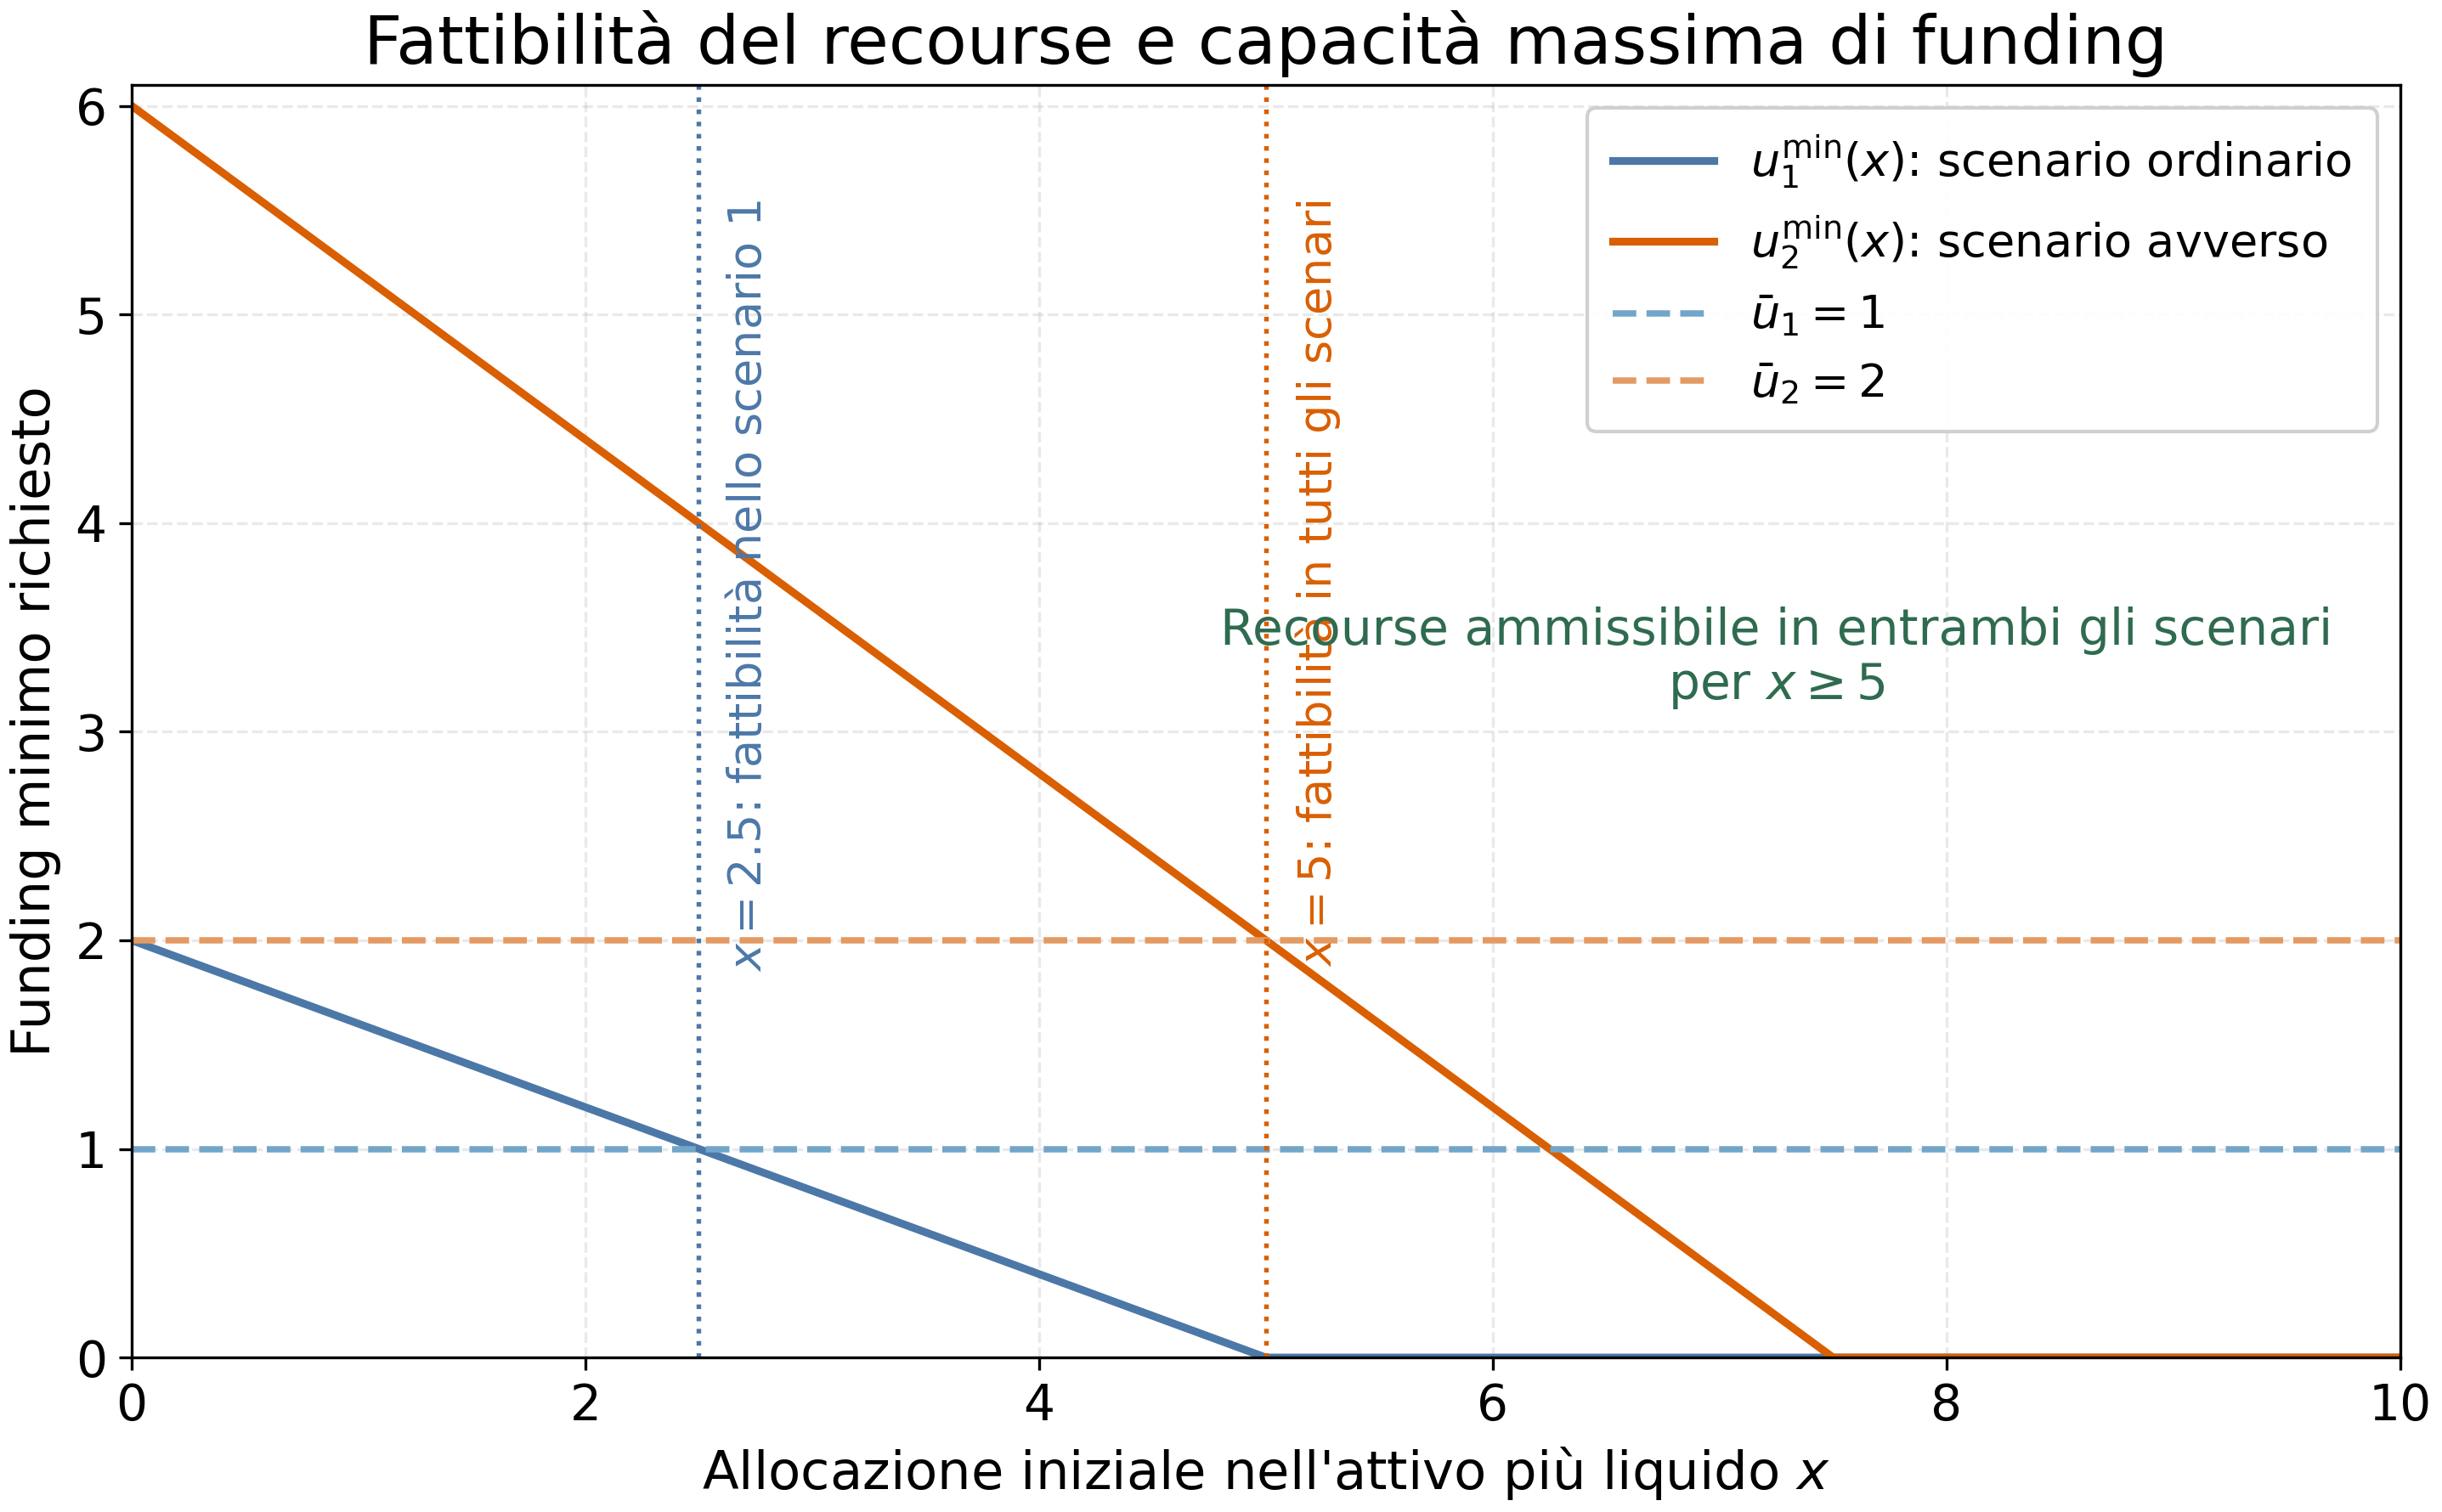
\includegraphics[width=0.94\textwidth]
{../graphics/Cap15_fattibilita_ricorso.png}
\caption{Funding minimo richiesto nei due scenari al variare
dell'allocazione iniziale nella classe di attivo pi\`u liquida.
L'intersezione tra $u_s^{\min}(x)$ e la corrispondente capacit\`a massima
$\bar u_s$ individua la soglia oltre la quale il ricorso diventa ammissibile
nello scenario. Per $x\geq5$ il problema di secondo stadio \`e ammissibile in
entrambi gli scenari.}
\label{fig:cap15-fattibilita-ricorso}
\end{figure}

La figura evidenzia tre regioni. Per

\[
0\leq x<2.5,
\]

la capacit\`a di funding non \`e sufficiente nemmeno nello scenario ordinario.
Per

\[
2.5\leq x<5,
\]

il ricorso \`e ammissibile nello scenario ordinario ma non nello scenario
avverso. Infine, per

\[
x\geq5,
\]

entrambi i problemi di secondo stadio risultano ammissibili.

L'esempio permette ora di distinguere chiaramente la fattibilit\`a del singolo
ricorso dalla propriet\`a di ricorso relativamente completo.

Se l'insieme ammissibile di primo stadio \`e

\[
\mathcal X=[0,10],
\]

il modello non possiede ricorso relativamente completo. Esistono infatti
decisioni ammissibili di primo stadio, come $x=4$, per le quali almeno uno
scenario genera un problema di secondo stadio non ammissibile.

Se invece ulteriori vincoli di primo stadio restringono l'insieme a

\[
\mathcal X=[5,10],
\]

allora, per ogni $x\in\mathcal X$ e per entrambi gli scenari considerati,
esiste almeno una decisione di secondo stadio ammissibile. Il problema
possiede quindi ricorso relativamente completo.

Ci\`o non implica ricorso completo. Le capacit\`a di funding restano infatti
limitate. Se il termine noto del bilancio di secondo stadio producesse un
deficit sufficientemente elevato, nessuna decisione $u_s\leq\bar u_s$ potrebbe
compensarlo. La struttura di ricorso non \`e quindi in grado di fronteggiare
un termine noto arbitrario.

Nel caso SVB--ALM completo lo stesso meccanismo opera attraverso pi\`u date,
pi\`u classi di attivo e pi\`u limiti di funding. Una composizione iniziale
pu\`o risultare ammissibile al primo stadio ma lasciare la banca incapace di
soddisfare uno dei successivi bilanci di liquidit\`a in uno scenario severo.

La fattibilit\`a costituisce quindi il primo filtro nella valutazione di una
decisione stocastica. Soltanto dopo avere verificato l'esistenza delle
decisioni di ricorso ha senso studiarne il valore economico. La sezione
successiva analizza precisamente come la funzione $Q_s(x)$ varia al variare
della decisione iniziale.
%% Capitoli/MQF_Cap_16_Python_Programmazione_Stocastica.tex

\chapter{Applicazioni Python di programmazione stocastica}

\section{Obiettivi della lezione}

Capitolo in preparazione.


%

%TCIMACRO{\QSubDoc{Include MQF_Cap_02_Variabili_Casuali}%
%{%2multibyte Version: 5.50.0.2960 CodePage: 65001
% MQF_Manuale_Master_SW55_Memoir.tex
% Master del manuale MQF costruito sullo shell SW5.5 "Memoir Class for Configurable Typesetting".
% Versione modulare: i capitoli scritti sono inclusi con \input.%
% POSIZIONE DEI FILE
% Questo master deve stare nella cartella 01_Manuale.
% I capitoli devono stare nella sottocartella 01_Manuale/Capitoli.
% Non mettere il master dentro Capitoli.
% I capitoli futuri restano come traccia, ma non generano pagine nel documento.
% Evita pagine bianche dovute all'apertura dei capitoli su pagina dispari.
% ------------------------------------------------------------
% Nomi italiani
% ------------------------------------------------------------
% ------------------------------------------------------------
% Macro matematiche ufficiali del progetto MQF
% Coerenti con MQF_Notazione.tex
% ------------------------------------------------------------
% ------------------------------------------------------------
% Ambienti di tipo teorema.
% I nomi interni restano compatibili con lo shell SW.
% Le etichette stampate sono in italiano.
% ------------------------------------------------------------

%TCIDATA{OutputFilter=latex2.dll}
%TCIDATA{Version=5.50.0.2960}
%TCIDATA{LaTeXparent=1,1,MQF_Manuale_Master.tex}


\chapter{Variabili casuali e distribuzioni}

\section{Obiettivi della lezione}

\label{sec:cap2-obiettivi}

Nel Capitolo 1 sono stati introdotti gli elementi fondamentali del linguaggio
probabilistico: lo spazio degli esiti, gli eventi, le operazioni sugli eventi
e la misura di probabilit\`{a}. Tale linguaggio consente di descrivere
l'incertezza in termini di eventi del tipo ``un certo scenario si verifica''
oppure ``un certo insieme di esiti si realizza''.

In molte applicazioni della finanza quantitativa, tuttavia, l'interesse
principale non \`{e} rivolto direttamente agli esiti elementari dello spazio
campionario, ma a quantit\`{a} numeriche che dipendono da tali esiti. Un
rendimento futuro, una perdita di portafoglio, il prezzo futuro di
un'attivit\`{a} finanziaria o il payoff di un contratto derivato sono esempi
di grandezze aleatorie. Formalmente, esse sono rappresentate mediante
variabili casuali, cio\`{e} funzioni del tipo
\[
X:\Omega\longrightarrow\mathbb{R}.
\]


Lo scopo di questo capitolo \`{e} introdurre il linguaggio delle variabili
casuali e delle loro distribuzioni. Il passaggio concettuale fondamentale
\`{e} il seguente: da una probabilit\`{a} definita sugli eventi dello spazio
campionario si costruisce una descrizione probabilistica dei valori assunti da
una grandezza numerica aleatoria. In questo modo diventa possibile studiare
eventi finanziariamente rilevanti quali
\[
\{R<0\},\qquad\{L>\ell\},\qquad\{S_{T}>K\},
\]
dove $R$ pu\`{o} rappresentare un rendimento, $L$ una perdita e $S_{T}$ il
prezzo futuro di un'attivit\`{a} finanziaria.

Al termine della lezione lo studente dovr\`{a} essere in grado di:

\begin{enumerate}
\item definire una variabile casuale come funzione misurabile dallo spazio
campionario alla retta reale;

\item interpretare eventi del tipo
\[
\{X\leq x\},\qquad\{X=x_{i}\},\qquad\{a<X\leq b\}
\]
come eventi appartenenti alla sigma-algebra $\mathcal{F}$;

\item definire la distribuzione di una variabile casuale e la funzione di
ripartizione
\[
F_{X}(x)=\mathbb{P}(X\leq x);
\]


\item distinguere tra variabili casuali discrete, descritte mediante una
funzione di massa $p_{X}$, e variabili casuali assolutamente continue,
descritte mediante una densit\`{a} $f_{X}$;

\item calcolare probabilit\`{a} associate a intervalli e code distributive,
usando la funzione di ripartizione, la funzione di massa o la densit\`{a};

\item definire e interpretare il valore atteso
\[
\mathbb{E}[X],
\]
la varianza
\[
\operatorname{Var}(X),
\]
la deviazione standard e, pi\`{u} in generale, i momenti di una variabile casuale;

\item calcolare il valore atteso di funzioni di variabili casuali, con
particolare riferimento a payoff finanziari del tipo $g(X)$;

\item introdurre il concetto di quantile, con particolare attenzione alla sua
interpretazione nella misura delle perdite e del rischio;

\item riconoscere alcune famiglie distributive fondamentali, tra cui le
distribuzioni di Bernoulli, binomiale, di Poisson, uniforme, normale e lognormale.
\end{enumerate}

Il capitolo costruisce quindi il ponte tra la teoria degli eventi e la
misurazione quantitativa del rischio. La sequenza logica che guider\`{a}
l'esposizione \`{e}
\[
(\Omega,\mathcal{F},\mathbb{P}) \quad\longrightarrow\quad X \quad
\longrightarrow\quad F_{X},\ p_{X},\ f_{X} \quad\longrightarrow\quad
\mathbb{E}[X],\ \operatorname{Var}(X),\ q_{\alpha}(X).
\]
Questa sequenza permette di passare dalla descrizione astratta dell'incertezza
alla rappresentazione analitica di rendimenti, perdite e payoff aleatori.

\section{Motivazione finanziaria: rendimenti, perdite e payoff aleatori}

\label{sec:cap2-motivazione-finanziaria}

Nelle applicazioni finanziarie l'incertezza non riguarda soltanto il
verificarsi o meno di un evento, ma soprattutto il valore numerico assunto da
una grandezza economica o finanziaria. L'esito futuro di un mercato pu\`{o}
determinare un rendimento positivo o negativo, una perdita di portafoglio, il
prezzo futuro di un'attivit\`{a} finanziaria o il payoff di un contratto
derivato. Tali grandezze non sono note al tempo iniziale, ma diventano note
solo dopo la realizzazione dello scenario rilevante.

Il linguaggio degli eventi, introdotto nel Capitolo 1, consente di formulare
affermazioni del tipo
\[
A=\{\text{il mercato scende}\}, \qquad B=\{\text{il debitore non rimborsa il
prestito}\}.
\]
Tuttavia, in molti problemi di finanza quantitativa, \`{e} necessario
descrivere non solo se un evento si verifica, ma anche quanto vale una
determinata grandezza in ciascuno scenario. Per questo motivo si introduce il
concetto di variabile casuale.

Ad esempio, se $R$ indica il rendimento aleatorio di un'attivit\`{a}
finanziaria, non interessa soltanto l'evento
\[
\{R<0\},
\]
cio\`{e} l'evento in cui il rendimento \`{e} negativo. Interessa anche la
distribuzione dei possibili valori di $R$, perch\'{e} tale distribuzione
consente di valutare la probabilit\`{a} di perdite moderate, di perdite
estreme, di rendimenti elevati o di risultati prossimi al valore medio.

In modo analogo, se $L$ indica la perdita aleatoria di un portafoglio, eventi
del tipo
\[
\{L>\ell\}
\]
descrivono il superamento di una soglia di perdita $\ell$. La quantit\`{a}
\[
\mathbb{P}(L>\ell)
\]
rappresenta quindi una probabilit\`{a} di coda, cio\`{e} la probabilit\`{a}
che la perdita superi un livello prefissato. Questo tipo di probabilit\`{a}
\`{e} centrale nella misurazione del rischio finanziario, poich\'{e} permette
di studiare non soltanto il comportamento medio di un portafoglio, ma anche la
severit\`{a} degli scenari sfavorevoli.

Un terzo esempio fondamentale \`{e} fornito dai contratti derivati. Sia
$S_{T}$ il prezzo aleatorio, al tempo futuro $T$, di un'attivit\`{a}
sottostante. Il payoff di un'opzione call europea con prezzo di esercizio $K$
\`{e}
\[
H=(S_{T}-K)^{+},
\]
dove
\[
(S_{T}-K)^{+}=\max\{S_{T}-K,0\}.
\]
Anche in questo caso il payoff $H$ \`{e} una variabile casuale: il suo valore
dipende dallo scenario futuro e, in particolare, dal valore assunto da $S_{T}%
$. L'evento
\[
\{S_{T}>K\}
\]
indica che l'opzione termina in the money, mentre la quantit\`{a}
\[
\mathbb{P}(S_{T}>K)
\]
misura la probabilit\`{a} che il payoff sia strettamente positivo.

Questi esempi mostrano che una parte rilevante della finanza quantitativa
pu\`{o} essere formulata mediante grandezze aleatorie numeriche:
\[%
\begin{array}
[c]{ll}%
R=\mbox{rendimento aleatorio}, & L=\mbox{perdita aleatoria},\\[4pt]%
S_{T}=\mbox{prezzo futuro aleatorio}, & H=\mbox{payoff aleatorio}.
\end{array}
\]
La variabile casuale \`{e} dunque lo strumento matematico che consente di
associare un numero reale a ciascuno scenario possibile.

Il problema centrale diventa allora descrivere la distribuzione probabilistica
di tali grandezze. In particolare, si vogliono rispondere domande del tipo:
\[
\mathbb{P}(R<0)=?
\]
\[
\mathbb{P}(L>\ell)=?
\]
\[
\mathbb{E}[R]=?
\]
\[
\operatorname{Var}(R)=?
\]
\[
q_{\alpha}(L)=?
\]
Le prime due domande riguardano probabilit\`{a} di eventi definiti tramite
variabili casuali. La terza riguarda il rendimento medio atteso. La quarta
riguarda la dispersione del rendimento intorno al proprio valore atteso. La
quinta riguarda un quantile della distribuzione della perdita, cio\`{e} una
soglia che viene superata solo con una probabilit\`{a} prefissata.

In questa prospettiva, una variabile casuale non \`{e} semplicemente un numero
incerto. Essa \`{e} una funzione che trasforma gli esiti elementari in valori
numerici:
\[
X:\Omega\longrightarrow\mathbb{R}.
\]
La probabilit\`{a}, definita originariamente sugli eventi dello spazio
campionario, induce cos\`{\i} una distribuzione sui valori assunti da $X$.
Questo passaggio \`{e} essenziale: permette di sostituire la descrizione
astratta degli scenari con una descrizione quantitativa dei risultati
economici associati a tali scenari.

Il capitolo sviluppa quindi gli strumenti necessari per descrivere e
utilizzare questa distribuzione: la funzione di ripartizione $F_{X}$, la
funzione di massa $p_{X}$ nel caso discreto, la densit\`{a} $f_{X}$ nel caso
continuo, il valore atteso, la varianza, i momenti e i quantili. Questi
oggetti costituiscono la base probabilistica per l'analisi di rendimenti,
perdite, payoff e rischio finanziario.

\section{Dallo spazio degli eventi alle variabili casuali}

\label{sec:cap2-dallo-spazio-eventi-vc}

Nel Capitolo 1 l'incertezza \`{e} stata descritta mediante uno spazio di
probabilit\`{a}
\[
(\Omega,\mathcal{F},\mathbb{P}),
\]
dove $\Omega$ rappresenta l'insieme degli esiti possibili, $\mathcal{F}$ \`{e}
la sigma-algebra degli eventi osservabili e $\mathbb{P}$ \`{e} la misura di
probabilit\`{a} definita su tali eventi.

In molte applicazioni, tuttavia, non interessa direttamente l'esito elementare
$\omega\in\Omega$, ma una quantit\`{a} numerica che dipende da tale esito. Una
variabile casuale formalizza precisamente questo passaggio.

\begin{definition}
[Variabile casuale]Sia $(\Omega,\mathcal{F},\mathbb{P})$ uno spazio di
probabilit\`{a}. Una variabile casuale reale \`{e} una funzione
\[
X:\Omega\longrightarrow\mathbb{R}
\]
tale che, per ogni $x\in\mathbb{R}$,
\[
\{\omega\in\Omega:X(\omega)\leq x\}\in\mathcal{F}.
\]

\end{definition}

La condizione precedente significa che, per ogni soglia reale $x$, l'insieme
degli esiti per i quali la variabile casuale assume un valore non superiore a
$x$ \`{e} un evento. Di conseguenza, la sua probabilit\`{a} \`{e} ben definita.

Per alleggerire la notazione, si scrive normalmente
\[
\{X\leq x\}
\]
al posto di
\[
\{\omega\in\Omega:X(\omega)\leq x\}.
\]
Con questa convenzione, la quantit\`{a}
\[
\mathbb{P}(X\leq x)
\]
deve essere letta come abbreviazione di
\[
\mathbb{P}(\{\omega\in\Omega:X(\omega)\leq x\}).
\]


In modo analogo, scritture come
\[
\{X=x_{i}\},\qquad\{a<X\leq b\},\qquad\{X\in B\}
\]
indicano rispettivamente gli eventi
\[
\{\omega\in\Omega:X(\omega)=x_{i}\},
\]
\[
\{\omega\in\Omega:a<X(\omega)\leq b\},
\]
\[
\{\omega\in\Omega:X(\omega)\in B\},
\]
dove $B$ \`{e} un sottoinsieme opportuno della retta reale.

\paragraph{Esempio guida: rendimento discreto su tre regimi di mercato.}

Consideriamo un modello elementare con sei esiti possibili:
\[
\Omega=\{\omega_{1},\omega_{2},\omega_{3},\omega_{4},\omega_{5},\omega_{6}\}.
\]
Gli esiti elementari rappresentano sei scenari di mercato. Supponiamo tuttavia
che l'informazione rilevante distingua soltanto tre regimi: mercato
sfavorevole, mercato intermedio e mercato favorevole. Introduciamo quindi la
partizione
\[
A_{1}=\{\omega_{1},\omega_{2}\}, \qquad A_{2}=\{\omega_{3},\omega_{4}\},
\qquad A_{3}=\{\omega_{5},\omega_{6}\}.
\]
L'evento $A_{1}$ rappresenta il regime sfavorevole, $A_{2}$ il regime
intermedio e $A_{3}$ il regime favorevole. La sigma-algebra generata da questa
partizione \`{e}
\[
\mathcal{F}=\sigma(A_{1},A_{2},A_{3}).
\]
Esplicitamente,
\[
\mathcal{F}= \{\varnothing, A_{1},A_{2},A_{3}, A_{1}\cup A_{2},A_{1}\cup
A_{3},A_{2}\cup A_{3}, \Omega\}.
\]
In questo modello non tutte le distinzioni tra gli esiti elementari sono
osservabili attraverso $\mathcal{F}$: gli eventi ammissibili sono le unioni
degli elementi della partizione.

Definiamo ora una variabile casuale $X$ che rappresenta il rendimento di un
portafoglio in ciascuno scenario. Supponiamo che il rendimento dipenda
soltanto dal regime di mercato e sia dato dalla seguente tabella:
\[%
\begin{array}
[c]{c|c|c}%
\mbox{esito} & \mbox{regime} & X(\omega)\\\hline
\omega_{1},\omega_{2} & A_{1}\ \mbox{sfavorevole} & -0.04\\
\omega_{3},\omega_{4} & A_{2}\ \mbox{intermedio} & 0.01\\
\omega_{5},\omega_{6} & A_{3}\ \mbox{favorevole} & 0.06
\end{array}
\]
La variabile casuale $X$ trasforma quindi i sei esiti elementari in tre valori
reali:
\[
x_{1}=-0.04, \qquad x_{2}=0.01, \qquad x_{3}=0.06.
\]
I tre valori assunti da $X$ determinano una partizione sulla retta reale. Le
regioni rilevanti sono
\[
(-\infty,-0.04), \qquad[-0.04,0.01), \qquad[0.01,0.06, \qquad[0.06,+\infty).
\]
Eventi descritti in termini di rendimenti (valori numerici) $X \in\mathbb{R}$
sono in corrispondenza con eventi qualitativi in $\Omega$. Ad esempio,
l'evento ``rendimento negativo'' \`{e}
\[
\{X<0\}=A_{1}=\{\omega_{1},\omega_{2}\}.
\]
L'evento ``rendimento almeno pari all'$1\%$'' \`{e}
\[
\{X\geq0.01\}=A_{2}\cup A_{3} =\{\omega_{3},\omega_{4},\omega_{5},\omega
_{6}\}.
\]
L'evento ``rendimento non superiore all'$1\%$'' \`{e}
\[
\{X\leq0.01\}=A_{1}\cup A_{2} =\{\omega_{1},\omega_{2},\omega_{3},\omega
_{4}\}.
\]
In tutti questi casi la probabilit\`{a} resta formalmente una probabilit\`{a}
assegnata a eventi appartenenti a $\mathcal{F}$:
\[
\mathbb{P}(X<0)=\mathbb{P}(A_{1}),
\]
\[
\mathbb{P}(X\geq0.01)=\mathbb{P}(A_{2}\cup A_{3}),
\]
\[
\mathbb{P}(X\leq0.01)=\mathbb{P}(A_{1}\cup A_{2}).
\]
La variabile casuale consente per\`{o} di descrivere tali eventi mediante
condizioni sui valori numerici del rendimento.

\paragraph{Controimmagini e misurabilit\`{a}.}

Il legame formale tra valori numerici ed eventi \`{e} dato dalla nozione di
controimmagine. Sia
\[
X:\Omega\longrightarrow\mathbb{R}
\]
una funzione e sia $B\subseteq\mathbb{R}$. Si definisce controimmagine di $B$
mediante $X$ l'insieme
\[
X^{-1}(B)=\{\omega\in\Omega:X(\omega)\in B\}.
\]
La controimmagine $X^{-1}(B)$ \`{e} quindi un sottoinsieme di $\Omega$: essa
raccoglie tutti gli esiti elementari che, attraverso la funzione $X$, vengono
mandati in $B$.

La notazione $X^{-1}(B)$ indica l'insieme degli esiti la cui immagine
appartiene a $B$. Ad esempio, se $B=(-\infty,a]$, allora
\[
X^{-1}((-\infty,a]) = \{\omega\in\Omega:X(\omega)\leq a\} = \{X\leq a\}.
\]
Analogamente,
\[
X^{-1}((a,b]) = \{\omega\in\Omega:a<X(\omega)\leq b\} = \{a<X\leq b\}.
\]


La nozione di variabile casuale richiede che queste controimmagini siano
eventi ai quali sia possibile assegnare una probabilit\`{a}. Per garantire
questo fatto si dimostra che \`{e} necessario e sufficiente che, per ogni
scelta arbitraria del valore $a\in\mathbf{R}$ negli intervalli di tipo
$(-\infty,a],$ risulti:%
\begin{equation}
X^{-1}(-\infty,a]\in\mathcal{F}.\label{cmisur}%
\end{equation}
Se vale la precedente condizione, allora discende anche
\[
X^{-1}(a,b]\in\mathcal{F}%
\]
per ogni scelta di $a,b$.  In termini generali, una funzione $X:\Omega
\rightarrow\mathbb{R}$ per cui vale la condizione \ref{cmisur} \`{e} detta
variabile casuale \textbf{misurabile}.

Nel seguito useremo prevalentemente eventi del tipo
\[
\{X\leq x\},\qquad\{a<X\leq b\},\qquad\{X\in B\},
\]
poich\'{e} sono quelli che permettono di costruire la funzione di
ripartizione, la funzione di massa, la densit\`{a} e i quantili.

\begin{example}
[Controimmagini nell'esempio del rendimento discreto]Riprendiamo la variabile
casuale $X$ definita sull'insieme
\[
\Omega=\{\omega_{1},\omega_{2},\omega_{3},\omega_{4},\omega_{5},\omega_{6}\}
\]
mediante la tabella
\[%
\begin{array}
[c]{c|c|c}%
\mbox{esito} & \mbox{regime} & X(\omega)\\\hline
\omega_{1},\omega_{2} & A_{1}\ \mbox{sfavorevole} & -0.04\\
\omega_{3},\omega_{4} & A_{2}\ \mbox{intermedio} & 0.01\\
\omega_{5},\omega_{6} & A_{3}\ \mbox{favorevole} & 0.06
\end{array}
\]
dove
\[
A_{1}=\{\omega_{1},\omega_{2}\}, \qquad A_{2}=\{\omega_{3},\omega_{4}\},
\qquad A_{3}=\{\omega_{5},\omega_{6}\}.
\]
La sigma-algebra considerata \`{e}
\[
\mathcal{F}=\sigma(A_{1},A_{2},A_{3}) = \{\varnothing, A_{1},A_{2},A_{3},
A_{1}\cup A_{2},A_{1}\cup A_{3},A_{2}\cup A_{3}, \Omega\}.
\]


Poich\'{e} i possibili rendimenti $X$ assumo soltanto i valori%
\[
-0.04<0.01<0.06,
\]
la controimmagine di un intervallo del tipo $(-\infty,a]$ dipende dalla
posizione della soglia $a$ rispetto a questi tre valori. Si ottiene:
\[%
\begin{array}
[c]{c|c}%
\text{valori }a\text{ per intervalli }(-\infty,a] & X^{-1}((-\infty
,a])=\{X\leq a\}\\\hline
a<-0.04 & \varnothing\\
-0.04\leq a<0.01 & A_{1}\\
0.01\leq a<0.06 & A_{1}\cup A_{2}\\
a\geq0.06 & \Omega
\end{array}
\]
Ogni insieme nella seconda colonna appartiene a $\mathcal{F}$. La tabella
mostra quindi, in modo esplicito, che $X$ \`{e} misurabile rispetto alla
sigma-algebra considerata.

La stessa logica vale per altri sottoinsiemi della retta reale. Ad esempio,
\[
X^{-1}([0,+\infty))=A_{2}\cup A_{3},
\]
perch\'{e} i valori non negativi di $X$ sono $0.01$ e $0.06$. Inoltre,
\[
X^{-1}((-\infty,0))=A_{1}.
\]
In termini finanziari, il primo evento rappresenta gli scenari con rendimento
non negativo, mentre il secondo rappresenta gli scenari con rendimento negativo.
\end{example}

\paragraph{Variabili indicatrici.}

Un caso particolarmente importante di variabile casuale \`{e} la variabile
indicatrice di un evento. Se $A\in\mathcal{F}$, si definisce
\[
\mathbf{1}_{A}(\omega)=
\begin{cases}
1, & \mbox{se }\omega\in A,\\
0, & \mbox{se }\omega\notin A.
\end{cases}
\]
La variabile $\mathbf{1}_{A}$ assume quindi valore $1$ quando l'evento $A$ si
verifica e valore $0$ quando l'evento non si verifica.

Nell'esempio del rendimento discreto, l'indicatrice dell'evento di rendimento
negativo \`{e}
\[
\mathbf{1}_{\{X<0\}}=\mathbf{1}_{A_{1}}.
\]
Essa vale $1$ negli scenari $\omega_{1}$ e $\omega_{2}$, e vale $0$ negli
altri scenari. Analogamente, l'indicatrice dell'evento di rendimento almeno
pari all'$1\%$ \`{e}
\[
\mathbf{1}_{\{X\geq0.01\}}=\mathbf{1}_{A_{2}\cup A_{3}}.
\]


Nelle applicazioni finanziarie, variabili indicatrici di questo tipo compaiono
frequentemente:
\[
\mathbf{1}_{\{R<0\}}, \qquad\mathbf{1}_{\{L>\ell\}}, \qquad\mathbf{1}%
_{\{S_{T}>K\}}.
\]
Esse indicano rispettivamente il verificarsi di un rendimento negativo, il
superamento di una soglia di perdita e il superamento dello strike da parte
del sottostante. Saranno utili anche per rappresentare payoff digitali, eventi
di default e vincoli probabilistici.

In conclusione, una variabile casuale non sostituisce lo spazio di
probabilit\`{a}, ma lo utilizza per costruire una descrizione numerica
dell'incertezza. Lo spazio $(\Omega,\mathcal{F},\mathbb{P})$ resta il
fondamento formale; la variabile casuale $X$ traduce gli esiti $\omega$ in
valori reali $X(\omega)$; la distribuzione di $X$, introdotta nella sezione
successiva, descrive la probabilit\`{a} con cui tali valori possono manifestarsi.}}%
%BeginExpansion
%2multibyte Version: 5.50.0.2960 CodePage: 65001
% MQF_Manuale_Master_SW55_Memoir.tex
% Master del manuale MQF costruito sullo shell SW5.5 "Memoir Class for Configurable Typesetting".
% Versione modulare: i capitoli scritti sono inclusi con \input.%
% POSIZIONE DEI FILE
% Questo master deve stare nella cartella 01_Manuale.
% I capitoli devono stare nella sottocartella 01_Manuale/Capitoli.
% Non mettere il master dentro Capitoli.
% I capitoli futuri restano come traccia, ma non generano pagine nel documento.
% Evita pagine bianche dovute all'apertura dei capitoli su pagina dispari.
% ------------------------------------------------------------
% Nomi italiani
% ------------------------------------------------------------
% ------------------------------------------------------------
% Macro matematiche ufficiali del progetto MQF
% Coerenti con MQF_Notazione.tex
% ------------------------------------------------------------
% ------------------------------------------------------------
% Ambienti di tipo teorema.
% I nomi interni restano compatibili con lo shell SW.
% Le etichette stampate sono in italiano.
% ------------------------------------------------------------

%TCIDATA{OutputFilter=latex2.dll}
%TCIDATA{Version=5.50.0.2960}
%TCIDATA{LaTeXparent=1,1,MQF_Manuale_Master.tex}


\chapter{Variabili casuali e distribuzioni}

\section{Obiettivi della lezione}

\label{sec:cap2-obiettivi}

Nel Capitolo 1 sono stati introdotti gli elementi fondamentali del linguaggio
probabilistico: lo spazio degli esiti, gli eventi, le operazioni sugli eventi
e la misura di probabilit\`{a}. Tale linguaggio consente di descrivere
l'incertezza in termini di eventi del tipo ``un certo scenario si verifica''
oppure ``un certo insieme di esiti si realizza''.

In molte applicazioni della finanza quantitativa, tuttavia, l'interesse
principale non \`{e} rivolto direttamente agli esiti elementari dello spazio
campionario, ma a quantit\`{a} numeriche che dipendono da tali esiti. Un
rendimento futuro, una perdita di portafoglio, il prezzo futuro di
un'attivit\`{a} finanziaria o il payoff di un contratto derivato sono esempi
di grandezze aleatorie. Formalmente, esse sono rappresentate mediante
variabili casuali, cio\`{e} funzioni del tipo
\[
X:\Omega\longrightarrow\mathbb{R}.
\]


Lo scopo di questo capitolo \`{e} introdurre il linguaggio delle variabili
casuali e delle loro distribuzioni. Il passaggio concettuale fondamentale
\`{e} il seguente: da una probabilit\`{a} definita sugli eventi dello spazio
campionario si costruisce una descrizione probabilistica dei valori assunti da
una grandezza numerica aleatoria. In questo modo diventa possibile studiare
eventi finanziariamente rilevanti quali
\[
\{R<0\},\qquad\{L>\ell\},\qquad\{S_{T}>K\},
\]
dove $R$ pu\`{o} rappresentare un rendimento, $L$ una perdita e $S_{T}$ il
prezzo futuro di un'attivit\`{a} finanziaria.

Al termine della lezione lo studente dovr\`{a} essere in grado di:

\begin{enumerate}
\item definire una variabile casuale come funzione misurabile dallo spazio
campionario alla retta reale;

\item interpretare eventi del tipo
\[
\{X\leq x\},\qquad\{X=x_{i}\},\qquad\{a<X\leq b\}
\]
come eventi appartenenti alla sigma-algebra $\mathcal{F}$;

\item definire la distribuzione di una variabile casuale e la funzione di
ripartizione
\[
F_{X}(x)=\mathbb{P}(X\leq x);
\]


\item distinguere tra variabili casuali discrete, descritte mediante una
funzione di massa $p_{X}$, e variabili casuali assolutamente continue,
descritte mediante una densit\`{a} $f_{X}$;

\item calcolare probabilit\`{a} associate a intervalli e code distributive,
usando la funzione di ripartizione, la funzione di massa o la densit\`{a};

\item definire e interpretare il valore atteso
\[
\mathbb{E}[X],
\]
la varianza
\[
\operatorname{Var}(X),
\]
la deviazione standard e, pi\`{u} in generale, i momenti di una variabile casuale;

\item calcolare il valore atteso di funzioni di variabili casuali, con
particolare riferimento a payoff finanziari del tipo $g(X)$;

\item introdurre il concetto di quantile, con particolare attenzione alla sua
interpretazione nella misura delle perdite e del rischio;

\item riconoscere alcune famiglie distributive fondamentali, tra cui le
distribuzioni di Bernoulli, binomiale, di Poisson, uniforme, normale e lognormale.
\end{enumerate}

Il capitolo costruisce quindi il ponte tra la teoria degli eventi e la
misurazione quantitativa del rischio. La sequenza logica che guider\`{a}
l'esposizione \`{e}
\[
(\Omega,\mathcal{F},\mathbb{P}) \quad\longrightarrow\quad X \quad
\longrightarrow\quad F_{X},\ p_{X},\ f_{X} \quad\longrightarrow\quad
\mathbb{E}[X],\ \operatorname{Var}(X),\ q_{\alpha}(X).
\]
Questa sequenza permette di passare dalla descrizione astratta dell'incertezza
alla rappresentazione analitica di rendimenti, perdite e payoff aleatori.

\section{Motivazione finanziaria: rendimenti, perdite e payoff aleatori}

\label{sec:cap2-motivazione-finanziaria}

Nelle applicazioni finanziarie l'incertezza non riguarda soltanto il
verificarsi o meno di un evento, ma soprattutto il valore numerico assunto da
una grandezza economica o finanziaria. L'esito futuro di un mercato pu\`{o}
determinare un rendimento positivo o negativo, una perdita di portafoglio, il
prezzo futuro di un'attivit\`{a} finanziaria o il payoff di un contratto
derivato. Tali grandezze non sono note al tempo iniziale, ma diventano note
solo dopo la realizzazione dello scenario rilevante.

Il linguaggio degli eventi, introdotto nel Capitolo 1, consente di formulare
affermazioni del tipo
\[
A=\{\text{il mercato scende}\}, \qquad B=\{\text{il debitore non rimborsa il
prestito}\}.
\]
Tuttavia, in molti problemi di finanza quantitativa, \`{e} necessario
descrivere non solo se un evento si verifica, ma anche quanto vale una
determinata grandezza in ciascuno scenario. Per questo motivo si introduce il
concetto di variabile casuale.

Ad esempio, se $R$ indica il rendimento aleatorio di un'attivit\`{a}
finanziaria, non interessa soltanto l'evento
\[
\{R<0\},
\]
cio\`{e} l'evento in cui il rendimento \`{e} negativo. Interessa anche la
distribuzione dei possibili valori di $R$, perch\'{e} tale distribuzione
consente di valutare la probabilit\`{a} di perdite moderate, di perdite
estreme, di rendimenti elevati o di risultati prossimi al valore medio.

In modo analogo, se $L$ indica la perdita aleatoria di un portafoglio, eventi
del tipo
\[
\{L>\ell\}
\]
descrivono il superamento di una soglia di perdita $\ell$. La quantit\`{a}
\[
\mathbb{P}(L>\ell)
\]
rappresenta quindi una probabilit\`{a} di coda, cio\`{e} la probabilit\`{a}
che la perdita superi un livello prefissato. Questo tipo di probabilit\`{a}
\`{e} centrale nella misurazione del rischio finanziario, poich\'{e} permette
di studiare non soltanto il comportamento medio di un portafoglio, ma anche la
severit\`{a} degli scenari sfavorevoli.

Un terzo esempio fondamentale \`{e} fornito dai contratti derivati. Sia
$S_{T}$ il prezzo aleatorio, al tempo futuro $T$, di un'attivit\`{a}
sottostante. Il payoff di un'opzione call europea con prezzo di esercizio $K$
\`{e}
\[
H=(S_{T}-K)^{+},
\]
dove
\[
(S_{T}-K)^{+}=\max\{S_{T}-K,0\}.
\]
Anche in questo caso il payoff $H$ \`{e} una variabile casuale: il suo valore
dipende dallo scenario futuro e, in particolare, dal valore assunto da $S_{T}%
$. L'evento
\[
\{S_{T}>K\}
\]
indica che l'opzione termina in the money, mentre la quantit\`{a}
\[
\mathbb{P}(S_{T}>K)
\]
misura la probabilit\`{a} che il payoff sia strettamente positivo.

Questi esempi mostrano che una parte rilevante della finanza quantitativa
pu\`{o} essere formulata mediante grandezze aleatorie numeriche:
\[%
\begin{array}
[c]{ll}%
R=\mbox{rendimento aleatorio}, & L=\mbox{perdita aleatoria},\\[4pt]%
S_{T}=\mbox{prezzo futuro aleatorio}, & H=\mbox{payoff aleatorio}.
\end{array}
\]
La variabile casuale \`{e} dunque lo strumento matematico che consente di
associare un numero reale a ciascuno scenario possibile.

Il problema centrale diventa allora descrivere la distribuzione probabilistica
di tali grandezze. In particolare, si vogliono rispondere domande del tipo:
\[
\mathbb{P}(R<0)=?
\]
\[
\mathbb{P}(L>\ell)=?
\]
\[
\mathbb{E}[R]=?
\]
\[
\operatorname{Var}(R)=?
\]
\[
q_{\alpha}(L)=?
\]
Le prime due domande riguardano probabilit\`{a} di eventi definiti tramite
variabili casuali. La terza riguarda il rendimento medio atteso. La quarta
riguarda la dispersione del rendimento intorno al proprio valore atteso. La
quinta riguarda un quantile della distribuzione della perdita, cio\`{e} una
soglia che viene superata solo con una probabilit\`{a} prefissata.

In questa prospettiva, una variabile casuale non \`{e} semplicemente un numero
incerto. Essa \`{e} una funzione che trasforma gli esiti elementari in valori
numerici:
\[
X:\Omega\longrightarrow\mathbb{R}.
\]
La probabilit\`{a}, definita originariamente sugli eventi dello spazio
campionario, induce cos\`{\i} una distribuzione sui valori assunti da $X$.
Questo passaggio \`{e} essenziale: permette di sostituire la descrizione
astratta degli scenari con una descrizione quantitativa dei risultati
economici associati a tali scenari.

Il capitolo sviluppa quindi gli strumenti necessari per descrivere e
utilizzare questa distribuzione: la funzione di ripartizione $F_{X}$, la
funzione di massa $p_{X}$ nel caso discreto, la densit\`{a} $f_{X}$ nel caso
continuo, il valore atteso, la varianza, i momenti e i quantili. Questi
oggetti costituiscono la base probabilistica per l'analisi di rendimenti,
perdite, payoff e rischio finanziario.

\section{Dallo spazio degli eventi alle variabili casuali}

\label{sec:cap2-dallo-spazio-eventi-vc}

Nel Capitolo 1 l'incertezza \`{e} stata descritta mediante uno spazio di
probabilit\`{a}
\[
(\Omega,\mathcal{F},\mathbb{P}),
\]
dove $\Omega$ rappresenta l'insieme degli esiti possibili, $\mathcal{F}$ \`{e}
la sigma-algebra degli eventi osservabili e $\mathbb{P}$ \`{e} la misura di
probabilit\`{a} definita su tali eventi.

In molte applicazioni, tuttavia, non interessa direttamente l'esito elementare
$\omega\in\Omega$, ma una quantit\`{a} numerica che dipende da tale esito. Una
variabile casuale formalizza precisamente questo passaggio.

\begin{definition}
[Variabile casuale]Sia $(\Omega,\mathcal{F},\mathbb{P})$ uno spazio di
probabilit\`{a}. Una variabile casuale reale \`{e} una funzione
\[
X:\Omega\longrightarrow\mathbb{R}
\]
tale che, per ogni $x\in\mathbb{R}$,
\[
\{\omega\in\Omega:X(\omega)\leq x\}\in\mathcal{F}.
\]

\end{definition}

La condizione precedente significa che, per ogni soglia reale $x$, l'insieme
degli esiti per i quali la variabile casuale assume un valore non superiore a
$x$ \`{e} un evento. Di conseguenza, la sua probabilit\`{a} \`{e} ben definita.

Per alleggerire la notazione, si scrive normalmente
\[
\{X\leq x\}
\]
al posto di
\[
\{\omega\in\Omega:X(\omega)\leq x\}.
\]
Con questa convenzione, la quantit\`{a}
\[
\mathbb{P}(X\leq x)
\]
deve essere letta come abbreviazione di
\[
\mathbb{P}(\{\omega\in\Omega:X(\omega)\leq x\}).
\]


In modo analogo, scritture come
\[
\{X=x_{i}\},\qquad\{a<X\leq b\},\qquad\{X\in B\}
\]
indicano rispettivamente gli eventi
\[
\{\omega\in\Omega:X(\omega)=x_{i}\},
\]
\[
\{\omega\in\Omega:a<X(\omega)\leq b\},
\]
\[
\{\omega\in\Omega:X(\omega)\in B\},
\]
dove $B$ \`{e} un sottoinsieme opportuno della retta reale.

\paragraph{Esempio guida: rendimento discreto su tre regimi di mercato.}

Consideriamo un modello elementare con sei esiti possibili:
\[
\Omega=\{\omega_{1},\omega_{2},\omega_{3},\omega_{4},\omega_{5},\omega_{6}\}.
\]
Gli esiti elementari rappresentano sei scenari di mercato. Supponiamo tuttavia
che l'informazione rilevante distingua soltanto tre regimi: mercato
sfavorevole, mercato intermedio e mercato favorevole. Introduciamo quindi la
partizione
\[
A_{1}=\{\omega_{1},\omega_{2}\}, \qquad A_{2}=\{\omega_{3},\omega_{4}\},
\qquad A_{3}=\{\omega_{5},\omega_{6}\}.
\]
L'evento $A_{1}$ rappresenta il regime sfavorevole, $A_{2}$ il regime
intermedio e $A_{3}$ il regime favorevole. La sigma-algebra generata da questa
partizione \`{e}
\[
\mathcal{F}=\sigma(A_{1},A_{2},A_{3}).
\]
Esplicitamente,
\[
\mathcal{F}= \{\varnothing, A_{1},A_{2},A_{3}, A_{1}\cup A_{2},A_{1}\cup
A_{3},A_{2}\cup A_{3}, \Omega\}.
\]
In questo modello non tutte le distinzioni tra gli esiti elementari sono
osservabili attraverso $\mathcal{F}$: gli eventi ammissibili sono le unioni
degli elementi della partizione.

Definiamo ora una variabile casuale $X$ che rappresenta il rendimento di un
portafoglio in ciascuno scenario. Supponiamo che il rendimento dipenda
soltanto dal regime di mercato e sia dato dalla seguente tabella:
\[%
\begin{array}
[c]{c|c|c}%
\mbox{esito} & \mbox{regime} & X(\omega)\\\hline
\omega_{1},\omega_{2} & A_{1}\ \mbox{sfavorevole} & -0.04\\
\omega_{3},\omega_{4} & A_{2}\ \mbox{intermedio} & 0.01\\
\omega_{5},\omega_{6} & A_{3}\ \mbox{favorevole} & 0.06
\end{array}
\]
La variabile casuale $X$ trasforma quindi i sei esiti elementari in tre valori
reali:
\[
x_{1}=-0.04, \qquad x_{2}=0.01, \qquad x_{3}=0.06.
\]
I tre valori assunti da $X$ determinano una partizione sulla retta reale. Le
regioni rilevanti sono
\[
(-\infty,-0.04), \qquad[-0.04,0.01), \qquad[0.01,0.06, \qquad[0.06,+\infty).
\]
Eventi descritti in termini di rendimenti (valori numerici) $X \in\mathbb{R}$
sono in corrispondenza con eventi qualitativi in $\Omega$. Ad esempio,
l'evento ``rendimento negativo'' \`{e}
\[
\{X<0\}=A_{1}=\{\omega_{1},\omega_{2}\}.
\]
L'evento ``rendimento almeno pari all'$1\%$'' \`{e}
\[
\{X\geq0.01\}=A_{2}\cup A_{3} =\{\omega_{3},\omega_{4},\omega_{5},\omega
_{6}\}.
\]
L'evento ``rendimento non superiore all'$1\%$'' \`{e}
\[
\{X\leq0.01\}=A_{1}\cup A_{2} =\{\omega_{1},\omega_{2},\omega_{3},\omega
_{4}\}.
\]
In tutti questi casi la probabilit\`{a} resta formalmente una probabilit\`{a}
assegnata a eventi appartenenti a $\mathcal{F}$:
\[
\mathbb{P}(X<0)=\mathbb{P}(A_{1}),
\]
\[
\mathbb{P}(X\geq0.01)=\mathbb{P}(A_{2}\cup A_{3}),
\]
\[
\mathbb{P}(X\leq0.01)=\mathbb{P}(A_{1}\cup A_{2}).
\]
La variabile casuale consente per\`{o} di descrivere tali eventi mediante
condizioni sui valori numerici del rendimento.

\paragraph{Controimmagini e misurabilit\`{a}.}

Il legame formale tra valori numerici ed eventi \`{e} dato dalla nozione di
controimmagine. Sia
\[
X:\Omega\longrightarrow\mathbb{R}
\]
una funzione e sia $B\subseteq\mathbb{R}$. Si definisce controimmagine di $B$
mediante $X$ l'insieme
\[
X^{-1}(B)=\{\omega\in\Omega:X(\omega)\in B\}.
\]
La controimmagine $X^{-1}(B)$ \`{e} quindi un sottoinsieme di $\Omega$: essa
raccoglie tutti gli esiti elementari che, attraverso la funzione $X$, vengono
mandati in $B$.

La notazione $X^{-1}(B)$ indica l'insieme degli esiti la cui immagine
appartiene a $B$. Ad esempio, se $B=(-\infty,a]$, allora
\[
X^{-1}((-\infty,a]) = \{\omega\in\Omega:X(\omega)\leq a\} = \{X\leq a\}.
\]
Analogamente,
\[
X^{-1}((a,b]) = \{\omega\in\Omega:a<X(\omega)\leq b\} = \{a<X\leq b\}.
\]


La nozione di variabile casuale richiede che queste controimmagini siano
eventi ai quali sia possibile assegnare una probabilit\`{a}. Per garantire
questo fatto si dimostra che \`{e} necessario e sufficiente che, per ogni
scelta arbitraria del valore $a\in\mathbf{R}$ negli intervalli di tipo
$(-\infty,a],$ risulti:%
\begin{equation}
X^{-1}(-\infty,a]\in\mathcal{F}.\label{cmisur}%
\end{equation}
Se vale la precedente condizione, allora discende anche
\[
X^{-1}(a,b]\in\mathcal{F}%
\]
per ogni scelta di $a,b$.  In termini generali, una funzione $X:\Omega
\rightarrow\mathbb{R}$ per cui vale la condizione \ref{cmisur} \`{e} detta
variabile casuale \textbf{misurabile}.

Nel seguito useremo prevalentemente eventi del tipo
\[
\{X\leq x\},\qquad\{a<X\leq b\},\qquad\{X\in B\},
\]
poich\'{e} sono quelli che permettono di costruire la funzione di
ripartizione, la funzione di massa, la densit\`{a} e i quantili.

\begin{example}
[Controimmagini nell'esempio del rendimento discreto]Riprendiamo la variabile
casuale $X$ definita sull'insieme
\[
\Omega=\{\omega_{1},\omega_{2},\omega_{3},\omega_{4},\omega_{5},\omega_{6}\}
\]
mediante la tabella
\[%
\begin{array}
[c]{c|c|c}%
\mbox{esito} & \mbox{regime} & X(\omega)\\\hline
\omega_{1},\omega_{2} & A_{1}\ \mbox{sfavorevole} & -0.04\\
\omega_{3},\omega_{4} & A_{2}\ \mbox{intermedio} & 0.01\\
\omega_{5},\omega_{6} & A_{3}\ \mbox{favorevole} & 0.06
\end{array}
\]
dove
\[
A_{1}=\{\omega_{1},\omega_{2}\}, \qquad A_{2}=\{\omega_{3},\omega_{4}\},
\qquad A_{3}=\{\omega_{5},\omega_{6}\}.
\]
La sigma-algebra considerata \`{e}
\[
\mathcal{F}=\sigma(A_{1},A_{2},A_{3}) = \{\varnothing, A_{1},A_{2},A_{3},
A_{1}\cup A_{2},A_{1}\cup A_{3},A_{2}\cup A_{3}, \Omega\}.
\]


Poich\'{e} i possibili rendimenti $X$ assumo soltanto i valori%
\[
-0.04<0.01<0.06,
\]
la controimmagine di un intervallo del tipo $(-\infty,a]$ dipende dalla
posizione della soglia $a$ rispetto a questi tre valori. Si ottiene:
\[%
\begin{array}
[c]{c|c}%
\text{valori }a\text{ per intervalli }(-\infty,a] & X^{-1}((-\infty
,a])=\{X\leq a\}\\\hline
a<-0.04 & \varnothing\\
-0.04\leq a<0.01 & A_{1}\\
0.01\leq a<0.06 & A_{1}\cup A_{2}\\
a\geq0.06 & \Omega
\end{array}
\]
Ogni insieme nella seconda colonna appartiene a $\mathcal{F}$. La tabella
mostra quindi, in modo esplicito, che $X$ \`{e} misurabile rispetto alla
sigma-algebra considerata.

La stessa logica vale per altri sottoinsiemi della retta reale. Ad esempio,
\[
X^{-1}([0,+\infty))=A_{2}\cup A_{3},
\]
perch\'{e} i valori non negativi di $X$ sono $0.01$ e $0.06$. Inoltre,
\[
X^{-1}((-\infty,0))=A_{1}.
\]
In termini finanziari, il primo evento rappresenta gli scenari con rendimento
non negativo, mentre il secondo rappresenta gli scenari con rendimento negativo.
\end{example}

\paragraph{Variabili indicatrici.}

Un caso particolarmente importante di variabile casuale \`{e} la variabile
indicatrice di un evento. Se $A\in\mathcal{F}$, si definisce
\[
\mathbf{1}_{A}(\omega)=
\begin{cases}
1, & \mbox{se }\omega\in A,\\
0, & \mbox{se }\omega\notin A.
\end{cases}
\]
La variabile $\mathbf{1}_{A}$ assume quindi valore $1$ quando l'evento $A$ si
verifica e valore $0$ quando l'evento non si verifica.

Nell'esempio del rendimento discreto, l'indicatrice dell'evento di rendimento
negativo \`{e}
\[
\mathbf{1}_{\{X<0\}}=\mathbf{1}_{A_{1}}.
\]
Essa vale $1$ negli scenari $\omega_{1}$ e $\omega_{2}$, e vale $0$ negli
altri scenari. Analogamente, l'indicatrice dell'evento di rendimento almeno
pari all'$1\%$ \`{e}
\[
\mathbf{1}_{\{X\geq0.01\}}=\mathbf{1}_{A_{2}\cup A_{3}}.
\]


Nelle applicazioni finanziarie, variabili indicatrici di questo tipo compaiono
frequentemente:
\[
\mathbf{1}_{\{R<0\}}, \qquad\mathbf{1}_{\{L>\ell\}}, \qquad\mathbf{1}%
_{\{S_{T}>K\}}.
\]
Esse indicano rispettivamente il verificarsi di un rendimento negativo, il
superamento di una soglia di perdita e il superamento dello strike da parte
del sottostante. Saranno utili anche per rappresentare payoff digitali, eventi
di default e vincoli probabilistici.

In conclusione, una variabile casuale non sostituisce lo spazio di
probabilit\`{a}, ma lo utilizza per costruire una descrizione numerica
dell'incertezza. Lo spazio $(\Omega,\mathcal{F},\mathbb{P})$ resta il
fondamento formale; la variabile casuale $X$ traduce gli esiti $\omega$ in
valori reali $X(\omega)$; la distribuzione di $X$, introdotta nella sezione
successiva, descrive la probabilit\`{a} con cui tali valori possono manifestarsi.
%EndExpansion

%************

%TCIMACRO{\QSubDoc{Include subdoc}%
%{%2multibyte Version: 5.50.0.2960 CodePage: 65001
% MQF_Manuale_Master_SW55_Memoir.tex
% Master del manuale MQF costruito sullo shell SW5.5 "Memoir Class for Configurable Typesetting".
% Versione modulare: i capitoli scritti sono inclusi con \input.%
% POSIZIONE DEI FILE
% Questo master deve stare nella cartella 01_Manuale.
% I capitoli devono stare nella sottocartella 01_Manuale/Capitoli.
% Non mettere il master dentro Capitoli.
% I capitoli futuri restano come traccia, ma non generano pagine nel documento.
% Evita pagine bianche dovute all'apertura dei capitoli su pagina dispari.
% ------------------------------------------------------------
% Nomi italiani
% ------------------------------------------------------------
% ------------------------------------------------------------
% Macro matematiche ufficiali del progetto MQF
% Coerenti con MQF_Notazione.tex
% ------------------------------------------------------------
% ------------------------------------------------------------
% Ambienti di tipo teorema.
% I nomi interni restano compatibili con lo shell SW.
% Le etichette stampate sono in italiano.
% ------------------------------------------------------------

%TCIDATA{OutputFilter=latex2.dll}
%TCIDATA{Version=5.50.0.2960}
%TCIDATA{LaTeXparent=1,1,MQF_Manuale_Master.tex}

\chapter{Valori attesi condizionati e informazione}


\section{Obiettivi della lezione}

Il capitolo introduce il valore atteso condizionato come strumento per rappresentare in modo quantitativo il ruolo dell'informazione. Nei capitoli precedenti una variabile casuale $X$ è stata studiata rispetto alla distribuzione di probabilità assegnata sullo spazio campionario. In molte applicazioni finanziarie e decisionali, tuttavia, la valutazione di un payoff, di una perdita o di un rendimento cambia quando diventa disponibile nuova informazione.

La domanda centrale del capitolo è la seguente: come cambia la valutazione media di una variabile casuale quando non si considera più l'intero spazio degli scenari, ma solo l'informazione effettivamente osservata?

L'obiettivo non è soltanto introdurre una nuova formula, ma chiarire che il valore atteso condizionato è una valutazione coerente con il livello informativo disponibile. Il condizionamento su un evento produce un numero, mentre il condizionamento rispetto a una sigma-algebra produce una variabile casuale, cioè una valutazione che dipende dall'informazione osservata.

Al termine della lezione lo studente dovrà essere in grado di:

\begin{enumerate}
    \item richiamare la nozione di probabilità condizionata e collegarla alla distribuzione condizionata di una variabile casuale discreta;

    \item definire il valore atteso condizionato rispetto a un evento $A$, interpretando $ \mathbb{E}[X\mid A] $ come media calcolata sotto l'informazione che $A$ si sia verificato;

    \item utilizzare la formula del valore atteso totale per scomporre $ \mathbb{E}[X] $ come media ponderata di valori attesi condizionati rispetto a una partizione dello spazio campionario;

    \item interpretare una partizione $ \{B_1,\ldots,B_n\} $ come modello elementare di informazione disponibile;

    \item costruire il valore atteso condizionato rispetto a una sigma-algebra $ \mathcal{G} $, riconoscendo $ \mathbb{E}[X\mid\mathcal{G}] $ come una variabile casuale costante sui blocchi informativi generati da $ \mathcal{G} $;

    \item applicare le principali proprietà del valore atteso condizionato, con particolare attenzione alla linearità, alla coerenza con il valore atteso non condizionato e alla proprietà della torre;

    \item interpretare $ \mathbb{E}[H\mid\mathcal{F}_t] $ come valutazione al tempo $t$ di un payoff terminale $H$, basata sull'informazione disponibile in quel momento;

    \item applicare il formalismo a semplici problemi finanziari, quali la valutazione condizionata di un payoff, la perdita attesa in uno scenario di stress e l'aggiornamento di una previsione dopo l'arrivo di un segnale informativo.
\end{enumerate}

Il capitolo prepara inoltre il passaggio allo studio dei processi stocastici in tempo discreto. La rappresentazione dell'informazione mediante una famiglia crescente di sigma-algebre consentirà, nei capitoli successivi, di formalizzare valutazioni dinamiche, strategie adattate all'informazione disponibile e modelli elementari di pricing.

\section{Motivazione finanziaria: valutare un payoff con informazione incompleta}

In finanza quantitativa molte decisioni devono essere prese prima che lo stato futuro dell'economia sia noto. Un investitore osserva prezzi correnti, dati macroeconomici, segnali di mercato e informazioni societarie, ma non conosce ancora il valore futuro di un titolo, il rendimento di un portafoglio o il payoff finale di un contratto. La valutazione deve quindi essere formulata in condizioni di informazione incompleta.

Sia $H$ un payoff terminale. Prima dell'arrivo di nuova informazione, la sua valutazione media è rappresentata dal valore atteso non condizionato $ \mathbb{E}[H] $. Questa quantità sintetizza il payoff medio considerando tutti gli scenari possibili, ponderati con le rispettive probabilità.

Tuttavia, quando diventa disponibile un'informazione parziale, la valutazione cambia. Se, per esempio, si osserva che si è verificato un evento informativo $A$, non è più appropriato valutare $H$ sull'intero spazio degli scenari. Occorre invece considerare la distribuzione di $H$ condizionata al verificarsi di $A$. La grandezza rilevante diventa quindi $ \mathbb{E}[H\mid A] $.

Il passaggio da $ \mathbb{E}[H] $ a $ \mathbb{E}[H\mid A] $ non consiste soltanto nel restringere l'attenzione agli scenari compatibili con $A$. Consiste anche nel modificare i pesi probabilistici assegnati a tali scenari. Dopo l'osservazione di $A$, le probabilità originarie vengono sostituite dalle probabilità condizionate.

Nel caso discreto, se $\omega\in A$, il peso rilevante dello scenario $\omega$ diventa:
\[
\mathbb{P}(\omega\mid A)
=
\frac{\mathbb{P}(\omega)}{\mathbb{P}(A)}.
\]

Gli scenari che non appartengono ad $A$ ricevono probabilità condizionata nulla. Il valore atteso condizionato è quindi una media calcolata con questi nuovi pesi probabilistici.

L'informazione non modifica il payoff $H$. Modifica, piuttosto, l'insieme degli scenari che vengono considerati rilevanti per la valutazione e le probabilità con cui tali scenari vengono ponderati. Il valore atteso condizionato formalizza esattamente questo aggiornamento.

\medskip

\noindent
\textbf{Esempio introduttivo.}
Si consideri un payoff terminale $H$ associato a quattro scenari macro-finanziari.

\[
\begin{array}{c|c|c|c}
\text{Scenario} & \text{Descrizione} & \mathbb{P}(\omega) & H(\omega) \\
\hline
\omega_1 & \text{espansione} & 0.25 & 120 \\
\omega_2 & \text{crescita moderata} & 0.35 & 105 \\
\omega_3 & \text{stagnazione} & 0.25 & 90 \\
\omega_4 & \text{recessione} & 0.15 & 60 \\
\end{array}
\]

Il valore atteso non condizionato è:

\[
\mathbb{E}[H]
=
0.25\cdot 120
+
0.35\cdot 105
+
0.25\cdot 90
+
0.15\cdot 60
=
98.25.
\]

Supponiamo ora che, prima della scadenza, venga osservato un segnale macroeconomico favorevole. Tale segnale non identifica lo scenario elementare esatto, ma consente di restringere l'attenzione agli scenari $ \omega_1 $ e $ \omega_2 $. Indichiamo questo evento con:

\[
A=\{\omega_1,\omega_2\}.
\]

La probabilità dell'evento è:

\[
\mathbb{P}(A)=0.25+0.35=0.60.
\]

Le probabilità condizionate degli scenari compatibili con il segnale favorevole sono quindi:

\[
\mathbb{P}(\omega_1\mid A)
=
\frac{0.25}{0.60}
=
0.4167,
\qquad
\mathbb{P}(\omega_2\mid A)
=
\frac{0.35}{0.60}
=
0.5833.
\]

Gli scenari $\omega_3$ e $\omega_4$ non sono compatibili con il segnale favorevole e hanno probabilità condizionata nulla dato $A$.

Il payoff medio condizionato al segnale favorevole può allora essere calcolato come media dei payoff negli scenari compatibili con $A$, pesati con le probabilità condizionate:

\[
\mathbb{E}[H\mid A]
=
120\cdot 0.4167
+
105\cdot 0.5833
=
111.25.
\]

In forma equivalente:

\[
\mathbb{E}[H\mid A]
=
\frac{0.25\cdot 120+0.35\cdot 105}{0.60}
=
111.25.
\]

La valutazione passa quindi da $98.25$ a $111.25$. L'aumento non deriva da una modifica del contratto o del payoff terminale, ma dal fatto che l'informazione osservata rende rilevanti soltanto gli scenari compatibili con il segnale favorevole.

Analogamente, se il segnale osservato fosse sfavorevole, l'evento informativo sarebbe:

\[
A^c=\{\omega_3,\omega_4\}.
\]
La probabilità dell'evento sfavorevole è:

\[
\mathbb{P}(A^c)=0.25+0.15=0.40.
\]

Le probabilità condizionate degli scenari compatibili con $A^c$ sono:

\[
\mathbb{P}(\omega_3\mid A^c)
=
\frac{0.25}{0.40}
=
0.625,
\qquad
\mathbb{P}(\omega_4\mid A^c)
=
\frac{0.15}{0.40}
=
0.375.
\]

In questo caso il payoff medio condizionato è:

\[
\mathbb{E}[H\mid A^c]
=
90\cdot 0.625
+
60\cdot 0.375
=
78.75.
\]

In forma equivalente:

\[
\mathbb{E}[H\mid A^c]
=
\frac{0.25\cdot 90+0.15\cdot 60}{0.40}
=
78.75.
\]

Il confronto tra $ \mathbb{E}[H] $, $ \mathbb{E}[H\mid A] $ e $ \mathbb{E}[H\mid A^c] $ mostra il ruolo essenziale dell'informazione. La stessa variabile casuale $H$ può avere valutazioni medie diverse a seconda del contenuto informativo disponibile.

\medskip

La relazione tra valutazione non condizionata e valutazioni condizionate è:

\[
\mathbb{E}[H]
=
\mathbb{E}[H\mid A]\mathbb{P}(A)
+
\mathbb{E}[H\mid A^c]\mathbb{P}(A^c).
\]

Nel caso numerico:

\[
98.25
=
111.25\cdot 0.60
+
78.75\cdot 0.40.
\]

Questa identità evidenzia un punto fondamentale: prima di osservare il segnale, il valore atteso non condizionato è una media ponderata delle valutazioni che si otterrebbero nei diversi casi informativi. Dopo l'osservazione del segnale, invece, la valutazione diventa quella corrispondente all'informazione effettivamente ricevuta.

Il linguaggio del valore atteso condizionato consente quindi di distinguere tre livelli:

\begin{enumerate}
    \item la valutazione prima dell'informazione, rappresentata da $ \mathbb{E}[H] $;

    \item la valutazione dopo l'osservazione di un evento informativo specifico, rappresentata da $ \mathbb{E}[H\mid A] $;

    \item la valutazione come funzione dell'informazione che sarà osservata, rappresentata più in generale da $ \mathbb{E}[H\mid \mathcal{G}] $.
\end{enumerate}

L'ultimo punto è concettualmente il più importante. Quando l'informazione disponibile è descritta da una sigma-algebra $ \mathcal{G} $, il valore atteso condizionato $ \mathbb{E}[H\mid \mathcal{G}] $ non è più un singolo numero. Esso è una variabile casuale: assume valori diversi a seconda dell'informazione che viene effettivamente osservata.

Questa impostazione è alla base della valutazione dinamica in finanza. Se $ \mathcal{F}_t $ rappresenta l'informazione disponibile al tempo $t$, allora $ \mathbb{E}[H\mid \mathcal{F}_t] $ rappresenta la valutazione del payoff terminale $H$ formulata al tempo $t$, sulla base dell'informazione osservabile in quel momento. Nei capitoli successivi questa idea diventerà essenziale per descrivere processi stocastici, strategie adattate all'informazione disponibile e modelli dinamici di pricing.

\section{Richiamo: probabilità condizionata e distribuzione condizionata}

Prima di definire formalmente il valore atteso condizionato, è utile richiamare la nozione di probabilità condizionata. Il punto essenziale è che l'osservazione di un evento informativo modifica lo spazio degli scenari rilevanti e, di conseguenza, modifica anche i pesi probabilistici attribuiti agli eventi e ai valori assunti da una variabile casuale.

Siano $A$ e $B$ due eventi appartenenti a $\mathcal{F}$, con $\mathbb{P}(B)>0$. La probabilità condizionata di $A$ dato $B$ è definita da:

\[
\mathbb{P}(A\mid B)
=
\frac{\mathbb{P}(A\cap B)}{\mathbb{P}(B)}.
\]

L'evento $B$ rappresenta l'informazione osservata. Dopo avere osservato $B$, l'evento $A$ viene valutato non più rispetto all'intero spazio campionario $\Omega$, ma rispetto alla porzione di spazio compatibile con $B$. La probabilità $\mathbb{P}(A\mid B)$ misura quindi quanto è probabile $A$ all'interno degli scenari in cui $B$ si è verificato.

In particolare, se $A$ e $B$ sono disgiunti, allora $A\cap B=\varnothing$ e quindi:

\[
\mathbb{P}(A\mid B)=0.
\]

Se invece $B\subseteq A$, allora $A\cap B=B$ e quindi:

\[
\mathbb{P}(A\mid B)=1.
\]

Questi due casi estremi chiariscono l'interpretazione informativa della probabilità condizionata. Dopo avere osservato $B$, gli eventi incompatibili con $B$ hanno probabilità nulla, mentre gli eventi che contengono $B$ diventano certi.

\medskip

\noindent
\textbf{Distribuzione condizionata di una variabile casuale discreta.}

Sia $X$ una variabile casuale discreta con valori possibili $x_1,\ldots,x_m$. Se si osserva un evento $B$, con $\mathbb{P}(B)>0$, la distribuzione di $X$ condizionata a $B$ è descritta dalle probabilità:

\[
\mathbb{P}(X=x_j\mid B),
\qquad j=1,\ldots,m.
\]

Applicando la definizione di probabilità condizionata, si ottiene:

\[
\mathbb{P}(X=x_j\mid B)
=
\frac{\mathbb{P}(\{X=x_j\}\cap B)}{\mathbb{P}(B)}.
\]

La distribuzione condizionata descrive quindi come cambiano le probabilità dei diversi valori di $X$ quando l'informazione disponibile è rappresentata dall'evento $B$.

È importante osservare che non si sta modificando la variabile casuale $X$. La funzione $X:\Omega\to\mathbb{R}$ rimane la stessa. Ciò che cambia è la distribuzione di probabilità utilizzata per valutarla. Prima dell'informazione si considerano le probabilità non condizionate $\mathbb{P}(X=x_j)$; dopo l'informazione si considerano le probabilità condizionate $\mathbb{P}(X=x_j\mid B)$.

\medskip

\noindent
\textbf{Caso di scenari elementari.}

Nel caso finito, se lo spazio campionario è formato da scenari elementari $\omega_1,\ldots,\omega_n$, l'evento $B$ seleziona un sottoinsieme di scenari compatibili con l'informazione osservata.

Per ogni scenario $\omega_i\in B$, la probabilità condizionata è:

\[
\mathbb{P}(\omega_i\mid B)
=
\frac{\mathbb{P}(\omega_i)}{\mathbb{P}(B)}.
\]

Per ogni scenario $\omega_i\notin B$, invece:

\[
\mathbb{P}(\omega_i\mid B)=0.
\]

Quindi il condizionamento produce due effetti simultanei: elimina gli scenari incompatibili con l'informazione osservata e ripesa gli scenari compatibili in modo che le nuove probabilità sommino a uno.

Infatti:

\[
\sum_{\omega_i\in B}\mathbb{P}(\omega_i\mid B)
=
\sum_{\omega_i\in B}
\frac{\mathbb{P}(\omega_i)}{\mathbb{P}(B)}
=
\frac{\mathbb{P}(B)}{\mathbb{P}(B)}
=
1.
\]

Questo passaggio è centrale per comprendere il valore atteso condizionato: una media condizionata è una media calcolata non con le probabilità originarie, ma con le probabilità aggiornate dall'informazione osservata.

\medskip

\noindent
\textbf{Esempio.}

Riprendiamo il payoff terminale $H$ della sezione precedente:

\[
\begin{array}{c|c|c}
\text{Scenario} & \mathbb{P}(\omega) & H(\omega) \\
\hline
\omega_1 & 0.25 & 120 \\
\omega_2 & 0.35 & 105 \\
\omega_3 & 0.25 & 90 \\
\omega_4 & 0.15 & 60 \\
\end{array}
\]

Supponiamo che venga osservato il segnale favorevole:

\[
B=\{\omega_1,\omega_2\}.
\]

La probabilità dell'evento informativo è:

\[
\mathbb{P}(B)=0.25+0.35=0.60.
\]

Le probabilità condizionate degli scenari compatibili con $B$ sono:

\[
\mathbb{P}(\omega_1\mid B)
=
\frac{0.25}{0.60}
=
0.4167,
\qquad
\mathbb{P}(\omega_2\mid B)
=
\frac{0.35}{0.60}
=
0.5833.
\]

Gli scenari $\omega_3$ e $\omega_4$ sono incompatibili con il segnale favorevole. Pertanto:

\[
\mathbb{P}(\omega_3\mid B)=0,
\qquad
\mathbb{P}(\omega_4\mid B)=0.
\]

La distribuzione condizionata di $H$ dato $B$ assegna quindi probabilità $0.4167$ al valore $120$ e probabilità $0.5833$ al valore $105$. I valori $90$ e $60$, pur restando possibili in senso originario, non sono compatibili con l'informazione osservata $B$.

In forma tabellare:

\[
\begin{array}{c|c|c|c}
\text{Scenario} & H(\omega) & \mathbb{P}(\omega) & \mathbb{P}(\omega\mid B) \\
\hline
\omega_1 & 120 & 0.25 & 0.4167 \\
\omega_2 & 105 & 0.35 & 0.5833 \\
\omega_3 & 90  & 0.25 & 0 \\
\omega_4 & 60  & 0.15 & 0 \\
\hline
\ &   & 1 & 1 \\
\end{array}
\]

La tabella mostra in modo esplicito la differenza tra distribuzione originaria e distribuzione condizionata. La variabile casuale $H$ non cambia; cambiano i pesi probabilistici con cui i suoi valori vengono considerati dopo l'osservazione del segnale.

\medskip

\noindent
\textbf{Dalla distribuzione condizionata al valore atteso condizionato.}

Una volta costruita la distribuzione condizionata, il passaggio al valore atteso condizionato è naturale. Nel caso discreto, il valore atteso condizionato di $X$ dato $B$ è la media dei valori possibili di $X$, pesata con le probabilità condizionate:

\[
\mathbb{E}[X\mid B]
=
\sum_j x_j\,\mathbb{P}(X=x_j\mid B).
\]

Questa formula sarà analizzata nella sezione successiva. Per il momento è sufficiente sottolineare la logica: il valore atteso condizionato non è una nuova nozione indipendente dalla probabilità condizionata, ma è il valore atteso calcolato rispetto alla distribuzione condizionata.

\section{Valore atteso condizionato rispetto a un evento}

Sia $X$ una variabile casuale integrabile definita su uno spazio di probabilit\`{a}
$(\Omega,\mathcal{F},\mathbb{P})$. Sia inoltre $A\in\mathcal{F}$ un evento
con probabilit\`{a} positiva, cio\`{e} $\mathbb{P}(A)>0$.

Il valore atteso condizionato di $X$ dato l'evento $A$ \`{e} la media di $X$
calcolata considerando soltanto gli scenari compatibili con $A$, ripesati
mediante la probabilit\`{a} condizionata. Si indica con:

\[
\mathbb{E}[X\mid A].
\]

Il condizionamento rispetto a un evento produce un numero. Esso rappresenta la
valutazione media di $X$ sotto l'informazione che l'evento $A$ si sia
verificato.

\medskip

\noindent
\textbf{Caso discreto.}

Se $X$ \`{e} una variabile casuale discreta con valori possibili
$x_1,\ldots,x_m$, allora:

\[
\mathbb{E}[X\mid A]
=
\sum_{j=1}^{m}
x_j\,\mathbb{P}(X=x_j\mid A).
\]

Usando la definizione di probabilit\`{a} condizionata, si ha:

\[
\mathbb{P}(X=x_j\mid A)
=
\frac{
\mathbb{P}(\{X=x_j\}\cap A)
}{
\mathbb{P}(A)
}.
\]

Pertanto:

\[
\mathbb{E}[X\mid A]
=
\sum_{j=1}^{m}
x_j
\frac{
\mathbb{P}(\{X=x_j\}\cap A)
}{
\mathbb{P}(A)
}.
\]

Questa formula mostra che il valore atteso condizionato \`{e} un valore atteso
calcolato rispetto alla distribuzione condizionata di $X$ dato $A$.

\medskip

\noindent
\textbf{Caso continuo.}

Se $X$ \`{e} una variabile casuale continua, l'informazione $A$ modifica la
distribuzione di $X$. La funzione di ripartizione condizionata \`{e}:

\[
F_{X\mid A}(x)
=
\mathbb{P}(X\leq x\mid A).
\]

Se la distribuzione condizionata ammette densit\`{a}, indicata con
$f_{X\mid A}(x)$, allora il valore atteso condizionato \`{e}:

\[
\mathbb{E}[X\mid A]
=
\int_{-\infty}^{+\infty}
x f_{X\mid A}(x)\,dx.
\]

La logica \`{e} la stessa del caso discreto. Nel caso discreto si modificano le
probabilit\`{a} dei singoli valori assunti da $X$; nel caso continuo si
modifica la densit\`{a} rispetto alla quale si calcola l'integrale.

\medskip

\noindent
\textbf{Formula con la funzione indicatrice.}

Una rappresentazione compatta, valida per ogni variabile casuale integrabile,
\`{e} ottenuta mediante la funzione indicatrice dell'evento $A$. Poich\'{e}
$X\mathbf{1}_{A}$ coincide con $X$ sugli scenari appartenenti ad $A$ ed
\`{e} uguale a zero fuori da $A$, si ha:

\[
\mathbb{E}[X\mid A]
=
\frac{
\mathbb{E}[X\mathbf{1}_{A}]
}{
\mathbb{P}(A)
}.
\]

Questa formula \`{e} particolarmente utile perch\'{e} mette in evidenza il
meccanismo del condizionamento. Il numeratore considera il contributo di $X$
solo sugli scenari in cui $A$ si verifica; il denominatore normalizza tale
contributo rispetto alla probabilit\`{a} dell'evento $A$.

Nel caso finito:

\[
\mathbb{E}[X\mathbf{1}_{A}]
=
\sum_{\omega\in A}
X(\omega)\mathbb{P}(\omega).
\]

Di conseguenza:

\[
\mathbb{E}[X\mid A]
=
\frac{
\sum_{\omega\in A}
X(\omega)\mathbb{P}(\omega)
}{
\mathbb{P}(A)
}.
\]

\medskip

\noindent
\textbf{Interpretazione finanziaria.}

Se $X=H$ \`{e} un payoff terminale, allora $ \mathbb{E}[H\mid A] $
rappresenta il payoff medio sotto l'informazione che l'evento $A$ si sia
verificato. Per esempio, $A$ pu\`{o} rappresentare uno scenario di mercato
favorevole, un segnale positivo sugli utili di un'impresa oppure il superamento
di una soglia macroeconomica.

Se invece $X=L$ \`{e} una perdita, allora $ \mathbb{E}[L\mid A] $
rappresenta la perdita media negli scenari selezionati dall'evento $A$. In
questo caso $A$ pu\`{o} rappresentare uno scenario di stress, una recessione,
un aumento dei tassi o un deterioramento del merito creditizio.

In entrambi i casi, il valore atteso condizionato non modifica la variabile
casuale considerata. Modifica la distribuzione rispetto alla quale essa viene
valutata.

\section{Formula del valore atteso totale}

La formula del valore atteso totale mostra come il valore atteso non condizionato possa essere ricostruito a partire da valori attesi condizionati rispetto a eventi che formano una partizione dello spazio campionario.

Sia $\{B_1,\ldots,B_n\}$ una partizione di $\Omega$, cio\`{e} una famiglia di eventi tale che:

\[
B_i\cap B_j=\varnothing
\quad \text{per } i\neq j,
\]

\[
\bigcup_{i=1}^{n}B_i=\Omega.
\]

Supponiamo inoltre che $\mathbb{P}(B_i)>0$ per ogni $i=1,\ldots,n$. Allora, per ogni variabile casuale integrabile $X$, vale:

\[
\mathbb{E}[X]
=
\sum_{i=1}^{n}
\mathbb{E}[X\mid B_i]\mathbb{P}(B_i).
\]

Questa identit\`{a} afferma che la media complessiva di $X$ \`{e} una media ponderata delle medie condizionate sui blocchi della partizione. Il peso assegnato alla media condizionata su $B_i$ \`{e} la probabilit\`{a} dell'evento $B_i$.

\medskip

\noindent
\textbf{Dimostrazione.}

Dalla formula con la funzione indicatrice si ha:

\[
\mathbb{E}[X\mid B_i]
=
\frac{\mathbb{E}[X\mathbf{1}_{B_i}]}{\mathbb{P}(B_i)}.
\]

Moltiplicando entrambi i membri per $\mathbb{P}(B_i)$ si ottiene:

\[
\mathbb{E}[X\mid B_i]\mathbb{P}(B_i)
=
\mathbb{E}[X\mathbf{1}_{B_i}].
\]

Sommando rispetto a $i$:

\[
\sum_{i=1}^{n}
\mathbb{E}[X\mid B_i]\mathbb{P}(B_i)
=
\sum_{i=1}^{n}
\mathbb{E}[X\mathbf{1}_{B_i}].
\]

Per linearit\`{a} del valore atteso:

\[
\sum_{i=1}^{n}
\mathbb{E}[X\mathbf{1}_{B_i}]
=
\mathbb{E}\left[
X\sum_{i=1}^{n}\mathbf{1}_{B_i}
\right].
\]

Poich\'{e} gli eventi $B_1,\ldots,B_n$ formano una partizione di $\Omega$, si ha:

\[
\sum_{i=1}^{n}\mathbf{1}_{B_i}=\mathbf{1}_{\Omega}=1.
\]

Pertanto:

\[
\mathbb{E}\left[
X\sum_{i=1}^{n}\mathbf{1}_{B_i}
\right]
=
\mathbb{E}[X].
\]

Segue quindi:

\[
\mathbb{E}[X]
=
\sum_{i=1}^{n}
\mathbb{E}[X\mid B_i]\mathbb{P}(B_i).
\]

\medskip

\noindent
\textbf{Interpretazione informativa.}

La partizione $\{B_1,\ldots,B_n\}$ pu\`{o} essere interpretata come un insieme di possibili informazioni alternative. Prima di osservare quale evento $B_i$ si verifica, il valore atteso di $X$ \`{e} dato da $\mathbb{E}[X]$. Dopo l'osservazione dell'informazione, la valutazione diventa $\mathbb{E}[X\mid B_i]$, dove $B_i$ \`{e} il blocco informativo effettivamente osservato.

La formula del valore atteso totale mostra che la valutazione ex ante \`{e} la media ponderata delle valutazioni ex post possibili. In altri termini, prima dell'informazione si aggregano tutte le valutazioni condizionate, pesandole con la probabilit\`{a} che ciascun blocco informativo venga osservato.

\medskip

\noindent
\textbf{Esempio finanziario.}

Si consideri un payoff terminale $H$ associato a tre stati di mercato: scenario favorevole, scenario intermedio e scenario sfavorevole. Indichiamo questi eventi con $B_1$, $B_2$ e $B_3$.

Supponiamo che:

\[
\mathbb{P}(B_1)=0.30,
\qquad
\mathbb{P}(B_2)=0.50,
\qquad
\mathbb{P}(B_3)=0.20.
\]

Supponiamo inoltre che i valori attesi condizionati del payoff siano:

\[
\mathbb{E}[H\mid B_1]=120,
\qquad
\mathbb{E}[H\mid B_2]=95,
\qquad
\mathbb{E}[H\mid B_3]=60.
\]

Il valore atteso non condizionato del payoff \`{e} allora:

\[
\mathbb{E}[H]
=
120\cdot 0.30
+
95\cdot 0.50
+
60\cdot 0.20.
\]

Quindi:

\[
\mathbb{E}[H]
=
36
+
47.5
+
12
=
95.5.
\]

Il payoff medio ex ante \`{e} pari a $95.5$. Tuttavia, se successivamente viene osservato che lo stato di mercato \`{e} $B_1$, la valutazione aggiornata diventa $120$; se viene osservato $B_2$, diventa $95$; se viene osservato $B_3$, diventa $60$.

La formula del valore atteso totale mostra che il valore $95.5$ \`{e} la media, prima dell'osservazione dello stato di mercato, delle tre possibili valutazioni condizionate.

\medskip

\noindent
\textbf{Collegamento con il caso a due eventi.}

Nel caso particolare di un evento $A$ e del suo complementare $A^c$, la partizione \`{e} data da:

\[
\{A,A^c\}.
\]

La formula del valore atteso totale diventa:

\[
\mathbb{E}[X]
=
\mathbb{E}[X\mid A]\mathbb{P}(A)
+
\mathbb{E}[X\mid A^c]\mathbb{P}(A^c).
\]

Questa \`{e} la forma pi\`{u} semplice della formula. Essa \`{e} particolarmente utile nelle applicazioni in cui l'informazione distingue soltanto due casi: uno scenario favorevole e uno sfavorevole, oppure uno scenario ordinario e uno scenario di stress.

\medskip

\noindent
\textbf{Lettura economica della formula.}

Nel contesto finanziario, la formula del valore atteso totale consente di distinguere tra valutazione prima e dopo l'informazione.

Prima dell'informazione, l'analista considera tutti i possibili stati di mercato e assegna a ciascuno una probabilit\`{a}. Dopo l'informazione, invece, la valutazione si concentra sullo stato informativo effettivamente osservato. La formula garantisce che la valutazione iniziale sia coerente con tutte le valutazioni condizionate che potrebbero emergere in seguito.

Questa coerenza \`{e} essenziale nei modelli dinamici. Se le valutazioni condizionate rappresentano i valori aggiornati di un payoff dopo l'arrivo di nuova informazione, allora il valore iniziale deve essere la media ponderata dei valori aggiornati possibili. Questa idea sar\`{a} ripresa nella propriet\`{a} della torre e, successivamente, nello studio dei processi stocastici e delle valutazioni in tempo discreto.

\section{Partizioni informative e informazione osservabile}

Nella sezione precedente una partizione $\{B_1,\ldots,B_n\}$ di $\Omega$ \`{e} stata utilizzata per scomporre il valore atteso non condizionato in una media ponderata di valori attesi condizionati. In questa sezione la stessa struttura viene interpretata dal punto di vista informativo.

L'idea di base \`{e} che l'informazione disponibile non riveli necessariamente l'esito elementare $\omega$, ma possa rivelare soltanto il blocco della partizione a cui $\omega$ appartiene. Gli eventi $B_1,\ldots,B_n$ rappresentano quindi possibili stati informativi alternativi.

Se si osserva che si \`{e} verificato il blocco $B_i$, si sa che lo scenario realizzato appartiene a $B_i$, ma non si conosce necessariamente quale esito elementare interno a $B_i$ si sia realizzato. In questo senso, la partizione rappresenta un'informazione parziale o aggregata sullo stato del mondo.

\medskip

\noindent
\textbf{Informazione grossolana e informazione completa.}

La conoscenza dello scenario elementare $\omega$ rappresenta l'informazione pi\`{u} dettagliata possibile. Una partizione non banale rappresenta invece un'informazione pi\`{u} grossolana, perch\'{e} raggruppa pi\`{u} scenari elementari nello stesso blocco informativo.

Per esempio, se due scenari $\omega_1$ e $\omega_2$ appartengono allo stesso blocco $B_i$, l'informazione descritta dalla partizione non consente di distinguerli. Dal punto di vista dell'osservatore, essi sono compatibili con la stessa informazione.

Questa distinzione \`{e} importante nelle applicazioni finanziarie. Un segnale di mercato pu\`{o} indicare che l'economia si trova in una fase favorevole, senza per\`{o} determinare con precisione quale scenario macro-finanziario si realizzer\`{a}. Analogamente, un'informazione di stress pu\`{o} indicare che il sistema si trova in una regione sfavorevole della distribuzione, senza identificare un singolo esito.

\medskip

\noindent
\textbf{Sigma-algebra generata dalla partizione.}

La partizione induce una sigma-algebra informativa, indicata con:

\[
\mathcal{G}
=
\sigma(B_1,\ldots,B_n).
\]

Nel caso finito, $\mathcal{G}$ contiene tutte le unioni possibili dei blocchi della partizione. Quindi un evento appartiene a $\mathcal{G}$ se e solo se pu\`{o} essere scritto come unione di alcuni blocchi $B_i$.

Gli eventi appartenenti a $\mathcal{G}$ sono gli eventi osservabili con l'informazione disponibile. Al contrario, un sottoinsieme proprio di un blocco $B_i$ non \`{e} osservabile rispetto a $\mathcal{G}$, perch\'{e} l'informazione non distingue gli esiti elementari contenuti nello stesso blocco.

In questo senso, la sigma-algebra $\mathcal{G}$ descrive formalmente il contenuto informativo della partizione: essa stabilisce quali eventi possono essere distinti e quali restano indistinguibili.

\medskip

\noindent
\textbf{Esempio.}

Riprendiamo uno spazio campionario formato da quattro scenari macro-finanziari:

\[
\Omega
=
\{\omega_1,\omega_2,\omega_3,\omega_4\}.
\]

Supponiamo che l'informazione disponibile distingua soltanto tra mercato favorevole e mercato sfavorevole. Definiamo quindi:

\[
B_1
=
\{\omega_1,\omega_2\},
\qquad
B_2
=
\{\omega_3,\omega_4\}.
\]

Il blocco $B_1$ rappresenta l'informazione ``mercato favorevole'', mentre il blocco $B_2$ rappresenta l'informazione ``mercato sfavorevole''. Se si osserva $B_1$, si sa che lo scenario realizzato \`{e} $\omega_1$ oppure $\omega_2$, ma non si distingue tra i due. Se si osserva $B_2$, si sa che lo scenario realizzato \`{e} $\omega_3$ oppure $\omega_4$, ma non si distingue tra questi due scenari.

La sigma-algebra informativa generata dalla partizione \`{e}:

\[
\mathcal{G}
=
\sigma(B_1,B_2)
=
\{\varnothing,B_1,B_2,\Omega\}.
\]

Gli eventi osservabili sono quindi soltanto l'evento impossibile, il mercato favorevole, il mercato sfavorevole e l'evento certo. Eventi come $\{\omega_1\}$ o $\{\omega_3\}$ non appartengono a $\mathcal{G}$, perch\'{e} richiederebbero un'informazione pi\`{u} dettagliata di quella disponibile.

La struttura informativa pu\`{o} essere rappresentata nella seguente tabella:

\[
\begin{array}{c|c|c}
\text{Scenario} & \text{Descrizione} & \text{Blocco informativo} \\
\hline
\omega_1 & \text{espansione} & B_1 \\
\omega_2 & \text{crescita moderata} & B_1 \\
\omega_3 & \text{stagnazione} & B_2 \\
\omega_4 & \text{recessione} & B_2 \\
\end{array}
\]

La tabella mostra che il blocco informativo non identifica lo scenario elementare. Identifica soltanto la classe di scenari compatibili con l'informazione osservata.

\medskip

\noindent
\textbf{Variabili osservabili rispetto all'informazione.}

Una variabile casuale $Y$ \`{e} osservabile rispetto all'informazione $\mathcal{G}$ se \`{e} $\mathcal{G}$-misurabile. Nel caso di una partizione finita, questo significa che $Y$ non pu\`{o} assumere valori diversi su scenari che appartengono allo stesso blocco informativo.

Pertanto, se $\mathcal{G}=\sigma(B_1,\ldots,B_n)$, una variabile casuale osservabile rispetto a $\mathcal{G}$ deve essere costante su ciascun blocco $B_i$. Essa pu\`{o} essere scritta nella forma:

\[
Y
=
\sum_{i=1}^{n}
y_i\mathbf{1}_{B_i},
\]

dove $y_i$ \`{e} il valore assunto da $Y$ quando l'informazione osservata \`{e} il blocco $B_i$.

Questa rappresentazione sar\`{a} essenziale nella sezione successiva. Il valore atteso condizionato rispetto a $\mathcal{G}$ sar\`{a} infatti una variabile casuale osservabile rispetto all'informazione $\mathcal{G}$, e quindi costante su ciascun blocco della partizione.

\section{Valore atteso condizionato rispetto a sigma-algebre}

Nella sezione precedente una partizione informativa \`{e} stata interpretata
come una rappresentazione dell'informazione osservabile. Gli eventi
$B_1,\ldots,B_n$ sono blocchi informativi alternativi: osservare il blocco
$B_i$ significa sapere che lo scenario realizzato appartiene a $B_i$, senza
conoscere necessariamente l'esito elementare interno al blocco.

La partizione, tuttavia, non \`{e} l'oggetto rispetto al quale si condiziona
in senso formale. L'oggetto formale \`{e} la sigma-algebra generata dalla
partizione. Se $\{B_1,\ldots,B_n\}$ \`{e} una partizione finita informativa,
poniamo:

\[
\mathcal{G}
=
\sigma(B_1,\ldots,B_n).
\]

La sigma-algebra $\mathcal{G}$ contiene tutti e soli gli eventi osservabili
mediante l'informazione rappresentata dalla partizione, cio\`{e} le unioni dei
blocchi $B_i$. Per questo motivo, il valore atteso condizionato viene scritto
come $\mathbb{E}[X\mid\mathcal{G}]$: il condizionamento \`{e} rispetto alla
sigma-algebra informativa $\mathcal{G}$.

Sia $X$ una variabile casuale integrabile e supponiamo che
$\mathbb{P}(B_i)>0$ per ogni $i=1,\ldots,n$. Per ciascun blocco $B_i$ \`{e}
definito il valore atteso condizionato rispetto all'evento $B_i$:

\[
\mathbb{E}[X\mid B_i].
\]

Questa quantit\`{a} \`{e} un numero. Rappresenta la media di $X$ calcolata
sotto l'informazione che il blocco $B_i$ si sia verificato.

Il valore atteso condizionato di $X$ rispetto alla sigma-algebra
$\mathcal{G}=\sigma(B_1,\ldots,B_n)$ \`{e} invece la variabile casuale:

\[
\mathbb{E}[X\mid\mathcal{G}]
=
\sum_{i=1}^{n}
\mathbb{E}[X\mid B_i]\mathbf{1}_{B_i}.
\]

La partizione interviene quindi attraverso la sigma-algebra che essa genera.
I blocchi $B_i$ determinano gli insiemi sui quali
$\mathbb{E}[X\mid\mathcal{G}]$ \`{e} costante, ma il condizionamento formale
\`{e} rispetto alla sigma-algebra $\mathcal{G}$.

Se $\omega\in B_i$, allora:

\[
\mathbb{E}[X\mid\mathcal{G}](\omega)
=
\mathbb{E}[X\mid B_i].
\]

Pertanto $\mathbb{E}[X\mid\mathcal{G}]$ non \`{e}, in generale, un numero.
\`{E} una variabile casuale che assume un valore diverso a seconda del blocco
informativo osservato. Essa \`{e} costante su ciascun blocco della partizione
e quindi \`{e} osservabile rispetto all'informazione $\mathcal{G}$.

\medskip

\noindent
\textbf{Interpretazione informativa.}

Prima dell'osservazione dell'informazione non si sa quale blocco della
partizione si realizzer\`{a}. La variabile
$\mathbb{E}[X\mid\mathcal{G}]$ descrive quindi tutte le possibili medie
condizionate associate ai diversi blocchi informativi.

Dopo l'osservazione dell'informazione, se si verifica il blocco $B_i$, la
variabile $\mathbb{E}[X\mid\mathcal{G}]$ assume il valore numerico
$\mathbb{E}[X\mid B_i]$.

In questo senso, $\mathbb{E}[X\mid\mathcal{G}]$ rappresenta la previsione di
$X$ coerente con l'informazione contenuta nella sigma-algebra $\mathcal{G}$.

\medskip

\noindent
\textbf{Esempio.}

Riprendiamo il payoff terminale $H$ associato ai quattro scenari:

\[
\begin{array}{c|c|c}
\text{Scenario} & \mathbb{P}(\omega) & H(\omega) \\
\hline
\omega_1 & 0.25 & 120 \\
\omega_2 & 0.35 & 105 \\
\omega_3 & 0.25 & 90 \\
\omega_4 & 0.15 & 60 \\
\end{array}
\]

Consideriamo la partizione informativa:

\[
B_1=\{\omega_1,\omega_2\},
\qquad
B_2=\{\omega_3,\omega_4\}.
\]

Il blocco $B_1$ rappresenta l'informazione ``mercato favorevole'', mentre
$B_2$ rappresenta l'informazione ``mercato sfavorevole''. La sigma-algebra
generata dalla partizione \`{e}:

\[
\mathcal{G}
=
\sigma(B_1,B_2)
=
\{\varnothing,B_1,B_2,\Omega\}.
\]

Le probabilit\`{a} dei due blocchi sono:

\[
\mathbb{P}(B_1)=0.25+0.35=0.60,
\qquad
\mathbb{P}(B_2)=0.25+0.15=0.40.
\]

Il valore atteso condizionato rispetto all'evento $B_1$ \`{e}:

\[
\mathbb{E}[H\mid B_1]
=
\frac{0.25\cdot 120+0.35\cdot 105}{0.60}
=
111.25.
\]

Il valore atteso condizionato rispetto all'evento $B_2$ \`{e}:

\[
\mathbb{E}[H\mid B_2]
=
\frac{0.25\cdot 90+0.15\cdot 60}{0.40}
=
78.75.
\]

Il valore atteso condizionato rispetto alla sigma-algebra $\mathcal{G}$ \`{e}
quindi:

\[
\mathbb{E}[H\mid\mathcal{G}]
=
111.25\,\mathbf{1}_{B_1}
+
78.75\,\mathbf{1}_{B_2}.
\]

Questa variabile casuale assume valore $111.25$ sugli scenari appartenenti a
$B_1$ e valore $78.75$ sugli scenari appartenenti a $B_2$:

\[
\begin{array}{c|c|c|c}
\text{Scenario} & H(\omega) & \text{Blocco informativo}
& \mathbb{E}[H\mid\mathcal{G}](\omega) \\
\hline
\omega_1 & 120 & B_1 & 111.25 \\
\omega_2 & 105 & B_1 & 111.25 \\
\omega_3 & 90  & B_2 & 78.75 \\
\omega_4 & 60  & B_2 & 78.75 \\
\end{array}
\]

Si osservi che $\mathbb{E}[H\mid\mathcal{G}]$ non coincide con $H$. Il payoff
$H$ distingue tutti gli scenari elementari, mentre
$\mathbb{E}[H\mid\mathcal{G}]$ distingue soltanto i blocchi informativi
osservabili mediante $\mathcal{G}$.

\medskip

\noindent
\textbf{Coerenza con il valore atteso totale.}

Il valore atteso della variabile casuale condizionata coincide con il valore
atteso non condizionato:

\[
\mathbb{E}\left[
\mathbb{E}[H\mid\mathcal{G}]
\right]
=
\mathbb{E}[H].
\]

Nel caso numerico:

\[
\mathbb{E}\left[
\mathbb{E}[H\mid\mathcal{G}]
\right]
=
111.25\cdot 0.60
+
78.75\cdot 0.40
=
98.25.
\]

D'altra parte:

\[
\mathbb{E}[H]
=
0.25\cdot 120
+
0.35\cdot 105
+
0.25\cdot 90
+
0.15\cdot 60
=
98.25.
\]

Questa identit\`{a} \`{e} la versione, in termini di valore atteso condizionato
rispetto a $\mathcal{G}$, della formula del valore atteso totale. Prima
dell'osservazione dell'informazione, la media delle previsioni condizionate
coincide con la media non condizionata. Dopo l'osservazione dell'informazione,
diventa rilevante il valore associato al blocco informativo effettivamente
osservato.

\medskip

\noindent
\textbf{Definizione generale rispetto a una sigma-algebra.}

La costruzione precedente, basata sulla sigma-algebra generata da una
partizione finita, suggerisce la definizione generale.

Sia $\mathcal{G}\subseteq\mathcal{F}$ una sigma-algebra informativa e sia $X$
una variabile casuale integrabile. Un valore atteso condizionato di $X$
rispetto a $\mathcal{G}$ \`{e} una variabile casuale
$\mathbb{E}[X\mid\mathcal{G}]$ tale che:

\begin{enumerate}
    \item $\mathbb{E}[X\mid\mathcal{G}]$ \`{e} $\mathcal{G}$-misurabile;

    \item per ogni evento $C\in\mathcal{G}$ vale
    \[
    \mathbb{E}\left[
    \mathbb{E}[X\mid\mathcal{G}]\mathbf{1}_C
    \right]
    =
    \mathbb{E}[X\mathbf{1}_C].
    \]
\end{enumerate}

La prima condizione richiede che la previsione condizionata utilizzi soltanto
l'informazione contenuta in $\mathcal{G}$. La seconda condizione richiede che,
su ogni evento osservabile mediante $\mathcal{G}$, la variabile
$\mathbb{E}[X\mid\mathcal{G}]$ abbia la stessa media di $X$.

Il valore atteso condizionato rispetto a una sigma-algebra \`{e} definito a
meno di uguaglianza quasi certa. Ci\`{o} significa che due versioni di
$\mathbb{E}[X\mid\mathcal{G}]$ sono considerate equivalenti se coincidono
tranne che su un evento di probabilit\`{a} nulla.

\medskip

\noindent
\textbf{Due casi estremi.}

Se l'informazione \`{e} nulla, la sigma-algebra informativa \`{e}:

\[
\mathcal{G}_0
=
\{\varnothing,\Omega\}.
\]

In questo caso il valore atteso condizionato \`{e} costante:

\[
\mathbb{E}[X\mid\mathcal{G}_0]
=
\mathbb{E}[X].
\]

Se invece l'informazione \`{e} completa e $X$ \`{e} osservabile rispetto a
$\mathcal{F}$, allora:

\[
\mathbb{E}[X\mid\mathcal{F}]
=
X.
\]

Nel primo caso l'informazione non modifica la previsione non condizionata. Nel
secondo caso l'informazione \`{e} sufficientemente dettagliata da rendere
osservabile direttamente la variabile casuale $X$.}}%
%BeginExpansion
%2multibyte Version: 5.50.0.2960 CodePage: 65001
% MQF_Manuale_Master_SW55_Memoir.tex
% Master del manuale MQF costruito sullo shell SW5.5 "Memoir Class for Configurable Typesetting".
% Versione modulare: i capitoli scritti sono inclusi con \input.%
% POSIZIONE DEI FILE
% Questo master deve stare nella cartella 01_Manuale.
% I capitoli devono stare nella sottocartella 01_Manuale/Capitoli.
% Non mettere il master dentro Capitoli.
% I capitoli futuri restano come traccia, ma non generano pagine nel documento.
% Evita pagine bianche dovute all'apertura dei capitoli su pagina dispari.
% ------------------------------------------------------------
% Nomi italiani
% ------------------------------------------------------------
% ------------------------------------------------------------
% Macro matematiche ufficiali del progetto MQF
% Coerenti con MQF_Notazione.tex
% ------------------------------------------------------------
% ------------------------------------------------------------
% Ambienti di tipo teorema.
% I nomi interni restano compatibili con lo shell SW.
% Le etichette stampate sono in italiano.
% ------------------------------------------------------------

%TCIDATA{OutputFilter=latex2.dll}
%TCIDATA{Version=5.50.0.2960}
%TCIDATA{LaTeXparent=1,1,MQF_Manuale_Master.tex}

\chapter{Valori attesi condizionati e informazione}


\section{Obiettivi della lezione}

Il capitolo introduce il valore atteso condizionato come strumento per rappresentare in modo quantitativo il ruolo dell'informazione. Nei capitoli precedenti una variabile casuale $X$ è stata studiata rispetto alla distribuzione di probabilità assegnata sullo spazio campionario. In molte applicazioni finanziarie e decisionali, tuttavia, la valutazione di un payoff, di una perdita o di un rendimento cambia quando diventa disponibile nuova informazione.

La domanda centrale del capitolo è la seguente: come cambia la valutazione media di una variabile casuale quando non si considera più l'intero spazio degli scenari, ma solo l'informazione effettivamente osservata?

L'obiettivo non è soltanto introdurre una nuova formula, ma chiarire che il valore atteso condizionato è una valutazione coerente con il livello informativo disponibile. Il condizionamento su un evento produce un numero, mentre il condizionamento rispetto a una sigma-algebra produce una variabile casuale, cioè una valutazione che dipende dall'informazione osservata.

Al termine della lezione lo studente dovrà essere in grado di:

\begin{enumerate}
    \item richiamare la nozione di probabilità condizionata e collegarla alla distribuzione condizionata di una variabile casuale discreta;

    \item definire il valore atteso condizionato rispetto a un evento $A$, interpretando $ \mathbb{E}[X\mid A] $ come media calcolata sotto l'informazione che $A$ si sia verificato;

    \item utilizzare la formula del valore atteso totale per scomporre $ \mathbb{E}[X] $ come media ponderata di valori attesi condizionati rispetto a una partizione dello spazio campionario;

    \item interpretare una partizione $ \{B_1,\ldots,B_n\} $ come modello elementare di informazione disponibile;

    \item costruire il valore atteso condizionato rispetto a una sigma-algebra $ \mathcal{G} $, riconoscendo $ \mathbb{E}[X\mid\mathcal{G}] $ come una variabile casuale costante sui blocchi informativi generati da $ \mathcal{G} $;

    \item applicare le principali proprietà del valore atteso condizionato, con particolare attenzione alla linearità, alla coerenza con il valore atteso non condizionato e alla proprietà della torre;

    \item interpretare $ \mathbb{E}[H\mid\mathcal{F}_t] $ come valutazione al tempo $t$ di un payoff terminale $H$, basata sull'informazione disponibile in quel momento;

    \item applicare il formalismo a semplici problemi finanziari, quali la valutazione condizionata di un payoff, la perdita attesa in uno scenario di stress e l'aggiornamento di una previsione dopo l'arrivo di un segnale informativo.
\end{enumerate}

Il capitolo prepara inoltre il passaggio allo studio dei processi stocastici in tempo discreto. La rappresentazione dell'informazione mediante una famiglia crescente di sigma-algebre consentirà, nei capitoli successivi, di formalizzare valutazioni dinamiche, strategie adattate all'informazione disponibile e modelli elementari di pricing.

\section{Motivazione finanziaria: valutare un payoff con informazione incompleta}

In finanza quantitativa molte decisioni devono essere prese prima che lo stato futuro dell'economia sia noto. Un investitore osserva prezzi correnti, dati macroeconomici, segnali di mercato e informazioni societarie, ma non conosce ancora il valore futuro di un titolo, il rendimento di un portafoglio o il payoff finale di un contratto. La valutazione deve quindi essere formulata in condizioni di informazione incompleta.

Sia $H$ un payoff terminale. Prima dell'arrivo di nuova informazione, la sua valutazione media è rappresentata dal valore atteso non condizionato $ \mathbb{E}[H] $. Questa quantità sintetizza il payoff medio considerando tutti gli scenari possibili, ponderati con le rispettive probabilità.

Tuttavia, quando diventa disponibile un'informazione parziale, la valutazione cambia. Se, per esempio, si osserva che si è verificato un evento informativo $A$, non è più appropriato valutare $H$ sull'intero spazio degli scenari. Occorre invece considerare la distribuzione di $H$ condizionata al verificarsi di $A$. La grandezza rilevante diventa quindi $ \mathbb{E}[H\mid A] $.

Il passaggio da $ \mathbb{E}[H] $ a $ \mathbb{E}[H\mid A] $ non consiste soltanto nel restringere l'attenzione agli scenari compatibili con $A$. Consiste anche nel modificare i pesi probabilistici assegnati a tali scenari. Dopo l'osservazione di $A$, le probabilità originarie vengono sostituite dalle probabilità condizionate.

Nel caso discreto, se $\omega\in A$, il peso rilevante dello scenario $\omega$ diventa:
\[
\mathbb{P}(\omega\mid A)
=
\frac{\mathbb{P}(\omega)}{\mathbb{P}(A)}.
\]

Gli scenari che non appartengono ad $A$ ricevono probabilità condizionata nulla. Il valore atteso condizionato è quindi una media calcolata con questi nuovi pesi probabilistici.

L'informazione non modifica il payoff $H$. Modifica, piuttosto, l'insieme degli scenari che vengono considerati rilevanti per la valutazione e le probabilità con cui tali scenari vengono ponderati. Il valore atteso condizionato formalizza esattamente questo aggiornamento.

\medskip

\noindent
\textbf{Esempio introduttivo.}
Si consideri un payoff terminale $H$ associato a quattro scenari macro-finanziari.

\[
\begin{array}{c|c|c|c}
\text{Scenario} & \text{Descrizione} & \mathbb{P}(\omega) & H(\omega) \\
\hline
\omega_1 & \text{espansione} & 0.25 & 120 \\
\omega_2 & \text{crescita moderata} & 0.35 & 105 \\
\omega_3 & \text{stagnazione} & 0.25 & 90 \\
\omega_4 & \text{recessione} & 0.15 & 60 \\
\end{array}
\]

Il valore atteso non condizionato è:

\[
\mathbb{E}[H]
=
0.25\cdot 120
+
0.35\cdot 105
+
0.25\cdot 90
+
0.15\cdot 60
=
98.25.
\]

Supponiamo ora che, prima della scadenza, venga osservato un segnale macroeconomico favorevole. Tale segnale non identifica lo scenario elementare esatto, ma consente di restringere l'attenzione agli scenari $ \omega_1 $ e $ \omega_2 $. Indichiamo questo evento con:

\[
A=\{\omega_1,\omega_2\}.
\]

La probabilità dell'evento è:

\[
\mathbb{P}(A)=0.25+0.35=0.60.
\]

Le probabilità condizionate degli scenari compatibili con il segnale favorevole sono quindi:

\[
\mathbb{P}(\omega_1\mid A)
=
\frac{0.25}{0.60}
=
0.4167,
\qquad
\mathbb{P}(\omega_2\mid A)
=
\frac{0.35}{0.60}
=
0.5833.
\]

Gli scenari $\omega_3$ e $\omega_4$ non sono compatibili con il segnale favorevole e hanno probabilità condizionata nulla dato $A$.

Il payoff medio condizionato al segnale favorevole può allora essere calcolato come media dei payoff negli scenari compatibili con $A$, pesati con le probabilità condizionate:

\[
\mathbb{E}[H\mid A]
=
120\cdot 0.4167
+
105\cdot 0.5833
=
111.25.
\]

In forma equivalente:

\[
\mathbb{E}[H\mid A]
=
\frac{0.25\cdot 120+0.35\cdot 105}{0.60}
=
111.25.
\]

La valutazione passa quindi da $98.25$ a $111.25$. L'aumento non deriva da una modifica del contratto o del payoff terminale, ma dal fatto che l'informazione osservata rende rilevanti soltanto gli scenari compatibili con il segnale favorevole.

Analogamente, se il segnale osservato fosse sfavorevole, l'evento informativo sarebbe:

\[
A^c=\{\omega_3,\omega_4\}.
\]
La probabilità dell'evento sfavorevole è:

\[
\mathbb{P}(A^c)=0.25+0.15=0.40.
\]

Le probabilità condizionate degli scenari compatibili con $A^c$ sono:

\[
\mathbb{P}(\omega_3\mid A^c)
=
\frac{0.25}{0.40}
=
0.625,
\qquad
\mathbb{P}(\omega_4\mid A^c)
=
\frac{0.15}{0.40}
=
0.375.
\]

In questo caso il payoff medio condizionato è:

\[
\mathbb{E}[H\mid A^c]
=
90\cdot 0.625
+
60\cdot 0.375
=
78.75.
\]

In forma equivalente:

\[
\mathbb{E}[H\mid A^c]
=
\frac{0.25\cdot 90+0.15\cdot 60}{0.40}
=
78.75.
\]

Il confronto tra $ \mathbb{E}[H] $, $ \mathbb{E}[H\mid A] $ e $ \mathbb{E}[H\mid A^c] $ mostra il ruolo essenziale dell'informazione. La stessa variabile casuale $H$ può avere valutazioni medie diverse a seconda del contenuto informativo disponibile.

\medskip

La relazione tra valutazione non condizionata e valutazioni condizionate è:

\[
\mathbb{E}[H]
=
\mathbb{E}[H\mid A]\mathbb{P}(A)
+
\mathbb{E}[H\mid A^c]\mathbb{P}(A^c).
\]

Nel caso numerico:

\[
98.25
=
111.25\cdot 0.60
+
78.75\cdot 0.40.
\]

Questa identità evidenzia un punto fondamentale: prima di osservare il segnale, il valore atteso non condizionato è una media ponderata delle valutazioni che si otterrebbero nei diversi casi informativi. Dopo l'osservazione del segnale, invece, la valutazione diventa quella corrispondente all'informazione effettivamente ricevuta.

Il linguaggio del valore atteso condizionato consente quindi di distinguere tre livelli:

\begin{enumerate}
    \item la valutazione prima dell'informazione, rappresentata da $ \mathbb{E}[H] $;

    \item la valutazione dopo l'osservazione di un evento informativo specifico, rappresentata da $ \mathbb{E}[H\mid A] $;

    \item la valutazione come funzione dell'informazione che sarà osservata, rappresentata più in generale da $ \mathbb{E}[H\mid \mathcal{G}] $.
\end{enumerate}

L'ultimo punto è concettualmente il più importante. Quando l'informazione disponibile è descritta da una sigma-algebra $ \mathcal{G} $, il valore atteso condizionato $ \mathbb{E}[H\mid \mathcal{G}] $ non è più un singolo numero. Esso è una variabile casuale: assume valori diversi a seconda dell'informazione che viene effettivamente osservata.

Questa impostazione è alla base della valutazione dinamica in finanza. Se $ \mathcal{F}_t $ rappresenta l'informazione disponibile al tempo $t$, allora $ \mathbb{E}[H\mid \mathcal{F}_t] $ rappresenta la valutazione del payoff terminale $H$ formulata al tempo $t$, sulla base dell'informazione osservabile in quel momento. Nei capitoli successivi questa idea diventerà essenziale per descrivere processi stocastici, strategie adattate all'informazione disponibile e modelli dinamici di pricing.

\section{Richiamo: probabilità condizionata e distribuzione condizionata}

Prima di definire formalmente il valore atteso condizionato, è utile richiamare la nozione di probabilità condizionata. Il punto essenziale è che l'osservazione di un evento informativo modifica lo spazio degli scenari rilevanti e, di conseguenza, modifica anche i pesi probabilistici attribuiti agli eventi e ai valori assunti da una variabile casuale.

Siano $A$ e $B$ due eventi appartenenti a $\mathcal{F}$, con $\mathbb{P}(B)>0$. La probabilità condizionata di $A$ dato $B$ è definita da:

\[
\mathbb{P}(A\mid B)
=
\frac{\mathbb{P}(A\cap B)}{\mathbb{P}(B)}.
\]

L'evento $B$ rappresenta l'informazione osservata. Dopo avere osservato $B$, l'evento $A$ viene valutato non più rispetto all'intero spazio campionario $\Omega$, ma rispetto alla porzione di spazio compatibile con $B$. La probabilità $\mathbb{P}(A\mid B)$ misura quindi quanto è probabile $A$ all'interno degli scenari in cui $B$ si è verificato.

In particolare, se $A$ e $B$ sono disgiunti, allora $A\cap B=\varnothing$ e quindi:

\[
\mathbb{P}(A\mid B)=0.
\]

Se invece $B\subseteq A$, allora $A\cap B=B$ e quindi:

\[
\mathbb{P}(A\mid B)=1.
\]

Questi due casi estremi chiariscono l'interpretazione informativa della probabilità condizionata. Dopo avere osservato $B$, gli eventi incompatibili con $B$ hanno probabilità nulla, mentre gli eventi che contengono $B$ diventano certi.

\medskip

\noindent
\textbf{Distribuzione condizionata di una variabile casuale discreta.}

Sia $X$ una variabile casuale discreta con valori possibili $x_1,\ldots,x_m$. Se si osserva un evento $B$, con $\mathbb{P}(B)>0$, la distribuzione di $X$ condizionata a $B$ è descritta dalle probabilità:

\[
\mathbb{P}(X=x_j\mid B),
\qquad j=1,\ldots,m.
\]

Applicando la definizione di probabilità condizionata, si ottiene:

\[
\mathbb{P}(X=x_j\mid B)
=
\frac{\mathbb{P}(\{X=x_j\}\cap B)}{\mathbb{P}(B)}.
\]

La distribuzione condizionata descrive quindi come cambiano le probabilità dei diversi valori di $X$ quando l'informazione disponibile è rappresentata dall'evento $B$.

È importante osservare che non si sta modificando la variabile casuale $X$. La funzione $X:\Omega\to\mathbb{R}$ rimane la stessa. Ciò che cambia è la distribuzione di probabilità utilizzata per valutarla. Prima dell'informazione si considerano le probabilità non condizionate $\mathbb{P}(X=x_j)$; dopo l'informazione si considerano le probabilità condizionate $\mathbb{P}(X=x_j\mid B)$.

\medskip

\noindent
\textbf{Caso di scenari elementari.}

Nel caso finito, se lo spazio campionario è formato da scenari elementari $\omega_1,\ldots,\omega_n$, l'evento $B$ seleziona un sottoinsieme di scenari compatibili con l'informazione osservata.

Per ogni scenario $\omega_i\in B$, la probabilità condizionata è:

\[
\mathbb{P}(\omega_i\mid B)
=
\frac{\mathbb{P}(\omega_i)}{\mathbb{P}(B)}.
\]

Per ogni scenario $\omega_i\notin B$, invece:

\[
\mathbb{P}(\omega_i\mid B)=0.
\]

Quindi il condizionamento produce due effetti simultanei: elimina gli scenari incompatibili con l'informazione osservata e ripesa gli scenari compatibili in modo che le nuove probabilità sommino a uno.

Infatti:

\[
\sum_{\omega_i\in B}\mathbb{P}(\omega_i\mid B)
=
\sum_{\omega_i\in B}
\frac{\mathbb{P}(\omega_i)}{\mathbb{P}(B)}
=
\frac{\mathbb{P}(B)}{\mathbb{P}(B)}
=
1.
\]

Questo passaggio è centrale per comprendere il valore atteso condizionato: una media condizionata è una media calcolata non con le probabilità originarie, ma con le probabilità aggiornate dall'informazione osservata.

\medskip

\noindent
\textbf{Esempio.}

Riprendiamo il payoff terminale $H$ della sezione precedente:

\[
\begin{array}{c|c|c}
\text{Scenario} & \mathbb{P}(\omega) & H(\omega) \\
\hline
\omega_1 & 0.25 & 120 \\
\omega_2 & 0.35 & 105 \\
\omega_3 & 0.25 & 90 \\
\omega_4 & 0.15 & 60 \\
\end{array}
\]

Supponiamo che venga osservato il segnale favorevole:

\[
B=\{\omega_1,\omega_2\}.
\]

La probabilità dell'evento informativo è:

\[
\mathbb{P}(B)=0.25+0.35=0.60.
\]

Le probabilità condizionate degli scenari compatibili con $B$ sono:

\[
\mathbb{P}(\omega_1\mid B)
=
\frac{0.25}{0.60}
=
0.4167,
\qquad
\mathbb{P}(\omega_2\mid B)
=
\frac{0.35}{0.60}
=
0.5833.
\]

Gli scenari $\omega_3$ e $\omega_4$ sono incompatibili con il segnale favorevole. Pertanto:

\[
\mathbb{P}(\omega_3\mid B)=0,
\qquad
\mathbb{P}(\omega_4\mid B)=0.
\]

La distribuzione condizionata di $H$ dato $B$ assegna quindi probabilità $0.4167$ al valore $120$ e probabilità $0.5833$ al valore $105$. I valori $90$ e $60$, pur restando possibili in senso originario, non sono compatibili con l'informazione osservata $B$.

In forma tabellare:

\[
\begin{array}{c|c|c|c}
\text{Scenario} & H(\omega) & \mathbb{P}(\omega) & \mathbb{P}(\omega\mid B) \\
\hline
\omega_1 & 120 & 0.25 & 0.4167 \\
\omega_2 & 105 & 0.35 & 0.5833 \\
\omega_3 & 90  & 0.25 & 0 \\
\omega_4 & 60  & 0.15 & 0 \\
\hline
\ &   & 1 & 1 \\
\end{array}
\]

La tabella mostra in modo esplicito la differenza tra distribuzione originaria e distribuzione condizionata. La variabile casuale $H$ non cambia; cambiano i pesi probabilistici con cui i suoi valori vengono considerati dopo l'osservazione del segnale.

\medskip

\noindent
\textbf{Dalla distribuzione condizionata al valore atteso condizionato.}

Una volta costruita la distribuzione condizionata, il passaggio al valore atteso condizionato è naturale. Nel caso discreto, il valore atteso condizionato di $X$ dato $B$ è la media dei valori possibili di $X$, pesata con le probabilità condizionate:

\[
\mathbb{E}[X\mid B]
=
\sum_j x_j\,\mathbb{P}(X=x_j\mid B).
\]

Questa formula sarà analizzata nella sezione successiva. Per il momento è sufficiente sottolineare la logica: il valore atteso condizionato non è una nuova nozione indipendente dalla probabilità condizionata, ma è il valore atteso calcolato rispetto alla distribuzione condizionata.

\section{Valore atteso condizionato rispetto a un evento}

Sia $X$ una variabile casuale integrabile definita su uno spazio di probabilit\`{a}
$(\Omega,\mathcal{F},\mathbb{P})$. Sia inoltre $A\in\mathcal{F}$ un evento
con probabilit\`{a} positiva, cio\`{e} $\mathbb{P}(A)>0$.

Il valore atteso condizionato di $X$ dato l'evento $A$ \`{e} la media di $X$
calcolata considerando soltanto gli scenari compatibili con $A$, ripesati
mediante la probabilit\`{a} condizionata. Si indica con:

\[
\mathbb{E}[X\mid A].
\]

Il condizionamento rispetto a un evento produce un numero. Esso rappresenta la
valutazione media di $X$ sotto l'informazione che l'evento $A$ si sia
verificato.

\medskip

\noindent
\textbf{Caso discreto.}

Se $X$ \`{e} una variabile casuale discreta con valori possibili
$x_1,\ldots,x_m$, allora:

\[
\mathbb{E}[X\mid A]
=
\sum_{j=1}^{m}
x_j\,\mathbb{P}(X=x_j\mid A).
\]

Usando la definizione di probabilit\`{a} condizionata, si ha:

\[
\mathbb{P}(X=x_j\mid A)
=
\frac{
\mathbb{P}(\{X=x_j\}\cap A)
}{
\mathbb{P}(A)
}.
\]

Pertanto:

\[
\mathbb{E}[X\mid A]
=
\sum_{j=1}^{m}
x_j
\frac{
\mathbb{P}(\{X=x_j\}\cap A)
}{
\mathbb{P}(A)
}.
\]

Questa formula mostra che il valore atteso condizionato \`{e} un valore atteso
calcolato rispetto alla distribuzione condizionata di $X$ dato $A$.

\medskip

\noindent
\textbf{Caso continuo.}

Se $X$ \`{e} una variabile casuale continua, l'informazione $A$ modifica la
distribuzione di $X$. La funzione di ripartizione condizionata \`{e}:

\[
F_{X\mid A}(x)
=
\mathbb{P}(X\leq x\mid A).
\]

Se la distribuzione condizionata ammette densit\`{a}, indicata con
$f_{X\mid A}(x)$, allora il valore atteso condizionato \`{e}:

\[
\mathbb{E}[X\mid A]
=
\int_{-\infty}^{+\infty}
x f_{X\mid A}(x)\,dx.
\]

La logica \`{e} la stessa del caso discreto. Nel caso discreto si modificano le
probabilit\`{a} dei singoli valori assunti da $X$; nel caso continuo si
modifica la densit\`{a} rispetto alla quale si calcola l'integrale.

\medskip

\noindent
\textbf{Formula con la funzione indicatrice.}

Una rappresentazione compatta, valida per ogni variabile casuale integrabile,
\`{e} ottenuta mediante la funzione indicatrice dell'evento $A$. Poich\'{e}
$X\mathbf{1}_{A}$ coincide con $X$ sugli scenari appartenenti ad $A$ ed
\`{e} uguale a zero fuori da $A$, si ha:

\[
\mathbb{E}[X\mid A]
=
\frac{
\mathbb{E}[X\mathbf{1}_{A}]
}{
\mathbb{P}(A)
}.
\]

Questa formula \`{e} particolarmente utile perch\'{e} mette in evidenza il
meccanismo del condizionamento. Il numeratore considera il contributo di $X$
solo sugli scenari in cui $A$ si verifica; il denominatore normalizza tale
contributo rispetto alla probabilit\`{a} dell'evento $A$.

Nel caso finito:

\[
\mathbb{E}[X\mathbf{1}_{A}]
=
\sum_{\omega\in A}
X(\omega)\mathbb{P}(\omega).
\]

Di conseguenza:

\[
\mathbb{E}[X\mid A]
=
\frac{
\sum_{\omega\in A}
X(\omega)\mathbb{P}(\omega)
}{
\mathbb{P}(A)
}.
\]

\medskip

\noindent
\textbf{Interpretazione finanziaria.}

Se $X=H$ \`{e} un payoff terminale, allora $ \mathbb{E}[H\mid A] $
rappresenta il payoff medio sotto l'informazione che l'evento $A$ si sia
verificato. Per esempio, $A$ pu\`{o} rappresentare uno scenario di mercato
favorevole, un segnale positivo sugli utili di un'impresa oppure il superamento
di una soglia macroeconomica.

Se invece $X=L$ \`{e} una perdita, allora $ \mathbb{E}[L\mid A] $
rappresenta la perdita media negli scenari selezionati dall'evento $A$. In
questo caso $A$ pu\`{o} rappresentare uno scenario di stress, una recessione,
un aumento dei tassi o un deterioramento del merito creditizio.

In entrambi i casi, il valore atteso condizionato non modifica la variabile
casuale considerata. Modifica la distribuzione rispetto alla quale essa viene
valutata.

\section{Formula del valore atteso totale}

La formula del valore atteso totale mostra come il valore atteso non condizionato possa essere ricostruito a partire da valori attesi condizionati rispetto a eventi che formano una partizione dello spazio campionario.

Sia $\{B_1,\ldots,B_n\}$ una partizione di $\Omega$, cio\`{e} una famiglia di eventi tale che:

\[
B_i\cap B_j=\varnothing
\quad \text{per } i\neq j,
\]

\[
\bigcup_{i=1}^{n}B_i=\Omega.
\]

Supponiamo inoltre che $\mathbb{P}(B_i)>0$ per ogni $i=1,\ldots,n$. Allora, per ogni variabile casuale integrabile $X$, vale:

\[
\mathbb{E}[X]
=
\sum_{i=1}^{n}
\mathbb{E}[X\mid B_i]\mathbb{P}(B_i).
\]

Questa identit\`{a} afferma che la media complessiva di $X$ \`{e} una media ponderata delle medie condizionate sui blocchi della partizione. Il peso assegnato alla media condizionata su $B_i$ \`{e} la probabilit\`{a} dell'evento $B_i$.

\medskip

\noindent
\textbf{Dimostrazione.}

Dalla formula con la funzione indicatrice si ha:

\[
\mathbb{E}[X\mid B_i]
=
\frac{\mathbb{E}[X\mathbf{1}_{B_i}]}{\mathbb{P}(B_i)}.
\]

Moltiplicando entrambi i membri per $\mathbb{P}(B_i)$ si ottiene:

\[
\mathbb{E}[X\mid B_i]\mathbb{P}(B_i)
=
\mathbb{E}[X\mathbf{1}_{B_i}].
\]

Sommando rispetto a $i$:

\[
\sum_{i=1}^{n}
\mathbb{E}[X\mid B_i]\mathbb{P}(B_i)
=
\sum_{i=1}^{n}
\mathbb{E}[X\mathbf{1}_{B_i}].
\]

Per linearit\`{a} del valore atteso:

\[
\sum_{i=1}^{n}
\mathbb{E}[X\mathbf{1}_{B_i}]
=
\mathbb{E}\left[
X\sum_{i=1}^{n}\mathbf{1}_{B_i}
\right].
\]

Poich\'{e} gli eventi $B_1,\ldots,B_n$ formano una partizione di $\Omega$, si ha:

\[
\sum_{i=1}^{n}\mathbf{1}_{B_i}=\mathbf{1}_{\Omega}=1.
\]

Pertanto:

\[
\mathbb{E}\left[
X\sum_{i=1}^{n}\mathbf{1}_{B_i}
\right]
=
\mathbb{E}[X].
\]

Segue quindi:

\[
\mathbb{E}[X]
=
\sum_{i=1}^{n}
\mathbb{E}[X\mid B_i]\mathbb{P}(B_i).
\]

\medskip

\noindent
\textbf{Interpretazione informativa.}

La partizione $\{B_1,\ldots,B_n\}$ pu\`{o} essere interpretata come un insieme di possibili informazioni alternative. Prima di osservare quale evento $B_i$ si verifica, il valore atteso di $X$ \`{e} dato da $\mathbb{E}[X]$. Dopo l'osservazione dell'informazione, la valutazione diventa $\mathbb{E}[X\mid B_i]$, dove $B_i$ \`{e} il blocco informativo effettivamente osservato.

La formula del valore atteso totale mostra che la valutazione ex ante \`{e} la media ponderata delle valutazioni ex post possibili. In altri termini, prima dell'informazione si aggregano tutte le valutazioni condizionate, pesandole con la probabilit\`{a} che ciascun blocco informativo venga osservato.

\medskip

\noindent
\textbf{Esempio finanziario.}

Si consideri un payoff terminale $H$ associato a tre stati di mercato: scenario favorevole, scenario intermedio e scenario sfavorevole. Indichiamo questi eventi con $B_1$, $B_2$ e $B_3$.

Supponiamo che:

\[
\mathbb{P}(B_1)=0.30,
\qquad
\mathbb{P}(B_2)=0.50,
\qquad
\mathbb{P}(B_3)=0.20.
\]

Supponiamo inoltre che i valori attesi condizionati del payoff siano:

\[
\mathbb{E}[H\mid B_1]=120,
\qquad
\mathbb{E}[H\mid B_2]=95,
\qquad
\mathbb{E}[H\mid B_3]=60.
\]

Il valore atteso non condizionato del payoff \`{e} allora:

\[
\mathbb{E}[H]
=
120\cdot 0.30
+
95\cdot 0.50
+
60\cdot 0.20.
\]

Quindi:

\[
\mathbb{E}[H]
=
36
+
47.5
+
12
=
95.5.
\]

Il payoff medio ex ante \`{e} pari a $95.5$. Tuttavia, se successivamente viene osservato che lo stato di mercato \`{e} $B_1$, la valutazione aggiornata diventa $120$; se viene osservato $B_2$, diventa $95$; se viene osservato $B_3$, diventa $60$.

La formula del valore atteso totale mostra che il valore $95.5$ \`{e} la media, prima dell'osservazione dello stato di mercato, delle tre possibili valutazioni condizionate.

\medskip

\noindent
\textbf{Collegamento con il caso a due eventi.}

Nel caso particolare di un evento $A$ e del suo complementare $A^c$, la partizione \`{e} data da:

\[
\{A,A^c\}.
\]

La formula del valore atteso totale diventa:

\[
\mathbb{E}[X]
=
\mathbb{E}[X\mid A]\mathbb{P}(A)
+
\mathbb{E}[X\mid A^c]\mathbb{P}(A^c).
\]

Questa \`{e} la forma pi\`{u} semplice della formula. Essa \`{e} particolarmente utile nelle applicazioni in cui l'informazione distingue soltanto due casi: uno scenario favorevole e uno sfavorevole, oppure uno scenario ordinario e uno scenario di stress.

\medskip

\noindent
\textbf{Lettura economica della formula.}

Nel contesto finanziario, la formula del valore atteso totale consente di distinguere tra valutazione prima e dopo l'informazione.

Prima dell'informazione, l'analista considera tutti i possibili stati di mercato e assegna a ciascuno una probabilit\`{a}. Dopo l'informazione, invece, la valutazione si concentra sullo stato informativo effettivamente osservato. La formula garantisce che la valutazione iniziale sia coerente con tutte le valutazioni condizionate che potrebbero emergere in seguito.

Questa coerenza \`{e} essenziale nei modelli dinamici. Se le valutazioni condizionate rappresentano i valori aggiornati di un payoff dopo l'arrivo di nuova informazione, allora il valore iniziale deve essere la media ponderata dei valori aggiornati possibili. Questa idea sar\`{a} ripresa nella propriet\`{a} della torre e, successivamente, nello studio dei processi stocastici e delle valutazioni in tempo discreto.

\section{Partizioni informative e informazione osservabile}

Nella sezione precedente una partizione $\{B_1,\ldots,B_n\}$ di $\Omega$ \`{e} stata utilizzata per scomporre il valore atteso non condizionato in una media ponderata di valori attesi condizionati. In questa sezione la stessa struttura viene interpretata dal punto di vista informativo.

L'idea di base \`{e} che l'informazione disponibile non riveli necessariamente l'esito elementare $\omega$, ma possa rivelare soltanto il blocco della partizione a cui $\omega$ appartiene. Gli eventi $B_1,\ldots,B_n$ rappresentano quindi possibili stati informativi alternativi.

Se si osserva che si \`{e} verificato il blocco $B_i$, si sa che lo scenario realizzato appartiene a $B_i$, ma non si conosce necessariamente quale esito elementare interno a $B_i$ si sia realizzato. In questo senso, la partizione rappresenta un'informazione parziale o aggregata sullo stato del mondo.

\medskip

\noindent
\textbf{Informazione grossolana e informazione completa.}

La conoscenza dello scenario elementare $\omega$ rappresenta l'informazione pi\`{u} dettagliata possibile. Una partizione non banale rappresenta invece un'informazione pi\`{u} grossolana, perch\'{e} raggruppa pi\`{u} scenari elementari nello stesso blocco informativo.

Per esempio, se due scenari $\omega_1$ e $\omega_2$ appartengono allo stesso blocco $B_i$, l'informazione descritta dalla partizione non consente di distinguerli. Dal punto di vista dell'osservatore, essi sono compatibili con la stessa informazione.

Questa distinzione \`{e} importante nelle applicazioni finanziarie. Un segnale di mercato pu\`{o} indicare che l'economia si trova in una fase favorevole, senza per\`{o} determinare con precisione quale scenario macro-finanziario si realizzer\`{a}. Analogamente, un'informazione di stress pu\`{o} indicare che il sistema si trova in una regione sfavorevole della distribuzione, senza identificare un singolo esito.

\medskip

\noindent
\textbf{Sigma-algebra generata dalla partizione.}

La partizione induce una sigma-algebra informativa, indicata con:

\[
\mathcal{G}
=
\sigma(B_1,\ldots,B_n).
\]

Nel caso finito, $\mathcal{G}$ contiene tutte le unioni possibili dei blocchi della partizione. Quindi un evento appartiene a $\mathcal{G}$ se e solo se pu\`{o} essere scritto come unione di alcuni blocchi $B_i$.

Gli eventi appartenenti a $\mathcal{G}$ sono gli eventi osservabili con l'informazione disponibile. Al contrario, un sottoinsieme proprio di un blocco $B_i$ non \`{e} osservabile rispetto a $\mathcal{G}$, perch\'{e} l'informazione non distingue gli esiti elementari contenuti nello stesso blocco.

In questo senso, la sigma-algebra $\mathcal{G}$ descrive formalmente il contenuto informativo della partizione: essa stabilisce quali eventi possono essere distinti e quali restano indistinguibili.

\medskip

\noindent
\textbf{Esempio.}

Riprendiamo uno spazio campionario formato da quattro scenari macro-finanziari:

\[
\Omega
=
\{\omega_1,\omega_2,\omega_3,\omega_4\}.
\]

Supponiamo che l'informazione disponibile distingua soltanto tra mercato favorevole e mercato sfavorevole. Definiamo quindi:

\[
B_1
=
\{\omega_1,\omega_2\},
\qquad
B_2
=
\{\omega_3,\omega_4\}.
\]

Il blocco $B_1$ rappresenta l'informazione ``mercato favorevole'', mentre il blocco $B_2$ rappresenta l'informazione ``mercato sfavorevole''. Se si osserva $B_1$, si sa che lo scenario realizzato \`{e} $\omega_1$ oppure $\omega_2$, ma non si distingue tra i due. Se si osserva $B_2$, si sa che lo scenario realizzato \`{e} $\omega_3$ oppure $\omega_4$, ma non si distingue tra questi due scenari.

La sigma-algebra informativa generata dalla partizione \`{e}:

\[
\mathcal{G}
=
\sigma(B_1,B_2)
=
\{\varnothing,B_1,B_2,\Omega\}.
\]

Gli eventi osservabili sono quindi soltanto l'evento impossibile, il mercato favorevole, il mercato sfavorevole e l'evento certo. Eventi come $\{\omega_1\}$ o $\{\omega_3\}$ non appartengono a $\mathcal{G}$, perch\'{e} richiederebbero un'informazione pi\`{u} dettagliata di quella disponibile.

La struttura informativa pu\`{o} essere rappresentata nella seguente tabella:

\[
\begin{array}{c|c|c}
\text{Scenario} & \text{Descrizione} & \text{Blocco informativo} \\
\hline
\omega_1 & \text{espansione} & B_1 \\
\omega_2 & \text{crescita moderata} & B_1 \\
\omega_3 & \text{stagnazione} & B_2 \\
\omega_4 & \text{recessione} & B_2 \\
\end{array}
\]

La tabella mostra che il blocco informativo non identifica lo scenario elementare. Identifica soltanto la classe di scenari compatibili con l'informazione osservata.

\medskip

\noindent
\textbf{Variabili osservabili rispetto all'informazione.}

Una variabile casuale $Y$ \`{e} osservabile rispetto all'informazione $\mathcal{G}$ se \`{e} $\mathcal{G}$-misurabile. Nel caso di una partizione finita, questo significa che $Y$ non pu\`{o} assumere valori diversi su scenari che appartengono allo stesso blocco informativo.

Pertanto, se $\mathcal{G}=\sigma(B_1,\ldots,B_n)$, una variabile casuale osservabile rispetto a $\mathcal{G}$ deve essere costante su ciascun blocco $B_i$. Essa pu\`{o} essere scritta nella forma:

\[
Y
=
\sum_{i=1}^{n}
y_i\mathbf{1}_{B_i},
\]

dove $y_i$ \`{e} il valore assunto da $Y$ quando l'informazione osservata \`{e} il blocco $B_i$.

Questa rappresentazione sar\`{a} essenziale nella sezione successiva. Il valore atteso condizionato rispetto a $\mathcal{G}$ sar\`{a} infatti una variabile casuale osservabile rispetto all'informazione $\mathcal{G}$, e quindi costante su ciascun blocco della partizione.

\section{Valore atteso condizionato rispetto a sigma-algebre}

Nella sezione precedente una partizione informativa \`{e} stata interpretata
come una rappresentazione dell'informazione osservabile. Gli eventi
$B_1,\ldots,B_n$ sono blocchi informativi alternativi: osservare il blocco
$B_i$ significa sapere che lo scenario realizzato appartiene a $B_i$, senza
conoscere necessariamente l'esito elementare interno al blocco.

La partizione, tuttavia, non \`{e} l'oggetto rispetto al quale si condiziona
in senso formale. L'oggetto formale \`{e} la sigma-algebra generata dalla
partizione. Se $\{B_1,\ldots,B_n\}$ \`{e} una partizione finita informativa,
poniamo:

\[
\mathcal{G}
=
\sigma(B_1,\ldots,B_n).
\]

La sigma-algebra $\mathcal{G}$ contiene tutti e soli gli eventi osservabili
mediante l'informazione rappresentata dalla partizione, cio\`{e} le unioni dei
blocchi $B_i$. Per questo motivo, il valore atteso condizionato viene scritto
come $\mathbb{E}[X\mid\mathcal{G}]$: il condizionamento \`{e} rispetto alla
sigma-algebra informativa $\mathcal{G}$.

Sia $X$ una variabile casuale integrabile e supponiamo che
$\mathbb{P}(B_i)>0$ per ogni $i=1,\ldots,n$. Per ciascun blocco $B_i$ \`{e}
definito il valore atteso condizionato rispetto all'evento $B_i$:

\[
\mathbb{E}[X\mid B_i].
\]

Questa quantit\`{a} \`{e} un numero. Rappresenta la media di $X$ calcolata
sotto l'informazione che il blocco $B_i$ si sia verificato.

Il valore atteso condizionato di $X$ rispetto alla sigma-algebra
$\mathcal{G}=\sigma(B_1,\ldots,B_n)$ \`{e} invece la variabile casuale:

\[
\mathbb{E}[X\mid\mathcal{G}]
=
\sum_{i=1}^{n}
\mathbb{E}[X\mid B_i]\mathbf{1}_{B_i}.
\]

La partizione interviene quindi attraverso la sigma-algebra che essa genera.
I blocchi $B_i$ determinano gli insiemi sui quali
$\mathbb{E}[X\mid\mathcal{G}]$ \`{e} costante, ma il condizionamento formale
\`{e} rispetto alla sigma-algebra $\mathcal{G}$.

Se $\omega\in B_i$, allora:

\[
\mathbb{E}[X\mid\mathcal{G}](\omega)
=
\mathbb{E}[X\mid B_i].
\]

Pertanto $\mathbb{E}[X\mid\mathcal{G}]$ non \`{e}, in generale, un numero.
\`{E} una variabile casuale che assume un valore diverso a seconda del blocco
informativo osservato. Essa \`{e} costante su ciascun blocco della partizione
e quindi \`{e} osservabile rispetto all'informazione $\mathcal{G}$.

\medskip

\noindent
\textbf{Interpretazione informativa.}

Prima dell'osservazione dell'informazione non si sa quale blocco della
partizione si realizzer\`{a}. La variabile
$\mathbb{E}[X\mid\mathcal{G}]$ descrive quindi tutte le possibili medie
condizionate associate ai diversi blocchi informativi.

Dopo l'osservazione dell'informazione, se si verifica il blocco $B_i$, la
variabile $\mathbb{E}[X\mid\mathcal{G}]$ assume il valore numerico
$\mathbb{E}[X\mid B_i]$.

In questo senso, $\mathbb{E}[X\mid\mathcal{G}]$ rappresenta la previsione di
$X$ coerente con l'informazione contenuta nella sigma-algebra $\mathcal{G}$.

\medskip

\noindent
\textbf{Esempio.}

Riprendiamo il payoff terminale $H$ associato ai quattro scenari:

\[
\begin{array}{c|c|c}
\text{Scenario} & \mathbb{P}(\omega) & H(\omega) \\
\hline
\omega_1 & 0.25 & 120 \\
\omega_2 & 0.35 & 105 \\
\omega_3 & 0.25 & 90 \\
\omega_4 & 0.15 & 60 \\
\end{array}
\]

Consideriamo la partizione informativa:

\[
B_1=\{\omega_1,\omega_2\},
\qquad
B_2=\{\omega_3,\omega_4\}.
\]

Il blocco $B_1$ rappresenta l'informazione ``mercato favorevole'', mentre
$B_2$ rappresenta l'informazione ``mercato sfavorevole''. La sigma-algebra
generata dalla partizione \`{e}:

\[
\mathcal{G}
=
\sigma(B_1,B_2)
=
\{\varnothing,B_1,B_2,\Omega\}.
\]

Le probabilit\`{a} dei due blocchi sono:

\[
\mathbb{P}(B_1)=0.25+0.35=0.60,
\qquad
\mathbb{P}(B_2)=0.25+0.15=0.40.
\]

Il valore atteso condizionato rispetto all'evento $B_1$ \`{e}:

\[
\mathbb{E}[H\mid B_1]
=
\frac{0.25\cdot 120+0.35\cdot 105}{0.60}
=
111.25.
\]

Il valore atteso condizionato rispetto all'evento $B_2$ \`{e}:

\[
\mathbb{E}[H\mid B_2]
=
\frac{0.25\cdot 90+0.15\cdot 60}{0.40}
=
78.75.
\]

Il valore atteso condizionato rispetto alla sigma-algebra $\mathcal{G}$ \`{e}
quindi:

\[
\mathbb{E}[H\mid\mathcal{G}]
=
111.25\,\mathbf{1}_{B_1}
+
78.75\,\mathbf{1}_{B_2}.
\]

Questa variabile casuale assume valore $111.25$ sugli scenari appartenenti a
$B_1$ e valore $78.75$ sugli scenari appartenenti a $B_2$:

\[
\begin{array}{c|c|c|c}
\text{Scenario} & H(\omega) & \text{Blocco informativo}
& \mathbb{E}[H\mid\mathcal{G}](\omega) \\
\hline
\omega_1 & 120 & B_1 & 111.25 \\
\omega_2 & 105 & B_1 & 111.25 \\
\omega_3 & 90  & B_2 & 78.75 \\
\omega_4 & 60  & B_2 & 78.75 \\
\end{array}
\]

Si osservi che $\mathbb{E}[H\mid\mathcal{G}]$ non coincide con $H$. Il payoff
$H$ distingue tutti gli scenari elementari, mentre
$\mathbb{E}[H\mid\mathcal{G}]$ distingue soltanto i blocchi informativi
osservabili mediante $\mathcal{G}$.

\medskip

\noindent
\textbf{Coerenza con il valore atteso totale.}

Il valore atteso della variabile casuale condizionata coincide con il valore
atteso non condizionato:

\[
\mathbb{E}\left[
\mathbb{E}[H\mid\mathcal{G}]
\right]
=
\mathbb{E}[H].
\]

Nel caso numerico:

\[
\mathbb{E}\left[
\mathbb{E}[H\mid\mathcal{G}]
\right]
=
111.25\cdot 0.60
+
78.75\cdot 0.40
=
98.25.
\]

D'altra parte:

\[
\mathbb{E}[H]
=
0.25\cdot 120
+
0.35\cdot 105
+
0.25\cdot 90
+
0.15\cdot 60
=
98.25.
\]

Questa identit\`{a} \`{e} la versione, in termini di valore atteso condizionato
rispetto a $\mathcal{G}$, della formula del valore atteso totale. Prima
dell'osservazione dell'informazione, la media delle previsioni condizionate
coincide con la media non condizionata. Dopo l'osservazione dell'informazione,
diventa rilevante il valore associato al blocco informativo effettivamente
osservato.

\medskip

\noindent
\textbf{Definizione generale rispetto a una sigma-algebra.}

La costruzione precedente, basata sulla sigma-algebra generata da una
partizione finita, suggerisce la definizione generale.

Sia $\mathcal{G}\subseteq\mathcal{F}$ una sigma-algebra informativa e sia $X$
una variabile casuale integrabile. Un valore atteso condizionato di $X$
rispetto a $\mathcal{G}$ \`{e} una variabile casuale
$\mathbb{E}[X\mid\mathcal{G}]$ tale che:

\begin{enumerate}
    \item $\mathbb{E}[X\mid\mathcal{G}]$ \`{e} $\mathcal{G}$-misurabile;

    \item per ogni evento $C\in\mathcal{G}$ vale
    \[
    \mathbb{E}\left[
    \mathbb{E}[X\mid\mathcal{G}]\mathbf{1}_C
    \right]
    =
    \mathbb{E}[X\mathbf{1}_C].
    \]
\end{enumerate}

La prima condizione richiede che la previsione condizionata utilizzi soltanto
l'informazione contenuta in $\mathcal{G}$. La seconda condizione richiede che,
su ogni evento osservabile mediante $\mathcal{G}$, la variabile
$\mathbb{E}[X\mid\mathcal{G}]$ abbia la stessa media di $X$.

Il valore atteso condizionato rispetto a una sigma-algebra \`{e} definito a
meno di uguaglianza quasi certa. Ci\`{o} significa che due versioni di
$\mathbb{E}[X\mid\mathcal{G}]$ sono considerate equivalenti se coincidono
tranne che su un evento di probabilit\`{a} nulla.

\medskip

\noindent
\textbf{Due casi estremi.}

Se l'informazione \`{e} nulla, la sigma-algebra informativa \`{e}:

\[
\mathcal{G}_0
=
\{\varnothing,\Omega\}.
\]

In questo caso il valore atteso condizionato \`{e} costante:

\[
\mathbb{E}[X\mid\mathcal{G}_0]
=
\mathbb{E}[X].
\]

Se invece l'informazione \`{e} completa e $X$ \`{e} osservabile rispetto a
$\mathcal{F}$, allora:

\[
\mathbb{E}[X\mid\mathcal{F}]
=
X.
\]

Nel primo caso l'informazione non modifica la previsione non condizionata. Nel
secondo caso l'informazione \`{e} sufficientemente dettagliata da rendere
osservabile direttamente la variabile casuale $X$.
%EndExpansion

%************

%TCIMACRO{\QSubDoc{Include MQF_Cap_04_Python_Probabilita_Condizionamento.texx}%
%{\input{Capitoli/MQF_Cap_04_Applicazione_Scenario_analysis_in_Python.tex}}}%
%BeginExpansion
%2multibyte Version: 5.50.0.2960 CodePage: 65001
% MQF_Manuale_Master_SW55_Memoir.tex
% Master del manuale MQF costruito sullo shell SW5.5 "Memoir Class for Configurable Typesetting".
% Versione modulare: i capitoli scritti sono inclusi con \input.%
% POSIZIONE DEI FILE
% Questo master deve stare nella cartella 01_Manuale.
% I capitoli devono stare nella sottocartella 01_Manuale/Capitoli.
% Non mettere il master dentro Capitoli.
% I capitoli futuri restano come traccia, ma non generano pagine nel documento.
% Evita pagine bianche dovute all'apertura dei capitoli su pagina dispari.
% ------------------------------------------------------------
% Nomi italiani
% ------------------------------------------------------------
% ------------------------------------------------------------
% Macro matematiche ufficiali del progetto MQF
% Coerenti con MQF_Notazione.tex
% ------------------------------------------------------------
% ------------------------------------------------------------
% Ambienti di tipo teorema.
% I nomi interni restano compatibili con lo shell SW.
% Le etichette stampate sono in italiano.
% ------------------------------------------------------------

%TCIDATA{OutputFilter=latex2.dll}
%TCIDATA{Version=5.50.0.2960}
%TCIDATA{LaTeXparent=1,1,MQF_Manuale_Master.tex}


% Capitoli/MQF_Cap_04_Python_Probabilita_Condizionamento.tex

\chapter[Scenario analysis]{Scenario analysis e informazione condizionata in Python}

una banca o un asset manager detiene un portafoglio esposto a pochi fattori macro-finanziari
%EndExpansion

%************

%TCIMACRO{\QSubDoc{Include MQF_Cap_05_Processi_Stocastici_Tempo_Discreto.tex}%
%{%2multibyte Version: 5.50.0.2960 CodePage: 65001
% MQF_Manuale_Master_SW55_Memoir.tex
% Master del manuale MQF costruito sullo shell SW5.5 "Memoir Class for Configurable Typesetting".
% Versione modulare: i capitoli scritti sono inclusi con \input.%
% POSIZIONE DEI FILE
% Questo master deve stare nella cartella 01_Manuale.
% I capitoli devono stare nella sottocartella 01_Manuale/Capitoli.
% Non mettere il master dentro Capitoli.
% I capitoli futuri restano come traccia, ma non generano pagine nel documento.
% Evita pagine bianche dovute all'apertura dei capitoli su pagina dispari.
% ------------------------------------------------------------
% Nomi italiani
% ------------------------------------------------------------
% ------------------------------------------------------------
% Macro matematiche ufficiali del progetto MQF
% Coerenti con MQF_Notazione.tex
% ------------------------------------------------------------
% ------------------------------------------------------------
% Ambienti di tipo teorema.
% I nomi interni restano compatibili con lo shell SW.
% Le etichette stampate sono in italiano.
% ------------------------------------------------------------

%TCIDATA{OutputFilter=latex2.dll}
%TCIDATA{Version=5.50.0.2960}
%TCIDATA{LaTeXparent=1,1,MQF_Manuale_Master.tex}


% Capitoli/MQF_Cap_05_Processi_stocastici_in_tempo_discreto.tex

\chapter[Processi stocastici, Tempo Discreto]{Processi stocastici, traiettorie e scenari}

\label{cap:processi}

\section{Obiettivi della lezione}

Nei capitoli precedenti l'incertezza \`{e} stata rappresentata mediante
variabili casuali definite su uno spazio di probabilit\`{a}
$(\Omega,\F,\Prob)$. Una variabile casuale $X$ descrive una grandezza
aleatoria in un singolo momento: il rendimento di un titolo alla fine di un
periodo, il payoff terminale di un contratto, la perdita di un portafoglio su
un orizzonte fissato. Il Capitolo~3 ha mostrato come l'arrivo di nuova
informazione modifichi la valutazione di $X$, introducendo il valore atteso
condizionato $\E[X\mid\G]$ e anticipando la struttura di una filtrazione
$\{\F_t\}_{t=0}^{T}$ come successione crescente di sigma-algebre
informative.

In molte applicazioni finanziarie, tuttavia, non interessa una singola
grandezza aleatoria, ma la sua evoluzione nel tempo. Il prezzo di
un'attivit\`{a} finanziaria varia di giorno in giorno; il merito creditizio
di una controparte si modifica nel corso degli anni; un fattore di rischio
macroeconomico si aggiorna a ogni nuova pubblicazione di dati. Per descrivere
queste evoluzioni \`{e} necessario un oggetto pi\`{u} ricco di una singola
variabile casuale: il \emph{processo stocastico}.

Lo studio dei processi stocastici si articola, in questo corso, su due
capitoli complementari. Il presente capitolo \`{e} dedicato ai
\emph{fondamenti}: introduce il linguaggio generale dei processi ---
traiettoria, scenario, legge, momenti, dipendenza temporale ---, gli
strumenti per descrivere il flusso dell'informazione --- filtrazione e
adattabilit\`{a} --- e il concetto di martingala, che formalizza l'idea
di gioco equo e costituisce il fondamento della valutazione dei
derivati. Questi strumenti valgono per qualunque processo, a tempo
discreto o continuo, e costituiscono il vocabolario di base
dell'intero corso. Il capitolo li illustra poi su un primo modello
concreto in tempo discreto, il modello binomiale, scelto per la sua
semplicit\`{a} e per la possibilit\`{a} di svolgere ogni calcolo in
modo esplicito.
 
Il capitolo successivo si appogger\`{a} interamente su queste basi per
sviluppare i modelli in tempo continuo --- moto browniano geometrico,
processi mean-reverting, diffusioni multivariate --- che la lezione
applicativa in Python utilizzer\`{a} per la simulazione di traiettorie
e per la valutazione di opzioni asiatiche e obbligazioni indicizzate
all'inflazione.

Al termine di questo capitolo lo studente dovr\`{a} essere in grado di:
 
\begin{itemize}
 
\item definire un processo stocastico, distinguere il suo insieme di
indici temporali e il suo spazio degli stati, e leggere lo stesso
oggetto ai tre livelli: distribuzione marginale per ogni $t$ fissato,
traiettoria per ogni $\omega$ fissato, famiglia indicizzata dal tempo;
 
\item descrivere un processo attraverso la funzione media $\mu(t)$, la
funzione varianza $\sigma^2(t)$ e la funzione di autocovarianza
$c(s,t)$, e riconoscere le propriet\`{a} di stazionariet\`{a} e di
indipendenza degli incrementi;
 
\item costruire la filtrazione naturale di un processo e distinguere
un processo adattato da un processo anticipativo, con riferimento alle
strategie finanziarie implementabili;
 
\item definire una martingala rispetto a una filtrazione, riconoscere
submartingale e supermartingale, e interpretarle in termini di gioco
equo, favorevole o sfavorevole;
 
\item costruire il modello binomiale dei prezzi, calcolarne i momenti,
elencarne gli scenari mediante l'albero e calcolare valori attesi
condizionati lungo il processo;
 
\item descrivere la logica della simulazione per scenari e la stima
Monte Carlo di una quantit\`{a} attesa, valutandone l'incertezza.

\end{itemize}

Il capitolo prepara il passaggio ai modelli in tempo continuo
(Capitolo~6), alle catene di Markov (Capitoli~8 e~9) e alla
programmazione stocastica per scenari (Capitoli~14 e~15). In tutti
questi contesti, i concetti introdotti qui costituiranno lo strumento
di modellizzazione fondamentale.


\section{Motivazione finanziaria}

\subsection{Dal dato statico all'evoluzione temporale}

Immaginiamo un gestore di portafoglio che ogni mattina osserva il prezzo
di chiusura del giorno precedente per un titolo azionario. Dopo trenta
giorni di osservazioni dispone di una sequenza di trenta valori: non una
singola quantit\`{a} aleatoria, ma un'evoluzione temporale dell'incertezza.
Le domande che si pone naturalmente sono diverse da quelle affrontate nei
capitoli precedenti.

\begin{itemize}

\item Le variazioni di prezzo di giorni successivi sono indipendenti tra
loro, oppure un rialzo oggi rende pi\`{u} probabile un rialzo anche domani?

\item Sapere che il prezzo ha raggiunto un certo livello oggi modifica la
previsione del prezzo tra una settimana?

\item Come si rappresentano tutti i percorsi possibili del prezzo su un
orizzonte di tre mesi, e con quali probabilit\`{a}?

\item Come cresce l'incertezza sul valore futuro del portafoglio al
prolungarsi dell'orizzonte di investimento?

\end{itemize}

Nessuna di queste domande pu\`{o} essere formulata in modo preciso usando
soltanto le variabili casuali dei capitoli precedenti. Serve un oggetto
matematico che descriva simultaneamente l'incertezza a ogni istante
temporale e la struttura di dipendenza tra istanti diversi: il
\emph{processo stocastico}.

La stessa esigenza si presenta in contesti diversi ma strutturalmente
analoghi. Il merito creditizio di un'impresa si modifica nel tempo,
passando da una classe di rating a un'altra in risposta all'evoluzione
del ciclo economico e della situazione patrimoniale dell'emittente. Il
tasso di interesse a breve termine oscilla attorno a un livello di
equilibrio di lungo periodo, con variazioni giornaliere che dipendono
dalle decisioni di politica monetaria e dalle aspettative del mercato.
La perdita cumulata di un portafoglio creditizio si accumula nel tempo
per effetto di eventi di default che si verificano in modo irregolare e
imprevedibile. In tutti questi casi il fenomeno di interesse non \`{e}
un valore puntuale, ma una \emph{traiettoria} che evolve nel tempo in
presenza di incertezza.

\subsection{Tempo discreto e tempo continuo in finanza}

La matematica finanziaria ha sviluppato due linguaggi paralleli per
descrivere l'evoluzione stocastica nel tempo, ciascuno con i propri
punti di forza e il proprio ambito di applicazione privilegiato.

Il \emph{tempo discreto} \`{e} il linguaggio naturale delle decisioni
sequenziali. Un gestore rivede il portafoglio a intervalli regolari:
settimanalmente, mensilmente, trimestralmente. Un modello di rischio
calcola il Value-at-Risk su un orizzonte di un giorno o di dieci giorni.
Un problema di asset allocation si formula come una sequenza di decisioni
prese in date prefissate, condizionatamente all'informazione disponibile
in ciascuna di esse. In tutti questi contesti l'insieme degli istanti
rilevanti \`{e} finito e discreto: $t = 0, 1, \ldots, T$. Il tempo
discreto \`{e} anche il linguaggio naturale della simulazione per scenari
e dell'ottimizzazione stocastica, che costituiscono il nucleo applicativo
della seconda parte del corso.

Il \emph{tempo continuo} \`{e} il linguaggio dei modelli di pricing e
della teoria dell'arbitraggio in forma continua. Il modello di
Black-Scholes descrive l'evoluzione del prezzo di un'azione come un
processo che varia in ogni istante $t \in [0,T]$. I modelli di struttura
a termine dei tassi di interesse --- Vasicek, Cox-Ingersoll-Ross,
Hull-White --- sono formulati in tempo continuo mediante equazioni
differenziali stocastiche. In questi modelli la continuit\`{a} temporale
non \`{e} solo una comodit\`{a} matematica: \`{e} ci\`{o} che consente
di ricavare formule chiuse per i prezzi dei derivati e di calibrare i
parametri ai dati di mercato in modo sistematico.

Questo capitolo introduce i processi stocastici in entrambi i contesti
temporali. Il tempo discreto verr\`{a} trattato in profondit\`{a}, perch\`{e}
\`{e} su di esso che si costruisce tutto il resto del corso. Il tempo
continuo verr\`{a} presentato con sufficiente rigore da rendere
comprensibili i modelli di riferimento della pratica di mercato, senza
tuttavia sviluppare la teoria del calcolo stocastico, che richiederebbe
strumenti matematici al di l\`{a} degli obiettivi del corso.

La conoscenza delle propriet\`{a} dei processi  nel tempo discreto ci apre la possibilit\`{a} di formulare e risolvere i problemi di rischio, pricing e ottimizzazione, che costituiscono il cuore del corso.
Il tempo discreto \`{e} inoltre il contesto in cui i modelli continui vengono
implementati numericamente: anche Black-Scholes, nella pratica, viene
simulato e valutato su una griglia temporale discreta. Il tempo continuo
rimane il riferimento concettuale che d\`{a} significato ai parametri
$\mu$, $\sigma$ e $r$ che compaiono nei modelli discreti e che verranno
usati a partire dal Capitolo~9.

\section{Processi stocastici: definizione generale}

\subsection{Definizione}

\noindent
Fissato uno spazio di probabilit\`{a} $(\Omega,\F,\Prob)$, un insieme
di indici temporali $\mathcal{T}$ e un insieme $S\subseteq\R$ detto
\emph{spazio degli stati}, un \emph{processo stocastico} \`{e} una
famiglia di variabili casuali
\[
\{X_t\}_{t\in\mathcal{T}}, \qquad X_t:\Omega\rightarrow S,
\]
indicizzata da $\mathcal{T}$ e definita sullo stesso spazio di
probabilit\`{a}. L'indice $t$ rappresenta il tempo, $X_t$ \`{e} lo
stato del processo al tempo $t$, e $S$ \`{e} l'insieme dei valori che
il processo pu\`{o} assumere.

Un processo stocastico \`{e} dunque caratterizzato da due insiemi.

\paragraph{Insieme degli indici temporali $\mathcal{T}$.}
Se $\mathcal{T}$ \`{e} un insieme discreto, tipicamente
$\mathcal{T}=\{0,1,\ldots,T\}$, il processo \`{e} a \emph{tempo
discreto} e si scrive $\{X_t\}_{t=0}^{T}$. Se $\mathcal{T}$ \`{e} un
intervallo reale, tipicamente $\mathcal{T}=[0,T]$ oppure
$\mathcal{T}=[0,+\infty)$, il processo \`{e} a \emph{tempo continuo}
e si scrive $\{X_t\}_{t\geq 0}$.

\paragraph{Spazio degli stati $S$.}
Se $S$ \`{e} un insieme finito o numerabile, il processo \`{e} a
\emph{stati discreti}: \`{e} il caso dei prezzi su una griglia
binomiale o del numero di default in un portafoglio. Se $S$ \`{e} un
intervallo reale, il processo \`{e} a \emph{stati continui}: \`{e} il
caso del moto browniano o di un prezzo modellato in tempo continuo.

Le due classificazioni sono indipendenti, e danno origine a quattro
combinazioni possibili. La Tabella~\ref{tab:classi-processi} riporta
un esempio finanziario per ciascuna di esse.

\begin{table}[h]
\centering
\begin{tabular}{|p{3.0cm}|p{5.0cm}|p{5.0cm}|}
\hline
 & \textbf{Stati discreti} & \textbf{Stati continui}\\
\hline
\textbf{Tempo discreto} &
Prezzo su albero binomiale; rating creditizio osservato a fine
trimestre &
Rendimento giornaliero di un titolo; valore di un portafoglio a fine
mese\\
\hline
\textbf{Tempo continuo} &
Numero di default che si accumulano nel tempo (processo di Poisson) &
Prezzo azionario nel modello di Black--Scholes (moto browniano
geometrico)\\
\hline
\end{tabular}
\caption{Le quattro combinazioni di tempo e spazio degli stati, con
un esempio finanziario per ciascuna. Il corso si concentrer\`{a} sui
processi a tempo discreto.}
\label{tab:classi-processi}
\end{table}

In entrambe le classificazioni, $X_t$ \`{e} una variabile casuale per
ogni $t$ fissato. La differenza rispetto ai capitoli precedenti non
sta nella natura delle singole variabili, ma nel fatto che esse
formano una \emph{famiglia strutturata}: i valori del processo a
istanti diversi sono in generale dipendenti, e la struttura di questa
dipendenza \`{e} l'oggetto di studio centrale del capitolo.

\subsection{Tre livelli di lettura}

Lo stesso processo stocastico $\{X_t\}_{t\in\mathcal{T}}$ pu\`{o}
essere letto a tre livelli distinti. Comprendere questa triplice
lettura \`{e} il primo passo per padroneggiare il formalismo dei
processi.

\paragraph{Primo livello: distribuzione marginale per $t$ fissato.}
Per ogni $t\in\mathcal{T}$ fissato, $X_t$ \`{e} una variabile casuale
nel senso del Capitolo~2. Si pu\`{o} calcolarne la distribuzione
$F_{X_t}(x)=\Prob(X_t\leq x)$, il valore atteso $\E[X_t]$, la varianza
$\Var(X_t)$. Questo livello di lettura \`{e} gi\`{a} noto: si tratta
di applicare gli strumenti del Capitolo~2 alla variabile casuale
$X_t$, trattando $t$ come un parametro fissato. La distribuzione
marginale al tempo $t$ descrive l'incertezza sulla realizzazione del
processo in quell'istante, ignorando tutto ci\`{o} che accade negli
altri istanti.

\paragraph{Secondo livello: traiettoria per $\omega$ fissato.}
Per ogni $\omega\in\Omega$ (casualmente) fissato, la funzione
\[
t \mapsto X_t(\omega)
\]
associa a ogni istante temporale $t \in \mathcal{T}$ il valore assunto dal processo. Questa funzione si chiama \emph{traiettoria
campionaria} del processo, o semplicemente \emph{traiettoria}. In
tempo discreto una traiettoria \`{e} una sequenza finita di valori,
$X_0(\omega),X_1(\omega),\ldots,X_T(\omega)$; in tempo continuo \`{e}
una funzione definita sull'intervallo $\mathcal{T}$. La traiettoria
\`{e} una funzione deterministica del tempo, una volta fissato
$\omega$: rappresenta uno scenario specifico di evoluzione del
processo.

\paragraph{Terzo livello: famiglia indicizzata dal tempo.}
Il processo \`{e} una famiglia $\{X_t\}_{t\in\mathcal{T}}$ di
variabili casuali definite sullo stesso spazio di probabilit\`{a}.
Questo livello di lettura cattura la \emph{struttura di dipendenza
temporale}: come covaria $X_s$ con $X_t$ per $s\neq t$? Come si
aggiorna la distribuzione di $X_t$ alla luce del valore osservato di
$X_s$? \`{E} questo il livello genuinamente nuovo rispetto ai capitoli
precedenti. Non basta conoscere le distribuzioni marginali di $X_s$ e
$X_t$ separatamente: ci\`{o} che caratterizza il processo \`{e} la
distribuzione \emph{congiunta} dell'intera famiglia.

Per illustrare concretamente i tre livelli di lettura utilizziamo un
primo esempio basato sul \emph{modello binomiale dei prezzi}. In
questo modello il prezzo di un'attivit\`{a} finanziaria parte da un
valore iniziale $S_0$ e a ogni periodo pu\`{o} salire di un fattore
$u>1$ oppure scendere di un fattore $d\in(0,1)$, con probabilit\`{a}
rispettivamente $p$ e $1-p$. La dinamica del prezzo \`{e} descritta
dalla relazione
\[
S_{t+1}=\begin{cases}
u\,S_t & \text{con probabilit\`{a} }p,\\
d\,S_t & \text{con probabilit\`{a} }1-p,
\end{cases}
\qquad t=0,1,\ldots,T-1,
\]
dove i movimenti successivi sono indipendenti tra loro. Il modello
binomiale verr\`{a} introdotto in modo sistematico nella
Sezione~\ref{sec:binomiale}. In questa sede ci limitiamo a usarne la
struttura elementare come veicolo per illustrare i tre livelli di
lettura.

\begin{example}
\label{es:tre-livelli}
Si consideri il processo binomiale con $S_0=100$, $u=1.1$, $d=0.9$,
$p=0.6$, su un orizzonte $T=3$. Lo spazio campionario \`{e}
\[
\Omega=\{uuu,\;uud,\;udu,\;udd,\;duu,\;dud,\;ddu,\;ddd\},
\]
dove ogni esito $\omega=(\omega_1,\omega_2,\omega_3)$ descrive la
sequenza dei movimenti nelle tre fasi.

\emph{Primo livello.} Al tempo $t=2$, la variabile casuale $S_2$
pu\`{o} assumere tre valori distinti:
\[
S_2=\begin{cases}
u^2 S_0=121 & \text{se }\omega_1=u,\;\omega_2=u,\\
ud\,S_0=99 & \text{se }\omega_1\neq\omega_2,\\
d^2 S_0=81 & \text{se }\omega_1=d,\;\omega_2=d,
\end{cases}
\]
con probabilit\`{a} rispettivamente $p^2=0.36$, $2p(1-p)=0.48$,
$(1-p)^2=0.16$.

\emph{Secondo livello.} Per $\omega=uud$ la traiettoria \`{e}:
\[
S_0(uud)=100,\quad S_1(uud)=110,\quad S_2(uud)=121,\quad
S_3(uud)=108.9.
\]
Per $\omega=ddu$ la traiettoria \`{e}:
\[
S_0(ddu)=100,\quad S_1(ddu)=90,\quad S_2(ddu)=81,\quad
S_3(ddu)=89.1.
\]
Le due traiettorie sono realizzazioni distinte dello stesso processo,
che evolvono in modo molto diverso pur partendo dallo stesso valore
iniziale $S_0=100$.

\emph{Terzo livello.} Sapere che $S_1=110$ (primo movimento al
rialzo) modifica la distribuzione di $S_3$: essa \`{e} ora concentrata
sui valori raggiungibili partendo da 110, con le probabilit\`{a}
corrispondenti ai percorsi $uu$, $ud$, $du$, $dd$. La dipendenza
temporale del processo \`{e} ci\`{o} che rende questa distribuzione
condizionata diversa da quella marginale incondizionata di $S_3$.
\end{example}

\subsection{La legge di un processo}

\noindent
I tre livelli di lettura conducono a una domanda naturale: che cosa
significa \emph{conoscere} un processo stocastico? La risposta \`{e}
che un processo \`{e} completamente caratterizzato dalla sua
\emph{legge}, ovvero dall'insieme di tutte le distribuzioni congiunte
finito-dimensionali
\[
\Prob\bigl(X_{t_1}\leq x_1,\;X_{t_2}\leq x_2,\;\ldots,\;
X_{t_n}\leq x_n\bigr),
\]
al variare di $n\in\N$, degli istanti $t_1<t_2<\cdots<t_n$ in
$\mathcal{T}$ e dei valori $x_1,\ldots,x_n\in\R$. Conoscere tutte
queste distribuzioni equivale a conoscere il comportamento
probabilistico del processo in ogni possibile combinazione di
istanti.

Nella pratica, specificare l'intera legge \`{e} spesso complesso.
Per questo motivo molti modelli si descrivono attraverso un numero
ridotto di caratteristiche sintetiche --- la funzione media, la
funzione varianza, la struttura di covarianza --- oppure attraverso
ipotesi sulla struttura degli incrementi del processo. La prossima
sezione introduce questi strumenti, validi sia in tempo discreto sia
in tempo continuo.

La Tabella~\ref{tab:discreto-continuo} riassume le principali differenze
strutturali tra processi a tempo discreto e continuo.

\begin{table}[ht]
\centering
\begin{tabular}{|p{2.5cm}|p{4.2cm}|p{4.2cm}|}
\hline
\textbf{Aspetto} & \textbf{Tempo discreto} & \textbf{Tempo continuo}\\
\hline
Insieme \newline degli indici & $\{0,1,\ldots,T\}$ & $[0,T]$ oppure $[0,+\infty)$\\
\hline
Traiettoria & Sequenza finita  \newline 
$X_0(\omega),\ldots,X_T(\omega)$ & Funzione $t\mapsto X_t(\omega)$
su un intervallo\\
\hline
Enumerazione scenari & Possibile (finita o numerabile) &
Non possibile in generale\\
\hline
Calcoli \newline probabilistici & Somme finite & Integrali e teoria della
misura\\
\hline
Regolarit\`{a} \newline traiettorie & Non richiesta & Continue, c\`{a}dl\`{a}g,
o con salti a seconda del modello\\
\hline
Esempi \newline principali & Processo binomiale, catene di Markov,
scenari & Moto browniano, GBM, processi di diffusione\\
\hline
\end{tabular}
\caption{Confronto tra processi in tempo discreto e in tempo continuo.}
\label{tab:discreto-continuo}
\end{table}

\section{Caratterizzazione di un processo: momenti e dipendenza
temporale}
\label{sec:momenti2}

Specificare l'intera legge di un processo \`{e} spesso complesso. In
molte applicazioni ci si limita a descriverne alcune caratteristiche
sintetiche, che ne catturano gli aspetti essenziali: il livello medio
a ogni istante, la dispersione attorno a tale livello e la dipendenza
tra istanti diversi. Questi strumenti valgono identicamente per
processi a tempo discreto e a tempo continuo, e per questo li
presentiamo prima di specializzare la trattazione ai due casi.

\subsection{Funzioni di media, varianza e covarianza}

\noindent
Dato un processo $\{X_t\}_{t\in\mathcal{T}}$, si definiscono tre
funzioni del tempo:
\[
\mu(t)=\E[X_t], \qquad
\sigma^2(t)=\Var(X_t), \qquad
c(s,t)=\Cov(X_s,X_t), \quad s,t\in\mathcal{T}.
\]
La \emph{funzione media} $\mu(t)$ descrive il livello medio del
processo al tempo $t$. La \emph{funzione varianza} $\sigma^2(t)$
misura la dispersione attorno alla media al tempo $t$: quantifica
quanto sia incerta la realizzazione del processo in quell'istante.
La \emph{funzione di autocovarianza} $c(s,t)$ misura la dipendenza
lineare tra i valori del processo in due istanti diversi: un valore
positivo indica che realizzazioni superiori alla media al tempo $s$
tendono ad accompagnarsi a realizzazioni superiori alla media al
tempo $t$, e viceversa.

Si osservi che $c(t,t)=\Cov(X_t,X_t)=\Var(X_t)=\sigma^2(t)$: la
funzione varianza \`{e} un caso particolare dell'autocovarianza, sulla
diagonale $s=t$. Inoltre $c(s,t)=c(t,s)$, poich\`{e} la covarianza
\`{e} simmetrica.

\begin{remark}
Queste tre funzioni non determinano in generale l'intera legge del
processo: due processi con la stessa funzione media e la stessa
struttura di covarianza possono avere distribuzioni congiunte diverse.
Esse la determinano completamente solo in casi particolari, il
pi\`{u} importante dei quali \`{e} quello dei processi gaussiani, per
i quali tutte le distribuzioni finito-dimensionali sono normali
multivariate. Il moto browniano, che incontreremo nella
Sezione~\ref{sec:browniano}, \`{e} un processo gaussiano.
\end{remark}

\subsection{Due esempi elementari}

\noindent
Illustriamo le definizioni precedenti con due processi a tempo
discreto che non richiedono ancora la struttura del modello binomiale.
In entrambi gli esempi $\{Z_t\}_{t\geq 1}$ \`{e} una successione di
variabili casuali indipendenti e identicamente distribuite (i.i.d.),
con media $\E[Z_t]=\nu$ e varianza $\Var(Z_t)=\tau^2$.

\begin{example}[Rumore i.i.d.]
\label{es:iid}
Si consideri direttamente il processo $X_t=Z_t$, ovvero la
successione i.i.d. stessa vista come processo. Le tre funzioni
caratteristiche sono costanti nel tempo:
\[
\E[X_t]=\mu(t)=\nu, \qquad \Var(X_t)=\sigma^2(t)=\tau^2, \qquad
c_X(s,t)=\begin{cases}
\tau^2 & \text{se }s=t,\\
0 & \text{se }s\neq t.
\end{cases}
\]
L'autocovarianza nulla per $s\neq t$ riflette l'indipendenza: nessuna
informazione sul valore del processo a un istante aiuta a prevederne
il valore a un altro istante. Un tale processo non ha struttura
temporale e non descrive alcuna evoluzione: \`{e} il punto di partenza
da cui si costruiscono modelli pi\`{u} ricchi.
\end{example}

\begin{example}[Passeggiata aleatoria]
\label{es:random-walk}
Si definisca ora il processo per somme parziali:
\[
X_0=0, \qquad X_t=Z_1+Z_2+\cdots+Z_t=\sum_{k=1}^{t}Z_k,
\qquad t\geq 1.
\]
Il processo $\{X_t\}$ si chiama \emph{passeggiata aleatoria}. A
differenza del rumore i.i.d., esso accumula nel tempo gli effetti
delle variabili $Z_k$, e quindi possiede una struttura temporale
non banale.

Gli incrementi della passeggiata aleatoria sono $\Delta X_t=X_t-
X_{t-1}=Z_t$. Le funzioni caratteristiche si calcolano direttamente:
\[
\mu(t)=\E\!\left[\sum_{k=1}^{t}Z_k\right]=t\,\nu,
\]
\[
\sigma^2(t)=\Var\!\left(\sum_{k=1}^{t}Z_k\right)
=\sum_{k=1}^{t}\Var(Z_k)=t\,\tau^2,
\]
dove nella varianza si \`{e} usata l'indipendenza delle $Z_k$. Per
l'autocovarianza, con $s\leq t$:
\begin{eqnarray*}
c(s,t)=\Cov(X_s,X_t)
&=& \Cov\!\left(\sum_{i=1}^{s}Z_i,\;\sum_{j=1}^{t}Z_j\right)\\
&=& \sum_{i=1}^{s}\sum_{j=1}^{t}\Cov(Z_i,Z_j)\\
&=& \sum_{i=1}^{s}\Var(Z_i)\\
&=& s\,\tau^2,
\end{eqnarray*}
dove la doppia somma si riduce ai soli termini con $i=j$ (gli unici
con covarianza non nulla, per indipendenza), e tali termini sono
$s$ poich\`{e} $s\leq t$. In forma compatta:
\[
c(s,t)=\min(s,t)\,\tau^2.
\]
\end{example}

La passeggiata aleatoria dell'Esempio~\ref{es:random-walk} \`{e} il
prototipo discreto di una vasta classe di modelli. Due sue
propriet\`{a} ricompariranno pi\`{u} volte nel seguito. La prima \`{e}
che la varianza cresce linearmente con il tempo, $\sigma^2(t)=t\,
\tau^2$: l'incertezza si accumula al prolungarsi dell'orizzonte. La
seconda \`{e} la struttura di covarianza $c(s,t)=\min(s,t)\,\tau^2$,
che ritroveremo identica --- a meno del fattore $\tau^2$ --- nel moto
browniano standard, di cui la passeggiata aleatoria \`{e} l'analogo
discreto.

\begin{remark}
Un caso particolarmente rilevante di passeggiata aleatoria \`{e}
quello in cui le variabili $Z_k$ hanno media nulla ($\nu=0$). In tal
caso la funzione media \`{e} costante, $\mu(t)=0$, e il processo
costituisce l'esempio pi\`{u} semplice di \emph{martingala} a tempo
discreto, un concetto che formalizza l'idea di gioco equo e che svolge
un ruolo centrale nella teoria del pricing. Le martingale verranno
riprese nel Capitolo~9.
\end{remark}

\subsection{Processi stazionari}

\noindent
Un'ipotesi ricorrente nella modellizzazione finanziaria \`{e} che il
comportamento statistico di un processo non muti nel tempo. Si pensi
alla serie dei rendimenti giornalieri di un titolo: assumere che la
loro distribuzione sia la stessa a gennaio e a luglio, e che il legame
tra due giorni dipenda solo dalla distanza temporale e non dalla data,
\`{e} un'ipotesi semplificatrice molto utile. Da un lato consente di
stimare le caratteristiche del processo a partire da un singolo
campione storico, poich\`{e} tutti gli istanti condividono la stessa
struttura probabilistica; dall'altro rende il modello pi\`{u}
parsimonioso e trattabile. Questa idea di invarianza nel tempo si
formalizza in due nozioni di forza diversa.

\begin{definition}
\label{def:stazionario-forte}
Un processo $\{X_t\}$ \`{e} \emph{stazionario in senso forte} se, per
ogni scelta di istanti $t_1<\cdots<t_n$ e per ogni traslazione
temporale $h$, la distribuzione congiunta di
$(X_{t_1+h},\ldots,X_{t_n+h})$ coincide con quella di
$(X_{t_1},\ldots,X_{t_n})$. L'intera legge del processo \`{e} dunque
invariante per traslazioni temporali.
\end{definition}

La stazionariet\`{a} forte \`{e} una condizione esigente, perch\`{e}
riguarda l'intera legge del processo: tutte le distribuzioni
finito-dimensionali devono restare identiche se si sposta in avanti
o indietro l'origine dei tempi. Nella pratica essa \`{e} spesso
difficile da verificare e talvolta pi\`{u} forte di quanto serva. Per
molte applicazioni \`{e} sufficiente richiedere l'invarianza dei soli
primi due momenti, che sono le quantit\`{a} effettivamente utilizzate
nella misurazione del rischio e nella costruzione di portafogli.

\begin{definition}
\label{def:stazionario-debole}
Un processo $\{X_t\}$, con momenti secondi finiti, \`{e}
\emph{stazionario in senso debole} (o stazionario del secondo ordine)
se la funzione media \`{e} costante, $\mu(t)=\mu$ per ogni $t$, e
l'autocovarianza $c(s,t)$ dipende solo dalla differenza temporale
$t-s$, cio\`{e} $c(s,t)=\gamma(t-s)$ per un'opportuna funzione
$\gamma$.
\end{definition}

Le due nozioni sono legate da una gerarchia chiara. La stazionariet\`{a}
forte implica quella debole, a condizione che i momenti secondi
esistano: se l'intera legge \`{e} invariante per traslazioni, lo sono
in particolare media e covarianza. Il viceversa non vale in generale,
poich\`{e} l'invarianza dei primi due momenti non dice nulla sui
momenti di ordine superiore. Le due nozioni coincidono per\`{o} nel
caso dei processi gaussiani: poich\`{e} la legge di un processo
gaussiano \`{e} interamente determinata dalla funzione media e dalla
struttura di covarianza, l'invarianza di queste due caratteristiche
equivale all'invarianza dell'intera legge.

\`{E} istruttivo rileggere alla luce di queste definizioni i due
esempi precedenti. Il rumore i.i.d. dell'Esempio~\ref{es:iid} \`{e}
stazionario in senso forte: ogni sottoinsieme di variabili ha la
stessa distribuzione congiunta a prescindere dagli istanti scelti,
perch\`{e} le variabili sono indipendenti e identicamente distribuite.
La passeggiata aleatoria dell'Esempio~\ref{es:random-walk}, al
contrario, \emph{non} \`{e} stazionaria in alcun senso: la sua
varianza $\sigma^2(t)=t\,\tau^2$ cresce con il tempo, in violazione
della costanza richiesta dalla stazionariet\`{a} debole. Questo
contrasto mostra che processi costruiti a partire dagli stessi
ingredienti i.i.d.\ possono avere propriet\`{a} di stazionariet\`{a}
radicalmente diverse, a seconda di come tali ingredienti vengono
combinati.

\subsection{Incrementi di un processo}

\noindent
In molti modelli finanziari le ipotesi non riguardano il livello del
processo, ma le sue \emph{variazioni} nel tempo. Si definisce
l'\emph{incremento} del processo nell'intervallo $[s,t]$, con $s<t$,
come la variabile casuale
\[
X_t-X_s.
\]
In tempo discreto, l'incremento su un singolo periodo si scrive
\[
\Delta X_t = X_t - X_{t-1}, \qquad t=1,2,\ldots,T.
\]
In tempo continuo, l'incremento infinitesimo si indica con $dX_t$ e
sar\`{a} introdotto nella Sezione~\ref{sec:continuo}.

Due propriet\`{a} degli incrementi ricorrono nei modelli pi\`{u}
usati. La prima riguarda l'assenza di legame tra variazioni relative
a periodi diversi.

\begin{definition}
\label{def:incrementi-indip}
Un processo $\{X_t\}$ ha \emph{incrementi indipendenti} se, per ogni
scelta di istanti $t_0<t_1<\cdots<t_n$, gli incrementi
\[
X_{t_1}-X_{t_0},\quad X_{t_2}-X_{t_1},\quad\ldots,\quad
X_{t_n}-X_{t_{n-1}}
\]
sono variabili casuali indipendenti.
\end{definition}

L'ipotesi di incrementi indipendenti ha un'interpretazione finanziaria
diretta: equivale ad affermare che le variazioni future del processo
non dipendono da quelle passate, ovvero che il mercato non ha memoria.
\`{E} un'ipotesi forte, alla base di molti modelli classici, che la
ricerca empirica ha in parte messo in discussione, ma che resta un
punto di partenza fondamentale.

La seconda propriet\`{a} riguarda l'omogeneit\`{a} nel tempo delle
variazioni: non il loro legame reciproco, ma il fatto che la loro
distribuzione dipenda soltanto dalla durata dell'intervallo
considerato, e non dalla sua collocazione sull'asse temporale.

\begin{definition}
\label{def:incrementi-stazionari}
Un processo $\{X_t\}$ ha \emph{incrementi stazionari} se la
distribuzione dell'incremento $X_t-X_s$ dipende solo dall'ampiezza
$t-s$ dell'intervallo, e non dagli estremi $s$ e $t$ separatamente.
\end{definition}

\`{E} importante non confondere la stazionariet\`{a} degli incrementi
(Definizione~\ref{def:incrementi-stazionari}) con la stazionariet\`{a}
del processo (Definizioni~\ref{def:stazionario-forte}
e~\ref{def:stazionario-debole}): sono propriet\`{a} distinte e
indipendenti. La passeggiata aleatoria dell'Esempio~\ref{es:random-walk}
ne \`{e} l'illustrazione pi\`{u} chiara. I suoi incrementi $\Delta
X_t=Z_t$ sono indipendenti e stazionari, poich\`{e} le $Z_k$ sono
i.i.d.; eppure il processo \emph{non} \`{e} stazionario, perch\`{e}
varianza e covarianza crescono nel tempo. Un processo pu\`{o} dunque
avere incrementi perfettamente omogenei e indipendenti, e tuttavia
accumulare nel tempo un'incertezza crescente sul proprio livello.
Questa combinazione --- incrementi indipendenti e stazionari, ma
processo non stazionario --- caratterizza un'intera famiglia di
modelli fondamentali, di cui la passeggiata aleatoria \`{e} il
prototipo discreto e il moto browniano il corrispettivo continuo.

\subsection{Informazione e filtrazioni}

\noindent
I momenti e gli incrementi descrivono la struttura statica e
incrementale di un processo. Resta da formalizzare un aspetto
dinamico essenziale: il modo in cui l'informazione su un processo si
accumula con il passare del tempo. Questo aspetto \`{e} centrale in
finanza, dove ogni decisione --- investire, coprire una posizione,
esercitare un'opzione --- pu\`{o} basarsi soltanto su ci\`{o} che
\`{e} stato osservato fino al momento della decisione.

Nel Capitolo~3 la nozione di informazione \`{e} stata rappresentata
mediante una sigma-algebra: una sigma-algebra $\G\subseteq\F$ descrive
l'insieme degli eventi di cui, disponendo dell'informazione $\G$, si
pu\`{o} affermare con certezza se si sono verificati o meno. Per un
processo che evolve nel tempo, l'informazione disponibile cresce a
ogni istante: si formalizza quindi non con una singola sigma-algebra,
ma con una famiglia crescente di sigma-algebre.

\begin{definition}
\label{def:filtrazione}
Una \emph{filtrazione} \`{e} una famiglia $\{\F_t\}_{t\in\mathcal{T}}$
di sigma-algebre contenute in $\F$, tale che
\[
\F_s\subseteq\F_t \qquad \text{per ogni } s\leq t.
\]
La condizione di crescita esprime il fatto che l'informazione
disponibile non diminuisce mai nel tempo: ci\`{o} che \`{e} noto al
tempo $s$ resta noto a ogni istante successivo $t>s$.
\end{definition}

La definizione vale identica in tempo discreto, dove
$\mathcal{T}=\{0,1,\ldots,T\}$ e la filtrazione \`{e} una catena
finita $\F_0\subseteq\F_1\subseteq\cdots\subseteq\F_T$, e in tempo
continuo, dove $\mathcal{T}=[0,T]$ e la famiglia \`{e} indicizzata da
un parametro continuo. In entrambi i casi $\F_0$ rappresenta
l'informazione iniziale --- tipicamente quella banale
$\{\emptyset,\Omega\}$, in cui nulla \`{e} ancora noto --- e $\F_T$
l'informazione finale.

In molte situazioni l'informazione rilevante \`{e} esattamente quella
generata dall'osservazione del processo stesso. Si parla in tal caso
di filtrazione naturale.

\begin{definition}
\label{def:filtrazione-naturale}
La \emph{filtrazione naturale} del processo $\{X_t\}_{t\in\mathcal{T}}$
\`{e} la famiglia $\{\F_t\}_{t\in\mathcal{T}}$ definita da
\[
\F_t=\sigma\bigl(X_s:\,s\leq t,\;s\in\mathcal{T}\bigr),
\]
ovvero la pi\`{u} piccola sigma-algebra che rende misurabili tutte le
variabili del processo fino al tempo $t$. In tempo discreto si scrive
$\F_t=\sigma(X_0,X_1,\ldots,X_t)$.
\end{definition}

La filtrazione naturale \`{e} l'informazione che un osservatore
ricava semplicemente guardando l'evoluzione del processo: al tempo
$t$ egli conosce l'intera traiettoria passata $X_s(\omega)$ per
$s\leq t$, ma nulla di ci\`{o} che accadr\`{a} dopo. Sul piano
finanziario, se $\{X_t\}$ \`{e} il prezzo di un'attivit\`{a}, la sua
filtrazione naturale rappresenta il flusso informativo di mercato
generato dall'osservazione di quel prezzo.

\begin{remark}
La filtrazione di mercato pu\`{o} essere pi\`{u} ricca della
filtrazione naturale di un singolo processo. Un operatore osserva di
norma molti prezzi, indici e variabili macroeconomiche
contemporaneamente: la sua informazione \`{e} generata da tutti questi
processi congiuntamente, e contiene strettamente quella generata dal
solo prezzo dell'attivit\`{a} considerata. Quando non specificato
diversamente, si assume tuttavia che la filtrazione rilevante sia la
filtrazione naturale del processo in esame.
\end{remark}

\subsection{Processi adattati e processi anticipativi}

\noindent
Una volta fissata una filtrazione, \`{e} naturale chiedersi se il
valore di un processo a un certo istante sia o meno deducibile
dall'informazione disponibile in quell'istante. Questa propriet\`{a}
distingue i processi che descrivono quantit\`{a} osservabili da quelli
che richiederebbero la conoscenza del futuro.

\begin{definition}
\label{def:adattato}
Un processo $\{Y_t\}_{t\in\mathcal{T}}$ \`{e} \emph{adattato} alla
filtrazione $\{\F_t\}_{t\in\mathcal{T}}$ se, per ogni
$t\in\mathcal{T}$, la variabile casuale $Y_t$ \`{e}
$\F_t$-misurabile, cio\`{e} il suo valore \`{e} determinato
dall'informazione disponibile al tempo $t$.
\end{definition}

Per costruzione, ogni processo \`{e} adattato alla propria filtrazione
naturale: \`{e} questa, anzi, la pi\`{u} piccola filtrazione che rende
il processo adattato. Sono adattati anche i processi ottenuti dal
processo osservato tramite operazioni che usano solo il passato e il
presente. Si consideri la passeggiata aleatoria
dell'Esempio~\ref{es:random-walk}, interpretata come profitto cumulato
$X_t=\sum_{k=1}^{t}Z_k$ di una strategia di trading, dove $Z_k$ \`{e}
il profitto o la perdita realizzati nel giorno $k$. Il massimo
profitto raggiunto fino al giorno $t$,
\[
M_t=\max_{s\leq t}X_s,
\]
\`{e} un processo adattato: per calcolarlo bastano i profitti cumulati
fino a $t$, tutti gi\`{a} osservati. Lo stesso vale, ad esempio, per
il \emph{drawdown} corrente $D_t=M_t-X_t$, la perdita rispetto al
massimo storico, quantit\`{a} di uso comune nella misurazione del
rischio di una strategia.

Un processo non adattato \`{e} detto \emph{anticipativo}: il suo
valore al tempo $t$ dipende da ci\`{o} che accadr\`{a} dopo $t$,
cio\`{e} da informazione non ancora osservabile in $t$. Riprendendo
l'esempio del trading, il profitto del giorno successivo $Z_{t+1}$
--- o, equivalentemente, il profitto cumulato di domani $X_{t+1}$ ---
definisce un processo anticipativo: per conoscerlo oggi bisognerebbe
sapere in anticipo l'esito della giornata di domani.

\begin{remark}
La distinzione tra processi adattati e anticipativi ha una
conseguenza finanziaria diretta. Una strategia di investimento
\`{e} \emph{implementabile} solo se il processo che ne descrive le
posizioni \`{e} adattato: le decisioni prese al tempo $t$ possono
dipendere unicamente dall'informazione disponibile in $t$. Una
strategia basata su un processo anticipativo presupporrebbe la
conoscenza del futuro, e corrisponderebbe a una forma di
preveggenza --- o, nei modelli di mercato, a un'opportunit\`{a} di
arbitraggio priva di senso economico. Il requisito di adattabilit\`{a}
delle strategie sar\`{a} centrale nel Capitolo~9.
\end{remark}

\subsection{Valore atteso condizionato lungo un processo}

\noindent
La filtrazione fornisce anche il quadro per aggiornare le previsioni
nel tempo. Nel Capitolo~3 il valore atteso condizionato $\E[H\mid\G]$
\`{e} stato introdotto come la migliore previsione di una variabile
casuale $H$ alla luce dell'informazione $\G$. Quando l'informazione
\`{e} quella di una filtrazione, la previsione diventa essa stessa un
processo che evolve nel tempo.

Sia $H$ una variabile casuale che rappresenta una quantit\`{a} di
interesse --- ad esempio il payoff terminale di un contratto,
$H=g(X_T)$. La famiglia
\[
\bigl\{\,\E[H\mid\F_t]\,\bigr\}_{t\in\mathcal{T}}
\]
\`{e} il processo delle previsioni di $H$: a ogni istante $t$, la
variabile $\E[H\mid\F_t]$ \`{e} la stima ottimale di $H$ dato tutto
ci\`{o} che si \`{e} osservato fino a $t$. Questo processo \`{e}
adattato per costruzione, poich\`{e} $\E[H\mid\F_t]$ \`{e}
$\F_t$-misurabile, e gode di due propriet\`{a} agli estremi
dell'orizzonte temporale che ne chiariscono il significato:
\[
\E[H\mid\F_0]=\E[H]
\qquad\text{e}\qquad
\E[H\mid\F_T]=H,
\]
purch\`{e} $H$ sia $\F_T$-misurabile. All'inizio, in assenza di
informazione specifica, la previsione coincide con la media
incondizionata; alla fine, quando tutta l'informazione \`{e}
disponibile, la previsione coincide con il valore effettivamente
realizzato.

Il legame tra previsioni a istanti diversi \`{e} governato dalla
propriet\`{a} della torre, gi\`{a} incontrata nel Capitolo~3. Poich\`{e}
$\F_s\subseteq\F_t$ per $s\leq t$, vale
\[
\E\bigl[\,\E[H\mid\F_t]\,\bigm|\,\F_s\,\bigr]=\E[H\mid\F_s].
\]
In parole: la previsione fatta oggi (al tempo $s$) della previsione
che si former\`{a} domani (al tempo $t$) coincide con la previsione
odierna. Le revisioni successive di una previsione non sono dunque
prevedibili in anticipo --- un'osservazione con implicazioni
profonde nella teoria dei mercati efficienti e nel pricing dei
derivati, che riprenderemo nel Capitolo~9.

%============================================================
% MQF_Cap_04_Sezione_4_5.tex
% Sezione 4.5 - Martingale (nuova sezione)
%
% Materiale migrato dalla vecchia coda della 4.4:
%  - processo delle previsioni {E[H|F_t]} (martingala di Doob)
%  - proprieta' agli estremi e proprieta' della torre
%  - esempio del profitto cumulato (es:cond-random-walk -> es:pl-martingala)
%
% Ordine sottosezioni:
%  1. Il concetto di martingala
%  2. Esempi fondamentali
%  3. Martingale, gioco equo e mercati efficienti
%===========================================================

\section{Martingale}
\label{sec:martingale}

Gli strumenti introdotti nella Sezione~\ref{sec:momenti2} --- la
filtrazione, che formalizza il flusso progressivo dell'informazione,
e il valore atteso condizionato, che formalizza la previsione alla
luce di tale informazione --- consentono di definire uno degli oggetti
pi\`{u} importanti dell'intera matematica finanziaria: la
\emph{martingala}. Una martingala \`{e} la formalizzazione matematica
dell'idea di \emph{gioco equo}, un gioco cio\`{e} in cui, in ogni
istante, la migliore previsione del guadagno futuro coincide con il
guadagno gi\`{a} realizzato. Questo concetto, apparentemente semplice,
\`{e} il fondamento della valutazione dei derivati e della teoria dei
mercati efficienti, e per questo gli dedichiamo una sezione autonoma
prima di affrontare i modelli specifici a tempo discreto e continuo.

\subsection{Il concetto di martingala}

\noindent
Sia $\{\F_t\}_{t\in\mathcal{T}}$ una filtrazione su uno spazio di
probabilit\`{a} $(\Omega,\F,\Prob)$.

\begin{definition}
\label{def:martingala}
Un processo $\{X_t\}_{t\in\mathcal{T}}$ \`{e} una \emph{martingala}
rispetto alla filtrazione $\{\F_t\}$ se soddisfa tre condizioni:
\begin{enumerate}
\item \`{e} adattato a $\{\F_t\}$ (il valore $X_t$ \`{e} osservabile
al tempo $t$);
\item \`{e} integrabile, ossia $\E[\,|X_t|\,]<\infty$ per ogni $t$;
\item (\textbf{propriet\`{a} di martingala}) per ogni coppia di istanti $s\leq t$ vale
\[
\E[X_t\mid\F_s]=X_s.
\]
\end{enumerate}
\end{definition}

La terza condizione \`{e} il cuore della definizione: la previsione
del valore futuro $X_t$, fatta sulla base di tutta l'informazione
disponibile al tempo $s$, coincide esattamente con il valore presente
$X_s$. In altri termini, la conoscenza del passato e del presente non
fornisce alcuna indicazione sulla direzione delle variazioni future:
in media, il processo non tende n\'{e} a crescere n\'{e} a decrescere.

Rilassando l'uguaglianza in una disuguaglianza si ottengono due
nozioni collegate, che descrivono giochi sistematicamente favorevoli
o sfavorevoli.

\begin{definition}
\label{def:sub-super}
Un processo $\{X_t\}$ adattato e integrabile \`{e} una
\emph{submartingala} se
\[
\E[X_t\mid\F_s]\geq X_s \qquad \text{per ogni } s\leq t,
\]
ed \`{e} una \emph{supermartingala} se
\[
\E[X_t\mid\F_s]\leq X_s \qquad \text{per ogni } s\leq t.
\]
\end{definition}

L'interpretazione in termini di gioco \`{e} immediata e fornisce anche
un utile aiuto mnemonico. Una martingala \`{e} un \emph{gioco equo}:
il capitale atteso domani, date le informazioni di oggi, \`{e} pari al
capitale di oggi. Una submartingala \`{e} un gioco \emph{favorevole}
al giocatore: il capitale tende a crescere in media. Una
supermartingala \`{e} un gioco \emph{sfavorevole}: il capitale tende a
diminuire in media. Si noti il rovesciamento linguistico --- una
\emph{super}martingala descrive una situazione che peggiora --- che si
spiega ricordando che il valore presente sta \emph{sopra} (super) la
previsione del valore futuro.

\begin{remark}
Le tre nozioni si collegano in modo naturale. Un processo \`{e} una
martingala se e solo se \`{e} contemporaneamente una submartingala e
una supermartingala. Inoltre, se $\{X_t\}$ \`{e} una martingala, la
sua funzione media \`{e} costante: prendendo il valore atteso di
entrambi i membri di $\E[X_t\mid\F_s]=X_s$ e usando la propriet\`{a}
della torre si ottiene $\E[X_t]=\E[X_s]$ per ogni $s,t$. Una
martingala \`{e} dunque, in particolare, un processo con media
costante --- ma la condizione di martingala \`{e} molto pi\`{u} forte
della semplice costanza della media, perch\`{e} riguarda la previsione
condizionata in ogni possibile stato dell'informazione, non solo la
media incondizionata.
\end{remark}

\subsection{Esempi fondamentali}

\noindent
Due esempi illustrano il concetto e ne mostrano la portata: il primo
\`{e} costruttivo e copre tutti e tre i regimi (equo, favorevole,
sfavorevole); il secondo \`{e} concettualmente centrale e mostra che
ogni previsione razionale \`{e}, di per s\'{e}, una martingala.

\begin{example}[Profitto cumulato di una strategia]
\label{es:pl-martingala}
Riprendiamo la passeggiata aleatoria $X_t=\sum_{k=1}^{t}Z_k$,
interpretata come profitto cumulato di una strategia di trading,
dove i profitti giornalieri $Z_k$ sono i.i.d.\ con media $\nu=\E[Z_k]$.
La filtrazione naturale \`{e} $\F_t=\sigma(Z_1,\ldots,Z_t)$. Per ogni
$s\leq t$, sfruttando l'indipendenza dei profitti futuri dal passato:
\begin{eqnarray*}
\E[X_t\mid\F_s]
&=& \E\!\left[X_s+\sum_{k=s+1}^{t}Z_k\;\Bigm|\;\F_s\right]\\
&=& X_s+\sum_{k=s+1}^{t}\E[Z_k]\\
&=& X_s+(t-s)\,\nu.
\end{eqnarray*}
Il segno del profitto medio giornaliero $\nu$ determina
completamente la natura del processo:
\begin{itemize}
\item se $\nu=0$ (strategia senza vantaggio sistematico), allora
$\E[X_t\mid\F_s]=X_s$: il profitto cumulato \`{e} una
\emph{martingala}, un gioco equo;
\item se $\nu>0$ (strategia con vantaggio), allora
$\E[X_t\mid\F_s]\geq X_s$: il profitto cumulato \`{e} una
\emph{submartingala}, un gioco favorevole;
\item se $\nu<0$ (strategia in perdita attesa, ad esempio per effetto
di costi di transazione che superano il rendimento lordo), allora
$\E[X_t\mid\F_s]\leq X_s$: il profitto cumulato \`{e} una
\emph{supermartingala}, un gioco sfavorevole.
\end{itemize}
Il capitale di un giocatore alla roulette, dove il banco gode di un
vantaggio strutturale, \`{e} l'esempio classico di supermartingala:
qualunque sia la posta, il capitale atteso dopo la giocata \`{e}
inferiore al capitale corrente.
\end{example}

\begin{example}[Il processo delle previsioni, o martingala di Doob]
\label{es:doob}
Sia $H$ una variabile casuale integrabile che rappresenta una
quantit\`{a} di interesse osservabile alla fine dell'orizzonte ---
ad esempio il payoff terminale di un contratto, $H=g(X_T)$. Si
consideri il \emph{processo delle previsioni}
\[
H_t=\E[H\mid\F_t], \qquad t\in\mathcal{T},
\]
che a ogni istante $t$ fornisce la stima ottimale di $H$ alla luce
dell'informazione accumulata fino a quel momento. Questo processo
\`{e} adattato per costruzione e gode di due propriet\`{a} agli
estremi dell'orizzonte temporale:
\[
H_0=\E[H\mid\F_0]=\E[H]
\qquad\text{e}\qquad
H_T=\E[H\mid\F_T]=H,
\]
purch\`{e} $H$ sia $\F_T$-misurabile. All'inizio, in assenza di
informazione specifica, la previsione coincide con la media
incondizionata; alla fine, quando tutta l'informazione \`{e}
disponibile, la previsione coincide con il valore realizzato.

Il processo delle previsioni \`{e} \emph{sempre una martingala}.
Infatti, per $s\leq t$, applicando la propriet\`{a} della torre
(Capitolo~3) e ricordando che $\F_s\subseteq\F_t$:
\[
\E[H_t\mid\F_s]
=\E\bigl[\,\E[H\mid\F_t]\,\bigm|\,\F_s\,\bigr]
=\E[H\mid\F_s]
=H_s.
\]
Questa martingala, detta \emph{martingala di Doob} associata a $H$,
formalizza un'idea profonda: una previsione razionale, che incorpora
tutta l'informazione disponibile, non pu\`{o} essere sistematicamente
rivista al rialzo o al ribasso. Le revisioni successive della
previsione non sono prevedibili in anticipo; se lo fossero, la
previsione corrente non starebbe gi\`{a} incorporando tutta
l'informazione disponibile, in contraddizione con la sua definizione.
\end{example}

\subsection{Martingale, gioco equo e mercati efficienti}

\noindent
Il concetto di martingala fornisce il linguaggio preciso per
formulare due idee centrali della finanza moderna: l'efficienza dei
mercati e la valutazione dei derivati.

\paragraph{Mercati efficienti.}
L'ipotesi dei mercati efficienti, sviluppata nella teoria finanziaria
a partire dagli anni sessanta e settanta, afferma in forma stilizzata
che il prezzo di un'attivit\`{a} incorpora gi\`{a} tutta
l'informazione disponibile. In termini di martingale, ci\`{o} si
traduce nell'affermazione che il prezzo scontato di un'attivit\`{a},
sotto opportune ipotesi, si comporta come una martingala: la migliore
previsione del prezzo futuro, date le informazioni correnti, \`{e} il
prezzo corrente. Ne discende che le variazioni di prezzo non sono
sistematicamente prevedibili a partire dai dati passati --- una
conseguenza diretta della propriet\`{a} di non-prevedibilit\`{a}
delle revisioni illustrata nell'Esempio~\ref{es:doob}.

\paragraph{Un cenno all'impossibilit\`{a} di battere un gioco equo.}
Una domanda naturale \`{e} se sia possibile trasformare un gioco equo
in uno favorevole scegliendo abilmente il momento in cui smettere di
giocare --- una strategia di \emph{market timing}. Per esempio, si
potrebbe pensare di continuare a giocare finch\'{e} non si \`{e} in
profitto, per poi fermarsi. La teoria delle martingale risponde in
modo netto: sotto condizioni molto generali, nessuna strategia di
arresto basata unicamente sull'informazione passata pu\`{o} alterare
il valore atteso di una martingala. Il guadagno atteso al momento
dell'uscita rimane pari al capitale iniziale, qualunque sia la regola
di uscita adottata. Questo risultato --- noto come \emph{teorema di
arresto opzionale} --- esprime in forma rigorosa l'intuizione secondo
cui non si pu\`{o} creare valore atteso dal nulla in un gioco equo,
e costituisce uno degli argomenti fondamentali contro l'esistenza di
strategie di market timing prive di rischio. Non ne diamo qui
l'enunciato formale, che richiederebbe la nozione di tempo d'arresto;
ci basti l'intuizione, che ritroveremo nel Capitolo~9 a proposito
dell'assenza di arbitraggio.

\paragraph{Valutazione dei derivati.}
Il legame pi\`{u} importante per il seguito del corso \`{e} con la
valutazione dei derivati. Nei mercati reali il prezzo scontato di
un'attivit\`{a} non \`{e} in generale una martingala sotto la
probabilit\`{a} $\Prob$ che descrive le frequenze effettive degli
eventi (la cosiddetta probabilit\`{a} \emph{fisica}). Tuttavia, in un
mercato privo di opportunit\`{a} di arbitraggio, esiste una diversa
probabilit\`{a} $\Q$ --- detta \emph{misura risk-neutral} o misura di
martingala --- sotto la quale il prezzo scontato di ogni attivit\`{a}
diventa una martingala. Sotto questa misura, il prezzo di un derivato
si calcola semplicemente come il valore atteso scontato del suo payoff
terminale:
\[
\text{prezzo del derivato}=\E_{\Q}\!\left[\,\text{payoff scontato}\,\right].
\]
Questa formula --- il cui sviluppo completo \`{e} l'oggetto del
Capitolo~9 --- riduce il complesso problema della valutazione di un
derivato al calcolo di un valore atteso sotto un'opportuna misura di
probabilit\`{a}. \`{E} la traduzione operativa del concetto di
martingala, e la ragione per cui esso occupa una posizione centrale
in tutta la matematica finanziaria.

\begin{remark}
La distinzione tra la probabilit\`{a} fisica $\Prob$ e la misura
risk-neutral $\Q$ \`{e} sottile e verr\`{a} sviluppata con cura nel
Capitolo~9. Per ora \`{e} sufficiente trattenere l'idea che la
propriet\`{a} di martingala non \`{e} una caratteristica assoluta di
un processo, ma \`{e} relativa alla misura di probabilit\`{a} rispetto
alla quale si calcolano i valori attesi: lo stesso processo dei prezzi
pu\`{o} essere una submartingala sotto $\Prob$ (le azioni tendono a
rendere positivamente nel lungo periodo) e una martingala sotto $\Q$
(una volta scontate e corrette per il rischio).
\end{remark}

% ============================================================
% MQF_Cap_05_Sezione_5_6.tex
% Capitolo 5 - Sezione 5.6
% Processi in tempo discreto e il modello binomiale
%
% CORREZIONI rispetto alla versione precedente:
%  - Errore di calcolo: d^2*110 = 89.1 (non 88.2);
%    E[S_3|A_u] = 114.444 (non 114.300); torre = 106.121 (esatta)
%  - Rimossa sottosezione duplicata "Valore atteso condizionato
%    lungo il processo" (es:cond-filtrazione)
%  - Corretta confusione martingala: il processo delle previsioni
%    e' SEMPRE martingala (Doob); il processo dei prezzi e'
%    martingala sse m=1
%  - Recuperato l'esempio sul processo delle previsioni
%  - Alleggerito il ruolo del binomiale (panoramica)
%  - Aggiornati i rinvii al nuovo piano (Markov -> Cap. 8;
%    tempo continuo -> Cap. 6)
%
% NOTA: i rinvii \ref{sec:momenti2} devono corrispondere al label
% effettivo della sezione 5.4 (Caratterizzazione di un processo).
% ============================================================

\section{Processi in tempo discreto e il modello binomiale}
\label{sec:binomiale}

\subsection{Processi a tempo discreto: una panoramica}

\noindent
I processi a tempo discreto costituiscono il baricentro applicativo
di questo corso. Prima di specializzarci su un modello specifico,
\`{e} utile collocare il modello che studieremo all'interno di un
panorama pi\`{u} ampio.

Un processo stocastico a tempo discreto $\{X_t\}_{t=0}^{T}$ pu\`{o}
presentare strutture di dipendenza temporale molto diverse. Le
principali classi, che distinguiamo qui in modo sommario e che
ritroveremo nei capitoli successivi, sono le seguenti.

\paragraph{Processi a incrementi indipendenti.}
La passeggiata aleatoria dell'Esempio~\ref{es:random-walk} ne \`{e}
il prototipo: gli incrementi $\Delta X_t=Z_t$ sono indipendenti tra
loro, e quindi la variazione futura del processo non dipende dalla
storia passata. Il modello binomiale, che introduciamo in questa
sezione, appartiene a questa classe nel senso dei fattori
moltiplicativi: il fattore di rendimento $R_t=S_t/S_{t-1}$ \`{e}
indipendente da tutti i periodi precedenti.

\paragraph{Catene di Markov.}
Una catena di Markov \`{e} un processo in cui il futuro, dato il
presente, \`{e} indipendente dal passato. Formalmente, la distribuzione
condizionata di $X_{t+1}$ data tutta la storia
$(X_0,X_1,\ldots,X_t)$ dipende solo da $X_t$:
\[
\Prob(X_{t+1}=j\mid X_0,X_1,\ldots,X_t)=\Prob(X_{t+1}=j\mid X_t).
\]
Questa \emph{propriet\`{a} di Markov} esprime l'idea che lo stato
corrente contiene tutta l'informazione rilevante per prevedere il
futuro. I modelli di rating creditizio, di transizione tra stati
macroeconomici e di pricing su reticoli ricombinanti sono tutti
istanze di catene di Markov. Le studieremo sistematicamente nei
Capitoli~8 e~9.

\paragraph{Processi con memoria.}
Modelli come i processi ARMA (AutoRegressive Moving Average) usati
nell'analisi delle serie storiche finanziarie descrivono processi in
cui la variazione al tempo $t$ dipende da un numero finito di
variazioni passate. Questi processi esulano dagli obiettivi del corso
ma sono parte del panorama applicativo.

\paragraph{Il modello binomiale come palestra concettuale.}
Tra i processi a tempo discreto, il modello binomiale occupa una
posizione privilegiata sul piano didattico, e per questo lo
utilizziamo come esempio portante del capitolo. Le ragioni sono tre.
Primo, ha una struttura sufficientemente semplice da consentire calcoli
espliciti --- media, varianza, valori attesi condizionati --- e una
rappresentazione grafica ad albero immediatamente leggibile. Secondo,
\`{e} sufficientemente ricco da illustrare tutti i concetti generali
introdotti nelle sezioni precedenti --- filtrazione, adattabilit\`{a},
martingala, scenari --- su un caso calcolabile interamente a mano,
dove ogni nozione astratta acquista un significato numerico verificabile.
Terzo, come vedremo, il logaritmo del prezzo nel modello binomiale
\`{e} una passeggiata aleatoria, e questo fornisce un primo ponte
intuitivo verso il moto browniano del Capitolo~6, di cui la passeggiata
aleatoria \`{e} l'analogo discreto.

\subsection{Definizione del modello}

\noindent
Il prezzo iniziale \`{e} $S_0>0$, deterministico. A ogni periodo
$t=0,1,\ldots,T-1$ il prezzo si moltiplica per il fattore di rialzo
$u>1$ con probabilit\`{a} $p\in(0,1)$, oppure per il fattore di
ribasso $d\in(0,1)$ con probabilit\`{a} $1-p$, in modo indipendente
dai periodi precedenti:
\[
S_{t+1}=\begin{cases}
u\,S_t & \text{con probabilit\`{a} }p,\\
d\,S_t & \text{con probabilit\`{a} }1-p,
\end{cases}
\qquad t=0,1,\ldots,T-1.
\]
Lo spazio campionario \`{e} il prodotto cartesiano
\[
\Omega=\{u,d\}^T,
\]
dove ogni esito elementare $\omega=(\omega_1,\ldots,\omega_T)$ \`{e}
la sequenza dei movimenti nelle $T$ fasi. Il numero totale di
traiettorie \`{e} $2^T$.

Il valore del processo lungo la traiettoria $\omega$ al tempo $t$
dipende solo dal numero di rialzi osservati fino a quel momento:
\[
S_t(\omega)=S_0\cdot u^{\,k_t(\omega)}\cdot d^{\,t-k_t(\omega)},
\qquad k_t(\omega)=\#\{i\leq t:\omega_i=u\}.
\]
La probabilit\`{a} di una traiettoria con $k_T$ rialzi complessivi
\`{e}
\[
\Prob(\{\omega\})=p^{\,k_T(\omega)}(1-p)^{\,T-k_T(\omega)}.
\]
Il modello binomiale \`{e} un processo a tempo discreto e a stati
discreti, secondo la classificazione della
Tabella~\ref{tab:classi-processi}. I suoi fattori di rendimento
$R_1,\ldots,R_T$ sono indipendenti e identicamente distribuiti,
quindi il processo possiede incrementi moltiplicativi indipendenti
e stazionari, pur non essendo esso stesso stazionario: come vedremo,
la sua varianza cresce con il tempo, esattamente come accade per la
passeggiata aleatoria dell'Esempio~\ref{es:random-walk}.

\subsection{Momenti del processo binomiale}

\noindent
Applichiamo al modello binomiale le funzioni $\mu(t)$, $\sigma^2(t)$
e $c(s,t)$ introdotte nella Sezione~\ref{sec:momenti2}. Poich\`{e} i
movimenti sono indipendenti, il numero di rialzi nei primi $t$ periodi
segue una distribuzione binomiale, $k_t\sim\operatorname{Bin}(t,p)$.

\paragraph{Media.}
\begin{eqnarray*}
\mu(t)=\E[S_t]
&=& S_0\,\E\bigl[u^{\,k_t}d^{\,t-k_t}\bigr]\\
&=& S_0\,d^{\,t}\,\E\bigl[(u/d)^{\,k_t}\bigr]\\
&=& S_0\,d^{\,t}\sum_{k=0}^{t}\binom{t}{k}
    \left(\frac{u}{d}\right)^{\!k}p^k(1-p)^{t-k}\\
&=& S_0\,d^{\,t}\bigl(p\,u/d+(1-p)\bigr)^t\\
&=& S_0\bigl(pu+(1-p)d\bigr)^t.
\end{eqnarray*}
Introducendo il rendimento lordo medio per periodo $m=pu+(1-p)d$:
\[
\mu(t)=S_0\,m^{\,t}.
\]

\paragraph{Varianza.}
Con lo stesso metodo si calcola il momento secondo,
$\E[S_t^2]=S_0^2\,m_2^{\,t}$, dove $m_2=pu^2+(1-p)d^2$. Quindi:
\[
\sigma^2(t)=\Var(S_t)=\E[S_t^2]-\bigl(\E[S_t]\bigr)^2
=S_0^2\bigl(m_2^{\,t}-m^{\,2t}\bigr).
\]

\paragraph{Covarianza.}
Per $s\leq t$ si scriva $S_t=S_s\cdot R_{s+1}\cdots R_t$. Poich\`{e}
$S_s$ \`{e} indipendente dai fattori $R_{s+1},\ldots,R_t$:
\begin{eqnarray*}
c(s,t)=\Cov(S_s,S_t)
&=& \E[S_s\,S_t]-\E[S_s]\,\E[S_t]\\
&=& \E\bigl[S_s^2\,R_{s+1}\cdots R_t\bigr]-\mu(s)\,\mu(t)\\
&=& \E[S_s^2]\,\E[R_{s+1}\cdots R_t]-\mu(s)\,\mu(t)\\
&=& \E[S_s^2]\,m^{\,t-s}-\mu(s)\,\mu(t)\\
&=& S_0^2\,m_2^{\,s}\,m^{\,t-s}-S_0\,m^{\,s}\cdot S_0\,m^{\,t}\\
&=& S_0^2\bigl(m_2^{\,s}\,m^{\,t-s}-m^{\,s+t}\bigr).
\end{eqnarray*}

\subsection{Traiettorie, scenari e albero degli scenari}

\noindent
Abbiamo gi\`{a} introdotto la nozione di traiettoria
$S_0(\omega),S_1(\omega),\ldots,S_T(\omega)$ come la sequenza
associata a uno specifico esito $\omega\in\Omega$. Nel linguaggio
applicativo della gestione del rischio e della programmazione
stocastica si usa il termine \emph{scenario} per indicare una
traiettoria discreta insieme alla sua probabilit\`{a}.

\begin{definition}
\label{def:scenari}
L'insieme degli scenari \`{e} $\mathcal{S}=\{1,\ldots,N\}$, dove $N$
\`{e} il numero totale di traiettorie. Lo scenario $s\in\mathcal{S}$
ha probabilit\`{a} $p_s\geq 0$, con $\sum_{s\in\mathcal{S}}p_s=1$.
I dati associati allo scenario $s$ sono indicati con $\xi_s$.
\end{definition}

Nel modello binomiale con orizzonte $T$ il numero di scenari \`{e}
$N=2^T$. Per $T=3$ si hanno $N=8$ scenari, elencati nella
Tabella~\ref{tab:scenari-binomiale}.

La struttura degli scenari si rappresenta graficamente mediante
l'\emph{albero degli scenari} (Figura~\ref{fig:albero-binomiale}): un
grafo orientato in cui i nodi rappresentano gli stati raggiungibili
dal processo alle diverse date, gli archi rappresentano le transizioni
con le rispettive probabilit\`{a}, e i percorsi dalla radice alle
foglie corrispondono alle traiettorie. Ogni foglia corrisponde a uno
scenario $s\in\mathcal{S}$.

\begin{figure}[h]
\centering
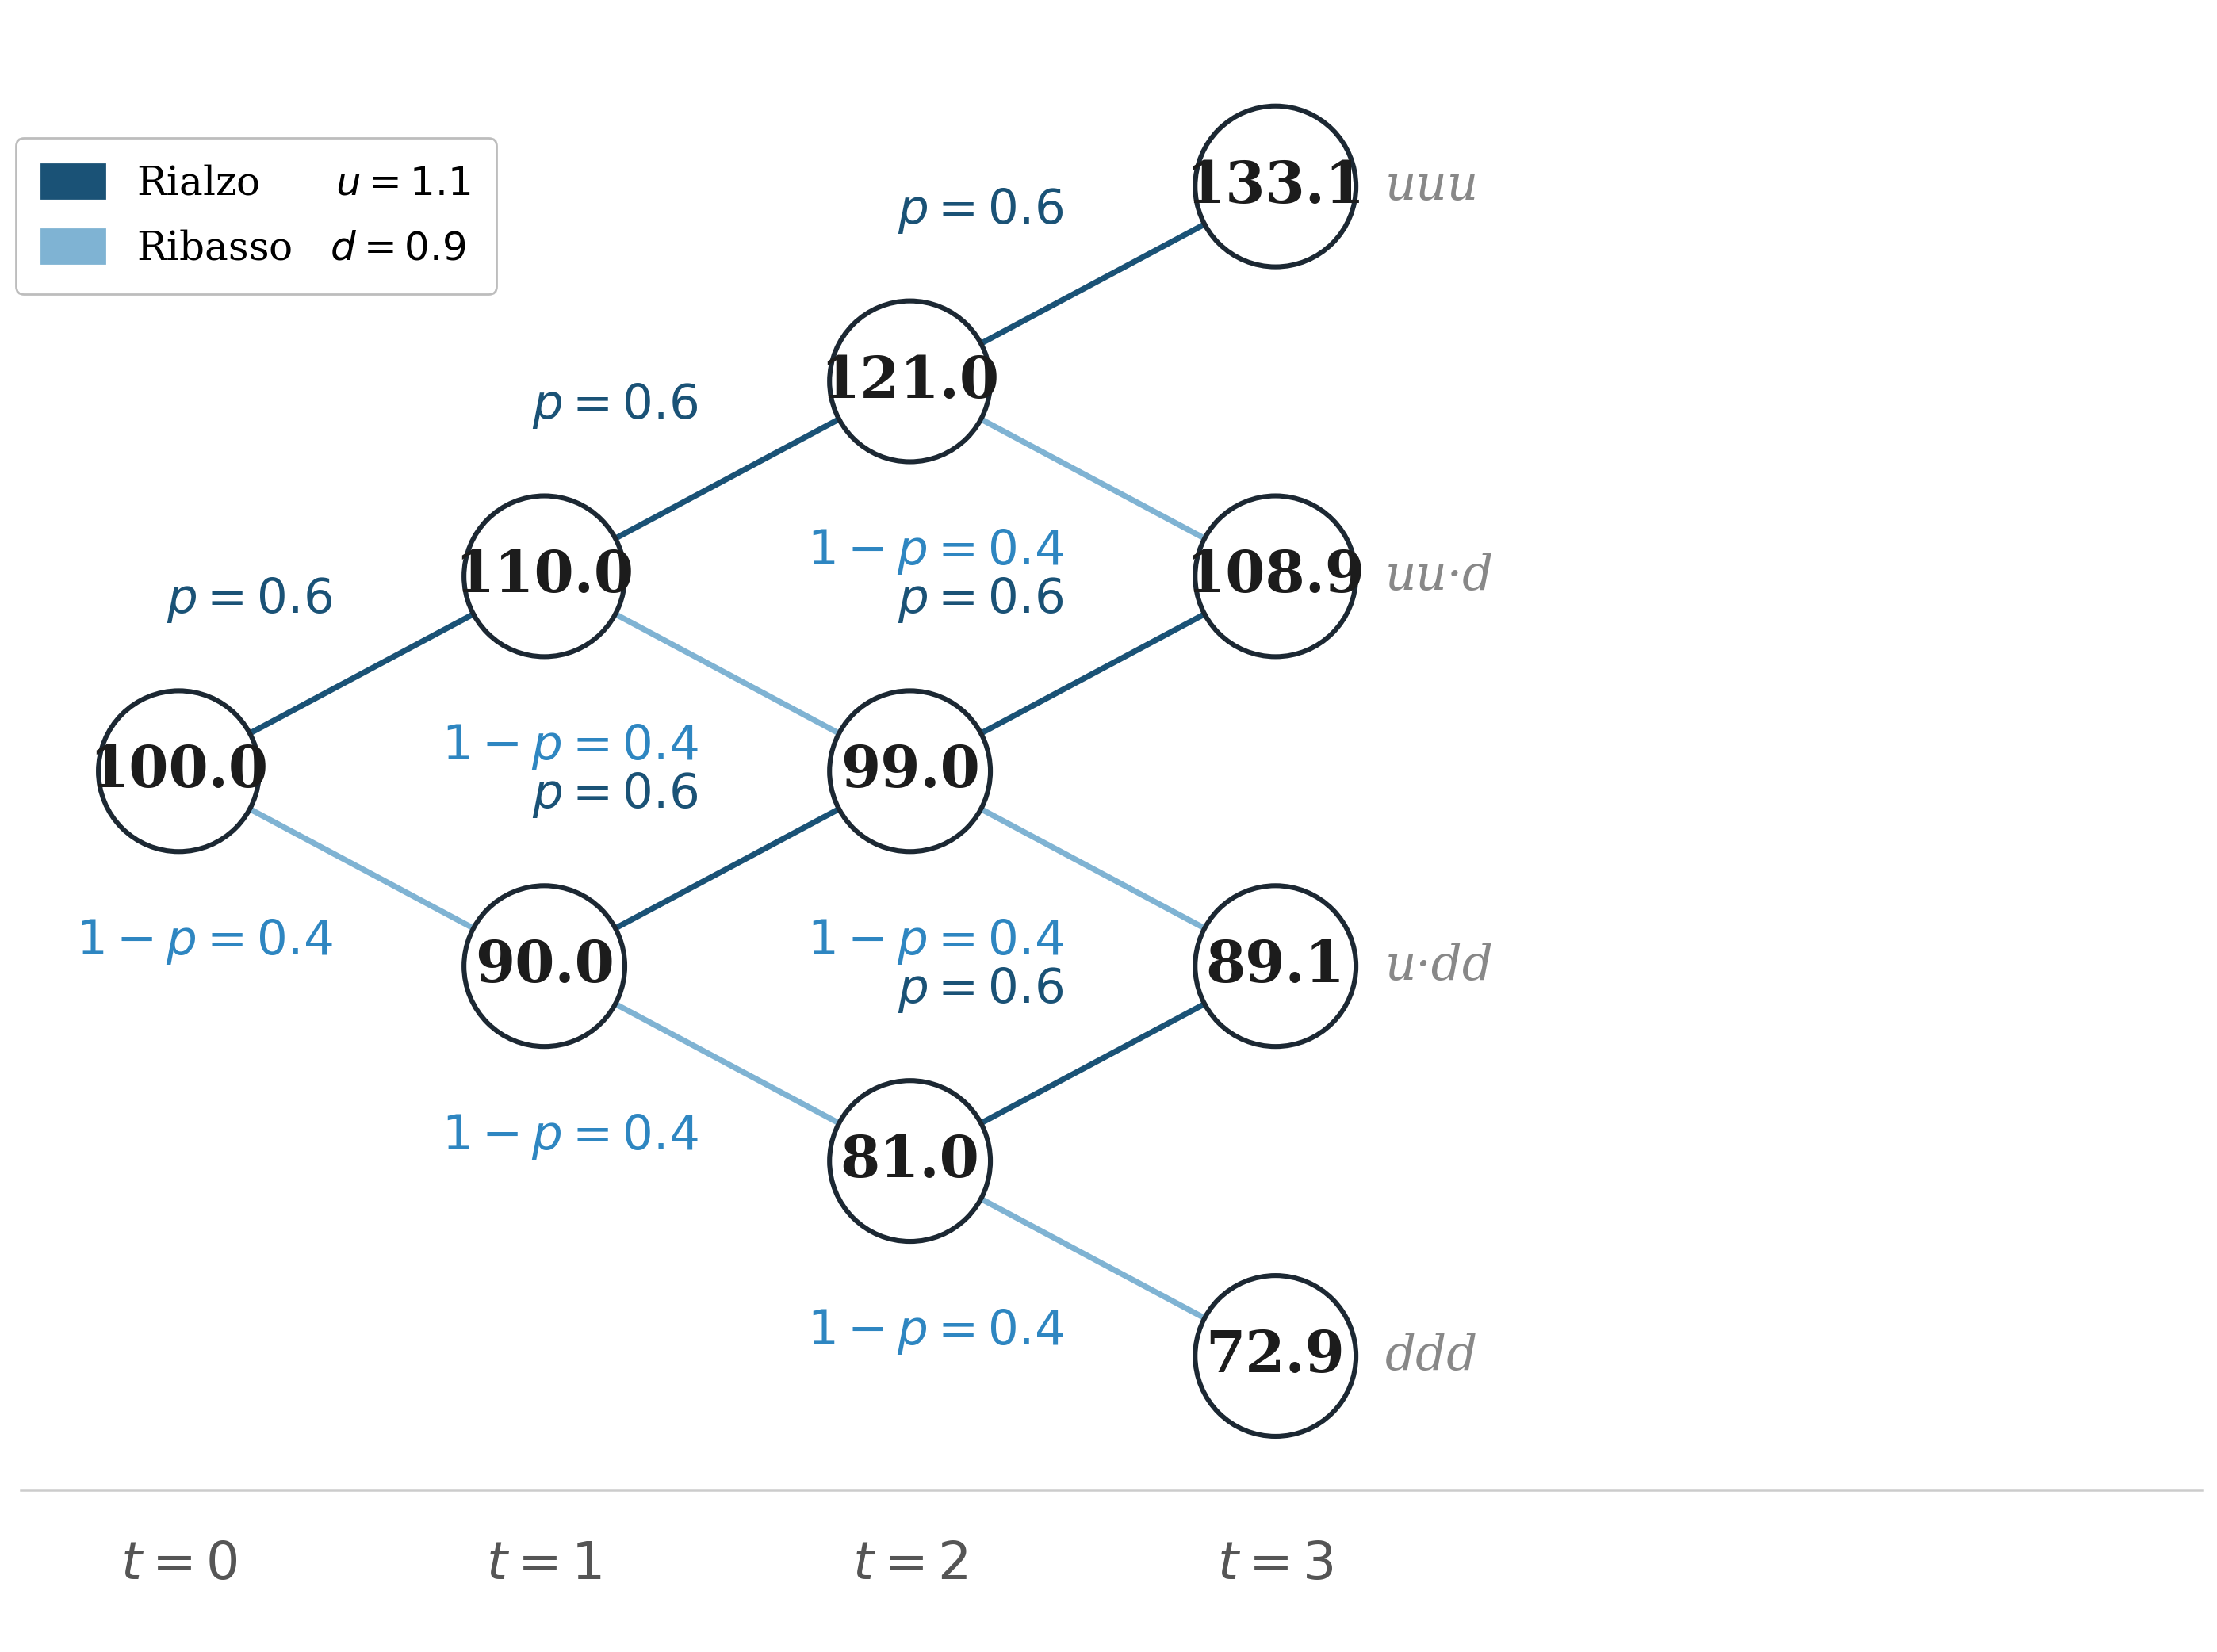
\includegraphics[width=0.92\textwidth]{../graphics/Cap04_Figura_4_1}
\caption{Albero binomiale dei prezzi con $S_0=100$, $u=1.1$,
$d=0.9$, $p=0.6$, $T=3$. Gli archi blu scuro indicano i movimenti
di rialzo (fattore $u$), gli archi azzurri quelli di ribasso
(fattore $d$). I nodi terminali corrispondono agli scenari
$s\in\mathcal{S}=\{1,\ldots,8\}$.}
\label{fig:albero-binomiale}
\end{figure}

La struttura ad albero rende visibili due propriet\`{a} fondamentali.
La prima \`{e} la \emph{non anticipativit\`{a}}: due traiettorie che
coincidono fino al tempo $t$ (cio\`{e} che passano per lo stesso nodo
al tempo $t$) non si distinguono sulla base dell'informazione $\F_t$.
La seconda \`{e} la \emph{ricombinazione}: nel modello binomiale,
poich\`{e} $ud=du$, traiettorie diverse che contengono lo stesso numero
di rialzi e ribassi raggiungono lo stesso nodo. Grazie a questa
propriet\`{a}, il numero di nodi distinti al tempo $t$ \`{e} $t+1$
anzich\`{e} $2^t$: i nodi crescono \emph{linearmente} con $t$, non
esponenzialmente. Per $T=3$ si hanno $4$ nodi terminali anzich\`{e}
$8$ traiettorie distinte, e il numero totale di nodi nell'albero \`{e}
$1+2+3+4=10$ anzich\`{e} $1+2+4+8=15$. Questa compressione \`{e}
computazionalmente cruciale: nei capitoli successivi consente di
calcolare prezzi e valori attesi condizionati su alberi con molti
passi in modo efficiente.

\begin{example}
\label{es:scenari-binomiale}
Per il modello con $S_0=100$, $u=1.1$, $d=0.9$, $p=0.6$, $T=3$, la
Tabella~\ref{tab:scenari-binomiale} elenca gli otto scenari con la
rispettiva probabilit\`{a} e il valore terminale.

\begin{table}[h]
\centering
\begin{tabular}{|c|c|c|c|}
\hline
\textbf{Scenario} $s$ & \textbf{Traiettoria} & $p_s$ & $S_3$\\
\hline
1 & $uuu$ & $0.216$ & $133.1$\\
2 & $uud$ & $0.144$ & $108.9$\\
3 & $udu$ & $0.144$ & $108.9$\\
4 & $duu$ & $0.144$ & $108.9$\\
5 & $udd$ & $0.096$ & $89.1$\\
6 & $dud$ & $0.096$ & $89.1$\\
7 & $ddu$ & $0.096$ & $89.1$\\
8 & $ddd$ & $0.064$ & $72.9$\\
\hline
\multicolumn{2}{|c|}{\textbf{Totale}} & $1.000$ & \\
\hline
\end{tabular}
\caption{Gli otto scenari del processo binomiale con $S_0=100$,
$u=1.1$, $d=0.9$, $p=0.6$, $T=3$.}
\label{tab:scenari-binomiale}
\end{table}
\end{example}


\begin{example}
\label{es:momenti-binomiale}
Per il processo binomiale con $S_0=100$, $u=1.1$, $d=0.9$, $p=0.6$,
$T=3$:
\[
m=0.6\cdot 1.1+0.4\cdot 0.9=1.02,
\qquad
m_2=0.6\cdot 1.21+0.4\cdot 0.81=1.050.
\]
I momenti del processo ai tre orizzonti sono riportati nella
Tabella~\ref{tab:momenti-binomiale}.

\begin{table}[h]
\centering
\begin{tabular}{|c|c|c|c|}
\hline
\textbf{Tempo} $t$ & $\mu(t)=\E[S_t]$ &
$\sigma^2(t)=\Var(S_t)$ & $\sigma(t)$\\
\hline
$0$ & $100.000$ & $0.000$ & $0.000$\\
$1$ & $102.000$ & $104.040$ & $10.200$\\
$2$ & $104.040$ & $215.523$ & $14.681$\\
$3$ & $106.121$ & $334.767$ & $18.297$\\
\hline
\end{tabular}
\caption{Media, varianza e deviazione standard del processo binomiale
($S_0=100$, $u=1.1$, $d=0.9$, $p=0.6$) ai tempi $t=0,1,2,3$. La
deviazione standard cresce con l'orizzonte: l'incertezza sul valore
futuro si accumula nel tempo, coerentemente con la struttura a
incrementi indipendenti.}
\label{tab:momenti-binomiale}
\end{table}

La covarianza tra $S_1$ e $S_3$ \`{e}:
\begin{eqnarray*}
\Cov(S_1,S_3)
&=& S_0^2\bigl(m_2^{\,1}\,m^{\,2}-m^{\,4}\bigr)\\
&=& 10000\,(1.050\cdot 1.0404-1.0824)\\
&=& 99.9,
\end{eqnarray*}
positiva, come atteso: prezzi elevati al tempo 1 tendono ad
accompagnarsi a prezzi elevati al tempo 3.
\end{example}



\subsection{L'incertezza cresce con l'orizzonte}

La Tabella~\ref{tab:momenti-binomiale} mostra che la deviazione
standard $\sigma(t)$ cresce al crescere di $t$. Questo fatto, che
nell'esempio \`{e} verificato numericamente, ha un significato
economico preciso: l'incertezza sul valore futuro di un'attivit\`{a}
finanziaria cresce con l'orizzonte di investimento.

\`{E} possibile quantificare questo effetto in modo esplicito. Per
il modello binomiale con incrementi i.i.d., si dimostra che la
deviazione standard cresce approssimativamente come $\sqrt{t}$ per
$t$ grande. Questo risultato \`{e} coerente con la propriet\`{a}
del moto browniano standard, per cui $\Var(W_t)=t$ e quindi
$\sigma(W_t)=\sqrt{t}$.

\begin{remark}
La crescita dell'incertezza con l'orizzonte ha implicazioni dirette
per la gestione del rischio. Il Value-at-Risk e il CVaR di una
posizione su un orizzonte di $T$ periodi non si ottengono
semplicemente moltiplicando per $T$ le misure di rischio a un
periodo: la struttura temporale della distribuzione delle perdite
deve essere modellata esplicitamente. Questo punto verr\`{a}
ripreso nel Capitolo~7.
\end{remark}


\subsection{Rendimenti logaritmici}

\noindent
\`{E} spesso conveniente descrivere il modello attraverso i
\emph{rendimenti logaritmici} anzich\`{e} i fattori moltiplicativi.
Si definisce
\[
r_t=\log\!\left(\frac{S_t}{S_{t-1}}\right)=\log R_t
\in\{\log u,\;\log d\}.
\]
Nel modello binomiale i rendimenti logaritmici $r_1,\ldots,r_T$ sono
indipendenti e identicamente distribuiti, con
\[
r_t=\begin{cases}
\log u & \text{con probabilit\`{a} }p,\\
\log d & \text{con probabilit\`{a} }1-p.
\end{cases}
\]
Il prezzo si scrive allora come esponenziale di una somma di
rendimenti logaritmici i.i.d.:
\[
S_t=S_0\exp\!\left(\sum_{k=1}^{t}r_k\right).
\]
Il logaritmo del prezzo, $\log S_t=\log S_0+\sum_{k=1}^{t}r_k$,
\`{e} dunque una passeggiata aleatoria nel senso
dell'Esempio~\ref{es:random-walk}. Questa osservazione anticipa il
legame tra il modello binomiale e il moto browniano geometrico: nel
Capitolo~6 vedremo che, facendo tendere a zero l'ampiezza del passo
temporale, la passeggiata aleatoria dei rendimenti logaritmici
converge a un moto browniano, e il modello binomiale dei prezzi al
corrispondente moto browniano geometrico.

\subsection{Sigma-algebra generata da una variabile casuale
e partizione di $\Omega$}

\noindent
Nel Capitolo~3 la sigma-algebra generata da una partizione
$\{B_1,\ldots,B_n\}$ di $\Omega$ era definita come l'insieme di tutti
gli eventi ottenibili come unioni dei blocchi $B_i$. Nella
Sezione~\ref{sec:momenti2} abbiamo introdotto la notazione
$\sigma(X_0,X_1,\ldots,X_t)$: la sigma-algebra \emph{generata da
variabili casuali}. Nel caso del modello binomiale \`{e} importante
verificare esplicitamente che le due notazioni descrivono lo stesso
oggetto, rendendo concreto e calcolabile il concetto generale.

La sigma-algebra $\sigma(X)$ generata da una variabile casuale $X$
che assume un numero finito di valori $v_1,\ldots,v_k$ coincide con
la sigma-algebra generata dalla partizione
\[
\bigl\{\{X=v_1\},\;\ldots,\;\{X=v_k\}\bigr\}.
\]
Conoscere il valore di $X$ equivale dunque a sapere in quale blocco
della partizione si trova l'esito $\omega$. La
Tabella~\ref{tab:sigma-partizione} mostra esplicitamente questa
corrispondenza per la filtrazione naturale del modello binomiale.

\begin{table}[h]
\centering
\begin{tabular}{|p{1.2cm}|p{3.5cm}|p{6.0cm}|}
\hline
\textbf{Tempo} $t$ & \textbf{Sigma-algebra} & \textbf{Partizione
corrispondente di $\Omega$}\\
\hline
$t=0$ & $\F_0=\sigma(S_0)=\{\emptyset,\Omega\}$ &
Unico blocco: \newline $\{uuu,uud,udu,udd,duu,dud,ddu,ddd\}$\\
\hline
$t=1$ & $\F_1=\sigma(S_1)$ &
Due blocchi: \newline $A_u=\{uuu,uud,udu,udd\}$ e \newline
$A_d=\{duu,dud,ddu,ddd\}$\\
\hline
$t=2$ & $\F_2=\sigma(S_1,S_2)$ &
Quattro blocchi: $A_{uu}=\{uuu,uud\}$,
$A_{ud}=\{udu,udd\}$,
$A_{du}=\{duu,dud\}$,
$A_{dd}=\{ddu,ddd\}$\\
\hline
$t=3$ & $\F_3=\sigma(S_1,S_2,S_3)$ &
Otto blocchi: ogni esito elementare forma un blocco
da solo, ad esempio $\{uuu\}$, $\{uud\}$, \ldots,
$\{ddd\}$\\
\hline
\end{tabular}
\caption{Sigma-algebre della filtrazione naturale del processo
binomiale ($S_0=100$, $u=1.1$, $d=0.9$, $T=3$) e partizioni
corrispondenti di $\Omega$. Ogni riga mostra come l'informazione
disponibile al tempo $t$ si traduca in una suddivisione di
$\Omega$ in blocchi indistinguibili sulla base delle osservazioni
fino a $t$.}
\label{tab:sigma-partizione}
\end{table}

\noindent
La tabella chiarisce che la notazione $\sigma(S_1,\ldots,S_t)$ non
aggiunge complessit\`{a} rispetto a quella del Capitolo~3: indica
semplicemente la sigma-algebra generata dalla partizione indotta dai
valori osservati del processo fino al tempo $t$.

\subsection{Filtrazione naturale e processo delle previsioni}

\noindent
La definizione generale di filtrazione naturale \`{e} stata introdotta
nella Sezione~\ref{sec:momenti2}. Nel modello binomiale essa ha una
struttura particolarmente trasparente: al tempo $t=0$ l'unica
informazione disponibile \`{e} quella banale, $\F_0=\{\emptyset,
\Omega\}$; al tempo $t=1$ si sa se il primo movimento \`{e} stato $u$
o $d$, e $\F_1$ distingue i due blocchi $A_u$ e $A_d$; al tempo $t=2$
si conoscono i primi due movimenti e $\F_2$ distingue quattro blocchi;
al tempo $t=3$ l'intera traiettoria \`{e} nota e $\F_3$ distingue
tutti e otto gli esiti.

Su questa filtrazione possiamo costruire concretamente il processo
delle previsioni introdotto in astratto nella
Sezione~\ref{sec:martingale}: la previsione del prezzo terminale
$S_3$ aggiornata all'informazione disponibile a ogni istante.

\begin{example}
\label{es:filtrazione-binomiale}
Nel processo binomiale con $S_0=100$, $u=1.1$, $d=0.9$, $p=0.6$,
$T=3$, calcoliamo il processo delle previsioni
$H_t=\E[S_3\mid\F_t]$ per $t=0,1,2,3$.

\paragraph{Una formula compatta.}
Poich\`{e} $S_3=S_t\cdot R_{t+1}\cdots R_3$ e i fattori futuri sono
indipendenti dall'informazione $\F_t$, con $\E[R_k]=m=1.02$:
\[
H_t=\E[S_3\mid\F_t]
=S_t\,\E[R_{t+1}\cdots R_3\mid\F_t]
=S_t\,m^{\,3-t}.
\]
La previsione del prezzo terminale \`{e} dunque il prezzo corrente
$S_t$ capitalizzato al rendimento medio $m$ per i periodi residui.

\paragraph{Calcolo nei due nodi al tempo $t=1$.}
Al tempo $t=1$ la filtrazione distingue il nodo $A_u$ (prezzo corrente
$S_1=110$) e il nodo $A_d$ ($S_1=90$). Verifichiamo la formula
compatta tramite il calcolo diretto. Per $\omega\in A_u$ i tre valori
terminali raggiungibili sono
\[
S_3=\begin{cases}
u^2\cdot 110=133.1 & \text{con probabilit\`{a} }p^2=0.36,\\
ud\cdot 110=108.9 & \text{con probabilit\`{a} }2p(1-p)=0.48,\\
d^2\cdot 110=89.1 & \text{con probabilit\`{a} }(1-p)^2=0.16,
\end{cases}
\]
da cui
\[
\E[S_3\mid A_u]=133.1\cdot 0.36+108.9\cdot 0.48+89.1\cdot 0.16
=114.444,
\]
in accordo con $S_1\,m^2=110\cdot 1.0404=114.444$. Analogamente, per
$\omega\in A_d$:
\[
\E[S_3\mid A_d]=108.9\cdot 0.36+89.1\cdot 0.48+72.9\cdot 0.16
=93.636=90\cdot 1.0404.
\]

\paragraph{Il processo delle previsioni sull'albero.}
Applicando la formula $H_t=S_t\,m^{\,3-t}$ a tutti i nodi si ottiene
il processo delle previsioni completo, riportato nella
Tabella~\ref{tab:previsioni-binomiale}.

\begin{table}[h]
\centering
\begin{tabular}{|c|l|}
\hline
\textbf{Tempo} $t$ & \textbf{Valori di } $H_t=\E[S_3\mid\F_t]$
\textbf{ nei nodi}\\
\hline
$0$ & $106.121$\\
$1$ & $114.444$ (nodo $u$), \quad $93.636$ (nodo $d$)\\
$2$ & $123.420$ (uu), \quad $100.980$ (ud), \quad $82.620$ (dd)\\
$3$ & $133.100$ (uuu), \quad $108.900$ (uud), \quad
       $89.100$ (udd), \quad $72.900$ (ddd)\\
\hline
\end{tabular}
\caption{Il processo delle previsioni $H_t=\E[S_3\mid\F_t]=S_t\,
m^{\,3-t}$ in tutti i nodi dell'albero binomiale. Al tempo $t=3$ la
previsione coincide con il valore realizzato $S_3$; al tempo $t=0$
coincide con la media incondizionata $\E[S_3]=106.121$.}
\label{tab:previsioni-binomiale}
\end{table}

\paragraph{Il processo delle previsioni \`{e} una martingala.}
Il processo $\{H_t\}$ \`{e} una martingala rispetto a $\{\F_t\}$, in
accordo con il risultato generale sulla martingala di Doob
(Sezione~\ref{sec:martingale}). Verifichiamolo su un passo, dal nodo
$u$ al tempo $1$ ai suoi due successori al tempo $2$ (i nodi uu e ud):
\[
\E[H_2\mid A_u]=0.6\cdot 123.420+0.4\cdot 100.980
=74.052+40.392=114.444=H_1(A_u).
\]
La previsione fatta oggi della previsione di domani coincide con la
previsione di oggi: le revisioni della previsione non sono prevedibili
in anticipo. In particolare, prendendo il valore atteso dal tempo $1$
al tempo $0$ si ritrova la propriet\`{a} della torre:
\[
\E[H_1]=0.6\cdot 114.444+0.4\cdot 93.636=106.121=\E[S_3].
\]

\paragraph{Attenzione: il processo dei prezzi non \`{e} una
martingala.} \`{E} importante non confondere il processo delle
previsioni $\{H_t\}$ con il processo dei prezzi $\{S_t\}$. Il primo
\`{e} sempre una martingala. Il secondo lo \`{e} solo se il rendimento
medio per periodo \`{e} unitario, $m=1$. Nel nostro esempio $m=1.02>1$,
e infatti
\[
\E[S_1\mid\F_0]=0.6\cdot 110+0.4\cdot 90=102=S_0\,m>S_0:
\]
il processo dei prezzi \`{e} una submartingala, coerentemente con il
fatto che un investimento azionario ha rendimento atteso positivo. La
condizione $m=1$, sotto la quale il prezzo diventa una martingala, ha
un ruolo centrale nella valutazione risk-neutral, che riprenderemo nei
capitoli dedicati al pricing.
\end{example}

% ============================================================
% MQF_Cap_05_Sezione_5_7.tex
% Capitolo 5 - Sezione 5.7
% Simulazione: logica generale e stima Monte Carlo
%
% Sezione nuova. Resta a livello generale (tempo discreto):
% niente modelli continui specifici ne' Eulero-Maruyama,
% che arrivano nel Capitolo 6.
% ============================================================

\section{Simulazione: logica generale e stima Monte Carlo}
\label{sec:simulazione}

\noindent
Molte quantit\`{a} di interesse in finanza --- il prezzo atteso di un
contratto, la perdita attesa di un portafoglio, la probabilit\`{a} di
superare una soglia di rischio --- si esprimono come valori attesi di
funzioni di un processo stocastico. In casi semplici, come il modello
binomiale della Sezione~\ref{sec:binomiale}, questi valori attesi si
calcolano in forma chiusa sommando su tutti gli scenari. Ma non appena
il numero di periodi cresce, o la dinamica del processo si fa pi\`{u}
complessa, l'enumerazione esplicita di tutti gli scenari diventa
impraticabile: un albero binomiale con $T=50$ periodi ha gi\`{a}
$2^{50}$ traiettorie, oltre mille miliardi. In questi casi si ricorre
alla \emph{simulazione}.

L'idea della simulazione \`{e} semplice e potente: invece di enumerare
tutti gli scenari possibili, se ne generano molti \emph{a caso},
coerentemente con la legge del processo, e si stima la quantit\`{a} di
interesse come media empirica sui soli scenari generati. Questa
sezione ne presenta la logica in forma generale, valida per qualunque
processo a tempo discreto. La sua applicazione ai modelli in tempo
continuo, mediante la discretizzazione delle equazioni differenziali
stocastiche, sar\`{a} sviluppata nel Capitolo~6 e implementata in
Python nella lezione applicativa.

\subsection{Generazione di traiettorie}

\noindent
Simulare un processo $\{X_t\}_{t=0}^{T}$ significa generare una
\emph{replica} della sua traiettoria, ovvero una sequenza di valori
$X_0^{(k)},X_1^{(k)},\ldots,X_T^{(k)}$ che costituisce una possibile
realizzazione del processo. Generando $M$ repliche indipendenti
\[
\bigl\{X_0^{(k)},X_1^{(k)},\ldots,X_T^{(k)}\bigr\},
\qquad k=1,2,\ldots,M,
\]
si ottiene un campione di $M$ traiettorie, ciascuna corrispondente a
un possibile percorso del processo.

Per un processo definito da una dinamica ricorsiva --- come il modello
binomiale, in cui $X_{t+1}$ si ottiene da $X_t$ applicando un
movimento aleatorio --- la generazione di una traiettoria procede in
modo sequenziale: si parte dal valore iniziale $X_0$, noto, e a ogni
passo si estrae l'innovazione casuale (nel caso binomiale, il
movimento $u$ o $d$) e si calcola il valore successivo. Ripetendo la
procedura per $T$ passi si ottiene un'intera traiettoria; ripetendola
per $M$ repliche indipendenti si ottiene il campione.

\begin{remark}
La fedelt\`{a} della simulazione dipende interamente dalla qualit\`{a}
del generatore di numeri casuali utilizzato per estrarre le
innovazioni. I generatori impiegati nella pratica sono in realt\`{a}
\emph{pseudo-casuali}: producono sequenze deterministiche che
imitano le propriet\`{a} statistiche dell'aleatoriet\`{a}. Questo ha
un risvolto utile: fissando il \emph{seme} (seed) del generatore, una
simulazione diventa esattamente riproducibile, il che \`{e}
essenziale per il controllo e la validazione dei risultati. Questo
aspetto operativo sar\`{a} ripreso nella lezione in Python.
\end{remark}

\subsection{La stima Monte Carlo}

\noindent
Supponiamo di voler calcolare il valore atteso $\E[g(X_T)]$ di una
funzione del processo --- ad esempio $g(X_T)=X_T$ per il valore atteso
terminale, oppure $g(X_T)=\max(X_T-K,0)$ per il payoff di un'opzione
call con prezzo di esercizio $K$. La \emph{stima Monte Carlo} di
questo valore atteso \`{e} la media empirica della funzione sulle $M$
traiettorie simulate:
\[
\widehat{\theta}_M=\frac{1}{M}\sum_{k=1}^{M}g\bigl(X_T^{(k)}\bigr).
\]
La giustificazione teorica di questa stima \`{e} la legge dei grandi
numeri, gi\`{a} incontrata nel Capitolo~2: poich\`{e} le repliche sono
indipendenti e identicamente distribuite, la media empirica converge
al valore atteso vero al crescere del numero di repliche,
\[
\widehat{\theta}_M\xrightarrow[M\to\infty]{}\theta=\E[g(X_T)].
\]
La simulazione Monte Carlo trasforma dunque il calcolo di un valore
atteso --- operazione che richiederebbe la conoscenza dell'intera
distribuzione di $g(X_T)$ --- in un semplice problema di media
campionaria, al prezzo di un errore di stima che, come vedremo,
si pu\`{o} controllare.

La stessa logica si applica a quantit\`{a} condizionate. La media di
$g(X_T)$ ristretta agli scenari che soddisfano una certa condizione
$A$ --- ad esempio gli scenari in cui il processo non scende mai sotto
una soglia --- si stima con
\[
\widehat{\theta}_M^{\,A}
=\frac{1}{M_A}\sum_{k:\,\omega^{(k)}\in A}g\bigl(X_T^{(k)}\bigr),
\qquad
M_A=\#\{k:\omega^{(k)}\in A\},
\]
ovvero come media della funzione sui soli scenari che ricadono in $A$,
dove $M_A$ \`{e} il numero di tali scenari.

\begin{example}[Stima del prezzo atteso terminale]
\label{es:montecarlo-binomiale}
Si consideri il modello binomiale con $S_0=100$, $u=1.1$, $d=0.9$,
$p=0.6$, $T=3$. Il valore atteso terminale esatto, calcolato nella
Sezione~\ref{sec:binomiale}, \`{e} $\E[S_3]=106.121$. Una simulazione
Monte Carlo lo stima generando $M$ traiettorie e mediando i valori
terminali $S_3^{(k)}$. Al crescere di $M$, la stima
$\widehat{\theta}_M$ si avvicina al valore esatto: con poche centinaia
di repliche l'approssimazione \`{e} gi\`{a} ragionevole, con alcune
decine di migliaia diventa accurata alle prime cifre decimali. In un
modello cos\`{\i} semplice la simulazione non \`{e} necessaria, poich\`{e}
il valore esatto \`{e} noto; ma essa fornisce un banco di prova ideale,
perch\`{e} permette di confrontare la stima simulata con il risultato
analitico e di verificare cos\`{\i} la correttezza della procedura ---
un passo di validazione che riprenderemo in Python.
\end{example}

\subsection{L'incertezza della stima}

\noindent
La stima Monte Carlo \`{e} essa stessa una quantit\`{a} aleatoria:
ripetendo l'intera simulazione con un diverso insieme di numeri
casuali si otterrebbe un valore leggermente diverso. \`{E} dunque
essenziale accompagnare la stima con una misura della sua incertezza.

Indichiamo con $\sigma_g^2=\Var\bigl(g(X_T)\bigr)$ la varianza della
quantit\`{a} simulata su una singola replica. Poich\`{e} la stima
$\widehat{\theta}_M$ \`{e} la media di $M$ repliche indipendenti, la
sua varianza \`{e}
\[
\Var\bigl(\widehat{\theta}_M\bigr)=\frac{\sigma_g^2}{M},
\]
e la sua deviazione standard --- detta \emph{errore standard} della
stima --- \`{e}
\[
\operatorname{SE}\bigl(\widehat{\theta}_M\bigr)
=\frac{\sigma_g}{\sqrt{M}}.
\]
Nella pratica $\sigma_g$ non \`{e} noto e si stima a sua volta dalla
deviazione standard campionaria delle repliche.

Questa formula racchiude la propriet\`{a} fondamentale --- e il limite
principale --- del metodo Monte Carlo: l'errore di stima decresce come
$1/\sqrt{M}$. Per dimezzare l'errore standard occorre quadruplicare il
numero di repliche; per guadagnare una cifra decimale di precisione
occorre moltiplicare per cento il numero di simulazioni. Questa
convergenza lenta \`{e} il prezzo della generalit\`{a} del metodo, ed
\`{e} la ragione per cui esistono numerose tecniche di
\emph{riduzione della varianza}, volte a diminuire $\sigma_g$ a
parit\`{a} di $M$, che la lezione in Python avr\`{a} modo di
illustrare.

\begin{remark}
Il fatto che l'errore decresca come $1/\sqrt{M}$, indipendentemente
dal numero di periodi $T$ o dalla complessit\`{a} del processo, \`{e}
ci\`{o} che rende la simulazione Monte Carlo cos\`{\i} preziosa nelle
applicazioni finanziarie. Mentre l'enumerazione esplicita degli
scenari ha un costo che cresce esponenzialmente con $T$, il costo
della simulazione cresce solo linearmente con $M$ e con $T$. \`{E}
per questo che la simulazione diventa il metodo di elezione non
appena la dimensione del problema supera la soglia in cui i metodi
esatti restano praticabili --- una situazione tipica nei modelli in
tempo continuo del prossimo capitolo, dove ogni traiettoria \`{e}
ottenuta discretizzando un'equazione differenziale stocastica su una
griglia temporale fitta.
\end{remark}

% ============================================================
% MQF_Cap_05_Sezione_5_8.tex
% Capitolo 5 - Sezione 5.8
% Esercizi svolti
%
% Formato soluzioni: \textbf{Soluzione.} + itemize
% (non si usa l'ambiente solution)
% ============================================================

\section{Esercizi svolti}
\label{sec:esercizi-svolti}

\begin{exercise}[Profitto cumulato di un desk di trading]
\label{ex:random-walk}
Un desk di trading realizza ogni giorno un profitto $Z_k$ che,
in migliaia di euro, assume due valori:
\[
Z_k=\begin{cases}
+3 & \text{con probabilit\`{a} }0.5,\\
-1 & \text{con probabilit\`{a} }0.5,
\end{cases}
\]
con i diversi giorni indipendenti e identicamente distribuiti. Il
profitto cumulato dopo $t$ giorni \`{e} $X_t=\sum_{k=1}^{t}Z_k$, con
$X_0=0$.
\begin{enumerate}
\item Calcolare media e varianza del profitto giornaliero (uguali per
ogni giorno, essendo le $Z_k$ i.i.d.).
\item Determinare le funzioni $\mu(t)=\E[X_t]$ e
$\sigma^2(t)=\Var(X_t)$.
\item Calcolare $\Cov(X_2,X_5)$.
\item Stabilire se $\{X_t\}$ \`{e} una martingala, una submartingala
o una supermartingala rispetto alla propria filtrazione naturale.
\end{enumerate}
\end{exercise}

\noindent
\textbf{Soluzione.}
\begin{enumerate}
\item Poich\'{e} le variabili $Z_1,Z_2,\ldots$ sono identicamente
distribuite, media e varianza non dipendono dall'indice: il calcolo
svolto per un generico tempo $k$ vale per ogni giorno. Per ogni
$k\geq 1$,
\[
\nu=\E[Z_k]=0.5\cdot 3+0.5\cdot(-1)=1.
\]
Per la varianza, sempre per ogni $k\geq 1$,
\[
\E[Z_k^2]=0.5\cdot 9+0.5\cdot 1=5,
\qquad
\tau^2=\Var(Z_k)=\E[Z_k^2]-\nu^2=5-1=4.
\]

\item Trattandosi di una passeggiata aleatoria con incrementi
i.i.d., per i risultati della Sezione~\ref{sec:momenti2}:
\[
\mu(t)=t\,\nu=t,
\qquad
\sigma^2(t)=t\,\tau^2=4t.
\]
La deviazione standard $\sigma(t)=2\sqrt{t}$ cresce con la radice
dell'orizzonte: l'incertezza sul profitto cumulato si accumula nel
tempo.

\item Per la struttura di covarianza della passeggiata aleatoria, con
$s\leq t$ vale $c(s,t)=\min(s,t)\,\tau^2$. Quindi
\[
\Cov(X_2,X_5)=\min(2,5)\cdot 4=2\cdot 4=8.
\]

\item Per $s\leq t$:
\[
\E[X_t\mid\F_s]=X_s+(t-s)\,\nu=X_s+(t-s)\geq X_s,
\]
con disuguaglianza stretta per $t>s$. Il processo \`{e} dunque una
\emph{submartingala}: il desk ha un vantaggio sistematico
($\nu=1>0$), e il profitto cumulato tende a crescere in media. Solo
se il profitto medio giornaliero fosse nullo il processo sarebbe una
martingala.
\end{enumerate}

\begin{exercise}[Albero binomiale a due periodi]
\label{ex:binomiale}
Un'azione vale oggi $S_0=80$. A ogni periodo il prezzo sale del
$25\%$ (fattore $u=1.25$) con probabilit\`{a} $p=0.5$, oppure scende
del $20\%$ (fattore $d=0.8$) con probabilit\`{a} $1-p=0.5$. Si
considera l'orizzonte $T=2$.
\begin{enumerate}
\item Costruire l'albero dei prezzi ed elencare gli scenari con le
rispettive probabilit\`{a}.
\item Calcolare $\E[S_2]$ e verificarlo con la formula
$\E[S_2]=S_0\,m^2$.
\item Calcolare $\E[S_2\mid\F_1]$ nei due nodi al tempo $1$ e
verificare la propriet\`{a} della torre.
\end{enumerate}
\end{exercise}

\noindent
\textbf{Soluzione.}
\begin{enumerate}

\item Il rendimento lordo medio per periodo \`{e}
\[
m=pu+(1-p)d=0.5\cdot 1.25+0.5\cdot 0.8=1.025.
\]
I valori del prezzo nei nodi sono:
\[
\begin{array}{ll}
t=0: & S_0=80;\\
t=1: & S_1^u=80\cdot 1.25=100, \quad S_1^d=80\cdot 0.8=64;\\
t=2: & S_2^{uu}=125, \quad S_2^{ud}=S_2^{du}=80,
       \quad S_2^{dd}=51.2.
\end{array}
\]
I quattro scenari, con probabilit\`{a} $p_s=0.25$ ciascuno (essendo
$p=0.5$), sono: $uu$ con $S_2=125$; $ud$ e $du$ con $S_2=80$; $dd$ con
$S_2=51.2$.

\item Sommando sugli scenari:
\[
\E[S_2]=0.25\cdot 125+0.5\cdot 80+0.25\cdot 51.2
=31.25+40+12.8=84.05.
\]
La formula compatta conferma: $\E[S_2]=S_0\,m^2=80\cdot
1.025^2=80\cdot 1.050625=84.05$.

\item Al nodo $u$ ($S_1=100$), i due esiti al tempo $2$ sono $125$ e
$80$, ciascuno con probabilit\`{a} $0.5$:
\[
\E[S_2\mid A_u]=0.5\cdot 125+0.5\cdot 80=102.5=100\cdot 1.025.
\]
Al nodo $d$ ($S_1=64$), gli esiti sono $80$ e $51.2$:
\[
\E[S_2\mid A_d]=0.5\cdot 80+0.5\cdot 51.2=65.6=64\cdot 1.025.
\]
Verifica della torre:
\[
\E\bigl[\E[S_2\mid\F_1]\bigr]
=0.5\cdot 102.5+0.5\cdot 65.6=51.25+32.8=84.05=\E[S_2].
\]
\end{enumerate}

\begin{exercise}[Prezzo scontato e misura di martingala]
\label{ex:scontato}
Si consideri un periodo singolo. Un'azione vale $S_0=100$ e tra un
periodo varr\`{a} $S_1=120$ (rialzo) oppure $S_1=90$ (ribasso). Il
tasso privo di rischio per il periodo \`{e} $r=0.05$. Si definisca la
probabilit\`{a} di rialzo $q$ in modo che il prezzo scontato
$\tilde{S}_t=S_t/(1+r)^t$ sia una martingala, cio\`{e} tale che
$\E_{\Q}[\tilde{S}_1]=\tilde{S}_0=S_0$.
\begin{enumerate}
\item Determinare il valore di $q$.
\item Verificare che, sotto tale probabilit\`{a}, il prezzo scontato
soddisfa la propriet\`{a} di martingala.
\item Interpretare il risultato.
\end{enumerate}
\end{exercise}

\noindent
\textbf{Soluzione.}
\begin{enumerate}
\item La condizione di martingala per il prezzo scontato su un periodo
\`{e}
\[
\frac{1}{1+r}\,\E_{\Q}[S_1]=S_0,
\qquad\text{ossia}\qquad
\E_{\Q}[S_1]=S_0(1+r).
\]
Con $\E_{\Q}[S_1]=q\cdot 120+(1-q)\cdot 90$ e $S_0(1+r)=105$:
\[
120q+90(1-q)=105
\;\Longrightarrow\;
30q=15
\;\Longrightarrow\;
q=0.5.
\]
In generale $q=\dfrac{(1+r)S_0-S_1^d}{S_1^u-S_1^d}
=\dfrac{105-90}{120-90}=0.5$, formula che riprenderemo nei capitoli
sul pricing.

\item Sotto $\Q$ con $q=0.5$:
\[
\E_{\Q}[\tilde{S}_1]
=\frac{1}{1.05}\bigl(0.5\cdot 120+0.5\cdot 90\bigr)
=\frac{105}{1.05}=100=\tilde{S}_0.
\]
Il prezzo scontato \`{e} dunque una martingala sotto $\Q$.

\item La probabilit\`{a} $q=0.5$ non \`{e} la probabilit\`{a}
\emph{fisica} con cui il mercato sale o scende, ma una probabilit\`{a}
\emph{artificiale} --- la misura risk-neutral $\Q$ --- costruita in
modo che il prezzo scontato dell'azione diventi una martingala. Sotto
questa misura, ogni attivit\`{a} ha rendimento atteso pari al tasso
privo di rischio. \`{E} questa la propriet\`{a} che, nei capitoli sul
pricing, consentir\`{a} di valutare un derivato come valore atteso
scontato del suo payoff sotto $\Q$.
\end{enumerate}

\begin{exercise}[Dimensionamento di una simulazione Monte Carlo]
\label{ex:montecarlo}
Si vuole stimare per simulazione il prezzo atteso $\theta=\E[g(X_T)]$
di un contratto. Una simulazione pilota con $M_0=1\,000$ repliche
fornisce una stima $\widehat{\theta}=12.4$ e una deviazione standard
campionaria delle repliche pari a $s_g=15$.
\begin{enumerate}
\item Stimare l'errore standard della stima pilota e costruire un
intervallo di confidenza approssimato al $95\%$ per $\theta$.
\item Determinare il numero di repliche necessario affinch\'{e}
l'errore standard scenda a $0.05$.
\end{enumerate}
\end{exercise}

\noindent
\textbf{Soluzione.}
\begin{enumerate}
\item L'errore standard della stima pilota \`{e}
\[
\operatorname{SE}=\frac{s_g}{\sqrt{M_0}}
=\frac{15}{\sqrt{1\,000}}
=\frac{15}{31.62}\approx 0.474.
\]
Un intervallo di confidenza approssimato al $95\%$, usando il
quantile $1.96$ della normale standard, \`{e}
\[
\widehat{\theta}\pm 1.96\cdot\operatorname{SE}
=12.4\pm 1.96\cdot 0.474
=12.4\pm 0.93,
\]
ossia all'incirca l'intervallo $[11.47,\;13.33]$.

\item Imponendo $\operatorname{SE}=s_g/\sqrt{M}\leq 0.05$ e
risolvendo per $M$:
\[
\sqrt{M}\geq\frac{s_g}{0.05}=\frac{15}{0.05}=300
\;\Longrightarrow\;
M\geq 300^2=90\,000.
\]
Per ridurre l'errore standard da $0.474$ a $0.05$, ovvero di un
fattore circa $9.5$, occorre aumentare il numero di repliche di un
fattore $9.5^2\approx 90$: dalle mille repliche iniziali a circa
novantamila. Questo illustra concretamente la convergenza $1/\sqrt{M}$
del metodo Monte Carlo, e il motivo per cui, quando l'accuratezza
richiesta \`{e} elevata, diventano interessanti le tecniche di
riduzione della varianza.
\end{enumerate}

% ============================================================
% MQF_Cap_05_Sezione_5_9.tex
% Capitolo 5 - Sezione 5.9
% Esercizi proposti
%
% Sei esercizi di difficolta' crescente. Per ciascuno e' indicato
% il solo risultato finale, per l'autovalutazione (puo' essere
% rimosso se si preferisce non fornirlo).
% ============================================================

\section{Esercizi proposti}
\label{sec:esercizi-proposti}

\begin{exercise}[Posizione di cassa aleatoria]
\label{ex:prop-rw}
La posizione di cassa giornaliera di un'attivit\`{a} varia ogni giorno
di una quantit\`{a} $Z_k$ che vale $+2$ con probabilit\`{a} $0.6$ e
$-2$ con probabilit\`{a} $0.4$ (in migliaia di euro), con giorni
indipendenti. Sia $X_t=\sum_{k=1}^{t}Z_k$ la posizione cumulata,
$X_0=0$.
\begin{enumerate}
\item Calcolare media e varianza di $Z_k$.
\item Determinare $\mu(t)$ e $\sigma(t)$, e calcolare i loro valori
per $t=10$.
\item Stabilire se $\{X_t\}$ \`{e} martingala, submartingala o
supermartingala.
\end{enumerate}
\textit{Risultati:} $\nu=0.4$, $\tau^2=3.84$; $\mu(10)=4$,
$\sigma(10)\approx 6.20$; submartingala.
\end{exercise}

\begin{exercise}[Albero binomiale a tre periodi]
\label{ex:prop-binomiale}
Un'azione vale $S_0=50$. A ogni periodo sale del $20\%$ ($u=1.2$) con
probabilit\`{a} $p=0.55$, oppure scende del $10\%$ ($d=0.9$) con
probabilit\`{a} $0.45$. Si consideri $T=3$.
\begin{enumerate}
\item Determinare i quattro valori terminali distinti di $S_3$ e le
loro probabilit\`{a}.
\item Calcolare $\E[S_3]$, sia sommando sugli scenari sia con la
formula $S_0\,m^3$.
\item Calcolare la deviazione standard $\sigma(3)$.
\end{enumerate}
\textit{Risultati:} $m=1.065$; valori terminali $86.40$, $64.80$,
$48.60$, $36.45$; $\E[S_3]\approx 60.40$.
\end{exercise}

\begin{exercise}[Processi adattati e anticipativi]
\label{ex:prop-adattato}
Sia $\{S_t\}_{t=0}^{T}$ un processo dei prezzi con filtrazione
naturale $\{\F_t\}$. Per ciascuno dei seguenti processi, stabilire se
\`{e} adattato o anticipativo rispetto a $\{\F_t\}$, motivando la
risposta:
\begin{enumerate}
\item $Y_t=\tfrac{1}{2}(S_t+S_{t-1})$, la media tra prezzo corrente e
prezzo del periodo precedente;
\item $Y_t=S_{t+1}-S_t$, la variazione del periodo successivo;
\item $Y_t=\min_{0\leq s\leq t}S_s$, il prezzo minimo osservato fino
a $t$;
\item $Y_t=\E[S_T\mid\F_t]$, la previsione del prezzo terminale.
\end{enumerate}
\textit{Risultati:} adattati i processi (1), (3) e (4); anticipativo
il processo (2).
\end{exercise}

\begin{exercise}[Processo delle previsioni e torre]
\label{ex:prop-previsioni}
Si riprenda l'azione dell'Esercizio~\ref{ex:prop-binomiale}
($S_0=50$, $u=1.2$, $d=0.9$, $p=0.55$, $T=3$). Si consideri il
processo delle previsioni $H_t=\E[S_3\mid\F_t]$.
\begin{enumerate}
\item Usando la formula compatta $H_t=S_t\,m^{\,3-t}$, calcolare il
valore di $H_2$ nei tre nodi al tempo $t=2$.
\item Verificare la propriet\`{a} di martingala passando dal nodo
$uu$ al tempo $2$ ai suoi successori al tempo $3$.
\end{enumerate}
\textit{Risultati:} $S_2$ nei tre nodi $=72$, $54$, $40.5$; quindi
$H_2=76.68$, $57.51$, $43.13$.
\end{exercise}

\begin{exercise}[Condizione di martingala per i prezzi]
\label{ex:prop-martingala}
In un modello binomiale i fattori sono $u=1.1$ e $d=0.95$. Si
determini la probabilit\`{a} di rialzo $p$ che rende il processo dei
prezzi $\{S_t\}$ una martingala rispetto alla propria filtrazione
naturale. Interpretare il risultato confrontandolo con il rendimento
atteso di un investimento azionario reale.

\smallskip
\textit{Risultato:} la condizione \`{e} $m=pu+(1-p)d=1$, da cui
$p=1/3$. Poich\'{e} un'azione reale ha rendimento atteso positivo
($m>1$), la probabilit\`{a} fisica \`{e} in genere maggiore di $1/3$:
il prezzo \`{e} una submartingala sotto la misura fisica.
\end{exercise}

\begin{exercise}[Precisione di una stima Monte Carlo]
\label{ex:prop-montecarlo}
Per stimare il prezzo atteso di un contratto si esegue una simulazione
con $M=2\,500$ repliche, ottenendo una stima $\widehat{\theta}=18.7$
e una deviazione standard campionaria $s_g=8$.
\begin{enumerate}
\item Calcolare l'errore standard della stima e un intervallo di
confidenza approssimato al $95\%$.
\item Determinare il numero di repliche necessario per portare
l'errore standard a $0.02$.
\end{enumerate}
\textit{Risultati:} $\operatorname{SE}=0.16$, intervallo
$18.7\pm 0.314$; servono $M=160\,000$ repliche.
\end{exercise}

% ============================================================
% MQF_Cap_05_Sezione_5_10.tex
% Capitolo 5 - Sezione 5.10
% Sintesi e ponte verso il Capitolo 6
%
% NOTA: la sintesi NON cita i casi d'uso specifici del Cap. 6
% (opzioni asiatiche, OU, CIR, obbligazioni indicizzate).
% ============================================================

\section{Sintesi}
\label{sec:sintesi-cap5}

\noindent
Questo capitolo ha introdotto il linguaggio dei processi stocastici e
gli strumenti per descriverne il comportamento nel tempo. Conviene
ripercorrere i concetti principali, raggruppati per funzione, prima di
indicare come essi verranno utilizzati nel seguito del corso.

\subsection{I concetti fondamentali}

\noindent
Il capitolo si \`{e} sviluppato lungo tre direttrici.

\paragraph{1. La descrizione di un processo.}
Un processo stocastico $\{X_t\}_{t\in\mathcal{T}}$ \`{e} una famiglia
di variabili casuali indicizzata dal tempo, leggibile a tre livelli:
la distribuzione marginale a un istante fissato, la traiettoria per un
esito fissato, la famiglia nel suo complesso. La sua struttura
temporale si descrive sinteticamente mediante la funzione media
$\mu(t)$, la funzione varianza $\sigma^2(t)$ e la funzione di
autocovarianza $c(s,t)$, e si caratterizza attraverso le propriet\`{a}
degli incrementi --- indipendenza e stazionariet\`{a} --- e le
nozioni di stazionariet\`{a} del processo.

\paragraph{2. L'informazione e la sua evoluzione.}
Il flusso progressivo dell'informazione si formalizza mediante una
filtrazione $\{\F_t\}$, successione crescente di sigma-algebre. Un
processo \`{e} adattato se il suo valore a ogni istante \`{e}
osservabile con l'informazione disponibile in quell'istante; \`{e}
anticipativo in caso contrario. Solo i processi adattati descrivono
quantit\`{a} e strategie effettivamente implementabili.

\paragraph{3. Le martingale.}
Una martingala formalizza l'idea di gioco equo: la migliore previsione
del valore futuro coincide con il valore presente. Submartingale e
supermartingale descrivono giochi rispettivamente favorevoli e
sfavorevoli. Il processo delle previsioni di una qualunque quantit\`{a}
terminale \`{e} sempre una martingala, e la propriet\`{a} di martingala
del prezzo scontato, sotto un'opportuna misura, \`{e} il fondamento
della valutazione dei derivati.

La Tabella~\ref{tab:sintesi-cap5} raccoglie questi concetti con la
notazione introdotta e il loro significato.

\begin{table}[h]
\centering
\begin{tabular}{|p{2.5cm}|p{3.8cm}|p{4.5cm}|}
\hline
\textbf{Concetto} & \textbf{Notazione} & \textbf{Significato}\\
\hline
Processo stocastico & $\{X_t\}_{t\in\mathcal{T}}$ &
Famiglia di variabili casuali indicizzata dal tempo\\
\hline
Traiettoria & $t\mapsto X_t(\omega)$ &
Realizzazione del processo per un esito fissato\\
\hline
Funzione media & $\mu(t)=\E[X_t]$ &
Livello medio del processo nel tempo\\
\hline
Autocovarianza & $c(s,t)=\Cov(X_s,X_t)$ &
Dipendenza lineare tra istanti diversi\\
\hline
Filtrazione & $\{\F_t\}$ &
Flusso crescente dell'informazione\\
\hline
Processo adattato & $X_t$ $\F_t$-misurabile &
Quantit\`{a} osservabile al tempo $t$\\
\hline
Martingala & $\E[X_t\mid\F_s]=X_s$ &
Gioco equo; previsione $=$ valore presente\\
\hline
Scenario & $s\in\mathcal{S}$, $p_s$, $\xi_s$ &
Traiettoria discreta con la sua probabilit\`{a}\\
\hline
Stima Monte Carlo &
$\widehat{\theta}_M=\frac{1}{M}\sum_k g(X_T^{(k)})$ &
Media empirica su $M$ traiettorie simulate\\
\hline
\end{tabular}
\caption{Sintesi dei concetti del Capitolo~5.}
\label{tab:sintesi-cap5}
\end{table}

\subsection{Il modello binomiale come palestra}

\noindent
Tutti questi concetti, introdotti in forma generale, sono stati
applicati a un modello concreto --- il modello binomiale dei prezzi
--- scelto per la possibilit\`{a} di svolgere ogni calcolo
esplicitamente e di visualizzare la struttura del processo mediante
l'albero degli scenari. Su questo modello abbiamo calcolato momenti,
costruito la filtrazione naturale, verificato la propriet\`{a} della
torre e illustrato il processo delle previsioni come martingala. Il
modello binomiale ha cos\`{\i} svolto la funzione di banco di prova
dei concetti generali, su un caso in cui ogni risultato pu\`{o} essere
controllato a mano.

\subsection{Verso i modelli in tempo continuo}

\noindent
Gli strumenti sviluppati in questo capitolo --- processo, traiettoria,
momenti, filtrazione, martingala, scenario, simulazione --- non sono
legati al tempo discreto: sono stati definiti in modo da valere per
qualunque insieme di indici temporali. Il capitolo successivo li
applicher\`{a} ai \emph{processi in tempo continuo}, in cui il tempo
varia con continuit\`{a} e le traiettorie diventano funzioni definite
su un intervallo.

Il passaggio al tempo continuo non \`{e} un mero raffinamento tecnico.
\`{E} il linguaggio in cui sono formulati i principali modelli per i
prezzi delle attivit\`{a}, per i tassi di interesse e per i fattori di
rischio, ed \`{e} il contesto naturale per le applicazioni di
simulazione e valutazione che costituiscono il cuore operativo della
parte successiva del corso. Vedremo come la passeggiata aleatoria
incontrata in questo capitolo abbia un analogo continuo --- il moto
browniano --- e come da esso si costruiscano, con l'aggiunta di
opportune componenti di tendenza e di richiamo verso un livello di
equilibrio, i modelli usati nella pratica finanziaria. Lo strumento
della simulazione Monte Carlo, introdotto qui in forma generale,
diventer\`{a} in quel contesto il metodo operativo per generare
traiettorie e stimare quantit\`{a} di interesse, una volta che le
equazioni dei modelli in tempo continuo siano state discretizzate su
una griglia temporale.

}}%
%BeginExpansion
%2multibyte Version: 5.50.0.2960 CodePage: 65001
% MQF_Manuale_Master_SW55_Memoir.tex
% Master del manuale MQF costruito sullo shell SW5.5 "Memoir Class for Configurable Typesetting".
% Versione modulare: i capitoli scritti sono inclusi con \input.%
% POSIZIONE DEI FILE
% Questo master deve stare nella cartella 01_Manuale.
% I capitoli devono stare nella sottocartella 01_Manuale/Capitoli.
% Non mettere il master dentro Capitoli.
% I capitoli futuri restano come traccia, ma non generano pagine nel documento.
% Evita pagine bianche dovute all'apertura dei capitoli su pagina dispari.
% ------------------------------------------------------------
% Nomi italiani
% ------------------------------------------------------------
% ------------------------------------------------------------
% Macro matematiche ufficiali del progetto MQF
% Coerenti con MQF_Notazione.tex
% ------------------------------------------------------------
% ------------------------------------------------------------
% Ambienti di tipo teorema.
% I nomi interni restano compatibili con lo shell SW.
% Le etichette stampate sono in italiano.
% ------------------------------------------------------------

%TCIDATA{OutputFilter=latex2.dll}
%TCIDATA{Version=5.50.0.2960}
%TCIDATA{LaTeXparent=1,1,MQF_Manuale_Master.tex}


% Capitoli/MQF_Cap_05_Processi_stocastici_in_tempo_discreto.tex

\chapter[Processi stocastici, Tempo Discreto]{Processi stocastici, traiettorie e scenari}

\label{cap:processi}

\section{Obiettivi della lezione}

Nei capitoli precedenti l'incertezza \`{e} stata rappresentata mediante
variabili casuali definite su uno spazio di probabilit\`{a}
$(\Omega,\F,\Prob)$. Una variabile casuale $X$ descrive una grandezza
aleatoria in un singolo momento: il rendimento di un titolo alla fine di un
periodo, il payoff terminale di un contratto, la perdita di un portafoglio su
un orizzonte fissato. Il Capitolo~3 ha mostrato come l'arrivo di nuova
informazione modifichi la valutazione di $X$, introducendo il valore atteso
condizionato $\E[X\mid\G]$ e anticipando la struttura di una filtrazione
$\{\F_t\}_{t=0}^{T}$ come successione crescente di sigma-algebre
informative.

In molte applicazioni finanziarie, tuttavia, non interessa una singola
grandezza aleatoria, ma la sua evoluzione nel tempo. Il prezzo di
un'attivit\`{a} finanziaria varia di giorno in giorno; il merito creditizio
di una controparte si modifica nel corso degli anni; un fattore di rischio
macroeconomico si aggiorna a ogni nuova pubblicazione di dati. Per descrivere
queste evoluzioni \`{e} necessario un oggetto pi\`{u} ricco di una singola
variabile casuale: il \emph{processo stocastico}.

Lo studio dei processi stocastici si articola, in questo corso, su due
capitoli complementari. Il presente capitolo \`{e} dedicato ai
\emph{fondamenti}: introduce il linguaggio generale dei processi ---
traiettoria, scenario, legge, momenti, dipendenza temporale ---, gli
strumenti per descrivere il flusso dell'informazione --- filtrazione e
adattabilit\`{a} --- e il concetto di martingala, che formalizza l'idea
di gioco equo e costituisce il fondamento della valutazione dei
derivati. Questi strumenti valgono per qualunque processo, a tempo
discreto o continuo, e costituiscono il vocabolario di base
dell'intero corso. Il capitolo li illustra poi su un primo modello
concreto in tempo discreto, il modello binomiale, scelto per la sua
semplicit\`{a} e per la possibilit\`{a} di svolgere ogni calcolo in
modo esplicito.
 
Il capitolo successivo si appogger\`{a} interamente su queste basi per
sviluppare i modelli in tempo continuo --- moto browniano geometrico,
processi mean-reverting, diffusioni multivariate --- che la lezione
applicativa in Python utilizzer\`{a} per la simulazione di traiettorie
e per la valutazione di opzioni asiatiche e obbligazioni indicizzate
all'inflazione.

Al termine di questo capitolo lo studente dovr\`{a} essere in grado di:
 
\begin{itemize}
 
\item definire un processo stocastico, distinguere il suo insieme di
indici temporali e il suo spazio degli stati, e leggere lo stesso
oggetto ai tre livelli: distribuzione marginale per ogni $t$ fissato,
traiettoria per ogni $\omega$ fissato, famiglia indicizzata dal tempo;
 
\item descrivere un processo attraverso la funzione media $\mu(t)$, la
funzione varianza $\sigma^2(t)$ e la funzione di autocovarianza
$c(s,t)$, e riconoscere le propriet\`{a} di stazionariet\`{a} e di
indipendenza degli incrementi;
 
\item costruire la filtrazione naturale di un processo e distinguere
un processo adattato da un processo anticipativo, con riferimento alle
strategie finanziarie implementabili;
 
\item definire una martingala rispetto a una filtrazione, riconoscere
submartingale e supermartingale, e interpretarle in termini di gioco
equo, favorevole o sfavorevole;
 
\item costruire il modello binomiale dei prezzi, calcolarne i momenti,
elencarne gli scenari mediante l'albero e calcolare valori attesi
condizionati lungo il processo;
 
\item descrivere la logica della simulazione per scenari e la stima
Monte Carlo di una quantit\`{a} attesa, valutandone l'incertezza.

\end{itemize}

Il capitolo prepara il passaggio ai modelli in tempo continuo
(Capitolo~6), alle catene di Markov (Capitoli~8 e~9) e alla
programmazione stocastica per scenari (Capitoli~14 e~15). In tutti
questi contesti, i concetti introdotti qui costituiranno lo strumento
di modellizzazione fondamentale.


\section{Motivazione finanziaria}

\subsection{Dal dato statico all'evoluzione temporale}

Immaginiamo un gestore di portafoglio che ogni mattina osserva il prezzo
di chiusura del giorno precedente per un titolo azionario. Dopo trenta
giorni di osservazioni dispone di una sequenza di trenta valori: non una
singola quantit\`{a} aleatoria, ma un'evoluzione temporale dell'incertezza.
Le domande che si pone naturalmente sono diverse da quelle affrontate nei
capitoli precedenti.

\begin{itemize}

\item Le variazioni di prezzo di giorni successivi sono indipendenti tra
loro, oppure un rialzo oggi rende pi\`{u} probabile un rialzo anche domani?

\item Sapere che il prezzo ha raggiunto un certo livello oggi modifica la
previsione del prezzo tra una settimana?

\item Come si rappresentano tutti i percorsi possibili del prezzo su un
orizzonte di tre mesi, e con quali probabilit\`{a}?

\item Come cresce l'incertezza sul valore futuro del portafoglio al
prolungarsi dell'orizzonte di investimento?

\end{itemize}

Nessuna di queste domande pu\`{o} essere formulata in modo preciso usando
soltanto le variabili casuali dei capitoli precedenti. Serve un oggetto
matematico che descriva simultaneamente l'incertezza a ogni istante
temporale e la struttura di dipendenza tra istanti diversi: il
\emph{processo stocastico}.

La stessa esigenza si presenta in contesti diversi ma strutturalmente
analoghi. Il merito creditizio di un'impresa si modifica nel tempo,
passando da una classe di rating a un'altra in risposta all'evoluzione
del ciclo economico e della situazione patrimoniale dell'emittente. Il
tasso di interesse a breve termine oscilla attorno a un livello di
equilibrio di lungo periodo, con variazioni giornaliere che dipendono
dalle decisioni di politica monetaria e dalle aspettative del mercato.
La perdita cumulata di un portafoglio creditizio si accumula nel tempo
per effetto di eventi di default che si verificano in modo irregolare e
imprevedibile. In tutti questi casi il fenomeno di interesse non \`{e}
un valore puntuale, ma una \emph{traiettoria} che evolve nel tempo in
presenza di incertezza.

\subsection{Tempo discreto e tempo continuo in finanza}

La matematica finanziaria ha sviluppato due linguaggi paralleli per
descrivere l'evoluzione stocastica nel tempo, ciascuno con i propri
punti di forza e il proprio ambito di applicazione privilegiato.

Il \emph{tempo discreto} \`{e} il linguaggio naturale delle decisioni
sequenziali. Un gestore rivede il portafoglio a intervalli regolari:
settimanalmente, mensilmente, trimestralmente. Un modello di rischio
calcola il Value-at-Risk su un orizzonte di un giorno o di dieci giorni.
Un problema di asset allocation si formula come una sequenza di decisioni
prese in date prefissate, condizionatamente all'informazione disponibile
in ciascuna di esse. In tutti questi contesti l'insieme degli istanti
rilevanti \`{e} finito e discreto: $t = 0, 1, \ldots, T$. Il tempo
discreto \`{e} anche il linguaggio naturale della simulazione per scenari
e dell'ottimizzazione stocastica, che costituiscono il nucleo applicativo
della seconda parte del corso.

Il \emph{tempo continuo} \`{e} il linguaggio dei modelli di pricing e
della teoria dell'arbitraggio in forma continua. Il modello di
Black-Scholes descrive l'evoluzione del prezzo di un'azione come un
processo che varia in ogni istante $t \in [0,T]$. I modelli di struttura
a termine dei tassi di interesse --- Vasicek, Cox-Ingersoll-Ross,
Hull-White --- sono formulati in tempo continuo mediante equazioni
differenziali stocastiche. In questi modelli la continuit\`{a} temporale
non \`{e} solo una comodit\`{a} matematica: \`{e} ci\`{o} che consente
di ricavare formule chiuse per i prezzi dei derivati e di calibrare i
parametri ai dati di mercato in modo sistematico.

Questo capitolo introduce i processi stocastici in entrambi i contesti
temporali. Il tempo discreto verr\`{a} trattato in profondit\`{a}, perch\`{e}
\`{e} su di esso che si costruisce tutto il resto del corso. Il tempo
continuo verr\`{a} presentato con sufficiente rigore da rendere
comprensibili i modelli di riferimento della pratica di mercato, senza
tuttavia sviluppare la teoria del calcolo stocastico, che richiederebbe
strumenti matematici al di l\`{a} degli obiettivi del corso.

La conoscenza delle propriet\`{a} dei processi  nel tempo discreto ci apre la possibilit\`{a} di formulare e risolvere i problemi di rischio, pricing e ottimizzazione, che costituiscono il cuore del corso.
Il tempo discreto \`{e} inoltre il contesto in cui i modelli continui vengono
implementati numericamente: anche Black-Scholes, nella pratica, viene
simulato e valutato su una griglia temporale discreta. Il tempo continuo
rimane il riferimento concettuale che d\`{a} significato ai parametri
$\mu$, $\sigma$ e $r$ che compaiono nei modelli discreti e che verranno
usati a partire dal Capitolo~9.

\section{Processi stocastici: definizione generale}

\subsection{Definizione}

\noindent
Fissato uno spazio di probabilit\`{a} $(\Omega,\F,\Prob)$, un insieme
di indici temporali $\mathcal{T}$ e un insieme $S\subseteq\R$ detto
\emph{spazio degli stati}, un \emph{processo stocastico} \`{e} una
famiglia di variabili casuali
\[
\{X_t\}_{t\in\mathcal{T}}, \qquad X_t:\Omega\rightarrow S,
\]
indicizzata da $\mathcal{T}$ e definita sullo stesso spazio di
probabilit\`{a}. L'indice $t$ rappresenta il tempo, $X_t$ \`{e} lo
stato del processo al tempo $t$, e $S$ \`{e} l'insieme dei valori che
il processo pu\`{o} assumere.

Un processo stocastico \`{e} dunque caratterizzato da due insiemi.

\paragraph{Insieme degli indici temporali $\mathcal{T}$.}
Se $\mathcal{T}$ \`{e} un insieme discreto, tipicamente
$\mathcal{T}=\{0,1,\ldots,T\}$, il processo \`{e} a \emph{tempo
discreto} e si scrive $\{X_t\}_{t=0}^{T}$. Se $\mathcal{T}$ \`{e} un
intervallo reale, tipicamente $\mathcal{T}=[0,T]$ oppure
$\mathcal{T}=[0,+\infty)$, il processo \`{e} a \emph{tempo continuo}
e si scrive $\{X_t\}_{t\geq 0}$.

\paragraph{Spazio degli stati $S$.}
Se $S$ \`{e} un insieme finito o numerabile, il processo \`{e} a
\emph{stati discreti}: \`{e} il caso dei prezzi su una griglia
binomiale o del numero di default in un portafoglio. Se $S$ \`{e} un
intervallo reale, il processo \`{e} a \emph{stati continui}: \`{e} il
caso del moto browniano o di un prezzo modellato in tempo continuo.

Le due classificazioni sono indipendenti, e danno origine a quattro
combinazioni possibili. La Tabella~\ref{tab:classi-processi} riporta
un esempio finanziario per ciascuna di esse.

\begin{table}[h]
\centering
\begin{tabular}{|p{3.0cm}|p{5.0cm}|p{5.0cm}|}
\hline
 & \textbf{Stati discreti} & \textbf{Stati continui}\\
\hline
\textbf{Tempo discreto} &
Prezzo su albero binomiale; rating creditizio osservato a fine
trimestre &
Rendimento giornaliero di un titolo; valore di un portafoglio a fine
mese\\
\hline
\textbf{Tempo continuo} &
Numero di default che si accumulano nel tempo (processo di Poisson) &
Prezzo azionario nel modello di Black--Scholes (moto browniano
geometrico)\\
\hline
\end{tabular}
\caption{Le quattro combinazioni di tempo e spazio degli stati, con
un esempio finanziario per ciascuna. Il corso si concentrer\`{a} sui
processi a tempo discreto.}
\label{tab:classi-processi}
\end{table}

In entrambe le classificazioni, $X_t$ \`{e} una variabile casuale per
ogni $t$ fissato. La differenza rispetto ai capitoli precedenti non
sta nella natura delle singole variabili, ma nel fatto che esse
formano una \emph{famiglia strutturata}: i valori del processo a
istanti diversi sono in generale dipendenti, e la struttura di questa
dipendenza \`{e} l'oggetto di studio centrale del capitolo.

\subsection{Tre livelli di lettura}

Lo stesso processo stocastico $\{X_t\}_{t\in\mathcal{T}}$ pu\`{o}
essere letto a tre livelli distinti. Comprendere questa triplice
lettura \`{e} il primo passo per padroneggiare il formalismo dei
processi.

\paragraph{Primo livello: distribuzione marginale per $t$ fissato.}
Per ogni $t\in\mathcal{T}$ fissato, $X_t$ \`{e} una variabile casuale
nel senso del Capitolo~2. Si pu\`{o} calcolarne la distribuzione
$F_{X_t}(x)=\Prob(X_t\leq x)$, il valore atteso $\E[X_t]$, la varianza
$\Var(X_t)$. Questo livello di lettura \`{e} gi\`{a} noto: si tratta
di applicare gli strumenti del Capitolo~2 alla variabile casuale
$X_t$, trattando $t$ come un parametro fissato. La distribuzione
marginale al tempo $t$ descrive l'incertezza sulla realizzazione del
processo in quell'istante, ignorando tutto ci\`{o} che accade negli
altri istanti.

\paragraph{Secondo livello: traiettoria per $\omega$ fissato.}
Per ogni $\omega\in\Omega$ (casualmente) fissato, la funzione
\[
t \mapsto X_t(\omega)
\]
associa a ogni istante temporale $t \in \mathcal{T}$ il valore assunto dal processo. Questa funzione si chiama \emph{traiettoria
campionaria} del processo, o semplicemente \emph{traiettoria}. In
tempo discreto una traiettoria \`{e} una sequenza finita di valori,
$X_0(\omega),X_1(\omega),\ldots,X_T(\omega)$; in tempo continuo \`{e}
una funzione definita sull'intervallo $\mathcal{T}$. La traiettoria
\`{e} una funzione deterministica del tempo, una volta fissato
$\omega$: rappresenta uno scenario specifico di evoluzione del
processo.

\paragraph{Terzo livello: famiglia indicizzata dal tempo.}
Il processo \`{e} una famiglia $\{X_t\}_{t\in\mathcal{T}}$ di
variabili casuali definite sullo stesso spazio di probabilit\`{a}.
Questo livello di lettura cattura la \emph{struttura di dipendenza
temporale}: come covaria $X_s$ con $X_t$ per $s\neq t$? Come si
aggiorna la distribuzione di $X_t$ alla luce del valore osservato di
$X_s$? \`{E} questo il livello genuinamente nuovo rispetto ai capitoli
precedenti. Non basta conoscere le distribuzioni marginali di $X_s$ e
$X_t$ separatamente: ci\`{o} che caratterizza il processo \`{e} la
distribuzione \emph{congiunta} dell'intera famiglia.

Per illustrare concretamente i tre livelli di lettura utilizziamo un
primo esempio basato sul \emph{modello binomiale dei prezzi}. In
questo modello il prezzo di un'attivit\`{a} finanziaria parte da un
valore iniziale $S_0$ e a ogni periodo pu\`{o} salire di un fattore
$u>1$ oppure scendere di un fattore $d\in(0,1)$, con probabilit\`{a}
rispettivamente $p$ e $1-p$. La dinamica del prezzo \`{e} descritta
dalla relazione
\[
S_{t+1}=\begin{cases}
u\,S_t & \text{con probabilit\`{a} }p,\\
d\,S_t & \text{con probabilit\`{a} }1-p,
\end{cases}
\qquad t=0,1,\ldots,T-1,
\]
dove i movimenti successivi sono indipendenti tra loro. Il modello
binomiale verr\`{a} introdotto in modo sistematico nella
Sezione~\ref{sec:binomiale}. In questa sede ci limitiamo a usarne la
struttura elementare come veicolo per illustrare i tre livelli di
lettura.

\begin{example}
\label{es:tre-livelli}
Si consideri il processo binomiale con $S_0=100$, $u=1.1$, $d=0.9$,
$p=0.6$, su un orizzonte $T=3$. Lo spazio campionario \`{e}
\[
\Omega=\{uuu,\;uud,\;udu,\;udd,\;duu,\;dud,\;ddu,\;ddd\},
\]
dove ogni esito $\omega=(\omega_1,\omega_2,\omega_3)$ descrive la
sequenza dei movimenti nelle tre fasi.

\emph{Primo livello.} Al tempo $t=2$, la variabile casuale $S_2$
pu\`{o} assumere tre valori distinti:
\[
S_2=\begin{cases}
u^2 S_0=121 & \text{se }\omega_1=u,\;\omega_2=u,\\
ud\,S_0=99 & \text{se }\omega_1\neq\omega_2,\\
d^2 S_0=81 & \text{se }\omega_1=d,\;\omega_2=d,
\end{cases}
\]
con probabilit\`{a} rispettivamente $p^2=0.36$, $2p(1-p)=0.48$,
$(1-p)^2=0.16$.

\emph{Secondo livello.} Per $\omega=uud$ la traiettoria \`{e}:
\[
S_0(uud)=100,\quad S_1(uud)=110,\quad S_2(uud)=121,\quad
S_3(uud)=108.9.
\]
Per $\omega=ddu$ la traiettoria \`{e}:
\[
S_0(ddu)=100,\quad S_1(ddu)=90,\quad S_2(ddu)=81,\quad
S_3(ddu)=89.1.
\]
Le due traiettorie sono realizzazioni distinte dello stesso processo,
che evolvono in modo molto diverso pur partendo dallo stesso valore
iniziale $S_0=100$.

\emph{Terzo livello.} Sapere che $S_1=110$ (primo movimento al
rialzo) modifica la distribuzione di $S_3$: essa \`{e} ora concentrata
sui valori raggiungibili partendo da 110, con le probabilit\`{a}
corrispondenti ai percorsi $uu$, $ud$, $du$, $dd$. La dipendenza
temporale del processo \`{e} ci\`{o} che rende questa distribuzione
condizionata diversa da quella marginale incondizionata di $S_3$.
\end{example}

\subsection{La legge di un processo}

\noindent
I tre livelli di lettura conducono a una domanda naturale: che cosa
significa \emph{conoscere} un processo stocastico? La risposta \`{e}
che un processo \`{e} completamente caratterizzato dalla sua
\emph{legge}, ovvero dall'insieme di tutte le distribuzioni congiunte
finito-dimensionali
\[
\Prob\bigl(X_{t_1}\leq x_1,\;X_{t_2}\leq x_2,\;\ldots,\;
X_{t_n}\leq x_n\bigr),
\]
al variare di $n\in\N$, degli istanti $t_1<t_2<\cdots<t_n$ in
$\mathcal{T}$ e dei valori $x_1,\ldots,x_n\in\R$. Conoscere tutte
queste distribuzioni equivale a conoscere il comportamento
probabilistico del processo in ogni possibile combinazione di
istanti.

Nella pratica, specificare l'intera legge \`{e} spesso complesso.
Per questo motivo molti modelli si descrivono attraverso un numero
ridotto di caratteristiche sintetiche --- la funzione media, la
funzione varianza, la struttura di covarianza --- oppure attraverso
ipotesi sulla struttura degli incrementi del processo. La prossima
sezione introduce questi strumenti, validi sia in tempo discreto sia
in tempo continuo.

La Tabella~\ref{tab:discreto-continuo} riassume le principali differenze
strutturali tra processi a tempo discreto e continuo.

\begin{table}[ht]
\centering
\begin{tabular}{|p{2.5cm}|p{4.2cm}|p{4.2cm}|}
\hline
\textbf{Aspetto} & \textbf{Tempo discreto} & \textbf{Tempo continuo}\\
\hline
Insieme \newline degli indici & $\{0,1,\ldots,T\}$ & $[0,T]$ oppure $[0,+\infty)$\\
\hline
Traiettoria & Sequenza finita  \newline 
$X_0(\omega),\ldots,X_T(\omega)$ & Funzione $t\mapsto X_t(\omega)$
su un intervallo\\
\hline
Enumerazione scenari & Possibile (finita o numerabile) &
Non possibile in generale\\
\hline
Calcoli \newline probabilistici & Somme finite & Integrali e teoria della
misura\\
\hline
Regolarit\`{a} \newline traiettorie & Non richiesta & Continue, c\`{a}dl\`{a}g,
o con salti a seconda del modello\\
\hline
Esempi \newline principali & Processo binomiale, catene di Markov,
scenari & Moto browniano, GBM, processi di diffusione\\
\hline
\end{tabular}
\caption{Confronto tra processi in tempo discreto e in tempo continuo.}
\label{tab:discreto-continuo}
\end{table}

\section{Caratterizzazione di un processo: momenti e dipendenza
temporale}
\label{sec:momenti2}

Specificare l'intera legge di un processo \`{e} spesso complesso. In
molte applicazioni ci si limita a descriverne alcune caratteristiche
sintetiche, che ne catturano gli aspetti essenziali: il livello medio
a ogni istante, la dispersione attorno a tale livello e la dipendenza
tra istanti diversi. Questi strumenti valgono identicamente per
processi a tempo discreto e a tempo continuo, e per questo li
presentiamo prima di specializzare la trattazione ai due casi.

\subsection{Funzioni di media, varianza e covarianza}

\noindent
Dato un processo $\{X_t\}_{t\in\mathcal{T}}$, si definiscono tre
funzioni del tempo:
\[
\mu(t)=\E[X_t], \qquad
\sigma^2(t)=\Var(X_t), \qquad
c(s,t)=\Cov(X_s,X_t), \quad s,t\in\mathcal{T}.
\]
La \emph{funzione media} $\mu(t)$ descrive il livello medio del
processo al tempo $t$. La \emph{funzione varianza} $\sigma^2(t)$
misura la dispersione attorno alla media al tempo $t$: quantifica
quanto sia incerta la realizzazione del processo in quell'istante.
La \emph{funzione di autocovarianza} $c(s,t)$ misura la dipendenza
lineare tra i valori del processo in due istanti diversi: un valore
positivo indica che realizzazioni superiori alla media al tempo $s$
tendono ad accompagnarsi a realizzazioni superiori alla media al
tempo $t$, e viceversa.

Si osservi che $c(t,t)=\Cov(X_t,X_t)=\Var(X_t)=\sigma^2(t)$: la
funzione varianza \`{e} un caso particolare dell'autocovarianza, sulla
diagonale $s=t$. Inoltre $c(s,t)=c(t,s)$, poich\`{e} la covarianza
\`{e} simmetrica.

\begin{remark}
Queste tre funzioni non determinano in generale l'intera legge del
processo: due processi con la stessa funzione media e la stessa
struttura di covarianza possono avere distribuzioni congiunte diverse.
Esse la determinano completamente solo in casi particolari, il
pi\`{u} importante dei quali \`{e} quello dei processi gaussiani, per
i quali tutte le distribuzioni finito-dimensionali sono normali
multivariate. Il moto browniano, che incontreremo nella
Sezione~\ref{sec:browniano}, \`{e} un processo gaussiano.
\end{remark}

\subsection{Due esempi elementari}

\noindent
Illustriamo le definizioni precedenti con due processi a tempo
discreto che non richiedono ancora la struttura del modello binomiale.
In entrambi gli esempi $\{Z_t\}_{t\geq 1}$ \`{e} una successione di
variabili casuali indipendenti e identicamente distribuite (i.i.d.),
con media $\E[Z_t]=\nu$ e varianza $\Var(Z_t)=\tau^2$.

\begin{example}[Rumore i.i.d.]
\label{es:iid}
Si consideri direttamente il processo $X_t=Z_t$, ovvero la
successione i.i.d. stessa vista come processo. Le tre funzioni
caratteristiche sono costanti nel tempo:
\[
\E[X_t]=\mu(t)=\nu, \qquad \Var(X_t)=\sigma^2(t)=\tau^2, \qquad
c_X(s,t)=\begin{cases}
\tau^2 & \text{se }s=t,\\
0 & \text{se }s\neq t.
\end{cases}
\]
L'autocovarianza nulla per $s\neq t$ riflette l'indipendenza: nessuna
informazione sul valore del processo a un istante aiuta a prevederne
il valore a un altro istante. Un tale processo non ha struttura
temporale e non descrive alcuna evoluzione: \`{e} il punto di partenza
da cui si costruiscono modelli pi\`{u} ricchi.
\end{example}

\begin{example}[Passeggiata aleatoria]
\label{es:random-walk}
Si definisca ora il processo per somme parziali:
\[
X_0=0, \qquad X_t=Z_1+Z_2+\cdots+Z_t=\sum_{k=1}^{t}Z_k,
\qquad t\geq 1.
\]
Il processo $\{X_t\}$ si chiama \emph{passeggiata aleatoria}. A
differenza del rumore i.i.d., esso accumula nel tempo gli effetti
delle variabili $Z_k$, e quindi possiede una struttura temporale
non banale.

Gli incrementi della passeggiata aleatoria sono $\Delta X_t=X_t-
X_{t-1}=Z_t$. Le funzioni caratteristiche si calcolano direttamente:
\[
\mu(t)=\E\!\left[\sum_{k=1}^{t}Z_k\right]=t\,\nu,
\]
\[
\sigma^2(t)=\Var\!\left(\sum_{k=1}^{t}Z_k\right)
=\sum_{k=1}^{t}\Var(Z_k)=t\,\tau^2,
\]
dove nella varianza si \`{e} usata l'indipendenza delle $Z_k$. Per
l'autocovarianza, con $s\leq t$:
\begin{eqnarray*}
c(s,t)=\Cov(X_s,X_t)
&=& \Cov\!\left(\sum_{i=1}^{s}Z_i,\;\sum_{j=1}^{t}Z_j\right)\\
&=& \sum_{i=1}^{s}\sum_{j=1}^{t}\Cov(Z_i,Z_j)\\
&=& \sum_{i=1}^{s}\Var(Z_i)\\
&=& s\,\tau^2,
\end{eqnarray*}
dove la doppia somma si riduce ai soli termini con $i=j$ (gli unici
con covarianza non nulla, per indipendenza), e tali termini sono
$s$ poich\`{e} $s\leq t$. In forma compatta:
\[
c(s,t)=\min(s,t)\,\tau^2.
\]
\end{example}

La passeggiata aleatoria dell'Esempio~\ref{es:random-walk} \`{e} il
prototipo discreto di una vasta classe di modelli. Due sue
propriet\`{a} ricompariranno pi\`{u} volte nel seguito. La prima \`{e}
che la varianza cresce linearmente con il tempo, $\sigma^2(t)=t\,
\tau^2$: l'incertezza si accumula al prolungarsi dell'orizzonte. La
seconda \`{e} la struttura di covarianza $c(s,t)=\min(s,t)\,\tau^2$,
che ritroveremo identica --- a meno del fattore $\tau^2$ --- nel moto
browniano standard, di cui la passeggiata aleatoria \`{e} l'analogo
discreto.

\begin{remark}
Un caso particolarmente rilevante di passeggiata aleatoria \`{e}
quello in cui le variabili $Z_k$ hanno media nulla ($\nu=0$). In tal
caso la funzione media \`{e} costante, $\mu(t)=0$, e il processo
costituisce l'esempio pi\`{u} semplice di \emph{martingala} a tempo
discreto, un concetto che formalizza l'idea di gioco equo e che svolge
un ruolo centrale nella teoria del pricing. Le martingale verranno
riprese nel Capitolo~9.
\end{remark}

\subsection{Processi stazionari}

\noindent
Un'ipotesi ricorrente nella modellizzazione finanziaria \`{e} che il
comportamento statistico di un processo non muti nel tempo. Si pensi
alla serie dei rendimenti giornalieri di un titolo: assumere che la
loro distribuzione sia la stessa a gennaio e a luglio, e che il legame
tra due giorni dipenda solo dalla distanza temporale e non dalla data,
\`{e} un'ipotesi semplificatrice molto utile. Da un lato consente di
stimare le caratteristiche del processo a partire da un singolo
campione storico, poich\`{e} tutti gli istanti condividono la stessa
struttura probabilistica; dall'altro rende il modello pi\`{u}
parsimonioso e trattabile. Questa idea di invarianza nel tempo si
formalizza in due nozioni di forza diversa.

\begin{definition}
\label{def:stazionario-forte}
Un processo $\{X_t\}$ \`{e} \emph{stazionario in senso forte} se, per
ogni scelta di istanti $t_1<\cdots<t_n$ e per ogni traslazione
temporale $h$, la distribuzione congiunta di
$(X_{t_1+h},\ldots,X_{t_n+h})$ coincide con quella di
$(X_{t_1},\ldots,X_{t_n})$. L'intera legge del processo \`{e} dunque
invariante per traslazioni temporali.
\end{definition}

La stazionariet\`{a} forte \`{e} una condizione esigente, perch\`{e}
riguarda l'intera legge del processo: tutte le distribuzioni
finito-dimensionali devono restare identiche se si sposta in avanti
o indietro l'origine dei tempi. Nella pratica essa \`{e} spesso
difficile da verificare e talvolta pi\`{u} forte di quanto serva. Per
molte applicazioni \`{e} sufficiente richiedere l'invarianza dei soli
primi due momenti, che sono le quantit\`{a} effettivamente utilizzate
nella misurazione del rischio e nella costruzione di portafogli.

\begin{definition}
\label{def:stazionario-debole}
Un processo $\{X_t\}$, con momenti secondi finiti, \`{e}
\emph{stazionario in senso debole} (o stazionario del secondo ordine)
se la funzione media \`{e} costante, $\mu(t)=\mu$ per ogni $t$, e
l'autocovarianza $c(s,t)$ dipende solo dalla differenza temporale
$t-s$, cio\`{e} $c(s,t)=\gamma(t-s)$ per un'opportuna funzione
$\gamma$.
\end{definition}

Le due nozioni sono legate da una gerarchia chiara. La stazionariet\`{a}
forte implica quella debole, a condizione che i momenti secondi
esistano: se l'intera legge \`{e} invariante per traslazioni, lo sono
in particolare media e covarianza. Il viceversa non vale in generale,
poich\`{e} l'invarianza dei primi due momenti non dice nulla sui
momenti di ordine superiore. Le due nozioni coincidono per\`{o} nel
caso dei processi gaussiani: poich\`{e} la legge di un processo
gaussiano \`{e} interamente determinata dalla funzione media e dalla
struttura di covarianza, l'invarianza di queste due caratteristiche
equivale all'invarianza dell'intera legge.

\`{E} istruttivo rileggere alla luce di queste definizioni i due
esempi precedenti. Il rumore i.i.d. dell'Esempio~\ref{es:iid} \`{e}
stazionario in senso forte: ogni sottoinsieme di variabili ha la
stessa distribuzione congiunta a prescindere dagli istanti scelti,
perch\`{e} le variabili sono indipendenti e identicamente distribuite.
La passeggiata aleatoria dell'Esempio~\ref{es:random-walk}, al
contrario, \emph{non} \`{e} stazionaria in alcun senso: la sua
varianza $\sigma^2(t)=t\,\tau^2$ cresce con il tempo, in violazione
della costanza richiesta dalla stazionariet\`{a} debole. Questo
contrasto mostra che processi costruiti a partire dagli stessi
ingredienti i.i.d.\ possono avere propriet\`{a} di stazionariet\`{a}
radicalmente diverse, a seconda di come tali ingredienti vengono
combinati.

\subsection{Incrementi di un processo}

\noindent
In molti modelli finanziari le ipotesi non riguardano il livello del
processo, ma le sue \emph{variazioni} nel tempo. Si definisce
l'\emph{incremento} del processo nell'intervallo $[s,t]$, con $s<t$,
come la variabile casuale
\[
X_t-X_s.
\]
In tempo discreto, l'incremento su un singolo periodo si scrive
\[
\Delta X_t = X_t - X_{t-1}, \qquad t=1,2,\ldots,T.
\]
In tempo continuo, l'incremento infinitesimo si indica con $dX_t$ e
sar\`{a} introdotto nella Sezione~\ref{sec:continuo}.

Due propriet\`{a} degli incrementi ricorrono nei modelli pi\`{u}
usati. La prima riguarda l'assenza di legame tra variazioni relative
a periodi diversi.

\begin{definition}
\label{def:incrementi-indip}
Un processo $\{X_t\}$ ha \emph{incrementi indipendenti} se, per ogni
scelta di istanti $t_0<t_1<\cdots<t_n$, gli incrementi
\[
X_{t_1}-X_{t_0},\quad X_{t_2}-X_{t_1},\quad\ldots,\quad
X_{t_n}-X_{t_{n-1}}
\]
sono variabili casuali indipendenti.
\end{definition}

L'ipotesi di incrementi indipendenti ha un'interpretazione finanziaria
diretta: equivale ad affermare che le variazioni future del processo
non dipendono da quelle passate, ovvero che il mercato non ha memoria.
\`{E} un'ipotesi forte, alla base di molti modelli classici, che la
ricerca empirica ha in parte messo in discussione, ma che resta un
punto di partenza fondamentale.

La seconda propriet\`{a} riguarda l'omogeneit\`{a} nel tempo delle
variazioni: non il loro legame reciproco, ma il fatto che la loro
distribuzione dipenda soltanto dalla durata dell'intervallo
considerato, e non dalla sua collocazione sull'asse temporale.

\begin{definition}
\label{def:incrementi-stazionari}
Un processo $\{X_t\}$ ha \emph{incrementi stazionari} se la
distribuzione dell'incremento $X_t-X_s$ dipende solo dall'ampiezza
$t-s$ dell'intervallo, e non dagli estremi $s$ e $t$ separatamente.
\end{definition}

\`{E} importante non confondere la stazionariet\`{a} degli incrementi
(Definizione~\ref{def:incrementi-stazionari}) con la stazionariet\`{a}
del processo (Definizioni~\ref{def:stazionario-forte}
e~\ref{def:stazionario-debole}): sono propriet\`{a} distinte e
indipendenti. La passeggiata aleatoria dell'Esempio~\ref{es:random-walk}
ne \`{e} l'illustrazione pi\`{u} chiara. I suoi incrementi $\Delta
X_t=Z_t$ sono indipendenti e stazionari, poich\`{e} le $Z_k$ sono
i.i.d.; eppure il processo \emph{non} \`{e} stazionario, perch\`{e}
varianza e covarianza crescono nel tempo. Un processo pu\`{o} dunque
avere incrementi perfettamente omogenei e indipendenti, e tuttavia
accumulare nel tempo un'incertezza crescente sul proprio livello.
Questa combinazione --- incrementi indipendenti e stazionari, ma
processo non stazionario --- caratterizza un'intera famiglia di
modelli fondamentali, di cui la passeggiata aleatoria \`{e} il
prototipo discreto e il moto browniano il corrispettivo continuo.

\subsection{Informazione e filtrazioni}

\noindent
I momenti e gli incrementi descrivono la struttura statica e
incrementale di un processo. Resta da formalizzare un aspetto
dinamico essenziale: il modo in cui l'informazione su un processo si
accumula con il passare del tempo. Questo aspetto \`{e} centrale in
finanza, dove ogni decisione --- investire, coprire una posizione,
esercitare un'opzione --- pu\`{o} basarsi soltanto su ci\`{o} che
\`{e} stato osservato fino al momento della decisione.

Nel Capitolo~3 la nozione di informazione \`{e} stata rappresentata
mediante una sigma-algebra: una sigma-algebra $\G\subseteq\F$ descrive
l'insieme degli eventi di cui, disponendo dell'informazione $\G$, si
pu\`{o} affermare con certezza se si sono verificati o meno. Per un
processo che evolve nel tempo, l'informazione disponibile cresce a
ogni istante: si formalizza quindi non con una singola sigma-algebra,
ma con una famiglia crescente di sigma-algebre.

\begin{definition}
\label{def:filtrazione}
Una \emph{filtrazione} \`{e} una famiglia $\{\F_t\}_{t\in\mathcal{T}}$
di sigma-algebre contenute in $\F$, tale che
\[
\F_s\subseteq\F_t \qquad \text{per ogni } s\leq t.
\]
La condizione di crescita esprime il fatto che l'informazione
disponibile non diminuisce mai nel tempo: ci\`{o} che \`{e} noto al
tempo $s$ resta noto a ogni istante successivo $t>s$.
\end{definition}

La definizione vale identica in tempo discreto, dove
$\mathcal{T}=\{0,1,\ldots,T\}$ e la filtrazione \`{e} una catena
finita $\F_0\subseteq\F_1\subseteq\cdots\subseteq\F_T$, e in tempo
continuo, dove $\mathcal{T}=[0,T]$ e la famiglia \`{e} indicizzata da
un parametro continuo. In entrambi i casi $\F_0$ rappresenta
l'informazione iniziale --- tipicamente quella banale
$\{\emptyset,\Omega\}$, in cui nulla \`{e} ancora noto --- e $\F_T$
l'informazione finale.

In molte situazioni l'informazione rilevante \`{e} esattamente quella
generata dall'osservazione del processo stesso. Si parla in tal caso
di filtrazione naturale.

\begin{definition}
\label{def:filtrazione-naturale}
La \emph{filtrazione naturale} del processo $\{X_t\}_{t\in\mathcal{T}}$
\`{e} la famiglia $\{\F_t\}_{t\in\mathcal{T}}$ definita da
\[
\F_t=\sigma\bigl(X_s:\,s\leq t,\;s\in\mathcal{T}\bigr),
\]
ovvero la pi\`{u} piccola sigma-algebra che rende misurabili tutte le
variabili del processo fino al tempo $t$. In tempo discreto si scrive
$\F_t=\sigma(X_0,X_1,\ldots,X_t)$.
\end{definition}

La filtrazione naturale \`{e} l'informazione che un osservatore
ricava semplicemente guardando l'evoluzione del processo: al tempo
$t$ egli conosce l'intera traiettoria passata $X_s(\omega)$ per
$s\leq t$, ma nulla di ci\`{o} che accadr\`{a} dopo. Sul piano
finanziario, se $\{X_t\}$ \`{e} il prezzo di un'attivit\`{a}, la sua
filtrazione naturale rappresenta il flusso informativo di mercato
generato dall'osservazione di quel prezzo.

\begin{remark}
La filtrazione di mercato pu\`{o} essere pi\`{u} ricca della
filtrazione naturale di un singolo processo. Un operatore osserva di
norma molti prezzi, indici e variabili macroeconomiche
contemporaneamente: la sua informazione \`{e} generata da tutti questi
processi congiuntamente, e contiene strettamente quella generata dal
solo prezzo dell'attivit\`{a} considerata. Quando non specificato
diversamente, si assume tuttavia che la filtrazione rilevante sia la
filtrazione naturale del processo in esame.
\end{remark}

\subsection{Processi adattati e processi anticipativi}

\noindent
Una volta fissata una filtrazione, \`{e} naturale chiedersi se il
valore di un processo a un certo istante sia o meno deducibile
dall'informazione disponibile in quell'istante. Questa propriet\`{a}
distingue i processi che descrivono quantit\`{a} osservabili da quelli
che richiederebbero la conoscenza del futuro.

\begin{definition}
\label{def:adattato}
Un processo $\{Y_t\}_{t\in\mathcal{T}}$ \`{e} \emph{adattato} alla
filtrazione $\{\F_t\}_{t\in\mathcal{T}}$ se, per ogni
$t\in\mathcal{T}$, la variabile casuale $Y_t$ \`{e}
$\F_t$-misurabile, cio\`{e} il suo valore \`{e} determinato
dall'informazione disponibile al tempo $t$.
\end{definition}

Per costruzione, ogni processo \`{e} adattato alla propria filtrazione
naturale: \`{e} questa, anzi, la pi\`{u} piccola filtrazione che rende
il processo adattato. Sono adattati anche i processi ottenuti dal
processo osservato tramite operazioni che usano solo il passato e il
presente. Si consideri la passeggiata aleatoria
dell'Esempio~\ref{es:random-walk}, interpretata come profitto cumulato
$X_t=\sum_{k=1}^{t}Z_k$ di una strategia di trading, dove $Z_k$ \`{e}
il profitto o la perdita realizzati nel giorno $k$. Il massimo
profitto raggiunto fino al giorno $t$,
\[
M_t=\max_{s\leq t}X_s,
\]
\`{e} un processo adattato: per calcolarlo bastano i profitti cumulati
fino a $t$, tutti gi\`{a} osservati. Lo stesso vale, ad esempio, per
il \emph{drawdown} corrente $D_t=M_t-X_t$, la perdita rispetto al
massimo storico, quantit\`{a} di uso comune nella misurazione del
rischio di una strategia.

Un processo non adattato \`{e} detto \emph{anticipativo}: il suo
valore al tempo $t$ dipende da ci\`{o} che accadr\`{a} dopo $t$,
cio\`{e} da informazione non ancora osservabile in $t$. Riprendendo
l'esempio del trading, il profitto del giorno successivo $Z_{t+1}$
--- o, equivalentemente, il profitto cumulato di domani $X_{t+1}$ ---
definisce un processo anticipativo: per conoscerlo oggi bisognerebbe
sapere in anticipo l'esito della giornata di domani.

\begin{remark}
La distinzione tra processi adattati e anticipativi ha una
conseguenza finanziaria diretta. Una strategia di investimento
\`{e} \emph{implementabile} solo se il processo che ne descrive le
posizioni \`{e} adattato: le decisioni prese al tempo $t$ possono
dipendere unicamente dall'informazione disponibile in $t$. Una
strategia basata su un processo anticipativo presupporrebbe la
conoscenza del futuro, e corrisponderebbe a una forma di
preveggenza --- o, nei modelli di mercato, a un'opportunit\`{a} di
arbitraggio priva di senso economico. Il requisito di adattabilit\`{a}
delle strategie sar\`{a} centrale nel Capitolo~9.
\end{remark}

\subsection{Valore atteso condizionato lungo un processo}

\noindent
La filtrazione fornisce anche il quadro per aggiornare le previsioni
nel tempo. Nel Capitolo~3 il valore atteso condizionato $\E[H\mid\G]$
\`{e} stato introdotto come la migliore previsione di una variabile
casuale $H$ alla luce dell'informazione $\G$. Quando l'informazione
\`{e} quella di una filtrazione, la previsione diventa essa stessa un
processo che evolve nel tempo.

Sia $H$ una variabile casuale che rappresenta una quantit\`{a} di
interesse --- ad esempio il payoff terminale di un contratto,
$H=g(X_T)$. La famiglia
\[
\bigl\{\,\E[H\mid\F_t]\,\bigr\}_{t\in\mathcal{T}}
\]
\`{e} il processo delle previsioni di $H$: a ogni istante $t$, la
variabile $\E[H\mid\F_t]$ \`{e} la stima ottimale di $H$ dato tutto
ci\`{o} che si \`{e} osservato fino a $t$. Questo processo \`{e}
adattato per costruzione, poich\`{e} $\E[H\mid\F_t]$ \`{e}
$\F_t$-misurabile, e gode di due propriet\`{a} agli estremi
dell'orizzonte temporale che ne chiariscono il significato:
\[
\E[H\mid\F_0]=\E[H]
\qquad\text{e}\qquad
\E[H\mid\F_T]=H,
\]
purch\`{e} $H$ sia $\F_T$-misurabile. All'inizio, in assenza di
informazione specifica, la previsione coincide con la media
incondizionata; alla fine, quando tutta l'informazione \`{e}
disponibile, la previsione coincide con il valore effettivamente
realizzato.

Il legame tra previsioni a istanti diversi \`{e} governato dalla
propriet\`{a} della torre, gi\`{a} incontrata nel Capitolo~3. Poich\`{e}
$\F_s\subseteq\F_t$ per $s\leq t$, vale
\[
\E\bigl[\,\E[H\mid\F_t]\,\bigm|\,\F_s\,\bigr]=\E[H\mid\F_s].
\]
In parole: la previsione fatta oggi (al tempo $s$) della previsione
che si former\`{a} domani (al tempo $t$) coincide con la previsione
odierna. Le revisioni successive di una previsione non sono dunque
prevedibili in anticipo --- un'osservazione con implicazioni
profonde nella teoria dei mercati efficienti e nel pricing dei
derivati, che riprenderemo nel Capitolo~9.

%============================================================
% MQF_Cap_04_Sezione_4_5.tex
% Sezione 4.5 - Martingale (nuova sezione)
%
% Materiale migrato dalla vecchia coda della 4.4:
%  - processo delle previsioni {E[H|F_t]} (martingala di Doob)
%  - proprieta' agli estremi e proprieta' della torre
%  - esempio del profitto cumulato (es:cond-random-walk -> es:pl-martingala)
%
% Ordine sottosezioni:
%  1. Il concetto di martingala
%  2. Esempi fondamentali
%  3. Martingale, gioco equo e mercati efficienti
%===========================================================

\section{Martingale}
\label{sec:martingale}

Gli strumenti introdotti nella Sezione~\ref{sec:momenti2} --- la
filtrazione, che formalizza il flusso progressivo dell'informazione,
e il valore atteso condizionato, che formalizza la previsione alla
luce di tale informazione --- consentono di definire uno degli oggetti
pi\`{u} importanti dell'intera matematica finanziaria: la
\emph{martingala}. Una martingala \`{e} la formalizzazione matematica
dell'idea di \emph{gioco equo}, un gioco cio\`{e} in cui, in ogni
istante, la migliore previsione del guadagno futuro coincide con il
guadagno gi\`{a} realizzato. Questo concetto, apparentemente semplice,
\`{e} il fondamento della valutazione dei derivati e della teoria dei
mercati efficienti, e per questo gli dedichiamo una sezione autonoma
prima di affrontare i modelli specifici a tempo discreto e continuo.

\subsection{Il concetto di martingala}

\noindent
Sia $\{\F_t\}_{t\in\mathcal{T}}$ una filtrazione su uno spazio di
probabilit\`{a} $(\Omega,\F,\Prob)$.

\begin{definition}
\label{def:martingala}
Un processo $\{X_t\}_{t\in\mathcal{T}}$ \`{e} una \emph{martingala}
rispetto alla filtrazione $\{\F_t\}$ se soddisfa tre condizioni:
\begin{enumerate}
\item \`{e} adattato a $\{\F_t\}$ (il valore $X_t$ \`{e} osservabile
al tempo $t$);
\item \`{e} integrabile, ossia $\E[\,|X_t|\,]<\infty$ per ogni $t$;
\item (\textbf{propriet\`{a} di martingala}) per ogni coppia di istanti $s\leq t$ vale
\[
\E[X_t\mid\F_s]=X_s.
\]
\end{enumerate}
\end{definition}

La terza condizione \`{e} il cuore della definizione: la previsione
del valore futuro $X_t$, fatta sulla base di tutta l'informazione
disponibile al tempo $s$, coincide esattamente con il valore presente
$X_s$. In altri termini, la conoscenza del passato e del presente non
fornisce alcuna indicazione sulla direzione delle variazioni future:
in media, il processo non tende n\'{e} a crescere n\'{e} a decrescere.

Rilassando l'uguaglianza in una disuguaglianza si ottengono due
nozioni collegate, che descrivono giochi sistematicamente favorevoli
o sfavorevoli.

\begin{definition}
\label{def:sub-super}
Un processo $\{X_t\}$ adattato e integrabile \`{e} una
\emph{submartingala} se
\[
\E[X_t\mid\F_s]\geq X_s \qquad \text{per ogni } s\leq t,
\]
ed \`{e} una \emph{supermartingala} se
\[
\E[X_t\mid\F_s]\leq X_s \qquad \text{per ogni } s\leq t.
\]
\end{definition}

L'interpretazione in termini di gioco \`{e} immediata e fornisce anche
un utile aiuto mnemonico. Una martingala \`{e} un \emph{gioco equo}:
il capitale atteso domani, date le informazioni di oggi, \`{e} pari al
capitale di oggi. Una submartingala \`{e} un gioco \emph{favorevole}
al giocatore: il capitale tende a crescere in media. Una
supermartingala \`{e} un gioco \emph{sfavorevole}: il capitale tende a
diminuire in media. Si noti il rovesciamento linguistico --- una
\emph{super}martingala descrive una situazione che peggiora --- che si
spiega ricordando che il valore presente sta \emph{sopra} (super) la
previsione del valore futuro.

\begin{remark}
Le tre nozioni si collegano in modo naturale. Un processo \`{e} una
martingala se e solo se \`{e} contemporaneamente una submartingala e
una supermartingala. Inoltre, se $\{X_t\}$ \`{e} una martingala, la
sua funzione media \`{e} costante: prendendo il valore atteso di
entrambi i membri di $\E[X_t\mid\F_s]=X_s$ e usando la propriet\`{a}
della torre si ottiene $\E[X_t]=\E[X_s]$ per ogni $s,t$. Una
martingala \`{e} dunque, in particolare, un processo con media
costante --- ma la condizione di martingala \`{e} molto pi\`{u} forte
della semplice costanza della media, perch\`{e} riguarda la previsione
condizionata in ogni possibile stato dell'informazione, non solo la
media incondizionata.
\end{remark}

\subsection{Esempi fondamentali}

\noindent
Due esempi illustrano il concetto e ne mostrano la portata: il primo
\`{e} costruttivo e copre tutti e tre i regimi (equo, favorevole,
sfavorevole); il secondo \`{e} concettualmente centrale e mostra che
ogni previsione razionale \`{e}, di per s\'{e}, una martingala.

\begin{example}[Profitto cumulato di una strategia]
\label{es:pl-martingala}
Riprendiamo la passeggiata aleatoria $X_t=\sum_{k=1}^{t}Z_k$,
interpretata come profitto cumulato di una strategia di trading,
dove i profitti giornalieri $Z_k$ sono i.i.d.\ con media $\nu=\E[Z_k]$.
La filtrazione naturale \`{e} $\F_t=\sigma(Z_1,\ldots,Z_t)$. Per ogni
$s\leq t$, sfruttando l'indipendenza dei profitti futuri dal passato:
\begin{eqnarray*}
\E[X_t\mid\F_s]
&=& \E\!\left[X_s+\sum_{k=s+1}^{t}Z_k\;\Bigm|\;\F_s\right]\\
&=& X_s+\sum_{k=s+1}^{t}\E[Z_k]\\
&=& X_s+(t-s)\,\nu.
\end{eqnarray*}
Il segno del profitto medio giornaliero $\nu$ determina
completamente la natura del processo:
\begin{itemize}
\item se $\nu=0$ (strategia senza vantaggio sistematico), allora
$\E[X_t\mid\F_s]=X_s$: il profitto cumulato \`{e} una
\emph{martingala}, un gioco equo;
\item se $\nu>0$ (strategia con vantaggio), allora
$\E[X_t\mid\F_s]\geq X_s$: il profitto cumulato \`{e} una
\emph{submartingala}, un gioco favorevole;
\item se $\nu<0$ (strategia in perdita attesa, ad esempio per effetto
di costi di transazione che superano il rendimento lordo), allora
$\E[X_t\mid\F_s]\leq X_s$: il profitto cumulato \`{e} una
\emph{supermartingala}, un gioco sfavorevole.
\end{itemize}
Il capitale di un giocatore alla roulette, dove il banco gode di un
vantaggio strutturale, \`{e} l'esempio classico di supermartingala:
qualunque sia la posta, il capitale atteso dopo la giocata \`{e}
inferiore al capitale corrente.
\end{example}

\begin{example}[Il processo delle previsioni, o martingala di Doob]
\label{es:doob}
Sia $H$ una variabile casuale integrabile che rappresenta una
quantit\`{a} di interesse osservabile alla fine dell'orizzonte ---
ad esempio il payoff terminale di un contratto, $H=g(X_T)$. Si
consideri il \emph{processo delle previsioni}
\[
H_t=\E[H\mid\F_t], \qquad t\in\mathcal{T},
\]
che a ogni istante $t$ fornisce la stima ottimale di $H$ alla luce
dell'informazione accumulata fino a quel momento. Questo processo
\`{e} adattato per costruzione e gode di due propriet\`{a} agli
estremi dell'orizzonte temporale:
\[
H_0=\E[H\mid\F_0]=\E[H]
\qquad\text{e}\qquad
H_T=\E[H\mid\F_T]=H,
\]
purch\`{e} $H$ sia $\F_T$-misurabile. All'inizio, in assenza di
informazione specifica, la previsione coincide con la media
incondizionata; alla fine, quando tutta l'informazione \`{e}
disponibile, la previsione coincide con il valore realizzato.

Il processo delle previsioni \`{e} \emph{sempre una martingala}.
Infatti, per $s\leq t$, applicando la propriet\`{a} della torre
(Capitolo~3) e ricordando che $\F_s\subseteq\F_t$:
\[
\E[H_t\mid\F_s]
=\E\bigl[\,\E[H\mid\F_t]\,\bigm|\,\F_s\,\bigr]
=\E[H\mid\F_s]
=H_s.
\]
Questa martingala, detta \emph{martingala di Doob} associata a $H$,
formalizza un'idea profonda: una previsione razionale, che incorpora
tutta l'informazione disponibile, non pu\`{o} essere sistematicamente
rivista al rialzo o al ribasso. Le revisioni successive della
previsione non sono prevedibili in anticipo; se lo fossero, la
previsione corrente non starebbe gi\`{a} incorporando tutta
l'informazione disponibile, in contraddizione con la sua definizione.
\end{example}

\subsection{Martingale, gioco equo e mercati efficienti}

\noindent
Il concetto di martingala fornisce il linguaggio preciso per
formulare due idee centrali della finanza moderna: l'efficienza dei
mercati e la valutazione dei derivati.

\paragraph{Mercati efficienti.}
L'ipotesi dei mercati efficienti, sviluppata nella teoria finanziaria
a partire dagli anni sessanta e settanta, afferma in forma stilizzata
che il prezzo di un'attivit\`{a} incorpora gi\`{a} tutta
l'informazione disponibile. In termini di martingale, ci\`{o} si
traduce nell'affermazione che il prezzo scontato di un'attivit\`{a},
sotto opportune ipotesi, si comporta come una martingala: la migliore
previsione del prezzo futuro, date le informazioni correnti, \`{e} il
prezzo corrente. Ne discende che le variazioni di prezzo non sono
sistematicamente prevedibili a partire dai dati passati --- una
conseguenza diretta della propriet\`{a} di non-prevedibilit\`{a}
delle revisioni illustrata nell'Esempio~\ref{es:doob}.

\paragraph{Un cenno all'impossibilit\`{a} di battere un gioco equo.}
Una domanda naturale \`{e} se sia possibile trasformare un gioco equo
in uno favorevole scegliendo abilmente il momento in cui smettere di
giocare --- una strategia di \emph{market timing}. Per esempio, si
potrebbe pensare di continuare a giocare finch\'{e} non si \`{e} in
profitto, per poi fermarsi. La teoria delle martingale risponde in
modo netto: sotto condizioni molto generali, nessuna strategia di
arresto basata unicamente sull'informazione passata pu\`{o} alterare
il valore atteso di una martingala. Il guadagno atteso al momento
dell'uscita rimane pari al capitale iniziale, qualunque sia la regola
di uscita adottata. Questo risultato --- noto come \emph{teorema di
arresto opzionale} --- esprime in forma rigorosa l'intuizione secondo
cui non si pu\`{o} creare valore atteso dal nulla in un gioco equo,
e costituisce uno degli argomenti fondamentali contro l'esistenza di
strategie di market timing prive di rischio. Non ne diamo qui
l'enunciato formale, che richiederebbe la nozione di tempo d'arresto;
ci basti l'intuizione, che ritroveremo nel Capitolo~9 a proposito
dell'assenza di arbitraggio.

\paragraph{Valutazione dei derivati.}
Il legame pi\`{u} importante per il seguito del corso \`{e} con la
valutazione dei derivati. Nei mercati reali il prezzo scontato di
un'attivit\`{a} non \`{e} in generale una martingala sotto la
probabilit\`{a} $\Prob$ che descrive le frequenze effettive degli
eventi (la cosiddetta probabilit\`{a} \emph{fisica}). Tuttavia, in un
mercato privo di opportunit\`{a} di arbitraggio, esiste una diversa
probabilit\`{a} $\Q$ --- detta \emph{misura risk-neutral} o misura di
martingala --- sotto la quale il prezzo scontato di ogni attivit\`{a}
diventa una martingala. Sotto questa misura, il prezzo di un derivato
si calcola semplicemente come il valore atteso scontato del suo payoff
terminale:
\[
\text{prezzo del derivato}=\E_{\Q}\!\left[\,\text{payoff scontato}\,\right].
\]
Questa formula --- il cui sviluppo completo \`{e} l'oggetto del
Capitolo~9 --- riduce il complesso problema della valutazione di un
derivato al calcolo di un valore atteso sotto un'opportuna misura di
probabilit\`{a}. \`{E} la traduzione operativa del concetto di
martingala, e la ragione per cui esso occupa una posizione centrale
in tutta la matematica finanziaria.

\begin{remark}
La distinzione tra la probabilit\`{a} fisica $\Prob$ e la misura
risk-neutral $\Q$ \`{e} sottile e verr\`{a} sviluppata con cura nel
Capitolo~9. Per ora \`{e} sufficiente trattenere l'idea che la
propriet\`{a} di martingala non \`{e} una caratteristica assoluta di
un processo, ma \`{e} relativa alla misura di probabilit\`{a} rispetto
alla quale si calcolano i valori attesi: lo stesso processo dei prezzi
pu\`{o} essere una submartingala sotto $\Prob$ (le azioni tendono a
rendere positivamente nel lungo periodo) e una martingala sotto $\Q$
(una volta scontate e corrette per il rischio).
\end{remark}

% ============================================================
% MQF_Cap_05_Sezione_5_6.tex
% Capitolo 5 - Sezione 5.6
% Processi in tempo discreto e il modello binomiale
%
% CORREZIONI rispetto alla versione precedente:
%  - Errore di calcolo: d^2*110 = 89.1 (non 88.2);
%    E[S_3|A_u] = 114.444 (non 114.300); torre = 106.121 (esatta)
%  - Rimossa sottosezione duplicata "Valore atteso condizionato
%    lungo il processo" (es:cond-filtrazione)
%  - Corretta confusione martingala: il processo delle previsioni
%    e' SEMPRE martingala (Doob); il processo dei prezzi e'
%    martingala sse m=1
%  - Recuperato l'esempio sul processo delle previsioni
%  - Alleggerito il ruolo del binomiale (panoramica)
%  - Aggiornati i rinvii al nuovo piano (Markov -> Cap. 8;
%    tempo continuo -> Cap. 6)
%
% NOTA: i rinvii \ref{sec:momenti2} devono corrispondere al label
% effettivo della sezione 5.4 (Caratterizzazione di un processo).
% ============================================================

\section{Processi in tempo discreto e il modello binomiale}
\label{sec:binomiale}

\subsection{Processi a tempo discreto: una panoramica}

\noindent
I processi a tempo discreto costituiscono il baricentro applicativo
di questo corso. Prima di specializzarci su un modello specifico,
\`{e} utile collocare il modello che studieremo all'interno di un
panorama pi\`{u} ampio.

Un processo stocastico a tempo discreto $\{X_t\}_{t=0}^{T}$ pu\`{o}
presentare strutture di dipendenza temporale molto diverse. Le
principali classi, che distinguiamo qui in modo sommario e che
ritroveremo nei capitoli successivi, sono le seguenti.

\paragraph{Processi a incrementi indipendenti.}
La passeggiata aleatoria dell'Esempio~\ref{es:random-walk} ne \`{e}
il prototipo: gli incrementi $\Delta X_t=Z_t$ sono indipendenti tra
loro, e quindi la variazione futura del processo non dipende dalla
storia passata. Il modello binomiale, che introduciamo in questa
sezione, appartiene a questa classe nel senso dei fattori
moltiplicativi: il fattore di rendimento $R_t=S_t/S_{t-1}$ \`{e}
indipendente da tutti i periodi precedenti.

\paragraph{Catene di Markov.}
Una catena di Markov \`{e} un processo in cui il futuro, dato il
presente, \`{e} indipendente dal passato. Formalmente, la distribuzione
condizionata di $X_{t+1}$ data tutta la storia
$(X_0,X_1,\ldots,X_t)$ dipende solo da $X_t$:
\[
\Prob(X_{t+1}=j\mid X_0,X_1,\ldots,X_t)=\Prob(X_{t+1}=j\mid X_t).
\]
Questa \emph{propriet\`{a} di Markov} esprime l'idea che lo stato
corrente contiene tutta l'informazione rilevante per prevedere il
futuro. I modelli di rating creditizio, di transizione tra stati
macroeconomici e di pricing su reticoli ricombinanti sono tutti
istanze di catene di Markov. Le studieremo sistematicamente nei
Capitoli~8 e~9.

\paragraph{Processi con memoria.}
Modelli come i processi ARMA (AutoRegressive Moving Average) usati
nell'analisi delle serie storiche finanziarie descrivono processi in
cui la variazione al tempo $t$ dipende da un numero finito di
variazioni passate. Questi processi esulano dagli obiettivi del corso
ma sono parte del panorama applicativo.

\paragraph{Il modello binomiale come palestra concettuale.}
Tra i processi a tempo discreto, il modello binomiale occupa una
posizione privilegiata sul piano didattico, e per questo lo
utilizziamo come esempio portante del capitolo. Le ragioni sono tre.
Primo, ha una struttura sufficientemente semplice da consentire calcoli
espliciti --- media, varianza, valori attesi condizionati --- e una
rappresentazione grafica ad albero immediatamente leggibile. Secondo,
\`{e} sufficientemente ricco da illustrare tutti i concetti generali
introdotti nelle sezioni precedenti --- filtrazione, adattabilit\`{a},
martingala, scenari --- su un caso calcolabile interamente a mano,
dove ogni nozione astratta acquista un significato numerico verificabile.
Terzo, come vedremo, il logaritmo del prezzo nel modello binomiale
\`{e} una passeggiata aleatoria, e questo fornisce un primo ponte
intuitivo verso il moto browniano del Capitolo~6, di cui la passeggiata
aleatoria \`{e} l'analogo discreto.

\subsection{Definizione del modello}

\noindent
Il prezzo iniziale \`{e} $S_0>0$, deterministico. A ogni periodo
$t=0,1,\ldots,T-1$ il prezzo si moltiplica per il fattore di rialzo
$u>1$ con probabilit\`{a} $p\in(0,1)$, oppure per il fattore di
ribasso $d\in(0,1)$ con probabilit\`{a} $1-p$, in modo indipendente
dai periodi precedenti:
\[
S_{t+1}=\begin{cases}
u\,S_t & \text{con probabilit\`{a} }p,\\
d\,S_t & \text{con probabilit\`{a} }1-p,
\end{cases}
\qquad t=0,1,\ldots,T-1.
\]
Lo spazio campionario \`{e} il prodotto cartesiano
\[
\Omega=\{u,d\}^T,
\]
dove ogni esito elementare $\omega=(\omega_1,\ldots,\omega_T)$ \`{e}
la sequenza dei movimenti nelle $T$ fasi. Il numero totale di
traiettorie \`{e} $2^T$.

Il valore del processo lungo la traiettoria $\omega$ al tempo $t$
dipende solo dal numero di rialzi osservati fino a quel momento:
\[
S_t(\omega)=S_0\cdot u^{\,k_t(\omega)}\cdot d^{\,t-k_t(\omega)},
\qquad k_t(\omega)=\#\{i\leq t:\omega_i=u\}.
\]
La probabilit\`{a} di una traiettoria con $k_T$ rialzi complessivi
\`{e}
\[
\Prob(\{\omega\})=p^{\,k_T(\omega)}(1-p)^{\,T-k_T(\omega)}.
\]
Il modello binomiale \`{e} un processo a tempo discreto e a stati
discreti, secondo la classificazione della
Tabella~\ref{tab:classi-processi}. I suoi fattori di rendimento
$R_1,\ldots,R_T$ sono indipendenti e identicamente distribuiti,
quindi il processo possiede incrementi moltiplicativi indipendenti
e stazionari, pur non essendo esso stesso stazionario: come vedremo,
la sua varianza cresce con il tempo, esattamente come accade per la
passeggiata aleatoria dell'Esempio~\ref{es:random-walk}.

\subsection{Momenti del processo binomiale}

\noindent
Applichiamo al modello binomiale le funzioni $\mu(t)$, $\sigma^2(t)$
e $c(s,t)$ introdotte nella Sezione~\ref{sec:momenti2}. Poich\`{e} i
movimenti sono indipendenti, il numero di rialzi nei primi $t$ periodi
segue una distribuzione binomiale, $k_t\sim\operatorname{Bin}(t,p)$.

\paragraph{Media.}
\begin{eqnarray*}
\mu(t)=\E[S_t]
&=& S_0\,\E\bigl[u^{\,k_t}d^{\,t-k_t}\bigr]\\
&=& S_0\,d^{\,t}\,\E\bigl[(u/d)^{\,k_t}\bigr]\\
&=& S_0\,d^{\,t}\sum_{k=0}^{t}\binom{t}{k}
    \left(\frac{u}{d}\right)^{\!k}p^k(1-p)^{t-k}\\
&=& S_0\,d^{\,t}\bigl(p\,u/d+(1-p)\bigr)^t\\
&=& S_0\bigl(pu+(1-p)d\bigr)^t.
\end{eqnarray*}
Introducendo il rendimento lordo medio per periodo $m=pu+(1-p)d$:
\[
\mu(t)=S_0\,m^{\,t}.
\]

\paragraph{Varianza.}
Con lo stesso metodo si calcola il momento secondo,
$\E[S_t^2]=S_0^2\,m_2^{\,t}$, dove $m_2=pu^2+(1-p)d^2$. Quindi:
\[
\sigma^2(t)=\Var(S_t)=\E[S_t^2]-\bigl(\E[S_t]\bigr)^2
=S_0^2\bigl(m_2^{\,t}-m^{\,2t}\bigr).
\]

\paragraph{Covarianza.}
Per $s\leq t$ si scriva $S_t=S_s\cdot R_{s+1}\cdots R_t$. Poich\`{e}
$S_s$ \`{e} indipendente dai fattori $R_{s+1},\ldots,R_t$:
\begin{eqnarray*}
c(s,t)=\Cov(S_s,S_t)
&=& \E[S_s\,S_t]-\E[S_s]\,\E[S_t]\\
&=& \E\bigl[S_s^2\,R_{s+1}\cdots R_t\bigr]-\mu(s)\,\mu(t)\\
&=& \E[S_s^2]\,\E[R_{s+1}\cdots R_t]-\mu(s)\,\mu(t)\\
&=& \E[S_s^2]\,m^{\,t-s}-\mu(s)\,\mu(t)\\
&=& S_0^2\,m_2^{\,s}\,m^{\,t-s}-S_0\,m^{\,s}\cdot S_0\,m^{\,t}\\
&=& S_0^2\bigl(m_2^{\,s}\,m^{\,t-s}-m^{\,s+t}\bigr).
\end{eqnarray*}

\subsection{Traiettorie, scenari e albero degli scenari}

\noindent
Abbiamo gi\`{a} introdotto la nozione di traiettoria
$S_0(\omega),S_1(\omega),\ldots,S_T(\omega)$ come la sequenza
associata a uno specifico esito $\omega\in\Omega$. Nel linguaggio
applicativo della gestione del rischio e della programmazione
stocastica si usa il termine \emph{scenario} per indicare una
traiettoria discreta insieme alla sua probabilit\`{a}.

\begin{definition}
\label{def:scenari}
L'insieme degli scenari \`{e} $\mathcal{S}=\{1,\ldots,N\}$, dove $N$
\`{e} il numero totale di traiettorie. Lo scenario $s\in\mathcal{S}$
ha probabilit\`{a} $p_s\geq 0$, con $\sum_{s\in\mathcal{S}}p_s=1$.
I dati associati allo scenario $s$ sono indicati con $\xi_s$.
\end{definition}

Nel modello binomiale con orizzonte $T$ il numero di scenari \`{e}
$N=2^T$. Per $T=3$ si hanno $N=8$ scenari, elencati nella
Tabella~\ref{tab:scenari-binomiale}.

La struttura degli scenari si rappresenta graficamente mediante
l'\emph{albero degli scenari} (Figura~\ref{fig:albero-binomiale}): un
grafo orientato in cui i nodi rappresentano gli stati raggiungibili
dal processo alle diverse date, gli archi rappresentano le transizioni
con le rispettive probabilit\`{a}, e i percorsi dalla radice alle
foglie corrispondono alle traiettorie. Ogni foglia corrisponde a uno
scenario $s\in\mathcal{S}$.

\begin{figure}[h]
\centering
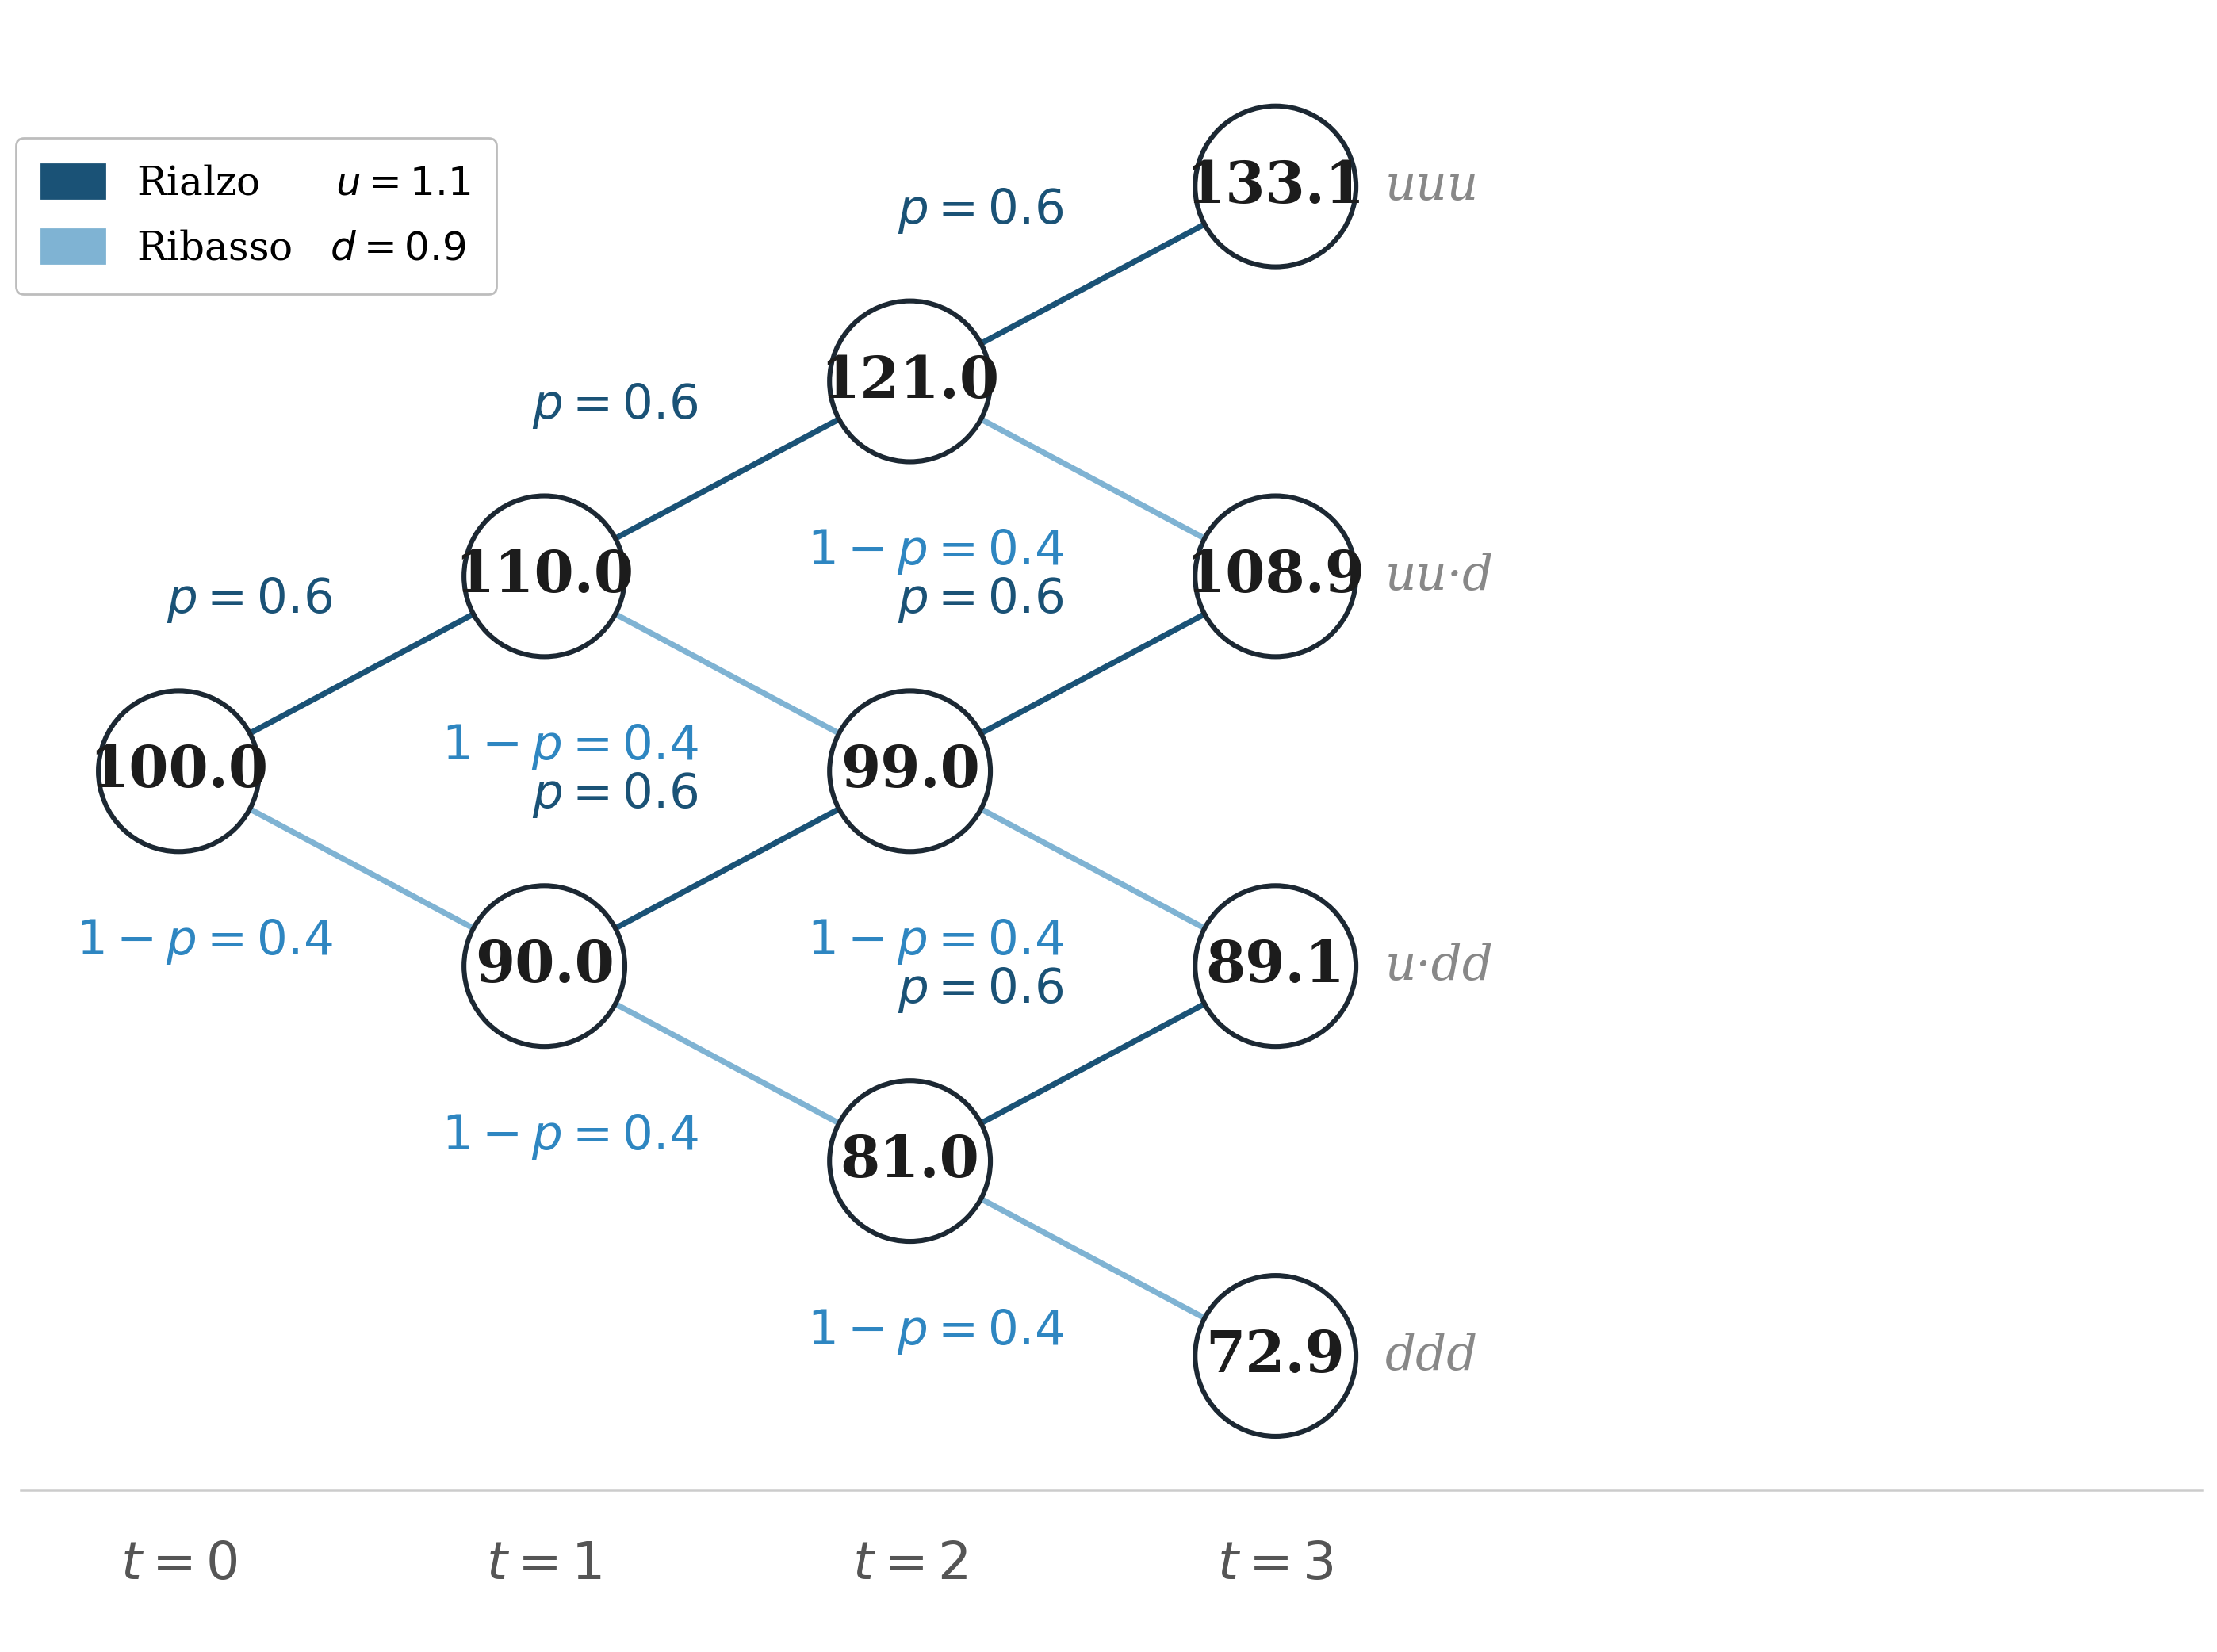
\includegraphics[width=0.92\textwidth]{../graphics/Cap04_Figura_4_1}
\caption{Albero binomiale dei prezzi con $S_0=100$, $u=1.1$,
$d=0.9$, $p=0.6$, $T=3$. Gli archi blu scuro indicano i movimenti
di rialzo (fattore $u$), gli archi azzurri quelli di ribasso
(fattore $d$). I nodi terminali corrispondono agli scenari
$s\in\mathcal{S}=\{1,\ldots,8\}$.}
\label{fig:albero-binomiale}
\end{figure}

La struttura ad albero rende visibili due propriet\`{a} fondamentali.
La prima \`{e} la \emph{non anticipativit\`{a}}: due traiettorie che
coincidono fino al tempo $t$ (cio\`{e} che passano per lo stesso nodo
al tempo $t$) non si distinguono sulla base dell'informazione $\F_t$.
La seconda \`{e} la \emph{ricombinazione}: nel modello binomiale,
poich\`{e} $ud=du$, traiettorie diverse che contengono lo stesso numero
di rialzi e ribassi raggiungono lo stesso nodo. Grazie a questa
propriet\`{a}, il numero di nodi distinti al tempo $t$ \`{e} $t+1$
anzich\`{e} $2^t$: i nodi crescono \emph{linearmente} con $t$, non
esponenzialmente. Per $T=3$ si hanno $4$ nodi terminali anzich\`{e}
$8$ traiettorie distinte, e il numero totale di nodi nell'albero \`{e}
$1+2+3+4=10$ anzich\`{e} $1+2+4+8=15$. Questa compressione \`{e}
computazionalmente cruciale: nei capitoli successivi consente di
calcolare prezzi e valori attesi condizionati su alberi con molti
passi in modo efficiente.

\begin{example}
\label{es:scenari-binomiale}
Per il modello con $S_0=100$, $u=1.1$, $d=0.9$, $p=0.6$, $T=3$, la
Tabella~\ref{tab:scenari-binomiale} elenca gli otto scenari con la
rispettiva probabilit\`{a} e il valore terminale.

\begin{table}[h]
\centering
\begin{tabular}{|c|c|c|c|}
\hline
\textbf{Scenario} $s$ & \textbf{Traiettoria} & $p_s$ & $S_3$\\
\hline
1 & $uuu$ & $0.216$ & $133.1$\\
2 & $uud$ & $0.144$ & $108.9$\\
3 & $udu$ & $0.144$ & $108.9$\\
4 & $duu$ & $0.144$ & $108.9$\\
5 & $udd$ & $0.096$ & $89.1$\\
6 & $dud$ & $0.096$ & $89.1$\\
7 & $ddu$ & $0.096$ & $89.1$\\
8 & $ddd$ & $0.064$ & $72.9$\\
\hline
\multicolumn{2}{|c|}{\textbf{Totale}} & $1.000$ & \\
\hline
\end{tabular}
\caption{Gli otto scenari del processo binomiale con $S_0=100$,
$u=1.1$, $d=0.9$, $p=0.6$, $T=3$.}
\label{tab:scenari-binomiale}
\end{table}
\end{example}


\begin{example}
\label{es:momenti-binomiale}
Per il processo binomiale con $S_0=100$, $u=1.1$, $d=0.9$, $p=0.6$,
$T=3$:
\[
m=0.6\cdot 1.1+0.4\cdot 0.9=1.02,
\qquad
m_2=0.6\cdot 1.21+0.4\cdot 0.81=1.050.
\]
I momenti del processo ai tre orizzonti sono riportati nella
Tabella~\ref{tab:momenti-binomiale}.

\begin{table}[h]
\centering
\begin{tabular}{|c|c|c|c|}
\hline
\textbf{Tempo} $t$ & $\mu(t)=\E[S_t]$ &
$\sigma^2(t)=\Var(S_t)$ & $\sigma(t)$\\
\hline
$0$ & $100.000$ & $0.000$ & $0.000$\\
$1$ & $102.000$ & $104.040$ & $10.200$\\
$2$ & $104.040$ & $215.523$ & $14.681$\\
$3$ & $106.121$ & $334.767$ & $18.297$\\
\hline
\end{tabular}
\caption{Media, varianza e deviazione standard del processo binomiale
($S_0=100$, $u=1.1$, $d=0.9$, $p=0.6$) ai tempi $t=0,1,2,3$. La
deviazione standard cresce con l'orizzonte: l'incertezza sul valore
futuro si accumula nel tempo, coerentemente con la struttura a
incrementi indipendenti.}
\label{tab:momenti-binomiale}
\end{table}

La covarianza tra $S_1$ e $S_3$ \`{e}:
\begin{eqnarray*}
\Cov(S_1,S_3)
&=& S_0^2\bigl(m_2^{\,1}\,m^{\,2}-m^{\,4}\bigr)\\
&=& 10000\,(1.050\cdot 1.0404-1.0824)\\
&=& 99.9,
\end{eqnarray*}
positiva, come atteso: prezzi elevati al tempo 1 tendono ad
accompagnarsi a prezzi elevati al tempo 3.
\end{example}



\subsection{L'incertezza cresce con l'orizzonte}

La Tabella~\ref{tab:momenti-binomiale} mostra che la deviazione
standard $\sigma(t)$ cresce al crescere di $t$. Questo fatto, che
nell'esempio \`{e} verificato numericamente, ha un significato
economico preciso: l'incertezza sul valore futuro di un'attivit\`{a}
finanziaria cresce con l'orizzonte di investimento.

\`{E} possibile quantificare questo effetto in modo esplicito. Per
il modello binomiale con incrementi i.i.d., si dimostra che la
deviazione standard cresce approssimativamente come $\sqrt{t}$ per
$t$ grande. Questo risultato \`{e} coerente con la propriet\`{a}
del moto browniano standard, per cui $\Var(W_t)=t$ e quindi
$\sigma(W_t)=\sqrt{t}$.

\begin{remark}
La crescita dell'incertezza con l'orizzonte ha implicazioni dirette
per la gestione del rischio. Il Value-at-Risk e il CVaR di una
posizione su un orizzonte di $T$ periodi non si ottengono
semplicemente moltiplicando per $T$ le misure di rischio a un
periodo: la struttura temporale della distribuzione delle perdite
deve essere modellata esplicitamente. Questo punto verr\`{a}
ripreso nel Capitolo~7.
\end{remark}


\subsection{Rendimenti logaritmici}

\noindent
\`{E} spesso conveniente descrivere il modello attraverso i
\emph{rendimenti logaritmici} anzich\`{e} i fattori moltiplicativi.
Si definisce
\[
r_t=\log\!\left(\frac{S_t}{S_{t-1}}\right)=\log R_t
\in\{\log u,\;\log d\}.
\]
Nel modello binomiale i rendimenti logaritmici $r_1,\ldots,r_T$ sono
indipendenti e identicamente distribuiti, con
\[
r_t=\begin{cases}
\log u & \text{con probabilit\`{a} }p,\\
\log d & \text{con probabilit\`{a} }1-p.
\end{cases}
\]
Il prezzo si scrive allora come esponenziale di una somma di
rendimenti logaritmici i.i.d.:
\[
S_t=S_0\exp\!\left(\sum_{k=1}^{t}r_k\right).
\]
Il logaritmo del prezzo, $\log S_t=\log S_0+\sum_{k=1}^{t}r_k$,
\`{e} dunque una passeggiata aleatoria nel senso
dell'Esempio~\ref{es:random-walk}. Questa osservazione anticipa il
legame tra il modello binomiale e il moto browniano geometrico: nel
Capitolo~6 vedremo che, facendo tendere a zero l'ampiezza del passo
temporale, la passeggiata aleatoria dei rendimenti logaritmici
converge a un moto browniano, e il modello binomiale dei prezzi al
corrispondente moto browniano geometrico.

\subsection{Sigma-algebra generata da una variabile casuale
e partizione di $\Omega$}

\noindent
Nel Capitolo~3 la sigma-algebra generata da una partizione
$\{B_1,\ldots,B_n\}$ di $\Omega$ era definita come l'insieme di tutti
gli eventi ottenibili come unioni dei blocchi $B_i$. Nella
Sezione~\ref{sec:momenti2} abbiamo introdotto la notazione
$\sigma(X_0,X_1,\ldots,X_t)$: la sigma-algebra \emph{generata da
variabili casuali}. Nel caso del modello binomiale \`{e} importante
verificare esplicitamente che le due notazioni descrivono lo stesso
oggetto, rendendo concreto e calcolabile il concetto generale.

La sigma-algebra $\sigma(X)$ generata da una variabile casuale $X$
che assume un numero finito di valori $v_1,\ldots,v_k$ coincide con
la sigma-algebra generata dalla partizione
\[
\bigl\{\{X=v_1\},\;\ldots,\;\{X=v_k\}\bigr\}.
\]
Conoscere il valore di $X$ equivale dunque a sapere in quale blocco
della partizione si trova l'esito $\omega$. La
Tabella~\ref{tab:sigma-partizione} mostra esplicitamente questa
corrispondenza per la filtrazione naturale del modello binomiale.

\begin{table}[h]
\centering
\begin{tabular}{|p{1.2cm}|p{3.5cm}|p{6.0cm}|}
\hline
\textbf{Tempo} $t$ & \textbf{Sigma-algebra} & \textbf{Partizione
corrispondente di $\Omega$}\\
\hline
$t=0$ & $\F_0=\sigma(S_0)=\{\emptyset,\Omega\}$ &
Unico blocco: \newline $\{uuu,uud,udu,udd,duu,dud,ddu,ddd\}$\\
\hline
$t=1$ & $\F_1=\sigma(S_1)$ &
Due blocchi: \newline $A_u=\{uuu,uud,udu,udd\}$ e \newline
$A_d=\{duu,dud,ddu,ddd\}$\\
\hline
$t=2$ & $\F_2=\sigma(S_1,S_2)$ &
Quattro blocchi: $A_{uu}=\{uuu,uud\}$,
$A_{ud}=\{udu,udd\}$,
$A_{du}=\{duu,dud\}$,
$A_{dd}=\{ddu,ddd\}$\\
\hline
$t=3$ & $\F_3=\sigma(S_1,S_2,S_3)$ &
Otto blocchi: ogni esito elementare forma un blocco
da solo, ad esempio $\{uuu\}$, $\{uud\}$, \ldots,
$\{ddd\}$\\
\hline
\end{tabular}
\caption{Sigma-algebre della filtrazione naturale del processo
binomiale ($S_0=100$, $u=1.1$, $d=0.9$, $T=3$) e partizioni
corrispondenti di $\Omega$. Ogni riga mostra come l'informazione
disponibile al tempo $t$ si traduca in una suddivisione di
$\Omega$ in blocchi indistinguibili sulla base delle osservazioni
fino a $t$.}
\label{tab:sigma-partizione}
\end{table}

\noindent
La tabella chiarisce che la notazione $\sigma(S_1,\ldots,S_t)$ non
aggiunge complessit\`{a} rispetto a quella del Capitolo~3: indica
semplicemente la sigma-algebra generata dalla partizione indotta dai
valori osservati del processo fino al tempo $t$.

\subsection{Filtrazione naturale e processo delle previsioni}

\noindent
La definizione generale di filtrazione naturale \`{e} stata introdotta
nella Sezione~\ref{sec:momenti2}. Nel modello binomiale essa ha una
struttura particolarmente trasparente: al tempo $t=0$ l'unica
informazione disponibile \`{e} quella banale, $\F_0=\{\emptyset,
\Omega\}$; al tempo $t=1$ si sa se il primo movimento \`{e} stato $u$
o $d$, e $\F_1$ distingue i due blocchi $A_u$ e $A_d$; al tempo $t=2$
si conoscono i primi due movimenti e $\F_2$ distingue quattro blocchi;
al tempo $t=3$ l'intera traiettoria \`{e} nota e $\F_3$ distingue
tutti e otto gli esiti.

Su questa filtrazione possiamo costruire concretamente il processo
delle previsioni introdotto in astratto nella
Sezione~\ref{sec:martingale}: la previsione del prezzo terminale
$S_3$ aggiornata all'informazione disponibile a ogni istante.

\begin{example}
\label{es:filtrazione-binomiale}
Nel processo binomiale con $S_0=100$, $u=1.1$, $d=0.9$, $p=0.6$,
$T=3$, calcoliamo il processo delle previsioni
$H_t=\E[S_3\mid\F_t]$ per $t=0,1,2,3$.

\paragraph{Una formula compatta.}
Poich\`{e} $S_3=S_t\cdot R_{t+1}\cdots R_3$ e i fattori futuri sono
indipendenti dall'informazione $\F_t$, con $\E[R_k]=m=1.02$:
\[
H_t=\E[S_3\mid\F_t]
=S_t\,\E[R_{t+1}\cdots R_3\mid\F_t]
=S_t\,m^{\,3-t}.
\]
La previsione del prezzo terminale \`{e} dunque il prezzo corrente
$S_t$ capitalizzato al rendimento medio $m$ per i periodi residui.

\paragraph{Calcolo nei due nodi al tempo $t=1$.}
Al tempo $t=1$ la filtrazione distingue il nodo $A_u$ (prezzo corrente
$S_1=110$) e il nodo $A_d$ ($S_1=90$). Verifichiamo la formula
compatta tramite il calcolo diretto. Per $\omega\in A_u$ i tre valori
terminali raggiungibili sono
\[
S_3=\begin{cases}
u^2\cdot 110=133.1 & \text{con probabilit\`{a} }p^2=0.36,\\
ud\cdot 110=108.9 & \text{con probabilit\`{a} }2p(1-p)=0.48,\\
d^2\cdot 110=89.1 & \text{con probabilit\`{a} }(1-p)^2=0.16,
\end{cases}
\]
da cui
\[
\E[S_3\mid A_u]=133.1\cdot 0.36+108.9\cdot 0.48+89.1\cdot 0.16
=114.444,
\]
in accordo con $S_1\,m^2=110\cdot 1.0404=114.444$. Analogamente, per
$\omega\in A_d$:
\[
\E[S_3\mid A_d]=108.9\cdot 0.36+89.1\cdot 0.48+72.9\cdot 0.16
=93.636=90\cdot 1.0404.
\]

\paragraph{Il processo delle previsioni sull'albero.}
Applicando la formula $H_t=S_t\,m^{\,3-t}$ a tutti i nodi si ottiene
il processo delle previsioni completo, riportato nella
Tabella~\ref{tab:previsioni-binomiale}.

\begin{table}[h]
\centering
\begin{tabular}{|c|l|}
\hline
\textbf{Tempo} $t$ & \textbf{Valori di } $H_t=\E[S_3\mid\F_t]$
\textbf{ nei nodi}\\
\hline
$0$ & $106.121$\\
$1$ & $114.444$ (nodo $u$), \quad $93.636$ (nodo $d$)\\
$2$ & $123.420$ (uu), \quad $100.980$ (ud), \quad $82.620$ (dd)\\
$3$ & $133.100$ (uuu), \quad $108.900$ (uud), \quad
       $89.100$ (udd), \quad $72.900$ (ddd)\\
\hline
\end{tabular}
\caption{Il processo delle previsioni $H_t=\E[S_3\mid\F_t]=S_t\,
m^{\,3-t}$ in tutti i nodi dell'albero binomiale. Al tempo $t=3$ la
previsione coincide con il valore realizzato $S_3$; al tempo $t=0$
coincide con la media incondizionata $\E[S_3]=106.121$.}
\label{tab:previsioni-binomiale}
\end{table}

\paragraph{Il processo delle previsioni \`{e} una martingala.}
Il processo $\{H_t\}$ \`{e} una martingala rispetto a $\{\F_t\}$, in
accordo con il risultato generale sulla martingala di Doob
(Sezione~\ref{sec:martingale}). Verifichiamolo su un passo, dal nodo
$u$ al tempo $1$ ai suoi due successori al tempo $2$ (i nodi uu e ud):
\[
\E[H_2\mid A_u]=0.6\cdot 123.420+0.4\cdot 100.980
=74.052+40.392=114.444=H_1(A_u).
\]
La previsione fatta oggi della previsione di domani coincide con la
previsione di oggi: le revisioni della previsione non sono prevedibili
in anticipo. In particolare, prendendo il valore atteso dal tempo $1$
al tempo $0$ si ritrova la propriet\`{a} della torre:
\[
\E[H_1]=0.6\cdot 114.444+0.4\cdot 93.636=106.121=\E[S_3].
\]

\paragraph{Attenzione: il processo dei prezzi non \`{e} una
martingala.} \`{E} importante non confondere il processo delle
previsioni $\{H_t\}$ con il processo dei prezzi $\{S_t\}$. Il primo
\`{e} sempre una martingala. Il secondo lo \`{e} solo se il rendimento
medio per periodo \`{e} unitario, $m=1$. Nel nostro esempio $m=1.02>1$,
e infatti
\[
\E[S_1\mid\F_0]=0.6\cdot 110+0.4\cdot 90=102=S_0\,m>S_0:
\]
il processo dei prezzi \`{e} una submartingala, coerentemente con il
fatto che un investimento azionario ha rendimento atteso positivo. La
condizione $m=1$, sotto la quale il prezzo diventa una martingala, ha
un ruolo centrale nella valutazione risk-neutral, che riprenderemo nei
capitoli dedicati al pricing.
\end{example}

% ============================================================
% MQF_Cap_05_Sezione_5_7.tex
% Capitolo 5 - Sezione 5.7
% Simulazione: logica generale e stima Monte Carlo
%
% Sezione nuova. Resta a livello generale (tempo discreto):
% niente modelli continui specifici ne' Eulero-Maruyama,
% che arrivano nel Capitolo 6.
% ============================================================

\section{Simulazione: logica generale e stima Monte Carlo}
\label{sec:simulazione}

\noindent
Molte quantit\`{a} di interesse in finanza --- il prezzo atteso di un
contratto, la perdita attesa di un portafoglio, la probabilit\`{a} di
superare una soglia di rischio --- si esprimono come valori attesi di
funzioni di un processo stocastico. In casi semplici, come il modello
binomiale della Sezione~\ref{sec:binomiale}, questi valori attesi si
calcolano in forma chiusa sommando su tutti gli scenari. Ma non appena
il numero di periodi cresce, o la dinamica del processo si fa pi\`{u}
complessa, l'enumerazione esplicita di tutti gli scenari diventa
impraticabile: un albero binomiale con $T=50$ periodi ha gi\`{a}
$2^{50}$ traiettorie, oltre mille miliardi. In questi casi si ricorre
alla \emph{simulazione}.

L'idea della simulazione \`{e} semplice e potente: invece di enumerare
tutti gli scenari possibili, se ne generano molti \emph{a caso},
coerentemente con la legge del processo, e si stima la quantit\`{a} di
interesse come media empirica sui soli scenari generati. Questa
sezione ne presenta la logica in forma generale, valida per qualunque
processo a tempo discreto. La sua applicazione ai modelli in tempo
continuo, mediante la discretizzazione delle equazioni differenziali
stocastiche, sar\`{a} sviluppata nel Capitolo~6 e implementata in
Python nella lezione applicativa.

\subsection{Generazione di traiettorie}

\noindent
Simulare un processo $\{X_t\}_{t=0}^{T}$ significa generare una
\emph{replica} della sua traiettoria, ovvero una sequenza di valori
$X_0^{(k)},X_1^{(k)},\ldots,X_T^{(k)}$ che costituisce una possibile
realizzazione del processo. Generando $M$ repliche indipendenti
\[
\bigl\{X_0^{(k)},X_1^{(k)},\ldots,X_T^{(k)}\bigr\},
\qquad k=1,2,\ldots,M,
\]
si ottiene un campione di $M$ traiettorie, ciascuna corrispondente a
un possibile percorso del processo.

Per un processo definito da una dinamica ricorsiva --- come il modello
binomiale, in cui $X_{t+1}$ si ottiene da $X_t$ applicando un
movimento aleatorio --- la generazione di una traiettoria procede in
modo sequenziale: si parte dal valore iniziale $X_0$, noto, e a ogni
passo si estrae l'innovazione casuale (nel caso binomiale, il
movimento $u$ o $d$) e si calcola il valore successivo. Ripetendo la
procedura per $T$ passi si ottiene un'intera traiettoria; ripetendola
per $M$ repliche indipendenti si ottiene il campione.

\begin{remark}
La fedelt\`{a} della simulazione dipende interamente dalla qualit\`{a}
del generatore di numeri casuali utilizzato per estrarre le
innovazioni. I generatori impiegati nella pratica sono in realt\`{a}
\emph{pseudo-casuali}: producono sequenze deterministiche che
imitano le propriet\`{a} statistiche dell'aleatoriet\`{a}. Questo ha
un risvolto utile: fissando il \emph{seme} (seed) del generatore, una
simulazione diventa esattamente riproducibile, il che \`{e}
essenziale per il controllo e la validazione dei risultati. Questo
aspetto operativo sar\`{a} ripreso nella lezione in Python.
\end{remark}

\subsection{La stima Monte Carlo}

\noindent
Supponiamo di voler calcolare il valore atteso $\E[g(X_T)]$ di una
funzione del processo --- ad esempio $g(X_T)=X_T$ per il valore atteso
terminale, oppure $g(X_T)=\max(X_T-K,0)$ per il payoff di un'opzione
call con prezzo di esercizio $K$. La \emph{stima Monte Carlo} di
questo valore atteso \`{e} la media empirica della funzione sulle $M$
traiettorie simulate:
\[
\widehat{\theta}_M=\frac{1}{M}\sum_{k=1}^{M}g\bigl(X_T^{(k)}\bigr).
\]
La giustificazione teorica di questa stima \`{e} la legge dei grandi
numeri, gi\`{a} incontrata nel Capitolo~2: poich\`{e} le repliche sono
indipendenti e identicamente distribuite, la media empirica converge
al valore atteso vero al crescere del numero di repliche,
\[
\widehat{\theta}_M\xrightarrow[M\to\infty]{}\theta=\E[g(X_T)].
\]
La simulazione Monte Carlo trasforma dunque il calcolo di un valore
atteso --- operazione che richiederebbe la conoscenza dell'intera
distribuzione di $g(X_T)$ --- in un semplice problema di media
campionaria, al prezzo di un errore di stima che, come vedremo,
si pu\`{o} controllare.

La stessa logica si applica a quantit\`{a} condizionate. La media di
$g(X_T)$ ristretta agli scenari che soddisfano una certa condizione
$A$ --- ad esempio gli scenari in cui il processo non scende mai sotto
una soglia --- si stima con
\[
\widehat{\theta}_M^{\,A}
=\frac{1}{M_A}\sum_{k:\,\omega^{(k)}\in A}g\bigl(X_T^{(k)}\bigr),
\qquad
M_A=\#\{k:\omega^{(k)}\in A\},
\]
ovvero come media della funzione sui soli scenari che ricadono in $A$,
dove $M_A$ \`{e} il numero di tali scenari.

\begin{example}[Stima del prezzo atteso terminale]
\label{es:montecarlo-binomiale}
Si consideri il modello binomiale con $S_0=100$, $u=1.1$, $d=0.9$,
$p=0.6$, $T=3$. Il valore atteso terminale esatto, calcolato nella
Sezione~\ref{sec:binomiale}, \`{e} $\E[S_3]=106.121$. Una simulazione
Monte Carlo lo stima generando $M$ traiettorie e mediando i valori
terminali $S_3^{(k)}$. Al crescere di $M$, la stima
$\widehat{\theta}_M$ si avvicina al valore esatto: con poche centinaia
di repliche l'approssimazione \`{e} gi\`{a} ragionevole, con alcune
decine di migliaia diventa accurata alle prime cifre decimali. In un
modello cos\`{\i} semplice la simulazione non \`{e} necessaria, poich\`{e}
il valore esatto \`{e} noto; ma essa fornisce un banco di prova ideale,
perch\`{e} permette di confrontare la stima simulata con il risultato
analitico e di verificare cos\`{\i} la correttezza della procedura ---
un passo di validazione che riprenderemo in Python.
\end{example}

\subsection{L'incertezza della stima}

\noindent
La stima Monte Carlo \`{e} essa stessa una quantit\`{a} aleatoria:
ripetendo l'intera simulazione con un diverso insieme di numeri
casuali si otterrebbe un valore leggermente diverso. \`{E} dunque
essenziale accompagnare la stima con una misura della sua incertezza.

Indichiamo con $\sigma_g^2=\Var\bigl(g(X_T)\bigr)$ la varianza della
quantit\`{a} simulata su una singola replica. Poich\`{e} la stima
$\widehat{\theta}_M$ \`{e} la media di $M$ repliche indipendenti, la
sua varianza \`{e}
\[
\Var\bigl(\widehat{\theta}_M\bigr)=\frac{\sigma_g^2}{M},
\]
e la sua deviazione standard --- detta \emph{errore standard} della
stima --- \`{e}
\[
\operatorname{SE}\bigl(\widehat{\theta}_M\bigr)
=\frac{\sigma_g}{\sqrt{M}}.
\]
Nella pratica $\sigma_g$ non \`{e} noto e si stima a sua volta dalla
deviazione standard campionaria delle repliche.

Questa formula racchiude la propriet\`{a} fondamentale --- e il limite
principale --- del metodo Monte Carlo: l'errore di stima decresce come
$1/\sqrt{M}$. Per dimezzare l'errore standard occorre quadruplicare il
numero di repliche; per guadagnare una cifra decimale di precisione
occorre moltiplicare per cento il numero di simulazioni. Questa
convergenza lenta \`{e} il prezzo della generalit\`{a} del metodo, ed
\`{e} la ragione per cui esistono numerose tecniche di
\emph{riduzione della varianza}, volte a diminuire $\sigma_g$ a
parit\`{a} di $M$, che la lezione in Python avr\`{a} modo di
illustrare.

\begin{remark}
Il fatto che l'errore decresca come $1/\sqrt{M}$, indipendentemente
dal numero di periodi $T$ o dalla complessit\`{a} del processo, \`{e}
ci\`{o} che rende la simulazione Monte Carlo cos\`{\i} preziosa nelle
applicazioni finanziarie. Mentre l'enumerazione esplicita degli
scenari ha un costo che cresce esponenzialmente con $T$, il costo
della simulazione cresce solo linearmente con $M$ e con $T$. \`{E}
per questo che la simulazione diventa il metodo di elezione non
appena la dimensione del problema supera la soglia in cui i metodi
esatti restano praticabili --- una situazione tipica nei modelli in
tempo continuo del prossimo capitolo, dove ogni traiettoria \`{e}
ottenuta discretizzando un'equazione differenziale stocastica su una
griglia temporale fitta.
\end{remark}

% ============================================================
% MQF_Cap_05_Sezione_5_8.tex
% Capitolo 5 - Sezione 5.8
% Esercizi svolti
%
% Formato soluzioni: \textbf{Soluzione.} + itemize
% (non si usa l'ambiente solution)
% ============================================================

\section{Esercizi svolti}
\label{sec:esercizi-svolti}

\begin{exercise}[Profitto cumulato di un desk di trading]
\label{ex:random-walk}
Un desk di trading realizza ogni giorno un profitto $Z_k$ che,
in migliaia di euro, assume due valori:
\[
Z_k=\begin{cases}
+3 & \text{con probabilit\`{a} }0.5,\\
-1 & \text{con probabilit\`{a} }0.5,
\end{cases}
\]
con i diversi giorni indipendenti e identicamente distribuiti. Il
profitto cumulato dopo $t$ giorni \`{e} $X_t=\sum_{k=1}^{t}Z_k$, con
$X_0=0$.
\begin{enumerate}
\item Calcolare media e varianza del profitto giornaliero (uguali per
ogni giorno, essendo le $Z_k$ i.i.d.).
\item Determinare le funzioni $\mu(t)=\E[X_t]$ e
$\sigma^2(t)=\Var(X_t)$.
\item Calcolare $\Cov(X_2,X_5)$.
\item Stabilire se $\{X_t\}$ \`{e} una martingala, una submartingala
o una supermartingala rispetto alla propria filtrazione naturale.
\end{enumerate}
\end{exercise}

\noindent
\textbf{Soluzione.}
\begin{enumerate}
\item Poich\'{e} le variabili $Z_1,Z_2,\ldots$ sono identicamente
distribuite, media e varianza non dipendono dall'indice: il calcolo
svolto per un generico tempo $k$ vale per ogni giorno. Per ogni
$k\geq 1$,
\[
\nu=\E[Z_k]=0.5\cdot 3+0.5\cdot(-1)=1.
\]
Per la varianza, sempre per ogni $k\geq 1$,
\[
\E[Z_k^2]=0.5\cdot 9+0.5\cdot 1=5,
\qquad
\tau^2=\Var(Z_k)=\E[Z_k^2]-\nu^2=5-1=4.
\]

\item Trattandosi di una passeggiata aleatoria con incrementi
i.i.d., per i risultati della Sezione~\ref{sec:momenti2}:
\[
\mu(t)=t\,\nu=t,
\qquad
\sigma^2(t)=t\,\tau^2=4t.
\]
La deviazione standard $\sigma(t)=2\sqrt{t}$ cresce con la radice
dell'orizzonte: l'incertezza sul profitto cumulato si accumula nel
tempo.

\item Per la struttura di covarianza della passeggiata aleatoria, con
$s\leq t$ vale $c(s,t)=\min(s,t)\,\tau^2$. Quindi
\[
\Cov(X_2,X_5)=\min(2,5)\cdot 4=2\cdot 4=8.
\]

\item Per $s\leq t$:
\[
\E[X_t\mid\F_s]=X_s+(t-s)\,\nu=X_s+(t-s)\geq X_s,
\]
con disuguaglianza stretta per $t>s$. Il processo \`{e} dunque una
\emph{submartingala}: il desk ha un vantaggio sistematico
($\nu=1>0$), e il profitto cumulato tende a crescere in media. Solo
se il profitto medio giornaliero fosse nullo il processo sarebbe una
martingala.
\end{enumerate}

\begin{exercise}[Albero binomiale a due periodi]
\label{ex:binomiale}
Un'azione vale oggi $S_0=80$. A ogni periodo il prezzo sale del
$25\%$ (fattore $u=1.25$) con probabilit\`{a} $p=0.5$, oppure scende
del $20\%$ (fattore $d=0.8$) con probabilit\`{a} $1-p=0.5$. Si
considera l'orizzonte $T=2$.
\begin{enumerate}
\item Costruire l'albero dei prezzi ed elencare gli scenari con le
rispettive probabilit\`{a}.
\item Calcolare $\E[S_2]$ e verificarlo con la formula
$\E[S_2]=S_0\,m^2$.
\item Calcolare $\E[S_2\mid\F_1]$ nei due nodi al tempo $1$ e
verificare la propriet\`{a} della torre.
\end{enumerate}
\end{exercise}

\noindent
\textbf{Soluzione.}
\begin{enumerate}

\item Il rendimento lordo medio per periodo \`{e}
\[
m=pu+(1-p)d=0.5\cdot 1.25+0.5\cdot 0.8=1.025.
\]
I valori del prezzo nei nodi sono:
\[
\begin{array}{ll}
t=0: & S_0=80;\\
t=1: & S_1^u=80\cdot 1.25=100, \quad S_1^d=80\cdot 0.8=64;\\
t=2: & S_2^{uu}=125, \quad S_2^{ud}=S_2^{du}=80,
       \quad S_2^{dd}=51.2.
\end{array}
\]
I quattro scenari, con probabilit\`{a} $p_s=0.25$ ciascuno (essendo
$p=0.5$), sono: $uu$ con $S_2=125$; $ud$ e $du$ con $S_2=80$; $dd$ con
$S_2=51.2$.

\item Sommando sugli scenari:
\[
\E[S_2]=0.25\cdot 125+0.5\cdot 80+0.25\cdot 51.2
=31.25+40+12.8=84.05.
\]
La formula compatta conferma: $\E[S_2]=S_0\,m^2=80\cdot
1.025^2=80\cdot 1.050625=84.05$.

\item Al nodo $u$ ($S_1=100$), i due esiti al tempo $2$ sono $125$ e
$80$, ciascuno con probabilit\`{a} $0.5$:
\[
\E[S_2\mid A_u]=0.5\cdot 125+0.5\cdot 80=102.5=100\cdot 1.025.
\]
Al nodo $d$ ($S_1=64$), gli esiti sono $80$ e $51.2$:
\[
\E[S_2\mid A_d]=0.5\cdot 80+0.5\cdot 51.2=65.6=64\cdot 1.025.
\]
Verifica della torre:
\[
\E\bigl[\E[S_2\mid\F_1]\bigr]
=0.5\cdot 102.5+0.5\cdot 65.6=51.25+32.8=84.05=\E[S_2].
\]
\end{enumerate}

\begin{exercise}[Prezzo scontato e misura di martingala]
\label{ex:scontato}
Si consideri un periodo singolo. Un'azione vale $S_0=100$ e tra un
periodo varr\`{a} $S_1=120$ (rialzo) oppure $S_1=90$ (ribasso). Il
tasso privo di rischio per il periodo \`{e} $r=0.05$. Si definisca la
probabilit\`{a} di rialzo $q$ in modo che il prezzo scontato
$\tilde{S}_t=S_t/(1+r)^t$ sia una martingala, cio\`{e} tale che
$\E_{\Q}[\tilde{S}_1]=\tilde{S}_0=S_0$.
\begin{enumerate}
\item Determinare il valore di $q$.
\item Verificare che, sotto tale probabilit\`{a}, il prezzo scontato
soddisfa la propriet\`{a} di martingala.
\item Interpretare il risultato.
\end{enumerate}
\end{exercise}

\noindent
\textbf{Soluzione.}
\begin{enumerate}
\item La condizione di martingala per il prezzo scontato su un periodo
\`{e}
\[
\frac{1}{1+r}\,\E_{\Q}[S_1]=S_0,
\qquad\text{ossia}\qquad
\E_{\Q}[S_1]=S_0(1+r).
\]
Con $\E_{\Q}[S_1]=q\cdot 120+(1-q)\cdot 90$ e $S_0(1+r)=105$:
\[
120q+90(1-q)=105
\;\Longrightarrow\;
30q=15
\;\Longrightarrow\;
q=0.5.
\]
In generale $q=\dfrac{(1+r)S_0-S_1^d}{S_1^u-S_1^d}
=\dfrac{105-90}{120-90}=0.5$, formula che riprenderemo nei capitoli
sul pricing.

\item Sotto $\Q$ con $q=0.5$:
\[
\E_{\Q}[\tilde{S}_1]
=\frac{1}{1.05}\bigl(0.5\cdot 120+0.5\cdot 90\bigr)
=\frac{105}{1.05}=100=\tilde{S}_0.
\]
Il prezzo scontato \`{e} dunque una martingala sotto $\Q$.

\item La probabilit\`{a} $q=0.5$ non \`{e} la probabilit\`{a}
\emph{fisica} con cui il mercato sale o scende, ma una probabilit\`{a}
\emph{artificiale} --- la misura risk-neutral $\Q$ --- costruita in
modo che il prezzo scontato dell'azione diventi una martingala. Sotto
questa misura, ogni attivit\`{a} ha rendimento atteso pari al tasso
privo di rischio. \`{E} questa la propriet\`{a} che, nei capitoli sul
pricing, consentir\`{a} di valutare un derivato come valore atteso
scontato del suo payoff sotto $\Q$.
\end{enumerate}

\begin{exercise}[Dimensionamento di una simulazione Monte Carlo]
\label{ex:montecarlo}
Si vuole stimare per simulazione il prezzo atteso $\theta=\E[g(X_T)]$
di un contratto. Una simulazione pilota con $M_0=1\,000$ repliche
fornisce una stima $\widehat{\theta}=12.4$ e una deviazione standard
campionaria delle repliche pari a $s_g=15$.
\begin{enumerate}
\item Stimare l'errore standard della stima pilota e costruire un
intervallo di confidenza approssimato al $95\%$ per $\theta$.
\item Determinare il numero di repliche necessario affinch\'{e}
l'errore standard scenda a $0.05$.
\end{enumerate}
\end{exercise}

\noindent
\textbf{Soluzione.}
\begin{enumerate}
\item L'errore standard della stima pilota \`{e}
\[
\operatorname{SE}=\frac{s_g}{\sqrt{M_0}}
=\frac{15}{\sqrt{1\,000}}
=\frac{15}{31.62}\approx 0.474.
\]
Un intervallo di confidenza approssimato al $95\%$, usando il
quantile $1.96$ della normale standard, \`{e}
\[
\widehat{\theta}\pm 1.96\cdot\operatorname{SE}
=12.4\pm 1.96\cdot 0.474
=12.4\pm 0.93,
\]
ossia all'incirca l'intervallo $[11.47,\;13.33]$.

\item Imponendo $\operatorname{SE}=s_g/\sqrt{M}\leq 0.05$ e
risolvendo per $M$:
\[
\sqrt{M}\geq\frac{s_g}{0.05}=\frac{15}{0.05}=300
\;\Longrightarrow\;
M\geq 300^2=90\,000.
\]
Per ridurre l'errore standard da $0.474$ a $0.05$, ovvero di un
fattore circa $9.5$, occorre aumentare il numero di repliche di un
fattore $9.5^2\approx 90$: dalle mille repliche iniziali a circa
novantamila. Questo illustra concretamente la convergenza $1/\sqrt{M}$
del metodo Monte Carlo, e il motivo per cui, quando l'accuratezza
richiesta \`{e} elevata, diventano interessanti le tecniche di
riduzione della varianza.
\end{enumerate}

% ============================================================
% MQF_Cap_05_Sezione_5_9.tex
% Capitolo 5 - Sezione 5.9
% Esercizi proposti
%
% Sei esercizi di difficolta' crescente. Per ciascuno e' indicato
% il solo risultato finale, per l'autovalutazione (puo' essere
% rimosso se si preferisce non fornirlo).
% ============================================================

\section{Esercizi proposti}
\label{sec:esercizi-proposti}

\begin{exercise}[Posizione di cassa aleatoria]
\label{ex:prop-rw}
La posizione di cassa giornaliera di un'attivit\`{a} varia ogni giorno
di una quantit\`{a} $Z_k$ che vale $+2$ con probabilit\`{a} $0.6$ e
$-2$ con probabilit\`{a} $0.4$ (in migliaia di euro), con giorni
indipendenti. Sia $X_t=\sum_{k=1}^{t}Z_k$ la posizione cumulata,
$X_0=0$.
\begin{enumerate}
\item Calcolare media e varianza di $Z_k$.
\item Determinare $\mu(t)$ e $\sigma(t)$, e calcolare i loro valori
per $t=10$.
\item Stabilire se $\{X_t\}$ \`{e} martingala, submartingala o
supermartingala.
\end{enumerate}
\textit{Risultati:} $\nu=0.4$, $\tau^2=3.84$; $\mu(10)=4$,
$\sigma(10)\approx 6.20$; submartingala.
\end{exercise}

\begin{exercise}[Albero binomiale a tre periodi]
\label{ex:prop-binomiale}
Un'azione vale $S_0=50$. A ogni periodo sale del $20\%$ ($u=1.2$) con
probabilit\`{a} $p=0.55$, oppure scende del $10\%$ ($d=0.9$) con
probabilit\`{a} $0.45$. Si consideri $T=3$.
\begin{enumerate}
\item Determinare i quattro valori terminali distinti di $S_3$ e le
loro probabilit\`{a}.
\item Calcolare $\E[S_3]$, sia sommando sugli scenari sia con la
formula $S_0\,m^3$.
\item Calcolare la deviazione standard $\sigma(3)$.
\end{enumerate}
\textit{Risultati:} $m=1.065$; valori terminali $86.40$, $64.80$,
$48.60$, $36.45$; $\E[S_3]\approx 60.40$.
\end{exercise}

\begin{exercise}[Processi adattati e anticipativi]
\label{ex:prop-adattato}
Sia $\{S_t\}_{t=0}^{T}$ un processo dei prezzi con filtrazione
naturale $\{\F_t\}$. Per ciascuno dei seguenti processi, stabilire se
\`{e} adattato o anticipativo rispetto a $\{\F_t\}$, motivando la
risposta:
\begin{enumerate}
\item $Y_t=\tfrac{1}{2}(S_t+S_{t-1})$, la media tra prezzo corrente e
prezzo del periodo precedente;
\item $Y_t=S_{t+1}-S_t$, la variazione del periodo successivo;
\item $Y_t=\min_{0\leq s\leq t}S_s$, il prezzo minimo osservato fino
a $t$;
\item $Y_t=\E[S_T\mid\F_t]$, la previsione del prezzo terminale.
\end{enumerate}
\textit{Risultati:} adattati i processi (1), (3) e (4); anticipativo
il processo (2).
\end{exercise}

\begin{exercise}[Processo delle previsioni e torre]
\label{ex:prop-previsioni}
Si riprenda l'azione dell'Esercizio~\ref{ex:prop-binomiale}
($S_0=50$, $u=1.2$, $d=0.9$, $p=0.55$, $T=3$). Si consideri il
processo delle previsioni $H_t=\E[S_3\mid\F_t]$.
\begin{enumerate}
\item Usando la formula compatta $H_t=S_t\,m^{\,3-t}$, calcolare il
valore di $H_2$ nei tre nodi al tempo $t=2$.
\item Verificare la propriet\`{a} di martingala passando dal nodo
$uu$ al tempo $2$ ai suoi successori al tempo $3$.
\end{enumerate}
\textit{Risultati:} $S_2$ nei tre nodi $=72$, $54$, $40.5$; quindi
$H_2=76.68$, $57.51$, $43.13$.
\end{exercise}

\begin{exercise}[Condizione di martingala per i prezzi]
\label{ex:prop-martingala}
In un modello binomiale i fattori sono $u=1.1$ e $d=0.95$. Si
determini la probabilit\`{a} di rialzo $p$ che rende il processo dei
prezzi $\{S_t\}$ una martingala rispetto alla propria filtrazione
naturale. Interpretare il risultato confrontandolo con il rendimento
atteso di un investimento azionario reale.

\smallskip
\textit{Risultato:} la condizione \`{e} $m=pu+(1-p)d=1$, da cui
$p=1/3$. Poich\'{e} un'azione reale ha rendimento atteso positivo
($m>1$), la probabilit\`{a} fisica \`{e} in genere maggiore di $1/3$:
il prezzo \`{e} una submartingala sotto la misura fisica.
\end{exercise}

\begin{exercise}[Precisione di una stima Monte Carlo]
\label{ex:prop-montecarlo}
Per stimare il prezzo atteso di un contratto si esegue una simulazione
con $M=2\,500$ repliche, ottenendo una stima $\widehat{\theta}=18.7$
e una deviazione standard campionaria $s_g=8$.
\begin{enumerate}
\item Calcolare l'errore standard della stima e un intervallo di
confidenza approssimato al $95\%$.
\item Determinare il numero di repliche necessario per portare
l'errore standard a $0.02$.
\end{enumerate}
\textit{Risultati:} $\operatorname{SE}=0.16$, intervallo
$18.7\pm 0.314$; servono $M=160\,000$ repliche.
\end{exercise}

% ============================================================
% MQF_Cap_05_Sezione_5_10.tex
% Capitolo 5 - Sezione 5.10
% Sintesi e ponte verso il Capitolo 6
%
% NOTA: la sintesi NON cita i casi d'uso specifici del Cap. 6
% (opzioni asiatiche, OU, CIR, obbligazioni indicizzate).
% ============================================================

\section{Sintesi}
\label{sec:sintesi-cap5}

\noindent
Questo capitolo ha introdotto il linguaggio dei processi stocastici e
gli strumenti per descriverne il comportamento nel tempo. Conviene
ripercorrere i concetti principali, raggruppati per funzione, prima di
indicare come essi verranno utilizzati nel seguito del corso.

\subsection{I concetti fondamentali}

\noindent
Il capitolo si \`{e} sviluppato lungo tre direttrici.

\paragraph{1. La descrizione di un processo.}
Un processo stocastico $\{X_t\}_{t\in\mathcal{T}}$ \`{e} una famiglia
di variabili casuali indicizzata dal tempo, leggibile a tre livelli:
la distribuzione marginale a un istante fissato, la traiettoria per un
esito fissato, la famiglia nel suo complesso. La sua struttura
temporale si descrive sinteticamente mediante la funzione media
$\mu(t)$, la funzione varianza $\sigma^2(t)$ e la funzione di
autocovarianza $c(s,t)$, e si caratterizza attraverso le propriet\`{a}
degli incrementi --- indipendenza e stazionariet\`{a} --- e le
nozioni di stazionariet\`{a} del processo.

\paragraph{2. L'informazione e la sua evoluzione.}
Il flusso progressivo dell'informazione si formalizza mediante una
filtrazione $\{\F_t\}$, successione crescente di sigma-algebre. Un
processo \`{e} adattato se il suo valore a ogni istante \`{e}
osservabile con l'informazione disponibile in quell'istante; \`{e}
anticipativo in caso contrario. Solo i processi adattati descrivono
quantit\`{a} e strategie effettivamente implementabili.

\paragraph{3. Le martingale.}
Una martingala formalizza l'idea di gioco equo: la migliore previsione
del valore futuro coincide con il valore presente. Submartingale e
supermartingale descrivono giochi rispettivamente favorevoli e
sfavorevoli. Il processo delle previsioni di una qualunque quantit\`{a}
terminale \`{e} sempre una martingala, e la propriet\`{a} di martingala
del prezzo scontato, sotto un'opportuna misura, \`{e} il fondamento
della valutazione dei derivati.

La Tabella~\ref{tab:sintesi-cap5} raccoglie questi concetti con la
notazione introdotta e il loro significato.

\begin{table}[h]
\centering
\begin{tabular}{|p{2.5cm}|p{3.8cm}|p{4.5cm}|}
\hline
\textbf{Concetto} & \textbf{Notazione} & \textbf{Significato}\\
\hline
Processo stocastico & $\{X_t\}_{t\in\mathcal{T}}$ &
Famiglia di variabili casuali indicizzata dal tempo\\
\hline
Traiettoria & $t\mapsto X_t(\omega)$ &
Realizzazione del processo per un esito fissato\\
\hline
Funzione media & $\mu(t)=\E[X_t]$ &
Livello medio del processo nel tempo\\
\hline
Autocovarianza & $c(s,t)=\Cov(X_s,X_t)$ &
Dipendenza lineare tra istanti diversi\\
\hline
Filtrazione & $\{\F_t\}$ &
Flusso crescente dell'informazione\\
\hline
Processo adattato & $X_t$ $\F_t$-misurabile &
Quantit\`{a} osservabile al tempo $t$\\
\hline
Martingala & $\E[X_t\mid\F_s]=X_s$ &
Gioco equo; previsione $=$ valore presente\\
\hline
Scenario & $s\in\mathcal{S}$, $p_s$, $\xi_s$ &
Traiettoria discreta con la sua probabilit\`{a}\\
\hline
Stima Monte Carlo &
$\widehat{\theta}_M=\frac{1}{M}\sum_k g(X_T^{(k)})$ &
Media empirica su $M$ traiettorie simulate\\
\hline
\end{tabular}
\caption{Sintesi dei concetti del Capitolo~5.}
\label{tab:sintesi-cap5}
\end{table}

\subsection{Il modello binomiale come palestra}

\noindent
Tutti questi concetti, introdotti in forma generale, sono stati
applicati a un modello concreto --- il modello binomiale dei prezzi
--- scelto per la possibilit\`{a} di svolgere ogni calcolo
esplicitamente e di visualizzare la struttura del processo mediante
l'albero degli scenari. Su questo modello abbiamo calcolato momenti,
costruito la filtrazione naturale, verificato la propriet\`{a} della
torre e illustrato il processo delle previsioni come martingala. Il
modello binomiale ha cos\`{\i} svolto la funzione di banco di prova
dei concetti generali, su un caso in cui ogni risultato pu\`{o} essere
controllato a mano.

\subsection{Verso i modelli in tempo continuo}

\noindent
Gli strumenti sviluppati in questo capitolo --- processo, traiettoria,
momenti, filtrazione, martingala, scenario, simulazione --- non sono
legati al tempo discreto: sono stati definiti in modo da valere per
qualunque insieme di indici temporali. Il capitolo successivo li
applicher\`{a} ai \emph{processi in tempo continuo}, in cui il tempo
varia con continuit\`{a} e le traiettorie diventano funzioni definite
su un intervallo.

Il passaggio al tempo continuo non \`{e} un mero raffinamento tecnico.
\`{E} il linguaggio in cui sono formulati i principali modelli per i
prezzi delle attivit\`{a}, per i tassi di interesse e per i fattori di
rischio, ed \`{e} il contesto naturale per le applicazioni di
simulazione e valutazione che costituiscono il cuore operativo della
parte successiva del corso. Vedremo come la passeggiata aleatoria
incontrata in questo capitolo abbia un analogo continuo --- il moto
browniano --- e come da esso si costruiscano, con l'aggiunta di
opportune componenti di tendenza e di richiamo verso un livello di
equilibrio, i modelli usati nella pratica finanziaria. Lo strumento
della simulazione Monte Carlo, introdotto qui in forma generale,
diventer\`{a} in quel contesto il metodo operativo per generare
traiettorie e stimare quantit\`{a} di interesse, una volta che le
equazioni dei modelli in tempo continuo siano state discretizzate su
una griglia temporale.


%EndExpansion

%************

%TCIMACRO{\QSubDoc{Include MQF_Cap_06_Processi_Stocastici_Tempo_Continuo.tex}%
%{%2multibyte Version: 5.50.0.2960 CodePage: 65001
% MQF_Manuale_Master_SW55_Memoir.tex
% Master del manuale MQF costruito sullo shell SW5.5 "Memoir Class for Configurable Typesetting".
% Versione modulare: i capitoli scritti sono inclusi con \input.%
% POSIZIONE DEI FILE
% Questo master deve stare nella cartella 01_Manuale.
% I capitoli devono stare nella sottocartella 01_Manuale/Capitoli.
% Non mettere il master dentro Capitoli.
% I capitoli futuri restano come traccia, ma non generano pagine nel documento.
% Evita pagine bianche dovute all'apertura dei capitoli su pagina dispari.
% ------------------------------------------------------------
% Nomi italiani
% ------------------------------------------------------------
% ------------------------------------------------------------
% Macro matematiche ufficiali del progetto MQF
% Coerenti con MQF_Notazione.tex
% ------------------------------------------------------------
% ------------------------------------------------------------
% Ambienti di tipo teorema.
% I nomi interni restano compatibili con lo shell SW.
% Le etichette stampate sono in italiano.
% ------------------------------------------------------------

%TCIDATA{OutputFilter=latex2.dll}
%TCIDATA{Version=5.50.0.2960}
%TCIDATA{LaTeXparent=1,1,MQF_Manuale_Master.tex}


% Capitoli/MQF_Cap_06_Processi_stocastici_in_tempo_continuo.tex

\chapter[Processi stocastici, Tempo continuo]{Processi stocastici in tempo continuo: diffusioni, mean-reversion e simulazione}

\label{cap:tempo-continuo}

\section{Obiettivi della lezione}

Una banca deve stabilire oggi il prezzo equo di un contratto il cui
valore dipender\`{a} dall'andamento di un titolo nei prossimi mesi;
un fondo pensione deve valutare un'obbligazione i cui flussi sono
legati all'inflazione futura e ai tassi di interesse. In entrambi i
casi il valore di oggi dipende dall'intera traiettoria futura di una
o pi\`{u} grandezze incerte. Con quali modelli si descrive
l'evoluzione continua di prezzi, tassi e inflazione, e come si
generano le traiettorie su cui fondare queste valutazioni?

Il capitolo precedente ha introdotto il linguaggio dei processi
stocastici --- traiettoria, momenti, filtrazione, martingala, scenario
--- e lo ha applicato a un modello in tempo discreto. Tutti quegli
strumenti, lo abbiamo sottolineato, sono stati definiti in modo da
valere per qualunque insieme di indici temporali. In questo capitolo
li mettiamo all'opera nel contesto del \emph{tempo continuo}, in cui
l'indice $t$ varia con continuit\`{a} su un intervallo e le traiettorie
del processo diventano funzioni del tempo.

Il tempo continuo \`{e} il linguaggio in cui sono formulati i
principali modelli della finanza quantitativa: i prezzi delle
attivit\`{a}, i tassi di interesse, i tassi di inflazione e gli altri
fattori di rischio vengono descritti, nella pratica di mercato, da
\emph{equazioni differenziali stocastiche}. La ragione non \`{e}
soltanto formale. La formulazione continua consente di costruire
modelli con poche grandezze interpretabili --- una tendenza di fondo,
una volatilit\`{a}, una velocit\`{a} di richiamo verso un livello di
equilibrio --- e di simularne le traiettorie su una griglia temporale
fitta, generando gli scenari su cui si fonda la valutazione di prodotti
finanziari complessi.

Questo capitolo presuppone la familiarit\`{a}, acquisita in corsi
precedenti, con il moto browniano, il calcolo stocastico e il lemma di
It\^{o}. Tali strumenti verranno richiamati quando necessario, ma non
sviluppati: l'obiettivo non \`{e} la costruzione della teoria del
calcolo stocastico, bens\`{\i} l'uso dei modelli che su di essa si
fondano per descrivere e simulare l'evoluzione dei fattori di rischio
finanziari.

La trattazione procede dal generale al particolare. Si parte dal
quadro unificante delle equazioni differenziali stocastiche, si
introducono poi i modelli specifici di uso pi\`{u} comune --- il moto
browniano geometrico per i prezzi azionari, i processi mean-reverting
di Ornstein--Uhlenbeck e di Cox--Ingersoll--Ross per i tassi e
l'inflazione --- e si passa infine ai sistemi multivariati, in cui
pi\`{u} fattori di rischio evolvono congiuntamente con una struttura
di correlazione. L'intero percorso \`{e} orientato a fornire la base
teorica per la lezione applicativa in Python, in cui questi modelli
verranno simulati e impiegati nella valutazione di prodotti
finanziari.

Al termine del capitolo lo studente dovr\`{a} essere in grado di:

\begin{itemize}

\item interpretare un'equazione differenziale stocastica nella forma
$dX_t=a(X_t,t)\,dt+b(X_t,t)\,dW_t$, riconoscendo il ruolo del termine
di tendenza (drift) e del termine di diffusione;

\item descrivere il moto browniano geometrico, ricavarne la soluzione
e i momenti mediante il lemma di It\^{o}, e interpretarne i parametri,
riconoscendone al contempo i limiti come modello per tassi e
inflazione;

\item distinguere i processi mean-reverting di Ornstein--Uhlenbeck e
di Cox--Ingersoll--Ross, comprenderne la struttura di richiamo verso
un livello di equilibrio e la differenza cruciale relativa alla
positivit\`{a} delle traiettorie, con la condizione di Feller;

\item costruire un sistema di diffusioni multivariato in cui pi\`{u}
fattori evolvono con una struttura di correlazione assegnata, e
comprendere come tale correlazione si traduca operativamente nella
simulazione;

\item applicare lo schema di discretizzazione di Eulero--Maruyama per
generare traiettorie simulate dei modelli del capitolo, collegando la
simulazione alla stima Monte Carlo introdotta nel Capitolo~5.

\end{itemize}

Il capitolo fornisce la base teorica diretta per la lezione applicativa
in Python (Lezione~7), nella quale i modelli qui presentati verranno
implementati per la simulazione di traiettorie e per la valutazione di
prodotti finanziari il cui valore dipende dall'intera evoluzione dei
fattori di rischio sottostanti.

}}%
%BeginExpansion
%2multibyte Version: 5.50.0.2960 CodePage: 65001
% MQF_Manuale_Master_SW55_Memoir.tex
% Master del manuale MQF costruito sullo shell SW5.5 "Memoir Class for Configurable Typesetting".
% Versione modulare: i capitoli scritti sono inclusi con \input.%
% POSIZIONE DEI FILE
% Questo master deve stare nella cartella 01_Manuale.
% I capitoli devono stare nella sottocartella 01_Manuale/Capitoli.
% Non mettere il master dentro Capitoli.
% I capitoli futuri restano come traccia, ma non generano pagine nel documento.
% Evita pagine bianche dovute all'apertura dei capitoli su pagina dispari.
% ------------------------------------------------------------
% Nomi italiani
% ------------------------------------------------------------
% ------------------------------------------------------------
% Macro matematiche ufficiali del progetto MQF
% Coerenti con MQF_Notazione.tex
% ------------------------------------------------------------
% ------------------------------------------------------------
% Ambienti di tipo teorema.
% I nomi interni restano compatibili con lo shell SW.
% Le etichette stampate sono in italiano.
% ------------------------------------------------------------

%TCIDATA{OutputFilter=latex2.dll}
%TCIDATA{Version=5.50.0.2960}
%TCIDATA{LaTeXparent=1,1,MQF_Manuale_Master.tex}


% Capitoli/MQF_Cap_06_Processi_stocastici_in_tempo_continuo.tex

\chapter[Processi stocastici, Tempo continuo]{Processi stocastici in tempo continuo: diffusioni, mean-reversion e simulazione}

\label{cap:tempo-continuo}

\section{Obiettivi della lezione}

Una banca deve stabilire oggi il prezzo equo di un contratto il cui
valore dipender\`{a} dall'andamento di un titolo nei prossimi mesi;
un fondo pensione deve valutare un'obbligazione i cui flussi sono
legati all'inflazione futura e ai tassi di interesse. In entrambi i
casi il valore di oggi dipende dall'intera traiettoria futura di una
o pi\`{u} grandezze incerte. Con quali modelli si descrive
l'evoluzione continua di prezzi, tassi e inflazione, e come si
generano le traiettorie su cui fondare queste valutazioni?

Il capitolo precedente ha introdotto il linguaggio dei processi
stocastici --- traiettoria, momenti, filtrazione, martingala, scenario
--- e lo ha applicato a un modello in tempo discreto. Tutti quegli
strumenti, lo abbiamo sottolineato, sono stati definiti in modo da
valere per qualunque insieme di indici temporali. In questo capitolo
li mettiamo all'opera nel contesto del \emph{tempo continuo}, in cui
l'indice $t$ varia con continuit\`{a} su un intervallo e le traiettorie
del processo diventano funzioni del tempo.

Il tempo continuo \`{e} il linguaggio in cui sono formulati i
principali modelli della finanza quantitativa: i prezzi delle
attivit\`{a}, i tassi di interesse, i tassi di inflazione e gli altri
fattori di rischio vengono descritti, nella pratica di mercato, da
\emph{equazioni differenziali stocastiche}. La ragione non \`{e}
soltanto formale. La formulazione continua consente di costruire
modelli con poche grandezze interpretabili --- una tendenza di fondo,
una volatilit\`{a}, una velocit\`{a} di richiamo verso un livello di
equilibrio --- e di simularne le traiettorie su una griglia temporale
fitta, generando gli scenari su cui si fonda la valutazione di prodotti
finanziari complessi.

Questo capitolo presuppone la familiarit\`{a}, acquisita in corsi
precedenti, con il moto browniano, il calcolo stocastico e il lemma di
It\^{o}. Tali strumenti verranno richiamati quando necessario, ma non
sviluppati: l'obiettivo non \`{e} la costruzione della teoria del
calcolo stocastico, bens\`{\i} l'uso dei modelli che su di essa si
fondano per descrivere e simulare l'evoluzione dei fattori di rischio
finanziari.

La trattazione procede dal generale al particolare. Si parte dal
quadro unificante delle equazioni differenziali stocastiche, si
introducono poi i modelli specifici di uso pi\`{u} comune --- il moto
browniano geometrico per i prezzi azionari, i processi mean-reverting
di Ornstein--Uhlenbeck e di Cox--Ingersoll--Ross per i tassi e
l'inflazione --- e si passa infine ai sistemi multivariati, in cui
pi\`{u} fattori di rischio evolvono congiuntamente con una struttura
di correlazione. L'intero percorso \`{e} orientato a fornire la base
teorica per la lezione applicativa in Python, in cui questi modelli
verranno simulati e impiegati nella valutazione di prodotti
finanziari.

Al termine del capitolo lo studente dovr\`{a} essere in grado di:

\begin{itemize}

\item interpretare un'equazione differenziale stocastica nella forma
$dX_t=a(X_t,t)\,dt+b(X_t,t)\,dW_t$, riconoscendo il ruolo del termine
di tendenza (drift) e del termine di diffusione;

\item descrivere il moto browniano geometrico, ricavarne la soluzione
e i momenti mediante il lemma di It\^{o}, e interpretarne i parametri,
riconoscendone al contempo i limiti come modello per tassi e
inflazione;

\item distinguere i processi mean-reverting di Ornstein--Uhlenbeck e
di Cox--Ingersoll--Ross, comprenderne la struttura di richiamo verso
un livello di equilibrio e la differenza cruciale relativa alla
positivit\`{a} delle traiettorie, con la condizione di Feller;

\item costruire un sistema di diffusioni multivariato in cui pi\`{u}
fattori evolvono con una struttura di correlazione assegnata, e
comprendere come tale correlazione si traduca operativamente nella
simulazione;

\item applicare lo schema di discretizzazione di Eulero--Maruyama per
generare traiettorie simulate dei modelli del capitolo, collegando la
simulazione alla stima Monte Carlo introdotta nel Capitolo~5.

\end{itemize}

Il capitolo fornisce la base teorica diretta per la lezione applicativa
in Python (Lezione~7), nella quale i modelli qui presentati verranno
implementati per la simulazione di traiettorie e per la valutazione di
prodotti finanziari il cui valore dipende dall'intera evoluzione dei
fattori di rischio sottostanti.


%EndExpansion

%************

%TCIMACRO{\QSubDoc{Include MQF_Cap_07_Python_Traiettorie_Pricing.tex}%
%{\input{Capitoli/MQF_Cap_07_Python_Traiettorie_Pricing.tex}}}%
%BeginExpansion
\input{Capitoli/MQF_Cap_07_Python_Traiettorie_Pricing.tex}
%EndExpansion

%************

%TCIMACRO{\QSubDoc{Include MQF_Cap_08_Catene_Markov.tex}%
%{% Capitoli/MQF_Cap_08_Python_Rischio_Credito.tex

\chapter{Applicazioni Python al rischio di credito}

\section{Obiettivi della lezione}

Capitolo in preparazione.

}}%
%BeginExpansion
% Capitoli/MQF_Cap_08_Python_Rischio_Credito.tex

\chapter{Applicazioni Python al rischio di credito}

\section{Obiettivi della lezione}

Capitolo in preparazione.


%EndExpansion



%************

%TCIMACRO{\QSubDoc{Include MQF_Cap_09_Markov_Misure_Rischio.tex}%
%{% !TeX root = ../MQF_Manuale_Master.tex
% Capitoli/MQF_Cap_09_Markov_Misure_Rischio.tex

\chapter{Catene di Markov e misure di rischio}

\label{cap:markov-misure-rischio}

\section{Obiettivi della lezione e problema guida}

\label{sec:cap9-obiettivi}

Nel Capitolo~8 la dinamica di un sistema economico o finanziario \`{e}
stata rappresentata mediante una catena di Markov finita. Assegnata una
matrice di transizione $P$, le sue potenze determinano le
probabilit\`{a} degli stati futuri:

\[
p_{ij}^{(h)}
=
\Prob(X_h=j\mid X_0=i)
=
(P^h)_{ij}.
\]

Se lo stato iniziale non \`{e} noto con certezza ed \`{e} descritto
dalla distribuzione $\pi_0$, la distribuzione degli stati
all'orizzonte $h$ \`{e}

\[
\pi_h=\pi_0P^h.
\]

Nel caso delle migrazioni del rating, questi risultati permettono di
determinare la probabilit\`{a} che un emittente migliori il proprio
merito creditizio, rimanga nella classe corrente, subisca un
deterioramento oppure entri nello stato assorbente di default.

La distribuzione degli stati futuri non coincide tuttavia con una
distribuzione delle perdite. La matrice di transizione descrive
\emph{quali stati possono verificarsi e con quale probabilit\`{a}}, ma
non stabilisce automaticamente quali conseguenze economiche derivino
da ciascuno stato.

Per mettere in evidenza questa distinzione, consideriamo due esposizioni
creditizie $A$ e $B$, aventi lo stesso nozionale, la stessa
scadenza e il medesimo tasso di recupero. Supponiamo inoltre che le due
esposizioni presentino la stessa probabilit\`{a} annuale di default,
pari al $3\%$, ma differenti probabilit\`{a} di migrazione:

\[
\begin{array}{lcccc}
\hline
&
\text{miglioramento}
&
\text{rating invariato}
&
\text{downgrade}
&
\text{default}
\\
\hline
\text{Esposizione }A
&
0.04
&
0.78
&
0.15
&
0.03
\\
\text{Esposizione }B
&
0.08
&
0.87
&
0.02
&
0.03
\\
\hline
\end{array}
\]

Se si osservasse soltanto la probabilit\`{a} di default, le due
esposizioni potrebbero apparire equivalenti. L'esposizione $A$
presenta per\`{o} una probabilit\`{a} di downgrade molto pi\`{u}
elevata. Se il deterioramento del rating determina un aumento del
credit spread e una riduzione del valore di mercato dello strumento,
la distribuzione delle perdite di $A$ pu\`{o} risultare sensibilmente
diversa da quella di $B$, anche se la probabilit\`{a} di default
\`{e} identica.

L'esempio mostra che la probabilit\`{a} di default costituisce una
componente essenziale del rischio di credito, ma non ne fornisce una
misura completa. Per passare dalle probabilit\`{a} alle perdite occorre
specificare almeno:

\begin{itemize}

\item l'esposizione economica soggetta a rischio;

\item la perdita subita in caso di default;

\item il valore recuperabile dopo il default;

\item la variazione di valore prodotta dalle migrazioni verso rating
migliori o peggiori;

\item l'orizzonte temporale sul quale il rischio viene misurato.

\end{itemize}

Il problema guida del capitolo \`{e} pertanto il seguente:

\begin{quote}
\emph{Come possiamo utilizzare le probabilit\`{a} di migrazione e di
default generate da una catena di Markov per costruire una
distribuzione monetaria delle perdite, misurare il rischio della sua
coda e valutare l'effetto di uno strumento di copertura come il credit
default swap?}
\end{quote}

Il percorso concettuale della lezione pu\`{o} essere rappresentato
mediante la sequenza

\[
P^h
\longrightarrow
\text{default e sopravvivenza}
\longrightarrow
L_h
\longrightarrow
\VaR_{\alpha}(L_h)
\longrightarrow
\CVaR_{\alpha}(L_h)
\longrightarrow
\text{CDS}.
\]

La matrice $P^h$ determina le probabilit\`{a} dei rating futuri e,
in particolare, la struttura temporale delle probabilit\`{a} di
default e di sopravvivenza. Associando a ciascuno stato futuro un
valore economico o una perdita si costruisce la variabile casuale
$L_h$. La sua distribuzione permette di calcolare la perdita attesa
e le misure di rischio di coda. Le stesse probabilit\`{a} di default e
sopravvivenza costituiscono inoltre gli elementi probabilistici
necessari per rappresentare i flussi di un credit default swap.

Il CDS introduce una seconda domanda finanziaria. La distribuzione
delle perdite serve a misurare il rischio di una posizione creditizia;
il valore del derivato serve invece a determinare il prezzo di mercato
della protezione. Le due analisi utilizzano lo stesso scheletro
markoviano, ma richiedono una diversa interpretazione delle
probabilit\`{a}: le probabilit\`{a} fisiche sono utilizzate per la
previsione e la misurazione del rischio, mentre le probabilit\`{a}
risk-neutral sono utilizzate per il pricing dei flussi finanziari.

Al termine del capitolo lo studente dovr\`{a} essere in grado di:

\begin{itemize}

\item ricavare dalle potenze della matrice di transizione le
probabilit\`{a} cumulative e marginali di default e le
probabilit\`{a} di sopravvivenza;

\item interpretare e utilizzare i parametri fondamentali del rischio di
credito, quali probability of default, loss given default, exposure at
default e recovery rate;

\item distinguere un modello che considera soltanto il default da un
modello che include anche le perdite prodotte dalle migrazioni del
rating;

\item associare agli stati creditizi futuri valori e perdite monetarie,
costruendo la variabile casuale $L_h$ e la relativa distribuzione;

\item calcolare e interpretare perdita attesa, varianza,
$\VaR_{\alpha}$, $\CVaR_{\alpha}$ e capitale economico;

\item distinguere l'impiego delle probabilit\`{a} fisiche nella
misurazione del rischio dall'impiego delle probabilit\`{a} risk-neutral
nella valutazione finanziaria;

\item rappresentare, in un modello discreto semplificato, la gamba dei
premi e la gamba di protezione di un credit default swap e determinarne
il premio equo;

\item confrontare la distribuzione delle perdite di una posizione
creditizia non coperta con quella della corrispondente posizione
protetta mediante CDS;

\item riconoscere il ruolo della dipendenza, della concentrazione e del
rischio di modello nel passaggio dalla singola esposizione al
portafoglio creditizio.

\end{itemize}

Il capitolo utilizzer\`{a} come riferimento principale una catena di
migrazione del rating con default assorbente. Lo stesso caso verr\`{a}
sviluppato progressivamente, passando dalle probabilit\`{a} degli stati
futuri alle perdite monetarie, dalle perdite alle misure di rischio e,
infine, dalla misurazione del rischio alla valutazione e all'impiego di
uno strumento di copertura.

\section{Dalla matrice di transizione alla struttura temporale del
default}

\label{sec:cap9-struttura-temporale-default}

Nel Capitolo~8 la colonna della matrice $P^{h}$ associata allo stato
di default \`{e} stata interpretata come distribuzione della
probabilit\`{a} assorbita in tale stato all'orizzonte $h$. Per
utilizzare questa informazione nella misurazione delle perdite e nella
valutazione dei contratti creditizi occorre ora distinguere quattro
quantit\`{a}:

\begin{itemize}

\item la probabilit\`{a} che il default si sia verificato entro
l'orizzonte $h$;

\item la probabilit\`{a} che il default si verifichi precisamente nel
periodo $h$;

\item la probabilit\`{a} che l'emittente sopravviva oltre $h$;

\item la probabilit\`{a} di default nel periodo $h$, condizionata alla
sopravvivenza fino al periodo precedente.

\end{itemize}

Queste quantit\`{a} derivano tutte dalla stessa matrice di transizione,
ma rispondono a domande differenti.

\subsection{Tempo di default e stato assorbente}

\label{subsec:cap9-tempo-default}

Consideriamo una catena di Markov omogenea
\[
\{X_h\}_{h=0}^{H}
\]
con spazio degli stati
\[
\mathcal{I}
=
\{1,\ldots,m-1,D\},
\]
dove $D$ rappresenta il default.

Come nel modello di migrazione del rating introdotto nel
Capitolo~8, assumiamo che il default sia uno stato assorbente:

\[
p_{DD}=1.
\]

Una volta entrata nello stato $D$, la catena non pu\`{o} quindi
ritornare negli stati non-default.

\begin{definition}
Per un emittente inizialmente non in default, il \emph{tempo di
default} \`{e} la variabile casuale

\[
\tau_D
=
\inf
\{
h\geq 1:X_h=D
\}.
\]

Se lo stato $D$ non viene mai raggiunto nell'orizzonte considerato,
si adotta la convenzione

\[
\inf\varnothing=+\infty.
\]
\end{definition}

La variabile $\tau_D$ indica il primo periodo nel quale l'emittente
entra nello stato di default. Ad esempio,

\[
\{\tau_D=2\}
\]

rappresenta l'evento in cui l'emittente sopravvive al primo periodo ed
entra in default nel secondo.

La natura assorbente dello stato $D$ implica, per ogni $h\geq 1$,

\[
\{\tau_D\leq h\}
=
\{X_h=D\}.
\]

Infatti, se il default si verifica entro il periodo $h$, la catena
rimane nello stato $D$ fino alla data $h$. Viceversa, se
$X_h=D$, la catena deve essere entrata nello stato di default in uno
dei periodi $1,\ldots,h$.

Questa equivalenza dipende in modo essenziale dall'assorbimento. Se la
catena potesse uscire dallo stato $D$, il fatto che il default si sia
verificato in passato non implicherebbe necessariamente che il sistema
si trovi ancora nello stato $D$ alla data $h$.

\subsection{Probabilit\`{a} cumulativa di default}

\label{subsec:cap9-pd-cumulativa}

\begin{definition}
Per un emittente inizialmente nello stato non-default
$i\in\mathcal{I}\setminus\{D\}$, la \emph{probabilit\`{a} cumulativa
di default} entro l'orizzonte $h$ \`{e}

\[
\mathrm{PD}_{i}^{\mathrm{cum}}(h)
=
\Prob(\tau_D\leq h\mid X_0=i).
\]
\end{definition}

Utilizzando l'equivalenza

\[
\{\tau_D\leq h\}
=
\{X_h=D\},
\]

si ottiene

\[
\begin{split}
\mathrm{PD}_{i}^{\mathrm{cum}}(h)
&=
\Prob(X_h=D\mid X_0=i)
\\
&=
(P^h)_{iD}.
\end{split}
\]

La probabilit\`{a} cumulativa di default si legge quindi direttamente
nell'elemento della riga $i$ e della colonna $D$ della matrice
$P^h$.

Per ogni orizzonte $h$, la colonna del default di $P^h$,

\[
\begin{pmatrix}
(P^h)_{1D}\\
\vdots\\
(P^h)_{m-1,D}\\
(P^h)_{DD}
\end{pmatrix},
\]

raccoglie le probabilit\`{a} cumulative di default associate ai
differenti rating iniziali. Le righe identificano lo stato corrente
dell'emittente; l'orizzonte temporale \`{e} determinato dalla potenza
della matrice.

Occorre pertanto distinguere:

\[
p_{iD}
=
\Prob(X_1=D\mid X_0=i),
\]

che rappresenta la probabilit\`{a} di default nel primo periodo, da

\[
(P^h)_{iD}
=
\Prob(\tau_D\leq h\mid X_0=i),
\]

che rappresenta la probabilit\`{a} che il default si sia verificato
entro $h$ periodi.

Poich\'{e} l'evento $\{\tau_D\leq h\}$ cresce al crescere di $h$,
la successione

\[
\mathrm{PD}_{i}^{\mathrm{cum}}(1),
\mathrm{PD}_{i}^{\mathrm{cum}}(2),
\ldots
\]

\`{e} non decrescente:

\[
\mathrm{PD}_{i}^{\mathrm{cum}}(h)
\leq
\mathrm{PD}_{i}^{\mathrm{cum}}(h+1).
\]

Il suo eventuale limite non deve essere necessariamente pari a uno in
ogni catena assorbente. Esso coincide con la probabilit\`{a} che lo
stato $D$ venga raggiunto prima o poi, condizionatamente allo stato
iniziale $i$.

Se lo stato iniziale non \`{e} noto con certezza ed \`{e} descritto
dalla distribuzione

\[
\pi_0
=
\begin{pmatrix}
\pi_0(1)&\cdots&\pi_0(m)
\end{pmatrix},
\]

la probabilit\`{a} cumulativa di default entro $h$ \`{e} la
componente associata allo stato $D$ del vettore $\pi_0P^h$:

\[
\Prob(\tau_D\leq h)
=
(\pi_0P^h)_D.
\]

Questa formulazione pu\`{o} essere utilizzata quando la posizione
iniziale rappresenta una popolazione o un portafoglio distribuito tra
pi\`{u} classi di rating.

\subsection{Probabilit\`{a} marginale e probabilit\`{a} di
sopravvivenza}

\label{subsec:cap9-pd-marginale-sopravvivenza}

La probabilit\`{a} cumulativa indica se il default si sia verificato
entro un certo orizzonte, ma non identifica il periodo nel quale esso
si verifica. Per isolare la nuova massa di probabilit\`{a} che entra
nello stato assorbente durante il periodo $h$, si introduce la
probabilit\`{a} marginale di default.

\begin{definition}
La \emph{probabilit\`{a} marginale di default} nel periodo $h$,
condizionatamente allo stato iniziale $i$, \`{e}

\[
\mathrm{PD}_{i}^{\mathrm{marg}}(h)
=
\Prob(\tau_D=h\mid X_0=i).
\]
\end{definition}

Poich\'{e}

\[
\{\tau_D\leq h-1\}
\subseteq
\{\tau_D\leq h\},
\]

la probabilit\`{a} marginale si ottiene per differenza:

\[
\begin{split}
\mathrm{PD}_{i}^{\mathrm{marg}}(h)
&=
\mathrm{PD}_{i}^{\mathrm{cum}}(h)
-
\mathrm{PD}_{i}^{\mathrm{cum}}(h-1)
\\
&=
(P^h)_{iD}
-
(P^{h-1})_{iD}.
\end{split}
\]

Per un emittente inizialmente non in default,

\[
(P^0)_{iD}=0,
\]

e quindi

\[
\mathrm{PD}_{i}^{\mathrm{marg}}(1)
=
p_{iD}.
\]

Le probabilit\`{a} cumulative e marginali sono collegate dalla
relazione

\[
\mathrm{PD}_{i}^{\mathrm{cum}}(h)
=
\sum_{k=1}^{h}
\mathrm{PD}_{i}^{\mathrm{marg}}(k).
\]

La probabilit\`{a} cumulativa rappresenta pertanto la somma delle
probabilit\`{a} di entrare per la prima volta in default nei diversi
periodi compresi tra $1$ e $h$.

\begin{definition}
La \emph{probabilit\`{a} di sopravvivenza} oltre il periodo $h$,
condizionatamente allo stato iniziale $i$, \`{e}

\[
S_i(h)
=
\Prob(\tau_D>h\mid X_0=i).
\]
\end{definition}

Default entro $h$ e sopravvivenza oltre $h$ sono eventi
complementari. Pertanto,

\[
S_i(h)
=
1-\mathrm{PD}_{i}^{\mathrm{cum}}(h)
=
1-(P^h)_{iD}.
\]

Per un emittente inizialmente non in default,

\[
S_i(0)=1.
\]

La probabilit\`{a} marginale pu\`{o} essere espressa anche come
riduzione della probabilit\`{a} di sopravvivenza tra due date
successive:

\[
\mathrm{PD}_{i}^{\mathrm{marg}}(h)
=
S_i(h-1)-S_i(h).
\]

Le tre probabilit\`{a} devono essere mantenute distinte:

\[
\begin{array}{lll}
\mathrm{PD}_{i}^{\mathrm{cum}}(h)
&
=
\Prob(\tau_D\leq h\mid X_0=i),
&
\text{default entro }h,
\\[2mm]
\mathrm{PD}_{i}^{\mathrm{marg}}(h)
&
=
\Prob(\tau_D=h\mid X_0=i),
&
\text{default nel periodo }h,
\\[2mm]
S_i(h)
&
=
\Prob(\tau_D>h\mid X_0=i),
&
\text{sopravvivenza fino alla data $h$}.
\end{array}
\]

In particolare,

\[
\Prob(X_h=D\mid X_0=i)
\]

non \`{e} una probabilit\`{a} marginale. Poich\'{e} il default \`{e}
assorbente, essa comprende tutta la massa di probabilit\`{a} entrata
in default nei periodi precedenti ed \`{e} quindi una probabilit\`{a}
cumulativa.

\subsection{Probabilit\`{a} condizionata di default}

\label{subsec:cap9-pd-condizionata}

La probabilit\`{a} marginale di default nel periodo $h$ viene
calcolata rispetto all'intera popolazione iniziale. Nella valutazione
del rischio pu\`{o} invece interessare la probabilit\`{a} di default
nel periodo $h$ per un emittente che sia sopravvissuto fino al
periodo precedente.

\begin{definition}
Supponendo $S_i(h-1)>0$, la \emph{probabilit\`{a} condizionata di
default} nel periodo $h$ \`{e}

\[
q_i(h)
=
\Prob
\left(
\tau_D=h
\mid
\tau_D>h-1,\,
X_0=i
\right).
\]
\end{definition}

Applicando la definizione di probabilit\`{a} condizionata,

\[
q_i(h)
=
\frac{
\mathrm{PD}_{i}^{\mathrm{marg}}(h)
}{
S_i(h-1)
}.
\]

Equivalentemente,

\[
q_i(h)
=
\frac{
(P^h)_{iD}-(P^{h-1})_{iD}
}{
1-(P^{h-1})_{iD}
}.
\]

La quantit\`{a} $q_i(h)$ non coincide, in generale, con la
probabilit\`{a} di transizione diretta $p_{iD}$. Per $h>1$,
l'emittente pu\`{o} avere attraversato differenti classi di rating
prima dell'inizio del periodo $h$.

La probabilit\`{a} marginale di default pu\`{o} infatti essere scritta
come

\[
\mathrm{PD}_{i}^{\mathrm{marg}}(h)
=
\sum_{j\neq D}
(P^{h-1})_{ij}p_{jD}.
\]

Ogni termine rappresenta la probabilit\`{a} congiunta che
l'emittente:

\begin{itemize}

\item si trovi nello stato non-default $j$ alla fine del periodo
$h-1$;

\item transiti dallo stato $j$ al default nel periodo successivo.

\end{itemize}

Dividendo per la probabilit\`{a} di sopravvivenza fino a $h-1$, si
ottiene

\[
q_i(h)
=
\sum_{j\neq D}
\frac{
(P^{h-1})_{ij}
}{
S_i(h-1)
}
p_{jD}.
\]

Il rapporto

\[
\frac{
(P^{h-1})_{ij}
}{
S_i(h-1)
}
\]

\`{e} la probabilit\`{a} condizionata che l'emittente si trovi nello
stato $j$ alla data $h-1$, dato che non sia ancora entrato in
default. La probabilit\`{a} condizionata $q_i(h)$ \`{e} quindi una
media delle probabilit\`{a} di transizione verso il default
$p_{jD}$, ponderata mediante la distribuzione dei rating degli
emittenti sopravvissuti.

Dalla definizione di $q_i(h)$ segue

\[
\mathrm{PD}_{i}^{\mathrm{marg}}(h)
=
S_i(h-1)q_i(h),
\]

e quindi

\[
S_i(h)
=
S_i(h-1)\bigl[1-q_i(h)\bigr].
\]

Applicando ricorsivamente la relazione,

\[
S_i(h)
=
\prod_{k=1}^{h}
\bigl[1-q_i(k)\bigr].
\]

La probabilit\`{a} cumulativa di default pu\`{o} pertanto essere
espressa come

\[
\mathrm{PD}_{i}^{\mathrm{cum}}(h)
=
1-
\prod_{k=1}^{h}
\bigl[1-q_i(k)\bigr].
\]

Queste relazioni mostrano che la struttura temporale del default
pu\`{o} essere rappresentata in due modi equivalenti:

\[
\{
\mathrm{PD}_{i}^{\mathrm{cum}}(h)
\}_{h\geq 1}
\qquad\text{oppure}\qquad
\{
q_i(h)
\}_{h\geq 1}.
\]

La prima rappresentazione descrive la probabilit\`{a} accumulata entro
ciascun orizzonte; la seconda descrive il rischio di default periodo
per periodo, condizionatamente alla sopravvivenza.

Riprendiamo, a titolo di applicazione numerica, la matrice di
migrazione del rating del Capitolo~8:

\[
P_R
=
\begin{pmatrix}
0.80 & 0.18 & 0.02 & 0.00\\
0.08 & 0.75 & 0.14 & 0.03\\
0.02 & 0.18 & 0.65 & 0.15\\
0.00 & 0.00 & 0.00 & 1.00
\end{pmatrix}.
\]

Per un emittente inizialmente nella classe di qualit\`{a} intermedia,
ossia $X_0=2$, il Capitolo~8 ha determinato:

\[
(P_R)_{2D}=0.03,
\qquad
(P_R^2)_{2D}=0.0735,
\qquad
(P_R^3)_{2D}=0.121203.
\]

Da questi valori si ottiene la seguente struttura temporale:

\[
\begin{array}{ccccc}
\hline
h
&
\mathrm{PD}_{2}^{\mathrm{cum}}(h)
&
\mathrm{PD}_{2}^{\mathrm{marg}}(h)
&
S_2(h)
&
q_2(h)
\\
\hline
1
&
0.030000
&
0.030000
&
0.970000
&
0.030000
\\
2
&
0.073500
&
0.043500
&
0.926500
&
0.044845
\\
3
&
0.121203
&
0.047703
&
0.878797
&
0.051487
\\
\hline
\end{array}
\]

Al termine del terzo anno, la probabilit\`{a} cumulativa di default
\`{e} pari a

\[
12.1203\%.
\]

Ci\`{o} non significa che la probabilit\`{a} di default durante il
terzo anno sia pari al $12.1203\%$. La nuova massa di probabilit\`{a}
che entra in default nel terzo periodo \`{e}

\[
\mathrm{PD}_{2}^{\mathrm{marg}}(3)
=
0.121203-0.0735
=
0.047703.
\]

Condizionatamente alla sopravvivenza fino alla fine del secondo anno,
la probabilit\`{a} di default nel terzo periodo \`{e}

\[
q_2(3)
=
\frac{0.047703}{0.9265}
\approx
0.051487.
\]

Nel modello stilizzato, la probabilit\`{a} condizionata di default
aumenta nei primi tre periodi. Questo comportamento riflette
l'evoluzione della distribuzione dei rating tra gli emittenti
sopravvissuti e non costituisce una propriet\`{a} generale delle
catene di rating.

Le quantit\`{a} appena introdotte svolgeranno due funzioni differenti
nelle sezioni successive. Le probabilit\`{a} cumulative e marginali di
default entreranno nella costruzione delle perdite creditizie. Le
probabilit\`{a} marginali di default e le probabilit\`{a} di
sopravvivenza determineranno invece, sotto la misura appropriata, i
flussi della gamba di protezione e della gamba dei premi di un credit
default swap.

\section{Dalle probabilit\`{a} alle conseguenze economiche}

\label{sec:cap9-conseguenze-economiche}

La struttura temporale del default sviluppata nella sezione precedente
descrive la probabilit\`{a} che l'emittente entri nello stato
assorbente $D$ entro un determinato orizzonte o in uno specifico
periodo. Questa informazione non determina ancora l'ammontare della
perdita economica.

Due esposizioni possono presentare la stessa probabilit\`{a} di
default e produrre perdite differenti. La conseguenza economica del
default dipende infatti dall'ammontare esposto e dalla quota che
potr\`{a} essere recuperata. Inoltre, anche in assenza di default, una
migrazione verso una classe di rating peggiore pu\`{o} ridurre il
valore di mercato dell'esposizione.

Occorre pertanto affiancare al modello probabilistico delle
transizioni un modello delle conseguenze economiche:

\[
\text{probabilit\`{a} degli stati futuri}
\longrightarrow
\text{valori condizionati agli stati}
\longrightarrow
\text{perdite monetarie}.
\]

\subsection{PD, LGD, EAD e recovery rate}

\label{subsec:cap9-pd-lgd-ead}

Nel modello elementare del rischio di credito, la perdita da default
viene descritta mediante tre parametri fondamentali:

\[
\mathrm{PD},
\qquad
\mathrm{LGD},
\qquad
\mathrm{EAD}.
\]

La \emph{probability of default}, indicata con $\mathrm{PD}$, misura
la probabilit\`{a} che l'emittente entri nello stato di default entro
l'orizzonte considerato.

Nel modello markoviano sviluppato nella sezione precedente, per un
emittente inizialmente nello stato $i$,

\[
\mathrm{PD}_{i}^{\mathrm{cum}}(h)
=
\Prob(\tau_D\leq h\mid X_0=i)
=
(P^h)_{iD}.
\]

La PD \`{e} quindi determinata dalla matrice di transizione, dallo
stato iniziale e dall'orizzonte temporale. Non costituisce una
propriet\`{a} assoluta dell'emittente: una probabilit\`{a} di default
deve sempre essere riferita almeno a uno stato iniziale, a un
orizzonte e a un modello probabilistico.

La \emph{exposure at default}, indicata con $\mathrm{EAD}$, misura
l'ammontare dell'esposizione economica presente al momento del
default. Essa \`{e} espressa in unit\`{a} monetarie.

Per un'obbligazione interamente sottoscritta, la EAD pu\`{o} essere
ricondotta al capitale ancora esposto. Per una linea di credito, invece,
l'esposizione al momento del default pu\`{o} comprendere anche una
parte degli importi non ancora utilizzati alla data corrente. La EAD
non coincide quindi necessariamente con il solo valore nominale
iniziale del contratto.

La \emph{loss given default}, indicata con $\mathrm{LGD}$, misura la
quota dell'esposizione che viene perduta in caso di default. Nel
modello pi\`{u} semplice,

\[
0\leq \mathrm{LGD}\leq 1.
\]

Ad esempio,

\[
\mathrm{LGD}=0.60
\]

indica che, in caso di default, viene perduto il $60\%$
dell'esposizione.

La LGD dipende da elementi quali:

\begin{itemize}

\item il grado di seniority del credito;

\item la presenza e il valore delle garanzie;

\item la capacit\`{a} di recupero del creditore;

\item i costi e i tempi della procedura di recupero;

\item le condizioni economiche prevalenti al momento del default.

\end{itemize}

Il \emph{recovery rate}, indicato in questa sezione con $R$, misura
la quota dell'esposizione recuperata. Nel modello elementare,

\[
R=1-\mathrm{LGD}.
\]

Se, ad esempio,

\[
R=0.40,
\]

il creditore recupera il $40\%$ dell'esposizione e subisce una LGD
pari al $60\%$.

La relazione

\[
R=1-\mathrm{LGD}
\]

presuppone che recovery rate e LGD siano misurati rispetto alla stessa
esposizione e secondo la stessa convenzione di valutazione. In
applicazioni pi\`{u} articolate, il valore del recupero pu\`{o}
dipendere dalla data del pagamento, dai costi di recupero e
dall'attualizzazione dei flussi.

Le unit\`{a} di misura dei parametri devono essere mantenute distinte:

\[
\begin{array}{lll}
\mathrm{PD}
&
\text{probabilit\`{a}}
&
\text{numero compreso tra $0$ e $1$,}
\\[1mm]
\mathrm{LGD}
&
\text{quota perduta}
&
\text{numero compreso tra $0$ e $1$,}
\\[1mm]
R
&
\text{quota recuperata}
&
\text{numero compreso tra $0$ e $1$,}
\\[1mm]
\mathrm{EAD}
&
\text{esposizione}
&
\text{ammontare monetario.}
\end{array}
\]

Soltanto la combinazione tra frequenza dell'evento, severit\`{a} della
perdita ed esposizione consente di ottenere una quantit\`{a}
monetaria.

\subsection{Perdita da default}

\label{subsec:cap9-perdita-default}

Consideriamo inizialmente un modello semplificato nel quale
$\mathrm{EAD}_h$ e $\mathrm{LGD}_h$ siano quantit\`{a}
deterministiche riferite all'orizzonte $h$.

La perdita da default entro $h$ pu\`{o} essere rappresentata dalla
variabile casuale

\[
L_h^{D}
=
\mathrm{EAD}_h
\mathrm{LGD}_h
\1_{\{\tau_D\leq h\}}.
\]

La funzione indicatrice distingue due casi:

\[
L_h^{D}
=
\begin{cases}
0,
&
\text{se }\tau_D>h,
\\[1mm]
\mathrm{EAD}_h\mathrm{LGD}_h,
&
\text{se }\tau_D\leq h.
\end{cases}
\]

Se l'emittente sopravvive oltre l'orizzonte $h$, la perdita da
default \`{e} nulla. Se il default si verifica entro $h$, la perdita
\`{e} pari alla quota non recuperata dell'esposizione.

Condizionatamente allo stato iniziale $i$, il valore atteso della
perdita \`{e}

\[
\begin{split}
\E[L_h^{D}\mid X_0=i]
&=
\mathrm{EAD}_h
\mathrm{LGD}_h
\E[
\1_{\{\tau_D\leq h\}}
\mid X_0=i
]
\\
&=
\mathrm{EAD}_h
\mathrm{LGD}_h
\Prob(\tau_D\leq h\mid X_0=i)
\\
&=
\mathrm{EAD}_h
\mathrm{LGD}_h
\mathrm{PD}_{i}^{\mathrm{cum}}(h).
\end{split}
\]

Si ottiene cos\`{\i} la formula tradizionale della perdita attesa:

\[
\mathrm{EL}
=
\mathrm{PD}
\cdot
\mathrm{LGD}
\cdot
\mathrm{EAD}.
\]

La formula combina tre domande differenti:

\[
\begin{array}{ll}
\mathrm{PD}:&
\text{con quale probabilit\`{a} si verifica il default?}
\\[1mm]
\mathrm{LGD}:&
\text{quale quota dell'esposizione viene perduta?}
\\[1mm]
\mathrm{EAD}:&
\text{quale ammontare risulta esposto al momento del default?}
\end{array}
\]

Ad esempio, se

\[
\mathrm{PD}=0.03,
\qquad
\mathrm{LGD}=0.60,
\qquad
\mathrm{EAD}=100,
\]

la perdita attesa \`{e}

\[
\mathrm{EL}
=
0.03\cdot 0.60\cdot 100
=
1.8.
\]

L'ammontare $1.8$ non rappresenta la perdita che si verificher\`{a}
necessariamente. Nel modello binario, la perdita effettiva \`{e} pari
a zero in caso di sopravvivenza e a $60$ in caso di default. Il
valore $1.8$ rappresenta la media probabilistica delle due
possibilit\`{a}.

La formula

\[
\mathrm{EL}
=
\mathrm{PD}
\cdot
\mathrm{LGD}
\cdot
\mathrm{EAD}
\]

costituisce quindi il caso elementare di un modello nel quale:

\begin{itemize}

\item esistono soltanto due conseguenze economiche, sopravvivenza e
default;

\item la perdita \`{e} nulla in ogni stato non-default;

\item EAD e LGD sono considerate deterministiche;

\item la data precisa del default entro l'orizzonte non modifica
l'ammontare della perdita.

\end{itemize}

In un modello pi\`{u} generale, esposizione e severit\`{a} della
perdita possono dipendere dal tempo di default. La variabile perdita
diventa allora

\[
L_h^{D}
=
\mathrm{EAD}_{\tau_D}
\mathrm{LGD}_{\tau_D}
\1_{\{\tau_D\leq h\}},
\]

e il suo valore atteso \`{e}

\[
\E
\left[
\mathrm{EAD}_{\tau_D}
\mathrm{LGD}_{\tau_D}
\1_{\{\tau_D\leq h\}}
\mid X_0=i
\right].
\]

In questo caso, il valore atteso non pu\`{o} essere ricondotto
automaticamente al prodotto di tre parametri costanti.

\subsection{Perdita da migrazione}

\label{subsec:cap9-perdita-migrazione}

Il modello precedente considera esclusivamente la perdita prodotta dal
default. Un'esposizione creditizia pu\`{o} tuttavia subire una
riduzione di valore anche quando l'emittente continua a rispettare le
proprie obbligazioni.

Il meccanismo economico fondamentale \`{e}

\[
\text{downgrade}
\longrightarrow
\text{aumento del credit spread}
\longrightarrow
\text{riduzione del valore}.
\]

Un peggioramento del rating segnala un aumento del rischio di credito.
Gli investitori richiedono quindi una remunerazione maggiore per
detenere lo strumento. L'aumento del rendimento richiesto determina,
a parit\`{a} di flussi contrattuali, una riduzione del suo valore di
mercato.

A ogni possibile stato creditizio futuro

\[
j\in\mathcal{I}
\]

associamo un valore dell'esposizione all'orizzonte $h$:

\[
V_j(h).
\]

Per un'obbligazione, $V_j(h)$ pu\`{o} essere ottenuto attualizzando i
flussi residui mediante fattori di sconto coerenti con il rating
futuro $j$. In forma generale,

\[
V_j(h)
=
\sum_{k=h+1}^{T}
d_j(h,k)C_k
+
d_j(h,T)N,
\]

dove:

\begin{itemize}

\item $C_k$ rappresenta il flusso cedolare alla data $k$;

\item $N$ rappresenta il valore nominale rimborsato a scadenza;

\item $d_j(h,k)$ \`{e} il fattore di sconto coerente con lo stato
creditizio $j$.

\end{itemize}

A rating peggiori corrispondono normalmente spread pi\`{u} elevati,
fattori di sconto inferiori e valori $V_j(h)$ pi\`{u} bassi.

Per misurare la variazione di valore occorre fissare un valore di
riferimento

\[
V^{\mathrm{ref}}(h).
\]

La perdita associata allo stato futuro $j$ viene definita come

\[
\ell_(j,h)
=
V^{\mathrm{ref}}(h)-V_j(h).
\]

La scelta di $V^{\mathrm{ref}}(h)$ dipende dalla finalit\`{a}
dell'analisi. Esso pu\`{o} rappresentare, ad esempio:

\begin{itemize}

\item il valore corrente dell'esposizione riportato all'orizzonte
$h$;

\item il valore che lo strumento avrebbe in assenza di variazioni del
merito creditizio;

\item il valore corrispondente alla permanenza nel rating iniziale;

\item un valore contabile o gestionale adottato come riferimento.

\end{itemize}

La convenzione utilizzata deve essere dichiarata esplicitamente,
poich\'{e} modifica l'interpretazione della perdita.

Se il rating futuro \`{e} peggiore di quello di riferimento, in
generale

\[
V_j(h)<V^{\mathrm{ref}}(h)
\]

e quindi

\[
\ell_(j,h)>0.
\]

Se il rating migliora, pu\`{o} invece verificarsi

\[
V_j(h)>V^{\mathrm{ref}}(h),
\]

da cui

\[
\ell_(j,h)<0.
\]

Una perdita negativa rappresenta un guadagno rispetto al valore di
riferimento adottato.

Nel caso del default, il valore $V_D(h)$ coincide con il valore
recuperabile. Se il valore di riferimento \`{e} pari all'esposizione
e il recupero \`{e} una quota $R_h$ della EAD, allora

\[
V_D(h)
=
R_h\mathrm{EAD}_h
\]

e

\[
\begin{split}
\ell_(D,h)
&=
\mathrm{EAD}_h
-
R_h\mathrm{EAD}_h
\\
&=
\mathrm{EAD}_h(1-R_h)
\\
&=
\mathrm{EAD}_h\mathrm{LGD}_h.
\end{split}
\]

La perdita da default risulta quindi un caso particolare della
perdita associata agli stati creditizi futuri.

\subsection{Modello default-only e modello migration-based}

\label{subsec:cap9-default-only-migration-based}

Le conseguenze economiche della catena di rating possono essere
rappresentate secondo due impostazioni principali.

Nel modello \emph{default-only}, tutti gli stati non-default vengono
considerati economicamente equivalenti. La funzione di perdita \`{e}

\[
\ell_j^{\mathrm{DO}}(h)
=
\begin{cases}
0,
&
j\neq D,
\\[1mm]
\mathrm{EAD}_h\mathrm{LGD}_h,
&
j=D.
\end{cases}
\]

La matrice di transizione viene utilizzata soltanto per determinare la
probabilit\`{a} di raggiungere il default:

\[
(P^h)_{iD}.
\]

Le probabilit\`{a} di miglioramento, permanenza e downgrade non
producono conseguenze economiche differenti.

Nel modello \emph{migration-based}, invece, a ogni stato creditizio
futuro viene associato un valore specifico:

\[
\ell_j^{\mathrm{MB}}(h)
=
V^{\mathrm{ref}}(h)-V_j(h),
\qquad
j\in\mathcal{I}.
\]

La funzione di perdita considera quindi l'intera distribuzione dei
rating futuri, non soltanto la colonna del default.

Il confronto tra i due modelli pu\`{o} essere sintetizzato come segue:

\[
\begin{array}{lll}
\hline
&
\text{modello default-only}
&
\text{modello migration-based}
\\
\hline
\text{stati economicamente rilevanti}
&
\text{default e sopravvivenza}
&
\text{tutti i rating futuri}
\\
\text{perdite non-default}
&
\text{nulle}
&
\text{positive o negative}
\\
\text{informazione utilizzata}
&
(P^h)_{iD}
&
\text{intera riga $i$ di $P^h$}
\\
\text{principale applicazione}
&
\text{perdita da default}
&
\text{rischio mark-to-market}
\\
\hline
\end{array}
\]

Riprendiamo le due esposizioni considerate nella sezione iniziale. Esse
presentano la stessa probabilit\`{a} di default, ma l'esposizione $A$
ha una probabilit\`{a} di downgrade superiore a quella
dell'esposizione $B$.

Nel modello default-only, a parit\`{a} di EAD e LGD, le due esposizioni
producono la stessa distribuzione della perdita:

\[
\mathrm{PD}_A
=
\mathrm{PD}_B
\quad\Longrightarrow\quad
L_A^{D}
\text{ e }
L_B^{D}
\text{ hanno la stessa distribuzione}.
\]

Nel modello migration-based, invece, le probabilit\`{a} di downgrade
entrano nella distribuzione delle perdite. Pertanto,

\[
\mathrm{PD}_A
=
\mathrm{PD}_B
\]

non implica

\[
L_A^{\mathrm{MB}}
\text{ e }
L_B^{\mathrm{MB}}
\text{ abbiano la stessa distribuzione}.
\]

L'esposizione $A$ pu\`{o} presentare una maggiore probabilit\`{a} di
perdite intermedie, prodotte dal deterioramento del rating, pur avendo
la stessa probabilit\`{a} di perdita estrema da default.

La matrice di migrazione contiene quindi informazione economicamente
rilevante anche prima dell'ingresso nello stato assorbente. Nel modello
default-only viene utilizzata soltanto una colonna di $P^h$; nel
modello migration-based viene utilizzata l'intera distribuzione degli
stati futuri.

Il passaggio successivo consiste nel combinare, per ogni stato futuro,
la probabilit\`{a}

\[
(P^h)_{ij}
\]

con la perdita associata

\[
\ell_(j,h).
\]

In questo modo si costruisce la variabile casuale perdita e la sua
distribuzione monetaria.

\section{Costruzione della variabile casuale perdita}

\label{sec:cap9-variabile-perdita}

Nella sezione precedente, a ciascuno stato creditizio futuro
$j\in\mathcal{I}$ \`{e} stato associato un valore economico
$V_j(h)$ e, rispetto a un valore di riferimento
$V^{\mathrm{ref}}(h)$, una perdita

\[
\ell_(j,h)
=
V^{\mathrm{ref}}(h)-V_j(h).
\]

La matrice $P^h$ determina invece la probabilit\`{a} di raggiungere
ciascuno stato $j$ all'orizzonte $h$. Combinando questi due
elementi si ottiene una variabile casuale monetaria: la perdita
dell'esposizione all'orizzonte considerato.

Il passaggio fondamentale pu\`{o} essere rappresentato come

\[
\begin{array}{ccccc}
X_h
&
\longrightarrow
&
V_{X_h}(h)
&
\longrightarrow
&
L_h,
\\[1mm]
\text{stato creditizio}
&&
\text{valore dell'esposizione}
&&
\text{perdita monetaria}.
\end{array}
\]

\subsection{Dallo stato futuro alla perdita}

\label{subsec:cap9-stato-perdita}

Consideriamo la funzione deterministica di perdita

\[
\ell:
\mathcal{I}\times\{1,\ldots,H\}
\longrightarrow
\R,
\]

definita da

\[
\ell(j,h)
=
V^{\mathrm{ref}}(h)-V_j(h).
\]

Il primo argomento ($j$) identifica lo stato creditizio futuro, mentre il
secondo ($h$) identifica l'orizzonte temporale al quale il valore
dell'esposizione e la relativa perdita vengono misurati.

\begin{definition}
La \emph{variabile casuale perdita} all'orizzonte $h$ \`{e}

\[
L_h
=
\ell(X_h,h).
\]
\end{definition}

La variabile casuale $X_h$ determina lo stato creditizio che si
realizza alla data $h$; la funzione deterministica $\ell$ trasforma
tale stato nella corrispondente perdita monetaria.

In particolare, se

\[
X_h=j,
\]

allora

\[
L_h=\ell(j,h).
\]

Condizionatamente allo stato iniziale $X_0=i$, e supponendo che a
stati differenti siano associate perdite differenti, si ha

\[
\begin{split}
\Prob
\left(
L_h=\ell(j,h)
\mid X_0=i
\right)
&=
\Prob(X_h=j\mid X_0=i)
\\
&=
(P^h)_{ij}.
\end{split}
\]

Questa relazione costituisce il raccordo matematico centrale del
capitolo:

\[
\boxed{
\text{probabilit\`{a} dello stato $j$}
=
(P^h)_{ij}
\quad\Longrightarrow\quad
\text{probabilit\`{a} della perdita $\ell_(j,h)$}.
}
\]

La matrice di transizione non viene pertanto modificata. Cambia
l'oggetto economico associato ai suoi stati: la funzione $\ell$
trasforma la distribuzione dei rating futuri nella distribuzione delle
perdite monetarie.

La relazione precedente richiede una precisazione. La funzione
$\ell$ non deve essere necessariamente iniettiva rispetto al primo
argomento: stati creditizi differenti possono produrre la stessa
perdita monetaria.

Se, ad esempio,

\[
\ell(j_1,h)
=
\ell(j_2,h)
=
\lambda,
\]

con $j_1\neq j_2$, allora l'evento $\{L_h=\lambda\}$ pu\`{o}
realizzarsi attraverso entrambi gli stati. La sua probabilit\`{a}
deve quindi aggregare le corrispondenti probabilit\`{a} di
transizione:

\[
\Prob(L_h=\lambda\mid X_0=i)
=
(P^h)_{ij_1}
+
(P^h)_{ij_2}.
\]

In generale, per ogni possibile valore $\lambda$ della perdita,

\[
\Prob(L_h=\lambda\mid X_0=i)
=
\sum_{\substack{j\in\mathcal{I}:\\
\ell(j,h)=\lambda}}
(P^h)_{ij}.
\]

L'insieme dei possibili valori della perdita all'orizzonte $h$ \`{e}

\[
\mathcal{L}_h
=
\left\{
\ell(j,h):
j\in\mathcal{I}
\right\}.
\]

Poich\'{e} pi\`{u} stati possono essere associati allo stesso valore
monetario, il numero degli elementi di $\mathcal{L}_h$ pu\`{o} essere
inferiore al numero degli stati della catena:

\[
\left|\mathcal{L}_h\right|
\leq
\left|\mathcal{I}\right|.
\]

La distribuzione di $L_h$ si ottiene dunque trasferendo le
probabilit\`{a} degli stati futuri sui corrispondenti valori della
funzione di perdita e aggregando le probabilit\`{a} quando pi\`{u}
stati producono la stessa conseguenza economica.

\subsection{Tabella stato--probabilit\`{a}--valore--perdita}

\label{subsec:cap9-tabella-perdite}

Riprendiamo la matrice di migrazione utilizzata nel Capitolo~8:

\[
P_R
=
\begin{pmatrix}
0.80 & 0.18 & 0.02 & 0.00\\
0.08 & 0.75 & 0.14 & 0.03\\
0.02 & 0.18 & 0.65 & 0.15\\
0.00 & 0.00 & 0.00 & 1.00
\end{pmatrix}.
\]

Consideriamo un emittente inizialmente nella classe di rating
intermedia:

\[
X_0=2.
\]

All'orizzonte di un periodo, la distribuzione dei rating futuri
corrisponde alla seconda riga di $P_R$:

\[
\Prob(X_1=j\mid X_0=2)
=
\begin{cases}
0.08, & j=1,\\
0.75, & j=2,\\
0.14, & j=3,\\
0.03, & j=D.
\end{cases}
\]

Supponiamo che il valore di riferimento dell'esposizione, espresso per
un valore nominale pari a $100$, sia

\[
V^{\mathrm{ref}}(1)=100.
\]

Associamo ai possibili rating futuri i seguenti valori:

\[
V_1(1)=103,
\qquad
V_2(1)=100,
\qquad
V_3(1)=92,
\qquad
V_D(1)=40.
\]

I valori sono scelti a fini didattici. Essi rappresentano una
situazione nella quale:

\begin{itemize}

\item un miglioramento del rating produce un aumento di valore;

\item la permanenza nel rating iniziale lascia invariato il valore
rispetto al riferimento;

\item un downgrade produce una perdita mark-to-market;

\item il default determina il recupero del $40\%$ dell'esposizione.

\end{itemize}

Le perdite associate agli stati sono

\[
\ell_1(1)=100-103=-3,
\]

\[
\ell_2(1)=100-100=0,
\]

\[
\ell_3(1)=100-92=8,
\]

e

\[
\ell_D(1)=100-40=60.
\]

La distribuzione della perdita pu\`{o} essere organizzata nella
seguente tabella:

\[
\begin{array}{lcccc}
\hline
\text{rating futuro}
&
\text{probabilit\`{a}}
&
V_j(1)
&
\ell_j(1)
&
\text{probabilit\`{a} cumulata}
\\
\hline
1
&
0.08
&
103
&
-3
&
0.08
\\
2
&
0.75
&
100
&
0
&
0.83
\\
3
&
0.14
&
92
&
8
&
0.97
\\
D
&
0.03
&
40
&
60
&
1.00
\\
\hline
\end{array}
\]

La prima riga indica che, con probabilit\`{a} $0.08$, il rating
migliora e il valore dell'esposizione aumenta da $100$ a $103$.
La perdita \`{e} quindi pari a $-3$, ossia a un guadagno di $3$
rispetto al valore di riferimento.

Con probabilit\`{a} $0.75$, il rating rimane invariato e la perdita
\`{e} nulla. Il downgrade produce una perdita pari a $8$ con
probabilit\`{a} $0.14$, mentre il default produce una perdita pari a
$60$ con probabilit\`{a} $0.03$.

La tabella combina i due elementi del modello:

\[
\begin{array}{ccc}
(P_R)_{2j}
&
\text{e}
&
\ell_j(1).
\end{array}
\]

Le probabilit\`{a} derivano dalla catena di Markov; i valori e le
perdite derivano dal modello economico associato agli stati. Essa
costituir\`{a} il riferimento per il calcolo della perdita attesa,
della varianza e delle misure di rischio di coda.

\subsection{Distribuzione e funzione di ripartizione}

\label{subsec:cap9-distribuzione-perdita}

La variabile $L_h$ \`{e} discreta. Condizionatamente allo stato
iniziale $X_0=i$, la sua funzione di ripartizione \`{e}

\[
F_{L_h\mid i}(\ell)
=
\Prob(L_h\leq\ell\mid X_0=i).
\]

Quando lo stato iniziale \`{e} fissato e non vi \`{e} rischio di
ambiguit\`{a}, scriveremo pi\`{u} semplicemente

\[
F_{L_h}(\ell)
=
\Prob(L_h\leq\ell).
\]

Utilizzando direttamente gli stati della catena,

\[
F_{L_h\mid i}(\ell)
=
\sum_{\substack{j\in\mathcal{I}:\\
\ell_(j,h)\leq\ell}}
(P^h)_{ij}.
\]

La funzione di ripartizione somma quindi le probabilit\`{a} di tutti
gli stati ai quali \`{e} associata una perdita non superiore a
$\ell$.

Per l'esempio precedente, la distribuzione della perdita \`{e}

\[
\Prob(L_1=-3\mid X_0=2)=0.08,
\]

\[
\Prob(L_1=0\mid X_0=2)=0.75,
\]

\[
\Prob(L_1=8\mid X_0=2)=0.14,
\]

e

\[
\Prob(L_1=60\mid X_0=2)=0.03.
\]

La corrispondente funzione di ripartizione \`{e}

\[
F_{L_1\mid 2}(\ell)
=
\begin{cases}
0,
&
\ell<-3,
\\[1mm]
0.08,
&
-3\leq\ell<0,
\\[1mm]
0.83,
&
0\leq\ell<8,
\\[1mm]
0.97,
&
8\leq\ell<60,
\\[1mm]
1,
&
\ell\geq60.
\end{cases}
\]

La funzione di ripartizione \`{e} costante tra due possibili valori
della perdita e presenta un salto in corrispondenza di ciascun valore
appartenente al supporto.

L'ampiezza del salto nel punto $\ell$ coincide con la probabilit\`{a}
associata a tale perdita:

\[
F_{L_h}(\ell)
-
\lim_{x\uparrow\ell}F_{L_h}(x)
=
\Prob(L_h=\ell).
\]

Nell'esempio, il salto pi\`{u} ampio si verifica nel punto
$\ell=0$, poich\'{e}

\[
\Prob(L_1=0\mid X_0=2)=0.75.
\]

La presenza del valore negativo

\[
L_1=-3
\]

non indica una perdita economica in senso stretto, ma un guadagno di
valore rispetto al riferimento adottato. La variabile $L_h$ misura
infatti una variazione di valore con segno:

\[
\begin{array}{lll}
L_h>0
&
\Longrightarrow
&
\text{perdita rispetto al riferimento},
\\[1mm]
L_h=0
&
\Longrightarrow
&
\text{nessuna variazione},
\\[1mm]
L_h<0
&
\Longrightarrow
&
\text{guadagno rispetto al riferimento}.
\end{array}
\]

\begin{remark}
Prima di costruire la funzione di ripartizione, le possibili
realizzazioni devono essere ordinate secondo il valore monetario della
perdita, non secondo il numero assegnato agli stati, la qualit\`{a} del
rating o l'ampiezza delle probabilit\`{a}.
\end{remark}

Formalmente, se $\sigma$ \`{e} una permutazione degli stati tale che

\[
\ell_{\sigma(1)}(h)
\leq
\ell_{\sigma(2)}(h)
\leq
\cdots
\leq
\ell_{\sigma(m)}(h),
\]

le probabilit\`{a} cumulate devono essere calcolate nell'ordine

\[
\sum_{r=1}^{k}
(P^h)_{i,\sigma(r)},
\qquad
k=1,\ldots,m.
\]

Nell'esempio numerico, l'ordine dei rating coincide con l'ordine
crescente delle perdite:

\[
-3<0<8<60.
\]

Questa coincidenza non costituisce tuttavia una propriet\`{a}
generale. Le etichette degli stati sono convenzionali e non
determinano automaticamente l'ordinamento economico delle
realizzazioni di $L_h$.

La funzione di ripartizione appena costruita contiene tutte le
informazioni necessarie per determinare i momenti della perdita e,
successivamente, i suoi quantili. Il passaggio dalle probabilit\`{a}
degli stati alla distribuzione di $L_h$ rende quindi possibile
calcolare perdita attesa, dispersione, VaR e CVaR mantenendo la catena
di Markov come struttura probabilistica sottostante.

\section{Perdita attesa, dispersione e perdita inattesa}

\label{sec:cap9-perdita-attesa-dispersione}

La distribuzione di $L_h$ costruita nella sezione precedente descrive
tutte le possibili conseguenze monetarie associate agli stati creditizi
futuri. Essa pu\`{o} essere sintetizzata mediante misure che rispondono
a domande differenti.

La perdita attesa misura il costo medio probabilistico dell'esposizione.
La varianza e la deviazione standard misurano quanto le perdite possano
discostarsi da tale valore medio. Nessuna di queste quantit\`{a},
considerata isolatamente, descrive tuttavia in modo completo la parte
pi\`{u} sfavorevole della distribuzione, che sar\`{a} analizzata nelle
sezioni dedicate al VaR e alil CVaR.

\subsection{Expected Loss}

\label{subsec:cap9-expected-loss}

\begin{definition}
Condizionatamente allo stato creditizio iniziale $X_0=i$, la
\emph{perdita attesa} all'orizzonte $h$ \`{e}

\[
\mathrm{EL}_i(h)
=
\E[L_h\mid X_0=i].
\]
\end{definition}

Poich\`{e} la perdita $L_h$ assume il valore $\ell_(j,h)$ quando
lo stato futuro \`{e} $j$, si ottiene

\[
\boxed{
\mathrm{EL}_i(h)
=
\sum_{j\in\mathcal{I}}
\ell(j,h)(P^h)_{ij}.
}
\]

La formula combina:

\[
\text{probabilit\`{a} dello stato futuro}
\qquad\text{e}\qquad
\text{perdita economica associata allo stato}.
\]

La matrice $P^h$ fornisce i pesi probabilistici, mentre la funzione
$\ell(j,h)$ associa a ciascun rating futuro la corrispondente perdita
monetaria.

Nel modello default-only,

\[
\ell(j,h)
=
\begin{cases}
0, & j\neq D,\\[1mm]
\mathrm{EAD}_h\mathrm{LGD}_h, & j=D.
\end{cases}
\]

Pertanto,

\[
\begin{split}
\mathrm{EL}_i(h)
&=
\sum_{j\in\mathcal{I}}
\ell(j,h)(P^h)_{ij}
\\
&=
\mathrm{EAD}_h\mathrm{LGD}_h(P^h)_{iD}.
\end{split}
\]

Poich\'{e} $D$ \`{e} assorbente,

\[
(P^h)_{iD}
=
\Prob(\tau_D\leq h\mid X_0=i)
=
\mathrm{PD}_{i}^{\mathrm{cum}}(h).
\]

Ne segue

\[
\mathrm{EL}_i(h)
=
\mathrm{PD}_{i}^{\mathrm{cum}}(h)
\mathrm{LGD}_h
\mathrm{EAD}_h.
\]

La relazione tradizionale

\[
\mathrm{EL}
=
\mathrm{PD}\cdot\mathrm{LGD}\cdot\mathrm{EAD}
\]

emerge pertanto come caso particolare della formula generale basata
sull'intera distribuzione degli stati.

Nel modello migration-based, invece, entrano nel calcolo anche i
guadagni prodotti dagli upgrade e le perdite prodotte dai downgrade:

\[
\mathrm{EL}_i(h)
=
\sum_{j\neq D}
\ell_(j,h)(P^h)_{ij}
+
\ell_(D,h)(P^h)_{iD}.
\]

In questo caso, $\mathrm{EL}_i(h)$ deve essere interpretata come
variazione di valore attesa rispetto al riferimento adottato. Se alcune
realizzazioni di $L_h$ sono negative, esse rappresentano guadagni e
riducono la perdita media.

Riprendiamo l'esempio della Sezione~9.4. Per un emittente inizialmente
nello stato $2$, la distribuzione della perdita a un periodo \`{e}

\[
\begin{array}{c|cccc}
\ell_j(1)
&
-3
&
0
&
8
&
60
\\
\hline
\Prob(L_1=\ell_j(1)\mid X_0=2)
&
0.08
&
0.75
&
0.14
&
0.03
\end{array}
\]

La perdita attesa \`{e}

\[
\begin{split}
\mathrm{EL}_2(1)
&=
(-3)(0.08)
+
(0)(0.75)
+
(8)(0.14)
+
(60)(0.03)
\\
&=
-0.24+0+1.12+1.80
\\
&=
2.68.
\end{split}
\]

L'esposizione presenta dunque una perdita media pari a $2.68$ unit\`{a}
monetarie per ogni $100$ unit\`{a} del valore di riferimento.

Il valore $2.68$ non costituisce una previsione puntuale della perdita
che si realizzer\`{a}. Nell'esempio, la perdita effettiva potr\`{a}
assumere soltanto uno dei valori

\[
-3,\qquad 0,\qquad 8,\qquad 60.
\]

La perdita attesa rappresenta il costo medio probabilistico del rischio
creditizio. In una prospettiva gestionale, essa pu\`{o} essere
considerata nella determinazione dei margini, del pricing e degli
accantonamenti. Le modalit\`{a} precise dipendono tuttavia dalla
finalit\`{a} valutativa, contabile o regolamentare adottata.

\subsection{Varianza e deviazione standard}

\label{subsec:cap9-varianza-perdita}

La perdita attesa non informa sulla dispersione delle possibili
realizzazioni. Due esposizioni possono avere la stessa perdita media ma
distribuzioni molto differenti: una pu\`{o} concentrare la probabilit\`{a}
attorno alla media, mentre l'altra pu\`{o} attribuire una piccola
probabilit\`{a} a perdite molto elevate.

\begin{definition}
Condizionatamente allo stato iniziale $X_0=i$, la varianza della
perdita all'orizzonte $h$ \`{e}

\[
\Var(L_h\mid X_0=i)
=
\E
\left[
\left(
L_h-\mathrm{EL}_i(h)
\right)^2
\mid X_0=i
\right].
\]
\end{definition}

Nel caso discreto,

\[
\boxed{
\Var(L_h\mid X_0=i)
=
\sum_{j\in\mathcal{I}}
\left[
\ell_(j,h)-\mathrm{EL}_i(h)
\right]^2
(P^h)_{ij}.
}
\]

Equivalentemente,

\[
\Var(L_h\mid X_0=i)
=
\E[L_h^2\mid X_0=i]
-
\left[\mathrm{EL}_i(h)\right]^2,
\]

dove

\[
\E[L_h^2\mid X_0=i]
=
\sum_{j\in\mathcal{I}}
\ell_(j,h)^2(P^h)_{ij}.
\]

La deviazione standard \`{e}

\[
\sigma_{L,i}(h)
=
\sqrt{
\Var(L_h\mid X_0=i)
}.
\]

La varianza \`{e} espressa in unit\`{a} monetarie al quadrato, mentre
la deviazione standard ha la stessa unit\`{a} di misura della perdita e
pu\`{o} quindi essere confrontata direttamente con
$\mathrm{EL}_i(h)$.

Nell'esempio numerico,

\[
\begin{split}
\E[L_1^2\mid X_0=2]
&=
(-3)^2(0.08)
+
0^2(0.75)
+
8^2(0.14)
+
60^2(0.03)
\\
&=
0.72+0+8.96+108
\\
&=
117.68.
\end{split}
\]

Pertanto,

\[
\begin{split}
\Var(L_1\mid X_0=2)
&=
117.68-(2.68)^2
\\
&=
110.4976,
\end{split}
\]

e

\[
\sigma_{L,2}(1)
=
\sqrt{110.4976}
\approx
10.5118.
\]

La deviazione standard, pari a circa $10.51$, \`{e} molto superiore
alla perdita attesa $2.68$. La differenza riflette la forte
asimmetria della distribuzione: il default ha probabilit\`{a} ridotta,
ma produce una perdita pari a $60$.

La deviazione standard utilizza gli scarti rispetto alla media in
entrambe le direzioni. Un guadagno eccezionalmente elevato e una perdita
eccezionalmente elevata contribuiscono entrambi alla dispersione
attraverso il quadrato dello scarto. Essa non distingue quindi, da sola,
tra variabilit\`{a} favorevole e variabilit\`{a} sfavorevole.

Inoltre, la deviazione standard non specifica:

\begin{itemize}

\item quale soglia di perdita venga superata con una data
probabilit\`{a};

\item quanto siano gravi le perdite collocate oltre tale soglia;

\item come sia distribuita la probabilit\`{a} nella coda destra della
distribuzione.

\end{itemize}

Per queste ragioni, la deviazione standard costituisce una misura utile
della dispersione complessiva, ma non una misura completa del rischio
di coda.

\subsection{Expected Loss e Unexpected Loss}

\label{subsec:cap9-expected-unexpected-loss}

La distinzione tra \emph{expected loss} e \emph{unexpected loss}
separa due componenti economicamente differenti del rischio
creditizio.

La perdita attesa

\[
\mathrm{EL}_i(h)
=
\E[L_h\mid X_0=i]
\]

rappresenta la componente media e prevedibile, nel senso
probabilistico, del costo del credito. In linea generale, essa deve
essere riconosciuta nel pricing, nei margini o negli accantonamenti,
secondo le convenzioni applicabili.

La perdita effettiva pu\`{o} tuttavia superare la perdita attesa. La
componente aleatoria centrata attorno alla media \`{e}

\[
L_h-\mathrm{EL}_i(h).
\]

Essa ha valore atteso nullo:

\[
\E
\left[
L_h-\mathrm{EL}_i(h)
\mid X_0=i
\right]
=
0,
\]

ma pu\`{o} assumere valori positivi molto elevati. Questi valori
corrispondono a perdite superiori a quanto mediamente previsto.

L'espressione \emph{unexpected loss} viene utilizzata nella pratica con
convenzioni non sempre identiche. In alcuni modelli elementari essa
viene approssimata mediante la deviazione standard:

\[
\mathrm{UL}_i(h)
\approx
\sigma_{L,i}(h).
\]

Questa identificazione non deve essere considerata generale. La
deviazione standard misura la dispersione complessiva attorno alla
media, mentre il fabbisogno di capitale dipende soprattutto dalle
perdite sfavorevoli collocate nella coda destra.

Le distribuzioni delle perdite creditizie sono spesso discrete,
asimmetriche e caratterizzate da eventi rari ma severi. In tali
condizioni, la sola deviazione standard non determina n\`{e} una soglia
di perdita associata a un livello di confidenza n\`{e} la gravit\`{a}
media delle perdite oltre tale soglia.

Nel seguito adotteremo quindi la seguente distinzione concettuale:

\[
\begin{array}{lll}
\text{Expected Loss}
&
\longrightarrow
&
\text{costo medio del rischio,}
\\[1mm]
\text{Unexpected Loss}
&
\longrightarrow
&
\text{perdita sfavorevole oltre il livello medio,}
\\[1mm]
\text{capitale economico}
&
\longrightarrow
&
\text{risorsa destinata ad assorbire tale componente sfavorevole.}
\end{array}
\]

Dopo avere introdotto i quantili della distribuzione, il capitale
economico a livello di confidenza $\alpha$ sar\`{a} collegato alla
distanza tra una misura di coda e la perdita attesa. In particolare,
una convenzione naturale sar\`{a}

\[
\mathrm{EC}_{\alpha,i}(h)
=
\VaR_{\alpha}(L_h\mid X_0=i)
-
\mathrm{EL}_i(h).
\]

Questa relazione non identifica l'unexpected loss con la deviazione
standard. Essa misura invece la perdita eccedente il valore medio che
deve essere assorbita per raggiungere il $\VaR_\alpha$ prefissat.

La sequenza concettuale \`{e} pertanto

\[
\text{distribuzione di }L_h
\longrightarrow
\mathrm{EL}_i(h)
\longrightarrow
\text{dispersione}
\longrightarrow
\text{misure di coda}
\longrightarrow
\text{capitale economico}.
\]

La perdita attesa e la deviazione standard costituiscono dunque il
punto di partenza, ma non il punto di arrivo, della misurazione del
rischio creditizio.

\section{Quantili della distribuzione di perdita}

\label{sec:cap9-quantili-perdita}

La funzione di ripartizione $F_{L_h}$ descrive integralmente la
distribuzione della perdita, ma non fornisce ancora una soglia monetaria
associata a uno specifico livello di probabilit\`{a}. Questo passaggio
viene realizzato mediante i quantili.

Nel contesto del rischio creditizio, il quantile risponde alla domanda:

\begin{quote}
\emph{Qual \`{e} il pi\`{u} piccolo livello di perdita che la funzione
di ripartizione raggiunge o supera con probabilit\`{a} $\alpha$?}
\end{quote}

La definizione deve essere formulata con particolare attenzione quando
la distribuzione \`{e} discreta, poich\'{e} la funzione di ripartizione
presenta salti e pu\`{o} superare il livello $\alpha$ senza assumerlo
esattamente.

\subsection{Definizione di quantile}

\label{subsec:cap9-definizione-quantile}

Sia $L$ una variabile casuale reale con funzione di ripartizione

\[
F_L(\ell)
=
\Prob(L\leq\ell).
\]

\begin{definition}
Per un livello

\[
\alpha\in(0,1),
\]

il \emph{quantile di livello $\alpha$} della variabile $L$ \`{e}

\[
q_{\alpha}(L)
=
\inf
\left\{
\ell\in\R:
F_L(\ell)\geq\alpha
\right\}.
\]
\end{definition}

La definizione seleziona il pi\`{u} piccolo valore monetario
$\ell$ per il quale la probabilit\`{a} cumulata delle perdite non
superiori a $\ell$ raggiunge almeno il livello $\alpha$.

Equivalentemente, il quantile soddisfa

\[
\Prob
\left(
L\leq q_{\alpha}(L)
\right)
\geq
\alpha.
\]

Questa relazione non deve essere sostituita, in generale, da

\[
\Prob
\left(
L\leq q_{\alpha}(L)
\right)
=
\alpha.
\]

L'uguaglianza pu\`{o} non valere quando la distribuzione presenta una
massa di probabilit\`{a} nel punto quantile. Per evidenziare questo
aspetto, indichiamo con

\[
F_L\left(q_{\alpha}(L)^{-}\right)
=
\Prob
\left(
L<q_{\alpha}(L)
\right)
\]

il limite sinistro della funzione di ripartizione nel punto quantile.
La definizione implica

\[
F_L\left(q_{\alpha}(L)^{-}\right)
\leq
\alpha
\leq
F_L\left(q_{\alpha}(L)\right).
\]

Nel caso discreto, il livello $\alpha$ pu\`{o} quindi trovarsi
all'interno del salto della funzione di ripartizione corrispondente al
valore $q_{\alpha}(L)$.

Per la perdita creditizia all'orizzonte $h$, condizionatamente allo
stato iniziale $X_0=i$, scriveremo

\[
q_{\alpha}(L_h\mid X_0=i)
=
\inf
\left\{
\ell\in\R:
F_{L_h\mid i}(\ell)\geq\alpha
\right\}.
\]

Quando lo stato iniziale \`{e} fissato e non vi \`{e} rischio di
ambiguit\`{a}, il condizionamento verr\`{a} omesso dalla notazione.

\subsection{Quantili di distribuzioni discrete}

\label{subsec:cap9-quantili-discreti}

Riprendiamo la distribuzione della perdita costruita nella
Sezione~9.4 per un emittente inizialmente nello stato $2$:

\[
\begin{array}{c|cccc}
\ell
&
-3
&
0
&
8
&
60
\\
\hline
\Prob(L_1=\ell\mid X_0=2)
&
0.08
&
0.75
&
0.14
&
0.03
\\
\hline
F_{L_1\mid 2}(\ell)
&
0.08
&
0.83
&
0.97
&
1.00
\end{array}
\]

Consideriamo il livello

\[
\alpha=0.95.
\]

Dalla tabella si osserva che

\[
F_{L_1\mid 2}(0)=0.83<0.95,
\]

mentre

\[
F_{L_1\mid 2}(8)=0.97\geq0.95.
\]

Pertanto,

\[
q_{0.95}(L_1\mid X_0=2)=8.
\]

Il risultato non deriva da un'interpolazione tra $0$ e $8$.
Il quantile \textbf{deve appartenere al supporto della distribuzione} discreta
e viene individuato dal primo salto della funzione di ripartizione che
raggiunge o supera il livello richiesto.

Nel punto quantile si ha

\[
\Prob(L_1<8\mid X_0=2)=0.83
\]

e

\[
\Prob(L_1\leq8\mid X_0=2)=0.97.
\]

Il livello $0.95$ cade quindi all'interno di un salto di ampiezza

\[
0.97-0.83=0.14,
\]

pari alla massa di probabilit\`{a} associata alla perdita $8$:

\[
\Prob(L_1=8\mid X_0=2)=0.14.
\]

La Figura~\ref{fig:cap09-cdf-quantile} mostra graficamente la struttura
a gradini della funzione di ripartizione. La linea orizzontale
corrispondente a $\alpha=0.95$ incontra il salto della funzione nel
punto $\ell=8$. Il pi\`{u} piccolo valore per il quale la funzione di
ripartizione raggiunge almeno $0.95$ \`{e} quindi $8$.

\begin{figure}[htbp]
\centering
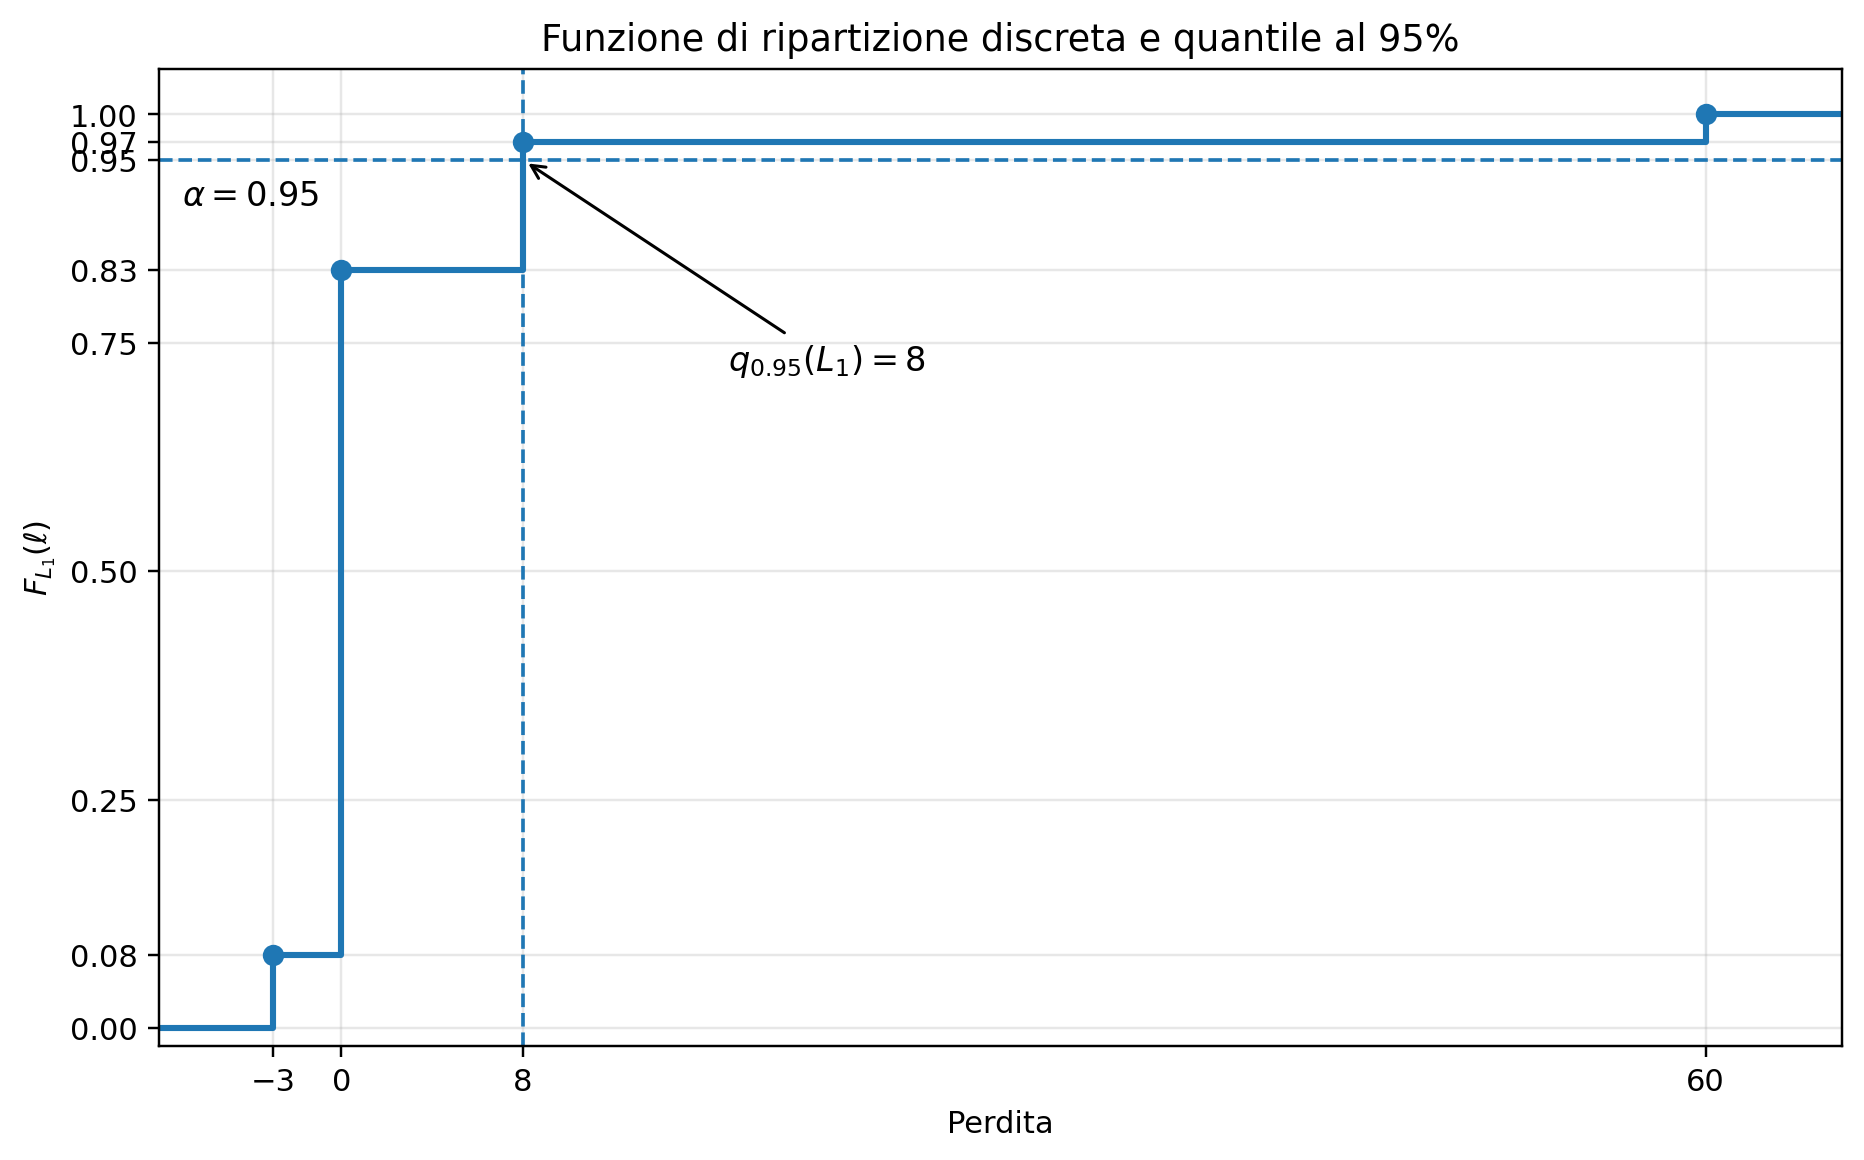
\includegraphics[width=0.82\textwidth]
{../graphics/Cap09_funzione_ripartizione_quantile.png}
\caption{Funzione di ripartizione discreta della perdita e quantile di
livello $0.95$.}
\label{fig:cap09-cdf-quantile}
\end{figure}

La discrezione della distribuzione produce anche variazioni discontinue
del quantile al variare di $\alpha$. Nell'esempio,

\[
q_{\alpha}(L_1\mid X_0=2)
=
\begin{cases}
-3,
&
0<\alpha\leq0.08,
\\[1mm]
0,
&
0.08<\alpha\leq0.83,
\\[1mm]
8,
&
0.83<\alpha\leq0.97,
\\[1mm]
60,
&
0.97<\alpha<1.
\end{cases}
\]

Il quantile \textbf{rimane costante} per interi intervalli di livelli di
probabilit\`{a} e cambia bruscamente quando $\alpha$ supera una
probabilit\`{a} cumulata.

Ad esempio,

\[
q_{0.97}(L_1\mid X_0=2)=8,
\]

mentre, per ogni valore anche di poco superiore a $0.97$,

\[
q_{\alpha}(L_1\mid X_0=2)=60.
\]

Una variazione molto piccola del livello di confidenza pu\`{o} quindi
produrre una variazione molto ampia della soglia monetaria. Questa
instabilit\`{a} non costituisce un errore di calcolo: \`{e} una
conseguenza della distribuzione discreta e della ridotta massa di
probabilit\`{a} collocata tra le perdite intermedie e il default.

\begin{remark}
Per calcolare correttamente un quantile discreto occorre:

\begin{enumerate}

\item ordinare le realizzazioni di $L_h$ in senso crescente;

\item associare a ciascuna realizzazione la relativa probabilit\`{a};

\item costruire le probabilit\`{a} cumulate nell'ordine delle perdite;

\item selezionare la prima perdita per la quale la probabilit\`{a}
cumulata raggiunge o supera $\alpha$.

\end{enumerate}
\end{remark}

L'ordinamento deve riguardare le perdite monetarie, non i codici
numerici attribuiti agli stati della catena. Inoltre, la convenzione

\[
q_{\alpha}(L)
=
\inf
\{
\ell:F_L(\ell)\geq\alpha
\}
\]

deve essere dichiarata esplicitamente. In presenza di distribuzioni
discrete, definizioni o algoritmi differenti possono trattare in modo
diverso i punti nei quali $\alpha$ coincide con una probabilit\`{a}
cumulata.

Il quantile appena definito fornisce la base matematica del Value at
Risk. Nella sezione successiva, la stessa quantit\`{a} verr\`{a}
interpretata come soglia di perdita associata a un livello di
confidenza e a un orizzonte temporale determinati.

\section{Value at Risk creditizio}

\label{sec:cap9-var-creditizio}

Il quantile introdotto nella sezione precedente pu\`{o} essere
interpretato come una soglia monetaria di rischio. Nel contesto
creditizio, tale soglia viene denominata \emph{Value at Risk} della
perdita.

\subsection{Definizione}

\label{subsec:cap9-definizione-var}

\begin{definition}
Sia $L$ una variabile casuale perdita e sia $\alpha\in(0,1)$. Il
\emph{Value at Risk} di livello $\alpha$ \`{e}

\[
\VaR_{\alpha}(L)
=
q_{\alpha}(L)
=
\inf
\left\{
\ell\in\R:
F_L(\ell)\geq\alpha
\right\}.
\]
\end{definition}

Per definizione,

\[
\Prob
\left(
L\leq\VaR_{\alpha}(L)
\right)
\geq
\alpha.
\]

In una distribuzione discreta, la probabilit\`{a} pu\`{o} essere
strettamente maggiore di $\alpha$, poich\'{e} la funzione di
ripartizione pu\`{o} superare il livello richiesto mediante un salto.

Condizionatamente allo stato iniziale $X_0=i$, indicheremo con

\[
\VaR_{\alpha,i}(h)
=
q_{\alpha}(L_h\mid X_0=i)
\]

il VaR della perdita creditizia all'orizzonte $h$.

Nell'esempio della Sezione~9.6,

\[
\VaR_{0.95,2}(1)=8,
\]

poich\'{e}

\[
\Prob(L_1\leq0\mid X_0=2)=0.83<0.95
\]

e

\[
\Prob(L_1\leq8\mid X_0=2)=0.97\geq0.95.
\]

Il risultato indica che $8$ \`{e} la pi\`{u} piccola soglia di perdita
per la quale la probabilit\`{a} cumulata raggiunge almeno il $95\%$.

\subsection{Orizzonte e livello di confidenza}

\label{subsec:cap9-orizzonte-confidenza-var}

Un valore di VaR non \`{e} interpretabile senza specificare almeno:

\begin{itemize}

\item l'orizzonte temporale $h$;

\item il livello di confidenza $\alpha$;

\item la valuta o l'unit\`{a} monetaria della perdita;

\item la distribuzione di $L_h$ e il modello utilizzato per
costruirla.

\end{itemize}

Ad esempio, l'affermazione

\begin{quote}
\emph{il VaR \`{e} pari a 8}
\end{quote}

\noindent
\`{e} incompleta. Una formulazione corretta \`{e}:

\begin{quote}
\emph{Il VaR al $95\%$ della perdita a un anno, condizionatamente al
rating iniziale $i=2$, \`{e} pari a 8 unit\`{a} monetarie nel modello
di transizione del rating considerato.}
\end{quote}

Una variazione dell'orizzonte modifica sia le probabilit\`{a} degli
stati futuri, attraverso $P^h$, sia i valori associati ai rating,
attraverso la funzione $\ell(j,h)$. Pertanto,

\[
\VaR_{\alpha,i}(h)
\]

dipende congiuntamente dal modello delle transizioni e dal modello
delle conseguenze economiche.

\subsection{Credit VaR ed economic capital}

\label{subsec:cap9-credit-var-capitale}

L'espressione \emph{Credit VaR} non viene utilizzata in modo
perfettamente uniforme. Essa pu\`{o} indicare:

\begin{itemize}

\item il quantile della distribuzione della perdita totale;

\item la perdita inattesa quantilica, ottenuta sottraendo la perdita
attesa dal quantile.

\end{itemize}

Nel presente capitolo adotteremo la seguente convenzione:

\[
\mathrm{CreditVaR}_{\alpha,i}(h)
=
\VaR_{\alpha,i}(h),
\]

ossia il Credit VaR coincide con il quantile della perdita totale.

Il capitale economico associato al livello $\alpha$ viene invece
definito come

\[
\mathrm{EC}_{\alpha,i}(h)
=
\VaR_{\alpha,i}(h)
-
\mathrm{EL}_i(h).
\]

La distinzione \`{e} quindi

\[
\begin{array}{lll}
\VaR_{\alpha,i}(h)
&
&
\text{perdita corrispondente al quantile $\alpha$,}
\\[2mm]
\mathrm{EL}_i(h)
&
&
\text{perdita media,}
\\[2mm]
\mathrm{EC}_{\alpha,i}(h)
&
&
\text{perdita quantilica eccedente la media.}
\end{array}
\]

Nell'esempio precedente,

\[
\mathrm{EL}_2(1)=2.68
\]

e

\[
\VaR_{0.95,2}(1)=8.
\]

Pertanto,

\[
\mathrm{EC}_{0.95,2}(1)
=
8-2.68
=
5.32.
\]

Il valore $5.32$ rappresenta la distanza tra la soglia di perdita al
$95\%$ e il costo medio probabilistico dell'esposizione.

\subsection{Limiti del VaR}

\label{subsec:cap9-limiti-var}

Il VaR fornisce una soglia monetaria associata a un livello di
confidenza e a un orizzonte temporale. Questa immediatezza ne facilita
l'interpretazione e la comunicazione, ma non deve nascondere alcuni
limiti importanti.

\medskip

\noindent
\textbf{Il VaR non rappresenta la massima perdita possibile.}

Poniamo

\[
v=\VaR_{\alpha}(L).
\]

Per definizione,

\[
\Prob(L\leq v)\geq\alpha.
\]

Di conseguenza,

\[
\Prob(L>v)\leq 1-\alpha.
\]

Quindi almeno una quota
$1-\alpha$ della distribuzione sar\`{a} associata a perdite superiori a
$v$ e la domanda:

\begin{quote}
\emph{Il VaR costituisce un limite superiore della perdita?}
\end{quote}

\noindent deve ricevere risposta negativa. Il VaR indica una soglia della
distribuzione, non la perdita massima realizzabile.

\medskip

\noindent
\textbf{Il VaR non descrive la severit\`{a} delle perdite oltre la
soglia.}

Una volta determinato il quantile $v$, il VaR non utilizza
l'informazione relativa all'ammontare delle perdite superiori a tale
valore. Se la parte estrema della distribuzione diventa pi\`{u} severa,
ma il quantile di livello $\alpha$ rimane invariato, anche il VaR
rimane invariato.

Due distribuzioni possono pertanto avere lo stesso VaR e presentare
perdite molto differenti negli scenari pi\`{u} sfavorevoli. Il VaR
individua il punto nel quale viene raggiunto il livello di probabilit\`{a}
$\alpha$, ma non misura la gravit\`{a} della coda successiva.

\medskip

\noindent
\textbf{Il VaR pu\`{o} non essere subadditivo.}

Una misura di rischio \`{e} subadditiva se, per due perdite $L_A$ e
$L_B$,

\[
\VaR_{\alpha}(L_A+L_B)
\leq
\VaR_{\alpha}(L_A)
+
\VaR_{\alpha}(L_B).
\]

La propriet\`{a} esprime l'idea che il rischio della posizione
aggregata non debba superare la somma dei rischi misurati separatamente.

Consideriamo ora un esempio autonomo, distinto da quelli sviluppati
nelle sezioni precedenti. Siano $L_A$ e $L_B$ le perdite relative a
due esposizioni indipendenti, entrambe caratterizzate dalla
distribuzione

\[
\begin{array}{c|cc}
\text{perdita}
&
0
&
10
\\
\hline
\text{probabilit\`{a}}
&
0.96
&
0.04
\end{array}
\]

Al livello $\alpha=0.95$,

\[
\VaR_{0.95}(L_A)
=
\VaR_{0.95}(L_B)
=
0,
\]

poich\'{e} per ciascuna esposizione

\[
\Prob(L_A\leq0)
=
\Prob(L_B\leq0)
=
0.96
\geq
0.95.
\]

La perdita aggregata $L_A+L_B$ pu\`{o} assumere i valori $0$, $10$ e
$20$. Per l'indipendenza, la sua distribuzione \`{e}

\[
\begin{array}{c|ccc}
\text{perdita aggregata}
&
0
&
10
&
20
\\
\hline
\text{probabilit\`{a}}
&
(0.96)^2
&
2(0.96)(0.04)
&
(0.04)^2
\\
\hline
&
0.9216
&
0.0768
&
0.0016
\end{array}
\]

La probabilit\`{a} cumulata in corrispondenza della perdita nulla
\`{e}

\[
\Prob(L_A+L_B\leq0)
=
0.9216
<
0.95.
\]

In corrispondenza della perdita $10$ si ha invece

\[
\begin{split}
\Prob(L_A+L_B\leq10)
&=
0.9216+0.0768
\\
&=
0.9984
\geq
0.95.
\end{split}
\]

Pertanto,

\[
\VaR_{0.95}(L_A+L_B)=10.
\]

Ne segue

\[
\VaR_{0.95}(L_A+L_B)
=
10
>
0
=
\VaR_{0.95}(L_A)
+
\VaR_{0.95}(L_B).
\]

In questo esempio il VaR viola la subadditivit\`{a}: la misura
attribuita alla posizione aggregata supera la somma delle misure
attribuite alle due esposizioni considerate separatamente.

\medskip

\noindent
\textbf{Il VaR pu\`{o} essere instabile nelle distribuzioni discrete.}

Torniamo ora alla distribuzione della perdita utilizzata nelle sezioni
precedenti. Le probabilit\`{a} cumulate associate alle perdite $8$ e
$60$ sono rispettivamente

\[
F_{L_1\mid 2}(8)=0.97
\]

e

\[
F_{L_1\mid 2}(60)=1.
\]

Di conseguenza,

\[
\VaR_{0.97,2}(1)=8,
\]

mentre, per ogni $\alpha>0.97$,

\[
\VaR_{\alpha,2}(1)=60.
\]

Un incremento anche molto piccolo del livello di confidenza pu\`{o}
quindi produrre un ampio salto della soglia monetaria. Questo
comportamento deriva dai salti della funzione di ripartizione e dalla
massa di probabilit\`{a} associata al default.

I limiti esaminati mostrano che il VaR non contiene tutta
l'informazione necessaria per valutare il rischio della coda. In
particolare, non misura l'ammontare medio delle perdite pi\`{u}
sfavorevoli. Questa informazione sar\`{a} fornita dalil CVaR, o
Expected Shortfall.

\section{CVaR ed Expected Shortfall}

\label{sec:cap9-cvar-expected-shortfall}

Il VaR individua una soglia della distribuzione, ma non descrive la
gravit\`{a} delle perdite che la superano. Per misurare anche la
severit\`{a} della coda si introduce il CVaR, normalmente denominato
anche \emph{Expected Shortfall}.

\subsection{Definizione mediante quantili}

\label{subsec:cap9-definizione-cvar}

\begin{definition}
Sia $L$ una variabile casuale perdita e sia $\alpha\in(0,1)$. Il
\emph{Conditional Value at Risk} di livello $\alpha$ \`{e}

\[
\CVaR_{\alpha}(L)
=
\frac{1}{1-\alpha}
\int_{\alpha}^{1}
q_u(L)\,du.
\]
\end{definition}

Il CVaR rappresenta la media dei quantili appartenenti alla frazione
$1-\alpha$ pi\`{u} sfavorevole della distribuzione.

Nel presente corso adotteremo la convenzione

\[
\operatorname{ES}_{\alpha}(L)
=
\CVaR_{\alpha}(L),
\]

utilizzando quindi \emph{Expected Shortfall} e CVaR come denominazioni
della stessa misura di rischio.

Per una perdita all'orizzonte $h$, condizionatamente allo stato
iniziale $X_0=i$, scriveremo

\[
\CVaR_{\alpha,i}(h)
=
\CVaR_{\alpha}(L_h\mid X_0=i).
\]

A differenza del VaR, Il CVaR dipende non soltanto dal punto in cui
inizia la coda, ma anche dall'ampiezza delle perdite che la
costituiscono.

\subsection{Rappresentazione di ottimizzazione}

\label{subsec:cap9-rappresentazione-ottimizzazione-cvar}

Il CVaR ammette la rappresentazione

\[
\boxed{
\CVaR_{\alpha}(L)
=
\min_{\eta\in\R}
\left\{
\eta
+
\frac{1}{1-\alpha}
\E\left[(L-\eta)^+\right]
\right\},
}
\]

dove

\[
(x)^+
=
\max\{x,0\}.
\]

Per un valore assegnato di $\eta$, il termine

\[
(L-\eta)^+
\]

misura soltanto l'eccesso della perdita rispetto alla soglia $\eta$.
Le realizzazioni inferiori alla soglia non producono alcun contributo.

La funzione

\[
\eta
\longmapsto
\eta
+
\frac{1}{1-\alpha}
\E\left[(L-\eta)^+\right]
\]

\`{e} convessa. Un suo minimizzatore pu\`{o} essere scelto tra i
quantili di livello $\alpha$; nelle distribuzioni discrete il
minimizzatore pu\`{o} non essere unico.

Questa rappresentazione sar\`{a} particolarmente utile quando il CVaR
verr\`{a} inserita nella funzione obiettivo o nei vincoli di un
problema di ottimizzazione.

\subsection{Distribuzioni discrete e massa nel punto di VaR}

\label{subsec:cap9-cvar-discreta}

Nelle distribuzioni continue, sotto opportune condizioni, il CVaR
pu\`{o} essere interpretata come perdita media condizionata al
superamento del VaR. Questa interpretazione non \`{e} generalmente
corretta nelle distribuzioni discrete.

Poniamo

\[
v
=
\VaR_{\alpha}(L).
\]

Se la funzione di ripartizione presenta un salto nel punto $v$, il
livello $\alpha$ pu\`{o} trovarsi all'interno della massa di
probabilit\`{a} associata a $L=v$. In tal caso,

\[
\CVaR_{\alpha}(L)
=
\frac{
v\left[F_L(v)-\alpha\right]
+
\E\left[
L\1_{\{L>v\}}
\right]
}{
1-\alpha
}.
\]

La formula comprende:

\begin{itemize}

\item tutte le perdite strettamente superiori al VaR;

\item soltanto la frazione della massa nel punto di VaR necessaria a
completare la probabilit\`{a} di coda $1-\alpha$.

\end{itemize}

Riprendiamo la distribuzione utilizzata nelle sezioni precedenti:

\[
\begin{array}{c|cccc}
L_1
&
-3
&
0
&
8
&
60
\\
\hline
\Prob(L_1=\ell\mid X_0=2)
&
0.08
&
0.75
&
0.14
&
0.03
\\
\hline
F_{L_1\mid 2}(\ell)
&
0.08
&
0.83
&
0.97
&
1.00
\end{array}
\]

Al livello $\alpha=0.95$, dalla riga della funzione di ripartizione si
osserva che

\[
F_{L_1\mid 2}(0)=0.83<0.95,
\qquad
F_{L_1\mid 2}(8)=0.97\geq0.95.
\]

Pertanto,

\[
\VaR_{0.95,2}(1)=8.
\]

Il CVaR considera la coda pi\`{u} sfavorevole della distribuzione,
avente probabilit\`{a}

\[
1-\alpha=0.05.
\]

La funzione di ripartizione raggiunge il valore $0.97$ in
corrispondenza della perdita $8$. La parte della coda compresa tra i
livelli $0.95$ e $0.97$ ha quindi probabilit\`{a}

\[
F_{L_1\mid 2}(8)-\alpha
=
0.97-0.95
=
0.02
\]

ed \`{e} associata alla perdita $8$.

La parte restante della coda, compresa tra i livelli $0.97$ e $1$, ha
probabilit\`{a}

\[
1-F_{L_1\mid 2}(8)
=
1-0.97
=
0.03
\]

ed \`{e} associata alla perdita $60$.

Normalizzando queste probabilit\`{a} rispetto alla massa complessiva
della coda, si ottengono le probabilit\`{a} condizionate

\[
\frac{0.02}{0.05}=0.40,
\qquad
\frac{0.03}{0.05}=0.60.
\]

Il CVaR \`{e} quindi il valore atteso condizionato alla coda
pi\`{u} sfavorevole di probabilit\`{a} $0.05$:

\[
\begin{split}
\CVaR_{0.95,2}(1)
&=
8\left(\frac{0.02}{0.05}\right)
+
60\left(\frac{0.03}{0.05}\right)
\\
&=
39.2.
\end{split}
\]

La probabilit\`{a} $0.02$ rappresenta la parte della massa collocata
nel punto di VaR che deve essere inclusa per completare la coda di
probabilit\`{a} $0.05$. Non viene quindi utilizzata l'intera
probabilit\`{a} $0.14$ associata alla perdita $8$.

Per questo motivo, nelle distribuzioni discrete il CVaR non coincide
in generale con

\[
\E
\left[
L_1
\mid
L_1\geq\VaR_{0.95}(L_1)
\right],
\]

poich\'{e} tale condizionamento includerebbe tutta la massa collocata
nel punto di VaR, anzich\'{e} soltanto la frazione necessaria a
costruire la coda di probabilit\`{a} $1-\alpha$.

Lo stesso risultato si ottiene dalla rappresentazione di
ottimizzazione, ponendo $\eta=8$:

\[
\begin{split}
\CVaR_{0.95,2}(1)
&=
8
+
\frac{1}{0.05}
\E\left[(L_1-8)^+\mid X_0=2\right]
\\
&=
8
+
\frac{1}{0.05}(60-8)(0.03)
\\
&=
39.2.
\end{split}
\]

Non sarebbe invece corretto calcolare semplicemente

\[
\E[L_1\mid L_1\geq8,\ X_0=2].
\]

Infatti,

\[
\begin{split}
\E[L_1\mid L_1\geq8,\ X_0=2]
&=
\frac{
(8)(0.14)+(60)(0.03)
}{
0.14+0.03
}
\\
&\approx
17.18,
\end{split}
\]

che non coincide con il CVaR. Il condizionamento $L_1\geq8$ include
l'intera massa di probabilit\`{a} associata alla perdita $8$, mentre
la coda al $5\%$ ne richiede soltanto una parte.

In generale, quindi,

\[
\boxed{
\CVaR_{\alpha}(L)
\neq
\E
\left[
L\mid L\geq\VaR_{\alpha}(L)
\right]
}
\]

quando la distribuzione presenta una massa nel punto di VaR.

\subsection{Confronto tra VaR e CVaR}

\label{subsec:cap9-confronto-var-cvar}

Consideriamo due distribuzioni di perdita:

\[
\begin{array}{c|cccc}
&
0
&
10
&
20
&
100
\\
\hline
\Prob(L_A=x)
&
0.95
&
0
&
0.05
&
0
\\
\Prob(L_B=x)
&
0.95
&
0.04
&
0
&
0.01
\end{array}
\]

Per entrambe le distribuzioni,

\[
\Prob(L_A\leq0)
=
\Prob(L_B\leq0)
=
0.95.
\]

Pertanto,

\[
\VaR_{0.95}(L_A)
=
\VaR_{0.95}(L_B)
=
0.
\]

Il VaR non distingue quindi le due esposizioni. Le rispettive code
sono per\`{o} differenti.

Per $L_A$, l'intera coda al $5\%$ \`{e} costituita dalla perdita $20$:

\[
\CVaR_{0.95}(L_A)
=
20.
\]

Per $L_B$, la coda comprende una perdita pari a $10$ con probabilit\`{a}
$0.04$ e una perdita pari a $100$ con probabilit\`{a} $0.01$:

\[
\begin{split}
\CVaR_{0.95}(L_B)
&=
\frac{
(10)(0.04)+(100)(0.01)
}{
0.05
}
\\
&=
28.
\end{split}
\]

Si ottiene quindi

\[
\VaR_{0.95}(L_A)
=
\VaR_{0.95}(L_B),
\]

ma

\[
\CVaR_{0.95}(L_A)
<
\CVaR_{0.95}(L_B).
\]

Le due distribuzioni iniziano la propria coda nello stesso punto, ma
$L_B$ presenta perdite estreme pi\`{u} severe. Il VaR individua
soltanto la soglia; il CVaR utilizza anche l'informazione contenuta
oltre tale soglia.

\section{Applicazione integrata: rischio di una singola esposizione}

\label{sec:cap9-applicazione-singola-esposizione}

Le sezioni precedenti hanno introdotto separatamente le probabilit\`{a}
di transizione, la funzione di perdita e le misure di rischio. In
questa sezione gli stessi elementi vengono riuniti in un'unica
applicazione finanziaria.

Riprendiamo la matrice di transizione annuale dei rating introdotta nel
Capitolo~8:

\[
P_R
=
\begin{pmatrix}
0.80 & 0.18 & 0.02 & 0.00\\
0.08 & 0.75 & 0.14 & 0.03\\
0.02 & 0.18 & 0.65 & 0.15\\
0.00 & 0.00 & 0.00 & 1.00
\end{pmatrix},
\]

con stati

\[
\mathcal{I}
=
\{
1=\text{alta qualit\`{a}},
\,
2=\text{qualit\`{a} intermedia},
\,
3=\text{speculative grade},
\,
D=\text{default}
\}.
\]

Lo stato $D$, equivalente allo stato $4$ del Capitolo~8, \`{e}
assorbente. Consideriamo un'obbligazione emessa da un soggetto
inizialmente appartenente alla classe di qualit\`{a} intermedia e
valutiamo il rischio a un anno.

\subsection{Probabilit\`{a} degli stati futuri}

\label{subsec:cap9-applicazione-probabilita-stati}

Lo stato iniziale \`{e}

\[
X_0=2.
\]

Poich\'{e} l'orizzonte \`{e} $h=1$, la distribuzione dei rating futuri
si legge direttamente nella seconda riga di $P_R$:

\[
\Prob(X_1=j\mid X_0=2)
=
\begin{cases}
0.08, & j=1,\\[1mm]
0.75, & j=2,\\[1mm]
0.14, & j=3,\\[1mm]
0.03, & j=D.
\end{cases}
\]

La probabilit\`{a} di default entro un anno coincide con la
probabilit\`{a} marginale di default nel primo periodo:

\[
\mathrm{PD}_{2}^{\mathrm{cum}}(1)
=
\mathrm{PD}_{2}^{\mathrm{marg}}(1)
=
(P_R)_{2D}
=
0.03.
\]

La sola probabilit\`{a} di default non descrive tuttavia l'intera
distribuzione economica dell'esposizione. Con probabilit\`{a} $0.14$
l'emittente subisce un downgrade senza entrare in default, mentre con
probabilit\`{a} $0.08$ ottiene un miglioramento del rating.

\subsection{Valori e perdite per stato}

\label{subsec:cap9-applicazione-valori-perdite}

Consideriamo un'obbligazione con

\[
N=100,
\qquad
C=4,
\qquad
T=5,
\]

dove $N$ \`{e} il valore nominale, $C$ la cedola annuale e $T$ la
scadenza. La valutazione viene effettuata alla data $h=1$,
immediatamente dopo il pagamento della prima cedola; rimangono quindi
quattro pagamenti cedolari e il rimborso finale del capitale.

Assumiamo una struttura piatta dei tassi privi di rischio con

\[
r=0.02
\]

e tassi spread creditizi dipendenti dal rating futuro:

\[
s_1=0.012,
\qquad
s_2=0.020,
\qquad
s_3=0.043.
\]

Il tasso di sconto utilizzato per valutare l'obbligazione nello stato
non-default $j$ \`{e}

\[
y_j=r+s_j.
\]

Il valore condizionato al rating futuro \`{e} quindi

\[
V_j(1)
=
\sum_{k=1}^{4}
\frac{C}{(1+y_j)^k}
+
\frac{N}{(1+y_j)^4},
\qquad
j=1,2,3.
\]

Si ottiene

\[
V_1(1)\approx102.96,
\qquad
V_2(1)=100,
\qquad
V_3(1)\approx92.08.
\]

L'aumento dello spread associato al downgrade riduce il valore
dell'obbligazione anche in assenza di default.

Per lo stato di default assumiamo un recovery rate pari al $40\%$
dell'esposizione:

\[
R=0.40,
\qquad
\mathrm{EAD}_1=100.
\]

Assumendo che il recupero sia disponibile alla data di valutazione, il
valore nello stato di default \`{e}

\[
V_D(1)
=
R \cdot \mathrm{EAD}_1
=
40.
\]

Assumiamo come valore di riferimento il valore corrispondente alla
permanenza nella classe iniziale:

\[
V^{\mathrm{ref}}(1)
=
V_2(1)
=
100.
\]

La funzione di perdita \`{e}

\[
\ell(j,1)
=
V^{\mathrm{ref}}(1)-V_j(1).
\]

I risultati sono riassunti nella tabella seguente:

\[
\begin{array}{cccccc}
\hline
\text{stato}
&
(P_R)_{2j}
&
s_j
&
y_j
&
V_j(1)
&
\ell(j,1)
\\
\hline
1
&
0.08
&
1.20\%
&
3.20\%
&
102.96
&
-2.96
\\
2
&
0.75
&
2.00\%
&
4.00\%
&
100.00
&
0.00
\\
3
&
0.14
&
4.30\%
&
6.30\%
&
92.08
&
7.92
\\
D
&
0.03
&
--
&
--
&
40.00
&
60.00
\\
\hline
\end{array}
\]

Per mantenere leggibili i calcoli e raccordare l'applicazione agli
esempi delle sezioni precedenti, utilizziamo i valori arrotondati

\[
\ell(1,1)=-3,
\qquad
\ell(2,1)=0,
\qquad
\ell(3,1)=8,
\qquad
\ell(D,1)=60.
\]

Le misure che seguono sono calcolate sui valori arrotondati. L'impiego
dei valori non arrotondati produrrebbe differenze numeriche minime,
senza modificare l'ordinamento delle perdite o la loro interpretazione
economica.

\subsection{Distribuzione completa della perdita}

\label{subsec:cap9-applicazione-distribuzione-perdita}

La perdita a un anno \`{e}

\[
L_1
=
\ell(X_1,1).
\]

Condizionatamente al rating iniziale $X_0=2$, la funzione di massa e la
funzione di ripartizione sono:

\[
\begin{array}{c|cccc}
L_1
&
-3
&
0
&
8
&
60
\\
\hline
\Prob(L_1=\ell\mid X_0=2)
&
0.08
&
0.75
&
0.14
&
0.03
\\
\hline
F_{L_1\mid 2}(\ell)
&
0.08
&
0.83
&
0.97
&
1.00
\end{array}
\]

La distribuzione contiene quattro conseguenze economiche distinte:

\[
\begin{array}{lll}
L_1=-3
&
&
\text{guadagno da miglioramento del rating,}
\\[1mm]
L_1=0
&
&
\text{assenza di variazione rispetto al riferimento,}
\\[1mm]
L_1=8
&
&
\text{perdita mark-to-market da downgrade,}
\\[1mm]
L_1=60
&
&
\text{perdita da default al netto del recupero.}
\end{array}
\]

La probabilit\`{a} cumulata raggiunge $0.83$ in corrispondenza della
perdita nulla e $0.97$ in corrispondenza della perdita $8$. Il default
occupa la parte estrema della coda, con probabilit\`{a} $0.03$.

\subsection{Misure di rischio}

\label{subsec:cap9-applicazione-misure-rischio}

La perdita attesa \`{e}

\[
\begin{split}
\mathrm{EL}_2(1)
&=
\E[L_1\mid X_0=2]
\\
&=
(-3)(0.08)
+
(0)(0.75)
+
(8)(0.14)
+
(60)(0.03)
\\
&=
2.68.
\end{split}
\]

Il secondo momento \`{e}

\[
\begin{split}
\E[L_1^2\mid X_0=2]
&=
(-3)^2(0.08)
+
8^2(0.14)
+
60^2(0.03)
\\
&=
117.68.
\end{split}
\]

Pertanto,

\[
\begin{split}
\Var(L_1\mid X_0=2)
&=
117.68-(2.68)^2
\\
&=
110.4976,
\end{split}
\]

e la deviazione standard \`{e}

\[
\sigma_{L,2}(1)
=
\sqrt{110.4976}
\approx
10.51.
\]

Consideriamo ora il livello di confidenza

\[
\alpha=0.95.
\]

Poich\'{e}

\[
F_{L_1\mid 2}(0)=0.83<0.95
\]

e

\[
F_{L_1\mid 2}(8)=0.97\geq0.95,
\]

si ottiene

\[
\VaR_{0.95,2}(1)=8.
\]

Per il calcolo del CVaR, la coda pi\`{u} sfavorevole deve avere
probabilit\`{a} $0.05$. La perdita $60$ occupa una massa pari a
$0.03$; la parte compresa tra i livelli cumulati $0.95$ e $0.97$,
pari a $0.02$, \`{e} associata alla perdita $8$. Normalizzando rispetto
alla probabilit\`{a} complessiva della coda,

\[
\begin{split}
\CVaR_{0.95,2}(1)
&=
8\left(\frac{0.02}{0.05}\right)
+
60\left(\frac{0.03}{0.05}\right)
\\
&=
39.2.
\end{split}
\]

Infine, il capitale economico quantilico \`{e}

\[
\begin{split}
\mathrm{EC}_{0.95,2}(1)
&=
\VaR_{0.95,2}(1)
-
\mathrm{EL}_2(1)
\\
&=
8-2.68
\\
&=
5.32.
\end{split}
\]

Le misure ottenute possono essere raccolte nel prospetto seguente:

\[
\begin{array}{lc}
\hline
\text{misura}
&
\text{valore}
\\
\hline
\mathrm{EL}_2(1)
&
2.68
\\
\Var(L_1\mid X_0=2)
&
110.4976
\\
\sigma_{L,2}(1)
&
10.51
\\
\VaR_{0.95,2}(1)
&
8
\\
\CVaR_{0.95,2}(1)
&
39.2
\\
\mathrm{EC}_{0.95,2}(1)
&
5.32
\\
\hline
\end{array}
\]

\subsection{Interpretazione}

\label{subsec:cap9-applicazione-interpretazione}

La perdita attesa pu\`{o} essere scomposta nei contributi associati ai
differenti stati futuri. In termini simbolici,

\[
\begin{split}
\mathrm{EL}_2(1)
&=
\sum_{j\in\mathcal{I}}
\ell(j,1)(P_R)_{2j}
\\
&=
\ell(1,1)(P_R)_{21}
+
\ell(2,1)(P_R)_{22}
\\
&\quad
+
\ell(3,1)(P_R)_{23}
+
\ell(D,1)(P_R)_{2D}.
\end{split}
\]

Sostituendo le perdite e le probabilit\`{a} di transizione,

\[
\begin{split}
\mathrm{EL}_2(1)
&=
\underbrace{(-3)(0.08)}_{\text{upgrade}}
+
\underbrace{(0)(0.75)}_{\text{permanenza}}
\\
&\quad
+
\underbrace{(8)(0.14)}_{\text{downgrade}}
+
\underbrace{(60)(0.03)}_{\text{default}} =2.68.
\end{split}
\]

I quattro contributi sono quindi

\[
-0.24,
\qquad
0,
\qquad
1.12,
\qquad
1.80.
\]

Il default fornisce il contributo positivo maggiore alla perdita
attesa, ma non \`{e} l'unica fonte di rischio. Il downgrade genera una
perdita attesa mark-to-market pari a $1.12$, mentre il miglioramento
del rating produce un guadagno atteso pari a $0.24$ e riduce la perdita
media complessiva.

Il VaR al $95\%$ \`{e} pari a $8$. Tale perdita coincide quindi con la perdita prodotta dal downgrade, non con la perdita da default.
Questo accade perch\'{e} la probabilit\`{a} cumulata raggiunge gi\`{a}
il valore $0.97$ in corrispondenza di $L_1=8$.

La perdita da default, pari a $60$, rimane interamente oltre la soglia
del VaR. Il VaR segnala dove inizia la parte pi\`{u} sfavorevole della
distribuzione, ma non riflette direttamente la distanza tra la perdita
$8$ e la perdita estrema $60$.

Il CVaR, pari a $39.2$, incorpora invece la severit\`{a} della coda. La
coda peggiore del $5\%$ comprende tutti i casi di default, che
rappresentano il $3\%$ della distribuzione, e la frazione necessaria
della massa associata al downgrade. Il valore elevato del CVaR rispetto
al VaR mostra l'importanza della perdita da default negli scenari
estremi.

Infine,

\[
\mathrm{EC}_{0.95,2}(1)=5.32
\]

misura la distanza tra la perdita corrispondente al quantile prefissato e la perdita attesa secondo
la convenzione adottata nel capitolo.

L'applicazione mette cos\`{\i} in evidenza l'intera catena logica:

\[
\boxed{
\begin{array}{c}
\text{matrice di transizione dei rating}
\\
\downarrow
\\
\text{valori condizionati agli stati}
\\
\downarrow
\\
\text{distribuzione della perdita}
\\
\downarrow
\\
\text{EL, VaR, CVaR ed economic capital}.
\end{array}
}
\]

La matrice di transizione costituisce lo scheletro probabilistico del
modello; la valutazione dell'obbligazione e il recovery rate ne
determinano le conseguenze monetarie.

\section{Misura fisica e misura risk-neutral}

\label{sec:cap9-misure-probabilita}

La matrice di transizione attribuisce probabilit\`{a} ai possibili
rating futuri. La scelta delle probabilit\`{a} dipende tuttavia dalla
domanda alla quale il modello deve rispondere.

Occorre distinguere tra:

\[
\text{misurazione del rischio}
\]

e

\[
\text{valutazione di mercato}.
\]

Le due analisi utilizzano lo stesso insieme degli stati creditizi e
possono adottare la stessa struttura markoviana, ma richiedono in
generale matrici di transizione differenti.

Supponiamo, per semplicit\`{a}, che sotto entrambe le misure il rating
segua una catena di Markov omogenea. Indicheremo con

\[
P^{\Prob}
\]

la matrice di transizione sotto la misura fisica e con

\[
P^{\Q}
\]

la matrice di transizione sotto la misura risk-neutral.

\subsection{Due domande differenti}

\label{subsec:cap9-due-domande}

La \emph{misurazione del rischio} considera le probabilit\`{a} con cui
gli stati creditizi possono effettivamente realizzarsi. La domanda
principale \`{e}:

\[
\text{quali perdite possono verificarsi e con quali probabilit\`{a}?}
\]

Questa analisi richiede probabilit\`{a} predittive, riferite
all'evoluzione reale del rating dell'emittente. Le misure di perdita
attesa, VaR e CVaR devono pertanto essere calcolate sotto la misura
fisica $\Prob$.

La \emph{valutazione di mercato} risponde invece alla domanda:

\[
\text{qual \`{e} oggi il valore di mercato dei flussi futuri?}
\]

In un modello di pricing coerente con l'assenza di arbitraggio, il
valore viene ottenuto come valore atteso, sotto la misura
risk-neutral $\Q$, dei flussi futuri opportunamente attualizzati.

La distinzione pu\`{o} essere sintetizzata come segue:

\[
\begin{array}{ccl}
\text{misurazione del rischio}
&
\longrightarrow
&
\text{probabilit\`{a} predittive sotto }\Prob,
\\[2mm]
\text{valutazione di mercato}
&
\longrightarrow
&
\text{valori attesi di flussi attualizzati sotto }\Q.
\end{array}
\]

Le probabilit\`{a} risk-neutral non rappresentano necessariamente le
frequenze con cui gli eventi creditizi si realizzeranno. Esse sono
pesi probabilistici utilizzati per riprodurre i prezzi di mercato.

\subsection{Matrice sotto la misura fisica}

\label{subsec:cap9-matrice-fisica}

Indichiamo con

\[
P^{\Prob}
=
\left(
p_{ij}^{\Prob}
\right)_{i,j\in\mathcal{I}}
\]

la matrice di transizione sotto la misura fisica, dove

\[
p_{ij}^{\Prob}
=
\Prob(X_{t+1}=j\mid X_t=i).
\]

Per una catena omogenea,

\[
\Prob(X_h=j\mid X_0=i)
=
\left[
\left(P^{\Prob}\right)^h
\right]_{ij}.
\]

La matrice $P^{\Prob}$ determina quindi la distribuzione predittiva
degli stati futuri. Data la funzione di perdita $\ell(j,h)$, si
ottiene

\[
\Prob
\left(
L_h=\ell(j,h)
\mid X_0=i
\right)
=
\left[
\left(P^{\Prob}\right)^h
\right]_{ij},
\]

quando stati differenti producono perdite differenti. Se pi\`{u}
stati producono la stessa perdita, le corrispondenti probabilit\`{a}
devono essere aggregate.

La perdita attesa sotto la misura fisica \`{e}

\[
\mathrm{EL}_{i}^{\Prob}(h)
=
\E^{\Prob}[L_h\mid X_0=i]
=
\sum_{j\in\mathcal{I}}
\ell(j,h)
\left[
\left(P^{\Prob}\right)^h
\right]_{ij}.
\]

Anche la funzione di ripartizione della perdita viene costruita
utilizzando le probabilit\`{a} fisiche:

\[
F_{L_h\mid i}^{\Prob}(\lambda)
=
\sum_{\substack{j\in\mathcal{I}:\\
\ell(j,h)\leq\lambda}}
\left[
\left(P^{\Prob}\right)^h
\right]_{ij}.
\]

Da questa distribuzione si ricavano

\[
\VaR_{\alpha,i}^{\Prob}(h)
\]

e

\[
\CVaR_{\alpha,i}^{\Prob}(h).
\]

La sequenza concettuale \`{e} dunque

\[
P^{\Prob}
\longrightarrow
\text{distribuzione predittiva dei rating}
\longrightarrow
\text{distribuzione della perdita}
\longrightarrow
\mathrm{EL}^{\Prob},
\VaR^{\Prob},
\CVaR^{\Prob}.
\]

La matrice fisica pu\`{o} essere stimata, ad esempio, mediante le
frequenze storiche delle transizioni osservate. Il suo impiego
richiede tuttavia cautela, poich\'{e} le frequenze passate possono
non rappresentare correttamente la dinamica futura in presenza di
cambiamenti macroeconomici, istituzionali o nella composizione degli
emittenti.

\subsection{Matrice sotto la misura risk-neutral}

\label{subsec:cap9-matrice-risk-neutral}

Indichiamo con

\[
P^{\Q}
=
\left(
p_{ij}^{\Q}
\right)_{i,j\in\mathcal{I}}
\]

la matrice di transizione sotto la misura risk-neutral, dove

\[
p_{ij}^{\Q}
=
\Q(X_{t+1}=j\mid X_t=i).
\]

Per una catena omogenea sotto $\Q$,

\[
\Q(X_h=j\mid X_0=i)
=
\left[
\left(P^{\Q}\right)^h
\right]_{ij}.
\]

La matrice $P^{\Q}$ non viene utilizzata per prevedere le frequenze
future dei rating. Essa fornisce i pesi probabilistici impiegati nella
valutazione di mercato dei flussi creditizi.

Sia $C_t$ il flusso aleatorio pagato alla data $t$ e sia $D(0,t)$ il
fattore di attualizzazione dalla data $t$ alla data iniziale. Il valore
di mercato al tempo zero \`{e}

\[
V_0
=
\E^{\Q}
\left[
\sum_{t=1}^{T}
D(0,t)C_t
\right].
\]

Nel caso semplificato in cui il fattore di attualizzazione sia
deterministico e il flusso alla data $t$ dipenda soltanto dallo stato
occupato, ossia

\[
C_t=c_t(X_t),
\]

si ottiene

\[
V_0
=
\sum_{t=1}^{T}
D(0,t)
\sum_{j\in\mathcal{I}}
c_t(j)
\left[
\left(P^{\Q}\right)^t
\right]_{ij}.
\]

La struttura rilevante per il pricing \`{e} quindi

\[
P^{\Q}
\longrightarrow
\text{probabilit\`{a} risk-neutral dei flussi}
\longrightarrow
\E^{\Q}
\left[
\text{flussi attualizzati}
\right]
\longrightarrow
\text{valore di mercato}.
\]

In generale,

\[
P^{\Prob}
\neq
P^{\Q}.
\]

Le probabilit\`{a} fisiche riflettono la dinamica predittiva degli
stati creditizi. Le probabilit\`{a} risk-neutral incorporano invece
anche la remunerazione richiesta dal mercato per l'esposizione al
rischio.

Di conseguenza, una matrice stimata mediante frequenze storiche non
pu\`{o} essere utilizzata automaticamente come matrice di pricing. Il
fatto che una matrice descriva adeguatamente le transizioni osservate
non implica che, utilizzata sotto $\Q$, essa riproduca i prezzi delle
obbligazioni creditizie o dei derivati di credito.

\subsection{Portata e limiti della distinzione}

\label{subsec:cap9-portata-misure}

La distinzione tra $\Prob$ e $\Q$ riguarda innanzitutto il ruolo
attribuito alle probabilit\`{a}:

\[
\begin{array}{ccl}
P^{\Prob}
&
:
&
\text{probabilit\`{a} degli scenari futuri},
\\[2mm]
P^{\Q}
&
:
&
\text{pesi probabilistici per la valutazione di mercato}.
\end{array}
\]

Questa separazione non implica tuttavia che la misurazione del rischio
e la valutazione di mercato siano sempre completamente indipendenti.

In un modello di perdita mark-to-market, le probabilit\`{a} con cui si
raggiungono i rating futuri sono generalmente determinate sotto la
misura fisica:

\[
\Prob(X_h=j\mid X_0=i)
=
\left[
\left(P^{\Prob}\right)^h
\right]_{ij}.
\]

Il valore dell'esposizione condizionato allo stato futuro $j$ pu\`{o}
invece essere un valore di mercato, ottenuto alla data $h$ mediante una
valutazione risk-neutral dei flussi successivi. In tal caso,

\[
P^{\Prob}
\longrightarrow
\text{probabilit\`{a} degli scenari},
\]

mentre

\[
P^{\Q}
\longrightarrow
V_j(h).
\]

La perdita all'orizzonte rimane

\[
L_h
=
V^{\mathrm{ref}}(h)-V_{X_h}(h),
\]

ma la sua distribuzione utilizza le probabilit\`{a} fisiche degli
stati, mentre i valori $V_j(h)$ possono incorporare una valutazione di
mercato sotto $\Q$.

Nel seguito assumeremo che la matrice $P^{\Q}$ sia assegnata. La sua
calibrazione a partire dai prezzi di obbligazioni, CDS e altri
strumenti creditizi richiede la specificazione congiunta dei tassi di
interesse, dei flussi contrattuali, del recovery rate e dei premi per
il rischio.

Tali problemi di calibrazione vengono rinviati a corsi specialistici.
Nel presente capitolo la distinzione essenziale \`{e} la seguente:

\[
\boxed{
\begin{array}{c}
P^{\Prob}
\text{ per misurare il rischio,}
\\[2mm]
P^{\Q}
\text{ per valutare i flussi di mercato.}
\end{array}
}
\]

\section{Il credit default swap}

\label{sec:cap9-cds}

La distinzione tra misura fisica e misura risk-neutral diventa
operativa nella valutazione dei derivati di credito. Consideriamo il
\emph{credit default swap}, o CDS, nella sua forma pi\`{u} semplice.

Il CDS \`{e} un contratto nel quale una parte (tipicamente il proprietario di titoli obbligazionari) acquista protezione
contro il verificarsi di un evento creditizio avverso che colpisce l'emittente dei titoli posseduti. In cambio della protezione, essa paga periodicamente un
premio alla controparte.

La valutazione del contratto viene effettuata sotto la misura
risk-neutral $\Q$. Le probabilit\`{a} di default utilizzate nel pricing
sono pertanto ricavate dalla matrice di transizione $P^{\Q}$, non dalla
matrice fisica $P^{\Prob}$.

\subsection{Struttura contrattuale}

\label{subsec:cap9-cds-struttura}

Le parti e gli elementi essenziali di un CDS sono:

\begin{itemize}

\item il \emph{protection buyer}, che acquista la protezione e paga il
premio periodico;

\item il \emph{protection seller}, che riceve i premi e si impegna a
effettuare il pagamento di protezione in caso di evento creditizio;

\item la \emph{reference entity}, ossia l'emittente al cui rischio di
credito \`{e} riferito il contratto;

\item il nozionale $N$, sul quale vengono calcolati sia i premi sia il
pagamento di protezione;

\item il premio periodico, determinato mediante uno spread contrattuale
$s$;

\item il \emph{credit event}, che nel modello semplificato coincide con
il default della reference entity;

\item il \emph{recovery rate} $R$, che determina la parte del nozionale
recuperabile dopo il default;

\item la \emph{scadenza contrattuale} $H$.

\end{itemize}

I flussi del CDS sono suddivisi in due componenti:

\[
\begin{array}{ccl}
\text{gamba dei premi}
&
:
&
\text{pagamenti effettuati dal protection buyer,}
\\[2mm]
\text{gamba di protezione}
&
:
&
\text{pagamento effettuato dal protection seller in caso di default.}
\end{array}
\]

Indichiamo con $\mathrm{PV}_{\mathrm{prot}}$ il valore attuale della
gamba di protezione e con $\mathrm{PV}_{\mathrm{prem}}(s)$ il valore
attuale della gamba dei premi, calcolata per uno spread contrattuale
$s$.

Dal punto di vista del protection buyer, il valore del CDS alla data
iniziale \`{e} quindi

\[
V_{\mathrm{CDS}}(s)
=
\mathrm{PV}_{\mathrm{prot}}
-
\mathrm{PV}_{\mathrm{prem}}(s).
\]

Per il protection seller i segni dei due flussi sono opposti.

Indichiamo con

\[
\tau_D
=
\inf\{h\geq1:X_h=D\}
\]

il tempo di primo ingresso nello stato di default e con $d_h$ il
fattore deterministico di attualizzazione dalla data $h$ alla data
iniziale.

\subsection{Gamba di protezione}

\label{subsec:cap9-cds-protezione}

Se il default si verifica alla data $h$, il protection seller paga al
protection buyer la perdita sul nozionale:

\[
N(1-R).
\]

Il valore attuale del pagamento condizionato all'evento
$\{\tau_D=h\}$ \`{e}

\[
d_hN(1-R).
\]

Poich\'{e} il pagamento viene effettuato soltanto se il primo ingresso
in default avviene alla data $h$, il valore attuale atteso della gamba
di protezione \`{e}

\[
\mathrm{PV}_{\mathrm{prot}}
=
N(1-R)
\sum_{h=1}^{H}
d_h
\Q(\tau_D=h\mid X_0=i).
\]

Le probabilit\`{a} marginali di default sono ottenute dalla matrice
risk-neutral. Poich\'{e} lo stato $D$ \`{e} assorbente,

\[
\Q(\tau_D\leq h\mid X_0=i)
=
\left[
\left(P^{\Q}\right)^h
\right]_{iD},
\]

e quindi

\[
\Q(\tau_D=h\mid X_0=i)
=
\left[
\left(P^{\Q}\right)^h
\right]_{iD}
-
\left[
\left(P^{\Q}\right)^{h-1}
\right]_{iD}.
\]

La gamba di protezione dipende dunque dalle probabilit\`{a} di primo
ingresso in default alle diverse date contrattuali, dal recovery rate
e dai fattori di attualizzazione.

\subsection{Gamba dei premi}

\label{subsec:cap9-cds-premi}

Il protection buyer paga a ogni data $h$ un premio pari a

\[
sN,
\]

purch\'{e} la reference entity sia ancora sopravvissuta oltre tale
data.

Nella convenzione temporale adottata, se il default si verifica
esattamente alla data $h$, il pagamento del premio alla stessa data
non viene effettuato. Il premio alla data $h$ viene quindi pagato
soltanto sull'evento

\[
\{\tau_D>h\}.
\]

Il valore attuale atteso della gamba dei premi \`{e}

\[
\mathrm{PV}_{\mathrm{prem}}(s)
=
sN
\sum_{h=1}^{H}
d_h
\Q(\tau_D>h\mid X_0=i).
\]

Le probabilit\`{a} di sopravvivenza sotto la misura risk-neutral sono

\[
\Q(\tau_D>h\mid X_0=i)
=
1-
\left[
\left(P^{\Q}\right)^h
\right]_{iD}.
\]

Pertanto,

\[
\mathrm{PV}_{\mathrm{prem}}(s)
=
sN
\sum_{h=1}^{H}
d_h
\left\{
1-
\left[
\left(P^{\Q}\right)^h
\right]_{iD}
\right\}.
\]

Il premio contrattuale viene moltiplicato per probabilit\`{a} di
sopravvivenza, poich\'{e} i pagamenti futuri cessano dopo il default
della reference entity.

\subsection{Premio equo del CDS}

\label{subsec:cap9-cds-premio-equilibrio}

Alla data iniziale, il premio equo $s^{*}$ rende nullo il valore del
CDS. Dal punto di vista del protection buyer, deve quindi valere

\[
V_{\mathrm{CDS}}(s^{*})=0,
\]

ossia

\[
\mathrm{PV}_{\mathrm{prem}}(s^{*})
=
\mathrm{PV}_{\mathrm{prot}}.
\]

Sostituendo le espressioni delle due gambe,

\[
s^{*}N
\sum_{h=1}^{H}
d_h
\Q(\tau_D>h\mid X_0=i)
=
N(1-R)
\sum_{h=1}^{H}
d_h
\Q(\tau_D=h\mid X_0=i).
\]

Il nozionale compare in entrambe le gambe e si semplifica. Il premio
equo \`{e} quindi

\[
s^{*}
=
(1-R)
\frac{
\displaystyle
\sum_{h=1}^{H}
d_h
\Q(\tau_D=h\mid X_0=i)
}{
\displaystyle
\sum_{h=1}^{H}
d_h
\Q(\tau_D>h\mid X_0=i)
}.
\]

Il numeratore rappresenta il valore attuale risk-neutral della perdita
unitaria attesa da default:

\[
(1-R)
\sum_{h=1}^{H}
d_h
\Q(\tau_D=h\mid X_0=i).
\]

Il denominatore rappresenta invece il valore attuale atteso di
un'unit\`{a} di premio pagata alle date nelle quali l'emittente
sopravvive:

\[
\sum_{h=1}^{H}
d_h
\Q(\tau_D>h\mid X_0=i).
\]

Il premio equo aumenta, a parit\`{a} delle altre condizioni, quando
aumentano le probabilit\`{a} risk-neutral di default o quando
diminuisce il recovery rate.

La relazione pu\`{o} essere sintetizzata come

\[
\boxed{
\text{premio equo}
=
\frac{
\text{valore attuale atteso della protezione}
}{
\text{valore attuale atteso dell'unit\`{a} di premio}
}.
}
\]

\subsection{Ipotesi semplificatrici}

\label{subsec:cap9-cds-ipotesi}

La formulazione precedente ha finalit\`{a} didattica e si basa sulle
seguenti ipotesi:

\begin{itemize}

\item le date di pagamento e di possibile default sono annuali;

\item i tassi di interesse e i fattori di attualizzazione $d_h$ sono
deterministici;

\item il recovery rate $R$ \`{e} costante;

\item il pagamento della protezione avviene alla data discreta nella
quale viene rilevato il default;

\item non viene corrisposto il premio maturato tra l'ultima data di
pagamento e la data di default;

\item se il default avviene alla data $h$, il premio previsto alla
stessa data non viene pagato;

\item il protection seller \`{e} privo di rischio di controparte;

\item non sono considerati collateral, margini, costi di transazione o
altri aggiustamenti di valutazione.

\end{itemize}

Nei contratti di mercato i premi sono normalmente pagati con frequenza
inferiore all'anno, il default pu\`{o} verificarsi tra due date di
pagamento e il premio maturato deve essere trattato esplicitamente.
Questi elementi modificano il dettaglio dei flussi, ma non la logica
fondamentale del pricing:

\[
\text{valore della gamba dei premi}
=
\text{valore della gamba di protezione}.
\]

La matrice $P^{\Q}$ collega quindi la dinamica risk-neutral dei rating
al valore del CDS:

\[
\boxed{
P^{\Q}
\longrightarrow
\begin{array}{c}
\text{probabilit\`{a} di default}
\\
\text{e di sopravvivenza}
\end{array}
\longrightarrow
\begin{array}{c}
\text{gamba di protezione}
\\
\text{e gamba dei premi}
\end{array}
\longrightarrow
s^{*}.
}
\]

\section{Copertura mediante CDS e rischio residuo}

\label{sec:cap9-copertura-cds}

Un CDS pu\`{o} essere utilizzato per ridurre le perdite associate al
default di un'esposizione creditizia. La copertura non elimina tuttavia
necessariamente tutte le componenti del rischio: il risultato dipende
dal nozionale protetto, dalla scadenza, dalla definizione contrattuale
del credit event e dalla relazione tra il valore dell'esposizione e
quello del CDS.

La distinzione tra misura fisica e misura risk-neutral rimane
essenziale. Il premio del CDS viene determinato mediante probabilit\`{a}
risk-neutral, mentre la distribuzione delle perdite della posizione
coperta deve essere valutata mediante probabilit\`{a} fisiche.

Tutte le componenti monetarie considerate nel seguito sono espresse
alla medesima data di valutazione.

\subsection{Posizione non coperta}

\label{subsec:cap9-posizione-non-coperta}

Indichiamo con $L^{\mathrm{credito}}$ la perdita dell'esposizione
creditizia in assenza di strumenti di copertura.

La perdita della posizione non coperta \`{e} quindi

\[
L^{\mathrm{unhedged}}
=
L^{\mathrm{credito}}.
\]

La sua distribuzione dipende dalle probabilit\`{a} fisiche degli stati
creditizi futuri e dalla funzione che associa a ogni stato il valore
dell'esposizione.

Nel caso dell'applicazione della Sezione~9.9,

\[
L^{\mathrm{unhedged}}
\in
\{-3,0,8,60\},
\]

con distribuzione

\[
\begin{array}{c|cccc}
L^{\mathrm{unhedged}}
&
-3
&
0
&
8
&
60
\\
\hline
\Prob
\left(
L^{\mathrm{unhedged}}=\ell
\mid X_0=2
\right)
&
0.08
&
0.75
&
0.14
&
0.03.
\end{array}
\]

La perdita da default \`{e} pari a $60$, mentre la perdita da downgrade
\`{e} pari a $8$.

\subsection{Posizione coperta}

\label{subsec:cap9-posizione-coperta}

Indichiamo con $\Pi^{\mathrm{CDS}}$ il pagamento ricevuto dal CDS e con
$C^{\mathrm{premi}}$ il costo complessivo dei premi. Dal punto di vista
del protection buyer, la perdita della posizione coperta \`{e}

\[
L^{\mathrm{hedged}}
=
L^{\mathrm{credito}}
-
\Pi^{\mathrm{CDS}}
+
C^{\mathrm{premi}}.
\]

Il pagamento del CDS riduce la perdita, mentre il costo dei premi la
aumenta.

Nella rappresentazione semplificata con copertura del solo default,

\[
\Pi^{\mathrm{CDS}}
=
N_{\mathrm{CDS}}
\left(
1-R_{\mathrm{CDS}}
\right)
\1_{\{\tau_D\leq H\}},
\]

dove $N_{\mathrm{CDS}}$ \`{e} il nozionale del contratto e
$R_{\mathrm{CDS}}$ il recovery rate previsto ai fini del regolamento
della protezione.

La copertura \`{e} completa rispetto alla perdita da default soltanto
se

\[
N_{\mathrm{CDS}}
\left(
1-R_{\mathrm{CDS}}
\right)
\]

coincide con la perdita effettivamente subita sull'esposizione in caso
di default. Anche in questo caso rimangono il costo dei premi e le
eventuali perdite prodotte dalle variazioni del merito creditizio che
non determinano un credit event.

Prendendo il valore atteso sotto la misura fisica, si ottiene

\[
\begin{split}
\E^{\Prob}
\left[
L^{\mathrm{hedged}}
\right]
&=
\E^{\Prob}
\left[
L^{\mathrm{unhedged}}
\right]
-
\E^{\Prob}
\left[
\Pi^{\mathrm{CDS}}
\right]
\\
&\quad
+
\E^{\Prob}
\left[
C^{\mathrm{premi}}
\right].
\end{split}
\]

Pertanto, la variazione della perdita attesa \`{e}

\[
\E^{\Prob}
\left[
L^{\mathrm{hedged}}
\right]
-
\E^{\Prob}
\left[
L^{\mathrm{unhedged}}
\right]
=
\E^{\Prob}
\left[
C^{\mathrm{premi}}
\right]
-
\E^{\Prob}
\left[
\Pi^{\mathrm{CDS}}
\right].
\]

La copertura riduce la perdita attesa soltanto quando il valore atteso
fisico della protezione supera il costo atteso dei premi. Questa
condizione non \`{e} garantita dal fatto che il CDS sia stato stipulato
a un premio equo sotto la misura risk-neutral.

\subsection{Confronto delle distribuzioni}

\label{subsec:cap9-confronto-distribuzioni-copertura}

Il confronto tra posizione coperta e non coperta non pu\`{o} limitarsi
alla perdita attesa. Occorre ricostruire l'intera distribuzione di

\[
L^{\mathrm{hedged}}
=
L^{\mathrm{credito}}
-
\Pi^{\mathrm{CDS}}
+
C^{\mathrm{premi}}
\]

e calcolare separatamente

\[
\E^{\Prob}
\left[
L^{\mathrm{hedged}}
\right],
\qquad
\VaR_{\alpha}^{\Prob}
\left(
L^{\mathrm{hedged}}
\right),
\qquad
\CVaR_{\alpha}^{\Prob}
\left(
L^{\mathrm{hedged}}
\right).
\]

In generale, non valgono relazioni additive semplici per il VaR e il
CVaR. Il pagamento del CDS, la perdita creditizia e il costo dei premi
dipendono infatti dagli stessi eventi creditizi.

Consideriamo un esempio costruito sulla distribuzione della
Sezione~9.9. Supponiamo che il CDS:

\begin{itemize}

\item paghi $60$ in caso di default;

\item non effettui alcun pagamento negli altri stati;

\item richieda un premio unico anticipato, espresso in valore
equivalente alla data di analisi, pari a $2$.

\end{itemize}

Si ha quindi

\[
\Pi^{\mathrm{CDS}}
=
60\1_{\{X_1=D\}},
\qquad
C^{\mathrm{premi}}=2.
\]

La perdita della posizione coperta nei differenti stati \`{e}

\[
\begin{array}{c|ccccc}
\text{stato}
&
\Prob(X_1=j\mid X_0=2)
&
L^{\mathrm{credito}}
&
\Pi^{\mathrm{CDS}}
&
C^{\mathrm{premi}}
&
L^{\mathrm{hedged}}
\\
\hline
1
&
0.08
&
-3
&
0
&
2
&
-1
\\
2
&
0.75
&
0
&
0
&
2
&
2
\\
3
&
0.14
&
8
&
0
&
2
&
10
\\
D
&
0.03
&
60
&
60
&
2
&
2
\end{array}
\]

La protezione elimina la perdita lorda da default, ma il costo del
premio rimane anche nello stato di default. Inoltre, negli stati
non-default, il premio si aggiunge alla perdita o riduce il guadagno
della posizione creditizia.

Poich\'{e} gli stati $2$ e $D$ producono entrambi una perdita coperta
pari a $2$, le loro probabilit\`{a} devono essere aggregate. La
distribuzione della posizione coperta \`{e}

\[
\begin{array}{c|ccc}
L^{\mathrm{hedged}}
&
-1
&
2
&
10
\\
\hline
\Prob
\left(
L^{\mathrm{hedged}}=\ell
\mid X_0=2
\right)
&
0.08
&
0.78
&
0.14
\\
\hline
F_{L^{\mathrm{hedged}}\mid 2}(\ell)
&
0.08
&
0.86
&
1.00.
\end{array}
\]

La perdita attesa della posizione coperta si ottiene sommando ciascun
possibile valore della perdita, ponderato per la corrispondente
probabilit\`{a}. In termini simbolici,

\[
\E^{\Prob}
\left[
L^{\mathrm{hedged}}
\mid X_0=2
\right]
=
\sum_{\lambda\in\mathcal{L}^{\mathrm{hedged}}}
\lambda
\Prob
\left(
L^{\mathrm{hedged}}=\lambda
\mid X_0=2
\right),
\]

dove

\[
\mathcal{L}^{\mathrm{hedged}}
=
\{-1,2,10\}.
\]

Sostituendo i valori della distribuzione,

\[
\begin{split}
\E^{\Prob}
\left[
L^{\mathrm{hedged}}
\mid X_0=2
\right]
&=
(-1)(0.08)
+
(2)(0.78)
+
(10)(0.14)
\\
&=
2.88.
\end{split}
\]

Il medesimo risultato pu\`{o} essere ottenuto osservando che

\[
\E^{\Prob}
\left[
\Pi^{\mathrm{CDS}}
\mid X_0=2
\right]
=
(60)(0.03)
=
1.80.
\]

Pertanto,

\[
\begin{split}
\E^{\Prob}
\left[
L^{\mathrm{hedged}}
\mid X_0=2
\right]
&=
2.68-1.80+2
\\
&=
2.88.
\end{split}
\]

Al livello $\alpha=0.95$,

\[
F_{L^{\mathrm{hedged}}\mid 2}(2)
=
0.86
<
0.95,
\]

mentre

\[
F_{L^{\mathrm{hedged}}\mid 2}(10)
=
1
\geq
0.95.
\]

Di conseguenza,

\[
\VaR_{0.95}^{\Prob}
\left(
L^{\mathrm{hedged}}
\right)
=
10.
\]

La coda peggiore di probabilit\`{a} $0.05$ \`{e} interamente
contenuta nella massa associata alla perdita $10$. Pertanto,

\[
\CVaR_{0.95}^{\Prob}
\left(
L^{\mathrm{hedged}}
\right)
=
10.
\]
come evidenziato nella figura \ref{fig:cap09-cdf-hedged-var-cvar}

\begin{figure}[htbp]
\centering
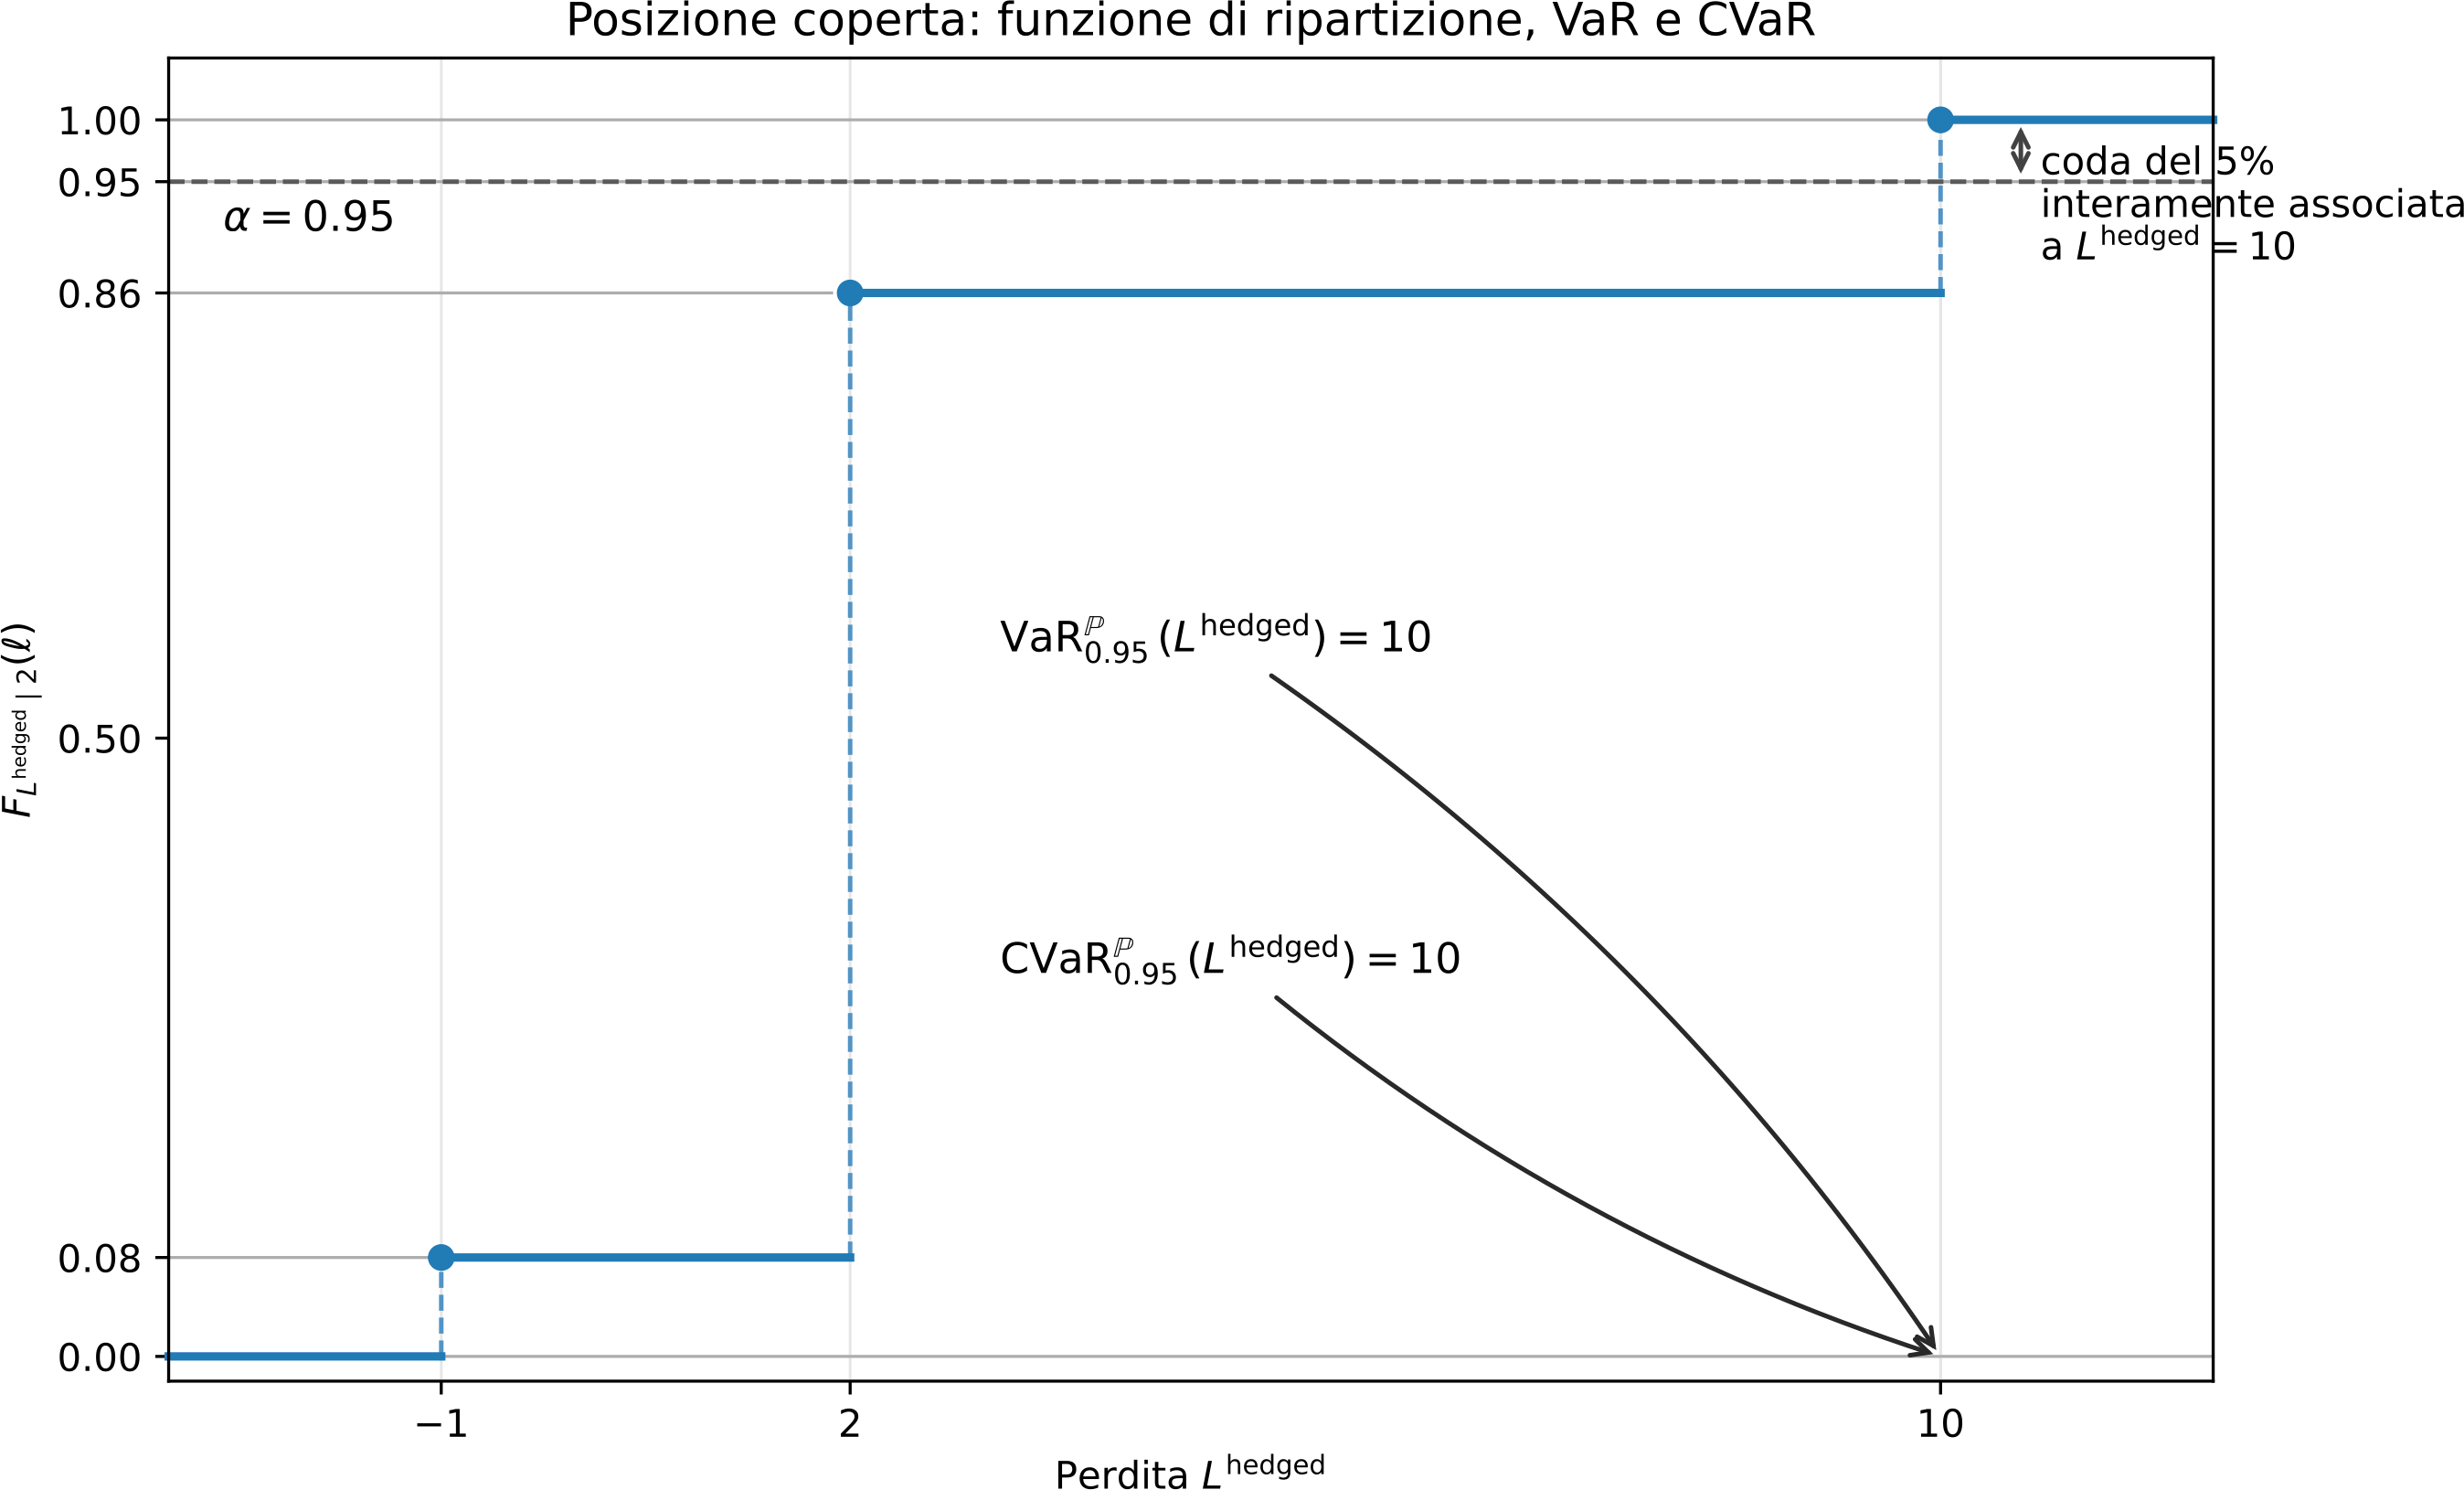
\includegraphics[width=0.82\textwidth]
{../graphics/Cap09_cdf_hedged_var_cvar.png}
\caption{Funzione di ripartizione della perdita della posizione coperta.
Al livello $\alpha=0.95$, si ha $\VaR_{0.95}^{\Prob}(L^{\mathrm{hedged}})=10$.
La coda peggiore di probabilit\`{a} $0.05$ \`{e} interamente contenuta
nell'atomo in corrispondenza della perdita $10$, e quindi
$\CVaR_{0.95}^{\Prob}(L^{\mathrm{hedged}})=10$.}
\label{fig:cap09-cdf-hedged-var-cvar}
\end{figure}


Il confronto complessivo \`{e}

\[
\begin{array}{lcc}
\hline
\text{misura}
&
\text{posizione non coperta}
&
\text{posizione coperta}
\\
\hline
\E^{\Prob}[L]
&
2.68
&
2.88
\\
\VaR_{0.95}^{\Prob}(L)
&
8
&
10
\\
\CVaR_{0.95}^{\Prob}(L)
&
39.2
&
10
\\
\hline
\end{array}
\]

La copertura riduce fortemente il CVaR, poich\'{e} elimina la perdita
estrema da default. Nello stesso esempio, tuttavia, la perdita attesa
aumenta da $2.68$ a $2.88$, poich\'{e}

\[
C^{\mathrm{premi}}
=
2
>
1.80
=
\E^{\Prob}
\left[
\Pi^{\mathrm{CDS}}
\right].
\]

Anche il VaR aumenta, passando da $8$ a $10$. Il premio certo sposta
infatti verso destra le perdite negli stati non-default e porta la
perdita da downgrade da $8$ a $10$.

Non vi \`{e} contraddizione tra questi risultati. Il CDS modifica la
forma dell'intera distribuzione: pu\`{o} ridurre la severit\`{a} della
coda estrema e, contemporaneamente, aumentare la perdita media o un
determinato quantile.

Il costo $2$ non deve essere interpretato come valore atteso fisico
della protezione. Il premio contrattuale viene determinato sotto la
misura risk-neutral, mentre le misure di rischio della posizione
coperta sono calcolate sotto la misura fisica.

\subsection{Limiti della copertura}

\label{subsec:cap9-limiti-copertura-cds}

La riduzione del rischio ottenuta mediante un CDS dipende dalla
corrispondenza tra il contratto di protezione e l'esposizione
sottostante.

\paragraph{Basis risk.}

Il valore dell'esposizione e quello del CDS possono reagire in modo
differente alle variazioni del merito creditizio, della liquidit\`{a}
e delle condizioni di mercato. Il differenziale tra lo spread
dell'obbligazione e lo spread del CDS pu\`{o} quindi variare nel tempo.
La copertura basata sul CDS non replica necessariamente in modo esatto
le variazioni di valore dell'esposizione.

\paragraph{Mismatch di nozionale.}

Se il nozionale del CDS differisce dall'esposizione effettiva, il
pagamento di protezione pu\`{o} essere insufficiente oppure eccedere la
perdita creditizia. Nel primo caso rimane una quota di rischio non
coperta; nel secondo si determina una posizione sovracoperta.

\paragraph{Mismatch di scadenza.}

La scadenza del CDS pu\`{o} essere anteriore o posteriore rispetto a
quella dell'esposizione. Se la protezione termina prima
dell'esposizione, il rischio di default riemerge dopo la scadenza del
CDS. Se la protezione ha durata superiore, possono essere sostenuti
premi relativi a un periodo nel quale l'esposizione non \`{e} pi\`{u}
presente.

\paragraph{Perdite da migrazione.}

Nella formulazione basata sul solo pagamento al credit event, il CDS
non effettua alcun pagamento in seguito a un semplice downgrade. La
perdita mark-to-market dell'obbligazione pu\`{o} quindi rimanere
scoperta.

In una valutazione mark-to-market, il valore del CDS tende a crescere
quando peggiora la qualit\`{a} creditizia della reference entity e
pu\`{o} compensare parzialmente la perdita dell'obbligazione. La
compensazione non \`{e} tuttavia necessariamente completa, a causa del
basis risk, della diversa scadenza e della diversa sensibilit\`{a}
degli strumenti agli spread.

\paragraph{Rischio di controparte.}

La protezione \`{e} efficace soltanto se il protection seller \`{e} in
grado di effettuare il pagamento previsto dal contratto. Il default o
il deterioramento della controparte pu\`{o} ridurre il valore della
copertura proprio negli scenari nei quali la protezione risulta
necessaria.

\paragraph{Evento economico ed evento contrattuale.}

Un grave deterioramento economico dell'emittente non coincide
necessariamente con un credit event riconosciuto dal contratto. Il
pagamento del CDS dipende dalla definizione giuridica e contrattuale
dell'evento creditizio, non dalla sola presenza di una perdita
economica sull'esposizione.

La qualit\`{a} della copertura deve quindi essere valutata confrontando
le distribuzioni complete delle due posizioni:

\[
L^{\mathrm{unhedged}}
\qquad
\text{e}
\qquad
L^{\mathrm{hedged}}.
\]

Una riduzione del CVaR non implica necessariamente una riduzione della
perdita attesa o del VaR. Le differenti misure descrivono aspetti
diversi della distribuzione e possono muoversi in direzioni opposte
quando il pagamento di protezione elimina gli eventi estremi, mentre
il costo dei premi incide su tutti o su molti degli altri stati.

\section{Dal singolo emittente al portafoglio}

\label{sec:cap9-portafoglio}

Le sezioni precedenti hanno considerato il rischio di una singola
esposizione. Un portafoglio creditizio contiene invece numerosi
emittenti, eventualmente caratterizzati da rating iniziali,
esposizioni, recovery rate e matrici di transizione differenti.

Il passaggio dal singolo emittente al portafoglio non consiste nella
sola somma delle probabilit\`{a} marginali. Occorre specificare anche
come le migrazioni dei rating e i default dei differenti emittenti
dipendano tra loro.

Salvo diversa indicazione, in questa sezione le probabilit\`{a} e le
misure di rischio sono considerate sotto la misura fisica $\Prob$.

\subsection{Perdita aggregata}

\label{subsec:cap9-perdita-portafoglio}

Consideriamo un portafoglio formato da $N$ esposizioni. Per
l'esposizione $n$, indichiamo con $X_{n,h}$ il rating alla data $h$ e
con

\[
L_{n,h}
=
\ell_n(X_{n,h},h)
\]

la corrispondente perdita.

La funzione $\ell_n$ pu\`{o} dipendere dalle caratteristiche
specifiche dell'esposizione, tra le quali:

\[
\mathrm{EAD}_{n,h},
\qquad
\mathrm{LGD}_{n,h},
\qquad
\text{scadenza},
\qquad
\text{struttura dei flussi}.
\]

Nel modello default-only, ad esempio,

\[
L_{n,h}
=
\mathrm{EAD}_{n,h}
\mathrm{LGD}_{n,h}
\1_{\{\tau_{D,n}\leq h\}},
\]

dove $\tau_{D,n}$ indica il tempo di default dell'emittente $n$.

Nel modello basato sulle migrazioni del rating, invece,

\[
L_{n,h}
=
V_n^{\mathrm{ref}}(h)
-
V_{n,X_{n,h}}(h),
\]

cosicch\'{e} la perdita pu\`{o} essere generata anche da un downgrade
che non determina il default.

La perdita aggregata del portafoglio all'orizzonte $h$ \`{e}

\[
L_h^{\mathrm{port}}
=
\sum_{n=1}^{N}
L_{n,h}.
\]

Per linearit\`{a} del valore atteso,

\[
\E^{\Prob}
\left[
L_h^{\mathrm{port}}
\right]
=
\sum_{n=1}^{N}
\E^{\Prob}
\left[
L_{n,h}
\right].
\]

Questa relazione vale indipendentemente dalla struttura di dipendenza
tra le esposizioni. Per calcolare la perdita attesa del portafoglio
sono quindi sufficienti le distribuzioni marginali delle singole
perdite.

La varianza della perdita aggregata \`{e} invece

\[
\begin{split}
\Var^{\Prob}
\left(
L_h^{\mathrm{port}}
\right)
&=
\sum_{n=1}^{N}
\Var^{\Prob}(L_{n,h})
\\
&\quad
+
2
\sum_{n=1}^{N-1}
\sum_{m=n+1}^{N}
\Cov^{\Prob}(L_{n,h},L_{m,h}).
\end{split}
\]

Le covarianze mostrano che la dispersione della perdita di portafoglio
dipende dal modo in cui le perdite individuali tendono a verificarsi
congiuntamente.

La dipendenza diventa ancora pi\`{u} importante per il VaR e il CVaR,
che dipendono dalla forma complessiva della distribuzione aggregata e
non possono essere ricavati sommando le corrispondenti misure
marginali.

In generale,

\[
\VaR_{\alpha}^{\Prob}
\left(
\sum_{n=1}^{N}L_{n,h}
\right)
\neq
\sum_{n=1}^{N}
\VaR_{\alpha}^{\Prob}(L_{n,h}),
\]

e analogamente il CVaR del portafoglio deve essere calcolato sulla
distribuzione di $L_h^{\mathrm{port}}$.

\subsection{Distribuzioni marginali e distribuzione congiunta}

\label{subsec:cap9-marginali-congiunta}

Per ciascun emittente $n=1,...,N$, la matrice di transizione
$P_n^{\Prob}$ determina la distribuzione del suo rating futuro. Se
l'emittente parte dal rating $i_n$, si ha

\[
\Prob
\left(
X_{n,h}=j
\mid
X_{n,0}=i_n
\right)
=
\left[
\left(P_n^{\Prob}\right)^h
\right]_{i_nj}.
\]

Queste probabilit\`{a} descrivono il comportamento del singolo
emittente considerato separatamente dagli altri. Esse costituiscono la
distribuzione marginale del rating $X_{n,h}$.

Attraverso la funzione di perdita $\ell_n$, dalla distribuzione del
rating si ricava la distribuzione marginale della perdita individuale

\[
L_{n,h}
=
\ell_n(X_{n,h},h).
\]

Per ciascun emittente $n$, la matrice di transizione
$P_n^{\Prob}$ determina la distribuzione del rating futuro,
condizionatamente al rating iniziale dell'emittente stesso:

\[
\Prob
\left(
X_{n,h}=j
\mid
X_{n,0}=i_n
\right)
=
\left[
\left(P_n^{\Prob}\right)^h
\right]_{i_nj}.
\]

Queste probabilit\`{a} descrivono separatamente i possibili rating
futuri di ciascun emittente. Esse determinano quindi le distribuzioni
individuali delle variabili

\[
X_{1,h},
X_{2,h},
\ldots,
X_{N,h}.
\]

Per rappresentare congiuntamente i rating futuri dell'intero
portafoglio introduciamo il vettore

\[
\mathbf{X}_h
=
\left(
X_{1,h},
X_{2,h},
\ldots,
X_{N,h}
\right),
\]

e il corrispondente vettore dei rating iniziali

\[
\mathbf{X}_0
=
\left(
X_{1,0},
X_{2,0},
\ldots,
X_{N,0}
\right).
\]

Rispetto al vettore $\mathbf{X}_h$, le distribuzioni individuali dei
singoli rating sono dette \emph{distribuzioni marginali}. Esse
indicano le probabilit\`{a} dei possibili rating futuri di ciascun
emittente considerato separatamente, ma non specificano con quali
probabilit\`{a} tali rating si realizzino simultaneamente.

Per descrivere le realizzazioni simultanee occorre invece conoscere la
distribuzione congiunta del vettore $\mathbf{X}_h$. Essa assegna una
probabilit\`{a} a ogni possibile configurazione dei rating futuri:

\[
\begin{split}
&
\Prob
\left(
\mathbf{X}_h=(j_1,\ldots,j_N)
\mid
\mathbf{X}_0=(i_1,\ldots,i_N)
\right)
\\
&=
\Prob
\left(
X_{1,h}=j_1,
\ldots,
X_{N,h}=j_N
\mid
X_{1,0}=i_1,
\ldots,
X_{N,0}=i_N
\right).
\end{split}
\]

La distribuzione congiunta \`{e} necessaria per determinare la
distribuzione della perdita aggregata

\[
L_h^{\mathrm{port}}
=
\sum_{n=1}^{N}
\ell_n(X_{n,h},h).
\]

Le matrici di transizione dei singoli emittenti determinano dunque le
distribuzioni marginali dei rating e delle corrispondenti perdite, ma
non determinano la distribuzione congiunta delle loro realizzazioni e,
di conseguenza, non sono sufficienti per ricavare la distribuzione
della perdita di portafoglio.

La relazione fondamentale \`{e}

\[
\boxed{
\begin{array}{c}
\text{matrici di transizione dei singoli emittenti}
\\[1mm]
\downarrow
\\[1mm]
\text{distribuzioni individuali dei rating}
\\
\text{e delle corrispondenti perdite}
\\[3mm]
\not\Longrightarrow
\\[3mm]
\text{distribuzione della perdita aggregata}
\end{array}
}
\]


Soltanto assumendo indipendenza tra le migrazioni si potrebbe scrivere

\[
\begin{split}
&
\Prob
\left(
X_{1,h}=j_1,\ldots,X_{N,h}=j_N
\mid
\mathbf{X}_0=\mathbf{i}
\right)
\\
&=
\prod_{n=1}^{N}
\Prob
\left(
X_{n,h}=j_n
\mid
X_{n,0}=i_n
\right).
\end{split}
\]

L'indipendenza costituisce tuttavia un'ipotesi particolarmente forte, e nella pratica poco realistica.
Durante una recessione, una crisi settoriale o uno shock finanziario,
pi\`{u} emittenti possono subire simultaneamente downgrade o default.

\begin{example}

Consideriamo un portafoglio formato da due emittenti. Il vettore dei
rating iniziali \`{e}

\[
\mathbf{X}_0
=
\left(
X_{1,0},
X_{2,0}
\right).
\]

Supponiamo che entrambi gli emittenti appartengano inizialmente alla
classe di rating $2$:

\[
\mathbf{X}_0
=
\mathbf{i}
=
(2,2).
\]

All'orizzonte $h$, ciascun emittente pu\`{o} soltanto permanere nello
stato $2$ oppure entrare nello stato di default $D$:

\[
X_{1,h},X_{2,h}
\in
\{2,D\}.
\]

Il vettore dei rating futuri \`{e}

\[
\mathbf{X}_h
=
\left(
X_{1,h},
X_{2,h}
\right).
\]

Le sue possibili realizzazioni sono

\[
\mathbf{j}
\in
\{
(2,2),
(D,2),
(2,D),
(D,D)
\}.
\]

Per la configurazione iniziale fissata $\mathbf{i}=(2,2)$, indichiamo
con

\[
p_h(\mathbf{i},\mathbf{j})
=
\Prob
\left(
\mathbf{X}_h=\mathbf{j}
\mid
\mathbf{X}_0=\mathbf{i}
\right)
\]

la probabilit\`{a} della configurazione futura $\mathbf{j}$.

Al variare di $\mathbf{j}$, le quantit\`{a}
$p_h(\mathbf{i},\mathbf{j})$ costituiscono la distribuzione congiunta
dei rating futuri, condizionata alla configurazione iniziale
$\mathbf{i}$.

Supponiamo che entrambi gli emittenti abbiano probabilit\`{a}
individuale di default pari a $0.05$:

\[
\Prob
\left(
X_{1,h}=D
\mid
\mathbf{X}_0=\mathbf{i}
\right)
=
\Prob
\left(
X_{2,h}=D
\mid
\mathbf{X}_0=\mathbf{i}
\right)
=
0.05.
\]

Le corrispondenti probabilit\`{a} di permanenza nello stato $2$ sono
pari a $0.95$. Confronteremo due diverse distribuzioni congiunte,
entrambe compatibili con queste stesse distribuzioni marginali.

\paragraph{Primo modello: default indipendenti.}

Se i rating futuri dei due emittenti sono indipendenti,
condizionatamente alla configurazione iniziale, la distribuzione
congiunta \`{e}

\[
\begin{array}{c|cc|c}
&
X_{2,h}=2
&
X_{2,h}=D
&
\text{totale}
\\
\hline
X_{1,h}=2
&
0.9025
&
0.0475
&
0.95
\\
X_{1,h}=D
&
0.0475
&
0.0025
&
0.05
\\
\hline
\text{totale}
&
0.95
&
0.05
&
1
\end{array}
\]

Le somme di riga forniscono la distribuzione marginale di $X_{1,h}$,
mentre le somme di colonna forniscono la distribuzione marginale di
$X_{2,h}$.

In particolare,

\[
\Prob
\left(
X_{1,h}=D
\mid
\mathbf{X}_0=\mathbf{i}
\right)
=
0.0475+0.0025
=
0.05,
\]

e

\[
\Prob
\left(
X_{2,h}=D
\mid
\mathbf{X}_0=\mathbf{i}
\right)
=
0.0475+0.0025
=
0.05.
\]

La probabilit\`{a} congiunta del doppio default \`{e}

\[
\Prob
\left(
X_{1,h}=D,
X_{2,h}=D
\mid
\mathbf{X}_0=\mathbf{i}
\right)
=
0.0025.
\]

\paragraph{Secondo modello: default perfettamente dipendenti.}

Supponiamo ora che i due emittenti subiscano sempre il default
congiuntamente. La distribuzione congiunta diventa

\[
\begin{array}{c|cc|c}
&
X_{2,h}=2
&
X_{2,h}=D
&
\text{totale}
\\
\hline
X_{1,h}=2
&
0.95
&
0
&
0.95
\\
X_{1,h}=D
&
0
&
0.05
&
0.05
\\
\hline
\text{totale}
&
0.95
&
0.05
&
1
\end{array}
\]

Le probabilit\`{a} marginali sono rimaste invariate:

\[
\Prob
\left(
X_{1,h}=D
\mid
\mathbf{X}_0=\mathbf{i}
\right)
=
0.05,
\]

e

\[
\Prob
\left(
X_{2,h}=D
\mid
\mathbf{X}_0=\mathbf{i}
\right)
=
0.05.
\]

La probabilit\`{a} congiunta del doppio default \`{e} invece

\[
\Prob
\left(
X_{1,h}=D,
X_{2,h}=D
\mid
\mathbf{X}_0=\mathbf{i}
\right)
=
0.05.
\]

Le due distribuzioni congiunte hanno pertanto gli stessi margini, ma
attribuiscono probabilit\`{a} differenti alle realizzazioni
simultanee:

\[
\begin{array}{c|cc}
&
\text{indipendenza}
&
\text{dipendenza perfetta}
\\
\hline
\Prob
\left(
X_{1,h}=D,
X_{2,h}=D
\mid
\mathbf{X}_0=\mathbf{i}
\right)
&
0.0025
&
0.05
\end{array}
\]

Supponiamo infine che ciascuna esposizione produca una perdita unitaria
in caso di default:

\[
L_{1,h}
=
\1_{\{X_{1,h}=D\}},
\qquad
L_{2,h}
=
\1_{\{X_{2,h}=D\}}.
\]

La perdita aggregata \`{e}

\[
L_h^{\mathrm{port}}
=
L_{1,h}+L_{2,h}.
\]

La corrispondenza tra configurazioni dei rating e perdita aggregata
\`{e}

\[
\begin{array}{c|cccc}
\mathbf{X}_h
&
(2,2)
&
(D,2)
&
(2,D)
&
(D,D)
\\
\hline
L_h^{\mathrm{port}}
&
0
&
1
&
1
&
2
\end{array}
\]

Nel modello con default indipendenti si ottiene

\[
\begin{array}{c|ccc}
L_h^{\mathrm{port}}
&
0
&
1
&
2
\\
\hline
\Prob
\left(
L_h^{\mathrm{port}}=\ell
\mid
\mathbf{X}_0=\mathbf{i}
\right)
&
0.9025
&
0.0950
&
0.0025
\end{array}
\]

Nel modello con default perfettamente dipendenti si ottiene invece

\[
\begin{array}{c|ccc}
L_h^{\mathrm{port}}
&
0
&
1
&
2
\\
\hline
\Prob
\left(
L_h^{\mathrm{port}}=\ell
\mid
\mathbf{X}_0=\mathbf{i}
\right)
&
0.95
&
0
&
0.05
\end{array}
\]

Le distribuzioni marginali dei rating individuali sono identiche nei
due modelli. La diversa struttura di dipendenza modifica tuttavia la
distribuzione congiunta dei rating e, di conseguenza, la distribuzione
della perdita aggregata.

\end{example}

\subsection{Concentrazione e fattori comuni}

\label{subsec:cap9-concentrazione-fattori}

La dipendenza tra le perdite pu\`{o} derivare da fattori economici
comuni e dalla composizione del portafoglio.

\paragraph{Concentrazione per debitore.}

Un portafoglio \`{e} concentrato per debitore quando una parte
rilevante dell'esposizione complessiva dipende da pochi emittenti. Se

\[
w_n
=
\frac{
\mathrm{EAD}_{n,h}
}{
\displaystyle
\sum_{m=1}^{N}
\mathrm{EAD}_{m,h}
},
\]

un valore elevato di $w_n$ indica che il deterioramento del debitore
$n$ pu\`{o} produrre una quota rilevante della perdita totale.

La presenza di molti emittenti non garantisce quindi
automaticamente una diversificazione effettiva, se il portafoglio
rimane dominato da poche esposizioni di grandi dimensioni.

\paragraph{Concentrazione settoriale.}

Emittenti appartenenti allo stesso settore possono reagire in modo
simile a variazioni dei prezzi delle materie prime, dei tassi di
interesse, della domanda o della regolamentazione.

Un portafoglio composto da numerosi debitori dello stesso settore pu\`{o}
essere poco diversificato, anche quando nessuna singola esposizione
risulta dominante.

\paragraph{Concentrazione geografica.}

La localizzazione degli emittenti in una stessa area economica espone
il portafoglio a shock comuni relativi alla crescita, alla politica
fiscale, al sistema bancario, al rischio sovrano o al quadro
istituzionale.

La diversificazione per numero di debitori pu\`{o} quindi essere
inefficace se le esposizioni rimangono concentrate nella stessa
economia.

\paragraph{Dipendenza macroeconomica.}

Le probabilit\`{a} di transizione possono dipendere da un fattore
macroeconomico comune $Z_h$, ad esempio uno stato di espansione,
rallentamento o recessione.

Condizionatamente a $Z_h$, le transizioni individuali possono essere
modellate come indipendenti:

\[
\begin{split}
&
\Prob
\left(
X_{1,h}=j_1,\ldots,X_{N,h}=j_N
\mid
Z_h,\mathbf{X}_0
\right)
\\
&=
\prod_{n=1}^{N}
\Prob
\left(
X_{n,h}=j_n
\mid
Z_h,X_{n,0}
\right).
\end{split}
\]

Senza condizionare sul fattore comune, le migrazioni risultano invece
dipendenti. Uno stato macroeconomico sfavorevole aumenta
simultaneamente la probabilit\`{a} di downgrade e default di numerosi
emittenti.

\paragraph{Default clustering.}

Con l'espressione \emph{default clustering} si indica la tendenza dei
default a concentrarsi negli stessi periodi anzich\'{e} distribuirsi
uniformemente nel tempo.

Il fenomeno pu\`{o} derivare da recessioni, crisi di liquidit\`{a},
shock settoriali, legami commerciali o esposizioni comuni alle stesse
fonti di finanziamento.

Il clustering aumenta la probabilit\`{a} di perdite aggregate molto
elevate e incide soprattutto sulla parte estrema della distribuzione.
Per questo motivo, trascurare la dipendenza pu\`{o} produrre una
sottostima significativa del VaR e del CVaR di portafoglio.

\subsection{Derivati multi-name}

\label{subsec:cap9-derivati-multiname}

Il CDS analizzato nelle sezioni precedenti \`{e} riferito a una singola
reference entity. Esistono anche derivati di credito il cui payoff
dipende da pi\`{u} emittenti.

Tra i principali strumenti multi-name rientrano:

\begin{itemize}

\item i \emph{CDS index}, riferiti a un insieme standardizzato di
emittenti;

\item i \emph{basket CDS}, riferiti a un paniere di debitori
specificamente selezionato;

\item i contratti \emph{first-to-default}, nei quali la protezione
viene attivata dal primo default all'interno del paniere;

\item le tranche creditizie, il cui payoff dipende dalla perdita
aggregata del portafoglio compresa tra determinati livelli di
assorbimento.

\end{itemize}

Nel contratto first-to-default, il tempo rilevante \`{e}

\[
\tau_{(1)}
=
\min
\{
\tau_{D,1},
\ldots,
\tau_{D,N}
\}.
\]

La probabilit\`{a} che il contratto venga attivato entro l'orizzonte
$H$ \`{e}

\[
\Prob(\tau_{(1)}\leq H).
\]

Questa probabilit\`{a} non pu\`{o} essere determinata conoscendo
soltanto le probabilit\`{a} marginali

\[
\Prob(\tau_{D,n}\leq H).
\]

Occorre specificare la dipendenza tra i tempi di default.

\begin{definition}
Una \emph{tranche creditizia} \`{e} una porzione contrattualmente
definita della perdita aggregata di un portafoglio. Essa \`{e}
identificata da due livelli

\[
0\leq A<B,
\]

dove $A$ \`{e} l'\emph{attachment point} e $B$ il
\emph{detachment point}.
\end{definition}

Indicando con $L_h^{\mathrm{port}}$ la perdita aggregata del
portafoglio, la perdita assorbita dalla tranche pu\`{o} essere
rappresentata come

\[
L_h^{\mathrm{tr}}(A,B)
=
\left(
L_h^{\mathrm{port}}-A
\right)^{+}
-
\left(
L_h^{\mathrm{port}}-B
\right)^{+}.
\]

Equivalentemente,

\[
L_h^{\mathrm{tr}}(A,B)
=
\min
\left\{
\left(
L_h^{\mathrm{port}}-A
\right)^{+},
B-A
\right\}.
\]Indicando con $L_h^{\mathrm{port}}$ la perdita aggregata del
portafoglio, la perdita assorbita dalla tranche pu\`{o} essere
rappresentata come

\[
L_h^{\mathrm{tr}}(A,B)
=
\left(
L_h^{\mathrm{port}}-A
\right)^{+}
-
\left(
L_h^{\mathrm{port}}-B
\right)^{+}.
\]

Equivalentemente,

\[
L_h^{\mathrm{tr}}(A,B)
=
\min
\left\{
\left(
L_h^{\mathrm{port}}-A
\right)^{+},
B-A
\right\}.
\]

La Figura~\ref{fig:cap09-tranche-creditizia} mostra come la perdita
della tranche dipenda dalla perdita aggregata del portafoglio.

\begin{figure}[htbp]
\centering
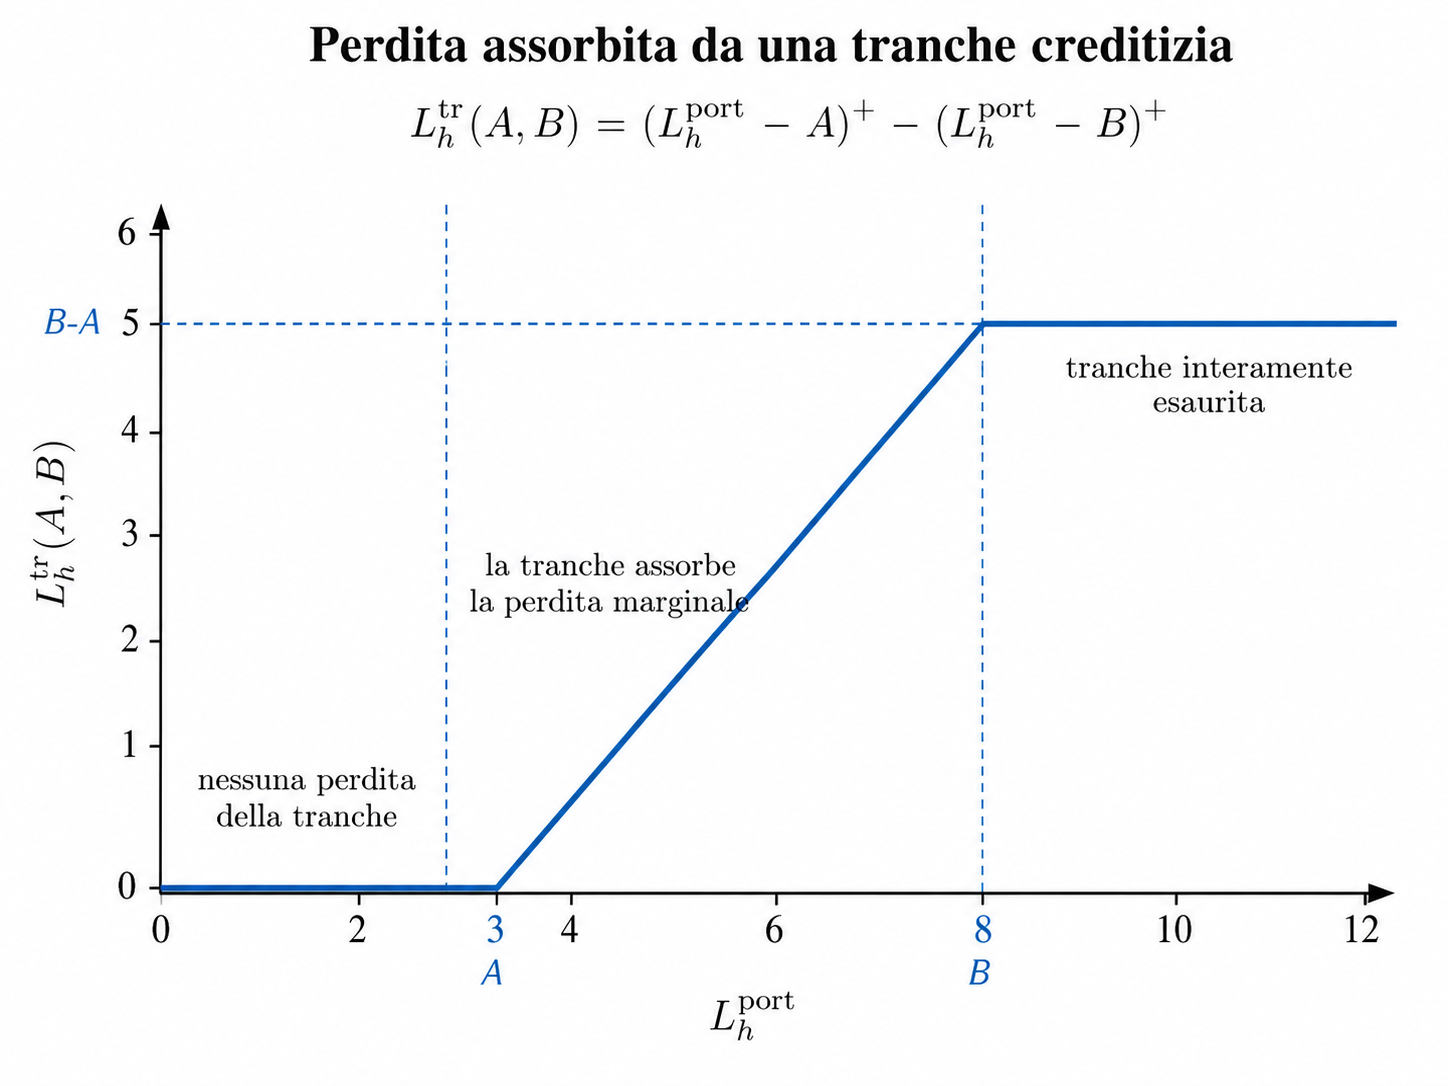
\includegraphics[width=0.82\textwidth]
{../graphics/Cap09_tranche_creditizia.png}
\caption{Profilo della perdita assorbita da una tranche creditizia con
attachment point $A$ e detachment point $B$.}
\label{fig:cap09-tranche-creditizia}
\end{figure}

La tranche non subisce perdite finch\'{e}

\[
L_h^{\mathrm{port}}\leq A.
\]

Per

\[
A<L_h^{\mathrm{port}}<B,
\]

la perdita della tranche cresce nella stessa misura della perdita
aggregata eccedente l'attachment point. Infine, quando

\[
L_h^{\mathrm{port}}\geq B,
\]

la tranche risulta interamente esaurita e la sua perdita raggiunge il
valore massimo

\[
B-A.
\]



La tranche non subisce perdite finch\'{e} la perdita aggregata rimane
inferiore ad $A$. Assorbe le perdite comprese tra $A$ e $B$ ed
\`{e} interamente esaurita quando

\[
L_h^{\mathrm{port}}\geq B.
\]

Per descrivere i flussi associati alla tranche occorre quindi
conoscere la distribuzione della perdita aggregata del portafoglio.
La dipendenza tra i default, influenzando la frequenza e la
concentrazione delle perdite elevate, diventa pertanto un elemento
essenziale.

Il pricing dei derivati multi-name non viene sviluppato nel presente
corso. Questi strumenti mostrano tuttavia perch\'{e} la modellizzazione
della dipendenza sia indispensabile: lo stesso insieme di probabilit\`{a}
marginali pu\`{o} generare valori e distribuzioni di perdita molto
differenti al variare della struttura congiunta.

\subsection{Raccordo con la Lezione 10}

\label{subsec:cap9-raccordo-lezione10}

Per un portafoglio con molti emittenti, la costruzione analitica della
distribuzione congiunta pu\`{o} diventare rapidamente complessa. La
Lezione~10 utilizzer\`{a} la simulazione per generare scenari congiunti
dei rating e delle perdite.

La struttura dell'applicazione sar\`{a}

\[
\boxed{
\begin{array}{c}
\text{transizioni individuali}
\\
+
\\
\text{dipendenza e fattori comuni}
\\
+
\\
\mathrm{LGD}\text{ ed }\mathrm{EAD}
\\
\downarrow
\\
\text{distribuzione simulata della perdita di portafoglio}.
\end{array}
}
\]

In ciascuno scenario simulato si proceder\`{a} a:

\begin{enumerate}

\item generare lo stato del fattore macroeconomico comune;

\item simulare le transizioni dei singoli emittenti condizionatamente
al fattore comune e ai rating iniziali;

\item associare a ogni stato futuro una perdita dipendente da
$\mathrm{LGD}$, $\mathrm{EAD}$ e dalla variazione di valore
dell'esposizione;

\item aggregare le perdite individuali:

\[
L_h^{\mathrm{port}}
=
\sum_{n=1}^{N}L_{n,h};
\]

\item ripetere la simulazione per ottenere una distribuzione empirica
della perdita aggregata;

\item stimare perdita attesa, varianza, VaR e CVaR del portafoglio.

\end{enumerate}

La Lezione~10 mostrer\`{a} quindi il passaggio operativo dalle matrici
marginali di transizione a una distribuzione di portafoglio nella quale
la dipendenza viene specificata e simulata esplicitamente.

\section{Impiego gestionale e regolamentare delle misure}

\label{sec:cap9-impiego-gestionale-regolamentare}

Le misure introdotte nel capitolo trovano applicazione nella gestione
del rischio, nella redazione del bilancio e nella valutazione
dell'adeguatezza patrimoniale. I diversi ambiti utilizzano concetti
collegati, ma non coincidenti.

In particolare, occorre distinguere tra:

\begin{itemize}
\item la perdita attesa;
\item gli accantonamenti contabili;
\item il capitale economico;
\item i requisiti patrimoniali prudenziali.
\end{itemize}

La presente sezione fornisce soltanto un inquadramento professionale.
La disciplina contabile e prudenziale completa viene rinviata agli
insegnamenti specialistici.

\subsection{Accantonamenti e IFRS 9}

\label{subsec:cap9-ifrs9}

Il principio contabile IFRS~9 adotta un modello fondato sulle
\emph{expected credit losses}, indicate con ECL. L'accantonamento
contabile dipende dall'evoluzione del rischio creditizio dello
strumento rispetto alla data della sua rilevazione iniziale.

L'IFRS~9 distingue due basi di misurazione delle perdite attese:

\begin{itemize}

\item l'\emph{expected credit loss a 12 mesi};

\item la \emph{lifetime expected credit loss}.

\end{itemize}

La differenza riguarda l'orizzonte entro il quale pu\`{o} verificarsi
il default. L'ECL a 12 mesi considera le perdite lungo la vita residua
dello strumento generate da eventi di default possibili nei dodici
mesi successivi. La lifetime ECL considera invece le perdite generate
da tutti i default possibili durante l'intera vita residua.

Quando si verifica un incremento significativo del rischio creditizio,
l'accantonamento viene invece determinato sulla base della
\emph{lifetime expected credit loss}, che considera gli eventi di
default possibili lungo l'intera vita residua dello strumento.

In forma schematica,

\[
\begin{array}{ccl}
\text{assenza di incremento significativo}
&
\longrightarrow
&
\text{ECL a 12 mesi},
\\[2mm]
\text{incremento significativo del rischio}
&
\longrightarrow
&
\text{lifetime ECL}.
\end{array}
\]

La valutazione dell'incremento significativo del rischio creditizio
richiede il confronto tra il rischio di default alla data corrente e
quello esistente al momento della rilevazione iniziale. Non coincide
quindi con la sola osservazione del rating corrente o con il
verificarsi del default.

Il modello markoviano sviluppato nel capitolo consente di rappresentare
in modo semplificato il collegamento tra transizioni dei rating e
lifetime ECL. Utilizzando una matrice di transizione predittiva
$P^{\Prob}$, le probabilit\`{a} marginali di default sono

\[
\mathrm{PD}_{i}^{\mathrm{marg}}(h)
=
\left[
\left(P^{\Prob}\right)^h
\right]_{iD}
-
\left[
\left(P^{\Prob}\right)^{h-1}
\right]_{iD}.
\]

In un modello discreto semplificato, definiamo la perdita creditizia
attualizzata lungo la vita residua come

\[
L_i^{\mathrm{life}}
=
\sum_{h=1}^{H}
d_h
\mathrm{LGD}_h
\mathrm{EAD}_h
\1_{\{\tau_D=h\}}.
\]

Se il default avviene alla data $h$, soltanto l'indicatrice
$\1_{\{\tau_D=h\}}$ assume valore uno. Se invece $\tau_D>H$, tutte le
indicatrici sono nulle e la perdita da default \`{e} pari a zero.
La lifetime expected credit loss \`{e} quindi il valore atteso della
perdita lungo la vita residua:

\[
\begin{split}
\mathrm{ECL}_{i}^{\mathrm{life}}
&=
\E^{\Prob}
\left[
L_i^{\mathrm{life}}
\mid X_0=i
\right]
\\
&=
\sum_{h=1}^{H}
d_h
\mathrm{PD}_{i}^{\mathrm{marg}}(h)
\mathrm{LGD}_h
\mathrm{EAD}_h.
\end{split}
\]
Il collegamento concettuale \`{e} quindi

\[
\boxed{
\left(P^{\Prob}\right)^h
\longrightarrow
\text{term structure delle probabilit\`{a} di default}
\longrightarrow
\text{lifetime ECL}.
}
\]

Nel modello annuale semplificato, l'ECL a 12 mesi utilizza la
probabilit\`{a} degli eventi di default che possono verificarsi nel
primo anno:

\[
\mathrm{ECL}_{i}^{12\mathrm{m}}
=
d_1
\mathrm{PD}_{i}^{\mathrm{marg}}(1)
\mathrm{LGD}_1
\mathrm{EAD}_1.
\]

Le formule precedenti costituiscono una rappresentazione didattica:
l'IFRS~9 non prescrive l'impiego di una matrice di transizione.

Nel modello qui adottato, la matrice $P^{\Prob}$ viene utilizzata per
ottenere probabilit\`{a} di default predittive. Una matrice stimata
sulle transizioni storiche pu\`{o} costituire il punto di partenza, ma
le probabilit\`{a} utilizzate nel calcolo dell'ECL devono riflettere
anche le condizioni correnti e le previsioni ragionevoli
sull'evoluzione futura dell'economia.

Si tratta pertanto di probabilit\`{a} sotto la misura fisica, finalizzate
alla previsione delle perdite, e non di probabilit\`{a} risk-neutral
utilizzate per il pricing.

\subsection{Capitale economico e capitale prudenziale}

\label{subsec:cap9-capitale-economico-prudenziale}

La perdita attesa, l'accantonamento contabile, il capitale economico
e il requisito patrimoniale prudenziale sono concetti collegati, ma
rispondono a finalit\`{a} differenti.

La \emph{perdita attesa} (\emph{Expected Loss}, \emph{EL}) \`{e} il
valore medio della variabile casuale perdita sotto la distribuzione
predittiva adottata:

\[
\mathrm{EL}
=
\E^{\Prob}[L].
\]

Essa rappresenta la perdita media associata all'esposizione o al
portafoglio nel modello considerato.

L'\emph{accantonamento contabile per perdite}
(\emph{loss allowance}) \`{e} invece l'importo rilevato in bilancio
a fronte delle perdite creditizie attese. Nell'IFRS~9 esso viene
misurato mediante le \emph{Expected Credit Losses} (\emph{ECL}),
utilizzando, a seconda dell'evoluzione del rischio creditizio, l'ECL
a 12 mesi oppure la lifetime ECL.

L'accantonamento contabile \`{e} quindi collegato alla perdita attesa,
ma non coincide necessariamente con la quantit\`{a} $\mathrm{EL}$
calcolata mediante un generico modello interno. La sua determinazione
dipende dalle regole contabili applicabili, dall'orizzonte considerato,
dall'attualizzazione e dalle informazioni previsionali utilizzate.

Il \emph{capitale economico} (\emph{Economic Capital}, \emph{EC})
\`{e} una misura gestionale interna delle risorse destinate ad
assorbire le perdite superiori alla perdita attesa, entro un
determinato orizzonte e livello di confidenza $\alpha$.

Secondo la convenzione adottata nel capitolo,

\[
\mathrm{EC}_{\alpha}
=
\VaR_{\alpha}(L)
-
\mathrm{EL},
\]

dove il \emph{Value at Risk} (\emph{VaR}) rappresenta il quantile
della perdita totale al livello di confidenza $\alpha$.

Il \emph{requisito patrimoniale prudenziale}
(\emph{prudential capital requirement}) \`{e} invece il capitale
richiesto dalle regole di vigilanza. Esso dipende, tra gli altri
elementi, dalle esposizioni, dalle ponderazioni per il rischio, dai
parametri regolamentari, dal metodo di calcolo applicato e dagli
eventuali requisiti o riserve aggiuntivi previsti dal quadro
prudenziale.

Le quattro nozioni possono essere sintetizzate come segue:

\[
\begin{array}{p{4.2cm}p{7.4cm}}
\hline
\textbf{Concetto}
&
\textbf{Funzione principale}
\\
\hline
\emph{Expected Loss} (\emph{EL})
&
misurare la perdita media prodotta dal modello probabilistico;
\\
\emph{loss allowance}
&
rilevare in bilancio le perdite creditizie attese misurate mediante
le \emph{ECL};
\\
\emph{Economic Capital} (\emph{EC})
&
determinare internamente le risorse destinate ad assorbire le perdite
superiori alla perdita attesa;
\\
\emph{prudential capital requirement}
&
determinare il capitale richiesto dalle regole di vigilanza.
\\
\hline
\end{array}
\]

La relazione

\[
\mathrm{EC}_{\alpha}
=
\VaR_{\alpha}(L)
-
\mathrm{EL}
\]

costituisce pertanto una convenzione gestionale per il calcolo del
capitale economico. Non rappresenta una formula generale per la
determinazione del requisito patrimoniale prudenziale.

\subsection{Stress testing}

\label{subsec:cap9-stress-testing}

Il VaR e il CVaR sono misure probabilistiche ricavate da una
distribuzione stimata delle perdite:

\[
F_L
\longrightarrow
\VaR_{\alpha}(L),
\qquad
\CVaR_{\alpha}(L).
\]

I risultati dipendono quindi dal modello adottato, dai dati utilizzati,
dalla struttura di dipendenza e dalle ipotesi formulate sulle
transizioni, sulle esposizioni e sui tassi di recupero.

Lo stress testing segue una logica differente. Si specifica uno
scenario avverso, ad esempio una recessione, un aumento dei default,
una riduzione dei recovery rate o un deterioramento simultaneo di
determinati settori, e si valuta la perdita che ne deriverebbe.

Indicando con $z^{\mathrm{stress}}$ lo scenario avverso assegnato, si
considera una quantit\`{a} del tipo

\[
L^{\mathrm{stress}}
=
L\left(z^{\mathrm{stress}}\right).
\]

Lo scenario di stress non deve necessariamente essere identificato
con un quantile della distribuzione stimata, n\'{e} deve essergli
attribuita una probabilit\`{a} precisa. La sua funzione \`{e} valutare
la vulnerabilit\`{a} della posizione o del portafoglio rispetto a una
configurazione avversa specifica.

Le due prospettive sono complementari:

\[
\boxed{
\begin{array}{c}
\text{misure probabilistiche}
\quad+\quad
\text{scenari di stress}
\\[-0.5mm]
\longrightarrow
\quad
\text{valutazione pi\`{u} completa del rischio}
\end{array}
}
\]

Il VaR e il CVaR sintetizzano la distribuzione prodotta dal modello; lo
stress testing verifica invece le conseguenze di scenari avversi che
possono risultare particolarmente rilevanti dal punto di vista
gestionale o prudenziale.

\section{Limiti del modello e rischio di modello}

\label{sec:cap9-limiti-rischio-modello}

Le misure di rischio ottenute nel capitolo non sono quantit\`{a}
direttamente osservabili. Esse sono il risultato di una successione di
scelte modellistiche che riguardano la dinamica dei rating, la
traduzione degli stati futuri in perdite e, nel caso di un portafoglio,
la dipendenza tra gli emittenti.

Nel presente capitolo, con \emph{rischio di modello}
(\emph{model risk}) si indica il rischio che una rappresentazione
incompleta, non adeguatamente specificata o non correttamente calibrata
produca stime delle perdite e delle misure di rischio non sufficientemente
affidabili.

I limiti del modello vengono quindi organizzati secondo le principali
componenti della catena di misurazione.

\subsection{Modello delle transizioni}

\label{subsec:cap9-limiti-transizioni}

Il modello delle transizioni determina le probabilit\`{a} associate ai
rating futuri e al default. Le sue conclusioni dipendono dalla validit\`{a}
della struttura markoviana e dalla capacit\`{a} della matrice di
transizione di rappresentare l'evoluzione futura del rischio creditizio.

\paragraph{Validit\`{a} della propriet\`{a} di Markov.}

La propriet\`{a} di Markov assume che, condizionatamente al rating
corrente, la distribuzione del rating futuro non dipenda ulteriormente
dalla storia precedente dell'emittente.

Questa ipotesi pu\`{o} risultare restrittiva. Due emittenti collocati
nella stessa classe di rating possono avere prospettive differenti se
uno vi permane da diversi anni, mentre l'altro vi \`{e} appena entrato
in seguito a un downgrade. La durata della permanenza nello stato, la
direzione delle precedenti migrazioni e altre informazioni storiche
possono quindi contenere capacit\`{a} predittiva non rappresentata dal
solo rating corrente.

In questi casi, il modello pu\`{o} essere ampliato introducendo ulteriori
variabili di stato oppure adottando una dinamica non strettamente
markoviana.

\paragraph{Omogeneit\`{a} temporale.}

Nel modello omogeneo, una sola matrice $P$ descrive le probabilit\`{a}
di transizione in ogni periodo. La distribuzione a $h$ periodi viene
pertanto ottenuta mediante

\[
P^h.
\]

Questa rappresentazione presuppone che le probabilit\`{a} di upgrade,
downgrade e default restino costanti nel tempo. Tale ipotesi pu\`{o}
essere poco realistica quando il rischio creditizio varia con il ciclo
economico, con le condizioni finanziarie o con eventi settoriali.

Se la matrice dipende dal tempo, la probabilit\`{a} di transizione tra
le date $t$ e $t+h$ non \`{e} descritta da $P^h$, ma dal prodotto

\[
P_t P_{t+1}\cdots P_{t+h-1}.
\]

L'impiego di una matrice omogenea costituisce quindi una
semplificazione la cui adeguatezza dipende dall'orizzonte e dal
contesto applicativo.

\paragraph{Qualit\`{a} della classificazione dei rating.}

Il rating deve sintetizzare le informazioni rilevanti per prevedere
l'evoluzione del merito creditizio. Se le classi sono troppo ampie,
emittenti sostanzialmente differenti vengono trattati come se avessero
la stessa distribuzione futura.

Anche errori di classificazione, cambiamenti nei criteri di assegnazione
dei rating o differenze tra sistemi interni ed esterni modificano le
frequenze di transizione osservate. La matrice pu\`{o} quindi riflettere
non soltanto l'evoluzione del rischio degli emittenti, ma anche le
caratteristiche del sistema di classificazione utilizzato.

\paragraph{Rotture strutturali.}

Una matrice stimata sui dati passati pu\`{o} perdere capacit\`{a}
predittiva quando cambiano stabilmente le condizioni economiche o
istituzionali. Crisi finanziarie, modifiche normative, innovazioni nei
processi di concessione del credito o trasformazioni strutturali di un
settore possono produrre probabilit\`{a} di transizione differenti da
quelle osservate nel campione storico.

L'uso meccanico di una matrice storica presuppone quindi una stabilit\`{a}
che deve essere valutata e non semplicemente assunta.

\subsection{Modello delle perdite}

\label{subsec:cap9-limiti-perdite}

La matrice di transizione assegna probabilit\`{a} agli stati futuri,
ma non determina da sola la distribuzione delle perdite. Occorre anche
specificare la funzione di perdita

\[
\ell(j,h),
\]

che associa a ciascuno stato futuro $j$ la corrispondente conseguenza
economica. Come definito in precedenza,

\[
L_h=\ell(X_h,h).
\]

Nel modello mark-to-market adottato nel capitolo, tale funzione viene
costruita confrontando il valore dell'esposizione nello stato futuro
con il valore di riferimento:

\[
\ell(j,h)
=
V^{\mathrm{ref}}(h)-V_j(h).
\]

Anche questa trasformazione introduce ipotesi e fonti di rischio di
modello.

\paragraph{Incertezza dell'\emph{Exposure at Default} (\emph{EAD}).}

L'\emph{EAD} rappresenta l'esposizione esistente nel momento in cui si
verifica il default. Essa non coincide necessariamente con
l'esposizione osservata alla data iniziale.

Rimborsi, nuove erogazioni, utilizzi di linee di credito e variazioni
delle garanzie possono modificare l'importo effettivamente esposto. Il
trattamento dell'\emph{EAD} come quantit\`{a} deterministica trascura
questa fonte di incertezza.

\paragraph{Aleatoriet\`{a} della \emph{Loss Given Default} (\emph{LGD}).}

La \emph{LGD} misura la quota dell'esposizione che non viene recuperata
in caso di default. Essa dipende, tra gli altri elementi, dalle
garanzie disponibili, dal grado di subordinazione, dai tempi di
recupero e dai costi delle procedure.

Una rappresentazione semplificata pu\`{o} utilizzare un unico valore di
$\mathrm{LGD}$. In realt\`{a}, anche condizionatamente al default, la
perdita pu\`{o} essere aleatoria:

\[
L_h^{\mathrm{def}}
=
\mathrm{EAD}_h
\mathrm{LGD}_h
\1_{\{\tau_D=h\}}.
\]

La sostituzione di $\mathrm{EAD}_h$ e $\mathrm{LGD}_h$ con valori
deterministici riduce la variabilit\`{a} rappresentata dal modello e
pu\`{o} sottostimare la dispersione delle perdite.

\paragraph{Dipendenza dei recuperi dal ciclo economico.}

I tassi di recupero possono deteriorarsi proprio nelle fasi in cui
aumentano i default. Durante una recessione, il numero di attivit\`{a}
da liquidare pu\`{o} crescere, mentre il valore delle garanzie e la
capacit\`{a} del mercato di assorbirle possono diminuire.

Assumere una \emph{LGD} costante e indipendente dalle transizioni
creditizie elimina questa possibile relazione tra frequenza dei
default e severit\`{a} delle perdite.

\paragraph{Spread e valori associati ai rating.}

Nel modello mark-to-market, a ciascun rating viene associato uno spread
e, attraverso lo spread, un valore dello strumento. La relazione

\[
j
\longmapsto
s_j
\longmapsto
V_j(h)
\]

costituisce una componente autonoma del modello.

Emittenti appartenenti alla stessa classe possono presentare spread
differenti per effetto della liquidit\`{a}, della durata, del settore,
della struttura contrattuale e delle condizioni di mercato. Associare
un solo valore a ogni rating comprime questa eterogeneit\`{a} e rende
la perdita dipendente dalla specifica tabella di spread adottata.

\paragraph{Scelta del valore di riferimento.}

La perdita dipende anche dal valore di riferimento
$V^{\mathrm{ref}}(h)$. Il valore nominale, il valore contabile, il
valore iniziale e il valore che lo strumento avrebbe mantenendo il
rating corrente rispondono a domande differenti.

Due modelli che utilizzano le stesse probabilit\`{a} di transizione e
gli stessi valori futuri possono quindi produrre perdite differenti
se adottano valori di riferimento diversi. La scelta deve essere
coerente con la finalit\`{a} della misurazione e dichiarata
esplicitamente.

\subsection{Modello di portafoglio}

\label{subsec:cap9-limiti-portafoglio}

Per un portafoglio di $N$ esposizioni, la perdita aggregata \`{e}

\[
L_h^{\mathrm{port}}
=
\sum_{n=1}^{N}L_{n,h}.
\]

Le distribuzioni individuali delle perdite non sono tuttavia
sufficienti per determinare la distribuzione della somma. Occorre
specificare la dipendenza tra i rating futuri e tra i default dei
diversi emittenti.

\paragraph{Dipendenza tra debitori.}

Le matrici di transizione dei singoli emittenti determinano le
rispettive distribuzioni individuali, ma non determinano la
distribuzione congiunta del vettore dei rating futuri.

Modelli con le stesse probabilit\`{a} individuali di default possono
produrre probabilit\`{a} molto differenti di default simultanei. Di
conseguenza, possono generare distribuzioni di perdita, VaR e CVaR
sensibilmente differenti.

\paragraph{Concentrazione.}

La concentrazione nasce quando una parte rilevante del portafoglio
dipende da pochi debitori, settori, aree geografiche o tipologie di
garanzia. In questi casi, anche un singolo evento negativo pu\`{o}
produrre una perdita elevata.

Un modello che rappresenta correttamente le probabilit\`{a} di default,
ma trascura la distribuzione delle esposizioni, pu\`{o} sottovalutare il
rischio complessivo del portafoglio.

\paragraph{Fattori comuni.}

I debitori possono essere influenzati dagli stessi fattori
macroeconomici e finanziari, come crescita economica, tassi di
interesse, prezzi delle materie prime o condizioni di liquidit\`{a}.

L'introduzione di fattori comuni consente di rappresentare il fatto che
le transizioni peggiorative tendono a concentrarsi negli stessi
scenari. La specificazione e la calibrazione di tali fattori incidono
direttamente sulla probabilit\`{a} di perdite aggregate elevate.

\paragraph{Rischio sistematico.}

La diversificazione pu\`{o} ridurre la componente idiosincratica del
rischio, ma non elimina gli effetti degli shock comuni. Il rischio
sistematico produce dipendenza tra i debitori e pu\`{o} generare
concentrazioni di default proprio nelle fasi economiche avverse.

La varianza della perdita di portafoglio evidenzia il ruolo delle
covarianze:

\[
\Var
\left(
L_h^{\mathrm{port}}
\right)
=
\sum_{n=1}^{N}
\Var(L_{n,h})
+
2
\sum_{n<m}
\Cov(L_{n,h},L_{m,h}).
\]

Per le misure di coda, la sola conoscenza delle covarianze non \`{e}
generalmente sufficiente: assumono rilievo anche la forma della
dipendenza e la probabilit\`{a} di perdite estreme congiunte.

\subsection{Modello di pricing e copertura}

\label{subsec:cap9-limiti-pricing-copertura}

La valutazione e la copertura mediante \emph{Credit Default Swap}
(\emph{CDS}) introducono ulteriori componenti di rischio di modello.
Una copertura contrattualmente collegata al default non elimina
necessariamente tutte le fonti di perdita economica.

\paragraph{Differenza tra misura fisica e misura risk-neutral.}

La matrice $P^{\Prob}$ descrive una distribuzione predittiva e viene
utilizzata per misurare il rischio. La matrice $P^{\Q}$ viene invece
utilizzata per valutare flussi finanziari coerentemente con i prezzi di
mercato.

Le due matrici rispondono a finalit\`{a} differenti e non sono
generalmente intercambiabili. L'impiego di probabilit\`{a} fisiche nel
pricing o di probabilit\`{a} risk-neutral nella previsione delle
frequenze di default pu\`{o} produrre risultati privi di una chiara
interpretazione economica.

\paragraph{Calibrazione della matrice risk-neutral.}

La matrice $P^{\Q}$ non viene normalmente osservata in modo diretto.
Essa deve essere calibrata utilizzando prezzi o spread di strumenti
negoziati e ipotesi sui tassi di recupero, sull'attualizzazione e sui
premi per il rischio.

Strumenti di mercato limitati o poco liquidi possono non identificare
univocamente tutte le probabilit\`{a} di transizione risk-neutral.
Matrici differenti possono quindi risultare compatibili con gli stessi
prezzi osservati, ma produrre valutazioni differenti per strumenti non
utilizzati nella calibrazione.

\paragraph{Rischio di controparte.}

La protezione acquistata mediante un \emph{CDS} dipende dalla
capacit\`{a} del protection seller di effettuare il pagamento previsto
in caso di evento creditizio. Il valore della copertura non dipende
quindi soltanto dal rischio dell'entit\`{a} di riferimento, ma anche dal
rischio di default della controparte del contratto.

Trattare il pagamento del \emph{CDS} come certo pu\`{o} sovrastimare
l'efficacia della copertura.

\paragraph{\emph{Basis risk}.}

Il \emph{basis risk} nasce quando l'esposizione da coprire e il
contratto di copertura non coincidono perfettamente. Le differenze
possono riguardare l'entit\`{a} di riferimento, la scadenza, il valore
nozionale, la valuta, la seniority o la definizione contrattuale
dell'evento creditizio.

In presenza di tali differenze, la perdita sull'esposizione e il
pagamento del \emph{CDS} possono non compensarsi integralmente.

\paragraph{Liquidit\`{a} del mercato dei CDS.}

Gli spread osservati possono dipendere anche dalla liquidit\`{a} dello
strumento e non soltanto dal rischio di credito. Inoltre, una posizione
di copertura pu\`{o} risultare costosa da modificare o chiudere quando
il mercato \`{e} poco liquido.

Un modello basato su spread teorici e transazioni prive di costi pu\`{o}
quindi sovrastimare la possibilit\`{a} di costruire o ribilanciare la
copertura alle condizioni previste.

\subsection{Conclusione: propagazione del rischio di modello}

\label{subsec:cap9-conclusione-rischio-modello}

Il rischio di modello non riguarda una sola formula finale. Esso si
propaga lungo l'intera catena di misurazione.

Il modello delle transizioni determina le probabilit\`{a} degli stati
futuri. Il modello dei valori e dei recuperi trasforma tali stati in
perdite. Il modello di dipendenza combina infine le perdite individuali
nella distribuzione della perdita di portafoglio.

\[
\boxed{
\begin{array}{c}
\text{modello delle transizioni}
\\[1mm]
+
\\[-1mm]
\text{modello dei valori e dei recuperi}
\\[1mm]
+
\\[-1mm]
\text{modello di dipendenza}
\\[2mm]
\downarrow
\\[2mm]
\text{distribuzione delle perdite}
\\
\text{e misure di rischio}
\end{array}
}
\]

VaR, CVaR, perdita attesa e capitale economico dipendono quindi
congiuntamente dalle tre componenti. Una maggiore precisione in una
sola parte della catena non compensa necessariamente una
specificazione inadeguata delle altre.

Nel caso del pricing e della copertura, a questi elementi si aggiungono
la scelta della misura di probabilit\`{a}, la calibrazione
risk-neutral e le imperfezioni del contratto e del mercato.

\section{Esercizi svolti}

\label{sec:cap09-esercizi-svolti}

\begin{exercise}[Term structure delle probabilit\`{a} di default]

\label{ex:cap09-term-structure-default}

Si consideri una catena di Markov con spazio degli stati

\[
\mathcal{I}=\{1,2,3,D\},
\]

dove $D$ rappresenta il default ed \`{e} uno stato assorbente. La
matrice annuale di transizione sotto la misura fisica \`{e}

\[
P^{\Prob}
=
\begin{pmatrix}
0.86 & 0.11 & 0.02 & 0.01\\
0.05 & 0.78 & 0.14 & 0.03\\
0.01 & 0.09 & 0.72 & 0.18\\
0    & 0    & 0    & 1
\end{pmatrix}.
\]

Alla data iniziale l'emittente si trova nello stato $X_0=2$. Si
indichi con

\[
\tau_D
=
\inf\{h\geq 1:X_h=D\}
\]

il primo istante di ingresso in default e si consideri un orizzonte
di cinque anni.

\begin{enumerate}

\item Calcolare la distribuzione di $X_h$, condizionatamente a $X_0=2$,
per $h=1,\ldots,5$.

\item Calcolare, per ogni $h=1,\ldots,5$:

\begin{itemize}

\item la probabilit\`{a} cumulativa di default
$\mathrm{PD}_{2}^{\mathrm{cum}}(h)$;

\item la probabilit\`{a} marginale di default
$\mathrm{PD}_{2}^{\mathrm{marg}}(h)$;

\item la probabilit\`{a} di sopravvivenza $S_2(h)$;

\item la probabilit\`{a} condizionata di default $q_2(h)$.

\end{itemize}

\item Verificare le relazioni tra probabilit\`{a} cumulativa,
probabilit\`{a} marginale, sopravvivenza e probabilit\`{a}
condizionata.

\item Interpretare l'evoluzione temporale delle quantit\`{a} ottenute.

\end{enumerate}

\end{exercise}

\noindent
\textbf{Soluzione.}

\begin{enumerate}

\item Poich\'{e} la catena \`{e} omogenea, la distribuzione del rating
alla data $h$, condizionatamente allo stato iniziale $X_0=2$, \`{e}
data dalla seconda riga di

\[
\left(P^{\Prob}\right)^h.
\]

Per abbreviare la notazione, poniamo

\[
p_{2j}^{(h)}
=
\Prob(X_h=j\mid X_0=2)
=
\left[
\left(P^{\Prob}\right)^h
\right]_{2j},
\qquad
j\in\mathcal{I}.
\]

Le distribuzioni ottenute sono quindi:

\[
\begin{array}{c|cccc}
h
&
p_{21}^{(h)}
&
p_{22}^{(h)}
&
p_{23}^{(h)}
&
p_{2D}^{(h)}
\\
\hline
1 & 0.050000 & 0.780000 & 0.140000 & 0.030000\\
2 & 0.083400 & 0.626500 & 0.211000 & 0.079100\\
3 & 0.105159 & 0.516834 & 0.241298 & 0.136709\\
4 & 0.118691 & 0.436415 & 0.248195 & 0.196699\\
5 & 0.126377 & 0.375797 & 0.242172 & 0.255654
\end{array}
\]
Ciascuna riga somma a uno e rappresenta la distribuzione del rating
alla corrispondente data futura.

\item Poich\'{e} il default \`{e} assorbente, la probabilit\`{a}
cumulativa di default coincide con la probabilit\`{a} di trovarsi
nello stato $D$ alla data $h$:

\[
\mathrm{PD}_{2}^{\mathrm{cum}}(h)
=
\Prob(\tau_D\leq h\mid X_0=2)
=
\left[
\left(P^{\Prob}\right)^h
\right]_{2D}.
\]

Ponendo

\[
\mathrm{PD}_{2}^{\mathrm{cum}}(0)=0,
\]

la probabilit\`{a} marginale di default \`{e}

\[
\begin{split}
\mathrm{PD}_{2}^{\mathrm{marg}}(h)
&=
\Prob(\tau_D=h\mid X_0=2)
\\
&=
\mathrm{PD}_{2}^{\mathrm{cum}}(h)
-
\mathrm{PD}_{2}^{\mathrm{cum}}(h-1).
\end{split}
\]

La probabilit\`{a} di sopravvivenza fino alla data $h$ \`{e}

\[
S_2(h)
=
\Prob(\tau_D>h\mid X_0=2)
=
1-\mathrm{PD}_{2}^{\mathrm{cum}}(h).
\]

Ponendo $S_2(0)=1$, la probabilit\`{a} condizionata di default nel
periodo $h$ \`{e}

\[
\begin{split}
q_2(h)
&=
\Prob
\left(
\tau_D=h
\mid
\tau_D>h-1,\ X_0=2
\right)
\\
&=
\frac{
\mathrm{PD}_{2}^{\mathrm{marg}}(h)
}{
S_2(h-1)
}.
\end{split}
\]

Si ottiene:

\[
\begin{array}{c|cccc}
h
&
\mathrm{PD}_{2}^{\mathrm{cum}}(h)
&
\mathrm{PD}_{2}^{\mathrm{marg}}(h)
&
S_2(h)
&
q_2(h)
\\
\hline
1 & 0.030000 & 0.030000 & 0.970000 & 0.030000\\
2 & 0.079100 & 0.049100 & 0.920900 & 0.050619\\
3 & 0.136709 & 0.057609 & 0.863291 & 0.062557\\
4 & 0.196699 & 0.059990 & 0.803301 & 0.069490\\
5 & 0.255654 & 0.058954 & 0.744346 & 0.073390
\end{array}
\]

Ad esempio, per il secondo anno,

\[
\mathrm{PD}_{2}^{\mathrm{marg}}(2)
=
0.079100-0.030000
=
0.049100,
\]

mentre

\[
q_2(2)
=
\frac{0.049100}{0.970000}
\approx
0.050619.
\]

La prima quantit\`{a} \`{e} una probabilit\`{a} non condizionata,
calcolata rispetto all'intera popolazione iniziale. La seconda \`{e}
invece la probabilit\`{a} di default nel secondo anno, condizionatamente
alla sopravvivenza durante il primo anno.

\item Per ogni $h$ vale anzitutto

\[
\mathrm{PD}_{2}^{\mathrm{cum}}(h)
+
S_2(h)
=
1.
\]

La probabilit\`{a} marginale pu\`{o} essere ricostruita dalla
probabilit\`{a} condizionata mediante

\[
\mathrm{PD}_{2}^{\mathrm{marg}}(h)
=
S_2(h-1)q_2(h).
\]

La probabilit\`{a} cumulativa \`{e} inoltre la somma delle
probabilit\`{a} marginali fino alla data considerata:

\[
\mathrm{PD}_{2}^{\mathrm{cum}}(h)
=
\sum_{k=1}^{h}
\mathrm{PD}_{2}^{\mathrm{marg}}(k).
\]

In particolare,

\[
\sum_{h=1}^{5}
\mathrm{PD}_{2}^{\mathrm{marg}}(h)
=
0.255654.
\]

La somma non \`{e} pari a uno, poich\'{e} rimane la probabilit\`{a}

\[
S_2(5)
=
0.744346
\]

che l'emittente non entri in default entro il quinto anno.

La Figura~\ref{fig:cap09-term-structure-default-esercizio} mostra
l'evoluzione della probabilit\`{a} cumulativa di default e della
corrispondente probabilit\`{a} di sopravvivenza.

\begin{figure}[htbp]
\centering
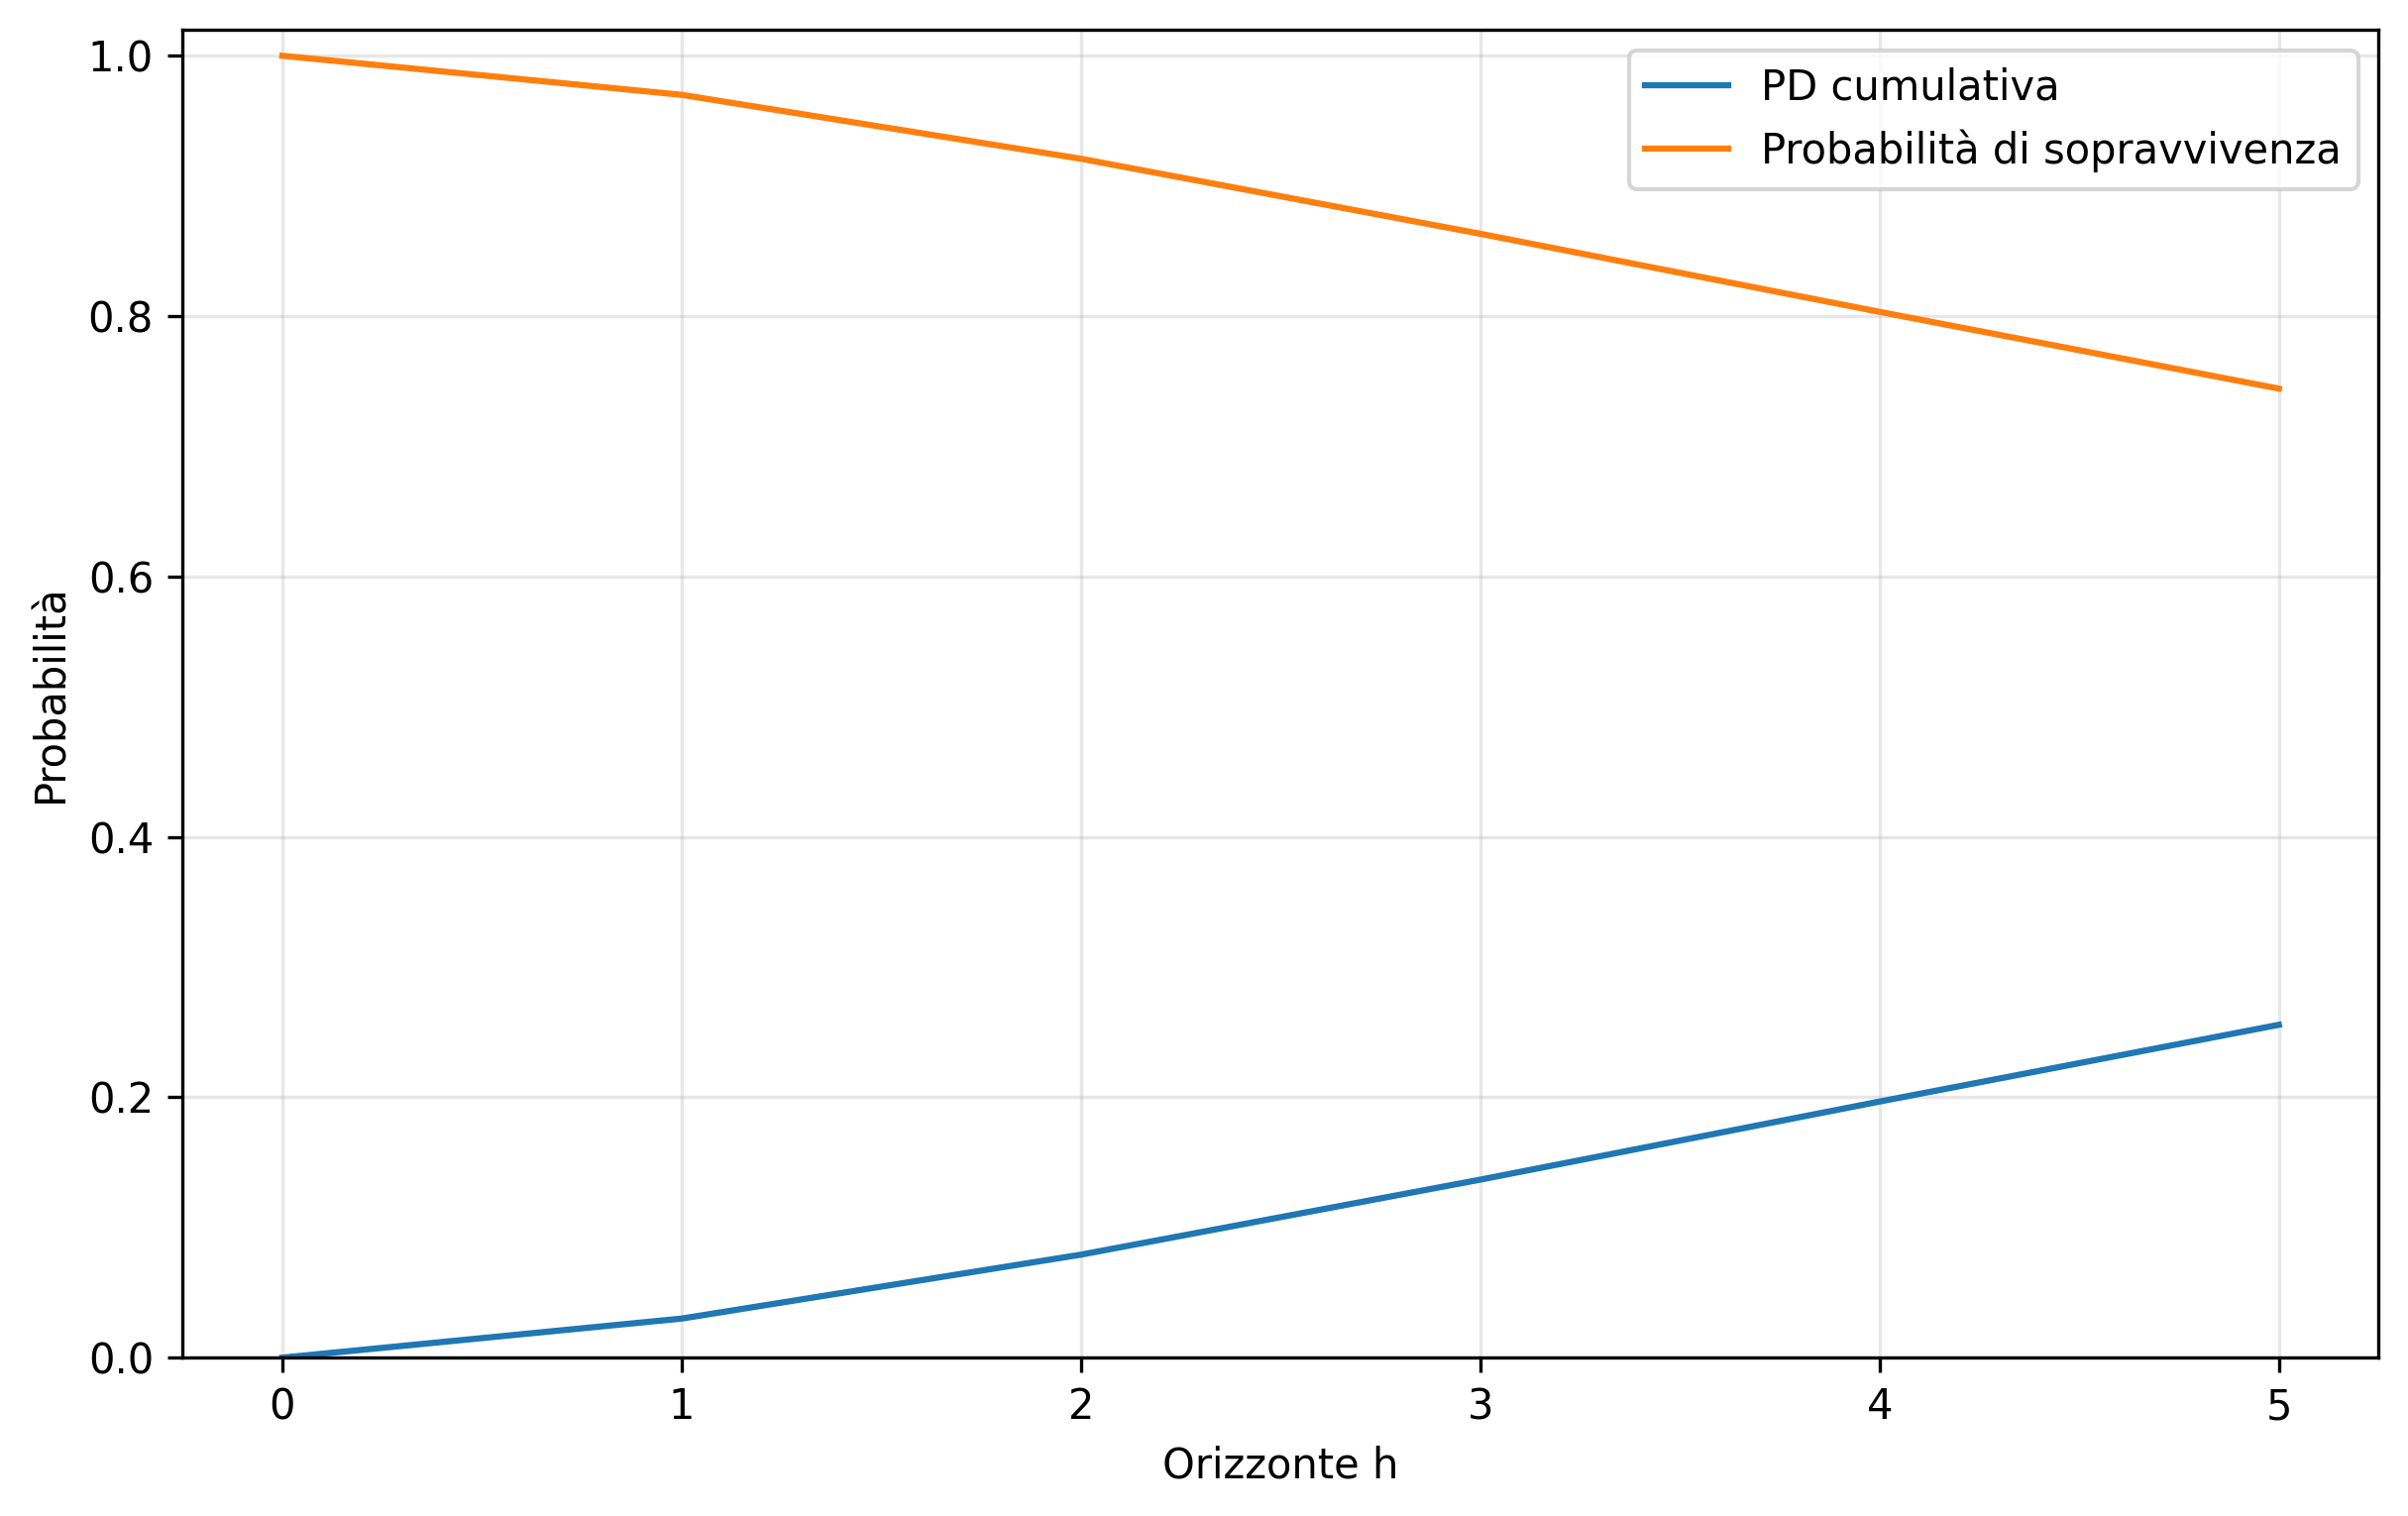
\includegraphics[width=0.78\textwidth]
{../graphics/Cap09_term_structure_default_esercizio.png}
\caption{Term structure della probabilit\`{a} cumulativa di default e
della probabilit\`{a} di sopravvivenza, condizionatamente al rating
iniziale $X_0=2$. Le due quantit\`{a} sono complementari a ogni
orizzonte.}
\label{fig:cap09-term-structure-default-esercizio}
\end{figure}

\item La probabilit\`{a} cumulativa di default cresce con l'orizzonte,
poich\'{e} incorpora tutti i possibili ingressi in default verificatisi
entro la data considerata. Simmetricamente, la probabilit\`{a} di
sopravvivenza diminuisce.

La probabilit\`{a} marginale misura invece il contributo del singolo
anno all'aumento della probabilit\`{a} cumulativa. Nel modello
considerato essa cresce nei primi quattro anni e si riduce lievemente
nel quinto.

La probabilit\`{a} condizionata di default aumenta dal $3\%$ del primo
anno a circa il $7.34\%$ del quinto anno. Il confronto con la
probabilit\`{a} marginale evidenzia l'effetto del condizionamento: il
rischio del singolo periodo viene misurato rispetto agli emittenti che
sono ancora sopravvissuti all'inizio del periodo stesso.

\end{enumerate}

\begin{exercise}[Distribuzione della perdita da migrazione]

\label{ex:cap09-distribuzione-perdita}

Si consideri un emittente inizialmente classificato nello stato
$X_0=2$. Dalla matrice di transizione dell'Esercizio precedente, la
distribuzione del rating dopo un anno \`{e}

\[
\begin{array}{c|cccc}
j & 1 & 2 & 3 & D\\
\hline
\Prob(X_1=j\mid X_0=2)
&
0.05
&
0.78
&
0.14
&
0.03
\end{array}
\]

Il valore di riferimento dell'esposizione alla data $h=1$ \`{e}

\[
V^{\mathrm{ref}}(h=1)=100.
\]

Ai quattro possibili rating futuri vengono associati i valori

\[
\begin{array}{c|cccc}
j & 1 & 2 & 3 & D\\
\hline
V_j(1)
&
104
&
100
&
90
&
45
\end{array}
\]

Si definisce la perdita a un anno mediante

\[
L_1=\ell(X_1,1),
\]

dove

\[
\ell(j,1)
=
V^{\mathrm{ref}}(1)-V_j(1).
\]

Condizionatamente al valore iniziale $X_0=2$:

\begin{enumerate}

\item Determinare la perdita associata a ciascun rating futuro.

\item Costruire la funzione di massa della variabile casuale $L_1$.

\item Determinare la funzione di ripartizione $F_{L_1}$.

\item Calcolare la perdita attesa.

\item Calcolare il momento secondo della perdita.

\item Calcolare la varianza e la deviazione standard.

\item Interpretare economicamente la distribuzione e i contributi dei
diversi stati alla perdita attesa.

\end{enumerate}

\end{exercise}

\noindent
\textbf{Soluzione.}

\begin{enumerate}

\item La funzione di perdita associa a ciascuno stato futuro la
differenza tra il valore di riferimento e il valore dell'esposizione
nello stato considerato:

\[
\ell(j,1)
=
V^{\mathrm{ref}}(1)-V_j(1).
\]

Si ottiene:

\[
\begin{array}{c|cccc}
j & 1 & 2 & 3 & D\\
\hline
V_j(1)
&
104
&
100
&
90
&
45
\\
\ell(j,1)
&
-4
&
0
&
10
&
55
\end{array}
\]

Pertanto,

\[
L_1
=
\begin{cases}
-4 & \text{se }X_1=1,\\
0  & \text{se }X_1=2,\\
10 & \text{se }X_1=3,\\
55 & \text{se }X_1=D.
\end{cases}
\]

La perdita negativa associata allo stato $1$ rappresenta un guadagno
rispetto al valore di riferimento: il miglioramento del rating
determina infatti un aumento del valore dell'esposizione.

\item La funzione di massa della perdita \`{e} ottenuta trasferendo le
probabilit\`{a} degli stati futuri sui corrispondenti valori di
perdita:

\[
\begin{array}{c|cccc}
\lambda
&
-4
&
0
&
10
&
55
\\
\hline
\Prob(L_1=\lambda\mid X_0=2)
&
0.05
&
0.78
&
0.14
&
0.03
\end{array}
\]

Le probabilit\`{a} sommano a uno:

\[
0.05+0.78+0.14+0.03=1.
\]

La Figura~\ref{fig:cap09-distribuzione-perdita-esercizio} rappresenta
la funzione di massa della perdita.

\begin{figure}[htbp]
\centering
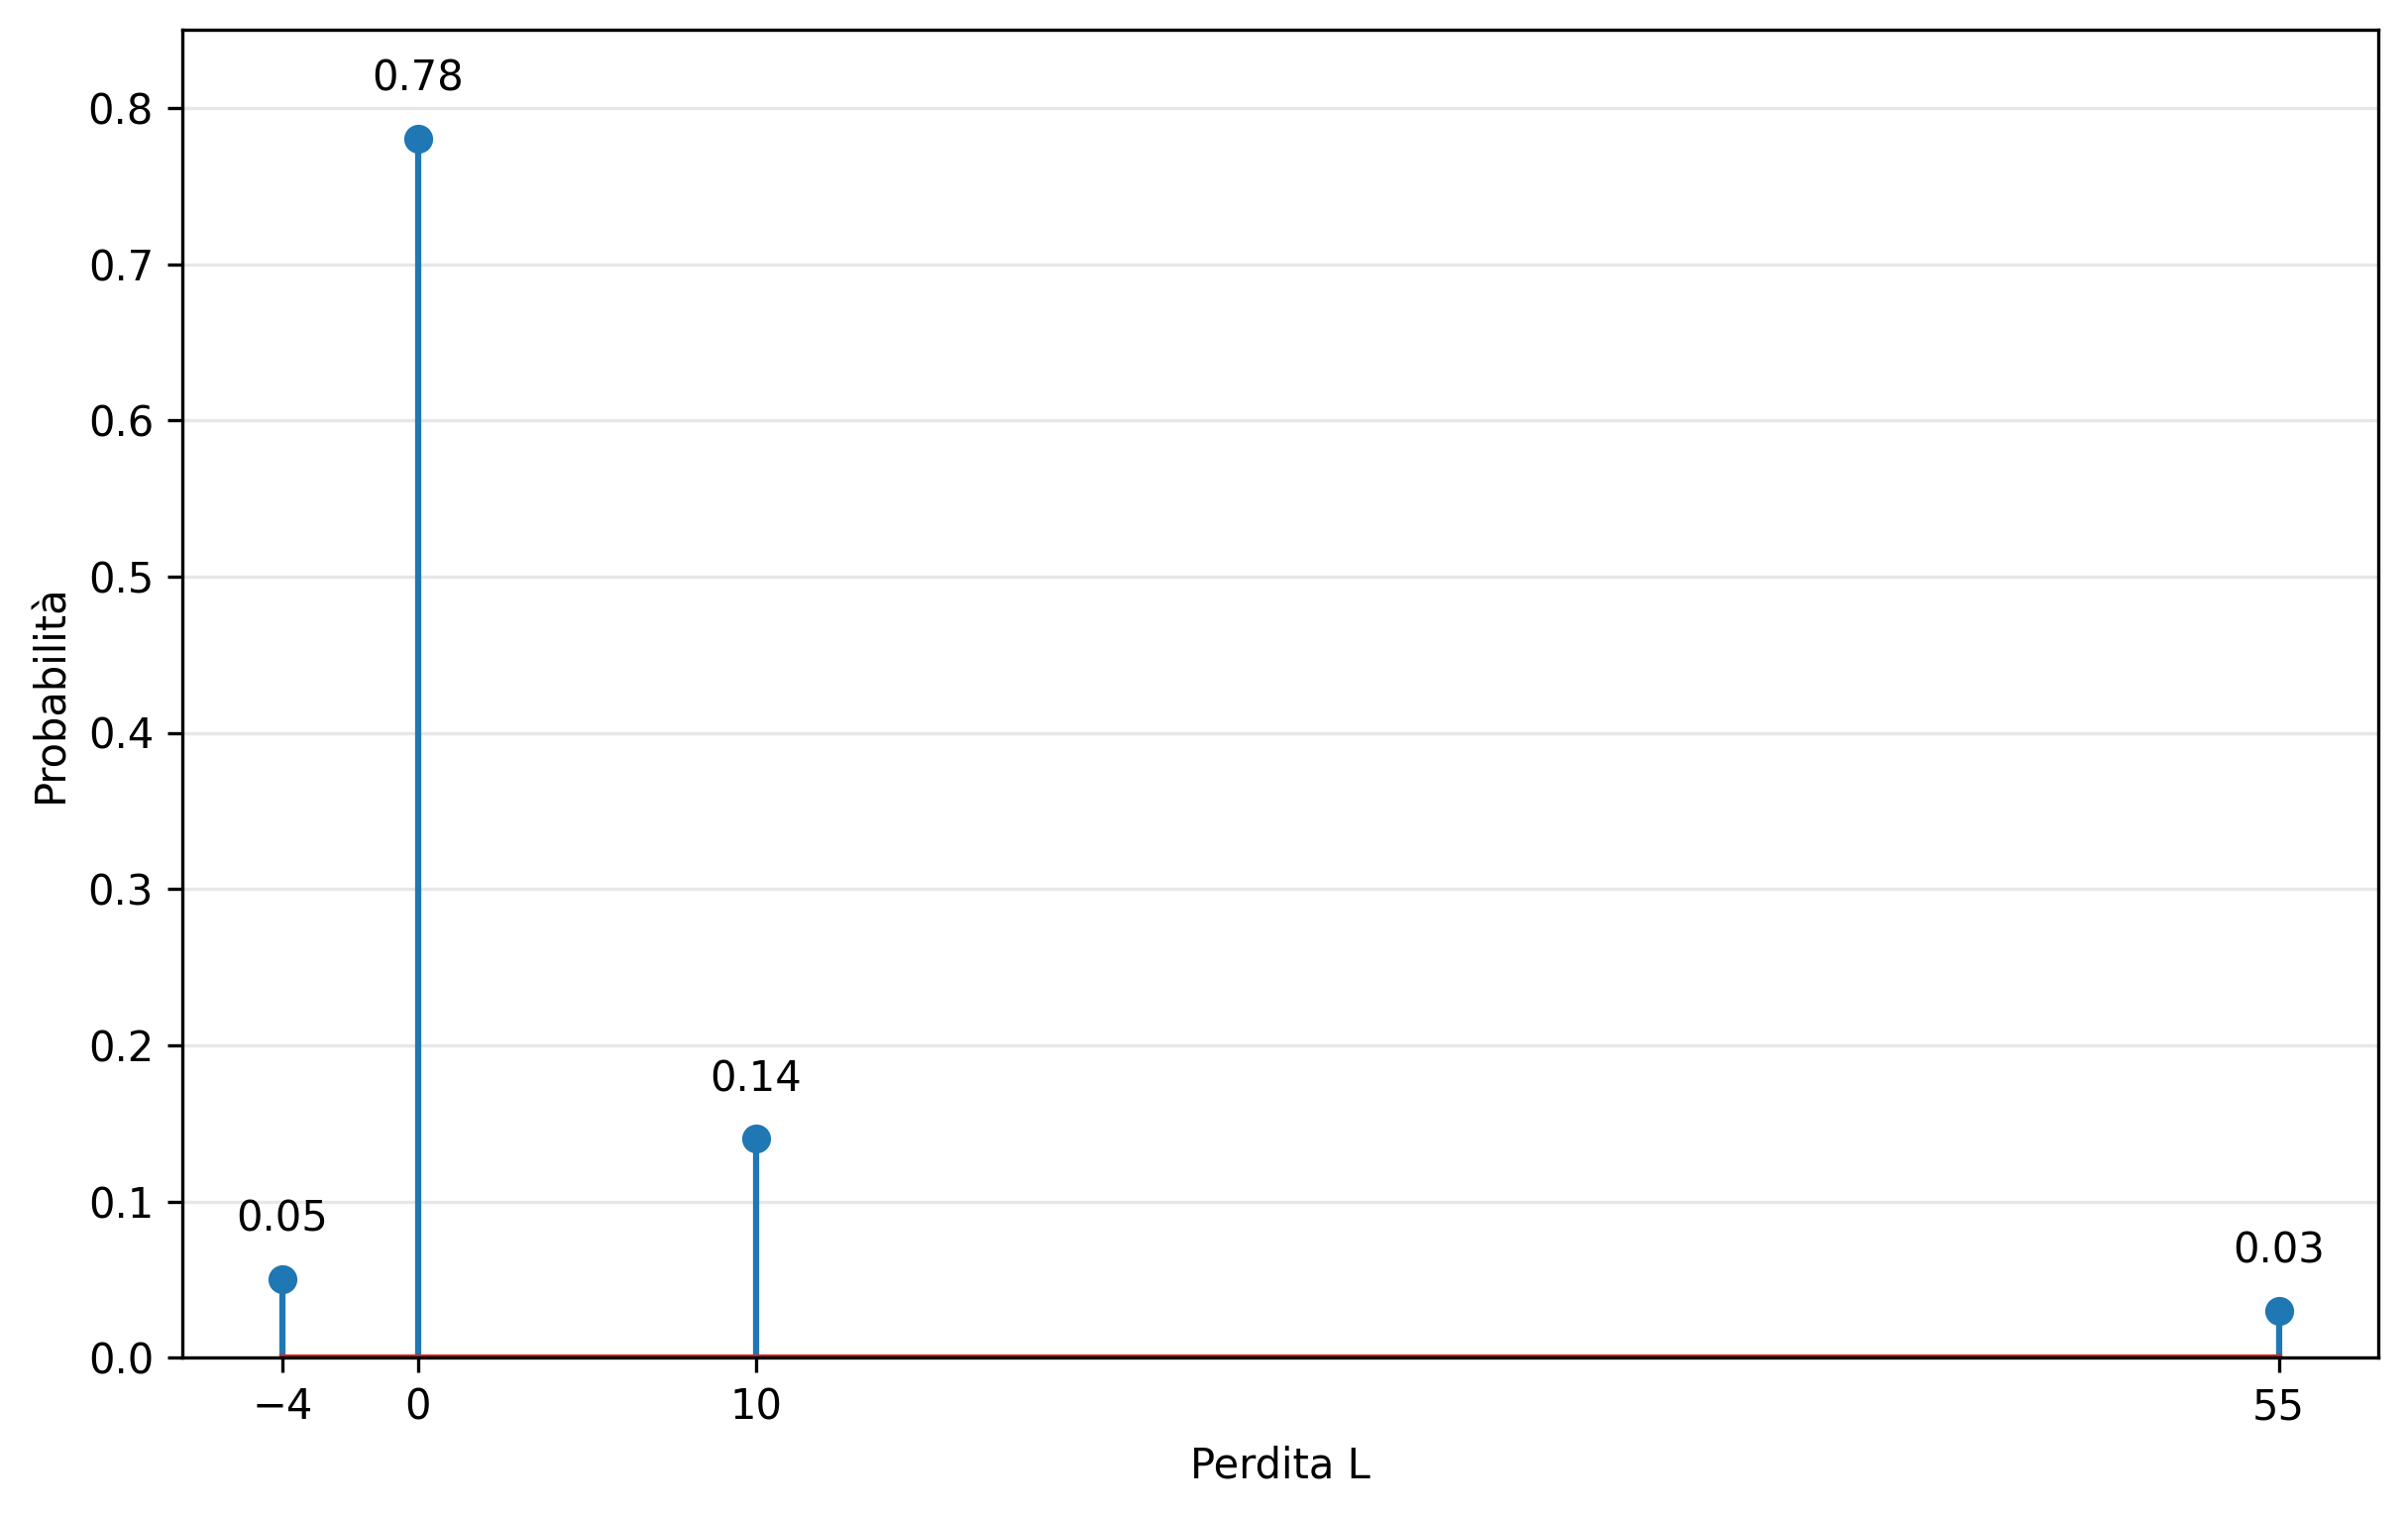
\includegraphics[width=0.78\textwidth]
{../graphics/Cap09_distribuzione_perdita_esercizio.png}
\caption{Funzione di massa della perdita a un anno associata alla
migrazione del rating. La maggior parte della probabilit\`{a} \`{e}
concentrata sulla perdita nulla, mentre il default genera una perdita
elevata ma poco probabile.}
\label{fig:cap09-distribuzione-perdita-esercizio}
\end{figure}

\item La funzione di ripartizione \`{e}

\[
F_{L_1}(\lambda)
=
\Prob(L_1\leq\lambda\mid X_0=2).
\]

Ordinando i possibili valori della perdita,

\[
-4<0<10<55,
\]

si ottiene:

\[
F_{L_1}(\lambda)
=
\begin{cases}
0
&
\text{se }\lambda<-4,
\\
0.05
&
\text{se }-4\leq\lambda<0,
\\
0.83
&
\text{se }0\leq\lambda<10,
\\
0.97
&
\text{se }10\leq\lambda<55,
\\
1
&
\text{se }\lambda\geq55.
\end{cases}
\]

In corrispondenza dei quattro valori della perdita:

\[
\begin{array}{c|cccc}
\lambda
&
-4
&
0
&
10
&
55
\\
\hline
F_{L_1}(\lambda)
&
0.05
&
0.83
&
0.97
&
1
\end{array}
\]

\item La perdita attesa, condizionatamente al rating iniziale, \`{e}

\[
\E^{\Prob}[L_1\mid X_0=2]
=
\sum_{j\in\mathcal{I}}
\ell(j,1)
\Prob(X_1=j\mid X_0=2).
\]

Sostituendo i valori:

\[
\begin{split}
\mathrm{EL}_2(1)
&=
(-4)(0.05)
+
(0)(0.78)
\\
&\quad
+
(10)(0.14)
+
(55)(0.03)
\\
&=
-0.20+0+1.40+1.65
\\
&=
2.85.
\end{split}
\]

Esplicitando i contributi economici:

\[
\begin{split}
\mathrm{EL}_2(1)
&=
\underbrace{(-4)(0.05)}_{\text{upgrade}}
+
\underbrace{(0)(0.78)}_{\text{permanenza}}
\\
&\quad
+
\underbrace{(10)(0.14)}_{\text{downgrade}}
+
\underbrace{(55)(0.03)}_{\text{default}}.
\end{split}
\]

La perdita attesa a un anno \`{e} quindi pari a

\[
\boxed{\mathrm{EL}_2(1)=2.85}.
\]

\item Il momento secondo \`{e}

\[
\E^{\Prob}[L_1^2\mid X_0=2]
=
\sum_{\lambda}
\lambda^2
\Prob(L_1=\lambda\mid X_0=2).
\]

Pertanto,

\[
\begin{split}
\E^{\Prob}[L_1^2\mid X_0=2]
&=
(-4)^2(0.05)
+
0^2(0.78)
\\
&\quad
+
10^2(0.14)
+
55^2(0.03)
\\
&=
16(0.05)
+
100(0.14)
+
3025(0.03)
\\
&=
0.80+14+90.75
\\
&=
105.55.
\end{split}
\]

\item La varianza si ottiene dalla relazione

\[
\Var(L_1\mid X_0=2)
=
\E^{\Prob}[L_1^2\mid X_0=2]
-
\left(
\E^{\Prob}[L_1\mid X_0=2]
\right)^2.
\]

Quindi,

\[
\begin{split}
\Var(L_1\mid X_0=2)
&=
105.55-(2.85)^2
\\
&=
105.55-8.1225
\\
&=
97.4275.
\end{split}
\]

La deviazione standard \`{e}

\[
\begin{split}
\sigma_{L_1}
&=
\sqrt{\Var(L_1\mid X_0=2)}
\\
&=
\sqrt{97.4275}
\\
&\approx
9.87.
\end{split}
\]

\item La distribuzione \`{e} fortemente asimmetrica. Con probabilit\`{a}

\[
0.05+0.78=0.83
\]

l'emittente migliora il proprio rating oppure rimane nella classe
iniziale, producendo una perdita non positiva. La probabilit\`{a} di
una perdita strettamente positiva \`{e} invece

\[
\Prob(L_1>0\mid X_0=2)
=
0.14+0.03
=
0.17.
\]

Il downgrade produce una perdita moderata pari a $10$, mentre il
default produce una perdita molto pi\`{u} elevata, pari a $55$.

Nonostante la probabilit\`{a} di default sia soltanto del $3\%$, il suo
contributo alla perdita attesa \`{e}

\[
55(0.03)=1.65,
\]

superiore al contributo del downgrade:

\[
10(0.14)=1.40.
\]

Il default domina ancora pi\`{u} nettamente il momento secondo:

\[
55^2(0.03)=90.75,
\]

su un valore complessivo pari a $105.55$. La dispersione della perdita
dipende quindi soprattutto dalla presenza di un evento raro ma di
grande severit\`{a}.

\end{enumerate}

\begin{exercise}[VaR e CVaR di una distribuzione discreta]

\label{ex:cap09-var-cvar-discreti}

Si riprenda la distribuzione della perdita a un anno costruita
nell'Esercizio~\ref{ex:cap09-distribuzione-perdita}:

\[
\begin{array}{c|cccc}
\lambda
&
-4
&
0
&
10
&
55
\\
\hline
\Prob(L_1=\lambda\mid X_0=2)
&
0.05
&
0.78
&
0.14
&
0.03
\end{array}
\]

Si consideri il livello di confidenza

\[
\alpha=0.95.
\]

\begin{enumerate}

\item Determinare il $\VaR_{0.95}(L_1)$.

\item Individuare la coda peggiore di probabilit\`{a} $1-\alpha=0.05$
e stabilire quale parte della massa collocata nel punto quantilico
deve essere inclusa nella coda.

\item Calcolare il $\CVaR_{0.95}(L_1)$ come media delle perdite
appartenenti alla coda peggiore del $5\%$.

\item Verificare il risultato mediante la rappresentazione

\[
\CVaR_{\alpha}(L)
=
\min_{\eta\in\R}
\left\{
\eta
+
\frac{1}{1-\alpha}
\E^{\Prob}
\left[
(L-\eta)^{+}
\right]
\right\}.
\]

\item Calcolare

\[
\E^{\Prob}
\left[
L_1
\mid
L_1\geq\VaR_{0.95}(L_1),\ X_0=2
\right]
\]

e spiegare perch\'{e} tale valore non coincide con il
$\CVaR_{0.95}(L_1)$.

\end{enumerate}

\end{exercise}

\noindent
\textbf{Soluzione.}

\begin{enumerate}

\item La funzione di ripartizione della perdita assume, nei punti del
supporto, i valori

\[
\begin{array}{c|cccc}
\lambda
&
-4
&
0
&
10
&
55
\\
\hline
F_{L_1}(\lambda)
&
0.05
&
0.83
&
0.97
&
1
\end{array}
\]

Per definizione,

\[
\VaR_{0.95}(L_1)
=
\inf
\left\{
\lambda\in\R:
F_{L_1}(\lambda)\geq0.95
\right\}.
\]

Poich\'{e}

\[
F_{L_1}(0)=0.83<0.95
\]

e

\[
F_{L_1}(10)=0.97\geq0.95,
\]

si ottiene

\[
\boxed{
\VaR_{0.95}(L_1)=10
}.
\]

Il VaR indica quindi che il quantile di livello $0.95$ della
distribuzione della perdita \`{e} pari a $10$.

\item La coda peggiore deve avere probabilit\`{a}

\[
1-\alpha=0.05.
\]

Le perdite strettamente superiori al VaR comprendono soltanto il valore

\[
L_1=55,
\]

che ha probabilit\`{a}

\[
\Prob(L_1>10\mid X_0=2)=0.03.
\]

Per completare la coda peggiore del $5\%$ occorre quindi includere
un'ulteriore probabilit\`{a}

\[
0.05-0.03=0.02
\]

proveniente dalla massa collocata nel punto quantilico

\[
L_1=10.
\]

La massa complessiva in tale punto \`{e}

\[
\Prob(L_1=10\mid X_0=2)=0.14.
\]

Nella coda entra pertanto soltanto la quota

\[
\frac{0.02}{0.14}
=
\frac{1}{7}
\]

della massa associata alla perdita $10$. La restante probabilit\`{a}

\[
0.14-0.02=0.12
\]

rimane fuori dalla coda peggiore selezionata.

La composizione della coda \`{e} quindi

\[
\begin{array}{c|cc}
\text{perdita}
&
10
&
55
\\
\hline
\text{massa inclusa nella coda}
&
0.02
&
0.03
\end{array}
\]

e le corrispondenti probabilit\`{a} normalizzate sono

\[
\frac{0.02}{0.05}=0.40,
\qquad
\frac{0.03}{0.05}=0.60.
\]

La Figura~\ref{fig:cap09-cvar-massa-quantile-esercizio} mostra la
selezione della coda peggiore del $5\%$.

\begin{figure}[htbp]
\centering
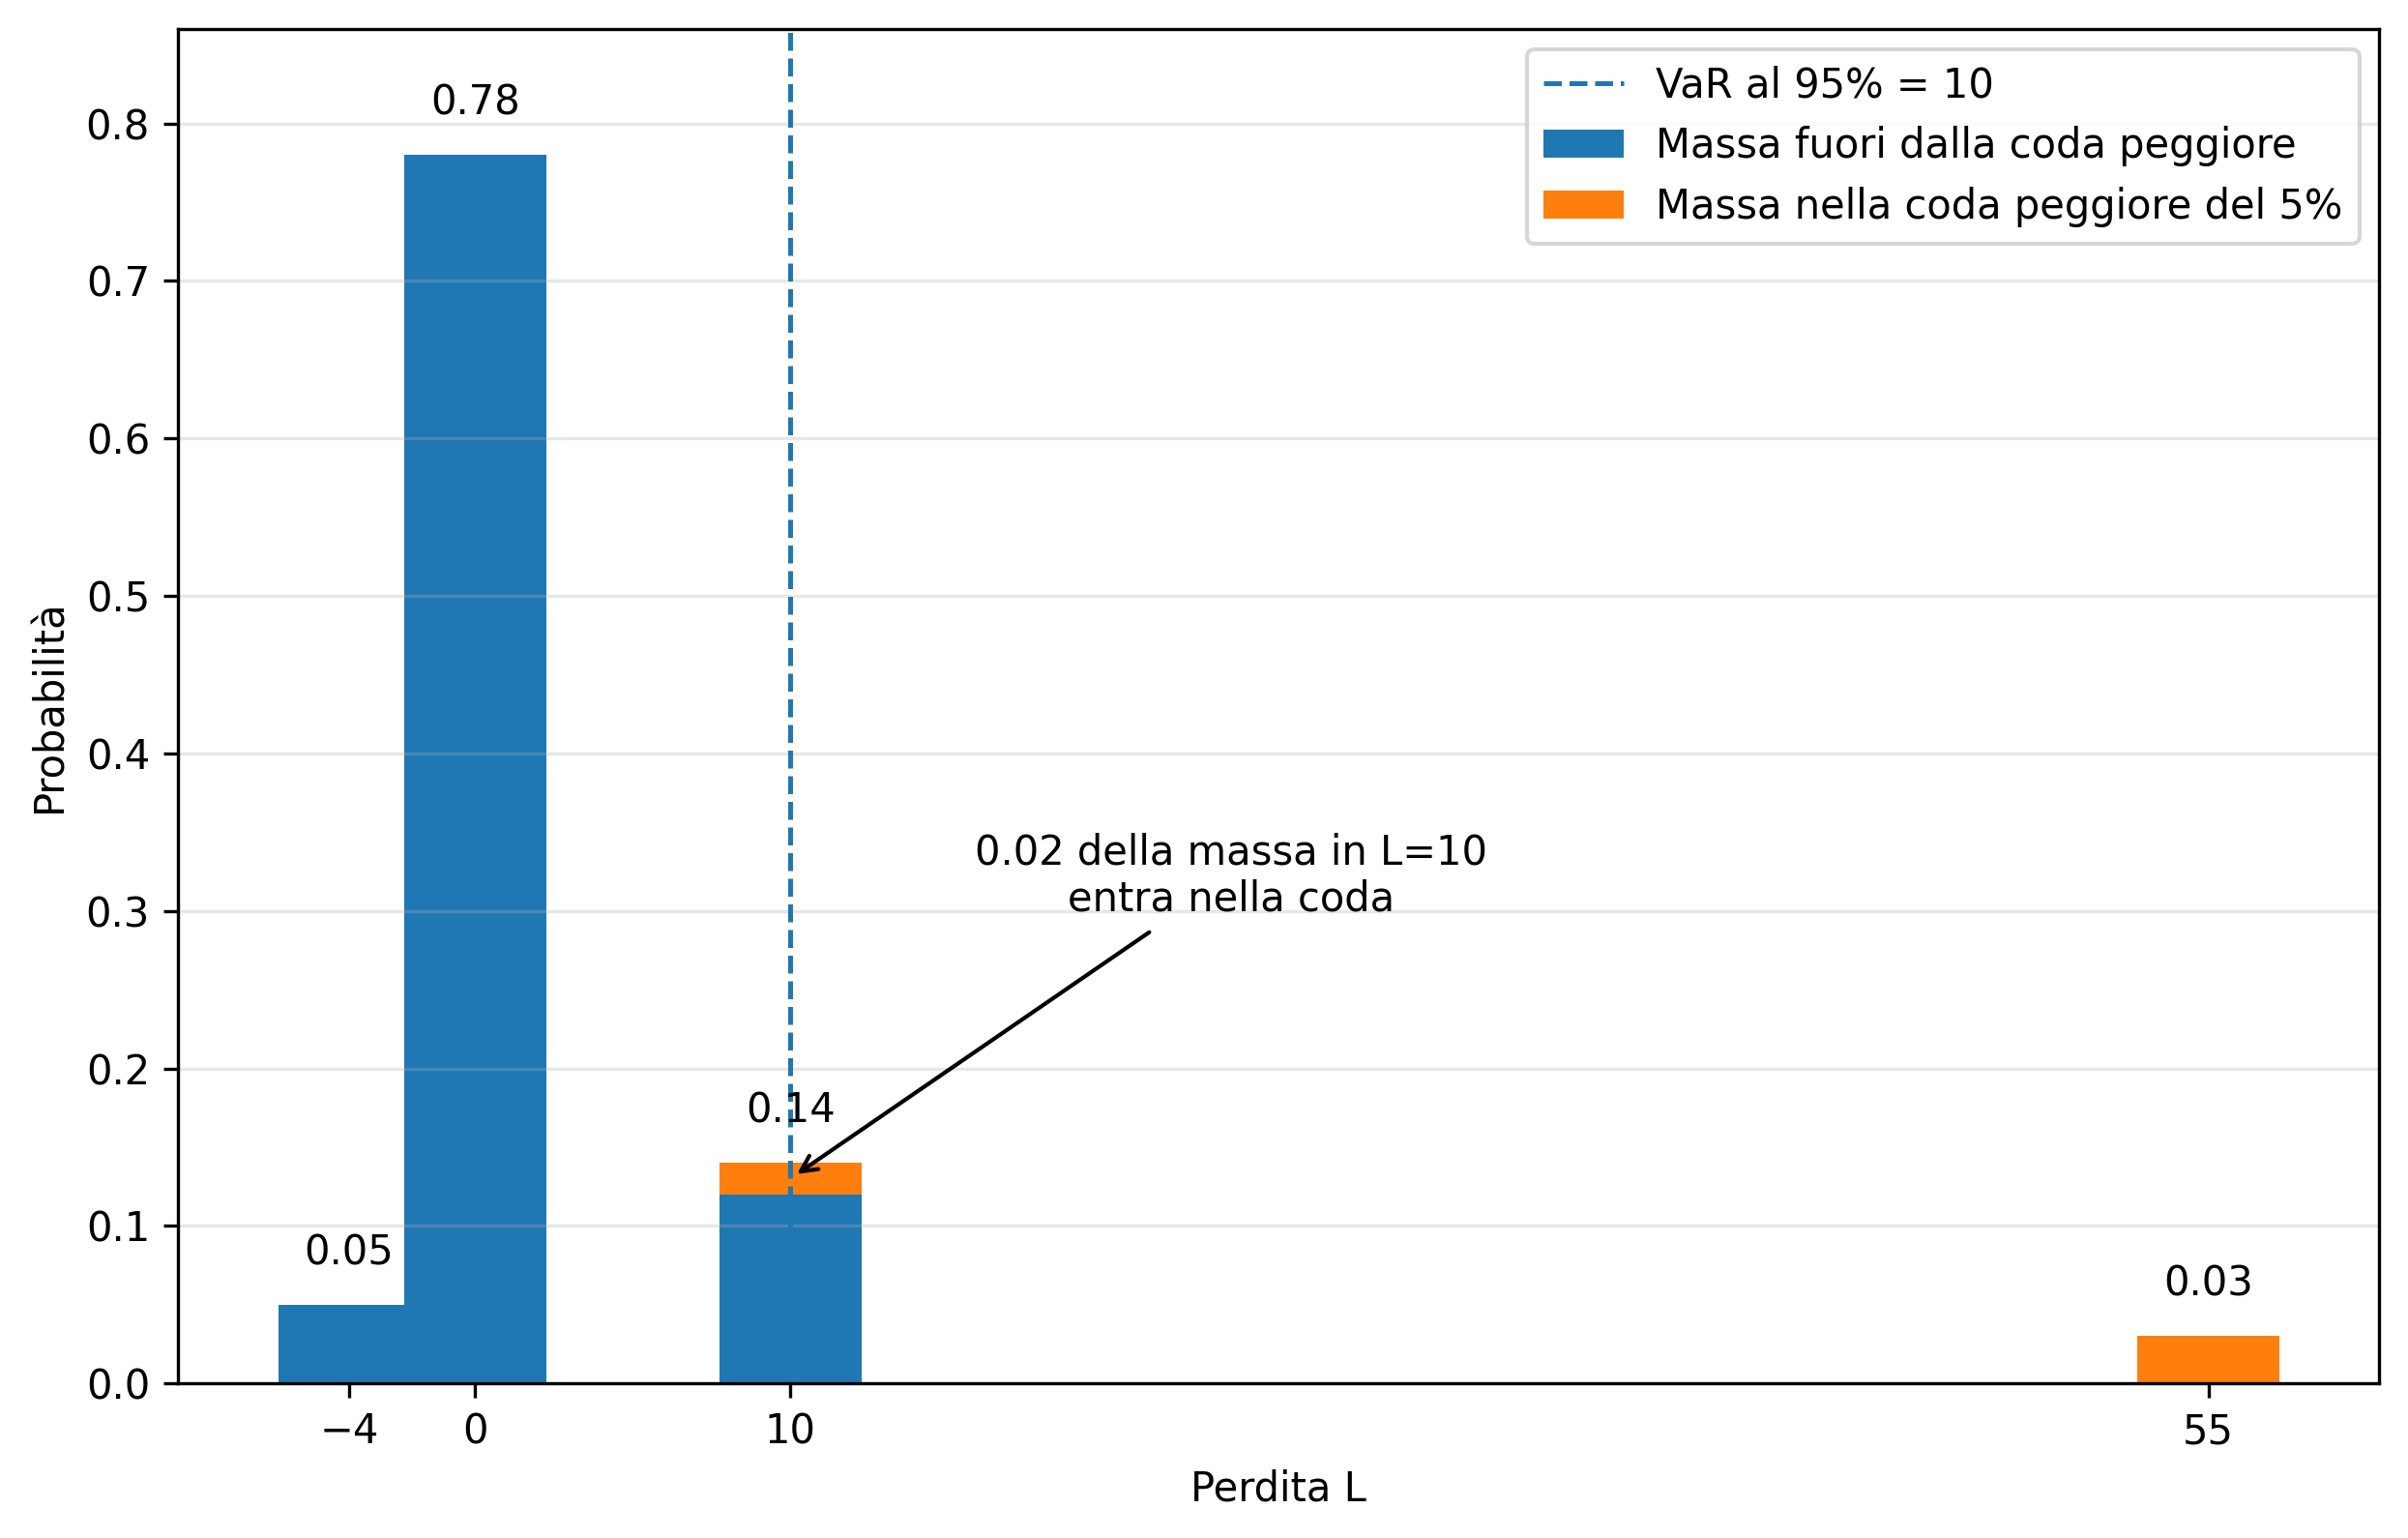
\includegraphics[width=0.82\textwidth]
{../graphics/Cap09_CVaR_massa_quantile_esercizio.png}
\caption{Composizione della coda peggiore del $5\%$. La coda comprende
tutta la massa associata alla perdita $55$ e soltanto una parte della
massa collocata nel punto quantilico $L_1=10$.}
\label{fig:cap09-cvar-massa-quantile-esercizio}
\end{figure}

\item Il CVaR \`{e} la media delle perdite appartenenti alla coda
peggiore, dopo avere normalizzato le masse rispetto alla probabilit\`{a}
complessiva della coda:

\[
\begin{split}
\CVaR_{0.95}(L_1)
&=
10
\frac{0.02}{0.05}
+
55
\frac{0.03}{0.05}
\\
&=
10(0.40)+55(0.60)
\\
&=
4+33
\\
&=
37.
\end{split}
\]

Pertanto,

\[
\boxed{
\CVaR_{0.95}(L_1)=37
}.
\]

Il CVaR \`{e} nettamente superiore al VaR:

\[
\CVaR_{0.95}(L_1)=37
>
10=\VaR_{0.95}(L_1),
\]

poich\'{e} incorpora anche la perdita estrema pari a $55$.

\item Nella rappresentazione basata sulla parte positiva, poniamo

\[
\eta=\VaR_{0.95}(L_1)=10.
\]

Si ha

\[
(L_1-10)^{+}
=
\begin{cases}
0 & \text{se }L_1=-4,\\
0 & \text{se }L_1=0,\\
0 & \text{se }L_1=10,\\
45 & \text{se }L_1=55.
\end{cases}
\]

Pertanto,

\[
\begin{split}
\E^{\Prob}
\left[
(L_1-10)^{+}
\mid X_0=2
\right]
&=
45(0.03)
\\
&=
1.35.
\end{split}
\]

Sostituendo nella formula:

\[
\begin{split}
\CVaR_{0.95}(L_1)
&=
10
+
\frac{1}{1-0.95}(1.35)
\\
&=
10+20(1.35)
\\
&=
10+27
\\
&=
37.
\end{split}
\]

Si ritrova quindi lo stesso risultato:

\[
\boxed{
\CVaR_{0.95}(L_1)=37
}.
\]

La massa parzialmente selezionata al quantile di livello $0.95$ non
compare esplicitamente nel termine

\[
\E^{\Prob}[(L_1-\eta)^{+}],
\]

poich\'{e} per $L_1=\eta=10$ la parte positiva \`{e} nulla. Il suo
effetto \`{e} incorporato nel termine iniziale $\eta$ della
rappresentazione.

\item L'evento

\[
\left\{
L_1\geq\VaR_{0.95}(L_1)
\right\}
\]

comprende tutta la massa associata alle perdite $10$ e $55$. La sua
probabilit\`{a} \`{e}

\[
\Prob(L_1\geq10\mid X_0=2)
=
0.14+0.03
=
0.17.
\]

Il corrispondente valore atteso condizionato \`{e}

\[
\begin{split}
\E^{\Prob}
\left[
L_1
\mid
L_1\geq10,\ X_0=2
\right]
&=
\frac{
10(0.14)+55(0.03)
}{
0.17
}
\\
&=
\frac{1.40+1.65}{0.17}
\\
&=
\frac{3.05}{0.17}
\\
&\approx
17.94.
\end{split}
\]

Si ottiene quindi

\[
\E^{\Prob}
\left[
L_1
\mid
L_1\geq\VaR_{0.95}(L_1),\ X_0=2
\right]
\approx
17.94,
\]

mentre

\[
\CVaR_{0.95}(L_1)=37.
\]

Le due quantit\`{a} non coincidono perch\'{e} l'evento

\[
\{L_1\geq10\}
\]

ha probabilit\`{a} $0.17$, mentre la coda richiesta per il calcolo del
CVaR deve avere probabilit\`{a} esattamente pari a $0.05$.

Il valore atteso condizionato include tutta la massa $0.14$ collocata
nel punto quantilico. Il CVaR include invece soltanto la quota $0.02$
necessaria a completare la coda peggiore del $5\%$.

In presenza di distribuzioni discrete, pertanto,

\[
\CVaR_{\alpha}(L)
\neq
\E^{\Prob}
\left[
L
\mid
L\geq\VaR_{\alpha}(L)
\right]
\]

in generale.

\end{enumerate}

\begin{exercise}[Sensibilit\`{a} dello spread equo di un CDS]

\label{ex:cap09-sensibilita-spread-cds}

Si consideri un CDS con nozionale

\[
N=100
\]

e scadenza $H=3$. I fattori di sconto sono

\[
d_1=0.98,
\qquad
d_2=0.95,
\qquad
d_3=0.92.
\]

Nel primo scenario, le probabilit\`{a} marginali risk-neutral di
default sono

\[
\Prob^{\Q}(\tau_D=1)=0.03,
\qquad
\Prob^{\Q}(\tau_D=2)=0.04,
\qquad
\Prob^{\Q}(\tau_D=3)=0.05.
\]

Le probabilit\`{a} di sopravvivenza sono pertanto

\[
\Prob^{\Q}(\tau_D>1)=0.97,
\qquad
\Prob^{\Q}(\tau_D>2)=0.93,
\qquad
\Prob^{\Q}(\tau_D>3)=0.88.
\]

Si assume che il premio alla data $h$ venga pagato soltanto se
$\tau_D>h$.

\begin{enumerate}

\item Con recovery rate $R=0.40$, calcolare il valore attuale della
gamba di protezione e il coefficiente della gamba dei premi.

\item Determinare lo spread equo $s^*$.

\item Ripetere il calcolo per $R=0.30$ e $R=0.50$, mantenendo
invariate le probabilit\`{a} risk-neutral.

\item Considerare un secondo scenario con probabilit\`{a} marginali
risk-neutral

\[
0.04,
\qquad
0.05,
\qquad
0.07.
\]

Calcolare il nuovo spread equo per $R=0.40$.

\item Interpretare separatamente l'effetto del recovery rate e quello
delle probabilit\`{a} risk-neutral.
\end{enumerate}
\end{exercise}

\noindent
\textbf{Soluzione.}

\begin{enumerate}

\item Introduciamo il fattore attualizzato associato alla gamba di
protezione:

\[
A_{\mathrm{prot}}
=
\sum_{h=1}^{3}
d_h
\Prob^{\Q}(\tau_D=h).
\]

Sostituendo i dati:

\[
\begin{split}
A_{\mathrm{prot}}
&=
(0.98)(0.03)
+
(0.95)(0.04)
+
(0.92)(0.05)
\\
&=
0.0294+0.0380+0.0460
\\
&=
0.1134.
\end{split}
\]

Il valore attuale della gamba di protezione, per $R=0.40$, \`{e}

\[
\begin{split}
\mathrm{PV}_{\mathrm{prot}}
&=
N(1-R)A_{\mathrm{prot}}
\\
&=
100(0.60)(0.1134)
\\
&=
6.804.
\end{split}
\]

Per la gamba dei premi definiamo

\[
A_{\mathrm{prem}}
=
\sum_{h=1}^{3}
d_h
\Prob^{\Q}(\tau_D>h).
\]

Si ottiene:

\[
\begin{split}
A_{\mathrm{prem}}
&=
(0.98)(0.97)
+
(0.95)(0.93)
+
(0.92)(0.88)
\\
&=
0.9506+0.8835+0.8096
\\
&=
2.6437.
\end{split}
\]

Pertanto,

\[
\mathrm{PV}_{\mathrm{prem}}(s)
=
sNA_{\mathrm{prem}}
=
264.37s.
\]

\item Lo spread equo $s^{*}$ rende uguali i valori attuali delle due
gambe:

\[
\mathrm{PV}_{\mathrm{prot}}
=
\mathrm{PV}_{\mathrm{prem}}(s^{*}).
\]

Quindi,

\[
6.804
=
264.37s^{*},
\]

da cui

\[
s^{*}
=
\frac{6.804}{264.37}
\approx
0.02574.
\]

Lo spread equo annuale \`{e} quindi circa

\[
\boxed{
s^{*}=2.574\%
}
\]

ossia

\[
\boxed{
s^{*}\approx257.4\text{ punti base}.
}
\]

Il nozionale compare in entrambe le gambe e si semplifica nella
determinazione dello spread:

\[
s^{*}
=
(1-R)
\frac{
A_{\mathrm{prot}}
}{
A_{\mathrm{prem}}
}.
\]

\begin{figure}[htbp]
\centering
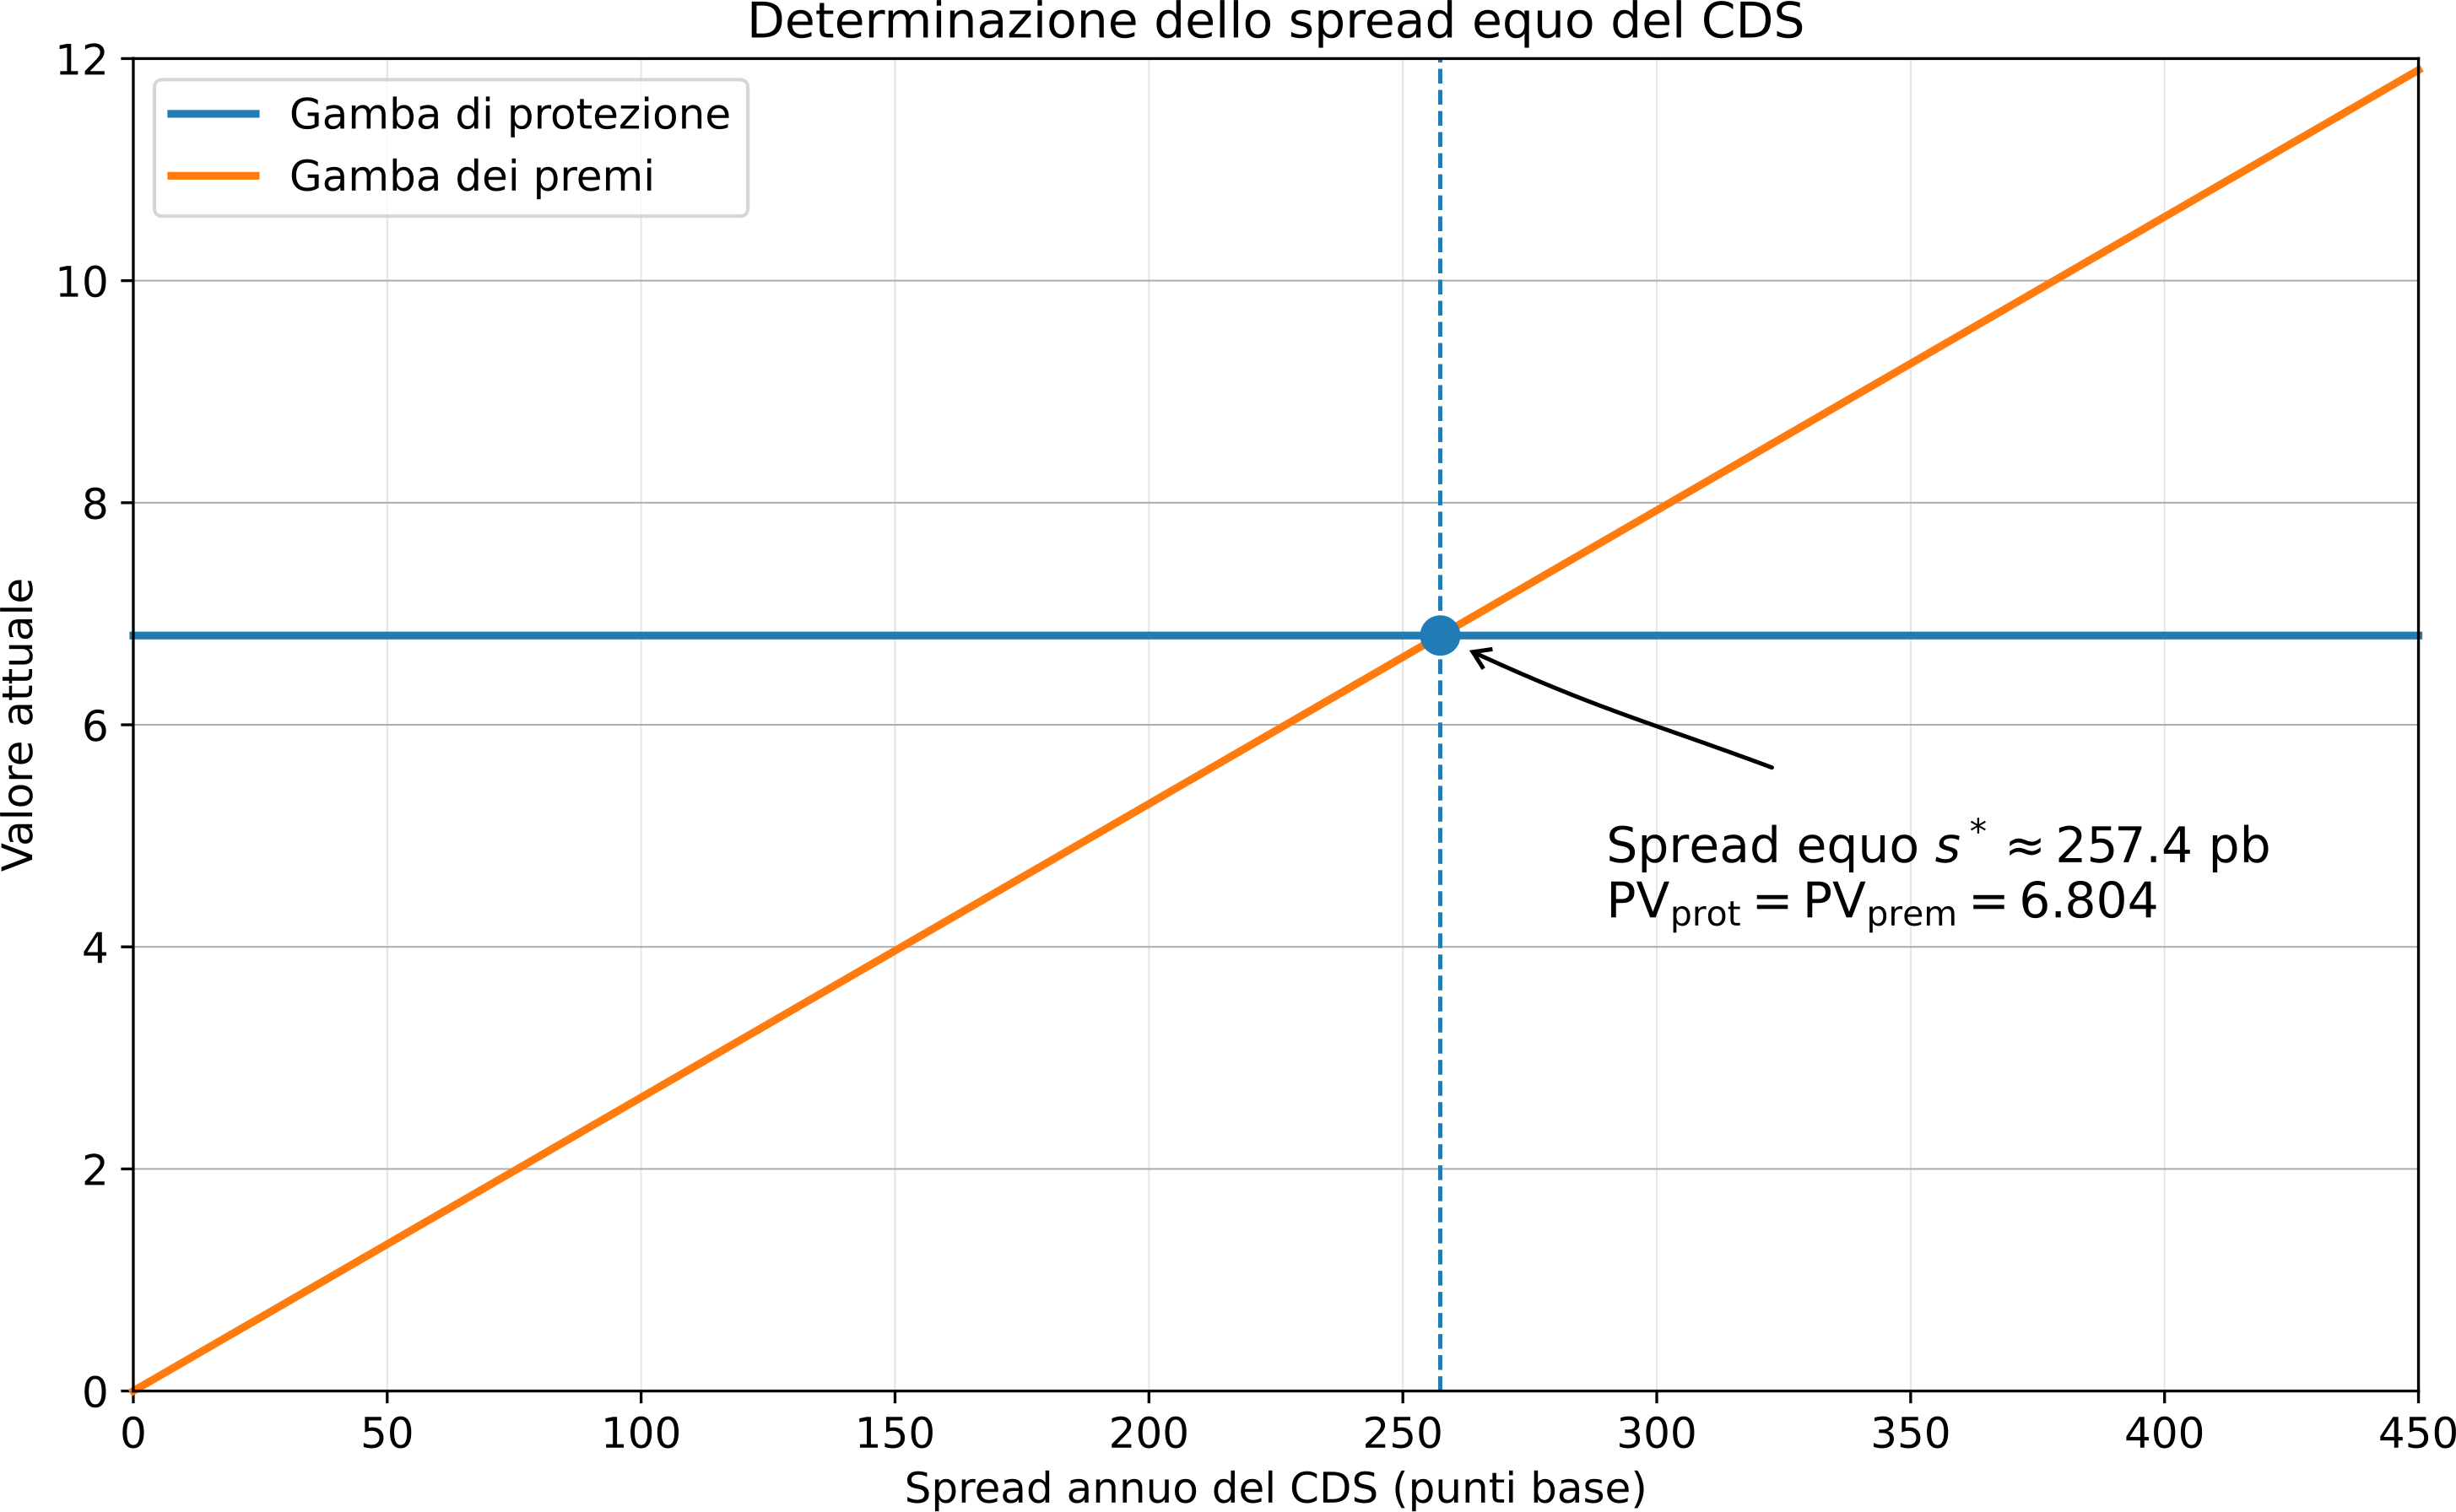
\includegraphics[width=0.90\textwidth]
{../graphics/Cap09_CDS_equilibrio_gambe.png}
\caption{Determinazione dello spread equo del CDS. Il valore attuale
della gamba di protezione non dipende dallo spread contrattuale,
mentre il valore attuale della gamba dei premi cresce linearmente con
esso. Il punto di intersezione identifica lo spread equo
$s^{*}\approx257.4$ punti base, per il quale le due gambe hanno valore
attuale pari a $6.804$.}
\label{fig:cap09-cds-equilibrio-gambe}
\end{figure}

\item Mantenendo invariate le probabilit\`{a} risk-neutral e i fattori
di sconto, la sensibilit\`{a} rispetto al recovery rate \`{e}

\[
s^{*}(R)
=
(1-R)
\frac{0.1134}{2.6437}.
\]

Per $R=0.30$:

\[
\begin{split}
s^{*}(0.30)
&=
0.70
\frac{0.1134}{2.6437}
\\
&\approx
0.03003,
\end{split}
\]

ossia circa

\[
\boxed{
300.3\text{ punti base}.
}
\]

Per $R=0.50$:

\[
\begin{split}
s^{*}(0.50)
&=
0.50
\frac{0.1134}{2.6437}
\\
&\approx
0.02145,
\end{split}
\]

ossia circa

\[
\boxed{
214.5\text{ punti base}.
}
\]

A parit\`{a} delle altre condizioni, un recovery rate pi\`{u} elevato
riduce il pagamento atteso della protezione e quindi riduce lo spread
equo.

\item Nel secondo scenario, le probabilit\`{a} marginali risk-neutral
di default sono

\[
0.04,
\qquad
0.05,
\qquad
0.07.
\]

Le corrispondenti probabilit\`{a} di sopravvivenza sono:

\[
\Prob^{\Q}(\tau_D>1)=0.96,
\]

\[
\Prob^{\Q}(\tau_D>2)
=
1-0.04-0.05
=
0.91,
\]

e

\[
\Prob^{\Q}(\tau_D>3)
=
1-0.04-0.05-0.07
=
0.84.
\]

Il nuovo fattore della gamba di protezione \`{e}

\[
\begin{split}
A_{\mathrm{prot}}^{(2)}
&=
(0.98)(0.04)
+
(0.95)(0.05)
+
(0.92)(0.07)
\\
&=
0.0392+0.0475+0.0644
\\
&=
0.1511.
\end{split}
\]

Il fattore della gamba dei premi \`{e}

\[
\begin{split}
A_{\mathrm{prem}}^{(2)}
&=
(0.98)(0.96)
+
(0.95)(0.91)
+
(0.92)(0.84)
\\
&=
0.9408+0.8645+0.7728
\\
&=
2.5781.
\end{split}
\]

Con $R=0.40$:

\[
\begin{split}
s^{*}_{2}
&=
0.60
\frac{0.1511}{2.5781}
\\
&\approx
0.03517.
\end{split}
\]

Il nuovo spread equo \`{e} quindi

\[
\boxed{
s^{*}_{2}\approx351.7\text{ punti base}.
}
\]

\item Il recovery rate incide sulla severit\`{a} del pagamento di
protezione:

\[
N(1-R).
\]

Mantenendo fisse le probabilit\`{a} risk-neutral, una riduzione di $R$
aumenta quindi lo spread equo.

Un aumento delle probabilit\`{a} risk-neutral di default produce invece
due effetti:

\begin{itemize}

\item aumenta il valore attuale della gamba di protezione;

\item riduce le probabilit\`{a} di sopravvivenza e quindi il valore della
gamba dei premi per ogni unit\`{a} di spread.

\end{itemize}

Entrambi gli effetti determinano un aumento dello spread equo. I
confronti precedenti sono esercizi di sensibilit\`{a} parziale: ogni
parametro viene modificato mantenendo invariati gli altri dati del
modello.

\end{enumerate}

\section{Esercizi proposti}

\label{sec:cap09-esercizi-proposti}

Gli esercizi seguenti riprendono le principali componenti della catena
di misurazione sviluppata nel capitolo. Le applicazioni procedono dal
confronto tra differenti rappresentazioni della perdita creditizia
alla misurazione del rischio di portafoglio e agli scenari di stress.

\begin{exercise}[Modello default-only e modello migration-based]

\label{ex:cap09-default-only-migration-based}

Si considerino due emittenti, $A$ e $B$, inizialmente appartenenti alla
classe di rating $2$. Dopo un anno, le rispettive distribuzioni dei
rating sono:

\[
\begin{array}{c|cccc}
&
1
&
2
&
3
&
D
\\
\hline
A
&
0.08
&
0.75
&
0.14
&
0.03
\\
B
&
0.02
&
0.70
&
0.25
&
0.03
\end{array}
\]

I valori della perdita associati ai quattro stati sono:

\[
\begin{array}{c|cccc}
j
&
1
&
2
&
3
&
D
\\
\hline
\ell(j,1)
&
-3
&
0
&
8
&
60
\end{array}
\]

Nel modello \emph{default-only} si considera soltanto la perdita da
default:

\[
L^{\mathrm{DO}}
=
60\cdot\1_{\{X_1=D\}}.
\]

Nel modello \emph{migration-based} si considera invece

\[
L^{\mathrm{MB}}
=
\ell(X_1,1).
\]

\begin{enumerate}

\item Calcolare, per ciascun emittente, la perdita attesa e la varianza
nel modello \emph{default-only}.

\item Calcolare, per ciascun emittente, la perdita attesa e la varianza
nel modello \emph{migration-based}.

\item Confrontare i risultati ottenuti per gli emittenti $A$ e $B$.

\item Spiegare perch\'{e} la stessa probabilit\`{a} di default non
determina la stessa distribuzione della perdita.

\end{enumerate}

\textit{Risultati:} nel modello \emph{default-only}, per entrambi gli
emittenti,

\[
\mathrm{EL}^{\mathrm{DO}}=1.80,
\qquad
\Var(L^{\mathrm{DO}})=104.76.
\]

Nel modello \emph{migration-based},

\[
\mathrm{EL}^{\mathrm{MB}}_A=2.68,
\qquad
\Var(L_A^{\mathrm{MB}})=110.4976,
\]

mentre

\[
\mathrm{EL}^{\mathrm{MB}}_B=3.74,
\qquad
\Var(L_B^{\mathrm{MB}})=110.1924.
\]

\end{exercise}

\begin{exercise}[Stesso VaR e diverso CVaR]

\label{ex:cap09-stesso-var-diverso-cvar}

Si considerino le due distribuzioni discrete di perdita:

\[
\begin{array}{c|cccc}
\lambda
&
0
&
10
&
20
&
100
\\
\hline
\Prob(L_A=\lambda)
&
0.90
&
0.05
&
0.04
&
0.01
\\
\Prob(L_B=\lambda)
&
0.90
&
0.05
&
0.01
&
0.04
\end{array}
\]

\begin{enumerate}

\item Costruire le funzioni di ripartizione di $L_A$ e $L_B$.

\item Calcolare il VaR al livello di confidenza del $95\%$ per entrambe
le distribuzioni.

\item Calcolare il CVaR al livello di confidenza del $95\%$.

\item Confrontare le due misure e spiegare quale caratteristica della
distribuzione non viene rilevata dal VaR.

\end{enumerate}

\textit{Risultati:}

\[
\VaR_{0.95}(L_A)
=
\VaR_{0.95}(L_B)
=
10,
\]

mentre

\[
\CVaR_{0.95}(L_A)=36,
\qquad
\CVaR_{0.95}(L_B)=84.
\]

Le due distribuzioni hanno lo stesso quantile di livello $0.95$, ma
assegnano probabilit\`{a} molto differenti alla perdita estrema pari
a $100$.

\end{exercise}

\begin{exercise}[Orizzonte temporale e scenario di stress]

\label{ex:cap09-orizzonte-stress}

Si consideri una catena di rating con stati

\[
\mathcal{I}
=
\{
1=\text{qualit\`{a} elevata},
\,
2=\text{qualit\`{a} intermedia},
\,
D=\text{default}
\}.
\]

Nello scenario ordinario, la matrice annuale di transizione \`{e}

\[
P_{\mathrm{ord}}
=
\begin{pmatrix}
0.90&0.08&0.02\\
0.10&0.80&0.10\\
0&0&1
\end{pmatrix}.
\]

In uno scenario di stress viene invece utilizzata la matrice

\[
P_{\mathrm{stress}}
=
\begin{pmatrix}
0.82&0.12&0.06\\
0.05&0.70&0.25\\
0&0&1
\end{pmatrix}.
\]

L'emittente si trova inizialmente nello stato $X_0=2$.

\begin{enumerate}

\item Calcolare $P_{\mathrm{ord}}^2$, $P_{\mathrm{ord}}^3$,
$P_{\mathrm{stress}}^2$ e $P_{\mathrm{stress}}^3$.

\item Determinare le probabilit\`{a} cumulative di default a uno, due
e tre anni nei due scenari.

\item Calcolare le corrispondenti probabilit\`{a} marginali di default
e le probabilit\`{a} di sopravvivenza.

\item Confrontare l'effetto congiunto dell'allungamento dell'orizzonte
e della sostituzione della matrice ordinaria con quella di stress.

\end{enumerate}

\textit{Risultati:} nello scenario ordinario,

\[
\begin{array}{c|ccc}
h
&
1
&
2
&
3
\\
\hline
\mathrm{PD}^{\mathrm{cum}}_2(h)
&
0.1000
&
0.1820
&
0.2502
\\
\mathrm{PD}^{\mathrm{marg}}_2(h)
&
0.1000
&
0.0820
&
0.0682
\\
S_2(h)
&
0.9000
&
0.8180
&
0.7498
\end{array}
\]

Nello scenario di stress,

\[
\begin{array}{c|ccc}
h
&
1
&
2
&
3
\\
\hline
\mathrm{PD}^{\mathrm{cum}}_2(h)
&
0.2500
&
0.4280
&
0.5566
\\
\mathrm{PD}^{\mathrm{marg}}_2(h)
&
0.2500
&
0.1780
&
0.1286
\\
S_2(h)
&
0.7500
&
0.5720
&
0.4434
\end{array}
\]

\end{exercise}

\begin{exercise}[Posizione coperta e posizione non coperta]

\label{ex:cap09-copertura-cds}

La perdita di una posizione creditizia non coperta presenta la
distribuzione:

\[
\begin{array}{c|cccc}
\text{stato}
&
1
&
2
&
3
&
D
\\
\hline
\Prob(X_1=j)
&
0.10
&
0.72
&
0.14
&
0.04
\\
L^{\mathrm{unhedged}}
&
-2
&
0
&
12
&
50
\end{array}
\]

Un CDS paga $50$ in caso di default e nulla negli altri stati. Il
valore attuale equivalente dei premi \`{e} pari a $2.5$ ed \`{e}
trattato, in questo modello semplificato, come un costo certo.

La perdita coperta \`{e} quindi

\[
L^{\mathrm{hedged}}
=
L^{\mathrm{unhedged}}
-
50\cdot\1_{\{X_1=D\}}
+
2.5.
\]

\begin{enumerate}

\item Costruire la distribuzione della perdita coperta.

\item Calcolare la perdita attesa, il VaR al $95\%$ e il CVaR al
$95\%$ della posizione non coperta.

\item Calcolare le stesse misure per la posizione coperta.

\item Spiegare perch\'{e} la copertura pu\`{o} ridurre il CVaR senza
ridurre necessariamente la perdita attesa o il VaR.

\end{enumerate}

\textit{Risultati:} per la posizione non coperta,

\[
\mathrm{EL}^{\mathrm{unhedged}}=3.48,
\qquad
\VaR_{0.95}(L^{\mathrm{unhedged}})=12,
\]

\[
\CVaR_{0.95}(L^{\mathrm{unhedged}})=42.4.
\]

La distribuzione della posizione coperta \`{e}

\[
\begin{array}{c|ccc}
\lambda
&
0.5
&
2.5
&
14.5
\\
\hline
\Prob(L^{\mathrm{hedged}}=\lambda)
&
0.10
&
0.76
&
0.14
\end{array}
\]

e

\[
\mathrm{EL}^{\mathrm{hedged}}=3.98,
\qquad
\VaR_{0.95}(L^{\mathrm{hedged}})=14.5,
\]

\[
\CVaR_{0.95}(L^{\mathrm{hedged}})=14.5.
\]

\end{exercise}

\begin{exercise}[Dipendenza tra due esposizioni]

\label{ex:cap09-portafoglio-dipendenza}

Un portafoglio contiene due esposizioni. In caso di default del primo
emittente si verifica una perdita pari a $40$; in caso di default del
secondo emittente si verifica una perdita pari a $60$.

Le due probabilit\`{a} individuali di default sono

\[
\Prob(X_{1,h}=D)
=
\Prob(X_{2,h}=D)
=
0.05.
\]

Si confrontino due modelli:

\begin{itemize}

\item default indipendenti;

\item dipendenza positiva perfetta, per la quale i due emittenti
entrano sempre in default congiuntamente.

\end{itemize}

La perdita di portafoglio \`{e}

\[
L_h^{\mathrm{port}}
=
40\1_{\{X_{1,h}=D\}}
+
60\1_{\{X_{2,h}=D\}}.
\]

\begin{enumerate}

\item Costruire la distribuzione congiunta dei due indicatori di
default nei due modelli.

\item Determinare la distribuzione della perdita aggregata.

\item Calcolare la perdita attesa nei due casi.

\item Calcolare il VaR e il CVaR al livello di confidenza del $95\%$.

\item Spiegare perch\'{e} la perdita attesa rimane invariata, mentre
le misure di coda cambiano sensibilmente.

\end{enumerate}

\textit{Risultati:} sotto indipendenza,

\[
\begin{array}{c|cccc}
\lambda
&
0
&
40
&
60
&
100
\\
\hline
\Prob(L_h^{\mathrm{port}}=\lambda)
&
0.9025
&
0.0475
&
0.0475
&
0.0025
\end{array}
\]

e

\[
\E^{\Prob}[L_h^{\mathrm{port}}]=5,
\qquad
\VaR_{0.95}(L_h^{\mathrm{port}})=40,
\]

\[
\CVaR_{0.95}(L_h^{\mathrm{port}})=62.
\]

Sotto dipendenza positiva perfetta,

\[
\begin{array}{c|cc}
\lambda
&
0
&
100
\\
\hline
\Prob(L_h^{\mathrm{port}}=\lambda)
&
0.95
&
0.05
\end{array}
\]

e

\[
\E^{\Prob}[L_h^{\mathrm{port}}]=5,
\qquad
\VaR_{0.95}(L_h^{\mathrm{port}})=0,
\]

\[
\CVaR_{0.95}(L_h^{\mathrm{port}})=100.
\]

\end{exercise}

\section{Sintesi e raccordo con la Lezione 10}

\label{sec:cap09-sintesi-raccordo}

Il capitolo ha sviluppato il passaggio dalle probabilit\`{a} di
transizione tra rating alla distribuzione monetaria delle perdite
creditizie. La costruzione richiede di collegare tre componenti:
l'evoluzione probabilistica degli stati, le conseguenze economiche
associate a ciascuno stato futuro e le misure utilizzate per descrivere
la distribuzione della perdita.

La sequenza concettuale complessiva pu\`{o} essere sintetizzata come
segue:

\[
\boxed{
\begin{array}{c}
\text{PD marginali, cumulative e sopravvivenza}
\\[2mm]
\downarrow
\\[2mm]
\text{PD, LGD, EAD e valori associati ai rating}
\\[2mm]
\downarrow
\\[2mm]
\text{distribuzione della perdita}
\\[2mm]
\downarrow
\\[2mm]
\text{\emph{Expected Loss}, \emph{VaR} e \emph{CVaR}}
\\[2mm]
\downarrow
\\[2mm]
P^{\Prob}\ \text{per il rischio}
\qquad
P^{\Q}\ \text{per il pricing}
\\[2mm]
\downarrow
\\[2mm]
\text{CDS e copertura}
\\[2mm]
\downarrow
\\[2mm]
\text{portafoglio, dipendenza e simulazione}
\end{array}
}
\]

Le potenze della matrice di transizione permettono anzitutto di
determinare la struttura temporale del default. La probabilit\`{a}
cumulativa misura il rischio di default entro un dato orizzonte; la
probabilit\`{a} marginale isola il contributo del singolo periodo; la
probabilit\`{a} di sopravvivenza descrive la permanenza negli stati
non-default.

Queste probabilit\`{a} non determinano, da sole, una distribuzione
monetaria. Occorre associare a ciascuno stato futuro una conseguenza
economica. Nel modello default-only la perdita dipende essenzialmente
da \emph{Exposure at Default} (\emph{EAD}) e \emph{Loss Given Default}
(\emph{LGD}); nel modello basato sulle migrazioni del rating assume
rilievo anche la variazione del valore dell'esposizione negli stati
non-default.

La funzione di perdita realizza tale passaggio:

\[
L_h=\ell(X_h,h),
\qquad
\ell(j,h)=V^{\mathrm{ref}}(h)-V_j(h).
\]

Una volta costruita la distribuzione di $L_h$, la
\emph{Expected Loss} (\emph{EL}) ne misura il valore medio, mentre il
\emph{Value at Risk} (\emph{VaR}) e il \emph{Conditional Value at
Risk} (\emph{CVaR}) descrivono la parte superiore della distribuzione.
Il VaR individua un quantile della perdita; il CVaR considera anche la
severit\`{a} degli esiti appartenenti alla coda peggiore. Nel caso di
distribuzioni discrete, il suo calcolo pu\`{o} richiedere l'inclusione
parziale della massa associata al valore del VaR.

La distinzione tra misura fisica e misura risk-neutral separa due
finalit\`{a} differenti. Le probabilit\`{a} sotto $\Prob$ vengono
utilizzate per prevedere le perdite e misurare il rischio. Le
probabilit\`{a} sotto $\Q$ vengono invece utilizzate per valutare i
flussi finanziari coerentemente con i prezzi di mercato.

Nel caso del \emph{Credit Default Swap} (\emph{CDS}), il premio equo
rende uguali il valore attuale della gamba dei premi e quello della
gamba di protezione. La copertura modifica la distribuzione della
perdita, ma non elimina necessariamente tutte le sue componenti. Il
costo dei premi, le perdite da downgrade, il rischio di controparte e
il \emph{basis risk} possono produrre una posizione residua ancora
esposta al rischio creditizio.

Il passaggio dalla singola esposizione al portafoglio introduce infine
la dipendenza tra i debitori. La perdita aggregata

\[
L_h^{\mathrm{port}}
=
\sum_{n=1}^{N}L_{n,h}
\]

dipende non soltanto dalle distribuzioni individuali, ma anche dalla
probabilit\`{a} che downgrade e default si verifichino congiuntamente.
Concentrazione, fattori macroeconomici comuni e rischio sistematico
assumono quindi un ruolo essenziale nella determinazione delle perdite
estreme.

La Lezione~10 svilupper\`{a} operativamente questo ultimo passaggio.
Per portafogli con molte esposizioni, il numero delle possibili
configurazioni dei rating cresce rapidamente e rende poco praticabile
la costruzione analitica della distribuzione congiunta. La simulazione
permette invece di generare un numero elevato di scenari e di
ricostruire empiricamente la distribuzione della perdita aggregata.

In ciascuna replica della simulazione si proceder\`{a} a:

\begin{enumerate}

\item generare gli eventuali fattori economici comuni;

\item simulare le transizioni dei singoli emittenti, condizionatamente
ai rating iniziali e ai fattori comuni;

\item associare a ciascuno stato futuro la corrispondente perdita e
aggregare le perdite individuali;

\item ripetere la procedura per stimare la distribuzione della perdita
di portafoglio, la perdita attesa e le misure di rischio di coda.

\end{enumerate}

Il raccordo tra le due lezioni pu\`{o} quindi essere sintetizzato come
segue:

\[
\boxed{
\begin{array}{c}
\text{Lezione 9}
\\
\text{costruzione teorica della distribuzione della perdita}
\\[2mm]
\downarrow
\\[2mm]
\text{Lezione 10}
\\
\text{simulazione della distribuzione di portafoglio}
\\[2mm]
\downarrow
\\[2mm]
\text{stima empirica di EL, VaR e CVaR}
\end{array}
}
\]

}}%
%BeginExpansion
% !TeX root = ../MQF_Manuale_Master.tex
% Capitoli/MQF_Cap_09_Markov_Misure_Rischio.tex

\chapter{Catene di Markov e misure di rischio}

\label{cap:markov-misure-rischio}

\section{Obiettivi della lezione e problema guida}

\label{sec:cap9-obiettivi}

Nel Capitolo~8 la dinamica di un sistema economico o finanziario \`{e}
stata rappresentata mediante una catena di Markov finita. Assegnata una
matrice di transizione $P$, le sue potenze determinano le
probabilit\`{a} degli stati futuri:

\[
p_{ij}^{(h)}
=
\Prob(X_h=j\mid X_0=i)
=
(P^h)_{ij}.
\]

Se lo stato iniziale non \`{e} noto con certezza ed \`{e} descritto
dalla distribuzione $\pi_0$, la distribuzione degli stati
all'orizzonte $h$ \`{e}

\[
\pi_h=\pi_0P^h.
\]

Nel caso delle migrazioni del rating, questi risultati permettono di
determinare la probabilit\`{a} che un emittente migliori il proprio
merito creditizio, rimanga nella classe corrente, subisca un
deterioramento oppure entri nello stato assorbente di default.

La distribuzione degli stati futuri non coincide tuttavia con una
distribuzione delle perdite. La matrice di transizione descrive
\emph{quali stati possono verificarsi e con quale probabilit\`{a}}, ma
non stabilisce automaticamente quali conseguenze economiche derivino
da ciascuno stato.

Per mettere in evidenza questa distinzione, consideriamo due esposizioni
creditizie $A$ e $B$, aventi lo stesso nozionale, la stessa
scadenza e il medesimo tasso di recupero. Supponiamo inoltre che le due
esposizioni presentino la stessa probabilit\`{a} annuale di default,
pari al $3\%$, ma differenti probabilit\`{a} di migrazione:

\[
\begin{array}{lcccc}
\hline
&
\text{miglioramento}
&
\text{rating invariato}
&
\text{downgrade}
&
\text{default}
\\
\hline
\text{Esposizione }A
&
0.04
&
0.78
&
0.15
&
0.03
\\
\text{Esposizione }B
&
0.08
&
0.87
&
0.02
&
0.03
\\
\hline
\end{array}
\]

Se si osservasse soltanto la probabilit\`{a} di default, le due
esposizioni potrebbero apparire equivalenti. L'esposizione $A$
presenta per\`{o} una probabilit\`{a} di downgrade molto pi\`{u}
elevata. Se il deterioramento del rating determina un aumento del
credit spread e una riduzione del valore di mercato dello strumento,
la distribuzione delle perdite di $A$ pu\`{o} risultare sensibilmente
diversa da quella di $B$, anche se la probabilit\`{a} di default
\`{e} identica.

L'esempio mostra che la probabilit\`{a} di default costituisce una
componente essenziale del rischio di credito, ma non ne fornisce una
misura completa. Per passare dalle probabilit\`{a} alle perdite occorre
specificare almeno:

\begin{itemize}

\item l'esposizione economica soggetta a rischio;

\item la perdita subita in caso di default;

\item il valore recuperabile dopo il default;

\item la variazione di valore prodotta dalle migrazioni verso rating
migliori o peggiori;

\item l'orizzonte temporale sul quale il rischio viene misurato.

\end{itemize}

Il problema guida del capitolo \`{e} pertanto il seguente:

\begin{quote}
\emph{Come possiamo utilizzare le probabilit\`{a} di migrazione e di
default generate da una catena di Markov per costruire una
distribuzione monetaria delle perdite, misurare il rischio della sua
coda e valutare l'effetto di uno strumento di copertura come il credit
default swap?}
\end{quote}

Il percorso concettuale della lezione pu\`{o} essere rappresentato
mediante la sequenza

\[
P^h
\longrightarrow
\text{default e sopravvivenza}
\longrightarrow
L_h
\longrightarrow
\VaR_{\alpha}(L_h)
\longrightarrow
\CVaR_{\alpha}(L_h)
\longrightarrow
\text{CDS}.
\]

La matrice $P^h$ determina le probabilit\`{a} dei rating futuri e,
in particolare, la struttura temporale delle probabilit\`{a} di
default e di sopravvivenza. Associando a ciascuno stato futuro un
valore economico o una perdita si costruisce la variabile casuale
$L_h$. La sua distribuzione permette di calcolare la perdita attesa
e le misure di rischio di coda. Le stesse probabilit\`{a} di default e
sopravvivenza costituiscono inoltre gli elementi probabilistici
necessari per rappresentare i flussi di un credit default swap.

Il CDS introduce una seconda domanda finanziaria. La distribuzione
delle perdite serve a misurare il rischio di una posizione creditizia;
il valore del derivato serve invece a determinare il prezzo di mercato
della protezione. Le due analisi utilizzano lo stesso scheletro
markoviano, ma richiedono una diversa interpretazione delle
probabilit\`{a}: le probabilit\`{a} fisiche sono utilizzate per la
previsione e la misurazione del rischio, mentre le probabilit\`{a}
risk-neutral sono utilizzate per il pricing dei flussi finanziari.

Al termine del capitolo lo studente dovr\`{a} essere in grado di:

\begin{itemize}

\item ricavare dalle potenze della matrice di transizione le
probabilit\`{a} cumulative e marginali di default e le
probabilit\`{a} di sopravvivenza;

\item interpretare e utilizzare i parametri fondamentali del rischio di
credito, quali probability of default, loss given default, exposure at
default e recovery rate;

\item distinguere un modello che considera soltanto il default da un
modello che include anche le perdite prodotte dalle migrazioni del
rating;

\item associare agli stati creditizi futuri valori e perdite monetarie,
costruendo la variabile casuale $L_h$ e la relativa distribuzione;

\item calcolare e interpretare perdita attesa, varianza,
$\VaR_{\alpha}$, $\CVaR_{\alpha}$ e capitale economico;

\item distinguere l'impiego delle probabilit\`{a} fisiche nella
misurazione del rischio dall'impiego delle probabilit\`{a} risk-neutral
nella valutazione finanziaria;

\item rappresentare, in un modello discreto semplificato, la gamba dei
premi e la gamba di protezione di un credit default swap e determinarne
il premio equo;

\item confrontare la distribuzione delle perdite di una posizione
creditizia non coperta con quella della corrispondente posizione
protetta mediante CDS;

\item riconoscere il ruolo della dipendenza, della concentrazione e del
rischio di modello nel passaggio dalla singola esposizione al
portafoglio creditizio.

\end{itemize}

Il capitolo utilizzer\`{a} come riferimento principale una catena di
migrazione del rating con default assorbente. Lo stesso caso verr\`{a}
sviluppato progressivamente, passando dalle probabilit\`{a} degli stati
futuri alle perdite monetarie, dalle perdite alle misure di rischio e,
infine, dalla misurazione del rischio alla valutazione e all'impiego di
uno strumento di copertura.

\section{Dalla matrice di transizione alla struttura temporale del
default}

\label{sec:cap9-struttura-temporale-default}

Nel Capitolo~8 la colonna della matrice $P^{h}$ associata allo stato
di default \`{e} stata interpretata come distribuzione della
probabilit\`{a} assorbita in tale stato all'orizzonte $h$. Per
utilizzare questa informazione nella misurazione delle perdite e nella
valutazione dei contratti creditizi occorre ora distinguere quattro
quantit\`{a}:

\begin{itemize}

\item la probabilit\`{a} che il default si sia verificato entro
l'orizzonte $h$;

\item la probabilit\`{a} che il default si verifichi precisamente nel
periodo $h$;

\item la probabilit\`{a} che l'emittente sopravviva oltre $h$;

\item la probabilit\`{a} di default nel periodo $h$, condizionata alla
sopravvivenza fino al periodo precedente.

\end{itemize}

Queste quantit\`{a} derivano tutte dalla stessa matrice di transizione,
ma rispondono a domande differenti.

\subsection{Tempo di default e stato assorbente}

\label{subsec:cap9-tempo-default}

Consideriamo una catena di Markov omogenea
\[
\{X_h\}_{h=0}^{H}
\]
con spazio degli stati
\[
\mathcal{I}
=
\{1,\ldots,m-1,D\},
\]
dove $D$ rappresenta il default.

Come nel modello di migrazione del rating introdotto nel
Capitolo~8, assumiamo che il default sia uno stato assorbente:

\[
p_{DD}=1.
\]

Una volta entrata nello stato $D$, la catena non pu\`{o} quindi
ritornare negli stati non-default.

\begin{definition}
Per un emittente inizialmente non in default, il \emph{tempo di
default} \`{e} la variabile casuale

\[
\tau_D
=
\inf
\{
h\geq 1:X_h=D
\}.
\]

Se lo stato $D$ non viene mai raggiunto nell'orizzonte considerato,
si adotta la convenzione

\[
\inf\varnothing=+\infty.
\]
\end{definition}

La variabile $\tau_D$ indica il primo periodo nel quale l'emittente
entra nello stato di default. Ad esempio,

\[
\{\tau_D=2\}
\]

rappresenta l'evento in cui l'emittente sopravvive al primo periodo ed
entra in default nel secondo.

La natura assorbente dello stato $D$ implica, per ogni $h\geq 1$,

\[
\{\tau_D\leq h\}
=
\{X_h=D\}.
\]

Infatti, se il default si verifica entro il periodo $h$, la catena
rimane nello stato $D$ fino alla data $h$. Viceversa, se
$X_h=D$, la catena deve essere entrata nello stato di default in uno
dei periodi $1,\ldots,h$.

Questa equivalenza dipende in modo essenziale dall'assorbimento. Se la
catena potesse uscire dallo stato $D$, il fatto che il default si sia
verificato in passato non implicherebbe necessariamente che il sistema
si trovi ancora nello stato $D$ alla data $h$.

\subsection{Probabilit\`{a} cumulativa di default}

\label{subsec:cap9-pd-cumulativa}

\begin{definition}
Per un emittente inizialmente nello stato non-default
$i\in\mathcal{I}\setminus\{D\}$, la \emph{probabilit\`{a} cumulativa
di default} entro l'orizzonte $h$ \`{e}

\[
\mathrm{PD}_{i}^{\mathrm{cum}}(h)
=
\Prob(\tau_D\leq h\mid X_0=i).
\]
\end{definition}

Utilizzando l'equivalenza

\[
\{\tau_D\leq h\}
=
\{X_h=D\},
\]

si ottiene

\[
\begin{split}
\mathrm{PD}_{i}^{\mathrm{cum}}(h)
&=
\Prob(X_h=D\mid X_0=i)
\\
&=
(P^h)_{iD}.
\end{split}
\]

La probabilit\`{a} cumulativa di default si legge quindi direttamente
nell'elemento della riga $i$ e della colonna $D$ della matrice
$P^h$.

Per ogni orizzonte $h$, la colonna del default di $P^h$,

\[
\begin{pmatrix}
(P^h)_{1D}\\
\vdots\\
(P^h)_{m-1,D}\\
(P^h)_{DD}
\end{pmatrix},
\]

raccoglie le probabilit\`{a} cumulative di default associate ai
differenti rating iniziali. Le righe identificano lo stato corrente
dell'emittente; l'orizzonte temporale \`{e} determinato dalla potenza
della matrice.

Occorre pertanto distinguere:

\[
p_{iD}
=
\Prob(X_1=D\mid X_0=i),
\]

che rappresenta la probabilit\`{a} di default nel primo periodo, da

\[
(P^h)_{iD}
=
\Prob(\tau_D\leq h\mid X_0=i),
\]

che rappresenta la probabilit\`{a} che il default si sia verificato
entro $h$ periodi.

Poich\'{e} l'evento $\{\tau_D\leq h\}$ cresce al crescere di $h$,
la successione

\[
\mathrm{PD}_{i}^{\mathrm{cum}}(1),
\mathrm{PD}_{i}^{\mathrm{cum}}(2),
\ldots
\]

\`{e} non decrescente:

\[
\mathrm{PD}_{i}^{\mathrm{cum}}(h)
\leq
\mathrm{PD}_{i}^{\mathrm{cum}}(h+1).
\]

Il suo eventuale limite non deve essere necessariamente pari a uno in
ogni catena assorbente. Esso coincide con la probabilit\`{a} che lo
stato $D$ venga raggiunto prima o poi, condizionatamente allo stato
iniziale $i$.

Se lo stato iniziale non \`{e} noto con certezza ed \`{e} descritto
dalla distribuzione

\[
\pi_0
=
\begin{pmatrix}
\pi_0(1)&\cdots&\pi_0(m)
\end{pmatrix},
\]

la probabilit\`{a} cumulativa di default entro $h$ \`{e} la
componente associata allo stato $D$ del vettore $\pi_0P^h$:

\[
\Prob(\tau_D\leq h)
=
(\pi_0P^h)_D.
\]

Questa formulazione pu\`{o} essere utilizzata quando la posizione
iniziale rappresenta una popolazione o un portafoglio distribuito tra
pi\`{u} classi di rating.

\subsection{Probabilit\`{a} marginale e probabilit\`{a} di
sopravvivenza}

\label{subsec:cap9-pd-marginale-sopravvivenza}

La probabilit\`{a} cumulativa indica se il default si sia verificato
entro un certo orizzonte, ma non identifica il periodo nel quale esso
si verifica. Per isolare la nuova massa di probabilit\`{a} che entra
nello stato assorbente durante il periodo $h$, si introduce la
probabilit\`{a} marginale di default.

\begin{definition}
La \emph{probabilit\`{a} marginale di default} nel periodo $h$,
condizionatamente allo stato iniziale $i$, \`{e}

\[
\mathrm{PD}_{i}^{\mathrm{marg}}(h)
=
\Prob(\tau_D=h\mid X_0=i).
\]
\end{definition}

Poich\'{e}

\[
\{\tau_D\leq h-1\}
\subseteq
\{\tau_D\leq h\},
\]

la probabilit\`{a} marginale si ottiene per differenza:

\[
\begin{split}
\mathrm{PD}_{i}^{\mathrm{marg}}(h)
&=
\mathrm{PD}_{i}^{\mathrm{cum}}(h)
-
\mathrm{PD}_{i}^{\mathrm{cum}}(h-1)
\\
&=
(P^h)_{iD}
-
(P^{h-1})_{iD}.
\end{split}
\]

Per un emittente inizialmente non in default,

\[
(P^0)_{iD}=0,
\]

e quindi

\[
\mathrm{PD}_{i}^{\mathrm{marg}}(1)
=
p_{iD}.
\]

Le probabilit\`{a} cumulative e marginali sono collegate dalla
relazione

\[
\mathrm{PD}_{i}^{\mathrm{cum}}(h)
=
\sum_{k=1}^{h}
\mathrm{PD}_{i}^{\mathrm{marg}}(k).
\]

La probabilit\`{a} cumulativa rappresenta pertanto la somma delle
probabilit\`{a} di entrare per la prima volta in default nei diversi
periodi compresi tra $1$ e $h$.

\begin{definition}
La \emph{probabilit\`{a} di sopravvivenza} oltre il periodo $h$,
condizionatamente allo stato iniziale $i$, \`{e}

\[
S_i(h)
=
\Prob(\tau_D>h\mid X_0=i).
\]
\end{definition}

Default entro $h$ e sopravvivenza oltre $h$ sono eventi
complementari. Pertanto,

\[
S_i(h)
=
1-\mathrm{PD}_{i}^{\mathrm{cum}}(h)
=
1-(P^h)_{iD}.
\]

Per un emittente inizialmente non in default,

\[
S_i(0)=1.
\]

La probabilit\`{a} marginale pu\`{o} essere espressa anche come
riduzione della probabilit\`{a} di sopravvivenza tra due date
successive:

\[
\mathrm{PD}_{i}^{\mathrm{marg}}(h)
=
S_i(h-1)-S_i(h).
\]

Le tre probabilit\`{a} devono essere mantenute distinte:

\[
\begin{array}{lll}
\mathrm{PD}_{i}^{\mathrm{cum}}(h)
&
=
\Prob(\tau_D\leq h\mid X_0=i),
&
\text{default entro }h,
\\[2mm]
\mathrm{PD}_{i}^{\mathrm{marg}}(h)
&
=
\Prob(\tau_D=h\mid X_0=i),
&
\text{default nel periodo }h,
\\[2mm]
S_i(h)
&
=
\Prob(\tau_D>h\mid X_0=i),
&
\text{sopravvivenza fino alla data $h$}.
\end{array}
\]

In particolare,

\[
\Prob(X_h=D\mid X_0=i)
\]

non \`{e} una probabilit\`{a} marginale. Poich\'{e} il default \`{e}
assorbente, essa comprende tutta la massa di probabilit\`{a} entrata
in default nei periodi precedenti ed \`{e} quindi una probabilit\`{a}
cumulativa.

\subsection{Probabilit\`{a} condizionata di default}

\label{subsec:cap9-pd-condizionata}

La probabilit\`{a} marginale di default nel periodo $h$ viene
calcolata rispetto all'intera popolazione iniziale. Nella valutazione
del rischio pu\`{o} invece interessare la probabilit\`{a} di default
nel periodo $h$ per un emittente che sia sopravvissuto fino al
periodo precedente.

\begin{definition}
Supponendo $S_i(h-1)>0$, la \emph{probabilit\`{a} condizionata di
default} nel periodo $h$ \`{e}

\[
q_i(h)
=
\Prob
\left(
\tau_D=h
\mid
\tau_D>h-1,\,
X_0=i
\right).
\]
\end{definition}

Applicando la definizione di probabilit\`{a} condizionata,

\[
q_i(h)
=
\frac{
\mathrm{PD}_{i}^{\mathrm{marg}}(h)
}{
S_i(h-1)
}.
\]

Equivalentemente,

\[
q_i(h)
=
\frac{
(P^h)_{iD}-(P^{h-1})_{iD}
}{
1-(P^{h-1})_{iD}
}.
\]

La quantit\`{a} $q_i(h)$ non coincide, in generale, con la
probabilit\`{a} di transizione diretta $p_{iD}$. Per $h>1$,
l'emittente pu\`{o} avere attraversato differenti classi di rating
prima dell'inizio del periodo $h$.

La probabilit\`{a} marginale di default pu\`{o} infatti essere scritta
come

\[
\mathrm{PD}_{i}^{\mathrm{marg}}(h)
=
\sum_{j\neq D}
(P^{h-1})_{ij}p_{jD}.
\]

Ogni termine rappresenta la probabilit\`{a} congiunta che
l'emittente:

\begin{itemize}

\item si trovi nello stato non-default $j$ alla fine del periodo
$h-1$;

\item transiti dallo stato $j$ al default nel periodo successivo.

\end{itemize}

Dividendo per la probabilit\`{a} di sopravvivenza fino a $h-1$, si
ottiene

\[
q_i(h)
=
\sum_{j\neq D}
\frac{
(P^{h-1})_{ij}
}{
S_i(h-1)
}
p_{jD}.
\]

Il rapporto

\[
\frac{
(P^{h-1})_{ij}
}{
S_i(h-1)
}
\]

\`{e} la probabilit\`{a} condizionata che l'emittente si trovi nello
stato $j$ alla data $h-1$, dato che non sia ancora entrato in
default. La probabilit\`{a} condizionata $q_i(h)$ \`{e} quindi una
media delle probabilit\`{a} di transizione verso il default
$p_{jD}$, ponderata mediante la distribuzione dei rating degli
emittenti sopravvissuti.

Dalla definizione di $q_i(h)$ segue

\[
\mathrm{PD}_{i}^{\mathrm{marg}}(h)
=
S_i(h-1)q_i(h),
\]

e quindi

\[
S_i(h)
=
S_i(h-1)\bigl[1-q_i(h)\bigr].
\]

Applicando ricorsivamente la relazione,

\[
S_i(h)
=
\prod_{k=1}^{h}
\bigl[1-q_i(k)\bigr].
\]

La probabilit\`{a} cumulativa di default pu\`{o} pertanto essere
espressa come

\[
\mathrm{PD}_{i}^{\mathrm{cum}}(h)
=
1-
\prod_{k=1}^{h}
\bigl[1-q_i(k)\bigr].
\]

Queste relazioni mostrano che la struttura temporale del default
pu\`{o} essere rappresentata in due modi equivalenti:

\[
\{
\mathrm{PD}_{i}^{\mathrm{cum}}(h)
\}_{h\geq 1}
\qquad\text{oppure}\qquad
\{
q_i(h)
\}_{h\geq 1}.
\]

La prima rappresentazione descrive la probabilit\`{a} accumulata entro
ciascun orizzonte; la seconda descrive il rischio di default periodo
per periodo, condizionatamente alla sopravvivenza.

Riprendiamo, a titolo di applicazione numerica, la matrice di
migrazione del rating del Capitolo~8:

\[
P_R
=
\begin{pmatrix}
0.80 & 0.18 & 0.02 & 0.00\\
0.08 & 0.75 & 0.14 & 0.03\\
0.02 & 0.18 & 0.65 & 0.15\\
0.00 & 0.00 & 0.00 & 1.00
\end{pmatrix}.
\]

Per un emittente inizialmente nella classe di qualit\`{a} intermedia,
ossia $X_0=2$, il Capitolo~8 ha determinato:

\[
(P_R)_{2D}=0.03,
\qquad
(P_R^2)_{2D}=0.0735,
\qquad
(P_R^3)_{2D}=0.121203.
\]

Da questi valori si ottiene la seguente struttura temporale:

\[
\begin{array}{ccccc}
\hline
h
&
\mathrm{PD}_{2}^{\mathrm{cum}}(h)
&
\mathrm{PD}_{2}^{\mathrm{marg}}(h)
&
S_2(h)
&
q_2(h)
\\
\hline
1
&
0.030000
&
0.030000
&
0.970000
&
0.030000
\\
2
&
0.073500
&
0.043500
&
0.926500
&
0.044845
\\
3
&
0.121203
&
0.047703
&
0.878797
&
0.051487
\\
\hline
\end{array}
\]

Al termine del terzo anno, la probabilit\`{a} cumulativa di default
\`{e} pari a

\[
12.1203\%.
\]

Ci\`{o} non significa che la probabilit\`{a} di default durante il
terzo anno sia pari al $12.1203\%$. La nuova massa di probabilit\`{a}
che entra in default nel terzo periodo \`{e}

\[
\mathrm{PD}_{2}^{\mathrm{marg}}(3)
=
0.121203-0.0735
=
0.047703.
\]

Condizionatamente alla sopravvivenza fino alla fine del secondo anno,
la probabilit\`{a} di default nel terzo periodo \`{e}

\[
q_2(3)
=
\frac{0.047703}{0.9265}
\approx
0.051487.
\]

Nel modello stilizzato, la probabilit\`{a} condizionata di default
aumenta nei primi tre periodi. Questo comportamento riflette
l'evoluzione della distribuzione dei rating tra gli emittenti
sopravvissuti e non costituisce una propriet\`{a} generale delle
catene di rating.

Le quantit\`{a} appena introdotte svolgeranno due funzioni differenti
nelle sezioni successive. Le probabilit\`{a} cumulative e marginali di
default entreranno nella costruzione delle perdite creditizie. Le
probabilit\`{a} marginali di default e le probabilit\`{a} di
sopravvivenza determineranno invece, sotto la misura appropriata, i
flussi della gamba di protezione e della gamba dei premi di un credit
default swap.

\section{Dalle probabilit\`{a} alle conseguenze economiche}

\label{sec:cap9-conseguenze-economiche}

La struttura temporale del default sviluppata nella sezione precedente
descrive la probabilit\`{a} che l'emittente entri nello stato
assorbente $D$ entro un determinato orizzonte o in uno specifico
periodo. Questa informazione non determina ancora l'ammontare della
perdita economica.

Due esposizioni possono presentare la stessa probabilit\`{a} di
default e produrre perdite differenti. La conseguenza economica del
default dipende infatti dall'ammontare esposto e dalla quota che
potr\`{a} essere recuperata. Inoltre, anche in assenza di default, una
migrazione verso una classe di rating peggiore pu\`{o} ridurre il
valore di mercato dell'esposizione.

Occorre pertanto affiancare al modello probabilistico delle
transizioni un modello delle conseguenze economiche:

\[
\text{probabilit\`{a} degli stati futuri}
\longrightarrow
\text{valori condizionati agli stati}
\longrightarrow
\text{perdite monetarie}.
\]

\subsection{PD, LGD, EAD e recovery rate}

\label{subsec:cap9-pd-lgd-ead}

Nel modello elementare del rischio di credito, la perdita da default
viene descritta mediante tre parametri fondamentali:

\[
\mathrm{PD},
\qquad
\mathrm{LGD},
\qquad
\mathrm{EAD}.
\]

La \emph{probability of default}, indicata con $\mathrm{PD}$, misura
la probabilit\`{a} che l'emittente entri nello stato di default entro
l'orizzonte considerato.

Nel modello markoviano sviluppato nella sezione precedente, per un
emittente inizialmente nello stato $i$,

\[
\mathrm{PD}_{i}^{\mathrm{cum}}(h)
=
\Prob(\tau_D\leq h\mid X_0=i)
=
(P^h)_{iD}.
\]

La PD \`{e} quindi determinata dalla matrice di transizione, dallo
stato iniziale e dall'orizzonte temporale. Non costituisce una
propriet\`{a} assoluta dell'emittente: una probabilit\`{a} di default
deve sempre essere riferita almeno a uno stato iniziale, a un
orizzonte e a un modello probabilistico.

La \emph{exposure at default}, indicata con $\mathrm{EAD}$, misura
l'ammontare dell'esposizione economica presente al momento del
default. Essa \`{e} espressa in unit\`{a} monetarie.

Per un'obbligazione interamente sottoscritta, la EAD pu\`{o} essere
ricondotta al capitale ancora esposto. Per una linea di credito, invece,
l'esposizione al momento del default pu\`{o} comprendere anche una
parte degli importi non ancora utilizzati alla data corrente. La EAD
non coincide quindi necessariamente con il solo valore nominale
iniziale del contratto.

La \emph{loss given default}, indicata con $\mathrm{LGD}$, misura la
quota dell'esposizione che viene perduta in caso di default. Nel
modello pi\`{u} semplice,

\[
0\leq \mathrm{LGD}\leq 1.
\]

Ad esempio,

\[
\mathrm{LGD}=0.60
\]

indica che, in caso di default, viene perduto il $60\%$
dell'esposizione.

La LGD dipende da elementi quali:

\begin{itemize}

\item il grado di seniority del credito;

\item la presenza e il valore delle garanzie;

\item la capacit\`{a} di recupero del creditore;

\item i costi e i tempi della procedura di recupero;

\item le condizioni economiche prevalenti al momento del default.

\end{itemize}

Il \emph{recovery rate}, indicato in questa sezione con $R$, misura
la quota dell'esposizione recuperata. Nel modello elementare,

\[
R=1-\mathrm{LGD}.
\]

Se, ad esempio,

\[
R=0.40,
\]

il creditore recupera il $40\%$ dell'esposizione e subisce una LGD
pari al $60\%$.

La relazione

\[
R=1-\mathrm{LGD}
\]

presuppone che recovery rate e LGD siano misurati rispetto alla stessa
esposizione e secondo la stessa convenzione di valutazione. In
applicazioni pi\`{u} articolate, il valore del recupero pu\`{o}
dipendere dalla data del pagamento, dai costi di recupero e
dall'attualizzazione dei flussi.

Le unit\`{a} di misura dei parametri devono essere mantenute distinte:

\[
\begin{array}{lll}
\mathrm{PD}
&
\text{probabilit\`{a}}
&
\text{numero compreso tra $0$ e $1$,}
\\[1mm]
\mathrm{LGD}
&
\text{quota perduta}
&
\text{numero compreso tra $0$ e $1$,}
\\[1mm]
R
&
\text{quota recuperata}
&
\text{numero compreso tra $0$ e $1$,}
\\[1mm]
\mathrm{EAD}
&
\text{esposizione}
&
\text{ammontare monetario.}
\end{array}
\]

Soltanto la combinazione tra frequenza dell'evento, severit\`{a} della
perdita ed esposizione consente di ottenere una quantit\`{a}
monetaria.

\subsection{Perdita da default}

\label{subsec:cap9-perdita-default}

Consideriamo inizialmente un modello semplificato nel quale
$\mathrm{EAD}_h$ e $\mathrm{LGD}_h$ siano quantit\`{a}
deterministiche riferite all'orizzonte $h$.

La perdita da default entro $h$ pu\`{o} essere rappresentata dalla
variabile casuale

\[
L_h^{D}
=
\mathrm{EAD}_h
\mathrm{LGD}_h
\1_{\{\tau_D\leq h\}}.
\]

La funzione indicatrice distingue due casi:

\[
L_h^{D}
=
\begin{cases}
0,
&
\text{se }\tau_D>h,
\\[1mm]
\mathrm{EAD}_h\mathrm{LGD}_h,
&
\text{se }\tau_D\leq h.
\end{cases}
\]

Se l'emittente sopravvive oltre l'orizzonte $h$, la perdita da
default \`{e} nulla. Se il default si verifica entro $h$, la perdita
\`{e} pari alla quota non recuperata dell'esposizione.

Condizionatamente allo stato iniziale $i$, il valore atteso della
perdita \`{e}

\[
\begin{split}
\E[L_h^{D}\mid X_0=i]
&=
\mathrm{EAD}_h
\mathrm{LGD}_h
\E[
\1_{\{\tau_D\leq h\}}
\mid X_0=i
]
\\
&=
\mathrm{EAD}_h
\mathrm{LGD}_h
\Prob(\tau_D\leq h\mid X_0=i)
\\
&=
\mathrm{EAD}_h
\mathrm{LGD}_h
\mathrm{PD}_{i}^{\mathrm{cum}}(h).
\end{split}
\]

Si ottiene cos\`{\i} la formula tradizionale della perdita attesa:

\[
\mathrm{EL}
=
\mathrm{PD}
\cdot
\mathrm{LGD}
\cdot
\mathrm{EAD}.
\]

La formula combina tre domande differenti:

\[
\begin{array}{ll}
\mathrm{PD}:&
\text{con quale probabilit\`{a} si verifica il default?}
\\[1mm]
\mathrm{LGD}:&
\text{quale quota dell'esposizione viene perduta?}
\\[1mm]
\mathrm{EAD}:&
\text{quale ammontare risulta esposto al momento del default?}
\end{array}
\]

Ad esempio, se

\[
\mathrm{PD}=0.03,
\qquad
\mathrm{LGD}=0.60,
\qquad
\mathrm{EAD}=100,
\]

la perdita attesa \`{e}

\[
\mathrm{EL}
=
0.03\cdot 0.60\cdot 100
=
1.8.
\]

L'ammontare $1.8$ non rappresenta la perdita che si verificher\`{a}
necessariamente. Nel modello binario, la perdita effettiva \`{e} pari
a zero in caso di sopravvivenza e a $60$ in caso di default. Il
valore $1.8$ rappresenta la media probabilistica delle due
possibilit\`{a}.

La formula

\[
\mathrm{EL}
=
\mathrm{PD}
\cdot
\mathrm{LGD}
\cdot
\mathrm{EAD}
\]

costituisce quindi il caso elementare di un modello nel quale:

\begin{itemize}

\item esistono soltanto due conseguenze economiche, sopravvivenza e
default;

\item la perdita \`{e} nulla in ogni stato non-default;

\item EAD e LGD sono considerate deterministiche;

\item la data precisa del default entro l'orizzonte non modifica
l'ammontare della perdita.

\end{itemize}

In un modello pi\`{u} generale, esposizione e severit\`{a} della
perdita possono dipendere dal tempo di default. La variabile perdita
diventa allora

\[
L_h^{D}
=
\mathrm{EAD}_{\tau_D}
\mathrm{LGD}_{\tau_D}
\1_{\{\tau_D\leq h\}},
\]

e il suo valore atteso \`{e}

\[
\E
\left[
\mathrm{EAD}_{\tau_D}
\mathrm{LGD}_{\tau_D}
\1_{\{\tau_D\leq h\}}
\mid X_0=i
\right].
\]

In questo caso, il valore atteso non pu\`{o} essere ricondotto
automaticamente al prodotto di tre parametri costanti.

\subsection{Perdita da migrazione}

\label{subsec:cap9-perdita-migrazione}

Il modello precedente considera esclusivamente la perdita prodotta dal
default. Un'esposizione creditizia pu\`{o} tuttavia subire una
riduzione di valore anche quando l'emittente continua a rispettare le
proprie obbligazioni.

Il meccanismo economico fondamentale \`{e}

\[
\text{downgrade}
\longrightarrow
\text{aumento del credit spread}
\longrightarrow
\text{riduzione del valore}.
\]

Un peggioramento del rating segnala un aumento del rischio di credito.
Gli investitori richiedono quindi una remunerazione maggiore per
detenere lo strumento. L'aumento del rendimento richiesto determina,
a parit\`{a} di flussi contrattuali, una riduzione del suo valore di
mercato.

A ogni possibile stato creditizio futuro

\[
j\in\mathcal{I}
\]

associamo un valore dell'esposizione all'orizzonte $h$:

\[
V_j(h).
\]

Per un'obbligazione, $V_j(h)$ pu\`{o} essere ottenuto attualizzando i
flussi residui mediante fattori di sconto coerenti con il rating
futuro $j$. In forma generale,

\[
V_j(h)
=
\sum_{k=h+1}^{T}
d_j(h,k)C_k
+
d_j(h,T)N,
\]

dove:

\begin{itemize}

\item $C_k$ rappresenta il flusso cedolare alla data $k$;

\item $N$ rappresenta il valore nominale rimborsato a scadenza;

\item $d_j(h,k)$ \`{e} il fattore di sconto coerente con lo stato
creditizio $j$.

\end{itemize}

A rating peggiori corrispondono normalmente spread pi\`{u} elevati,
fattori di sconto inferiori e valori $V_j(h)$ pi\`{u} bassi.

Per misurare la variazione di valore occorre fissare un valore di
riferimento

\[
V^{\mathrm{ref}}(h).
\]

La perdita associata allo stato futuro $j$ viene definita come

\[
\ell_(j,h)
=
V^{\mathrm{ref}}(h)-V_j(h).
\]

La scelta di $V^{\mathrm{ref}}(h)$ dipende dalla finalit\`{a}
dell'analisi. Esso pu\`{o} rappresentare, ad esempio:

\begin{itemize}

\item il valore corrente dell'esposizione riportato all'orizzonte
$h$;

\item il valore che lo strumento avrebbe in assenza di variazioni del
merito creditizio;

\item il valore corrispondente alla permanenza nel rating iniziale;

\item un valore contabile o gestionale adottato come riferimento.

\end{itemize}

La convenzione utilizzata deve essere dichiarata esplicitamente,
poich\'{e} modifica l'interpretazione della perdita.

Se il rating futuro \`{e} peggiore di quello di riferimento, in
generale

\[
V_j(h)<V^{\mathrm{ref}}(h)
\]

e quindi

\[
\ell_(j,h)>0.
\]

Se il rating migliora, pu\`{o} invece verificarsi

\[
V_j(h)>V^{\mathrm{ref}}(h),
\]

da cui

\[
\ell_(j,h)<0.
\]

Una perdita negativa rappresenta un guadagno rispetto al valore di
riferimento adottato.

Nel caso del default, il valore $V_D(h)$ coincide con il valore
recuperabile. Se il valore di riferimento \`{e} pari all'esposizione
e il recupero \`{e} una quota $R_h$ della EAD, allora

\[
V_D(h)
=
R_h\mathrm{EAD}_h
\]

e

\[
\begin{split}
\ell_(D,h)
&=
\mathrm{EAD}_h
-
R_h\mathrm{EAD}_h
\\
&=
\mathrm{EAD}_h(1-R_h)
\\
&=
\mathrm{EAD}_h\mathrm{LGD}_h.
\end{split}
\]

La perdita da default risulta quindi un caso particolare della
perdita associata agli stati creditizi futuri.

\subsection{Modello default-only e modello migration-based}

\label{subsec:cap9-default-only-migration-based}

Le conseguenze economiche della catena di rating possono essere
rappresentate secondo due impostazioni principali.

Nel modello \emph{default-only}, tutti gli stati non-default vengono
considerati economicamente equivalenti. La funzione di perdita \`{e}

\[
\ell_j^{\mathrm{DO}}(h)
=
\begin{cases}
0,
&
j\neq D,
\\[1mm]
\mathrm{EAD}_h\mathrm{LGD}_h,
&
j=D.
\end{cases}
\]

La matrice di transizione viene utilizzata soltanto per determinare la
probabilit\`{a} di raggiungere il default:

\[
(P^h)_{iD}.
\]

Le probabilit\`{a} di miglioramento, permanenza e downgrade non
producono conseguenze economiche differenti.

Nel modello \emph{migration-based}, invece, a ogni stato creditizio
futuro viene associato un valore specifico:

\[
\ell_j^{\mathrm{MB}}(h)
=
V^{\mathrm{ref}}(h)-V_j(h),
\qquad
j\in\mathcal{I}.
\]

La funzione di perdita considera quindi l'intera distribuzione dei
rating futuri, non soltanto la colonna del default.

Il confronto tra i due modelli pu\`{o} essere sintetizzato come segue:

\[
\begin{array}{lll}
\hline
&
\text{modello default-only}
&
\text{modello migration-based}
\\
\hline
\text{stati economicamente rilevanti}
&
\text{default e sopravvivenza}
&
\text{tutti i rating futuri}
\\
\text{perdite non-default}
&
\text{nulle}
&
\text{positive o negative}
\\
\text{informazione utilizzata}
&
(P^h)_{iD}
&
\text{intera riga $i$ di $P^h$}
\\
\text{principale applicazione}
&
\text{perdita da default}
&
\text{rischio mark-to-market}
\\
\hline
\end{array}
\]

Riprendiamo le due esposizioni considerate nella sezione iniziale. Esse
presentano la stessa probabilit\`{a} di default, ma l'esposizione $A$
ha una probabilit\`{a} di downgrade superiore a quella
dell'esposizione $B$.

Nel modello default-only, a parit\`{a} di EAD e LGD, le due esposizioni
producono la stessa distribuzione della perdita:

\[
\mathrm{PD}_A
=
\mathrm{PD}_B
\quad\Longrightarrow\quad
L_A^{D}
\text{ e }
L_B^{D}
\text{ hanno la stessa distribuzione}.
\]

Nel modello migration-based, invece, le probabilit\`{a} di downgrade
entrano nella distribuzione delle perdite. Pertanto,

\[
\mathrm{PD}_A
=
\mathrm{PD}_B
\]

non implica

\[
L_A^{\mathrm{MB}}
\text{ e }
L_B^{\mathrm{MB}}
\text{ abbiano la stessa distribuzione}.
\]

L'esposizione $A$ pu\`{o} presentare una maggiore probabilit\`{a} di
perdite intermedie, prodotte dal deterioramento del rating, pur avendo
la stessa probabilit\`{a} di perdita estrema da default.

La matrice di migrazione contiene quindi informazione economicamente
rilevante anche prima dell'ingresso nello stato assorbente. Nel modello
default-only viene utilizzata soltanto una colonna di $P^h$; nel
modello migration-based viene utilizzata l'intera distribuzione degli
stati futuri.

Il passaggio successivo consiste nel combinare, per ogni stato futuro,
la probabilit\`{a}

\[
(P^h)_{ij}
\]

con la perdita associata

\[
\ell_(j,h).
\]

In questo modo si costruisce la variabile casuale perdita e la sua
distribuzione monetaria.

\section{Costruzione della variabile casuale perdita}

\label{sec:cap9-variabile-perdita}

Nella sezione precedente, a ciascuno stato creditizio futuro
$j\in\mathcal{I}$ \`{e} stato associato un valore economico
$V_j(h)$ e, rispetto a un valore di riferimento
$V^{\mathrm{ref}}(h)$, una perdita

\[
\ell_(j,h)
=
V^{\mathrm{ref}}(h)-V_j(h).
\]

La matrice $P^h$ determina invece la probabilit\`{a} di raggiungere
ciascuno stato $j$ all'orizzonte $h$. Combinando questi due
elementi si ottiene una variabile casuale monetaria: la perdita
dell'esposizione all'orizzonte considerato.

Il passaggio fondamentale pu\`{o} essere rappresentato come

\[
\begin{array}{ccccc}
X_h
&
\longrightarrow
&
V_{X_h}(h)
&
\longrightarrow
&
L_h,
\\[1mm]
\text{stato creditizio}
&&
\text{valore dell'esposizione}
&&
\text{perdita monetaria}.
\end{array}
\]

\subsection{Dallo stato futuro alla perdita}

\label{subsec:cap9-stato-perdita}

Consideriamo la funzione deterministica di perdita

\[
\ell:
\mathcal{I}\times\{1,\ldots,H\}
\longrightarrow
\R,
\]

definita da

\[
\ell(j,h)
=
V^{\mathrm{ref}}(h)-V_j(h).
\]

Il primo argomento ($j$) identifica lo stato creditizio futuro, mentre il
secondo ($h$) identifica l'orizzonte temporale al quale il valore
dell'esposizione e la relativa perdita vengono misurati.

\begin{definition}
La \emph{variabile casuale perdita} all'orizzonte $h$ \`{e}

\[
L_h
=
\ell(X_h,h).
\]
\end{definition}

La variabile casuale $X_h$ determina lo stato creditizio che si
realizza alla data $h$; la funzione deterministica $\ell$ trasforma
tale stato nella corrispondente perdita monetaria.

In particolare, se

\[
X_h=j,
\]

allora

\[
L_h=\ell(j,h).
\]

Condizionatamente allo stato iniziale $X_0=i$, e supponendo che a
stati differenti siano associate perdite differenti, si ha

\[
\begin{split}
\Prob
\left(
L_h=\ell(j,h)
\mid X_0=i
\right)
&=
\Prob(X_h=j\mid X_0=i)
\\
&=
(P^h)_{ij}.
\end{split}
\]

Questa relazione costituisce il raccordo matematico centrale del
capitolo:

\[
\boxed{
\text{probabilit\`{a} dello stato $j$}
=
(P^h)_{ij}
\quad\Longrightarrow\quad
\text{probabilit\`{a} della perdita $\ell_(j,h)$}.
}
\]

La matrice di transizione non viene pertanto modificata. Cambia
l'oggetto economico associato ai suoi stati: la funzione $\ell$
trasforma la distribuzione dei rating futuri nella distribuzione delle
perdite monetarie.

La relazione precedente richiede una precisazione. La funzione
$\ell$ non deve essere necessariamente iniettiva rispetto al primo
argomento: stati creditizi differenti possono produrre la stessa
perdita monetaria.

Se, ad esempio,

\[
\ell(j_1,h)
=
\ell(j_2,h)
=
\lambda,
\]

con $j_1\neq j_2$, allora l'evento $\{L_h=\lambda\}$ pu\`{o}
realizzarsi attraverso entrambi gli stati. La sua probabilit\`{a}
deve quindi aggregare le corrispondenti probabilit\`{a} di
transizione:

\[
\Prob(L_h=\lambda\mid X_0=i)
=
(P^h)_{ij_1}
+
(P^h)_{ij_2}.
\]

In generale, per ogni possibile valore $\lambda$ della perdita,

\[
\Prob(L_h=\lambda\mid X_0=i)
=
\sum_{\substack{j\in\mathcal{I}:\\
\ell(j,h)=\lambda}}
(P^h)_{ij}.
\]

L'insieme dei possibili valori della perdita all'orizzonte $h$ \`{e}

\[
\mathcal{L}_h
=
\left\{
\ell(j,h):
j\in\mathcal{I}
\right\}.
\]

Poich\'{e} pi\`{u} stati possono essere associati allo stesso valore
monetario, il numero degli elementi di $\mathcal{L}_h$ pu\`{o} essere
inferiore al numero degli stati della catena:

\[
\left|\mathcal{L}_h\right|
\leq
\left|\mathcal{I}\right|.
\]

La distribuzione di $L_h$ si ottiene dunque trasferendo le
probabilit\`{a} degli stati futuri sui corrispondenti valori della
funzione di perdita e aggregando le probabilit\`{a} quando pi\`{u}
stati producono la stessa conseguenza economica.

\subsection{Tabella stato--probabilit\`{a}--valore--perdita}

\label{subsec:cap9-tabella-perdite}

Riprendiamo la matrice di migrazione utilizzata nel Capitolo~8:

\[
P_R
=
\begin{pmatrix}
0.80 & 0.18 & 0.02 & 0.00\\
0.08 & 0.75 & 0.14 & 0.03\\
0.02 & 0.18 & 0.65 & 0.15\\
0.00 & 0.00 & 0.00 & 1.00
\end{pmatrix}.
\]

Consideriamo un emittente inizialmente nella classe di rating
intermedia:

\[
X_0=2.
\]

All'orizzonte di un periodo, la distribuzione dei rating futuri
corrisponde alla seconda riga di $P_R$:

\[
\Prob(X_1=j\mid X_0=2)
=
\begin{cases}
0.08, & j=1,\\
0.75, & j=2,\\
0.14, & j=3,\\
0.03, & j=D.
\end{cases}
\]

Supponiamo che il valore di riferimento dell'esposizione, espresso per
un valore nominale pari a $100$, sia

\[
V^{\mathrm{ref}}(1)=100.
\]

Associamo ai possibili rating futuri i seguenti valori:

\[
V_1(1)=103,
\qquad
V_2(1)=100,
\qquad
V_3(1)=92,
\qquad
V_D(1)=40.
\]

I valori sono scelti a fini didattici. Essi rappresentano una
situazione nella quale:

\begin{itemize}

\item un miglioramento del rating produce un aumento di valore;

\item la permanenza nel rating iniziale lascia invariato il valore
rispetto al riferimento;

\item un downgrade produce una perdita mark-to-market;

\item il default determina il recupero del $40\%$ dell'esposizione.

\end{itemize}

Le perdite associate agli stati sono

\[
\ell_1(1)=100-103=-3,
\]

\[
\ell_2(1)=100-100=0,
\]

\[
\ell_3(1)=100-92=8,
\]

e

\[
\ell_D(1)=100-40=60.
\]

La distribuzione della perdita pu\`{o} essere organizzata nella
seguente tabella:

\[
\begin{array}{lcccc}
\hline
\text{rating futuro}
&
\text{probabilit\`{a}}
&
V_j(1)
&
\ell_j(1)
&
\text{probabilit\`{a} cumulata}
\\
\hline
1
&
0.08
&
103
&
-3
&
0.08
\\
2
&
0.75
&
100
&
0
&
0.83
\\
3
&
0.14
&
92
&
8
&
0.97
\\
D
&
0.03
&
40
&
60
&
1.00
\\
\hline
\end{array}
\]

La prima riga indica che, con probabilit\`{a} $0.08$, il rating
migliora e il valore dell'esposizione aumenta da $100$ a $103$.
La perdita \`{e} quindi pari a $-3$, ossia a un guadagno di $3$
rispetto al valore di riferimento.

Con probabilit\`{a} $0.75$, il rating rimane invariato e la perdita
\`{e} nulla. Il downgrade produce una perdita pari a $8$ con
probabilit\`{a} $0.14$, mentre il default produce una perdita pari a
$60$ con probabilit\`{a} $0.03$.

La tabella combina i due elementi del modello:

\[
\begin{array}{ccc}
(P_R)_{2j}
&
\text{e}
&
\ell_j(1).
\end{array}
\]

Le probabilit\`{a} derivano dalla catena di Markov; i valori e le
perdite derivano dal modello economico associato agli stati. Essa
costituir\`{a} il riferimento per il calcolo della perdita attesa,
della varianza e delle misure di rischio di coda.

\subsection{Distribuzione e funzione di ripartizione}

\label{subsec:cap9-distribuzione-perdita}

La variabile $L_h$ \`{e} discreta. Condizionatamente allo stato
iniziale $X_0=i$, la sua funzione di ripartizione \`{e}

\[
F_{L_h\mid i}(\ell)
=
\Prob(L_h\leq\ell\mid X_0=i).
\]

Quando lo stato iniziale \`{e} fissato e non vi \`{e} rischio di
ambiguit\`{a}, scriveremo pi\`{u} semplicemente

\[
F_{L_h}(\ell)
=
\Prob(L_h\leq\ell).
\]

Utilizzando direttamente gli stati della catena,

\[
F_{L_h\mid i}(\ell)
=
\sum_{\substack{j\in\mathcal{I}:\\
\ell_(j,h)\leq\ell}}
(P^h)_{ij}.
\]

La funzione di ripartizione somma quindi le probabilit\`{a} di tutti
gli stati ai quali \`{e} associata una perdita non superiore a
$\ell$.

Per l'esempio precedente, la distribuzione della perdita \`{e}

\[
\Prob(L_1=-3\mid X_0=2)=0.08,
\]

\[
\Prob(L_1=0\mid X_0=2)=0.75,
\]

\[
\Prob(L_1=8\mid X_0=2)=0.14,
\]

e

\[
\Prob(L_1=60\mid X_0=2)=0.03.
\]

La corrispondente funzione di ripartizione \`{e}

\[
F_{L_1\mid 2}(\ell)
=
\begin{cases}
0,
&
\ell<-3,
\\[1mm]
0.08,
&
-3\leq\ell<0,
\\[1mm]
0.83,
&
0\leq\ell<8,
\\[1mm]
0.97,
&
8\leq\ell<60,
\\[1mm]
1,
&
\ell\geq60.
\end{cases}
\]

La funzione di ripartizione \`{e} costante tra due possibili valori
della perdita e presenta un salto in corrispondenza di ciascun valore
appartenente al supporto.

L'ampiezza del salto nel punto $\ell$ coincide con la probabilit\`{a}
associata a tale perdita:

\[
F_{L_h}(\ell)
-
\lim_{x\uparrow\ell}F_{L_h}(x)
=
\Prob(L_h=\ell).
\]

Nell'esempio, il salto pi\`{u} ampio si verifica nel punto
$\ell=0$, poich\'{e}

\[
\Prob(L_1=0\mid X_0=2)=0.75.
\]

La presenza del valore negativo

\[
L_1=-3
\]

non indica una perdita economica in senso stretto, ma un guadagno di
valore rispetto al riferimento adottato. La variabile $L_h$ misura
infatti una variazione di valore con segno:

\[
\begin{array}{lll}
L_h>0
&
\Longrightarrow
&
\text{perdita rispetto al riferimento},
\\[1mm]
L_h=0
&
\Longrightarrow
&
\text{nessuna variazione},
\\[1mm]
L_h<0
&
\Longrightarrow
&
\text{guadagno rispetto al riferimento}.
\end{array}
\]

\begin{remark}
Prima di costruire la funzione di ripartizione, le possibili
realizzazioni devono essere ordinate secondo il valore monetario della
perdita, non secondo il numero assegnato agli stati, la qualit\`{a} del
rating o l'ampiezza delle probabilit\`{a}.
\end{remark}

Formalmente, se $\sigma$ \`{e} una permutazione degli stati tale che

\[
\ell_{\sigma(1)}(h)
\leq
\ell_{\sigma(2)}(h)
\leq
\cdots
\leq
\ell_{\sigma(m)}(h),
\]

le probabilit\`{a} cumulate devono essere calcolate nell'ordine

\[
\sum_{r=1}^{k}
(P^h)_{i,\sigma(r)},
\qquad
k=1,\ldots,m.
\]

Nell'esempio numerico, l'ordine dei rating coincide con l'ordine
crescente delle perdite:

\[
-3<0<8<60.
\]

Questa coincidenza non costituisce tuttavia una propriet\`{a}
generale. Le etichette degli stati sono convenzionali e non
determinano automaticamente l'ordinamento economico delle
realizzazioni di $L_h$.

La funzione di ripartizione appena costruita contiene tutte le
informazioni necessarie per determinare i momenti della perdita e,
successivamente, i suoi quantili. Il passaggio dalle probabilit\`{a}
degli stati alla distribuzione di $L_h$ rende quindi possibile
calcolare perdita attesa, dispersione, VaR e CVaR mantenendo la catena
di Markov come struttura probabilistica sottostante.

\section{Perdita attesa, dispersione e perdita inattesa}

\label{sec:cap9-perdita-attesa-dispersione}

La distribuzione di $L_h$ costruita nella sezione precedente descrive
tutte le possibili conseguenze monetarie associate agli stati creditizi
futuri. Essa pu\`{o} essere sintetizzata mediante misure che rispondono
a domande differenti.

La perdita attesa misura il costo medio probabilistico dell'esposizione.
La varianza e la deviazione standard misurano quanto le perdite possano
discostarsi da tale valore medio. Nessuna di queste quantit\`{a},
considerata isolatamente, descrive tuttavia in modo completo la parte
pi\`{u} sfavorevole della distribuzione, che sar\`{a} analizzata nelle
sezioni dedicate al VaR e alil CVaR.

\subsection{Expected Loss}

\label{subsec:cap9-expected-loss}

\begin{definition}
Condizionatamente allo stato creditizio iniziale $X_0=i$, la
\emph{perdita attesa} all'orizzonte $h$ \`{e}

\[
\mathrm{EL}_i(h)
=
\E[L_h\mid X_0=i].
\]
\end{definition}

Poich\`{e} la perdita $L_h$ assume il valore $\ell_(j,h)$ quando
lo stato futuro \`{e} $j$, si ottiene

\[
\boxed{
\mathrm{EL}_i(h)
=
\sum_{j\in\mathcal{I}}
\ell(j,h)(P^h)_{ij}.
}
\]

La formula combina:

\[
\text{probabilit\`{a} dello stato futuro}
\qquad\text{e}\qquad
\text{perdita economica associata allo stato}.
\]

La matrice $P^h$ fornisce i pesi probabilistici, mentre la funzione
$\ell(j,h)$ associa a ciascun rating futuro la corrispondente perdita
monetaria.

Nel modello default-only,

\[
\ell(j,h)
=
\begin{cases}
0, & j\neq D,\\[1mm]
\mathrm{EAD}_h\mathrm{LGD}_h, & j=D.
\end{cases}
\]

Pertanto,

\[
\begin{split}
\mathrm{EL}_i(h)
&=
\sum_{j\in\mathcal{I}}
\ell(j,h)(P^h)_{ij}
\\
&=
\mathrm{EAD}_h\mathrm{LGD}_h(P^h)_{iD}.
\end{split}
\]

Poich\'{e} $D$ \`{e} assorbente,

\[
(P^h)_{iD}
=
\Prob(\tau_D\leq h\mid X_0=i)
=
\mathrm{PD}_{i}^{\mathrm{cum}}(h).
\]

Ne segue

\[
\mathrm{EL}_i(h)
=
\mathrm{PD}_{i}^{\mathrm{cum}}(h)
\mathrm{LGD}_h
\mathrm{EAD}_h.
\]

La relazione tradizionale

\[
\mathrm{EL}
=
\mathrm{PD}\cdot\mathrm{LGD}\cdot\mathrm{EAD}
\]

emerge pertanto come caso particolare della formula generale basata
sull'intera distribuzione degli stati.

Nel modello migration-based, invece, entrano nel calcolo anche i
guadagni prodotti dagli upgrade e le perdite prodotte dai downgrade:

\[
\mathrm{EL}_i(h)
=
\sum_{j\neq D}
\ell_(j,h)(P^h)_{ij}
+
\ell_(D,h)(P^h)_{iD}.
\]

In questo caso, $\mathrm{EL}_i(h)$ deve essere interpretata come
variazione di valore attesa rispetto al riferimento adottato. Se alcune
realizzazioni di $L_h$ sono negative, esse rappresentano guadagni e
riducono la perdita media.

Riprendiamo l'esempio della Sezione~9.4. Per un emittente inizialmente
nello stato $2$, la distribuzione della perdita a un periodo \`{e}

\[
\begin{array}{c|cccc}
\ell_j(1)
&
-3
&
0
&
8
&
60
\\
\hline
\Prob(L_1=\ell_j(1)\mid X_0=2)
&
0.08
&
0.75
&
0.14
&
0.03
\end{array}
\]

La perdita attesa \`{e}

\[
\begin{split}
\mathrm{EL}_2(1)
&=
(-3)(0.08)
+
(0)(0.75)
+
(8)(0.14)
+
(60)(0.03)
\\
&=
-0.24+0+1.12+1.80
\\
&=
2.68.
\end{split}
\]

L'esposizione presenta dunque una perdita media pari a $2.68$ unit\`{a}
monetarie per ogni $100$ unit\`{a} del valore di riferimento.

Il valore $2.68$ non costituisce una previsione puntuale della perdita
che si realizzer\`{a}. Nell'esempio, la perdita effettiva potr\`{a}
assumere soltanto uno dei valori

\[
-3,\qquad 0,\qquad 8,\qquad 60.
\]

La perdita attesa rappresenta il costo medio probabilistico del rischio
creditizio. In una prospettiva gestionale, essa pu\`{o} essere
considerata nella determinazione dei margini, del pricing e degli
accantonamenti. Le modalit\`{a} precise dipendono tuttavia dalla
finalit\`{a} valutativa, contabile o regolamentare adottata.

\subsection{Varianza e deviazione standard}

\label{subsec:cap9-varianza-perdita}

La perdita attesa non informa sulla dispersione delle possibili
realizzazioni. Due esposizioni possono avere la stessa perdita media ma
distribuzioni molto differenti: una pu\`{o} concentrare la probabilit\`{a}
attorno alla media, mentre l'altra pu\`{o} attribuire una piccola
probabilit\`{a} a perdite molto elevate.

\begin{definition}
Condizionatamente allo stato iniziale $X_0=i$, la varianza della
perdita all'orizzonte $h$ \`{e}

\[
\Var(L_h\mid X_0=i)
=
\E
\left[
\left(
L_h-\mathrm{EL}_i(h)
\right)^2
\mid X_0=i
\right].
\]
\end{definition}

Nel caso discreto,

\[
\boxed{
\Var(L_h\mid X_0=i)
=
\sum_{j\in\mathcal{I}}
\left[
\ell_(j,h)-\mathrm{EL}_i(h)
\right]^2
(P^h)_{ij}.
}
\]

Equivalentemente,

\[
\Var(L_h\mid X_0=i)
=
\E[L_h^2\mid X_0=i]
-
\left[\mathrm{EL}_i(h)\right]^2,
\]

dove

\[
\E[L_h^2\mid X_0=i]
=
\sum_{j\in\mathcal{I}}
\ell_(j,h)^2(P^h)_{ij}.
\]

La deviazione standard \`{e}

\[
\sigma_{L,i}(h)
=
\sqrt{
\Var(L_h\mid X_0=i)
}.
\]

La varianza \`{e} espressa in unit\`{a} monetarie al quadrato, mentre
la deviazione standard ha la stessa unit\`{a} di misura della perdita e
pu\`{o} quindi essere confrontata direttamente con
$\mathrm{EL}_i(h)$.

Nell'esempio numerico,

\[
\begin{split}
\E[L_1^2\mid X_0=2]
&=
(-3)^2(0.08)
+
0^2(0.75)
+
8^2(0.14)
+
60^2(0.03)
\\
&=
0.72+0+8.96+108
\\
&=
117.68.
\end{split}
\]

Pertanto,

\[
\begin{split}
\Var(L_1\mid X_0=2)
&=
117.68-(2.68)^2
\\
&=
110.4976,
\end{split}
\]

e

\[
\sigma_{L,2}(1)
=
\sqrt{110.4976}
\approx
10.5118.
\]

La deviazione standard, pari a circa $10.51$, \`{e} molto superiore
alla perdita attesa $2.68$. La differenza riflette la forte
asimmetria della distribuzione: il default ha probabilit\`{a} ridotta,
ma produce una perdita pari a $60$.

La deviazione standard utilizza gli scarti rispetto alla media in
entrambe le direzioni. Un guadagno eccezionalmente elevato e una perdita
eccezionalmente elevata contribuiscono entrambi alla dispersione
attraverso il quadrato dello scarto. Essa non distingue quindi, da sola,
tra variabilit\`{a} favorevole e variabilit\`{a} sfavorevole.

Inoltre, la deviazione standard non specifica:

\begin{itemize}

\item quale soglia di perdita venga superata con una data
probabilit\`{a};

\item quanto siano gravi le perdite collocate oltre tale soglia;

\item come sia distribuita la probabilit\`{a} nella coda destra della
distribuzione.

\end{itemize}

Per queste ragioni, la deviazione standard costituisce una misura utile
della dispersione complessiva, ma non una misura completa del rischio
di coda.

\subsection{Expected Loss e Unexpected Loss}

\label{subsec:cap9-expected-unexpected-loss}

La distinzione tra \emph{expected loss} e \emph{unexpected loss}
separa due componenti economicamente differenti del rischio
creditizio.

La perdita attesa

\[
\mathrm{EL}_i(h)
=
\E[L_h\mid X_0=i]
\]

rappresenta la componente media e prevedibile, nel senso
probabilistico, del costo del credito. In linea generale, essa deve
essere riconosciuta nel pricing, nei margini o negli accantonamenti,
secondo le convenzioni applicabili.

La perdita effettiva pu\`{o} tuttavia superare la perdita attesa. La
componente aleatoria centrata attorno alla media \`{e}

\[
L_h-\mathrm{EL}_i(h).
\]

Essa ha valore atteso nullo:

\[
\E
\left[
L_h-\mathrm{EL}_i(h)
\mid X_0=i
\right]
=
0,
\]

ma pu\`{o} assumere valori positivi molto elevati. Questi valori
corrispondono a perdite superiori a quanto mediamente previsto.

L'espressione \emph{unexpected loss} viene utilizzata nella pratica con
convenzioni non sempre identiche. In alcuni modelli elementari essa
viene approssimata mediante la deviazione standard:

\[
\mathrm{UL}_i(h)
\approx
\sigma_{L,i}(h).
\]

Questa identificazione non deve essere considerata generale. La
deviazione standard misura la dispersione complessiva attorno alla
media, mentre il fabbisogno di capitale dipende soprattutto dalle
perdite sfavorevoli collocate nella coda destra.

Le distribuzioni delle perdite creditizie sono spesso discrete,
asimmetriche e caratterizzate da eventi rari ma severi. In tali
condizioni, la sola deviazione standard non determina n\`{e} una soglia
di perdita associata a un livello di confidenza n\`{e} la gravit\`{a}
media delle perdite oltre tale soglia.

Nel seguito adotteremo quindi la seguente distinzione concettuale:

\[
\begin{array}{lll}
\text{Expected Loss}
&
\longrightarrow
&
\text{costo medio del rischio,}
\\[1mm]
\text{Unexpected Loss}
&
\longrightarrow
&
\text{perdita sfavorevole oltre il livello medio,}
\\[1mm]
\text{capitale economico}
&
\longrightarrow
&
\text{risorsa destinata ad assorbire tale componente sfavorevole.}
\end{array}
\]

Dopo avere introdotto i quantili della distribuzione, il capitale
economico a livello di confidenza $\alpha$ sar\`{a} collegato alla
distanza tra una misura di coda e la perdita attesa. In particolare,
una convenzione naturale sar\`{a}

\[
\mathrm{EC}_{\alpha,i}(h)
=
\VaR_{\alpha}(L_h\mid X_0=i)
-
\mathrm{EL}_i(h).
\]

Questa relazione non identifica l'unexpected loss con la deviazione
standard. Essa misura invece la perdita eccedente il valore medio che
deve essere assorbita per raggiungere il $\VaR_\alpha$ prefissat.

La sequenza concettuale \`{e} pertanto

\[
\text{distribuzione di }L_h
\longrightarrow
\mathrm{EL}_i(h)
\longrightarrow
\text{dispersione}
\longrightarrow
\text{misure di coda}
\longrightarrow
\text{capitale economico}.
\]

La perdita attesa e la deviazione standard costituiscono dunque il
punto di partenza, ma non il punto di arrivo, della misurazione del
rischio creditizio.

\section{Quantili della distribuzione di perdita}

\label{sec:cap9-quantili-perdita}

La funzione di ripartizione $F_{L_h}$ descrive integralmente la
distribuzione della perdita, ma non fornisce ancora una soglia monetaria
associata a uno specifico livello di probabilit\`{a}. Questo passaggio
viene realizzato mediante i quantili.

Nel contesto del rischio creditizio, il quantile risponde alla domanda:

\begin{quote}
\emph{Qual \`{e} il pi\`{u} piccolo livello di perdita che la funzione
di ripartizione raggiunge o supera con probabilit\`{a} $\alpha$?}
\end{quote}

La definizione deve essere formulata con particolare attenzione quando
la distribuzione \`{e} discreta, poich\'{e} la funzione di ripartizione
presenta salti e pu\`{o} superare il livello $\alpha$ senza assumerlo
esattamente.

\subsection{Definizione di quantile}

\label{subsec:cap9-definizione-quantile}

Sia $L$ una variabile casuale reale con funzione di ripartizione

\[
F_L(\ell)
=
\Prob(L\leq\ell).
\]

\begin{definition}
Per un livello

\[
\alpha\in(0,1),
\]

il \emph{quantile di livello $\alpha$} della variabile $L$ \`{e}

\[
q_{\alpha}(L)
=
\inf
\left\{
\ell\in\R:
F_L(\ell)\geq\alpha
\right\}.
\]
\end{definition}

La definizione seleziona il pi\`{u} piccolo valore monetario
$\ell$ per il quale la probabilit\`{a} cumulata delle perdite non
superiori a $\ell$ raggiunge almeno il livello $\alpha$.

Equivalentemente, il quantile soddisfa

\[
\Prob
\left(
L\leq q_{\alpha}(L)
\right)
\geq
\alpha.
\]

Questa relazione non deve essere sostituita, in generale, da

\[
\Prob
\left(
L\leq q_{\alpha}(L)
\right)
=
\alpha.
\]

L'uguaglianza pu\`{o} non valere quando la distribuzione presenta una
massa di probabilit\`{a} nel punto quantile. Per evidenziare questo
aspetto, indichiamo con

\[
F_L\left(q_{\alpha}(L)^{-}\right)
=
\Prob
\left(
L<q_{\alpha}(L)
\right)
\]

il limite sinistro della funzione di ripartizione nel punto quantile.
La definizione implica

\[
F_L\left(q_{\alpha}(L)^{-}\right)
\leq
\alpha
\leq
F_L\left(q_{\alpha}(L)\right).
\]

Nel caso discreto, il livello $\alpha$ pu\`{o} quindi trovarsi
all'interno del salto della funzione di ripartizione corrispondente al
valore $q_{\alpha}(L)$.

Per la perdita creditizia all'orizzonte $h$, condizionatamente allo
stato iniziale $X_0=i$, scriveremo

\[
q_{\alpha}(L_h\mid X_0=i)
=
\inf
\left\{
\ell\in\R:
F_{L_h\mid i}(\ell)\geq\alpha
\right\}.
\]

Quando lo stato iniziale \`{e} fissato e non vi \`{e} rischio di
ambiguit\`{a}, il condizionamento verr\`{a} omesso dalla notazione.

\subsection{Quantili di distribuzioni discrete}

\label{subsec:cap9-quantili-discreti}

Riprendiamo la distribuzione della perdita costruita nella
Sezione~9.4 per un emittente inizialmente nello stato $2$:

\[
\begin{array}{c|cccc}
\ell
&
-3
&
0
&
8
&
60
\\
\hline
\Prob(L_1=\ell\mid X_0=2)
&
0.08
&
0.75
&
0.14
&
0.03
\\
\hline
F_{L_1\mid 2}(\ell)
&
0.08
&
0.83
&
0.97
&
1.00
\end{array}
\]

Consideriamo il livello

\[
\alpha=0.95.
\]

Dalla tabella si osserva che

\[
F_{L_1\mid 2}(0)=0.83<0.95,
\]

mentre

\[
F_{L_1\mid 2}(8)=0.97\geq0.95.
\]

Pertanto,

\[
q_{0.95}(L_1\mid X_0=2)=8.
\]

Il risultato non deriva da un'interpolazione tra $0$ e $8$.
Il quantile \textbf{deve appartenere al supporto della distribuzione} discreta
e viene individuato dal primo salto della funzione di ripartizione che
raggiunge o supera il livello richiesto.

Nel punto quantile si ha

\[
\Prob(L_1<8\mid X_0=2)=0.83
\]

e

\[
\Prob(L_1\leq8\mid X_0=2)=0.97.
\]

Il livello $0.95$ cade quindi all'interno di un salto di ampiezza

\[
0.97-0.83=0.14,
\]

pari alla massa di probabilit\`{a} associata alla perdita $8$:

\[
\Prob(L_1=8\mid X_0=2)=0.14.
\]

La Figura~\ref{fig:cap09-cdf-quantile} mostra graficamente la struttura
a gradini della funzione di ripartizione. La linea orizzontale
corrispondente a $\alpha=0.95$ incontra il salto della funzione nel
punto $\ell=8$. Il pi\`{u} piccolo valore per il quale la funzione di
ripartizione raggiunge almeno $0.95$ \`{e} quindi $8$.

\begin{figure}[htbp]
\centering
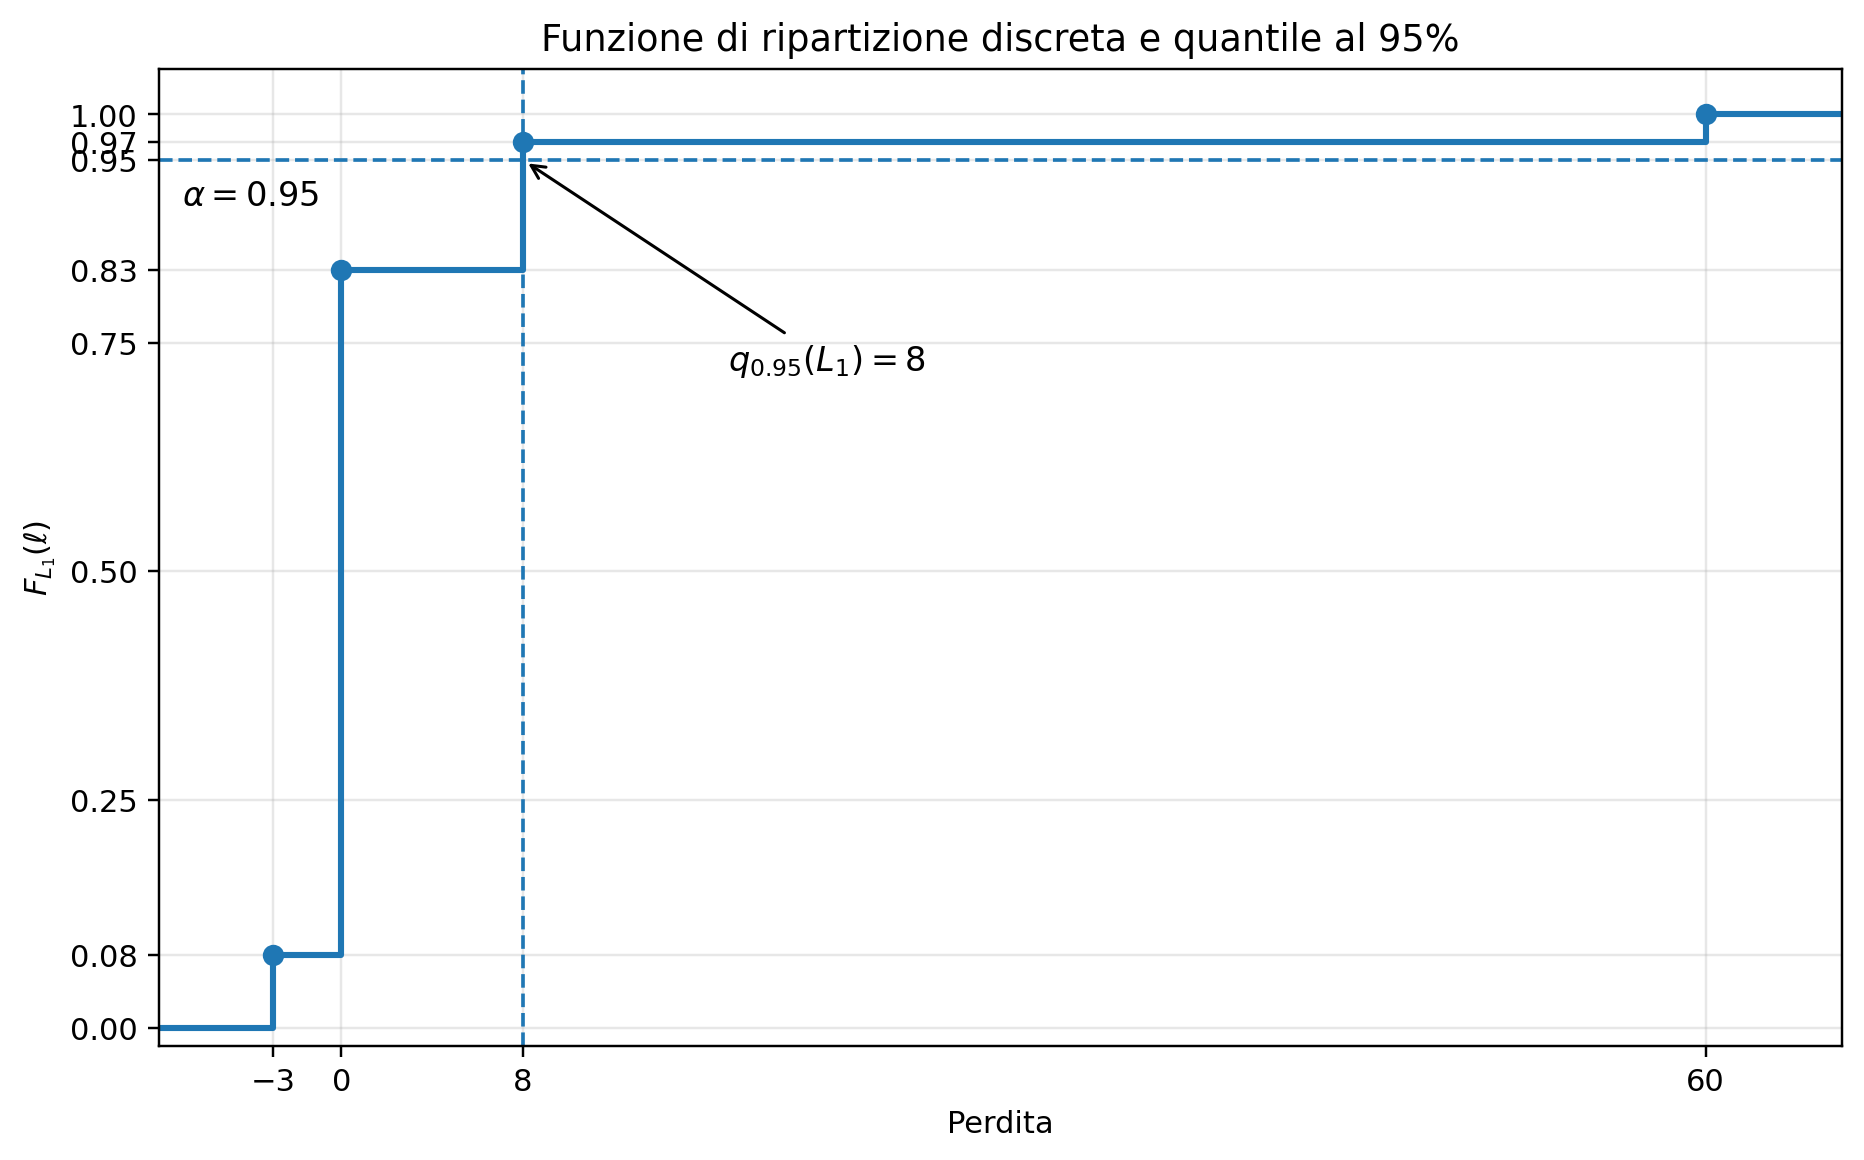
\includegraphics[width=0.82\textwidth]
{../graphics/Cap09_funzione_ripartizione_quantile.png}
\caption{Funzione di ripartizione discreta della perdita e quantile di
livello $0.95$.}
\label{fig:cap09-cdf-quantile}
\end{figure}

La discrezione della distribuzione produce anche variazioni discontinue
del quantile al variare di $\alpha$. Nell'esempio,

\[
q_{\alpha}(L_1\mid X_0=2)
=
\begin{cases}
-3,
&
0<\alpha\leq0.08,
\\[1mm]
0,
&
0.08<\alpha\leq0.83,
\\[1mm]
8,
&
0.83<\alpha\leq0.97,
\\[1mm]
60,
&
0.97<\alpha<1.
\end{cases}
\]

Il quantile \textbf{rimane costante} per interi intervalli di livelli di
probabilit\`{a} e cambia bruscamente quando $\alpha$ supera una
probabilit\`{a} cumulata.

Ad esempio,

\[
q_{0.97}(L_1\mid X_0=2)=8,
\]

mentre, per ogni valore anche di poco superiore a $0.97$,

\[
q_{\alpha}(L_1\mid X_0=2)=60.
\]

Una variazione molto piccola del livello di confidenza pu\`{o} quindi
produrre una variazione molto ampia della soglia monetaria. Questa
instabilit\`{a} non costituisce un errore di calcolo: \`{e} una
conseguenza della distribuzione discreta e della ridotta massa di
probabilit\`{a} collocata tra le perdite intermedie e il default.

\begin{remark}
Per calcolare correttamente un quantile discreto occorre:

\begin{enumerate}

\item ordinare le realizzazioni di $L_h$ in senso crescente;

\item associare a ciascuna realizzazione la relativa probabilit\`{a};

\item costruire le probabilit\`{a} cumulate nell'ordine delle perdite;

\item selezionare la prima perdita per la quale la probabilit\`{a}
cumulata raggiunge o supera $\alpha$.

\end{enumerate}
\end{remark}

L'ordinamento deve riguardare le perdite monetarie, non i codici
numerici attribuiti agli stati della catena. Inoltre, la convenzione

\[
q_{\alpha}(L)
=
\inf
\{
\ell:F_L(\ell)\geq\alpha
\}
\]

deve essere dichiarata esplicitamente. In presenza di distribuzioni
discrete, definizioni o algoritmi differenti possono trattare in modo
diverso i punti nei quali $\alpha$ coincide con una probabilit\`{a}
cumulata.

Il quantile appena definito fornisce la base matematica del Value at
Risk. Nella sezione successiva, la stessa quantit\`{a} verr\`{a}
interpretata come soglia di perdita associata a un livello di
confidenza e a un orizzonte temporale determinati.

\section{Value at Risk creditizio}

\label{sec:cap9-var-creditizio}

Il quantile introdotto nella sezione precedente pu\`{o} essere
interpretato come una soglia monetaria di rischio. Nel contesto
creditizio, tale soglia viene denominata \emph{Value at Risk} della
perdita.

\subsection{Definizione}

\label{subsec:cap9-definizione-var}

\begin{definition}
Sia $L$ una variabile casuale perdita e sia $\alpha\in(0,1)$. Il
\emph{Value at Risk} di livello $\alpha$ \`{e}

\[
\VaR_{\alpha}(L)
=
q_{\alpha}(L)
=
\inf
\left\{
\ell\in\R:
F_L(\ell)\geq\alpha
\right\}.
\]
\end{definition}

Per definizione,

\[
\Prob
\left(
L\leq\VaR_{\alpha}(L)
\right)
\geq
\alpha.
\]

In una distribuzione discreta, la probabilit\`{a} pu\`{o} essere
strettamente maggiore di $\alpha$, poich\'{e} la funzione di
ripartizione pu\`{o} superare il livello richiesto mediante un salto.

Condizionatamente allo stato iniziale $X_0=i$, indicheremo con

\[
\VaR_{\alpha,i}(h)
=
q_{\alpha}(L_h\mid X_0=i)
\]

il VaR della perdita creditizia all'orizzonte $h$.

Nell'esempio della Sezione~9.6,

\[
\VaR_{0.95,2}(1)=8,
\]

poich\'{e}

\[
\Prob(L_1\leq0\mid X_0=2)=0.83<0.95
\]

e

\[
\Prob(L_1\leq8\mid X_0=2)=0.97\geq0.95.
\]

Il risultato indica che $8$ \`{e} la pi\`{u} piccola soglia di perdita
per la quale la probabilit\`{a} cumulata raggiunge almeno il $95\%$.

\subsection{Orizzonte e livello di confidenza}

\label{subsec:cap9-orizzonte-confidenza-var}

Un valore di VaR non \`{e} interpretabile senza specificare almeno:

\begin{itemize}

\item l'orizzonte temporale $h$;

\item il livello di confidenza $\alpha$;

\item la valuta o l'unit\`{a} monetaria della perdita;

\item la distribuzione di $L_h$ e il modello utilizzato per
costruirla.

\end{itemize}

Ad esempio, l'affermazione

\begin{quote}
\emph{il VaR \`{e} pari a 8}
\end{quote}

\noindent
\`{e} incompleta. Una formulazione corretta \`{e}:

\begin{quote}
\emph{Il VaR al $95\%$ della perdita a un anno, condizionatamente al
rating iniziale $i=2$, \`{e} pari a 8 unit\`{a} monetarie nel modello
di transizione del rating considerato.}
\end{quote}

Una variazione dell'orizzonte modifica sia le probabilit\`{a} degli
stati futuri, attraverso $P^h$, sia i valori associati ai rating,
attraverso la funzione $\ell(j,h)$. Pertanto,

\[
\VaR_{\alpha,i}(h)
\]

dipende congiuntamente dal modello delle transizioni e dal modello
delle conseguenze economiche.

\subsection{Credit VaR ed economic capital}

\label{subsec:cap9-credit-var-capitale}

L'espressione \emph{Credit VaR} non viene utilizzata in modo
perfettamente uniforme. Essa pu\`{o} indicare:

\begin{itemize}

\item il quantile della distribuzione della perdita totale;

\item la perdita inattesa quantilica, ottenuta sottraendo la perdita
attesa dal quantile.

\end{itemize}

Nel presente capitolo adotteremo la seguente convenzione:

\[
\mathrm{CreditVaR}_{\alpha,i}(h)
=
\VaR_{\alpha,i}(h),
\]

ossia il Credit VaR coincide con il quantile della perdita totale.

Il capitale economico associato al livello $\alpha$ viene invece
definito come

\[
\mathrm{EC}_{\alpha,i}(h)
=
\VaR_{\alpha,i}(h)
-
\mathrm{EL}_i(h).
\]

La distinzione \`{e} quindi

\[
\begin{array}{lll}
\VaR_{\alpha,i}(h)
&
&
\text{perdita corrispondente al quantile $\alpha$,}
\\[2mm]
\mathrm{EL}_i(h)
&
&
\text{perdita media,}
\\[2mm]
\mathrm{EC}_{\alpha,i}(h)
&
&
\text{perdita quantilica eccedente la media.}
\end{array}
\]

Nell'esempio precedente,

\[
\mathrm{EL}_2(1)=2.68
\]

e

\[
\VaR_{0.95,2}(1)=8.
\]

Pertanto,

\[
\mathrm{EC}_{0.95,2}(1)
=
8-2.68
=
5.32.
\]

Il valore $5.32$ rappresenta la distanza tra la soglia di perdita al
$95\%$ e il costo medio probabilistico dell'esposizione.

\subsection{Limiti del VaR}

\label{subsec:cap9-limiti-var}

Il VaR fornisce una soglia monetaria associata a un livello di
confidenza e a un orizzonte temporale. Questa immediatezza ne facilita
l'interpretazione e la comunicazione, ma non deve nascondere alcuni
limiti importanti.

\medskip

\noindent
\textbf{Il VaR non rappresenta la massima perdita possibile.}

Poniamo

\[
v=\VaR_{\alpha}(L).
\]

Per definizione,

\[
\Prob(L\leq v)\geq\alpha.
\]

Di conseguenza,

\[
\Prob(L>v)\leq 1-\alpha.
\]

Quindi almeno una quota
$1-\alpha$ della distribuzione sar\`{a} associata a perdite superiori a
$v$ e la domanda:

\begin{quote}
\emph{Il VaR costituisce un limite superiore della perdita?}
\end{quote}

\noindent deve ricevere risposta negativa. Il VaR indica una soglia della
distribuzione, non la perdita massima realizzabile.

\medskip

\noindent
\textbf{Il VaR non descrive la severit\`{a} delle perdite oltre la
soglia.}

Una volta determinato il quantile $v$, il VaR non utilizza
l'informazione relativa all'ammontare delle perdite superiori a tale
valore. Se la parte estrema della distribuzione diventa pi\`{u} severa,
ma il quantile di livello $\alpha$ rimane invariato, anche il VaR
rimane invariato.

Due distribuzioni possono pertanto avere lo stesso VaR e presentare
perdite molto differenti negli scenari pi\`{u} sfavorevoli. Il VaR
individua il punto nel quale viene raggiunto il livello di probabilit\`{a}
$\alpha$, ma non misura la gravit\`{a} della coda successiva.

\medskip

\noindent
\textbf{Il VaR pu\`{o} non essere subadditivo.}

Una misura di rischio \`{e} subadditiva se, per due perdite $L_A$ e
$L_B$,

\[
\VaR_{\alpha}(L_A+L_B)
\leq
\VaR_{\alpha}(L_A)
+
\VaR_{\alpha}(L_B).
\]

La propriet\`{a} esprime l'idea che il rischio della posizione
aggregata non debba superare la somma dei rischi misurati separatamente.

Consideriamo ora un esempio autonomo, distinto da quelli sviluppati
nelle sezioni precedenti. Siano $L_A$ e $L_B$ le perdite relative a
due esposizioni indipendenti, entrambe caratterizzate dalla
distribuzione

\[
\begin{array}{c|cc}
\text{perdita}
&
0
&
10
\\
\hline
\text{probabilit\`{a}}
&
0.96
&
0.04
\end{array}
\]

Al livello $\alpha=0.95$,

\[
\VaR_{0.95}(L_A)
=
\VaR_{0.95}(L_B)
=
0,
\]

poich\'{e} per ciascuna esposizione

\[
\Prob(L_A\leq0)
=
\Prob(L_B\leq0)
=
0.96
\geq
0.95.
\]

La perdita aggregata $L_A+L_B$ pu\`{o} assumere i valori $0$, $10$ e
$20$. Per l'indipendenza, la sua distribuzione \`{e}

\[
\begin{array}{c|ccc}
\text{perdita aggregata}
&
0
&
10
&
20
\\
\hline
\text{probabilit\`{a}}
&
(0.96)^2
&
2(0.96)(0.04)
&
(0.04)^2
\\
\hline
&
0.9216
&
0.0768
&
0.0016
\end{array}
\]

La probabilit\`{a} cumulata in corrispondenza della perdita nulla
\`{e}

\[
\Prob(L_A+L_B\leq0)
=
0.9216
<
0.95.
\]

In corrispondenza della perdita $10$ si ha invece

\[
\begin{split}
\Prob(L_A+L_B\leq10)
&=
0.9216+0.0768
\\
&=
0.9984
\geq
0.95.
\end{split}
\]

Pertanto,

\[
\VaR_{0.95}(L_A+L_B)=10.
\]

Ne segue

\[
\VaR_{0.95}(L_A+L_B)
=
10
>
0
=
\VaR_{0.95}(L_A)
+
\VaR_{0.95}(L_B).
\]

In questo esempio il VaR viola la subadditivit\`{a}: la misura
attribuita alla posizione aggregata supera la somma delle misure
attribuite alle due esposizioni considerate separatamente.

\medskip

\noindent
\textbf{Il VaR pu\`{o} essere instabile nelle distribuzioni discrete.}

Torniamo ora alla distribuzione della perdita utilizzata nelle sezioni
precedenti. Le probabilit\`{a} cumulate associate alle perdite $8$ e
$60$ sono rispettivamente

\[
F_{L_1\mid 2}(8)=0.97
\]

e

\[
F_{L_1\mid 2}(60)=1.
\]

Di conseguenza,

\[
\VaR_{0.97,2}(1)=8,
\]

mentre, per ogni $\alpha>0.97$,

\[
\VaR_{\alpha,2}(1)=60.
\]

Un incremento anche molto piccolo del livello di confidenza pu\`{o}
quindi produrre un ampio salto della soglia monetaria. Questo
comportamento deriva dai salti della funzione di ripartizione e dalla
massa di probabilit\`{a} associata al default.

I limiti esaminati mostrano che il VaR non contiene tutta
l'informazione necessaria per valutare il rischio della coda. In
particolare, non misura l'ammontare medio delle perdite pi\`{u}
sfavorevoli. Questa informazione sar\`{a} fornita dalil CVaR, o
Expected Shortfall.

\section{CVaR ed Expected Shortfall}

\label{sec:cap9-cvar-expected-shortfall}

Il VaR individua una soglia della distribuzione, ma non descrive la
gravit\`{a} delle perdite che la superano. Per misurare anche la
severit\`{a} della coda si introduce il CVaR, normalmente denominato
anche \emph{Expected Shortfall}.

\subsection{Definizione mediante quantili}

\label{subsec:cap9-definizione-cvar}

\begin{definition}
Sia $L$ una variabile casuale perdita e sia $\alpha\in(0,1)$. Il
\emph{Conditional Value at Risk} di livello $\alpha$ \`{e}

\[
\CVaR_{\alpha}(L)
=
\frac{1}{1-\alpha}
\int_{\alpha}^{1}
q_u(L)\,du.
\]
\end{definition}

Il CVaR rappresenta la media dei quantili appartenenti alla frazione
$1-\alpha$ pi\`{u} sfavorevole della distribuzione.

Nel presente corso adotteremo la convenzione

\[
\operatorname{ES}_{\alpha}(L)
=
\CVaR_{\alpha}(L),
\]

utilizzando quindi \emph{Expected Shortfall} e CVaR come denominazioni
della stessa misura di rischio.

Per una perdita all'orizzonte $h$, condizionatamente allo stato
iniziale $X_0=i$, scriveremo

\[
\CVaR_{\alpha,i}(h)
=
\CVaR_{\alpha}(L_h\mid X_0=i).
\]

A differenza del VaR, Il CVaR dipende non soltanto dal punto in cui
inizia la coda, ma anche dall'ampiezza delle perdite che la
costituiscono.

\subsection{Rappresentazione di ottimizzazione}

\label{subsec:cap9-rappresentazione-ottimizzazione-cvar}

Il CVaR ammette la rappresentazione

\[
\boxed{
\CVaR_{\alpha}(L)
=
\min_{\eta\in\R}
\left\{
\eta
+
\frac{1}{1-\alpha}
\E\left[(L-\eta)^+\right]
\right\},
}
\]

dove

\[
(x)^+
=
\max\{x,0\}.
\]

Per un valore assegnato di $\eta$, il termine

\[
(L-\eta)^+
\]

misura soltanto l'eccesso della perdita rispetto alla soglia $\eta$.
Le realizzazioni inferiori alla soglia non producono alcun contributo.

La funzione

\[
\eta
\longmapsto
\eta
+
\frac{1}{1-\alpha}
\E\left[(L-\eta)^+\right]
\]

\`{e} convessa. Un suo minimizzatore pu\`{o} essere scelto tra i
quantili di livello $\alpha$; nelle distribuzioni discrete il
minimizzatore pu\`{o} non essere unico.

Questa rappresentazione sar\`{a} particolarmente utile quando il CVaR
verr\`{a} inserita nella funzione obiettivo o nei vincoli di un
problema di ottimizzazione.

\subsection{Distribuzioni discrete e massa nel punto di VaR}

\label{subsec:cap9-cvar-discreta}

Nelle distribuzioni continue, sotto opportune condizioni, il CVaR
pu\`{o} essere interpretata come perdita media condizionata al
superamento del VaR. Questa interpretazione non \`{e} generalmente
corretta nelle distribuzioni discrete.

Poniamo

\[
v
=
\VaR_{\alpha}(L).
\]

Se la funzione di ripartizione presenta un salto nel punto $v$, il
livello $\alpha$ pu\`{o} trovarsi all'interno della massa di
probabilit\`{a} associata a $L=v$. In tal caso,

\[
\CVaR_{\alpha}(L)
=
\frac{
v\left[F_L(v)-\alpha\right]
+
\E\left[
L\1_{\{L>v\}}
\right]
}{
1-\alpha
}.
\]

La formula comprende:

\begin{itemize}

\item tutte le perdite strettamente superiori al VaR;

\item soltanto la frazione della massa nel punto di VaR necessaria a
completare la probabilit\`{a} di coda $1-\alpha$.

\end{itemize}

Riprendiamo la distribuzione utilizzata nelle sezioni precedenti:

\[
\begin{array}{c|cccc}
L_1
&
-3
&
0
&
8
&
60
\\
\hline
\Prob(L_1=\ell\mid X_0=2)
&
0.08
&
0.75
&
0.14
&
0.03
\\
\hline
F_{L_1\mid 2}(\ell)
&
0.08
&
0.83
&
0.97
&
1.00
\end{array}
\]

Al livello $\alpha=0.95$, dalla riga della funzione di ripartizione si
osserva che

\[
F_{L_1\mid 2}(0)=0.83<0.95,
\qquad
F_{L_1\mid 2}(8)=0.97\geq0.95.
\]

Pertanto,

\[
\VaR_{0.95,2}(1)=8.
\]

Il CVaR considera la coda pi\`{u} sfavorevole della distribuzione,
avente probabilit\`{a}

\[
1-\alpha=0.05.
\]

La funzione di ripartizione raggiunge il valore $0.97$ in
corrispondenza della perdita $8$. La parte della coda compresa tra i
livelli $0.95$ e $0.97$ ha quindi probabilit\`{a}

\[
F_{L_1\mid 2}(8)-\alpha
=
0.97-0.95
=
0.02
\]

ed \`{e} associata alla perdita $8$.

La parte restante della coda, compresa tra i livelli $0.97$ e $1$, ha
probabilit\`{a}

\[
1-F_{L_1\mid 2}(8)
=
1-0.97
=
0.03
\]

ed \`{e} associata alla perdita $60$.

Normalizzando queste probabilit\`{a} rispetto alla massa complessiva
della coda, si ottengono le probabilit\`{a} condizionate

\[
\frac{0.02}{0.05}=0.40,
\qquad
\frac{0.03}{0.05}=0.60.
\]

Il CVaR \`{e} quindi il valore atteso condizionato alla coda
pi\`{u} sfavorevole di probabilit\`{a} $0.05$:

\[
\begin{split}
\CVaR_{0.95,2}(1)
&=
8\left(\frac{0.02}{0.05}\right)
+
60\left(\frac{0.03}{0.05}\right)
\\
&=
39.2.
\end{split}
\]

La probabilit\`{a} $0.02$ rappresenta la parte della massa collocata
nel punto di VaR che deve essere inclusa per completare la coda di
probabilit\`{a} $0.05$. Non viene quindi utilizzata l'intera
probabilit\`{a} $0.14$ associata alla perdita $8$.

Per questo motivo, nelle distribuzioni discrete il CVaR non coincide
in generale con

\[
\E
\left[
L_1
\mid
L_1\geq\VaR_{0.95}(L_1)
\right],
\]

poich\'{e} tale condizionamento includerebbe tutta la massa collocata
nel punto di VaR, anzich\'{e} soltanto la frazione necessaria a
costruire la coda di probabilit\`{a} $1-\alpha$.

Lo stesso risultato si ottiene dalla rappresentazione di
ottimizzazione, ponendo $\eta=8$:

\[
\begin{split}
\CVaR_{0.95,2}(1)
&=
8
+
\frac{1}{0.05}
\E\left[(L_1-8)^+\mid X_0=2\right]
\\
&=
8
+
\frac{1}{0.05}(60-8)(0.03)
\\
&=
39.2.
\end{split}
\]

Non sarebbe invece corretto calcolare semplicemente

\[
\E[L_1\mid L_1\geq8,\ X_0=2].
\]

Infatti,

\[
\begin{split}
\E[L_1\mid L_1\geq8,\ X_0=2]
&=
\frac{
(8)(0.14)+(60)(0.03)
}{
0.14+0.03
}
\\
&\approx
17.18,
\end{split}
\]

che non coincide con il CVaR. Il condizionamento $L_1\geq8$ include
l'intera massa di probabilit\`{a} associata alla perdita $8$, mentre
la coda al $5\%$ ne richiede soltanto una parte.

In generale, quindi,

\[
\boxed{
\CVaR_{\alpha}(L)
\neq
\E
\left[
L\mid L\geq\VaR_{\alpha}(L)
\right]
}
\]

quando la distribuzione presenta una massa nel punto di VaR.

\subsection{Confronto tra VaR e CVaR}

\label{subsec:cap9-confronto-var-cvar}

Consideriamo due distribuzioni di perdita:

\[
\begin{array}{c|cccc}
&
0
&
10
&
20
&
100
\\
\hline
\Prob(L_A=x)
&
0.95
&
0
&
0.05
&
0
\\
\Prob(L_B=x)
&
0.95
&
0.04
&
0
&
0.01
\end{array}
\]

Per entrambe le distribuzioni,

\[
\Prob(L_A\leq0)
=
\Prob(L_B\leq0)
=
0.95.
\]

Pertanto,

\[
\VaR_{0.95}(L_A)
=
\VaR_{0.95}(L_B)
=
0.
\]

Il VaR non distingue quindi le due esposizioni. Le rispettive code
sono per\`{o} differenti.

Per $L_A$, l'intera coda al $5\%$ \`{e} costituita dalla perdita $20$:

\[
\CVaR_{0.95}(L_A)
=
20.
\]

Per $L_B$, la coda comprende una perdita pari a $10$ con probabilit\`{a}
$0.04$ e una perdita pari a $100$ con probabilit\`{a} $0.01$:

\[
\begin{split}
\CVaR_{0.95}(L_B)
&=
\frac{
(10)(0.04)+(100)(0.01)
}{
0.05
}
\\
&=
28.
\end{split}
\]

Si ottiene quindi

\[
\VaR_{0.95}(L_A)
=
\VaR_{0.95}(L_B),
\]

ma

\[
\CVaR_{0.95}(L_A)
<
\CVaR_{0.95}(L_B).
\]

Le due distribuzioni iniziano la propria coda nello stesso punto, ma
$L_B$ presenta perdite estreme pi\`{u} severe. Il VaR individua
soltanto la soglia; il CVaR utilizza anche l'informazione contenuta
oltre tale soglia.

\section{Applicazione integrata: rischio di una singola esposizione}

\label{sec:cap9-applicazione-singola-esposizione}

Le sezioni precedenti hanno introdotto separatamente le probabilit\`{a}
di transizione, la funzione di perdita e le misure di rischio. In
questa sezione gli stessi elementi vengono riuniti in un'unica
applicazione finanziaria.

Riprendiamo la matrice di transizione annuale dei rating introdotta nel
Capitolo~8:

\[
P_R
=
\begin{pmatrix}
0.80 & 0.18 & 0.02 & 0.00\\
0.08 & 0.75 & 0.14 & 0.03\\
0.02 & 0.18 & 0.65 & 0.15\\
0.00 & 0.00 & 0.00 & 1.00
\end{pmatrix},
\]

con stati

\[
\mathcal{I}
=
\{
1=\text{alta qualit\`{a}},
\,
2=\text{qualit\`{a} intermedia},
\,
3=\text{speculative grade},
\,
D=\text{default}
\}.
\]

Lo stato $D$, equivalente allo stato $4$ del Capitolo~8, \`{e}
assorbente. Consideriamo un'obbligazione emessa da un soggetto
inizialmente appartenente alla classe di qualit\`{a} intermedia e
valutiamo il rischio a un anno.

\subsection{Probabilit\`{a} degli stati futuri}

\label{subsec:cap9-applicazione-probabilita-stati}

Lo stato iniziale \`{e}

\[
X_0=2.
\]

Poich\'{e} l'orizzonte \`{e} $h=1$, la distribuzione dei rating futuri
si legge direttamente nella seconda riga di $P_R$:

\[
\Prob(X_1=j\mid X_0=2)
=
\begin{cases}
0.08, & j=1,\\[1mm]
0.75, & j=2,\\[1mm]
0.14, & j=3,\\[1mm]
0.03, & j=D.
\end{cases}
\]

La probabilit\`{a} di default entro un anno coincide con la
probabilit\`{a} marginale di default nel primo periodo:

\[
\mathrm{PD}_{2}^{\mathrm{cum}}(1)
=
\mathrm{PD}_{2}^{\mathrm{marg}}(1)
=
(P_R)_{2D}
=
0.03.
\]

La sola probabilit\`{a} di default non descrive tuttavia l'intera
distribuzione economica dell'esposizione. Con probabilit\`{a} $0.14$
l'emittente subisce un downgrade senza entrare in default, mentre con
probabilit\`{a} $0.08$ ottiene un miglioramento del rating.

\subsection{Valori e perdite per stato}

\label{subsec:cap9-applicazione-valori-perdite}

Consideriamo un'obbligazione con

\[
N=100,
\qquad
C=4,
\qquad
T=5,
\]

dove $N$ \`{e} il valore nominale, $C$ la cedola annuale e $T$ la
scadenza. La valutazione viene effettuata alla data $h=1$,
immediatamente dopo il pagamento della prima cedola; rimangono quindi
quattro pagamenti cedolari e il rimborso finale del capitale.

Assumiamo una struttura piatta dei tassi privi di rischio con

\[
r=0.02
\]

e tassi spread creditizi dipendenti dal rating futuro:

\[
s_1=0.012,
\qquad
s_2=0.020,
\qquad
s_3=0.043.
\]

Il tasso di sconto utilizzato per valutare l'obbligazione nello stato
non-default $j$ \`{e}

\[
y_j=r+s_j.
\]

Il valore condizionato al rating futuro \`{e} quindi

\[
V_j(1)
=
\sum_{k=1}^{4}
\frac{C}{(1+y_j)^k}
+
\frac{N}{(1+y_j)^4},
\qquad
j=1,2,3.
\]

Si ottiene

\[
V_1(1)\approx102.96,
\qquad
V_2(1)=100,
\qquad
V_3(1)\approx92.08.
\]

L'aumento dello spread associato al downgrade riduce il valore
dell'obbligazione anche in assenza di default.

Per lo stato di default assumiamo un recovery rate pari al $40\%$
dell'esposizione:

\[
R=0.40,
\qquad
\mathrm{EAD}_1=100.
\]

Assumendo che il recupero sia disponibile alla data di valutazione, il
valore nello stato di default \`{e}

\[
V_D(1)
=
R \cdot \mathrm{EAD}_1
=
40.
\]

Assumiamo come valore di riferimento il valore corrispondente alla
permanenza nella classe iniziale:

\[
V^{\mathrm{ref}}(1)
=
V_2(1)
=
100.
\]

La funzione di perdita \`{e}

\[
\ell(j,1)
=
V^{\mathrm{ref}}(1)-V_j(1).
\]

I risultati sono riassunti nella tabella seguente:

\[
\begin{array}{cccccc}
\hline
\text{stato}
&
(P_R)_{2j}
&
s_j
&
y_j
&
V_j(1)
&
\ell(j,1)
\\
\hline
1
&
0.08
&
1.20\%
&
3.20\%
&
102.96
&
-2.96
\\
2
&
0.75
&
2.00\%
&
4.00\%
&
100.00
&
0.00
\\
3
&
0.14
&
4.30\%
&
6.30\%
&
92.08
&
7.92
\\
D
&
0.03
&
--
&
--
&
40.00
&
60.00
\\
\hline
\end{array}
\]

Per mantenere leggibili i calcoli e raccordare l'applicazione agli
esempi delle sezioni precedenti, utilizziamo i valori arrotondati

\[
\ell(1,1)=-3,
\qquad
\ell(2,1)=0,
\qquad
\ell(3,1)=8,
\qquad
\ell(D,1)=60.
\]

Le misure che seguono sono calcolate sui valori arrotondati. L'impiego
dei valori non arrotondati produrrebbe differenze numeriche minime,
senza modificare l'ordinamento delle perdite o la loro interpretazione
economica.

\subsection{Distribuzione completa della perdita}

\label{subsec:cap9-applicazione-distribuzione-perdita}

La perdita a un anno \`{e}

\[
L_1
=
\ell(X_1,1).
\]

Condizionatamente al rating iniziale $X_0=2$, la funzione di massa e la
funzione di ripartizione sono:

\[
\begin{array}{c|cccc}
L_1
&
-3
&
0
&
8
&
60
\\
\hline
\Prob(L_1=\ell\mid X_0=2)
&
0.08
&
0.75
&
0.14
&
0.03
\\
\hline
F_{L_1\mid 2}(\ell)
&
0.08
&
0.83
&
0.97
&
1.00
\end{array}
\]

La distribuzione contiene quattro conseguenze economiche distinte:

\[
\begin{array}{lll}
L_1=-3
&
&
\text{guadagno da miglioramento del rating,}
\\[1mm]
L_1=0
&
&
\text{assenza di variazione rispetto al riferimento,}
\\[1mm]
L_1=8
&
&
\text{perdita mark-to-market da downgrade,}
\\[1mm]
L_1=60
&
&
\text{perdita da default al netto del recupero.}
\end{array}
\]

La probabilit\`{a} cumulata raggiunge $0.83$ in corrispondenza della
perdita nulla e $0.97$ in corrispondenza della perdita $8$. Il default
occupa la parte estrema della coda, con probabilit\`{a} $0.03$.

\subsection{Misure di rischio}

\label{subsec:cap9-applicazione-misure-rischio}

La perdita attesa \`{e}

\[
\begin{split}
\mathrm{EL}_2(1)
&=
\E[L_1\mid X_0=2]
\\
&=
(-3)(0.08)
+
(0)(0.75)
+
(8)(0.14)
+
(60)(0.03)
\\
&=
2.68.
\end{split}
\]

Il secondo momento \`{e}

\[
\begin{split}
\E[L_1^2\mid X_0=2]
&=
(-3)^2(0.08)
+
8^2(0.14)
+
60^2(0.03)
\\
&=
117.68.
\end{split}
\]

Pertanto,

\[
\begin{split}
\Var(L_1\mid X_0=2)
&=
117.68-(2.68)^2
\\
&=
110.4976,
\end{split}
\]

e la deviazione standard \`{e}

\[
\sigma_{L,2}(1)
=
\sqrt{110.4976}
\approx
10.51.
\]

Consideriamo ora il livello di confidenza

\[
\alpha=0.95.
\]

Poich\'{e}

\[
F_{L_1\mid 2}(0)=0.83<0.95
\]

e

\[
F_{L_1\mid 2}(8)=0.97\geq0.95,
\]

si ottiene

\[
\VaR_{0.95,2}(1)=8.
\]

Per il calcolo del CVaR, la coda pi\`{u} sfavorevole deve avere
probabilit\`{a} $0.05$. La perdita $60$ occupa una massa pari a
$0.03$; la parte compresa tra i livelli cumulati $0.95$ e $0.97$,
pari a $0.02$, \`{e} associata alla perdita $8$. Normalizzando rispetto
alla probabilit\`{a} complessiva della coda,

\[
\begin{split}
\CVaR_{0.95,2}(1)
&=
8\left(\frac{0.02}{0.05}\right)
+
60\left(\frac{0.03}{0.05}\right)
\\
&=
39.2.
\end{split}
\]

Infine, il capitale economico quantilico \`{e}

\[
\begin{split}
\mathrm{EC}_{0.95,2}(1)
&=
\VaR_{0.95,2}(1)
-
\mathrm{EL}_2(1)
\\
&=
8-2.68
\\
&=
5.32.
\end{split}
\]

Le misure ottenute possono essere raccolte nel prospetto seguente:

\[
\begin{array}{lc}
\hline
\text{misura}
&
\text{valore}
\\
\hline
\mathrm{EL}_2(1)
&
2.68
\\
\Var(L_1\mid X_0=2)
&
110.4976
\\
\sigma_{L,2}(1)
&
10.51
\\
\VaR_{0.95,2}(1)
&
8
\\
\CVaR_{0.95,2}(1)
&
39.2
\\
\mathrm{EC}_{0.95,2}(1)
&
5.32
\\
\hline
\end{array}
\]

\subsection{Interpretazione}

\label{subsec:cap9-applicazione-interpretazione}

La perdita attesa pu\`{o} essere scomposta nei contributi associati ai
differenti stati futuri. In termini simbolici,

\[
\begin{split}
\mathrm{EL}_2(1)
&=
\sum_{j\in\mathcal{I}}
\ell(j,1)(P_R)_{2j}
\\
&=
\ell(1,1)(P_R)_{21}
+
\ell(2,1)(P_R)_{22}
\\
&\quad
+
\ell(3,1)(P_R)_{23}
+
\ell(D,1)(P_R)_{2D}.
\end{split}
\]

Sostituendo le perdite e le probabilit\`{a} di transizione,

\[
\begin{split}
\mathrm{EL}_2(1)
&=
\underbrace{(-3)(0.08)}_{\text{upgrade}}
+
\underbrace{(0)(0.75)}_{\text{permanenza}}
\\
&\quad
+
\underbrace{(8)(0.14)}_{\text{downgrade}}
+
\underbrace{(60)(0.03)}_{\text{default}} =2.68.
\end{split}
\]

I quattro contributi sono quindi

\[
-0.24,
\qquad
0,
\qquad
1.12,
\qquad
1.80.
\]

Il default fornisce il contributo positivo maggiore alla perdita
attesa, ma non \`{e} l'unica fonte di rischio. Il downgrade genera una
perdita attesa mark-to-market pari a $1.12$, mentre il miglioramento
del rating produce un guadagno atteso pari a $0.24$ e riduce la perdita
media complessiva.

Il VaR al $95\%$ \`{e} pari a $8$. Tale perdita coincide quindi con la perdita prodotta dal downgrade, non con la perdita da default.
Questo accade perch\'{e} la probabilit\`{a} cumulata raggiunge gi\`{a}
il valore $0.97$ in corrispondenza di $L_1=8$.

La perdita da default, pari a $60$, rimane interamente oltre la soglia
del VaR. Il VaR segnala dove inizia la parte pi\`{u} sfavorevole della
distribuzione, ma non riflette direttamente la distanza tra la perdita
$8$ e la perdita estrema $60$.

Il CVaR, pari a $39.2$, incorpora invece la severit\`{a} della coda. La
coda peggiore del $5\%$ comprende tutti i casi di default, che
rappresentano il $3\%$ della distribuzione, e la frazione necessaria
della massa associata al downgrade. Il valore elevato del CVaR rispetto
al VaR mostra l'importanza della perdita da default negli scenari
estremi.

Infine,

\[
\mathrm{EC}_{0.95,2}(1)=5.32
\]

misura la distanza tra la perdita corrispondente al quantile prefissato e la perdita attesa secondo
la convenzione adottata nel capitolo.

L'applicazione mette cos\`{\i} in evidenza l'intera catena logica:

\[
\boxed{
\begin{array}{c}
\text{matrice di transizione dei rating}
\\
\downarrow
\\
\text{valori condizionati agli stati}
\\
\downarrow
\\
\text{distribuzione della perdita}
\\
\downarrow
\\
\text{EL, VaR, CVaR ed economic capital}.
\end{array}
}
\]

La matrice di transizione costituisce lo scheletro probabilistico del
modello; la valutazione dell'obbligazione e il recovery rate ne
determinano le conseguenze monetarie.

\section{Misura fisica e misura risk-neutral}

\label{sec:cap9-misure-probabilita}

La matrice di transizione attribuisce probabilit\`{a} ai possibili
rating futuri. La scelta delle probabilit\`{a} dipende tuttavia dalla
domanda alla quale il modello deve rispondere.

Occorre distinguere tra:

\[
\text{misurazione del rischio}
\]

e

\[
\text{valutazione di mercato}.
\]

Le due analisi utilizzano lo stesso insieme degli stati creditizi e
possono adottare la stessa struttura markoviana, ma richiedono in
generale matrici di transizione differenti.

Supponiamo, per semplicit\`{a}, che sotto entrambe le misure il rating
segua una catena di Markov omogenea. Indicheremo con

\[
P^{\Prob}
\]

la matrice di transizione sotto la misura fisica e con

\[
P^{\Q}
\]

la matrice di transizione sotto la misura risk-neutral.

\subsection{Due domande differenti}

\label{subsec:cap9-due-domande}

La \emph{misurazione del rischio} considera le probabilit\`{a} con cui
gli stati creditizi possono effettivamente realizzarsi. La domanda
principale \`{e}:

\[
\text{quali perdite possono verificarsi e con quali probabilit\`{a}?}
\]

Questa analisi richiede probabilit\`{a} predittive, riferite
all'evoluzione reale del rating dell'emittente. Le misure di perdita
attesa, VaR e CVaR devono pertanto essere calcolate sotto la misura
fisica $\Prob$.

La \emph{valutazione di mercato} risponde invece alla domanda:

\[
\text{qual \`{e} oggi il valore di mercato dei flussi futuri?}
\]

In un modello di pricing coerente con l'assenza di arbitraggio, il
valore viene ottenuto come valore atteso, sotto la misura
risk-neutral $\Q$, dei flussi futuri opportunamente attualizzati.

La distinzione pu\`{o} essere sintetizzata come segue:

\[
\begin{array}{ccl}
\text{misurazione del rischio}
&
\longrightarrow
&
\text{probabilit\`{a} predittive sotto }\Prob,
\\[2mm]
\text{valutazione di mercato}
&
\longrightarrow
&
\text{valori attesi di flussi attualizzati sotto }\Q.
\end{array}
\]

Le probabilit\`{a} risk-neutral non rappresentano necessariamente le
frequenze con cui gli eventi creditizi si realizzeranno. Esse sono
pesi probabilistici utilizzati per riprodurre i prezzi di mercato.

\subsection{Matrice sotto la misura fisica}

\label{subsec:cap9-matrice-fisica}

Indichiamo con

\[
P^{\Prob}
=
\left(
p_{ij}^{\Prob}
\right)_{i,j\in\mathcal{I}}
\]

la matrice di transizione sotto la misura fisica, dove

\[
p_{ij}^{\Prob}
=
\Prob(X_{t+1}=j\mid X_t=i).
\]

Per una catena omogenea,

\[
\Prob(X_h=j\mid X_0=i)
=
\left[
\left(P^{\Prob}\right)^h
\right]_{ij}.
\]

La matrice $P^{\Prob}$ determina quindi la distribuzione predittiva
degli stati futuri. Data la funzione di perdita $\ell(j,h)$, si
ottiene

\[
\Prob
\left(
L_h=\ell(j,h)
\mid X_0=i
\right)
=
\left[
\left(P^{\Prob}\right)^h
\right]_{ij},
\]

quando stati differenti producono perdite differenti. Se pi\`{u}
stati producono la stessa perdita, le corrispondenti probabilit\`{a}
devono essere aggregate.

La perdita attesa sotto la misura fisica \`{e}

\[
\mathrm{EL}_{i}^{\Prob}(h)
=
\E^{\Prob}[L_h\mid X_0=i]
=
\sum_{j\in\mathcal{I}}
\ell(j,h)
\left[
\left(P^{\Prob}\right)^h
\right]_{ij}.
\]

Anche la funzione di ripartizione della perdita viene costruita
utilizzando le probabilit\`{a} fisiche:

\[
F_{L_h\mid i}^{\Prob}(\lambda)
=
\sum_{\substack{j\in\mathcal{I}:\\
\ell(j,h)\leq\lambda}}
\left[
\left(P^{\Prob}\right)^h
\right]_{ij}.
\]

Da questa distribuzione si ricavano

\[
\VaR_{\alpha,i}^{\Prob}(h)
\]

e

\[
\CVaR_{\alpha,i}^{\Prob}(h).
\]

La sequenza concettuale \`{e} dunque

\[
P^{\Prob}
\longrightarrow
\text{distribuzione predittiva dei rating}
\longrightarrow
\text{distribuzione della perdita}
\longrightarrow
\mathrm{EL}^{\Prob},
\VaR^{\Prob},
\CVaR^{\Prob}.
\]

La matrice fisica pu\`{o} essere stimata, ad esempio, mediante le
frequenze storiche delle transizioni osservate. Il suo impiego
richiede tuttavia cautela, poich\'{e} le frequenze passate possono
non rappresentare correttamente la dinamica futura in presenza di
cambiamenti macroeconomici, istituzionali o nella composizione degli
emittenti.

\subsection{Matrice sotto la misura risk-neutral}

\label{subsec:cap9-matrice-risk-neutral}

Indichiamo con

\[
P^{\Q}
=
\left(
p_{ij}^{\Q}
\right)_{i,j\in\mathcal{I}}
\]

la matrice di transizione sotto la misura risk-neutral, dove

\[
p_{ij}^{\Q}
=
\Q(X_{t+1}=j\mid X_t=i).
\]

Per una catena omogenea sotto $\Q$,

\[
\Q(X_h=j\mid X_0=i)
=
\left[
\left(P^{\Q}\right)^h
\right]_{ij}.
\]

La matrice $P^{\Q}$ non viene utilizzata per prevedere le frequenze
future dei rating. Essa fornisce i pesi probabilistici impiegati nella
valutazione di mercato dei flussi creditizi.

Sia $C_t$ il flusso aleatorio pagato alla data $t$ e sia $D(0,t)$ il
fattore di attualizzazione dalla data $t$ alla data iniziale. Il valore
di mercato al tempo zero \`{e}

\[
V_0
=
\E^{\Q}
\left[
\sum_{t=1}^{T}
D(0,t)C_t
\right].
\]

Nel caso semplificato in cui il fattore di attualizzazione sia
deterministico e il flusso alla data $t$ dipenda soltanto dallo stato
occupato, ossia

\[
C_t=c_t(X_t),
\]

si ottiene

\[
V_0
=
\sum_{t=1}^{T}
D(0,t)
\sum_{j\in\mathcal{I}}
c_t(j)
\left[
\left(P^{\Q}\right)^t
\right]_{ij}.
\]

La struttura rilevante per il pricing \`{e} quindi

\[
P^{\Q}
\longrightarrow
\text{probabilit\`{a} risk-neutral dei flussi}
\longrightarrow
\E^{\Q}
\left[
\text{flussi attualizzati}
\right]
\longrightarrow
\text{valore di mercato}.
\]

In generale,

\[
P^{\Prob}
\neq
P^{\Q}.
\]

Le probabilit\`{a} fisiche riflettono la dinamica predittiva degli
stati creditizi. Le probabilit\`{a} risk-neutral incorporano invece
anche la remunerazione richiesta dal mercato per l'esposizione al
rischio.

Di conseguenza, una matrice stimata mediante frequenze storiche non
pu\`{o} essere utilizzata automaticamente come matrice di pricing. Il
fatto che una matrice descriva adeguatamente le transizioni osservate
non implica che, utilizzata sotto $\Q$, essa riproduca i prezzi delle
obbligazioni creditizie o dei derivati di credito.

\subsection{Portata e limiti della distinzione}

\label{subsec:cap9-portata-misure}

La distinzione tra $\Prob$ e $\Q$ riguarda innanzitutto il ruolo
attribuito alle probabilit\`{a}:

\[
\begin{array}{ccl}
P^{\Prob}
&
:
&
\text{probabilit\`{a} degli scenari futuri},
\\[2mm]
P^{\Q}
&
:
&
\text{pesi probabilistici per la valutazione di mercato}.
\end{array}
\]

Questa separazione non implica tuttavia che la misurazione del rischio
e la valutazione di mercato siano sempre completamente indipendenti.

In un modello di perdita mark-to-market, le probabilit\`{a} con cui si
raggiungono i rating futuri sono generalmente determinate sotto la
misura fisica:

\[
\Prob(X_h=j\mid X_0=i)
=
\left[
\left(P^{\Prob}\right)^h
\right]_{ij}.
\]

Il valore dell'esposizione condizionato allo stato futuro $j$ pu\`{o}
invece essere un valore di mercato, ottenuto alla data $h$ mediante una
valutazione risk-neutral dei flussi successivi. In tal caso,

\[
P^{\Prob}
\longrightarrow
\text{probabilit\`{a} degli scenari},
\]

mentre

\[
P^{\Q}
\longrightarrow
V_j(h).
\]

La perdita all'orizzonte rimane

\[
L_h
=
V^{\mathrm{ref}}(h)-V_{X_h}(h),
\]

ma la sua distribuzione utilizza le probabilit\`{a} fisiche degli
stati, mentre i valori $V_j(h)$ possono incorporare una valutazione di
mercato sotto $\Q$.

Nel seguito assumeremo che la matrice $P^{\Q}$ sia assegnata. La sua
calibrazione a partire dai prezzi di obbligazioni, CDS e altri
strumenti creditizi richiede la specificazione congiunta dei tassi di
interesse, dei flussi contrattuali, del recovery rate e dei premi per
il rischio.

Tali problemi di calibrazione vengono rinviati a corsi specialistici.
Nel presente capitolo la distinzione essenziale \`{e} la seguente:

\[
\boxed{
\begin{array}{c}
P^{\Prob}
\text{ per misurare il rischio,}
\\[2mm]
P^{\Q}
\text{ per valutare i flussi di mercato.}
\end{array}
}
\]

\section{Il credit default swap}

\label{sec:cap9-cds}

La distinzione tra misura fisica e misura risk-neutral diventa
operativa nella valutazione dei derivati di credito. Consideriamo il
\emph{credit default swap}, o CDS, nella sua forma pi\`{u} semplice.

Il CDS \`{e} un contratto nel quale una parte (tipicamente il proprietario di titoli obbligazionari) acquista protezione
contro il verificarsi di un evento creditizio avverso che colpisce l'emittente dei titoli posseduti. In cambio della protezione, essa paga periodicamente un
premio alla controparte.

La valutazione del contratto viene effettuata sotto la misura
risk-neutral $\Q$. Le probabilit\`{a} di default utilizzate nel pricing
sono pertanto ricavate dalla matrice di transizione $P^{\Q}$, non dalla
matrice fisica $P^{\Prob}$.

\subsection{Struttura contrattuale}

\label{subsec:cap9-cds-struttura}

Le parti e gli elementi essenziali di un CDS sono:

\begin{itemize}

\item il \emph{protection buyer}, che acquista la protezione e paga il
premio periodico;

\item il \emph{protection seller}, che riceve i premi e si impegna a
effettuare il pagamento di protezione in caso di evento creditizio;

\item la \emph{reference entity}, ossia l'emittente al cui rischio di
credito \`{e} riferito il contratto;

\item il nozionale $N$, sul quale vengono calcolati sia i premi sia il
pagamento di protezione;

\item il premio periodico, determinato mediante uno spread contrattuale
$s$;

\item il \emph{credit event}, che nel modello semplificato coincide con
il default della reference entity;

\item il \emph{recovery rate} $R$, che determina la parte del nozionale
recuperabile dopo il default;

\item la \emph{scadenza contrattuale} $H$.

\end{itemize}

I flussi del CDS sono suddivisi in due componenti:

\[
\begin{array}{ccl}
\text{gamba dei premi}
&
:
&
\text{pagamenti effettuati dal protection buyer,}
\\[2mm]
\text{gamba di protezione}
&
:
&
\text{pagamento effettuato dal protection seller in caso di default.}
\end{array}
\]

Indichiamo con $\mathrm{PV}_{\mathrm{prot}}$ il valore attuale della
gamba di protezione e con $\mathrm{PV}_{\mathrm{prem}}(s)$ il valore
attuale della gamba dei premi, calcolata per uno spread contrattuale
$s$.

Dal punto di vista del protection buyer, il valore del CDS alla data
iniziale \`{e} quindi

\[
V_{\mathrm{CDS}}(s)
=
\mathrm{PV}_{\mathrm{prot}}
-
\mathrm{PV}_{\mathrm{prem}}(s).
\]

Per il protection seller i segni dei due flussi sono opposti.

Indichiamo con

\[
\tau_D
=
\inf\{h\geq1:X_h=D\}
\]

il tempo di primo ingresso nello stato di default e con $d_h$ il
fattore deterministico di attualizzazione dalla data $h$ alla data
iniziale.

\subsection{Gamba di protezione}

\label{subsec:cap9-cds-protezione}

Se il default si verifica alla data $h$, il protection seller paga al
protection buyer la perdita sul nozionale:

\[
N(1-R).
\]

Il valore attuale del pagamento condizionato all'evento
$\{\tau_D=h\}$ \`{e}

\[
d_hN(1-R).
\]

Poich\'{e} il pagamento viene effettuato soltanto se il primo ingresso
in default avviene alla data $h$, il valore attuale atteso della gamba
di protezione \`{e}

\[
\mathrm{PV}_{\mathrm{prot}}
=
N(1-R)
\sum_{h=1}^{H}
d_h
\Q(\tau_D=h\mid X_0=i).
\]

Le probabilit\`{a} marginali di default sono ottenute dalla matrice
risk-neutral. Poich\'{e} lo stato $D$ \`{e} assorbente,

\[
\Q(\tau_D\leq h\mid X_0=i)
=
\left[
\left(P^{\Q}\right)^h
\right]_{iD},
\]

e quindi

\[
\Q(\tau_D=h\mid X_0=i)
=
\left[
\left(P^{\Q}\right)^h
\right]_{iD}
-
\left[
\left(P^{\Q}\right)^{h-1}
\right]_{iD}.
\]

La gamba di protezione dipende dunque dalle probabilit\`{a} di primo
ingresso in default alle diverse date contrattuali, dal recovery rate
e dai fattori di attualizzazione.

\subsection{Gamba dei premi}

\label{subsec:cap9-cds-premi}

Il protection buyer paga a ogni data $h$ un premio pari a

\[
sN,
\]

purch\'{e} la reference entity sia ancora sopravvissuta oltre tale
data.

Nella convenzione temporale adottata, se il default si verifica
esattamente alla data $h$, il pagamento del premio alla stessa data
non viene effettuato. Il premio alla data $h$ viene quindi pagato
soltanto sull'evento

\[
\{\tau_D>h\}.
\]

Il valore attuale atteso della gamba dei premi \`{e}

\[
\mathrm{PV}_{\mathrm{prem}}(s)
=
sN
\sum_{h=1}^{H}
d_h
\Q(\tau_D>h\mid X_0=i).
\]

Le probabilit\`{a} di sopravvivenza sotto la misura risk-neutral sono

\[
\Q(\tau_D>h\mid X_0=i)
=
1-
\left[
\left(P^{\Q}\right)^h
\right]_{iD}.
\]

Pertanto,

\[
\mathrm{PV}_{\mathrm{prem}}(s)
=
sN
\sum_{h=1}^{H}
d_h
\left\{
1-
\left[
\left(P^{\Q}\right)^h
\right]_{iD}
\right\}.
\]

Il premio contrattuale viene moltiplicato per probabilit\`{a} di
sopravvivenza, poich\'{e} i pagamenti futuri cessano dopo il default
della reference entity.

\subsection{Premio equo del CDS}

\label{subsec:cap9-cds-premio-equilibrio}

Alla data iniziale, il premio equo $s^{*}$ rende nullo il valore del
CDS. Dal punto di vista del protection buyer, deve quindi valere

\[
V_{\mathrm{CDS}}(s^{*})=0,
\]

ossia

\[
\mathrm{PV}_{\mathrm{prem}}(s^{*})
=
\mathrm{PV}_{\mathrm{prot}}.
\]

Sostituendo le espressioni delle due gambe,

\[
s^{*}N
\sum_{h=1}^{H}
d_h
\Q(\tau_D>h\mid X_0=i)
=
N(1-R)
\sum_{h=1}^{H}
d_h
\Q(\tau_D=h\mid X_0=i).
\]

Il nozionale compare in entrambe le gambe e si semplifica. Il premio
equo \`{e} quindi

\[
s^{*}
=
(1-R)
\frac{
\displaystyle
\sum_{h=1}^{H}
d_h
\Q(\tau_D=h\mid X_0=i)
}{
\displaystyle
\sum_{h=1}^{H}
d_h
\Q(\tau_D>h\mid X_0=i)
}.
\]

Il numeratore rappresenta il valore attuale risk-neutral della perdita
unitaria attesa da default:

\[
(1-R)
\sum_{h=1}^{H}
d_h
\Q(\tau_D=h\mid X_0=i).
\]

Il denominatore rappresenta invece il valore attuale atteso di
un'unit\`{a} di premio pagata alle date nelle quali l'emittente
sopravvive:

\[
\sum_{h=1}^{H}
d_h
\Q(\tau_D>h\mid X_0=i).
\]

Il premio equo aumenta, a parit\`{a} delle altre condizioni, quando
aumentano le probabilit\`{a} risk-neutral di default o quando
diminuisce il recovery rate.

La relazione pu\`{o} essere sintetizzata come

\[
\boxed{
\text{premio equo}
=
\frac{
\text{valore attuale atteso della protezione}
}{
\text{valore attuale atteso dell'unit\`{a} di premio}
}.
}
\]

\subsection{Ipotesi semplificatrici}

\label{subsec:cap9-cds-ipotesi}

La formulazione precedente ha finalit\`{a} didattica e si basa sulle
seguenti ipotesi:

\begin{itemize}

\item le date di pagamento e di possibile default sono annuali;

\item i tassi di interesse e i fattori di attualizzazione $d_h$ sono
deterministici;

\item il recovery rate $R$ \`{e} costante;

\item il pagamento della protezione avviene alla data discreta nella
quale viene rilevato il default;

\item non viene corrisposto il premio maturato tra l'ultima data di
pagamento e la data di default;

\item se il default avviene alla data $h$, il premio previsto alla
stessa data non viene pagato;

\item il protection seller \`{e} privo di rischio di controparte;

\item non sono considerati collateral, margini, costi di transazione o
altri aggiustamenti di valutazione.

\end{itemize}

Nei contratti di mercato i premi sono normalmente pagati con frequenza
inferiore all'anno, il default pu\`{o} verificarsi tra due date di
pagamento e il premio maturato deve essere trattato esplicitamente.
Questi elementi modificano il dettaglio dei flussi, ma non la logica
fondamentale del pricing:

\[
\text{valore della gamba dei premi}
=
\text{valore della gamba di protezione}.
\]

La matrice $P^{\Q}$ collega quindi la dinamica risk-neutral dei rating
al valore del CDS:

\[
\boxed{
P^{\Q}
\longrightarrow
\begin{array}{c}
\text{probabilit\`{a} di default}
\\
\text{e di sopravvivenza}
\end{array}
\longrightarrow
\begin{array}{c}
\text{gamba di protezione}
\\
\text{e gamba dei premi}
\end{array}
\longrightarrow
s^{*}.
}
\]

\section{Copertura mediante CDS e rischio residuo}

\label{sec:cap9-copertura-cds}

Un CDS pu\`{o} essere utilizzato per ridurre le perdite associate al
default di un'esposizione creditizia. La copertura non elimina tuttavia
necessariamente tutte le componenti del rischio: il risultato dipende
dal nozionale protetto, dalla scadenza, dalla definizione contrattuale
del credit event e dalla relazione tra il valore dell'esposizione e
quello del CDS.

La distinzione tra misura fisica e misura risk-neutral rimane
essenziale. Il premio del CDS viene determinato mediante probabilit\`{a}
risk-neutral, mentre la distribuzione delle perdite della posizione
coperta deve essere valutata mediante probabilit\`{a} fisiche.

Tutte le componenti monetarie considerate nel seguito sono espresse
alla medesima data di valutazione.

\subsection{Posizione non coperta}

\label{subsec:cap9-posizione-non-coperta}

Indichiamo con $L^{\mathrm{credito}}$ la perdita dell'esposizione
creditizia in assenza di strumenti di copertura.

La perdita della posizione non coperta \`{e} quindi

\[
L^{\mathrm{unhedged}}
=
L^{\mathrm{credito}}.
\]

La sua distribuzione dipende dalle probabilit\`{a} fisiche degli stati
creditizi futuri e dalla funzione che associa a ogni stato il valore
dell'esposizione.

Nel caso dell'applicazione della Sezione~9.9,

\[
L^{\mathrm{unhedged}}
\in
\{-3,0,8,60\},
\]

con distribuzione

\[
\begin{array}{c|cccc}
L^{\mathrm{unhedged}}
&
-3
&
0
&
8
&
60
\\
\hline
\Prob
\left(
L^{\mathrm{unhedged}}=\ell
\mid X_0=2
\right)
&
0.08
&
0.75
&
0.14
&
0.03.
\end{array}
\]

La perdita da default \`{e} pari a $60$, mentre la perdita da downgrade
\`{e} pari a $8$.

\subsection{Posizione coperta}

\label{subsec:cap9-posizione-coperta}

Indichiamo con $\Pi^{\mathrm{CDS}}$ il pagamento ricevuto dal CDS e con
$C^{\mathrm{premi}}$ il costo complessivo dei premi. Dal punto di vista
del protection buyer, la perdita della posizione coperta \`{e}

\[
L^{\mathrm{hedged}}
=
L^{\mathrm{credito}}
-
\Pi^{\mathrm{CDS}}
+
C^{\mathrm{premi}}.
\]

Il pagamento del CDS riduce la perdita, mentre il costo dei premi la
aumenta.

Nella rappresentazione semplificata con copertura del solo default,

\[
\Pi^{\mathrm{CDS}}
=
N_{\mathrm{CDS}}
\left(
1-R_{\mathrm{CDS}}
\right)
\1_{\{\tau_D\leq H\}},
\]

dove $N_{\mathrm{CDS}}$ \`{e} il nozionale del contratto e
$R_{\mathrm{CDS}}$ il recovery rate previsto ai fini del regolamento
della protezione.

La copertura \`{e} completa rispetto alla perdita da default soltanto
se

\[
N_{\mathrm{CDS}}
\left(
1-R_{\mathrm{CDS}}
\right)
\]

coincide con la perdita effettivamente subita sull'esposizione in caso
di default. Anche in questo caso rimangono il costo dei premi e le
eventuali perdite prodotte dalle variazioni del merito creditizio che
non determinano un credit event.

Prendendo il valore atteso sotto la misura fisica, si ottiene

\[
\begin{split}
\E^{\Prob}
\left[
L^{\mathrm{hedged}}
\right]
&=
\E^{\Prob}
\left[
L^{\mathrm{unhedged}}
\right]
-
\E^{\Prob}
\left[
\Pi^{\mathrm{CDS}}
\right]
\\
&\quad
+
\E^{\Prob}
\left[
C^{\mathrm{premi}}
\right].
\end{split}
\]

Pertanto, la variazione della perdita attesa \`{e}

\[
\E^{\Prob}
\left[
L^{\mathrm{hedged}}
\right]
-
\E^{\Prob}
\left[
L^{\mathrm{unhedged}}
\right]
=
\E^{\Prob}
\left[
C^{\mathrm{premi}}
\right]
-
\E^{\Prob}
\left[
\Pi^{\mathrm{CDS}}
\right].
\]

La copertura riduce la perdita attesa soltanto quando il valore atteso
fisico della protezione supera il costo atteso dei premi. Questa
condizione non \`{e} garantita dal fatto che il CDS sia stato stipulato
a un premio equo sotto la misura risk-neutral.

\subsection{Confronto delle distribuzioni}

\label{subsec:cap9-confronto-distribuzioni-copertura}

Il confronto tra posizione coperta e non coperta non pu\`{o} limitarsi
alla perdita attesa. Occorre ricostruire l'intera distribuzione di

\[
L^{\mathrm{hedged}}
=
L^{\mathrm{credito}}
-
\Pi^{\mathrm{CDS}}
+
C^{\mathrm{premi}}
\]

e calcolare separatamente

\[
\E^{\Prob}
\left[
L^{\mathrm{hedged}}
\right],
\qquad
\VaR_{\alpha}^{\Prob}
\left(
L^{\mathrm{hedged}}
\right),
\qquad
\CVaR_{\alpha}^{\Prob}
\left(
L^{\mathrm{hedged}}
\right).
\]

In generale, non valgono relazioni additive semplici per il VaR e il
CVaR. Il pagamento del CDS, la perdita creditizia e il costo dei premi
dipendono infatti dagli stessi eventi creditizi.

Consideriamo un esempio costruito sulla distribuzione della
Sezione~9.9. Supponiamo che il CDS:

\begin{itemize}

\item paghi $60$ in caso di default;

\item non effettui alcun pagamento negli altri stati;

\item richieda un premio unico anticipato, espresso in valore
equivalente alla data di analisi, pari a $2$.

\end{itemize}

Si ha quindi

\[
\Pi^{\mathrm{CDS}}
=
60\1_{\{X_1=D\}},
\qquad
C^{\mathrm{premi}}=2.
\]

La perdita della posizione coperta nei differenti stati \`{e}

\[
\begin{array}{c|ccccc}
\text{stato}
&
\Prob(X_1=j\mid X_0=2)
&
L^{\mathrm{credito}}
&
\Pi^{\mathrm{CDS}}
&
C^{\mathrm{premi}}
&
L^{\mathrm{hedged}}
\\
\hline
1
&
0.08
&
-3
&
0
&
2
&
-1
\\
2
&
0.75
&
0
&
0
&
2
&
2
\\
3
&
0.14
&
8
&
0
&
2
&
10
\\
D
&
0.03
&
60
&
60
&
2
&
2
\end{array}
\]

La protezione elimina la perdita lorda da default, ma il costo del
premio rimane anche nello stato di default. Inoltre, negli stati
non-default, il premio si aggiunge alla perdita o riduce il guadagno
della posizione creditizia.

Poich\'{e} gli stati $2$ e $D$ producono entrambi una perdita coperta
pari a $2$, le loro probabilit\`{a} devono essere aggregate. La
distribuzione della posizione coperta \`{e}

\[
\begin{array}{c|ccc}
L^{\mathrm{hedged}}
&
-1
&
2
&
10
\\
\hline
\Prob
\left(
L^{\mathrm{hedged}}=\ell
\mid X_0=2
\right)
&
0.08
&
0.78
&
0.14
\\
\hline
F_{L^{\mathrm{hedged}}\mid 2}(\ell)
&
0.08
&
0.86
&
1.00.
\end{array}
\]

La perdita attesa della posizione coperta si ottiene sommando ciascun
possibile valore della perdita, ponderato per la corrispondente
probabilit\`{a}. In termini simbolici,

\[
\E^{\Prob}
\left[
L^{\mathrm{hedged}}
\mid X_0=2
\right]
=
\sum_{\lambda\in\mathcal{L}^{\mathrm{hedged}}}
\lambda
\Prob
\left(
L^{\mathrm{hedged}}=\lambda
\mid X_0=2
\right),
\]

dove

\[
\mathcal{L}^{\mathrm{hedged}}
=
\{-1,2,10\}.
\]

Sostituendo i valori della distribuzione,

\[
\begin{split}
\E^{\Prob}
\left[
L^{\mathrm{hedged}}
\mid X_0=2
\right]
&=
(-1)(0.08)
+
(2)(0.78)
+
(10)(0.14)
\\
&=
2.88.
\end{split}
\]

Il medesimo risultato pu\`{o} essere ottenuto osservando che

\[
\E^{\Prob}
\left[
\Pi^{\mathrm{CDS}}
\mid X_0=2
\right]
=
(60)(0.03)
=
1.80.
\]

Pertanto,

\[
\begin{split}
\E^{\Prob}
\left[
L^{\mathrm{hedged}}
\mid X_0=2
\right]
&=
2.68-1.80+2
\\
&=
2.88.
\end{split}
\]

Al livello $\alpha=0.95$,

\[
F_{L^{\mathrm{hedged}}\mid 2}(2)
=
0.86
<
0.95,
\]

mentre

\[
F_{L^{\mathrm{hedged}}\mid 2}(10)
=
1
\geq
0.95.
\]

Di conseguenza,

\[
\VaR_{0.95}^{\Prob}
\left(
L^{\mathrm{hedged}}
\right)
=
10.
\]

La coda peggiore di probabilit\`{a} $0.05$ \`{e} interamente
contenuta nella massa associata alla perdita $10$. Pertanto,

\[
\CVaR_{0.95}^{\Prob}
\left(
L^{\mathrm{hedged}}
\right)
=
10.
\]
come evidenziato nella figura \ref{fig:cap09-cdf-hedged-var-cvar}

\begin{figure}[htbp]
\centering
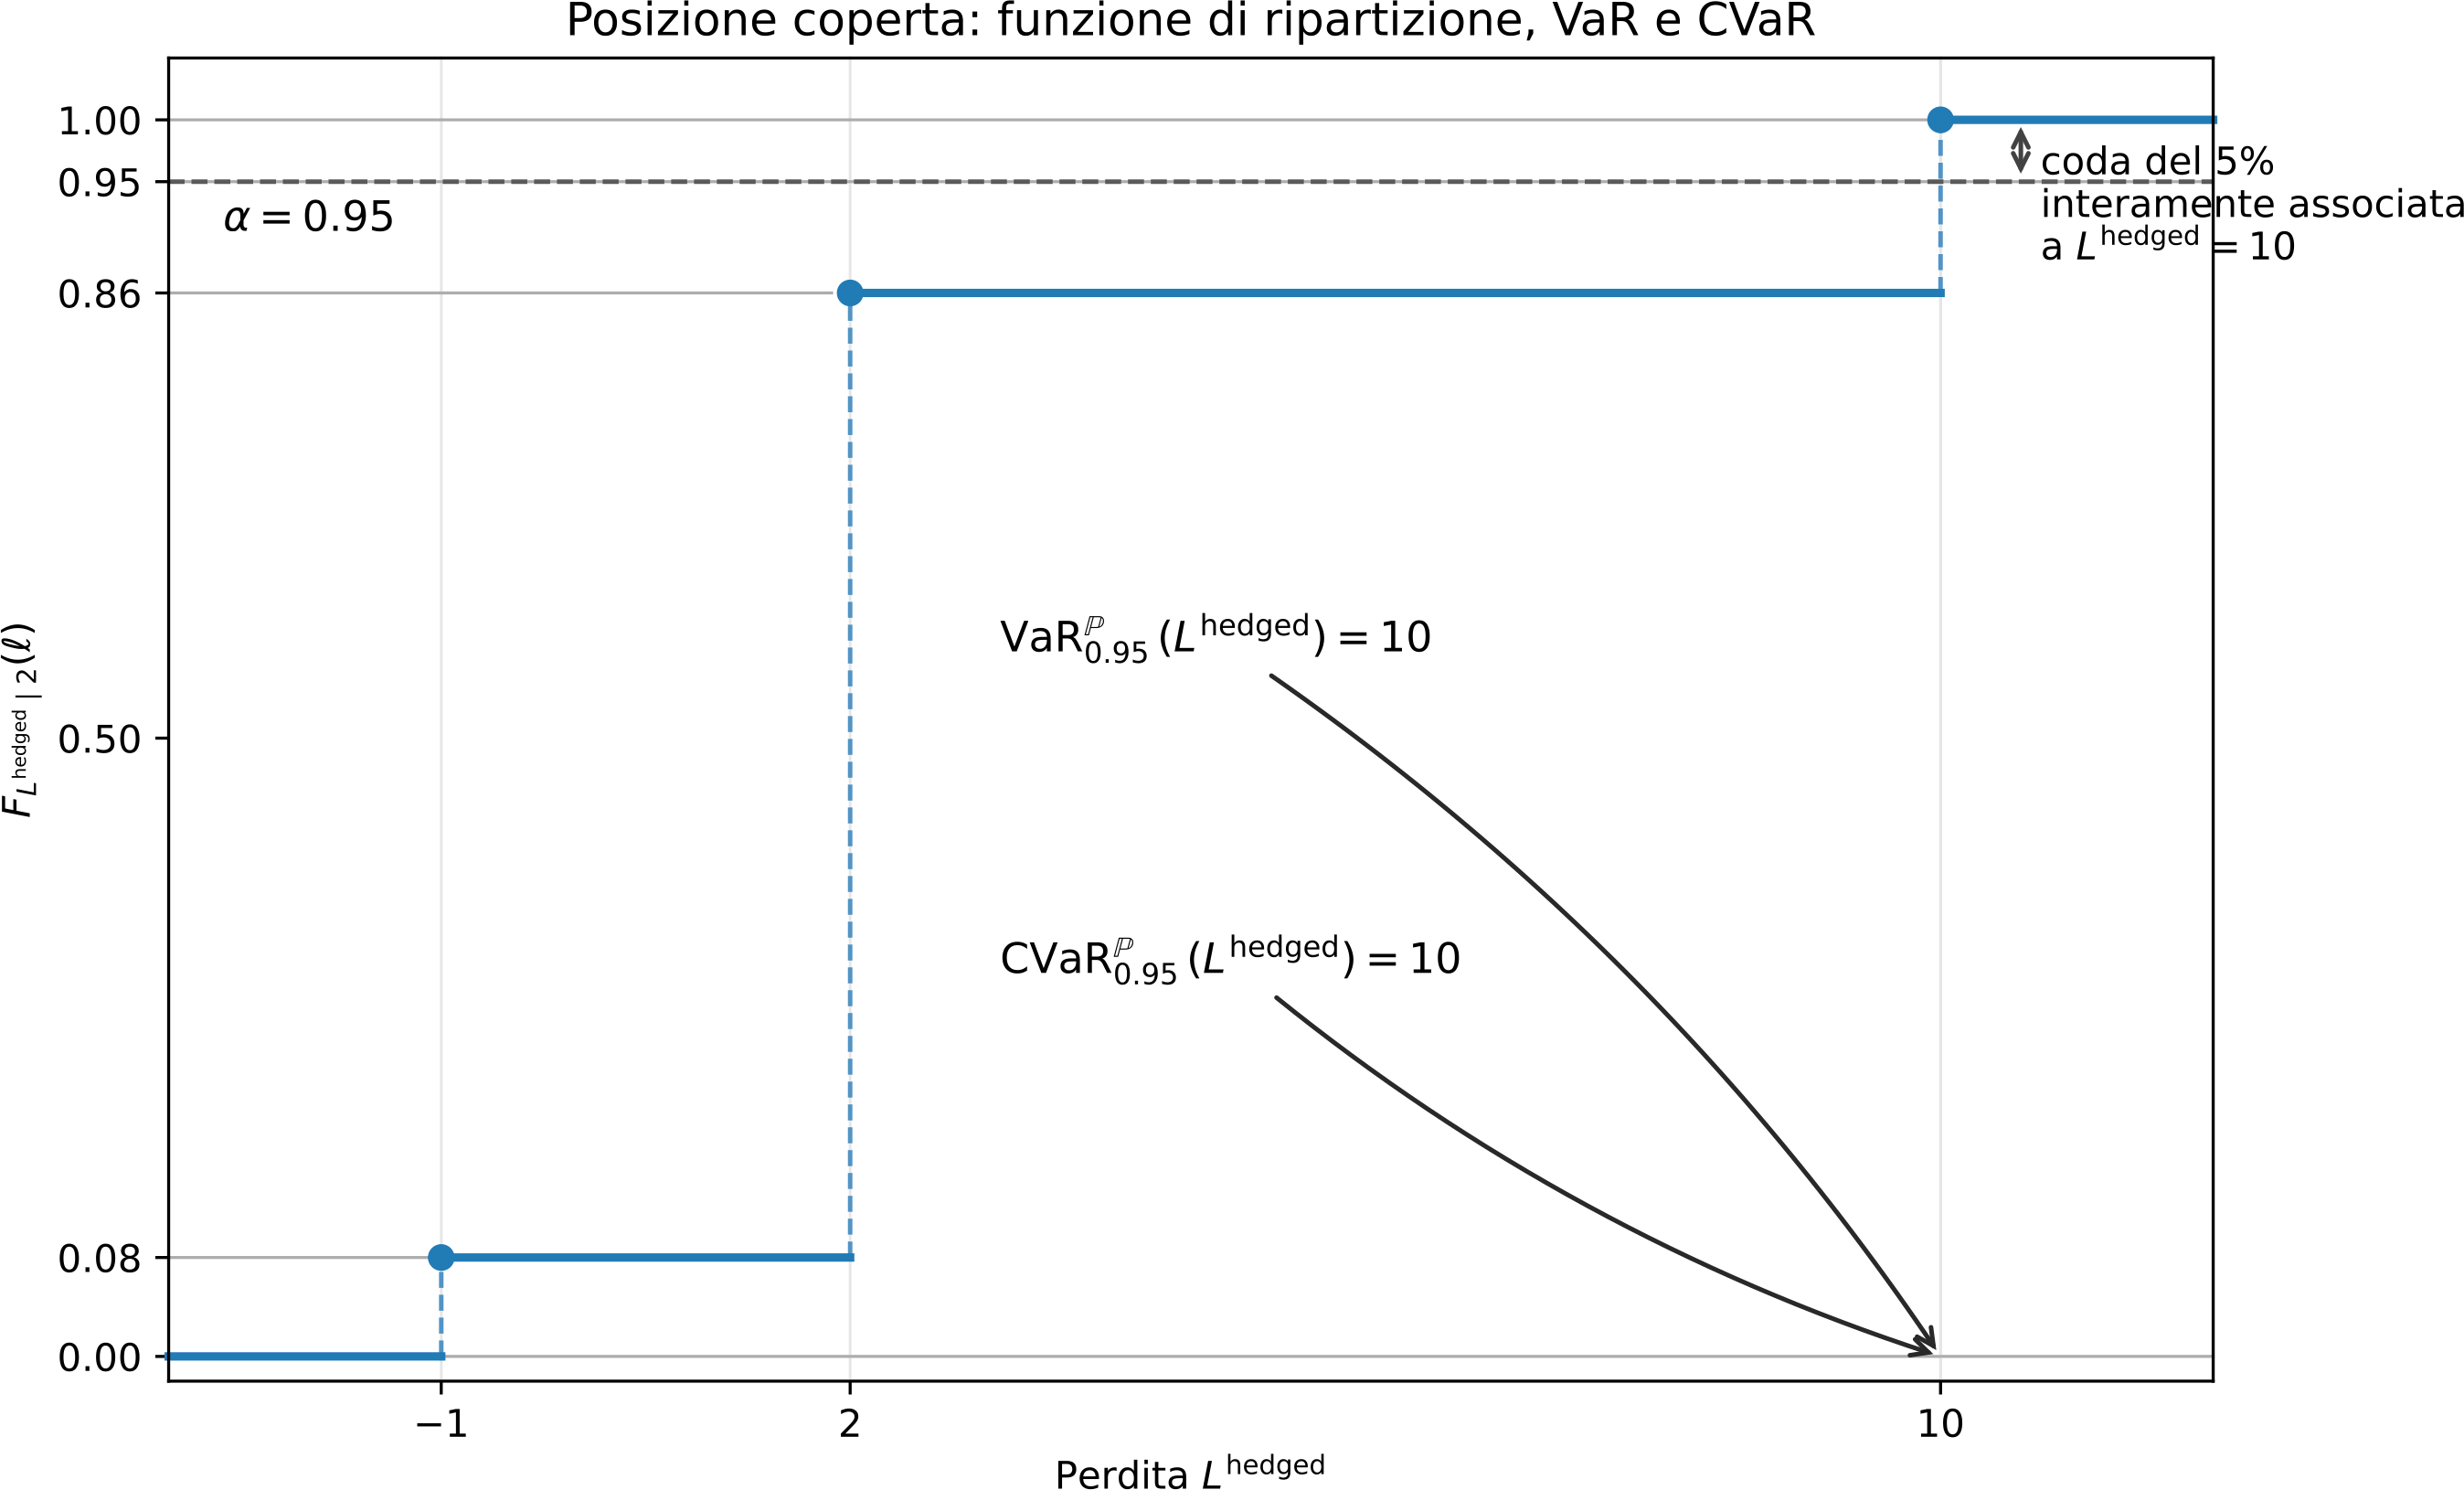
\includegraphics[width=0.82\textwidth]
{../graphics/Cap09_cdf_hedged_var_cvar.png}
\caption{Funzione di ripartizione della perdita della posizione coperta.
Al livello $\alpha=0.95$, si ha $\VaR_{0.95}^{\Prob}(L^{\mathrm{hedged}})=10$.
La coda peggiore di probabilit\`{a} $0.05$ \`{e} interamente contenuta
nell'atomo in corrispondenza della perdita $10$, e quindi
$\CVaR_{0.95}^{\Prob}(L^{\mathrm{hedged}})=10$.}
\label{fig:cap09-cdf-hedged-var-cvar}
\end{figure}


Il confronto complessivo \`{e}

\[
\begin{array}{lcc}
\hline
\text{misura}
&
\text{posizione non coperta}
&
\text{posizione coperta}
\\
\hline
\E^{\Prob}[L]
&
2.68
&
2.88
\\
\VaR_{0.95}^{\Prob}(L)
&
8
&
10
\\
\CVaR_{0.95}^{\Prob}(L)
&
39.2
&
10
\\
\hline
\end{array}
\]

La copertura riduce fortemente il CVaR, poich\'{e} elimina la perdita
estrema da default. Nello stesso esempio, tuttavia, la perdita attesa
aumenta da $2.68$ a $2.88$, poich\'{e}

\[
C^{\mathrm{premi}}
=
2
>
1.80
=
\E^{\Prob}
\left[
\Pi^{\mathrm{CDS}}
\right].
\]

Anche il VaR aumenta, passando da $8$ a $10$. Il premio certo sposta
infatti verso destra le perdite negli stati non-default e porta la
perdita da downgrade da $8$ a $10$.

Non vi \`{e} contraddizione tra questi risultati. Il CDS modifica la
forma dell'intera distribuzione: pu\`{o} ridurre la severit\`{a} della
coda estrema e, contemporaneamente, aumentare la perdita media o un
determinato quantile.

Il costo $2$ non deve essere interpretato come valore atteso fisico
della protezione. Il premio contrattuale viene determinato sotto la
misura risk-neutral, mentre le misure di rischio della posizione
coperta sono calcolate sotto la misura fisica.

\subsection{Limiti della copertura}

\label{subsec:cap9-limiti-copertura-cds}

La riduzione del rischio ottenuta mediante un CDS dipende dalla
corrispondenza tra il contratto di protezione e l'esposizione
sottostante.

\paragraph{Basis risk.}

Il valore dell'esposizione e quello del CDS possono reagire in modo
differente alle variazioni del merito creditizio, della liquidit\`{a}
e delle condizioni di mercato. Il differenziale tra lo spread
dell'obbligazione e lo spread del CDS pu\`{o} quindi variare nel tempo.
La copertura basata sul CDS non replica necessariamente in modo esatto
le variazioni di valore dell'esposizione.

\paragraph{Mismatch di nozionale.}

Se il nozionale del CDS differisce dall'esposizione effettiva, il
pagamento di protezione pu\`{o} essere insufficiente oppure eccedere la
perdita creditizia. Nel primo caso rimane una quota di rischio non
coperta; nel secondo si determina una posizione sovracoperta.

\paragraph{Mismatch di scadenza.}

La scadenza del CDS pu\`{o} essere anteriore o posteriore rispetto a
quella dell'esposizione. Se la protezione termina prima
dell'esposizione, il rischio di default riemerge dopo la scadenza del
CDS. Se la protezione ha durata superiore, possono essere sostenuti
premi relativi a un periodo nel quale l'esposizione non \`{e} pi\`{u}
presente.

\paragraph{Perdite da migrazione.}

Nella formulazione basata sul solo pagamento al credit event, il CDS
non effettua alcun pagamento in seguito a un semplice downgrade. La
perdita mark-to-market dell'obbligazione pu\`{o} quindi rimanere
scoperta.

In una valutazione mark-to-market, il valore del CDS tende a crescere
quando peggiora la qualit\`{a} creditizia della reference entity e
pu\`{o} compensare parzialmente la perdita dell'obbligazione. La
compensazione non \`{e} tuttavia necessariamente completa, a causa del
basis risk, della diversa scadenza e della diversa sensibilit\`{a}
degli strumenti agli spread.

\paragraph{Rischio di controparte.}

La protezione \`{e} efficace soltanto se il protection seller \`{e} in
grado di effettuare il pagamento previsto dal contratto. Il default o
il deterioramento della controparte pu\`{o} ridurre il valore della
copertura proprio negli scenari nei quali la protezione risulta
necessaria.

\paragraph{Evento economico ed evento contrattuale.}

Un grave deterioramento economico dell'emittente non coincide
necessariamente con un credit event riconosciuto dal contratto. Il
pagamento del CDS dipende dalla definizione giuridica e contrattuale
dell'evento creditizio, non dalla sola presenza di una perdita
economica sull'esposizione.

La qualit\`{a} della copertura deve quindi essere valutata confrontando
le distribuzioni complete delle due posizioni:

\[
L^{\mathrm{unhedged}}
\qquad
\text{e}
\qquad
L^{\mathrm{hedged}}.
\]

Una riduzione del CVaR non implica necessariamente una riduzione della
perdita attesa o del VaR. Le differenti misure descrivono aspetti
diversi della distribuzione e possono muoversi in direzioni opposte
quando il pagamento di protezione elimina gli eventi estremi, mentre
il costo dei premi incide su tutti o su molti degli altri stati.

\section{Dal singolo emittente al portafoglio}

\label{sec:cap9-portafoglio}

Le sezioni precedenti hanno considerato il rischio di una singola
esposizione. Un portafoglio creditizio contiene invece numerosi
emittenti, eventualmente caratterizzati da rating iniziali,
esposizioni, recovery rate e matrici di transizione differenti.

Il passaggio dal singolo emittente al portafoglio non consiste nella
sola somma delle probabilit\`{a} marginali. Occorre specificare anche
come le migrazioni dei rating e i default dei differenti emittenti
dipendano tra loro.

Salvo diversa indicazione, in questa sezione le probabilit\`{a} e le
misure di rischio sono considerate sotto la misura fisica $\Prob$.

\subsection{Perdita aggregata}

\label{subsec:cap9-perdita-portafoglio}

Consideriamo un portafoglio formato da $N$ esposizioni. Per
l'esposizione $n$, indichiamo con $X_{n,h}$ il rating alla data $h$ e
con

\[
L_{n,h}
=
\ell_n(X_{n,h},h)
\]

la corrispondente perdita.

La funzione $\ell_n$ pu\`{o} dipendere dalle caratteristiche
specifiche dell'esposizione, tra le quali:

\[
\mathrm{EAD}_{n,h},
\qquad
\mathrm{LGD}_{n,h},
\qquad
\text{scadenza},
\qquad
\text{struttura dei flussi}.
\]

Nel modello default-only, ad esempio,

\[
L_{n,h}
=
\mathrm{EAD}_{n,h}
\mathrm{LGD}_{n,h}
\1_{\{\tau_{D,n}\leq h\}},
\]

dove $\tau_{D,n}$ indica il tempo di default dell'emittente $n$.

Nel modello basato sulle migrazioni del rating, invece,

\[
L_{n,h}
=
V_n^{\mathrm{ref}}(h)
-
V_{n,X_{n,h}}(h),
\]

cosicch\'{e} la perdita pu\`{o} essere generata anche da un downgrade
che non determina il default.

La perdita aggregata del portafoglio all'orizzonte $h$ \`{e}

\[
L_h^{\mathrm{port}}
=
\sum_{n=1}^{N}
L_{n,h}.
\]

Per linearit\`{a} del valore atteso,

\[
\E^{\Prob}
\left[
L_h^{\mathrm{port}}
\right]
=
\sum_{n=1}^{N}
\E^{\Prob}
\left[
L_{n,h}
\right].
\]

Questa relazione vale indipendentemente dalla struttura di dipendenza
tra le esposizioni. Per calcolare la perdita attesa del portafoglio
sono quindi sufficienti le distribuzioni marginali delle singole
perdite.

La varianza della perdita aggregata \`{e} invece

\[
\begin{split}
\Var^{\Prob}
\left(
L_h^{\mathrm{port}}
\right)
&=
\sum_{n=1}^{N}
\Var^{\Prob}(L_{n,h})
\\
&\quad
+
2
\sum_{n=1}^{N-1}
\sum_{m=n+1}^{N}
\Cov^{\Prob}(L_{n,h},L_{m,h}).
\end{split}
\]

Le covarianze mostrano che la dispersione della perdita di portafoglio
dipende dal modo in cui le perdite individuali tendono a verificarsi
congiuntamente.

La dipendenza diventa ancora pi\`{u} importante per il VaR e il CVaR,
che dipendono dalla forma complessiva della distribuzione aggregata e
non possono essere ricavati sommando le corrispondenti misure
marginali.

In generale,

\[
\VaR_{\alpha}^{\Prob}
\left(
\sum_{n=1}^{N}L_{n,h}
\right)
\neq
\sum_{n=1}^{N}
\VaR_{\alpha}^{\Prob}(L_{n,h}),
\]

e analogamente il CVaR del portafoglio deve essere calcolato sulla
distribuzione di $L_h^{\mathrm{port}}$.

\subsection{Distribuzioni marginali e distribuzione congiunta}

\label{subsec:cap9-marginali-congiunta}

Per ciascun emittente $n=1,...,N$, la matrice di transizione
$P_n^{\Prob}$ determina la distribuzione del suo rating futuro. Se
l'emittente parte dal rating $i_n$, si ha

\[
\Prob
\left(
X_{n,h}=j
\mid
X_{n,0}=i_n
\right)
=
\left[
\left(P_n^{\Prob}\right)^h
\right]_{i_nj}.
\]

Queste probabilit\`{a} descrivono il comportamento del singolo
emittente considerato separatamente dagli altri. Esse costituiscono la
distribuzione marginale del rating $X_{n,h}$.

Attraverso la funzione di perdita $\ell_n$, dalla distribuzione del
rating si ricava la distribuzione marginale della perdita individuale

\[
L_{n,h}
=
\ell_n(X_{n,h},h).
\]

Per ciascun emittente $n$, la matrice di transizione
$P_n^{\Prob}$ determina la distribuzione del rating futuro,
condizionatamente al rating iniziale dell'emittente stesso:

\[
\Prob
\left(
X_{n,h}=j
\mid
X_{n,0}=i_n
\right)
=
\left[
\left(P_n^{\Prob}\right)^h
\right]_{i_nj}.
\]

Queste probabilit\`{a} descrivono separatamente i possibili rating
futuri di ciascun emittente. Esse determinano quindi le distribuzioni
individuali delle variabili

\[
X_{1,h},
X_{2,h},
\ldots,
X_{N,h}.
\]

Per rappresentare congiuntamente i rating futuri dell'intero
portafoglio introduciamo il vettore

\[
\mathbf{X}_h
=
\left(
X_{1,h},
X_{2,h},
\ldots,
X_{N,h}
\right),
\]

e il corrispondente vettore dei rating iniziali

\[
\mathbf{X}_0
=
\left(
X_{1,0},
X_{2,0},
\ldots,
X_{N,0}
\right).
\]

Rispetto al vettore $\mathbf{X}_h$, le distribuzioni individuali dei
singoli rating sono dette \emph{distribuzioni marginali}. Esse
indicano le probabilit\`{a} dei possibili rating futuri di ciascun
emittente considerato separatamente, ma non specificano con quali
probabilit\`{a} tali rating si realizzino simultaneamente.

Per descrivere le realizzazioni simultanee occorre invece conoscere la
distribuzione congiunta del vettore $\mathbf{X}_h$. Essa assegna una
probabilit\`{a} a ogni possibile configurazione dei rating futuri:

\[
\begin{split}
&
\Prob
\left(
\mathbf{X}_h=(j_1,\ldots,j_N)
\mid
\mathbf{X}_0=(i_1,\ldots,i_N)
\right)
\\
&=
\Prob
\left(
X_{1,h}=j_1,
\ldots,
X_{N,h}=j_N
\mid
X_{1,0}=i_1,
\ldots,
X_{N,0}=i_N
\right).
\end{split}
\]

La distribuzione congiunta \`{e} necessaria per determinare la
distribuzione della perdita aggregata

\[
L_h^{\mathrm{port}}
=
\sum_{n=1}^{N}
\ell_n(X_{n,h},h).
\]

Le matrici di transizione dei singoli emittenti determinano dunque le
distribuzioni marginali dei rating e delle corrispondenti perdite, ma
non determinano la distribuzione congiunta delle loro realizzazioni e,
di conseguenza, non sono sufficienti per ricavare la distribuzione
della perdita di portafoglio.

La relazione fondamentale \`{e}

\[
\boxed{
\begin{array}{c}
\text{matrici di transizione dei singoli emittenti}
\\[1mm]
\downarrow
\\[1mm]
\text{distribuzioni individuali dei rating}
\\
\text{e delle corrispondenti perdite}
\\[3mm]
\not\Longrightarrow
\\[3mm]
\text{distribuzione della perdita aggregata}
\end{array}
}
\]


Soltanto assumendo indipendenza tra le migrazioni si potrebbe scrivere

\[
\begin{split}
&
\Prob
\left(
X_{1,h}=j_1,\ldots,X_{N,h}=j_N
\mid
\mathbf{X}_0=\mathbf{i}
\right)
\\
&=
\prod_{n=1}^{N}
\Prob
\left(
X_{n,h}=j_n
\mid
X_{n,0}=i_n
\right).
\end{split}
\]

L'indipendenza costituisce tuttavia un'ipotesi particolarmente forte, e nella pratica poco realistica.
Durante una recessione, una crisi settoriale o uno shock finanziario,
pi\`{u} emittenti possono subire simultaneamente downgrade o default.

\begin{example}

Consideriamo un portafoglio formato da due emittenti. Il vettore dei
rating iniziali \`{e}

\[
\mathbf{X}_0
=
\left(
X_{1,0},
X_{2,0}
\right).
\]

Supponiamo che entrambi gli emittenti appartengano inizialmente alla
classe di rating $2$:

\[
\mathbf{X}_0
=
\mathbf{i}
=
(2,2).
\]

All'orizzonte $h$, ciascun emittente pu\`{o} soltanto permanere nello
stato $2$ oppure entrare nello stato di default $D$:

\[
X_{1,h},X_{2,h}
\in
\{2,D\}.
\]

Il vettore dei rating futuri \`{e}

\[
\mathbf{X}_h
=
\left(
X_{1,h},
X_{2,h}
\right).
\]

Le sue possibili realizzazioni sono

\[
\mathbf{j}
\in
\{
(2,2),
(D,2),
(2,D),
(D,D)
\}.
\]

Per la configurazione iniziale fissata $\mathbf{i}=(2,2)$, indichiamo
con

\[
p_h(\mathbf{i},\mathbf{j})
=
\Prob
\left(
\mathbf{X}_h=\mathbf{j}
\mid
\mathbf{X}_0=\mathbf{i}
\right)
\]

la probabilit\`{a} della configurazione futura $\mathbf{j}$.

Al variare di $\mathbf{j}$, le quantit\`{a}
$p_h(\mathbf{i},\mathbf{j})$ costituiscono la distribuzione congiunta
dei rating futuri, condizionata alla configurazione iniziale
$\mathbf{i}$.

Supponiamo che entrambi gli emittenti abbiano probabilit\`{a}
individuale di default pari a $0.05$:

\[
\Prob
\left(
X_{1,h}=D
\mid
\mathbf{X}_0=\mathbf{i}
\right)
=
\Prob
\left(
X_{2,h}=D
\mid
\mathbf{X}_0=\mathbf{i}
\right)
=
0.05.
\]

Le corrispondenti probabilit\`{a} di permanenza nello stato $2$ sono
pari a $0.95$. Confronteremo due diverse distribuzioni congiunte,
entrambe compatibili con queste stesse distribuzioni marginali.

\paragraph{Primo modello: default indipendenti.}

Se i rating futuri dei due emittenti sono indipendenti,
condizionatamente alla configurazione iniziale, la distribuzione
congiunta \`{e}

\[
\begin{array}{c|cc|c}
&
X_{2,h}=2
&
X_{2,h}=D
&
\text{totale}
\\
\hline
X_{1,h}=2
&
0.9025
&
0.0475
&
0.95
\\
X_{1,h}=D
&
0.0475
&
0.0025
&
0.05
\\
\hline
\text{totale}
&
0.95
&
0.05
&
1
\end{array}
\]

Le somme di riga forniscono la distribuzione marginale di $X_{1,h}$,
mentre le somme di colonna forniscono la distribuzione marginale di
$X_{2,h}$.

In particolare,

\[
\Prob
\left(
X_{1,h}=D
\mid
\mathbf{X}_0=\mathbf{i}
\right)
=
0.0475+0.0025
=
0.05,
\]

e

\[
\Prob
\left(
X_{2,h}=D
\mid
\mathbf{X}_0=\mathbf{i}
\right)
=
0.0475+0.0025
=
0.05.
\]

La probabilit\`{a} congiunta del doppio default \`{e}

\[
\Prob
\left(
X_{1,h}=D,
X_{2,h}=D
\mid
\mathbf{X}_0=\mathbf{i}
\right)
=
0.0025.
\]

\paragraph{Secondo modello: default perfettamente dipendenti.}

Supponiamo ora che i due emittenti subiscano sempre il default
congiuntamente. La distribuzione congiunta diventa

\[
\begin{array}{c|cc|c}
&
X_{2,h}=2
&
X_{2,h}=D
&
\text{totale}
\\
\hline
X_{1,h}=2
&
0.95
&
0
&
0.95
\\
X_{1,h}=D
&
0
&
0.05
&
0.05
\\
\hline
\text{totale}
&
0.95
&
0.05
&
1
\end{array}
\]

Le probabilit\`{a} marginali sono rimaste invariate:

\[
\Prob
\left(
X_{1,h}=D
\mid
\mathbf{X}_0=\mathbf{i}
\right)
=
0.05,
\]

e

\[
\Prob
\left(
X_{2,h}=D
\mid
\mathbf{X}_0=\mathbf{i}
\right)
=
0.05.
\]

La probabilit\`{a} congiunta del doppio default \`{e} invece

\[
\Prob
\left(
X_{1,h}=D,
X_{2,h}=D
\mid
\mathbf{X}_0=\mathbf{i}
\right)
=
0.05.
\]

Le due distribuzioni congiunte hanno pertanto gli stessi margini, ma
attribuiscono probabilit\`{a} differenti alle realizzazioni
simultanee:

\[
\begin{array}{c|cc}
&
\text{indipendenza}
&
\text{dipendenza perfetta}
\\
\hline
\Prob
\left(
X_{1,h}=D,
X_{2,h}=D
\mid
\mathbf{X}_0=\mathbf{i}
\right)
&
0.0025
&
0.05
\end{array}
\]

Supponiamo infine che ciascuna esposizione produca una perdita unitaria
in caso di default:

\[
L_{1,h}
=
\1_{\{X_{1,h}=D\}},
\qquad
L_{2,h}
=
\1_{\{X_{2,h}=D\}}.
\]

La perdita aggregata \`{e}

\[
L_h^{\mathrm{port}}
=
L_{1,h}+L_{2,h}.
\]

La corrispondenza tra configurazioni dei rating e perdita aggregata
\`{e}

\[
\begin{array}{c|cccc}
\mathbf{X}_h
&
(2,2)
&
(D,2)
&
(2,D)
&
(D,D)
\\
\hline
L_h^{\mathrm{port}}
&
0
&
1
&
1
&
2
\end{array}
\]

Nel modello con default indipendenti si ottiene

\[
\begin{array}{c|ccc}
L_h^{\mathrm{port}}
&
0
&
1
&
2
\\
\hline
\Prob
\left(
L_h^{\mathrm{port}}=\ell
\mid
\mathbf{X}_0=\mathbf{i}
\right)
&
0.9025
&
0.0950
&
0.0025
\end{array}
\]

Nel modello con default perfettamente dipendenti si ottiene invece

\[
\begin{array}{c|ccc}
L_h^{\mathrm{port}}
&
0
&
1
&
2
\\
\hline
\Prob
\left(
L_h^{\mathrm{port}}=\ell
\mid
\mathbf{X}_0=\mathbf{i}
\right)
&
0.95
&
0
&
0.05
\end{array}
\]

Le distribuzioni marginali dei rating individuali sono identiche nei
due modelli. La diversa struttura di dipendenza modifica tuttavia la
distribuzione congiunta dei rating e, di conseguenza, la distribuzione
della perdita aggregata.

\end{example}

\subsection{Concentrazione e fattori comuni}

\label{subsec:cap9-concentrazione-fattori}

La dipendenza tra le perdite pu\`{o} derivare da fattori economici
comuni e dalla composizione del portafoglio.

\paragraph{Concentrazione per debitore.}

Un portafoglio \`{e} concentrato per debitore quando una parte
rilevante dell'esposizione complessiva dipende da pochi emittenti. Se

\[
w_n
=
\frac{
\mathrm{EAD}_{n,h}
}{
\displaystyle
\sum_{m=1}^{N}
\mathrm{EAD}_{m,h}
},
\]

un valore elevato di $w_n$ indica che il deterioramento del debitore
$n$ pu\`{o} produrre una quota rilevante della perdita totale.

La presenza di molti emittenti non garantisce quindi
automaticamente una diversificazione effettiva, se il portafoglio
rimane dominato da poche esposizioni di grandi dimensioni.

\paragraph{Concentrazione settoriale.}

Emittenti appartenenti allo stesso settore possono reagire in modo
simile a variazioni dei prezzi delle materie prime, dei tassi di
interesse, della domanda o della regolamentazione.

Un portafoglio composto da numerosi debitori dello stesso settore pu\`{o}
essere poco diversificato, anche quando nessuna singola esposizione
risulta dominante.

\paragraph{Concentrazione geografica.}

La localizzazione degli emittenti in una stessa area economica espone
il portafoglio a shock comuni relativi alla crescita, alla politica
fiscale, al sistema bancario, al rischio sovrano o al quadro
istituzionale.

La diversificazione per numero di debitori pu\`{o} quindi essere
inefficace se le esposizioni rimangono concentrate nella stessa
economia.

\paragraph{Dipendenza macroeconomica.}

Le probabilit\`{a} di transizione possono dipendere da un fattore
macroeconomico comune $Z_h$, ad esempio uno stato di espansione,
rallentamento o recessione.

Condizionatamente a $Z_h$, le transizioni individuali possono essere
modellate come indipendenti:

\[
\begin{split}
&
\Prob
\left(
X_{1,h}=j_1,\ldots,X_{N,h}=j_N
\mid
Z_h,\mathbf{X}_0
\right)
\\
&=
\prod_{n=1}^{N}
\Prob
\left(
X_{n,h}=j_n
\mid
Z_h,X_{n,0}
\right).
\end{split}
\]

Senza condizionare sul fattore comune, le migrazioni risultano invece
dipendenti. Uno stato macroeconomico sfavorevole aumenta
simultaneamente la probabilit\`{a} di downgrade e default di numerosi
emittenti.

\paragraph{Default clustering.}

Con l'espressione \emph{default clustering} si indica la tendenza dei
default a concentrarsi negli stessi periodi anzich\'{e} distribuirsi
uniformemente nel tempo.

Il fenomeno pu\`{o} derivare da recessioni, crisi di liquidit\`{a},
shock settoriali, legami commerciali o esposizioni comuni alle stesse
fonti di finanziamento.

Il clustering aumenta la probabilit\`{a} di perdite aggregate molto
elevate e incide soprattutto sulla parte estrema della distribuzione.
Per questo motivo, trascurare la dipendenza pu\`{o} produrre una
sottostima significativa del VaR e del CVaR di portafoglio.

\subsection{Derivati multi-name}

\label{subsec:cap9-derivati-multiname}

Il CDS analizzato nelle sezioni precedenti \`{e} riferito a una singola
reference entity. Esistono anche derivati di credito il cui payoff
dipende da pi\`{u} emittenti.

Tra i principali strumenti multi-name rientrano:

\begin{itemize}

\item i \emph{CDS index}, riferiti a un insieme standardizzato di
emittenti;

\item i \emph{basket CDS}, riferiti a un paniere di debitori
specificamente selezionato;

\item i contratti \emph{first-to-default}, nei quali la protezione
viene attivata dal primo default all'interno del paniere;

\item le tranche creditizie, il cui payoff dipende dalla perdita
aggregata del portafoglio compresa tra determinati livelli di
assorbimento.

\end{itemize}

Nel contratto first-to-default, il tempo rilevante \`{e}

\[
\tau_{(1)}
=
\min
\{
\tau_{D,1},
\ldots,
\tau_{D,N}
\}.
\]

La probabilit\`{a} che il contratto venga attivato entro l'orizzonte
$H$ \`{e}

\[
\Prob(\tau_{(1)}\leq H).
\]

Questa probabilit\`{a} non pu\`{o} essere determinata conoscendo
soltanto le probabilit\`{a} marginali

\[
\Prob(\tau_{D,n}\leq H).
\]

Occorre specificare la dipendenza tra i tempi di default.

\begin{definition}
Una \emph{tranche creditizia} \`{e} una porzione contrattualmente
definita della perdita aggregata di un portafoglio. Essa \`{e}
identificata da due livelli

\[
0\leq A<B,
\]

dove $A$ \`{e} l'\emph{attachment point} e $B$ il
\emph{detachment point}.
\end{definition}

Indicando con $L_h^{\mathrm{port}}$ la perdita aggregata del
portafoglio, la perdita assorbita dalla tranche pu\`{o} essere
rappresentata come

\[
L_h^{\mathrm{tr}}(A,B)
=
\left(
L_h^{\mathrm{port}}-A
\right)^{+}
-
\left(
L_h^{\mathrm{port}}-B
\right)^{+}.
\]

Equivalentemente,

\[
L_h^{\mathrm{tr}}(A,B)
=
\min
\left\{
\left(
L_h^{\mathrm{port}}-A
\right)^{+},
B-A
\right\}.
\]Indicando con $L_h^{\mathrm{port}}$ la perdita aggregata del
portafoglio, la perdita assorbita dalla tranche pu\`{o} essere
rappresentata come

\[
L_h^{\mathrm{tr}}(A,B)
=
\left(
L_h^{\mathrm{port}}-A
\right)^{+}
-
\left(
L_h^{\mathrm{port}}-B
\right)^{+}.
\]

Equivalentemente,

\[
L_h^{\mathrm{tr}}(A,B)
=
\min
\left\{
\left(
L_h^{\mathrm{port}}-A
\right)^{+},
B-A
\right\}.
\]

La Figura~\ref{fig:cap09-tranche-creditizia} mostra come la perdita
della tranche dipenda dalla perdita aggregata del portafoglio.

\begin{figure}[htbp]
\centering
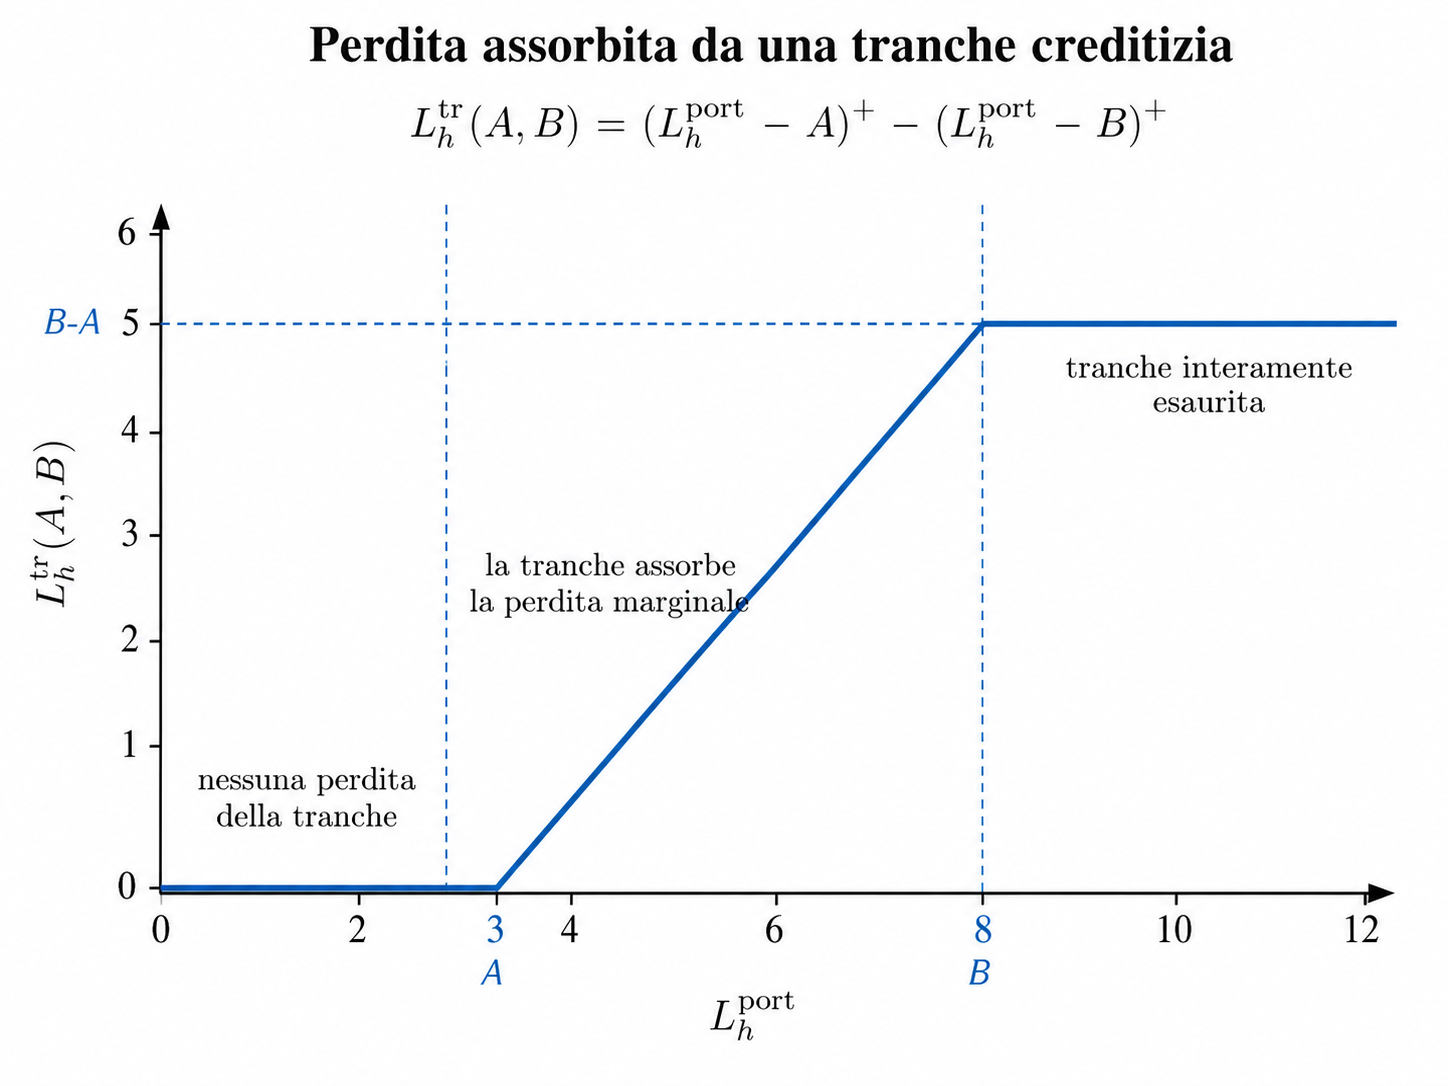
\includegraphics[width=0.82\textwidth]
{../graphics/Cap09_tranche_creditizia.png}
\caption{Profilo della perdita assorbita da una tranche creditizia con
attachment point $A$ e detachment point $B$.}
\label{fig:cap09-tranche-creditizia}
\end{figure}

La tranche non subisce perdite finch\'{e}

\[
L_h^{\mathrm{port}}\leq A.
\]

Per

\[
A<L_h^{\mathrm{port}}<B,
\]

la perdita della tranche cresce nella stessa misura della perdita
aggregata eccedente l'attachment point. Infine, quando

\[
L_h^{\mathrm{port}}\geq B,
\]

la tranche risulta interamente esaurita e la sua perdita raggiunge il
valore massimo

\[
B-A.
\]



La tranche non subisce perdite finch\'{e} la perdita aggregata rimane
inferiore ad $A$. Assorbe le perdite comprese tra $A$ e $B$ ed
\`{e} interamente esaurita quando

\[
L_h^{\mathrm{port}}\geq B.
\]

Per descrivere i flussi associati alla tranche occorre quindi
conoscere la distribuzione della perdita aggregata del portafoglio.
La dipendenza tra i default, influenzando la frequenza e la
concentrazione delle perdite elevate, diventa pertanto un elemento
essenziale.

Il pricing dei derivati multi-name non viene sviluppato nel presente
corso. Questi strumenti mostrano tuttavia perch\'{e} la modellizzazione
della dipendenza sia indispensabile: lo stesso insieme di probabilit\`{a}
marginali pu\`{o} generare valori e distribuzioni di perdita molto
differenti al variare della struttura congiunta.

\subsection{Raccordo con la Lezione 10}

\label{subsec:cap9-raccordo-lezione10}

Per un portafoglio con molti emittenti, la costruzione analitica della
distribuzione congiunta pu\`{o} diventare rapidamente complessa. La
Lezione~10 utilizzer\`{a} la simulazione per generare scenari congiunti
dei rating e delle perdite.

La struttura dell'applicazione sar\`{a}

\[
\boxed{
\begin{array}{c}
\text{transizioni individuali}
\\
+
\\
\text{dipendenza e fattori comuni}
\\
+
\\
\mathrm{LGD}\text{ ed }\mathrm{EAD}
\\
\downarrow
\\
\text{distribuzione simulata della perdita di portafoglio}.
\end{array}
}
\]

In ciascuno scenario simulato si proceder\`{a} a:

\begin{enumerate}

\item generare lo stato del fattore macroeconomico comune;

\item simulare le transizioni dei singoli emittenti condizionatamente
al fattore comune e ai rating iniziali;

\item associare a ogni stato futuro una perdita dipendente da
$\mathrm{LGD}$, $\mathrm{EAD}$ e dalla variazione di valore
dell'esposizione;

\item aggregare le perdite individuali:

\[
L_h^{\mathrm{port}}
=
\sum_{n=1}^{N}L_{n,h};
\]

\item ripetere la simulazione per ottenere una distribuzione empirica
della perdita aggregata;

\item stimare perdita attesa, varianza, VaR e CVaR del portafoglio.

\end{enumerate}

La Lezione~10 mostrer\`{a} quindi il passaggio operativo dalle matrici
marginali di transizione a una distribuzione di portafoglio nella quale
la dipendenza viene specificata e simulata esplicitamente.

\section{Impiego gestionale e regolamentare delle misure}

\label{sec:cap9-impiego-gestionale-regolamentare}

Le misure introdotte nel capitolo trovano applicazione nella gestione
del rischio, nella redazione del bilancio e nella valutazione
dell'adeguatezza patrimoniale. I diversi ambiti utilizzano concetti
collegati, ma non coincidenti.

In particolare, occorre distinguere tra:

\begin{itemize}
\item la perdita attesa;
\item gli accantonamenti contabili;
\item il capitale economico;
\item i requisiti patrimoniali prudenziali.
\end{itemize}

La presente sezione fornisce soltanto un inquadramento professionale.
La disciplina contabile e prudenziale completa viene rinviata agli
insegnamenti specialistici.

\subsection{Accantonamenti e IFRS 9}

\label{subsec:cap9-ifrs9}

Il principio contabile IFRS~9 adotta un modello fondato sulle
\emph{expected credit losses}, indicate con ECL. L'accantonamento
contabile dipende dall'evoluzione del rischio creditizio dello
strumento rispetto alla data della sua rilevazione iniziale.

L'IFRS~9 distingue due basi di misurazione delle perdite attese:

\begin{itemize}

\item l'\emph{expected credit loss a 12 mesi};

\item la \emph{lifetime expected credit loss}.

\end{itemize}

La differenza riguarda l'orizzonte entro il quale pu\`{o} verificarsi
il default. L'ECL a 12 mesi considera le perdite lungo la vita residua
dello strumento generate da eventi di default possibili nei dodici
mesi successivi. La lifetime ECL considera invece le perdite generate
da tutti i default possibili durante l'intera vita residua.

Quando si verifica un incremento significativo del rischio creditizio,
l'accantonamento viene invece determinato sulla base della
\emph{lifetime expected credit loss}, che considera gli eventi di
default possibili lungo l'intera vita residua dello strumento.

In forma schematica,

\[
\begin{array}{ccl}
\text{assenza di incremento significativo}
&
\longrightarrow
&
\text{ECL a 12 mesi},
\\[2mm]
\text{incremento significativo del rischio}
&
\longrightarrow
&
\text{lifetime ECL}.
\end{array}
\]

La valutazione dell'incremento significativo del rischio creditizio
richiede il confronto tra il rischio di default alla data corrente e
quello esistente al momento della rilevazione iniziale. Non coincide
quindi con la sola osservazione del rating corrente o con il
verificarsi del default.

Il modello markoviano sviluppato nel capitolo consente di rappresentare
in modo semplificato il collegamento tra transizioni dei rating e
lifetime ECL. Utilizzando una matrice di transizione predittiva
$P^{\Prob}$, le probabilit\`{a} marginali di default sono

\[
\mathrm{PD}_{i}^{\mathrm{marg}}(h)
=
\left[
\left(P^{\Prob}\right)^h
\right]_{iD}
-
\left[
\left(P^{\Prob}\right)^{h-1}
\right]_{iD}.
\]

In un modello discreto semplificato, definiamo la perdita creditizia
attualizzata lungo la vita residua come

\[
L_i^{\mathrm{life}}
=
\sum_{h=1}^{H}
d_h
\mathrm{LGD}_h
\mathrm{EAD}_h
\1_{\{\tau_D=h\}}.
\]

Se il default avviene alla data $h$, soltanto l'indicatrice
$\1_{\{\tau_D=h\}}$ assume valore uno. Se invece $\tau_D>H$, tutte le
indicatrici sono nulle e la perdita da default \`{e} pari a zero.
La lifetime expected credit loss \`{e} quindi il valore atteso della
perdita lungo la vita residua:

\[
\begin{split}
\mathrm{ECL}_{i}^{\mathrm{life}}
&=
\E^{\Prob}
\left[
L_i^{\mathrm{life}}
\mid X_0=i
\right]
\\
&=
\sum_{h=1}^{H}
d_h
\mathrm{PD}_{i}^{\mathrm{marg}}(h)
\mathrm{LGD}_h
\mathrm{EAD}_h.
\end{split}
\]
Il collegamento concettuale \`{e} quindi

\[
\boxed{
\left(P^{\Prob}\right)^h
\longrightarrow
\text{term structure delle probabilit\`{a} di default}
\longrightarrow
\text{lifetime ECL}.
}
\]

Nel modello annuale semplificato, l'ECL a 12 mesi utilizza la
probabilit\`{a} degli eventi di default che possono verificarsi nel
primo anno:

\[
\mathrm{ECL}_{i}^{12\mathrm{m}}
=
d_1
\mathrm{PD}_{i}^{\mathrm{marg}}(1)
\mathrm{LGD}_1
\mathrm{EAD}_1.
\]

Le formule precedenti costituiscono una rappresentazione didattica:
l'IFRS~9 non prescrive l'impiego di una matrice di transizione.

Nel modello qui adottato, la matrice $P^{\Prob}$ viene utilizzata per
ottenere probabilit\`{a} di default predittive. Una matrice stimata
sulle transizioni storiche pu\`{o} costituire il punto di partenza, ma
le probabilit\`{a} utilizzate nel calcolo dell'ECL devono riflettere
anche le condizioni correnti e le previsioni ragionevoli
sull'evoluzione futura dell'economia.

Si tratta pertanto di probabilit\`{a} sotto la misura fisica, finalizzate
alla previsione delle perdite, e non di probabilit\`{a} risk-neutral
utilizzate per il pricing.

\subsection{Capitale economico e capitale prudenziale}

\label{subsec:cap9-capitale-economico-prudenziale}

La perdita attesa, l'accantonamento contabile, il capitale economico
e il requisito patrimoniale prudenziale sono concetti collegati, ma
rispondono a finalit\`{a} differenti.

La \emph{perdita attesa} (\emph{Expected Loss}, \emph{EL}) \`{e} il
valore medio della variabile casuale perdita sotto la distribuzione
predittiva adottata:

\[
\mathrm{EL}
=
\E^{\Prob}[L].
\]

Essa rappresenta la perdita media associata all'esposizione o al
portafoglio nel modello considerato.

L'\emph{accantonamento contabile per perdite}
(\emph{loss allowance}) \`{e} invece l'importo rilevato in bilancio
a fronte delle perdite creditizie attese. Nell'IFRS~9 esso viene
misurato mediante le \emph{Expected Credit Losses} (\emph{ECL}),
utilizzando, a seconda dell'evoluzione del rischio creditizio, l'ECL
a 12 mesi oppure la lifetime ECL.

L'accantonamento contabile \`{e} quindi collegato alla perdita attesa,
ma non coincide necessariamente con la quantit\`{a} $\mathrm{EL}$
calcolata mediante un generico modello interno. La sua determinazione
dipende dalle regole contabili applicabili, dall'orizzonte considerato,
dall'attualizzazione e dalle informazioni previsionali utilizzate.

Il \emph{capitale economico} (\emph{Economic Capital}, \emph{EC})
\`{e} una misura gestionale interna delle risorse destinate ad
assorbire le perdite superiori alla perdita attesa, entro un
determinato orizzonte e livello di confidenza $\alpha$.

Secondo la convenzione adottata nel capitolo,

\[
\mathrm{EC}_{\alpha}
=
\VaR_{\alpha}(L)
-
\mathrm{EL},
\]

dove il \emph{Value at Risk} (\emph{VaR}) rappresenta il quantile
della perdita totale al livello di confidenza $\alpha$.

Il \emph{requisito patrimoniale prudenziale}
(\emph{prudential capital requirement}) \`{e} invece il capitale
richiesto dalle regole di vigilanza. Esso dipende, tra gli altri
elementi, dalle esposizioni, dalle ponderazioni per il rischio, dai
parametri regolamentari, dal metodo di calcolo applicato e dagli
eventuali requisiti o riserve aggiuntivi previsti dal quadro
prudenziale.

Le quattro nozioni possono essere sintetizzate come segue:

\[
\begin{array}{p{4.2cm}p{7.4cm}}
\hline
\textbf{Concetto}
&
\textbf{Funzione principale}
\\
\hline
\emph{Expected Loss} (\emph{EL})
&
misurare la perdita media prodotta dal modello probabilistico;
\\
\emph{loss allowance}
&
rilevare in bilancio le perdite creditizie attese misurate mediante
le \emph{ECL};
\\
\emph{Economic Capital} (\emph{EC})
&
determinare internamente le risorse destinate ad assorbire le perdite
superiori alla perdita attesa;
\\
\emph{prudential capital requirement}
&
determinare il capitale richiesto dalle regole di vigilanza.
\\
\hline
\end{array}
\]

La relazione

\[
\mathrm{EC}_{\alpha}
=
\VaR_{\alpha}(L)
-
\mathrm{EL}
\]

costituisce pertanto una convenzione gestionale per il calcolo del
capitale economico. Non rappresenta una formula generale per la
determinazione del requisito patrimoniale prudenziale.

\subsection{Stress testing}

\label{subsec:cap9-stress-testing}

Il VaR e il CVaR sono misure probabilistiche ricavate da una
distribuzione stimata delle perdite:

\[
F_L
\longrightarrow
\VaR_{\alpha}(L),
\qquad
\CVaR_{\alpha}(L).
\]

I risultati dipendono quindi dal modello adottato, dai dati utilizzati,
dalla struttura di dipendenza e dalle ipotesi formulate sulle
transizioni, sulle esposizioni e sui tassi di recupero.

Lo stress testing segue una logica differente. Si specifica uno
scenario avverso, ad esempio una recessione, un aumento dei default,
una riduzione dei recovery rate o un deterioramento simultaneo di
determinati settori, e si valuta la perdita che ne deriverebbe.

Indicando con $z^{\mathrm{stress}}$ lo scenario avverso assegnato, si
considera una quantit\`{a} del tipo

\[
L^{\mathrm{stress}}
=
L\left(z^{\mathrm{stress}}\right).
\]

Lo scenario di stress non deve necessariamente essere identificato
con un quantile della distribuzione stimata, n\'{e} deve essergli
attribuita una probabilit\`{a} precisa. La sua funzione \`{e} valutare
la vulnerabilit\`{a} della posizione o del portafoglio rispetto a una
configurazione avversa specifica.

Le due prospettive sono complementari:

\[
\boxed{
\begin{array}{c}
\text{misure probabilistiche}
\quad+\quad
\text{scenari di stress}
\\[-0.5mm]
\longrightarrow
\quad
\text{valutazione pi\`{u} completa del rischio}
\end{array}
}
\]

Il VaR e il CVaR sintetizzano la distribuzione prodotta dal modello; lo
stress testing verifica invece le conseguenze di scenari avversi che
possono risultare particolarmente rilevanti dal punto di vista
gestionale o prudenziale.

\section{Limiti del modello e rischio di modello}

\label{sec:cap9-limiti-rischio-modello}

Le misure di rischio ottenute nel capitolo non sono quantit\`{a}
direttamente osservabili. Esse sono il risultato di una successione di
scelte modellistiche che riguardano la dinamica dei rating, la
traduzione degli stati futuri in perdite e, nel caso di un portafoglio,
la dipendenza tra gli emittenti.

Nel presente capitolo, con \emph{rischio di modello}
(\emph{model risk}) si indica il rischio che una rappresentazione
incompleta, non adeguatamente specificata o non correttamente calibrata
produca stime delle perdite e delle misure di rischio non sufficientemente
affidabili.

I limiti del modello vengono quindi organizzati secondo le principali
componenti della catena di misurazione.

\subsection{Modello delle transizioni}

\label{subsec:cap9-limiti-transizioni}

Il modello delle transizioni determina le probabilit\`{a} associate ai
rating futuri e al default. Le sue conclusioni dipendono dalla validit\`{a}
della struttura markoviana e dalla capacit\`{a} della matrice di
transizione di rappresentare l'evoluzione futura del rischio creditizio.

\paragraph{Validit\`{a} della propriet\`{a} di Markov.}

La propriet\`{a} di Markov assume che, condizionatamente al rating
corrente, la distribuzione del rating futuro non dipenda ulteriormente
dalla storia precedente dell'emittente.

Questa ipotesi pu\`{o} risultare restrittiva. Due emittenti collocati
nella stessa classe di rating possono avere prospettive differenti se
uno vi permane da diversi anni, mentre l'altro vi \`{e} appena entrato
in seguito a un downgrade. La durata della permanenza nello stato, la
direzione delle precedenti migrazioni e altre informazioni storiche
possono quindi contenere capacit\`{a} predittiva non rappresentata dal
solo rating corrente.

In questi casi, il modello pu\`{o} essere ampliato introducendo ulteriori
variabili di stato oppure adottando una dinamica non strettamente
markoviana.

\paragraph{Omogeneit\`{a} temporale.}

Nel modello omogeneo, una sola matrice $P$ descrive le probabilit\`{a}
di transizione in ogni periodo. La distribuzione a $h$ periodi viene
pertanto ottenuta mediante

\[
P^h.
\]

Questa rappresentazione presuppone che le probabilit\`{a} di upgrade,
downgrade e default restino costanti nel tempo. Tale ipotesi pu\`{o}
essere poco realistica quando il rischio creditizio varia con il ciclo
economico, con le condizioni finanziarie o con eventi settoriali.

Se la matrice dipende dal tempo, la probabilit\`{a} di transizione tra
le date $t$ e $t+h$ non \`{e} descritta da $P^h$, ma dal prodotto

\[
P_t P_{t+1}\cdots P_{t+h-1}.
\]

L'impiego di una matrice omogenea costituisce quindi una
semplificazione la cui adeguatezza dipende dall'orizzonte e dal
contesto applicativo.

\paragraph{Qualit\`{a} della classificazione dei rating.}

Il rating deve sintetizzare le informazioni rilevanti per prevedere
l'evoluzione del merito creditizio. Se le classi sono troppo ampie,
emittenti sostanzialmente differenti vengono trattati come se avessero
la stessa distribuzione futura.

Anche errori di classificazione, cambiamenti nei criteri di assegnazione
dei rating o differenze tra sistemi interni ed esterni modificano le
frequenze di transizione osservate. La matrice pu\`{o} quindi riflettere
non soltanto l'evoluzione del rischio degli emittenti, ma anche le
caratteristiche del sistema di classificazione utilizzato.

\paragraph{Rotture strutturali.}

Una matrice stimata sui dati passati pu\`{o} perdere capacit\`{a}
predittiva quando cambiano stabilmente le condizioni economiche o
istituzionali. Crisi finanziarie, modifiche normative, innovazioni nei
processi di concessione del credito o trasformazioni strutturali di un
settore possono produrre probabilit\`{a} di transizione differenti da
quelle osservate nel campione storico.

L'uso meccanico di una matrice storica presuppone quindi una stabilit\`{a}
che deve essere valutata e non semplicemente assunta.

\subsection{Modello delle perdite}

\label{subsec:cap9-limiti-perdite}

La matrice di transizione assegna probabilit\`{a} agli stati futuri,
ma non determina da sola la distribuzione delle perdite. Occorre anche
specificare la funzione di perdita

\[
\ell(j,h),
\]

che associa a ciascuno stato futuro $j$ la corrispondente conseguenza
economica. Come definito in precedenza,

\[
L_h=\ell(X_h,h).
\]

Nel modello mark-to-market adottato nel capitolo, tale funzione viene
costruita confrontando il valore dell'esposizione nello stato futuro
con il valore di riferimento:

\[
\ell(j,h)
=
V^{\mathrm{ref}}(h)-V_j(h).
\]

Anche questa trasformazione introduce ipotesi e fonti di rischio di
modello.

\paragraph{Incertezza dell'\emph{Exposure at Default} (\emph{EAD}).}

L'\emph{EAD} rappresenta l'esposizione esistente nel momento in cui si
verifica il default. Essa non coincide necessariamente con
l'esposizione osservata alla data iniziale.

Rimborsi, nuove erogazioni, utilizzi di linee di credito e variazioni
delle garanzie possono modificare l'importo effettivamente esposto. Il
trattamento dell'\emph{EAD} come quantit\`{a} deterministica trascura
questa fonte di incertezza.

\paragraph{Aleatoriet\`{a} della \emph{Loss Given Default} (\emph{LGD}).}

La \emph{LGD} misura la quota dell'esposizione che non viene recuperata
in caso di default. Essa dipende, tra gli altri elementi, dalle
garanzie disponibili, dal grado di subordinazione, dai tempi di
recupero e dai costi delle procedure.

Una rappresentazione semplificata pu\`{o} utilizzare un unico valore di
$\mathrm{LGD}$. In realt\`{a}, anche condizionatamente al default, la
perdita pu\`{o} essere aleatoria:

\[
L_h^{\mathrm{def}}
=
\mathrm{EAD}_h
\mathrm{LGD}_h
\1_{\{\tau_D=h\}}.
\]

La sostituzione di $\mathrm{EAD}_h$ e $\mathrm{LGD}_h$ con valori
deterministici riduce la variabilit\`{a} rappresentata dal modello e
pu\`{o} sottostimare la dispersione delle perdite.

\paragraph{Dipendenza dei recuperi dal ciclo economico.}

I tassi di recupero possono deteriorarsi proprio nelle fasi in cui
aumentano i default. Durante una recessione, il numero di attivit\`{a}
da liquidare pu\`{o} crescere, mentre il valore delle garanzie e la
capacit\`{a} del mercato di assorbirle possono diminuire.

Assumere una \emph{LGD} costante e indipendente dalle transizioni
creditizie elimina questa possibile relazione tra frequenza dei
default e severit\`{a} delle perdite.

\paragraph{Spread e valori associati ai rating.}

Nel modello mark-to-market, a ciascun rating viene associato uno spread
e, attraverso lo spread, un valore dello strumento. La relazione

\[
j
\longmapsto
s_j
\longmapsto
V_j(h)
\]

costituisce una componente autonoma del modello.

Emittenti appartenenti alla stessa classe possono presentare spread
differenti per effetto della liquidit\`{a}, della durata, del settore,
della struttura contrattuale e delle condizioni di mercato. Associare
un solo valore a ogni rating comprime questa eterogeneit\`{a} e rende
la perdita dipendente dalla specifica tabella di spread adottata.

\paragraph{Scelta del valore di riferimento.}

La perdita dipende anche dal valore di riferimento
$V^{\mathrm{ref}}(h)$. Il valore nominale, il valore contabile, il
valore iniziale e il valore che lo strumento avrebbe mantenendo il
rating corrente rispondono a domande differenti.

Due modelli che utilizzano le stesse probabilit\`{a} di transizione e
gli stessi valori futuri possono quindi produrre perdite differenti
se adottano valori di riferimento diversi. La scelta deve essere
coerente con la finalit\`{a} della misurazione e dichiarata
esplicitamente.

\subsection{Modello di portafoglio}

\label{subsec:cap9-limiti-portafoglio}

Per un portafoglio di $N$ esposizioni, la perdita aggregata \`{e}

\[
L_h^{\mathrm{port}}
=
\sum_{n=1}^{N}L_{n,h}.
\]

Le distribuzioni individuali delle perdite non sono tuttavia
sufficienti per determinare la distribuzione della somma. Occorre
specificare la dipendenza tra i rating futuri e tra i default dei
diversi emittenti.

\paragraph{Dipendenza tra debitori.}

Le matrici di transizione dei singoli emittenti determinano le
rispettive distribuzioni individuali, ma non determinano la
distribuzione congiunta del vettore dei rating futuri.

Modelli con le stesse probabilit\`{a} individuali di default possono
produrre probabilit\`{a} molto differenti di default simultanei. Di
conseguenza, possono generare distribuzioni di perdita, VaR e CVaR
sensibilmente differenti.

\paragraph{Concentrazione.}

La concentrazione nasce quando una parte rilevante del portafoglio
dipende da pochi debitori, settori, aree geografiche o tipologie di
garanzia. In questi casi, anche un singolo evento negativo pu\`{o}
produrre una perdita elevata.

Un modello che rappresenta correttamente le probabilit\`{a} di default,
ma trascura la distribuzione delle esposizioni, pu\`{o} sottovalutare il
rischio complessivo del portafoglio.

\paragraph{Fattori comuni.}

I debitori possono essere influenzati dagli stessi fattori
macroeconomici e finanziari, come crescita economica, tassi di
interesse, prezzi delle materie prime o condizioni di liquidit\`{a}.

L'introduzione di fattori comuni consente di rappresentare il fatto che
le transizioni peggiorative tendono a concentrarsi negli stessi
scenari. La specificazione e la calibrazione di tali fattori incidono
direttamente sulla probabilit\`{a} di perdite aggregate elevate.

\paragraph{Rischio sistematico.}

La diversificazione pu\`{o} ridurre la componente idiosincratica del
rischio, ma non elimina gli effetti degli shock comuni. Il rischio
sistematico produce dipendenza tra i debitori e pu\`{o} generare
concentrazioni di default proprio nelle fasi economiche avverse.

La varianza della perdita di portafoglio evidenzia il ruolo delle
covarianze:

\[
\Var
\left(
L_h^{\mathrm{port}}
\right)
=
\sum_{n=1}^{N}
\Var(L_{n,h})
+
2
\sum_{n<m}
\Cov(L_{n,h},L_{m,h}).
\]

Per le misure di coda, la sola conoscenza delle covarianze non \`{e}
generalmente sufficiente: assumono rilievo anche la forma della
dipendenza e la probabilit\`{a} di perdite estreme congiunte.

\subsection{Modello di pricing e copertura}

\label{subsec:cap9-limiti-pricing-copertura}

La valutazione e la copertura mediante \emph{Credit Default Swap}
(\emph{CDS}) introducono ulteriori componenti di rischio di modello.
Una copertura contrattualmente collegata al default non elimina
necessariamente tutte le fonti di perdita economica.

\paragraph{Differenza tra misura fisica e misura risk-neutral.}

La matrice $P^{\Prob}$ descrive una distribuzione predittiva e viene
utilizzata per misurare il rischio. La matrice $P^{\Q}$ viene invece
utilizzata per valutare flussi finanziari coerentemente con i prezzi di
mercato.

Le due matrici rispondono a finalit\`{a} differenti e non sono
generalmente intercambiabili. L'impiego di probabilit\`{a} fisiche nel
pricing o di probabilit\`{a} risk-neutral nella previsione delle
frequenze di default pu\`{o} produrre risultati privi di una chiara
interpretazione economica.

\paragraph{Calibrazione della matrice risk-neutral.}

La matrice $P^{\Q}$ non viene normalmente osservata in modo diretto.
Essa deve essere calibrata utilizzando prezzi o spread di strumenti
negoziati e ipotesi sui tassi di recupero, sull'attualizzazione e sui
premi per il rischio.

Strumenti di mercato limitati o poco liquidi possono non identificare
univocamente tutte le probabilit\`{a} di transizione risk-neutral.
Matrici differenti possono quindi risultare compatibili con gli stessi
prezzi osservati, ma produrre valutazioni differenti per strumenti non
utilizzati nella calibrazione.

\paragraph{Rischio di controparte.}

La protezione acquistata mediante un \emph{CDS} dipende dalla
capacit\`{a} del protection seller di effettuare il pagamento previsto
in caso di evento creditizio. Il valore della copertura non dipende
quindi soltanto dal rischio dell'entit\`{a} di riferimento, ma anche dal
rischio di default della controparte del contratto.

Trattare il pagamento del \emph{CDS} come certo pu\`{o} sovrastimare
l'efficacia della copertura.

\paragraph{\emph{Basis risk}.}

Il \emph{basis risk} nasce quando l'esposizione da coprire e il
contratto di copertura non coincidono perfettamente. Le differenze
possono riguardare l'entit\`{a} di riferimento, la scadenza, il valore
nozionale, la valuta, la seniority o la definizione contrattuale
dell'evento creditizio.

In presenza di tali differenze, la perdita sull'esposizione e il
pagamento del \emph{CDS} possono non compensarsi integralmente.

\paragraph{Liquidit\`{a} del mercato dei CDS.}

Gli spread osservati possono dipendere anche dalla liquidit\`{a} dello
strumento e non soltanto dal rischio di credito. Inoltre, una posizione
di copertura pu\`{o} risultare costosa da modificare o chiudere quando
il mercato \`{e} poco liquido.

Un modello basato su spread teorici e transazioni prive di costi pu\`{o}
quindi sovrastimare la possibilit\`{a} di costruire o ribilanciare la
copertura alle condizioni previste.

\subsection{Conclusione: propagazione del rischio di modello}

\label{subsec:cap9-conclusione-rischio-modello}

Il rischio di modello non riguarda una sola formula finale. Esso si
propaga lungo l'intera catena di misurazione.

Il modello delle transizioni determina le probabilit\`{a} degli stati
futuri. Il modello dei valori e dei recuperi trasforma tali stati in
perdite. Il modello di dipendenza combina infine le perdite individuali
nella distribuzione della perdita di portafoglio.

\[
\boxed{
\begin{array}{c}
\text{modello delle transizioni}
\\[1mm]
+
\\[-1mm]
\text{modello dei valori e dei recuperi}
\\[1mm]
+
\\[-1mm]
\text{modello di dipendenza}
\\[2mm]
\downarrow
\\[2mm]
\text{distribuzione delle perdite}
\\
\text{e misure di rischio}
\end{array}
}
\]

VaR, CVaR, perdita attesa e capitale economico dipendono quindi
congiuntamente dalle tre componenti. Una maggiore precisione in una
sola parte della catena non compensa necessariamente una
specificazione inadeguata delle altre.

Nel caso del pricing e della copertura, a questi elementi si aggiungono
la scelta della misura di probabilit\`{a}, la calibrazione
risk-neutral e le imperfezioni del contratto e del mercato.

\section{Esercizi svolti}

\label{sec:cap09-esercizi-svolti}

\begin{exercise}[Term structure delle probabilit\`{a} di default]

\label{ex:cap09-term-structure-default}

Si consideri una catena di Markov con spazio degli stati

\[
\mathcal{I}=\{1,2,3,D\},
\]

dove $D$ rappresenta il default ed \`{e} uno stato assorbente. La
matrice annuale di transizione sotto la misura fisica \`{e}

\[
P^{\Prob}
=
\begin{pmatrix}
0.86 & 0.11 & 0.02 & 0.01\\
0.05 & 0.78 & 0.14 & 0.03\\
0.01 & 0.09 & 0.72 & 0.18\\
0    & 0    & 0    & 1
\end{pmatrix}.
\]

Alla data iniziale l'emittente si trova nello stato $X_0=2$. Si
indichi con

\[
\tau_D
=
\inf\{h\geq 1:X_h=D\}
\]

il primo istante di ingresso in default e si consideri un orizzonte
di cinque anni.

\begin{enumerate}

\item Calcolare la distribuzione di $X_h$, condizionatamente a $X_0=2$,
per $h=1,\ldots,5$.

\item Calcolare, per ogni $h=1,\ldots,5$:

\begin{itemize}

\item la probabilit\`{a} cumulativa di default
$\mathrm{PD}_{2}^{\mathrm{cum}}(h)$;

\item la probabilit\`{a} marginale di default
$\mathrm{PD}_{2}^{\mathrm{marg}}(h)$;

\item la probabilit\`{a} di sopravvivenza $S_2(h)$;

\item la probabilit\`{a} condizionata di default $q_2(h)$.

\end{itemize}

\item Verificare le relazioni tra probabilit\`{a} cumulativa,
probabilit\`{a} marginale, sopravvivenza e probabilit\`{a}
condizionata.

\item Interpretare l'evoluzione temporale delle quantit\`{a} ottenute.

\end{enumerate}

\end{exercise}

\noindent
\textbf{Soluzione.}

\begin{enumerate}

\item Poich\'{e} la catena \`{e} omogenea, la distribuzione del rating
alla data $h$, condizionatamente allo stato iniziale $X_0=2$, \`{e}
data dalla seconda riga di

\[
\left(P^{\Prob}\right)^h.
\]

Per abbreviare la notazione, poniamo

\[
p_{2j}^{(h)}
=
\Prob(X_h=j\mid X_0=2)
=
\left[
\left(P^{\Prob}\right)^h
\right]_{2j},
\qquad
j\in\mathcal{I}.
\]

Le distribuzioni ottenute sono quindi:

\[
\begin{array}{c|cccc}
h
&
p_{21}^{(h)}
&
p_{22}^{(h)}
&
p_{23}^{(h)}
&
p_{2D}^{(h)}
\\
\hline
1 & 0.050000 & 0.780000 & 0.140000 & 0.030000\\
2 & 0.083400 & 0.626500 & 0.211000 & 0.079100\\
3 & 0.105159 & 0.516834 & 0.241298 & 0.136709\\
4 & 0.118691 & 0.436415 & 0.248195 & 0.196699\\
5 & 0.126377 & 0.375797 & 0.242172 & 0.255654
\end{array}
\]
Ciascuna riga somma a uno e rappresenta la distribuzione del rating
alla corrispondente data futura.

\item Poich\'{e} il default \`{e} assorbente, la probabilit\`{a}
cumulativa di default coincide con la probabilit\`{a} di trovarsi
nello stato $D$ alla data $h$:

\[
\mathrm{PD}_{2}^{\mathrm{cum}}(h)
=
\Prob(\tau_D\leq h\mid X_0=2)
=
\left[
\left(P^{\Prob}\right)^h
\right]_{2D}.
\]

Ponendo

\[
\mathrm{PD}_{2}^{\mathrm{cum}}(0)=0,
\]

la probabilit\`{a} marginale di default \`{e}

\[
\begin{split}
\mathrm{PD}_{2}^{\mathrm{marg}}(h)
&=
\Prob(\tau_D=h\mid X_0=2)
\\
&=
\mathrm{PD}_{2}^{\mathrm{cum}}(h)
-
\mathrm{PD}_{2}^{\mathrm{cum}}(h-1).
\end{split}
\]

La probabilit\`{a} di sopravvivenza fino alla data $h$ \`{e}

\[
S_2(h)
=
\Prob(\tau_D>h\mid X_0=2)
=
1-\mathrm{PD}_{2}^{\mathrm{cum}}(h).
\]

Ponendo $S_2(0)=1$, la probabilit\`{a} condizionata di default nel
periodo $h$ \`{e}

\[
\begin{split}
q_2(h)
&=
\Prob
\left(
\tau_D=h
\mid
\tau_D>h-1,\ X_0=2
\right)
\\
&=
\frac{
\mathrm{PD}_{2}^{\mathrm{marg}}(h)
}{
S_2(h-1)
}.
\end{split}
\]

Si ottiene:

\[
\begin{array}{c|cccc}
h
&
\mathrm{PD}_{2}^{\mathrm{cum}}(h)
&
\mathrm{PD}_{2}^{\mathrm{marg}}(h)
&
S_2(h)
&
q_2(h)
\\
\hline
1 & 0.030000 & 0.030000 & 0.970000 & 0.030000\\
2 & 0.079100 & 0.049100 & 0.920900 & 0.050619\\
3 & 0.136709 & 0.057609 & 0.863291 & 0.062557\\
4 & 0.196699 & 0.059990 & 0.803301 & 0.069490\\
5 & 0.255654 & 0.058954 & 0.744346 & 0.073390
\end{array}
\]

Ad esempio, per il secondo anno,

\[
\mathrm{PD}_{2}^{\mathrm{marg}}(2)
=
0.079100-0.030000
=
0.049100,
\]

mentre

\[
q_2(2)
=
\frac{0.049100}{0.970000}
\approx
0.050619.
\]

La prima quantit\`{a} \`{e} una probabilit\`{a} non condizionata,
calcolata rispetto all'intera popolazione iniziale. La seconda \`{e}
invece la probabilit\`{a} di default nel secondo anno, condizionatamente
alla sopravvivenza durante il primo anno.

\item Per ogni $h$ vale anzitutto

\[
\mathrm{PD}_{2}^{\mathrm{cum}}(h)
+
S_2(h)
=
1.
\]

La probabilit\`{a} marginale pu\`{o} essere ricostruita dalla
probabilit\`{a} condizionata mediante

\[
\mathrm{PD}_{2}^{\mathrm{marg}}(h)
=
S_2(h-1)q_2(h).
\]

La probabilit\`{a} cumulativa \`{e} inoltre la somma delle
probabilit\`{a} marginali fino alla data considerata:

\[
\mathrm{PD}_{2}^{\mathrm{cum}}(h)
=
\sum_{k=1}^{h}
\mathrm{PD}_{2}^{\mathrm{marg}}(k).
\]

In particolare,

\[
\sum_{h=1}^{5}
\mathrm{PD}_{2}^{\mathrm{marg}}(h)
=
0.255654.
\]

La somma non \`{e} pari a uno, poich\'{e} rimane la probabilit\`{a}

\[
S_2(5)
=
0.744346
\]

che l'emittente non entri in default entro il quinto anno.

La Figura~\ref{fig:cap09-term-structure-default-esercizio} mostra
l'evoluzione della probabilit\`{a} cumulativa di default e della
corrispondente probabilit\`{a} di sopravvivenza.

\begin{figure}[htbp]
\centering
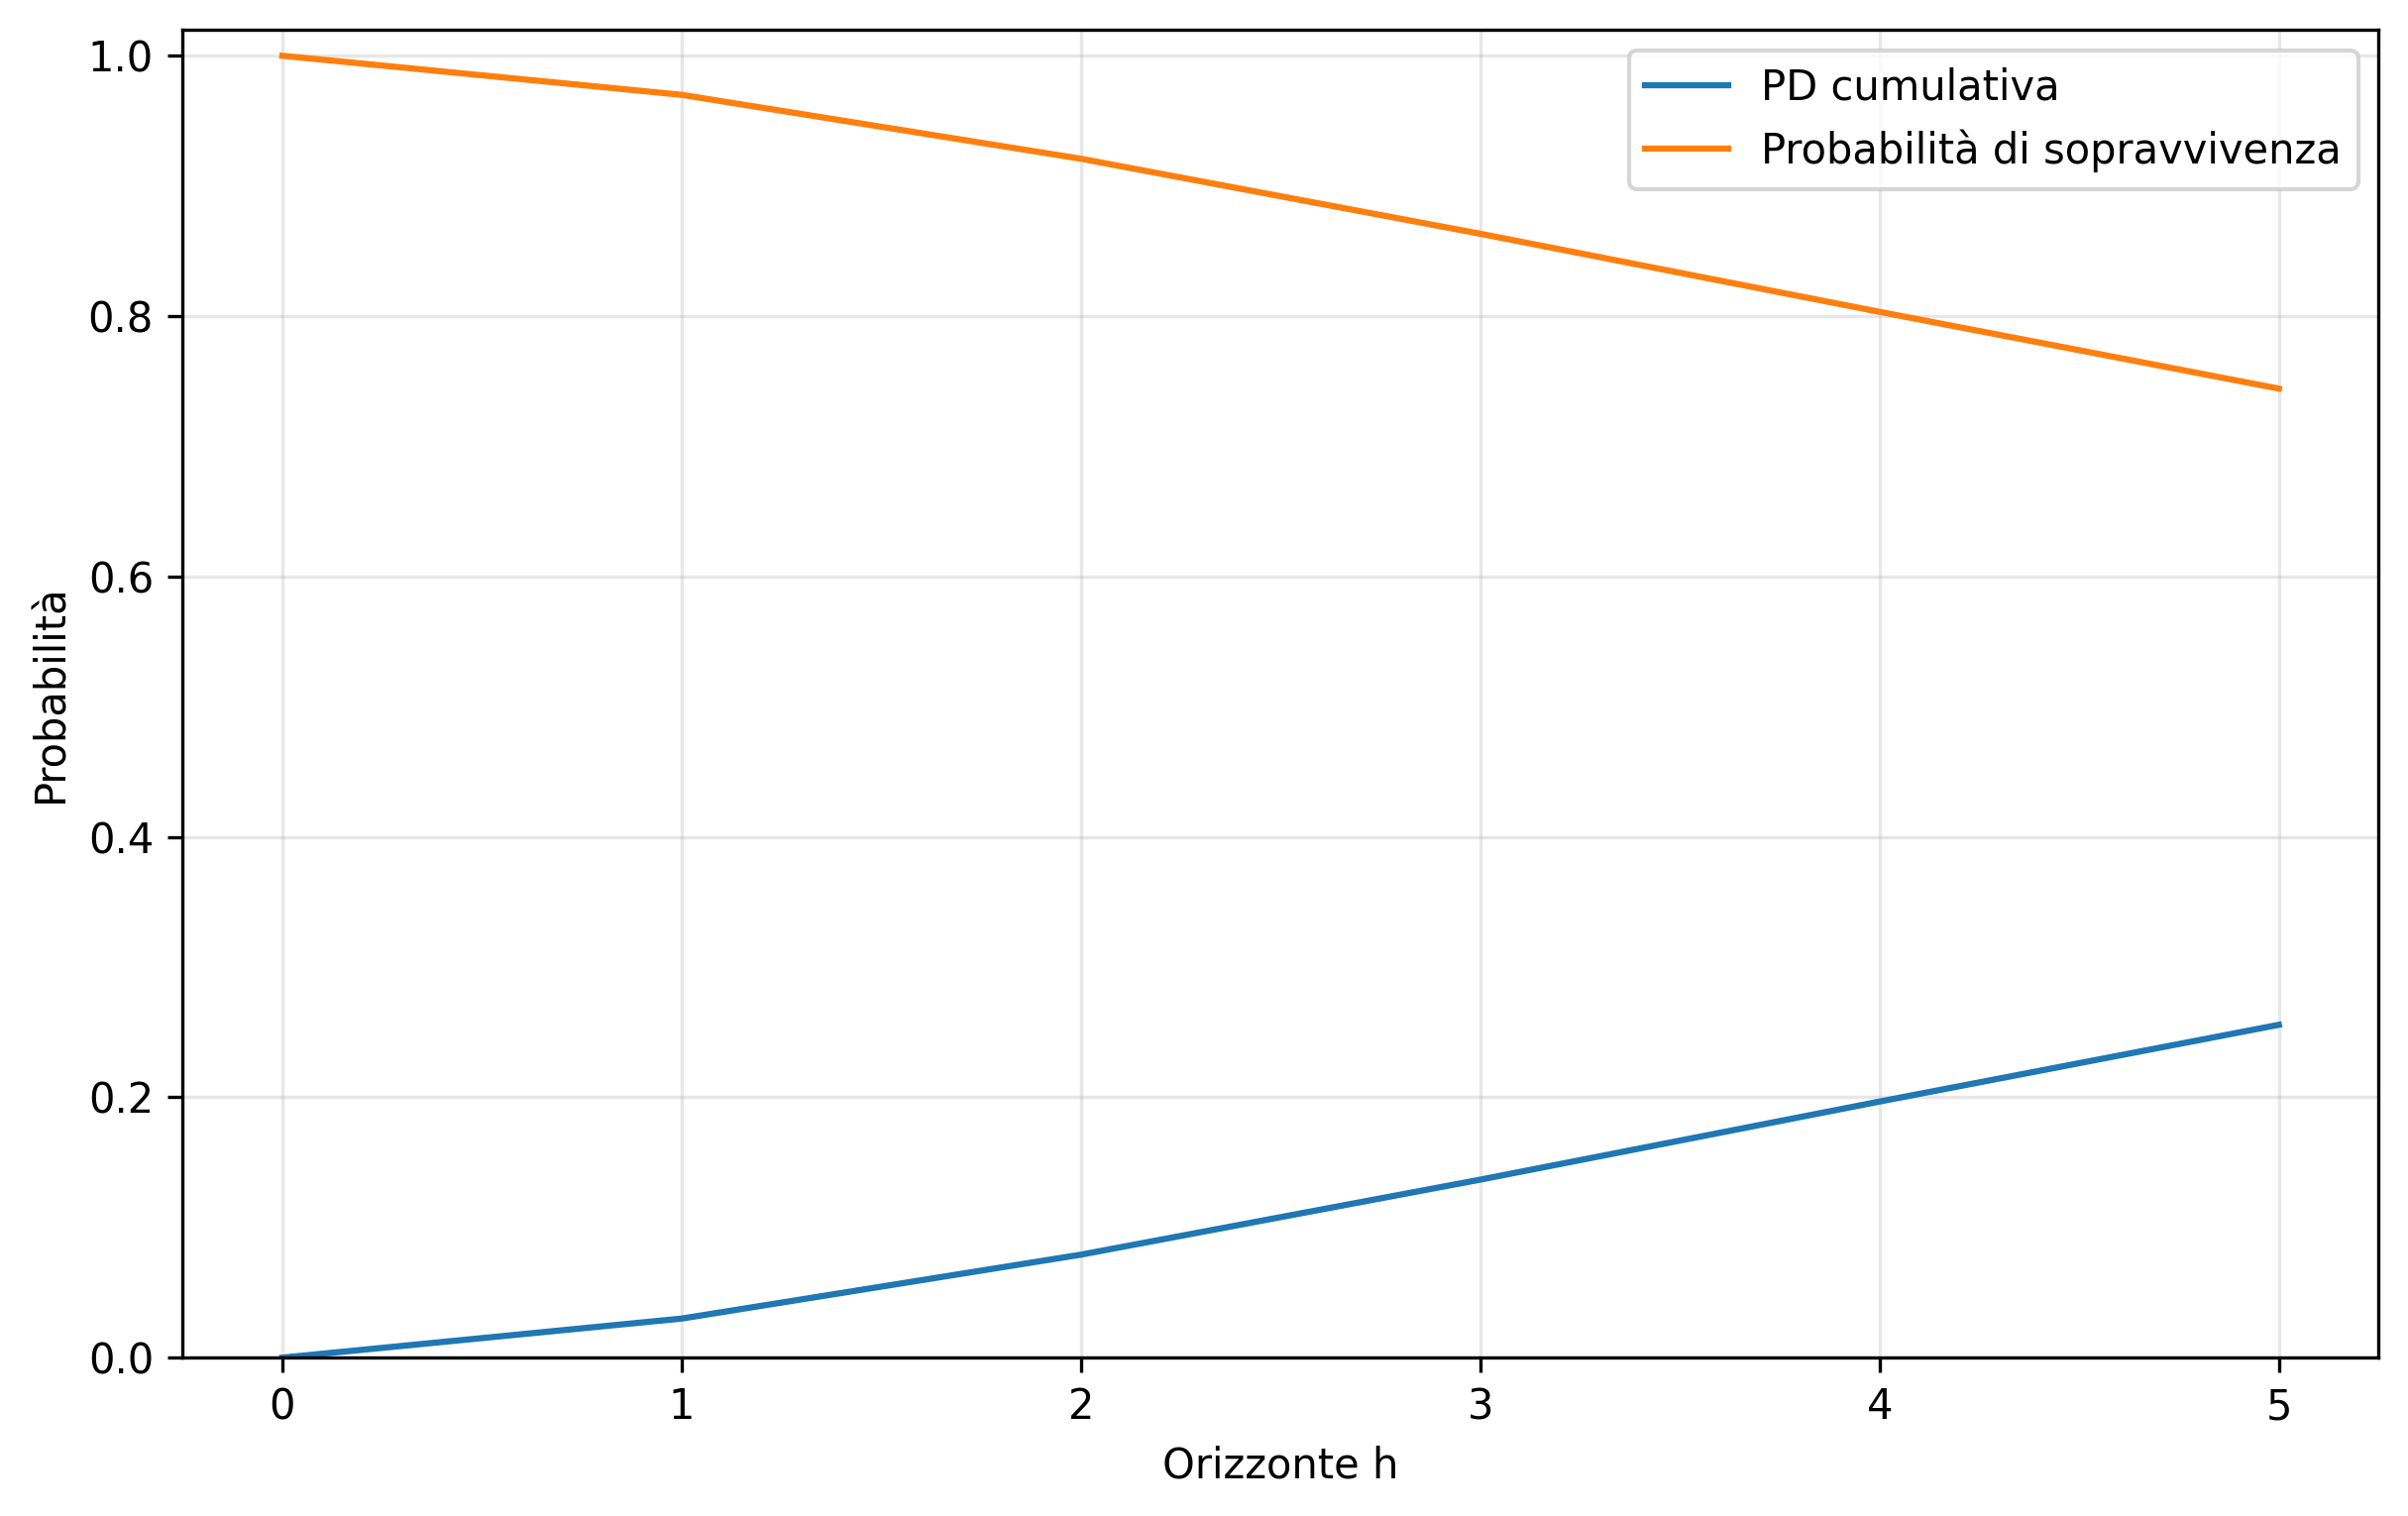
\includegraphics[width=0.78\textwidth]
{../graphics/Cap09_term_structure_default_esercizio.png}
\caption{Term structure della probabilit\`{a} cumulativa di default e
della probabilit\`{a} di sopravvivenza, condizionatamente al rating
iniziale $X_0=2$. Le due quantit\`{a} sono complementari a ogni
orizzonte.}
\label{fig:cap09-term-structure-default-esercizio}
\end{figure}

\item La probabilit\`{a} cumulativa di default cresce con l'orizzonte,
poich\'{e} incorpora tutti i possibili ingressi in default verificatisi
entro la data considerata. Simmetricamente, la probabilit\`{a} di
sopravvivenza diminuisce.

La probabilit\`{a} marginale misura invece il contributo del singolo
anno all'aumento della probabilit\`{a} cumulativa. Nel modello
considerato essa cresce nei primi quattro anni e si riduce lievemente
nel quinto.

La probabilit\`{a} condizionata di default aumenta dal $3\%$ del primo
anno a circa il $7.34\%$ del quinto anno. Il confronto con la
probabilit\`{a} marginale evidenzia l'effetto del condizionamento: il
rischio del singolo periodo viene misurato rispetto agli emittenti che
sono ancora sopravvissuti all'inizio del periodo stesso.

\end{enumerate}

\begin{exercise}[Distribuzione della perdita da migrazione]

\label{ex:cap09-distribuzione-perdita}

Si consideri un emittente inizialmente classificato nello stato
$X_0=2$. Dalla matrice di transizione dell'Esercizio precedente, la
distribuzione del rating dopo un anno \`{e}

\[
\begin{array}{c|cccc}
j & 1 & 2 & 3 & D\\
\hline
\Prob(X_1=j\mid X_0=2)
&
0.05
&
0.78
&
0.14
&
0.03
\end{array}
\]

Il valore di riferimento dell'esposizione alla data $h=1$ \`{e}

\[
V^{\mathrm{ref}}(h=1)=100.
\]

Ai quattro possibili rating futuri vengono associati i valori

\[
\begin{array}{c|cccc}
j & 1 & 2 & 3 & D\\
\hline
V_j(1)
&
104
&
100
&
90
&
45
\end{array}
\]

Si definisce la perdita a un anno mediante

\[
L_1=\ell(X_1,1),
\]

dove

\[
\ell(j,1)
=
V^{\mathrm{ref}}(1)-V_j(1).
\]

Condizionatamente al valore iniziale $X_0=2$:

\begin{enumerate}

\item Determinare la perdita associata a ciascun rating futuro.

\item Costruire la funzione di massa della variabile casuale $L_1$.

\item Determinare la funzione di ripartizione $F_{L_1}$.

\item Calcolare la perdita attesa.

\item Calcolare il momento secondo della perdita.

\item Calcolare la varianza e la deviazione standard.

\item Interpretare economicamente la distribuzione e i contributi dei
diversi stati alla perdita attesa.

\end{enumerate}

\end{exercise}

\noindent
\textbf{Soluzione.}

\begin{enumerate}

\item La funzione di perdita associa a ciascuno stato futuro la
differenza tra il valore di riferimento e il valore dell'esposizione
nello stato considerato:

\[
\ell(j,1)
=
V^{\mathrm{ref}}(1)-V_j(1).
\]

Si ottiene:

\[
\begin{array}{c|cccc}
j & 1 & 2 & 3 & D\\
\hline
V_j(1)
&
104
&
100
&
90
&
45
\\
\ell(j,1)
&
-4
&
0
&
10
&
55
\end{array}
\]

Pertanto,

\[
L_1
=
\begin{cases}
-4 & \text{se }X_1=1,\\
0  & \text{se }X_1=2,\\
10 & \text{se }X_1=3,\\
55 & \text{se }X_1=D.
\end{cases}
\]

La perdita negativa associata allo stato $1$ rappresenta un guadagno
rispetto al valore di riferimento: il miglioramento del rating
determina infatti un aumento del valore dell'esposizione.

\item La funzione di massa della perdita \`{e} ottenuta trasferendo le
probabilit\`{a} degli stati futuri sui corrispondenti valori di
perdita:

\[
\begin{array}{c|cccc}
\lambda
&
-4
&
0
&
10
&
55
\\
\hline
\Prob(L_1=\lambda\mid X_0=2)
&
0.05
&
0.78
&
0.14
&
0.03
\end{array}
\]

Le probabilit\`{a} sommano a uno:

\[
0.05+0.78+0.14+0.03=1.
\]

La Figura~\ref{fig:cap09-distribuzione-perdita-esercizio} rappresenta
la funzione di massa della perdita.

\begin{figure}[htbp]
\centering
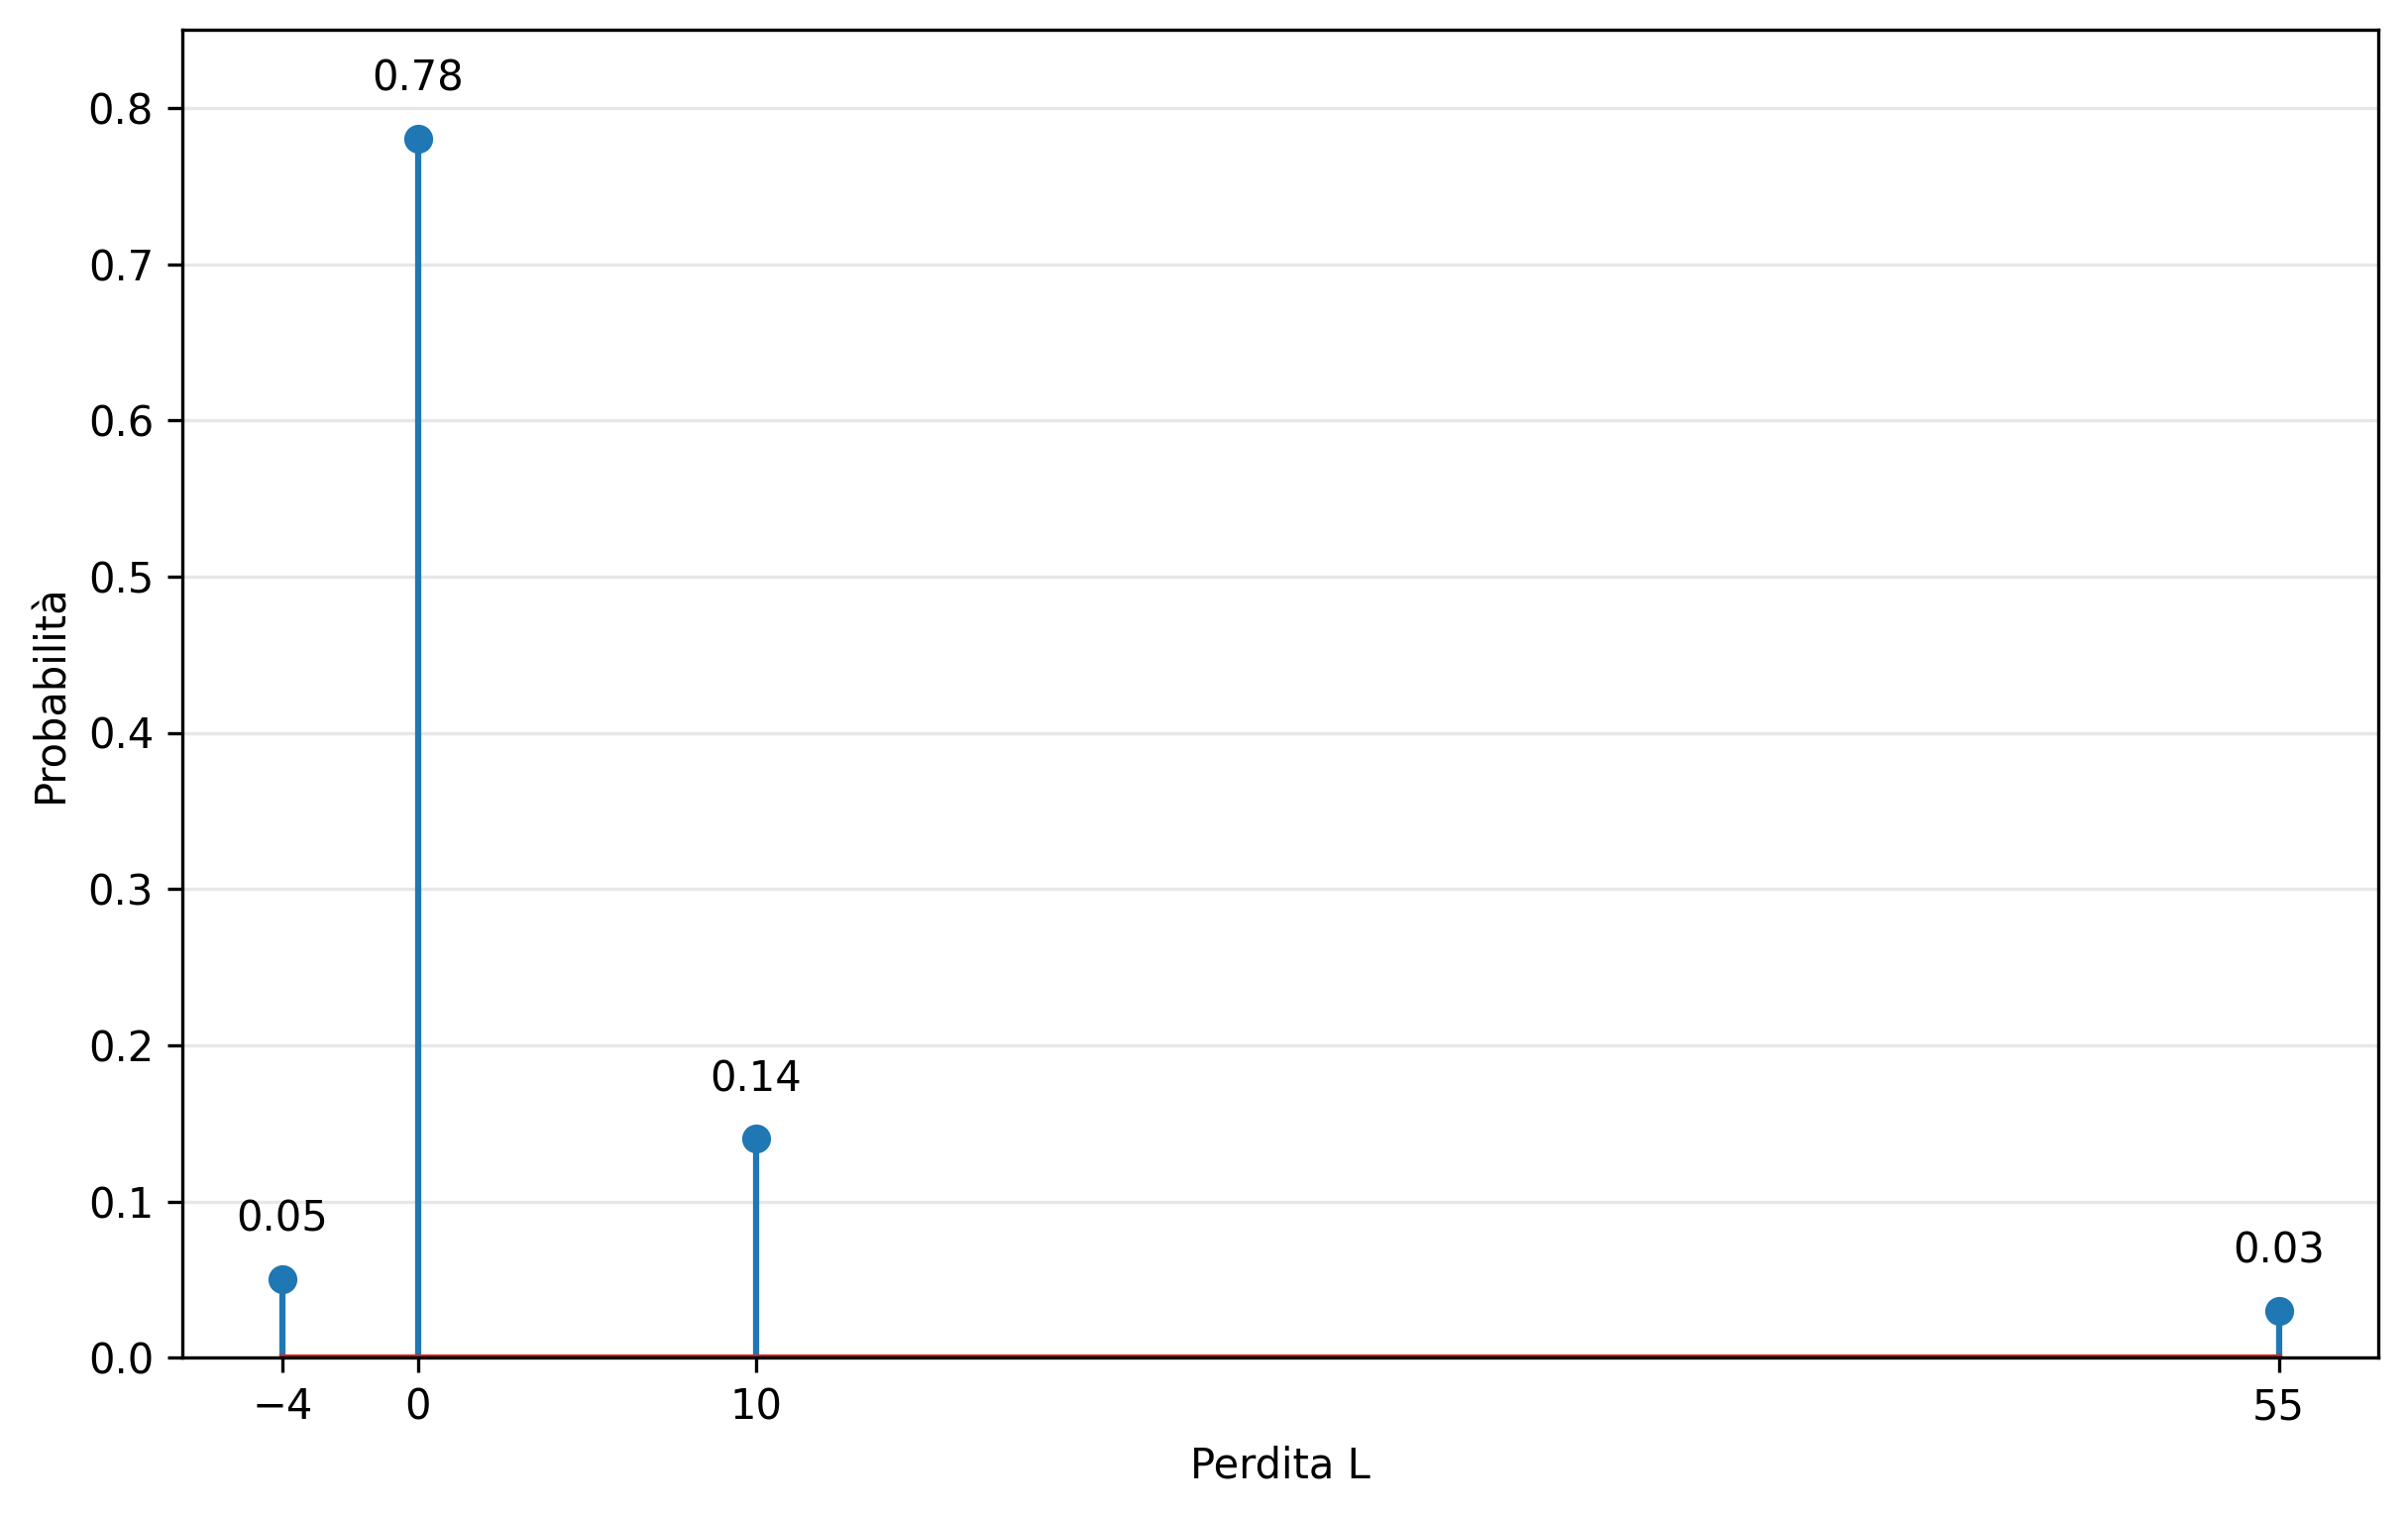
\includegraphics[width=0.78\textwidth]
{../graphics/Cap09_distribuzione_perdita_esercizio.png}
\caption{Funzione di massa della perdita a un anno associata alla
migrazione del rating. La maggior parte della probabilit\`{a} \`{e}
concentrata sulla perdita nulla, mentre il default genera una perdita
elevata ma poco probabile.}
\label{fig:cap09-distribuzione-perdita-esercizio}
\end{figure}

\item La funzione di ripartizione \`{e}

\[
F_{L_1}(\lambda)
=
\Prob(L_1\leq\lambda\mid X_0=2).
\]

Ordinando i possibili valori della perdita,

\[
-4<0<10<55,
\]

si ottiene:

\[
F_{L_1}(\lambda)
=
\begin{cases}
0
&
\text{se }\lambda<-4,
\\
0.05
&
\text{se }-4\leq\lambda<0,
\\
0.83
&
\text{se }0\leq\lambda<10,
\\
0.97
&
\text{se }10\leq\lambda<55,
\\
1
&
\text{se }\lambda\geq55.
\end{cases}
\]

In corrispondenza dei quattro valori della perdita:

\[
\begin{array}{c|cccc}
\lambda
&
-4
&
0
&
10
&
55
\\
\hline
F_{L_1}(\lambda)
&
0.05
&
0.83
&
0.97
&
1
\end{array}
\]

\item La perdita attesa, condizionatamente al rating iniziale, \`{e}

\[
\E^{\Prob}[L_1\mid X_0=2]
=
\sum_{j\in\mathcal{I}}
\ell(j,1)
\Prob(X_1=j\mid X_0=2).
\]

Sostituendo i valori:

\[
\begin{split}
\mathrm{EL}_2(1)
&=
(-4)(0.05)
+
(0)(0.78)
\\
&\quad
+
(10)(0.14)
+
(55)(0.03)
\\
&=
-0.20+0+1.40+1.65
\\
&=
2.85.
\end{split}
\]

Esplicitando i contributi economici:

\[
\begin{split}
\mathrm{EL}_2(1)
&=
\underbrace{(-4)(0.05)}_{\text{upgrade}}
+
\underbrace{(0)(0.78)}_{\text{permanenza}}
\\
&\quad
+
\underbrace{(10)(0.14)}_{\text{downgrade}}
+
\underbrace{(55)(0.03)}_{\text{default}}.
\end{split}
\]

La perdita attesa a un anno \`{e} quindi pari a

\[
\boxed{\mathrm{EL}_2(1)=2.85}.
\]

\item Il momento secondo \`{e}

\[
\E^{\Prob}[L_1^2\mid X_0=2]
=
\sum_{\lambda}
\lambda^2
\Prob(L_1=\lambda\mid X_0=2).
\]

Pertanto,

\[
\begin{split}
\E^{\Prob}[L_1^2\mid X_0=2]
&=
(-4)^2(0.05)
+
0^2(0.78)
\\
&\quad
+
10^2(0.14)
+
55^2(0.03)
\\
&=
16(0.05)
+
100(0.14)
+
3025(0.03)
\\
&=
0.80+14+90.75
\\
&=
105.55.
\end{split}
\]

\item La varianza si ottiene dalla relazione

\[
\Var(L_1\mid X_0=2)
=
\E^{\Prob}[L_1^2\mid X_0=2]
-
\left(
\E^{\Prob}[L_1\mid X_0=2]
\right)^2.
\]

Quindi,

\[
\begin{split}
\Var(L_1\mid X_0=2)
&=
105.55-(2.85)^2
\\
&=
105.55-8.1225
\\
&=
97.4275.
\end{split}
\]

La deviazione standard \`{e}

\[
\begin{split}
\sigma_{L_1}
&=
\sqrt{\Var(L_1\mid X_0=2)}
\\
&=
\sqrt{97.4275}
\\
&\approx
9.87.
\end{split}
\]

\item La distribuzione \`{e} fortemente asimmetrica. Con probabilit\`{a}

\[
0.05+0.78=0.83
\]

l'emittente migliora il proprio rating oppure rimane nella classe
iniziale, producendo una perdita non positiva. La probabilit\`{a} di
una perdita strettamente positiva \`{e} invece

\[
\Prob(L_1>0\mid X_0=2)
=
0.14+0.03
=
0.17.
\]

Il downgrade produce una perdita moderata pari a $10$, mentre il
default produce una perdita molto pi\`{u} elevata, pari a $55$.

Nonostante la probabilit\`{a} di default sia soltanto del $3\%$, il suo
contributo alla perdita attesa \`{e}

\[
55(0.03)=1.65,
\]

superiore al contributo del downgrade:

\[
10(0.14)=1.40.
\]

Il default domina ancora pi\`{u} nettamente il momento secondo:

\[
55^2(0.03)=90.75,
\]

su un valore complessivo pari a $105.55$. La dispersione della perdita
dipende quindi soprattutto dalla presenza di un evento raro ma di
grande severit\`{a}.

\end{enumerate}

\begin{exercise}[VaR e CVaR di una distribuzione discreta]

\label{ex:cap09-var-cvar-discreti}

Si riprenda la distribuzione della perdita a un anno costruita
nell'Esercizio~\ref{ex:cap09-distribuzione-perdita}:

\[
\begin{array}{c|cccc}
\lambda
&
-4
&
0
&
10
&
55
\\
\hline
\Prob(L_1=\lambda\mid X_0=2)
&
0.05
&
0.78
&
0.14
&
0.03
\end{array}
\]

Si consideri il livello di confidenza

\[
\alpha=0.95.
\]

\begin{enumerate}

\item Determinare il $\VaR_{0.95}(L_1)$.

\item Individuare la coda peggiore di probabilit\`{a} $1-\alpha=0.05$
e stabilire quale parte della massa collocata nel punto quantilico
deve essere inclusa nella coda.

\item Calcolare il $\CVaR_{0.95}(L_1)$ come media delle perdite
appartenenti alla coda peggiore del $5\%$.

\item Verificare il risultato mediante la rappresentazione

\[
\CVaR_{\alpha}(L)
=
\min_{\eta\in\R}
\left\{
\eta
+
\frac{1}{1-\alpha}
\E^{\Prob}
\left[
(L-\eta)^{+}
\right]
\right\}.
\]

\item Calcolare

\[
\E^{\Prob}
\left[
L_1
\mid
L_1\geq\VaR_{0.95}(L_1),\ X_0=2
\right]
\]

e spiegare perch\'{e} tale valore non coincide con il
$\CVaR_{0.95}(L_1)$.

\end{enumerate}

\end{exercise}

\noindent
\textbf{Soluzione.}

\begin{enumerate}

\item La funzione di ripartizione della perdita assume, nei punti del
supporto, i valori

\[
\begin{array}{c|cccc}
\lambda
&
-4
&
0
&
10
&
55
\\
\hline
F_{L_1}(\lambda)
&
0.05
&
0.83
&
0.97
&
1
\end{array}
\]

Per definizione,

\[
\VaR_{0.95}(L_1)
=
\inf
\left\{
\lambda\in\R:
F_{L_1}(\lambda)\geq0.95
\right\}.
\]

Poich\'{e}

\[
F_{L_1}(0)=0.83<0.95
\]

e

\[
F_{L_1}(10)=0.97\geq0.95,
\]

si ottiene

\[
\boxed{
\VaR_{0.95}(L_1)=10
}.
\]

Il VaR indica quindi che il quantile di livello $0.95$ della
distribuzione della perdita \`{e} pari a $10$.

\item La coda peggiore deve avere probabilit\`{a}

\[
1-\alpha=0.05.
\]

Le perdite strettamente superiori al VaR comprendono soltanto il valore

\[
L_1=55,
\]

che ha probabilit\`{a}

\[
\Prob(L_1>10\mid X_0=2)=0.03.
\]

Per completare la coda peggiore del $5\%$ occorre quindi includere
un'ulteriore probabilit\`{a}

\[
0.05-0.03=0.02
\]

proveniente dalla massa collocata nel punto quantilico

\[
L_1=10.
\]

La massa complessiva in tale punto \`{e}

\[
\Prob(L_1=10\mid X_0=2)=0.14.
\]

Nella coda entra pertanto soltanto la quota

\[
\frac{0.02}{0.14}
=
\frac{1}{7}
\]

della massa associata alla perdita $10$. La restante probabilit\`{a}

\[
0.14-0.02=0.12
\]

rimane fuori dalla coda peggiore selezionata.

La composizione della coda \`{e} quindi

\[
\begin{array}{c|cc}
\text{perdita}
&
10
&
55
\\
\hline
\text{massa inclusa nella coda}
&
0.02
&
0.03
\end{array}
\]

e le corrispondenti probabilit\`{a} normalizzate sono

\[
\frac{0.02}{0.05}=0.40,
\qquad
\frac{0.03}{0.05}=0.60.
\]

La Figura~\ref{fig:cap09-cvar-massa-quantile-esercizio} mostra la
selezione della coda peggiore del $5\%$.

\begin{figure}[htbp]
\centering
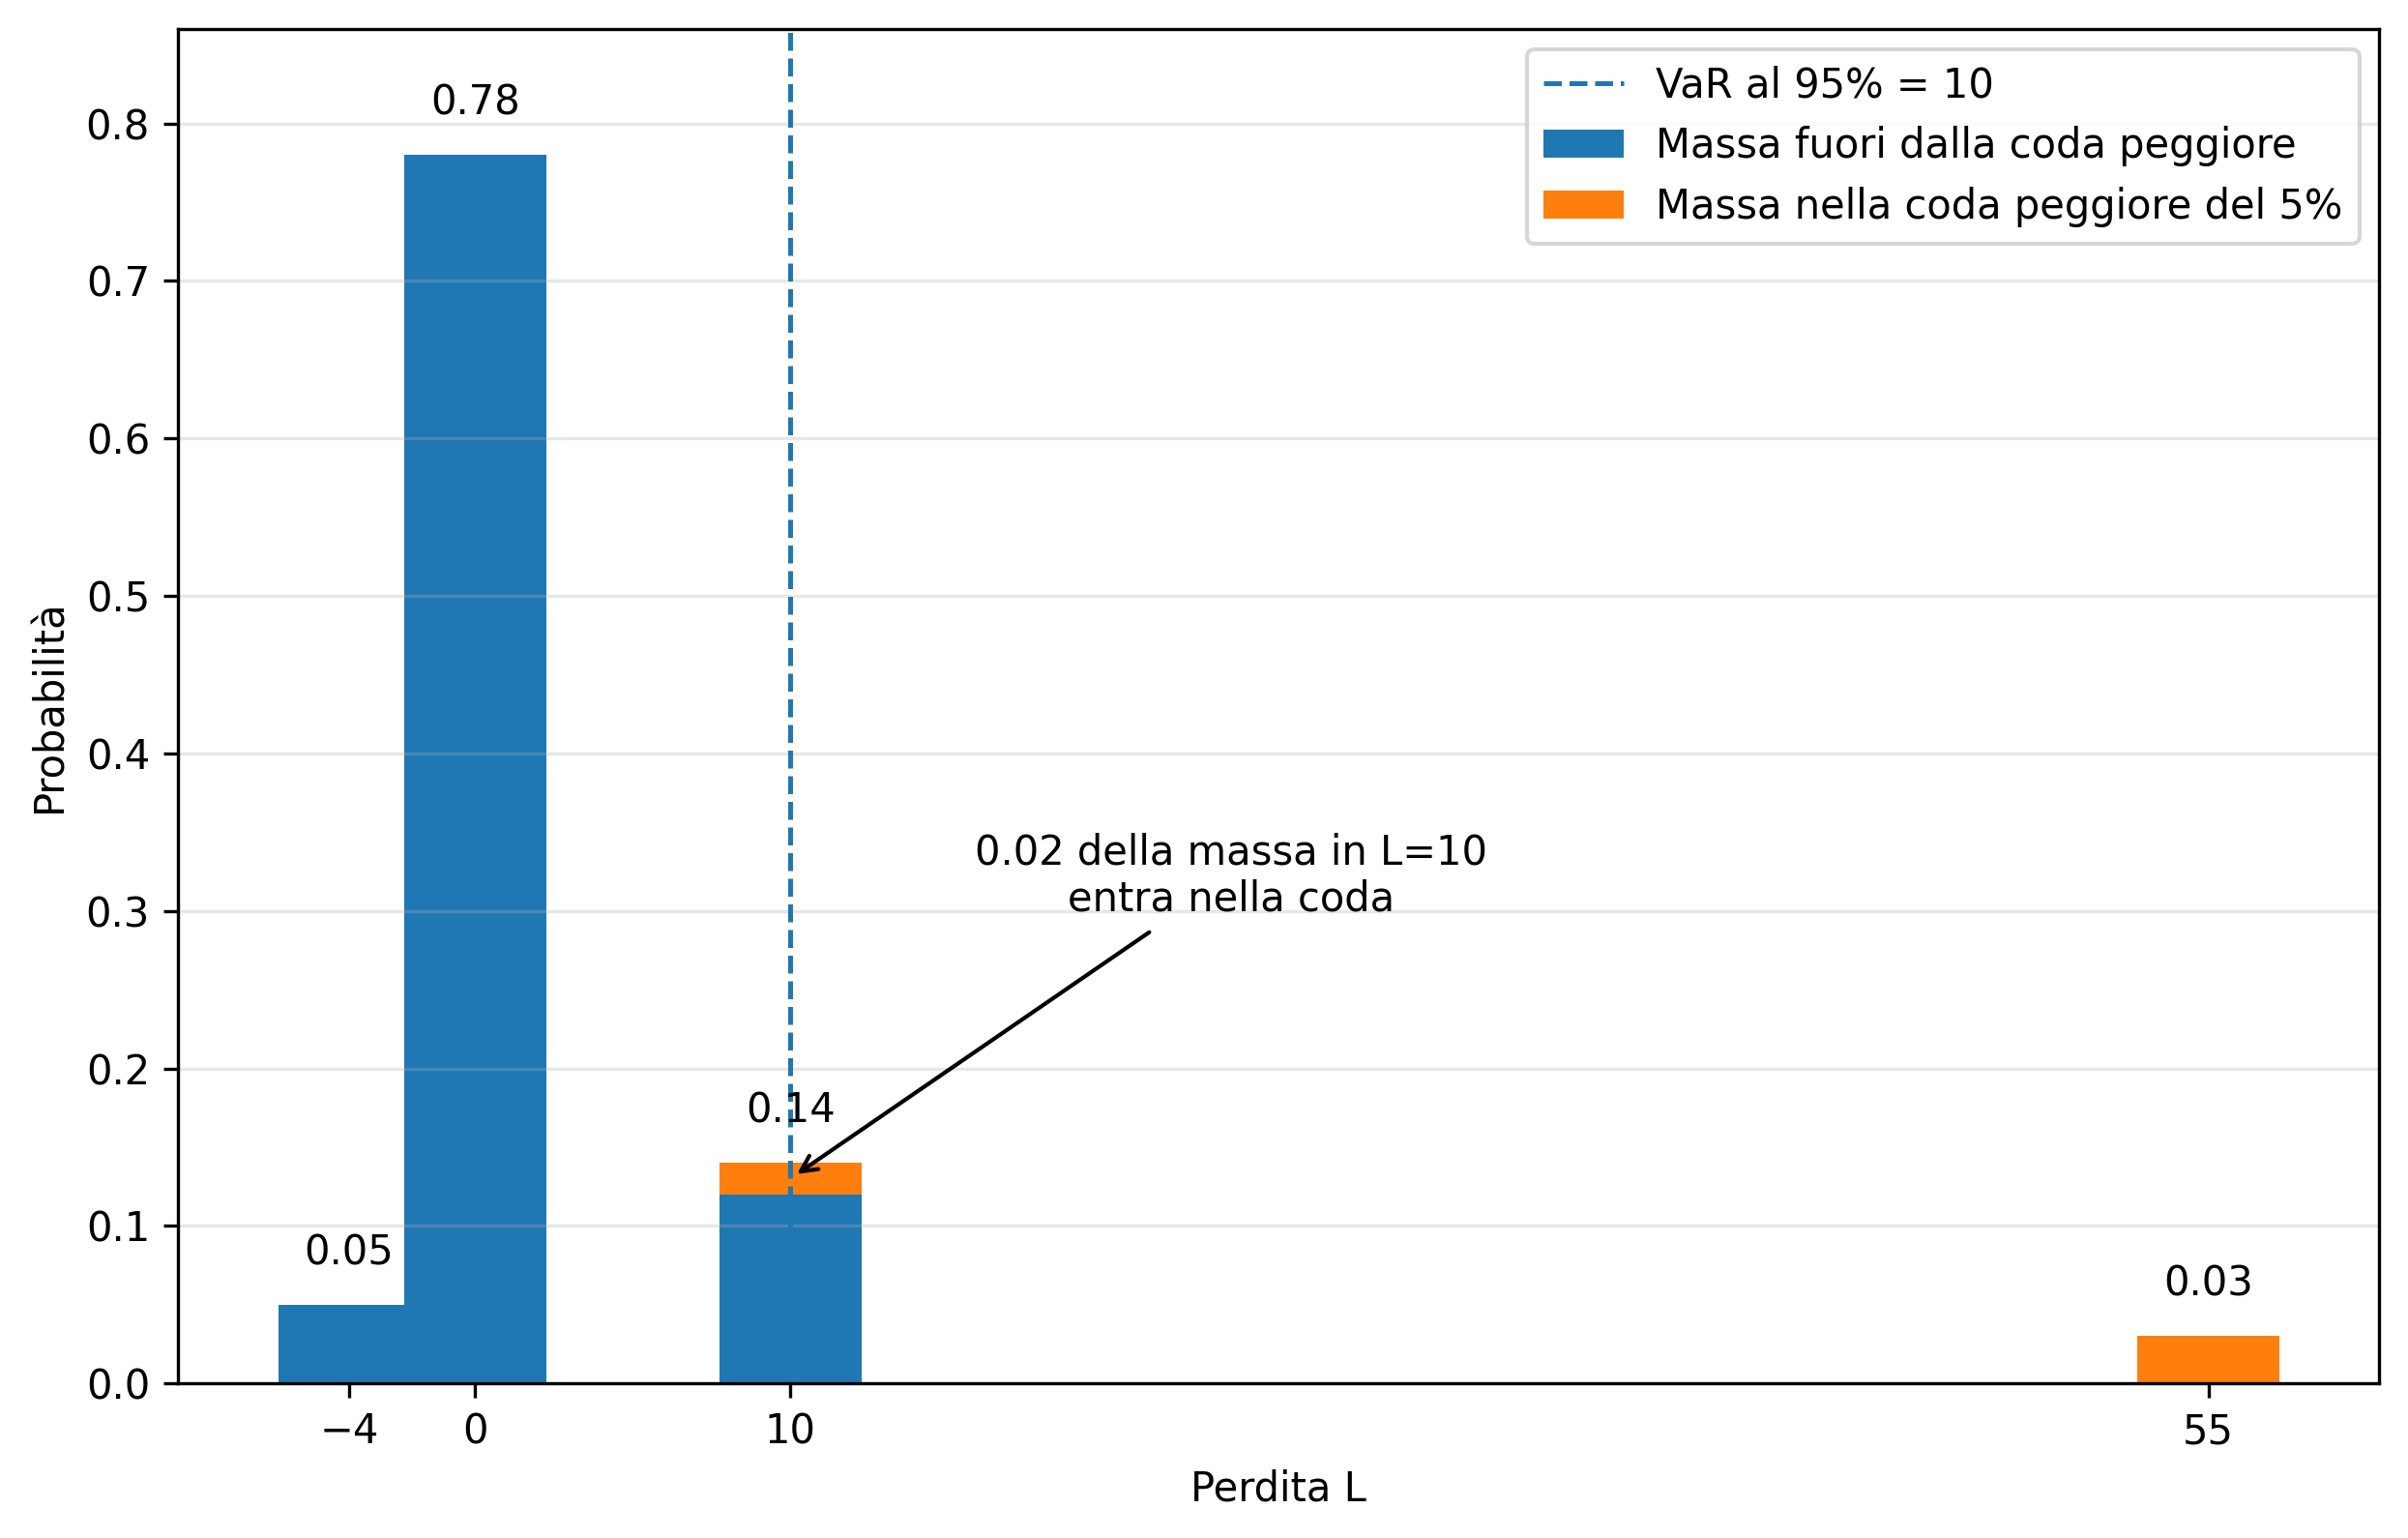
\includegraphics[width=0.82\textwidth]
{../graphics/Cap09_CVaR_massa_quantile_esercizio.png}
\caption{Composizione della coda peggiore del $5\%$. La coda comprende
tutta la massa associata alla perdita $55$ e soltanto una parte della
massa collocata nel punto quantilico $L_1=10$.}
\label{fig:cap09-cvar-massa-quantile-esercizio}
\end{figure}

\item Il CVaR \`{e} la media delle perdite appartenenti alla coda
peggiore, dopo avere normalizzato le masse rispetto alla probabilit\`{a}
complessiva della coda:

\[
\begin{split}
\CVaR_{0.95}(L_1)
&=
10
\frac{0.02}{0.05}
+
55
\frac{0.03}{0.05}
\\
&=
10(0.40)+55(0.60)
\\
&=
4+33
\\
&=
37.
\end{split}
\]

Pertanto,

\[
\boxed{
\CVaR_{0.95}(L_1)=37
}.
\]

Il CVaR \`{e} nettamente superiore al VaR:

\[
\CVaR_{0.95}(L_1)=37
>
10=\VaR_{0.95}(L_1),
\]

poich\'{e} incorpora anche la perdita estrema pari a $55$.

\item Nella rappresentazione basata sulla parte positiva, poniamo

\[
\eta=\VaR_{0.95}(L_1)=10.
\]

Si ha

\[
(L_1-10)^{+}
=
\begin{cases}
0 & \text{se }L_1=-4,\\
0 & \text{se }L_1=0,\\
0 & \text{se }L_1=10,\\
45 & \text{se }L_1=55.
\end{cases}
\]

Pertanto,

\[
\begin{split}
\E^{\Prob}
\left[
(L_1-10)^{+}
\mid X_0=2
\right]
&=
45(0.03)
\\
&=
1.35.
\end{split}
\]

Sostituendo nella formula:

\[
\begin{split}
\CVaR_{0.95}(L_1)
&=
10
+
\frac{1}{1-0.95}(1.35)
\\
&=
10+20(1.35)
\\
&=
10+27
\\
&=
37.
\end{split}
\]

Si ritrova quindi lo stesso risultato:

\[
\boxed{
\CVaR_{0.95}(L_1)=37
}.
\]

La massa parzialmente selezionata al quantile di livello $0.95$ non
compare esplicitamente nel termine

\[
\E^{\Prob}[(L_1-\eta)^{+}],
\]

poich\'{e} per $L_1=\eta=10$ la parte positiva \`{e} nulla. Il suo
effetto \`{e} incorporato nel termine iniziale $\eta$ della
rappresentazione.

\item L'evento

\[
\left\{
L_1\geq\VaR_{0.95}(L_1)
\right\}
\]

comprende tutta la massa associata alle perdite $10$ e $55$. La sua
probabilit\`{a} \`{e}

\[
\Prob(L_1\geq10\mid X_0=2)
=
0.14+0.03
=
0.17.
\]

Il corrispondente valore atteso condizionato \`{e}

\[
\begin{split}
\E^{\Prob}
\left[
L_1
\mid
L_1\geq10,\ X_0=2
\right]
&=
\frac{
10(0.14)+55(0.03)
}{
0.17
}
\\
&=
\frac{1.40+1.65}{0.17}
\\
&=
\frac{3.05}{0.17}
\\
&\approx
17.94.
\end{split}
\]

Si ottiene quindi

\[
\E^{\Prob}
\left[
L_1
\mid
L_1\geq\VaR_{0.95}(L_1),\ X_0=2
\right]
\approx
17.94,
\]

mentre

\[
\CVaR_{0.95}(L_1)=37.
\]

Le due quantit\`{a} non coincidono perch\'{e} l'evento

\[
\{L_1\geq10\}
\]

ha probabilit\`{a} $0.17$, mentre la coda richiesta per il calcolo del
CVaR deve avere probabilit\`{a} esattamente pari a $0.05$.

Il valore atteso condizionato include tutta la massa $0.14$ collocata
nel punto quantilico. Il CVaR include invece soltanto la quota $0.02$
necessaria a completare la coda peggiore del $5\%$.

In presenza di distribuzioni discrete, pertanto,

\[
\CVaR_{\alpha}(L)
\neq
\E^{\Prob}
\left[
L
\mid
L\geq\VaR_{\alpha}(L)
\right]
\]

in generale.

\end{enumerate}

\begin{exercise}[Sensibilit\`{a} dello spread equo di un CDS]

\label{ex:cap09-sensibilita-spread-cds}

Si consideri un CDS con nozionale

\[
N=100
\]

e scadenza $H=3$. I fattori di sconto sono

\[
d_1=0.98,
\qquad
d_2=0.95,
\qquad
d_3=0.92.
\]

Nel primo scenario, le probabilit\`{a} marginali risk-neutral di
default sono

\[
\Prob^{\Q}(\tau_D=1)=0.03,
\qquad
\Prob^{\Q}(\tau_D=2)=0.04,
\qquad
\Prob^{\Q}(\tau_D=3)=0.05.
\]

Le probabilit\`{a} di sopravvivenza sono pertanto

\[
\Prob^{\Q}(\tau_D>1)=0.97,
\qquad
\Prob^{\Q}(\tau_D>2)=0.93,
\qquad
\Prob^{\Q}(\tau_D>3)=0.88.
\]

Si assume che il premio alla data $h$ venga pagato soltanto se
$\tau_D>h$.

\begin{enumerate}

\item Con recovery rate $R=0.40$, calcolare il valore attuale della
gamba di protezione e il coefficiente della gamba dei premi.

\item Determinare lo spread equo $s^*$.

\item Ripetere il calcolo per $R=0.30$ e $R=0.50$, mantenendo
invariate le probabilit\`{a} risk-neutral.

\item Considerare un secondo scenario con probabilit\`{a} marginali
risk-neutral

\[
0.04,
\qquad
0.05,
\qquad
0.07.
\]

Calcolare il nuovo spread equo per $R=0.40$.

\item Interpretare separatamente l'effetto del recovery rate e quello
delle probabilit\`{a} risk-neutral.
\end{enumerate}
\end{exercise}

\noindent
\textbf{Soluzione.}

\begin{enumerate}

\item Introduciamo il fattore attualizzato associato alla gamba di
protezione:

\[
A_{\mathrm{prot}}
=
\sum_{h=1}^{3}
d_h
\Prob^{\Q}(\tau_D=h).
\]

Sostituendo i dati:

\[
\begin{split}
A_{\mathrm{prot}}
&=
(0.98)(0.03)
+
(0.95)(0.04)
+
(0.92)(0.05)
\\
&=
0.0294+0.0380+0.0460
\\
&=
0.1134.
\end{split}
\]

Il valore attuale della gamba di protezione, per $R=0.40$, \`{e}

\[
\begin{split}
\mathrm{PV}_{\mathrm{prot}}
&=
N(1-R)A_{\mathrm{prot}}
\\
&=
100(0.60)(0.1134)
\\
&=
6.804.
\end{split}
\]

Per la gamba dei premi definiamo

\[
A_{\mathrm{prem}}
=
\sum_{h=1}^{3}
d_h
\Prob^{\Q}(\tau_D>h).
\]

Si ottiene:

\[
\begin{split}
A_{\mathrm{prem}}
&=
(0.98)(0.97)
+
(0.95)(0.93)
+
(0.92)(0.88)
\\
&=
0.9506+0.8835+0.8096
\\
&=
2.6437.
\end{split}
\]

Pertanto,

\[
\mathrm{PV}_{\mathrm{prem}}(s)
=
sNA_{\mathrm{prem}}
=
264.37s.
\]

\item Lo spread equo $s^{*}$ rende uguali i valori attuali delle due
gambe:

\[
\mathrm{PV}_{\mathrm{prot}}
=
\mathrm{PV}_{\mathrm{prem}}(s^{*}).
\]

Quindi,

\[
6.804
=
264.37s^{*},
\]

da cui

\[
s^{*}
=
\frac{6.804}{264.37}
\approx
0.02574.
\]

Lo spread equo annuale \`{e} quindi circa

\[
\boxed{
s^{*}=2.574\%
}
\]

ossia

\[
\boxed{
s^{*}\approx257.4\text{ punti base}.
}
\]

Il nozionale compare in entrambe le gambe e si semplifica nella
determinazione dello spread:

\[
s^{*}
=
(1-R)
\frac{
A_{\mathrm{prot}}
}{
A_{\mathrm{prem}}
}.
\]

\begin{figure}[htbp]
\centering
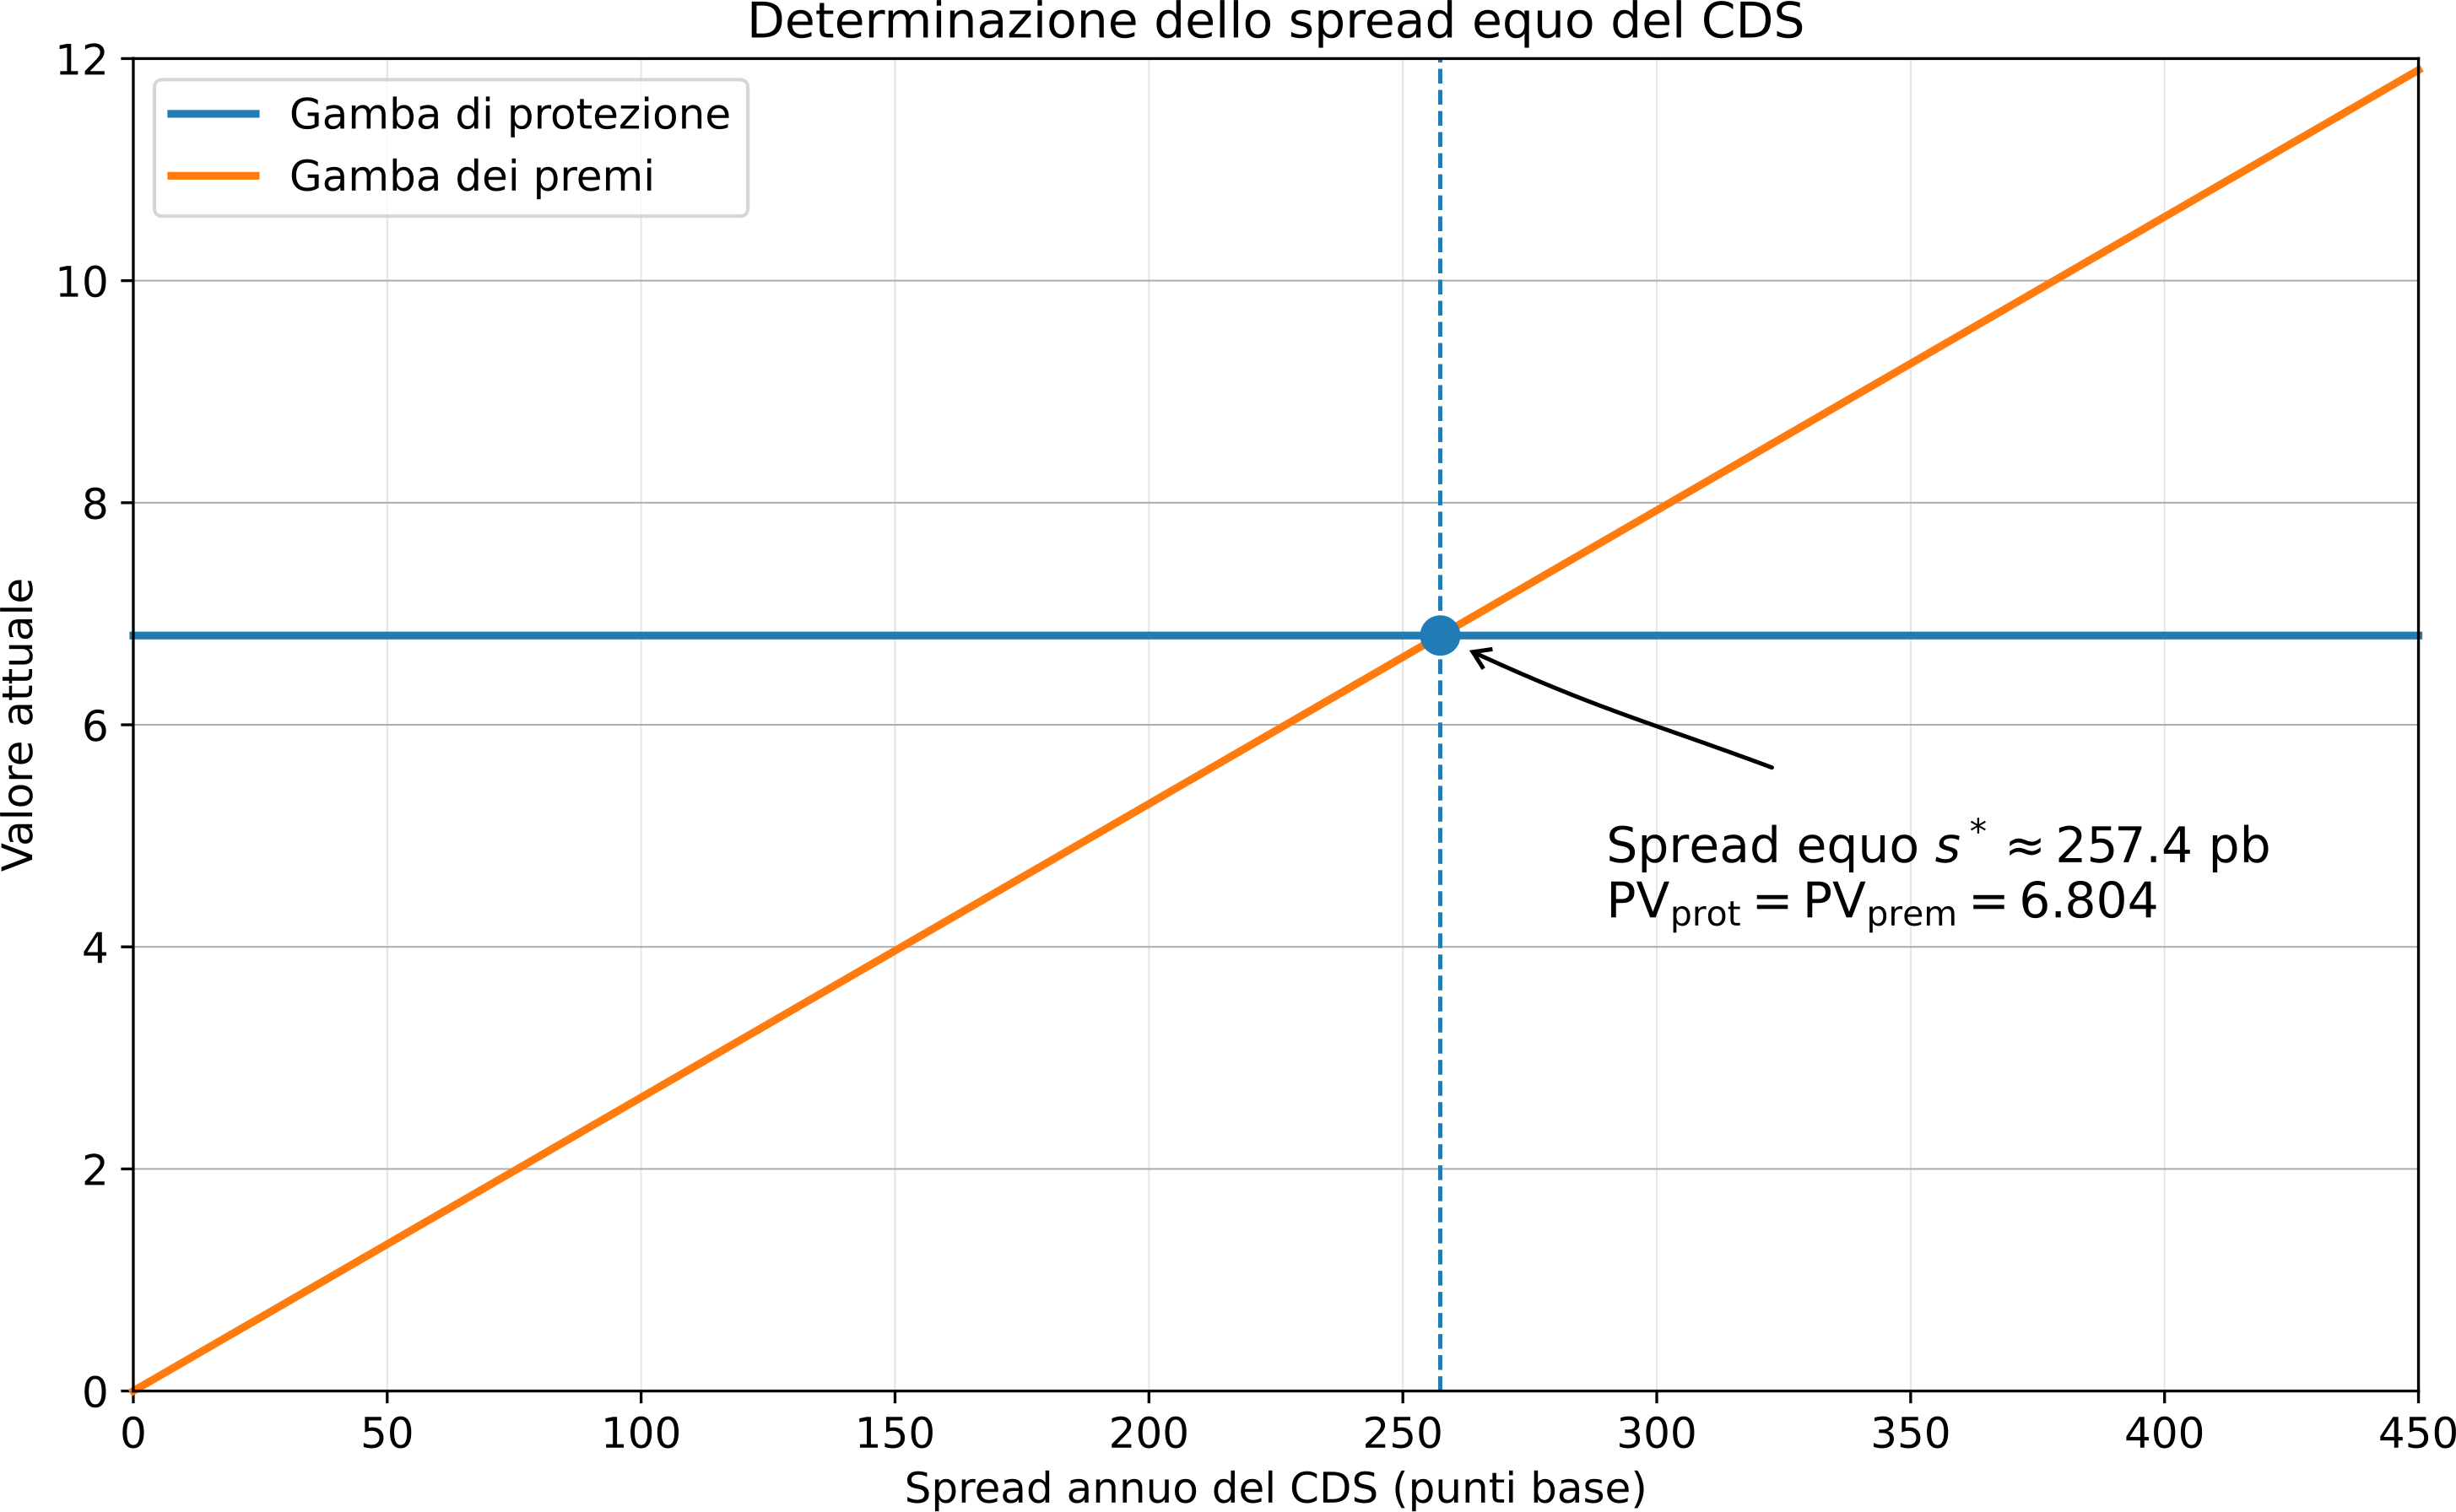
\includegraphics[width=0.90\textwidth]
{../graphics/Cap09_CDS_equilibrio_gambe.png}
\caption{Determinazione dello spread equo del CDS. Il valore attuale
della gamba di protezione non dipende dallo spread contrattuale,
mentre il valore attuale della gamba dei premi cresce linearmente con
esso. Il punto di intersezione identifica lo spread equo
$s^{*}\approx257.4$ punti base, per il quale le due gambe hanno valore
attuale pari a $6.804$.}
\label{fig:cap09-cds-equilibrio-gambe}
\end{figure}

\item Mantenendo invariate le probabilit\`{a} risk-neutral e i fattori
di sconto, la sensibilit\`{a} rispetto al recovery rate \`{e}

\[
s^{*}(R)
=
(1-R)
\frac{0.1134}{2.6437}.
\]

Per $R=0.30$:

\[
\begin{split}
s^{*}(0.30)
&=
0.70
\frac{0.1134}{2.6437}
\\
&\approx
0.03003,
\end{split}
\]

ossia circa

\[
\boxed{
300.3\text{ punti base}.
}
\]

Per $R=0.50$:

\[
\begin{split}
s^{*}(0.50)
&=
0.50
\frac{0.1134}{2.6437}
\\
&\approx
0.02145,
\end{split}
\]

ossia circa

\[
\boxed{
214.5\text{ punti base}.
}
\]

A parit\`{a} delle altre condizioni, un recovery rate pi\`{u} elevato
riduce il pagamento atteso della protezione e quindi riduce lo spread
equo.

\item Nel secondo scenario, le probabilit\`{a} marginali risk-neutral
di default sono

\[
0.04,
\qquad
0.05,
\qquad
0.07.
\]

Le corrispondenti probabilit\`{a} di sopravvivenza sono:

\[
\Prob^{\Q}(\tau_D>1)=0.96,
\]

\[
\Prob^{\Q}(\tau_D>2)
=
1-0.04-0.05
=
0.91,
\]

e

\[
\Prob^{\Q}(\tau_D>3)
=
1-0.04-0.05-0.07
=
0.84.
\]

Il nuovo fattore della gamba di protezione \`{e}

\[
\begin{split}
A_{\mathrm{prot}}^{(2)}
&=
(0.98)(0.04)
+
(0.95)(0.05)
+
(0.92)(0.07)
\\
&=
0.0392+0.0475+0.0644
\\
&=
0.1511.
\end{split}
\]

Il fattore della gamba dei premi \`{e}

\[
\begin{split}
A_{\mathrm{prem}}^{(2)}
&=
(0.98)(0.96)
+
(0.95)(0.91)
+
(0.92)(0.84)
\\
&=
0.9408+0.8645+0.7728
\\
&=
2.5781.
\end{split}
\]

Con $R=0.40$:

\[
\begin{split}
s^{*}_{2}
&=
0.60
\frac{0.1511}{2.5781}
\\
&\approx
0.03517.
\end{split}
\]

Il nuovo spread equo \`{e} quindi

\[
\boxed{
s^{*}_{2}\approx351.7\text{ punti base}.
}
\]

\item Il recovery rate incide sulla severit\`{a} del pagamento di
protezione:

\[
N(1-R).
\]

Mantenendo fisse le probabilit\`{a} risk-neutral, una riduzione di $R$
aumenta quindi lo spread equo.

Un aumento delle probabilit\`{a} risk-neutral di default produce invece
due effetti:

\begin{itemize}

\item aumenta il valore attuale della gamba di protezione;

\item riduce le probabilit\`{a} di sopravvivenza e quindi il valore della
gamba dei premi per ogni unit\`{a} di spread.

\end{itemize}

Entrambi gli effetti determinano un aumento dello spread equo. I
confronti precedenti sono esercizi di sensibilit\`{a} parziale: ogni
parametro viene modificato mantenendo invariati gli altri dati del
modello.

\end{enumerate}

\section{Esercizi proposti}

\label{sec:cap09-esercizi-proposti}

Gli esercizi seguenti riprendono le principali componenti della catena
di misurazione sviluppata nel capitolo. Le applicazioni procedono dal
confronto tra differenti rappresentazioni della perdita creditizia
alla misurazione del rischio di portafoglio e agli scenari di stress.

\begin{exercise}[Modello default-only e modello migration-based]

\label{ex:cap09-default-only-migration-based}

Si considerino due emittenti, $A$ e $B$, inizialmente appartenenti alla
classe di rating $2$. Dopo un anno, le rispettive distribuzioni dei
rating sono:

\[
\begin{array}{c|cccc}
&
1
&
2
&
3
&
D
\\
\hline
A
&
0.08
&
0.75
&
0.14
&
0.03
\\
B
&
0.02
&
0.70
&
0.25
&
0.03
\end{array}
\]

I valori della perdita associati ai quattro stati sono:

\[
\begin{array}{c|cccc}
j
&
1
&
2
&
3
&
D
\\
\hline
\ell(j,1)
&
-3
&
0
&
8
&
60
\end{array}
\]

Nel modello \emph{default-only} si considera soltanto la perdita da
default:

\[
L^{\mathrm{DO}}
=
60\cdot\1_{\{X_1=D\}}.
\]

Nel modello \emph{migration-based} si considera invece

\[
L^{\mathrm{MB}}
=
\ell(X_1,1).
\]

\begin{enumerate}

\item Calcolare, per ciascun emittente, la perdita attesa e la varianza
nel modello \emph{default-only}.

\item Calcolare, per ciascun emittente, la perdita attesa e la varianza
nel modello \emph{migration-based}.

\item Confrontare i risultati ottenuti per gli emittenti $A$ e $B$.

\item Spiegare perch\'{e} la stessa probabilit\`{a} di default non
determina la stessa distribuzione della perdita.

\end{enumerate}

\textit{Risultati:} nel modello \emph{default-only}, per entrambi gli
emittenti,

\[
\mathrm{EL}^{\mathrm{DO}}=1.80,
\qquad
\Var(L^{\mathrm{DO}})=104.76.
\]

Nel modello \emph{migration-based},

\[
\mathrm{EL}^{\mathrm{MB}}_A=2.68,
\qquad
\Var(L_A^{\mathrm{MB}})=110.4976,
\]

mentre

\[
\mathrm{EL}^{\mathrm{MB}}_B=3.74,
\qquad
\Var(L_B^{\mathrm{MB}})=110.1924.
\]

\end{exercise}

\begin{exercise}[Stesso VaR e diverso CVaR]

\label{ex:cap09-stesso-var-diverso-cvar}

Si considerino le due distribuzioni discrete di perdita:

\[
\begin{array}{c|cccc}
\lambda
&
0
&
10
&
20
&
100
\\
\hline
\Prob(L_A=\lambda)
&
0.90
&
0.05
&
0.04
&
0.01
\\
\Prob(L_B=\lambda)
&
0.90
&
0.05
&
0.01
&
0.04
\end{array}
\]

\begin{enumerate}

\item Costruire le funzioni di ripartizione di $L_A$ e $L_B$.

\item Calcolare il VaR al livello di confidenza del $95\%$ per entrambe
le distribuzioni.

\item Calcolare il CVaR al livello di confidenza del $95\%$.

\item Confrontare le due misure e spiegare quale caratteristica della
distribuzione non viene rilevata dal VaR.

\end{enumerate}

\textit{Risultati:}

\[
\VaR_{0.95}(L_A)
=
\VaR_{0.95}(L_B)
=
10,
\]

mentre

\[
\CVaR_{0.95}(L_A)=36,
\qquad
\CVaR_{0.95}(L_B)=84.
\]

Le due distribuzioni hanno lo stesso quantile di livello $0.95$, ma
assegnano probabilit\`{a} molto differenti alla perdita estrema pari
a $100$.

\end{exercise}

\begin{exercise}[Orizzonte temporale e scenario di stress]

\label{ex:cap09-orizzonte-stress}

Si consideri una catena di rating con stati

\[
\mathcal{I}
=
\{
1=\text{qualit\`{a} elevata},
\,
2=\text{qualit\`{a} intermedia},
\,
D=\text{default}
\}.
\]

Nello scenario ordinario, la matrice annuale di transizione \`{e}

\[
P_{\mathrm{ord}}
=
\begin{pmatrix}
0.90&0.08&0.02\\
0.10&0.80&0.10\\
0&0&1
\end{pmatrix}.
\]

In uno scenario di stress viene invece utilizzata la matrice

\[
P_{\mathrm{stress}}
=
\begin{pmatrix}
0.82&0.12&0.06\\
0.05&0.70&0.25\\
0&0&1
\end{pmatrix}.
\]

L'emittente si trova inizialmente nello stato $X_0=2$.

\begin{enumerate}

\item Calcolare $P_{\mathrm{ord}}^2$, $P_{\mathrm{ord}}^3$,
$P_{\mathrm{stress}}^2$ e $P_{\mathrm{stress}}^3$.

\item Determinare le probabilit\`{a} cumulative di default a uno, due
e tre anni nei due scenari.

\item Calcolare le corrispondenti probabilit\`{a} marginali di default
e le probabilit\`{a} di sopravvivenza.

\item Confrontare l'effetto congiunto dell'allungamento dell'orizzonte
e della sostituzione della matrice ordinaria con quella di stress.

\end{enumerate}

\textit{Risultati:} nello scenario ordinario,

\[
\begin{array}{c|ccc}
h
&
1
&
2
&
3
\\
\hline
\mathrm{PD}^{\mathrm{cum}}_2(h)
&
0.1000
&
0.1820
&
0.2502
\\
\mathrm{PD}^{\mathrm{marg}}_2(h)
&
0.1000
&
0.0820
&
0.0682
\\
S_2(h)
&
0.9000
&
0.8180
&
0.7498
\end{array}
\]

Nello scenario di stress,

\[
\begin{array}{c|ccc}
h
&
1
&
2
&
3
\\
\hline
\mathrm{PD}^{\mathrm{cum}}_2(h)
&
0.2500
&
0.4280
&
0.5566
\\
\mathrm{PD}^{\mathrm{marg}}_2(h)
&
0.2500
&
0.1780
&
0.1286
\\
S_2(h)
&
0.7500
&
0.5720
&
0.4434
\end{array}
\]

\end{exercise}

\begin{exercise}[Posizione coperta e posizione non coperta]

\label{ex:cap09-copertura-cds}

La perdita di una posizione creditizia non coperta presenta la
distribuzione:

\[
\begin{array}{c|cccc}
\text{stato}
&
1
&
2
&
3
&
D
\\
\hline
\Prob(X_1=j)
&
0.10
&
0.72
&
0.14
&
0.04
\\
L^{\mathrm{unhedged}}
&
-2
&
0
&
12
&
50
\end{array}
\]

Un CDS paga $50$ in caso di default e nulla negli altri stati. Il
valore attuale equivalente dei premi \`{e} pari a $2.5$ ed \`{e}
trattato, in questo modello semplificato, come un costo certo.

La perdita coperta \`{e} quindi

\[
L^{\mathrm{hedged}}
=
L^{\mathrm{unhedged}}
-
50\cdot\1_{\{X_1=D\}}
+
2.5.
\]

\begin{enumerate}

\item Costruire la distribuzione della perdita coperta.

\item Calcolare la perdita attesa, il VaR al $95\%$ e il CVaR al
$95\%$ della posizione non coperta.

\item Calcolare le stesse misure per la posizione coperta.

\item Spiegare perch\'{e} la copertura pu\`{o} ridurre il CVaR senza
ridurre necessariamente la perdita attesa o il VaR.

\end{enumerate}

\textit{Risultati:} per la posizione non coperta,

\[
\mathrm{EL}^{\mathrm{unhedged}}=3.48,
\qquad
\VaR_{0.95}(L^{\mathrm{unhedged}})=12,
\]

\[
\CVaR_{0.95}(L^{\mathrm{unhedged}})=42.4.
\]

La distribuzione della posizione coperta \`{e}

\[
\begin{array}{c|ccc}
\lambda
&
0.5
&
2.5
&
14.5
\\
\hline
\Prob(L^{\mathrm{hedged}}=\lambda)
&
0.10
&
0.76
&
0.14
\end{array}
\]

e

\[
\mathrm{EL}^{\mathrm{hedged}}=3.98,
\qquad
\VaR_{0.95}(L^{\mathrm{hedged}})=14.5,
\]

\[
\CVaR_{0.95}(L^{\mathrm{hedged}})=14.5.
\]

\end{exercise}

\begin{exercise}[Dipendenza tra due esposizioni]

\label{ex:cap09-portafoglio-dipendenza}

Un portafoglio contiene due esposizioni. In caso di default del primo
emittente si verifica una perdita pari a $40$; in caso di default del
secondo emittente si verifica una perdita pari a $60$.

Le due probabilit\`{a} individuali di default sono

\[
\Prob(X_{1,h}=D)
=
\Prob(X_{2,h}=D)
=
0.05.
\]

Si confrontino due modelli:

\begin{itemize}

\item default indipendenti;

\item dipendenza positiva perfetta, per la quale i due emittenti
entrano sempre in default congiuntamente.

\end{itemize}

La perdita di portafoglio \`{e}

\[
L_h^{\mathrm{port}}
=
40\1_{\{X_{1,h}=D\}}
+
60\1_{\{X_{2,h}=D\}}.
\]

\begin{enumerate}

\item Costruire la distribuzione congiunta dei due indicatori di
default nei due modelli.

\item Determinare la distribuzione della perdita aggregata.

\item Calcolare la perdita attesa nei due casi.

\item Calcolare il VaR e il CVaR al livello di confidenza del $95\%$.

\item Spiegare perch\'{e} la perdita attesa rimane invariata, mentre
le misure di coda cambiano sensibilmente.

\end{enumerate}

\textit{Risultati:} sotto indipendenza,

\[
\begin{array}{c|cccc}
\lambda
&
0
&
40
&
60
&
100
\\
\hline
\Prob(L_h^{\mathrm{port}}=\lambda)
&
0.9025
&
0.0475
&
0.0475
&
0.0025
\end{array}
\]

e

\[
\E^{\Prob}[L_h^{\mathrm{port}}]=5,
\qquad
\VaR_{0.95}(L_h^{\mathrm{port}})=40,
\]

\[
\CVaR_{0.95}(L_h^{\mathrm{port}})=62.
\]

Sotto dipendenza positiva perfetta,

\[
\begin{array}{c|cc}
\lambda
&
0
&
100
\\
\hline
\Prob(L_h^{\mathrm{port}}=\lambda)
&
0.95
&
0.05
\end{array}
\]

e

\[
\E^{\Prob}[L_h^{\mathrm{port}}]=5,
\qquad
\VaR_{0.95}(L_h^{\mathrm{port}})=0,
\]

\[
\CVaR_{0.95}(L_h^{\mathrm{port}})=100.
\]

\end{exercise}

\section{Sintesi e raccordo con la Lezione 10}

\label{sec:cap09-sintesi-raccordo}

Il capitolo ha sviluppato il passaggio dalle probabilit\`{a} di
transizione tra rating alla distribuzione monetaria delle perdite
creditizie. La costruzione richiede di collegare tre componenti:
l'evoluzione probabilistica degli stati, le conseguenze economiche
associate a ciascuno stato futuro e le misure utilizzate per descrivere
la distribuzione della perdita.

La sequenza concettuale complessiva pu\`{o} essere sintetizzata come
segue:

\[
\boxed{
\begin{array}{c}
\text{PD marginali, cumulative e sopravvivenza}
\\[2mm]
\downarrow
\\[2mm]
\text{PD, LGD, EAD e valori associati ai rating}
\\[2mm]
\downarrow
\\[2mm]
\text{distribuzione della perdita}
\\[2mm]
\downarrow
\\[2mm]
\text{\emph{Expected Loss}, \emph{VaR} e \emph{CVaR}}
\\[2mm]
\downarrow
\\[2mm]
P^{\Prob}\ \text{per il rischio}
\qquad
P^{\Q}\ \text{per il pricing}
\\[2mm]
\downarrow
\\[2mm]
\text{CDS e copertura}
\\[2mm]
\downarrow
\\[2mm]
\text{portafoglio, dipendenza e simulazione}
\end{array}
}
\]

Le potenze della matrice di transizione permettono anzitutto di
determinare la struttura temporale del default. La probabilit\`{a}
cumulativa misura il rischio di default entro un dato orizzonte; la
probabilit\`{a} marginale isola il contributo del singolo periodo; la
probabilit\`{a} di sopravvivenza descrive la permanenza negli stati
non-default.

Queste probabilit\`{a} non determinano, da sole, una distribuzione
monetaria. Occorre associare a ciascuno stato futuro una conseguenza
economica. Nel modello default-only la perdita dipende essenzialmente
da \emph{Exposure at Default} (\emph{EAD}) e \emph{Loss Given Default}
(\emph{LGD}); nel modello basato sulle migrazioni del rating assume
rilievo anche la variazione del valore dell'esposizione negli stati
non-default.

La funzione di perdita realizza tale passaggio:

\[
L_h=\ell(X_h,h),
\qquad
\ell(j,h)=V^{\mathrm{ref}}(h)-V_j(h).
\]

Una volta costruita la distribuzione di $L_h$, la
\emph{Expected Loss} (\emph{EL}) ne misura il valore medio, mentre il
\emph{Value at Risk} (\emph{VaR}) e il \emph{Conditional Value at
Risk} (\emph{CVaR}) descrivono la parte superiore della distribuzione.
Il VaR individua un quantile della perdita; il CVaR considera anche la
severit\`{a} degli esiti appartenenti alla coda peggiore. Nel caso di
distribuzioni discrete, il suo calcolo pu\`{o} richiedere l'inclusione
parziale della massa associata al valore del VaR.

La distinzione tra misura fisica e misura risk-neutral separa due
finalit\`{a} differenti. Le probabilit\`{a} sotto $\Prob$ vengono
utilizzate per prevedere le perdite e misurare il rischio. Le
probabilit\`{a} sotto $\Q$ vengono invece utilizzate per valutare i
flussi finanziari coerentemente con i prezzi di mercato.

Nel caso del \emph{Credit Default Swap} (\emph{CDS}), il premio equo
rende uguali il valore attuale della gamba dei premi e quello della
gamba di protezione. La copertura modifica la distribuzione della
perdita, ma non elimina necessariamente tutte le sue componenti. Il
costo dei premi, le perdite da downgrade, il rischio di controparte e
il \emph{basis risk} possono produrre una posizione residua ancora
esposta al rischio creditizio.

Il passaggio dalla singola esposizione al portafoglio introduce infine
la dipendenza tra i debitori. La perdita aggregata

\[
L_h^{\mathrm{port}}
=
\sum_{n=1}^{N}L_{n,h}
\]

dipende non soltanto dalle distribuzioni individuali, ma anche dalla
probabilit\`{a} che downgrade e default si verifichino congiuntamente.
Concentrazione, fattori macroeconomici comuni e rischio sistematico
assumono quindi un ruolo essenziale nella determinazione delle perdite
estreme.

La Lezione~10 svilupper\`{a} operativamente questo ultimo passaggio.
Per portafogli con molte esposizioni, il numero delle possibili
configurazioni dei rating cresce rapidamente e rende poco praticabile
la costruzione analitica della distribuzione congiunta. La simulazione
permette invece di generare un numero elevato di scenari e di
ricostruire empiricamente la distribuzione della perdita aggregata.

In ciascuna replica della simulazione si proceder\`{a} a:

\begin{enumerate}

\item generare gli eventuali fattori economici comuni;

\item simulare le transizioni dei singoli emittenti, condizionatamente
ai rating iniziali e ai fattori comuni;

\item associare a ciascuno stato futuro la corrispondente perdita e
aggregare le perdite individuali;

\item ripetere la procedura per stimare la distribuzione della perdita
di portafoglio, la perdita attesa e le misure di rischio di coda.

\end{enumerate}

Il raccordo tra le due lezioni pu\`{o} quindi essere sintetizzato come
segue:

\[
\boxed{
\begin{array}{c}
\text{Lezione 9}
\\
\text{costruzione teorica della distribuzione della perdita}
\\[2mm]
\downarrow
\\[2mm]
\text{Lezione 10}
\\
\text{simulazione della distribuzione di portafoglio}
\\[2mm]
\downarrow
\\[2mm]
\text{stima empirica di EL, VaR e CVaR}
\end{array}
}
\]


%EndExpansion



%************

%TCIMACRO{\QSubDoc{Include MQF_Cap_10_Python_Rischio_Credito.tex}%
%{% !TeX root = ../MQF_Manuale_Master.tex
% Capitoli/MQF_Cap_10_Python_Pricing.tex

\chapter{Applicazioni Python al pricing di opzioni e obbligazioni}

\section{Obiettivi della lezione}

Capitolo in preparazione.

}}%
%BeginExpansion
% !TeX root = ../MQF_Manuale_Master.tex
% Capitoli/MQF_Cap_10_Python_Pricing.tex

\chapter{Applicazioni Python al pricing di opzioni e obbligazioni}

\section{Obiettivi della lezione}

Capitolo in preparazione.


%EndExpansion



%************

%TCIMACRO{\QSubDoc{Include MQF_Cap_11_Programmazione_Lineare.tex}%
%{% !TeX root = ../MQF_Manuale_Master.tex
% Capitoli/MQF_Cap_11_Programmazione_Lineare.tex

\chapter{Programmazione lineare}

\label{cap:programmazione-lineare}

\section{Obiettivi della lezione e problema guida}

\label{sec:cap11-obiettivi}

Il fallimento di Silicon Valley Bank nel marzo 2023 ha mostrato come una
strategia di bilancio possa risultare redditizia in condizioni ordinarie e,
nello stesso tempo, lasciare una banca fortemente esposta a un cambiamento
dello scenario finanziario.

La banca aveva raccolto una quota molto elevata di depositi non assicurati,
concentrati presso imprese tecnologiche e fondi di venture capital, e aveva
investito una parte rilevante delle risorse in titoli a lunga scadenza.
L'aumento dei tassi di interesse ne ridusse il valore, mentre il rallentamento
del settore tecnologico aliment\`{o} i deflussi dei depositi. Quando la banca
dovette vendere attivit\`{a} e cercare nuovo capitale, la perdita di fiducia
produsse una corsa agli sportelli di eccezionale rapidit\`{a}.

Il caso suggerisce una domanda che precede la crisi e riguarda la costruzione
del bilancio:

\begin{quote}
\emph{Come dovrebbe una banca allocare il proprio attivo per sostenere la
redditivit\`{a} senza compromettere la capacit\`{a} di fronteggiare deflussi
di liquidit\`{a} e perdite di valore, e quale costo economico comportano i
vincoli prudenziali?}
\end{quote}

La programmazione lineare permette di rappresentare questa decisione mediante
variabili decisionali, una funzione obiettivo e un sistema di vincoli. La
dualit\`{a} consente inoltre di stabilire quali requisiti limitino
effettivamente la scelta e quale valore marginale debba essere attribuito al
loro allentamento o irrigidimento.

Il percorso concettuale del capitolo \`{e}:

\[
\begin{array}{c}
\text{problema finanziario}
\longrightarrow
\text{modello lineare}
\longrightarrow
\text{regione ammissibile}
\\[5pt]
\longrightarrow
\text{soluzione ottima}
\longrightarrow
\text{problema duale}
\longrightarrow
\text{prezzi ombra}.
\end{array}
\]

Al termine del capitolo lo studente dovr\`{a} essere in grado di formulare un
problema finanziario in forma lineare, interpretarne la regione ammissibile e
i vincoli attivi, costruire il problema duale, comprendere i risultati di
dualit\`{a} debole e forte, applicare le condizioni di complementariet\`{a} e
attribuire un significato economico-finanziario alle variabili duali.

\section{Il caso Silicon Valley Bank e la decisione preventiva di bilancio}

\label{sec:cap11-caso-svb}

Silicon Valley Bank era specializzata nei servizi finanziari alle imprese
tecnologiche, alle societ\`{a} innovative e agli operatori di venture capital.
La forte espansione di questi settori tra il 2019 e il 2021 produsse una rapida
crescita dei depositi e del totale dell'attivo della banca.

Una quota molto elevata dei depositi superava il limite della garanzia
pubblica. Alla fine del 2022 circa il $94\%$ dei depositi di Silicon Valley
Bank non era assicurato. La raccolta era inoltre concentrata presso clienti
appartenenti allo stesso settore e collegati da relazioni economiche e
informative particolarmente strette.

La banca invest\`{i} una parte rilevante delle risorse raccolte in titoli
obbligazionari e mortgage-backed securities a lunga scadenza. Questi strumenti
presentavano un rischio di credito contenuto, ma erano esposti al rischio di
tasso: quando i tassi di mercato aumentarono, il valore dei titoli gi\`{a}
detenuti diminu\`{i}.

Si determin\`{o} pertanto una combinazione critica:

\[
\begin{array}{c}
\text{depositi concentrati e potenzialmente instabili}
\\
+
\\
\text{attivit\`{a} a lunga durata e sensibili ai tassi}
\\
+
\\
\text{capacit\`{a} di liquidazione immediata insufficiente}.
\end{array}
\]

Il rallentamento della raccolta di capitale nel settore tecnologico spinse
molti clienti a utilizzare i depositi per finanziare la propria operativit\`{a}.
La banca dovette quindi affrontare deflussi crescenti proprio mentre il valore
di mercato di una parte rilevante del portafoglio titoli si era ridotto.

L'8 marzo 2023 Silicon Valley Bank annunci\`{o} la vendita di circa
21 miliardi di dollari di titoli disponibili per la vendita, con una perdita
al netto delle imposte di circa 1,8 miliardi, e un progetto di aumento di
capitale. L'annuncio rese visibile la fragilit\`{a} del bilancio e contribu\`{i}
alla perdita di fiducia. Il giorno successivo i deflussi dei depositi
superarono 40 miliardi di dollari; la banca venne chiusa il 10 marzo.

Il fallimento non pu\`{o} essere ricondotto a una sola decisione di
portafoglio. Vi contribuirono carenze di governo e controllo dei rischi,
debolezze nella gestione della liquidit\`{a}, concentrazione della raccolta,
rischio di tasso e insufficiente capacit\`{a} di risposta alla corsa ai
depositi.

Il capitolo non intende ricostruire integralmente il bilancio di Silicon
Valley Bank n\'{e} valutare a posteriori tutte le decisioni assunte dalla
banca. Il caso reale viene utilizzato per formulare un problema preventivo e
stilizzato:

\begin{quote}
\emph{come allocare le risorse disponibili prima dello shock, tenendo conto
congiuntamente di redditivit\`{a}, liquidit\`{a}, perdite potenziali e
concentrazione?}
\end{quote}

Consideriamo quindi una banca che, al tempo $t_{0}$, deve distribuire il
proprio attivo tra:

\[
x_{C},
\qquad
x_{S},
\qquad
x_{B},
\qquad
x_{P},
\]

dove $x_{C}$ indica la cassa, $x_{S}$ i titoli liquidi a breve termine,
$x_{B}$ le obbligazioni a pi\`{u} lunga scadenza e $x_{P}$ i prestiti.

Le quattro classi svolgono funzioni differenti:

\begin{itemize}

\item la cassa garantisce disponibilit\`{a} immediata, ma offre una
redditivit\`{a} limitata;

\item i titoli a breve termine combinano rendimento e relativa facilit\`{a}
di monetizzazione;

\item le obbligazioni a lunga scadenza possono offrire un rendimento maggiore,
ma sono pi\`{u} sensibili a un aumento dei tassi;

\item i prestiti sostengono la funzione commerciale della banca, ma non sono
normalmente liquidabili in tempi brevi senza costi.

\end{itemize}

La decisione viene assunta prima dello stress. Il modello non descrive quindi
le operazioni di emergenza effettuate durante una corsa ai depositi, ma la
composizione dell'attivo che la banca sceglie quando dispone ancora della
possibilit\`{a} di prevenire la fragilit\`{a}.

La calibrazione numerica sar\`{a} costruita a partire dai dati e dagli ordini
di grandezza osservati nel bilancio di Silicon Valley Bank prima del
fallimento. Saranno preservate, per quanto compatibile con la struttura
semplificata del modello, la rilevanza dei depositi non assicurati, la
concentrazione del portafoglio in titoli a lunga durata, l'esposizione alle
perdite da aumento dei tassi e la limitata capacit\`{a} di fronteggiare
deflussi eccezionalmente rapidi.

Per mantenere leggibili i calcoli, gli importi potranno essere espressi in
unit\`{a} monetarie aggregate e arrotondati a zero o una cifra decimale. Le
poste contabili saranno inoltre ricondotte alle quattro classi di attivo del
modello. Tali semplificazioni non dovranno alterare il meccanismo economico
fondamentale evidenziato dal caso reale.

\section{Orizzonti temporali, ipotesi e variabili decisionali}

\label{sec:cap11-ipotesi-variabili}

La decisione viene assunta al tempo $t_{0}$, prima che si manifesti lo
scenario avverso. Il modello considera due orizzonti:

\[
\tau=t_{0}+30\mbox{ giorni},
\qquad
t_{1}=t_{0}+1\mbox{ anno}.
\]

Al tempo $\tau$ si verifica la capacit\`{a} della banca di fronteggiare
deflussi dei depositi e perdite di valore. Al tempo $t_{1}$ si valuta invece
la redditivit\`{a} annuale prodotta dalla composizione dell'attivo.

\subsection{Ipotesi del modello}

Il caso \`{e} costruito sotto le seguenti ipotesi:

\begin{enumerate}

\item la composizione dell'attivo viene scelta una sola volta al tempo $t_{0}$;

\item non sono previste decisioni di ribilanciamento successive;

\item il totale delle fonti disponibili \`{e} noto al tempo $t_{0}$;

\item rendimenti, coefficienti di liquidabilit\`{a} e perdite nello scenario
di stress sono rappresentati mediante parametri deterministici;

\item costi, rendimenti e assorbimenti sono proporzionali agli importi
investiti;

\item le quantit\`{a} decisionali possono assumere valori continui e non
negativi.

\item i parametri numerici sono ottenuti aggregando e arrotondando dati e
ordini di grandezza riconducibili al bilancio di Silicon Valley Bank; gli
aggiustamenti didattici devono preservare le principali proporzioni
economiche del caso reale;

\end{enumerate}



Le ipotesi di proporzionalit\`{a} e additivit\`{a} permettono di formulare il
problema come programma lineare. Esse costituiscono una semplificazione:
nella realt\`{a}, costi di liquidazione, rendimenti e perdite possono dipendere
dalla dimensione delle posizioni e dalle condizioni di mercato.

\subsection{Fonti disponibili}

Le passivit\`{a} iniziali sono rappresentate da:

\[
D_{I},
\qquad
D_{U},
\qquad
F_{0},
\qquad
E_{0},
\]

dove:

\begin{itemize}

\item $D_{I}$ indica i depositi assicurati;

\item $D_{U}$ indica i depositi non assicurati;

\item $F_{0}$ indica le altre fonti di finanziamento;

\item $E_{0}$ indica il capitale iniziale.

\end{itemize}

Il totale delle risorse da allocare \`{e} quindi:

\[
A_{0}
=
D_{I}+D_{U}+F_{0}+E_{0}.
\]

Le fonti sono dati del problema: la banca decide come impiegare le risorse,
non come modificarne la composizione.

\subsection{Variabili decisionali}

Le variabili decisionali sono:

\[
x=
\begin{pmatrix}
x_{C}\\
x_{S}\\
x_{B}\\
x_{P}
\end{pmatrix},
\]

dove:

\[
\begin{array}{ll}
x_{C} & \text{cassa e disponibilit\`{a} immediatamente liquide},\\
x_{S} & \text{titoli liquidi a breve termine},\\
x_{B} & \text{obbligazioni a pi\`{u} lunga scadenza},\\
x_{P} & \text{prestiti}.
\end{array}
\]

Per ciascuna classe vale il vincolo di non negativit\`{a}:

\[
x_{C},x_{S},x_{B},x_{P}\geq0.
\]

Il vettore $x$ descrive quindi la composizione preventiva dell'attivo scelta
dalla banca al tempo $t_{0}$.

\section{Costruzione del modello bancario}

\label{sec:cap11-modello-bancario}

La composizione dell'attivo deve rispettare il vincolo di bilancio:

\[
x_{C}+x_{S}+x_{B}+x_{P}=A_{0}.
\]

Indichiamo con

\[
c_{C},\qquad c_{S},\qquad c_{B},\qquad c_{P}
\]

i rendimenti annui unitari delle quattro classi di attivo. La redditivit\`{a}
complessiva \`{e} quindi:

\[
R(x)
=
c_{C}x_{C}
+
c_{S}x_{S}
+
c_{B}x_{B}
+
c_{P}x_{P}.
\]

L'obiettivo della banca consiste nel massimizzare tale quantit\`{a}:

\[
\max_{x}\;R(x).
\]

\subsection{Deflusso dei depositi e disponibilit\`{a} nello stress}

Indichiamo con

\[
\rho_{I}
\qquad\text{e}\qquad
\rho_{U}
\]

le quote dei depositi assicurati e non assicurati che vengono ritirate entro
l'orizzonte di stress. Il deflusso complessivo da fronteggiare \`{e}:

\[
\overline{u}
=
\rho_{I}D_{I}
+
\rho_{U}D_{U}.
\]

La distinzione tra le due categorie di depositi \`{e} rilevante nel caso
ispirato a Silicon Valley Bank, poich\'{e} una quota particolarmente elevata
della raccolta non era coperta dalla garanzia sui depositi e poteva quindi
reagire pi\`{u} rapidamente alla perdita di fiducia.

Non tutte le attivit\`{a} possono essere trasformate in mezzi di pagamento
nella stessa misura. Introduciamo i coefficienti:

\[
1,\qquad q_{S},\qquad q_{B},\qquad q_{P},
\]

con valori compresi tra zero e uno. Essi rappresentano la quota monetizzabile
di ciascuna classe entro l'orizzonte $\tau$.

La disponibilit\`{a} ottenibile nello scenario di stress \`{e}:

\[
Q(x)
=
x_{C}
+
q_{S}x_{S}
+
q_{B}x_{B}
+
q_{P}x_{P}.
\]

Il requisito di liquidit\`{a} impone:

\[
Q(x)\geq\overline{u}.
\]

La cassa entra con coefficiente unitario. I coefficienti delle altre attivit\`{a}
possono invece essere inferiori a uno per riflettere tempi di vendita,
riduzioni di prezzo o difficolt\`{a} di liquidazione.

\subsection{Perdite di valore e capacit\`{a} patrimoniale}

Indichiamo con

\[
m_{S},\qquad m_{B},\qquad m_{P}
\]

le perdite unitarie associate allo scenario avverso. La perdita complessiva
sull'attivo \`{e}:

\[
M(x)
=
m_{S}x_{S}
+
m_{B}x_{B}
+
m_{P}x_{P}.
\]

La cassa non compare nell'espressione, poich\'{e} nel modello non subisce
perdite di valore nello scenario considerato.

Sia $E_{\min}$ il livello minimo di capitale che la banca intende preservare.
La capacit\`{a} disponibile per assorbire perdite \`{e}:

\[
K
=
E_{0}-E_{\min}.
\]

Il vincolo patrimoniale \`{e} quindi:

\[
M(x)\leq K.
\]

I coefficienti $q_{j}$ e $m_{j}$ descrivono aspetti distinti. Il coefficiente
$q_{j}$ misura quanto dell'attivit\`{a} pu\`{o} essere monetizzato entro lo
stress; il coefficiente $m_{j}$ misura la perdita economica prodotta dallo
scenario avverso.

\subsection{Vincoli operativi e di concentrazione}

La banca mantiene almeno un livello minimo di cassa:

\[
x_{C}\geq C_{\min}.
\]

Per preservare la funzione commerciale e il finanziamento alla clientela,
impone inoltre:

\[
x_{P}\geq P_{\min}.
\]

La concentrazione nelle obbligazioni a lunga scadenza viene limitata mediante:

\[
x_{B}\leq\alpha_{B}A_{0},
\]

dove $\alpha_{B}$ rappresenta la quota massima dell'attivo destinabile a tale
classe.

\subsection{Programma lineare completo}

Il problema decisionale assume quindi la forma:

\[
\begin{array}{ll}
\max
&
c_{C}x_{C}
+
c_{S}x_{S}
+
c_{B}x_{B}
+
c_{P}x_{P}
\\[4pt]
\mbox{soggetto a}
&
x_{C}+x_{S}+x_{B}+x_{P}=A_{0},
\\
&
x_{C}+q_{S}x_{S}+q_{B}x_{B}+q_{P}x_{P}
\geq\overline{u},
\\
&
m_{S}x_{S}+m_{B}x_{B}+m_{P}x_{P}
\leq K,
\\
&
x_{C}\geq C_{\min},
\\
&
x_{P}\geq P_{\min},
\\
&
x_{B}\leq\alpha_{B}A_{0},
\\
&
x_{C},x_{S},x_{B},x_{P}\geq0.
\end{array}
\]

Il modello traduce il problema finanziario in una struttura composta da una
funzione obiettivo e da un insieme di decisioni ammissibili. La soluzione
ottima sar\`{a} la composizione dell'attivo che massimizza la redditivit\`{a}
annua rispettando tutti i requisiti assegnati.}}%
%BeginExpansion
% !TeX root = ../MQF_Manuale_Master.tex
% Capitoli/MQF_Cap_11_Programmazione_Lineare.tex

\chapter{Programmazione lineare}

\label{cap:programmazione-lineare}

\section{Obiettivi della lezione e problema guida}

\label{sec:cap11-obiettivi}

Il fallimento di Silicon Valley Bank nel marzo 2023 ha mostrato come una
strategia di bilancio possa risultare redditizia in condizioni ordinarie e,
nello stesso tempo, lasciare una banca fortemente esposta a un cambiamento
dello scenario finanziario.

La banca aveva raccolto una quota molto elevata di depositi non assicurati,
concentrati presso imprese tecnologiche e fondi di venture capital, e aveva
investito una parte rilevante delle risorse in titoli a lunga scadenza.
L'aumento dei tassi di interesse ne ridusse il valore, mentre il rallentamento
del settore tecnologico aliment\`{o} i deflussi dei depositi. Quando la banca
dovette vendere attivit\`{a} e cercare nuovo capitale, la perdita di fiducia
produsse una corsa agli sportelli di eccezionale rapidit\`{a}.

Il caso suggerisce una domanda che precede la crisi e riguarda la costruzione
del bilancio:

\begin{quote}
\emph{Come dovrebbe una banca allocare il proprio attivo per sostenere la
redditivit\`{a} senza compromettere la capacit\`{a} di fronteggiare deflussi
di liquidit\`{a} e perdite di valore, e quale costo economico comportano i
vincoli prudenziali?}
\end{quote}

La programmazione lineare permette di rappresentare questa decisione mediante
variabili decisionali, una funzione obiettivo e un sistema di vincoli. La
dualit\`{a} consente inoltre di stabilire quali requisiti limitino
effettivamente la scelta e quale valore marginale debba essere attribuito al
loro allentamento o irrigidimento.

Il percorso concettuale del capitolo \`{e}:

\[
\begin{array}{c}
\text{problema finanziario}
\longrightarrow
\text{modello lineare}
\longrightarrow
\text{regione ammissibile}
\\[5pt]
\longrightarrow
\text{soluzione ottima}
\longrightarrow
\text{problema duale}
\longrightarrow
\text{prezzi ombra}.
\end{array}
\]

Al termine del capitolo lo studente dovr\`{a} essere in grado di formulare un
problema finanziario in forma lineare, interpretarne la regione ammissibile e
i vincoli attivi, costruire il problema duale, comprendere i risultati di
dualit\`{a} debole e forte, applicare le condizioni di complementariet\`{a} e
attribuire un significato economico-finanziario alle variabili duali.

\section{Il caso Silicon Valley Bank e la decisione preventiva di bilancio}

\label{sec:cap11-caso-svb}

Silicon Valley Bank era specializzata nei servizi finanziari alle imprese
tecnologiche, alle societ\`{a} innovative e agli operatori di venture capital.
La forte espansione di questi settori tra il 2019 e il 2021 produsse una rapida
crescita dei depositi e del totale dell'attivo della banca.

Una quota molto elevata dei depositi superava il limite della garanzia
pubblica. Alla fine del 2022 circa il $94\%$ dei depositi di Silicon Valley
Bank non era assicurato. La raccolta era inoltre concentrata presso clienti
appartenenti allo stesso settore e collegati da relazioni economiche e
informative particolarmente strette.

La banca invest\`{i} una parte rilevante delle risorse raccolte in titoli
obbligazionari e mortgage-backed securities a lunga scadenza. Questi strumenti
presentavano un rischio di credito contenuto, ma erano esposti al rischio di
tasso: quando i tassi di mercato aumentarono, il valore dei titoli gi\`{a}
detenuti diminu\`{i}.

Si determin\`{o} pertanto una combinazione critica:

\[
\begin{array}{c}
\text{depositi concentrati e potenzialmente instabili}
\\
+
\\
\text{attivit\`{a} a lunga durata e sensibili ai tassi}
\\
+
\\
\text{capacit\`{a} di liquidazione immediata insufficiente}.
\end{array}
\]

Il rallentamento della raccolta di capitale nel settore tecnologico spinse
molti clienti a utilizzare i depositi per finanziare la propria operativit\`{a}.
La banca dovette quindi affrontare deflussi crescenti proprio mentre il valore
di mercato di una parte rilevante del portafoglio titoli si era ridotto.

L'8 marzo 2023 Silicon Valley Bank annunci\`{o} la vendita di circa
21 miliardi di dollari di titoli disponibili per la vendita, con una perdita
al netto delle imposte di circa 1,8 miliardi, e un progetto di aumento di
capitale. L'annuncio rese visibile la fragilit\`{a} del bilancio e contribu\`{i}
alla perdita di fiducia. Il giorno successivo i deflussi dei depositi
superarono 40 miliardi di dollari; la banca venne chiusa il 10 marzo.

Il fallimento non pu\`{o} essere ricondotto a una sola decisione di
portafoglio. Vi contribuirono carenze di governo e controllo dei rischi,
debolezze nella gestione della liquidit\`{a}, concentrazione della raccolta,
rischio di tasso e insufficiente capacit\`{a} di risposta alla corsa ai
depositi.

Il capitolo non intende ricostruire integralmente il bilancio di Silicon
Valley Bank n\'{e} valutare a posteriori tutte le decisioni assunte dalla
banca. Il caso reale viene utilizzato per formulare un problema preventivo e
stilizzato:

\begin{quote}
\emph{come allocare le risorse disponibili prima dello shock, tenendo conto
congiuntamente di redditivit\`{a}, liquidit\`{a}, perdite potenziali e
concentrazione?}
\end{quote}

Consideriamo quindi una banca che, al tempo $t_{0}$, deve distribuire il
proprio attivo tra:

\[
x_{C},
\qquad
x_{S},
\qquad
x_{B},
\qquad
x_{P},
\]

dove $x_{C}$ indica la cassa, $x_{S}$ i titoli liquidi a breve termine,
$x_{B}$ le obbligazioni a pi\`{u} lunga scadenza e $x_{P}$ i prestiti.

Le quattro classi svolgono funzioni differenti:

\begin{itemize}

\item la cassa garantisce disponibilit\`{a} immediata, ma offre una
redditivit\`{a} limitata;

\item i titoli a breve termine combinano rendimento e relativa facilit\`{a}
di monetizzazione;

\item le obbligazioni a lunga scadenza possono offrire un rendimento maggiore,
ma sono pi\`{u} sensibili a un aumento dei tassi;

\item i prestiti sostengono la funzione commerciale della banca, ma non sono
normalmente liquidabili in tempi brevi senza costi.

\end{itemize}

La decisione viene assunta prima dello stress. Il modello non descrive quindi
le operazioni di emergenza effettuate durante una corsa ai depositi, ma la
composizione dell'attivo che la banca sceglie quando dispone ancora della
possibilit\`{a} di prevenire la fragilit\`{a}.

La calibrazione numerica sar\`{a} costruita a partire dai dati e dagli ordini
di grandezza osservati nel bilancio di Silicon Valley Bank prima del
fallimento. Saranno preservate, per quanto compatibile con la struttura
semplificata del modello, la rilevanza dei depositi non assicurati, la
concentrazione del portafoglio in titoli a lunga durata, l'esposizione alle
perdite da aumento dei tassi e la limitata capacit\`{a} di fronteggiare
deflussi eccezionalmente rapidi.

Per mantenere leggibili i calcoli, gli importi potranno essere espressi in
unit\`{a} monetarie aggregate e arrotondati a zero o una cifra decimale. Le
poste contabili saranno inoltre ricondotte alle quattro classi di attivo del
modello. Tali semplificazioni non dovranno alterare il meccanismo economico
fondamentale evidenziato dal caso reale.

\section{Orizzonti temporali, ipotesi e variabili decisionali}

\label{sec:cap11-ipotesi-variabili}

La decisione viene assunta al tempo $t_{0}$, prima che si manifesti lo
scenario avverso. Il modello considera due orizzonti:

\[
\tau=t_{0}+30\mbox{ giorni},
\qquad
t_{1}=t_{0}+1\mbox{ anno}.
\]

Al tempo $\tau$ si verifica la capacit\`{a} della banca di fronteggiare
deflussi dei depositi e perdite di valore. Al tempo $t_{1}$ si valuta invece
la redditivit\`{a} annuale prodotta dalla composizione dell'attivo.

\subsection{Ipotesi del modello}

Il caso \`{e} costruito sotto le seguenti ipotesi:

\begin{enumerate}

\item la composizione dell'attivo viene scelta una sola volta al tempo $t_{0}$;

\item non sono previste decisioni di ribilanciamento successive;

\item il totale delle fonti disponibili \`{e} noto al tempo $t_{0}$;

\item rendimenti, coefficienti di liquidabilit\`{a} e perdite nello scenario
di stress sono rappresentati mediante parametri deterministici;

\item costi, rendimenti e assorbimenti sono proporzionali agli importi
investiti;

\item le quantit\`{a} decisionali possono assumere valori continui e non
negativi.

\item i parametri numerici sono ottenuti aggregando e arrotondando dati e
ordini di grandezza riconducibili al bilancio di Silicon Valley Bank; gli
aggiustamenti didattici devono preservare le principali proporzioni
economiche del caso reale;

\end{enumerate}



Le ipotesi di proporzionalit\`{a} e additivit\`{a} permettono di formulare il
problema come programma lineare. Esse costituiscono una semplificazione:
nella realt\`{a}, costi di liquidazione, rendimenti e perdite possono dipendere
dalla dimensione delle posizioni e dalle condizioni di mercato.

\subsection{Fonti disponibili}

Le passivit\`{a} iniziali sono rappresentate da:

\[
D_{I},
\qquad
D_{U},
\qquad
F_{0},
\qquad
E_{0},
\]

dove:

\begin{itemize}

\item $D_{I}$ indica i depositi assicurati;

\item $D_{U}$ indica i depositi non assicurati;

\item $F_{0}$ indica le altre fonti di finanziamento;

\item $E_{0}$ indica il capitale iniziale.

\end{itemize}

Il totale delle risorse da allocare \`{e} quindi:

\[
A_{0}
=
D_{I}+D_{U}+F_{0}+E_{0}.
\]

Le fonti sono dati del problema: la banca decide come impiegare le risorse,
non come modificarne la composizione.

\subsection{Variabili decisionali}

Le variabili decisionali sono:

\[
x=
\begin{pmatrix}
x_{C}\\
x_{S}\\
x_{B}\\
x_{P}
\end{pmatrix},
\]

dove:

\[
\begin{array}{ll}
x_{C} & \text{cassa e disponibilit\`{a} immediatamente liquide},\\
x_{S} & \text{titoli liquidi a breve termine},\\
x_{B} & \text{obbligazioni a pi\`{u} lunga scadenza},\\
x_{P} & \text{prestiti}.
\end{array}
\]

Per ciascuna classe vale il vincolo di non negativit\`{a}:

\[
x_{C},x_{S},x_{B},x_{P}\geq0.
\]

Il vettore $x$ descrive quindi la composizione preventiva dell'attivo scelta
dalla banca al tempo $t_{0}$.

\section{Costruzione del modello bancario}

\label{sec:cap11-modello-bancario}

La composizione dell'attivo deve rispettare il vincolo di bilancio:

\[
x_{C}+x_{S}+x_{B}+x_{P}=A_{0}.
\]

Indichiamo con

\[
c_{C},\qquad c_{S},\qquad c_{B},\qquad c_{P}
\]

i rendimenti annui unitari delle quattro classi di attivo. La redditivit\`{a}
complessiva \`{e} quindi:

\[
R(x)
=
c_{C}x_{C}
+
c_{S}x_{S}
+
c_{B}x_{B}
+
c_{P}x_{P}.
\]

L'obiettivo della banca consiste nel massimizzare tale quantit\`{a}:

\[
\max_{x}\;R(x).
\]

\subsection{Deflusso dei depositi e disponibilit\`{a} nello stress}

Indichiamo con

\[
\rho_{I}
\qquad\text{e}\qquad
\rho_{U}
\]

le quote dei depositi assicurati e non assicurati che vengono ritirate entro
l'orizzonte di stress. Il deflusso complessivo da fronteggiare \`{e}:

\[
\overline{u}
=
\rho_{I}D_{I}
+
\rho_{U}D_{U}.
\]

La distinzione tra le due categorie di depositi \`{e} rilevante nel caso
ispirato a Silicon Valley Bank, poich\'{e} una quota particolarmente elevata
della raccolta non era coperta dalla garanzia sui depositi e poteva quindi
reagire pi\`{u} rapidamente alla perdita di fiducia.

Non tutte le attivit\`{a} possono essere trasformate in mezzi di pagamento
nella stessa misura. Introduciamo i coefficienti:

\[
1,\qquad q_{S},\qquad q_{B},\qquad q_{P},
\]

con valori compresi tra zero e uno. Essi rappresentano la quota monetizzabile
di ciascuna classe entro l'orizzonte $\tau$.

La disponibilit\`{a} ottenibile nello scenario di stress \`{e}:

\[
Q(x)
=
x_{C}
+
q_{S}x_{S}
+
q_{B}x_{B}
+
q_{P}x_{P}.
\]

Il requisito di liquidit\`{a} impone:

\[
Q(x)\geq\overline{u}.
\]

La cassa entra con coefficiente unitario. I coefficienti delle altre attivit\`{a}
possono invece essere inferiori a uno per riflettere tempi di vendita,
riduzioni di prezzo o difficolt\`{a} di liquidazione.

\subsection{Perdite di valore e capacit\`{a} patrimoniale}

Indichiamo con

\[
m_{S},\qquad m_{B},\qquad m_{P}
\]

le perdite unitarie associate allo scenario avverso. La perdita complessiva
sull'attivo \`{e}:

\[
M(x)
=
m_{S}x_{S}
+
m_{B}x_{B}
+
m_{P}x_{P}.
\]

La cassa non compare nell'espressione, poich\'{e} nel modello non subisce
perdite di valore nello scenario considerato.

Sia $E_{\min}$ il livello minimo di capitale che la banca intende preservare.
La capacit\`{a} disponibile per assorbire perdite \`{e}:

\[
K
=
E_{0}-E_{\min}.
\]

Il vincolo patrimoniale \`{e} quindi:

\[
M(x)\leq K.
\]

I coefficienti $q_{j}$ e $m_{j}$ descrivono aspetti distinti. Il coefficiente
$q_{j}$ misura quanto dell'attivit\`{a} pu\`{o} essere monetizzato entro lo
stress; il coefficiente $m_{j}$ misura la perdita economica prodotta dallo
scenario avverso.

\subsection{Vincoli operativi e di concentrazione}

La banca mantiene almeno un livello minimo di cassa:

\[
x_{C}\geq C_{\min}.
\]

Per preservare la funzione commerciale e il finanziamento alla clientela,
impone inoltre:

\[
x_{P}\geq P_{\min}.
\]

La concentrazione nelle obbligazioni a lunga scadenza viene limitata mediante:

\[
x_{B}\leq\alpha_{B}A_{0},
\]

dove $\alpha_{B}$ rappresenta la quota massima dell'attivo destinabile a tale
classe.

\subsection{Programma lineare completo}

Il problema decisionale assume quindi la forma:

\[
\begin{array}{ll}
\max
&
c_{C}x_{C}
+
c_{S}x_{S}
+
c_{B}x_{B}
+
c_{P}x_{P}
\\[4pt]
\mbox{soggetto a}
&
x_{C}+x_{S}+x_{B}+x_{P}=A_{0},
\\
&
x_{C}+q_{S}x_{S}+q_{B}x_{B}+q_{P}x_{P}
\geq\overline{u},
\\
&
m_{S}x_{S}+m_{B}x_{B}+m_{P}x_{P}
\leq K,
\\
&
x_{C}\geq C_{\min},
\\
&
x_{P}\geq P_{\min},
\\
&
x_{B}\leq\alpha_{B}A_{0},
\\
&
x_{C},x_{S},x_{B},x_{P}\geq0.
\end{array}
\]

Il modello traduce il problema finanziario in una struttura composta da una
funzione obiettivo e da un insieme di decisioni ammissibili. La soluzione
ottima sar\`{a} la composizione dell'attivo che massimizza la redditivit\`{a}
annua rispettando tutti i requisiti assegnati.
%EndExpansion

%************

%TCIMACRO{\QSubDoc{Include MQF_Cap_12_Dualita_ALM_Deterministico.tex}%
%{% !TeX root = ../MQF_Manuale_Master.tex
% Capitoli/MQF_Cap_12_Dualita_ALM_Deterministico.tex

\chapter[Dualit\`{a} e ALM deterministico]{Dualit\`{a} e Asset--Liability Management deterministico}

\label{cap:dualita-alm-deterministico}

\medskip

\noindent
\textbf{Obiettivi della lezione.}

Il Capitolo 11 ha introdotto la programmazione lineare attraverso un problema
stilizzato di composizione dell'attivo bancario ispirato al caso Silicon
Valley Bank. La soluzione ottima non \`{e} stata letta soltanto attraverso il
vettore delle decisioni $x^*$ e il valore ottimo $z^*$, ma anche attraverso i
vincoli attivi, l'analisi di sensitivit\`{a} e i valori duali associati ai
diversi requisiti.

Il presente capitolo utilizza questi risultati per compiere un secondo
passaggio. La composizione dell'attivo e della raccolta di una banca non
produce infatti conseguenze soltanto in termini aggregati: attivit\`{a} e
passivit\`{a} generano flussi monetari in date differenti, e una disponibilit\`{a}
di liquidit\`{a} pu\`{o} risultare abbondante in una data e insufficiente in
un'altra. Il problema decisionale deve quindi essere esteso dalla composizione
statica del bilancio al coordinamento intertemporale di attivit\`{a},
passivit\`{a}, liquidit\`{a} e funding.

Al termine del capitolo lo studente dovr\`{a} essere in grado di:

\begin{itemize}

\item utilizzare la relazione tra problema primale e problema duale per
interpretare economicamente il valore marginale dei vincoli;

\item utilizzare dualit\`{a} forte e condizioni di complementariet\`{a} per
collegare soluzione ottima, margini e valori duali;

\item distinguere un requisito aggregato di liquidit\`{a} da un insieme di
fabbisogni distribuiti lungo diverse date;

\item rappresentare mediante una matrice i cash flow prodotti nel tempo dalle
diverse classi di attivo;

\item formulare vincoli di bilancio intertemporali nei quali la liquidit\`{a}
disponibile in un periodo possa essere trasferita al periodo successivo;

\item rappresentare in forma lineare il ricorso a una fonte di funding e il
corrispondente obbligo di rimborso futuro;

\item formulare e interpretare un modello essenziale di
Asset--Liability Management deterministico;

\item interpretare i valori duali dei vincoli temporali come valori marginali
della liquidit\`{a} nelle diverse date;

\item riconoscere quali coefficienti del modello sono trattati come dati
deterministici e comprendere quale modifica concettuale sar\`{a} necessaria
quando tali coefficienti verranno considerati incerti.

\end{itemize}

\section{Dal vincolo aggregato alla struttura temporale del bilancio}

\label{sec:cap12-dal-vincolo-al-tempo}

Il modello sviluppato nel Capitolo~\ref{cap:programmazione-lineare} ha
permesso di isolare alcuni trade-off essenziali nella composizione dell'attivo
bancario. Nel caso SVB stilizzato, le quattro variabili decisionali

\[
x_1,\quad x_2,\quad x_3,\quad x_4
\]

rappresentano rispettivamente cassa e riserve, titoli a breve scadenza, titoli
a lunga scadenza e prestiti o impieghi meno liquidi. La banca sceglie la
composizione che massimizza il risultato economico, rispettando un vincolo di
bilancio, un requisito minimo di liquidit\`a, un limite alla perdita nello
scenario di stress e un limite di concentrazione.

La soluzione numerica ottenuta nel Capitolo 11 \`e

\[
x^*
\approx
\begin{pmatrix}
0\\
41.045\\
20.896\\
38.060
\end{pmatrix},
\qquad
z^*
\approx
3.765.
\]

Il requisito di liquidit\`a \`e

\[
\sum_{j=1}^{4}q_jx_j
\geq
Q_{\min},
\]

e nella soluzione considerata risulta attivo:

\[
\sum_{j=1}^{4}q_jx_j^*
=
Q_{\min}
=
55.
\]

L'analisi di sensitivit\`a e la teoria della dualit\`a sviluppate nel
Capitolo 11 hanno mostrato che a questo requisito pu\`o essere associato un
valore marginale. In prossimit\`a della soluzione considerata, il valore duale
associato al requisito di liquidit\`a \`e

\[
\lambda_Q^*
\approx
0.03507.
\]

La funzione obiettivo misura il risultato economico che la banca cerca di
massimizzare. Un requisito di liquidit\`a pi\`u severo restringe invece
l'insieme delle allocazioni disponibili e pu\`o costringere la banca a
rinunciare a impieghi pi\`u redditizi.

Per questo motivo $\lambda_Q^*$ pu\`o essere interpretato come il
\emph{costo marginale della liquidit\`a}: localmente, un aumento unitario del
requisito $Q_{\min}$ riduce il valore ottimo di circa

\[
0.03507.
\]

Equivalentemente, per una piccola variazione del requisito,

\[
\Delta z^*
\approx
-\lambda_Q^*\,\Delta Q_{\min}.
\]

Il valore duale \`e quindi positivo perch\'e misura il costo marginale della
maggiore prudenza; l'effetto sul risultato massimo \`e negativo perch\'e tale
costo si traduce in una riduzione del risultato economico ottenibile.

Questa lettura completa l'analisi del requisito di liquidit\`a nel modello
statico, ma lascia aperta una questione finanziaria essenziale. Il coefficiente
$q_j$ riassume in un solo numero la capacit\`a dell'attivit\`a $j$ di
contribuire alla liquidit\`a disponibile. Il modello non specifica per\`o
\emph{quando} tale liquidit\`a diventi effettivamente disponibile.

Consideriamo, per esempio, due portafogli che producano cash flow su tre date.
Il portafoglio $A$ genera il profilo

\[
(6,\;2,\;2),
\]

mentre il portafoglio $B$ genera

\[
(1,\;2,\;7).
\]

In entrambi i casi il cash flow complessivo sull'intero orizzonte \`e pari a

\[
10.
\]

Se si considerasse soltanto questa quantit\`a aggregata, i due portafogli
apparirebbero equivalenti sotto il profilo della liquidit\`a.

Supponiamo tuttavia che alla prima data la banca debba fronteggiare un
fabbisogno pari a

\[
d_1=5.
\]

Il portafoglio $A$ produce alla data $t=1$ un cash flow pari a $6$ e pu\`o
quindi soddisfare il fabbisogno. Il portafoglio $B$ produce invece soltanto
$1$: le ulteriori $9$ unit\`a che saranno incassate nelle date successive non
possono essere utilizzate retroattivamente per soddisfare un pagamento che
deve essere effettuato alla prima data.

\begin{figure}[htbp]
\centering
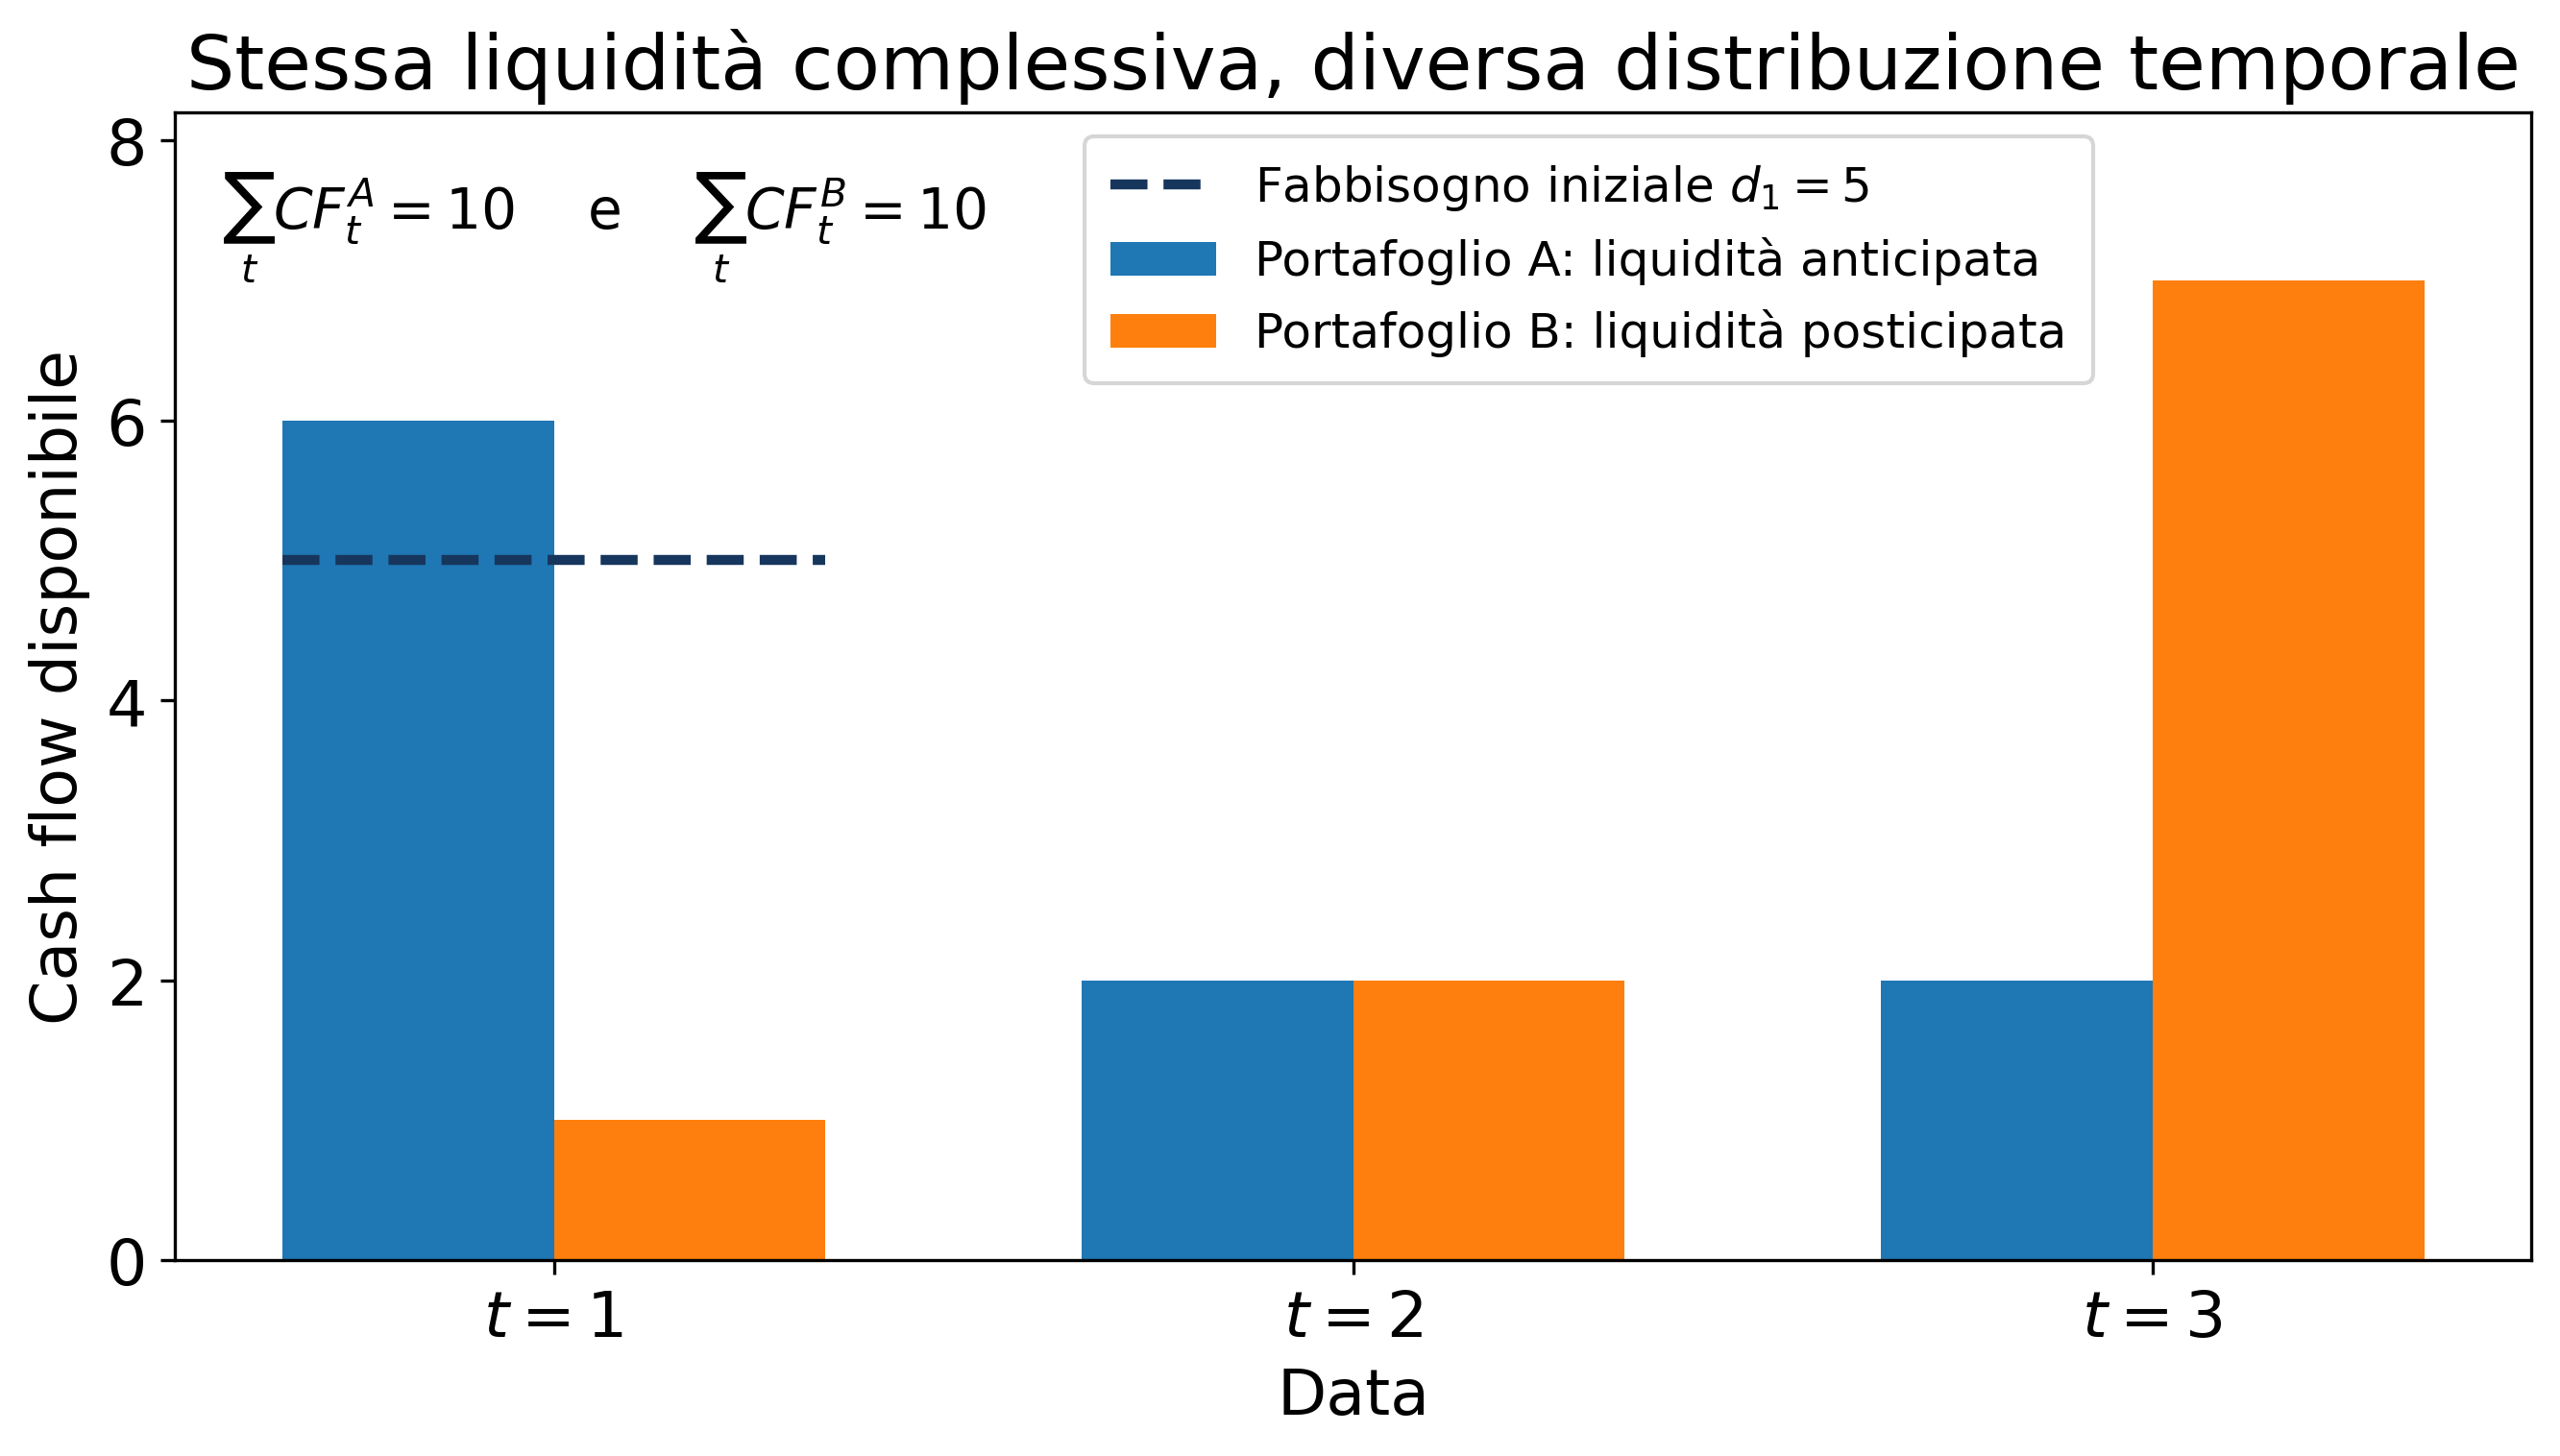
\includegraphics[width=0.90\textwidth]
{../graphics/Cap12_liquidita_aggregata_temporale.png}
\caption{Due portafogli con lo stesso cash flow complessivo ma con diversa
distribuzione temporale. Il portafoglio $A$ produce liquidit\`a in misura
sufficiente a soddisfare il fabbisogno $d_1=5$ alla prima data; il
portafoglio $B$ concentra invece gran parte dei propri flussi alla data
finale.}
\label{fig:cap12-liquidita-aggregata-temporale}
\end{figure}

La Figura~\ref{fig:cap12-liquidita-aggregata-temporale} mostra quindi che la
somma dei cash flow lungo l'intero orizzonte non \`e sufficiente per valutare
la capacit\`a della banca di far fronte ai propri impegni.

La differenza rilevante non riguarda soltanto la quantit\`a complessiva di
liquidit\`a, ma la sua distribuzione nel tempo:

\[
\text{quanto}
\qquad\longrightarrow\qquad
\text{quanto e quando}.
\]

Lo stesso problema si presenta dal lato delle passivit\`a. Una banca non deve
soddisfare un unico fabbisogno aggregato, ma una successione di obblighi,
rimborsi e deflussi collocati in date differenti. La compatibilit\`a tra
attivo e passivo richiede pertanto di confrontare, periodo per periodo, i
flussi prodotti dalle attivit\`a con le risorse richieste dalle passivit\`a.

Introduciamo quindi una sequenza di date

\[
t=0,1,\ldots,T.
\]

Il tempo $t=0$ rappresenta la data nella quale viene scelta la composizione
iniziale del bilancio; le date $t=1,\ldots,T$ rappresentano invece le
scadenze future nelle quali si manifestano cash flow e fabbisogni.

Il problema non consiste pi\`u soltanto nello scegliere una composizione
dell'attivo che soddisfi un requisito complessivo di liquidit\`a. Occorre
scegliere una struttura del bilancio che renda compatibili i flussi generati
dall'attivo con i fabbisogni del passivo lungo l'intero orizzonte temporale.

Il passaggio centrale pu\`o essere sintetizzato come

\[
\boxed{
\text{requisito aggregato di liquidit\`a}
\quad\longrightarrow\quad
\text{bilanci di liquidit\`a alle diverse date}.
}
\]

Questa estensione costituisce il punto di ingresso
nell'Asset--Liability Management deterministico. Il problema resta un
programma lineare: non viene introdotta una nuova classe di ottimizzazione.
Cambiano invece la struttura dei dati e dei vincoli, perch\'e le decisioni
devono ora essere coerenti con una successione di cash flow e fabbisogni
distribuiti nel tempo.

\section{Cash flow degli attivi e fabbisogni alle diverse date}

\label{sec:cap12-cash-flow-fabbisogni}

La sezione precedente ha mostrato che due portafogli con lo stesso cash flow
complessivo possono avere capacit\`a molto diverse di fronteggiare i
fabbisogni della banca. Per rappresentare questa differenza occorre descrivere
separatamente i flussi monetari prodotti alle diverse date.

Consideriamo l'orizzonte discreto

\[
t=0,1,\ldots,T,
\]

e manteniamo il vettore delle decisioni iniziali

\[
x=
\begin{pmatrix}
x_1\\
\vdots\\
x_n
\end{pmatrix},
\]

dove $x_j$ rappresenta l'ammontare destinato alla classe di attivo $j$ al
tempo $0$.

\subsection{Il profilo temporale dei cash flow}

Per ogni attivit\`a $j$ e per ogni data futura $t$, indichiamo con

\[
a_{tj}
\]

il cash flow monetario disponibile alla data $t$ per una unit\`a investita
nell'attivit\`a $j$ al tempo $0$.

L'investimento $x_j$ produce quindi alla data $t$ il flusso

\[
a_{tj}x_j.
\]

Per effetto dell'ipotesi di proporzionalit\`a gi\`a introdotta nel
Capitolo 11, il coefficiente $a_{tj}$ viene trattato come indipendente
dall'ammontare investito. Il cash flow complessivamente prodotto dall'attivo
alla data $t$ \`e pertanto

\[
\sum_{j=1}^{n}a_{tj}x_j.
\]

I coefficienti possono essere raccolti nella matrice dei cash flow

\[
A^{\mathrm{CF}}
=
\begin{pmatrix}
a_{11} & a_{12} & \cdots & a_{1n}\\
a_{21} & a_{22} & \cdots & a_{2n}\\
\vdots & \vdots & \ddots & \vdots\\
a_{T1} & a_{T2} & \cdots & a_{Tn}
\end{pmatrix}.
\]

La matrice $A^{\mathrm{CF}}$ ha $T$ righe e $n$ colonne.

Ogni colonna

\[
\begin{pmatrix}
a_{1j}\\
a_{2j}\\
\vdots\\
a_{Tj}
\end{pmatrix}
\]

descrive il profilo temporale dei cash flow prodotti da una unit\`a della
classe di attivo $j$.

Ogni riga

\[
(a_{t1},\ldots,a_{tn})
\]

descrive invece i cash flow unitari prodotti alla data $t$ dalle diverse
classi di attivo.

Questa organizzazione mantiene la logica matriciale introdotta nel
Capitolo 11. Una colonna continua a descrivere come una variabile decisionale
contribuisce ai diversi requisiti del modello; nel problema multiperiodale,
tali contributi sono ora distinti anche in base alla data nella quale si
manifestano.

\subsection{Il profilo dei fabbisogni}

Dal lato delle passivit\`a, indichiamo con

\[
d_t\geq0
\]

il fabbisogno monetario che deve essere soddisfatto alla data $t$.

La quantit\`a $d_t$ rappresenta l'ammontare di risorse che la banca deve
rendere disponibile in quella data. A seconda della specificazione del
modello, esso pu\`o comprendere rimborsi di passivit\`a, pagamenti
contrattuali, deflussi della raccolta o altri impieghi di liquidit\`a.

Nel modello deterministico sviluppato in questo capitolo, i valori

\[
d_1,d_2,\ldots,d_T
\]

sono trattati come dati noti prima della soluzione del problema e vengono
raccolti nel vettore

\[
d=
\begin{pmatrix}
d_1\\
d_2\\
\vdots\\
d_T
\end{pmatrix}.
\]

La natura deterministica di $d_t$ non implica che i futuri deflussi siano
certi nella realt\`a. Significa che il modello analizza le conseguenze di uno
specifico profilo di fabbisogni assunto come dato nella formulazione
considerata.

Pi\`u avanti il modo in cui tali fabbisogni vengono determinati sar\`a
collegato in modo esplicito alle condizioni economico-finanziarie e alla
situazione patrimoniale della banca. Per il momento, tuttavia, interessa
isolare il problema fondamentale del coordinamento temporale tra risorse
disponibili e risorse richieste.

\begin{figure}[htbp]
\centering
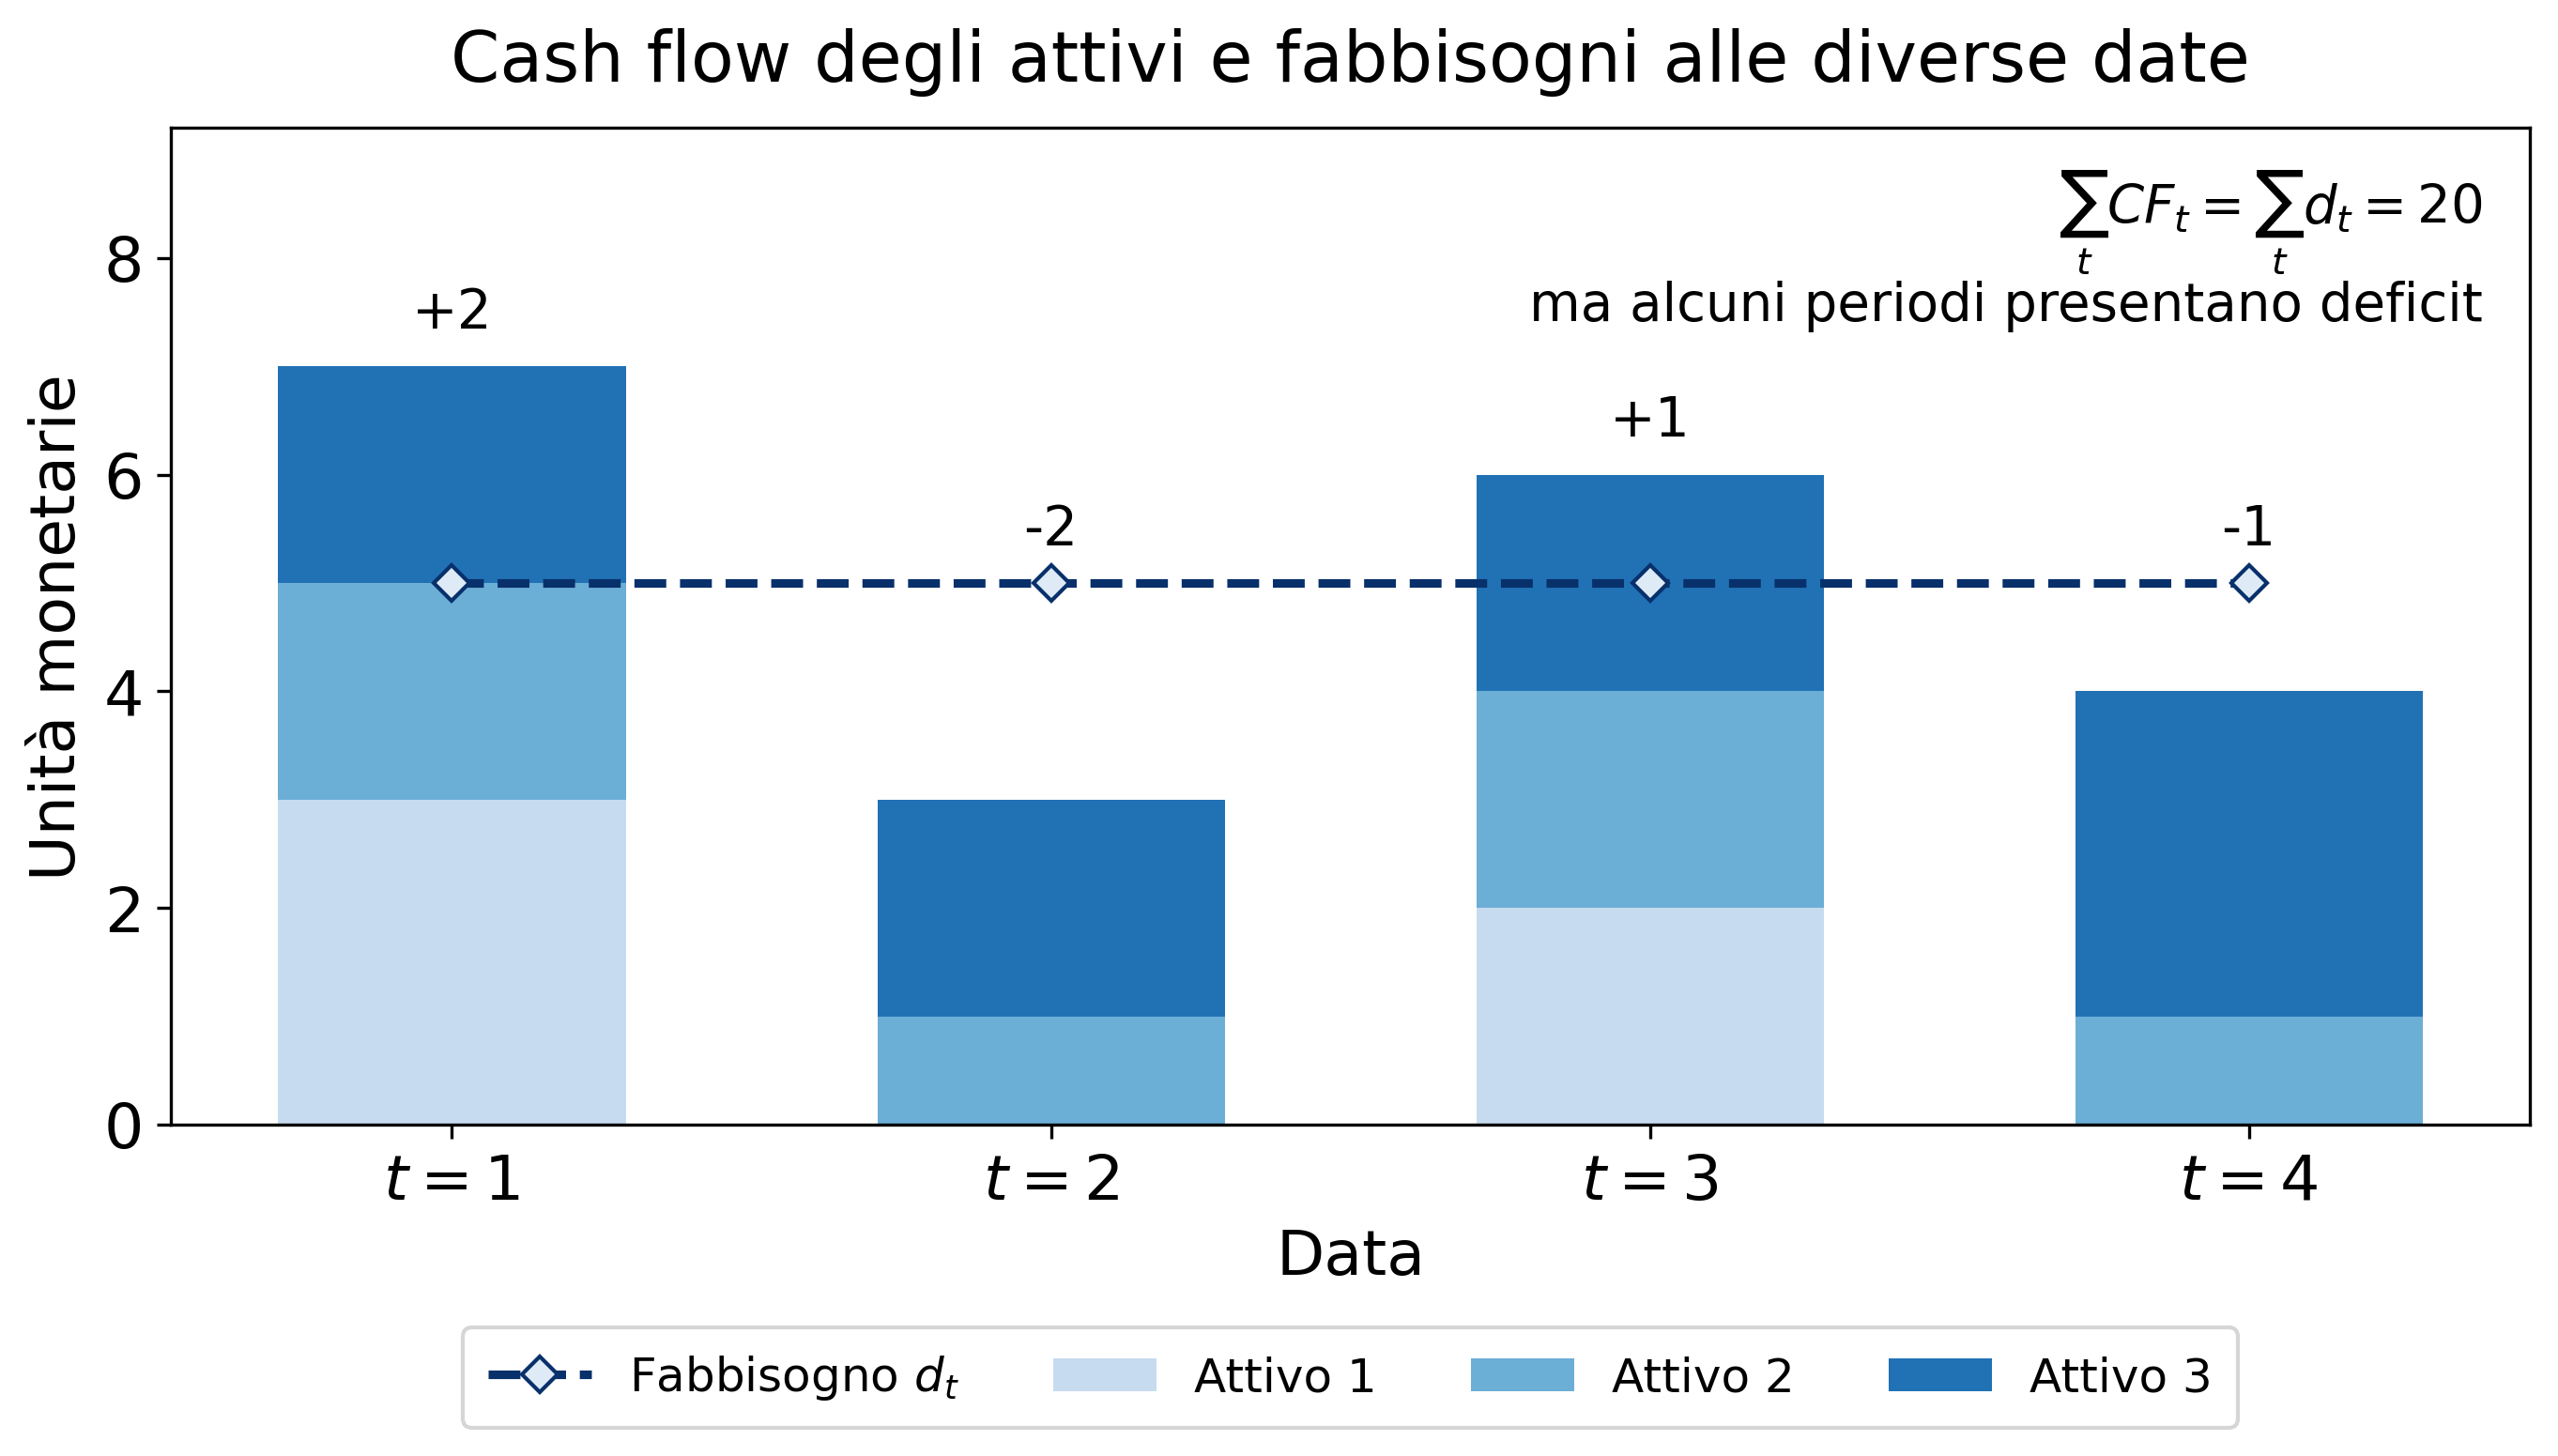
\includegraphics[width=0.92\textwidth]
{../graphics/Cap12_cashflow_attivi_fabbisogni.png}
\caption{Cash flow prodotti dalle diverse classi di attivo e fabbisogni
alle quattro date. Pur coincidendo i cash flow complessivi e i fabbisogni
complessivi sull'intero orizzonte, il profilo temporale presenta surplus
alle date $t=1$ e $t=3$ e deficit alle date $t=2$ e $t=4$.}
\label{fig:cap12-cashflow-fabbisogni}
\end{figure}

La Figura~\ref{fig:cap12-cashflow-fabbisogni} mostra perch\'e il confronto
aggregato non \`e sufficiente. Sull'intero orizzonte le risorse prodotte
dagli attivi coincidono con i fabbisogni:

\[
\sum_{t=1}^{T}CF_t
=
\sum_{t=1}^{T}d_t.
\]

Ci\`o non impedisce tuttavia la presenza di deficit in singole date.
L'Asset--Liability Management deve quindi verificare non soltanto
l'equilibrio complessivo delle risorse, ma la loro disponibilit\`a nel
momento in cui i pagamenti devono essere effettuati.

\subsection{Una prima formulazione: cash-flow matching per data}

Una prima formulazione consiste nel richiedere che, a ciascuna data, i cash
flow prodotti dagli attivi siano almeno sufficienti a coprire il fabbisogno
corrispondente:

\[
\sum_{j=1}^{n}a_{tj}x_j
\geq
d_t,
\qquad
t=1,\ldots,T.
\]

In forma matriciale,

\[
A^{\mathrm{CF}}x
\geq
d.
\]

Il singolo requisito aggregato di liquidit\`a del Capitolo 11 viene quindi
sostituito da $T$ requisiti distinti. La dimensione temporale non viene pi\`u
compressa in un unico coefficiente: per ciascuna data il modello confronta le
risorse monetarie prodotte dall'attivo con il corrispondente fabbisogno.

Questa formulazione rappresenta un primo modello di \emph{cash-flow
matching}. Una composizione dell'attivo \`e ammissibile soltanto se i cash
flow disponibili risultano sufficienti in tutte le date considerate.

Il passaggio dal requisito aggregato

\[
\sum_{j=1}^{n}q_jx_j
\geq
Q_{\min}
\]

ai vincoli

\[
\sum_{j=1}^{n}a_{tj}x_j
\geq
d_t,
\qquad
t=1,\ldots,T,
\]

rende esplicita una differenza fondamentale. Nel primo caso la liquidit\`a
viene misurata come caratteristica complessiva della composizione
dell'attivo; nel secondo viene confrontata con fabbisogni che possiedono una
scadenza precisa.

\subsection{Il limite del matching separato per data}

La formulazione precedente introduce correttamente il tempo, ma considera
ancora ogni data come se fosse indipendente dalle altre.

Supponiamo che, alla data $t$, il portafoglio produca un cash flow superiore
al fabbisogno:

\[
\sum_{j=1}^{n}a_{tj}x_j
>
d_t.
\]

La differenza

\[
\sum_{j=1}^{n}a_{tj}x_j-d_t
\]

rappresenta una disponibilit\`a monetaria residua dopo avere soddisfatto il
fabbisogno della data $t$.

Nei vincoli di cash-flow matching appena formulati, tuttavia, questa
eccedenza non compare nel periodo successivo. Le risorse disponibili alla
data $t$ che non vengono utilizzate scompaiono dal modello e non possono
contribuire alla copertura del fabbisogno alla data $t+1$.

Si tratta di una limitazione economicamente rilevante. Una banca pu\`o
conservare una parte della liquidit\`a disponibile oppure reinvestirla in una
forma compatibile con l'orizzonte successivo. La posizione di liquidit\`a di
una data dipende quindi anche da quanto \`e accaduto nelle date precedenti.

Il problema ALM non pu\`o essere descritto come una semplice successione di
$T$ vincoli indipendenti. Occorre introdurre una variabile che rappresenti la
liquidit\`a residua trasferita da un periodo al successivo.

Il passaggio successivo \`e quindi

\[
\boxed{
\text{cash-flow matching per data}
\quad\longrightarrow\quad
\text{bilanci di liquidit\`a collegati nel tempo}.
}
\]

L'introduzione di questa variabile render\`a esplicita la dipendenza tra il
vincolo relativo alla data $t$ e quello relativo alla data $t+1$ e
costituir\`a il primo vero elemento intertemporale del modello ALM.

\section{Liquidit\`a residua e bilanci intertemporali}

\label{sec:cap12-bilanci-intertemporali}

Il cash-flow matching introdotto nella
Sezione~\ref{sec:cap12-cash-flow-fabbisogni} confronta, per ogni data,
i flussi prodotti dall'attivo con il corrispondente fabbisogno:

\[
\sum_{j=1}^{n}a_{tj}x_j
\geq
d_t,
\qquad
t=1,\ldots,T.
\]

Questa formulazione riconosce che la liquidit\`a deve essere disponibile
nella data in cui viene richiesta, ma non descrive ancora che cosa accade
quando i cash flow prodotti in un periodo superano il fabbisogno dello stesso
periodo.

In una gestione intertemporale, l'eccedenza non scompare. Pu\`o essere
conservata e utilizzata nelle date successive. Per rappresentare questo
meccanismo introduciamo una nuova variabile decisionale.

\begin{definition}[Giacenza di liquidit\`a]

Per ogni data $t=1,\ldots,T$, indichiamo con

\[
g_t\geq0
\]

la liquidit\`a che rimane disponibile immediatamente dopo avere soddisfatto
il fabbisogno $d_t$.

\end{definition}

La variabile $g_t$ \`e quindi uno \emph{stock}, misurato in unit\`a
monetarie. Non rappresenta un nuovo cash flow prodotto dall'attivo, ma la
parte delle risorse disponibili alla data $t$ che non viene utilizzata e
viene trasferita al periodo successivo.

\subsection{Il primo bilancio temporale}

Consideriamo inizialmente la prima data, $t=1$.

I cash flow prodotti dall'attivo sono

\[
\sum_{j=1}^{n}a_{1j}x_j.
\]

Queste risorse devono essere utilizzate per soddisfare il fabbisogno $d_1$;
l'eventuale eccedenza costituisce la giacenza $g_1$.

Il bilancio monetario alla prima data \`e quindi

\[
\sum_{j=1}^{n}a_{1j}x_j
=
d_1+g_1.
\]

La relazione \`e un'uguaglianza, non una disuguaglianza. Tutte le risorse
monetarie disponibili alla data $1$ devono avere una destinazione: una parte
viene utilizzata per soddisfare il fabbisogno, la parte restante viene
conservata come liquidit\`a.

Equivalentemente,

\[
g_1
=
\sum_{j=1}^{n}a_{1j}x_j-d_1.
\]

La condizione

\[
g_1\geq0
\]

garantisce che il fabbisogno della prima data possa essere interamente
soddisfatto.

\subsection{Il collegamento con la data successiva}

Alla data $t=2$ la banca dispone di due fonti di liquidit\`a:

\begin{itemize}

\item i nuovi cash flow prodotti dagli attivi,

\[
\sum_{j=1}^{n}a_{2j}x_j;
\]

\item la giacenza $g_1$ trasferita dalla data precedente.

\end{itemize}

Se, in una prima formulazione, assumiamo che la liquidit\`a trasferita non
produca rendimento, il bilancio alla seconda data diventa

\[
\sum_{j=1}^{n}a_{2j}x_j
+
g_1
=
d_2+g_2.
\]

Pi\`u in generale, per

\[
t=2,\ldots,T,
\]

si ottiene

\[
\sum_{j=1}^{n}a_{tj}x_j
+
g_{t-1}
=
d_t+g_t.
\]

Il sistema completo dei bilanci temporali \`e pertanto

\[
\begin{array}{rcl}
\displaystyle
\sum_{j=1}^{n}a_{1j}x_j
-
g_1
&=&
d_1,
\\[8pt]
\displaystyle
\sum_{j=1}^{n}a_{2j}x_j
+
g_1-g_2
&=&
d_2,
\\
&\vdots&
\\
\displaystyle
\sum_{j=1}^{n}a_{Tj}x_j
+
g_{T-1}-g_T
&=&
d_T.
\end{array}
\]

La differenza rispetto al cash-flow matching separato per data \`e
fondamentale. La variabile $g_t$ compare contemporaneamente nel bilancio
della data $t$ e in quello della data $t+1$.

Il vincolo relativo a una data non pu\`o quindi pi\`u essere interpretato
isolatamente:

\[
\boxed{
g_t
\text{ collega il bilancio della data }t
\text{ al bilancio della data }t+1.
}
\]

Questa \`e la struttura intertemporale essenziale del modello.

\subsection{La liquidit\`a come variabile di stato}

La giacenza $g_t$ possiede una funzione diversa dalle variabili iniziali
$x_j$.

Le quantit\`a

\[
x_1,\ldots,x_n
\]

determinano la composizione dell'attivo \textbf{scelta} al tempo $0$.

La quantit\`a

\[
g_t
\]

descrive invece la posizione di liquidit\`a con la quale la banca conclude la
data $t$ e affronta la data successiva.

In questo senso, $g_t$ pu\`o essere interpretata come una semplice
\emph{variabile di stato}: sintetizza una conseguenza delle decisioni e dei
cash flow passati che diventa rilevante per i vincoli futuri.

Dal bilancio temporale segue infatti la relazione ricorsiva

\[
g_t
=
g_{t-1}
+
\sum_{j=1}^{n}a_{tj}x_j
-
d_t,
\qquad
t=1,\ldots,T,
\]

ponendo per il momento

\[
g_0=0.
\]

La liquidit\`a disponibile alla fine di ogni data dipende quindi dalla
liquidit\`a ereditata dal periodo precedente, dai nuovi flussi prodotti
dall'attivo e dal fabbisogno corrente.

Questa rappresentazione rende esplicito un principio centrale
dell'Asset--Liability Management:

\[
\boxed{
\begin{array}{c}
\text{la posizione finanziaria a una data dipende anche}\\
\text{dalle decisioni e dai saldi accumulati nelle date precedenti}
\end{array}
}
\]

\subsection{Il rendimento della liquidit\`a trasferita}

L'ipotesi secondo cui la liquidit\`a trasferita da una data alla successiva
mantenga invariato il proprio valore \`e utile per isolare la struttura dei
bilanci, ma pu\`o essere raffinata.

Supponiamo che la giacenza disponibile dopo la data $t-1$ possa essere
impiegata fino alla data $t$ a un tasso deterministico $r_{t-1}$.

Una unit\`a monetaria detenuta alla fine della data $t-1$ diventa quindi

\[
1+r_{t-1}
\]

unit\`a alla data $t$.

Per $t=2,\ldots,T$, il bilancio diventa

\[
\sum_{j=1}^{n}a_{tj}x_j
+
(1+r_{t-1})g_{t-1}
=
d_t+g_t.
\]

Per la prima data resta

\[
\sum_{j=1}^{n}a_{1j}x_j
=
d_1+g_1,
\]

se si assume che non esista una giacenza iniziale separata dalla composizione
$x$ scelta al tempo $0$.

Il sistema pu\`o quindi essere scritto come

\[
\begin{array}{rcl}
\displaystyle
\sum_{j=1}^{n}a_{1j}x_j-g_1
&=&
d_1,
\\[8pt]
\displaystyle
\sum_{j=1}^{n}a_{2j}x_j
+
(1+r_1)g_1-g_2
&=&
d_2,
\\
&\vdots&
\\
\displaystyle
\sum_{j=1}^{n}a_{Tj}x_j
+
(1+r_{T-1})g_{T-1}-g_T
&=&
d_T.
\end{array}
\]

Il coefficiente $1+r_{t-1}$ non modifica la natura lineare del modello,
poich\'e il tasso $r_{t-1}$ \`e trattato come un dato deterministico.

\subsection{Condizione finale}

La variabile $g_T$ rappresenta la liquidit\`a residua alla fine
dell'orizzonte considerato. Il suo trattamento dipende dalla funzione del
modello.

Se l'orizzonte termina quando tutti gli obblighi rilevanti sono stati
soddisfatti e non si attribuisce valore alla liquidit\`a residua, pu\`o essere
imposta la condizione

\[
g_T=0.
\]

Se invece la liquidit\`a finale rappresenta una risorsa economicamente utile
oltre l'orizzonte del modello, essa non deve essere forzata a zero: dovr\`a
essere mantenuta come variabile oppure valorizzata nella funzione obiettivo.

La condizione terminale non \`e quindi un dettaglio tecnico. Stabilisce che
cosa il modello considera economicamente rilevante al termine
dell'orizzonte.

\subsection{Dal matching al bilancio dinamico}

Il passaggio compiuto in questa sezione pu\`o essere riassunto confrontando le
due formulazioni.

Nel cash-flow matching separato per data:

\[
\sum_{j=1}^{n}a_{tj}x_j
\geq
d_t.
\]

Nel modello con trasferimento della liquidit\`a:

\[
\sum_{j=1}^{n}a_{tj}x_j
+
(1+r_{t-1})g_{t-1}
=
d_t+g_t.
\]

Nel primo caso ciascuna data costituisce un confronto autonomo tra flussi e
fabbisogni. Nel secondo, il saldo di un periodo diventa una risorsa del
periodo successivo.

La programmazione rimane lineare, ma la struttura economica del problema
cambia profondamente: il modello non confronta pi\`u soltanto attivit\`a e
passivit\`a alle singole date, bens\`i descrive l'evoluzione nel tempo della
posizione di liquidit\`a della banca.

Questo collegamento prepara il passo successivo. La liquidit\`a accumulata
internamente non \`e infatti l'unico strumento con cui una banca pu\`o
fronteggiare un fabbisogno temporaneo. Quando i cash flow dell'attivo e la
giacenza disponibile non sono sufficienti, la banca pu\`o ricorrere a
funding esterno. Tale scelta produce liquidit\`a nella data corrente, ma
genera contemporaneamente un obbligo di rimborso futuro.

\section{Funding esterno e obblighi di rimborso}

\label{sec:cap12-funding}

I bilanci intertemporali introdotti nella
Sezione~\ref{sec:cap12-bilanci-intertemporali} assumono che la banca possa
soddisfare i propri fabbisogni utilizzando esclusivamente i cash flow prodotti
dall'attivo e la liquidit\`a accumulata nelle date precedenti.

Questa rappresentazione mette in evidenza il collegamento temporale tra le
diverse date, ma trascura una possibilit\`a importante. Se le risorse interne
non sono sufficienti a soddisfare un fabbisogno corrente, la banca pu\`o
ricorrere a una fonte esterna di funding.

Il funding modifica la disponibilit\`a di liquidit\`a nella data in cui viene
raccolto, ma non costituisce una risorsa gratuita. Le somme ottenute devono
essere rimborsate in una data successiva insieme al relativo costo
finanziario.

\subsection{Una fonte di funding a un periodo}

Per mantenere leggibile la struttura del modello, consideriamo una sola forma
stilizzata di funding con durata pari a un periodo.

Per

\[
t=1,\ldots,T-1,
\]

indichiamo con

\[
u_t\geq0
\]

l'ammontare di funding raccolto alla data $t$.

La quantit\`a $u_t$ \`e immediatamente disponibile e pu\`o quindi essere
utilizzata per soddisfare il fabbisogno della stessa data.

Supponiamo che il funding raccolto alla data $t$ debba essere rimborsato alla
data $t+1$ a un tasso deterministico $\rho_t$. L'obbligo di rimborso generato
da $u_t$ \`e pertanto

\[
(1+\rho_t)u_t.
\]

La sequenza economica \`e quindi

\[
\boxed{
\begin{array}{c}
\text{funding raccolto alla data }t:\quad u_t\\[3pt]
\downarrow\\[3pt]
\text{liquidit\`a disponibile alla data }t\\[3pt]
\downarrow\\[3pt]
\text{rimborso alla data }t+1:\quad (1+\rho_t)u_t
\end{array}
}
\]

Il funding trasferisce quindi risorse dalla data futura alla data corrente:
aumenta la liquidit\`a disponibile oggi, ma riduce quella disponibile domani.

\subsection{Il bilancio alla prima data}

Alla data $t=1$ la banca dispone dei cash flow prodotti dagli attivi,

\[
\sum_{j=1}^{n}a_{1j}x_j,
\]

e pu\`o inoltre raccogliere funding per un ammontare $u_1$.

Le risorse vengono utilizzate per soddisfare il fabbisogno $d_1$ e
l'eventuale eccedenza viene mantenuta come giacenza $g_1$.

Il bilancio diventa quindi

\[
\sum_{j=1}^{n}a_{1j}x_j
+
u_1
=
d_1+g_1.
\]

Rispetto alla formulazione della sezione precedente, il termine $u_1$
costituisce una nuova fonte di liquidit\`a.

Il suo utilizzo produce tuttavia un effetto sul periodo successivo.

\subsection{Il bilancio nelle date intermedie}

Consideriamo una generica data

\[
t=2,\ldots,T-1.
\]

Le risorse disponibili sono ora costituite da tre componenti:

\begin{itemize}

\item i cash flow prodotti dagli attivi,

\[
\sum_{j=1}^{n}a_{tj}x_j;
\]

\item la giacenza proveniente dalla data precedente, capitalizzata al tasso
$r_{t-1}$,

\[
(1+r_{t-1})g_{t-1};
\]

\item il nuovo funding raccolto alla data corrente,

\[
u_t.
\]

\end{itemize}

A queste risorse si contrappongono tre utilizzi:

\begin{itemize}

\item il fabbisogno corrente $d_t$;

\item il rimborso del funding raccolto alla data precedente,

\[
(1+\rho_{t-1})u_{t-1};
\]

\item la nuova giacenza di liquidit\`a $g_t$.

\end{itemize}

Il bilancio intertemporale completo \`e quindi

\[
\sum_{j=1}^{n}a_{tj}x_j
+
(1+r_{t-1})g_{t-1}
+
u_t
=
d_t
+
(1+\rho_{t-1})u_{t-1}
+
g_t.
\]

La stessa variabile $u_t$ svolge quindi due ruoli in date consecutive:

\[
u_t
\]

\`e una risorsa nel bilancio della data $t$, mentre

\[
(1+\rho_t)u_t
\]

diventa un utilizzo nel bilancio della data $t+1$.

Il funding introduce cos\`i un secondo collegamento intertemporale, accanto a
quello gi\`a prodotto dalla giacenza $g_t$.

\begin{figure}[htbp]
\centering
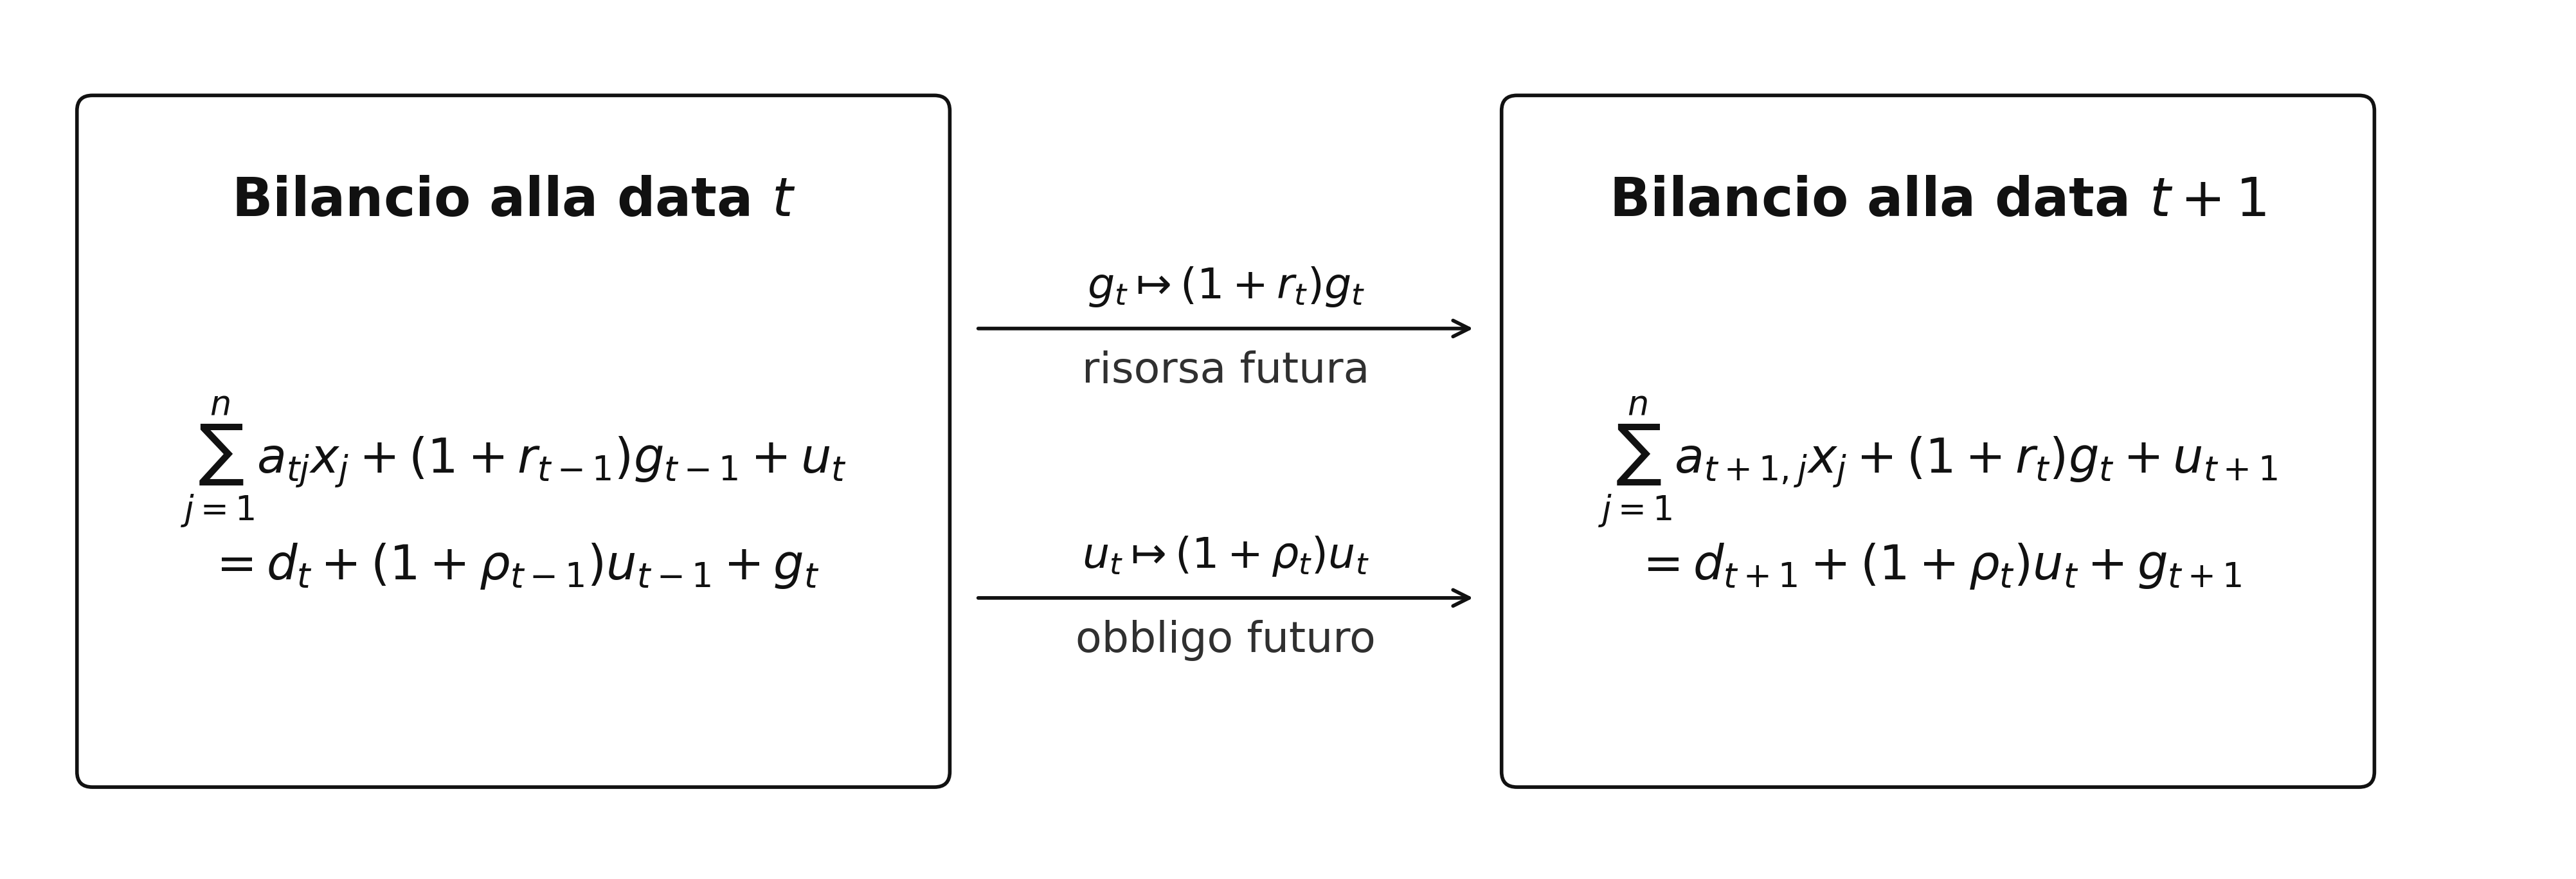
\includegraphics[width=0.96\textwidth]
{../graphics/Cap12_bilancio_intertemporale.png}
\caption{Collegamento tra due bilanci di liquidit\`a consecutivi. La
giacenza $g_t$ costituisce una risorsa disponibile alla data successiva,
mentre il funding $u_t$ raccolto alla data corrente genera un obbligo di
rimborso pari a $(1+\rho_t)u_t$ alla data successiva.}
\label{fig:cap12-bilancio-intertemporale}
\end{figure}

La Figura~\ref{fig:cap12-bilancio-intertemporale} rende visibili i due
collegamenti fondamentali tra date consecutive. La giacenza trasferisce
risorse verso il futuro; il funding trasferisce invece risorse dal futuro
al presente e genera per questo un successivo obbligo di rimborso.

Le due variabili hanno quindi effetti temporali opposti:

\[
g_t
\quad\text{accumula una risorsa per il periodo successivo},
\]

mentre

\[
u_t
\quad\text{anticipa una risorsa creando un'obbligazione futura}.
\]

La struttura intertemporale del modello nasce precisamente dalla presenza
simultanea di questi collegamenti.

\subsection{Il bilancio alla data finale}

Alla data finale $T$ non introduciamo nuovo funding. Questa scelta garantisce
che ogni posizione di funding aperta all'interno dell'orizzonte venga anche
rimborsata entro l'orizzonte stesso.

Il bilancio finale \`e pertanto

\[
\sum_{j=1}^{n}a_{Tj}x_j
+
(1+r_{T-1})g_{T-1}
=
d_T
+
(1+\rho_{T-1})u_{T-1}
+
g_T.
\]

Il sistema completo pu\`o quindi essere scritto come

\[
\begin{array}{rcl}
\displaystyle
\sum_{j=1}^{n}a_{1j}x_j+u_1-g_1
&=&
d_1,
\\[8pt]
\displaystyle
\sum_{j=1}^{n}a_{tj}x_j
+
(1+r_{t-1})g_{t-1}
+
u_t
-
(1+\rho_{t-1})u_{t-1}
-
g_t
&=&
d_t,
\\
&&
t=2,\ldots,T-1,
\\[8pt]
\displaystyle
\sum_{j=1}^{n}a_{Tj}x_j
+
(1+r_{T-1})g_{T-1}
-
(1+\rho_{T-1})u_{T-1}
-
g_T
&=&
d_T.
\end{array}
\]

Le condizioni di non negativit\`a sono

\[
g_t\geq0,
\qquad
t=1,\ldots,T,
\]

e

\[
u_t\geq0,
\qquad
t=1,\ldots,T-1.
\]

\subsection{Limiti alla disponibilit\`a di funding}

La possibilit\`a di raccogliere funding non pu\`o essere considerata
illimitata.

Introduciamo pertanto, per ogni data,

\[
\bar{u}_t\geq0,
\]

che rappresenta l'ammontare massimo di funding accessibile alla banca.

Il vincolo

\[
0\leq u_t\leq\bar{u}_t,
\qquad
t=1,\ldots,T-1,
\]

pu\`o riflettere limiti contrattuali, capacit\`a di accesso al mercato,
disponibilit\`a di linee di credito o altri vincoli sulla raccolta
incrementale.

Il parametro $\bar{u}_t$ ha un significato diverso da $u_t$:

\[
u_t
=
\text{decisione di funding},
\]

mentre

\[
\bar{u}_t
=
\text{massima capacit\`a di funding disponibile}.
\]

La banca decide quindi quanto funding utilizzare all'interno di una
capacit\`a data.

\subsection{Costo del funding e assenza di arbitraggio artificiale}

Il tasso $\rho_t$ rappresenta il costo complessivo della fonte di funding
utilizzata tra le date $t$ e $t+1$.

Nello stesso intervallo, la giacenza di liquidit\`a produce il rendimento
$r_t$.

Per evitare che il modello trovi conveniente raccogliere funding unicamente
per investirlo nella giacenza di liquidit\`a, \`e naturale assumere

\[
\rho_t\geq r_t.
\]

In una rappresentazione bancaria realistica ci si attende normalmente

\[
\rho_t>r_t,
\]

poich\'e la raccolta esterna incorpora un costo superiore al rendimento di una
posizione liquida priva di rischio comparabile.

La differenza

\[
\rho_t-r_t
\]

rappresenta quindi, in forma stilizzata, il costo aggiuntivo associato
all'accesso al funding.

Questa condizione non \`e necessaria per la linearit\`a matematica del
problema, ma evita un comportamento economicamente artificiale del modello.

\subsection{Funding e gestione della liquidit\`a}

L'introduzione di $u_t$ modifica il significato del problema ALM.

Senza funding, un'insufficienza dei cash flow e della liquidit\`a accumulata
rende il piano non ammissibile.

Con il funding, la banca dispone di una seconda possibilit\`a:

\[
\text{deficit corrente}
\quad\longrightarrow\quad
\text{funding oggi}
\quad\longrightarrow\quad
\text{obbligo di rimborso domani}.
\]

Il funding non elimina quindi il problema della liquidit\`a. Ne modifica la
distribuzione temporale.

Una scelta di funding che risolve un deficit alla data $t$ pu\`o infatti
rendere pi\`u difficile soddisfare il bilancio alla data $t+1$, a causa del
rimborso

\[
(1+\rho_t)u_t.
\]

La decisione non pu\`o pertanto essere valutata considerando esclusivamente il
periodo corrente.

Il modello comincia cos\`i a rappresentare il nucleo dell'Asset--Liability
Management:

\[
\boxed{
\begin{array}{c}
\text{le risorse disponibili oggi dipendono dalle decisioni passate,}\\
\text{mentre le decisioni assunte oggi modificano i fabbisogni futuri.}
\end{array}
}
\]

La struttura resta interamente lineare. I coefficienti $a_{tj}$, $d_t$,
$r_t$, $\rho_t$ e $\bar{u}_t$ sono, in questa fase, dati deterministici;
$x_j$, $g_t$ e $u_t$ sono invece le variabili attraverso le quali il modello
descrive la composizione dell'attivo e la gestione intertemporale della
liquidit\`a.

La sezione successiva preciser\`a come tali coefficienti possano essere
ricondotti a un ambiente economico-finanziario deterministico e come il
modello ALM possa essere collegato in modo coerente al caso bancario
sviluppato nel Capitolo 11.

\section{L'ambiente economico-finanziario deterministico}

\label{sec:cap12-ambiente-deterministico}

Le sezioni precedenti hanno costruito la struttura intertemporale del modello
ALM. I cash flow degli attivi, la giacenza di liquidit\`a e il funding
collegano le diverse date attraverso i bilanci

\[
\sum_{j=1}^{n}a_{tj}x_j
+
(1+r_{t-1})g_{t-1}
+
u_t
=
d_t
+
(1+\rho_{t-1})u_{t-1}
+
g_t.
\]

Finora i coefficienti

\[
a_{tj},\qquad r_t,\qquad \rho_t,\qquad \bar{u}_t
\]

sono stati trattati semplicemente come dati del modello. In un problema
bancario, tuttavia, tali coefficienti riflettono le condizioni
economico-finanziarie nelle quali la banca opera.

Per rendere esplicito questo collegamento introduciamo, per ogni data
$t=0,1,\ldots,T$, il vettore

\[
\bar{Z}_t
=
\left(
\bar{R}_t,\bar{C}_t,\bar{F}_t
\right).
\]

La barra indica che, nel presente capitolo, l'intera traiettoria

\[
\bar{Z}_0,\bar{Z}_1,\ldots,\bar{Z}_T
\]

\`e considerata nota al momento della formulazione del problema.

Il modello \`e quindi deterministico, ma i valori dei fattori possono variare
nel tempo:

\[
\bar{Z}_t
\neq
\bar{Z}_{t+1}.
\]

La caratteristica deterministica riguarda la conoscenza della traiettoria,
non la sua costanza.

\subsection{Tre dimensioni dell'ambiente finanziario}

Le tre componenti di $\bar{Z}_t$ hanno funzioni economiche distinte.

Il fattore

\[
\bar{R}_t
\]

rappresenta il livello dei tassi privi di rischio rilevante nell'intervallo
considerato. Esso pu\`o essere interpretato come il \emph{prezzo del tempo}:
determina il rendimento delle disponibilit\`a liquide e contribuisce alla
valutazione dei flussi monetari distribuiti nel tempo.

Il fattore

\[
\bar{C}_t
\]

rappresenta il livello dello spread di credito osservato sul mercato. Esso
misura il premio richiesto per detenere esposizioni soggette a rischio di
credito e pu\`o essere interpretato come il \emph{prezzo del rischio di
credito}.

Il fattore

\[
\bar{F}_t
\]

rappresenta invece lo spread o la tensione associata al funding della banca.
Esso misura quanto l'accesso alla raccolta esterna sia costoso o difficile
rispetto a una fonte priva di rischio comparabile e pu\`o essere interpretato
come il \emph{prezzo della scarsit\`a di funding}.

La distinzione pu\`o essere sintetizzata come

\[
\boxed{
\begin{array}{c}
\bar{R}_t:\ \text{prezzo del tempo},\\[3pt]
\bar{C}_t:\ \text{prezzo del rischio di credito},\\[3pt]
\bar{F}_t:\ \text{prezzo della scarsit\`a di funding}.
\end{array}
}
\]

I tre fattori descrivono l'ambiente esterno nel quale la banca opera. Non
dipendono dalle decisioni $x_j$, $g_t$ o $u_t$ assunte nel modello.

\subsection{Dal livello dei tassi al rendimento della liquidit\`a}

Nella Sezione~\ref{sec:cap12-bilanci-intertemporali} il parametro $r_t$
rappresenta il rendimento ottenibile mantenendo una giacenza di liquidit\`a
tra le date $t$ e $t+1$.

Il suo valore pu\`o essere ricondotto al livello del tasso privo di rischio:

\[
r_t
=
r(\bar{R}_t).
\]

Nella rappresentazione pi\`u semplice, se $\bar{R}_t$ indica direttamente il
tasso applicabile alla giacenza nell'intervallo considerato, si pu\`o porre

\[
r_t=\bar{R}_t.
\]

Il bilancio utilizza quindi

\[
(1+\bar{R}_t)g_t
\]

come ammontare disponibile alla data successiva.

La relazione non deve essere interpretata come una legge generale di mercato.
Essa costituisce una specificazione coerente con un modello nel quale la
liquidit\`a residua viene investita per un periodo in una forma a rischio
trascurabile.

\subsection{Il costo del funding}

Il tasso $\rho_t$ introdotto nella
Sezione~\ref{sec:cap12-funding} rappresenta invece il costo del funding
raccolto alla data $t$ e rimborsato alla data $t+1$.

Il suo valore dipende sia dal livello generale dei tassi sia dalle condizioni
specifiche di funding della banca. Una rappresentazione naturale \`e

\[
\rho_t
=
\rho(\bar{R}_t,\bar{F}_t).
\]

Se $\bar{F}_t$ viene misurato direttamente come spread sul tasso privo di
rischio, una specificazione particolarmente semplice \`e

\[
\rho_t
=
\bar{R}_t+\bar{F}_t.
\]

Il rimborso del funding diventa quindi

\[
\left(
1+\bar{R}_t+\bar{F}_t
\right)u_t.
\]

Questa rappresentazione rende esplicita la differenza tra il rendimento della
liquidit\`a e il costo della raccolta esterna. Se

\[
\bar{F}_t>0,
\]

allora

\[
\rho_t>r_t,
\]

coerentemente con l'ipotesi introdotta nella sezione precedente.

Il funding \`e quindi tanto pi\`u costoso quanto maggiore \`e la tensione
associata alla raccolta della banca.

\subsection{Disponibilit\`a di funding}

Le condizioni di funding possono incidere non soltanto sul costo della
raccolta, ma anche sull'ammontare massimo accessibile.

Il parametro

\[
\bar{u}_t
\]

rappresenta la capacit\`a massima di funding disponibile alla data $t$.

In forma generale si pu\`o scrivere

\[
\bar{u}_t
=
\bar{u}(\bar{F}_t).
\]

In condizioni di funding favorevoli la banca pu\`o disporre di una maggiore
capacit\`a di raccolta; in condizioni di stress tale capacit\`a pu\`o
ridursi.

Non \`e necessario specificare in questa fase una particolare forma
funzionale. Nel problema deterministico, una volta fissata la traiettoria
$\bar{F}_t$, anche

\[
\bar{u}_1,\ldots,\bar{u}_{T-1}
\]

sono coefficienti noti.

Il vincolo

\[
0\leq u_t\leq\bar{u}_t
\]

rimane pertanto lineare.

\subsection{Il ruolo dello spread di credito}

Il fattore $\bar{C}_t$ richiede una precisazione particolare.

Se un'attivit\`a produce cash flow contrattuali certi e viene mantenuta fino
alla scadenza, una variazione dello spread di credito di mercato non modifica
automaticamente tali cash flow.

Non sarebbe quindi corretto introdurre $\bar{C}_t$ nei coefficienti
$a_{tj}$ per il solo fatto che il modello contiene un fattore di credito.

Il fattore $\bar{C}_t$ diventa invece rilevante quando i flussi disponibili
per l'ALM dipendono dalla qualit\`a creditizia o dal valore economico delle
attivit\`a. Ci\`o pu\`o accadere, per esempio, quando il modello considera:

\begin{itemize}

\item cash flow corretti per perdite creditizie;

\item valori di realizzo di titoli o prestiti;

\item haircuts applicati alle attivit\`a utilizzate per ottenere liquidit\`a;

\item valori di mercato di esposizioni creditizie.

\end{itemize}

In tali casi i coefficienti dei cash flow possono essere scritti, in forma
generale, come

\[
a_{tj}
=
a_{tj}
\left(
\bar{R}_t,\bar{C}_t
\right),
\]

per le classi di attivo sensibili a tali fattori.

Per altre attivit\`a, invece, la dipendenza da $\bar{C}_t$ pu\`o essere
assente.

Questa distinzione \`e importante: non tutti i fattori economici devono
entrare in tutti i coefficienti del modello.

\subsection{Fattori esterni e coefficienti del modello}

La relazione tra ambiente esterno e parametri ALM pu\`o essere sintetizzata
come

\[
\bar{Z}_t
=
(\bar{R}_t,\bar{C}_t,\bar{F}_t)
\quad\longrightarrow\quad
\left\{
a_{tj},\,
r_t,\,
\rho_t,\,
\bar{u}_t
\right\}.
\]

Il vettore $\bar{Z}_t$ descrive condizioni economico-finanziarie esterne.

I coefficienti

\[
a_{tj},\qquad r_t,\qquad \rho_t,\qquad \bar{u}_t
\]

traducono tali condizioni nella struttura quantitativa del problema ALM.

Una volta fissata la traiettoria

\[
\bar{Z}_0,\ldots,\bar{Z}_T,
\]

tutti questi coefficienti sono numeri noti. Il problema rimane quindi un
programma lineare deterministico.

In particolare, la dipendenza dei coefficienti dall'ambiente esterno non
introduce non linearit\`a nelle variabili decisionali, poich\'e

\[
\bar{Z}_t
\]

non costituisce una variabile scelta dalla banca.

\subsection{Ci\`o che l'ambiente esterno non descrive}

Il vettore $\bar{Z}_t$ non contiene informazioni sulla solidit\`a interna
della banca.

Due banche possono trovarsi, alla stessa data, nelle medesime condizioni di
tassi, spread creditizi e funding:

\[
\bar{Z}_t^{(A)}
=
\bar{Z}_t^{(B)},
\]

ma avere strutture patrimoniali molto differenti.

Una banca pu\`o disporre di abbondante liquidit\`a, perdite contenute e
capitale elevato; un'altra pu\`o presentare forte esposizione a perdite di
mercato, liquidit\`a limitata e una struttura di funding pi\`u fragile.

Tali differenze non devono essere incorporate artificialmente nel vettore
$\bar{Z}_t$. Esse dipendono dallo stato della banca, che \`e a sua volta il
risultato delle decisioni assunte e dei flussi accumulati nel tempo.

Occorre pertanto distinguere due livelli:

\[
\boxed{
\begin{array}{c}
\bar{Z}_t:
\text{ condizioni economico-finanziarie esterne},\\[4pt]
X_t:
\text{ stato patrimoniale e finanziario della banca}.
\end{array}
}
\]

Il primo \`e esogeno rispetto alle decisioni della banca; il secondo evolve
anche come conseguenza delle decisioni precedenti.

La sezione successiva introdurr\`a questa distinzione in modo esplicito e
mostrer\`a come lo stato della banca e l'ambiente esterno concorrano a
determinare la sua solidit\`a e i fabbisogni di liquidit\`a.

\section{Stato della banca, solidit\`a e fabbisogni di liquidit\`a}

\label{sec:cap12-stato-banca}

La Sezione~\ref{sec:cap12-ambiente-deterministico} ha descritto le condizioni
economico-finanziarie esterne attraverso il vettore

\[
\bar Z_t
=
(\bar R_t,\bar C_t,\bar F_t).
\]

Questi fattori incidono sui tassi, sul valore delle attivit\`a e sulle
condizioni di accesso al funding. Essi non descrivono tuttavia la situazione
interna della banca.

A parit\`a di condizioni di mercato, due banche possono presentare capacit\`a
molto diverse di assorbire uno shock di liquidit\`a. Una banca pu\`o disporre
di abbondanti attivit\`a liquide, capitale elevato e limitata dipendenza dal
funding; un'altra pu\`o trovarsi nella situazione opposta.

Per distinguere questi due livelli introduciamo lo stato interno della banca.

\begin{definition}[Stato della banca]

Indichiamo con

\[
X_t
\]

il vettore che descrive le variabili patrimoniali e finanziarie della banca
rilevanti alla data $t$.

\end{definition}

Le componenti precise di $X_t$ dipendono dal livello di dettaglio del modello.
Possono comprendere, per esempio:

\begin{itemize}

\item la composizione e il valore delle attivit\`a;

\item la disponibilit\`a di liquidit\`a;

\item la consistenza del capitale;

\item le passivit\`a in essere;

\item il funding precedentemente raccolto e ancora da rimborsare.

\end{itemize}

Nel modello costruito nelle sezioni precedenti, la giacenza $g_t$ e gli
obblighi generati dal funding sono quindi esempi di informazioni che
contribuiscono a determinare lo stato della banca.

\subsection{Ambiente esterno e stato interno}

La distinzione tra $\bar Z_t$ e $X_t$ \`e essenziale.

Il vettore

\[
\bar Z_t
\]

descrive condizioni che la singola banca considera esterne alle proprie
decisioni.

Il vettore

\[
X_t
\]

descrive invece la posizione con la quale la banca affronta quelle
condizioni.

Possiamo quindi rappresentare schematicamente la situazione alla data $t$
come

\[
(\bar Z_t,X_t).
\]

Due banche possono affrontare lo stesso ambiente,

\[
\bar Z_t^{(A)}
=
\bar Z_t^{(B)},
\]

ma avere stati interni differenti,

\[
X_t^{(A)}
\neq
X_t^{(B)}.
\]

Esse possono pertanto reagire in modo molto diverso allo stesso shock.

Questa distinzione evita di attribuire all'ambiente di mercato caratteristiche
che appartengono invece al bilancio della singola banca.

\subsection{Un indicatore di solidit\`a}

Per sintetizzare la capacit\`a della banca di fronteggiare le condizioni
economico-finanziarie correnti introduciamo un indicatore di solidit\`a o
resilienza

\[
h_t.
\]

In forma generale possiamo scrivere

\[
h_t
=
h(X_t,\bar Z_t).
\]

L'indicatore dipende quindi sia dallo stato interno della banca sia
dall'ambiente nel quale tale stato deve essere valutato.

Lo stesso livello di liquidit\`a o di capitale pu\`o infatti assumere un
significato diverso in condizioni di mercato normali o in presenza di forte
tensione sul funding e sugli spread.

Non \`e necessario, in questa fase, specificare una particolare funzione
$h(\cdot)$. Ci interessa soprattutto distinguere le determinanti della
solidit\`a:

\[
\boxed{
\begin{array}{c}
\text{solidit\`a della banca}\\[3pt]
\uparrow\\[3pt]
\text{stato interno }X_t
\quad+\quad
\text{ambiente esterno }\bar Z_t.
\end{array}
}
\]

L'indicatore $h_t$ non rappresenta quindi un nuovo fattore di mercato. \`E
una caratteristica della banca valutata nelle condizioni di mercato
correnti.

\subsection{Dalla solidit\`a ai deflussi}

La relazione tra stato della banca e liquidit\`a diventa particolarmente
importante quando si considerano i deflussi della raccolta.

In una rappresentazione pi\`u ricca, il fabbisogno di liquidit\`a alla data
$t$ non dipenderebbe necessariamente soltanto dall'ambiente esterno.
Potrebbe dipendere anche dalla solidit\`a percepita della banca.

In termini schematici si potrebbe scrivere

\[
d_t
=
d(\bar Z_t,h_t),
\]

e quindi

\[
d_t
=
d\left(
\bar Z_t,
h(X_t,\bar Z_t)
\right).
\]

La struttura esprime un meccanismo economicamente importante:

\[
\bar Z_t
\longrightarrow
h_t
\longrightarrow
d_t,
\]

ma anche

\[
X_t
\longrightarrow
h_t
\longrightarrow
d_t.
\]

Uno shock esterno pu\`o quindi generare conseguenze diverse a seconda della
condizione patrimoniale con cui la banca lo affronta.

Per esempio, una tensione generalizzata sul funding pu\`o risultare
gestibile per una banca con ampia disponibilit\`a di attivit\`a liquide e
capitale elevato, mentre pu\`o produrre un fabbisogno molto pi\`u severo per
una banca con struttura finanziaria fragile.

\subsection{La retroazione delle decisioni sullo stato della banca}

Lo stato interno non rimane necessariamente invariato nel tempo.

Le decisioni prese alla data $t$ modificano infatti la posizione con la quale
la banca affronta la data successiva.

In forma generale possiamo rappresentare questa evoluzione come

\[
X_{t+1}
=
G(X_t,u_t,\bar Z_t,d_t),
\]

dove la funzione $G(\cdot)$ sintetizza le relazioni contabili e finanziarie
che determinano il nuovo stato.

Il funding $u_t$, per esempio, aumenta le risorse disponibili alla data $t$,
ma genera un obbligo di rimborso futuro. Analogamente, la liquidit\`a
residua $g_t$ migliora la posizione con la quale la banca affronta il periodo
successivo.

La sequenza concettuale diventa quindi

\[
\boxed{
\begin{array}{ccccc}
\bar Z_t
&
\longrightarrow
&
h_t,\ d_t
&
\longrightarrow
&
u_t
\\[3pt]
&&
\uparrow
&&
\downarrow
\\[-2pt]
&&
X_t
&&
X_{t+1}.
\end{array}
}
\]

L'ambiente esterno influenza le condizioni nelle quali la banca opera; lo
stato interno contribuisce a determinarne la resilienza; le decisioni
correnti modificano lo stato futuro.

\subsection{Perch\'e nel modello deterministico manteniamo $d_t$ come dato}

La rappresentazione precedente chiarisce il meccanismo economico, ma non
implica che tutte queste relazioni debbano essere rese endogene nel modello
di programmazione lineare sviluppato in questo capitolo.

Se il fabbisogno $d_t$ dipendesse direttamente da variabili contenute in
$X_t$, che a loro volta dipendono dalle decisioni della banca, il termine
$d_t$ diventerebbe endogeno.

Una specificazione apparentemente semplice del tipo

\[
d_t
=
\delta_t B_t,
\]

per esempio, non rimane lineare se sia il tasso di deflusso $\delta_t$ sia la
base $B_t$ dipendono dalle decisioni del modello.

Il problema non \`e puramente tecnico. Una relazione non lineare introdotta
senza una precisa motivazione economica renderebbe meno trasparente il
meccanismo che vogliamo studiare.

Nel modello ALM deterministico di questo capitolo adottiamo quindi una scelta
pi\`u semplice.

Per ogni data viene fissato ex ante un profilo

\[
d_1,d_2,\ldots,d_T,
\]

coerente con il percorso economico-finanziario deterministico considerato.

Una volta definito tale profilo, i valori $d_t$ entrano nel programma lineare
come coefficienti noti.

Possiamo quindi distinguere:

\[
\boxed{
\begin{array}{c}
\text{meccanismo economico generale:}\\[2pt]
d_t=d(\bar Z_t,h_t),
\\[8pt]
\text{specificazione utilizzata nel modello LP del capitolo:}\\[2pt]
d_t=\bar d_t\quad\text{dato deterministico}.
\end{array}
}
\]

Questa scelta permette di mantenere separati due problemi.

Il primo consiste nel determinare quale profilo di fabbisogni sia appropriato
per rappresentare un determinato scenario economico e bancario.

Il secondo consiste nel determinare come la banca debba strutturare attivi,
liquidit\`a e funding per soddisfare quel profilo nel modo economicamente
migliore.

Il presente capitolo concentra l'attenzione sul secondo problema.

\subsection{Una separazione utile per il modello ALM}

La struttura costruita nelle ultime due sezioni pu\`o essere riassunta
distinguendo tre livelli:

\[
\boxed{
\begin{array}{c}
\text{ambiente esterno}\\
\bar Z_t=(\bar R_t,\bar C_t,\bar F_t)
\\[6pt]
\downarrow
\\[6pt]
\text{stato e solidit\`a della banca}\\
X_t,\quad h_t
\\[6pt]
\downarrow
\\[6pt]
\text{fabbisogni e decisioni ALM}\\
d_t,\quad g_t,\quad u_t.
\end{array}
}
\]

Nel problema deterministico che verr\`a formulato nella sezione successiva,
la traiettoria dell'ambiente esterno e il profilo dei fabbisogni sono fissati
prima della soluzione.

Le variabili decisionali determinano invece la composizione dell'attivo, la
gestione della liquidit\`a e il ricorso al funding.

Questa separazione permette di costruire un programma lineare sufficientemente
ricco da rappresentare il problema intertemporale senza confondere la
formulazione ALM con un modello completo della dinamica di una crisi bancaria.

La sezione successiva raccoglier\`a gli elementi introdotti finora in un'unica
formulazione di Asset--Liability Management deterministico.

\section{Il modello di Asset--Liability Management deterministico}

\label{sec:cap12-modello-alm-completo}

Le sezioni precedenti hanno introdotto separatamente gli elementi necessari
per descrivere un problema di Asset--Liability Management intertemporale:
cash flow degli attivi, fabbisogni alle diverse date, giacenze di liquidit\`a,
funding e condizioni economico-finanziarie esterne.

Possiamo ora raccogliere questi elementi in un unico programma lineare.

L'obiettivo non \`e costruire un modello completo del bilancio bancario, ma
estendere in modo coerente il problema di allocazione del Capitolo 11,
sostituendo il requisito aggregato di liquidit\`a con una successione di
bilanci monetari collegati nel tempo.

\subsection{Ipotesi del modello}

Consideriamo le date

\[
t=0,1,\ldots,T.
\]

Al tempo $0$ la banca dispone di risorse iniziali pari ad $A_0$ e sceglie
l'allocazione

\[
x=
\begin{pmatrix}
x_1\\
\vdots\\
x_n
\end{pmatrix},
\qquad
x_j\geq0.
\]

L'intera traiettoria delle condizioni economico-finanziarie

\[
\bar Z_0,\bar Z_1,\ldots,\bar Z_T
\]

\`e assunta nota.

Di conseguenza sono noti anche:

\[
a_{tj},
\qquad
d_t,
\qquad
r_t,
\qquad
\rho_t,
\qquad
\bar u_t.
\]

In particolare:

\begin{itemize}

\item $a_{tj}$ \`e il cash flow disponibile alla data $t$ per una unit\`a
investita nella classe di attivo $j$;

\item $d_t$ \`e il fabbisogno di liquidit\`a da soddisfare alla data $t$;

\item $r_t$ \`e il rendimento della liquidit\`a trasferita dalla data $t$
alla data $t+1$;

\item $\rho_t$ \`e il costo del funding raccolto alla data $t$ e rimborsato
alla data $t+1$;

\item $\bar u_t$ \`e la massima quantit\`a di funding accessibile alla data
$t$.

\end{itemize}

Il profilo

\[
d_1,\ldots,d_T
\]

viene quindi trattato, nella formulazione operativa del modello, come dato
deterministico. Le relazioni concettuali tra ambiente esterno, stato della
banca e fabbisogni discusse nella sezione precedente non vengono rese
endogene all'interno del programma lineare.

\subsection{Variabili decisionali}

Il modello contiene tre gruppi di variabili.

La composizione iniziale dell'attivo \`e descritta da

\[
x_j\geq0,
\qquad
j=1,\ldots,n.
\]

La liquidit\`a residua dopo avere soddisfatto il fabbisogno alla data $t$ \`e

\[
g_t\geq0,
\qquad
t=1,\ldots,T.
\]

Il funding raccolto alla data $t$ \`e

\[
u_t\geq0,
\qquad
t=1,\ldots,T-1.
\]

Non viene introdotto nuovo funding alla data finale, perch\'e un finanziamento
raccolto in $T$ produrrebbe un rimborso successivo all'orizzonte del modello.

La convenzione temporale richiede una precisazione anche per la data iniziale.
Nel modello non vengono introdotte variabili $g_0$ e $u_0$.

Al tempo $0$ la banca dispone delle risorse iniziali $A_0$ e le alloca
interamente nelle classi di attivo attraverso il vettore $x$. L'eventuale
componente liquida iniziale \`e quindi gi\`a rappresentata dalle classi di
attivo che svolgono tale funzione, e non da una giacenza separata $g_0$.

Analogamente, il modello non prevede raccolta addizionale di funding al tempo
$0$. Le variabili

\[
u_1,\ldots,u_{T-1}
\]

rappresentano funding che diventa disponibile nelle successive date di
gestione della liquidit\`a.

La prima riga della matrice dei cash flow,

\[
(a_{11},\ldots,a_{1n}),
\]

descrive invece le risorse prodotte dall'allocazione iniziale e disponibili
alla data $1$. Il passaggio dall'istante $0$ alla prima data futura \`e
quindi gi\`a incorporato nella scelta $x$ e nei coefficienti $a_{1j}$.

Nel problema deterministico tutte queste quantit\`a possono essere determinate
simultaneamente al tempo $0$, poich\'e l'intera traiettoria dei coefficienti
futuri \`e nota. L'indicizzazione temporale di $g_t$ e $u_t$ descrive quindi
la data alla quale le decisioni producono i propri effetti, non una reazione
a informazioni future non ancora note.

\subsection{La funzione obiettivo}

Nel Capitolo 11 la funzione obiettivo

\[
c'x
=
\sum_{j=1}^{n}c_jx_j
\]

misura il contributo economico prodotto dalla composizione dell'attivo.

Manteniamo la stessa interpretazione, considerando $c_j$ come contributo
economico unitario della classe $j$ sull'orizzonte del modello.

Nel problema multiperiodale occorre per\`o considerare anche due componenti
aggiuntive.

La giacenza $g_t$ mantenuta tra le date $t$ e $t+1$ produce un interesse

\[
r_tg_t.
\]

Il funding $u_t$ utilizzato nello stesso intervallo produce invece un costo

\[
\rho_tu_t.
\]

La funzione obiettivo diventa pertanto

\[
\max\;
\Pi(x,g,u)
=
\sum_{j=1}^{n}c_jx_j
+
\sum_{t=1}^{T-1}r_tg_t
-
\sum_{t=1}^{T-1}\rho_tu_t.
\]

I termini

\[
r_tg_t
\]

e

\[
\rho_tu_t
\]

rappresentano rispettivamente interessi attivi e interessi passivi.

Il capitale del funding, invece, non costituisce un costo economico: $u_t$
entra come risorsa nel bilancio della data $t$ e viene restituito alla data
successiva. Per questo motivo nei vincoli compare il rimborso complessivo

\[
(1+\rho_t)u_t,
\]

mentre nella funzione obiettivo compare soltanto il costo

\[
\rho_tu_t.
\]

Analogamente, il termine

\[
(1+r_t)g_t
\]

nei bilanci descrive la disponibilit\`a monetaria alla data successiva,
mentre $r_tg_t$ rappresenta il corrispondente contributo al risultato
economico.

\subsection{Il vincolo di bilancio iniziale}

Come nel modello del Capitolo 11, le risorse inizialmente disponibili devono
essere interamente allocate:

\[
\sum_{j=1}^{n}x_j
=
A_0.
\]

Il funding futuro non modifica questo vincolo. Le quantit\`a $u_t$ vengono
raccolte successivamente e servono alla gestione della liquidit\`a nel corso
dell'orizzonte.

\subsection{I bilanci di liquidit\`a}

Alla prima data il bilancio \`e

\[
\sum_{j=1}^{n}a_{1j}x_j
+
u_1
=
d_1+g_1.
\]

Per le date intermedie,

\[
t=2,\ldots,T-1,
\]

vale

\[
\sum_{j=1}^{n}a_{tj}x_j
+
(1+r_{t-1})g_{t-1}
+
u_t
=
d_t
+
(1+\rho_{t-1})u_{t-1}
+
g_t.
\]

Alla data finale non viene raccolto nuovo funding:

\[
\sum_{j=1}^{n}a_{Tj}x_j
+
(1+r_{T-1})g_{T-1}
=
d_T
+
(1+\rho_{T-1})u_{T-1}
+
g_T.
\]

Queste uguaglianze costituiscono il nucleo del modello ALM.

Ogni bilancio stabilisce che

\[
\boxed{
\begin{array}{c}
\text{risorse disponibili alla data }t\\
=\\
\text{pagamenti dovuti alla data }t
+
\text{liquidit\`a trasferita alla data successiva}.
\end{array}
}
\]

I bilanci non sono indipendenti. Le variabili $g_t$ e $u_t$ collegano
direttamente date consecutive.

\subsection{Vincoli sul funding}

Per ogni data nella quale il funding pu\`o essere raccolto imponiamo

\[
0\leq u_t\leq\bar u_t,
\qquad
t=1,\ldots,T-1.
\]

Il limite $\bar u_t$ impedisce che la banca possa soddisfare qualsiasi
fabbisogno ricorrendo a una quantit\`a arbitrariamente elevata di raccolta
esterna.

Le condizioni

\[
\rho_t>r_t
\]

escludono inoltre che sia economicamente conveniente raccogliere funding al
solo scopo di conservarlo come liquidit\`a.

\subsection{I vincoli prudenziali sull'attivo}

L'introduzione della struttura temporale non rende necessariamente
irrilevanti gli altri requisiti presenti nel modello del Capitolo 11.

Nel caso bancario stilizzato manteniamo il limite alla perdita nello scenario
di stress:

\[
\sum_{j=1}^{n}\ell_jx_j
\leq
K,
\]

dove $\ell_j$ rappresenta la perdita unitaria associata alla classe di attivo
$j$.

Nel caso SVB a quattro classi manteniamo inoltre il limite di concentrazione
sui titoli a lunga scadenza:

\[
x_3
\leq
\alpha A_0.
\]

Questi vincoli svolgono una funzione diversa dai bilanci temporali. I bilanci
garantiscono che i fabbisogni siano finanziabili alle diverse date; il limite
alle perdite e il limite di concentrazione controllano invece altre
dimensioni della struttura dell'attivo.

Il requisito aggregato di liquidit\`a

\[
\sum_{j=1}^{n}q_jx_j
\geq
Q_{\min},
\]

utilizzato nel Capitolo 11, non viene invece mantenuto nella formulazione di
base.

La sua funzione viene sostituita dai bilanci temporali, che verificano
direttamente se le risorse monetarie sono disponibili nelle date nelle quali
devono essere utilizzate.

\subsection{La formulazione completa}

Il modello deterministico pu\`o quindi essere scritto come

\[
\begin{array}{ll}
\max\limits_{x,g,u}
&
\displaystyle
\sum_{j=1}^{n}c_jx_j
+
\sum_{t=1}^{T-1}r_tg_t
-
\sum_{t=1}^{T-1}\rho_tu_t
\\[10pt]

\mbox{soggetto a}
&
\displaystyle
\sum_{j=1}^{n}x_j=A_0,
\\[10pt]

&
\displaystyle
\sum_{j=1}^{n}a_{1j}x_j+u_1-g_1=d_1,
\\[10pt]

&
\displaystyle
\sum_{j=1}^{n}a_{tj}x_j
+
(1+r_{t-1})g_{t-1}
+
u_t
-
(1+\rho_{t-1})u_{t-1}
-
g_t
=
d_t,
\\[-2pt]
&
\hfill t=2,\ldots,T-1,
\\[10pt]

&
\displaystyle
\sum_{j=1}^{n}a_{Tj}x_j
+
(1+r_{T-1})g_{T-1}
-
(1+\rho_{T-1})u_{T-1}
-
g_T
=
d_T,
\\[10pt]

&
\displaystyle
\sum_{j=1}^{n}\ell_jx_j\leq K,
\\[10pt]

&
x_3\leq\alpha A_0,
\\[6pt]

&
0\leq u_t\leq\bar u_t,
\qquad
t=1,\ldots,T-1,
\\[6pt]

&
g_t\geq0,
\qquad
t=1,\ldots,T,
\\[6pt]

&
x_j\geq0,
\qquad
j=1,\ldots,n.
\end{array}
\]

Il vincolo

\[
x_3\leq\alpha A_0
\]

\`e specifico del caso SVB a quattro classi di attivo. In una formulazione
generale pu\`o essere sostituito da uno o pi\`u vincoli lineari di
concentrazione appropriati al problema considerato.

\subsection{Perch\'e il problema rimane lineare}

La presenza di pi\`u date non modifica la classe matematica del problema.

Le variabili decisionali sono

\[
x_j,\qquad g_t,\qquad u_t,
\]

e tutte compaiono linearmente.

I coefficienti

\[
a_{tj},
\quad
c_j,
\quad
\ell_j,
\quad
r_t,
\quad
\rho_t,
\quad
d_t,
\quad
\bar u_t
\]

sono fissati prima della soluzione.

Anche termini quali

\[
(1+r_{t-1})g_{t-1}
\]

e

\[
(1+\rho_{t-1})u_{t-1}
\]

sono lineari, poich\'e $r_{t-1}$ e $\rho_{t-1}$ sono coefficienti noti e non
variabili decisionali.

La struttura temporale aumenta quindi il numero e l'organizzazione dei
vincoli, ma non richiede una nuova tecnica di ottimizzazione:

\[
\boxed{
\begin{array}{c}
\text{ALM deterministico}\\[3pt]
=\\[3pt]
\text{programma lineare con vincoli di bilancio collegati nel tempo}.
\end{array}
}
\]

\subsection{Dalla formulazione matematica al solver}

Una volta formulato il problema ALM, la soluzione numerica pu\`o essere
ottenuta mediante un solver di programmazione lineare.

Per passare dalla formulazione economico-finanziaria alla rappresentazione
richiesta dal solver, conviene raccogliere tutte le variabili in un unico
vettore. Con l'ordinamento

\[
z
=
\begin{pmatrix}
x_1 & \cdots & x_n &
g_1 & \cdots & g_T &
u_1 & \cdots & u_{T-1}
\end{pmatrix}',
\]

la funzione obiettivo pu\`o essere scritta come

\[
\max\; (c^{\mathrm{ALM}})'z,
\]

dove

\[
c^{\mathrm{ALM}}
=
\begin{pmatrix}
c_1 & \cdots & c_n &
r_1 & \cdots & r_{T-1} & 0 &
-\rho_1 & \cdots & -\rho_{T-1}
\end{pmatrix}'.
\]

I vincoli possono quindi essere organizzati nella forma matriciale

\[
A_{\mathrm{eq}}z=b_{\mathrm{eq}},
\]

per il vincolo di bilancio iniziale e i bilanci di liquidit\`a, e

\[
A_{\mathrm{ub}}z\leq b_{\mathrm{ub}},
\]

per i vincoli prudenziali e gli eventuali altri limiti espressi come
diseguaglianze.

I limiti inferiori e superiori sulle singole variabili completano la
specificazione:

\[
\underline z\leq z\leq\overline z.
\]

Questa \`e la rappresentazione direttamente utilizzabile da un solver di
programmazione lineare.

Nell'applicazione Python della Lezione 13 utilizzeremo
\texttt{scipy.optimize.linprog} con il metodo \texttt{highs}. Poich\'e
\texttt{linprog} formula il problema come minimizzazione, il problema

\[
\max\;(c^{\mathrm{ALM}})'z
\]

viene passato al solver come

\[
\min\;-(c^{\mathrm{ALM}})'z.
\]

La traduzione in forma matriciale non modifica quindi il modello economico:
organizza semplicemente variabili e vincoli nella struttura richiesta dal
software.

\subsection{Che cosa determina la soluzione}

La soluzione ottima non indica soltanto come allocare le risorse iniziali.

Essa determina simultaneamente

\[
x^*,
\qquad
g_1^*,\ldots,g_T^*,
\qquad
u_1^*,\ldots,u_{T-1}^*.
\]

Il vettore $x^*$ descrive la composizione iniziale dell'attivo.

La sequenza

\[
g_1^*,\ldots,g_T^*
\]

descrive l'evoluzione ottima della posizione di liquidit\`a.

La sequenza

\[
u_1^*,\ldots,u_{T-1}^*
\]

indica invece quando e in quale misura risulta conveniente o necessario
ricorrere al funding esterno.

La soluzione deve pertanto essere letta come un piano intertemporale e non
come una semplice allocazione statica.

Il modello permette di rispondere simultaneamente a tre domande:

\[
\boxed{
\begin{array}{c}
\text{come investire le risorse iniziali?}\\[3pt]
\text{quanta liquidit\`a trasferire tra le diverse date?}\\[3pt]
\text{quando ricorrere al funding esterno?}
\end{array}
}
\]

La sezione successiva applicher\`a questa struttura a un caso numerico
multiperiodale costruito come estensione del modello SVB del Capitolo 11.

\section{Il caso SVB multiperiodale}

\label{sec:cap12-caso-svb-multiperiodale}

Applichiamo ora il modello della
Sezione~\ref{sec:cap12-modello-alm-completo} al caso bancario utilizzato nel
Capitolo~\ref{cap:programmazione-lineare}.

L'obiettivo resta quello adottato nel Capitolo 11: non ricostruire
storicamente il bilancio di Silicon Valley Bank, ma utilizzare un caso
stilizzato per isolare alcuni meccanismi quantitativi rilevanti.

Nel problema statico la liquidit\`a era rappresentata attraverso un unico
requisito aggregato. Nel modello ALM viene invece specificato il profilo
temporale con cui le diverse classi di attivo rendono disponibili risorse
monetarie.

\subsection{Dati del caso}

Manteniamo le quattro classi di attivo del Capitolo 11 e le risorse iniziali

\[
A_0=100.
\]

I coefficienti di redditivit\`a ($c_j$)e di perdita sotto stress ($\ell_j$) sono riassunti
nella tabella seguente:

\[
\begin{array}{c|l|c|c}
\hline
j & \text{classe di attivo} & c_j & \ell_j\\
\hline
1 & \text{cassa e riserve}                 & 0.010 & 0\\
2 & \text{titoli a breve scadenza}         & 0.025 & 0.02\\
3 & \text{titoli a lunga scadenza}         & 0.040 & 0.15\\
4 & \text{prestiti e impieghi meno liquidi}& 0.050 & 0.08\\
\hline
\end{array}
\]

Pertanto,

\[
c'
=
(0.010,\;0.025,\;0.040,\;0.050),
\]

\[
\ell'
=
(0,\;0.02,\;0.15,\;0.08).
\]

Come nel Capitolo 11 imponiamo

\[
\ell'x\leq K,
\qquad
K=7,
\]

e il limite di concentrazione

\[
x_3\leq30.
\]

Consideriamo quattro date future. La matrice dei cash flow \`e

\[
A^{\mathrm{CF}}
=
\begin{pmatrix}
1.00 & 0.65 & 0.05 & 0.05\\
0.00 & 0.35 & 0.10 & 0.15\\
0.00 & 0.00 & 0.25 & 0.30\\
0.00 & 0.00 & 0.60 & 0.50
\end{pmatrix}.
\]

Nel presente caso i coefficienti $a_{tj}$ sono interpretati come la quota
di una unit\`a monetaria investita nella classe di attivo $j$ al tempo $0$
che diventa disponibile come liquidit\`a alla data $t$.

Per esempio, la seconda colonna,

\[
\begin{pmatrix}
0.65\\
0.35\\
0\\
0
\end{pmatrix},
\]

indica che, per ogni unit\`a investita inizialmente nei titoli a breve
scadenza, $0.65$ unit\`a diventano disponibili alla data $1$ e le restanti
$0.35$ alla data $2$.

In questa specificazione numerica si assume, per semplicit\`a, che

\[
\sum_{t=1}^{4}a_{tj}=1,
\qquad
j=1,\ldots,4.
\]

L'intera unit\`a inizialmente investita viene quindi resa disponibile entro
l'orizzonte del modello; ci\`o che differenzia le classi di attivo \`e il
profilo temporale con cui tale liquidit\`a emerge.

I restanti parametri temporali sono:

\[
\begin{array}{c|c|c|c|c}
\hline
t & d_t & r_t & \rho_t & \bar u_t\\
\hline
1 & 30 & 0.005 & 0.015 & 10\\
2 & 30 & 0.006 & 0.020 & 8\\
3 & 22 & 0.007 & 0.025 & 6\\
4 & 15 & -     & -     & -\\
\hline
\end{array}
\]

e quindi

\[
d'
=
(30,\;30,\;22,\;15),
\]

\[
r'
=
(0.005,\;0.006,\;0.007),
\]

\[
\rho'
=
(0.015,\;0.020,\;0.025),
\]

\[
\bar u'
=
(10,\;8,\;6).
\]

Il profilo combina fabbisogni elevati nelle prime date con una capacit\`a di
funding che si riduce progressivamente. Il caso crea quindi una tensione
temporale che non pu\`o essere rappresentata dal solo ammontare complessivo
della liquidit\`a.

\subsection{Formulazione del problema}

Indichiamo con

\[
a_t'
=
(a_{t1},a_{t2},a_{t3},a_{t4})
\]

la riga $t$ della matrice $A^{\mathrm{CF}}$.

Per $T=4$, la funzione obiettivo della
Sezione~\ref{sec:cap12-modello-alm-completo} diventa

\[
\max_{x,g,u}
\Pi(x,g,u)
=
c'x
+
\sum_{t=1}^{3}r_tg_t
-
\sum_{t=1}^{3}\rho_tu_t.
\]

Il vincolo sulle risorse iniziali \`e

\[
\sum_{j=1}^{4}x_j=A_0.
\]

Il primo bilancio di liquidit\`a \`e

\[
a_1'x+u_1-g_1=d_1.
\]

Per le date intermedie,

\[
t=2,3,
\]

si ha

\[
a_t'x
+
(1+r_{t-1})g_{t-1}
+
u_t
-
(1+\rho_{t-1})u_{t-1}
-
g_t
=
d_t.
\]

Alla data finale,

\[
a_4'x
+
(1+r_3)g_3
-
(1+\rho_3)u_3
-
g_4
=
d_4.
\]

Completano il modello

\[
\ell'x\leq K,
\qquad
x_3\leq30,
\]

\[
0\leq u_t\leq\bar u_t,
\qquad
t=1,2,3,
\]

\[
x_j\geq0,
\qquad
g_t\geq0.
\]

Sostituendo i dati del caso, la funzione obiettivo \`e

\[
\begin{split}
\max\quad
&
0.010x_1
+
0.025x_2
+
0.040x_3
+
0.050x_4
\\
&
+
0.005g_1
+
0.006g_2
+
0.007g_3
\\
&
-
0.015u_1
-
0.020u_2
-
0.025u_3.
\end{split}
\]

I vincoli di bilancio temporale diventano

\[
\begin{array}{rcl}
x_1
+0.65x_2
+0.05x_3
+0.05x_4
+u_1-g_1
&=&30,
\\[6pt]

0.35x_2
+0.10x_3
+0.15x_4
+1.005g_1
+u_2
-1.015u_1
-g_2
&=&30,
\\[6pt]

0.25x_3
+0.30x_4
+1.006g_2
+u_3
-1.020u_2
-g_3
&=&22,
\\[6pt]

0.60x_3
+0.50x_4
+1.007g_3
-1.025u_3
-g_4
&=&15.
\end{array}
\]

Il vincolo iniziale e i vincoli prudenziali sono

\[
x_1+x_2+x_3+x_4=100,
\]

\[
0.02x_2+0.15x_3+0.08x_4\leq7,
\qquad
x_3\leq30,
\]

mentre

\[
0\leq u_1\leq10,
\qquad
0\leq u_2\leq8,
\qquad
0\leq u_3\leq6.
\]

La forma numerica rende quindi operativo lo stesso programma lineare
introdotto nella sezione precedente: cambiano i coefficienti, non la
struttura matematica.

\subsection{Che cosa accade alla soluzione statica}

La soluzione ottenuta nel Capitolo 11 era

\[
x^{\mathrm{stat}}
\approx
\begin{pmatrix}
0\\
41.045\\
20.896\\
38.060
\end{pmatrix}.
\]

Applicando a tale composizione la matrice dei cash flow si ottiene

\[
A^{\mathrm{CF}}x^{\mathrm{stat}}
\approx
\begin{pmatrix}
29.627\\
22.164\\
16.642\\
31.568
\end{pmatrix}.
\]

Il requisito aggregato del Capitolo 11 risultava soddisfatto, ma il profilo
temporale rivela un problema.

Alla prima data occorre raccogliere almeno

\[
u_1
=
30-29.627
\approx
0.373.
\]

Alla seconda data, anche utilizzando interamente la capacit\`a disponibile,

\[
u_2=\bar u_2=8,
\]

le risorse massime sono

\[
22.164+8
=
30.164,
\]

mentre il fabbisogno corrente e il rimborso del funding precedente richiedono

\[
30+1.015(0.373)
\approx
30.379.
\]

Rimane quindi un deficit di circa

\[
0.215.
\]

La soluzione statica non appartiene all'insieme ammissibile del problema
multiperiodale.

Questo \`e il risultato centrale del confronto. Il requisito aggregato di
liquidit\`a non aveva individuato un disallineamento che emerge invece quando
i cash flow e i fabbisogni vengono collocati nelle date in cui si
manifestano.

\subsection{Soluzione ALM e interpretazione}

La soluzione ottima del problema multiperiodale \`e

\[
x^*
\approx
\begin{pmatrix}
0\\
51.920\\
0\\
48.080
\end{pmatrix},
\qquad
g^*
\approx
\begin{pmatrix}
6.152\\
1.567\\
0\\
2.890
\end{pmatrix},
\qquad
u^*
=
\begin{pmatrix}
0\\
0\\
6
\end{pmatrix}.
\]

I cash flow prodotti dalla nuova composizione dell'attivo sono

\[
A^{\mathrm{CF}}x^*
\approx
\begin{pmatrix}
36.152\\
25.384\\
14.424\\
24.040
\end{pmatrix}.
\]

L'intero piano pu\`o essere verificato in forma compatta attraverso i bilanci
alle quattro date:

\[
\begin{array}{c|r|r|r|r|r|r}
\hline
t
&
a_t'x^*
&
(1+r_{t-1})g_{t-1}^*
&
u_t^*
&
d_t
&
(1+\rho_{t-1})u_{t-1}^*
&
g_t^*
\\
\hline
1 & 36.152 & 0     & 0 & 30 & 0     & 6.152\\
2 & 25.384 & 6.183 & 0 & 30 & 0     & 1.567\\
3 & 14.424 & 1.576 & 6 & 22 & 0     & 0\\
4 & 24.040 & 0     & 0 & 15 & 6.150 & 2.890\\
\hline
\end{array}
\]

La modifica pi\`u evidente rispetto al problema statico riguarda la
composizione dell'attivo. La quota di titoli a breve scadenza aumenta, mentre

\[
x_3^*=0.
\]

Questo risultato dipende congiuntamente dalla struttura temporale dei cash
flow e dagli altri coefficienti del caso. Rispetto ai titoli a lunga
scadenza, i prestiti producono maggiore liquidit\`a nelle due date
intermedie,

\[
0.15>0.10,
\qquad
0.30>0.25,
\]

e presentano contemporaneamente

\[
c_4>c_3,
\qquad
\ell_4<\ell_3.
\]

Il vantaggio dei titoli a lunga scadenza nel cash flow finale non compensa
quindi, con questi dati, la loro minore convenienza nelle altre dimensioni
rilevanti del problema.

Il secondo risultato importante riguarda la terza data:

\[
u_3^*
=
\bar u_3
=
6.
\]

La capacit\`a di funding disponibile viene utilizzata interamente. La data
$t=3$ costituisce quindi il punto nel quale la disponibilit\`a di risorse
esterne diventa particolarmente rilevante per la soluzione.

\begin{figure}[htbp]
\centering
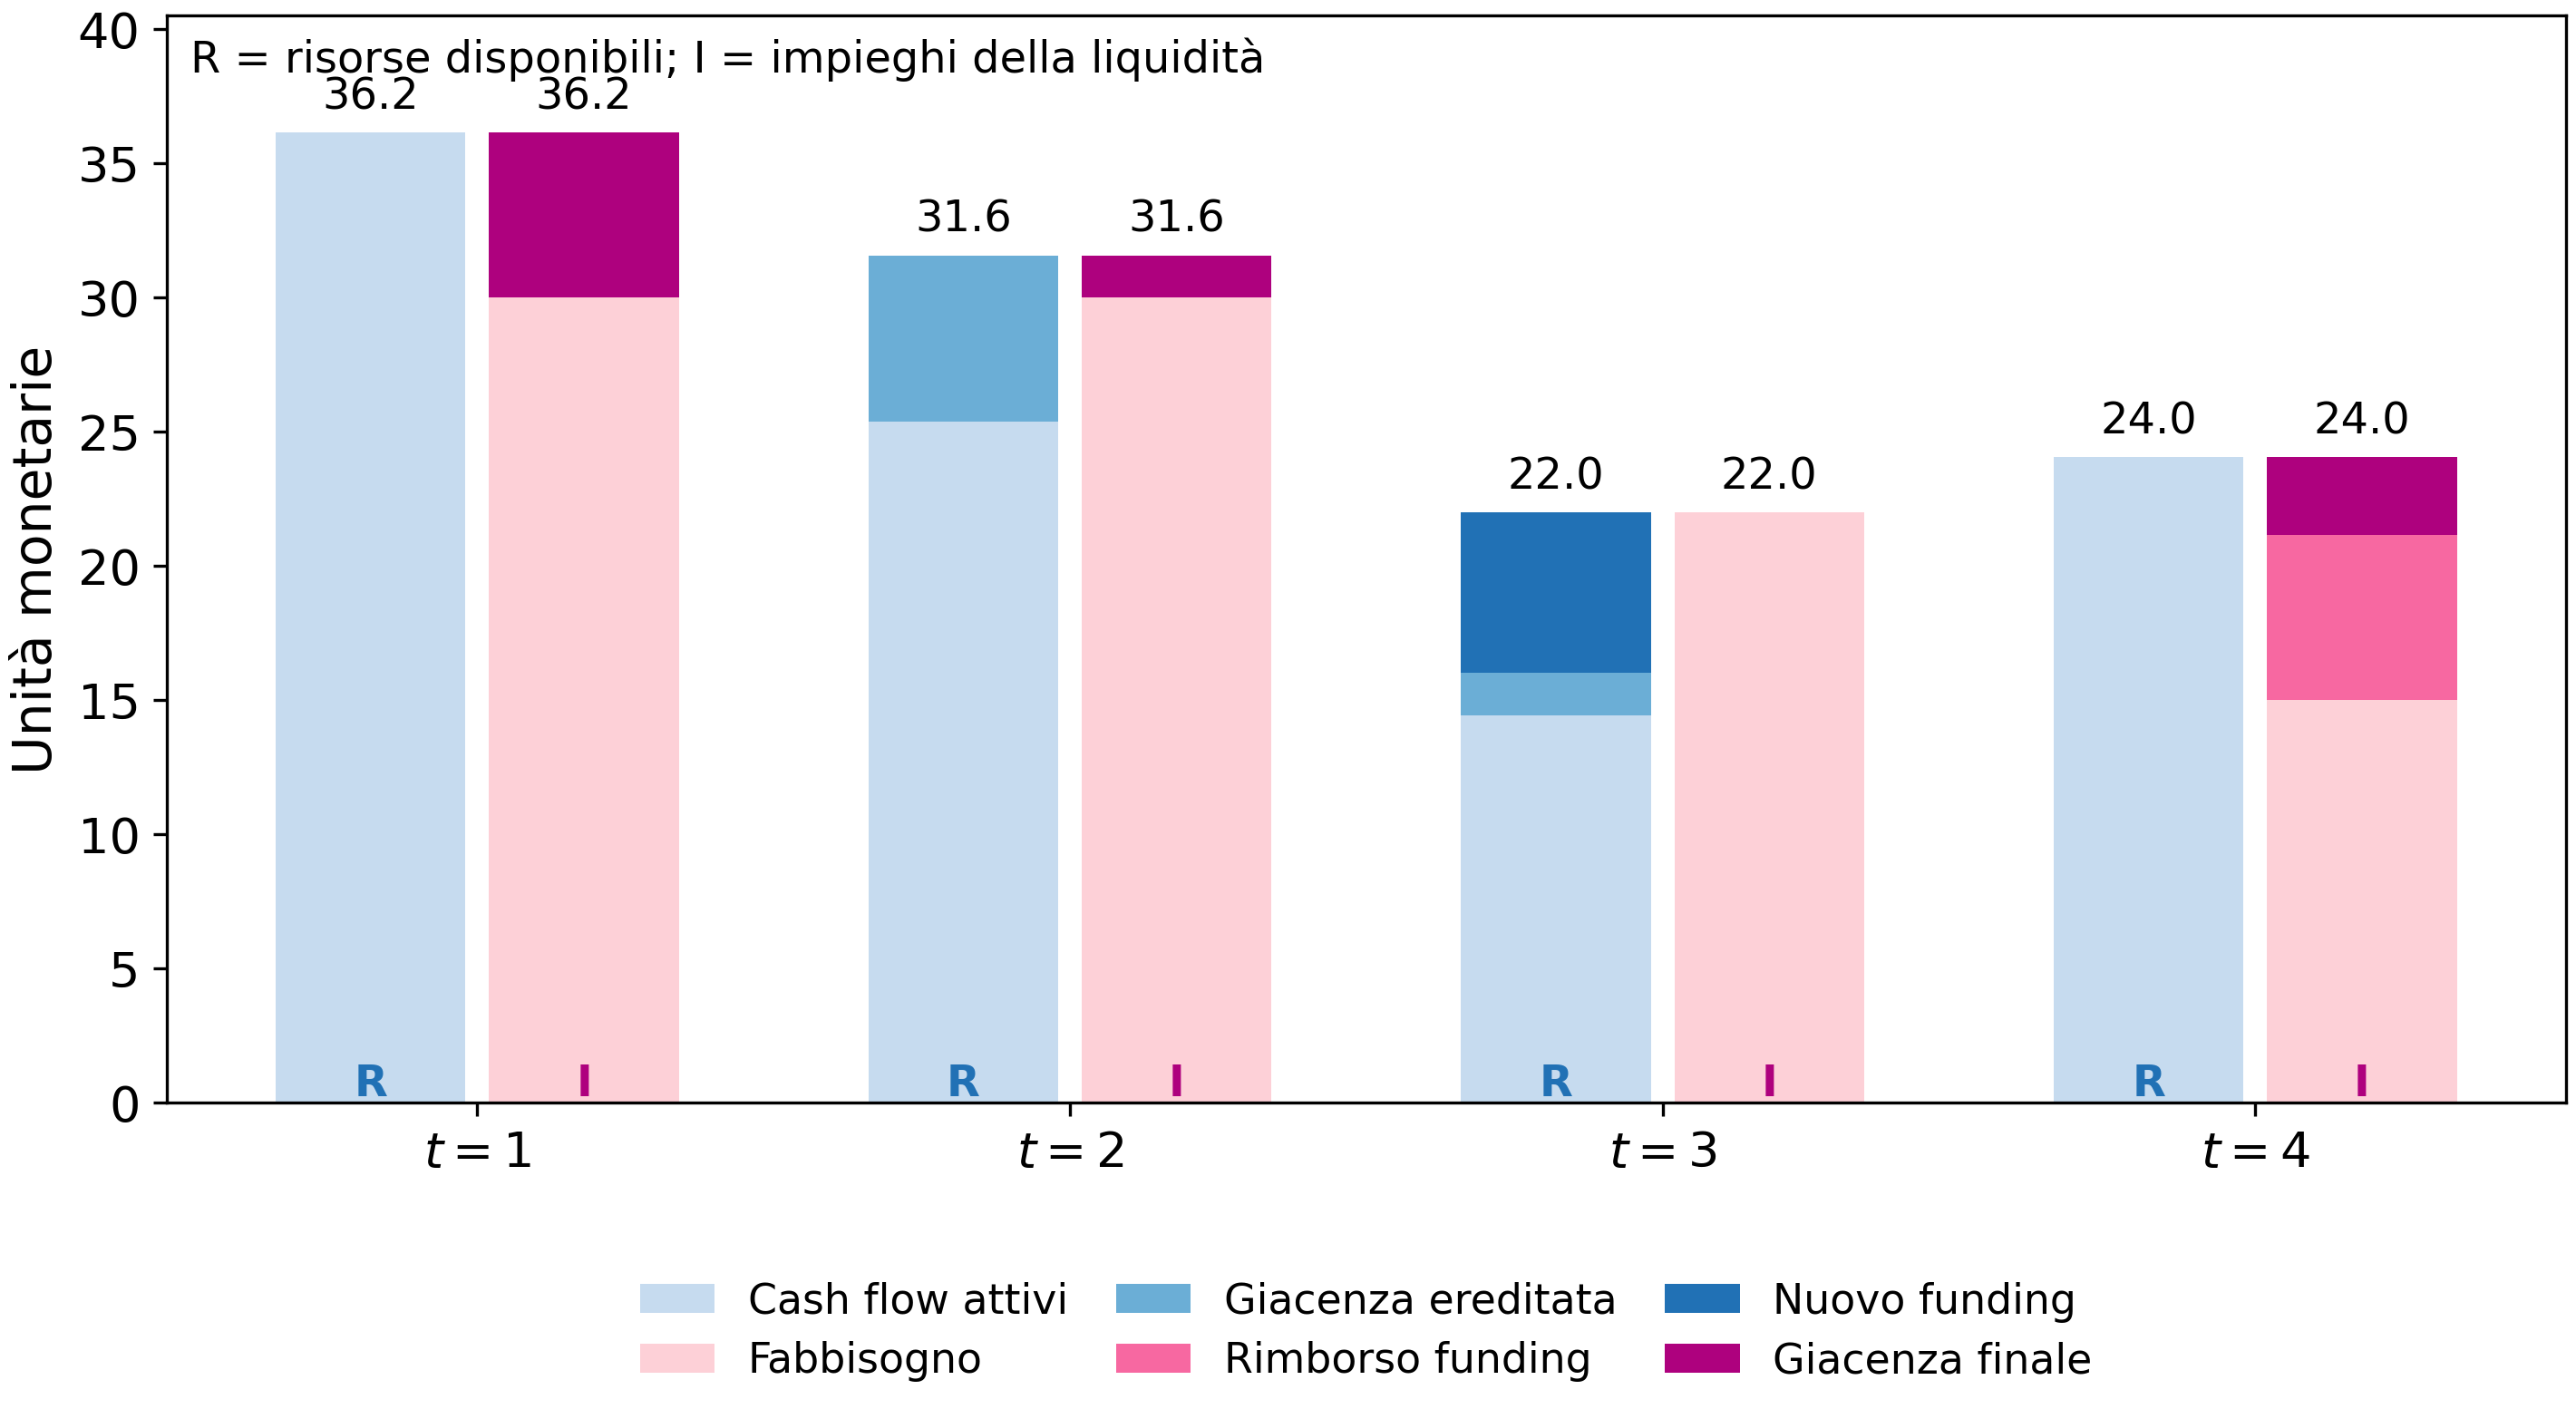
\includegraphics[width=0.94\textwidth]
{../graphics/Cap12_ALM_profili_ottimi.png}
\caption{Risorse e impieghi nelle quattro date della soluzione ottima del
caso SVB multiperiodale. La liquidit\`a accumulata trasferisce risorse verso
le date successive, mentre alla data $t=3$ il modello utilizza interamente
la capacit\`a di funding disponibile.}
\label{fig:cap12-alm-profili-ottimi}
\end{figure}

Infine, il contributo della composizione dell'attivo \`e

\[
c'x^*
\approx
3.7020,
\]

gli interessi sulle giacenze sono

\[
\sum_{t=1}^{3}r_tg_t^*
\approx
0.0402,
\]

e il costo del funding \`e

\[
\sum_{t=1}^{3}\rho_tu_t^*
=
0.1500.
\]

Pertanto,

\[
\Pi^*
\approx
3.5922.
\]

Il confronto diretto tra questo valore e il valore ottimo del problema
statico,

\[
z^{\mathrm{stat}}
\approx
3.765,
\]

non sarebbe tuttavia del tutto corretto, poich\'e la funzione obiettivo ALM
contiene anche interessi sulle giacenze e costi di funding. Per isolare
l'effetto sulla sola composizione dell'attivo \`e pi\`u informativo confrontare

\[
c'x^{\mathrm{stat}}
\approx
3.765
\]

con

\[
c'x^*
\approx
3.702.
\]

I vincoli prudenziali non risultano determinanti nella nuova soluzione:

\[
\ell'x^*
\approx
4.885
<
7,
\qquad
x_3^*=0<30.
\]

Al contrario, il limite

\[
u_3\leq6
\]

\`e raggiunto.

La sola osservazione dei vincoli attivi indica dove si concentra la scarsit\`a,
ma non ne misura ancora il valore economico. La domanda naturale diventa
quindi quale sia il valore marginale di una unit\`a aggiuntiva di risorse
disponibili nelle diverse date. Questo problema conduce direttamente
all'interpretazione duale dei bilanci temporali.

\section{Dualit\`a nell'ALM: il valore della liquidit\`a nelle diverse date}

\label{sec:cap12-dualita-alm}

Il Capitolo~\ref{cap:programmazione-lineare} ha mostrato che una variabile
duale consente di attribuire un valore marginale a una risorsa o a un
requisito del problema primale. Nel modello statico, un unico prezzo ombra
era associato al requisito aggregato di liquidit\`a.

Nel modello ALM la liquidit\`a non \`e invece concentrata in un solo vincolo.
Esiste un bilancio monetario per ciascuna data:

\[
a_t'x
+
(1+r_{t-1})g_{t-1}
+
u_t
-
(1+\rho_{t-1})u_{t-1}
-
g_t
=
d_t,
\]

con le opportune modifiche alla prima e all'ultima data.

La dualit\`a permette quindi di passare da un unico valore della liquidit\`a
a un profilo temporale di valori marginali.

\subsection{Il valore marginale dei bilanci temporali}

Associamo al bilancio della data $t$ una variabile duale

\[
\lambda_t\in\mathbb{R}.
\]

Poich\'e il vincolo di bilancio \`e un'uguaglianza, $\lambda_t$ non \`e
soggetta a un vincolo di segno.

Scrivendo il bilancio nella forma

\[
\text{risorse nette alla data }t=d_t,
\]

la convenzione adottata implica

\[
\frac{\partial\Pi^*}{\partial d_t}
=
-\lambda_t^*.
\]

Per una piccola variazione $\Delta d_t$ si ha quindi

\[
\Delta\Pi^*
\approx
-\lambda_t^*\,\Delta d_t.
\]

Se

\[
\lambda_t^*>0,
\]

un aumento unitario del fabbisogno alla data $t$ riduce localmente il
risultato ottimo di $\lambda_t^*$.

Equivalentemente, $\lambda_t^*$ misura il valore marginale di una unit\`a
aggiuntiva di liquidit\`a disponibile in quella stessa data.

Il passaggio rispetto al modello statico \`e quindi

\[
\boxed{
\text{un prezzo della liquidit\`a}
\quad\longrightarrow\quad
\text{un prezzo della liquidit\`a per ciascuna data}.
}
\]

\subsection{I valori duali nel caso SVB multiperiodale}

Per la soluzione della Sezione~\ref{sec:cap12-caso-svb-multiperiodale}, i
valori marginali dei quattro bilanci sono

\[
\lambda^*
\approx
\begin{pmatrix}
0.04524\\
0.04004\\
0.03383\\
0
\end{pmatrix}.
\]

La relazione tra posizione primale e valore marginale pu\`o essere riassunta
come segue:

\[
\begin{array}{c|c|c|c}
\hline
t & g_t^* & u_t^* & \lambda_t^*\\
\hline
1 & 6.152 & 0 & 0.04524\\
2 & 1.567 & 0 & 0.04004\\
3 & 0     & 6 & 0.03383\\
4 & 2.890 & - & 0\\
\hline
\end{array}
\]

Alla prima data, per esempio,

\[
\lambda_1^*
\approx
0.04524
\]

significa che un aumento marginale di una unit\`a del fabbisogno $d_1$
riduce il risultato ottimo di circa

\[
0.04524.
\]

Alla seconda e alla terza data il costo marginale rimane positivo, ma
diminuisce rispettivamente a

\[
0.04004
\]

e

\[
0.03383.
\]

Il risultato alla data finale richiede invece un'interpretazione specifica.

Poich\'e

\[
g_4^*
\approx
2.890>0
\]

e la giacenza terminale non riceve un valore nella funzione obiettivo, un
piccolo aumento di $d_4$ pu\`o essere assorbito semplicemente riducendo
$g_4$.

Localmente,

\[
\lambda_4^*=0.
\]

Questo non significa che la liquidit\`a alla data finale non abbia valore in
generale. Il risultato dipende dalla specificazione terminale del modello e
rimane valido finch\'e il margine rappresentato da $g_4^*$ non viene
esaurito.

\begin{figure}[htbp]
\centering
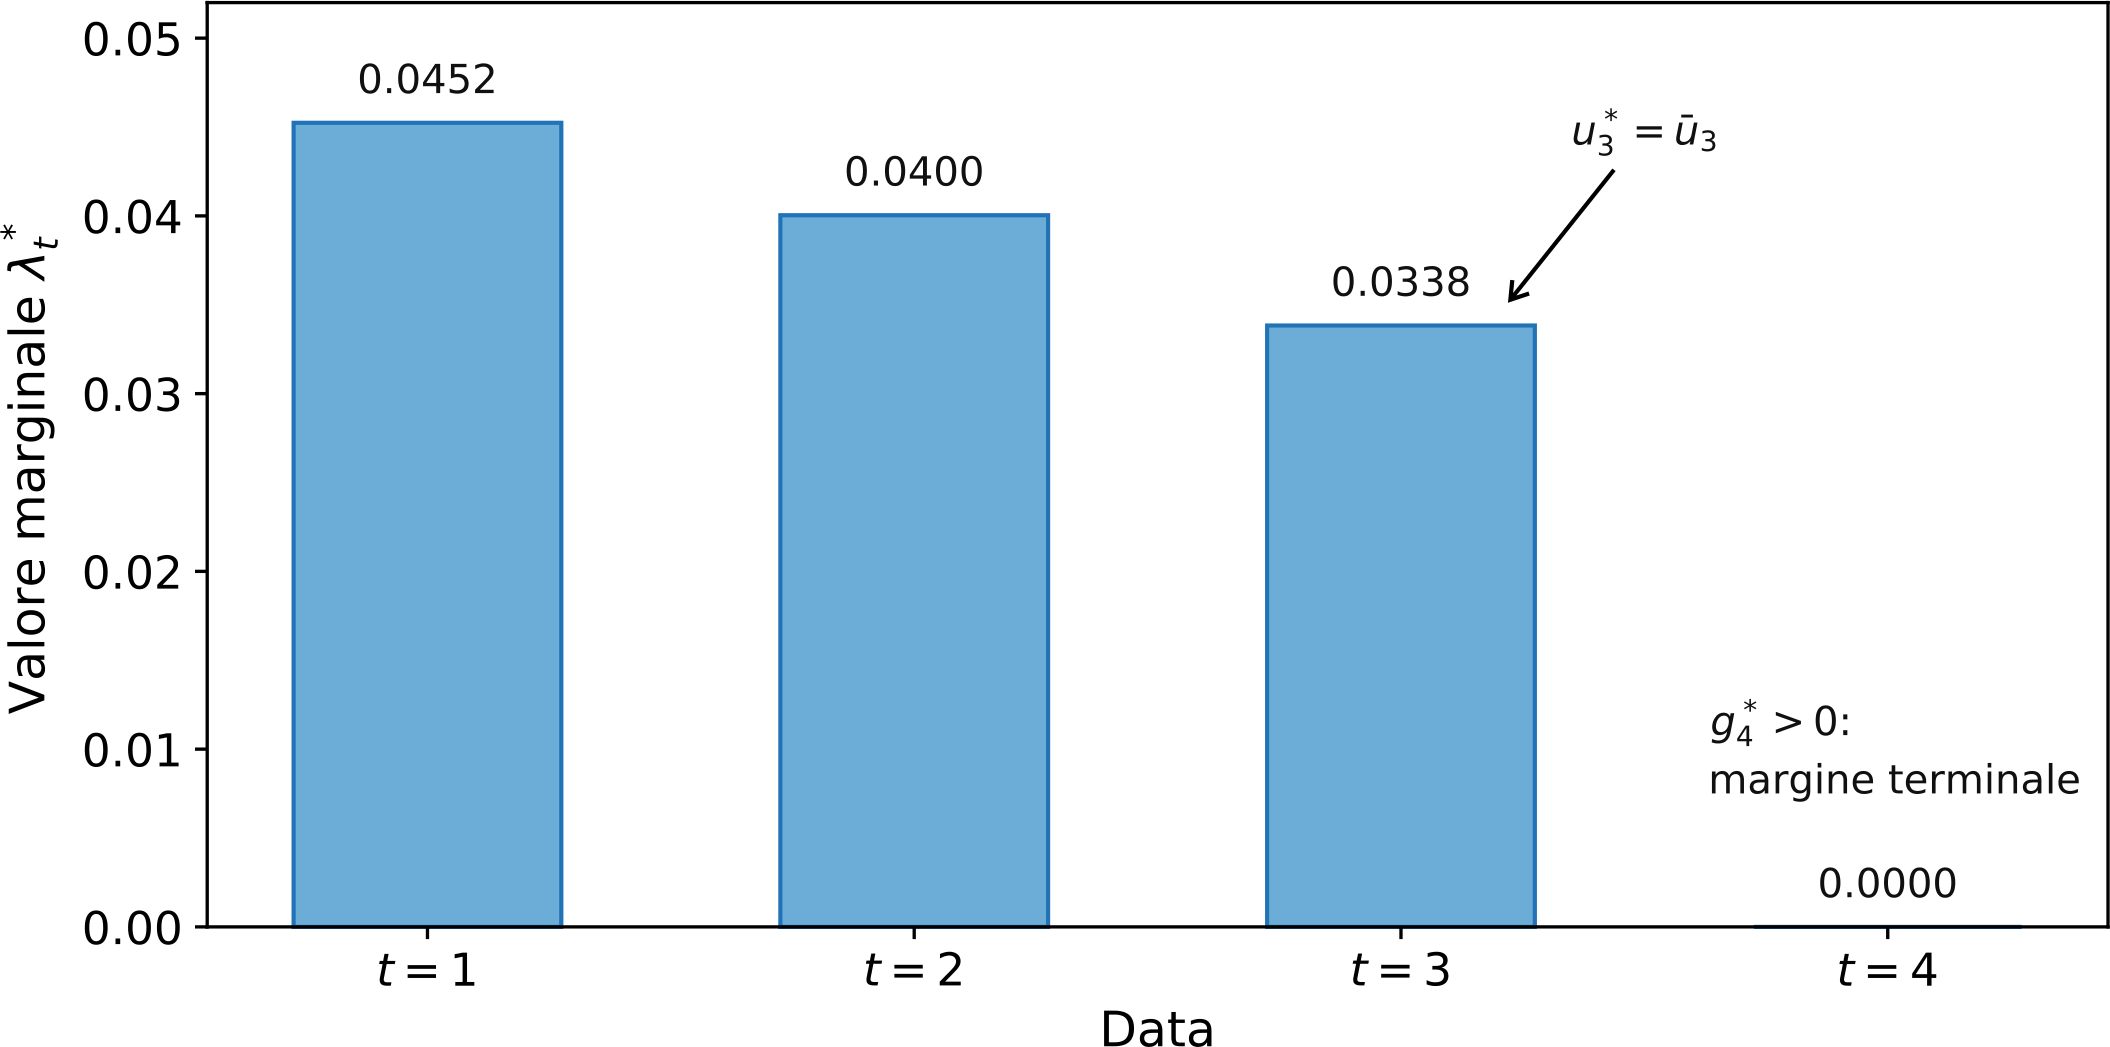
\includegraphics[width=0.88\textwidth]
{../graphics/Cap12_prezzi_ombra_scadenze.png}
\caption{Valore marginale della liquidit\`a nelle quattro date del caso SVB
multiperiodale. Il valore terminale \`e nullo localmente perch\'e la
soluzione presenta una giacenza finale positiva; alla data $t=3$ la banca
utilizza invece interamente la capacit\`a di funding disponibile.}
\label{fig:cap12-prezzi-ombra-scadenze}
\end{figure}

La Figura~\ref{fig:cap12-prezzi-ombra-scadenze} mostra un profilo decrescente
dei valori marginali. Tale andamento appartiene alla soluzione considerata e
non costituisce una propriet\`a generale dei modelli ALM: dipende dai cash
flow, dai fabbisogni, dai tassi, dai limiti di funding e dalla condizione
terminale.

\subsection{Il valore della capacit\`a di funding}

Un secondo valore duale rilevante riguarda il limite

\[
u_t\leq\bar u_t.
\]

Indichiamo con

\[
\lambda_{u,t}^*
\]

il valore marginale associato alla capacit\`a massima di funding. Localmente,

\[
\Delta\Pi^*
\approx
\lambda_{u,t}^*\,\Delta\bar u_t.
\]

Nella soluzione considerata,

\[
u_1^*<\bar u_1,
\qquad
u_2^*<\bar u_2,
\]

e i corrispondenti valori marginali sono nulli.

Alla terza data vale invece

\[
u_3^*
=
\bar u_3
=
6,
\]

e il valore duale associato al limite risulta

\[
\lambda_{u,3}^*
\approx
0.00883.
\]

Una piccola espansione della capacit\`a di funding disponibile alla data $3$
aumenterebbe quindi il valore ottimo di circa $0.00883$ per ogni unit\`a
aggiuntiva di capacit\`a.

Il risultato completa l'informazione fornita dalla soluzione primale:
l'uguaglianza

\[
u_3^*=\bar u_3
\]

individua una risorsa completamente utilizzata, mentre il corrispondente
valore duale misura quanto sarebbe economicamente utile, localmente,
allentarne il limite.

\section{Limiti del modello e passaggio all'incertezza}

\label{sec:cap12-limiti-incertezza}

Il modello sviluppato nelle sezioni precedenti permette di coordinare
composizione dell'attivo, liquidit\`a e funding lungo pi\`u date. La sua
struttura temporale \`e quindi pi\`u ricca di quella del problema statico del
Capitolo 11.

Rimane tuttavia un'ipotesi particolarmente forte: al tempo $0$ la banca
conosce l'intera traiettoria dei coefficienti che determineranno il problema
nelle date future.

\subsection{Che cosa significa deterministico}

Nel modello del capitolo sono noti al tempo $0$, tra gli altri,

\[
A^{\mathrm{CF}},
\qquad
d_t,
\qquad
r_t,
\qquad
\rho_t,
\qquad
\bar u_t.
\]

L'ipotesi deterministica non richiede che tali coefficienti siano costanti
nel tempo. Nel caso SVB multiperiodale, per esempio,

\[
r_1\neq r_2\neq r_3
\]

e anche la capacit\`a di funding varia:

\[
\bar u_1>\bar u_2>\bar u_3.
\]

Ci\`o che caratterizza il modello come deterministico \`e invece il fatto che
l'intero percorso

\[
\left\{
A^{\mathrm{CF}},
d_t,
r_t,
\rho_t,
\bar u_t
\right\}_{t=1}^{T}
\]

sia considerato noto quando il problema viene risolto.

Di conseguenza, la banca pu\`o determinare fin dal tempo $0$ l'intero piano

\[
x^*,
\qquad
g_1^*,\ldots,g_T^*,
\qquad
u_1^*,\ldots,u_{T-1}^*.
\]

Il modello risponde quindi alla domanda:

\[
\boxed{
\begin{array}{c}
\text{quale sarebbe il piano ottimo se la traiettoria futura}\\
\text{dei coefficienti fosse conosciuta?}
\end{array}
}
\]

Questa rappresentazione costituisce un benchmark utile, ma non descrive
completamente il problema decisionale affrontato da una banca reale.

\subsection{Quali elementi possono diventare incerti}

Nella realt\`a, alla data iniziale la banca non conosce con certezza le
condizioni che si manifesteranno nelle date successive.

Il vettore deterministico introdotto nella
Sezione~\ref{sec:cap12-ambiente-deterministico},

\[
\bar Z_t
=
(\bar R_t,\bar C_t,\bar F_t),
\]

pu\`o essere sostituito, in una rappresentazione incerta, da uno stato
economico-finanziario

\[
Z_t
=
(R_t,C_t,F_t).
\]

La distinzione \`e sostanziale. Nel primo caso

\[
\bar Z_t
\]

\`e un valore noto al momento della formulazione; nel secondo

\[
Z_t
\]

rappresenta uno stato futuro che non \`e ancora conosciuto al tempo $0$.

L'incertezza pu\`o quindi propagarsi ai coefficienti dell'ALM. In forma
schematica,

\[
Z_t
\quad\longrightarrow\quad
r_t,\ \rho_t,\ \bar u_t,
\]

e, quando economicamente appropriato, anche ai cash flow disponibili e ai
fabbisogni.

In particolare, il fabbisogno deterministico

\[
d_t
\]

pu\`o essere sostituito da una quantit\`a futura

\[
D_t,
\]

il cui valore dipende dalle condizioni che si realizzano.

La struttura concettuale discussa nella
Sezione~\ref{sec:cap12-stato-banca} suggerisce pi\`u precisamente

\[
D_t
=
d(Z_t,h_t),
\]

dove

\[
h_t
=
h(X_t,Z_t)
\]

dipende sia dall'ambiente esterno sia dallo stato della banca.

Non renderemo qui operative queste relazioni. Esse servono a individuare il
punto nel quale l'ipotesi deterministica dovr\`a essere abbandonata.

\subsection{Dal piano unico alle decisioni contingenti}

L'effetto pi\`u importante dell'incertezza riguarda la natura stessa delle
decisioni.

Nel modello deterministico il valore futuro di

\[
u_t
\]

pu\`o essere scelto gi\`a al tempo $0$, perch\'e i fabbisogni, i costi e la
capacit\`a di funding futuri sono noti.

In presenza di incertezza questa impostazione non \`e generalmente
appropriata. Il funding da utilizzare alla data $t$ dovrebbe poter dipendere
dalle condizioni effettivamente osservate a quella data.

Si passa quindi concettualmente da

\[
u_t
=
\text{numero fissato al tempo }0
\]

a una decisione del tipo

\[
u_t
=
u_t(\text{informazione disponibile alla data }t).
\]

La composizione iniziale $x$, invece, deve essere scelta prima di conoscere
gli stati futuri. Essa deve quindi tenere conto delle conseguenze che potranno
emergere lungo pi\`u evoluzioni possibili.

Il passaggio fondamentale pu\`o essere sintetizzato come

\[
\boxed{
\begin{array}{ccc}
\text{ALM deterministico}
&
\longrightarrow
&
\text{ALM sotto incertezza}
\\[4pt]
\text{una traiettoria nota}
&&
\text{pi\`u evoluzioni possibili}
\\[4pt]
\text{un piano fissato al tempo }0
&&
\text{decisioni compatibili con l'informazione disponibile}.
\end{array}
}
\]

Anche i valori duali ottenuti nelle sezioni precedenti devono essere letti
alla luce di questa distinzione. Essi misurano valori marginali
\emph{condizionati alla traiettoria deterministica assunta}: non incorporano
da soli il rischio che tassi, fabbisogni o disponibilit\`a di funding seguano
percorsi differenti.

Il modello deterministico rimane quindi un riferimento essenziale. Permette
di isolare la struttura dei bilanci intertemporali, identificare le date nelle
quali le risorse risultano scarse e attribuire loro un valore marginale.

Il passo successivo consiste nel mantenere questa struttura temporale
abbandonando l'ipotesi di conoscenza perfetta del futuro.

\section{Esercizi svolti}

\label{sec:cap12-esercizi-svolti}

Gli esercizi seguenti consolidano tre passaggi centrali del capitolo:
la formulazione di un problema ALM, la verifica della fattibilit\`a
intertemporale e l'interpretazione dei valori duali.

\begin{exercise}[Dalla descrizione del problema alla formulazione]

\label{ex:cap12-formulazione-alm-solver}

Una banca dispone al tempo $0$ di $50$ unit\`a monetarie, che devono essere
interamente allocate tra tre classi di attivo.

La prima classe rappresenta cassa e riserve. Produce un contributo economico
pari all'1\% dell'investimento e l'intero ammontare investito diventa
disponibile come liquidit\`a alla data $1$.

La seconda classe \`e costituita da titoli a breve scadenza. Produce un
contributo economico del $2.5\%$; il $60\%$ dell'investimento iniziale diventa
disponibile alla data $1$ e il restante $40\%$ alla data $2$.

La terza classe \`e costituita da prestiti. Produce un contributo economico
del $4.5\%$; il $10\%$ dell'investimento iniziale diventa disponibile alla
data $1$, il $30\%$ alla data $2$ e il restante $60\%$ alla data $3$.

I fabbisogni di liquidit\`a alle tre date sono rispettivamente

\[
25,\qquad18,\qquad12.
\]

La liquidit\`a non utilizzata alla data $1$ pu\`o essere trasferita alla data
$2$ con un rendimento dello $0.5\%$; quella non utilizzata alla data $2$ pu\`o
essere trasferita alla data $3$ con un rendimento dello $0.6\%$.

La banca pu\`o inoltre raccogliere funding alla data $1$ fino a un massimo di
$4$ unit\`a, con costo dell'1.5\%, e alla data $2$ fino a un massimo di $3$
unit\`a, con costo del $2\%$. Il funding raccolto in una data deve essere
rimborsato alla data successiva.

In uno scenario di stress, le perdite unitarie associate alle tre classi di
attivo sono rispettivamente

\[
0,\qquad0.03,\qquad0.08,
\]

e la perdita complessiva non pu\`o superare $2.6$.

Infine, l'investimento nei prestiti non pu\`o superare $25$ unit\`a.

A partire esclusivamente da queste informazioni:

\begin{enumerate}

\item individuare le variabili decisionali;

\item costruire i vettori e la matrice dei parametri necessari;

\item formulare matematicamente la funzione obiettivo;

\item scrivere il vincolo sulle risorse iniziali, i tre bilanci di liquidit\`a,
i vincoli prudenziali, i limiti sul funding e le condizioni di non negativit\`a;

\item raccogliere tutte le variabili in un unico vettore $z$ e scrivere il
problema nella forma matriciale necessaria per l'utilizzo di un solver LP:

\[
\min\;\widetilde c'z,
\qquad
A_{\mathrm{ub}}z\leq b_{\mathrm{ub}},
\qquad
A_{\mathrm{eq}}z=b_{\mathrm{eq}},
\]

specificando inoltre i bounds delle variabili.
\end{enumerate}

\end{exercise}

\noindent
\textbf{Soluzione.}

\begin{enumerate}

\item \textbf{Variabili decisionali.}

Indichiamo con

\[
x_1,\qquad x_2,\qquad x_3
\]

gli importi investiti al tempo $0$ rispettivamente in cassa e riserve,
titoli a breve scadenza e prestiti.

Le giacenze di liquidit\`a residue alle tre date sono

\[
g_1,\qquad g_2,\qquad g_3,
\]

mentre il funding raccolto alle prime due date \`e rappresentato da

\[
u_1,\qquad u_2.
\]

Non viene introdotto nuovo funding alla data finale, poich\'e il relativo
rimborso cadrebbe oltre l'orizzonte del modello.

Tutte le variabili sono non negative:

\[
x_j\geq0,
\qquad
j=1,2,3,
\]

\[
g_t\geq0,
\qquad
t=1,2,3,
\]

\[
u_t\geq0,
\qquad
t=1,2.
\]


\item \textbf{Costruzione dei parametri.}

Dalla descrizione delle tre classi di attivo si ricava il vettore dei
contributi economici unitari

\[
c
=
\begin{pmatrix}
0.010\\
0.025\\
0.045
\end{pmatrix}.
\]

I profili temporali con cui le risorse investite nelle tre classi diventano
disponibili determinano la matrice dei cash flow

\[
A^{\mathrm{CF}}
=
\begin{pmatrix}
1.00 & 0.60 & 0.10\\
0    & 0.40 & 0.30\\
0    & 0    & 0.60
\end{pmatrix}.
\]

Il vettore dei fabbisogni \`e

\[
d
=
\begin{pmatrix}
25\\
18\\
12
\end{pmatrix}.
\]

I rendimenti delle giacenze sono

\[
r_1=0.005,
\qquad
r_2=0.006,
\]

mentre i costi del funding sono

\[
\rho_1=0.015,
\qquad
\rho_2=0.020.
\]

La capacit\`a massima di funding \`e

\[
\bar u_1=4,
\qquad
\bar u_2=3.
\]

Il vettore delle perdite unitarie nello scenario di stress \`e

\[
\ell
=
\begin{pmatrix}
0\\
0.03\\
0.08
\end{pmatrix},
\]

con limite complessivo

\[
K=2.6.
\]

Infine, il limite di concentrazione sui prestiti \`e

\[
x_3\leq25.
\]


\item \textbf{Funzione obiettivo.}

In forma simbolica, per un orizzonte con $T=3$ date future, la funzione
obiettivo \`e

\[
\max\;
\Pi(x,g,u)
=
c'x
+
\sum_{t=1}^{2}r_tg_t
-
\sum_{t=1}^{2}\rho_tu_t.
\]

Sostituendo i valori numerici si ottiene

\[
\boxed{
\max\;
0.010x_1
+
0.025x_2
+
0.045x_3
+
0.005g_1
+
0.006g_2
-
0.015u_1
-
0.020u_2.
}
\]


\item \textbf{Vincoli del modello ALM.}

Le risorse iniziali devono essere interamente allocate:

\[
x_1+x_2+x_3=50.
\]

Alla prima data sono disponibili i cash flow prodotti dagli attivi e il
funding eventualmente raccolto in $t=1$. Il bilancio di liquidit\`a \`e

\[
x_1
+
0.60x_2
+
0.10x_3
+
u_1
=
25+g_1,
\]

ovvero

\[
x_1
+
0.60x_2
+
0.10x_3
+
u_1
-
g_1
=
25.
\]

Alla seconda data diventano disponibili i nuovi cash flow degli attivi, la
giacenza precedente capitalizzata e il nuovo funding. Deve inoltre essere
rimborsato il funding raccolto alla prima data:

\[
0.40x_2
+
0.30x_3
+
1.005g_1
+
u_2
=
18
+
1.015u_1
+
g_2.
\]

Pertanto,

\[
0.40x_2
+
0.30x_3
+
1.005g_1
+
u_2
-
1.015u_1
-
g_2
=
18.
\]

Alla data finale non viene raccolto nuovo funding:

\[
0.60x_3
+
1.006g_2
=
12
+
1.020u_2
+
g_3,
\]

ossia

\[
0.60x_3
+
1.006g_2
-
1.020u_2
-
g_3
=
12.
\]

Il vincolo sulla perdita nello scenario di stress \`e

\[
0.03x_2+0.08x_3\leq2.6.
\]

Il limite di concentrazione sui prestiti \`e

\[
x_3\leq25.
\]

I limiti sul funding sono

\[
0\leq u_1\leq4,
\qquad
0\leq u_2\leq3.
\]

Infine,

\[
x_1,x_2,x_3\geq0,
\qquad
g_1,g_2,g_3\geq0.
\]

Il programma lineare completo \`e quindi

\[
\begin{array}{ll}

\max
&
\displaystyle
0.010x_1
+
0.025x_2
+
0.045x_3
\\
& +
0.005g_1
+
0.006g_2
-
0.015u_1
-
0.020u_2
\\[8pt]

\mbox{soggetto a}
&
x_1+x_2+x_3=50,
\\[6pt]

&
x_1+0.60x_2+0.10x_3+u_1-g_1=25,
\\[6pt]

&
0.40x_2+0.30x_3+1.005g_1
+u_2-1.015u_1-g_2=18,
\\[6pt]

&
0.60x_3+1.006g_2-1.020u_2-g_3=12,
\\[6pt]

&
0.03x_2+0.08x_3\leq2.6,
\\[6pt]

&
x_3\leq25,
\\[6pt]

&
0\leq u_1\leq4,
\qquad
0\leq u_2\leq3,
\\[6pt]

&
x_1,x_2,x_3,g_1,g_2,g_3\geq0.
\end{array}
\]


\item \textbf{Forma matriciale per il solver.}

Raccogliamo le variabili secondo l'ordine

\[
z
=
\begin{pmatrix}
x_1&
x_2&
x_3&
g_1&
g_2&
g_3&
u_1&
u_2
\end{pmatrix}'.
\]

Rispetto a questo ordinamento, il vettore dei coefficienti della funzione
obiettivo in massimizzazione \`e

\[
c^{\mathrm{ALM}}
=
\begin{pmatrix}
0.010\\
0.025\\
0.045\\
0.005\\
0.006\\
0\\
-0.015\\
-0.020
\end{pmatrix}.
\]

Poich\'e il solver \texttt{scipy.optimize.linprog} utilizza una formulazione
in minimizzazione, si pone

\[
\widetilde c
=
-c^{\mathrm{ALM}},
\]

e quindi

\[
\widetilde c
=
\begin{pmatrix}
-0.010\\
-0.025\\
-0.045\\
-0.005\\
-0.006\\
0\\
0.015\\
0.020
\end{pmatrix}.
\]

Il problema passato al solver ha pertanto funzione obiettivo

\[
\min\;\widetilde c'z.
\]

Il vincolo sulle risorse iniziali e i tre bilanci temporali sono uguaglianze.
Essi possono essere raccolti nella matrice

\[
A_{\mathrm{eq}}
=
\begin{pmatrix}
1 & 1    & 1    & 0     & 0     & 0  & 0      & 0\\
1 & 0.60 & 0.10 & -1    & 0     & 0  & 1      & 0\\
0 & 0.40 & 0.30 & 1.005 & -1    & 0  & -1.015 & 1\\
0 & 0    & 0.60 & 0     & 1.006 & -1 & 0      & -1.020
\end{pmatrix},
\]

con

\[
b_{\mathrm{eq}}
=
\begin{pmatrix}
50\\
25\\
18\\
12
\end{pmatrix}.
\]

I due vincoli espressi come disuguaglianze sono

\[
0.03x_2+0.08x_3\leq2.6
\]

e

\[
x_3\leq25.
\]

Pertanto,

\[
A_{\mathrm{ub}}
=
\begin{pmatrix}
0 & 0.03 & 0.08 & 0 & 0 & 0 & 0 & 0\\
0 & 0    & 1    & 0 & 0 & 0 & 0 & 0
\end{pmatrix},
\]

e

\[
b_{\mathrm{ub}}
=
\begin{pmatrix}
2.6\\
25
\end{pmatrix}.
\]

Infine, i limiti delle variabili sono

\[
\begin{array}{c|c}
\text{variabili} & \text{bounds}\\
\hline
x_1,x_2,x_3 & [0,+\infty)\\
g_1,g_2,g_3 & [0,+\infty)\\
u_1 & [0,4]\\
u_2 & [0,3].
\end{array}
\]

La formulazione da trasmettere al solver \`e quindi completamente
specificata da

\[
\boxed{
\begin{array}{c}
\displaystyle
\min\;\widetilde c'z
\\[6pt]
A_{\mathrm{eq}}z=b_{\mathrm{eq}},
\\[4pt]
A_{\mathrm{ub}}z\leq b_{\mathrm{ub}},
\\[4pt]
\underline z\leq z\leq\overline z.
\end{array}
}
\]

Il passaggio decisivo non consiste nell'applicazione del solver, ma nella
traduzione coerente della descrizione finanziaria in variabili, coefficienti
e vincoli. Una volta costruita correttamente questa rappresentazione, il
problema \`e un programma lineare standard e pu\`o essere risolto
numericamente senza ulteriori modifiche alla sua struttura economica.

\end{enumerate}


\begin{exercise}[Fattibilit\`a temporale e limite al funding]

\label{ex:cap12-fattibilita-funding}

Una banca ha investito al tempo $0$ in due classi di attivo secondo la
composizione

\[
x=
\begin{pmatrix}
20\\
20
\end{pmatrix}.
\]

La distribuzione temporale dei cash flow prodotti dagli attivi \`e descritta
dalla matrice

\[
A^{\mathrm{CF}}
=
\begin{pmatrix}
0.70 & 0.10\\
0.30 & 0.30\\
0    & 0.60
\end{pmatrix}.
\]

I fabbisogni di liquidit\`a alle tre date sono

\[
d'
=
(15,\;14,\;8).
\]

La liquidit\`a residua alla prima data pu\`o essere trasferita alla seconda
con rendimento

\[
r_1=0.005.
\]

Si assume che non venga raccolto funding alla prima data,

\[
u_1=0,
\]

mentre alla seconda data la banca pu\`o ricorrere a funding che dovr\`a essere
rimborsato alla data finale con costo

\[
\rho_2=0.020.
\]

In condizioni ordinarie la capacit\`a di funding alla seconda data \`e

\[
\bar u_2=3.
\]

\begin{enumerate}

\item Calcolare il profilo temporale dei cash flow prodotto dagli attivi.

\item Verificare se la composizione assegnata permette di soddisfare i
fabbisogni alle tre date senza ricorrere al funding.

\item Determinare il funding minimo necessario alla seconda data e calcolare
la giacenza terminale risultante.

\item Supporre ora che la capacit\`a massima di funding alla seconda data si
riduca a

\[
\bar u_2=0.8.
\]

Stabilire se il piano rimane ammissibile e interpretare il risultato.

\end{enumerate}

\end{exercise}

\noindent
\textbf{Soluzione.}

\begin{enumerate}

\item Il profilo dei cash flow \`e

\[
A^{\mathrm{CF}}x
=
\begin{pmatrix}
0.70 & 0.10\\
0.30 & 0.30\\
0    & 0.60
\end{pmatrix}
\begin{pmatrix}
20\\
20
\end{pmatrix}
=
\begin{pmatrix}
16\\
12\\
12
\end{pmatrix}.
\]

\item Alla prima data, ponendo $u_1=0$,

\[
16=15+g_1,
\]

da cui

\[
g_1=1.
\]

Alla seconda data, in assenza di funding, le risorse disponibili sarebbero

\[
12+1.005(1)
=
13.005.
\]

Il fabbisogno \`e invece

\[
d_2=14.
\]

Pertanto

\[
13.005<14
\]

e la composizione non \`e temporalmente fattibile senza funding.

Il punto importante \`e che l'insufficienza emerge alla seconda data:
non pu\`o essere compensata utilizzando anticipatamente il cash flow pari a
$12$ che sar\`a disponibile soltanto alla data successiva.

\item Ponendo $g_2=0$, il bilancio della seconda data richiede

\[
12
+
1.005(1)
+
u_2
=
14.
\]

Il funding minimo \`e quindi

\[
u_2
=
14-13.005
=
0.995.
\]

Alla data finale il rimborso dovuto \`e

\[
1.020(0.995)
=
1.0149.
\]

Il bilancio terminale diventa

\[
12
=
8
+
1.0149
+
g_3,
\]

da cui

\[
g_3
=
2.9851.
\]

Il funding anticipa quindi $0.995$ unit\`a alla seconda data e genera alla
terza un rimborso pari a $1.0149$.

\item Se

\[
\bar u_2=0.8,
\]

il funding massimo disponibile sarebbe inferiore al fabbisogno minimo

\[
u_2^{\min}=0.995.
\]

La composizione considerata diventerebbe quindi non ammissibile:

\[
\bar u_2<u_2^{\min}.
\]

\end{enumerate}

L'esercizio distingue due concetti che non devono essere confusi:
l'esistenza di risorse lungo l'intero orizzonte e la loro disponibilit\`a
nella data nella quale devono essere utilizzate.


\begin{exercise}[Interpretazione dei valori duali]

\label{ex:cap12-valori-duali}

Nel caso SVB multiperiodale della
Sezione~\ref{sec:cap12-caso-svb-multiperiodale}, i valori marginali associati
ai quattro bilanci temporali sono

\[
\lambda^*
\approx
\begin{pmatrix}
0.04524\\
0.04004\\
0.03383\\
0
\end{pmatrix}.
\]

Il valore duale associato al limite

\[
u_3\leq\bar u_3
\]

\`e inoltre

\[
\lambda_{u,3}^*
\approx
0.00883.
\]

Si assuma che le variazioni considerate siano sufficientemente piccole da
non modificare la struttura della soluzione ottima.

\begin{enumerate}

\item Stimare l'effetto sul valore ottimo di un aumento

\[
\Delta d_2=0.5.
\]

\item Interpretare il risultato

\[
\lambda_4^*=0
\]

sapendo che

\[
g_4^*\approx2.890.
\]

\item Stimare l'effetto di un aumento unitario della capacit\`a di funding
alla terza data.

\item Spiegare perch\'e queste valutazioni devono essere interpretate
localmente.

\end{enumerate}

\end{exercise}

\noindent
\textbf{Soluzione.}

\begin{enumerate}

\item Per una piccola variazione del fabbisogno vale

\[
\Delta\Pi^*
\approx
-\lambda_2^*\,\Delta d_2.
\]

Pertanto

\[
\Delta\Pi^*
\approx
-0.04004(0.5)
=
-0.02002.
\]

Un aumento di mezzo punto del fabbisogno alla seconda data riduce quindi
localmente il valore ottimo di circa $0.020$.

\item Il risultato

\[
\lambda_4^*=0
\]

non significa che la liquidit\`a alla data finale sia priva di significato
finanziario.

Nella soluzione considerata esiste infatti una giacenza terminale positiva:

\[
g_4^*\approx2.890.
\]

Un piccolo aumento di $d_4$ pu\`o essere assorbito riducendo questa giacenza,
senza richiedere una modifica della composizione dell'attivo o del piano di
funding e senza modificare localmente la funzione obiettivo.

Il valore marginale nullo riflette quindi l'esistenza di un margine terminale
nella soluzione considerata.

\item Per il limite sulla capacit\`a di funding vale localmente

\[
\Delta\Pi^*
\approx
\lambda_{u,3}^*
\Delta\bar u_3.
\]

Con

\[
\Delta\bar u_3=1
\]

si ottiene

\[
\Delta\Pi^*
\approx
0.00883.
\]

Una unit\`a aggiuntiva di capacit\`a di funding alla terza data aumenterebbe
quindi il risultato massimo di circa $0.00883$.

\item I valori duali descrivono la pendenza locale della funzione valore
rispetto ai termini noti o ai limiti considerati.

Se una variazione sufficientemente ampia modifica i vincoli determinanti
della soluzione, anche i corrispondenti valori marginali possono cambiare.
Non \`e quindi corretto utilizzare indefinitamente lo stesso prezzo ombra
per variazioni arbitrarie dei parametri.

\end{enumerate}

Il confronto tra soluzione primale e valori duali mette in evidenza due
informazioni complementari: il primale mostra come vengono impiegate le
risorse disponibili, mentre il duale quantifica il valore marginale di una
variazione dei requisiti o delle risorse scarse.

\section{Esercizi proposti}

\label{sec:cap12-esercizi-proposti}


\begin{exercise}[Cash flow aggregati e distribuzione temporale]

\label{ex:cap12-proposto-cashflow-temporali}

Una banca considera tre classi di attivo. La matrice dei cash flow \`e

\[
A^{\mathrm{CF}}
=
\begin{pmatrix}
0.80 & 0.30 & 0.10\\
0.20 & 0.40 & 0.30\\
0    & 0.30 & 0.60
\end{pmatrix},
\]

e la composizione iniziale \`e

\[
x'
=
(10,\;20,\;30).
\]

I fabbisogni sono

\[
d'
=
(16,\;21,\;18).
\]

Si assumano, per semplicit\`a,

\[
r_1=r_2=0.
\]

Alla seconda data la banca pu\`o raccogliere funding al tasso

\[
\rho_2=0.02.
\]

\begin{enumerate}

\item Calcolare il profilo temporale

\[
A^{\mathrm{CF}}x.
\]

\item Verificare che il cash flow complessivo prodotto lungo l'orizzonte
coincida con l'ammontare inizialmente investito.

\item Stabilire se i fabbisogni possono essere soddisfatti senza funding,
tenendo conto del trasferimento delle giacenze tra date consecutive.

\item Determinare il funding minimo necessario alla seconda data e la
giacenza terminale risultante.

\item Spiegare perch\'e il confronto tra

\[
\sum_t d_t
\]

e il cash flow complessivo dell'attivo non \`e sufficiente per stabilire
l'ammissibilit\`a del piano.

\end{enumerate}

\end{exercise}

\noindent
\textit{Risultati:}

\[
A^{\mathrm{CF}}x
=
\begin{pmatrix}
17\\
19\\
24
\end{pmatrix},
\qquad
\sum_{t=1}^{3}(A^{\mathrm{CF}}x)_t=60.
\]

Alla prima data

\[
g_1=1.
\]

Alla seconda data rimane un deficit pari a $1$, per cui il funding minimo
\`e

\[
u_2=1.
\]

Tenendo conto del rimborso alla data finale,

\[
g_3=24-18-1.02=4.98.
\]


\begin{exercise}[Due portafogli con diversa struttura temporale]

\label{ex:cap12-proposto-confronto-portafogli}

Si consideri la matrice

\[
A^{\mathrm{CF}}
=
\begin{pmatrix}
0.90 & 0.40 & 0.10\\
0.10 & 0.40 & 0.30\\
0    & 0.20 & 0.60
\end{pmatrix}
\]

e i due portafogli

\[
x^{(A)}
=
\begin{pmatrix}
20\\
20\\
10
\end{pmatrix},
\qquad
x^{(B)}
=
\begin{pmatrix}
10\\
20\\
20
\end{pmatrix}.
\]

Entrambi utilizzano risorse iniziali pari a

\[
A_0=50.
\]

I fabbisogni sono

\[
d'
=
(22,\;16,\;10).
\]

I parametri finanziari sono

\[
r_1=0.004,
\qquad
r_2=0.005,
\]

\[
\rho_1=0.014,
\qquad
\rho_2=0.018,
\]

con

\[
\bar u_1=5,
\qquad
\bar u_2=4.
\]

\begin{enumerate}

\item Calcolare i profili

\[
A^{\mathrm{CF}}x^{(A)}
\qquad\text{e}\qquad
A^{\mathrm{CF}}x^{(B)}.
\]

\item Verificare se il portafoglio $A$ pu\`o soddisfare i tre fabbisogni
senza ricorrere al funding.

\item Per il portafoglio $B$, determinare il funding minimo necessario alla
prima data.

\item Verificare se la capacit\`a massima di funding alla seconda data
permette di proseguire il piano.

\item Interpretare la differenza tra i due portafogli dal punto di vista
dell'ALM.

\end{enumerate}

\end{exercise}

\noindent
\textit{Risultati:}

\[
A^{\mathrm{CF}}x^{(A)}
=
\begin{pmatrix}
27\\
13\\
10
\end{pmatrix},
\qquad
A^{\mathrm{CF}}x^{(B)}
=
\begin{pmatrix}
19\\
15\\
16
\end{pmatrix}.
\]

Il portafoglio $A$ \`e finanziariamente ammissibile senza funding.

Per il portafoglio $B$ occorre alla prima data

\[
u_1=3.
\]

Alla seconda data il funding minimo richiesto \`e circa

\[
u_2=4.042,
\]

ma

\[
\bar u_2=4.
\]

Il portafoglio $B$ non \`e quindi ammissibile.


\begin{exercise}[Formulazione completa di un problema ALM]

\label{ex:cap12-proposto-formulazione-completa}

Una banca dispone di

\[
A_0=50
\]

unit\`a monetarie e pu\`o scegliere tra tre classi di attivo.

I parametri dell'attivo sono

\[
\begin{array}{c|cc}
\hline
j & c_j & \ell_j\\
\hline
1 & 0.015 & 0\\
2 & 0.030 & 0.04\\
3 & 0.045 & 0.10\\
\hline
\end{array}
\]

e

\[
A^{\mathrm{CF}}
=
\begin{pmatrix}
0.90 & 0.40 & 0.10\\
0.10 & 0.40 & 0.30\\
0    & 0.20 & 0.60
\end{pmatrix}.
\]

I parametri temporali sono

\[
\begin{array}{c|cccc}
\hline
t & d_t & r_t & \rho_t & \bar u_t\\
\hline
1 & 20 & 0.004 & 0.014 & 5\\
2 & 18 & 0.005 & 0.018 & 4\\
3 & 10 & -     & -     & -\\
\hline
\end{array}
\]

e il limite alla perdita sotto stress \`e

\[
\ell'x\leq3.2.
\]

La terza classe di attivo non pu\`o inoltre superare

\[
x_3\leq20.
\]

\begin{enumerate}

\item Individuare tutte le variabili decisionali.

\item Scrivere la funzione obiettivo prima in forma simbolica e poi in forma
numerica.

\item Scrivere il vincolo sulle risorse iniziali.

\item Scrivere i tre bilanci di liquidit\`a prima in forma simbolica e poi
sostituendo i coefficienti numerici.

\item Completare il programma lineare con i limiti di funding, il vincolo di
stress, il limite di concentrazione e le condizioni di non negativit\`a.

\item Indicare quali coefficienti del modello potrebbero dipendere
dall'ambiente economico-finanziario

\[
\bar Z_t=(\bar R_t,\bar C_t,\bar F_t).
\]

\end{enumerate}

\end{exercise}

\noindent
\textit{Risultati di controllo:} le variabili sono

\[
x_1,x_2,x_3,
\qquad
g_1,g_2,g_3,
\qquad
u_1,u_2.
\]

La funzione obiettivo numerica \`e

\[
\max\;
0.015x_1+0.030x_2+0.045x_3
+0.004g_1+0.005g_2
-0.014u_1-0.018u_2.
\]

Il primo bilancio \`e

\[
0.90x_1+0.40x_2+0.10x_3+u_1-g_1=20.
\]


\begin{exercise}[Sensitivit\`a dei fabbisogni e della capacit\`a di funding]

\label{ex:cap12-proposto-sensitivita}

Nel caso SVB multiperiodale sono stati ottenuti i valori marginali

\[
\lambda^*
\approx
\begin{pmatrix}
0.04524\\
0.04004\\
0.03383\\
0
\end{pmatrix}
\]

per i quattro bilanci temporali.

Il valore duale del limite sulla capacit\`a di funding alla terza data \`e

\[
\lambda_{u,3}^*
\approx
0.00883.
\]

Si considerino variazioni sufficientemente piccole da non modificare la
struttura della soluzione ottima.

\begin{enumerate}

\item Stimare la variazione del valore ottimo se

\[
d_1
\]

aumenta di $0.4$.

\item Ripetere il calcolo per un aumento di $0.4$ di $d_3$.

\item Stimare il beneficio di un aumento pari a $0.5$ della capacit\`a

\[
\bar u_3.
\]

\item Spiegare perch\'e un piccolo aumento di $d_4$ ha valore marginale nullo
nella soluzione considerata.

\item Stabilire se sarebbe corretto utilizzare

\[
\lambda_4^*=0
\]

per valutare un aumento di $d_4$ pari a $4$ unit\`a, sapendo che

\[
g_4^*\approx2.890.
\]

\end{enumerate}

\end{exercise}

\noindent
\textit{Risultati:}

\[
\Delta\Pi^*
\approx
-0.04524(0.4)
=
-0.01810
\]

per la prima data,

\[
\Delta\Pi^*
\approx
-0.03383(0.4)
=
-0.01353
\]

per la terza data, e

\[
\Delta\Pi^*
\approx
0.00883(0.5)
=
0.00442
\]

per l'espansione della capacit\`a di funding.

Il valore $\lambda_4^*=0$ non pu\`o essere esteso automaticamente a una
variazione di $4$ unit\`a, poich\'e essa supera la giacenza terminale
disponibile nella soluzione di riferimento.


\begin{exercise}[Dal modello deterministico all'incertezza]

\label{ex:cap12-proposto-deterministico-incertezza}

Nel modello ALM deterministico, al tempo $0$ sono considerati noti

\[
d_t,
\qquad
r_t,
\qquad
\rho_t,
\qquad
\bar u_t,
\]

per tutte le date future.

Supponiamo invece che alla data $2$ possano manifestarsi condizioni normali
oppure condizioni di stress, con differenti livelli dei fabbisogni e della
capacit\`a di funding.

\begin{enumerate}

\item Spiegare quale ipotesi del modello deterministico viene meno.

\item Indicare perch\'e non sarebbe generalmente corretto fissare al tempo
$0$ un unico valore di $u_2$ senza conoscere quale condizione si
realizzer\`a.

\item Distinguere la natura della decisione iniziale $x$ da quella della
decisione di funding alla data $2$.

\item Spiegare che cosa dovrebbe significare, in presenza di incertezza,

\[
u_2
=
u_2(\text{informazione disponibile alla data }2).
\]

\item Indicare quali elementi della struttura ALM sviluppata nel capitolo
rimangono comunque utili anche quando l'ipotesi deterministica viene
abbandonata.

\end{enumerate}

\end{exercise}

\section{Sintesi}

\label{sec:cap12-sintesi}

Il passaggio dalla programmazione lineare statica all'Asset--Liability
Management deterministico consiste soprattutto nell'introdurre
esplicitamente la dimensione temporale della liquidit\`a.

I risultati principali del capitolo possono essere riassunti nei seguenti
punti.

\begin{enumerate}

\item \textbf{La liquidit\`a aggregata non garantisce la liquidit\`a alle
diverse scadenze.}

Nel modello statico del Capitolo 11 la disponibilit\`a di liquidit\`a era
rappresentata da un unico vincolo

\[
q'x\geq Q_{\min}.
\]

In un problema ALM occorre invece verificare che le risorse monetarie siano
disponibili nelle date nelle quali devono essere utilizzate. Il vincolo
aggregato viene quindi sostituito da una successione di bilanci temporali.

\item \textbf{La matrice dei cash flow collega l'allocazione iniziale alle
risorse future.}

Se

\[
A^{\mathrm{CF}}
=
(a_{tj}),
\]

il coefficiente $a_{tj}$ descrive la quantit\`a di liquidit\`a resa disponibile
alla data $t$ da una unit\`a investita inizialmente nella classe di attivo $j$.

Il vettore

\[
A^{\mathrm{CF}}x
\]

determina quindi il profilo temporale dei cash flow generato dalla
composizione dell'attivo.

\item \textbf{Le giacenze e il funding collegano date consecutive.}

La giacenza

\[
g_t
\]

trasferisce liquidit\`a verso la data successiva e diventa

\[
(1+r_t)g_t.
\]

Il funding

\[
u_t
\]

produce invece liquidit\`a alla data corrente ma genera alla data successiva
un obbligo pari a

\[
(1+\rho_t)u_t.
\]

I due strumenti realizzano quindi collegamenti intertemporali di segno
economico opposto.

\item \textbf{Il problema ALM deterministico rimane un programma lineare.}

Le decisioni riguardano simultaneamente

\[
x_j,
\qquad
g_t,
\qquad
u_t.
\]

La funzione obiettivo considera il contributo economico dell'attivo, il
rendimento delle giacenze mantenute tra date successive e il costo del
funding:

\[
\max\;
\Pi(x,g,u)
=
\sum_{j=1}^{n}c_jx_j
+
\sum_{t=1}^{T-1}r_tg_t
-
\sum_{t=1}^{T-1}\rho_tu_t.
\]

I bilanci temporali, i limiti alla disponibilit\`a di funding e gli eventuali
vincoli prudenziali completano la formulazione.

La presenza di pi\`u date aumenta la struttura del problema, ma non modifica
la sua natura lineare.

\item \textbf{La soluzione statica pu\`o risultare inadeguata quando viene
considerato il profilo temporale dei flussi.}

Nel caso SVB multiperiodale, la soluzione ottenuta con il modello statico
soddisfa il requisito aggregato di liquidit\`a, ma non riesce a finanziare
tutti i fabbisogni alle rispettive date, neppure utilizzando completamente
la capacit\`a di funding disponibile.

La soluzione ALM modifica quindi la composizione iniziale dell'attivo per
tenere conto non soltanto della redditivit\`a e dei vincoli prudenziali, ma
anche della distribuzione temporale dei cash flow.

Nel caso considerato la terza data emerge come particolarmente critica:

\[
u_3^*=\bar u_3=6,
\]

mentre il vincolo di stress e il limite di concentrazione non risultano
determinanti per la soluzione ottima.

\item \textbf{La dualit\`a attribuisce un valore marginale alla liquidit\`a
nelle diverse date.}

A ciascun bilancio temporale pu\`o essere associato un valore duale

\[
\lambda_t^*,
\]

che misura localmente l'effetto sul valore ottimo di una variazione del
fabbisogno alla data $t$:

\[
\Delta\Pi^*
\approx
-\lambda_t^*\,\Delta d_t.
\]

Nel caso SVB i valori marginali differiscono tra le date. La liquidit\`a non
ha quindi un unico valore economico indipendente dalla scadenza.

Analogamente, il valore duale associato al limite

\[
u_t\leq\bar u_t
\]

misura il beneficio marginale di una maggiore capacit\`a di funding.

Queste interpretazioni sono locali: variazioni sufficientemente ampie dei
parametri possono modificare la struttura della soluzione ottima e quindi
anche i corrispondenti valori marginali.

\item \textbf{Il carattere deterministico riguarda la conoscenza del futuro,
non la costanza dei parametri.}

Nel modello sviluppato nel capitolo i coefficienti possono variare nel tempo,
ma la loro intera traiettoria viene considerata nota al tempo $0$.

La banca pu\`o quindi determinare fin dall'inizio il piano completo

\[
x^*,
\qquad
g_1^*,\ldots,g_T^*,
\qquad
u_1^*,\ldots,u_{T-1}^*.
\]

Questa ipotesi costituisce il principale limite del modello.

In presenza di incertezza, le condizioni economico-finanziarie future

\[
Z_t=(R_t,C_t,F_t)
\]

non sono note al tempo $0$ e alcune decisioni future devono dipendere
dall'informazione effettivamente disponibile quando vengono assunte.

\end{enumerate}

Il percorso sviluppato nel capitolo pu\`o quindi essere sintetizzato come

\[
\boxed{
\begin{array}{c}
\text{allocazione iniziale dell'attivo}
\\[3pt]
\downarrow
\\[3pt]
\text{cash flow distribuiti nel tempo}
\\[3pt]
\downarrow
\\[3pt]
\text{bilanci di liquidit\`a intertemporali}
\\[3pt]
\downarrow
\\[3pt]
\text{giacenze e funding}
\\[3pt]
\downarrow
\\[3pt]
\text{soluzione ottima e valori marginali per scadenza}.
\end{array}
}
\]

L'Asset--Liability Management deterministico fornisce cos\`i il ponte tra la
programmazione lineare statica e i problemi decisionali nei quali la
dimensione temporale e, successivamente, l'incertezza diventano componenti
essenziali del modello.}}%
%BeginExpansion
% !TeX root = ../MQF_Manuale_Master.tex
% Capitoli/MQF_Cap_12_Dualita_ALM_Deterministico.tex

\chapter[Dualit\`{a} e ALM deterministico]{Dualit\`{a} e Asset--Liability Management deterministico}

\label{cap:dualita-alm-deterministico}

\medskip

\noindent
\textbf{Obiettivi della lezione.}

Il Capitolo 11 ha introdotto la programmazione lineare attraverso un problema
stilizzato di composizione dell'attivo bancario ispirato al caso Silicon
Valley Bank. La soluzione ottima non \`{e} stata letta soltanto attraverso il
vettore delle decisioni $x^*$ e il valore ottimo $z^*$, ma anche attraverso i
vincoli attivi, l'analisi di sensitivit\`{a} e i valori duali associati ai
diversi requisiti.

Il presente capitolo utilizza questi risultati per compiere un secondo
passaggio. La composizione dell'attivo e della raccolta di una banca non
produce infatti conseguenze soltanto in termini aggregati: attivit\`{a} e
passivit\`{a} generano flussi monetari in date differenti, e una disponibilit\`{a}
di liquidit\`{a} pu\`{o} risultare abbondante in una data e insufficiente in
un'altra. Il problema decisionale deve quindi essere esteso dalla composizione
statica del bilancio al coordinamento intertemporale di attivit\`{a},
passivit\`{a}, liquidit\`{a} e funding.

Al termine del capitolo lo studente dovr\`{a} essere in grado di:

\begin{itemize}

\item utilizzare la relazione tra problema primale e problema duale per
interpretare economicamente il valore marginale dei vincoli;

\item utilizzare dualit\`{a} forte e condizioni di complementariet\`{a} per
collegare soluzione ottima, margini e valori duali;

\item distinguere un requisito aggregato di liquidit\`{a} da un insieme di
fabbisogni distribuiti lungo diverse date;

\item rappresentare mediante una matrice i cash flow prodotti nel tempo dalle
diverse classi di attivo;

\item formulare vincoli di bilancio intertemporali nei quali la liquidit\`{a}
disponibile in un periodo possa essere trasferita al periodo successivo;

\item rappresentare in forma lineare il ricorso a una fonte di funding e il
corrispondente obbligo di rimborso futuro;

\item formulare e interpretare un modello essenziale di
Asset--Liability Management deterministico;

\item interpretare i valori duali dei vincoli temporali come valori marginali
della liquidit\`{a} nelle diverse date;

\item riconoscere quali coefficienti del modello sono trattati come dati
deterministici e comprendere quale modifica concettuale sar\`{a} necessaria
quando tali coefficienti verranno considerati incerti.

\end{itemize}

\section{Dal vincolo aggregato alla struttura temporale del bilancio}

\label{sec:cap12-dal-vincolo-al-tempo}

Il modello sviluppato nel Capitolo~\ref{cap:programmazione-lineare} ha
permesso di isolare alcuni trade-off essenziali nella composizione dell'attivo
bancario. Nel caso SVB stilizzato, le quattro variabili decisionali

\[
x_1,\quad x_2,\quad x_3,\quad x_4
\]

rappresentano rispettivamente cassa e riserve, titoli a breve scadenza, titoli
a lunga scadenza e prestiti o impieghi meno liquidi. La banca sceglie la
composizione che massimizza il risultato economico, rispettando un vincolo di
bilancio, un requisito minimo di liquidit\`a, un limite alla perdita nello
scenario di stress e un limite di concentrazione.

La soluzione numerica ottenuta nel Capitolo 11 \`e

\[
x^*
\approx
\begin{pmatrix}
0\\
41.045\\
20.896\\
38.060
\end{pmatrix},
\qquad
z^*
\approx
3.765.
\]

Il requisito di liquidit\`a \`e

\[
\sum_{j=1}^{4}q_jx_j
\geq
Q_{\min},
\]

e nella soluzione considerata risulta attivo:

\[
\sum_{j=1}^{4}q_jx_j^*
=
Q_{\min}
=
55.
\]

L'analisi di sensitivit\`a e la teoria della dualit\`a sviluppate nel
Capitolo 11 hanno mostrato che a questo requisito pu\`o essere associato un
valore marginale. In prossimit\`a della soluzione considerata, il valore duale
associato al requisito di liquidit\`a \`e

\[
\lambda_Q^*
\approx
0.03507.
\]

La funzione obiettivo misura il risultato economico che la banca cerca di
massimizzare. Un requisito di liquidit\`a pi\`u severo restringe invece
l'insieme delle allocazioni disponibili e pu\`o costringere la banca a
rinunciare a impieghi pi\`u redditizi.

Per questo motivo $\lambda_Q^*$ pu\`o essere interpretato come il
\emph{costo marginale della liquidit\`a}: localmente, un aumento unitario del
requisito $Q_{\min}$ riduce il valore ottimo di circa

\[
0.03507.
\]

Equivalentemente, per una piccola variazione del requisito,

\[
\Delta z^*
\approx
-\lambda_Q^*\,\Delta Q_{\min}.
\]

Il valore duale \`e quindi positivo perch\'e misura il costo marginale della
maggiore prudenza; l'effetto sul risultato massimo \`e negativo perch\'e tale
costo si traduce in una riduzione del risultato economico ottenibile.

Questa lettura completa l'analisi del requisito di liquidit\`a nel modello
statico, ma lascia aperta una questione finanziaria essenziale. Il coefficiente
$q_j$ riassume in un solo numero la capacit\`a dell'attivit\`a $j$ di
contribuire alla liquidit\`a disponibile. Il modello non specifica per\`o
\emph{quando} tale liquidit\`a diventi effettivamente disponibile.

Consideriamo, per esempio, due portafogli che producano cash flow su tre date.
Il portafoglio $A$ genera il profilo

\[
(6,\;2,\;2),
\]

mentre il portafoglio $B$ genera

\[
(1,\;2,\;7).
\]

In entrambi i casi il cash flow complessivo sull'intero orizzonte \`e pari a

\[
10.
\]

Se si considerasse soltanto questa quantit\`a aggregata, i due portafogli
apparirebbero equivalenti sotto il profilo della liquidit\`a.

Supponiamo tuttavia che alla prima data la banca debba fronteggiare un
fabbisogno pari a

\[
d_1=5.
\]

Il portafoglio $A$ produce alla data $t=1$ un cash flow pari a $6$ e pu\`o
quindi soddisfare il fabbisogno. Il portafoglio $B$ produce invece soltanto
$1$: le ulteriori $9$ unit\`a che saranno incassate nelle date successive non
possono essere utilizzate retroattivamente per soddisfare un pagamento che
deve essere effettuato alla prima data.

\begin{figure}[htbp]
\centering
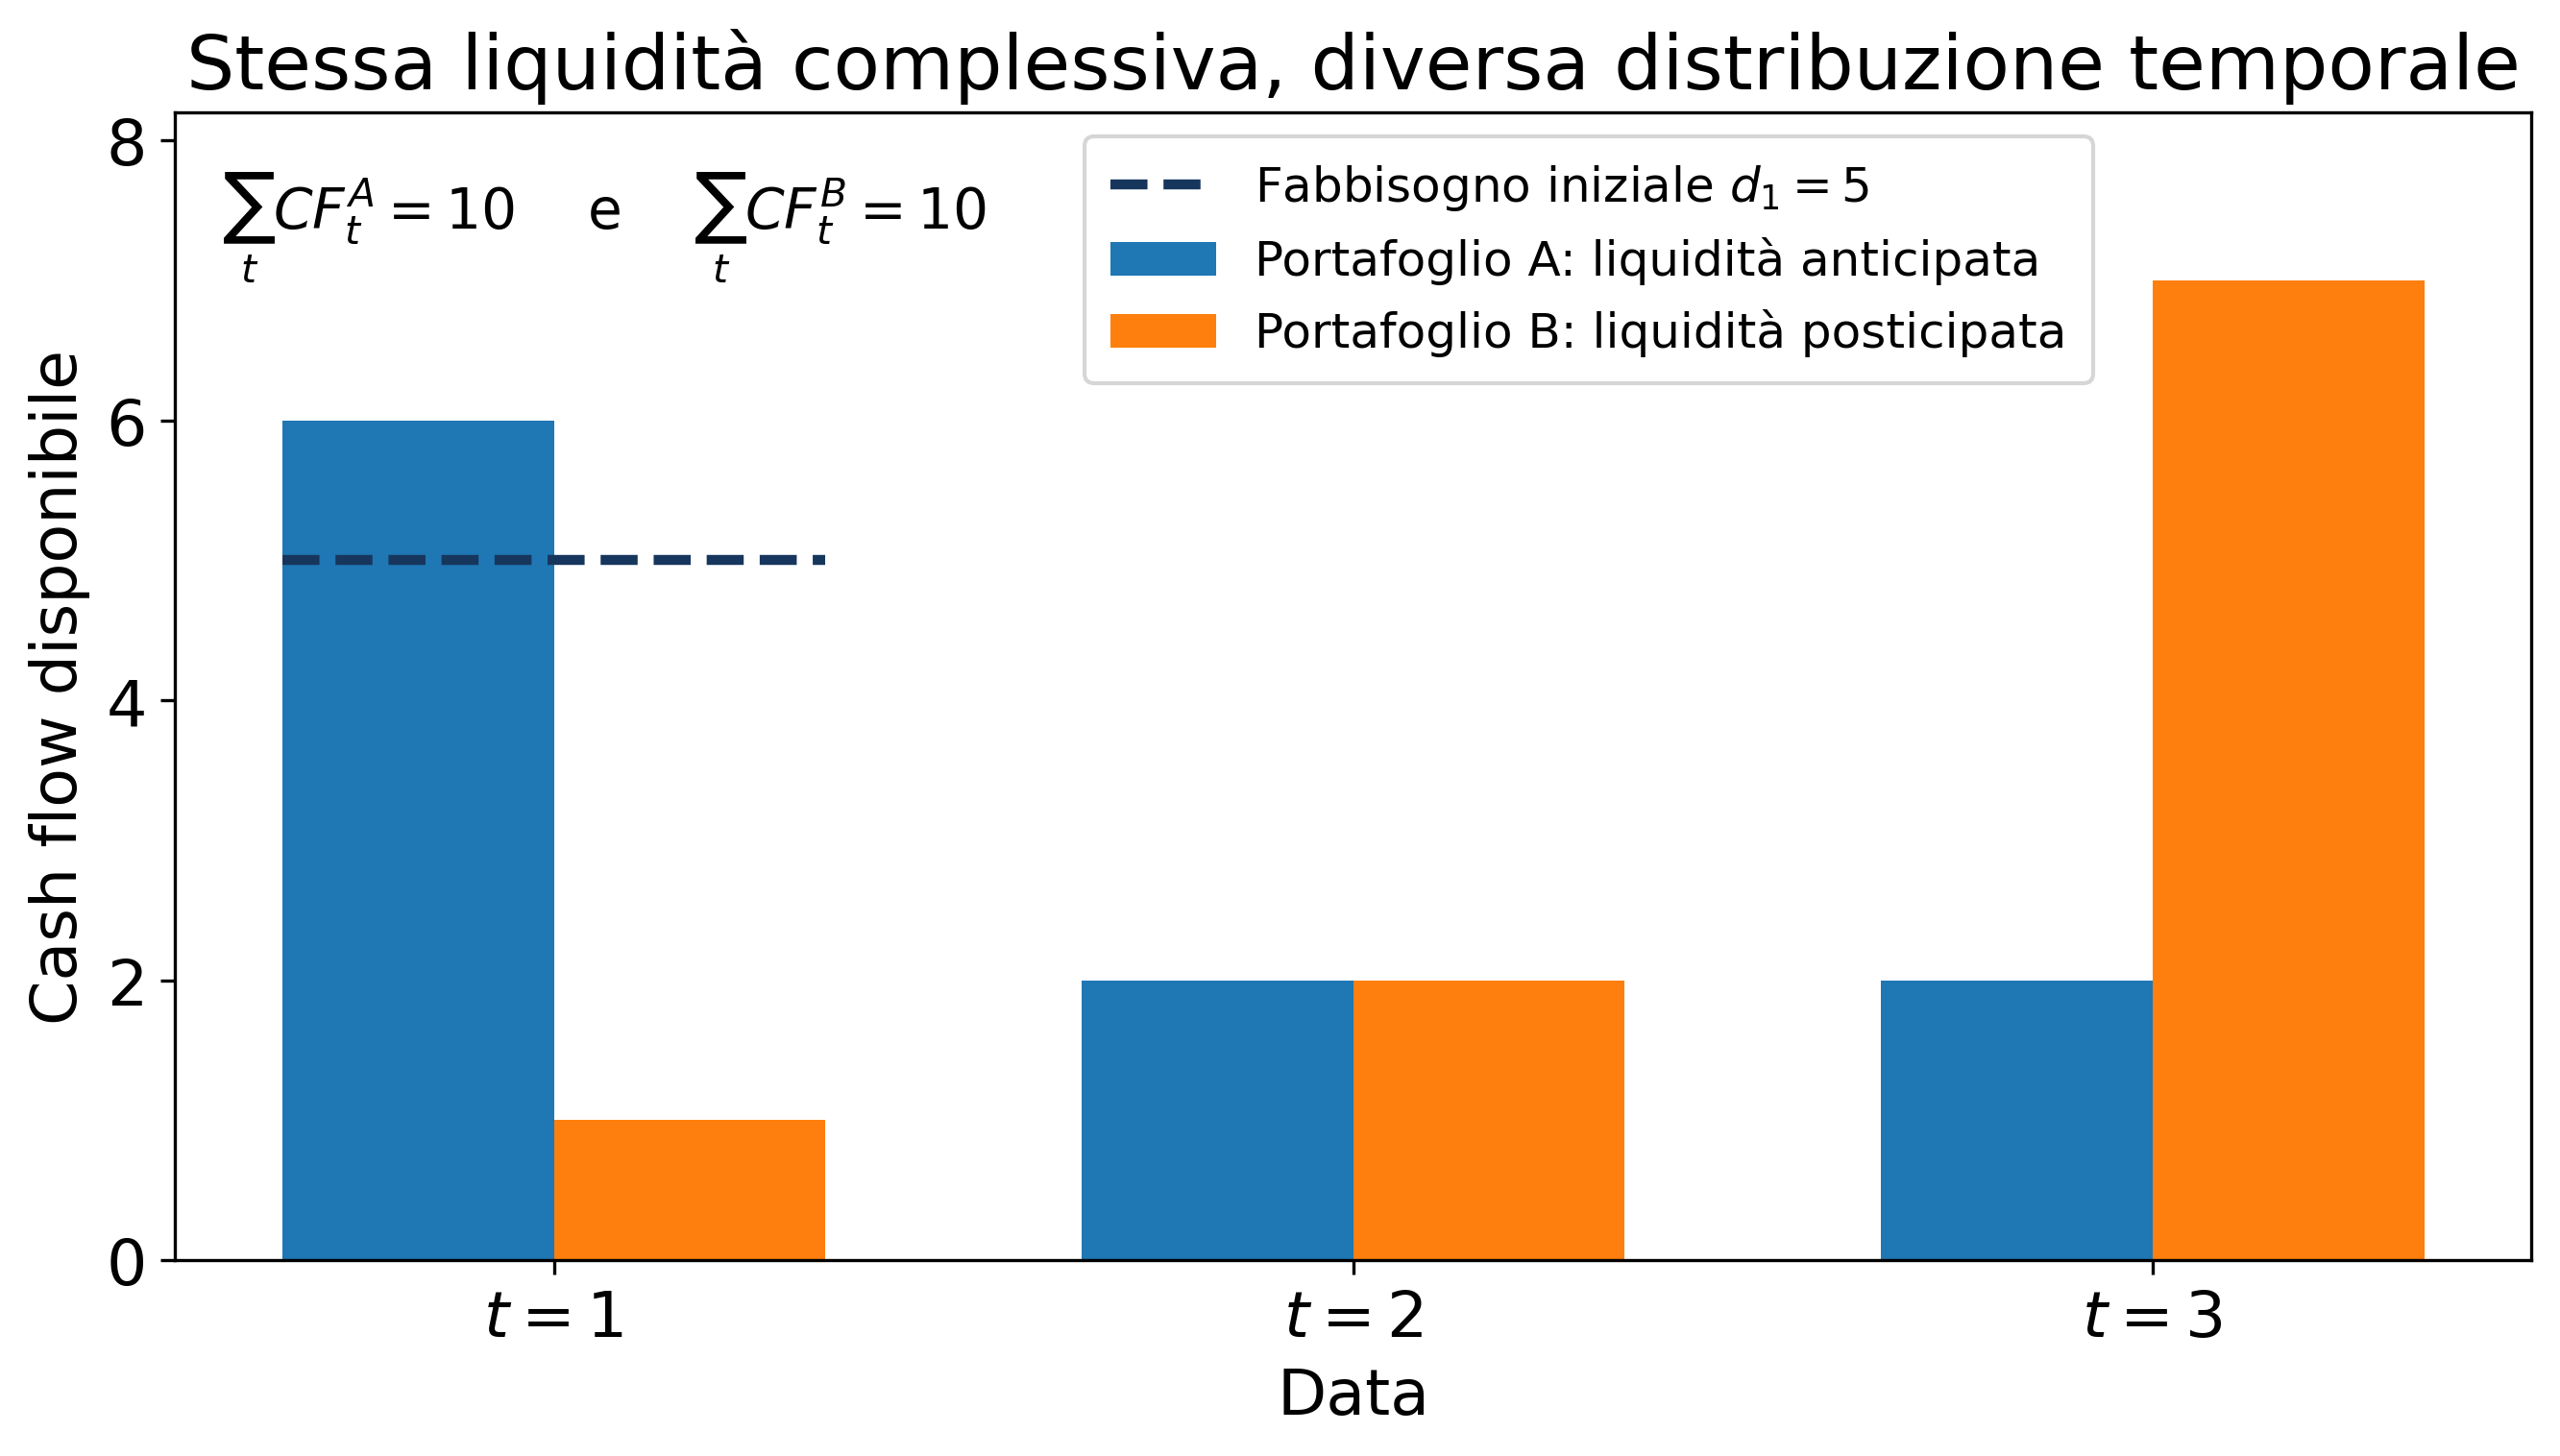
\includegraphics[width=0.90\textwidth]
{../graphics/Cap12_liquidita_aggregata_temporale.png}
\caption{Due portafogli con lo stesso cash flow complessivo ma con diversa
distribuzione temporale. Il portafoglio $A$ produce liquidit\`a in misura
sufficiente a soddisfare il fabbisogno $d_1=5$ alla prima data; il
portafoglio $B$ concentra invece gran parte dei propri flussi alla data
finale.}
\label{fig:cap12-liquidita-aggregata-temporale}
\end{figure}

La Figura~\ref{fig:cap12-liquidita-aggregata-temporale} mostra quindi che la
somma dei cash flow lungo l'intero orizzonte non \`e sufficiente per valutare
la capacit\`a della banca di far fronte ai propri impegni.

La differenza rilevante non riguarda soltanto la quantit\`a complessiva di
liquidit\`a, ma la sua distribuzione nel tempo:

\[
\text{quanto}
\qquad\longrightarrow\qquad
\text{quanto e quando}.
\]

Lo stesso problema si presenta dal lato delle passivit\`a. Una banca non deve
soddisfare un unico fabbisogno aggregato, ma una successione di obblighi,
rimborsi e deflussi collocati in date differenti. La compatibilit\`a tra
attivo e passivo richiede pertanto di confrontare, periodo per periodo, i
flussi prodotti dalle attivit\`a con le risorse richieste dalle passivit\`a.

Introduciamo quindi una sequenza di date

\[
t=0,1,\ldots,T.
\]

Il tempo $t=0$ rappresenta la data nella quale viene scelta la composizione
iniziale del bilancio; le date $t=1,\ldots,T$ rappresentano invece le
scadenze future nelle quali si manifestano cash flow e fabbisogni.

Il problema non consiste pi\`u soltanto nello scegliere una composizione
dell'attivo che soddisfi un requisito complessivo di liquidit\`a. Occorre
scegliere una struttura del bilancio che renda compatibili i flussi generati
dall'attivo con i fabbisogni del passivo lungo l'intero orizzonte temporale.

Il passaggio centrale pu\`o essere sintetizzato come

\[
\boxed{
\text{requisito aggregato di liquidit\`a}
\quad\longrightarrow\quad
\text{bilanci di liquidit\`a alle diverse date}.
}
\]

Questa estensione costituisce il punto di ingresso
nell'Asset--Liability Management deterministico. Il problema resta un
programma lineare: non viene introdotta una nuova classe di ottimizzazione.
Cambiano invece la struttura dei dati e dei vincoli, perch\'e le decisioni
devono ora essere coerenti con una successione di cash flow e fabbisogni
distribuiti nel tempo.

\section{Cash flow degli attivi e fabbisogni alle diverse date}

\label{sec:cap12-cash-flow-fabbisogni}

La sezione precedente ha mostrato che due portafogli con lo stesso cash flow
complessivo possono avere capacit\`a molto diverse di fronteggiare i
fabbisogni della banca. Per rappresentare questa differenza occorre descrivere
separatamente i flussi monetari prodotti alle diverse date.

Consideriamo l'orizzonte discreto

\[
t=0,1,\ldots,T,
\]

e manteniamo il vettore delle decisioni iniziali

\[
x=
\begin{pmatrix}
x_1\\
\vdots\\
x_n
\end{pmatrix},
\]

dove $x_j$ rappresenta l'ammontare destinato alla classe di attivo $j$ al
tempo $0$.

\subsection{Il profilo temporale dei cash flow}

Per ogni attivit\`a $j$ e per ogni data futura $t$, indichiamo con

\[
a_{tj}
\]

il cash flow monetario disponibile alla data $t$ per una unit\`a investita
nell'attivit\`a $j$ al tempo $0$.

L'investimento $x_j$ produce quindi alla data $t$ il flusso

\[
a_{tj}x_j.
\]

Per effetto dell'ipotesi di proporzionalit\`a gi\`a introdotta nel
Capitolo 11, il coefficiente $a_{tj}$ viene trattato come indipendente
dall'ammontare investito. Il cash flow complessivamente prodotto dall'attivo
alla data $t$ \`e pertanto

\[
\sum_{j=1}^{n}a_{tj}x_j.
\]

I coefficienti possono essere raccolti nella matrice dei cash flow

\[
A^{\mathrm{CF}}
=
\begin{pmatrix}
a_{11} & a_{12} & \cdots & a_{1n}\\
a_{21} & a_{22} & \cdots & a_{2n}\\
\vdots & \vdots & \ddots & \vdots\\
a_{T1} & a_{T2} & \cdots & a_{Tn}
\end{pmatrix}.
\]

La matrice $A^{\mathrm{CF}}$ ha $T$ righe e $n$ colonne.

Ogni colonna

\[
\begin{pmatrix}
a_{1j}\\
a_{2j}\\
\vdots\\
a_{Tj}
\end{pmatrix}
\]

descrive il profilo temporale dei cash flow prodotti da una unit\`a della
classe di attivo $j$.

Ogni riga

\[
(a_{t1},\ldots,a_{tn})
\]

descrive invece i cash flow unitari prodotti alla data $t$ dalle diverse
classi di attivo.

Questa organizzazione mantiene la logica matriciale introdotta nel
Capitolo 11. Una colonna continua a descrivere come una variabile decisionale
contribuisce ai diversi requisiti del modello; nel problema multiperiodale,
tali contributi sono ora distinti anche in base alla data nella quale si
manifestano.

\subsection{Il profilo dei fabbisogni}

Dal lato delle passivit\`a, indichiamo con

\[
d_t\geq0
\]

il fabbisogno monetario che deve essere soddisfatto alla data $t$.

La quantit\`a $d_t$ rappresenta l'ammontare di risorse che la banca deve
rendere disponibile in quella data. A seconda della specificazione del
modello, esso pu\`o comprendere rimborsi di passivit\`a, pagamenti
contrattuali, deflussi della raccolta o altri impieghi di liquidit\`a.

Nel modello deterministico sviluppato in questo capitolo, i valori

\[
d_1,d_2,\ldots,d_T
\]

sono trattati come dati noti prima della soluzione del problema e vengono
raccolti nel vettore

\[
d=
\begin{pmatrix}
d_1\\
d_2\\
\vdots\\
d_T
\end{pmatrix}.
\]

La natura deterministica di $d_t$ non implica che i futuri deflussi siano
certi nella realt\`a. Significa che il modello analizza le conseguenze di uno
specifico profilo di fabbisogni assunto come dato nella formulazione
considerata.

Pi\`u avanti il modo in cui tali fabbisogni vengono determinati sar\`a
collegato in modo esplicito alle condizioni economico-finanziarie e alla
situazione patrimoniale della banca. Per il momento, tuttavia, interessa
isolare il problema fondamentale del coordinamento temporale tra risorse
disponibili e risorse richieste.

\begin{figure}[htbp]
\centering
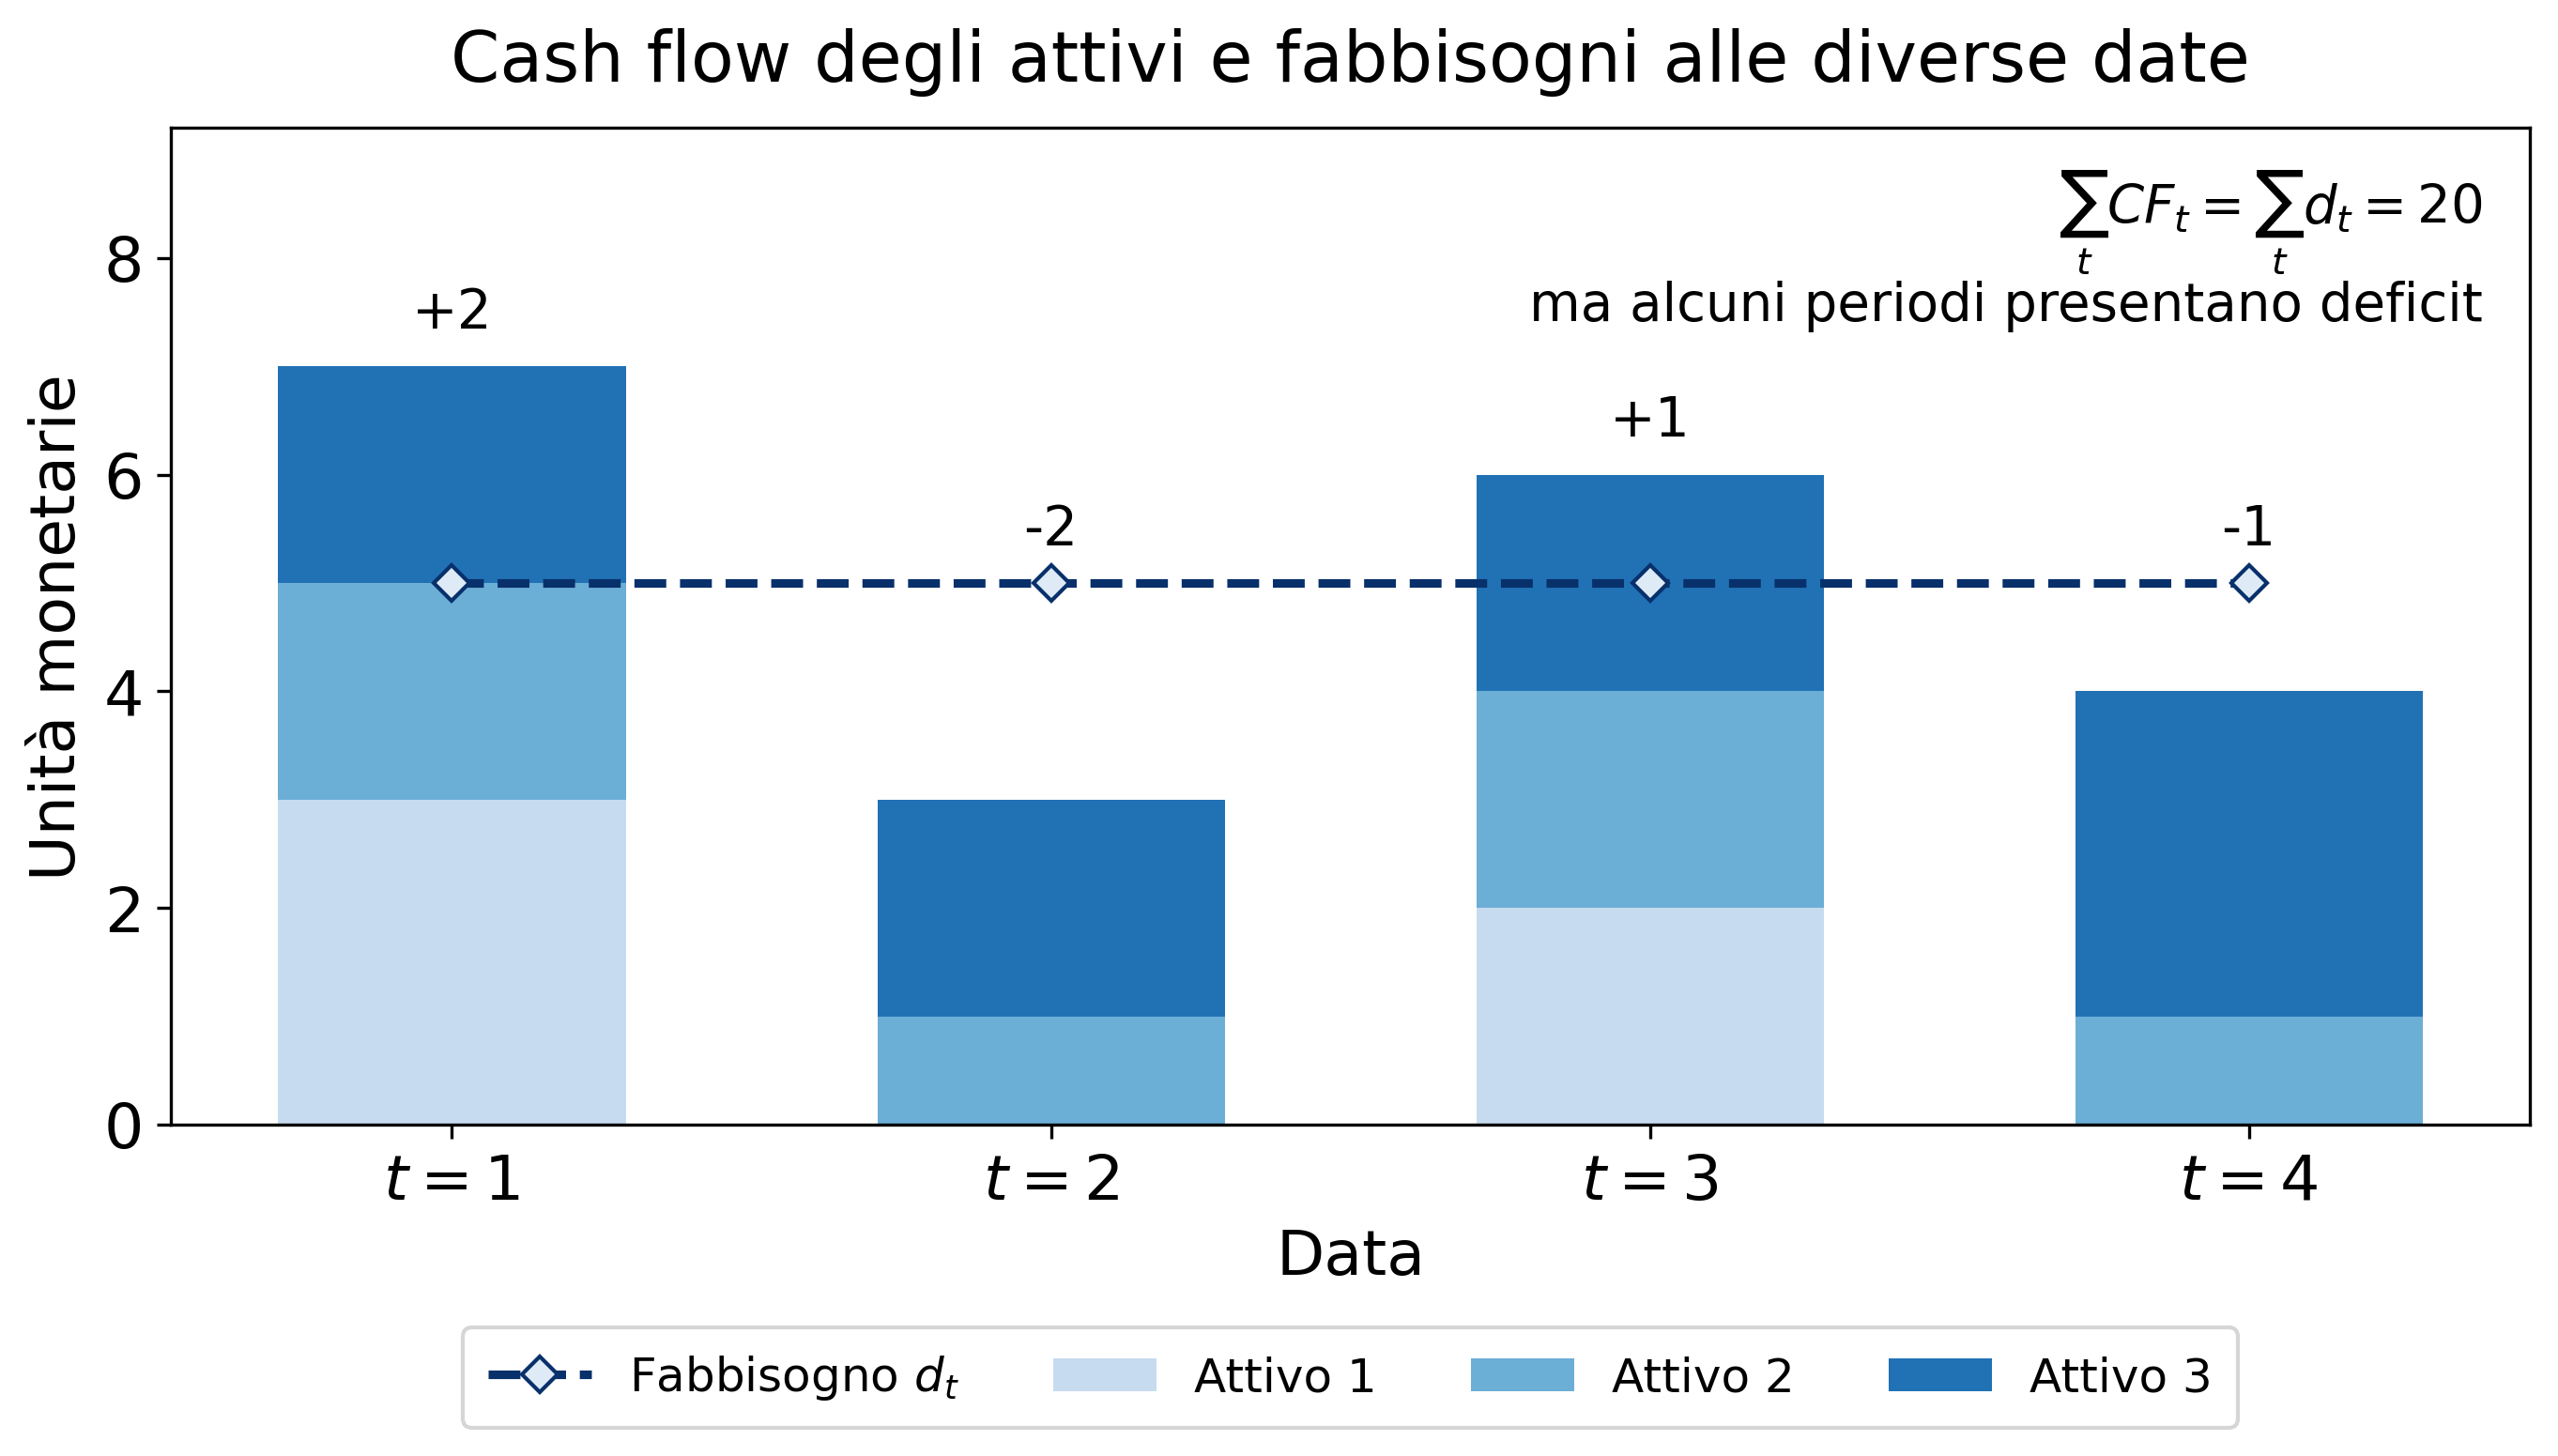
\includegraphics[width=0.92\textwidth]
{../graphics/Cap12_cashflow_attivi_fabbisogni.png}
\caption{Cash flow prodotti dalle diverse classi di attivo e fabbisogni
alle quattro date. Pur coincidendo i cash flow complessivi e i fabbisogni
complessivi sull'intero orizzonte, il profilo temporale presenta surplus
alle date $t=1$ e $t=3$ e deficit alle date $t=2$ e $t=4$.}
\label{fig:cap12-cashflow-fabbisogni}
\end{figure}

La Figura~\ref{fig:cap12-cashflow-fabbisogni} mostra perch\'e il confronto
aggregato non \`e sufficiente. Sull'intero orizzonte le risorse prodotte
dagli attivi coincidono con i fabbisogni:

\[
\sum_{t=1}^{T}CF_t
=
\sum_{t=1}^{T}d_t.
\]

Ci\`o non impedisce tuttavia la presenza di deficit in singole date.
L'Asset--Liability Management deve quindi verificare non soltanto
l'equilibrio complessivo delle risorse, ma la loro disponibilit\`a nel
momento in cui i pagamenti devono essere effettuati.

\subsection{Una prima formulazione: cash-flow matching per data}

Una prima formulazione consiste nel richiedere che, a ciascuna data, i cash
flow prodotti dagli attivi siano almeno sufficienti a coprire il fabbisogno
corrispondente:

\[
\sum_{j=1}^{n}a_{tj}x_j
\geq
d_t,
\qquad
t=1,\ldots,T.
\]

In forma matriciale,

\[
A^{\mathrm{CF}}x
\geq
d.
\]

Il singolo requisito aggregato di liquidit\`a del Capitolo 11 viene quindi
sostituito da $T$ requisiti distinti. La dimensione temporale non viene pi\`u
compressa in un unico coefficiente: per ciascuna data il modello confronta le
risorse monetarie prodotte dall'attivo con il corrispondente fabbisogno.

Questa formulazione rappresenta un primo modello di \emph{cash-flow
matching}. Una composizione dell'attivo \`e ammissibile soltanto se i cash
flow disponibili risultano sufficienti in tutte le date considerate.

Il passaggio dal requisito aggregato

\[
\sum_{j=1}^{n}q_jx_j
\geq
Q_{\min}
\]

ai vincoli

\[
\sum_{j=1}^{n}a_{tj}x_j
\geq
d_t,
\qquad
t=1,\ldots,T,
\]

rende esplicita una differenza fondamentale. Nel primo caso la liquidit\`a
viene misurata come caratteristica complessiva della composizione
dell'attivo; nel secondo viene confrontata con fabbisogni che possiedono una
scadenza precisa.

\subsection{Il limite del matching separato per data}

La formulazione precedente introduce correttamente il tempo, ma considera
ancora ogni data come se fosse indipendente dalle altre.

Supponiamo che, alla data $t$, il portafoglio produca un cash flow superiore
al fabbisogno:

\[
\sum_{j=1}^{n}a_{tj}x_j
>
d_t.
\]

La differenza

\[
\sum_{j=1}^{n}a_{tj}x_j-d_t
\]

rappresenta una disponibilit\`a monetaria residua dopo avere soddisfatto il
fabbisogno della data $t$.

Nei vincoli di cash-flow matching appena formulati, tuttavia, questa
eccedenza non compare nel periodo successivo. Le risorse disponibili alla
data $t$ che non vengono utilizzate scompaiono dal modello e non possono
contribuire alla copertura del fabbisogno alla data $t+1$.

Si tratta di una limitazione economicamente rilevante. Una banca pu\`o
conservare una parte della liquidit\`a disponibile oppure reinvestirla in una
forma compatibile con l'orizzonte successivo. La posizione di liquidit\`a di
una data dipende quindi anche da quanto \`e accaduto nelle date precedenti.

Il problema ALM non pu\`o essere descritto come una semplice successione di
$T$ vincoli indipendenti. Occorre introdurre una variabile che rappresenti la
liquidit\`a residua trasferita da un periodo al successivo.

Il passaggio successivo \`e quindi

\[
\boxed{
\text{cash-flow matching per data}
\quad\longrightarrow\quad
\text{bilanci di liquidit\`a collegati nel tempo}.
}
\]

L'introduzione di questa variabile render\`a esplicita la dipendenza tra il
vincolo relativo alla data $t$ e quello relativo alla data $t+1$ e
costituir\`a il primo vero elemento intertemporale del modello ALM.

\section{Liquidit\`a residua e bilanci intertemporali}

\label{sec:cap12-bilanci-intertemporali}

Il cash-flow matching introdotto nella
Sezione~\ref{sec:cap12-cash-flow-fabbisogni} confronta, per ogni data,
i flussi prodotti dall'attivo con il corrispondente fabbisogno:

\[
\sum_{j=1}^{n}a_{tj}x_j
\geq
d_t,
\qquad
t=1,\ldots,T.
\]

Questa formulazione riconosce che la liquidit\`a deve essere disponibile
nella data in cui viene richiesta, ma non descrive ancora che cosa accade
quando i cash flow prodotti in un periodo superano il fabbisogno dello stesso
periodo.

In una gestione intertemporale, l'eccedenza non scompare. Pu\`o essere
conservata e utilizzata nelle date successive. Per rappresentare questo
meccanismo introduciamo una nuova variabile decisionale.

\begin{definition}[Giacenza di liquidit\`a]

Per ogni data $t=1,\ldots,T$, indichiamo con

\[
g_t\geq0
\]

la liquidit\`a che rimane disponibile immediatamente dopo avere soddisfatto
il fabbisogno $d_t$.

\end{definition}

La variabile $g_t$ \`e quindi uno \emph{stock}, misurato in unit\`a
monetarie. Non rappresenta un nuovo cash flow prodotto dall'attivo, ma la
parte delle risorse disponibili alla data $t$ che non viene utilizzata e
viene trasferita al periodo successivo.

\subsection{Il primo bilancio temporale}

Consideriamo inizialmente la prima data, $t=1$.

I cash flow prodotti dall'attivo sono

\[
\sum_{j=1}^{n}a_{1j}x_j.
\]

Queste risorse devono essere utilizzate per soddisfare il fabbisogno $d_1$;
l'eventuale eccedenza costituisce la giacenza $g_1$.

Il bilancio monetario alla prima data \`e quindi

\[
\sum_{j=1}^{n}a_{1j}x_j
=
d_1+g_1.
\]

La relazione \`e un'uguaglianza, non una disuguaglianza. Tutte le risorse
monetarie disponibili alla data $1$ devono avere una destinazione: una parte
viene utilizzata per soddisfare il fabbisogno, la parte restante viene
conservata come liquidit\`a.

Equivalentemente,

\[
g_1
=
\sum_{j=1}^{n}a_{1j}x_j-d_1.
\]

La condizione

\[
g_1\geq0
\]

garantisce che il fabbisogno della prima data possa essere interamente
soddisfatto.

\subsection{Il collegamento con la data successiva}

Alla data $t=2$ la banca dispone di due fonti di liquidit\`a:

\begin{itemize}

\item i nuovi cash flow prodotti dagli attivi,

\[
\sum_{j=1}^{n}a_{2j}x_j;
\]

\item la giacenza $g_1$ trasferita dalla data precedente.

\end{itemize}

Se, in una prima formulazione, assumiamo che la liquidit\`a trasferita non
produca rendimento, il bilancio alla seconda data diventa

\[
\sum_{j=1}^{n}a_{2j}x_j
+
g_1
=
d_2+g_2.
\]

Pi\`u in generale, per

\[
t=2,\ldots,T,
\]

si ottiene

\[
\sum_{j=1}^{n}a_{tj}x_j
+
g_{t-1}
=
d_t+g_t.
\]

Il sistema completo dei bilanci temporali \`e pertanto

\[
\begin{array}{rcl}
\displaystyle
\sum_{j=1}^{n}a_{1j}x_j
-
g_1
&=&
d_1,
\\[8pt]
\displaystyle
\sum_{j=1}^{n}a_{2j}x_j
+
g_1-g_2
&=&
d_2,
\\
&\vdots&
\\
\displaystyle
\sum_{j=1}^{n}a_{Tj}x_j
+
g_{T-1}-g_T
&=&
d_T.
\end{array}
\]

La differenza rispetto al cash-flow matching separato per data \`e
fondamentale. La variabile $g_t$ compare contemporaneamente nel bilancio
della data $t$ e in quello della data $t+1$.

Il vincolo relativo a una data non pu\`o quindi pi\`u essere interpretato
isolatamente:

\[
\boxed{
g_t
\text{ collega il bilancio della data }t
\text{ al bilancio della data }t+1.
}
\]

Questa \`e la struttura intertemporale essenziale del modello.

\subsection{La liquidit\`a come variabile di stato}

La giacenza $g_t$ possiede una funzione diversa dalle variabili iniziali
$x_j$.

Le quantit\`a

\[
x_1,\ldots,x_n
\]

determinano la composizione dell'attivo \textbf{scelta} al tempo $0$.

La quantit\`a

\[
g_t
\]

descrive invece la posizione di liquidit\`a con la quale la banca conclude la
data $t$ e affronta la data successiva.

In questo senso, $g_t$ pu\`o essere interpretata come una semplice
\emph{variabile di stato}: sintetizza una conseguenza delle decisioni e dei
cash flow passati che diventa rilevante per i vincoli futuri.

Dal bilancio temporale segue infatti la relazione ricorsiva

\[
g_t
=
g_{t-1}
+
\sum_{j=1}^{n}a_{tj}x_j
-
d_t,
\qquad
t=1,\ldots,T,
\]

ponendo per il momento

\[
g_0=0.
\]

La liquidit\`a disponibile alla fine di ogni data dipende quindi dalla
liquidit\`a ereditata dal periodo precedente, dai nuovi flussi prodotti
dall'attivo e dal fabbisogno corrente.

Questa rappresentazione rende esplicito un principio centrale
dell'Asset--Liability Management:

\[
\boxed{
\begin{array}{c}
\text{la posizione finanziaria a una data dipende anche}\\
\text{dalle decisioni e dai saldi accumulati nelle date precedenti}
\end{array}
}
\]

\subsection{Il rendimento della liquidit\`a trasferita}

L'ipotesi secondo cui la liquidit\`a trasferita da una data alla successiva
mantenga invariato il proprio valore \`e utile per isolare la struttura dei
bilanci, ma pu\`o essere raffinata.

Supponiamo che la giacenza disponibile dopo la data $t-1$ possa essere
impiegata fino alla data $t$ a un tasso deterministico $r_{t-1}$.

Una unit\`a monetaria detenuta alla fine della data $t-1$ diventa quindi

\[
1+r_{t-1}
\]

unit\`a alla data $t$.

Per $t=2,\ldots,T$, il bilancio diventa

\[
\sum_{j=1}^{n}a_{tj}x_j
+
(1+r_{t-1})g_{t-1}
=
d_t+g_t.
\]

Per la prima data resta

\[
\sum_{j=1}^{n}a_{1j}x_j
=
d_1+g_1,
\]

se si assume che non esista una giacenza iniziale separata dalla composizione
$x$ scelta al tempo $0$.

Il sistema pu\`o quindi essere scritto come

\[
\begin{array}{rcl}
\displaystyle
\sum_{j=1}^{n}a_{1j}x_j-g_1
&=&
d_1,
\\[8pt]
\displaystyle
\sum_{j=1}^{n}a_{2j}x_j
+
(1+r_1)g_1-g_2
&=&
d_2,
\\
&\vdots&
\\
\displaystyle
\sum_{j=1}^{n}a_{Tj}x_j
+
(1+r_{T-1})g_{T-1}-g_T
&=&
d_T.
\end{array}
\]

Il coefficiente $1+r_{t-1}$ non modifica la natura lineare del modello,
poich\'e il tasso $r_{t-1}$ \`e trattato come un dato deterministico.

\subsection{Condizione finale}

La variabile $g_T$ rappresenta la liquidit\`a residua alla fine
dell'orizzonte considerato. Il suo trattamento dipende dalla funzione del
modello.

Se l'orizzonte termina quando tutti gli obblighi rilevanti sono stati
soddisfatti e non si attribuisce valore alla liquidit\`a residua, pu\`o essere
imposta la condizione

\[
g_T=0.
\]

Se invece la liquidit\`a finale rappresenta una risorsa economicamente utile
oltre l'orizzonte del modello, essa non deve essere forzata a zero: dovr\`a
essere mantenuta come variabile oppure valorizzata nella funzione obiettivo.

La condizione terminale non \`e quindi un dettaglio tecnico. Stabilisce che
cosa il modello considera economicamente rilevante al termine
dell'orizzonte.

\subsection{Dal matching al bilancio dinamico}

Il passaggio compiuto in questa sezione pu\`o essere riassunto confrontando le
due formulazioni.

Nel cash-flow matching separato per data:

\[
\sum_{j=1}^{n}a_{tj}x_j
\geq
d_t.
\]

Nel modello con trasferimento della liquidit\`a:

\[
\sum_{j=1}^{n}a_{tj}x_j
+
(1+r_{t-1})g_{t-1}
=
d_t+g_t.
\]

Nel primo caso ciascuna data costituisce un confronto autonomo tra flussi e
fabbisogni. Nel secondo, il saldo di un periodo diventa una risorsa del
periodo successivo.

La programmazione rimane lineare, ma la struttura economica del problema
cambia profondamente: il modello non confronta pi\`u soltanto attivit\`a e
passivit\`a alle singole date, bens\`i descrive l'evoluzione nel tempo della
posizione di liquidit\`a della banca.

Questo collegamento prepara il passo successivo. La liquidit\`a accumulata
internamente non \`e infatti l'unico strumento con cui una banca pu\`o
fronteggiare un fabbisogno temporaneo. Quando i cash flow dell'attivo e la
giacenza disponibile non sono sufficienti, la banca pu\`o ricorrere a
funding esterno. Tale scelta produce liquidit\`a nella data corrente, ma
genera contemporaneamente un obbligo di rimborso futuro.

\section{Funding esterno e obblighi di rimborso}

\label{sec:cap12-funding}

I bilanci intertemporali introdotti nella
Sezione~\ref{sec:cap12-bilanci-intertemporali} assumono che la banca possa
soddisfare i propri fabbisogni utilizzando esclusivamente i cash flow prodotti
dall'attivo e la liquidit\`a accumulata nelle date precedenti.

Questa rappresentazione mette in evidenza il collegamento temporale tra le
diverse date, ma trascura una possibilit\`a importante. Se le risorse interne
non sono sufficienti a soddisfare un fabbisogno corrente, la banca pu\`o
ricorrere a una fonte esterna di funding.

Il funding modifica la disponibilit\`a di liquidit\`a nella data in cui viene
raccolto, ma non costituisce una risorsa gratuita. Le somme ottenute devono
essere rimborsate in una data successiva insieme al relativo costo
finanziario.

\subsection{Una fonte di funding a un periodo}

Per mantenere leggibile la struttura del modello, consideriamo una sola forma
stilizzata di funding con durata pari a un periodo.

Per

\[
t=1,\ldots,T-1,
\]

indichiamo con

\[
u_t\geq0
\]

l'ammontare di funding raccolto alla data $t$.

La quantit\`a $u_t$ \`e immediatamente disponibile e pu\`o quindi essere
utilizzata per soddisfare il fabbisogno della stessa data.

Supponiamo che il funding raccolto alla data $t$ debba essere rimborsato alla
data $t+1$ a un tasso deterministico $\rho_t$. L'obbligo di rimborso generato
da $u_t$ \`e pertanto

\[
(1+\rho_t)u_t.
\]

La sequenza economica \`e quindi

\[
\boxed{
\begin{array}{c}
\text{funding raccolto alla data }t:\quad u_t\\[3pt]
\downarrow\\[3pt]
\text{liquidit\`a disponibile alla data }t\\[3pt]
\downarrow\\[3pt]
\text{rimborso alla data }t+1:\quad (1+\rho_t)u_t
\end{array}
}
\]

Il funding trasferisce quindi risorse dalla data futura alla data corrente:
aumenta la liquidit\`a disponibile oggi, ma riduce quella disponibile domani.

\subsection{Il bilancio alla prima data}

Alla data $t=1$ la banca dispone dei cash flow prodotti dagli attivi,

\[
\sum_{j=1}^{n}a_{1j}x_j,
\]

e pu\`o inoltre raccogliere funding per un ammontare $u_1$.

Le risorse vengono utilizzate per soddisfare il fabbisogno $d_1$ e
l'eventuale eccedenza viene mantenuta come giacenza $g_1$.

Il bilancio diventa quindi

\[
\sum_{j=1}^{n}a_{1j}x_j
+
u_1
=
d_1+g_1.
\]

Rispetto alla formulazione della sezione precedente, il termine $u_1$
costituisce una nuova fonte di liquidit\`a.

Il suo utilizzo produce tuttavia un effetto sul periodo successivo.

\subsection{Il bilancio nelle date intermedie}

Consideriamo una generica data

\[
t=2,\ldots,T-1.
\]

Le risorse disponibili sono ora costituite da tre componenti:

\begin{itemize}

\item i cash flow prodotti dagli attivi,

\[
\sum_{j=1}^{n}a_{tj}x_j;
\]

\item la giacenza proveniente dalla data precedente, capitalizzata al tasso
$r_{t-1}$,

\[
(1+r_{t-1})g_{t-1};
\]

\item il nuovo funding raccolto alla data corrente,

\[
u_t.
\]

\end{itemize}

A queste risorse si contrappongono tre utilizzi:

\begin{itemize}

\item il fabbisogno corrente $d_t$;

\item il rimborso del funding raccolto alla data precedente,

\[
(1+\rho_{t-1})u_{t-1};
\]

\item la nuova giacenza di liquidit\`a $g_t$.

\end{itemize}

Il bilancio intertemporale completo \`e quindi

\[
\sum_{j=1}^{n}a_{tj}x_j
+
(1+r_{t-1})g_{t-1}
+
u_t
=
d_t
+
(1+\rho_{t-1})u_{t-1}
+
g_t.
\]

La stessa variabile $u_t$ svolge quindi due ruoli in date consecutive:

\[
u_t
\]

\`e una risorsa nel bilancio della data $t$, mentre

\[
(1+\rho_t)u_t
\]

diventa un utilizzo nel bilancio della data $t+1$.

Il funding introduce cos\`i un secondo collegamento intertemporale, accanto a
quello gi\`a prodotto dalla giacenza $g_t$.

\begin{figure}[htbp]
\centering
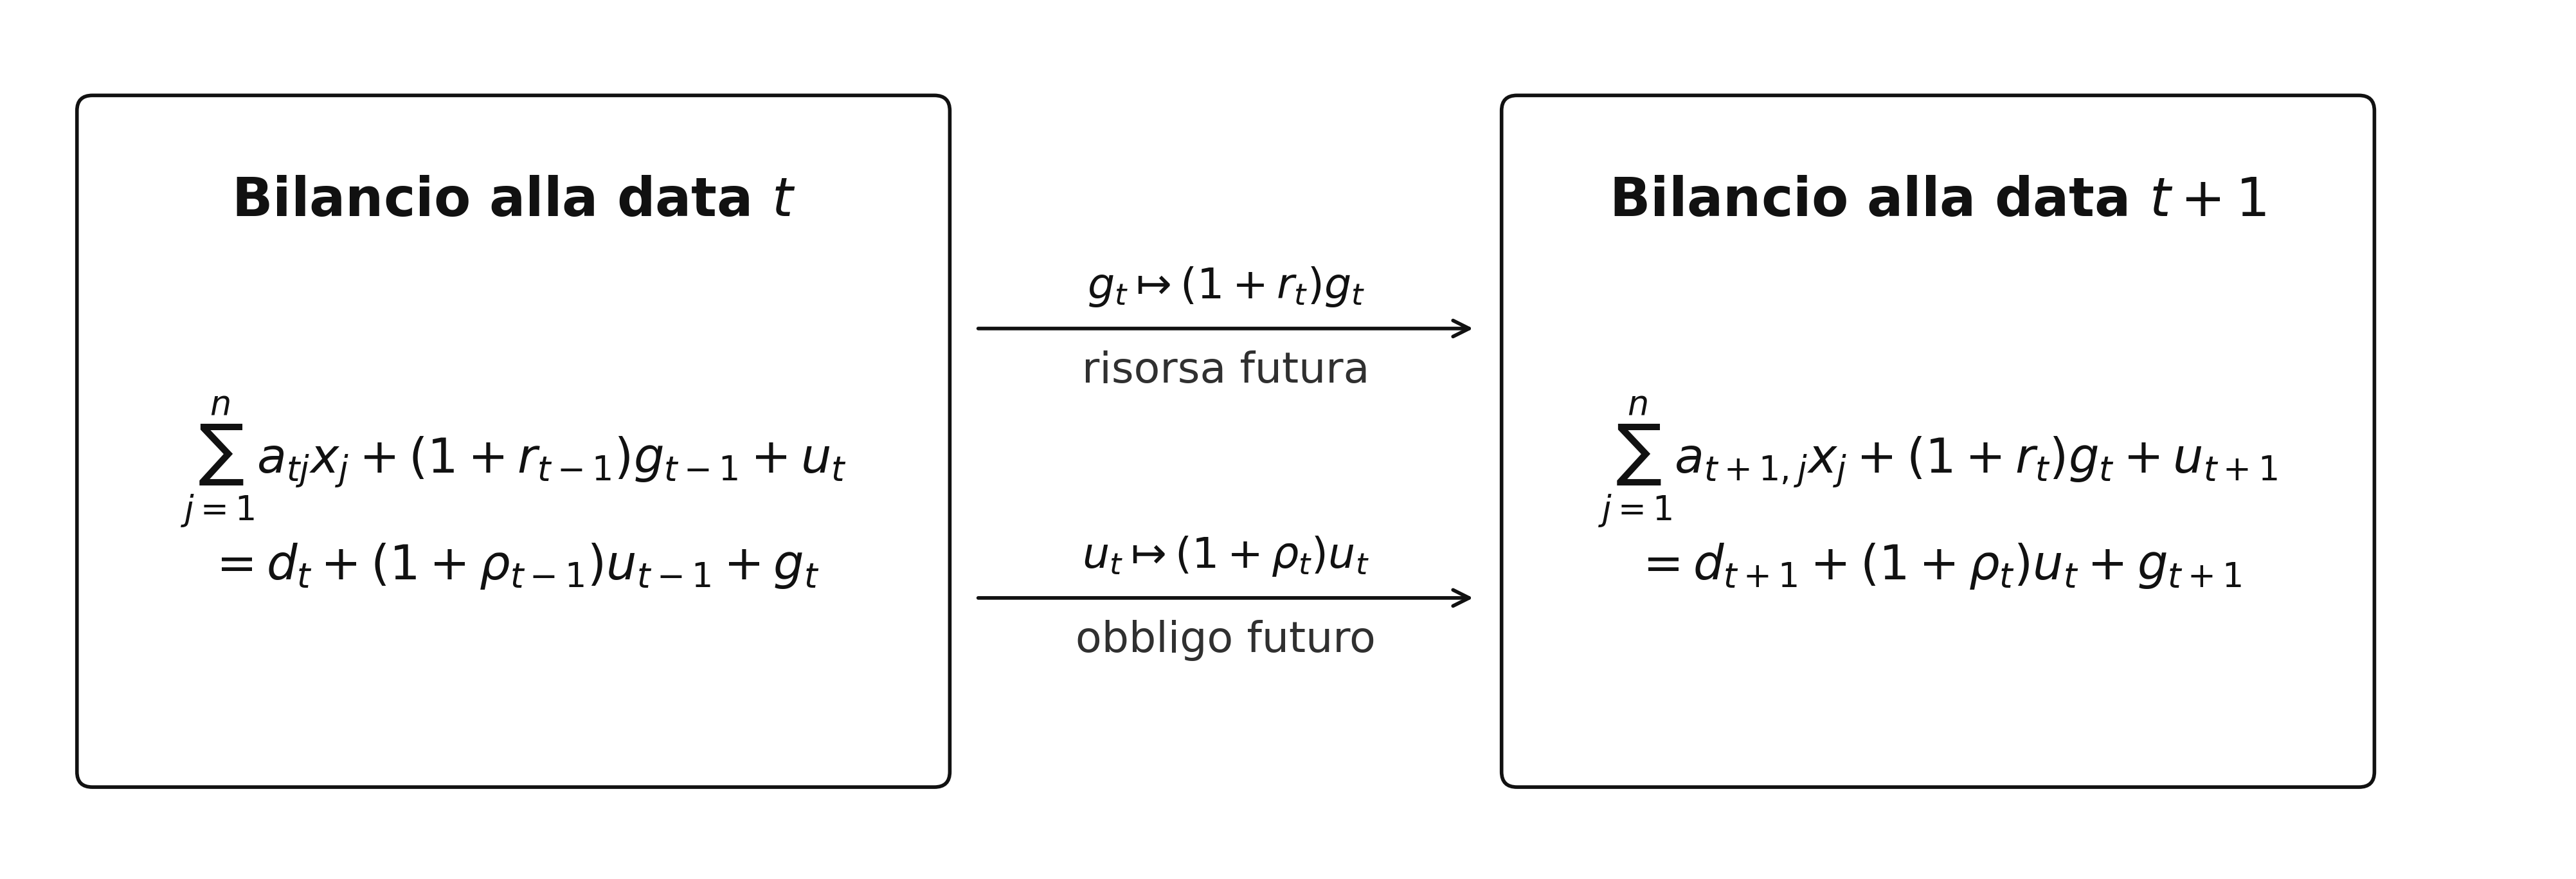
\includegraphics[width=0.96\textwidth]
{../graphics/Cap12_bilancio_intertemporale.png}
\caption{Collegamento tra due bilanci di liquidit\`a consecutivi. La
giacenza $g_t$ costituisce una risorsa disponibile alla data successiva,
mentre il funding $u_t$ raccolto alla data corrente genera un obbligo di
rimborso pari a $(1+\rho_t)u_t$ alla data successiva.}
\label{fig:cap12-bilancio-intertemporale}
\end{figure}

La Figura~\ref{fig:cap12-bilancio-intertemporale} rende visibili i due
collegamenti fondamentali tra date consecutive. La giacenza trasferisce
risorse verso il futuro; il funding trasferisce invece risorse dal futuro
al presente e genera per questo un successivo obbligo di rimborso.

Le due variabili hanno quindi effetti temporali opposti:

\[
g_t
\quad\text{accumula una risorsa per il periodo successivo},
\]

mentre

\[
u_t
\quad\text{anticipa una risorsa creando un'obbligazione futura}.
\]

La struttura intertemporale del modello nasce precisamente dalla presenza
simultanea di questi collegamenti.

\subsection{Il bilancio alla data finale}

Alla data finale $T$ non introduciamo nuovo funding. Questa scelta garantisce
che ogni posizione di funding aperta all'interno dell'orizzonte venga anche
rimborsata entro l'orizzonte stesso.

Il bilancio finale \`e pertanto

\[
\sum_{j=1}^{n}a_{Tj}x_j
+
(1+r_{T-1})g_{T-1}
=
d_T
+
(1+\rho_{T-1})u_{T-1}
+
g_T.
\]

Il sistema completo pu\`o quindi essere scritto come

\[
\begin{array}{rcl}
\displaystyle
\sum_{j=1}^{n}a_{1j}x_j+u_1-g_1
&=&
d_1,
\\[8pt]
\displaystyle
\sum_{j=1}^{n}a_{tj}x_j
+
(1+r_{t-1})g_{t-1}
+
u_t
-
(1+\rho_{t-1})u_{t-1}
-
g_t
&=&
d_t,
\\
&&
t=2,\ldots,T-1,
\\[8pt]
\displaystyle
\sum_{j=1}^{n}a_{Tj}x_j
+
(1+r_{T-1})g_{T-1}
-
(1+\rho_{T-1})u_{T-1}
-
g_T
&=&
d_T.
\end{array}
\]

Le condizioni di non negativit\`a sono

\[
g_t\geq0,
\qquad
t=1,\ldots,T,
\]

e

\[
u_t\geq0,
\qquad
t=1,\ldots,T-1.
\]

\subsection{Limiti alla disponibilit\`a di funding}

La possibilit\`a di raccogliere funding non pu\`o essere considerata
illimitata.

Introduciamo pertanto, per ogni data,

\[
\bar{u}_t\geq0,
\]

che rappresenta l'ammontare massimo di funding accessibile alla banca.

Il vincolo

\[
0\leq u_t\leq\bar{u}_t,
\qquad
t=1,\ldots,T-1,
\]

pu\`o riflettere limiti contrattuali, capacit\`a di accesso al mercato,
disponibilit\`a di linee di credito o altri vincoli sulla raccolta
incrementale.

Il parametro $\bar{u}_t$ ha un significato diverso da $u_t$:

\[
u_t
=
\text{decisione di funding},
\]

mentre

\[
\bar{u}_t
=
\text{massima capacit\`a di funding disponibile}.
\]

La banca decide quindi quanto funding utilizzare all'interno di una
capacit\`a data.

\subsection{Costo del funding e assenza di arbitraggio artificiale}

Il tasso $\rho_t$ rappresenta il costo complessivo della fonte di funding
utilizzata tra le date $t$ e $t+1$.

Nello stesso intervallo, la giacenza di liquidit\`a produce il rendimento
$r_t$.

Per evitare che il modello trovi conveniente raccogliere funding unicamente
per investirlo nella giacenza di liquidit\`a, \`e naturale assumere

\[
\rho_t\geq r_t.
\]

In una rappresentazione bancaria realistica ci si attende normalmente

\[
\rho_t>r_t,
\]

poich\'e la raccolta esterna incorpora un costo superiore al rendimento di una
posizione liquida priva di rischio comparabile.

La differenza

\[
\rho_t-r_t
\]

rappresenta quindi, in forma stilizzata, il costo aggiuntivo associato
all'accesso al funding.

Questa condizione non \`e necessaria per la linearit\`a matematica del
problema, ma evita un comportamento economicamente artificiale del modello.

\subsection{Funding e gestione della liquidit\`a}

L'introduzione di $u_t$ modifica il significato del problema ALM.

Senza funding, un'insufficienza dei cash flow e della liquidit\`a accumulata
rende il piano non ammissibile.

Con il funding, la banca dispone di una seconda possibilit\`a:

\[
\text{deficit corrente}
\quad\longrightarrow\quad
\text{funding oggi}
\quad\longrightarrow\quad
\text{obbligo di rimborso domani}.
\]

Il funding non elimina quindi il problema della liquidit\`a. Ne modifica la
distribuzione temporale.

Una scelta di funding che risolve un deficit alla data $t$ pu\`o infatti
rendere pi\`u difficile soddisfare il bilancio alla data $t+1$, a causa del
rimborso

\[
(1+\rho_t)u_t.
\]

La decisione non pu\`o pertanto essere valutata considerando esclusivamente il
periodo corrente.

Il modello comincia cos\`i a rappresentare il nucleo dell'Asset--Liability
Management:

\[
\boxed{
\begin{array}{c}
\text{le risorse disponibili oggi dipendono dalle decisioni passate,}\\
\text{mentre le decisioni assunte oggi modificano i fabbisogni futuri.}
\end{array}
}
\]

La struttura resta interamente lineare. I coefficienti $a_{tj}$, $d_t$,
$r_t$, $\rho_t$ e $\bar{u}_t$ sono, in questa fase, dati deterministici;
$x_j$, $g_t$ e $u_t$ sono invece le variabili attraverso le quali il modello
descrive la composizione dell'attivo e la gestione intertemporale della
liquidit\`a.

La sezione successiva preciser\`a come tali coefficienti possano essere
ricondotti a un ambiente economico-finanziario deterministico e come il
modello ALM possa essere collegato in modo coerente al caso bancario
sviluppato nel Capitolo 11.

\section{L'ambiente economico-finanziario deterministico}

\label{sec:cap12-ambiente-deterministico}

Le sezioni precedenti hanno costruito la struttura intertemporale del modello
ALM. I cash flow degli attivi, la giacenza di liquidit\`a e il funding
collegano le diverse date attraverso i bilanci

\[
\sum_{j=1}^{n}a_{tj}x_j
+
(1+r_{t-1})g_{t-1}
+
u_t
=
d_t
+
(1+\rho_{t-1})u_{t-1}
+
g_t.
\]

Finora i coefficienti

\[
a_{tj},\qquad r_t,\qquad \rho_t,\qquad \bar{u}_t
\]

sono stati trattati semplicemente come dati del modello. In un problema
bancario, tuttavia, tali coefficienti riflettono le condizioni
economico-finanziarie nelle quali la banca opera.

Per rendere esplicito questo collegamento introduciamo, per ogni data
$t=0,1,\ldots,T$, il vettore

\[
\bar{Z}_t
=
\left(
\bar{R}_t,\bar{C}_t,\bar{F}_t
\right).
\]

La barra indica che, nel presente capitolo, l'intera traiettoria

\[
\bar{Z}_0,\bar{Z}_1,\ldots,\bar{Z}_T
\]

\`e considerata nota al momento della formulazione del problema.

Il modello \`e quindi deterministico, ma i valori dei fattori possono variare
nel tempo:

\[
\bar{Z}_t
\neq
\bar{Z}_{t+1}.
\]

La caratteristica deterministica riguarda la conoscenza della traiettoria,
non la sua costanza.

\subsection{Tre dimensioni dell'ambiente finanziario}

Le tre componenti di $\bar{Z}_t$ hanno funzioni economiche distinte.

Il fattore

\[
\bar{R}_t
\]

rappresenta il livello dei tassi privi di rischio rilevante nell'intervallo
considerato. Esso pu\`o essere interpretato come il \emph{prezzo del tempo}:
determina il rendimento delle disponibilit\`a liquide e contribuisce alla
valutazione dei flussi monetari distribuiti nel tempo.

Il fattore

\[
\bar{C}_t
\]

rappresenta il livello dello spread di credito osservato sul mercato. Esso
misura il premio richiesto per detenere esposizioni soggette a rischio di
credito e pu\`o essere interpretato come il \emph{prezzo del rischio di
credito}.

Il fattore

\[
\bar{F}_t
\]

rappresenta invece lo spread o la tensione associata al funding della banca.
Esso misura quanto l'accesso alla raccolta esterna sia costoso o difficile
rispetto a una fonte priva di rischio comparabile e pu\`o essere interpretato
come il \emph{prezzo della scarsit\`a di funding}.

La distinzione pu\`o essere sintetizzata come

\[
\boxed{
\begin{array}{c}
\bar{R}_t:\ \text{prezzo del tempo},\\[3pt]
\bar{C}_t:\ \text{prezzo del rischio di credito},\\[3pt]
\bar{F}_t:\ \text{prezzo della scarsit\`a di funding}.
\end{array}
}
\]

I tre fattori descrivono l'ambiente esterno nel quale la banca opera. Non
dipendono dalle decisioni $x_j$, $g_t$ o $u_t$ assunte nel modello.

\subsection{Dal livello dei tassi al rendimento della liquidit\`a}

Nella Sezione~\ref{sec:cap12-bilanci-intertemporali} il parametro $r_t$
rappresenta il rendimento ottenibile mantenendo una giacenza di liquidit\`a
tra le date $t$ e $t+1$.

Il suo valore pu\`o essere ricondotto al livello del tasso privo di rischio:

\[
r_t
=
r(\bar{R}_t).
\]

Nella rappresentazione pi\`u semplice, se $\bar{R}_t$ indica direttamente il
tasso applicabile alla giacenza nell'intervallo considerato, si pu\`o porre

\[
r_t=\bar{R}_t.
\]

Il bilancio utilizza quindi

\[
(1+\bar{R}_t)g_t
\]

come ammontare disponibile alla data successiva.

La relazione non deve essere interpretata come una legge generale di mercato.
Essa costituisce una specificazione coerente con un modello nel quale la
liquidit\`a residua viene investita per un periodo in una forma a rischio
trascurabile.

\subsection{Il costo del funding}

Il tasso $\rho_t$ introdotto nella
Sezione~\ref{sec:cap12-funding} rappresenta invece il costo del funding
raccolto alla data $t$ e rimborsato alla data $t+1$.

Il suo valore dipende sia dal livello generale dei tassi sia dalle condizioni
specifiche di funding della banca. Una rappresentazione naturale \`e

\[
\rho_t
=
\rho(\bar{R}_t,\bar{F}_t).
\]

Se $\bar{F}_t$ viene misurato direttamente come spread sul tasso privo di
rischio, una specificazione particolarmente semplice \`e

\[
\rho_t
=
\bar{R}_t+\bar{F}_t.
\]

Il rimborso del funding diventa quindi

\[
\left(
1+\bar{R}_t+\bar{F}_t
\right)u_t.
\]

Questa rappresentazione rende esplicita la differenza tra il rendimento della
liquidit\`a e il costo della raccolta esterna. Se

\[
\bar{F}_t>0,
\]

allora

\[
\rho_t>r_t,
\]

coerentemente con l'ipotesi introdotta nella sezione precedente.

Il funding \`e quindi tanto pi\`u costoso quanto maggiore \`e la tensione
associata alla raccolta della banca.

\subsection{Disponibilit\`a di funding}

Le condizioni di funding possono incidere non soltanto sul costo della
raccolta, ma anche sull'ammontare massimo accessibile.

Il parametro

\[
\bar{u}_t
\]

rappresenta la capacit\`a massima di funding disponibile alla data $t$.

In forma generale si pu\`o scrivere

\[
\bar{u}_t
=
\bar{u}(\bar{F}_t).
\]

In condizioni di funding favorevoli la banca pu\`o disporre di una maggiore
capacit\`a di raccolta; in condizioni di stress tale capacit\`a pu\`o
ridursi.

Non \`e necessario specificare in questa fase una particolare forma
funzionale. Nel problema deterministico, una volta fissata la traiettoria
$\bar{F}_t$, anche

\[
\bar{u}_1,\ldots,\bar{u}_{T-1}
\]

sono coefficienti noti.

Il vincolo

\[
0\leq u_t\leq\bar{u}_t
\]

rimane pertanto lineare.

\subsection{Il ruolo dello spread di credito}

Il fattore $\bar{C}_t$ richiede una precisazione particolare.

Se un'attivit\`a produce cash flow contrattuali certi e viene mantenuta fino
alla scadenza, una variazione dello spread di credito di mercato non modifica
automaticamente tali cash flow.

Non sarebbe quindi corretto introdurre $\bar{C}_t$ nei coefficienti
$a_{tj}$ per il solo fatto che il modello contiene un fattore di credito.

Il fattore $\bar{C}_t$ diventa invece rilevante quando i flussi disponibili
per l'ALM dipendono dalla qualit\`a creditizia o dal valore economico delle
attivit\`a. Ci\`o pu\`o accadere, per esempio, quando il modello considera:

\begin{itemize}

\item cash flow corretti per perdite creditizie;

\item valori di realizzo di titoli o prestiti;

\item haircuts applicati alle attivit\`a utilizzate per ottenere liquidit\`a;

\item valori di mercato di esposizioni creditizie.

\end{itemize}

In tali casi i coefficienti dei cash flow possono essere scritti, in forma
generale, come

\[
a_{tj}
=
a_{tj}
\left(
\bar{R}_t,\bar{C}_t
\right),
\]

per le classi di attivo sensibili a tali fattori.

Per altre attivit\`a, invece, la dipendenza da $\bar{C}_t$ pu\`o essere
assente.

Questa distinzione \`e importante: non tutti i fattori economici devono
entrare in tutti i coefficienti del modello.

\subsection{Fattori esterni e coefficienti del modello}

La relazione tra ambiente esterno e parametri ALM pu\`o essere sintetizzata
come

\[
\bar{Z}_t
=
(\bar{R}_t,\bar{C}_t,\bar{F}_t)
\quad\longrightarrow\quad
\left\{
a_{tj},\,
r_t,\,
\rho_t,\,
\bar{u}_t
\right\}.
\]

Il vettore $\bar{Z}_t$ descrive condizioni economico-finanziarie esterne.

I coefficienti

\[
a_{tj},\qquad r_t,\qquad \rho_t,\qquad \bar{u}_t
\]

traducono tali condizioni nella struttura quantitativa del problema ALM.

Una volta fissata la traiettoria

\[
\bar{Z}_0,\ldots,\bar{Z}_T,
\]

tutti questi coefficienti sono numeri noti. Il problema rimane quindi un
programma lineare deterministico.

In particolare, la dipendenza dei coefficienti dall'ambiente esterno non
introduce non linearit\`a nelle variabili decisionali, poich\'e

\[
\bar{Z}_t
\]

non costituisce una variabile scelta dalla banca.

\subsection{Ci\`o che l'ambiente esterno non descrive}

Il vettore $\bar{Z}_t$ non contiene informazioni sulla solidit\`a interna
della banca.

Due banche possono trovarsi, alla stessa data, nelle medesime condizioni di
tassi, spread creditizi e funding:

\[
\bar{Z}_t^{(A)}
=
\bar{Z}_t^{(B)},
\]

ma avere strutture patrimoniali molto differenti.

Una banca pu\`o disporre di abbondante liquidit\`a, perdite contenute e
capitale elevato; un'altra pu\`o presentare forte esposizione a perdite di
mercato, liquidit\`a limitata e una struttura di funding pi\`u fragile.

Tali differenze non devono essere incorporate artificialmente nel vettore
$\bar{Z}_t$. Esse dipendono dallo stato della banca, che \`e a sua volta il
risultato delle decisioni assunte e dei flussi accumulati nel tempo.

Occorre pertanto distinguere due livelli:

\[
\boxed{
\begin{array}{c}
\bar{Z}_t:
\text{ condizioni economico-finanziarie esterne},\\[4pt]
X_t:
\text{ stato patrimoniale e finanziario della banca}.
\end{array}
}
\]

Il primo \`e esogeno rispetto alle decisioni della banca; il secondo evolve
anche come conseguenza delle decisioni precedenti.

La sezione successiva introdurr\`a questa distinzione in modo esplicito e
mostrer\`a come lo stato della banca e l'ambiente esterno concorrano a
determinare la sua solidit\`a e i fabbisogni di liquidit\`a.

\section{Stato della banca, solidit\`a e fabbisogni di liquidit\`a}

\label{sec:cap12-stato-banca}

La Sezione~\ref{sec:cap12-ambiente-deterministico} ha descritto le condizioni
economico-finanziarie esterne attraverso il vettore

\[
\bar Z_t
=
(\bar R_t,\bar C_t,\bar F_t).
\]

Questi fattori incidono sui tassi, sul valore delle attivit\`a e sulle
condizioni di accesso al funding. Essi non descrivono tuttavia la situazione
interna della banca.

A parit\`a di condizioni di mercato, due banche possono presentare capacit\`a
molto diverse di assorbire uno shock di liquidit\`a. Una banca pu\`o disporre
di abbondanti attivit\`a liquide, capitale elevato e limitata dipendenza dal
funding; un'altra pu\`o trovarsi nella situazione opposta.

Per distinguere questi due livelli introduciamo lo stato interno della banca.

\begin{definition}[Stato della banca]

Indichiamo con

\[
X_t
\]

il vettore che descrive le variabili patrimoniali e finanziarie della banca
rilevanti alla data $t$.

\end{definition}

Le componenti precise di $X_t$ dipendono dal livello di dettaglio del modello.
Possono comprendere, per esempio:

\begin{itemize}

\item la composizione e il valore delle attivit\`a;

\item la disponibilit\`a di liquidit\`a;

\item la consistenza del capitale;

\item le passivit\`a in essere;

\item il funding precedentemente raccolto e ancora da rimborsare.

\end{itemize}

Nel modello costruito nelle sezioni precedenti, la giacenza $g_t$ e gli
obblighi generati dal funding sono quindi esempi di informazioni che
contribuiscono a determinare lo stato della banca.

\subsection{Ambiente esterno e stato interno}

La distinzione tra $\bar Z_t$ e $X_t$ \`e essenziale.

Il vettore

\[
\bar Z_t
\]

descrive condizioni che la singola banca considera esterne alle proprie
decisioni.

Il vettore

\[
X_t
\]

descrive invece la posizione con la quale la banca affronta quelle
condizioni.

Possiamo quindi rappresentare schematicamente la situazione alla data $t$
come

\[
(\bar Z_t,X_t).
\]

Due banche possono affrontare lo stesso ambiente,

\[
\bar Z_t^{(A)}
=
\bar Z_t^{(B)},
\]

ma avere stati interni differenti,

\[
X_t^{(A)}
\neq
X_t^{(B)}.
\]

Esse possono pertanto reagire in modo molto diverso allo stesso shock.

Questa distinzione evita di attribuire all'ambiente di mercato caratteristiche
che appartengono invece al bilancio della singola banca.

\subsection{Un indicatore di solidit\`a}

Per sintetizzare la capacit\`a della banca di fronteggiare le condizioni
economico-finanziarie correnti introduciamo un indicatore di solidit\`a o
resilienza

\[
h_t.
\]

In forma generale possiamo scrivere

\[
h_t
=
h(X_t,\bar Z_t).
\]

L'indicatore dipende quindi sia dallo stato interno della banca sia
dall'ambiente nel quale tale stato deve essere valutato.

Lo stesso livello di liquidit\`a o di capitale pu\`o infatti assumere un
significato diverso in condizioni di mercato normali o in presenza di forte
tensione sul funding e sugli spread.

Non \`e necessario, in questa fase, specificare una particolare funzione
$h(\cdot)$. Ci interessa soprattutto distinguere le determinanti della
solidit\`a:

\[
\boxed{
\begin{array}{c}
\text{solidit\`a della banca}\\[3pt]
\uparrow\\[3pt]
\text{stato interno }X_t
\quad+\quad
\text{ambiente esterno }\bar Z_t.
\end{array}
}
\]

L'indicatore $h_t$ non rappresenta quindi un nuovo fattore di mercato. \`E
una caratteristica della banca valutata nelle condizioni di mercato
correnti.

\subsection{Dalla solidit\`a ai deflussi}

La relazione tra stato della banca e liquidit\`a diventa particolarmente
importante quando si considerano i deflussi della raccolta.

In una rappresentazione pi\`u ricca, il fabbisogno di liquidit\`a alla data
$t$ non dipenderebbe necessariamente soltanto dall'ambiente esterno.
Potrebbe dipendere anche dalla solidit\`a percepita della banca.

In termini schematici si potrebbe scrivere

\[
d_t
=
d(\bar Z_t,h_t),
\]

e quindi

\[
d_t
=
d\left(
\bar Z_t,
h(X_t,\bar Z_t)
\right).
\]

La struttura esprime un meccanismo economicamente importante:

\[
\bar Z_t
\longrightarrow
h_t
\longrightarrow
d_t,
\]

ma anche

\[
X_t
\longrightarrow
h_t
\longrightarrow
d_t.
\]

Uno shock esterno pu\`o quindi generare conseguenze diverse a seconda della
condizione patrimoniale con cui la banca lo affronta.

Per esempio, una tensione generalizzata sul funding pu\`o risultare
gestibile per una banca con ampia disponibilit\`a di attivit\`a liquide e
capitale elevato, mentre pu\`o produrre un fabbisogno molto pi\`u severo per
una banca con struttura finanziaria fragile.

\subsection{La retroazione delle decisioni sullo stato della banca}

Lo stato interno non rimane necessariamente invariato nel tempo.

Le decisioni prese alla data $t$ modificano infatti la posizione con la quale
la banca affronta la data successiva.

In forma generale possiamo rappresentare questa evoluzione come

\[
X_{t+1}
=
G(X_t,u_t,\bar Z_t,d_t),
\]

dove la funzione $G(\cdot)$ sintetizza le relazioni contabili e finanziarie
che determinano il nuovo stato.

Il funding $u_t$, per esempio, aumenta le risorse disponibili alla data $t$,
ma genera un obbligo di rimborso futuro. Analogamente, la liquidit\`a
residua $g_t$ migliora la posizione con la quale la banca affronta il periodo
successivo.

La sequenza concettuale diventa quindi

\[
\boxed{
\begin{array}{ccccc}
\bar Z_t
&
\longrightarrow
&
h_t,\ d_t
&
\longrightarrow
&
u_t
\\[3pt]
&&
\uparrow
&&
\downarrow
\\[-2pt]
&&
X_t
&&
X_{t+1}.
\end{array}
}
\]

L'ambiente esterno influenza le condizioni nelle quali la banca opera; lo
stato interno contribuisce a determinarne la resilienza; le decisioni
correnti modificano lo stato futuro.

\subsection{Perch\'e nel modello deterministico manteniamo $d_t$ come dato}

La rappresentazione precedente chiarisce il meccanismo economico, ma non
implica che tutte queste relazioni debbano essere rese endogene nel modello
di programmazione lineare sviluppato in questo capitolo.

Se il fabbisogno $d_t$ dipendesse direttamente da variabili contenute in
$X_t$, che a loro volta dipendono dalle decisioni della banca, il termine
$d_t$ diventerebbe endogeno.

Una specificazione apparentemente semplice del tipo

\[
d_t
=
\delta_t B_t,
\]

per esempio, non rimane lineare se sia il tasso di deflusso $\delta_t$ sia la
base $B_t$ dipendono dalle decisioni del modello.

Il problema non \`e puramente tecnico. Una relazione non lineare introdotta
senza una precisa motivazione economica renderebbe meno trasparente il
meccanismo che vogliamo studiare.

Nel modello ALM deterministico di questo capitolo adottiamo quindi una scelta
pi\`u semplice.

Per ogni data viene fissato ex ante un profilo

\[
d_1,d_2,\ldots,d_T,
\]

coerente con il percorso economico-finanziario deterministico considerato.

Una volta definito tale profilo, i valori $d_t$ entrano nel programma lineare
come coefficienti noti.

Possiamo quindi distinguere:

\[
\boxed{
\begin{array}{c}
\text{meccanismo economico generale:}\\[2pt]
d_t=d(\bar Z_t,h_t),
\\[8pt]
\text{specificazione utilizzata nel modello LP del capitolo:}\\[2pt]
d_t=\bar d_t\quad\text{dato deterministico}.
\end{array}
}
\]

Questa scelta permette di mantenere separati due problemi.

Il primo consiste nel determinare quale profilo di fabbisogni sia appropriato
per rappresentare un determinato scenario economico e bancario.

Il secondo consiste nel determinare come la banca debba strutturare attivi,
liquidit\`a e funding per soddisfare quel profilo nel modo economicamente
migliore.

Il presente capitolo concentra l'attenzione sul secondo problema.

\subsection{Una separazione utile per il modello ALM}

La struttura costruita nelle ultime due sezioni pu\`o essere riassunta
distinguendo tre livelli:

\[
\boxed{
\begin{array}{c}
\text{ambiente esterno}\\
\bar Z_t=(\bar R_t,\bar C_t,\bar F_t)
\\[6pt]
\downarrow
\\[6pt]
\text{stato e solidit\`a della banca}\\
X_t,\quad h_t
\\[6pt]
\downarrow
\\[6pt]
\text{fabbisogni e decisioni ALM}\\
d_t,\quad g_t,\quad u_t.
\end{array}
}
\]

Nel problema deterministico che verr\`a formulato nella sezione successiva,
la traiettoria dell'ambiente esterno e il profilo dei fabbisogni sono fissati
prima della soluzione.

Le variabili decisionali determinano invece la composizione dell'attivo, la
gestione della liquidit\`a e il ricorso al funding.

Questa separazione permette di costruire un programma lineare sufficientemente
ricco da rappresentare il problema intertemporale senza confondere la
formulazione ALM con un modello completo della dinamica di una crisi bancaria.

La sezione successiva raccoglier\`a gli elementi introdotti finora in un'unica
formulazione di Asset--Liability Management deterministico.

\section{Il modello di Asset--Liability Management deterministico}

\label{sec:cap12-modello-alm-completo}

Le sezioni precedenti hanno introdotto separatamente gli elementi necessari
per descrivere un problema di Asset--Liability Management intertemporale:
cash flow degli attivi, fabbisogni alle diverse date, giacenze di liquidit\`a,
funding e condizioni economico-finanziarie esterne.

Possiamo ora raccogliere questi elementi in un unico programma lineare.

L'obiettivo non \`e costruire un modello completo del bilancio bancario, ma
estendere in modo coerente il problema di allocazione del Capitolo 11,
sostituendo il requisito aggregato di liquidit\`a con una successione di
bilanci monetari collegati nel tempo.

\subsection{Ipotesi del modello}

Consideriamo le date

\[
t=0,1,\ldots,T.
\]

Al tempo $0$ la banca dispone di risorse iniziali pari ad $A_0$ e sceglie
l'allocazione

\[
x=
\begin{pmatrix}
x_1\\
\vdots\\
x_n
\end{pmatrix},
\qquad
x_j\geq0.
\]

L'intera traiettoria delle condizioni economico-finanziarie

\[
\bar Z_0,\bar Z_1,\ldots,\bar Z_T
\]

\`e assunta nota.

Di conseguenza sono noti anche:

\[
a_{tj},
\qquad
d_t,
\qquad
r_t,
\qquad
\rho_t,
\qquad
\bar u_t.
\]

In particolare:

\begin{itemize}

\item $a_{tj}$ \`e il cash flow disponibile alla data $t$ per una unit\`a
investita nella classe di attivo $j$;

\item $d_t$ \`e il fabbisogno di liquidit\`a da soddisfare alla data $t$;

\item $r_t$ \`e il rendimento della liquidit\`a trasferita dalla data $t$
alla data $t+1$;

\item $\rho_t$ \`e il costo del funding raccolto alla data $t$ e rimborsato
alla data $t+1$;

\item $\bar u_t$ \`e la massima quantit\`a di funding accessibile alla data
$t$.

\end{itemize}

Il profilo

\[
d_1,\ldots,d_T
\]

viene quindi trattato, nella formulazione operativa del modello, come dato
deterministico. Le relazioni concettuali tra ambiente esterno, stato della
banca e fabbisogni discusse nella sezione precedente non vengono rese
endogene all'interno del programma lineare.

\subsection{Variabili decisionali}

Il modello contiene tre gruppi di variabili.

La composizione iniziale dell'attivo \`e descritta da

\[
x_j\geq0,
\qquad
j=1,\ldots,n.
\]

La liquidit\`a residua dopo avere soddisfatto il fabbisogno alla data $t$ \`e

\[
g_t\geq0,
\qquad
t=1,\ldots,T.
\]

Il funding raccolto alla data $t$ \`e

\[
u_t\geq0,
\qquad
t=1,\ldots,T-1.
\]

Non viene introdotto nuovo funding alla data finale, perch\'e un finanziamento
raccolto in $T$ produrrebbe un rimborso successivo all'orizzonte del modello.

La convenzione temporale richiede una precisazione anche per la data iniziale.
Nel modello non vengono introdotte variabili $g_0$ e $u_0$.

Al tempo $0$ la banca dispone delle risorse iniziali $A_0$ e le alloca
interamente nelle classi di attivo attraverso il vettore $x$. L'eventuale
componente liquida iniziale \`e quindi gi\`a rappresentata dalle classi di
attivo che svolgono tale funzione, e non da una giacenza separata $g_0$.

Analogamente, il modello non prevede raccolta addizionale di funding al tempo
$0$. Le variabili

\[
u_1,\ldots,u_{T-1}
\]

rappresentano funding che diventa disponibile nelle successive date di
gestione della liquidit\`a.

La prima riga della matrice dei cash flow,

\[
(a_{11},\ldots,a_{1n}),
\]

descrive invece le risorse prodotte dall'allocazione iniziale e disponibili
alla data $1$. Il passaggio dall'istante $0$ alla prima data futura \`e
quindi gi\`a incorporato nella scelta $x$ e nei coefficienti $a_{1j}$.

Nel problema deterministico tutte queste quantit\`a possono essere determinate
simultaneamente al tempo $0$, poich\'e l'intera traiettoria dei coefficienti
futuri \`e nota. L'indicizzazione temporale di $g_t$ e $u_t$ descrive quindi
la data alla quale le decisioni producono i propri effetti, non una reazione
a informazioni future non ancora note.

\subsection{La funzione obiettivo}

Nel Capitolo 11 la funzione obiettivo

\[
c'x
=
\sum_{j=1}^{n}c_jx_j
\]

misura il contributo economico prodotto dalla composizione dell'attivo.

Manteniamo la stessa interpretazione, considerando $c_j$ come contributo
economico unitario della classe $j$ sull'orizzonte del modello.

Nel problema multiperiodale occorre per\`o considerare anche due componenti
aggiuntive.

La giacenza $g_t$ mantenuta tra le date $t$ e $t+1$ produce un interesse

\[
r_tg_t.
\]

Il funding $u_t$ utilizzato nello stesso intervallo produce invece un costo

\[
\rho_tu_t.
\]

La funzione obiettivo diventa pertanto

\[
\max\;
\Pi(x,g,u)
=
\sum_{j=1}^{n}c_jx_j
+
\sum_{t=1}^{T-1}r_tg_t
-
\sum_{t=1}^{T-1}\rho_tu_t.
\]

I termini

\[
r_tg_t
\]

e

\[
\rho_tu_t
\]

rappresentano rispettivamente interessi attivi e interessi passivi.

Il capitale del funding, invece, non costituisce un costo economico: $u_t$
entra come risorsa nel bilancio della data $t$ e viene restituito alla data
successiva. Per questo motivo nei vincoli compare il rimborso complessivo

\[
(1+\rho_t)u_t,
\]

mentre nella funzione obiettivo compare soltanto il costo

\[
\rho_tu_t.
\]

Analogamente, il termine

\[
(1+r_t)g_t
\]

nei bilanci descrive la disponibilit\`a monetaria alla data successiva,
mentre $r_tg_t$ rappresenta il corrispondente contributo al risultato
economico.

\subsection{Il vincolo di bilancio iniziale}

Come nel modello del Capitolo 11, le risorse inizialmente disponibili devono
essere interamente allocate:

\[
\sum_{j=1}^{n}x_j
=
A_0.
\]

Il funding futuro non modifica questo vincolo. Le quantit\`a $u_t$ vengono
raccolte successivamente e servono alla gestione della liquidit\`a nel corso
dell'orizzonte.

\subsection{I bilanci di liquidit\`a}

Alla prima data il bilancio \`e

\[
\sum_{j=1}^{n}a_{1j}x_j
+
u_1
=
d_1+g_1.
\]

Per le date intermedie,

\[
t=2,\ldots,T-1,
\]

vale

\[
\sum_{j=1}^{n}a_{tj}x_j
+
(1+r_{t-1})g_{t-1}
+
u_t
=
d_t
+
(1+\rho_{t-1})u_{t-1}
+
g_t.
\]

Alla data finale non viene raccolto nuovo funding:

\[
\sum_{j=1}^{n}a_{Tj}x_j
+
(1+r_{T-1})g_{T-1}
=
d_T
+
(1+\rho_{T-1})u_{T-1}
+
g_T.
\]

Queste uguaglianze costituiscono il nucleo del modello ALM.

Ogni bilancio stabilisce che

\[
\boxed{
\begin{array}{c}
\text{risorse disponibili alla data }t\\
=\\
\text{pagamenti dovuti alla data }t
+
\text{liquidit\`a trasferita alla data successiva}.
\end{array}
}
\]

I bilanci non sono indipendenti. Le variabili $g_t$ e $u_t$ collegano
direttamente date consecutive.

\subsection{Vincoli sul funding}

Per ogni data nella quale il funding pu\`o essere raccolto imponiamo

\[
0\leq u_t\leq\bar u_t,
\qquad
t=1,\ldots,T-1.
\]

Il limite $\bar u_t$ impedisce che la banca possa soddisfare qualsiasi
fabbisogno ricorrendo a una quantit\`a arbitrariamente elevata di raccolta
esterna.

Le condizioni

\[
\rho_t>r_t
\]

escludono inoltre che sia economicamente conveniente raccogliere funding al
solo scopo di conservarlo come liquidit\`a.

\subsection{I vincoli prudenziali sull'attivo}

L'introduzione della struttura temporale non rende necessariamente
irrilevanti gli altri requisiti presenti nel modello del Capitolo 11.

Nel caso bancario stilizzato manteniamo il limite alla perdita nello scenario
di stress:

\[
\sum_{j=1}^{n}\ell_jx_j
\leq
K,
\]

dove $\ell_j$ rappresenta la perdita unitaria associata alla classe di attivo
$j$.

Nel caso SVB a quattro classi manteniamo inoltre il limite di concentrazione
sui titoli a lunga scadenza:

\[
x_3
\leq
\alpha A_0.
\]

Questi vincoli svolgono una funzione diversa dai bilanci temporali. I bilanci
garantiscono che i fabbisogni siano finanziabili alle diverse date; il limite
alle perdite e il limite di concentrazione controllano invece altre
dimensioni della struttura dell'attivo.

Il requisito aggregato di liquidit\`a

\[
\sum_{j=1}^{n}q_jx_j
\geq
Q_{\min},
\]

utilizzato nel Capitolo 11, non viene invece mantenuto nella formulazione di
base.

La sua funzione viene sostituita dai bilanci temporali, che verificano
direttamente se le risorse monetarie sono disponibili nelle date nelle quali
devono essere utilizzate.

\subsection{La formulazione completa}

Il modello deterministico pu\`o quindi essere scritto come

\[
\begin{array}{ll}
\max\limits_{x,g,u}
&
\displaystyle
\sum_{j=1}^{n}c_jx_j
+
\sum_{t=1}^{T-1}r_tg_t
-
\sum_{t=1}^{T-1}\rho_tu_t
\\[10pt]

\mbox{soggetto a}
&
\displaystyle
\sum_{j=1}^{n}x_j=A_0,
\\[10pt]

&
\displaystyle
\sum_{j=1}^{n}a_{1j}x_j+u_1-g_1=d_1,
\\[10pt]

&
\displaystyle
\sum_{j=1}^{n}a_{tj}x_j
+
(1+r_{t-1})g_{t-1}
+
u_t
-
(1+\rho_{t-1})u_{t-1}
-
g_t
=
d_t,
\\[-2pt]
&
\hfill t=2,\ldots,T-1,
\\[10pt]

&
\displaystyle
\sum_{j=1}^{n}a_{Tj}x_j
+
(1+r_{T-1})g_{T-1}
-
(1+\rho_{T-1})u_{T-1}
-
g_T
=
d_T,
\\[10pt]

&
\displaystyle
\sum_{j=1}^{n}\ell_jx_j\leq K,
\\[10pt]

&
x_3\leq\alpha A_0,
\\[6pt]

&
0\leq u_t\leq\bar u_t,
\qquad
t=1,\ldots,T-1,
\\[6pt]

&
g_t\geq0,
\qquad
t=1,\ldots,T,
\\[6pt]

&
x_j\geq0,
\qquad
j=1,\ldots,n.
\end{array}
\]

Il vincolo

\[
x_3\leq\alpha A_0
\]

\`e specifico del caso SVB a quattro classi di attivo. In una formulazione
generale pu\`o essere sostituito da uno o pi\`u vincoli lineari di
concentrazione appropriati al problema considerato.

\subsection{Perch\'e il problema rimane lineare}

La presenza di pi\`u date non modifica la classe matematica del problema.

Le variabili decisionali sono

\[
x_j,\qquad g_t,\qquad u_t,
\]

e tutte compaiono linearmente.

I coefficienti

\[
a_{tj},
\quad
c_j,
\quad
\ell_j,
\quad
r_t,
\quad
\rho_t,
\quad
d_t,
\quad
\bar u_t
\]

sono fissati prima della soluzione.

Anche termini quali

\[
(1+r_{t-1})g_{t-1}
\]

e

\[
(1+\rho_{t-1})u_{t-1}
\]

sono lineari, poich\'e $r_{t-1}$ e $\rho_{t-1}$ sono coefficienti noti e non
variabili decisionali.

La struttura temporale aumenta quindi il numero e l'organizzazione dei
vincoli, ma non richiede una nuova tecnica di ottimizzazione:

\[
\boxed{
\begin{array}{c}
\text{ALM deterministico}\\[3pt]
=\\[3pt]
\text{programma lineare con vincoli di bilancio collegati nel tempo}.
\end{array}
}
\]

\subsection{Dalla formulazione matematica al solver}

Una volta formulato il problema ALM, la soluzione numerica pu\`o essere
ottenuta mediante un solver di programmazione lineare.

Per passare dalla formulazione economico-finanziaria alla rappresentazione
richiesta dal solver, conviene raccogliere tutte le variabili in un unico
vettore. Con l'ordinamento

\[
z
=
\begin{pmatrix}
x_1 & \cdots & x_n &
g_1 & \cdots & g_T &
u_1 & \cdots & u_{T-1}
\end{pmatrix}',
\]

la funzione obiettivo pu\`o essere scritta come

\[
\max\; (c^{\mathrm{ALM}})'z,
\]

dove

\[
c^{\mathrm{ALM}}
=
\begin{pmatrix}
c_1 & \cdots & c_n &
r_1 & \cdots & r_{T-1} & 0 &
-\rho_1 & \cdots & -\rho_{T-1}
\end{pmatrix}'.
\]

I vincoli possono quindi essere organizzati nella forma matriciale

\[
A_{\mathrm{eq}}z=b_{\mathrm{eq}},
\]

per il vincolo di bilancio iniziale e i bilanci di liquidit\`a, e

\[
A_{\mathrm{ub}}z\leq b_{\mathrm{ub}},
\]

per i vincoli prudenziali e gli eventuali altri limiti espressi come
diseguaglianze.

I limiti inferiori e superiori sulle singole variabili completano la
specificazione:

\[
\underline z\leq z\leq\overline z.
\]

Questa \`e la rappresentazione direttamente utilizzabile da un solver di
programmazione lineare.

Nell'applicazione Python della Lezione 13 utilizzeremo
\texttt{scipy.optimize.linprog} con il metodo \texttt{highs}. Poich\'e
\texttt{linprog} formula il problema come minimizzazione, il problema

\[
\max\;(c^{\mathrm{ALM}})'z
\]

viene passato al solver come

\[
\min\;-(c^{\mathrm{ALM}})'z.
\]

La traduzione in forma matriciale non modifica quindi il modello economico:
organizza semplicemente variabili e vincoli nella struttura richiesta dal
software.

\subsection{Che cosa determina la soluzione}

La soluzione ottima non indica soltanto come allocare le risorse iniziali.

Essa determina simultaneamente

\[
x^*,
\qquad
g_1^*,\ldots,g_T^*,
\qquad
u_1^*,\ldots,u_{T-1}^*.
\]

Il vettore $x^*$ descrive la composizione iniziale dell'attivo.

La sequenza

\[
g_1^*,\ldots,g_T^*
\]

descrive l'evoluzione ottima della posizione di liquidit\`a.

La sequenza

\[
u_1^*,\ldots,u_{T-1}^*
\]

indica invece quando e in quale misura risulta conveniente o necessario
ricorrere al funding esterno.

La soluzione deve pertanto essere letta come un piano intertemporale e non
come una semplice allocazione statica.

Il modello permette di rispondere simultaneamente a tre domande:

\[
\boxed{
\begin{array}{c}
\text{come investire le risorse iniziali?}\\[3pt]
\text{quanta liquidit\`a trasferire tra le diverse date?}\\[3pt]
\text{quando ricorrere al funding esterno?}
\end{array}
}
\]

La sezione successiva applicher\`a questa struttura a un caso numerico
multiperiodale costruito come estensione del modello SVB del Capitolo 11.

\section{Il caso SVB multiperiodale}

\label{sec:cap12-caso-svb-multiperiodale}

Applichiamo ora il modello della
Sezione~\ref{sec:cap12-modello-alm-completo} al caso bancario utilizzato nel
Capitolo~\ref{cap:programmazione-lineare}.

L'obiettivo resta quello adottato nel Capitolo 11: non ricostruire
storicamente il bilancio di Silicon Valley Bank, ma utilizzare un caso
stilizzato per isolare alcuni meccanismi quantitativi rilevanti.

Nel problema statico la liquidit\`a era rappresentata attraverso un unico
requisito aggregato. Nel modello ALM viene invece specificato il profilo
temporale con cui le diverse classi di attivo rendono disponibili risorse
monetarie.

\subsection{Dati del caso}

Manteniamo le quattro classi di attivo del Capitolo 11 e le risorse iniziali

\[
A_0=100.
\]

I coefficienti di redditivit\`a ($c_j$)e di perdita sotto stress ($\ell_j$) sono riassunti
nella tabella seguente:

\[
\begin{array}{c|l|c|c}
\hline
j & \text{classe di attivo} & c_j & \ell_j\\
\hline
1 & \text{cassa e riserve}                 & 0.010 & 0\\
2 & \text{titoli a breve scadenza}         & 0.025 & 0.02\\
3 & \text{titoli a lunga scadenza}         & 0.040 & 0.15\\
4 & \text{prestiti e impieghi meno liquidi}& 0.050 & 0.08\\
\hline
\end{array}
\]

Pertanto,

\[
c'
=
(0.010,\;0.025,\;0.040,\;0.050),
\]

\[
\ell'
=
(0,\;0.02,\;0.15,\;0.08).
\]

Come nel Capitolo 11 imponiamo

\[
\ell'x\leq K,
\qquad
K=7,
\]

e il limite di concentrazione

\[
x_3\leq30.
\]

Consideriamo quattro date future. La matrice dei cash flow \`e

\[
A^{\mathrm{CF}}
=
\begin{pmatrix}
1.00 & 0.65 & 0.05 & 0.05\\
0.00 & 0.35 & 0.10 & 0.15\\
0.00 & 0.00 & 0.25 & 0.30\\
0.00 & 0.00 & 0.60 & 0.50
\end{pmatrix}.
\]

Nel presente caso i coefficienti $a_{tj}$ sono interpretati come la quota
di una unit\`a monetaria investita nella classe di attivo $j$ al tempo $0$
che diventa disponibile come liquidit\`a alla data $t$.

Per esempio, la seconda colonna,

\[
\begin{pmatrix}
0.65\\
0.35\\
0\\
0
\end{pmatrix},
\]

indica che, per ogni unit\`a investita inizialmente nei titoli a breve
scadenza, $0.65$ unit\`a diventano disponibili alla data $1$ e le restanti
$0.35$ alla data $2$.

In questa specificazione numerica si assume, per semplicit\`a, che

\[
\sum_{t=1}^{4}a_{tj}=1,
\qquad
j=1,\ldots,4.
\]

L'intera unit\`a inizialmente investita viene quindi resa disponibile entro
l'orizzonte del modello; ci\`o che differenzia le classi di attivo \`e il
profilo temporale con cui tale liquidit\`a emerge.

I restanti parametri temporali sono:

\[
\begin{array}{c|c|c|c|c}
\hline
t & d_t & r_t & \rho_t & \bar u_t\\
\hline
1 & 30 & 0.005 & 0.015 & 10\\
2 & 30 & 0.006 & 0.020 & 8\\
3 & 22 & 0.007 & 0.025 & 6\\
4 & 15 & -     & -     & -\\
\hline
\end{array}
\]

e quindi

\[
d'
=
(30,\;30,\;22,\;15),
\]

\[
r'
=
(0.005,\;0.006,\;0.007),
\]

\[
\rho'
=
(0.015,\;0.020,\;0.025),
\]

\[
\bar u'
=
(10,\;8,\;6).
\]

Il profilo combina fabbisogni elevati nelle prime date con una capacit\`a di
funding che si riduce progressivamente. Il caso crea quindi una tensione
temporale che non pu\`o essere rappresentata dal solo ammontare complessivo
della liquidit\`a.

\subsection{Formulazione del problema}

Indichiamo con

\[
a_t'
=
(a_{t1},a_{t2},a_{t3},a_{t4})
\]

la riga $t$ della matrice $A^{\mathrm{CF}}$.

Per $T=4$, la funzione obiettivo della
Sezione~\ref{sec:cap12-modello-alm-completo} diventa

\[
\max_{x,g,u}
\Pi(x,g,u)
=
c'x
+
\sum_{t=1}^{3}r_tg_t
-
\sum_{t=1}^{3}\rho_tu_t.
\]

Il vincolo sulle risorse iniziali \`e

\[
\sum_{j=1}^{4}x_j=A_0.
\]

Il primo bilancio di liquidit\`a \`e

\[
a_1'x+u_1-g_1=d_1.
\]

Per le date intermedie,

\[
t=2,3,
\]

si ha

\[
a_t'x
+
(1+r_{t-1})g_{t-1}
+
u_t
-
(1+\rho_{t-1})u_{t-1}
-
g_t
=
d_t.
\]

Alla data finale,

\[
a_4'x
+
(1+r_3)g_3
-
(1+\rho_3)u_3
-
g_4
=
d_4.
\]

Completano il modello

\[
\ell'x\leq K,
\qquad
x_3\leq30,
\]

\[
0\leq u_t\leq\bar u_t,
\qquad
t=1,2,3,
\]

\[
x_j\geq0,
\qquad
g_t\geq0.
\]

Sostituendo i dati del caso, la funzione obiettivo \`e

\[
\begin{split}
\max\quad
&
0.010x_1
+
0.025x_2
+
0.040x_3
+
0.050x_4
\\
&
+
0.005g_1
+
0.006g_2
+
0.007g_3
\\
&
-
0.015u_1
-
0.020u_2
-
0.025u_3.
\end{split}
\]

I vincoli di bilancio temporale diventano

\[
\begin{array}{rcl}
x_1
+0.65x_2
+0.05x_3
+0.05x_4
+u_1-g_1
&=&30,
\\[6pt]

0.35x_2
+0.10x_3
+0.15x_4
+1.005g_1
+u_2
-1.015u_1
-g_2
&=&30,
\\[6pt]

0.25x_3
+0.30x_4
+1.006g_2
+u_3
-1.020u_2
-g_3
&=&22,
\\[6pt]

0.60x_3
+0.50x_4
+1.007g_3
-1.025u_3
-g_4
&=&15.
\end{array}
\]

Il vincolo iniziale e i vincoli prudenziali sono

\[
x_1+x_2+x_3+x_4=100,
\]

\[
0.02x_2+0.15x_3+0.08x_4\leq7,
\qquad
x_3\leq30,
\]

mentre

\[
0\leq u_1\leq10,
\qquad
0\leq u_2\leq8,
\qquad
0\leq u_3\leq6.
\]

La forma numerica rende quindi operativo lo stesso programma lineare
introdotto nella sezione precedente: cambiano i coefficienti, non la
struttura matematica.

\subsection{Che cosa accade alla soluzione statica}

La soluzione ottenuta nel Capitolo 11 era

\[
x^{\mathrm{stat}}
\approx
\begin{pmatrix}
0\\
41.045\\
20.896\\
38.060
\end{pmatrix}.
\]

Applicando a tale composizione la matrice dei cash flow si ottiene

\[
A^{\mathrm{CF}}x^{\mathrm{stat}}
\approx
\begin{pmatrix}
29.627\\
22.164\\
16.642\\
31.568
\end{pmatrix}.
\]

Il requisito aggregato del Capitolo 11 risultava soddisfatto, ma il profilo
temporale rivela un problema.

Alla prima data occorre raccogliere almeno

\[
u_1
=
30-29.627
\approx
0.373.
\]

Alla seconda data, anche utilizzando interamente la capacit\`a disponibile,

\[
u_2=\bar u_2=8,
\]

le risorse massime sono

\[
22.164+8
=
30.164,
\]

mentre il fabbisogno corrente e il rimborso del funding precedente richiedono

\[
30+1.015(0.373)
\approx
30.379.
\]

Rimane quindi un deficit di circa

\[
0.215.
\]

La soluzione statica non appartiene all'insieme ammissibile del problema
multiperiodale.

Questo \`e il risultato centrale del confronto. Il requisito aggregato di
liquidit\`a non aveva individuato un disallineamento che emerge invece quando
i cash flow e i fabbisogni vengono collocati nelle date in cui si
manifestano.

\subsection{Soluzione ALM e interpretazione}

La soluzione ottima del problema multiperiodale \`e

\[
x^*
\approx
\begin{pmatrix}
0\\
51.920\\
0\\
48.080
\end{pmatrix},
\qquad
g^*
\approx
\begin{pmatrix}
6.152\\
1.567\\
0\\
2.890
\end{pmatrix},
\qquad
u^*
=
\begin{pmatrix}
0\\
0\\
6
\end{pmatrix}.
\]

I cash flow prodotti dalla nuova composizione dell'attivo sono

\[
A^{\mathrm{CF}}x^*
\approx
\begin{pmatrix}
36.152\\
25.384\\
14.424\\
24.040
\end{pmatrix}.
\]

L'intero piano pu\`o essere verificato in forma compatta attraverso i bilanci
alle quattro date:

\[
\begin{array}{c|r|r|r|r|r|r}
\hline
t
&
a_t'x^*
&
(1+r_{t-1})g_{t-1}^*
&
u_t^*
&
d_t
&
(1+\rho_{t-1})u_{t-1}^*
&
g_t^*
\\
\hline
1 & 36.152 & 0     & 0 & 30 & 0     & 6.152\\
2 & 25.384 & 6.183 & 0 & 30 & 0     & 1.567\\
3 & 14.424 & 1.576 & 6 & 22 & 0     & 0\\
4 & 24.040 & 0     & 0 & 15 & 6.150 & 2.890\\
\hline
\end{array}
\]

La modifica pi\`u evidente rispetto al problema statico riguarda la
composizione dell'attivo. La quota di titoli a breve scadenza aumenta, mentre

\[
x_3^*=0.
\]

Questo risultato dipende congiuntamente dalla struttura temporale dei cash
flow e dagli altri coefficienti del caso. Rispetto ai titoli a lunga
scadenza, i prestiti producono maggiore liquidit\`a nelle due date
intermedie,

\[
0.15>0.10,
\qquad
0.30>0.25,
\]

e presentano contemporaneamente

\[
c_4>c_3,
\qquad
\ell_4<\ell_3.
\]

Il vantaggio dei titoli a lunga scadenza nel cash flow finale non compensa
quindi, con questi dati, la loro minore convenienza nelle altre dimensioni
rilevanti del problema.

Il secondo risultato importante riguarda la terza data:

\[
u_3^*
=
\bar u_3
=
6.
\]

La capacit\`a di funding disponibile viene utilizzata interamente. La data
$t=3$ costituisce quindi il punto nel quale la disponibilit\`a di risorse
esterne diventa particolarmente rilevante per la soluzione.

\begin{figure}[htbp]
\centering
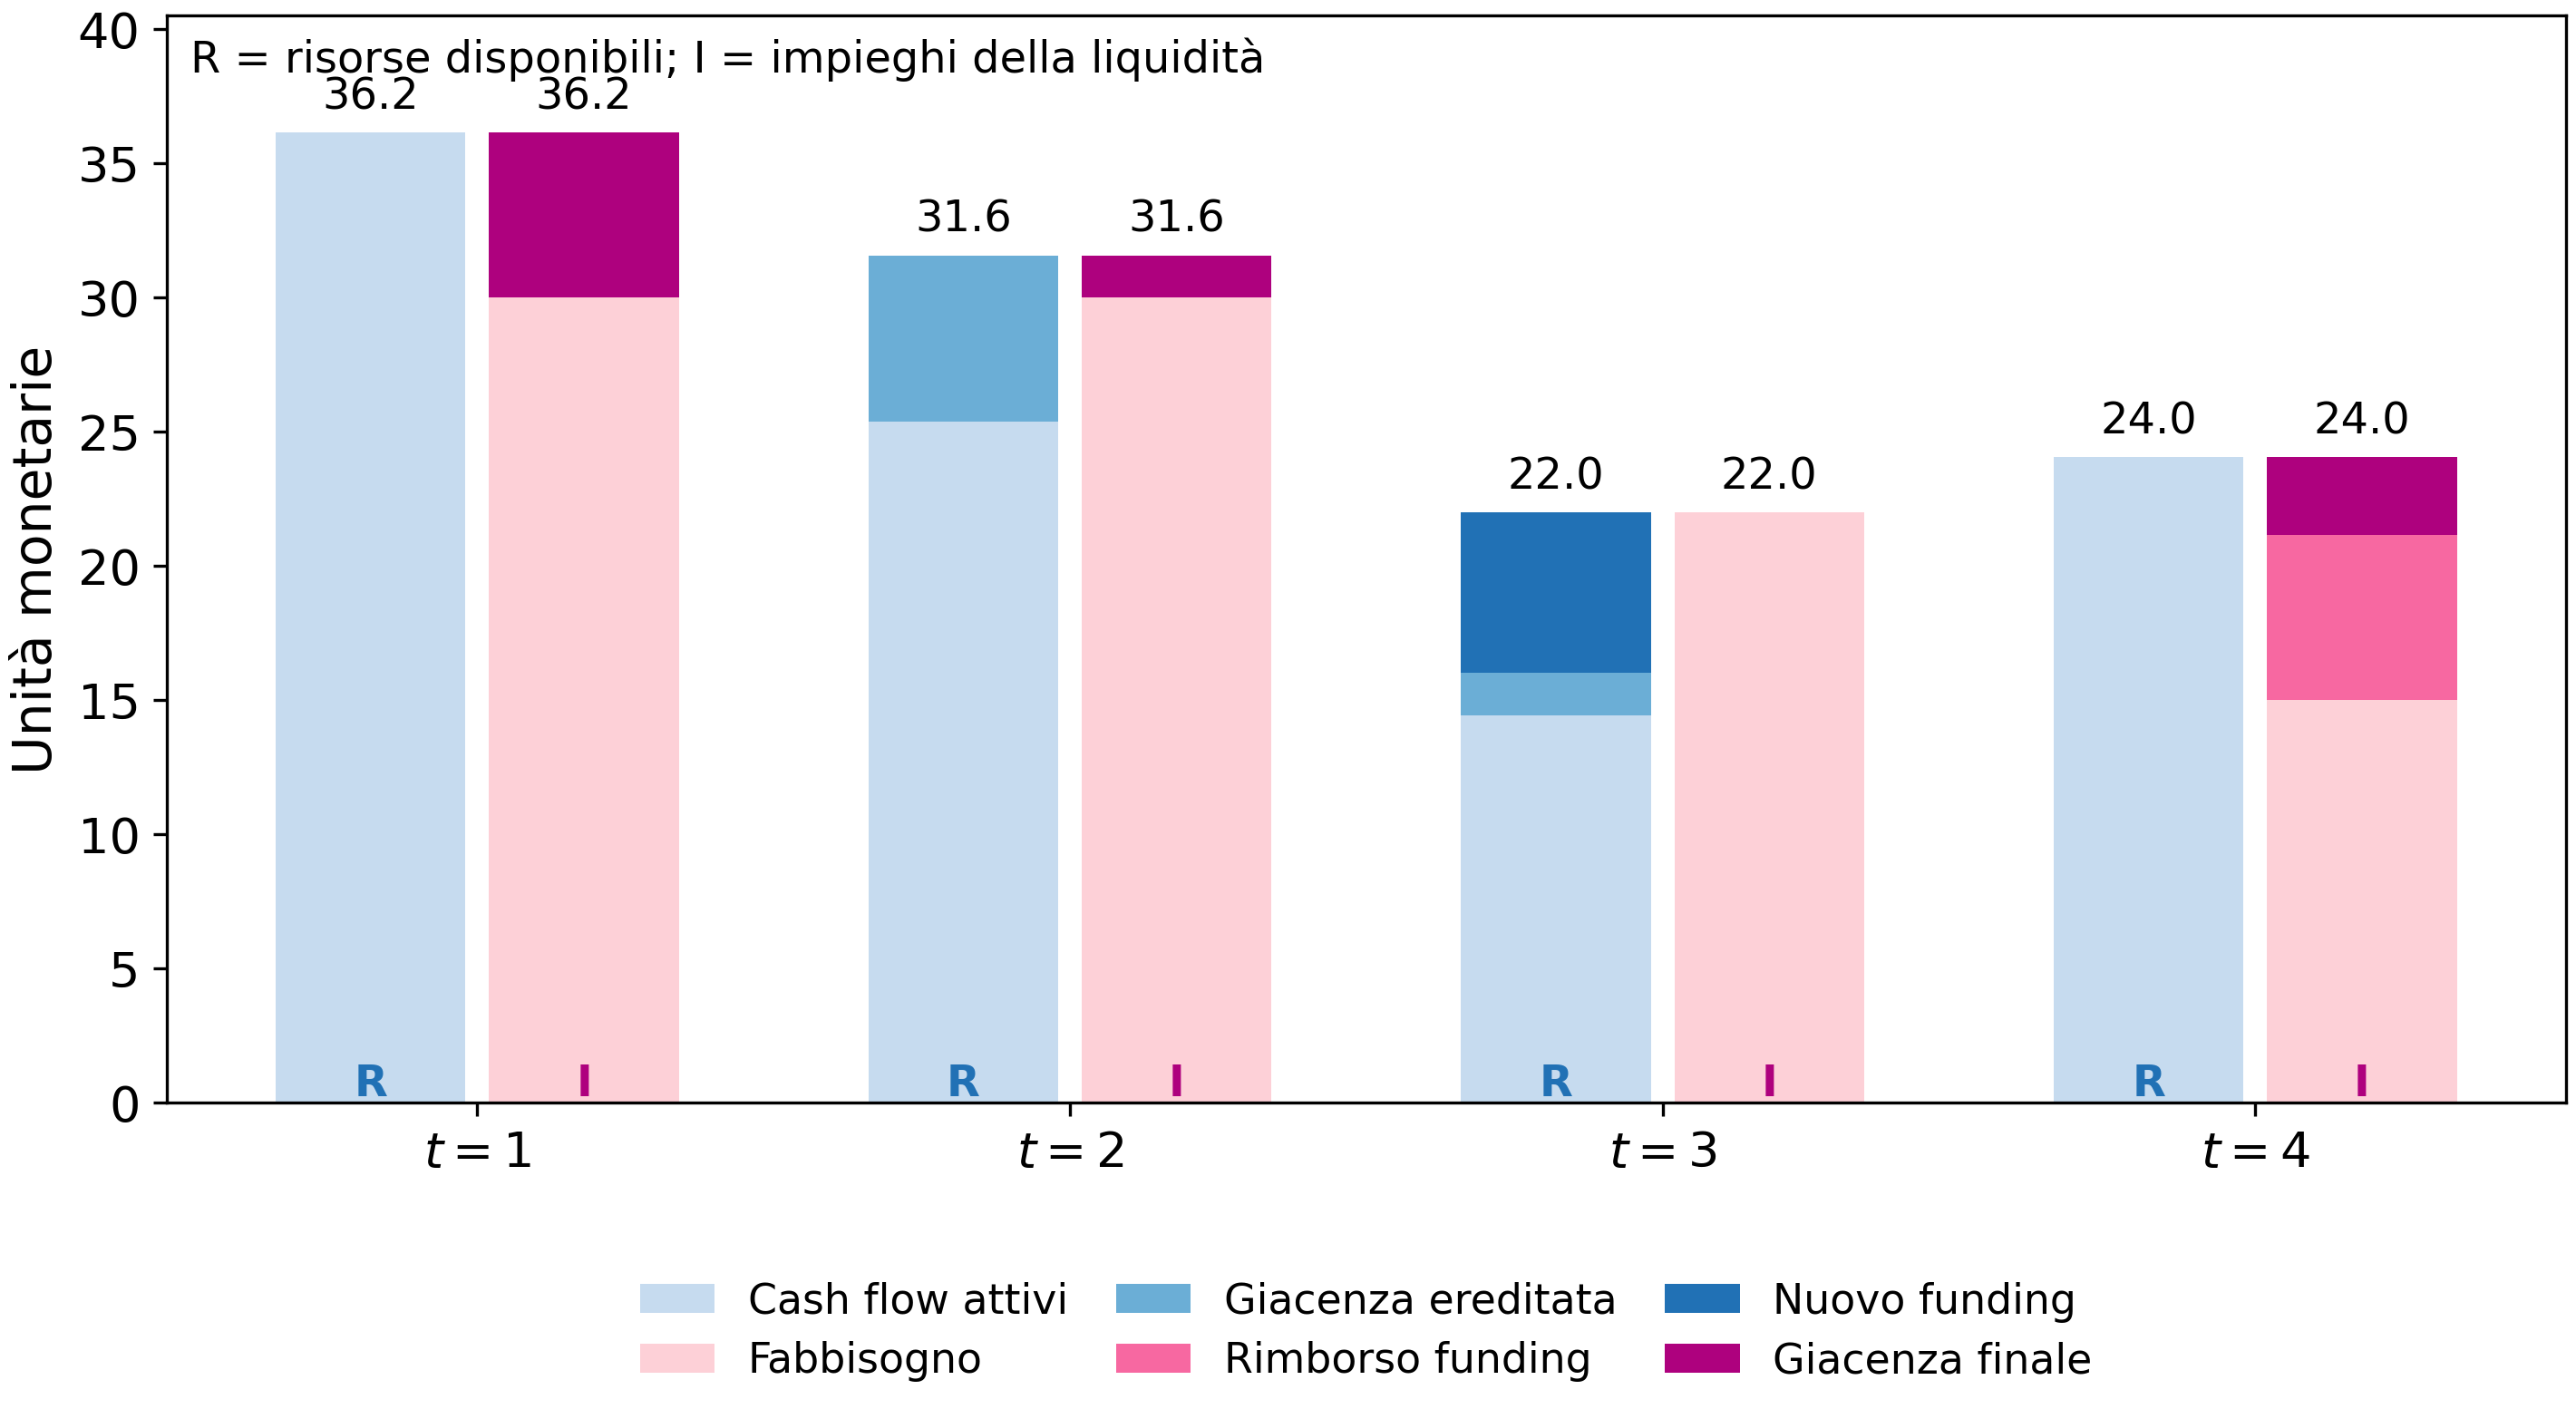
\includegraphics[width=0.94\textwidth]
{../graphics/Cap12_ALM_profili_ottimi.png}
\caption{Risorse e impieghi nelle quattro date della soluzione ottima del
caso SVB multiperiodale. La liquidit\`a accumulata trasferisce risorse verso
le date successive, mentre alla data $t=3$ il modello utilizza interamente
la capacit\`a di funding disponibile.}
\label{fig:cap12-alm-profili-ottimi}
\end{figure}

Infine, il contributo della composizione dell'attivo \`e

\[
c'x^*
\approx
3.7020,
\]

gli interessi sulle giacenze sono

\[
\sum_{t=1}^{3}r_tg_t^*
\approx
0.0402,
\]

e il costo del funding \`e

\[
\sum_{t=1}^{3}\rho_tu_t^*
=
0.1500.
\]

Pertanto,

\[
\Pi^*
\approx
3.5922.
\]

Il confronto diretto tra questo valore e il valore ottimo del problema
statico,

\[
z^{\mathrm{stat}}
\approx
3.765,
\]

non sarebbe tuttavia del tutto corretto, poich\'e la funzione obiettivo ALM
contiene anche interessi sulle giacenze e costi di funding. Per isolare
l'effetto sulla sola composizione dell'attivo \`e pi\`u informativo confrontare

\[
c'x^{\mathrm{stat}}
\approx
3.765
\]

con

\[
c'x^*
\approx
3.702.
\]

I vincoli prudenziali non risultano determinanti nella nuova soluzione:

\[
\ell'x^*
\approx
4.885
<
7,
\qquad
x_3^*=0<30.
\]

Al contrario, il limite

\[
u_3\leq6
\]

\`e raggiunto.

La sola osservazione dei vincoli attivi indica dove si concentra la scarsit\`a,
ma non ne misura ancora il valore economico. La domanda naturale diventa
quindi quale sia il valore marginale di una unit\`a aggiuntiva di risorse
disponibili nelle diverse date. Questo problema conduce direttamente
all'interpretazione duale dei bilanci temporali.

\section{Dualit\`a nell'ALM: il valore della liquidit\`a nelle diverse date}

\label{sec:cap12-dualita-alm}

Il Capitolo~\ref{cap:programmazione-lineare} ha mostrato che una variabile
duale consente di attribuire un valore marginale a una risorsa o a un
requisito del problema primale. Nel modello statico, un unico prezzo ombra
era associato al requisito aggregato di liquidit\`a.

Nel modello ALM la liquidit\`a non \`e invece concentrata in un solo vincolo.
Esiste un bilancio monetario per ciascuna data:

\[
a_t'x
+
(1+r_{t-1})g_{t-1}
+
u_t
-
(1+\rho_{t-1})u_{t-1}
-
g_t
=
d_t,
\]

con le opportune modifiche alla prima e all'ultima data.

La dualit\`a permette quindi di passare da un unico valore della liquidit\`a
a un profilo temporale di valori marginali.

\subsection{Il valore marginale dei bilanci temporali}

Associamo al bilancio della data $t$ una variabile duale

\[
\lambda_t\in\mathbb{R}.
\]

Poich\'e il vincolo di bilancio \`e un'uguaglianza, $\lambda_t$ non \`e
soggetta a un vincolo di segno.

Scrivendo il bilancio nella forma

\[
\text{risorse nette alla data }t=d_t,
\]

la convenzione adottata implica

\[
\frac{\partial\Pi^*}{\partial d_t}
=
-\lambda_t^*.
\]

Per una piccola variazione $\Delta d_t$ si ha quindi

\[
\Delta\Pi^*
\approx
-\lambda_t^*\,\Delta d_t.
\]

Se

\[
\lambda_t^*>0,
\]

un aumento unitario del fabbisogno alla data $t$ riduce localmente il
risultato ottimo di $\lambda_t^*$.

Equivalentemente, $\lambda_t^*$ misura il valore marginale di una unit\`a
aggiuntiva di liquidit\`a disponibile in quella stessa data.

Il passaggio rispetto al modello statico \`e quindi

\[
\boxed{
\text{un prezzo della liquidit\`a}
\quad\longrightarrow\quad
\text{un prezzo della liquidit\`a per ciascuna data}.
}
\]

\subsection{I valori duali nel caso SVB multiperiodale}

Per la soluzione della Sezione~\ref{sec:cap12-caso-svb-multiperiodale}, i
valori marginali dei quattro bilanci sono

\[
\lambda^*
\approx
\begin{pmatrix}
0.04524\\
0.04004\\
0.03383\\
0
\end{pmatrix}.
\]

La relazione tra posizione primale e valore marginale pu\`o essere riassunta
come segue:

\[
\begin{array}{c|c|c|c}
\hline
t & g_t^* & u_t^* & \lambda_t^*\\
\hline
1 & 6.152 & 0 & 0.04524\\
2 & 1.567 & 0 & 0.04004\\
3 & 0     & 6 & 0.03383\\
4 & 2.890 & - & 0\\
\hline
\end{array}
\]

Alla prima data, per esempio,

\[
\lambda_1^*
\approx
0.04524
\]

significa che un aumento marginale di una unit\`a del fabbisogno $d_1$
riduce il risultato ottimo di circa

\[
0.04524.
\]

Alla seconda e alla terza data il costo marginale rimane positivo, ma
diminuisce rispettivamente a

\[
0.04004
\]

e

\[
0.03383.
\]

Il risultato alla data finale richiede invece un'interpretazione specifica.

Poich\'e

\[
g_4^*
\approx
2.890>0
\]

e la giacenza terminale non riceve un valore nella funzione obiettivo, un
piccolo aumento di $d_4$ pu\`o essere assorbito semplicemente riducendo
$g_4$.

Localmente,

\[
\lambda_4^*=0.
\]

Questo non significa che la liquidit\`a alla data finale non abbia valore in
generale. Il risultato dipende dalla specificazione terminale del modello e
rimane valido finch\'e il margine rappresentato da $g_4^*$ non viene
esaurito.

\begin{figure}[htbp]
\centering
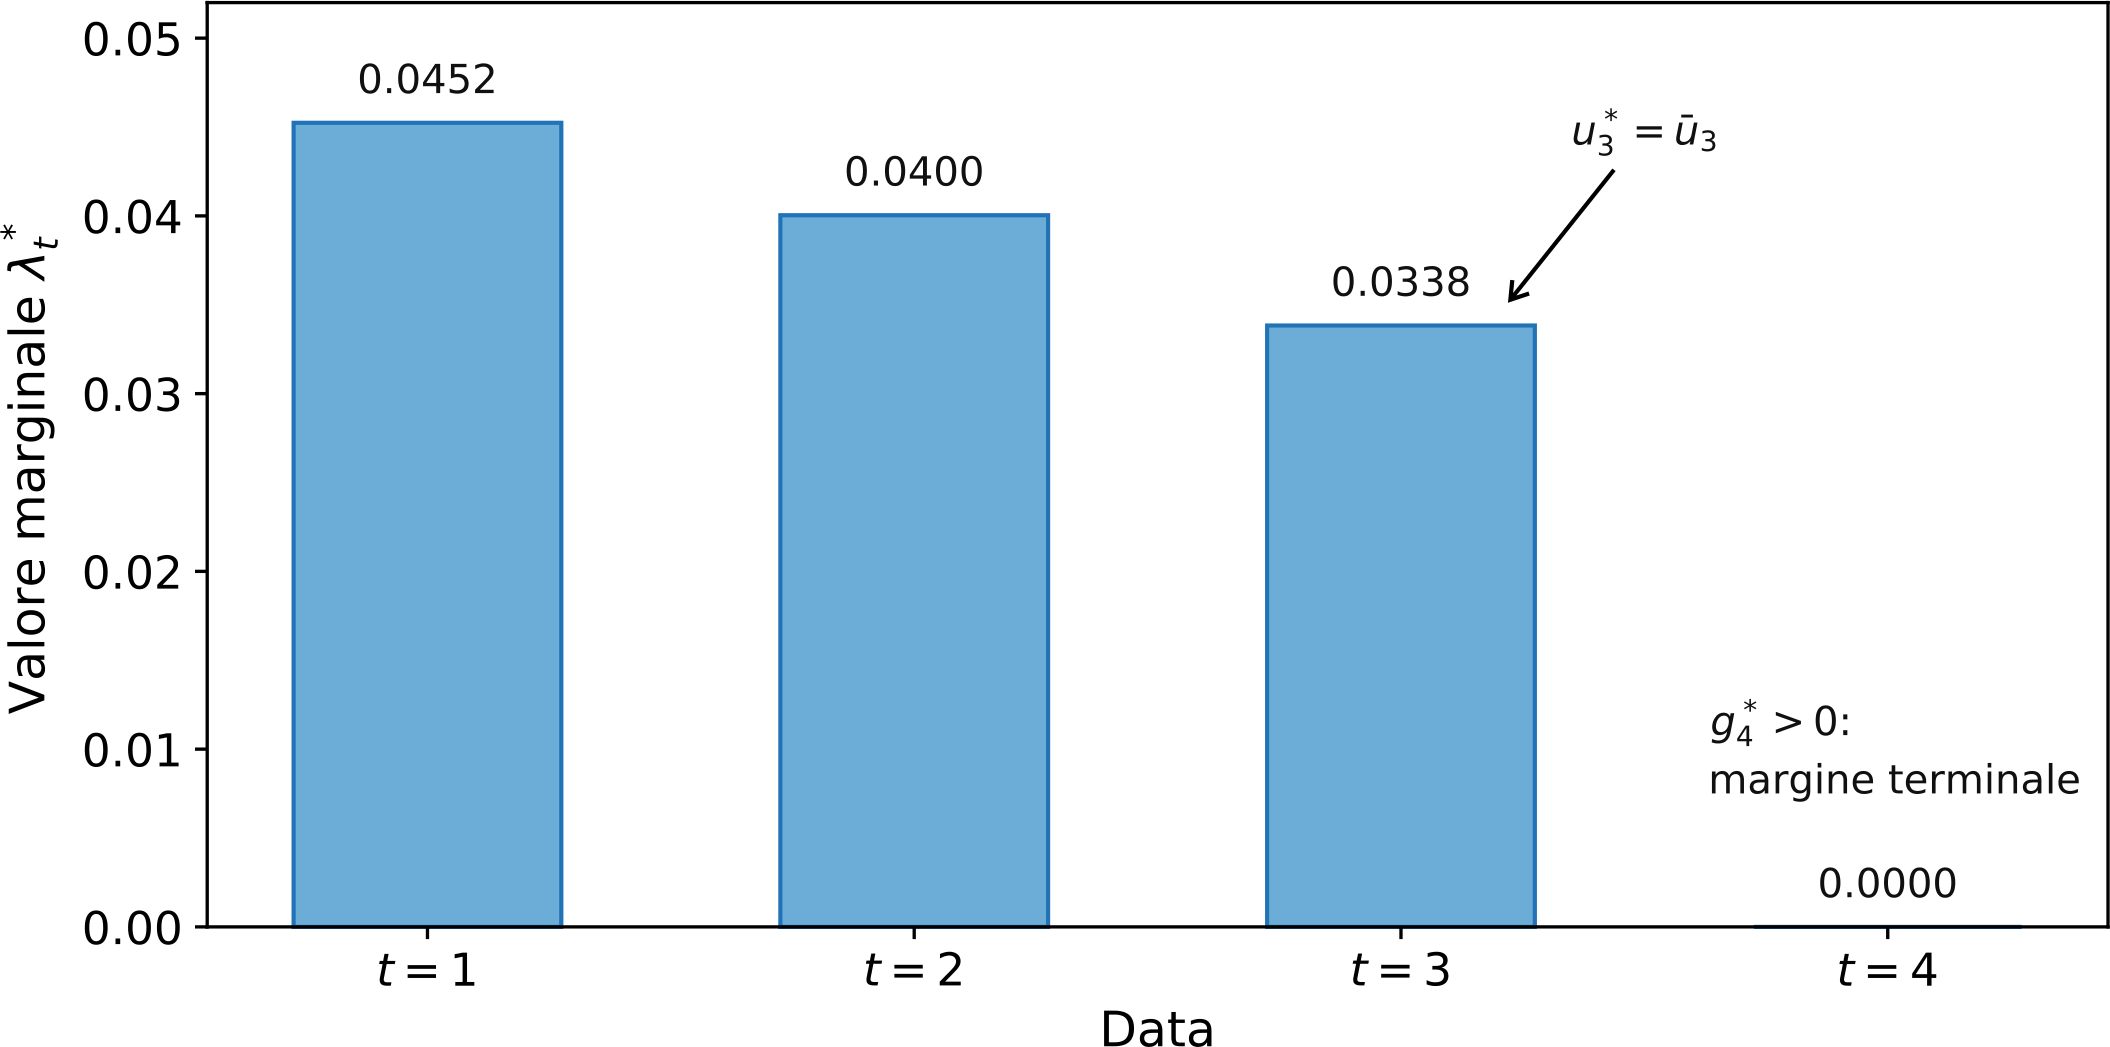
\includegraphics[width=0.88\textwidth]
{../graphics/Cap12_prezzi_ombra_scadenze.png}
\caption{Valore marginale della liquidit\`a nelle quattro date del caso SVB
multiperiodale. Il valore terminale \`e nullo localmente perch\'e la
soluzione presenta una giacenza finale positiva; alla data $t=3$ la banca
utilizza invece interamente la capacit\`a di funding disponibile.}
\label{fig:cap12-prezzi-ombra-scadenze}
\end{figure}

La Figura~\ref{fig:cap12-prezzi-ombra-scadenze} mostra un profilo decrescente
dei valori marginali. Tale andamento appartiene alla soluzione considerata e
non costituisce una propriet\`a generale dei modelli ALM: dipende dai cash
flow, dai fabbisogni, dai tassi, dai limiti di funding e dalla condizione
terminale.

\subsection{Il valore della capacit\`a di funding}

Un secondo valore duale rilevante riguarda il limite

\[
u_t\leq\bar u_t.
\]

Indichiamo con

\[
\lambda_{u,t}^*
\]

il valore marginale associato alla capacit\`a massima di funding. Localmente,

\[
\Delta\Pi^*
\approx
\lambda_{u,t}^*\,\Delta\bar u_t.
\]

Nella soluzione considerata,

\[
u_1^*<\bar u_1,
\qquad
u_2^*<\bar u_2,
\]

e i corrispondenti valori marginali sono nulli.

Alla terza data vale invece

\[
u_3^*
=
\bar u_3
=
6,
\]

e il valore duale associato al limite risulta

\[
\lambda_{u,3}^*
\approx
0.00883.
\]

Una piccola espansione della capacit\`a di funding disponibile alla data $3$
aumenterebbe quindi il valore ottimo di circa $0.00883$ per ogni unit\`a
aggiuntiva di capacit\`a.

Il risultato completa l'informazione fornita dalla soluzione primale:
l'uguaglianza

\[
u_3^*=\bar u_3
\]

individua una risorsa completamente utilizzata, mentre il corrispondente
valore duale misura quanto sarebbe economicamente utile, localmente,
allentarne il limite.

\section{Limiti del modello e passaggio all'incertezza}

\label{sec:cap12-limiti-incertezza}

Il modello sviluppato nelle sezioni precedenti permette di coordinare
composizione dell'attivo, liquidit\`a e funding lungo pi\`u date. La sua
struttura temporale \`e quindi pi\`u ricca di quella del problema statico del
Capitolo 11.

Rimane tuttavia un'ipotesi particolarmente forte: al tempo $0$ la banca
conosce l'intera traiettoria dei coefficienti che determineranno il problema
nelle date future.

\subsection{Che cosa significa deterministico}

Nel modello del capitolo sono noti al tempo $0$, tra gli altri,

\[
A^{\mathrm{CF}},
\qquad
d_t,
\qquad
r_t,
\qquad
\rho_t,
\qquad
\bar u_t.
\]

L'ipotesi deterministica non richiede che tali coefficienti siano costanti
nel tempo. Nel caso SVB multiperiodale, per esempio,

\[
r_1\neq r_2\neq r_3
\]

e anche la capacit\`a di funding varia:

\[
\bar u_1>\bar u_2>\bar u_3.
\]

Ci\`o che caratterizza il modello come deterministico \`e invece il fatto che
l'intero percorso

\[
\left\{
A^{\mathrm{CF}},
d_t,
r_t,
\rho_t,
\bar u_t
\right\}_{t=1}^{T}
\]

sia considerato noto quando il problema viene risolto.

Di conseguenza, la banca pu\`o determinare fin dal tempo $0$ l'intero piano

\[
x^*,
\qquad
g_1^*,\ldots,g_T^*,
\qquad
u_1^*,\ldots,u_{T-1}^*.
\]

Il modello risponde quindi alla domanda:

\[
\boxed{
\begin{array}{c}
\text{quale sarebbe il piano ottimo se la traiettoria futura}\\
\text{dei coefficienti fosse conosciuta?}
\end{array}
}
\]

Questa rappresentazione costituisce un benchmark utile, ma non descrive
completamente il problema decisionale affrontato da una banca reale.

\subsection{Quali elementi possono diventare incerti}

Nella realt\`a, alla data iniziale la banca non conosce con certezza le
condizioni che si manifesteranno nelle date successive.

Il vettore deterministico introdotto nella
Sezione~\ref{sec:cap12-ambiente-deterministico},

\[
\bar Z_t
=
(\bar R_t,\bar C_t,\bar F_t),
\]

pu\`o essere sostituito, in una rappresentazione incerta, da uno stato
economico-finanziario

\[
Z_t
=
(R_t,C_t,F_t).
\]

La distinzione \`e sostanziale. Nel primo caso

\[
\bar Z_t
\]

\`e un valore noto al momento della formulazione; nel secondo

\[
Z_t
\]

rappresenta uno stato futuro che non \`e ancora conosciuto al tempo $0$.

L'incertezza pu\`o quindi propagarsi ai coefficienti dell'ALM. In forma
schematica,

\[
Z_t
\quad\longrightarrow\quad
r_t,\ \rho_t,\ \bar u_t,
\]

e, quando economicamente appropriato, anche ai cash flow disponibili e ai
fabbisogni.

In particolare, il fabbisogno deterministico

\[
d_t
\]

pu\`o essere sostituito da una quantit\`a futura

\[
D_t,
\]

il cui valore dipende dalle condizioni che si realizzano.

La struttura concettuale discussa nella
Sezione~\ref{sec:cap12-stato-banca} suggerisce pi\`u precisamente

\[
D_t
=
d(Z_t,h_t),
\]

dove

\[
h_t
=
h(X_t,Z_t)
\]

dipende sia dall'ambiente esterno sia dallo stato della banca.

Non renderemo qui operative queste relazioni. Esse servono a individuare il
punto nel quale l'ipotesi deterministica dovr\`a essere abbandonata.

\subsection{Dal piano unico alle decisioni contingenti}

L'effetto pi\`u importante dell'incertezza riguarda la natura stessa delle
decisioni.

Nel modello deterministico il valore futuro di

\[
u_t
\]

pu\`o essere scelto gi\`a al tempo $0$, perch\'e i fabbisogni, i costi e la
capacit\`a di funding futuri sono noti.

In presenza di incertezza questa impostazione non \`e generalmente
appropriata. Il funding da utilizzare alla data $t$ dovrebbe poter dipendere
dalle condizioni effettivamente osservate a quella data.

Si passa quindi concettualmente da

\[
u_t
=
\text{numero fissato al tempo }0
\]

a una decisione del tipo

\[
u_t
=
u_t(\text{informazione disponibile alla data }t).
\]

La composizione iniziale $x$, invece, deve essere scelta prima di conoscere
gli stati futuri. Essa deve quindi tenere conto delle conseguenze che potranno
emergere lungo pi\`u evoluzioni possibili.

Il passaggio fondamentale pu\`o essere sintetizzato come

\[
\boxed{
\begin{array}{ccc}
\text{ALM deterministico}
&
\longrightarrow
&
\text{ALM sotto incertezza}
\\[4pt]
\text{una traiettoria nota}
&&
\text{pi\`u evoluzioni possibili}
\\[4pt]
\text{un piano fissato al tempo }0
&&
\text{decisioni compatibili con l'informazione disponibile}.
\end{array}
}
\]

Anche i valori duali ottenuti nelle sezioni precedenti devono essere letti
alla luce di questa distinzione. Essi misurano valori marginali
\emph{condizionati alla traiettoria deterministica assunta}: non incorporano
da soli il rischio che tassi, fabbisogni o disponibilit\`a di funding seguano
percorsi differenti.

Il modello deterministico rimane quindi un riferimento essenziale. Permette
di isolare la struttura dei bilanci intertemporali, identificare le date nelle
quali le risorse risultano scarse e attribuire loro un valore marginale.

Il passo successivo consiste nel mantenere questa struttura temporale
abbandonando l'ipotesi di conoscenza perfetta del futuro.

\section{Esercizi svolti}

\label{sec:cap12-esercizi-svolti}

Gli esercizi seguenti consolidano tre passaggi centrali del capitolo:
la formulazione di un problema ALM, la verifica della fattibilit\`a
intertemporale e l'interpretazione dei valori duali.

\begin{exercise}[Dalla descrizione del problema alla formulazione]

\label{ex:cap12-formulazione-alm-solver}

Una banca dispone al tempo $0$ di $50$ unit\`a monetarie, che devono essere
interamente allocate tra tre classi di attivo.

La prima classe rappresenta cassa e riserve. Produce un contributo economico
pari all'1\% dell'investimento e l'intero ammontare investito diventa
disponibile come liquidit\`a alla data $1$.

La seconda classe \`e costituita da titoli a breve scadenza. Produce un
contributo economico del $2.5\%$; il $60\%$ dell'investimento iniziale diventa
disponibile alla data $1$ e il restante $40\%$ alla data $2$.

La terza classe \`e costituita da prestiti. Produce un contributo economico
del $4.5\%$; il $10\%$ dell'investimento iniziale diventa disponibile alla
data $1$, il $30\%$ alla data $2$ e il restante $60\%$ alla data $3$.

I fabbisogni di liquidit\`a alle tre date sono rispettivamente

\[
25,\qquad18,\qquad12.
\]

La liquidit\`a non utilizzata alla data $1$ pu\`o essere trasferita alla data
$2$ con un rendimento dello $0.5\%$; quella non utilizzata alla data $2$ pu\`o
essere trasferita alla data $3$ con un rendimento dello $0.6\%$.

La banca pu\`o inoltre raccogliere funding alla data $1$ fino a un massimo di
$4$ unit\`a, con costo dell'1.5\%, e alla data $2$ fino a un massimo di $3$
unit\`a, con costo del $2\%$. Il funding raccolto in una data deve essere
rimborsato alla data successiva.

In uno scenario di stress, le perdite unitarie associate alle tre classi di
attivo sono rispettivamente

\[
0,\qquad0.03,\qquad0.08,
\]

e la perdita complessiva non pu\`o superare $2.6$.

Infine, l'investimento nei prestiti non pu\`o superare $25$ unit\`a.

A partire esclusivamente da queste informazioni:

\begin{enumerate}

\item individuare le variabili decisionali;

\item costruire i vettori e la matrice dei parametri necessari;

\item formulare matematicamente la funzione obiettivo;

\item scrivere il vincolo sulle risorse iniziali, i tre bilanci di liquidit\`a,
i vincoli prudenziali, i limiti sul funding e le condizioni di non negativit\`a;

\item raccogliere tutte le variabili in un unico vettore $z$ e scrivere il
problema nella forma matriciale necessaria per l'utilizzo di un solver LP:

\[
\min\;\widetilde c'z,
\qquad
A_{\mathrm{ub}}z\leq b_{\mathrm{ub}},
\qquad
A_{\mathrm{eq}}z=b_{\mathrm{eq}},
\]

specificando inoltre i bounds delle variabili.
\end{enumerate}

\end{exercise}

\noindent
\textbf{Soluzione.}

\begin{enumerate}

\item \textbf{Variabili decisionali.}

Indichiamo con

\[
x_1,\qquad x_2,\qquad x_3
\]

gli importi investiti al tempo $0$ rispettivamente in cassa e riserve,
titoli a breve scadenza e prestiti.

Le giacenze di liquidit\`a residue alle tre date sono

\[
g_1,\qquad g_2,\qquad g_3,
\]

mentre il funding raccolto alle prime due date \`e rappresentato da

\[
u_1,\qquad u_2.
\]

Non viene introdotto nuovo funding alla data finale, poich\'e il relativo
rimborso cadrebbe oltre l'orizzonte del modello.

Tutte le variabili sono non negative:

\[
x_j\geq0,
\qquad
j=1,2,3,
\]

\[
g_t\geq0,
\qquad
t=1,2,3,
\]

\[
u_t\geq0,
\qquad
t=1,2.
\]


\item \textbf{Costruzione dei parametri.}

Dalla descrizione delle tre classi di attivo si ricava il vettore dei
contributi economici unitari

\[
c
=
\begin{pmatrix}
0.010\\
0.025\\
0.045
\end{pmatrix}.
\]

I profili temporali con cui le risorse investite nelle tre classi diventano
disponibili determinano la matrice dei cash flow

\[
A^{\mathrm{CF}}
=
\begin{pmatrix}
1.00 & 0.60 & 0.10\\
0    & 0.40 & 0.30\\
0    & 0    & 0.60
\end{pmatrix}.
\]

Il vettore dei fabbisogni \`e

\[
d
=
\begin{pmatrix}
25\\
18\\
12
\end{pmatrix}.
\]

I rendimenti delle giacenze sono

\[
r_1=0.005,
\qquad
r_2=0.006,
\]

mentre i costi del funding sono

\[
\rho_1=0.015,
\qquad
\rho_2=0.020.
\]

La capacit\`a massima di funding \`e

\[
\bar u_1=4,
\qquad
\bar u_2=3.
\]

Il vettore delle perdite unitarie nello scenario di stress \`e

\[
\ell
=
\begin{pmatrix}
0\\
0.03\\
0.08
\end{pmatrix},
\]

con limite complessivo

\[
K=2.6.
\]

Infine, il limite di concentrazione sui prestiti \`e

\[
x_3\leq25.
\]


\item \textbf{Funzione obiettivo.}

In forma simbolica, per un orizzonte con $T=3$ date future, la funzione
obiettivo \`e

\[
\max\;
\Pi(x,g,u)
=
c'x
+
\sum_{t=1}^{2}r_tg_t
-
\sum_{t=1}^{2}\rho_tu_t.
\]

Sostituendo i valori numerici si ottiene

\[
\boxed{
\max\;
0.010x_1
+
0.025x_2
+
0.045x_3
+
0.005g_1
+
0.006g_2
-
0.015u_1
-
0.020u_2.
}
\]


\item \textbf{Vincoli del modello ALM.}

Le risorse iniziali devono essere interamente allocate:

\[
x_1+x_2+x_3=50.
\]

Alla prima data sono disponibili i cash flow prodotti dagli attivi e il
funding eventualmente raccolto in $t=1$. Il bilancio di liquidit\`a \`e

\[
x_1
+
0.60x_2
+
0.10x_3
+
u_1
=
25+g_1,
\]

ovvero

\[
x_1
+
0.60x_2
+
0.10x_3
+
u_1
-
g_1
=
25.
\]

Alla seconda data diventano disponibili i nuovi cash flow degli attivi, la
giacenza precedente capitalizzata e il nuovo funding. Deve inoltre essere
rimborsato il funding raccolto alla prima data:

\[
0.40x_2
+
0.30x_3
+
1.005g_1
+
u_2
=
18
+
1.015u_1
+
g_2.
\]

Pertanto,

\[
0.40x_2
+
0.30x_3
+
1.005g_1
+
u_2
-
1.015u_1
-
g_2
=
18.
\]

Alla data finale non viene raccolto nuovo funding:

\[
0.60x_3
+
1.006g_2
=
12
+
1.020u_2
+
g_3,
\]

ossia

\[
0.60x_3
+
1.006g_2
-
1.020u_2
-
g_3
=
12.
\]

Il vincolo sulla perdita nello scenario di stress \`e

\[
0.03x_2+0.08x_3\leq2.6.
\]

Il limite di concentrazione sui prestiti \`e

\[
x_3\leq25.
\]

I limiti sul funding sono

\[
0\leq u_1\leq4,
\qquad
0\leq u_2\leq3.
\]

Infine,

\[
x_1,x_2,x_3\geq0,
\qquad
g_1,g_2,g_3\geq0.
\]

Il programma lineare completo \`e quindi

\[
\begin{array}{ll}

\max
&
\displaystyle
0.010x_1
+
0.025x_2
+
0.045x_3
\\
& +
0.005g_1
+
0.006g_2
-
0.015u_1
-
0.020u_2
\\[8pt]

\mbox{soggetto a}
&
x_1+x_2+x_3=50,
\\[6pt]

&
x_1+0.60x_2+0.10x_3+u_1-g_1=25,
\\[6pt]

&
0.40x_2+0.30x_3+1.005g_1
+u_2-1.015u_1-g_2=18,
\\[6pt]

&
0.60x_3+1.006g_2-1.020u_2-g_3=12,
\\[6pt]

&
0.03x_2+0.08x_3\leq2.6,
\\[6pt]

&
x_3\leq25,
\\[6pt]

&
0\leq u_1\leq4,
\qquad
0\leq u_2\leq3,
\\[6pt]

&
x_1,x_2,x_3,g_1,g_2,g_3\geq0.
\end{array}
\]


\item \textbf{Forma matriciale per il solver.}

Raccogliamo le variabili secondo l'ordine

\[
z
=
\begin{pmatrix}
x_1&
x_2&
x_3&
g_1&
g_2&
g_3&
u_1&
u_2
\end{pmatrix}'.
\]

Rispetto a questo ordinamento, il vettore dei coefficienti della funzione
obiettivo in massimizzazione \`e

\[
c^{\mathrm{ALM}}
=
\begin{pmatrix}
0.010\\
0.025\\
0.045\\
0.005\\
0.006\\
0\\
-0.015\\
-0.020
\end{pmatrix}.
\]

Poich\'e il solver \texttt{scipy.optimize.linprog} utilizza una formulazione
in minimizzazione, si pone

\[
\widetilde c
=
-c^{\mathrm{ALM}},
\]

e quindi

\[
\widetilde c
=
\begin{pmatrix}
-0.010\\
-0.025\\
-0.045\\
-0.005\\
-0.006\\
0\\
0.015\\
0.020
\end{pmatrix}.
\]

Il problema passato al solver ha pertanto funzione obiettivo

\[
\min\;\widetilde c'z.
\]

Il vincolo sulle risorse iniziali e i tre bilanci temporali sono uguaglianze.
Essi possono essere raccolti nella matrice

\[
A_{\mathrm{eq}}
=
\begin{pmatrix}
1 & 1    & 1    & 0     & 0     & 0  & 0      & 0\\
1 & 0.60 & 0.10 & -1    & 0     & 0  & 1      & 0\\
0 & 0.40 & 0.30 & 1.005 & -1    & 0  & -1.015 & 1\\
0 & 0    & 0.60 & 0     & 1.006 & -1 & 0      & -1.020
\end{pmatrix},
\]

con

\[
b_{\mathrm{eq}}
=
\begin{pmatrix}
50\\
25\\
18\\
12
\end{pmatrix}.
\]

I due vincoli espressi come disuguaglianze sono

\[
0.03x_2+0.08x_3\leq2.6
\]

e

\[
x_3\leq25.
\]

Pertanto,

\[
A_{\mathrm{ub}}
=
\begin{pmatrix}
0 & 0.03 & 0.08 & 0 & 0 & 0 & 0 & 0\\
0 & 0    & 1    & 0 & 0 & 0 & 0 & 0
\end{pmatrix},
\]

e

\[
b_{\mathrm{ub}}
=
\begin{pmatrix}
2.6\\
25
\end{pmatrix}.
\]

Infine, i limiti delle variabili sono

\[
\begin{array}{c|c}
\text{variabili} & \text{bounds}\\
\hline
x_1,x_2,x_3 & [0,+\infty)\\
g_1,g_2,g_3 & [0,+\infty)\\
u_1 & [0,4]\\
u_2 & [0,3].
\end{array}
\]

La formulazione da trasmettere al solver \`e quindi completamente
specificata da

\[
\boxed{
\begin{array}{c}
\displaystyle
\min\;\widetilde c'z
\\[6pt]
A_{\mathrm{eq}}z=b_{\mathrm{eq}},
\\[4pt]
A_{\mathrm{ub}}z\leq b_{\mathrm{ub}},
\\[4pt]
\underline z\leq z\leq\overline z.
\end{array}
}
\]

Il passaggio decisivo non consiste nell'applicazione del solver, ma nella
traduzione coerente della descrizione finanziaria in variabili, coefficienti
e vincoli. Una volta costruita correttamente questa rappresentazione, il
problema \`e un programma lineare standard e pu\`o essere risolto
numericamente senza ulteriori modifiche alla sua struttura economica.

\end{enumerate}


\begin{exercise}[Fattibilit\`a temporale e limite al funding]

\label{ex:cap12-fattibilita-funding}

Una banca ha investito al tempo $0$ in due classi di attivo secondo la
composizione

\[
x=
\begin{pmatrix}
20\\
20
\end{pmatrix}.
\]

La distribuzione temporale dei cash flow prodotti dagli attivi \`e descritta
dalla matrice

\[
A^{\mathrm{CF}}
=
\begin{pmatrix}
0.70 & 0.10\\
0.30 & 0.30\\
0    & 0.60
\end{pmatrix}.
\]

I fabbisogni di liquidit\`a alle tre date sono

\[
d'
=
(15,\;14,\;8).
\]

La liquidit\`a residua alla prima data pu\`o essere trasferita alla seconda
con rendimento

\[
r_1=0.005.
\]

Si assume che non venga raccolto funding alla prima data,

\[
u_1=0,
\]

mentre alla seconda data la banca pu\`o ricorrere a funding che dovr\`a essere
rimborsato alla data finale con costo

\[
\rho_2=0.020.
\]

In condizioni ordinarie la capacit\`a di funding alla seconda data \`e

\[
\bar u_2=3.
\]

\begin{enumerate}

\item Calcolare il profilo temporale dei cash flow prodotto dagli attivi.

\item Verificare se la composizione assegnata permette di soddisfare i
fabbisogni alle tre date senza ricorrere al funding.

\item Determinare il funding minimo necessario alla seconda data e calcolare
la giacenza terminale risultante.

\item Supporre ora che la capacit\`a massima di funding alla seconda data si
riduca a

\[
\bar u_2=0.8.
\]

Stabilire se il piano rimane ammissibile e interpretare il risultato.

\end{enumerate}

\end{exercise}

\noindent
\textbf{Soluzione.}

\begin{enumerate}

\item Il profilo dei cash flow \`e

\[
A^{\mathrm{CF}}x
=
\begin{pmatrix}
0.70 & 0.10\\
0.30 & 0.30\\
0    & 0.60
\end{pmatrix}
\begin{pmatrix}
20\\
20
\end{pmatrix}
=
\begin{pmatrix}
16\\
12\\
12
\end{pmatrix}.
\]

\item Alla prima data, ponendo $u_1=0$,

\[
16=15+g_1,
\]

da cui

\[
g_1=1.
\]

Alla seconda data, in assenza di funding, le risorse disponibili sarebbero

\[
12+1.005(1)
=
13.005.
\]

Il fabbisogno \`e invece

\[
d_2=14.
\]

Pertanto

\[
13.005<14
\]

e la composizione non \`e temporalmente fattibile senza funding.

Il punto importante \`e che l'insufficienza emerge alla seconda data:
non pu\`o essere compensata utilizzando anticipatamente il cash flow pari a
$12$ che sar\`a disponibile soltanto alla data successiva.

\item Ponendo $g_2=0$, il bilancio della seconda data richiede

\[
12
+
1.005(1)
+
u_2
=
14.
\]

Il funding minimo \`e quindi

\[
u_2
=
14-13.005
=
0.995.
\]

Alla data finale il rimborso dovuto \`e

\[
1.020(0.995)
=
1.0149.
\]

Il bilancio terminale diventa

\[
12
=
8
+
1.0149
+
g_3,
\]

da cui

\[
g_3
=
2.9851.
\]

Il funding anticipa quindi $0.995$ unit\`a alla seconda data e genera alla
terza un rimborso pari a $1.0149$.

\item Se

\[
\bar u_2=0.8,
\]

il funding massimo disponibile sarebbe inferiore al fabbisogno minimo

\[
u_2^{\min}=0.995.
\]

La composizione considerata diventerebbe quindi non ammissibile:

\[
\bar u_2<u_2^{\min}.
\]

\end{enumerate}

L'esercizio distingue due concetti che non devono essere confusi:
l'esistenza di risorse lungo l'intero orizzonte e la loro disponibilit\`a
nella data nella quale devono essere utilizzate.


\begin{exercise}[Interpretazione dei valori duali]

\label{ex:cap12-valori-duali}

Nel caso SVB multiperiodale della
Sezione~\ref{sec:cap12-caso-svb-multiperiodale}, i valori marginali associati
ai quattro bilanci temporali sono

\[
\lambda^*
\approx
\begin{pmatrix}
0.04524\\
0.04004\\
0.03383\\
0
\end{pmatrix}.
\]

Il valore duale associato al limite

\[
u_3\leq\bar u_3
\]

\`e inoltre

\[
\lambda_{u,3}^*
\approx
0.00883.
\]

Si assuma che le variazioni considerate siano sufficientemente piccole da
non modificare la struttura della soluzione ottima.

\begin{enumerate}

\item Stimare l'effetto sul valore ottimo di un aumento

\[
\Delta d_2=0.5.
\]

\item Interpretare il risultato

\[
\lambda_4^*=0
\]

sapendo che

\[
g_4^*\approx2.890.
\]

\item Stimare l'effetto di un aumento unitario della capacit\`a di funding
alla terza data.

\item Spiegare perch\'e queste valutazioni devono essere interpretate
localmente.

\end{enumerate}

\end{exercise}

\noindent
\textbf{Soluzione.}

\begin{enumerate}

\item Per una piccola variazione del fabbisogno vale

\[
\Delta\Pi^*
\approx
-\lambda_2^*\,\Delta d_2.
\]

Pertanto

\[
\Delta\Pi^*
\approx
-0.04004(0.5)
=
-0.02002.
\]

Un aumento di mezzo punto del fabbisogno alla seconda data riduce quindi
localmente il valore ottimo di circa $0.020$.

\item Il risultato

\[
\lambda_4^*=0
\]

non significa che la liquidit\`a alla data finale sia priva di significato
finanziario.

Nella soluzione considerata esiste infatti una giacenza terminale positiva:

\[
g_4^*\approx2.890.
\]

Un piccolo aumento di $d_4$ pu\`o essere assorbito riducendo questa giacenza,
senza richiedere una modifica della composizione dell'attivo o del piano di
funding e senza modificare localmente la funzione obiettivo.

Il valore marginale nullo riflette quindi l'esistenza di un margine terminale
nella soluzione considerata.

\item Per il limite sulla capacit\`a di funding vale localmente

\[
\Delta\Pi^*
\approx
\lambda_{u,3}^*
\Delta\bar u_3.
\]

Con

\[
\Delta\bar u_3=1
\]

si ottiene

\[
\Delta\Pi^*
\approx
0.00883.
\]

Una unit\`a aggiuntiva di capacit\`a di funding alla terza data aumenterebbe
quindi il risultato massimo di circa $0.00883$.

\item I valori duali descrivono la pendenza locale della funzione valore
rispetto ai termini noti o ai limiti considerati.

Se una variazione sufficientemente ampia modifica i vincoli determinanti
della soluzione, anche i corrispondenti valori marginali possono cambiare.
Non \`e quindi corretto utilizzare indefinitamente lo stesso prezzo ombra
per variazioni arbitrarie dei parametri.

\end{enumerate}

Il confronto tra soluzione primale e valori duali mette in evidenza due
informazioni complementari: il primale mostra come vengono impiegate le
risorse disponibili, mentre il duale quantifica il valore marginale di una
variazione dei requisiti o delle risorse scarse.

\section{Esercizi proposti}

\label{sec:cap12-esercizi-proposti}


\begin{exercise}[Cash flow aggregati e distribuzione temporale]

\label{ex:cap12-proposto-cashflow-temporali}

Una banca considera tre classi di attivo. La matrice dei cash flow \`e

\[
A^{\mathrm{CF}}
=
\begin{pmatrix}
0.80 & 0.30 & 0.10\\
0.20 & 0.40 & 0.30\\
0    & 0.30 & 0.60
\end{pmatrix},
\]

e la composizione iniziale \`e

\[
x'
=
(10,\;20,\;30).
\]

I fabbisogni sono

\[
d'
=
(16,\;21,\;18).
\]

Si assumano, per semplicit\`a,

\[
r_1=r_2=0.
\]

Alla seconda data la banca pu\`o raccogliere funding al tasso

\[
\rho_2=0.02.
\]

\begin{enumerate}

\item Calcolare il profilo temporale

\[
A^{\mathrm{CF}}x.
\]

\item Verificare che il cash flow complessivo prodotto lungo l'orizzonte
coincida con l'ammontare inizialmente investito.

\item Stabilire se i fabbisogni possono essere soddisfatti senza funding,
tenendo conto del trasferimento delle giacenze tra date consecutive.

\item Determinare il funding minimo necessario alla seconda data e la
giacenza terminale risultante.

\item Spiegare perch\'e il confronto tra

\[
\sum_t d_t
\]

e il cash flow complessivo dell'attivo non \`e sufficiente per stabilire
l'ammissibilit\`a del piano.

\end{enumerate}

\end{exercise}

\noindent
\textit{Risultati:}

\[
A^{\mathrm{CF}}x
=
\begin{pmatrix}
17\\
19\\
24
\end{pmatrix},
\qquad
\sum_{t=1}^{3}(A^{\mathrm{CF}}x)_t=60.
\]

Alla prima data

\[
g_1=1.
\]

Alla seconda data rimane un deficit pari a $1$, per cui il funding minimo
\`e

\[
u_2=1.
\]

Tenendo conto del rimborso alla data finale,

\[
g_3=24-18-1.02=4.98.
\]


\begin{exercise}[Due portafogli con diversa struttura temporale]

\label{ex:cap12-proposto-confronto-portafogli}

Si consideri la matrice

\[
A^{\mathrm{CF}}
=
\begin{pmatrix}
0.90 & 0.40 & 0.10\\
0.10 & 0.40 & 0.30\\
0    & 0.20 & 0.60
\end{pmatrix}
\]

e i due portafogli

\[
x^{(A)}
=
\begin{pmatrix}
20\\
20\\
10
\end{pmatrix},
\qquad
x^{(B)}
=
\begin{pmatrix}
10\\
20\\
20
\end{pmatrix}.
\]

Entrambi utilizzano risorse iniziali pari a

\[
A_0=50.
\]

I fabbisogni sono

\[
d'
=
(22,\;16,\;10).
\]

I parametri finanziari sono

\[
r_1=0.004,
\qquad
r_2=0.005,
\]

\[
\rho_1=0.014,
\qquad
\rho_2=0.018,
\]

con

\[
\bar u_1=5,
\qquad
\bar u_2=4.
\]

\begin{enumerate}

\item Calcolare i profili

\[
A^{\mathrm{CF}}x^{(A)}
\qquad\text{e}\qquad
A^{\mathrm{CF}}x^{(B)}.
\]

\item Verificare se il portafoglio $A$ pu\`o soddisfare i tre fabbisogni
senza ricorrere al funding.

\item Per il portafoglio $B$, determinare il funding minimo necessario alla
prima data.

\item Verificare se la capacit\`a massima di funding alla seconda data
permette di proseguire il piano.

\item Interpretare la differenza tra i due portafogli dal punto di vista
dell'ALM.

\end{enumerate}

\end{exercise}

\noindent
\textit{Risultati:}

\[
A^{\mathrm{CF}}x^{(A)}
=
\begin{pmatrix}
27\\
13\\
10
\end{pmatrix},
\qquad
A^{\mathrm{CF}}x^{(B)}
=
\begin{pmatrix}
19\\
15\\
16
\end{pmatrix}.
\]

Il portafoglio $A$ \`e finanziariamente ammissibile senza funding.

Per il portafoglio $B$ occorre alla prima data

\[
u_1=3.
\]

Alla seconda data il funding minimo richiesto \`e circa

\[
u_2=4.042,
\]

ma

\[
\bar u_2=4.
\]

Il portafoglio $B$ non \`e quindi ammissibile.


\begin{exercise}[Formulazione completa di un problema ALM]

\label{ex:cap12-proposto-formulazione-completa}

Una banca dispone di

\[
A_0=50
\]

unit\`a monetarie e pu\`o scegliere tra tre classi di attivo.

I parametri dell'attivo sono

\[
\begin{array}{c|cc}
\hline
j & c_j & \ell_j\\
\hline
1 & 0.015 & 0\\
2 & 0.030 & 0.04\\
3 & 0.045 & 0.10\\
\hline
\end{array}
\]

e

\[
A^{\mathrm{CF}}
=
\begin{pmatrix}
0.90 & 0.40 & 0.10\\
0.10 & 0.40 & 0.30\\
0    & 0.20 & 0.60
\end{pmatrix}.
\]

I parametri temporali sono

\[
\begin{array}{c|cccc}
\hline
t & d_t & r_t & \rho_t & \bar u_t\\
\hline
1 & 20 & 0.004 & 0.014 & 5\\
2 & 18 & 0.005 & 0.018 & 4\\
3 & 10 & -     & -     & -\\
\hline
\end{array}
\]

e il limite alla perdita sotto stress \`e

\[
\ell'x\leq3.2.
\]

La terza classe di attivo non pu\`o inoltre superare

\[
x_3\leq20.
\]

\begin{enumerate}

\item Individuare tutte le variabili decisionali.

\item Scrivere la funzione obiettivo prima in forma simbolica e poi in forma
numerica.

\item Scrivere il vincolo sulle risorse iniziali.

\item Scrivere i tre bilanci di liquidit\`a prima in forma simbolica e poi
sostituendo i coefficienti numerici.

\item Completare il programma lineare con i limiti di funding, il vincolo di
stress, il limite di concentrazione e le condizioni di non negativit\`a.

\item Indicare quali coefficienti del modello potrebbero dipendere
dall'ambiente economico-finanziario

\[
\bar Z_t=(\bar R_t,\bar C_t,\bar F_t).
\]

\end{enumerate}

\end{exercise}

\noindent
\textit{Risultati di controllo:} le variabili sono

\[
x_1,x_2,x_3,
\qquad
g_1,g_2,g_3,
\qquad
u_1,u_2.
\]

La funzione obiettivo numerica \`e

\[
\max\;
0.015x_1+0.030x_2+0.045x_3
+0.004g_1+0.005g_2
-0.014u_1-0.018u_2.
\]

Il primo bilancio \`e

\[
0.90x_1+0.40x_2+0.10x_3+u_1-g_1=20.
\]


\begin{exercise}[Sensitivit\`a dei fabbisogni e della capacit\`a di funding]

\label{ex:cap12-proposto-sensitivita}

Nel caso SVB multiperiodale sono stati ottenuti i valori marginali

\[
\lambda^*
\approx
\begin{pmatrix}
0.04524\\
0.04004\\
0.03383\\
0
\end{pmatrix}
\]

per i quattro bilanci temporali.

Il valore duale del limite sulla capacit\`a di funding alla terza data \`e

\[
\lambda_{u,3}^*
\approx
0.00883.
\]

Si considerino variazioni sufficientemente piccole da non modificare la
struttura della soluzione ottima.

\begin{enumerate}

\item Stimare la variazione del valore ottimo se

\[
d_1
\]

aumenta di $0.4$.

\item Ripetere il calcolo per un aumento di $0.4$ di $d_3$.

\item Stimare il beneficio di un aumento pari a $0.5$ della capacit\`a

\[
\bar u_3.
\]

\item Spiegare perch\'e un piccolo aumento di $d_4$ ha valore marginale nullo
nella soluzione considerata.

\item Stabilire se sarebbe corretto utilizzare

\[
\lambda_4^*=0
\]

per valutare un aumento di $d_4$ pari a $4$ unit\`a, sapendo che

\[
g_4^*\approx2.890.
\]

\end{enumerate}

\end{exercise}

\noindent
\textit{Risultati:}

\[
\Delta\Pi^*
\approx
-0.04524(0.4)
=
-0.01810
\]

per la prima data,

\[
\Delta\Pi^*
\approx
-0.03383(0.4)
=
-0.01353
\]

per la terza data, e

\[
\Delta\Pi^*
\approx
0.00883(0.5)
=
0.00442
\]

per l'espansione della capacit\`a di funding.

Il valore $\lambda_4^*=0$ non pu\`o essere esteso automaticamente a una
variazione di $4$ unit\`a, poich\'e essa supera la giacenza terminale
disponibile nella soluzione di riferimento.


\begin{exercise}[Dal modello deterministico all'incertezza]

\label{ex:cap12-proposto-deterministico-incertezza}

Nel modello ALM deterministico, al tempo $0$ sono considerati noti

\[
d_t,
\qquad
r_t,
\qquad
\rho_t,
\qquad
\bar u_t,
\]

per tutte le date future.

Supponiamo invece che alla data $2$ possano manifestarsi condizioni normali
oppure condizioni di stress, con differenti livelli dei fabbisogni e della
capacit\`a di funding.

\begin{enumerate}

\item Spiegare quale ipotesi del modello deterministico viene meno.

\item Indicare perch\'e non sarebbe generalmente corretto fissare al tempo
$0$ un unico valore di $u_2$ senza conoscere quale condizione si
realizzer\`a.

\item Distinguere la natura della decisione iniziale $x$ da quella della
decisione di funding alla data $2$.

\item Spiegare che cosa dovrebbe significare, in presenza di incertezza,

\[
u_2
=
u_2(\text{informazione disponibile alla data }2).
\]

\item Indicare quali elementi della struttura ALM sviluppata nel capitolo
rimangono comunque utili anche quando l'ipotesi deterministica viene
abbandonata.

\end{enumerate}

\end{exercise}

\section{Sintesi}

\label{sec:cap12-sintesi}

Il passaggio dalla programmazione lineare statica all'Asset--Liability
Management deterministico consiste soprattutto nell'introdurre
esplicitamente la dimensione temporale della liquidit\`a.

I risultati principali del capitolo possono essere riassunti nei seguenti
punti.

\begin{enumerate}

\item \textbf{La liquidit\`a aggregata non garantisce la liquidit\`a alle
diverse scadenze.}

Nel modello statico del Capitolo 11 la disponibilit\`a di liquidit\`a era
rappresentata da un unico vincolo

\[
q'x\geq Q_{\min}.
\]

In un problema ALM occorre invece verificare che le risorse monetarie siano
disponibili nelle date nelle quali devono essere utilizzate. Il vincolo
aggregato viene quindi sostituito da una successione di bilanci temporali.

\item \textbf{La matrice dei cash flow collega l'allocazione iniziale alle
risorse future.}

Se

\[
A^{\mathrm{CF}}
=
(a_{tj}),
\]

il coefficiente $a_{tj}$ descrive la quantit\`a di liquidit\`a resa disponibile
alla data $t$ da una unit\`a investita inizialmente nella classe di attivo $j$.

Il vettore

\[
A^{\mathrm{CF}}x
\]

determina quindi il profilo temporale dei cash flow generato dalla
composizione dell'attivo.

\item \textbf{Le giacenze e il funding collegano date consecutive.}

La giacenza

\[
g_t
\]

trasferisce liquidit\`a verso la data successiva e diventa

\[
(1+r_t)g_t.
\]

Il funding

\[
u_t
\]

produce invece liquidit\`a alla data corrente ma genera alla data successiva
un obbligo pari a

\[
(1+\rho_t)u_t.
\]

I due strumenti realizzano quindi collegamenti intertemporali di segno
economico opposto.

\item \textbf{Il problema ALM deterministico rimane un programma lineare.}

Le decisioni riguardano simultaneamente

\[
x_j,
\qquad
g_t,
\qquad
u_t.
\]

La funzione obiettivo considera il contributo economico dell'attivo, il
rendimento delle giacenze mantenute tra date successive e il costo del
funding:

\[
\max\;
\Pi(x,g,u)
=
\sum_{j=1}^{n}c_jx_j
+
\sum_{t=1}^{T-1}r_tg_t
-
\sum_{t=1}^{T-1}\rho_tu_t.
\]

I bilanci temporali, i limiti alla disponibilit\`a di funding e gli eventuali
vincoli prudenziali completano la formulazione.

La presenza di pi\`u date aumenta la struttura del problema, ma non modifica
la sua natura lineare.

\item \textbf{La soluzione statica pu\`o risultare inadeguata quando viene
considerato il profilo temporale dei flussi.}

Nel caso SVB multiperiodale, la soluzione ottenuta con il modello statico
soddisfa il requisito aggregato di liquidit\`a, ma non riesce a finanziare
tutti i fabbisogni alle rispettive date, neppure utilizzando completamente
la capacit\`a di funding disponibile.

La soluzione ALM modifica quindi la composizione iniziale dell'attivo per
tenere conto non soltanto della redditivit\`a e dei vincoli prudenziali, ma
anche della distribuzione temporale dei cash flow.

Nel caso considerato la terza data emerge come particolarmente critica:

\[
u_3^*=\bar u_3=6,
\]

mentre il vincolo di stress e il limite di concentrazione non risultano
determinanti per la soluzione ottima.

\item \textbf{La dualit\`a attribuisce un valore marginale alla liquidit\`a
nelle diverse date.}

A ciascun bilancio temporale pu\`o essere associato un valore duale

\[
\lambda_t^*,
\]

che misura localmente l'effetto sul valore ottimo di una variazione del
fabbisogno alla data $t$:

\[
\Delta\Pi^*
\approx
-\lambda_t^*\,\Delta d_t.
\]

Nel caso SVB i valori marginali differiscono tra le date. La liquidit\`a non
ha quindi un unico valore economico indipendente dalla scadenza.

Analogamente, il valore duale associato al limite

\[
u_t\leq\bar u_t
\]

misura il beneficio marginale di una maggiore capacit\`a di funding.

Queste interpretazioni sono locali: variazioni sufficientemente ampie dei
parametri possono modificare la struttura della soluzione ottima e quindi
anche i corrispondenti valori marginali.

\item \textbf{Il carattere deterministico riguarda la conoscenza del futuro,
non la costanza dei parametri.}

Nel modello sviluppato nel capitolo i coefficienti possono variare nel tempo,
ma la loro intera traiettoria viene considerata nota al tempo $0$.

La banca pu\`o quindi determinare fin dall'inizio il piano completo

\[
x^*,
\qquad
g_1^*,\ldots,g_T^*,
\qquad
u_1^*,\ldots,u_{T-1}^*.
\]

Questa ipotesi costituisce il principale limite del modello.

In presenza di incertezza, le condizioni economico-finanziarie future

\[
Z_t=(R_t,C_t,F_t)
\]

non sono note al tempo $0$ e alcune decisioni future devono dipendere
dall'informazione effettivamente disponibile quando vengono assunte.

\end{enumerate}

Il percorso sviluppato nel capitolo pu\`o quindi essere sintetizzato come

\[
\boxed{
\begin{array}{c}
\text{allocazione iniziale dell'attivo}
\\[3pt]
\downarrow
\\[3pt]
\text{cash flow distribuiti nel tempo}
\\[3pt]
\downarrow
\\[3pt]
\text{bilanci di liquidit\`a intertemporali}
\\[3pt]
\downarrow
\\[3pt]
\text{giacenze e funding}
\\[3pt]
\downarrow
\\[3pt]
\text{soluzione ottima e valori marginali per scadenza}.
\end{array}
}
\]

L'Asset--Liability Management deterministico fornisce cos\`i il ponte tra la
programmazione lineare statica e i problemi decisionali nei quali la
dimensione temporale e, successivamente, l'incertezza diventano componenti
essenziali del modello.
%EndExpansion

%************

%TCIMACRO{\QSubDoc{Include MQF_Cap_14_Programmazione_Stocastica_I.tex}%
%{% !TeX root = ../MQF_Manuale_Master.tex
% Capitoli/MQF_Cap_14_Programmazione_Stocastica_I.tex

\chapter{Programmazione stocastica a due stadi}

\label{cap:programmazione-stocastica-due-stadi}

\medskip

\noindent
\textbf{Obiettivi della lezione}

Il Capitolo 12 ha formulato un problema di Asset--Liability Management
deterministico nel quale la composizione iniziale dell'attivo, le giacenze
di liquidit\`{a} e il funding vengono coordinati lungo pi\`{u} date. La
dimensione temporale \`{e} esplicita, ma l'intera traiettoria dei coefficienti
futuri \`{e} considerata nota al tempo $0$. In queste condizioni il modello
pu\`{o} determinare fin dall'inizio un unico piano completo.

Il presente capitolo abbandona questa ipotesi. Il problema non consiste
semplicemente nel sostituire alcuni coefficienti deterministici con
quantit\`{a} aleatorie. Quando il futuro non \`{e} noto, occorre specificare
anche \emph{quando} le decisioni vengono assunte, \emph{quale informazione}
sia disponibile in quel momento e \emph{quali decisioni} possano essere
modificate dopo avere osservato l'esito dell'incertezza.

Questa struttura conduce alla programmazione stocastica a due stadi. Una
prima decisione viene assunta prima della rivelazione dell'incertezza; una
seconda decisione pu\`{o} invece reagire all'informazione successivamente
osservata. La soluzione non \`{e} quindi costituita soltanto da una scelta
iniziale, ma comprende anche una politica di risposta contingente ai
possibili esiti futuri.

Il capitolo sviluppa questa metodologia mantenendo in parallelo due casi
guida, scelti perch\'e permettono di osservare la stessa struttura matematica
in contesti finanziari ed economici differenti.

Il primo caso prosegue il problema SVB sviluppato nei Capitoli 11--12. Nel
modello deterministico la banca costruisce il proprio piano conoscendo
l'intera traiettoria dei dati futuri. La formulazione stocastica elimina
questa ipotesi: alcune decisioni devono essere assunte prima di conoscere
l'evoluzione delle condizioni economico-finanziarie, mentre altre decisioni
di liquidit\`a e funding possono essere adattate all'informazione
successivamente osservata.

Il secondo caso \`e ispirato al complesso industriale Alcoa di San
Cipri\'an, situato in Galizia, nella provincia di Lugo, tra i comuni di
Cervo e Xove. Il sito, operativo dal 1980, comprende una raffineria di
allumina e un impianto per la produzione di alluminio primario. La produzione
di alluminio mediante elettrolisi rende il costo e la disponibilit\`a
dell'energia elementi economicamente rilevanti per l'attivit\`a produttiva.
Negli anni recenti proprio le condizioni di approvvigionamento energetico
hanno avuto un ruolo centrale nel dibattito sulla continuit\`a e sulla
competitivit\`a dell'impianto.

Il caso utilizzato nel capitolo \`e una rappresentazione stilizzata e non
una ricostruzione dei contratti effettivamente sottoscritti da Alcoa. Il suo
interesse risiede nella struttura della decisione. Una parte
dell'approvvigionamento pu\`o essere definita anticipatamente mediante
decisioni contrattuali, mentre quantit\`a e costi correttivi possono essere
determinati dopo l'osservazione delle condizioni future. Il problema combina
quindi rischio di prezzo, decisioni intertemporali e flessibilit\`a
contrattuale.

Dal punto di vista matematico, il caso \`e particolarmente utile perch\'e
l'incertezza riguarda grandezze che evolvono nel tempo e che possono essere
dipendenti tra loro. Esso consente quindi di collegare i processi stocastici
e la simulazione di traiettorie studiati nei capitoli precedenti alla
costruzione di scenari per un problema di ottimizzazione. Il confronto con
il caso SVB permette inoltre di mostrare due modi differenti di ottenere una
rappresentazione finita dell'incertezza: a partire da un modello
probabilistico discreto nel primo caso e mediante simulazione e successiva
riduzione degli scenari nel secondo.

Al termine del capitolo lo studente dovr\`a essere in grado di:

\begin{itemize}

\item riconoscere la struttura temporale e informativa di un problema
decisionale sotto incertezza, distinguendo decisioni preventive e decisioni
di recourse;

\item rappresentare i dati aleatori mediante processi stocastici e scenari
finiti, comprendendo la relazione tra modello probabilistico e
rappresentazione utilizzata nell'ottimizzazione;

\item formulare e interpretare un problema di programmazione stocastica a
due stadi, dalla funzione di recourse alla forma estesa per scenari;

\item valutare il ruolo economico della flessibilit\`a decisionale e
dell'informazione attraverso i problemi stochastic programming,
wait-and-see ed expected value e gli indicatori EVPI e VSS;

\item applicare il formalismo ai casi SVB--ALM e Alcoa, riconoscendo al
tempo stesso il limite della struttura a due stadi quando l'informazione
viene rivelata progressivamente.

\end{itemize}

\section{Decisioni nel tempo sotto incertezza}

\label{sec:cap14-scegliere-reagire}

Il modello di Asset--Liability Management del Capitolo 12 \`e
multiperiodale: cash flow, fabbisogni di liquidit\`a, giacenze e funding
sono distribuiti lungo un insieme di date

\[
\mathcal T=\{0,1,\ldots,T\}.
\]

La presenza di pi\`u date non rende tuttavia il problema stocastico. Nel
modello deterministico i dati esogeni relativi alle date future sono
considerati noti quando il problema viene risolto al tempo iniziale. Di
conseguenza, l'intero piano pu\`o essere determinato utilizzando fin
dall'inizio informazioni relative a tutto l'orizzonte.

Il passaggio alla programmazione stocastica richiede di modificare questa
ipotesi. Occorre anzitutto rappresentare matematicamente l'evoluzione
temporale dei dati incerti e, successivamente, stabilire quale parte di tale
informazione sia disponibile quando vengono assunte le diverse decisioni.

\subsection{Dalla traiettoria deterministica al processo dei dati incerti}

Supponiamo che alla data $t$ il modello utilizzi $m$ parametri esogeni.
Nel problema deterministico essi possono essere raccolti nel vettore

\[
\bar\xi_t
=
\begin{pmatrix}
\bar\xi_{t1}\\
\vdots\\
\bar\xi_{tm}
\end{pmatrix}
\in\R^m,
\qquad
t\in\mathcal T.
\]

La successione

\[
\{\bar\xi_t\}_{t\in\mathcal T}
\]

descrive quindi una traiettoria deterministica dei dati esogeni lungo
l'orizzonte. La barra sovrapposta indica che tali valori sono trattati come
deterministici e fissati; non indica un valore atteso.

Quando il problema viene risolto al tempo $0$, l'intera traiettoria

\[
\bar\xi_0,\bar\xi_1,\ldots,\bar\xi_T
\]

\`e assunta nota.

Nel caso ALM del Capitolo 12 questa ipotesi permette di determinare
congiuntamente le variabili del piano,

\[
x,
\qquad
g_1,\ldots,g_T,
\qquad
u_1,\ldots,u_{T-1}.
\]

Una variabile come $u_3$ riguarda una decisione di funding riferita alla
data $3$, ma il suo valore pu\`o essere determinato quando il problema viene
risolto al tempo $0$, poich\'e i dati necessari per calcolarlo sono gi\`a
noti. La data alla quale una decisione produce i propri effetti economici
non coincide quindi necessariamente con il momento nel quale l'informazione
utilizzata per determinarla diventa disponibile.

Abbandoniamo ora l'ipotesi che la traiettoria dei dati esogeni sia nota.
Alla data $t$ gli stessi $m$ parametri vengono rappresentati dal vettore
aleatorio

\[
\xi_t
=
\begin{pmatrix}
\xi_{t1}\\
\vdots\\
\xi_{tm}
\end{pmatrix},
\]

dove

\[
\xi_t:(\Omega,\F)\longrightarrow
(\R^m,\B(\R^m)).
\]

La famiglia

\[
\{\xi_t\}_{t\in\mathcal T}
\]

costituisce pertanto un processo stocastico vettoriale. Equivalentemente,
l'intero processo pu\`o essere letto attraverso l'applicazione

\[
(t,\omega)
\longmapsto
\xi_t(\omega),
\qquad
(t,\omega)\in\mathcal T\times\Omega.
\]

Questa rappresentazione riprende direttamente il formalismo dei processi
stocastici introdotto nel Capitolo 5, estendendo lo spazio degli stati dal
caso scalare al caso vettoriale.

Per ogni $t$ fissato,

\[
\omega\longmapsto\xi_t(\omega)
\]

\`e un vettore aleatorio che descrive congiuntamente i parametri incerti
riferiti alla data $t$. Per ogni $\omega$ fissato, invece,

\[
t\longmapsto\xi_t(\omega)
\]

descrive una traiettoria del processo, cio\`e una possibile evoluzione
congiunta dei dati esogeni lungo il tempo.

La natura vettoriale di $\xi_t$ consente di rappresentare simultaneamente
pi\`u fonti di incertezza alla stessa data, mentre la successione temporale

\[
\xi_0,\xi_1,\ldots,\xi_T
\]

consente di rappresentarne l'evoluzione. Nessuna ipotesi di indipendenza
tra le componenti di $\xi_t$, n\'e tra valori assunti a date differenti,
\`e implicata da questa notazione: tali dipendenze fanno parte della legge
congiunta del processo.

\subsection{Dal processo stocastico al vettore dei dati aleatori}

La programmazione stocastica a due stadi utilizza normalmente una notazione
pi\`u compatta. I dati incerti che diventano rilevanti tra il primo e il
secondo stadio vengono raccolti in un unico vettore aleatorio, indicato con

\[
\xi.
\]

Quando il problema utilizza l'intera evoluzione futura del processo e i dati
al tempo $0$ sono gi\`a osservati, tale vettore pu\`o essere costruito
impilando i valori futuri:

\[
\xi
=
\begin{pmatrix}
\xi_1\\
\vdots\\
\xi_T
\end{pmatrix}
=
\begin{pmatrix}
\xi_1' & \cdots & \xi_T'
\end{pmatrix}',
\]

e quindi

\[
\xi:\mathcal T \times\Omega\longrightarrow\Xi\subseteq\R^{m}.
\]

Per ogni $\omega\in\Omega$,

\[
\xi(\omega)
=
\begin{pmatrix}
\xi_1(\omega)\\
\vdots\\
\xi_T(\omega)
\end{pmatrix}
\]

rappresenta una possibile traiettoria congiunta dei dati incerti, espressa
come un unico vettore.

Non tutti i problemi richiedono necessariamente l'intera traiettoria. Se
soltanto alcuni valori del processo sono rilevanti per il secondo stadio,
$\xi$ raccoglie soltanto tali dati. Il simbolo $\xi$ indica quindi il
vettore aleatorio dei dati che entrano nella formulazione stocastica,
mentre $\{\xi_t\}_{t\in\mathcal T}$ descrive il processo temporale dal quale
tali dati hanno origine.

Questa distinzione sar\`a utile nei due casi guida del capitolo. Nel caso
SVB--ALM la distribuzione dei dati del secondo stadio verr\`a costruita a
partire dall'evoluzione dello stato economico-finanziario. Nel caso di
approvvigionamento energetico, invece, una realizzazione di $\xi$ potr\`a
raccogliere una traiettoria di dati simulati lungo pi\`u date.

\subsection{Informazione disponibile e possibilit\`a di reazione}

La specificazione del processo

\[
\{\xi_t\}_{t\in\mathcal T}
\]

descrive come possono evolvere i dati esogeni. Essa non determina per\`o,
da sola, la struttura del problema decisionale. Occorre stabilire quali
informazioni siano disponibili nel momento in cui una decisione viene
assunta.

Consideriamo una decisione iniziale

\[
x
\]

che deve essere scelta prima che siano osservati i dati aleatori raccolti
in $\xi$. Poich\'e la realizzazione futura non \`e ancora nota, $x$ non
pu\`o essere scelta separatamente per ciascuna possibile realizzazione
$\xi(\omega)$.

Supponiamo che, dopo la rivelazione dell'informazione rappresentata da
$\xi$, sia possibile assumere una seconda decisione. Poich\'e questa
decisione viene presa dopo l'osservazione dell'esito, essa pu\`o dipendere
dalla realizzazione osservata e viene indicata con

\[
y(\xi).
\]

La struttura essenziale del problema a due stadi pu\`o quindi essere
rappresentata come

\[
x
\longrightarrow
\xi
\longrightarrow
y(\xi).
\]

\begin{definition}[Decisione di primo stadio e decisione di recourse]
La decisione $x$, che deve essere assunta prima della rivelazione
dell'informazione rappresentata da $\xi$, si dice \emph{decisione di primo
stadio}.

La decisione $y(\xi)$, assunta dopo tale rivelazione e quindi adattabile
alla realizzazione osservata, si dice \emph{decisione di secondo stadio} o
\emph{decisione di recourse}.
\end{definition}

Il termine \emph{recourse} non identifica una specifica operazione
economica. Esprime la possibilit\`a di reagire alle condizioni che si sono
effettivamente manifestate dopo che la decisione iniziale \`e stata fissata.

La legge del processo stocastico e la struttura delle decisioni svolgono
pertanto funzioni differenti. La prima descrive l'incertezza; la seconda
specifica quali decisioni devono essere fissate prima che tale incertezza
sia osservata e quali possano invece utilizzare l'informazione
successivamente disponibile.

\begin{remark}[Date temporali e stadi decisionali]
L'indice $t$ di $\xi_t$ identifica la data alla quale si riferiscono i dati
aleatori. Esso non identifica automaticamente uno stadio decisionale.

Un problema pu\`o contenere dati riferiti a molte date,

\[
\xi_1,\ldots,\xi_T,
\]

e avere tuttavia soltanto due stadi decisionali. Ci\`o accade quando, ai
fini del modello, i dati raccolti nel vettore $\xi$ vengono rivelati nello
stesso passaggio informativo prima delle decisioni di secondo stadio.

La distinzione tra periodo temporale e stadio decisionale dipende quindi
dalla struttura dell'informazione, non dal numero di indici temporali
presenti nel modello.
\end{remark}

Questa osservazione individua il punto nel quale la programmazione stocastica
si collega alla teoria dell'informazione sviluppata nei capitoli precedenti.
Dire che una decisione viene assunta ``prima'' o ``dopo'' l'osservazione di
$\xi$ deve essere tradotto matematicamente specificando rispetto a quale
sigma-algebra essa sia misurabile. Tale formalizzazione verr\`a sviluppata
nella sezione successiva mediante la filtrazione.

\subsection{Caso SVB--ALM}

La struttura astratta

\[
x
\longrightarrow
\xi
\longrightarrow
y(\xi)
\]

pu\`o ora essere letta utilizzando direttamente le variabili dei due casi
guida. In questo modo la distinzione tra decisioni preventive, dati incerti
e decisioni di recourse assume un contenuto economico preciso.

Nel caso SVB la composizione iniziale dell'attivo rimane quella introdotta
nel Capitolo 11:

\[
x=
\begin{pmatrix}
x_1\\
x_2\\
x_3\\
x_4
\end{pmatrix},
\]

dove

\[
\begin{array}{ll}
x_1 & \text{cassa e riserve},\\
x_2 & \text{titoli a breve scadenza},\\
x_3 & \text{titoli a lunga scadenza},\\
x_4 & \text{prestiti e altri impieghi meno liquidi}.
\end{array}
\]

Queste quattro variabili sono scelte al tempo $0$ e soddisfano il vincolo

\[
x_1+x_2+x_3+x_4=A_0.
\]

Il passaggio al modello ALM del Capitolo 12 non modifica la natura di $x$.
Introduce invece quattro date future e la matrice

\[
A^{\mathrm{CF}}
=
(a_{tj}),
\qquad
t=1,\ldots,4,
\qquad
j=1,\ldots,4,
\]

che determina la distribuzione temporale dei cash flow prodotti dalle quattro
classi di attivo.

Alle diverse date la banca deve soddisfare i fabbisogni

\[
d_1,d_2,d_3,d_4.
\]

Le decisioni che consentono di gestire la liquidit\`a nel corso
dell'orizzonte sono

\[
g_1,g_2,g_3,g_4,
\]

dove $g_t$ rappresenta la giacenza di liquidit\`a dopo il soddisfacimento
del fabbisogno alla data $t$, e

\[
u_1,u_2,u_3,
\]

dove $u_t$ rappresenta il funding raccolto alla data $t$ e rimborsato alla
data successiva.

Nel Capitolo 12 l'ambiente economico-finanziario \`e rappresentato dalla
traiettoria deterministica

\[
\bar Z_t
=
(\bar R_t,\bar C_t,\bar F_t),
\]

considerata interamente nota al tempo $0$. Nel passaggio al modello
stocastico questa ipotesi viene modificata esplicitamente: l'ambiente esterno
\`e descritto dal processo

\[
Z_t
=
(Z_t^R,Z_t^C,Z_t^F),
\]

la cui evoluzione futura non \`e nota quando viene scelta la composizione
iniziale $x$.

In particolare, il fabbisogno di liquidit\`a viene ora fatto dipendere dallo
stato esterno:

\[
d_t=d(Z_t).
\]

Si tratta di una modifica rispetto al modello deterministico, nel quale
$d_t$ era un coefficiente noto al tempo $0$. Le altre relazioni del caso
SVB--ALM conservano invece il significato attribuito loro nel Capitolo 12
finch\'e non venga esplicitamente dichiarata una diversa specificazione.

La struttura decisionale diventa quindi

\[
\begin{array}{ccccc}
x
&
\longrightarrow
&
Z_t
&
\longrightarrow
&
g_t,\;u_t,
\end{array}
\]

con

\[
d_t=d(Z_t).
\]

Il vettore $x$ deve essere fissato senza conoscere gli stati futuri. Le
variabili $g_t$ e $u_t$, che nel modello deterministico potevano essere
calcolate tutte al tempo $0$, acquistano nel modello stocastico il ruolo di
decisioni di recourse: il loro valore pu\`o dipendere dall'informazione
rivelata dopo la decisione iniziale.

In termini della notazione generale della programmazione stocastica,

\[
x
=
\begin{pmatrix}
x_1\\
x_2\\
x_3\\
x_4
\end{pmatrix}
\]

\`e quindi la decisione di primo stadio, mentre le variabili

\[
g_1,\ldots,g_4,
\qquad
u_1,u_2,u_3
\]

costituiscono le componenti economicamente rilevanti della decisione di
recourse $y(\xi)$.

\section{Il caso Alcoa: mercato elettrico e struttura della decisione}

\label{sec:cap14-alcoa-mercato}

Il secondo caso guida considera il problema di approvvigionamento elettrico
di un grande consumatore industriale. Il riferimento metodologico \`e il
modello di grande consumatore sviluppato da Conejo, Carri\'on e
Morales.\footnote{A. J. Conejo, M. Carri\'on e J. M. Morales,
\emph{Decision Making Under Uncertainty in Electricity Markets},
Springer, 2010, Capitolo 9.}

La produzione di alluminio costituisce un contesto naturale per questo tipo
di problema, poich\'e il consumo di energia elettrica rappresenta una
componente rilevante del processo produttivo e del costo industriale.
Utilizzeremo pertanto Alcoa San Cipri\'an come riferimento economico del
caso.

Il modello che verr\`a costruito non intende tuttavia ricostruire i contratti
effettivamente sottoscritti da Alcoa, n\'e riprodurre integralmente il
modello di Conejo et al. L'obiettivo \`e isolare una struttura sufficientemente
realistica da rendere economicamente significativa la decisione, ma
sufficientemente semplice da poter essere studiata come problema lineare di
programmazione stocastica a due stadi.

\subsection{Il mercato dell'energia elettrica}

L'energia elettrica presenta caratteristiche che rendono il suo mercato
diverso da quello di molte altre commodity. Produzione e consumo devono
rimanere continuamente bilanciati e le possibilit\`a di immagazzinamento,
pur crescenti, restano limitate rispetto alla dimensione complessiva del
sistema. Il valore dell'energia dipende quindi non soltanto dalla quantit\`a,
ma anche dal periodo nel quale essa viene resa disponibile.

Nel mercato all'ingrosso operano diversi soggetti. I produttori immettono
energia nel sistema; grossisti e trader acquistano e vendono energia e
strumenti collegati; societ\`a di vendita e grandi consumatori acquistano
energia per soddisfare il proprio fabbisogno. Gli operatori di mercato
organizzano le piattaforme di negoziazione, mentre il gestore della rete di
trasmissione assicura l'equilibrio fisico del sistema.

Le transazioni possono essere concluse su mercati organizzati oppure
direttamente tra controparti. In quest'ultimo caso si parla di negoziazione
\emph{over the counter} (OTC). Un contratto OTC pu\`o essere costruito sulle
esigenze delle parti specificando quantit\`a, periodo di fornitura, profilo
temporale e regola di prezzo. I contratti bilaterali di approvvigionamento
costituiscono un esempio importante di questa forma di negoziazione.

Su un orizzonte pi\`u lungo operano anche i mercati dei derivati
sull'elettricit\`a. Tra gli strumenti pi\`u diffusi vi sono i futures, cio\`e
contratti standardizzati negoziati su mercati organizzati il cui valore
dipende dal prezzo futuro dell'energia. Essi permettono a produttori,
intermediari e consumatori di ridurre l'esposizione alle variazioni dei
prezzi che si realizzeranno successivamente sul mercato spot.

Il termine \emph{spot} comprende invece le negoziazioni prossime al momento
della fornitura fisica. Nel mercato \emph{day-ahead} vengono scambiate
quantit\`a di energia per il giorno successivo. I mercati
\emph{intraday} consentono di modificare successivamente le posizioni,
avvicinandole alle condizioni di produzione e consumo che diventano
progressivamente osservabili.

A ridosso della consegna interviene infine il meccanismo di bilanciamento,
attraverso il quale il gestore della rete corregge gli scostamenti tra
immissioni e prelievi e mantiene l'equilibrio fisico del sistema. Il mercato
di bilanciamento svolge quindi una funzione diversa da quella dei mercati
utilizzati principalmente per l'approvvigionamento o per la copertura del
rischio di prezzo.

Per il problema che svilupperemo sono particolarmente rilevanti tre
possibilit\`a:

\begin{itemize}

\item stipulare anticipatamente contratti bilaterali OTC per assicurarsi una
parte dell'energia futura a condizioni definite;

\item utilizzare contratti futures per coprire finanziariamente
l'esposizione alle variazioni dei prezzi;

\item acquistare o vendere energia sul mercato spot quando ci si avvicina al
periodo di consumo.

\end{itemize}

La dimensione temporale \`e particolarmente importante. La domanda di
elettricit\`a varia durante la giornata e, insieme alle condizioni
dell'offerta, determina profili di prezzo differenti nelle diverse ore.

Per descrivere questa variazione senza lavorare necessariamente a frequenza
oraria, \`e utile raggruppare le ore della giornata in \emph{fasce di
carico}. Una classificazione semplice distingue:

\begin{itemize}

\item \emph{base}, per le ore caratterizzate da domanda relativamente
bassa;

\item \emph{shoulder}, per le ore con condizioni intermedie;

\item \emph{peak}, per le ore nelle quali la domanda sul sistema \`e
relativamente elevata.

\end{itemize}

I confini esatti di queste fasce dipendono dal mercato e dal prodotto
considerato: base, shoulder e peak devono quindi essere intese come
categorie economiche utili a rappresentare differenti condizioni
intragiornaliere, non come una suddivisione universale delle ventiquattro
ore.

La stessa struttura temporale compare nei prodotti di approvvigionamento.
Un profilo \emph{base} prevede una fornitura costante lungo tutti i periodi
compresi nell'intervallo contrattuale; un profilo \emph{peak} concentra
invece la fornitura nei periodi di maggiore carico. Contratti con profili
differenti permettono quindi a un consumatore di costruire una copertura
pi\`u vicina alla forma temporale del proprio fabbisogno.

Per un grande consumatore industriale il problema non consiste pertanto
soltanto nell'acquistare una certa quantit\`a complessiva di elettricit\`a.
Occorre decidere quanto approvvigionamento fissare anticipatamente, quale
profilo temporale coprire e quanta esposizione lasciare alle condizioni che
si manifesteranno successivamente sul mercato spot.

\subsection{Un grande consumatore nel mercato elettrico}

Un grande consumatore industriale deve garantire, periodo per periodo, la
disponibilit\`a dell'energia necessaria al processo produttivo. Nel caso di
un impianto per la produzione di alluminio, il costo dell'elettricit\`a
rappresenta inoltre una componente rilevante del costo industriale.

Il problema di approvvigionamento combina quindi due esigenze: assicurare la
copertura del fabbisogno fisico e limitare l'esposizione a prezzi futuri
sfavorevoli.

Nel caso Alcoa consideriamo tre strumenti: contratti bilaterali stipulati
anticipatamente, transazioni successive sul pool e autoproduzione. La
decisione assume pertanto una struttura naturale:


\[
\boxed{
\begin{array}{c}
\text{scelta dei tre contratti bilaterali}
\\[3pt]
\downarrow
\\[3pt]
\text{rivelazione della traiettoria dei prezzi spot}
\\[3pt]
\downarrow
\\[3pt]
\text{transazioni spot e autoproduzione}.
\end{array}
}
\]


La prima scelta deve essere effettuata prima di conoscere i prezzi futuri;
le decisioni successive possono invece adattarsi alle condizioni che si
realizzano. Dopo la rivelazione dei prezzi l'impresa pu\`o acquistare o vendere energia
sul mercato spot e utilizzare la propria capacit\`a di autoproduzione.
Quest'ultima \`e rappresentata mediante un costo marginale costante e un
limite di capacit\`a.

La rivelazione progressiva dell'informazione su pi\`u date verr\`a considerata nel
capitolo successivo attraverso una formulazione multistadio.

\subsection{Orizzonte temporale, periodi e consumo}

L'orizzonte di pianificazione \`e di quattro settimane. Ogni giornata viene
suddivisa in tre periodi di otto ore, associati alle fasce base, shoulder e
peak. Si ottengono quindi $84$ periodi operativi.

Indichiamo l'insieme dei periodi con $\mathcal T=\{1,\ldots,84\}$ e con

\[
\mathcal T_{\mathrm{shoulder}}
=
\{2,5,8,\ldots,83\}, \qquad \mathcal T_{\mathrm{peak}}
=
\{3,6,9,\ldots,84\}
\]

l'insieme dei periodi shoulder e peak. Ciascun periodo ha durata

\[
\Delta_t=8
\]

ore, ove il pedice $t$ identifica l'intervallo temporale di otto ore, non un
istante.

Consideriamo tre contratti bilaterali, con profilo rispettivamente base,
shoulder e peak. La struttura temporale e la copertura offerta dai tre contratti bilaterali
sono illustrate nella Tabella~\ref{tab:alcoa-periodi}.

\begin{table}[!ht]
\centering
\caption{Fasce temporali e copertura dei consumi dei contratti bilaterali}
\label{tab:alcoa-periodi}
\small
\begin{tabular}{|l|ccccccccccc|}
\hline
Periodo
& 1 & 2 & 3 & 4 & 5 & 6 & 7 & 8 & 9 & $\cdots$ & 84 \\
\hline
Fascia
& B & S & P
& B & S & P
& B & S & P
& $\cdots$ & P \\
\hline
Contratto base
& $\times$ & $\times$ & $\times$
& $\times$ & $\times$ & $\times$
& $\times$ & $\times$ & $\times$
& $\cdots$ & $\times$ \\
Contratto shoulder
& & $\times$ &
& & $\times$ &
& & $\times$ &
& $\cdots$ & \\
Contratto peak
& & & $\times$
& & & $\times$
& & & $\times$
& $\cdots$ & $\times$ \\
\hline
\end{tabular}
\end{table}

Indichiamo con

\[
C_t
\]

il consumo elettrico dello stabilimento nel periodo $t$, espresso in MWh.
Nel modello il profilo dei consumi

\[
C_1,\ldots,C_{84}
\]

\`e noto. L'incertezza riguarda invece il prezzo futuro dell'energia sul
mercato spot.


\subsection{La decisione preventiva: i contratti bilaterali}

Indichiamo con

\[
x_{\mathrm B},
\qquad
x_{\mathrm{Sh}},
\qquad
x_{\mathrm P}
\]

le potenze, espresse in MW, contrattate rispettivamente mediante il contratto
base, shoulder e peak. Le quantit\`a contrattate sono grandezze continue e vengono tutte decise nel primo stadio.

La decisione di primo stadio \`e quindi

\[
x
=
\begin{pmatrix}
x_{\mathrm B}\\
x_{\mathrm{Sh}}\\
x_{\mathrm P}
\end{pmatrix}.
\]

Il contratto base opera in tutti i periodi dell'orizzonte; il contratto
shoulder soltanto per $t\in\mathcal T_{\mathrm{shoulder}}$; il contratto
peak soltanto per $t\in\mathcal T_{\mathrm{peak}}$.

Indichiamo con

\[
c_{\mathrm B}^{B},
\qquad
c_{\mathrm{Sh}}^{B},
\qquad
c_{\mathrm P}^{B}
\]

i rispettivi prezzi contrattuali, espressi in euro/MWh, e con

\[
\bar x_{\mathrm B},
\qquad
\bar x_{\mathrm{Sh}},
\qquad
\bar x_{\mathrm P}
\]

le massime potenze contrattabili. Le decisioni soddisfano quindi

\[
0\leq x_{\mathrm B}\leq\bar x_{\mathrm B},
\qquad
0\leq x_{\mathrm{Sh}}\leq\bar x_{\mathrm{Sh}},
\qquad
0\leq x_{\mathrm P}\leq\bar x_{\mathrm P}.
\]

L'energia fornita dai contratti nel periodo $t$ \`e

\[
\Delta_t
\left[
x_{\mathrm B}
+
\1_{\{t\in\mathcal T_{\mathrm{shoulder}}\}}x_{\mathrm{Sh}}
+
\1_{\{t\in\mathcal T_{\mathrm{peak}}\}}x_{\mathrm P}
\right].
\]

Il costo complessivo della copertura contrattuale \`e

\[
c_{\mathrm B}^{B}x_{\mathrm B}
\sum_{t\in\mathcal T}\Delta_t
+
c_{\mathrm{Sh}}^{B}x_{\mathrm{Sh}}
\sum_{t\in\mathcal T_{\mathrm{shoulder}}}\Delta_t
+
c_{\mathrm P}^{B}x_{\mathrm P}
\sum_{t\in\mathcal T_{\mathrm{peak}}}\Delta_t.
\]


\subsection{Il prezzo spot e le decisioni di recourse}

Indichiamo con

\[
c_t^{\mathrm{sp}}
\]

il prezzo dell'energia sul mercato spot nel periodo $t$, espresso in
euro/MWh. Al momento della scelta di $x$ i valori futuri di
$c_t^{\mathrm{sp}}$ non sono noti.

Nel formalismo generale del capitolo poniamo

\[
\xi_t=c_t^{\mathrm{sp}},
\qquad
t\in\mathcal T,
\]

cosicch\'e il processo

\[
\{\xi_t\}_{t\in\mathcal T}
=
\{c_t^{\mathrm{sp}}\}_{t\in\mathcal T}
\]

rappresenta l'incertezza del caso.

Dopo la rivelazione dei prezzi, indichiamo con

\[
y_t^{\mathrm{sp}}(\xi)\in\R
\]

la posizione netta sul mercato spot nel periodo $t$. Adottiamo la convenzione

\[
y_t^{\mathrm{sp}}(\xi)>0
\quad\text{per un acquisto},
\qquad
y_t^{\mathrm{sp}}(\xi)<0
\quad\text{per una vendita}.
\]

Indichiamo inoltre con

\[
y_t^G(\xi)\geq0
\]

l'energia autoprodotta nel periodo $t$. La capacit\`a disponibile impone

\[
0
\leq
y_t^G(\xi)
\leq
\bar y_t^G,
\]

mentre

\[
c^G
\]

indica il costo marginale unitario dell'autoproduzione.

Le quantit\`a

\[
y_t^{\mathrm{sp}}(\xi),
\qquad
y_t^G(\xi),
\qquad
t\in\mathcal T,
\]

costituiscono le decisioni operative di secondo stadio.

\subsection{Il bilancio energetico}

In ogni periodo $t\in\mathcal T$ l'energia disponibile deve essere sufficiente
a soddisfare il consumo $C_t$. Come gi\`a indicato, la componente fornita dai contratti bilaterali \`e

\[
\Delta_t
\left[
x_{\mathrm B}
+
\1_{\{t\in\mathcal T_{\mathrm{shoulder}}\}}x_{\mathrm{Sh}}
+
\1_{\{t\in\mathcal T_{\mathrm{peak}}\}}x_{\mathrm P}
\right].
\]

A questa si aggiungono l'autoproduzione $y_t^G(\xi)$ e la posizione netta sul
mercato spot $y_t^{\mathrm{sp}}(\xi)$. Il bilancio energetico \`e quindi

\[
\boxed{
\Delta_t
\left[
x_{\mathrm B}
+
\1_{\{t\in\mathcal T_{\mathrm{shoulder}}\}}x_{\mathrm{Sh}}
+
\1_{\{t\in\mathcal T_{\mathrm{peak}}\}}x_{\mathrm P}
\right]
+
y_t^G(\xi)
+
y_t^{\mathrm{sp}}(\xi)
=
C_t,
\qquad
t\in\mathcal T.
}
\]

Poich\'e $y_t^{\mathrm{sp}}(\xi)$ \`e libera in segno, lo stesso vincolo
permette sia un acquisto sia una vendita sul mercato spot. Se contratti e
autoproduzione non coprono il consumo, deve risultare
$y_t^{\mathrm{sp}}(\xi)>0$; se generano un'eccedenza, pu\`o risultare
$y_t^{\mathrm{sp}}(\xi)<0$.

Il bilancio collega quindi direttamente la decisione preventiva $x$ alle
decisioni di recourse: diversi contratti bilaterali modificano le
quantit\`a che dovranno essere acquistate, vendute o autoprodotte dopo
l'osservazione dei prezzi.


\subsection{Struttura dei costi e natura della decisione}

La componente di costo determinata nel primo stadio \`e quella relativa ai
contratti bilaterali. Poich\'e il contratto base opera in $84$ periodi,
mentre i contratti shoulder e peak operano ciascuno in $28$ periodi, e
$\Delta_t=8$, il costo contrattuale \`e

\[
C^B(x)
=
8
\left[
84\,c_{\mathrm B}^{B}x_{\mathrm B}
+
28\,c_{\mathrm{Sh}}^{B}x_{\mathrm{Sh}}
+
28\,c_{\mathrm P}^{B}x_{\mathrm P}
\right].
\]

Dopo la rivelazione dei prezzi spot, la componente gestionale (trading sul mercato spot e autoproduzione) del costo \`e

\[
C^R(y(\xi),\xi)
=
\sum_{t=1}^{84}
\left[
c_t^{\mathrm{sp}}y_t^{\mathrm{sp}}(\xi)
+
c^G y_t^G(\xi)
\right].
\]

Quando $y_t^{\mathrm{sp}}(\xi)<0$, il termine
$c_t^{\mathrm{sp}}y_t^{\mathrm{sp}}(\xi)$ \`e negativo e rappresenta il
ricavo derivante dalla vendita di energia sul mercato spot. La decisione di vendere energia  non \`e affatto irrealistica. Essa pu\`o verificarsi in diversi casi quali, ad esempio se in certo tempo $t$ si verificasse,
\[
c_t^{\mathrm{sp}}(\xi) > c^G.
\]
converrebbe autogenerare energia e vendere l'eventuale eccesso non consumato sul mercato spot.

Il costo complessivo associato alla decisione iniziale $x$ e alla
realizzazione dell'incertezza \`e pertanto

\[
\Psi(x,y(\xi),\xi)
=
C^B(x)
+
C^R(y(\xi),\xi).
\]

La struttura del caso pu\`o essere sintetizzata come

\[
\boxed{
x
\quad\longrightarrow\quad
\{c_t^{\mathrm{sp}}\}_{t\in\mathcal T}
\quad\longrightarrow\quad
y(\xi).
}
\]

La decisione $x$ determina anticipatamente il livello e il profilo temporale
della copertura contrattuale. Le decisioni di secondo stadio permettono
invece di adattare l'approvvigionamento ai prezzi effettivamente osservati.

Una maggiore copertura contrattuale riduce il fabbisogno da soddisfare
successivamente sul mercato spot, ma vincola anticipatamente l'impresa a
prezzi prefissati. Una copertura minore aumenta la flessibilit\`a, ma lascia
una quota maggiore del consumo esposta all'incertezza dei prezzi.

Nelle sezioni successive questa struttura verr\`a completata introducendo
gli scenari e le loro probabilit\`a. Il costo atteso costituir\`a il criterio
di riferimento; per il caso Alcoa verr\`a inoltre considerato il
Conditional Value-at-Risk del costo complessivo, cos\`i da distinguere la
soluzione risk-neutral da quella di un consumatore avverso al rischio.

\section{Stadi decisionali e struttura dell'informazione}

\label{sec:cap14-stadi-informazione}

La programmazione stocastica richiede di specificare non soltanto quali
quantit\`a siano incerte, ma anche quale informazione sia disponibile nel
momento in cui ciascuna decisione viene assunta.

Il Capitolo~5 ha rappresentato il flusso dell'informazione mediante una
filtrazione

\[
\{\F_t\}_{t\in\mathcal T},
\]

con

\[
\F_s\subseteq\F_t
\qquad
\text{per }s\leq t.
\]

Riprendiamo ora questa struttura per stabilire quali decisioni siano
ammissibili prima e dopo la rivelazione dell'incertezza.


\subsection{Periodi temporali e stadi decisionali}

Un \emph{periodo temporale} identifica un intervallo dell'orizzonte
economico. Uno \emph{stadio decisionale} identifica invece un momento nel
quale viene assunta una decisione sulla base dell'informazione allora
disponibile.

I due concetti non coincidono.

Il caso Alcoa, per esempio, contiene $84$ periodi operativi, ma nel modello
del presente capitolo soltanto due stadi decisionali. Nel primo vengono
scelti i contratti bilaterali; nel secondo vengono determinate le decisioni
di spot e autoproduzione dopo la rivelazione dell'incertezza rilevante.

In generale, pi\`u decisioni appartengono allo stesso stadio quando vengono
assunte sulla base della stessa informazione. Un nuovo stadio si apre quando
l'arrivo di nuova informazione consente di differenziare le decisioni in
funzione di quanto osservato.

Per rappresentare i due livelli informativi indichiamo con

\[
\F^{(1)}
\qquad\text{e}\qquad
\F^{(2)}
\]

le sigma-algebre disponibili rispettivamente al primo e al secondo stadio,
con

\[
\F^{(1)}
\subseteq
\F^{(2)}
\subseteq
\F.
\]

Esse possono essere interpretate come due livelli della filtrazione
corrispondenti ai momenti nei quali vengono assunte le decisioni.


\subsection{Informazione disponibile e decisioni ammissibili}

La decisione di primo stadio

\[
x
\]

deve utilizzare soltanto l'informazione disponibile prima della rivelazione
dell'incertezza. Formalmente, le sue componenti devono essere
$\F^{(1)}$-misurabili.

Quando l'informazione iniziale \`e fissata nel momento in cui il problema
viene risolto, $x$ viene quindi rappresentato semplicemente come un vettore
deterministico.

La decisione di secondo stadio

\[
y(\xi)
\]

pu\`o invece utilizzare l'informazione successivamente acquisita e deve
essere $\F^{(2)}$-misurabile.

La misurabilit\`a esprime un vincolo economico essenziale: una decisione pu\`o
dipendere da ci\`o che \`e gi\`a stato osservato, ma non da informazioni che
non sono ancora disponibili.

Non si deve quindi scrivere

\[
x\in\F^{(1)}
\qquad\text{o}\qquad
y(\xi)\in\F^{(2)}.
\]

Le sigma-algebre sono insiemi di eventi; una decisione \`e invece una
variabile o un vettore di variabili. La formulazione corretta richiede che
la decisione sia \emph{misurabile rispetto} alla sigma-algebra informativa
corrispondente.


\subsection{Rivelazione dell'incertezza nel modello a due stadi}

Il processo stocastico

\[
\{\xi_t\}_{t\in\mathcal T}
\]

rappresenta l'evoluzione dei dati esogeni incerti. L'informazione generata
dalla sua traiettoria sull'orizzonte pu\`o essere indicata con

\[
\sigma\left(\xi_t:t\in\mathcal T\right).
\]

Nel modello a due stadi assumiamo che l'informazione rilevante per il
recourse sia disponibile prima della decisione di secondo stadio. Possiamo
quindi rappresentare il secondo livello informativo come

\[
\F^{(2)}
=
\F^{(1)}
\vee
\sigma\left(\xi_t:t\in\mathcal T\right),
\]

dove $\vee$ indica la pi\`u piccola sigma-algebra contenente entrambe le
fonti di informazione.

La sequenza

\[
x
\quad\longrightarrow\quad
\xi
\quad\longrightarrow\quad
y(\xi)
\]

acquista cos\`i un significato preciso:

\[
\begin{array}{ccl}
x
&:&
\F^{(1)}\text{-misurabile},
\\[3pt]
\xi
&:&
\text{incertezza esogena rivelata tra i due stadi},
\\[3pt]
y(\xi)
&:&
\F^{(2)}\text{-misurabile}.
\end{array}
\]

Questa struttura implica che la decisione $x$ non possa essere modificata
in funzione della realizzazione futura di $\xi$, mentre il recourse pu\`o
differire tra realizzazioni diverse.

Quando nella sezione successiva l'incertezza verr\`a rappresentata mediante
scenari, questa distinzione avr\`a una conseguenza immediata: la decisione
$x$ sar\`a unica per tutti gli scenari, mentre a scenari differenti potranno
corrispondere decisioni di secondo stadio differenti.


\subsection{Valutazione condizionata all'informazione corrente}

La stessa struttura informativa entra nella valutazione economica delle
decisioni.

Sia

\[
\Psi(x,y(\xi),\xi)
\]

un criterio integrabile associato alla decisione iniziale, al recourse e
alla realizzazione dell'incertezza. Dal punto di vista del decisore al primo
stadio, la quantit\`a rilevante \`e

\[
\E
\left[
\Psi(x,y(\xi),\xi)
\mid
\F^{(1)}
\right].
\]

Il valore atteso condizionato utilizza quindi esattamente la nozione
introdotta nei Capitoli~3 e~5: valuta le conseguenze future utilizzando
soltanto l'informazione disponibile nel momento della decisione.

Quando l'informazione iniziale \`e fissata e non contiene ulteriore
incertezza rilevante, il criterio si riduce al consueto valore atteso

\[
\E
\left[
\Psi(x,y(\xi),\xi)
\right].
\]

La formulazione a scenari che verr\`a introdotta nel seguito fornir\`a una
rappresentazione finita di questo valore atteso.


\subsection{La struttura informativa nei due casi guida}

Nel caso Alcoa la decisione

\[
x
=
\begin{pmatrix}
x_{\mathrm B}\\
x_{\mathrm{Sh}}\\
x_{\mathrm P}
\end{pmatrix}
\]

viene assunta prima di conoscere la traiettoria dei prezzi spot. Poich\'e

\[
\xi_t=c_t^{\mathrm{sp}},
\]

nel modello a due stadi il secondo livello informativo contiene

\[
\sigma
\left(
c_t^{\mathrm{sp}}:
t\in\mathcal T
\right).
\]

Le decisioni $y_t^{\mathrm{sp}}(\xi)$ e $y_t^G(\xi)$ possono quindi dipendere
dalla traiettoria dei prezzi rivelata, mentre i tre contratti iniziali non
possono essere modificati.

Nel caso SVB--ALM l'incertezza esogena viene invece rappresentata mediante
il processo di stato

\[
\{Z_t\}.
\]

Quando $Z_t$ segue una catena di Markov rispetto alla filtrazione considerata,

\[
\Prob
\left(
Z_{t+1}=z_j
\mid
\F_t
\right)
=
\Prob
\left(
Z_{t+1}=z_j
\mid
Z_t
\right).
\]

Se lo stato corrente \`e noto ed \`e pari a $z_i$, si ha quindi

\[
\Prob
\left(
Z_{t+1}=z_j
\mid
Z_t=z_i
\right)
=
p_{ij}.
\]

L'informazione contenuta nell'intera storia passata viene cos\`i sintetizzata,
per la distribuzione dello stato successivo, dallo stato corrente. La riga
$i$ della matrice di transizione determina le probabilit\`a dei possibili
stati futuri.

I due casi utilizzano quindi modelli probabilistici differenti, ma rispettano
lo stesso principio informativo: la decisione iniziale utilizza soltanto
l'informazione corrente, mentre il recourse pu\`o reagire all'informazione
resa disponibile tra i due stadi.}}%
%BeginExpansion
% !TeX root = ../MQF_Manuale_Master.tex
% Capitoli/MQF_Cap_14_Programmazione_Stocastica_I.tex

\chapter{Programmazione stocastica a due stadi}

\label{cap:programmazione-stocastica-due-stadi}

\medskip

\noindent
\textbf{Obiettivi della lezione}

Il Capitolo 12 ha formulato un problema di Asset--Liability Management
deterministico nel quale la composizione iniziale dell'attivo, le giacenze
di liquidit\`{a} e il funding vengono coordinati lungo pi\`{u} date. La
dimensione temporale \`{e} esplicita, ma l'intera traiettoria dei coefficienti
futuri \`{e} considerata nota al tempo $0$. In queste condizioni il modello
pu\`{o} determinare fin dall'inizio un unico piano completo.

Il presente capitolo abbandona questa ipotesi. Il problema non consiste
semplicemente nel sostituire alcuni coefficienti deterministici con
quantit\`{a} aleatorie. Quando il futuro non \`{e} noto, occorre specificare
anche \emph{quando} le decisioni vengono assunte, \emph{quale informazione}
sia disponibile in quel momento e \emph{quali decisioni} possano essere
modificate dopo avere osservato l'esito dell'incertezza.

Questa struttura conduce alla programmazione stocastica a due stadi. Una
prima decisione viene assunta prima della rivelazione dell'incertezza; una
seconda decisione pu\`{o} invece reagire all'informazione successivamente
osservata. La soluzione non \`{e} quindi costituita soltanto da una scelta
iniziale, ma comprende anche una politica di risposta contingente ai
possibili esiti futuri.

Il capitolo sviluppa questa metodologia mantenendo in parallelo due casi
guida, scelti perch\'e permettono di osservare la stessa struttura matematica
in contesti finanziari ed economici differenti.

Il primo caso prosegue il problema SVB sviluppato nei Capitoli 11--12. Nel
modello deterministico la banca costruisce il proprio piano conoscendo
l'intera traiettoria dei dati futuri. La formulazione stocastica elimina
questa ipotesi: alcune decisioni devono essere assunte prima di conoscere
l'evoluzione delle condizioni economico-finanziarie, mentre altre decisioni
di liquidit\`a e funding possono essere adattate all'informazione
successivamente osservata.

Il secondo caso \`e ispirato al complesso industriale Alcoa di San
Cipri\'an, situato in Galizia, nella provincia di Lugo, tra i comuni di
Cervo e Xove. Il sito, operativo dal 1980, comprende una raffineria di
allumina e un impianto per la produzione di alluminio primario. La produzione
di alluminio mediante elettrolisi rende il costo e la disponibilit\`a
dell'energia elementi economicamente rilevanti per l'attivit\`a produttiva.
Negli anni recenti proprio le condizioni di approvvigionamento energetico
hanno avuto un ruolo centrale nel dibattito sulla continuit\`a e sulla
competitivit\`a dell'impianto.

Il caso utilizzato nel capitolo \`e una rappresentazione stilizzata e non
una ricostruzione dei contratti effettivamente sottoscritti da Alcoa. Il suo
interesse risiede nella struttura della decisione. Una parte
dell'approvvigionamento pu\`o essere definita anticipatamente mediante
decisioni contrattuali, mentre quantit\`a e costi correttivi possono essere
determinati dopo l'osservazione delle condizioni future. Il problema combina
quindi rischio di prezzo, decisioni intertemporali e flessibilit\`a
contrattuale.

Dal punto di vista matematico, il caso \`e particolarmente utile perch\'e
l'incertezza riguarda grandezze che evolvono nel tempo e che possono essere
dipendenti tra loro. Esso consente quindi di collegare i processi stocastici
e la simulazione di traiettorie studiati nei capitoli precedenti alla
costruzione di scenari per un problema di ottimizzazione. Il confronto con
il caso SVB permette inoltre di mostrare due modi differenti di ottenere una
rappresentazione finita dell'incertezza: a partire da un modello
probabilistico discreto nel primo caso e mediante simulazione e successiva
riduzione degli scenari nel secondo.

Al termine del capitolo lo studente dovr\`a essere in grado di:

\begin{itemize}

\item riconoscere la struttura temporale e informativa di un problema
decisionale sotto incertezza, distinguendo decisioni preventive e decisioni
di recourse;

\item rappresentare i dati aleatori mediante processi stocastici e scenari
finiti, comprendendo la relazione tra modello probabilistico e
rappresentazione utilizzata nell'ottimizzazione;

\item formulare e interpretare un problema di programmazione stocastica a
due stadi, dalla funzione di recourse alla forma estesa per scenari;

\item valutare il ruolo economico della flessibilit\`a decisionale e
dell'informazione attraverso i problemi stochastic programming,
wait-and-see ed expected value e gli indicatori EVPI e VSS;

\item applicare il formalismo ai casi SVB--ALM e Alcoa, riconoscendo al
tempo stesso il limite della struttura a due stadi quando l'informazione
viene rivelata progressivamente.

\end{itemize}

\section{Decisioni nel tempo sotto incertezza}

\label{sec:cap14-scegliere-reagire}

Il modello di Asset--Liability Management del Capitolo 12 \`e
multiperiodale: cash flow, fabbisogni di liquidit\`a, giacenze e funding
sono distribuiti lungo un insieme di date

\[
\mathcal T=\{0,1,\ldots,T\}.
\]

La presenza di pi\`u date non rende tuttavia il problema stocastico. Nel
modello deterministico i dati esogeni relativi alle date future sono
considerati noti quando il problema viene risolto al tempo iniziale. Di
conseguenza, l'intero piano pu\`o essere determinato utilizzando fin
dall'inizio informazioni relative a tutto l'orizzonte.

Il passaggio alla programmazione stocastica richiede di modificare questa
ipotesi. Occorre anzitutto rappresentare matematicamente l'evoluzione
temporale dei dati incerti e, successivamente, stabilire quale parte di tale
informazione sia disponibile quando vengono assunte le diverse decisioni.

\subsection{Dalla traiettoria deterministica al processo dei dati incerti}

Supponiamo che alla data $t$ il modello utilizzi $m$ parametri esogeni.
Nel problema deterministico essi possono essere raccolti nel vettore

\[
\bar\xi_t
=
\begin{pmatrix}
\bar\xi_{t1}\\
\vdots\\
\bar\xi_{tm}
\end{pmatrix}
\in\R^m,
\qquad
t\in\mathcal T.
\]

La successione

\[
\{\bar\xi_t\}_{t\in\mathcal T}
\]

descrive quindi una traiettoria deterministica dei dati esogeni lungo
l'orizzonte. La barra sovrapposta indica che tali valori sono trattati come
deterministici e fissati; non indica un valore atteso.

Quando il problema viene risolto al tempo $0$, l'intera traiettoria

\[
\bar\xi_0,\bar\xi_1,\ldots,\bar\xi_T
\]

\`e assunta nota.

Nel caso ALM del Capitolo 12 questa ipotesi permette di determinare
congiuntamente le variabili del piano,

\[
x,
\qquad
g_1,\ldots,g_T,
\qquad
u_1,\ldots,u_{T-1}.
\]

Una variabile come $u_3$ riguarda una decisione di funding riferita alla
data $3$, ma il suo valore pu\`o essere determinato quando il problema viene
risolto al tempo $0$, poich\'e i dati necessari per calcolarlo sono gi\`a
noti. La data alla quale una decisione produce i propri effetti economici
non coincide quindi necessariamente con il momento nel quale l'informazione
utilizzata per determinarla diventa disponibile.

Abbandoniamo ora l'ipotesi che la traiettoria dei dati esogeni sia nota.
Alla data $t$ gli stessi $m$ parametri vengono rappresentati dal vettore
aleatorio

\[
\xi_t
=
\begin{pmatrix}
\xi_{t1}\\
\vdots\\
\xi_{tm}
\end{pmatrix},
\]

dove

\[
\xi_t:(\Omega,\F)\longrightarrow
(\R^m,\B(\R^m)).
\]

La famiglia

\[
\{\xi_t\}_{t\in\mathcal T}
\]

costituisce pertanto un processo stocastico vettoriale. Equivalentemente,
l'intero processo pu\`o essere letto attraverso l'applicazione

\[
(t,\omega)
\longmapsto
\xi_t(\omega),
\qquad
(t,\omega)\in\mathcal T\times\Omega.
\]

Questa rappresentazione riprende direttamente il formalismo dei processi
stocastici introdotto nel Capitolo 5, estendendo lo spazio degli stati dal
caso scalare al caso vettoriale.

Per ogni $t$ fissato,

\[
\omega\longmapsto\xi_t(\omega)
\]

\`e un vettore aleatorio che descrive congiuntamente i parametri incerti
riferiti alla data $t$. Per ogni $\omega$ fissato, invece,

\[
t\longmapsto\xi_t(\omega)
\]

descrive una traiettoria del processo, cio\`e una possibile evoluzione
congiunta dei dati esogeni lungo il tempo.

La natura vettoriale di $\xi_t$ consente di rappresentare simultaneamente
pi\`u fonti di incertezza alla stessa data, mentre la successione temporale

\[
\xi_0,\xi_1,\ldots,\xi_T
\]

consente di rappresentarne l'evoluzione. Nessuna ipotesi di indipendenza
tra le componenti di $\xi_t$, n\'e tra valori assunti a date differenti,
\`e implicata da questa notazione: tali dipendenze fanno parte della legge
congiunta del processo.

\subsection{Dal processo stocastico al vettore dei dati aleatori}

La programmazione stocastica a due stadi utilizza normalmente una notazione
pi\`u compatta. I dati incerti che diventano rilevanti tra il primo e il
secondo stadio vengono raccolti in un unico vettore aleatorio, indicato con

\[
\xi.
\]

Quando il problema utilizza l'intera evoluzione futura del processo e i dati
al tempo $0$ sono gi\`a osservati, tale vettore pu\`o essere costruito
impilando i valori futuri:

\[
\xi
=
\begin{pmatrix}
\xi_1\\
\vdots\\
\xi_T
\end{pmatrix}
=
\begin{pmatrix}
\xi_1' & \cdots & \xi_T'
\end{pmatrix}',
\]

e quindi

\[
\xi:\mathcal T \times\Omega\longrightarrow\Xi\subseteq\R^{m}.
\]

Per ogni $\omega\in\Omega$,

\[
\xi(\omega)
=
\begin{pmatrix}
\xi_1(\omega)\\
\vdots\\
\xi_T(\omega)
\end{pmatrix}
\]

rappresenta una possibile traiettoria congiunta dei dati incerti, espressa
come un unico vettore.

Non tutti i problemi richiedono necessariamente l'intera traiettoria. Se
soltanto alcuni valori del processo sono rilevanti per il secondo stadio,
$\xi$ raccoglie soltanto tali dati. Il simbolo $\xi$ indica quindi il
vettore aleatorio dei dati che entrano nella formulazione stocastica,
mentre $\{\xi_t\}_{t\in\mathcal T}$ descrive il processo temporale dal quale
tali dati hanno origine.

Questa distinzione sar\`a utile nei due casi guida del capitolo. Nel caso
SVB--ALM la distribuzione dei dati del secondo stadio verr\`a costruita a
partire dall'evoluzione dello stato economico-finanziario. Nel caso di
approvvigionamento energetico, invece, una realizzazione di $\xi$ potr\`a
raccogliere una traiettoria di dati simulati lungo pi\`u date.

\subsection{Informazione disponibile e possibilit\`a di reazione}

La specificazione del processo

\[
\{\xi_t\}_{t\in\mathcal T}
\]

descrive come possono evolvere i dati esogeni. Essa non determina per\`o,
da sola, la struttura del problema decisionale. Occorre stabilire quali
informazioni siano disponibili nel momento in cui una decisione viene
assunta.

Consideriamo una decisione iniziale

\[
x
\]

che deve essere scelta prima che siano osservati i dati aleatori raccolti
in $\xi$. Poich\'e la realizzazione futura non \`e ancora nota, $x$ non
pu\`o essere scelta separatamente per ciascuna possibile realizzazione
$\xi(\omega)$.

Supponiamo che, dopo la rivelazione dell'informazione rappresentata da
$\xi$, sia possibile assumere una seconda decisione. Poich\'e questa
decisione viene presa dopo l'osservazione dell'esito, essa pu\`o dipendere
dalla realizzazione osservata e viene indicata con

\[
y(\xi).
\]

La struttura essenziale del problema a due stadi pu\`o quindi essere
rappresentata come

\[
x
\longrightarrow
\xi
\longrightarrow
y(\xi).
\]

\begin{definition}[Decisione di primo stadio e decisione di recourse]
La decisione $x$, che deve essere assunta prima della rivelazione
dell'informazione rappresentata da $\xi$, si dice \emph{decisione di primo
stadio}.

La decisione $y(\xi)$, assunta dopo tale rivelazione e quindi adattabile
alla realizzazione osservata, si dice \emph{decisione di secondo stadio} o
\emph{decisione di recourse}.
\end{definition}

Il termine \emph{recourse} non identifica una specifica operazione
economica. Esprime la possibilit\`a di reagire alle condizioni che si sono
effettivamente manifestate dopo che la decisione iniziale \`e stata fissata.

La legge del processo stocastico e la struttura delle decisioni svolgono
pertanto funzioni differenti. La prima descrive l'incertezza; la seconda
specifica quali decisioni devono essere fissate prima che tale incertezza
sia osservata e quali possano invece utilizzare l'informazione
successivamente disponibile.

\begin{remark}[Date temporali e stadi decisionali]
L'indice $t$ di $\xi_t$ identifica la data alla quale si riferiscono i dati
aleatori. Esso non identifica automaticamente uno stadio decisionale.

Un problema pu\`o contenere dati riferiti a molte date,

\[
\xi_1,\ldots,\xi_T,
\]

e avere tuttavia soltanto due stadi decisionali. Ci\`o accade quando, ai
fini del modello, i dati raccolti nel vettore $\xi$ vengono rivelati nello
stesso passaggio informativo prima delle decisioni di secondo stadio.

La distinzione tra periodo temporale e stadio decisionale dipende quindi
dalla struttura dell'informazione, non dal numero di indici temporali
presenti nel modello.
\end{remark}

Questa osservazione individua il punto nel quale la programmazione stocastica
si collega alla teoria dell'informazione sviluppata nei capitoli precedenti.
Dire che una decisione viene assunta ``prima'' o ``dopo'' l'osservazione di
$\xi$ deve essere tradotto matematicamente specificando rispetto a quale
sigma-algebra essa sia misurabile. Tale formalizzazione verr\`a sviluppata
nella sezione successiva mediante la filtrazione.

\subsection{Caso SVB--ALM}

La struttura astratta

\[
x
\longrightarrow
\xi
\longrightarrow
y(\xi)
\]

pu\`o ora essere letta utilizzando direttamente le variabili dei due casi
guida. In questo modo la distinzione tra decisioni preventive, dati incerti
e decisioni di recourse assume un contenuto economico preciso.

Nel caso SVB la composizione iniziale dell'attivo rimane quella introdotta
nel Capitolo 11:

\[
x=
\begin{pmatrix}
x_1\\
x_2\\
x_3\\
x_4
\end{pmatrix},
\]

dove

\[
\begin{array}{ll}
x_1 & \text{cassa e riserve},\\
x_2 & \text{titoli a breve scadenza},\\
x_3 & \text{titoli a lunga scadenza},\\
x_4 & \text{prestiti e altri impieghi meno liquidi}.
\end{array}
\]

Queste quattro variabili sono scelte al tempo $0$ e soddisfano il vincolo

\[
x_1+x_2+x_3+x_4=A_0.
\]

Il passaggio al modello ALM del Capitolo 12 non modifica la natura di $x$.
Introduce invece quattro date future e la matrice

\[
A^{\mathrm{CF}}
=
(a_{tj}),
\qquad
t=1,\ldots,4,
\qquad
j=1,\ldots,4,
\]

che determina la distribuzione temporale dei cash flow prodotti dalle quattro
classi di attivo.

Alle diverse date la banca deve soddisfare i fabbisogni

\[
d_1,d_2,d_3,d_4.
\]

Le decisioni che consentono di gestire la liquidit\`a nel corso
dell'orizzonte sono

\[
g_1,g_2,g_3,g_4,
\]

dove $g_t$ rappresenta la giacenza di liquidit\`a dopo il soddisfacimento
del fabbisogno alla data $t$, e

\[
u_1,u_2,u_3,
\]

dove $u_t$ rappresenta il funding raccolto alla data $t$ e rimborsato alla
data successiva.

Nel Capitolo 12 l'ambiente economico-finanziario \`e rappresentato dalla
traiettoria deterministica

\[
\bar Z_t
=
(\bar R_t,\bar C_t,\bar F_t),
\]

considerata interamente nota al tempo $0$. Nel passaggio al modello
stocastico questa ipotesi viene modificata esplicitamente: l'ambiente esterno
\`e descritto dal processo

\[
Z_t
=
(Z_t^R,Z_t^C,Z_t^F),
\]

la cui evoluzione futura non \`e nota quando viene scelta la composizione
iniziale $x$.

In particolare, il fabbisogno di liquidit\`a viene ora fatto dipendere dallo
stato esterno:

\[
d_t=d(Z_t).
\]

Si tratta di una modifica rispetto al modello deterministico, nel quale
$d_t$ era un coefficiente noto al tempo $0$. Le altre relazioni del caso
SVB--ALM conservano invece il significato attribuito loro nel Capitolo 12
finch\'e non venga esplicitamente dichiarata una diversa specificazione.

La struttura decisionale diventa quindi

\[
\begin{array}{ccccc}
x
&
\longrightarrow
&
Z_t
&
\longrightarrow
&
g_t,\;u_t,
\end{array}
\]

con

\[
d_t=d(Z_t).
\]

Il vettore $x$ deve essere fissato senza conoscere gli stati futuri. Le
variabili $g_t$ e $u_t$, che nel modello deterministico potevano essere
calcolate tutte al tempo $0$, acquistano nel modello stocastico il ruolo di
decisioni di recourse: il loro valore pu\`o dipendere dall'informazione
rivelata dopo la decisione iniziale.

In termini della notazione generale della programmazione stocastica,

\[
x
=
\begin{pmatrix}
x_1\\
x_2\\
x_3\\
x_4
\end{pmatrix}
\]

\`e quindi la decisione di primo stadio, mentre le variabili

\[
g_1,\ldots,g_4,
\qquad
u_1,u_2,u_3
\]

costituiscono le componenti economicamente rilevanti della decisione di
recourse $y(\xi)$.

\section{Il caso Alcoa: mercato elettrico e struttura della decisione}

\label{sec:cap14-alcoa-mercato}

Il secondo caso guida considera il problema di approvvigionamento elettrico
di un grande consumatore industriale. Il riferimento metodologico \`e il
modello di grande consumatore sviluppato da Conejo, Carri\'on e
Morales.\footnote{A. J. Conejo, M. Carri\'on e J. M. Morales,
\emph{Decision Making Under Uncertainty in Electricity Markets},
Springer, 2010, Capitolo 9.}

La produzione di alluminio costituisce un contesto naturale per questo tipo
di problema, poich\'e il consumo di energia elettrica rappresenta una
componente rilevante del processo produttivo e del costo industriale.
Utilizzeremo pertanto Alcoa San Cipri\'an come riferimento economico del
caso.

Il modello che verr\`a costruito non intende tuttavia ricostruire i contratti
effettivamente sottoscritti da Alcoa, n\'e riprodurre integralmente il
modello di Conejo et al. L'obiettivo \`e isolare una struttura sufficientemente
realistica da rendere economicamente significativa la decisione, ma
sufficientemente semplice da poter essere studiata come problema lineare di
programmazione stocastica a due stadi.

\subsection{Il mercato dell'energia elettrica}

L'energia elettrica presenta caratteristiche che rendono il suo mercato
diverso da quello di molte altre commodity. Produzione e consumo devono
rimanere continuamente bilanciati e le possibilit\`a di immagazzinamento,
pur crescenti, restano limitate rispetto alla dimensione complessiva del
sistema. Il valore dell'energia dipende quindi non soltanto dalla quantit\`a,
ma anche dal periodo nel quale essa viene resa disponibile.

Nel mercato all'ingrosso operano diversi soggetti. I produttori immettono
energia nel sistema; grossisti e trader acquistano e vendono energia e
strumenti collegati; societ\`a di vendita e grandi consumatori acquistano
energia per soddisfare il proprio fabbisogno. Gli operatori di mercato
organizzano le piattaforme di negoziazione, mentre il gestore della rete di
trasmissione assicura l'equilibrio fisico del sistema.

Le transazioni possono essere concluse su mercati organizzati oppure
direttamente tra controparti. In quest'ultimo caso si parla di negoziazione
\emph{over the counter} (OTC). Un contratto OTC pu\`o essere costruito sulle
esigenze delle parti specificando quantit\`a, periodo di fornitura, profilo
temporale e regola di prezzo. I contratti bilaterali di approvvigionamento
costituiscono un esempio importante di questa forma di negoziazione.

Su un orizzonte pi\`u lungo operano anche i mercati dei derivati
sull'elettricit\`a. Tra gli strumenti pi\`u diffusi vi sono i futures, cio\`e
contratti standardizzati negoziati su mercati organizzati il cui valore
dipende dal prezzo futuro dell'energia. Essi permettono a produttori,
intermediari e consumatori di ridurre l'esposizione alle variazioni dei
prezzi che si realizzeranno successivamente sul mercato spot.

Il termine \emph{spot} comprende invece le negoziazioni prossime al momento
della fornitura fisica. Nel mercato \emph{day-ahead} vengono scambiate
quantit\`a di energia per il giorno successivo. I mercati
\emph{intraday} consentono di modificare successivamente le posizioni,
avvicinandole alle condizioni di produzione e consumo che diventano
progressivamente osservabili.

A ridosso della consegna interviene infine il meccanismo di bilanciamento,
attraverso il quale il gestore della rete corregge gli scostamenti tra
immissioni e prelievi e mantiene l'equilibrio fisico del sistema. Il mercato
di bilanciamento svolge quindi una funzione diversa da quella dei mercati
utilizzati principalmente per l'approvvigionamento o per la copertura del
rischio di prezzo.

Per il problema che svilupperemo sono particolarmente rilevanti tre
possibilit\`a:

\begin{itemize}

\item stipulare anticipatamente contratti bilaterali OTC per assicurarsi una
parte dell'energia futura a condizioni definite;

\item utilizzare contratti futures per coprire finanziariamente
l'esposizione alle variazioni dei prezzi;

\item acquistare o vendere energia sul mercato spot quando ci si avvicina al
periodo di consumo.

\end{itemize}

La dimensione temporale \`e particolarmente importante. La domanda di
elettricit\`a varia durante la giornata e, insieme alle condizioni
dell'offerta, determina profili di prezzo differenti nelle diverse ore.

Per descrivere questa variazione senza lavorare necessariamente a frequenza
oraria, \`e utile raggruppare le ore della giornata in \emph{fasce di
carico}. Una classificazione semplice distingue:

\begin{itemize}

\item \emph{base}, per le ore caratterizzate da domanda relativamente
bassa;

\item \emph{shoulder}, per le ore con condizioni intermedie;

\item \emph{peak}, per le ore nelle quali la domanda sul sistema \`e
relativamente elevata.

\end{itemize}

I confini esatti di queste fasce dipendono dal mercato e dal prodotto
considerato: base, shoulder e peak devono quindi essere intese come
categorie economiche utili a rappresentare differenti condizioni
intragiornaliere, non come una suddivisione universale delle ventiquattro
ore.

La stessa struttura temporale compare nei prodotti di approvvigionamento.
Un profilo \emph{base} prevede una fornitura costante lungo tutti i periodi
compresi nell'intervallo contrattuale; un profilo \emph{peak} concentra
invece la fornitura nei periodi di maggiore carico. Contratti con profili
differenti permettono quindi a un consumatore di costruire una copertura
pi\`u vicina alla forma temporale del proprio fabbisogno.

Per un grande consumatore industriale il problema non consiste pertanto
soltanto nell'acquistare una certa quantit\`a complessiva di elettricit\`a.
Occorre decidere quanto approvvigionamento fissare anticipatamente, quale
profilo temporale coprire e quanta esposizione lasciare alle condizioni che
si manifesteranno successivamente sul mercato spot.

\subsection{Un grande consumatore nel mercato elettrico}

Un grande consumatore industriale deve garantire, periodo per periodo, la
disponibilit\`a dell'energia necessaria al processo produttivo. Nel caso di
un impianto per la produzione di alluminio, il costo dell'elettricit\`a
rappresenta inoltre una componente rilevante del costo industriale.

Il problema di approvvigionamento combina quindi due esigenze: assicurare la
copertura del fabbisogno fisico e limitare l'esposizione a prezzi futuri
sfavorevoli.

Nel caso Alcoa consideriamo tre strumenti: contratti bilaterali stipulati
anticipatamente, transazioni successive sul pool e autoproduzione. La
decisione assume pertanto una struttura naturale:


\[
\boxed{
\begin{array}{c}
\text{scelta dei tre contratti bilaterali}
\\[3pt]
\downarrow
\\[3pt]
\text{rivelazione della traiettoria dei prezzi spot}
\\[3pt]
\downarrow
\\[3pt]
\text{transazioni spot e autoproduzione}.
\end{array}
}
\]


La prima scelta deve essere effettuata prima di conoscere i prezzi futuri;
le decisioni successive possono invece adattarsi alle condizioni che si
realizzano. Dopo la rivelazione dei prezzi l'impresa pu\`o acquistare o vendere energia
sul mercato spot e utilizzare la propria capacit\`a di autoproduzione.
Quest'ultima \`e rappresentata mediante un costo marginale costante e un
limite di capacit\`a.

La rivelazione progressiva dell'informazione su pi\`u date verr\`a considerata nel
capitolo successivo attraverso una formulazione multistadio.

\subsection{Orizzonte temporale, periodi e consumo}

L'orizzonte di pianificazione \`e di quattro settimane. Ogni giornata viene
suddivisa in tre periodi di otto ore, associati alle fasce base, shoulder e
peak. Si ottengono quindi $84$ periodi operativi.

Indichiamo l'insieme dei periodi con $\mathcal T=\{1,\ldots,84\}$ e con

\[
\mathcal T_{\mathrm{shoulder}}
=
\{2,5,8,\ldots,83\}, \qquad \mathcal T_{\mathrm{peak}}
=
\{3,6,9,\ldots,84\}
\]

l'insieme dei periodi shoulder e peak. Ciascun periodo ha durata

\[
\Delta_t=8
\]

ore, ove il pedice $t$ identifica l'intervallo temporale di otto ore, non un
istante.

Consideriamo tre contratti bilaterali, con profilo rispettivamente base,
shoulder e peak. La struttura temporale e la copertura offerta dai tre contratti bilaterali
sono illustrate nella Tabella~\ref{tab:alcoa-periodi}.

\begin{table}[!ht]
\centering
\caption{Fasce temporali e copertura dei consumi dei contratti bilaterali}
\label{tab:alcoa-periodi}
\small
\begin{tabular}{|l|ccccccccccc|}
\hline
Periodo
& 1 & 2 & 3 & 4 & 5 & 6 & 7 & 8 & 9 & $\cdots$ & 84 \\
\hline
Fascia
& B & S & P
& B & S & P
& B & S & P
& $\cdots$ & P \\
\hline
Contratto base
& $\times$ & $\times$ & $\times$
& $\times$ & $\times$ & $\times$
& $\times$ & $\times$ & $\times$
& $\cdots$ & $\times$ \\
Contratto shoulder
& & $\times$ &
& & $\times$ &
& & $\times$ &
& $\cdots$ & \\
Contratto peak
& & & $\times$
& & & $\times$
& & & $\times$
& $\cdots$ & $\times$ \\
\hline
\end{tabular}
\end{table}

Indichiamo con

\[
C_t
\]

il consumo elettrico dello stabilimento nel periodo $t$, espresso in MWh.
Nel modello il profilo dei consumi

\[
C_1,\ldots,C_{84}
\]

\`e noto. L'incertezza riguarda invece il prezzo futuro dell'energia sul
mercato spot.


\subsection{La decisione preventiva: i contratti bilaterali}

Indichiamo con

\[
x_{\mathrm B},
\qquad
x_{\mathrm{Sh}},
\qquad
x_{\mathrm P}
\]

le potenze, espresse in MW, contrattate rispettivamente mediante il contratto
base, shoulder e peak. Le quantit\`a contrattate sono grandezze continue e vengono tutte decise nel primo stadio.

La decisione di primo stadio \`e quindi

\[
x
=
\begin{pmatrix}
x_{\mathrm B}\\
x_{\mathrm{Sh}}\\
x_{\mathrm P}
\end{pmatrix}.
\]

Il contratto base opera in tutti i periodi dell'orizzonte; il contratto
shoulder soltanto per $t\in\mathcal T_{\mathrm{shoulder}}$; il contratto
peak soltanto per $t\in\mathcal T_{\mathrm{peak}}$.

Indichiamo con

\[
c_{\mathrm B}^{B},
\qquad
c_{\mathrm{Sh}}^{B},
\qquad
c_{\mathrm P}^{B}
\]

i rispettivi prezzi contrattuali, espressi in euro/MWh, e con

\[
\bar x_{\mathrm B},
\qquad
\bar x_{\mathrm{Sh}},
\qquad
\bar x_{\mathrm P}
\]

le massime potenze contrattabili. Le decisioni soddisfano quindi

\[
0\leq x_{\mathrm B}\leq\bar x_{\mathrm B},
\qquad
0\leq x_{\mathrm{Sh}}\leq\bar x_{\mathrm{Sh}},
\qquad
0\leq x_{\mathrm P}\leq\bar x_{\mathrm P}.
\]

L'energia fornita dai contratti nel periodo $t$ \`e

\[
\Delta_t
\left[
x_{\mathrm B}
+
\1_{\{t\in\mathcal T_{\mathrm{shoulder}}\}}x_{\mathrm{Sh}}
+
\1_{\{t\in\mathcal T_{\mathrm{peak}}\}}x_{\mathrm P}
\right].
\]

Il costo complessivo della copertura contrattuale \`e

\[
c_{\mathrm B}^{B}x_{\mathrm B}
\sum_{t\in\mathcal T}\Delta_t
+
c_{\mathrm{Sh}}^{B}x_{\mathrm{Sh}}
\sum_{t\in\mathcal T_{\mathrm{shoulder}}}\Delta_t
+
c_{\mathrm P}^{B}x_{\mathrm P}
\sum_{t\in\mathcal T_{\mathrm{peak}}}\Delta_t.
\]


\subsection{Il prezzo spot e le decisioni di recourse}

Indichiamo con

\[
c_t^{\mathrm{sp}}
\]

il prezzo dell'energia sul mercato spot nel periodo $t$, espresso in
euro/MWh. Al momento della scelta di $x$ i valori futuri di
$c_t^{\mathrm{sp}}$ non sono noti.

Nel formalismo generale del capitolo poniamo

\[
\xi_t=c_t^{\mathrm{sp}},
\qquad
t\in\mathcal T,
\]

cosicch\'e il processo

\[
\{\xi_t\}_{t\in\mathcal T}
=
\{c_t^{\mathrm{sp}}\}_{t\in\mathcal T}
\]

rappresenta l'incertezza del caso.

Dopo la rivelazione dei prezzi, indichiamo con

\[
y_t^{\mathrm{sp}}(\xi)\in\R
\]

la posizione netta sul mercato spot nel periodo $t$. Adottiamo la convenzione

\[
y_t^{\mathrm{sp}}(\xi)>0
\quad\text{per un acquisto},
\qquad
y_t^{\mathrm{sp}}(\xi)<0
\quad\text{per una vendita}.
\]

Indichiamo inoltre con

\[
y_t^G(\xi)\geq0
\]

l'energia autoprodotta nel periodo $t$. La capacit\`a disponibile impone

\[
0
\leq
y_t^G(\xi)
\leq
\bar y_t^G,
\]

mentre

\[
c^G
\]

indica il costo marginale unitario dell'autoproduzione.

Le quantit\`a

\[
y_t^{\mathrm{sp}}(\xi),
\qquad
y_t^G(\xi),
\qquad
t\in\mathcal T,
\]

costituiscono le decisioni operative di secondo stadio.

\subsection{Il bilancio energetico}

In ogni periodo $t\in\mathcal T$ l'energia disponibile deve essere sufficiente
a soddisfare il consumo $C_t$. Come gi\`a indicato, la componente fornita dai contratti bilaterali \`e

\[
\Delta_t
\left[
x_{\mathrm B}
+
\1_{\{t\in\mathcal T_{\mathrm{shoulder}}\}}x_{\mathrm{Sh}}
+
\1_{\{t\in\mathcal T_{\mathrm{peak}}\}}x_{\mathrm P}
\right].
\]

A questa si aggiungono l'autoproduzione $y_t^G(\xi)$ e la posizione netta sul
mercato spot $y_t^{\mathrm{sp}}(\xi)$. Il bilancio energetico \`e quindi

\[
\boxed{
\Delta_t
\left[
x_{\mathrm B}
+
\1_{\{t\in\mathcal T_{\mathrm{shoulder}}\}}x_{\mathrm{Sh}}
+
\1_{\{t\in\mathcal T_{\mathrm{peak}}\}}x_{\mathrm P}
\right]
+
y_t^G(\xi)
+
y_t^{\mathrm{sp}}(\xi)
=
C_t,
\qquad
t\in\mathcal T.
}
\]

Poich\'e $y_t^{\mathrm{sp}}(\xi)$ \`e libera in segno, lo stesso vincolo
permette sia un acquisto sia una vendita sul mercato spot. Se contratti e
autoproduzione non coprono il consumo, deve risultare
$y_t^{\mathrm{sp}}(\xi)>0$; se generano un'eccedenza, pu\`o risultare
$y_t^{\mathrm{sp}}(\xi)<0$.

Il bilancio collega quindi direttamente la decisione preventiva $x$ alle
decisioni di recourse: diversi contratti bilaterali modificano le
quantit\`a che dovranno essere acquistate, vendute o autoprodotte dopo
l'osservazione dei prezzi.


\subsection{Struttura dei costi e natura della decisione}

La componente di costo determinata nel primo stadio \`e quella relativa ai
contratti bilaterali. Poich\'e il contratto base opera in $84$ periodi,
mentre i contratti shoulder e peak operano ciascuno in $28$ periodi, e
$\Delta_t=8$, il costo contrattuale \`e

\[
C^B(x)
=
8
\left[
84\,c_{\mathrm B}^{B}x_{\mathrm B}
+
28\,c_{\mathrm{Sh}}^{B}x_{\mathrm{Sh}}
+
28\,c_{\mathrm P}^{B}x_{\mathrm P}
\right].
\]

Dopo la rivelazione dei prezzi spot, la componente gestionale (trading sul mercato spot e autoproduzione) del costo \`e

\[
C^R(y(\xi),\xi)
=
\sum_{t=1}^{84}
\left[
c_t^{\mathrm{sp}}y_t^{\mathrm{sp}}(\xi)
+
c^G y_t^G(\xi)
\right].
\]

Quando $y_t^{\mathrm{sp}}(\xi)<0$, il termine
$c_t^{\mathrm{sp}}y_t^{\mathrm{sp}}(\xi)$ \`e negativo e rappresenta il
ricavo derivante dalla vendita di energia sul mercato spot. La decisione di vendere energia  non \`e affatto irrealistica. Essa pu\`o verificarsi in diversi casi quali, ad esempio se in certo tempo $t$ si verificasse,
\[
c_t^{\mathrm{sp}}(\xi) > c^G.
\]
converrebbe autogenerare energia e vendere l'eventuale eccesso non consumato sul mercato spot.

Il costo complessivo associato alla decisione iniziale $x$ e alla
realizzazione dell'incertezza \`e pertanto

\[
\Psi(x,y(\xi),\xi)
=
C^B(x)
+
C^R(y(\xi),\xi).
\]

La struttura del caso pu\`o essere sintetizzata come

\[
\boxed{
x
\quad\longrightarrow\quad
\{c_t^{\mathrm{sp}}\}_{t\in\mathcal T}
\quad\longrightarrow\quad
y(\xi).
}
\]

La decisione $x$ determina anticipatamente il livello e il profilo temporale
della copertura contrattuale. Le decisioni di secondo stadio permettono
invece di adattare l'approvvigionamento ai prezzi effettivamente osservati.

Una maggiore copertura contrattuale riduce il fabbisogno da soddisfare
successivamente sul mercato spot, ma vincola anticipatamente l'impresa a
prezzi prefissati. Una copertura minore aumenta la flessibilit\`a, ma lascia
una quota maggiore del consumo esposta all'incertezza dei prezzi.

Nelle sezioni successive questa struttura verr\`a completata introducendo
gli scenari e le loro probabilit\`a. Il costo atteso costituir\`a il criterio
di riferimento; per il caso Alcoa verr\`a inoltre considerato il
Conditional Value-at-Risk del costo complessivo, cos\`i da distinguere la
soluzione risk-neutral da quella di un consumatore avverso al rischio.

\section{Stadi decisionali e struttura dell'informazione}

\label{sec:cap14-stadi-informazione}

La programmazione stocastica richiede di specificare non soltanto quali
quantit\`a siano incerte, ma anche quale informazione sia disponibile nel
momento in cui ciascuna decisione viene assunta.

Il Capitolo~5 ha rappresentato il flusso dell'informazione mediante una
filtrazione

\[
\{\F_t\}_{t\in\mathcal T},
\]

con

\[
\F_s\subseteq\F_t
\qquad
\text{per }s\leq t.
\]

Riprendiamo ora questa struttura per stabilire quali decisioni siano
ammissibili prima e dopo la rivelazione dell'incertezza.


\subsection{Periodi temporali e stadi decisionali}

Un \emph{periodo temporale} identifica un intervallo dell'orizzonte
economico. Uno \emph{stadio decisionale} identifica invece un momento nel
quale viene assunta una decisione sulla base dell'informazione allora
disponibile.

I due concetti non coincidono.

Il caso Alcoa, per esempio, contiene $84$ periodi operativi, ma nel modello
del presente capitolo soltanto due stadi decisionali. Nel primo vengono
scelti i contratti bilaterali; nel secondo vengono determinate le decisioni
di spot e autoproduzione dopo la rivelazione dell'incertezza rilevante.

In generale, pi\`u decisioni appartengono allo stesso stadio quando vengono
assunte sulla base della stessa informazione. Un nuovo stadio si apre quando
l'arrivo di nuova informazione consente di differenziare le decisioni in
funzione di quanto osservato.

Per rappresentare i due livelli informativi indichiamo con

\[
\F^{(1)}
\qquad\text{e}\qquad
\F^{(2)}
\]

le sigma-algebre disponibili rispettivamente al primo e al secondo stadio,
con

\[
\F^{(1)}
\subseteq
\F^{(2)}
\subseteq
\F.
\]

Esse possono essere interpretate come due livelli della filtrazione
corrispondenti ai momenti nei quali vengono assunte le decisioni.


\subsection{Informazione disponibile e decisioni ammissibili}

La decisione di primo stadio

\[
x
\]

deve utilizzare soltanto l'informazione disponibile prima della rivelazione
dell'incertezza. Formalmente, le sue componenti devono essere
$\F^{(1)}$-misurabili.

Quando l'informazione iniziale \`e fissata nel momento in cui il problema
viene risolto, $x$ viene quindi rappresentato semplicemente come un vettore
deterministico.

La decisione di secondo stadio

\[
y(\xi)
\]

pu\`o invece utilizzare l'informazione successivamente acquisita e deve
essere $\F^{(2)}$-misurabile.

La misurabilit\`a esprime un vincolo economico essenziale: una decisione pu\`o
dipendere da ci\`o che \`e gi\`a stato osservato, ma non da informazioni che
non sono ancora disponibili.

Non si deve quindi scrivere

\[
x\in\F^{(1)}
\qquad\text{o}\qquad
y(\xi)\in\F^{(2)}.
\]

Le sigma-algebre sono insiemi di eventi; una decisione \`e invece una
variabile o un vettore di variabili. La formulazione corretta richiede che
la decisione sia \emph{misurabile rispetto} alla sigma-algebra informativa
corrispondente.


\subsection{Rivelazione dell'incertezza nel modello a due stadi}

Il processo stocastico

\[
\{\xi_t\}_{t\in\mathcal T}
\]

rappresenta l'evoluzione dei dati esogeni incerti. L'informazione generata
dalla sua traiettoria sull'orizzonte pu\`o essere indicata con

\[
\sigma\left(\xi_t:t\in\mathcal T\right).
\]

Nel modello a due stadi assumiamo che l'informazione rilevante per il
recourse sia disponibile prima della decisione di secondo stadio. Possiamo
quindi rappresentare il secondo livello informativo come

\[
\F^{(2)}
=
\F^{(1)}
\vee
\sigma\left(\xi_t:t\in\mathcal T\right),
\]

dove $\vee$ indica la pi\`u piccola sigma-algebra contenente entrambe le
fonti di informazione.

La sequenza

\[
x
\quad\longrightarrow\quad
\xi
\quad\longrightarrow\quad
y(\xi)
\]

acquista cos\`i un significato preciso:

\[
\begin{array}{ccl}
x
&:&
\F^{(1)}\text{-misurabile},
\\[3pt]
\xi
&:&
\text{incertezza esogena rivelata tra i due stadi},
\\[3pt]
y(\xi)
&:&
\F^{(2)}\text{-misurabile}.
\end{array}
\]

Questa struttura implica che la decisione $x$ non possa essere modificata
in funzione della realizzazione futura di $\xi$, mentre il recourse pu\`o
differire tra realizzazioni diverse.

Quando nella sezione successiva l'incertezza verr\`a rappresentata mediante
scenari, questa distinzione avr\`a una conseguenza immediata: la decisione
$x$ sar\`a unica per tutti gli scenari, mentre a scenari differenti potranno
corrispondere decisioni di secondo stadio differenti.


\subsection{Valutazione condizionata all'informazione corrente}

La stessa struttura informativa entra nella valutazione economica delle
decisioni.

Sia

\[
\Psi(x,y(\xi),\xi)
\]

un criterio integrabile associato alla decisione iniziale, al recourse e
alla realizzazione dell'incertezza. Dal punto di vista del decisore al primo
stadio, la quantit\`a rilevante \`e

\[
\E
\left[
\Psi(x,y(\xi),\xi)
\mid
\F^{(1)}
\right].
\]

Il valore atteso condizionato utilizza quindi esattamente la nozione
introdotta nei Capitoli~3 e~5: valuta le conseguenze future utilizzando
soltanto l'informazione disponibile nel momento della decisione.

Quando l'informazione iniziale \`e fissata e non contiene ulteriore
incertezza rilevante, il criterio si riduce al consueto valore atteso

\[
\E
\left[
\Psi(x,y(\xi),\xi)
\right].
\]

La formulazione a scenari che verr\`a introdotta nel seguito fornir\`a una
rappresentazione finita di questo valore atteso.


\subsection{La struttura informativa nei due casi guida}

Nel caso Alcoa la decisione

\[
x
=
\begin{pmatrix}
x_{\mathrm B}\\
x_{\mathrm{Sh}}\\
x_{\mathrm P}
\end{pmatrix}
\]

viene assunta prima di conoscere la traiettoria dei prezzi spot. Poich\'e

\[
\xi_t=c_t^{\mathrm{sp}},
\]

nel modello a due stadi il secondo livello informativo contiene

\[
\sigma
\left(
c_t^{\mathrm{sp}}:
t\in\mathcal T
\right).
\]

Le decisioni $y_t^{\mathrm{sp}}(\xi)$ e $y_t^G(\xi)$ possono quindi dipendere
dalla traiettoria dei prezzi rivelata, mentre i tre contratti iniziali non
possono essere modificati.

Nel caso SVB--ALM l'incertezza esogena viene invece rappresentata mediante
il processo di stato

\[
\{Z_t\}.
\]

Quando $Z_t$ segue una catena di Markov rispetto alla filtrazione considerata,

\[
\Prob
\left(
Z_{t+1}=z_j
\mid
\F_t
\right)
=
\Prob
\left(
Z_{t+1}=z_j
\mid
Z_t
\right).
\]

Se lo stato corrente \`e noto ed \`e pari a $z_i$, si ha quindi

\[
\Prob
\left(
Z_{t+1}=z_j
\mid
Z_t=z_i
\right)
=
p_{ij}.
\]

L'informazione contenuta nell'intera storia passata viene cos\`i sintetizzata,
per la distribuzione dello stato successivo, dallo stato corrente. La riga
$i$ della matrice di transizione determina le probabilit\`a dei possibili
stati futuri.

I due casi utilizzano quindi modelli probabilistici differenti, ma rispettano
lo stesso principio informativo: la decisione iniziale utilizza soltanto
l'informazione corrente, mentre il recourse pu\`o reagire all'informazione
resa disponibile tra i due stadi.
%EndExpansion






%************




\backmatter

\begin{thebibliography}{9}

\bibitem {Hull}Hull, J. C., \textit{Options, Futures, and Other Derivatives}, Pearson.

\bibitem {Ross}Ross, S. M., \textit{Introduction to Probability Models},
Academic Press.

\bibitem {RockafellarUryasev}Rockafellar, R. T. and Uryasev, S., Optimization
of Conditional Value-at-Risk.


\bibitem{BertsimasTsitsiklis}
Bertsimas, D. and Tsitsiklis, J. N.,
\textit{Introduction to Linear Optimization},
Athena Scientific, 1997.

\bibitem{Rardin}
Rardin, R. L.,
\textit{Optimization in Operations Research},
Prentice Hall, 1998.

\bibitem{CornuejolsPenaTutuncu}
Cornu\'{e}jols, G., Pe\~{n}a, J. and T\"{u}t\"{u}nc\"{u}, R.,
\textit{Optimization Methods in Finance},
Cambridge University Press, 2018.

\bibitem{BirgeLouveaux}
Birge, J. R. and Louveaux, F.,
\textit{Introduction to Stochastic Programming},
2nd ed., Springer, 2011.

\bibitem{ConejoCarrionMorales}
Conejo, A. J., Carri\'{o}n, M. and Morales, J. M.,
\textit{Decision Making Under Uncertainty in Electricity Markets},
Springer, 2010.

\end{thebibliography}


\end{document}
